% IOAA Problems by Topic, 2007-2025 - LaTeX edition
%
% Build:  latexmk -pdf book.tex     (or: pdflatex book.tex, twice)
%
% This is the transcribed edition: problem statements are typed as real LaTeX
% so they can be reflowed, restyled and reused in worksheets. Figures are the
% original vector art, extracted from the official papers by extract_images.py.
%
% The companion crop edition (../IOAA_Problems_by_Topic_2007-2025.pdf) shows
% every problem exactly as it appeared in the official paper. Where the two
% disagree, the crop edition is authoritative.
\documentclass[11pt,a4paper,twoside]{book}

\usepackage[utf8]{inputenc}
\usepackage[T1]{fontenc}
\usepackage{lmodern}
\usepackage[margin=2.4cm]{geometry}
\usepackage{amsmath,amssymb}
\usepackage{graphicx}
\usepackage{booktabs}
% siunitx and enumitem make units and lists nicer but are not in every TeX
% install (they are in texlive-science / texlive-latex-extra). Use them when
% present so the book still builds on a minimal TeX Live.
\makeatletter
\IfFileExists{siunitx.sty}{\usepackage{siunitx}}{%
  \providecommand{\si}[1]{\mathrm{##1}}%
  \providecommand{\SI}[2]{##1\,\mathrm{##2}}%
  \providecommand{\num}[1]{##1}}
\makeatother
\IfFileExists{enumitem.sty}{\usepackage{enumitem}}{}
\usepackage{longtable}
\usepackage{xcolor}
\usepackage[hidelinks,bookmarksnumbered]{hyperref}

\graphicspath{{images/}}

% ---------------------------------------------------------------- problem env
% Each problem carries its provenance: year, host, original label, points.
% \probhead{number}{title}{year}{host}{round+label}{points}
\newcommand{\probhead}[6]{%
  \par\vspace{1.1em}\phantomsection\label{prob:#1}%
  \noindent\textbf{Problem #1}%
  \ifx\relax#2\relax\else\ \textbf{--- #2}\fi%
  \hfill{\small\color{gray}IOAA #3 (#4) --- #5\ifx\relax#6\relax\else\ --- #6\,pt\fi%
    \ \textbar\ \hyperref[sol:#1]{solution p.\,\pageref{sol:#1}}}%
  \par\vspace{-0.35em}\noindent\rule{\linewidth}{0.4pt}\par\vspace{0.4em}%
}
\newcommand{\solhead}[2]{%
  \par\vspace{1.1em}\phantomsection\label{sol:#1}%
  \noindent\textbf{Solution #1}%
  \ifx\relax#2\relax\else\ \textbf{--- #2}\fi%
  \hfill{\small\color{gray}\hyperref[prob:#1]{problem p.\,\pageref{prob:#1}}}%
  \par\vspace{-0.35em}\noindent\rule{\linewidth}{0.4pt}\par\vspace{0.4em}%
}
% figure from the original paper, scaled to fit the text width
\newcommand{\ioaafig}[2][0.75]{%
  \begin{center}\includegraphics[width=#1\linewidth]{#2}\end{center}}

\title{\Huge International Olympiad on Astronomy \& Astrophysics\\[0.4em]
       \Large Problems by Topic, 2007--2025}
\author{Assembled by I. A. Zelko}
\date{}

\begin{document}
\frontmatter
\maketitle

\chapter*{About this edition}
\addcontentsline{toc}{chapter}{About this edition}

All problems are from the official IOAA papers. This LaTeX edition transcribes
the problem statements so they can be reflowed and reused; the figures are the
original vector art extracted from the source PDFs.

\medskip
\noindent\textbf{AI usage.} This volume was assembled with the assistance of
Claude (Anthropic). The AI classified each problem by subject, extracted the
figures, and wrote the code that builds the book. The problems and official
solutions are the work of the IOAA organisers. Transcription into LaTeX is
error-prone in a way that cropping is not: an equation typed from a scan can be
silently wrong. Every transcribed problem should be checked against the crop
edition before it is used with students.

\medskip
\noindent\textbf{Conventions.} Solutions reproduce the official reasoning with
inline point values; standalone marking rubrics are omitted. Genuine errors in
the official papers are transcribed as printed and flagged with source comments,
collected in the errata appendix. Decimal commas used by some papers (notably
2014 Romania) are normalized to decimal points; trivial spelling slips are
silently corrected, while wording quirks are kept verbatim. Every problem links
to its solution and back.

\medskip
\noindent\textbf{Organisation.} Fourteen subject chapters. Within a chapter the
theory problems come first, then data analysis, then observation (planetarium,
written/sky-map and telescope rounds). Each chapter is followed by its own
solutions.

\tableofcontents

\mainmatter
\chapter{Positional Astronomy \& Time}

\section*{Theory problems}

\probhead{1.1}{}{2007}{Chiang Mai, Thailand}{TH 1.1}{2}
% source id: 2007_TH_1.1   tag: sunrise time at latitude 42.5N solstice
For an observer at latitude $42.5^\circ$\,N and longitude $71^\circ$\,W,
estimate the time of sunrise on 21 December if the observer's civil time is
$-5$ hours from GMT. Ignore refraction of the atmosphere and the size of the
solar disc.

\probhead{1.2}{}{2007}{Chiang Mai, Thailand}{TH 1.3}{2}
% source id: 2007_TH_1.3   tag: convert solar days to sidereal days
The time interval between noon on 1 July and noon on 31 December is 183 solar
days. What is this interval in sidereal days?

\probhead{1.3}{}{2007}{Chiang Mai, Thailand}{TH 1.5}{2}
% source id: 2007_TH_1.5   tag: annual parallax of star at 100 pc
An observer was able to measure the difference in the directions, due to the
Earth's motion around the Sun, to a star as distant as 100 parsecs away. What
was the minimum angular difference in arc seconds this observer could measure?

\probhead{1.4}{}{2008}{Bandung, Indonesia}{TH S1}{20}
% source id: 2008_TH_S1   tag: Moon's parallax, RA difference two observers
Two persons, on the equator of the Earth separated by nearly $180^\circ$ in
longitude, observe the Moon's position with respect to the background star
field at the same time. If the declination of the Moon is zero, sketch the
situation and calculate the difference in apparent right ascension seen by
those two persons.

\probhead{1.5}{}{2008}{Bandung, Indonesia}{TH S3}{20}
% source id: 2008_TH_S3   tag: full-Moon time above horizon extremes
A full moon occurred on June 19, 2008 at $00^{\mathrm{h}}30^{\mathrm{m}}$ West
Indonesian Time (local civil time for western part of Indonesia with meridian
of $105^\circ$\,E). Calculate the minimum and maximum possible values of
duration of the Moon above the horizon for observers at Bosscha Observatory
(longitude: $107^\circ 35' 00''\!.0$\,E, latitude: $6^\circ 49' 00''\!.0$\,S,
elevation: 1300.0\,m). Time zone = UT $+7^{\mathrm{h}}00^{\mathrm{m}}$.

\probhead{1.6}{}{2009}{Tehran, Iran}{TH P4}{10}
% source id: 2009_TH_P4   tag: solstice solar altitudes, window geometry
In a typical Persian architecture, on top of south side windows there is a
structure called ``Tabeshband'' (shader), which controls sunlight in summer
and winter. In summer when the Sun is high, Tabeshband prevents sunlight to
enter rooms and keeps inside cooler. In the modern architecture it is verified
that the Tabeshband saves about 20\% of energy cost. Figure (1) shows a
vertical section of this design at latitude of $36^\circ\!.0$\,N with window
and Tabeshband.

Using the parameters given in the figure, calculate the maximum width of the
Tabeshband, ``$x$'', and maximum height of the window, ``$h$'', in such a way
that:
\begin{description}
\item[(i)] No direct sunlight can enter to the room in the summer solstice at
  noon.
\item[(ii)] The direct sunlight reaches the end of the room (indicated by the
  point A in the figure) in the winter solstice at noon.
\end{description}

\ioaafig{2009_TH_P4-f1.pdf}

\probhead{1.7}{}{2009}{Tehran, Iran}{TH P5}{10}
% source id: 2009_TH_P5   tag: circumpolar declination with horizon dip
The Damavand Mountain is located at the North part of Iran, in south coast of
Caspian Sea. Consider an observer standing on the Damavand mountaintop
(latitude $= 35^\circ 57'$\,N; longitude $= 52^\circ 6'$\,E; altitude
$5.6 \times 10^{3}$\,m from the mean sea level) and looking at the sky over
the Caspian Sea. What is the minimum declination for a star, to be seen
marginally circumpolar for this observer. Geodetic radius of the Earth at this
latitude is 6370.8\,km. Surface level of the Caspian Sea is approximately
equal to the mean sea level.

\probhead{1.8}{}{2011}{Katowice, Poland}{TH S12}{10}
% source id: 2011_TH_S12   tag: precession alters Sirius/Canopus visibility
Due to the precession of the Earth's axis, the region of sky visible from a
location with fixed geographical coordinates changes with time. Is it possible
that, at some point in time, Sirius will not rise as seen from Krakow, while
Canopus will rise and set? Assume that the Earth's axis traces out a cone of
angle $47^\circ$. Krakow is at latitude $50.1^\circ$\,N; the current
equatorial coordinates (right ascension and declination) of these stars are:
\[
\begin{array}{lll}
\text{Sirius } (\alpha\,\text{CMa}): &
  6^{\mathrm{h}}45^{\mathrm{m}}, & -16^\circ 43' \\
\text{Canopus } (\alpha\,\text{Car}): &
  6^{\mathrm{h}}24^{\mathrm{m}}, & -52^\circ 42'
\end{array}
\]

\probhead{1.9}{}{2011}{Katowice, Poland}{TH S13}{10}
% source id: 2011_TH_S13   tag: galactic equator in horizontal coordinates
The equation of the ecliptic in equatorial coordinates $(\alpha, \delta)$ has
the form:
\[ \delta = \arctan(\sin\alpha \tan\varepsilon), \]
where $\varepsilon$ is the angle of the celestial equator to the ecliptic
plane. Find an analogous relation $h = f(A)$ for the galactic equator in
horizontal coordinates $(A, h)$ for an observer at latitude
$\varphi = 49^\circ 34'$ at local sidereal time
$\theta = 0^{\mathrm{h}}51^{\mathrm{m}}$.

\probhead{1.10}{}{2012}{Rio de Janeiro, Brazil}{TH S1}{}
% source id: 2012_TH_S1   tag: sundial operation vs solar declination
At Brazil's National Observatory, located at the city of Rio de Janeiro
($22^\circ 54'$\,S, $43^\circ 12'$\,W), there is a sundial above the door of
the dome of the 32\,cm telescope, facing to the north. The dial lies on the
plane East--Zenith--West and the rod is parallel to the Earth's axis. For
which declinations of the sun and during what period of the year (months and
seasons) the clock (i) does not work during, at least, some fraction of the
day?, and (ii) does not work at all during the day?

\probhead{1.11}{}{2012}{Rio de Janeiro, Brazil}{TH S13}{}
% source id: 2012_TH_S13   tag: path making sky spin about ecliptic pole
An astronomer in the southern hemisphere contemplates the rise of the south
ecliptic pole and wonders how fun it would be if the sky started spinning
around the ecliptic pole, instead of the usual celestial pole. Sketch the
displacement of this observer over the Earth's surface, to observe the stars
revolving around south ecliptic pole in the same direction and with the same
period that they usually revolve around the south celestial pole. Sketch the
observer's trajectory for one entire day. Determine its velocity (direction
and speed) when crossing the Equator for the first time.

\probhead{1.12}{}{2012}{Rio de Janeiro, Brazil}{TH S14}{}
% source id: 2012_TH_S14   tag: star leaves celestial sphere; alt-az
An observer in Salonika ($\varphi = +40.65^\circ$), Greece, quietly
contemplates the starry sky when he realizes that a very bright object
($\alpha = 5^{\mathrm{h}}55^{\mathrm{m}}$, $\delta = +7.41^\circ$,
$m = 0.45$), when reaching its upper culmination, mysteriously detaches from
the celestial sphere and continues moving at the same tangential speed,
remaining in this movement for all eternity. Assume that the Earth stands
still and the celestial sphere rotates. Then, determine the final
alt-azimuthal coordinates of the object. How long will it take for its
apparent magnitude to change to 6.00?

\probhead{1.13}{}{2012}{Rio de Janeiro, Brazil}{TH S15}{}
% source id: 2012_TH_S15   tag: solstice shadow-tip curve Antarctic Circle
Christ, the Redeemer is the most famous Brazilian monument. But there are many
similar statues in other Brazilian cities and across the world. Imagine that
an exact copy of the monument was built on Borradaile Island, at latitude
$\varphi = -66.55^\circ$, the first place south of the Antarctic Circle
reached by man.

Assume the island is exactly on the Antarctic Circle, and define a Cartesian
coordinate system ($Oxy$) on the horizontal plane, with the origin $O$ being
at the base of the Christ, the $Ox$ axis in the East--West direction and the
$Oy$ axis in the North--South direction. Determine the equation of the curve
described by the tip of the Christ's head shadow on the horizontal plane, on a
sunny solstice day and the minimum length of the shadow during that day
(neglect the motion of the sun in declination during the day). Neglect the
atmospheric effects.

\probhead{1.14}{}{2012}{Rio de Janeiro, Brazil}{TH S2}{}
% source id: 2012_TH_S2   tag: sidereal day; retrograde-rotation day lengths
Calculate the length of the sidereal day on Earth. What would be the length of
the solar and sidereal days, in the current time measures (our solar hours,
minutes and seconds), if the Earth would rotate in the opposite direction, but
with the same rotation speed?

\probhead{1.15}{}{2013}{Volos, Greece}{TH S11}{10}
% source id: 2013_TH_S11   tag: maximum altitude of full Moon, parallax
What is the maximum altitude, $a_{\mathrm{M}}(\max)$, at which the Full Moon
can be observed from Thessaloniki? The geographical latitude of Thessaloniki
is $\varphi_\Theta = 40^\circ 37'$. Take into account as many factors as
possible.

\probhead{1.16}{}{2013}{Volos, Greece}{TH S14}{10}
% source id: 2013_TH_S14   tag: Vega hour angle/zenith distance two cities
What is the hour angle, $H$, and the zenith angle, $z$, of Vega
($d = 38^\circ 47'$) in Thessaloniki
($\lambda_1 = 1^{\mathrm{h}}32^{\mathrm{m}}$,
$\varphi_1 = 40^\circ 37'$), at the moment it culminates at the local meridian
of Lisbon ($\lambda_2 = -0^{\mathrm{h}}36^{\mathrm{m}}$,
$\varphi_2 = +39^\circ 43'$)?

\probhead{1.17}{}{2013}{Volos, Greece}{TH S9}{10}
% source id: 2013_TH_S9   tag: alt-az to hour angle/declination
Find the equatorial coordinates (\emph{hour angle} and \emph{declination}) of
a star at Madrid, geographic latitude $\varphi = 40^\circ$, when the star has
zenith angle $z = 30^\circ$ and azimuth $A = 50^\circ$ (azimuth as measured
from the South).

\ioaafig{2013_TH_S9-f1.pdf}

\probhead{1.18}{Eagles on the Caraiman Cross!}{2014}{Suceava, Romania}{TH L1}{}
% source id: 2014_TH_L1   tag: sunset durations vs altitude, shadows
In the Bucegi mountains, part of the Carpathian mountains, after the end of
the First World War an iron cross was built by the former King of Romania
called Ferdinand the I-st and his wife Queen Maria. The cross is an unique
monument in Europe. The monument is an impressive iron cross called ``The
Heros' Cross'' which in 2013 entered in the Guiness Book as the cross build on
the highest altitude mountain peek.

The cross was built on the plane plateau situated on the top of the peek
called Caraiman, at the altitude $H = 2300$\,m from sea level. Its height,
including the base-support is $h = 39.3$\,m. The horizontal arms of the cross
are oriented on the N--S direction. The latitude of the Cross is
$\varphi = 45^\circ$.

\begin{description}
\item[A.] In the evening of 21st of March 2014, the summer equinox day, two % sic: original says "summer equinox"; 21 March is the spring equinox
  eagles stop from their flight, first near the monument, and the second, on
  the top of the Cross as seen in figure 1. The two eagles are on the same
  vertical direction. The sky was very clear, so the eagles could see the
  horizon and observe the Sun set. Each eagle start to fly right in the moment
  that each of it observes that the Sun completely disappears.

  In the same time, an astronomer located at the sea-level, at the base of the
  Bucegi Mountains. Assume that he is on the same vertical with the two
  eagles.

  \ioaafig{2014_TH_L1-f1.pdf}

  Assuming negligible the atmospheric refraction, solve the following
  questions:
  \begin{description}
  \item[1)] Calculate the duration of the sunset, measured by the astronomer.
  \item[2)] Calculate the durations of sunset measured by each of the two
    eagles and indicate which of the eagles leaves first the Cross. What is
    the time interval between the leaving moments of the two eagles.
  \end{description}
  \emph{The following information is necessary:} The duration of the sunset
  measurement starts when the solar disc is tangent to the horizon line and
  stops when the solar disc completely disappears. The Earth's rotation period
  is $T_E = 24$\,h, the radius of the Sun $R_S = 6.96 \times 10^{5}$\,km,
  Earth--Sun distance $d_{ES} = 15 \times 10^{7}$\,km, the local latitude of
  the Heroes Cross $\varphi = 45^\circ$.
\item[B)] At a certain moment of the next day, 22nd March 2014, the two eagles
  come back to the Heroes Cross. One of the eagles lands on the top of the
  vertical pillar of the Cross and the other one land on the horizontal
  plateau, just in the end point of the shadow of the vertical pillar of the
  Cross.
  \begin{description}
  \item[1)] Calculate the distance between the two eagles, if this distance
    has the minimum possible value.
  \item[2)] Calculate the length of the horizontal arms of the Cross $l_b$, if
    the shadow on the plateau of one of the arm of the cross has the length
    $u_b = 7$\,m.
  \end{description}
\item[C)] At midnight, the astronomer visit the cross and, from the top of it,
  he identifies a bright star at the limit of the circumpolarity. He named
  this star ``Eagles Star''. Knowing that due to the atmospheric refraction
  the horizon lowering is $\xi = 34'$, calculate:
  \begin{description}
  \item[1)] The ``Eagles star'' declination;
  \item[2)] The ``Eagles star'' maximum height above the horizon.
  \end{description}
\end{description}

\probhead{1.19}{Stars with Romanian names}{2014}{Suceava, Romania}{TH P13}{}
% source id: 2014_TH_P13   tag: angular distance from galactic coordinates
Two Romanian astronomers Ovidiu Tercu and Alex Dumitriu from The Astronomical
Observatory of the Museum Complex of Natural Sciences in Galati, Romania,
recently discovered --- in September 2013 --- two variable stars. They used
for that a telescope with the main mirror diameter of 40\,cm and a SBIG
STL-6303e CCD camera.

With the accord of the AAVSO (American Association of Variable Stars
Observers), the two stars have now Romanian names: Galati V1 and respectively
Galati V2. The two stars are circumpolar, located in Cassiopeia and
respectively in Andromeda constellation. The two stars are visible above the
horizon, from the territory of Romania, all over the year. The galactic
coordinates of the two stars are: Galati V1 ($G_1 = 114.371^\circ$;
$g_1 = -11.35^\circ$) and Galati V2 ($G_2 = 113.266^\circ$;
$g_2 = -16.177^\circ$).

Another star, discovered by the Romanian astronomer Nicolas Sanduleak, has
also a Romanian name --- Sanduleak $-69^\circ$ 202; it explodes as the
supernova SN 1987. This star was localized in the Dorado constellation from
the Large Magellan Cloud, by the coordinates:
\[
\alpha = 5^{\mathrm{h}}35^{\mathrm{min}}28.03^{\mathrm{s}};\quad
\delta = -69^\circ 16' 11.79'';\quad
G = 279.7^\circ;\quad
g = -31.9^\circ.
\]

Estimate the angular distance between the stars Galati V1 and Galati V2.

\probhead{1.20}{}{2015}{Magelang, Indonesia}{TH S15}{}
% source id: 2015_TH_S15   tag: great-circle southernmost latitude
An airplane was flying from Lima, capital of Peru ($12^\circ 2'$\,S and
$77^\circ 1'$\,W) to Yogyakarta ($7^\circ 47'$\,S and $110^\circ 26'$\,E),
near the venue of the 9th IOAA. The airplane chooses the shortest flight path
from Lima to Yogyakarta. Find the latitude of the southernmost point of the
flight path.

\probhead{1.21}{Shadows}{2016}{Bhubaneswar, India}{TH T4}{10}
% source id: 2016_TH_T4   tag: latitude and declination from stick shadows
An observer in the northern hemisphere noticed that the length of the shortest
shadow of a 1.000\,m vertical stick on a day was 1.732\,m. On the same day,
the length of the longest shadow of the same vertical stick was measured to be
5.671\,m.

Find the latitude, $\phi$, of the observer and declination of the Sun,
$\delta_\odot$, on that day. Assume the Sun to be a point source and ignore
atmospheric refraction.

\probhead{1.22}{The Large Magellanic Cloud in Phuket}{2017}{Phuket, Thailand}{TH T1}{10}
% source id: 2017_TH_T1   tag: culmination date from sidereal time
The coordinates of the Large Magellanic Cloud (LMC) are R.A.\ $= 5$h 24min and
Dec $= -70^\circ 00'$. The latitude and longitude of Phuket are $7^\circ 53'$ N
and $98^\circ 24'$ E, respectively. What is the date when the LMC culminates at
9pm as seen from Phuket in the same year? You may note that the Greenwich
Sidereal Time, GST, at 00h UT 1\textsuperscript{st} January is about 6h 43min,
and Phuket is in the UT+7 time zone.

\probhead{1.23}{Shipwreck}{2017}{Phuket, Thailand}{TH T12}{40}
% source id: 2017_TH_T12   tag: latitude/longitude from star alt-az
You are shipwrecked on an island. Fortunately, you are still wearing a watch
that is set to Bangkok time, and you also have a compass, an atlas and a
calculator. You are initially unconscious, but wake up to find it has recently
become dark. Unfortunately, it is cloudy. An hour or so later you see Orion
through a gap in the clouds. You estimate that the star ``Rigel'' is about
$52.5^\circ$ above the horizon and with your compass you find that it has an
astronomical azimuth of $109^\circ$. Your watch says it is currently 01:00 on
the 21\textsuperscript{st} November 2017. You happen to remember from your
astronomy class that Greenwich Sidereal Time (GST) at 00h UT
1\textsuperscript{st} January 2017 is about 6h 43min and that the R.A.\ and Dec
of Rigel are 5h 15min and $-8^\circ 11'$, respectively. Bangkok is in the UT+7
time zone.

\begin{description}
\item[a)] Find the Local Hour Angle (LHA) of Rigel. \hfill[10]
\item[b)] Find the current Greenwich sidereal time (GST). \hfill[10]
\item[c)] Find the longitude of the island. \hfill[5]
\item[d)] Find, to the nearest arcminute, the Latitude of the island.
  \hfill[15]
\end{description}

\probhead{1.24}{A Synchronous Satellite}{2017}{Phuket, Thailand}{TH T5}{10}
% source id: 2017_TH_T5   tag: geosynchronous satellite topocentric geometry
A synchronous satellite is a satellite which orbits the Earth with its period
exactly equal to the period of rotation of the Earth. The height of these
satellites is 35786\,km above the surface of the Earth. A satellite is put in
an inclined synchronous orbit with an inclination of $\theta = 6.69^\circ$ to
the equatorial plane. Calculate the precise value of the maximum possible
altitude of the satellite for an observer at latitude of $\phi = 51.49^\circ$.
Ignore the effect of refraction due to the Earth's atmosphere.

\probhead{1.25}{Vega and Altair}{2018}{Beijing, China}{TH T10}{75}
% source id: 2018_TH_T10   tag: angular separation, proper motions, 3-D encounter
As per a very famous Chinese folklore about love, Vega and Altair are two
lovers. It is said that they can meet each other once every year on a bridge
made up of birds over the Milky Way. The parameters of two stars are given in
the table below. For the purpose of this question, assume that the coordinate
frame is fixed (i.e.\ not affected by precession or motion of the Sun).

\begin{center}
\begin{tabular}{|c|c|c|c|c|c|c|}
\hline
Star & \begin{tabular}{@{}c@{}}Right Ascension\\(J2000.0)\end{tabular}
     & \begin{tabular}{@{}c@{}}Declination\\(J2000.0)\end{tabular}
     & \begin{tabular}{@{}c@{}}Parallax\\(mas)\end{tabular}
     & \multicolumn{2}{c|}{Proper Motion}
     & \begin{tabular}{@{}c@{}}Radial\\Velocity\\(km/s)\end{tabular} \\
\cline{5-6}
 & & & & \begin{tabular}{@{}c@{}}$\mu_\alpha \cos\delta$\\(mas/year)\end{tabular}
       & \begin{tabular}{@{}c@{}}$\mu_\delta$\\(mas/year)\end{tabular} & \\
\hline
Vega & $18^{\mathrm{h}}36^{\mathrm{m}}56.49^{\mathrm{s}}$
     & $+38^\circ 47' 07.7''$ & 130.23 & $+200.94$ & $+286.23$ & $-13.9$ \\
\hline
Altair & $19^{\mathrm{h}}50^{\mathrm{m}}47.70^{\mathrm{s}}$
     & $+8^\circ 52' 13.3''$ & 194.95 & $+536.23$ & $+385.29$ & $-26.1$ \\
\hline
\end{tabular}
\end{center}

Based on this data, answer the following questions:

\begin{description}
\item[(a)] (9 points) What is the angular separation of the two stars?
\item[(b)] (6 points) Calculate the distance (in parsecs) between Vega and
  Altair.
\item[(c)] (3 points) Calculate position angles of the proper motion vectors of
  each of these two stars.
\end{description}

For parts d--g, assume that the angular velocity of the stars on the celestial
sphere remains constant. This is not a physical situation but this is an
assumption to simplify the problem.

\begin{description}
\item[(d)] (2 points) How many common points on the celestial sphere are there
  which can be reached by both these stars?
\item[(e)] (20 points) Find the coordinates of the closest such point.\\
  (Note: Drawing the situation on a celestial sphere will help you in
  visualising the situation)
\item[(f)] (8 points) Find when (which year) each of these stars were / will be
  at that point.
\item[(g)] (5 points) When Altair was / will be at that point, what would be
  its angular separation from Vega?
\item[(h)] (22 points) Find coordinates of any point (if it exists) in 3-D
  space which was / will be visited by both these stars. Do not ignore radial
  velocities for this part of the question.
\end{description}

\probhead{1.26}{Distance}{2018}{Beijing, China}{TH T2}{10}
% source id: 2018_TH_T2   tag: parallax error statistics, distance estimators
An observer measured trigonometric parallaxes of stars in a star cluster. Due
to random errors, the measured parallax values are distributed symmetrically
around the expected value with standard deviation equal to 0.05\,mas
(milliarcsec). Assume there are no systematic errors and assume all stars in
the said cluster have the same luminosity. It is known that the distance of
this cluster from us is $R = 5$\,kpc.

He gave the data table to 4 of his students (A, B, C and D) and they estimated
the distance to the cluster in the following ways:

\begin{description}
\item[A.] Convert each parallax measurement into distance and then find the
  average distance ($R_{\mathrm{A}}$)
\item[B.] Take the average of all parallaxes first and then convert the average
  parallax into distance. ($R_{\mathrm{B}}$)
\item[C.] Convert each parallax measurement into distance and then take the
  median distance value. ($R_{\mathrm{C}}$)
\item[D.] Find the median value of the parallaxes and then convert the median
  value into distance. ($R_{\mathrm{D}}$)
\end{description}

State if the following statements are true or false. \textbf{In case a given
mathematical relation is false, give the correct relation.}

\begin{description}
\item[(l)] If the $i^{\mathrm{th}}$ star gave the smallest value of parallax
  and the $j^{\mathrm{th}}$ star gave the highest value of parallax, in all
  likelihood $R_i - R > R - R_j$
\item[(m)] $R_{\mathrm{A}} = R$ (i.e.\ there is a high chance that the distance
  estimated by A fairly matches the true distance)
\item[(n)] $R_{\mathrm{B}} = R$ (i.e.\ there is a high chance that the distance
  estimated by B fairly matches the true distance)
\item[(o)] $R_{\mathrm{C}} < R$ (i.e.\ there is a high chance that the distance
  estimated by C will be systematically lower than the true distance)
\item[(p)] $R_{\mathrm{D}} = R$ (i.e.\ there is a high chance that the distance
  estimated by D fairly matches the true distance)
\end{description}

\probhead{1.27}{Atmospheric Refraction}{2018}{Beijing, China}{TH T3}{10}
% source id: 2018_TH_T3   tag: sunrise refraction, disk distortion
Consider sunrise at Beijing ($\varphi = 40^\circ$) on the vernal equinox day.

\begin{description}
\item[(a)] Let us say $r_l$, $r_d$, $r_r$ and $r_u$ are distances from the
  centre of the undistorted disk of the Sun to the edge of the disk towards the
  directions left, down, right and up respectively. What will be the
  hierarchical relation ($<$, $=$, $>$) between the four radii just after the
  sunrise?
\item[(b)] What is the correction in the time of rise of the top edge of the
  disk as compared to the case without atmosphere? You may assume that
  typically atmospheric refraction near the horizon is $35'$. Please only
  consider the apparent diurnal motion.
\end{description}

\probhead{1.28}{Height of a Hill}{2018}{Beijing, China}{TH T4}{10}
% source id: 2018_TH_T4   tag: sunset delay, horizon dip, hill height
Two friends wanted to measure the height of the hill next to their village
(latitude $\varphi = 40^\circ$). One of the friends climbed to the top of the
hill and she agreed to send a light signal to her friend in the village as soon
as she sees the sunset. On March 21, when they did this experiment, the friend
in village received the light signal 4.1 minutes after the sunset from the
village. Estimate the height of the hill and horizon distance for the person at
the hill top. Ignore atmospheric refraction.

\probhead{1.29}{Sidereal Time}{2018}{Beijing, China}{TH T5}{10}
% source id: 2018_TH_T5   tag: date when sidereal midnight occurs twice
It is very interesting to observe that on one particular calendar day each
year, the mean sidereal time will twice be 00:00:00.

\begin{description}
\item[(a)] What will be the approximate R.A.\ of the Sun when this event
  happens?
\item[(b)] Estimate the exact date in 2018 for this event.
\end{description}

You may assume that at the Royal Greenwich Observatory, the mean sidereal time
(GMST$_0$) was 6.706h at 0h, 1st January, 2018 (JD2458119.5).

\probhead{1.30}{South to East to North}{2019}{Keszthely, Hungary}{TH 10}{20}
% source id: 2019_TH_10   tag: spherical-Earth closed path geography
Consider the Earth as a perfect, rigid, sphere with radius $R = 6378$\,km.
There exist some points on the surface of the Earth from which we can travel
first 6378\,km South, then 6378\,km East, and after that 6378\,km North, and as
a result return to the original point of departure. Find such points and paths.
Calculate the geographic coordinates of the turning points of your solutions
and draw the paths.

For the sake of simplicity measure the geographic longitude from $0^\circ$ to
$+360^\circ$ eastward from Greenwich, the geographic latitude from $0^\circ$ to
$+90^\circ$ north of the Equator and from $0^\circ$ to $-90^\circ$ south of the
Equator. Solutions resulting from rotational symmetry should not be considered
to be different.

\probhead{1.31}{Distance to a Near-Earth Asteroid}{2019}{Keszthely, Hungary}{TH 12}{25}
% source id: 2019_TH_12   tag: two-site meridian parallax triangulation
Assume that a Near-Earth Asteroid is observed by two astronomers, one from
Nagykanizsa, Hungary and one from Windhoek, Namibia. The longitudes of the two
cities are exactly $17^\circ$ east of Greenwich. They observe the asteroid when
it crosses their respective meridians. The Nagykanizsa-observer sees the
asteroid $25^\circ$ south of his zenith at this instant, while the
Windhoek-observer sees it $45^\circ$ north of his zenith at the same instant.
The latitudes of the two cities are $46^\circ 27'$ N and $22^\circ 34'$ S,
respectively. The sites of both astronomers are at sea level.

\begin{description}
\item[a)] Draw a diagram of the geometric configuration. \hfill[5\,p]
\item[b)] What is the distance of this asteroid from the centre of the Earth,
  expressed in units of Earth-radii and the average Earth--Moon distance?
  Provide a solution which makes use of all available information. Neglect the
  effect of the atmospheric refraction. \hfill[20\,p]
\end{description}

\probhead{1.32}{The height of the chimney of Tiszaujvaros power plant}{2019}{Keszthely, Hungary}{TH 6}{20}
% source id: 2019_TH_6   tag: solar altitude from shadows at solstices
The European Copernicus Earth-observation programme operates two Sentinel-2
remote sensing satellites. These satellites orbit the Earth on Sun-synchronous
polar orbits at about 800\,km altitude. They pass over a given area once every
few days, always taking images at the same local time (accurate to within a few
minutes). The cameras are sensitive to 13 different optical and near-infrared
spectral bands. The resolution of the images is 10 meters.

The 3rd tallest building in Hungary is the chimney of a power plant near the
town Tisza\'ujv\'aros. You can see two Sentinel-2 satellite images. One is from
June 29, another one is from December 16, close to the summer and winter
solstices, respectively. The orientation of the images is as normal, i.e.\
north is up and east is to the right.

\ioaafig{2019_TH_6-f1.pdf}

The estimated shadow lengths, based on the images above and the scales given in
the lower-left corners, of them are $x_1 = 125$\,m and $x_2 = 780$\,m. Answer
the following questions:

\begin{description}
\item[a)] On which date do we expect the shadow to be longer? \textbf{Mark the
  letter of your answer with $\times$ on the answer sheet.} \hfill[1\,p]\\
  (A) on June 29\\
  (B) on December 16
\item[b)] At which time of the day did the Sentinel-2 satellites fly over this
  area? \textbf{Mark the letter of your answer with $\times$ on the answer
  sheet.} \hfill[1\,p]\\
  (A) early morning\\
  (B) late morning\\
  (C) early afternoon\\
  (D) late afternoon
\item[c)] Based on the given shadow lengths, estimate the height of this
  chimney. For this calculation only, assume that the satellite images were
  taken at local noon. \hfill[16\,p]
\item[d)] What could affect the accuracy of the chimney's derived height (more
  than one choice is possible)? \textbf{Mark the letter of your answer with
  $\times$ on the answer sheet.} \hfill[2\,p]\\
  (A) The oblate spheroid shape of the Earth.\\
  (B) Limited resolution of the satellite images and the ill-defined edge of
  the shadow.\\
  (C) The elevation of the base of the tower above sea level.\\
  (D) Seasonal variation in the tilt of the Earth's rotational axis.\\
  (E) Taking into account the effect of atmospheric refraction.
\end{description}

\probhead{1.33}{Radiant of a Meteor Shower}{2020}{GeCAA (Estonia, remote)}{TH 7}{30}
% source id: 2020_TH_7   tag: LST, great-circle radiant conversion
A stargazer in Chiayi, Chinese Taipei ($23.5^\circ$N, $120.4^\circ$E, GMT+8)
saw two meteors streaking through the sky at 21:00 (Chinese Taipei time) on
25\textsuperscript{th} September 2020. One of the meteors appeared at horizon
exactly due west and streaked to a point at $15^\circ$ altitude directly above
the northern horizon. The second meteor originated at an altitude of
$23.5^\circ$ and an azimuth of $210^\circ$ and ended at an altitude of
$75^\circ$ and an azimuth of $255^\circ$.

\begin{description}
\item[(a)] (6 points) What is the Local Sidereal Time (LST) at the time of
  observation?
\item[(b)] (16 points) Find the alt-az coordinates of the apparent radiant of
  the two meteors.
\item[(c)] (6 points) Find the equatorial coordinates of the apparent radiant.
\item[(d)] (2 points) Which of the following constellations is closest to the
  radiant?\\
  Crux / Dorado / Pavo / Tucana / Triangulum Australes\\
  (choose one and write the same name in the answer box)
\end{description}

Notes:
\begin{itemize}
\item Azimuths are measured from the North ($0^\circ$) towards the East.
\item The Greenwich Sidereal Time (GST) at 00:00 UT on 1\textsuperscript{st}
  January 2020 is $6^{\mathrm{h}}\,40^{\mathrm{m}}\,30^{\mathrm{s}}$.
\end{itemize}

\probhead{1.34}{IOAA Logo}{2021}{Bogot\'a (remote)}{TH Q8}{15}
% source id: 2021_TH_Q8   tag: angular separation, ecliptic-equatorial Moon
The IOAA2021 logo is formed by the acronym IOAA, where the first letter is
represented by the silhouette of the building of the National Astronomical
Observatory (OAN) of Colombia, the oldest observatory in America. This
observatory is located in Bogota, where it was founded in 1803. The capital
city of Colombia is bordered by two famous hills, Monserrate and its neighbor
Guadalupe, which are icons of Bogota's cityscape that decorate the logo's
background.

\ioaafig{2021_TH_Q8-f1.pdf}

\begin{center}
Aerial view of Bogota City. Numbers show locations for the quoted places: 1 is
for OAN; 2 is for Guadalupe; and 3 is for Monserrate.
\end{center}

\begin{center}
\begin{tabular}{|c|c|c|c|}
\hline
Point & Latitude & Longitude & \begin{tabular}{@{}c@{}}Elevation\\(m.a.s.l)\end{tabular} \\
\hline
1 & $4^\circ 35' 53''$ N & $74^\circ 04' 37''$ W & 2607 \\
\hline
2 & $4^\circ 35' 30''$ N & $74^\circ 03' 15''$ W & 3296 \\
\hline
3 & $4^\circ 36' 18''$ N & $74^\circ 03' 19''$ W & 3100 \\
\hline
\end{tabular}
\end{center}

\begin{description}
\item[(8.1)] Estimate the distance (in km), between points 2 (Guadalupe) and 3
  (Monserrate). \hfill[3.0\,pt]
\item[(8.2)] Estimate the angular separation (in degrees) between Guadalupe (2)
  and Monserrate (3) as observed from the National Astronomical Observatory of
  Colombia (1). \hfill[6.0\,pt]
\item[(8.3)] From the OAN, on September 21 at 8:00 p.m.\ the Moon was observed
  towards the eastern hills (between Monserrate and Guadalupe). The measured
  ecliptic coordinates (longitude and latitude) of the Moon are shown in the
  table. Determine the equatorial coordinates of the Moon at the time of
  observation. \hfill[6.0\,pt]
\end{description}

\ioaafig{2021_TH_Q8-f2.pdf}
\ioaafig{2021_TH_Q8-f3.pdf}

\begin{center}
\begin{tabular}{|l|}
\hline
\textbf{Local Time: 8:00 p.m.} \\
\hline
$Az: +90^\circ 42' 59''\;/\;Alt: +19^\circ 01' 42''$ \\
\hline
$\lambda: +12^\circ 20' 16''\;/\;\beta: -04^\circ 24' 14''$ \\
\hline
\end{tabular}
\end{center}

Note: Azimuth measured from North to East.

\probhead{1.35}{Georgia to Georgia}{2022}{Kutaisi, Georgia}{TH 7}{20}
% source id: 2022_TH_7   tag: latitude/longitude from star during flight
Astronomer Keto was flying west overnight along the shortest possible route
from Tbilisi (the capital of Georgia) to Atlanta (the capital of the US state
of Georgia). She noticed that she is able to observe the star Furud
($\zeta$\,CMa) throughout the entire flight from one of the jet's windows
(although it did touch the horizon at one point, when it also happened to be
exactly due South).

Calculate the latitude $\phi_B$ and longitude $\lambda_B$, of Atlanta where she
landed. \hfill[20\,pt]

It is given that:
\begin{itemize}
\item The journey had a duration of 11 hours 25 minutes, and the jet travelled
  at an average speed of 875\,km/h.
\item Furud has a declination of $\delta_F = -30^\circ 4'$.
\item The coordinates of Tbilisi are $\phi_A = 41^\circ 43'$\,N and
  $\lambda_A = 41^\circ 48'$\,E.
\item You should ignore the effect of the rotation of the Earth during the
  flight, the altitude of the jet, atmospheric refraction, and any wind.
\end{itemize}

\probhead{1.36}{Neptune}{2023}{Katowice, Poland}{TH Q1}{5}
% source id: 2023_TH_Q1   tag: opposition dates via synodic period
Given that Neptune will be at opposition on 21 September 2024, calculate in
which year Neptune was last at opposition near the time of the
northern-hemisphere spring equinox. Assume that the orbits of Earth and Neptune
are circular.

\probhead{1.37}{Aldebaran}{2023}{Katowice, Poland}{TH Q10}{25}
% source id: 2023_TH_Q10   tag: lunar occultation geometry
On 9 March 1497, Nicolaus Copernicus observed the occultation of Aldebaran by
the Moon from Bologna. In his work \textit{De revolutionibus orbium
c\oe lestium} (Book VI, Chapter 27) Copernicus described the event: ``I saw the
star touching the dark edge of the Moon and disappearing at the end of the 5th
hour of the night between the horns of the Moon, closer to the south horn by a
third of the Moon's diameter.''

Assuming that the occultation was observed on the local meridian, that at
maximum occultation Aldebaran was $0.32'$ above the southern edge of the Moon,
and that the apparent angular diameter of the Moon as seen from Bologna was
$31.5'$, solve the following tasks:

\begin{description}
\item[(a)] Find the latitude $\varphi_1$ of a place with the same longitude as
  Bologna, from which Aldebaran would have appeared to pass behind the centre
  of the Moon. (6 points)
\item[(b)] Find the duration of the occultation as seen from latitude
  $\varphi_1$ if Aldebaran appeared to pass along the diameter of the lunar
  disk. For simplicity, also assume that the Moon and the observer are moving
  linearly at constant speed, that the Moon's orbit is circular and that the
  declination of the Moon does not change during the occultation. (5 points)
\item[(c)] Find the topocentric angular velocity of the Moon against the
  background stars (for an observer on the surface of the Earth) during the
  occultation for an observer at latitude $\varphi_1$, in arcmin/hour, applying
  the same assumptions as in part (b). (7 points)
\item[(d)] Estimate the range of the Moon's topocentric angular velocities
  (against the background stars for an observer on the surface of the Earth) in
  arcmin/hour at latitude $\varphi_1$, assuming a circular orbit. Show how this
  result can be justified by expressing the relative velocity of the Moon and
  observer in terms of their velocity vectors. (7 points)
\end{description}

The declination of Aldebaran was $\delta_{\mathrm{A}} = 15.37^\circ$ in 1497
(due to precession), and the latitude of Bologna is
$\varphi_{\mathrm{B}} = 44.44^\circ$\,N.

\probhead{1.38}{Sundial}{2024}{Rio de Janeiro, Brazil}{TH T1}{10}
% source id: 2024_TH_T1   tag: sundial gnomon shadow, analemma
The following diagram represents a sundial, for which the triangle, called a
gnomon, casts a shadow onto the surrounding surface, which has markings and
numbers representing important information. It is known that this sundial is
located either between the Tropic of Cancer and the Arctic Circle or between
the Tropic of Capricorn and the Antarctic Circle.

\ioaafig{2024_TH_T1-f1.pdf}

In the image above, the angle between the dashed and solid lines for any given
time is always equal to the longitude difference between the time shown by the
sundial and the civil time (the time shown on your watch). For instance, the
dashed line corresponding to 7h and the solid line corresponding to 7h form an
angle equal to the longitude difference between the location of this sundial
and the central meridian of the time zone.

Throughout the year, the shadow of the tip of the gnomon is always between
curves A and C.

Read the following statements and indicate whether they are true or false. For
each item, write a \textbf{T} on the answer sheet if you think the statement is
true and an \textbf{F} if you think the statement is false. \textbf{There is no
need to explain your answers.}

\begin{description}
\item[(a)] This sundial will only function properly if it is located in the
  southern hemisphere.
\item[(b)] Curve \textbf{A} represents the trajectory of the shadow of the tip
  of the gnomon throughout the winter solstice (in the hemisphere the sundial
  is located in).
\item[(c)] Line \textbf{B} represents the trajectory of the tip of the gnomon's
  shadow throughout the equinoxes.
\item[(d)] The solid radial lines provide the mean local solar time.
\item[(e)] The analemma shape around the dashed line corresponding to 12h shows
  the position of the tip of the gnomon's shadow during the true solar noon at
  the central meridian of the time zone throughout the year.
\end{description}

\probhead{1.39}{Castaway}{2024}{Rio de Janeiro, Brazil}{TH T7}{20}
% source id: 2024_TH_T7   tag: latitude from sunrise-sunset horizon angle
After surviving a shipwreck and reaching a small island in the southern
hemisphere, a sailor had to estimate the island's latitude using the Sun.

However, due to poor eyesight, the sailor couldn't see the night stars very
well, so his best option was to rely on the Sun. He had no information about
the date, but he realized the days were longer than the nights.

\begin{description}
\item[(a)] (7 points) The sailor noticed that on his first day on the island,
  the angle between the positions of sunrise and sunset on the horizon was
  $120^\circ$. With this piece of information, determine the range of possible
  values for the latitude of the island. Neglect the daily motion of the Sun
  across the ecliptic.
\item[(b)] (13 points) The angle between the positions of sunrise and sunset
  kept increasing daily. After 40 days, this angle was equal to $163^\circ$.
  Estimate the latitude of the island. You may neglect the eccentricity of the
  Earth's orbit.
\end{description}

\probhead{1.40}{Makar-Sankranti}{2025}{Mumbai, India}{TH T02}{10}
% source id: 2025_TH_T02   tag: precession shifts festival date
The festival of ``Makar-Sankranti'' is celebrated in India when the Sun appears
to enter the zodiacal region of Capricorn (Makar = Capricorn, Sankranti =
Entry) as seen from the Earth. It is currently celebrated around 14 January
every year. Many years ago this festival also coincided with the Winter
Solstice in the northern hemisphere which we assume to take place on 21
December.

\begin{description}
\item[(T02.1)] Based on the information above, find the year, $y_{\mathrm{c}}$,
  when the celebration of this festival last coincided with the Winter Solstice
  in the northern hemisphere. \hfill[3]
\item[(T02.2)] If the Sun appeared to enter the zodiacal region of Capricorn at
  a local time of 11:50:13\,hrs on 14 January 2006 in Mumbai, calculate the
  date, $D_{\mathrm{enter}}$, and local time, $t_{\mathrm{enter}}$, of its
  entry in Capricorn in the year 2013. \hfill[3]
\item[(T02.3)] Makar-Sankranti festival is celebrated at a given place on the
  day of the first sunset in the zodiacal region of Capricorn. You may assume
  that the local sunset time for Mumbai in January is 18:30:00\,hrs. Indicate
  the date of celebration of the festival on every year between 2006 and 2013
  (by ticking ($\checkmark$) the respective box in the table given in the
  Summary Answersheet). \hfill[4]
\end{description}

\section*{Data-analysis problems}

\probhead{1.41}{The Moon's age}{2007}{Chiang Mai, Thailand}{DA D2}{8}
% source id: 2007_DA_D2   tag: lunar age via synodic month
The 60\textsuperscript{th} anniversary celebrations of King Bhumibol
Adulyadej's accession to the throne of Thailand (GMT +07) were held on the
8\textsuperscript{th} to the 13\textsuperscript{th} June, 2006. Photographs of
the Moon taken at the same hour each night are shown below:

\ioaafig[0.25]{2007_DA_D2-f1.pdf}
\begin{center}
8\textsuperscript{th} June, 2006
\end{center}

\ioaafig[0.25]{2007_DA_D2-f2.pdf}
\begin{center}
9\textsuperscript{th} June, 2006
\end{center}

\ioaafig[0.25]{2007_DA_D2-f3.pdf}
\begin{center}
10\textsuperscript{th} June, 2006
\end{center}

\ioaafig[0.25]{2007_DA_D2-f4.pdf}
\begin{center}
11\textsuperscript{th} June, 2006
\end{center}

\ioaafig[0.25]{2007_DA_D2-f5.pdf}
\begin{center}
12\textsuperscript{th} June, 2006
\end{center}

\ioaafig[0.25]{2007_DA_D2-f6.pdf}
\begin{center}
13\textsuperscript{th} June, 2006
\end{center}

Assuming that Albert Einstein's birth was at noon on 14\textsuperscript{th}
March, 1879, use the data provided above to find the Moon's age (number of days
after the new moon) on his birth date in Germany (GMT +01). Please show the
method used for the calculation in detail. Estimate the errors in your
calculation.

\section*{Observation --- planetarium}

\probhead{1.42}{Earth}{2011}{Katowice, Poland}{OBS-PLAN 1}{25}
% source id: 2011_OBS-PLAN_1   tag: nova/Moon/comet marking, horizon check
The sky shown in the planetarium is stationary, and the observer is on the
surface of the Earth. Visible on the sky are: a comet, the Moon and a nova of
about 2nd magnitude. From the 11th minute, a grid representing horizontal
coordinates will be projected on the sky, and will remain on until the end of
the question. You are given a map of the sky for epoch J2000.0, using a polar
projection with a linear scale in declination, covering stars down to about
5th magnitude.

Note: Azimuth is counted from $0^\circ$ to $360^\circ$ starting at S through
W, N, E.

\begin{description}
\item[(A)] On the map of the sky, mark (with a cross) and label the nova
  (mark it ``N'') and the Moon (mark it with a Moon symbol) and draw the
  shape and position of the comet.
\item[(B)] In the table below, circle only those objects which are above the
  astronomical horizon. Note: you will lose 1 point for every incorrect
  answer.

  \begin{center}
  \begin{tabular}{lll}
  M20 -- Trifid Nebula & $o$ Cet -- Mira & $\delta$ CMa -- Wezen \\
  $\alpha$ Cyg -- Deneb & M57 -- Ring Nebula & $\beta$ Per -- Algol \\
  $\delta$ Cep -- Alrediph & $\alpha$ Boo -- Arcturus &
    M44 -- Praesepe (Beehive Cluster) \\
  \end{tabular}
  \end{center}
\item[(C)] When the coordinate grid is visible, mark on the map the northern
  part of the local meridian (from the zenith to the horizon) and the
  ecliptic north pole (with a cross and marked ``P'').
\item[(D)] For the displayed sky, give the:
  geographical latitude of the observer $\varphi$;
  Local Sidereal Time $\theta$;
  time of year, by circling the calendar month:
  Jan, Feb, Mar, Apr, May, Jun, Jul, Aug, Sep, Oct, Nov, Dec.
\item[(E)] Give the names of the objects whose approximate horizontal
  coordinates are:
  azimuth $A_1 = 45^\circ$ and altitude $h_1 = 58^\circ$;
  azimuth $A_2 = 278^\circ$ and altitude $h_2 = 20^\circ$.
  (If you can, use Bayer designations, IAU abbreviations and Messier numbers
  or English or Latin names.)
\item[(F)] Give the horizontal coordinates (azimuth, altitude) of:
  Sirius ($\alpha$ CMa): $A_3$, $h_3$;
  the Andromeda Galaxy (M31): $A_4$, $h_4$.
\item[(G)] Give the equatorial coordinates ($\alpha$, $\delta$) of the star
  marked on the sky with a red arrow.
\end{description}

\ioaafig{2011_OBS-PLAN_1-s2.pdf}

\probhead{1.43}{Mars}{2011}{Katowice, Poland}{OBS-PLAN 2}{25}
% source id: 2011_OBS-PLAN_2   tag: areographic latitude, culmination altitudes
Four consecutive days on the surface of Mars will be shown in the
planetarium. There is a Martian base visible on the horizon. During the
Martian daytime the sky will be slightly brightened. The moons of Mars and
the other planets will not be displayed. The local meridian will be
continuously visible on the sky. You are given a map of the sky for epoch
J2000.0, using a polar projection with a linear scale in declination,
covering stars down to about 5th magnitude.

Note: Azimuth is counted from $0^\circ$ to $360^\circ$ starting at S through
W, N, E.

\begin{description}
\item[(H)] Give the areographic (Martian) latitude of the observer
  $\varphi$.
\item[(I)] Give the altitudes of upper ($h_u$) and lower ($h_l$) culmination
  of:
  Pollux ($\beta$ Gem) and Deneb ($\alpha$ Cyg).
\item[(J)] Give the areocentric (Martian) declination of:
  Regulus ($\alpha$ Leo) and Toliman ($\alpha$ Cen).
\item[(K)] Sketch diagrams to illustrate your working in questions (I) and
  (J) above.
  [Two blank diagrams are provided, each showing the zenith, nadir, and the
  S--N horizon line through the observer.]
\item[(L)] On the map of the sky, mark (with a cross) and label (``M'') the
  Martian celestial North Pole.
\item[(M)] Give the azimuth $A$ of the observer as seen from the Martian
  base.
\item[(N)] Estimate the location of the base on Mars, and circle the
  appropriate description:
  \begin{description}
  \item[(a)] near the Equator
  \item[(b)] near the northern Tropic circle
  \item[(c)] near the northern Arctic circle
  \item[(d)] near the North Pole
  \end{description}
\item[(O)] A time axis is given showing the Martian year and the seasons in
  the northern hemisphere (spring, summer, autumn, winter). Mark the date
  represented by the planetarium display on the axis.
\end{description}

\ioaafig{2011_OBS-PLAN_2-s3.pdf}

\probhead{1.44}{Planetarium part I}{2014}{Suceava, Romania}{OBS-PLAN 1}{}
% source id: 2014_OBS-PLAN_1   tag: planetarium sky identification
The inside part of the planetarium round consists of 3 questions and takes
30 minutes.

\begin{description}
\item[Question 1.] The sky projected in the dome corresponds to Suceava
  (longitude $26^\circ 15'$), at 18:00 UT, on a certain day of a certain
  month. Two arcs of circle will now be projected. The arcs are segmented.
  Each segment represents an interval of some degrees. This number is not
  the same for each arc.
  \begin{description}
  \item[(a)] Identify each arc by circling the correct name (Equator /
    Meridian / Ecliptic) and give the angular size of each segment (in
    degrees).
    [Answer table: first arc, second arc --- name and segment size]
  \item[(b)] Estimate the local sidereal time of the sky you see in the
    dome.
  \item[(c)] Determine the month to which the projected sky would correspond
    at the given time. Fill in the box the number of the month (1 to 12).
  \end{description}
\item[Question 2.] The assistant will use a small red arrow pointer to point
  at objects in the sky; each object will be pointed at for 2 minutes.
  Locations of three Messier objects will be pointed at one by one. For each
  Messier object pointed at, fill in the boxes the Messier catalogue number
  and the number which indicates its type, as follows: 1 for galaxy, 2 for
  nebula, 3 for open cluster, 4 for globular cluster. Also, for each object,
  fill in the appropriate box the IAU abbreviation of the constellation
  where the object is located, using the provided table of constellations.
  [Answer table: 1st, 2nd, 3rd Messier object --- number, type,
  constellation]
\item[Question 3.] Three stars will be pointed at successively; each star
  will be pointed at for 2 minutes. Fill in the appropriate box the name of
  the star (or Bayer designation) and the number which indicates its type
  (1 for single, 2 for double). Also, for each star, fill in the appropriate
  box the IAU abbreviation of the constellation where the star is located,
  using the provided table of constellations.
  [Answer table: 1st, 2nd, 3rd star --- name, type, constellation]
\end{description}

\probhead{1.45}{Three missing bright stars in the Magelang sky}{2015}{Magelang, Indonesia}{OBS-PLAN 1}{60}
% source id: 2015_OBS-PLAN_1   tag: planetarium missing-star identification
The projected image in the planetarium is a simulated image of the Magelang
sky for July 28, 2015 at 21.00 (UTC+7). There are three stars missing in the
image. Mark the position of the three missing bright stars in Answer Sheet 1
by a cross ($\times$) and write their names beside the cross marks using
their IAU designations. For guidance you can also include a few stars that
you see in the planetarium and mark them with circles (o). The list of the
bright stars which are possibly missing is attached:

\begin{center}
\begin{tabular}{lll}
$\alpha$ Pav & $\alpha$ Lyr & $\alpha$ Aql \\
$\alpha$ Vir & $\alpha$ CrB & $\alpha$ Gru \\
$\alpha$ Ser & $\alpha$ Cen & $\alpha$ Cyg \\
$\alpha$ Oph & $\alpha$ Cru & $\alpha$ Boo \\
$\alpha$ PsA & $\alpha$ Sco & $\beta$ Aqr \\
$\beta$ Cru & $\beta$ Oph & $\beta$ Peg \\
$\gamma$ Sco & $\gamma$ Cyg & $\delta$ Pav \\
$\varepsilon$ Peg & $\varepsilon$ Boo & \\
\end{tabular}
\end{center}

(Duration: 6 minutes)

\ioaafig{2015_OBS-PLAN_1-s2.pdf}

\probhead{1.46}{Position of a bright supernova}{2015}{Magelang, Indonesia}{OBS-PLAN 2}{50}
% source id: 2015_OBS-PLAN_2   tag: planetarium position marking
Assume that a bright supernova appears in the sky on September 24, 2015 and
you watch it at 22.00 (UTC+7). The planetarium will now show the sky for
this date with the supernova. Mark the position of the supernova by a cross
($\times$) in Answer Sheet 2. You can mark other stars by circles (o) for
guidance. (Duration: 3 minutes)

\ioaafig{2015_OBS-PLAN_2-s2.pdf}

\probhead{1.47}{Rise and set times of a pointed star}{2015}{Magelang, Indonesia}{OBS-PLAN 3}{40}
% source id: 2015_OBS-PLAN_3   tag: rise/set time estimation
The planetarium will now display the Magelang sky for January 3, 2016, at
23.00 (UTC+7). The examiner will point to a star with an arrow. Estimate the
times at which this star will rise and set from Magelang on this date up to
20 minutes accuracy. (Duration: 6 minutes)

\probhead{1.48}{Eight historical supernovae}{2016}{Bhubaneswar, India}{OBS-PLAN OP1}{40}
% source id: 2016_OBS-PLAN_OP1   tag: identify supernova positions in projected sky
Eight well known historical supernovae will appear in the projected sky one
at a time (not necessarily in chronological order). You have to identify the
appropriate map (Map 1 / Map 2) where a particular supernova belongs and
mark it in the corresponding map with a `+' sign and write codes `S1' to
`S8' beside it.

Each supernova code will be projected on the dome for 10 seconds, followed
by appearance of the supernova for 60 seconds and then 20 seconds for you to
mark the answers.

\begin{description}
\item[(OP1.1)] For S1, S2, S3, S4 and S5, the projected sky corresponds to
  the sky as seen from Rio de Janeiro on the midnight of 21st May.
\item[(OP1.2)] For S6, S7 and S8, the projected sky corresponds to the sky
  as seen from Beijing on the midnight of 20th November. There will be a gap
  of two minutes after S5 for change over and adaptation to the new sky.
\end{description}

\textit{[Answer maps Map 1 and Map 2 were distributed separately and are not in the available source papers]}

\probhead{1.49}{Sky of another planet}{2016}{Bhubaneswar, India}{OBS-PLAN OP2}{10}
% source id: 2016_OBS-PLAN_OP2   tag: non-terrestrial sky, celestial sphere
We are now projecting the sky of another planet. The sky will be slowly
rotated for 5 minutes. Identify the visible celestial pole of this planet
and mark it with a `+' sign and label it as `P' on the appropriate map
(Map 1 / Map 2).

\textit{[Answer maps Map 1 and Map 2 were distributed separately and are not in the available source papers]}

\probhead{1.50}{Sky above Keszthely at midnight}{2019}{Keszthely, Hungary}{OBS-PLAN 1}{}
% source id: 2019_OBS-PLAN_1   tag: planetarium sky identification
This is the sky above Keszthely at midnight. The projected sky does not show
any Solar System objects.

\begin{description}
\item[(1.1)] There are 3 novae on the projected sky at 2nd magnitude. Mark
  their positions by circles on the star chart. (Please circle only 3 stars.
  If there are more than 3 circles, then each one in a wrong location will
  result in 1 point deduction.)
\item[(1.2)] The Messier objects have been removed from the star chart given
  to you. Mark all the Messier list globular clusters present in the
  projected sky on the star chart using crosses (X) and write the Messier
  number of each object near the cross marks.
\item[(1.3)] The projected sky corresponds to the second half of which month
  (at midnight CEST) in Keszthely? Circle the correct month.
  JAN / FEB / MAR / APR / MAY / JUN / JUL / AUG / SEP / OCT / NOV / DEC
\item[(1.4)] What is the local sidereal time? (To an accuracy of 15
  minutes.)
\item[(1.5)] List six zodiacal constellations which are partly or entirely
  visible. (Use the official IAU abbreviations or IAU designation. Every
  constellation named which is not visible in the projected sky will result
  in 1 point deduction.)
\end{description}

\ioaafig{2019_OBS-PLAN_1-s2.pdf}

\probhead{1.51}{Planetarium projected image 2}{2019}{Keszthely, Hungary}{OBS-PLAN 2}{}
% source id: 2019_OBS-PLAN_2   tag: planetarium sky identification
We are standing somewhere on the Earth. The projected sky does not show any
Solar System objects.

\begin{description}
\item[(2.1)] Determine the geographical latitude of this observing site. In
  which hemisphere is the site situated? N / S (Circle the right one.)
\item[(2.2)] Determine the azimuth of the 3 brightest stars on the projected
  sky. Azimuth is measured from North towards the East. Write the name of
  these stars in English or using their Bayer designation and their
  azimuths.
\item[(2.3)] Yellow $\times$ signs show the position of 3 comets. Which
  comet is closest to the ecliptic? (Circle the number: 1 / 2 / 3.)
\item[(2.4)] List nine constellations that contain circumpolar stars seen
  from the given observing site. (Use the official IAU abbreviations or IAU
  designation.)
\item[(2.5)] Mintaka ($\delta$ Orionis) is setting at this moment. How many
  hours earlier did it rise? (To an accuracy of 15 minutes.)
\end{description}

\probhead{1.52}{Planetarium projected image 3}{2019}{Keszthely, Hungary}{OBS-PLAN 3}{}
% source id: 2019_OBS-PLAN_3   tag: planetarium sky identification
For this view, we are now standing on the Moon. At this instant viewed, the
Earth is centrally eclipsing the Sun (see the red circle on the sky).
Consequently the Moon is at one of its nodes now. Assume the longitudinal
and latitudinal librations are exactly $0^\circ$ at this moment.

\begin{description}
\item[(3.1)] At the time of this observation, which season is it in Hungary?
  (Circle the correct answer.) Spring / Summer / Autumn / Winter
\item[(3.2)] There is a yellow circle on the projected sky (next to the red
  circle), which denotes minor planet Juno, which is at a distance of
  exactly 3 au from the Sun at this moment. Estimate its distance to the
  Moon at this instant. (Rounded to the nearest integer in units of million
  km.) Assume all orbits to be circular.
\item[(3.3)] Approximately how much time (in Earth days) after the projected
  event will \ldots
  \begin{description}
  \item[\rm\ldots] the Sun set at your observing site?
  \item[\rm\ldots] the Earth set at your observing site?
  \end{description}
\item[(3.4)] Determine the Lunar (Selenographic) coordinates of this
  observing site (as defined in the provided lunar map). What is the name of
  the large surface lunar area where your observing site is situated? Do not
  use your national language, please use the official IAU nomenclature. (See
  the lunar map.)
\item[(3.5)] Estimate the distance from the observing site to the Apollo-11
  landing site ($0.6875^\circ$\,N, $23.4333^\circ$\,E).
\end{description}

\ioaafig{2019_OBS-PLAN_3-s1.pdf}

\probhead{1.53}{Simulated Sky}{2021}{Bogot\'a (remote)}{OBS-PLAN 1}{75}
% source id: 2021_OBS-PLAN_1   tag: simulated sky, 17 questions
17 questions in 45 minutes. On the projection screen in front of you, a
series of images will be projected. Look at each image and answer the
following questions.

\begin{description}
\item[(1.1)] (Image 1, 2 minutes) Identify the drawn lines on the image.
  [Answer table: for line numbers 1, 2, 3, tick one of --- Celestial
  Equator, Ecliptic, Local Meridian, Local Vertical, Zero RA, Galactic
  Equator.] \hfill[6.0 pt]
\item[(1.2)] (Image 2, 2 minutes) This image was taken from the town of Fada
  in Chad. What is the latitude of this place? Select only one choice:
  \begin{description}
  \item[A.] $10^\circ$
  \item[B.] $17^\circ$
  \item[C.] $22^\circ$
  \item[D.] $33^\circ$
  \end{description}
  \hfill[3.0 pt]
\item[(1.3)] (Image 3, 3 minutes) Two of the following stars are transiting
  the meridian in the image. Tick the boxes next to those stars:
  Arcturus, Mizar, Spica, Regulus. \hfill[4.0 pt]
\item[(1.4)] (No image; 8 minutes for questions 4--6) If the age of the Moon
  is 27.5 days, in which direction can we observe it and at what time?
  Select only one choice.
  \begin{description}
  \item[A.] Before sunrise to the east.
  \item[B.] After sunset to the west.
  \item[C.] Close to zenith at sunrise.
  \item[D.] At 9 am rising in the East.
  \end{description}
  \hfill[2.0 pt]
\item[(1.5)] Which of the Right Ascensions ($RA$) listed below will
  approximately coincide with the local meridian at Pune, India
  ($74^\circ$E) on April 10 at 19:15 local time?
  \begin{description}
  \item[A.] 6 h
  \item[B.] 7 h
  \item[C.] 8 h
  \item[D.] 9 h
  \item[E.] 10 h
  \end{description}
  \hfill[5.0 pt]
\item[(1.6)] At what time during this night (April 10) would we find Regulus
  [$\alpha$ Leo, $RA = 10^{\mathrm{h}}08^{\mathrm{m}}22.3^{\mathrm{s}}$,
  $Dec = +11^\circ 58' 02''$] at its maximum altitude as seen from Pune,
  India? Select only one choice.
  \begin{description}
  \item[A.] 18:00h
  \item[B.] 19:00h
  \item[C.] 20:00h
  \item[D.] 21:00h
  \item[E.] 22:00h
  \end{description}
  \hfill[4.0 pt]
\end{description}

For questions 7--10 the projected sky (Image 4) corresponds to latitude
$-30^\circ$ (South) and longitude $-74^\circ$ (West).

\begin{description}
\item[(1.7)] (Image 4, 2 minutes) Select the constellation pack that crosses
  the celestial equator on the image.
  \begin{description}
  \item[A.] Ori, Tau, Cet, Eri, Psc, Aqr, Aql, Ser
  \item[B.] Mic, Tau, Per, Cae, Mon, Aql, And, Ser
  \item[C.] Gru, Tau, Cha, Ara, Aqr, Aql, And, Aps
  \item[D.] For, Tri, Cet, Psc, Sct, Aql, And, Ser
  \end{description}
  \hfill[3.0 pt]
\item[(1.8)] (Image 4, 2 minutes) Choose the name of the stars indicated by
  the arrows (tick the correct cell).
  [Answer table: for star numbers 1, 2, 3, tick one of --- Achernar,
  Alnair, Altair, Alnath, Ankaa, Canopus.] \hfill[6.0 pt]
\item[(1.9)] (Image 4, 3 minutes) Are the following Messier objects present
  in the projected sky? Select YES or NO for each:
  M15 (Peg), M16 (Aql), M27 (Vul), M6 (Sco), M15 (Cas), M27 (CMi).
  \hfill[6.0 pt]
\item[(1.10)] (Image 4, 3 minutes) Choose the name of the selected stars
  (tick the correct cell). If the same object is listed more than once,
  choose only the option with the correct constellation.
  [Answer table: for star numbers 1, 2, 3, tick one of --- Miaplacidus
  (Car), Miaplacidus (Lac), Sham (Sge), Sham (For), The Persian (Gru), The
  Persian (Ind).] \hfill[3.0 pt]
\item[(1.11)] (Image 5, for questions 11 and 12, 4 minutes) From the list
  below select the option that contains the constellations that are along
  the line of the ecliptic:
  \begin{description}
  \item[A.] Psc, Cap, Sgr, Oph
  \item[B.] Lib, Sco, Oph, Sgr
  \item[C.] Cap, Sge, Lib, Vir
  \item[D.] Sgr, Oph, Sco, Vir
  \item[E.] CrA, Sco, Oph, Leo
  \end{description}
  \hfill[4.0 pt]
\item[(1.12)] Which constellation or part of constellation is encircled in
  the image?
  \begin{description}
  \item[A.] Sagittarius (Sgr)
  \item[B.] Corvus (Crv)
  \item[C.] Telescopium (Tel)
  \item[D.] Corona Australis (CrA)
  \end{description}
  \hfill[3.0 pt]
\item[(1.13)] (Image 6, 2 minutes) You are making an observation through a
  telescope pointed towards the centre of the galaxy. You find an
  interesting object as shown in image 6. What is this object?
  \begin{description}
  \item[A.] M42 -- Orion Nebula
  \item[B.] M31 -- Andromeda Galaxy
  \item[C.] NGC 2024 -- Flame Nebula
  \item[D.] M8 -- Lagoon Nebula
  \item[E.] M20 -- Trifid Nebula
  \end{description}
  \hfill[3.0 pt]
\item[(1.14)] (Image 7, 2 minutes) In the Messier Astronomical Catalogue
  there is a mysterious object: a galaxy. This object in the image cannot be
  easily identified. Some astronomers had said that it was a duplicate of
  another Messier object, but here we have it as an original and awesome
  galaxy. Which object is this?
  \begin{description}
  \item[A.] M31 -- Andromeda Galaxy
  \item[B.] M33 -- Triangulum Galaxy
  \item[C.] M51 -- Whirlpool Galaxy
  \item[D.] M101 -- Pinwheel Galaxy
  \item[E.] M102 -- Spindle Galaxy
  \end{description}
  \hfill[5.0 pt]
\item[(1.15)] (Image 8, 2 minutes) Estimate the magnitude of Shaula in the
  constellation Scorpius.
  \begin{description}
  \item[A.] 1
  \item[B.] 1.5
  \item[C.] 2
  \item[D.] 2.5
  \item[E.] 3
  \end{description}
  % note: the last option is misprinted "C." in the original paper
  \hfill[2.0 pt]
\item[(1.16)] (Image 9, 4 minutes) Several stars have been indicated in
  image 9. Tick the stars indicated in the table below.
  [Answer table: for star numbers 1, 2, 3, 4, tick one of --- Acubens,
  Adhara, Aludra, Alzirr, Arneb, Gomeisa, $\alpha$ Mon, Mebsuta, Mirzam,
  Wasat.] \hfill[8.0 pt]
\item[(1.17)] (Image 10, 4 minutes) A Messier object has been indicated in
  image 10. Tick the correct cell below to indicate what it is.
  [Answer table: for object numbers 1, 2, 3, 4, tick one of --- M41, M42,
  M46, M45, M48, M50, M64, M93.] \hfill[8.0 pt]
\end{description}

\probhead{1.54}{Planetarium round}{2023}{Katowice, Poland}{OBS-PLAN 1}{20}
% source id: 2023_OBS-PLAN_1   tag: planetarium sky identification
% Task 1 (`Knowledge of the sky') of the three-task planetarium round.
The projector will display the sky as seen from near the equator
($0^\circ$\,N, $19^\circ$\,E). The rotation of the sky will be stopped for
about 2 minutes for part (a), then it will start to rotate for parts (b) and
(c). The objects for parts (b) and (c) will be displayed simultaneously.
(Projection time 10 minutes.)

\begin{description}
\item[(a)] A meteor shower will be visible in the sky. Determine the
  constellation of the radiant and estimate its right ascension and
  declination coordinates. \hfill(3 points)
\item[(b)] Identify which of the following variable stars visible in the sky
  are in low (write `DIM') or high (write `BRIGHT') brightness states. The
  mean magnitude as shown in the atlas and the magnitude range are given for
  each star.

  \begin{center}
  \begin{tabular}{lccc}
  Name & atlas mag. & mag. range & DIM / BRIGHT \\
  \hline
  $\gamma$ Cas (Cih) & 2 & 1.6 -- 3.0 & \\
  $\delta$ Cep & 4 & 3.5 -- 4.4 & \\
  $\mu$ Cep (Erakis) & 4 & 3.4 -- 5.1 & \\
  $\beta$ Per (Algol) & 2 & 2.2 -- 3.4 & \\
  $o$ Cet (Mira) & 3.5 & 2.0 -- 10.1 & \\
  $\chi$ Cyg & 4.5 & 3.3 -- 14.1 & \\
  L$_2$ Pup & 4.5 & 2.6 -- 6 & \\
  $\delta$ Sco (Dschubba) & 2 & 1.6 -- 2.3 & \\
  \end{tabular}
  \end{center}
  \hfill(8 points)
\item[(c)] Identify the constellations whose borders are marked and give
  their IAU abbreviations. \hfill(9 points)
\end{description}

\probhead{1.55}{Planetarium problem 1}{2024}{Rio de Janeiro, Brazil}{OBS-PLAN 1}{}
% source id: 2024_OBS-PLAN_1   tag: planetarium identification
The Moon and planets are shown in the projected sky, if they are above the
horizon. The Milky Way and other diffuse objects are not shown. In the
planetarium's projection, azimuth starts at the North Cardinal Point, which
is assigned 0 degrees; the East Cardinal Point has an azimuth of 90 degrees,
and so on.

\begin{description}
\item[Question 1 (4 points)] Write the names of the zodiacal constellations
  (in either Latin or the standard IAU abbreviation) that are partially or
  completely above the horizon.
\item[Question 2 (4 points)] There is a bright star (brighter than 1.3 mag)
  located at each of the Alt-Az coordinates given below. Give their Bayer
  designation.
  \begin{description}
  \item[(a)] Star 1: Azimuth: $254^\circ 23'$; Altitude: $68^\circ 22'$
  \item[(b)] Star 2: Azimuth: $113^\circ 24'$; Altitude: $24^\circ 30'$
  \end{description}
\item[Question 3 (2 points)]~
  \begin{description}
  \item[(a)] The alpha star of a boreal constellation (i.e. northern
    hemisphere constellation) lies almost on the local meridian. Give the
    Bayer designation of this star.
  \item[(b)] Give the Messier Catalogue number, or New General Catalogue
    designation, of a nebula that is located almost at the intersection of
    the Ecliptic and the local meridian.
  \end{description}
\end{description}

\probhead{1.56}{Planetarium problem 2}{2024}{Rio de Janeiro, Brazil}{OBS-PLAN 2}{}
% source id: 2024_OBS-PLAN_2   tag: planetarium identification
The Moon and planets are shown in the projected sky, if they are above the
horizon. The Milky Way and other diffuse objects are not shown. In the
planetarium's projection, azimuth starts at the North Cardinal Point, which
is assigned 0 degrees; the East Cardinal Point has an azimuth of 90 degrees,
and so on.

\begin{description}
\item[Question 1 (4 points)]~
  \begin{description}
  \item[(a)] In which constellation is the Moon located? Give the Latin name
    or the IAU abbreviation.
  \item[(b)] Given that, for this projected sky, the Sun has set 1 hour and
    26 minutes ago, identify the current month.
  \end{description}
\item[Question 2 (4 points)] Which of the following stars are circumpolar?
  Circle your answers.

  \begin{center}
  \begin{tabular}{cccc}
  $\alpha$ Car & $\gamma$ Cru & $\beta$ Hyi & $\beta$ Pav \\
  $\beta$ Crv & $\beta$ Car & $\alpha$ Eri & $\upsilon$ Oct \\
  $\alpha$ Sco & $\beta$ Lup & $\gamma$ Vel & $\alpha$ Cnc \\
  \end{tabular}
  \end{center}
\item[Question 3 (2 points)] A certain artificial satellite was seen passing
  through this sky with the following coordinates:
  \begin{itemize}
  \item At rise: Azimuth: $98^\circ 47'$; Height: $7^\circ 31'$
  \item At maximum brightness: Azimuth: $2^\circ 27'$; Height:
    $54^\circ 47'$
  \item At disappearance: Azimuth: $311^\circ 19'$; Height: $26^\circ 47'$
  \end{itemize}
  Using the azimuth references given above, write the Bayer designation of
  one bright star, for each case, very close to the position of the
  satellite, when it is at:
  \begin{description}
  \item[(a)] Maximum brightness
  \item[(b)] Disappearance
  \end{description}
\end{description}

\section*{Observation --- written and sky map}

\probhead{1.57}{Pointer: equator, equinox, Pegasus, Aries, Aldebaran offset}{2007}{Chiang Mai, Thailand}{OBS-SKY 1}{10}
% source id: 2007_OBS-SKY_1   tag: celestial-object pointer tasks
Use only the provided celestial object pointer to point at the target
specified in the questions. The marker (examiner) at the observation station
will mark the answers directly in the question sheet.

\begin{description}
\item[(1.1)] Move the pointer along the celestial equator. \hfill(1 point)
\item[(1.2)] Aim the pointer at the vernal equinox. \hfill(1 point)
\item[(1.3)] In the constellation of Pegasus and its vicinity there is an
  obvious square of bright stars (Great Square of Pegasus); aim the pointer
  at the brightest star of the square. \hfill(2 points)
\item[(1.4)] Aim the pointer at the star named alpha-Arietis
  ($\alpha$-Ari). \hfill(2 points)
\item[(1.5)] Start from the star named Aldebaran ($\alpha$-Tauri) in the
  constellation Taurus, turn the pointer 35 degrees northward followed by 6
  degrees westward (in equatorial coordinates). Then, aim the pointer at the
  brightest star in the field of view. \hfill(4 points)
\end{description}

\probhead{1.58}{Missing bright stars in Perseus and Andromeda}{2009}{Tehran, Iran}{OBS-SKY 1}{40}
% source id: 2009_OBS-SKY_1   tag: naked-eye star identification on chart
Figure 1 (frame size $100^\circ \times 70^\circ$) shows a part of the sky,
for 22 October 2009 at 21:00 local time. Four bright stars in the Perseus
and Andromeda constellations are missing in this chart. Find these missing
stars by looking at the sky. Then, draw a cross on the location of each
missing bright star in these two constellations on the chart (i.e.\
Figure 1). Use the numbers in Table 1-1 to indicate these crosses.

Note: Polaris is indicated by the ``N'' symbol in Figure 1.

\begin{center}
\begin{tabular}{ccl}
\multicolumn{3}{c}{Table 1-1}\\
Number & Common Name & Bayer Name \\
\hline
1 & Mirfak & Alpha Persei \\
2 & Alpheratz & Alpha Andromedae \\
3 & -- & Epsilon Persei \\
4 & Menkib & Xi Persei \\
5 & -- & Gamma Persei \\
6 & Algol & Beta Persei \\
7 & Almach & Gamma Andromedae \\
8 & -- & Delta Andromedae \\
9 & -- & 51 Andromedae \\
10 & Mirach & Beta Andromedae \\
11 & Atik & Zeta Persei \\
\end{tabular}
\end{center}

\ioaafig{2009_OBS-SKY_1-s2.pdf}

\probhead{1.59}{Laser pointing: Antares, Vega, Altair, Peacock}{2012}{Rio de Janeiro, Brazil}{OBS-SKY 5}{}
% source id: 2012_OBS-SKY_5   tag: naked-eye star and constellation pointing
Use your green laser pointer to spot the stars Antares, Vega, Altair and
Peacock. Also point to the constellation Corona Australis.

\probhead{1.60}{Star chart part II}{2014}{Suceava, Romania}{OBS-SKY 2}{}
% source id: 2014_OBS-SKY_2   tag: star chart marking
In this part you will use the sky-map found in the envelope. The map
represents the sky in Suceava (latitude $47^\circ 39'$ North, longitude
$26^\circ 15'$ East) at 19:00 UT on the day of the test. The observer who
made the sky-map was at a very high altitude above Suceava; the Zenith point
is in the centre of the chart. Use a pencil for marking and drawing lines on
the sky-map. Solve questions 1 to 4 on one copy of the map and questions 5
to 8 on the second copy of the map. You have 30 minutes to finish this part.

\begin{description}
\item[(1)] (2p) Draw on the map the horizon for an observer located on the
  ground in Suceava.
\item[(2)] (8p) Draw the celestial equator, the ecliptic, the galactic
  equator and the local meridian on the map with continuous lines.
\item[(3)] (9p) Mark the cardinal points (as N for north, E for east, S for
  south and W for west). Mark all the visible planets (except Uranus and
  Neptune) of the Solar System on the map and number them as 1, 2, \ldots,
  6 in the order of increasing orbital radius (skip number 3 for the Earth).
  Note that planets are not currently shown on the map.
\item[(4)] (4p) Identify and mark the four brightest stars in the visual
  band above the horizon line. Number the stars starting from 1 --- the
  brightest, and continue with the fainter ones till number 4 for the
  faintest. Fill in a table with the Bayer names of the four identified
  stars.
\item[(5)] (6p) Draw on the map approximate figures of any 15 constellations
  which lie completely above the horizon. Each constellation you mark should
  be identified on the map with the IAU abbreviation, using the provided
  table of constellations.
\item[(6)] (5p) Mark on the map the positions of the following objects:
  \begin{description}
  \item[(a)] the Messier objects M31, M27, M13;
  \item[(b)] $\beta$ Cygni, $\delta$ Ursae Minoris.
  \end{description}
\item[(7)] (10p) Estimate the sidereal time of the map; write the value in
  the box.
\item[(8)] (6p) Estimate the equatorial coordinates (right ascension
  $\alpha$ and declination $\delta$) of the star Altair ($\alpha$ Aquilae).
\end{description}

\textit{[The envelope sky map was distributed separately and is not in the available source papers]}

\probhead{1.61}{Nova Sagittarii field sketch}{2015}{Magelang, Indonesia}{OBS-SKY 1}{}
% source id: 2015_OBS-SKY_1   tag: naked-eye chart drawing
In the blank square given in the answer sheet (field of view $45^\circ$,
North direction marked), you should assume that Nova Sagittarii 2 is in the
centre (marked by a green star):
\begin{center}
RA (J2000): $18^{\mathrm{h}} 36^{\mathrm{m}} 56.84^{\mathrm{s}}$ \qquad
Dec (J2000): $-28^\circ 55' 39.8''$
\end{center}

\begin{description}
\item[(1)] Draw the declination and right ascension lines passing through
  Nova Sagittarii. Also draw parallel gridlines at a convenient interval and
  label them accordingly. (The field of view is $45^\circ$.)
  \hfill(10 points)
\item[(2)] Mark with a filled circle the five brightest stars in the field
  of view on the answer sheet, along with their names. You can add several
  other stars for your orientation. \hfill(25 points)
\item[(3)] Draw an unfilled circle representing the Moon's position tomorrow
  night (on 29 July 2015). \hfill(10 points)
\item[(4)] Mark the position of any five Messier objects in the field of
  view by a cross ($\times$), and write down their names beside their marks.
  \hfill(25 points)
\item[(5)] Draw a line representing the galactic plane. \hfill(10 points)
\item[(6)] Mark the positions of Nunki ($\sigma$ Sgr) and Shaula
  ($\lambda$ Sco) by a star ($*$). Draw a line connecting the two stars.
  Estimate the angular distance between these stars and write it on the line
  connecting both stars. \hfill(20 points)
\end{description}

\ioaafig{2015_OBS-SKY_1-s4.pdf}

\probhead{1.62}{Mark five stars on the map}{2016}{Bhubaneswar, India}{OBS-SKY OM1}{20}
% source id: 2016_OBS-SKY_OM1   tag: star chart marking
Mark any 5 (five) of the following stars on the map by putting a circle (O)
around the appropriate star and writing its code next to it. If you mark
more than 5 stars, only the first 5 in serial order will be considered.

\begin{center}
\begin{tabular}{cll}
Code & Name & Bayer Name \\
\hline
S1 & Caph & $\beta$ Cas \\
S2 & Asellus Australis & $\delta$ Cnc \\
S3 & Acrux & $\alpha$ Cru \\
S4 & Alphard & $\alpha$ Hya \\
S5 & Sheliak & $\beta$ Lyr \\
S6 & Albireo & $\beta$ Cyg \\
S7 & Rasalhague & $\alpha$ Oph \\
S8 & Kaus Australis & $\epsilon$ Sgr \\
\end{tabular}
\end{center}

\textit{[The full-sky answer map was distributed separately and is not in the available source papers]}

\probhead{1.63}{Sky map identification}{2016}{Bhubaneswar, India}{OBS-SKY OM2}{15}
% source id: 2016_OBS-SKY_OM2   tag: star chart identification
Mark the location of any 3 (three) of the following galaxies on the map by
putting a `+' sign at the appropriate place in the map and writing its code
next to it. If you mark more than 3 galaxies, only the first 3 in serial order
will be considered.

\begin{center}
\begin{tabular}{ccc}
Code & Name & M number \\
\hline
G1 & Triangulum Galaxy & M\,33 \\
G2 & Whirlpool Galaxy & M\,51 \\
G3 & Southern Pinwheel Galaxy & M\,83 \\
G4 & Virgo A & M\,87 \\
G5 & Sombrero Galaxy & M\,104 \\
\end{tabular}
\end{center}

\textit{[The full-sky answer map was distributed separately and is not in the available source papers]}

\probhead{1.64}{Sky map identification}{2016}{Bhubaneswar, India}{OBS-SKY OM3}{5}
% source id: 2016_OBS-SKY_OM3   tag: star chart identification
Draw the ecliptic on the map and label it as `E'.

\textit{[The full-sky answer map was distributed separately and is not in the available source papers]}

\probhead{1.65}{Sky map identification}{2016}{Bhubaneswar, India}{OBS-SKY OM4}{5}
% source id: 2016_OBS-SKY_OM4   tag: star chart identification
Show the position of the Autumnal Equinox (descending node of the ecliptic) on
the map by a `+' sign and label it as `A'.

\textit{[The full-sky answer map was distributed separately and is not in the available source papers]}

\probhead{1.66}{Sky map identification}{2016}{Bhubaneswar, India}{OBS-SKY OM5}{5}
% source id: 2016_OBS-SKY_OM5   tag: star chart identification
Draw the local meridian for Bhubaneswar on Winter Solstice day (22nd December)
at local midnight and label it as `M'.

\textit{[The full-sky answer map was distributed separately and is not in the available source papers]}

\probhead{1.67}{Day observation stations (7 problems)}{2017}{Phuket, Thailand}{OBS-SKY 1}{}
% source id: 2017_OBS-SKY_1   tag: daytime observation stations
This part of the exam consists of 7 problems located in separate exam
stations. You have 5 minutes to complete each problem. (The number of problems
was to be reduced to 5 if the night observation was successful.)

\begin{description}
\item[(P1)] \textbf{Naked eye observation from real sky with panoramic
  360-degree image.} Estimate the LST (Local Sidereal Time) at the time the
  image was taken, rounded to the nearest hour.

  Included: a panoramic 360-degree image of the sky at night at an unknown
  location; computer screen; keypad to pan around the image; coordinates of
  bright stars.
  \textit{[Interactive panoramic image was shown on an on-site computer station and is not reproduced here]}

  \begin{center}
  \begin{tabular}{llll}
  Name & Bayer Designation & Declination (Dec) & Right Ascension (RA) \\
  \hline
  Rigil Kentaurus & $\alpha$ Cen & $-60^\circ 50' 02.3737''$
    & $14^{\mathrm{h}}39^{\mathrm{m}}36.5^{\mathrm{s}}$ \\
  Arcturus & $\alpha$ Boo & $+19^\circ 10' 56''$
    & $14^{\mathrm{h}}15^{\mathrm{m}}39.7^{\mathrm{s}}$ \\
  Vega & $\alpha$ Lyr & $+38^\circ 47' 01''$
    & $18^{\mathrm{h}}36^{\mathrm{m}}56.3^{\mathrm{s}}$ \\
  Capella & $\alpha$ Aur & $+45^\circ 59' 53''$
    & $05^{\mathrm{h}}16^{\mathrm{m}}41.4^{\mathrm{s}}$ \\
  Altair & $\alpha$ Aql & $+08^\circ 52' 06''$
    & $19^{\mathrm{h}}50^{\mathrm{m}}47.0^{\mathrm{s}}$ \\
  Aldebaran & $\alpha$ Tau & $+16^\circ 30' 33''$
    & $04^{\mathrm{h}}35^{\mathrm{m}}55.2^{\mathrm{s}}$ \\
  Antares & $\alpha$ Sco & $-26^\circ 25' 55''$
    & $16^{\mathrm{h}}29^{\mathrm{m}}24.5^{\mathrm{s}}$ \\
  Spica & $\alpha$ Vir & $-11^\circ 09' 41''$
    & $13^{\mathrm{h}}25^{\mathrm{m}}11.6^{\mathrm{s}}$ \\
  Deneb & $\alpha$ Cyg & $+45^\circ 16' 49''$
    & $20^{\mathrm{h}}41^{\mathrm{m}}25.9^{\mathrm{s}}$ \\
  Dubhe & $\alpha$ UMa & $+61^\circ 45' 04''$
    & $11^{\mathrm{h}}03^{\mathrm{m}}43.7^{\mathrm{s}}$ \\
  Polaris & $\alpha$ UMi & $+89^\circ 15' 51''$
    & $02^{\mathrm{h}}31^{\mathrm{m}}49.1^{\mathrm{s}}$ \\
  Alpheratz & $\alpha$ And & $+29^\circ 05' 26''$
    & $00^{\mathrm{h}}08^{\mathrm{m}}23.3^{\mathrm{s}}$ \\
  Schedar & $\alpha$ Cas & $+56^\circ 32' 14''$
    & $00^{\mathrm{h}}40^{\mathrm{m}}30.4^{\mathrm{s}}$ \\
  \end{tabular}
  \end{center}

\item[(P2)] \textbf{Planet observation with real sky in panoramic 360-degree
  image.} Count the number of planets visible in this image above the horizon
  and name the constellations they are in (with IAU designations, i.e.\ Ursa
  Major or UMa).

  Included: a panoramic 360-degree image of the sky at night at an unknown
  location; computer screen; keypad to pan around the image.
  \textit{[Interactive panoramic image was shown on an on-site computer station and is not reproduced here]}

\item[(P3)] \textbf{Analemma on another planet.} Find the obliquity (axial
  tilt) of the planet.

  Included: a generated analemma (position of a star taken from the surface of
  a planet with interval separated by the mean solar day of the planet over an
  orbital period around a star) of a fictitious planet orbiting around a star.
  The result is graphed on a paper with each major grid representing
  $5^\circ$.
  \ioaafig{2017_OBS-SKY_1-s1.pdf}

\item[(P4)] \textbf{Exposure time from a photograph.} Estimate the exposure
  time of a given ``star trails'' image.

  Included: a ``star trails'' image that was taken by a still camera capturing
  an image over a period of time; ruler.
  \textit{[The star-trails photograph was provided at the exam station and is not in the available source papers]}

\item[(P5)] \textbf{Find True North from Moon shadow.} Draw an arrow pointing
  North in the data sheet.

  Included: simulated positions of the Moon shadows of a pole at certain
  intervals in the span of a day. The observer is located in the Southern
  hemisphere at latitude $27^\circ$S. The Moon's declination that night is
  $+15^\circ$. Ruler, compass (drawing tool), geometry kit.
  \ioaafig{2017_OBS-SKY_1-s2.pdf}
  \ioaafig{2017_OBS-SKY_1-s3.pdf}

\item[(P6)] \textbf{Find latitude from equatorial mount.} Without altering the
  polar alignment, find the observer's latitude based on a previously
  polar-aligned equatorial mount.

  Included: an equatorial-mount telescope that has already been properly
  aligned to a location in the northern celestial pole; bubble level. The
  latitude dial on the mount is covered (you may not use it).

\item[(P7)] \textbf{Precision polar alignment with equatorial mount.} Perform
  a polar alignment on the equatorial mount provided.

  Included: equatorial mount with polar scope (has not been polar aligned);
  date and time (GMT, UTC+0) of the time of performing the polar alignment;
  diagram of the sky's position at the time; a light source substituted for
  Polaris to be used for proper polar alignment (already visible in the polar
  scope); longitude of observer.

  Date and Time: 30 Aug 2017 / 23:30. \quad Longitude: $10^\circ$\,E.
  \textit{[The polar-scope sky diagram was provided at the exam station and is not in the available source papers]}
\end{description}

\probhead{1.68}{Day observation problem 1}{2018}{Beijing, China}{OBS-SKY O1}{40}
% source id: 2018_OBS-SKY_O1   tag: daytime observation
Figure 1 is a whole-sky star chart of Yanqing, Beijing at 20:30 tonight
(UTC+8) with the limiting magnitude $= 5^{\mathrm{m}}$ ($\mathrm{m}$ =
magnitude). Four stars (about $1^{\mathrm{m}}$--$3^{\mathrm{m}}$) and one
planet (brighter than $2^{\mathrm{m}}$) are missing in this chart. In the
chart, the distance from the centre is in proportion to zenith distance.

\ioaafig{2018_OBS-SKY_O1-s2.pdf}

\begin{description}
\item[(1)] (20 points) Draw a cross (X) on the location of each missing star
  and mark ``T'' on the chart, and draw a cross (X) on the location of the
  missing planet and mark ``P'' on the chart.
\item[(2)] (5 points) Please mark the orientation of the star chart with ``N''
  ``E'' ``S'' ``W'' at the edge of the star chart.
\item[(3)] (10 points) On the chart, the celestial equator passes through many
  constellations. Please write down the name of any five of these
  constellations (IAU codes).
\item[(4)] (5 points) Using the star chart, estimate the altitude of Aldebaran
  ($\alpha$ Tau), to the nearest degree.
\end{description}

\probhead{1.69}{Day observation problem 2}{2018}{Beijing, China}{OBS-SKY O2}{20}
% source id: 2018_OBS-SKY_O2   tag: daytime observation
Figure 2 is a star chart of a recent opposition of Jupiter. The grid in the
figure is the ecliptic coordinates. Please estimate the date of this
opposition, to the nearest day.

\ioaafig{2018_OBS-SKY_O2-s1.pdf}

\probhead{1.70}{Day observation problem 3}{2018}{Beijing, China}{OBS-SKY O3}{20}
% source id: 2018_OBS-SKY_O3   tag: daytime observation
Figure 3 is a star chart of a part of the sky on March 21, 2018. The longitude
and latitude of the observation site is $120^\circ$E, $40^\circ$N (UTC+8). The
grid in the figure is an equatorial grid. The thicker vertical line in the
centre is the meridian. Estimate the mean solar time to an accuracy of better
than $0.5^{\mathrm{h}}$.

\ioaafig{2018_OBS-SKY_O3-s1.pdf}

\probhead{1.71}{Day observation problem 4}{2018}{Beijing, China}{OBS-SKY O4}{20}
% source id: 2018_OBS-SKY_O4   tag: daytime observation
Figures 4.1--4.4 are four photos of Messier objects. For each of them, please
write down the Messier catalogue number and name the constellation where it is
located.

\ioaafig{2018_OBS-SKY_O4-s1.pdf}
\ioaafig{2018_OBS-SKY_O4-s2.pdf}
\ioaafig{2018_OBS-SKY_O4-s3.pdf}
\ioaafig{2018_OBS-SKY_O4-s4.pdf}

\probhead{1.72}{Daytime observation O5}{2022}{Kutaisi, Georgia}{OBS-SKY O5}{9}
% source id: 2022_OBS-SKY_O5   tag: constellation identification
The image below shows schematic representations of three different types of
reflectors.

\ioaafig{2022_OBS-SKY_O5-s1.pdf}

For each one, choose the correct name from the list below. (3 points each)

(A) Newtonian \quad (B) Pfund \quad (C) Gregorian \quad (D) Herschelian \quad
(E) Keplerian \quad (F) Coud\'e \quad (G) Galilean \quad (H) Cassegrain

\probhead{1.73}{Daytime observation O6}{2022}{Kutaisi, Georgia}{OBS-SKY O6}{21}
% source id: 2022_OBS-SKY_O6   tag: daytime observation
The equatorial constellations are listed below. Fill in the missing ones in
the correct order. Use the IAU codes or official names accepted by the IAU.

\begin{enumerate}
\item Serpens (Ser)
\item Ophiuchus (Oph)
\item \underline{\hspace{6em}}
\item Aquarius (Aqr)
\item Pisces (Psc)
\item Cetus (Cet)
\item \underline{\hspace{6em}}
\item \underline{\hspace{6em}}
\item \underline{\hspace{6em}}
\item Monoceros (Mon)
\item Canis Minor (CMi)
\item \underline{\hspace{6em}}
\item \underline{\hspace{6em}}
\item \underline{\hspace{6em}}
\item Virgo (Vir)
\end{enumerate}

Which of these 15 constellations are also on the ecliptic? If you give more
than the required number of constellations, only the first ones you write (in
order) will be considered.

\probhead{1.74}{Daytime observation O7}{2022}{Kutaisi, Georgia}{OBS-SKY O7}{20}
% source id: 2022_OBS-SKY_O7   tag: daytime observation
Write the numbers in the Messier catalogue, and the constellations (IAU code)
of the given Messier objects (4 points for each object).

\ioaafig[1.0]{2022_OBS-SKY_O7-s1.pdf}
\ioaafig{2022_OBS-SKY_O7-s2.pdf}

\probhead{1.75}{Daytime observation O8}{2022}{Kutaisi, Georgia}{OBS-SKY O8}{30}
% source id: 2022_OBS-SKY_O8   tag: daytime observation
There are three additional and two missing stars on the figure given below.
Circle them and number them as 1, 2, 3 (additional stars), 4, 5 and 6 (missing
stars).
% NOTE: transcribed verbatim -- the original says "two missing stars" yet
% numbers the missing stars 4, 5 and 6.

\ioaafig{2022_OBS-SKY_O8-s2.pdf}

\probhead{1.76}{Daytime observation O9}{2022}{Kutaisi, Georgia}{OBS-SKY O9}{5}
% source id: 2022_OBS-SKY_O9   tag: daytime observation
Calculate the time interval between the two figures given below if the first
figure occurs earlier than the second one, and the time interval is less than
one sidereal day.

\ioaafig{2022_OBS-SKY_O9-s1.pdf}

\probhead{1.77}{Circumference around Corvi on the star chart}{2024}{Rio de Janeiro, Brazil}{OBS-SKY 1}{18}
% source id: 2024_OBS-SKY_1   tag: star chart angular distances
Using the Star Chart shown in Figure 1, draw a circumference with a radius of
$8^\circ$ around $\alpha$ Corvi. You are given that the angular distance
between the stars Kraz ($\beta$ Corvi) and Spica ($\alpha$ Vir) is
$17.2^\circ$. Draw a circle around the stars with apparent magnitudes between
4 and 6 ($4 \le m \le 6$) that are within the circumference. Do not include
$\alpha$ Corvi. You will be penalised for each star you incorrectly identify
or miss in the requested magnitude range.

\ioaafig{2024_OBS-SKY_1-s2.pdf}

\probhead{1.78}{Star chart question 2}{2024}{Rio de Janeiro, Brazil}{OBS-SKY 2}{16}
% source id: 2024_OBS-SKY_2   tag: star chart work
Figure 2 shows an alt-azimuthal projection of the sky, with the zenith at the
centre.

\ioaafig{2024_OBS-SKY_2-s2.pdf}

\begin{description}
\item[(2.1)] (4 points) On the Star Chart (Figure 2), identify and mark the
  Cardinal Points N, E, S, and W.
\item[(2.2)] (6 points) Draw the Celestial Equator, the Local Meridian, and
  the Ecliptic.
\item[(2.3)] (6 points) On the list below, mark an X next to the stars that
  are present on the Star Chart shown in Figure 2.

  \begin{tabular}{l}
  (\ \ ) Procyon ($\alpha$ CMi) \\
  (\ \ ) Denebola ($\beta$ Leo) \\
  (\ \ ) Izar ($\epsilon$ Boo) \\
  (\ \ ) Atria ($\alpha$ TrA) \\
  (\ \ ) Tarf ($\beta$ Cnc) \\
  \end{tabular}
\end{description}

\probhead{1.79}{Star chart question 3}{2024}{Rio de Janeiro, Brazil}{OBS-SKY 3}{16}
% source id: 2024_OBS-SKY_3   tag: star chart work
\ioaafig{2024_OBS-SKY_3-s2.pdf}

\begin{description}
\item[(3.1)] (7 points) Identify the star circled on the map shown in
  Figure 3 (use its Bayer designation) and evaluate the time when the star
  crosses the local meridian, knowing that this map corresponds to 23:00 local
  time.
\item[(3.2)] (4 points) Evaluate at what time $\beta$ Crucis will set below
  the horizon.
\end{description}

\probhead{1.80}{Know your Sky}{2025}{Mumbai, India}{OBS-SKY OM01}{16}
% source id: 2025_OBS-SKY_OM01   tag: sky map object marking
Use the skymap ``Map-OM01'' to answer the questions below.

\ioaafig{2025_OBS-SKY_OM01-s5.pdf}

\begin{description}
\item[(OM01.1)] Mark all the objects listed below with a box ($\square$)
  around the object. Label each of your marked objects with the corresponding
  Object No.

  \begin{center}
  \begin{tabular}{cccc}
  Object No. & Object Name & Object No. & Object Name \\
  \hline
  1 & $\beta$ Aur & 5 & $\delta$ Gem \\
  2 & $\delta$ Cep & 6 & $\beta$ CVn \\
  3 & $\delta$ Cnc & 7 & $\alpha$ Lyn \\
  4 & $\delta$ Cet & 8 & $\beta$ Per \\
  \end{tabular}
  \end{center}

\item[(OM01.2)] Mark the positions of the following 6 galaxies from the
  Messier Catalogue using a plus sign ($+$) and label them with their
  corresponding Messier number.

  M32, M51, M74, M81, M94, M101

\item[(OM01.3)] Draw the Ecliptic on the map and label it as ``E''.

\item[(OM01.4)] A total solar eclipse occurred on 1 August 2008. At a certain
  place on Earth the totality occurred at local noon.
  \begin{description}
  \item[(OM01.4a)] Mark the position of the Sun at the time of the eclipse
    with a cross ($\times$) and label it as ``S''.
  \item[(OM01.4b)] Draw the Moon at the appropriate position on the map as
    seen from the same location on 28 July 2008 at local noon, and label it as
    ``M''. The drawing should be of appropriate shape and orientation, but
    need not be to scale. The bright side of the Moon should be shaded.
  \end{description}
\end{description}

\probhead{1.81}{Know your Grid}{2025}{Mumbai, India}{OBS-SKY OM02}{16}
% source id: 2025_OBS-SKY_OM02   tag: sky map work
Use the skymap ``Map-OM02'' to answer the questions below.

The constellation lines and boundaries (as per IAU standards) of two
constellations denoted as C1 and C2 are shown in the full-sky map. Alternative
depictions of the same constellations according to a few cultures are also
shown on the right panel for your reference, if needed. A certain coordinate
grid is also shown.

\ioaafig{2025_OBS-SKY_OM02-s2.pdf}

\begin{description}
\item[(OM02.1)] Identify the constellations C1 and C2 and write their names
  (of Latin origin) or IAU abbreviations in the table in the Summary
  Answersheet.
\item[(OM02.2)] Three empty red squares and three empty blue circles are shown
  on the map. There is a grid line passing through each of these squares and
  circles.
  \begin{description}
  \item[(OM02.2a)] The lines that pass through the red squares are lines of
    constant Ecliptic latitude ($\beta$) / Ecliptic longitude ($\lambda$) /
    Declination ($\delta$) / Right Ascension ($\alpha$) / Galactic latitude
    ($b$) / Galactic longitude ($l$). Tick ($\checkmark$) the correct option
    in the Summary Answersheet.
  \item[(OM02.2b)] The lines that pass through the blue circles are lines of
    constant Ecliptic latitude ($\beta$) / Ecliptic longitude ($\lambda$) /
    Declination ($\delta$) / Right Ascension ($\alpha$) / Galactic latitude
    ($b$) / Galactic longitude ($l$). Tick ($\checkmark$) the correct option
    in the Summary Answersheet.
  \end{description}
\item[(OM02.3)] Identify the North and South poles of the grid. Label these
  points as ``N'' and ``S'', respectively, on the map ``Map-OM02''.
\item[(OM02.4)] Two of the following are present in the given sky map.
  Identify these by marking with appropriate symbols (shown below) on the
  corresponding entire curve/line.
  \begin{description}
  \item[(i)] Ecliptic (small bars)
  \item[(ii)] Celestial Equator (small circles)
  \item[(iii)] Galactic Equator (small crosses)
  \end{description}
\item[(OM02.5)] Mark the Vernal Equinox (VE) and Autumnal Equinox (AE) on the
  grid with $\otimes$ and write VE and AE beside them, respectively.
\item[(OM02.6)] Indicate the direction of the Sun's annual motion by drawing
  an arrow close to the Vernal Equinox.
\item[(OM02.7)] Write the values, in appropriate units, inside each red square
  and blue circle given on the ``Map-OM02'', of the corresponding grid lines
  passing through them.
\item[(OM02.8)] The location of 4 constellations (apart from C1 and C2) are
  shown on the grid by light-green shaded areas. Consider the following list
  of constellations.

  Aquarius (Aqr), Cygnus (Cyg), Leo (Leo), Orion (Ori), Perseus (Per),
  Sagittarius (Sgr).

  On the map ``Map-OM02'', label the appropriate shaded areas with the IAU
  abbreviations of the constellations that are present in the above list.
  Mark a cross ($\times$) on those shaded areas, if any, which do not appear
  in the above list.
\end{description}

\probhead{1.82}{Know your Time}{2025}{Mumbai, India}{OBS-SKY OM03}{18}
% source id: 2025_OBS-SKY_OM03   tag: sky map work
The given sky map (in Mercator projection) shows the constellation of Orion as
seen from a certain location X (longitude $\lambda_X = 70^\circ$\,E) on
21 March 2025 at 22:00 local time. The point ``W'' marks the cardinal West
point. The altitude and azimuth values are marked on the grid.

\ioaafig{2025_OBS-SKY_OM03-s3.pdf}

\begin{description}
\item[(OM03.1)] What is the approximate latitude ($\phi_X$) of the
  location X?
\item[(OM03.2)] The grid provided on the Summary Answersheet has the same
  projection (Mercator), and the angular scale in both azimuth and altitude
  are identical to that of the grid provided in the question. On this grid
  draw to scale the constellation of Orion as it will be at another location Y
  (with latitude $\phi_Y = 40^\circ$\,S and longitude
  $\lambda_Y = 50^\circ$\,W) on 21 January 2026 at 18:00 local time. An
  approximate outline of the constellation is enough, with the points A--F
  being marked clearly. Identify the cardinal point ``P'' shown on the grid
  (tick ($\checkmark$) the appropriate box in the Summary Answersheet). You
  may make suitable approximations to arrive at your answer.

  You may use the following relations between the Hour Angle ($H$),
  Declination ($\delta$), Altitude ($a$), Azimuth ($A$) and Latitude
  ($\phi$):
  \[ \cos H = \frac{\sin a - \sin\delta \sin\phi}{\cos\delta \cos\phi} \]
  \[ \sin\delta = \sin\phi \sin a + \cos\phi \cos a \cos A \]
\end{description}

\section*{Observation --- telescope}

\probhead{1.83}{The Little Dolphin}{2011}{Katowice, Poland}{OBS-TEL 1}{25}
% source id: 2011_OBS-TEL_1   tag: asterism location from coordinates
An asterism known as the Little Dolphin lies near a line connecting the stars
$\alpha$ Peg (Markab) and $\beta$ Peg (Scheat). It is marked with a circle on
the large-scale map.
% NOTE: the original says "cicle" here and spells the constellation
% "Delfinus" in the next paragraph; both corrected in this transcription.

The map also shows the constellation of Delphinus, the Dolphin, with the
brightest stars labelled with their Bayer designations ($\alpha$, $\beta$,
$\gamma$, $\delta$ and $\epsilon$).

\ioaafig{2011_OBS-TEL_1-s1.pdf}

The coordinates of $\alpha$ and $\beta$ Peg and the Little Dolphin (in right
ascension order) are:

\begin{center}
\begin{tabular}{lcc}
 & Right Ascension $\alpha$ & Declination $\delta$ \\
\hline
Little Dolphin & $23^{\mathrm{h}}\,02^{\mathrm{m}}$ & $+23.0^\circ$ \\
$\beta$ Peg & $23^{\mathrm{h}}\,04^{\mathrm{m}}$ & $+28.1^\circ$ \\
$\alpha$ Peg & $23^{\mathrm{h}}\,05^{\mathrm{m}}$ & $+15.2^\circ$ \\
\end{tabular}
\end{center}

Based on your observations, make two drawings on the answer sheet.

On Drawing 1:
\begin{itemize}
\item Draw the view of the constellation Delphinus (Del) as seen through the
  finder scope. Include as many stars as you can see in the field of view.
\item With an arrow, mark the apparent direction of motion of the stars across
  the field of view of the finder scope caused by the rotation of the Earth.
\item Label the stars with the Bayer designations given on the map ($\alpha$,
  $\beta$, $\gamma$, $\delta$ and $\epsilon$).
\item Also label the brightest of these 5 stars ``$m_{\max}$''.
\item Also label the faintest of these 5 stars ``$m_{\min}$''.
\end{itemize}

On Drawing 2:
\begin{itemize}
\item Draw the view of the Little Dolphin as seen through the larger
  telescope. Include as many stars as you can see in the field of view.
\item With an arrow, mark the apparent direction of motion of the stars across
  the field of view of the telescope caused by the rotation of the Earth.
\item Label the stars of the Little Dolphin $\alpha'$, $\beta'$, $\gamma'$,
  $\delta'$ and $\epsilon'$ such that they match the labels of the stars in
  the constellation Delphinus as given on the map.
\item Label the brightest of these 5 stars ``$m_{\max}$''.
\end{itemize}

\probhead{1.84}{Determining declination}{2011}{Katowice, Poland}{OBS-TEL 2}{25}
% source id: 2011_OBS-TEL_2   tag: drift timing gives declination
The two pictures on the next page show a small asterism, as seen directly on
the sky and as a mirror image. Three stars are labelled: S1, S2 and Sx. The
position of the asterism is also marked with a rectangle on the larger-scale
map of the sky.

\ioaafig{2011_OBS-TEL_2-s1.pdf}

\begin{itemize}
\item Find this asterism and point your telescope to it.
\item Using the illuminated reticle as a fixed reference point, and the
  stopwatch, measure the time taken for the stars S1, S2 and Sx to move across
  the field. You may rotate the eyepiece so that the cross-hairs of the
  reticle are in the most convenient position for your measurement.
\item Use your measurements and the known declinations of stars S1 and S2 as
  given below to determine the declination of star Sx.
\item On the answer sheet, give your measurements and working, and estimate
  the random error in your result.
\end{itemize}

For each set of measurements you make, draw the view through the eyepiece on
the answer sheet. (Use the blank circular field on the answer sheet.)

Mark the drawing with the compass directions N and E. Draw the reticle and the
tracks of the stars to show the motion which you timed using the stopwatch.

Mark the ends of each timed track and show which time measurement refers to
which track --- for example, for measurement ``T1'' marking the ends
``Start T1'' and ``End T1''.

The angle of the reticle can be easily adjusted by rotating the eyepiece
around its optical axis. If you change the angle of the reticle for a new
measurement, draw a new diagram.

The declinations of the field stars S1 and S2 are:
\[ \mathrm{S1}: \ \delta = +19^\circ 48' 18'' \qquad
   \mathrm{S2}: \ \delta = +20^\circ 06' 10'' \]

Assume that: $\delta(\mathrm{S2}) > \delta(\mathrm{Sx}) >
\delta(\mathrm{S1})$.

\clearpage
\section*{Solutions to Chapter 1}

\solhead{1.1}{}
% source id: 2007_TH_1.1
\ioaafig{2007_TH_1.1-s1.pdf}
$E$ = East point
\[
  BE = 23.5^\circ = |\text{declination of the Sun}|
\]
\begin{align*}
  \frac{AB}{\sin 42.5^\circ} &= \frac{BE}{\sin\left(90^\circ - 42.5^\circ\right)} \\
  AB &= BE\,\frac{\sin 42.5^\circ}{\cos 42.5^\circ} = 23.5^\circ \tan 42.5^\circ
\end{align*}
local time $= (23.5 \tan 42.5^\circ / 15)$ hrs after 6:00 $=$ 7:26 am. The
official time at $75^\circ$\,W should be 16 min.\ less.

Ans.\ 7:10 am.

\medskip
\noindent\textbf{Alternative solution.}

\ioaafig{2007_TH_1.1-s2.pdf}
The Earth's position relative to the Sun is shown in the figure. Note that
\begin{align*}
  OB &= R\sin\lambda \\
  AB &= OB\tan\alpha \\
  BC &= BD = BE = R\cos\lambda \\
  \sin\phi &= \frac{DG}{BD} = \frac{BA}{BD}
    = \frac{BO\tan\alpha}{R\cos\lambda} = \tan\alpha\tan\lambda \\
  &= \tan\left(23.5^\circ\right)\tan\left(42.5^\circ\right)
    = 0.39843 = \sin(23.48^\circ)
\end{align*}
Hence, the Sun will rise at
$\left(71^\circ + 23.48^\circ\right) \times 4\,\text{min.} - 5\ \text{hours}
= 77.92$\,min.\ after 6 a.m. This is at 7:18 a.m.

\solhead{1.2}{}
% source id: 2007_TH_1.3
If the same face of the Earth were to face the Sun all the time then the Earth
would make \emph{one} complete turn relative to fixed stars in one solar year
(365.25 solar days).

This implies that in 365.25 solar days our actual Earth makes $(365.25+1)$
complete turns relative to fixed stars.

Hence 365.25 solar days are the same time interval as 366.25 sidereal days;
and
\begin{align*}
  183\ \text{solar days} &\equiv \frac{183 \times 366.25}{365.25}\
    \text{sidereal days} \\
  &= 183.50\quad\text{sidereal days}
\end{align*}

\noindent\textbf{OR}
\begin{align*}
  1\ \text{solar day} &= 24 \times 60 \times 60\ \mathrm{s} = 86400\ \mathrm{s} \\
  1\ \text{sidereal day} &= 23 \times 3600 + 56 \times 60 + 4.1 = 86164.1\ \mathrm{s} \\
  183\ \text{solar days} &= 183.50\ \text{sidereal days}
\end{align*}

\solhead{1.3}{}
% source id: 2007_TH_1.5
\ioaafig{2007_TH_1.5-s1.pdf}
\begin{align*}
  a &= 1\ \mathrm{A.U.} = 1.496 \times 10^{11}\ \mathrm{m} \\
  1\ \mathrm{pc} &= 3.0856 \times 10^{16}\ \mathrm{m} \\
  D &= 100 \times 3.0856 \times 10^{16}\ \mathrm{m} \\
  \alpha = \frac{2a}{D}
    &= \frac{2 \times 1.496 \times 10^{11}}{100 \times 3.0856 \times 10^{16}}\
      \text{radian} \\
    &= 0.96966..... \times 10^{-7}\ \text{radian} \\
    &= 5.555779... \times 10^{-6}\ \text{degree} \\
    &= 0.02\ \text{arc second}
\end{align*}

\solhead{1.4}{}
% source id: 2008_TH_S1
\ioaafig{2008_TH_S1-s1.pdf}
\hfill(25\%)

From the Astronomical and Physical constants:

Mean distance Earth to Moon: $r = 384399$\,km

Diameter of the Earth: $D = 12742$\,km
\[
  r = \frac{D}{\alpha}, \quad \alpha\ \text{in radian}\ (\alpha \ll)
\]
\hfill(25\%)

In arcminutes,
\begin{align*}
  \alpha &= 3438' \times \frac{12742}{384399} = 113.96' \\
  &= 7.60\ \text{minutes}
\end{align*}
\hfill(50\%)

Thus, the difference in apparent right ascension is 7.60 minutes.

\solhead{1.5}{}
% source id: 2008_TH_S3
The position of the Sun on June 19, 2008:
$\delta \approx +23^\circ\!.5$, $\alpha \approx 6^{\mathrm{h}} = 90^\circ$.

At full moon phase, the declination of the Moon is between
$\delta \approx -18^\circ\!.5$ and $\delta \approx -28^\circ\!.5$ depending on
the position of node. \hfill(20\%)

\ioaafig{2008_TH_S3-s1.pdf}

Spherical triangle $ZPM$, $Z$ = zenith, $P$ = south celestial pole and
$M$ = moon.
\begin{align*}
  ZP &= m = (90^\circ - 6^\circ 49') = 83^\circ 11';\quad
  ZM = p = 90^\circ\ \text{and} \\
  PM &= z = 90^\circ - 23^\circ 30' = 66^\circ 30'
\end{align*}
The greatest possible value of $PM = z = 90^\circ - 18^\circ 30' = 71^\circ 30'$
and the smallest possible value of $PM = z = 90^\circ - 28^\circ 30'
= 61^\circ 30'$.
\[
  \cos p = \cos m \cos z + \sin m \sin z \cos\angle P
\]
\hfill(20\%)

The maximum value of $PM$
\begin{align*}
  \cos 90^\circ &= \cos 83^\circ 11' \cos 71^\circ 30'
    + \sin 83^\circ 11' \sin 71^\circ 30' \cos\angle P \\
  \cos\angle P &= -\cot 83^\circ 11' \cot 71^\circ 30'
    = -0.1195 \times 0.3346 \\
  &= -0.0401 \\
  \angle P &= 92^\circ 17' 53'' = 6^{\mathrm{h}} 9^{\mathrm{m}} 11^{\mathrm{s}} \\
  2\angle P &= 12^{\mathrm{h}} 18^{\mathrm{m}} 22^{\mathrm{s}}
\end{align*}
\hfill(30\%)

The minimum value of $PM$
\begin{align*}
  \cos 90^\circ &= \cos 83^\circ 11' \cos 61^\circ 30'
    + \sin 83^\circ 11' \sin 61^\circ 30' \cos\angle P \\
  \cos\angle P &= -\cot 83^\circ 11' \cot 61^\circ 30'
    = -0.1195 \times 0.5430 \\
  &= -0.0649 \\
  \angle P &= 93^\circ 43' 16'' = 6^{\mathrm{h}} 14^{\mathrm{m}} 53^{\mathrm{s}} \\
  2\angle P &= 12^{\mathrm{h}} 29^{\mathrm{m}} 46^{\mathrm{s}}
\end{align*}
\hfill(30\%)

\solhead{1.6}{}
% source id: 2009_TH_P4
The zenith angle of the sun at summer solstice will be
\[
  z_s = \phi - 23.5 = 12.5
\]
\hfill(1.5 points)

And in the winter solstice
\[
  z_w = \phi + 23.5 = 59.5
\]
\hfill(1.5 points)

Figures shows that in summer solstice we have
\[
  \tan(z_s) = \frac{x}{h} = 0.22
\]
\hfill(1.5 points)

And in the winter solstice
\[
  \tan(z_w) = \frac{D + x}{H} = 1.70
\]
\hfill(1.5 points)

Then
\[
  x = 1.70H - D = 0.60\,\mathrm{m}
\]
\hfill(2 points)
\[
  h = 2.73\,\mathrm{m}
\]
\hfill(2 points)

\ioaafig{2009_TH_P4-s1.pdf}

\solhead{1.7}{}
% source id: 2009_TH_P5
To calculate accurate value for minimum declination for circumpolar stars two
major effect must be considered.

\begin{description}
\item[1.] Refraction in earth atmosphere, which is $34'$ at horizon.
  \hfill(3 points)
\item[2.] Horizon depression which is
  \[
    \cos\theta = \frac{R}{R + h} = \frac{6370.8}{6370.8 + 5.6}
    \implies \theta = 2^\circ 24'
  \]
  \hfill(3 points)
\end{description}

Then
\[
  \delta_{\min} = 90 - \text{Latitude} - \text{Refraction}
    - \text{Horizon depression}
\]
\hfill(2 points)
\[
  = 90 - 35^\circ 57' - 34' - 2^\circ 24'
\]
\hfill(2 points)
\[
  \implies \delta_{\min} = 51^\circ 5'
\]

\ioaafig{2009_TH_P5-s1.pdf}

\solhead{1.8}{}
% source id: 2011_TH_S12
At Northern Hemisphere declination of the non-rising stars
$\delta < \varphi - 90^\circ$, where $\varphi$ stands for latitude. So in
Krakow $\delta < -39.9^\circ$. \hfill[2]

Within assumed precession model declination of the star can differ from
ecliptic latitude $\beta$ not more than $\varepsilon = +23.5^\circ$. So the
ecliptic latitude $\beta$ of the stars at the study should be determined.
\hfill[2]

Solving spherical triangle
\[
  \sin\beta = \cos\varepsilon\cdot\sin\delta
    - \sin\varepsilon\cdot\cos\delta\cdot\sin\alpha
\]
\hfill[3]

Substituting by numerical values for the stars at the study one obtains:

Sirius $\beta = -39^\circ\!.7$

Canopus $\beta = -75^\circ\!.9$ \hfill[1]

Due to the precession, declination of Sirius can reach $-63.2^\circ$ so it
will become non rising star. As far as Canopus is concern its declination
never exceed $-52.4^\circ$, so it will never be visible. \hfill[2]

\solhead{1.9}{}
% source id: 2011_TH_S13
From the attached table it can be read that northern galactic pole has the
following coordinates:
\[
  \alpha_{\mathrm{G}} = 12^{\mathrm{h}}51^{\mathrm{m}};\quad
  \delta_{\mathrm{G}} = +27^\circ 08'.
\]
It means that at the sidereal time
$\theta = 0^{\mathrm{h}}51^{\mathrm{m}}$ this pole is in lower culmination at
the northern side and below the horizon. \hfill[2]

The angle between galactic equatorial plane and the horizon is equal to
$90^\circ - \delta_{\mathrm{G}} + 90^\circ - \varphi = 103^\circ 18'$ and this
angle is an analogue of $\varepsilon$ in the equation of the ecliptic.
Analogue of R.A.\ in the equation of the ecliptic is $90^\circ - A$ because
$A$ is clockwise while R.A.\ is counterclockwise and at the intersection of
the horizon plane and galactic equatorial azimuth is equal to $90^\circ$.
\hfill[2]

So we get
$\operatorname{tg}(h) = \sin(90^\circ - A)\,
  \operatorname{tg}(180^\circ - \varphi - \delta_{\mathrm{G}})$. So,
\[
  h = \operatorname{arc\,tg}\left(\cos A \cdot
        \operatorname{tg}(-\varphi - \delta_{\mathrm{G}})\right)
    = \operatorname{arc\,tg}\left(-\cos A \cdot
        \operatorname{tg} 76^\circ 42'\right).
\]
\hfill[4]

Checking:
\begin{align*}
  A &= 0, & h &= -76^\circ 42', \\
  A &= 90, & h &= 0^\circ.
\end{align*}
\hfill[2]

\solhead{1.10}{}
% source id: 2012_TH_S1
As the dial is vertical, the rod lies on the east-zenith-west plane. The
clock works only when the Sun is in the northern hemisphere,
$\delta_{\mathrm{Sun}} > \delta_{\mathrm{zenith}}$, because only in this case
there will be a shadow projected over the dial.

\ioaafig{2012_TH_S1-s1.pdf}

\begin{description}
\item[(i)] When $\delta_{\mathrm{Sol}} \le 0^\circ$, the Sun does not project
  a shadow when it is near the horizon (after rising and before setting). It
  corresponds to the time between the equinoxes: between September and March,
  during spring and summer.
  \hfill(3 pt declination; 2 pt months \& seasons)
\item[(ii)] When $\delta_{\mathrm{Sun}} \le -22^\circ 54'$, the solar clock
  doesn't work at all. It corresponds to the small time interval close to the
  Summer solstice, during December and January.
  \hfill(3 pt declination; 2 pt months \& seasons)
\end{description}

\solhead{1.11}{}
% source id: 2012_TH_S13
As seen from an inertial reference frame outside Earth, the observer must
describe a circle parallel to the ecliptic, with constant speed, in a period
of one sidereal day. Since the ecliptic poles are in zero altitude, the circle
will be a great circle.

But the resulting movement should be the actual movement of the observer (in
relation of Earth's surface) plus the movement of Earth (in relation to the
inertial reference frame). After some time $t$, the observer must describe an
arc of length $\phi = 2\pi/T$ % sic: presumably 2*pi*t/T is meant
on the great circle; at the same time, the Earth will rotate by this same
amount.

In other words, the displacement of the observer is the composition of a
rotation with an angle $\varphi$ around the ecliptic axis and a rotation with
an angle $-\varphi$ around the earth's rotation axis. But this is exactly the
same construction which describes an analemma of a planet with a circular
orbit, inclination of $\epsilon = 23.44^\circ$ between the ecliptic and
equator!

So, the important characteristics of the drawing curve are:
\begin{description}
\item[a.] It is closed
\item[b.] Maximum and minimum latitudes are $\theta = \pm 23.44^\circ$
\item[c.] It is symmetric around the Equator
\item[d.] It is symmetric around a meridian
\item[e.] It has the shape of an eight (8) \hfill(1 pt each item)
\end{description}

For the calculation: as the observer starts on the southern hemisphere, he
will cross the Equator for the first time in the direction south--north. Its
velocity relative to an inertial referential will have intensity
$v = 2\pi R/T$ and azimuth (the angle with the north-south direction)
$\alpha = 90^\circ - \epsilon$. The velocity of the Earth's surface will have
the same intensity and azimuth $\alpha = 90^\circ$. Subtracting the vectors,
we'll have a resultant vector with modulus
\[
  v' = v\sqrt{2(1 - \cos\epsilon)}
\]
\hfill(3 pt velocity)

And azimuth
\[
  \alpha' = -\frac{\epsilon}{2} = -11.72^\circ
\]
\hfill(2 pt direction)

\solhead{1.12}{}
% source id: 2012_TH_S14
Let be $R$ the radius of the Celestial Sphere and $(x, y, z)$ a coordinate
system with origin at the observer, $z$ is the down-up axis, $y$ is the
east-west axis and $x$ is the south-north axis.

In the superior culmination, the altitude angle is
$h = 7.41 + 49.35 = 56.76^\circ$ and we have
\begin{align*}
  \vec{v} &= v_0\,\hat{y} = 2\pi R\,\hat{y}\ /day \\
  \vec{r}_0 &= R(-\cos h\,\hat{x} + \sin h\,\hat{z}) \\
  \mathbf{r}(t) &= \mathbf{r}_0 + \mathbf{v}t
\end{align*}

The altitude in function of our coordinate system is
$h = \tan^{-1}\left(\frac{z}{\sqrt{x^2 + y^2}}\right)$. When $t \to \infty$,
the coordinates $x$ and $z$ of the star remain constant, while
$y \to \infty$, and we have
\[
  h = \tan^{-1}\left(\frac{z}{\sqrt{x^2 + y^2}}\right)
    \xrightarrow[t \to \infty]{} \tan^{-1} 0 = 0^\circ
\]
\hfill(3 pt $h \to 0$)

Similarly, because $y \to \infty$ but $x$ and $z$ remain constant, the final
azimuth is the West direction ($A = 90^\circ$ or $A = 270^\circ$, depending on
the system used).
\hfill(2 pt $A \to$ W)

For the magnitude,
$m_0 - m_6 = -2.5\log\frac{F_0}{F_6}$ and $F = \frac{L}{4\pi R^2}$ so
$R_6 = 12.88\,R_0$
\hfill(2 pt ratio of distances)
\[
  |\mathbf{r}(t)| = \sqrt{x^2 + y^2 + z^2} = R\sqrt{1 + 4\pi^2 t^2} = 12.88\,R
\]
\[
  t = 2.044\ \text{days}
\]
\hfill(3 pt time)

\solhead{1.13}{}
% source id: 2012_TH_S15
A known geometrical result is that the projection of a circle in an arbitrary
plane is a conic curve (afterwards, projecting a circle is drawing a cone that
intersects the given plane). In this particular case, the Sun crosses the
horizon at one point, when the tip of the shadow goes to infinity. So the
projection must be a parabola.
\hfill(3 pt it's a parabola)

The equation of the curve will have the form $y = ax^2 + bx + c$. We just
need to find the coefficients of this curve.
\hfill(1 pt equation of parabola)

To find $c$, we can take the Sun in its maximum culmination, lying in the
North-South plane. In this case, the altitude angle will be
$23^\circ 27' + 23^\circ 27' = 46^\circ 54'$ and, as $x = 0$,
\[
  y = c = -39.6 \cdot \operatorname{cotan} 46.9 = -37.06
\]
\hfill(2 pt finding $c$)

To find $b$, we just need to notice that the parabola must be symmetrical
around the $y$ axis, so $b = 0$.
\hfill(1 pt finding $b$)

\ioaafig{2012_TH_S15-s1.pdf}

To find $a$, we can look at the Sun when it is crossing the First Vertical or
the East-West plane. Let's call $P$ this point. Looking at the E-W plane, we
have the triangle on the side, where $O$ is the origin of the system of
coordinates, $h$ is the altitude angle, $R$ is the radius of the celestial
sphere and $x$ is the height of the Sun. We know that the altitude angle is
such as $\sin h = x/R$.

\ioaafig{2012_TH_S15-s2.pdf}

On the other hand, looking at the North-South plane, we have another
triangle. $O$ is the origin, $R$ is the radius of the celestial sphere (lying
in the plane of horizon), $A$ is the point of inferior culmination of the Sun
(when it touches the horizon), $\varepsilon$ is the obliquity of ecliptic,
the hypotenuse lies on the plane containing the Sun trajectory during that
day, and $x$ lies in the E-W plane, being the height of the Sun as defined
above.
\hfill(3 pt finding $a$)

Then,
\[
  x = R\tan\epsilon \quad\therefore\quad \sin h = \tan\epsilon
  \quad\therefore\quad h = 25^\circ 42'
\]

So, when $y = 0$, $x = 39.6 \cdot \operatorname{cotan} 25.7 = 82.28$ and
\[
  a = -\frac{c}{x^2} = 0.0055
\]

And the equation is:
\[
  y = 0.0055x^2 - 37.1
\]

\solhead{1.14}{}
% source id: 2012_TH_S2
Let be $T_{\mathrm{sol}}$ the duration of the solar day, $T_{\mathrm{sid}}$
the duration of the sidereal day and $T_{\mathrm{year}}$ the length of the
year. In the present situation, we have
\[
  \frac{1}{T_{\mathrm{sol}}} = \frac{1}{T_{\mathrm{sid}}}
    - \frac{1}{T_{\mathrm{year}}}
\]
\hfill(3 pt calc.\ $T_{\mathrm{sid}}$)

Using the given data,
$T_{\mathrm{sid}} = 0.997270\ \mathrm{days}
= 23\,\mathrm{h}\ 56\,\mathrm{m}\ 4\,\mathrm{s}$
\hfill(3 pt sidereal doesn't change)

The sidereal day depends only of the magnitude of Earth's rotation speed, and
the angular velocity of the sun's annual movement is opposite. So we have
\[
  \frac{1}{T'_{\mathrm{sol}}} = \frac{1}{T_{\mathrm{sid}}}
    + \frac{1}{T_{\mathrm{year}}}
\]
\hfill(2 pt $-$ to $+$)
\[
  \therefore\ T'_{\mathrm{sol}} = 0.994555\ \mathrm{d}
    = 23\,\mathrm{h}\ 52\,\mathrm{m}\ 9.5\,\mathrm{s}
\]
\hfill(2 pt right number)

\solhead{1.15}{}
% source id: 2013_TH_S11
In order to have Full Moon, the Moon should be diametrically opposite the
Sun, i.e.\ the three bodies, Sun--Earth--Moon, should be on a straight line.
If the orbital plane of the Moon coincided with the ecliptic, the maximum
altitude of the Full Moon would be
$90^\circ - \varphi_\Theta + 23.5^\circ$. \hfill(2 point)

Because the orbital plane of the Moon is inclined by $5.14^\circ$
($5^\circ 18'$) to the plane of the ecliptic, the maximum angle is larger:
$90^\circ - 40.6^\circ + 23.5^\circ + 5.3^\circ$, or (P) % sic: stray "(P)" in source
\[ \alpha_M(\mathrm{max}) = 79.8^\circ \]
\hfill(3 points)

Geocentric parallax of Moon for this situation is $0.33^\circ$,
\hfill(3 points)

whereas refraction is only $0.2'$. \hfill(1 point)

Final answer is therefore: $79.8^\circ - 0.3^\circ = 79.5^\circ$
\hfill(1 point)

\solhead{1.16}{}
% source id: 2013_TH_S14
By definition at the moment when the star culminates in Lisbon, its hour
angle is exactly $0^\circ$. Therefore its hour angle in Thessaloniki is
$0^\circ + (\lambda_1 - \lambda_2)$ or
$H = 02^{\mathrm{h}}08^{\mathrm{m}}$. \hfill(3 Points)

Using the cosine law equation
\[ \cos z = \cos(90-\varphi)\times\cos(90-d)
   + \sin(90-\varphi)\times\sin(90-d)\times\cos H, \]
\hfill(4 Points)

the zenith distance at Thessaloniki can be calculated to
$24^\circ\,33'$. \hfill(3 Points)

\solhead{1.17}{}
% source id: 2013_TH_S9
From the position triangle $\Pi Z_\nu \Sigma$ of the star, $\Sigma$
(Figure~3), we get, by using the cosine law for a spherical triangle:
\[ \cos(90-\delta) = \cos(90-a)\times\cos(90-\varphi)
   + \sin(90-a)\times\sin(90-\varphi)\times\cos(180-A) \]
\hfill(2 Point)
\ioaafig{2013_TH_S9-s1.pdf}

where $\delta$ is the star's declination, $a$ its altitude
($a = 90^\circ - z$), $\varphi$ the geographical latitude of the observer,
$H$ the star's hour angle and $A$ the star's azimuth. This can be written as:
\begin{align*}
\sin\delta &= \cos z \times \sin\varphi - \sin z \times \cos\varphi \times \cos A
  \quad\text{or}\\
\sin\delta &= \cos 30^\circ \times \sin 40^\circ
  - \sin 30^\circ \times \cos 40^\circ \times \cos 50^\circ
\end{align*}
\hfill(2 Point)

or
\[ \sin\delta = 0.866\times 0.643 - 0.500\times 0.766\times 0.643 = 0.311.
   \qquad \delta = 18^\circ\,05' \]
\hfill(1 Point)

Using the sine law for the spherical triangle, we get:
\[ \frac{\sin H}{\sin(90^\circ - a)} = \frac{\sin(180^\circ - A)}{\sin(90^\circ - \delta)}
   \quad\text{or}\quad
   \frac{\sin H}{\sin z} = \frac{\sin A}{\cos\delta} \]
\hfill(2 Point)
\[ \rightarrow\quad
   \sin H = \sin 50^\circ \times \frac{\sin 30^\circ}{\cos(18^\circ\,07')}
   % sic: source gives the declination as 18°05' above but uses 18°07' here
   = \frac{0.766\times 0.5}{0.950} \]
\hfill(2 Point)

or $\sin H = 0.403$. Therefore: $H = 23^\circ\,46'$ or
$H = 1^{\mathrm{h}}\,35^{\mathrm{m}}\,03^{\mathrm{s}}$.
\hfill(1 Point)

\solhead{1.18}{Eagles on the Caraiman Cross!}
% source id: 2014_TH_L1
\begin{description}
\item[A.1)] The following notations are used: $D_{\mathrm{S}}$ the diameter
  of the Sun, $d_{E\mathrm{S}}$ Earth--Sun distance, $\theta$ angular
  diameter of the Sun as seen from the Earth.
  \ioaafig{2014_TH_L1-s7.pdf}
  According to fig.~1 the angular diameter of the Sun can be calculated as
  follows:
  \begin{align*}
  \sin\frac{\theta}{2} &= \frac{R_{\mathrm{S}}}{d_{\mathrm{PS}}}
    \approx \frac{\theta}{2};
    % sic: the solution switches from d_ES to d_PS for the Earth-Sun distance
  \\
  \theta &= \frac{2R_{\mathrm{S}}}{d_{\mathrm{PS}}}
    = \frac{D_{\mathrm{S}}}{d_{\mathrm{PS}}}
    = \frac{2\cdot 6.96\cdot 10^{5}\ \mathrm{km}}{15\cdot 10^{7}\ \mathrm{km}}
    = 0.00928\ \mathrm{rad}.
  \end{align*}

  Figure~2 presents the Sun's evolution during sunset as seen by the
  astronomer. On an equinox day the Sun moves retrograde along the celestial
  equator. There are marked the following 3 positions of the Sun:
  \begin{description}
  \item[$\mathrm{T_{dos}}$] The solar disc is tangent to the equatorial plane
    above the standard horizon --- the start of the sunset;
  \item[$\mathrm{S_{dos}}$] The center of the solar disc on the celestial
    equator in the moment the sunset starts;
  \item[$\mathrm{T_{sos}}$] The solar disc is tangent to the equatorial plane
    below the standard horizon --- the end of the sunset;
  \item[$\mathrm{S_{sos}}$] The center of the solar disc on the celestial
    equator in the moment the sunset ends.
  \end{description}
  \ioaafig{2014_TH_L1-s8.pdf}

  The duration of the sunset is $\tau$. During this time the center of the
  Sun moves along the equator from $\mathrm{S_{dos}}$ to $\mathrm{S_{sos}}$.
  The vector-radius of the Sun rotates in the equatorial plane with angle
  $\phi$ and in the vertical plane with angle $\theta$, i.e.\ the angular
  diameter of the Sun as seen from the Earth.

  Considering that the Sun travels the distance $2x$ along the equatorial
  path with merely constant [speed], i.e.\ during time $\tau$, and that the
  spherical right triangle $\mathrm{S_{dos}}\mathrm{T_{dos}}\mathrm{V}$ can
  be considered a plane one, the following relations can be written:
  \begin{align*}
  \sin\gamma &= \frac{R_{\mathrm{S}}}{x};\quad
    x = \frac{R_{\mathrm{S}}}{\sin\gamma};\quad
    2x = \frac{2R_{\mathrm{S}}}{\sin\gamma}
       = \frac{D_{\mathrm{S}}}{\sin\gamma};\\
  \tau &= \frac{2x}{\mathrm{v}}
    = \frac{2x}{\omega\cdot d_{\mathrm{PS}}}
    = \frac{\dfrac{D_{\mathrm{S}}}{\sin\gamma}}
           {\dfrac{2\pi}{T_{\mathrm{P}}}\cdot d_{\mathrm{PS}}}
    = \frac{\dfrac{D_{\mathrm{S}}}{d_{\mathrm{PS}}}}
           {\dfrac{2\pi}{T_{\mathrm{P}}}\cdot\sin\gamma}
    = \frac{\theta\cdot T_{\mathrm{P}}}{2\pi\cdot\sin\gamma};\\
  \sin\gamma &= \sin(90^\circ - \varphi) = \cos\varphi;\\
  \tau &= \frac{\theta\cdot T_{\mathrm{P}}}{2\pi\cdot\cos\varphi};\\
  \tau &= \frac{0.00928\ \mathrm{rad}\cdot 24\ \mathrm{h}}
              {2\cdot 3.14\ \mathrm{rad}\cdot\cos(45^\circ 21')}
    % sic: the problem gives phi = 45 degrees, but the solution evaluates with 45deg21'
    = \frac{0.22272\cdot 60}{2\cdot 3.14\cdot 0.707}\ \mathrm{min}
    \approx 3\ \mathrm{min}.
  \end{align*}

\item[A.2)] If the atmospheric refraction is negligible, the eagle on the
  top of the cross $\mathrm{V}_1$ (figure~3) is on the same latitude
  ($\varphi$) as the astronomer, but at the altitude $H$. Thus from the point
  of view of $\mathrm{V}_1$ the horizon line is below the standard horizon
  line by an angle $\Delta\alpha_1$:
  \ioaafig{2014_TH_L1-s9.pdf}
  \begin{align*}
  \cos\Delta\alpha_1 &= \frac{R}{R+H};\\
  \sin\Delta\alpha_1 &= \frac{\sqrt{(R+H)^2 - R^2}}{R+H}
    = \frac{\sqrt{2RH + H^2}}{R+H}
    \approx \frac{\sqrt{2RH}}{R}
    = \sqrt{\frac{2H}{R}} \approx \Delta\alpha_1;\\
  \Delta\alpha_1 &= \sqrt{\frac{2\cdot 2.3\ \mathrm{km}}{6380\ \mathrm{km}}}
    \approx 0.02685\ \mathrm{rad} \approx 1.54^\circ.
  \end{align*}

  For the observer $\mathrm{V}_1$ the Sun will go below the lowered horizon
  after moving down under the standard horizon with angle $\Delta\alpha_1$
  and moving along the equator with an angle $\Delta\beta_1$, as seen in
  fig.~4.
  \ioaafig{2014_TH_L1-s10.pdf}
  In the right spherical triangle ABV, by using the sinus formula:
  \begin{align*}
  \frac{\sin(90^\circ - \varphi)}{\sin\Delta\alpha_1}
    &= \frac{\sin 90^\circ}{\sin\Delta\beta_1};\\
  \frac{\cos\varphi}{\Delta\alpha_1} &= \frac{1}{\Delta\beta_1};\quad
    \Delta\beta_1 = \frac{\Delta\alpha_1}{\cos\varphi};\\
  \Delta\beta_1 &= \omega\cdot\Delta\tau_1
    = \frac{2\pi}{T_{\mathrm{P}}}\cdot\Delta\tau_1;\\
  \Delta\tau_1 &= \frac{\Delta\alpha_1}{\cos\varphi}\cdot
      \frac{T_{\mathrm{P}}}{2\pi}
    = \frac{1.54^\circ}{\cos(45^\circ 21')}\cdot
      \frac{24\cdot 60\ \mathrm{min}}{360^\circ}
    \approx 8.71\ \mathrm{minute},
  \end{align*}
  which represents the delay of the start of the sunset from the point of
  view of $\mathrm{V}_1$ with regard to the astronomer, due to the
  $\mathrm{V}_1$ observer's altitude.

  The altitude effect on the total time of sunset can be calculated by using
  fig.~5:
  \ioaafig{2014_TH_L1-s11.pdf}
  \begin{align*}
  \sin(\gamma + \Delta\alpha_1) &= \frac{R_{\mathrm{S}}}{y};\quad
    y = \frac{R_{\mathrm{S}}}{\sin(\gamma + \Delta\alpha_1)};\quad
    2y = \frac{2R_{\mathrm{S}}}{\sin(\gamma + \Delta\alpha_1)}
       = \frac{D_{\mathrm{S}}}{\sin(\gamma + \Delta\alpha_1)};\\
  \tau_1 &= \frac{2y}{\mathrm{v}}
    = \frac{2y}{\omega\cdot d_{\mathrm{PS}}}
    = \frac{\dfrac{D_{\mathrm{S}}}{\sin(\gamma + \Delta\alpha_1)}}
           {\dfrac{2\pi}{T_{\mathrm{P}}}\cdot d_{\mathrm{PS}}}
    = \frac{\dfrac{D_{\mathrm{S}}}{d_{\mathrm{PS}}}}
           {\dfrac{2\pi}{T_{\mathrm{P}}}\cdot\sin(\gamma + \Delta\alpha_1)}
    = \frac{\theta\cdot T_{\mathrm{P}}}
           {2\pi\cdot\sin(\gamma + \Delta\alpha_1)};\\
  \gamma &= 90^\circ - \varphi;\\
  \sin(\gamma + \Delta\alpha_1)
    &= \sin(90^\circ - \varphi + \Delta\alpha_1)
     = \sin[90^\circ - (\varphi - \Delta\alpha_1)]
     = \cos(\varphi - \Delta\alpha_1);\\
  \tau_1 &= \frac{\theta\cdot T_{\mathrm{P}}}
                {2\pi\cdot\cos(\varphi - \Delta\alpha_1)};\\
  \tau_1 &= \frac{0.00928\ \mathrm{rad}\cdot 24\ \mathrm{h}}
               {2\cdot 3.14\ \mathrm{rad}\cdot\cos(45^\circ - 1.54^\circ)}
    = \frac{0.22272\cdot 60}{2\cdot 3.14\cdot 0.725}\ \mathrm{min}
    \approx 2.9350\ \mathrm{min},
  \end{align*}
  which represents the total duration of sunset for $\mathrm{V}_1$ at
  altitude $H$.

  Similarly for eagle $\mathrm{V}_2$, at the same latitude ($\varphi$) but
  altitude $H + h$ (the top of the cross), the lowering effect on the
  horizon is measured by angle $\Delta\alpha_2$, thus:
  \begin{align*}
  \cos\Delta\alpha_2 &= \frac{R}{R+H+h};\\
  \sin\Delta\alpha_2
    &= \frac{\sqrt{(R+H+h)^2 - R^2}}{R+H+h}
       = \frac{\sqrt{2R(H+h) + (H+h)^2}}{R+H+h}\\
    &\approx \frac{\sqrt{2R(H+h)}}{R}
       = \sqrt{\frac{2(H+h)}{R}} \approx \Delta\alpha_2;\\
  \Delta\alpha_2 &= \sqrt{\frac{2\cdot(2.3 + 0.0393)\ \mathrm{km}}
                              {6380\ \mathrm{km}}}
    \approx 0.02707\ \mathrm{rad} \approx 1.55^\circ;\\
  \frac{\sin(90^\circ - \varphi)}{\sin\Delta\alpha_2}
    &= \frac{\sin 90^\circ}{\sin\Delta\beta_2};\\
  \frac{\cos\varphi}{\Delta\alpha_2} &= \frac{1}{\Delta\beta_2};\quad
    \Delta\beta_2 = \frac{\Delta\alpha_2}{\cos\varphi};\\
  \Delta\beta_2 &= \omega\cdot\Delta\tau_2
    = \frac{2\pi}{T_{\mathrm{P}}}\cdot\Delta\tau_2;\\
  \Delta\tau_2 &= \frac{\Delta\alpha_2}{\cos\varphi}\cdot
      \frac{T_{\mathrm{P}}}{2\pi}
    = \frac{1.55^\circ}{\cos(45^\circ 21')}\cdot
      \frac{24\cdot 60\ \mathrm{min}}{360^\circ}
    \approx 8.77\ \mathrm{minute},
  \end{align*}
  which represents the delay of the start moment of the sunset for
  $\mathrm{V}_2$ due to the altitude $H + h$.

  Similarly, the total duration of the sunset for the observer
  $\mathrm{V}_2$:
  \begin{align*}
  \tau_2 &= \frac{\theta\cdot T_{\mathrm{P}}}
                {2\pi\cdot\cos(\varphi - \Delta\alpha_2)};\\
  \tau_2 &= \frac{0.00928\ \mathrm{rad}\cdot 24\ \mathrm{h}}
               {2\cdot 3.14\ \mathrm{rad}\cdot\cos(45^\circ - 1.55^\circ)}
    = \frac{0.22272\cdot 60}{2\cdot 3.14\cdot 0.726}\ \mathrm{min}
    \approx 2.9309\ \mathrm{min}.
  \end{align*}

  We may note the following:
  \begin{itemize}
  \item the horizon lowering $\Delta\alpha$ is increased by the increase of
    the altitude;
    \[ (H < H+h \rightarrow \Delta\alpha_1 < \Delta\alpha_2;\
       H\uparrow\ \rightarrow \Delta\alpha\uparrow) \]
  \item the delay of the moment of sunset start is increased by the increase
    of the altitude:
    \[ (H < H+h \rightarrow \Delta\tau_1 < \Delta\tau_2;\
       H\uparrow\ \rightarrow \Delta\tau\uparrow) \]
  \item the total duration of sunset is reduced by the increase of the
    altitude:
    \[ (0 < H < H+h \rightarrow \tau > \tau_1 > \tau_2;\
       H\uparrow\ \rightarrow \tau\downarrow) \]
  \end{itemize}

  Conclusions: if we consider $t_0$ the moment of sunset start for the
  astronomer,
  \begin{itemize}
  \item for $\mathrm{V}_1$ the sunset starts at $t_0 + 8.71$\,min and ends
    at $t_0 + 8.71\ \mathrm{min} + 2.9350\ \mathrm{min}
    = t_0 + 11.6450$\,min;
  \item for $\mathrm{V}_2$ the sunset starts at $t_0 + 8.77$\,min and ends
    at $t_0 + 8.77\ \mathrm{min} + 2.9309\ \mathrm{min}
    = t_0 + 11.7009$\,min;
  \item thus the eagle from the plateau leaves the cross first;
  \item the time between the leaving moments is:
    \[ \Delta t = t_0 + 11.7009\ \mathrm{min}
       - t_0 - 11.6450\ \mathrm{min}
       = 0.0559\ \mathrm{min} = 3.354\ \mathrm{s}. \]
  \end{itemize}

\item[B.1)] As seen in fig.~6 the length of the [shadow of the] cross on the
  plateau will be minimum when the Sun passes the local meridian, i.e.\ the
  height of the Sun above the horizon will be maximum
  ($h_{\mathrm{max}} = \gamma = 90^\circ - \varphi$). Thus the shadow of the
  horizontal arms of the cross is superposed on the shadow of the vertical
  pillar.
  \ioaafig{2014_TH_L1-s1.pdf}
  In these conditions:
  \begin{align*}
  \sin\phi &= \frac{h}{d};\quad
    \phi \approx \gamma = 90^\circ - \varphi;\\
  d &= \frac{h}{\sin\phi} \approx \frac{h}{\sin\gamma}
    = \frac{h}{\sin(90^\circ - \varphi)}
    = \frac{h}{\cos\varphi}
    = \frac{39.3\ \mathrm{m}}{\cos 45^\circ}
    = \frac{39.3}{0.707}\ \mathrm{m} \approx 55.58\ \mathrm{m}.
  \end{align*}
  The distance between the two eagles is
  \[ u_{\mathrm{min}} = h\cdot\cot\phi \approx h\cdot\cot\gamma
     = h\cdot\cot(90^\circ - \varphi)
     = h\cdot\tan\varphi = 39.3\ \mathrm{m}. \]

\item[B.2)] In the above mentioned conditions the shadow of the arm oriented
  toward South is on the vertical pillar of the cross, as seen in fig.~7:
  \ioaafig{2014_TH_L1-s2.pdf}
  \[ \tan\phi = \frac{l_{\mathrm{b}}}{u_{\mathrm{b}}};\quad
     l_{\mathrm{b}} = u_{\mathrm{b}}\cdot\tan\phi
     = 7\ \mathrm{m}\cdot\tan 45^\circ = 7\ \mathrm{m}, \]
  which represents the length of the cross arm.

\item[C.1)] For an observer situated in the center O of the celestial
  topocentric sphere, at latitude $\varphi$, at sea level, all the stars are
  circumpolar ones, see fig.~8. Their diurnal parallels, parallel with the
  equatorial parallel, are above the real local horizon
  ($\mathrm{N}_0\mathrm{S}_0$). The star $\sigma_0$ is at the circumpolar
  limit because its parallel touches the real local horizon in point
  $\mathrm{N}_0$ but still remains above it. Thus $\sigma_0$ is a marginal
  circumpolar star. Without taking into account the atmospheric refraction,
  from the isosceles triangle $\mathrm{O}\sigma_0\mathrm{N}_0$ results the
  $\sigma_0$ declination:
  \ioaafig{2014_TH_L1-s3.pdf}
  \begin{align*}
  \delta_{0,\mathrm{min}} + 90^\circ
    + (\varphi - \delta_{\mathrm{min}}) &= 180^\circ;
    % sic: source writes delta_min (not delta_0,min) in the middle term
  \\
  \delta_{0,\mathrm{min}} &= 90^\circ - \varphi.
  \end{align*}

  By taking into account the atmospheric refraction, the horizon line
  changes to line $\mathrm{N}'\mathrm{S}'$, with angle
  $\theta' \approx 34'$, as seen in fig.~9. The star $\sigma_0$ remains a
  circumpolar one but above the limit. In these conditions the star
  $\sigma'$ gathers the limit conditions, its declination being
  $\delta'_{\mathrm{min}} < \delta_{\mathrm{min}}$. In these conditions, for
  an observer situated in the center of the topocentric celestial sphere, at
  latitude $\varphi$ and altitude zero, the star $\sigma'$, with declination
  $\delta'_{\mathrm{min}} < \delta_{0\,\mathrm{min}}$, is on the limit of
  the circumpolarity. From the isosceles triangle
  $\mathrm{N}'\mathrm{O}\sigma'$ the declination of $\sigma'$ will be:
  \ioaafig{2014_TH_L1-s4.pdf}
  \begin{align*}
  2\delta'_{\mathrm{min}} + (\varphi - \delta'_{\mathrm{min}})
    + (90^\circ + \theta') &= 180^\circ;\\
  \delta'_{\mathrm{min}} &= 90^\circ - \varphi - \theta'.
  \end{align*}

  For the observer at latitude $\varphi$, but at height $h$, taking into
  account the effect of lowering of the horizon, the star $\sigma''$ will
  meet the problem requirements, see figure~10. The new horizon is
  $\mathrm{N}''\mathrm{S}''$ and the declination of $\sigma''$ is
  $\delta''_{\mathrm{min}} < \delta_{0\,\mathrm{min}}$. Star $\sigma_0$
  remains a circumpolar one but above the limit. From the isosceles triangle
  $\mathrm{N}''\mathrm{O}\sigma''$ the declination of star $\sigma''$ will
  be:
  \ioaafig{2014_TH_L1-s5.pdf}
  \begin{align*}
  2\delta''_{\mathrm{min}} + (\varphi - \delta''_{\mathrm{min}})
    + (90^\circ + \theta'') &= 180^\circ;\\
  \delta''_{\mathrm{min}} &= 90^\circ - \varphi - \theta''.
  \end{align*}

  By taking into account the refraction effect and the altitude effect, from
  triangle $\mathrm{N}\mathrm{O}\sigma$ in figure~11, the declination will
  be
  \ioaafig{2014_TH_L1-s6.pdf}
  \begin{align*}
  2\delta_{\mathrm{min}} + (\varphi - \delta_{\mathrm{min}})
    + (90^\circ + \theta) &= 180^\circ;\\
  \theta &= \theta' + \theta'';\quad
    \theta' = \xi = 34';\quad
    \theta'' = \Delta\alpha_2 = 1.55^\circ;\\
  \delta_{\mathrm{min}} &= 90^\circ - \varphi - \theta' - \theta''
    = 90^\circ - \varphi - \theta' - \Delta\alpha_2;\\
  \delta_{\mathrm{min}} &= 90^\circ - 45^\circ - 0.56^\circ
    - 1.55^\circ \approx 42.9^\circ.
  \end{align*}

\item[C.2)] The maximum height above the horizon will be
  \[ h_{\mathrm{max}} = 90^\circ + \delta_{\mathrm{min}} - \varphi
     = 90^\circ + 42.9^\circ - 45^\circ = 87.9^\circ. \]
\end{description}

\solhead{1.19}{Stars with Romanian names}
% source id: 2014_TH_P13
In the figure below the two stars $\sigma_1$ and $\sigma_2$ are located using
the galactic coordinates $(G_1; g_1)$ and respectively $(G_2; g_2)$ on the
geocentric celestial sphere. The spherical triangles $\sigma_1 \mathrm{A}
\sigma_2$ $(G_1;g_1)$ and respectively % sic: source has stray "(G_1;g_1)" here and below, and never names the second triangle (presumably sigma_1 B sigma_2)
may be considered rectangular plane triangles because the angles
$\Delta G = G_2 - G_1$ $(G_1;g_1)$ and respectively $\Delta g = g_2 - g_1$
are very small.
\ioaafig[1.0]{2014_TH_P13-s1.pdf}

Thus:
\[ \sigma_1\sigma_2 = \sqrt{(\sigma_1 \mathrm{A})^2 + (\sigma_2 \mathrm{A})^2}, \]
or:
\[ \sigma_1\sigma_2 = \sqrt{(\sigma_1 \mathrm{B})^2 + (\sigma_2 \mathrm{B})^2}, \]
\begin{align*}
\sigma_1 \mathrm{A} &= r \cdot \Delta g;\\
\sigma_2 \mathrm{A} &= r_2 \cdot \Delta G = r \cdot \cos g_2 \cdot \Delta G;\\
\sigma_1 \sigma_2 &= r \cdot \Delta\varphi,
\end{align*}
where $\Delta\varphi$ is the angular distance between the two stars:
\begin{align*}
r \cdot \Delta\varphi &= \sqrt{(r \cdot \Delta g)^2
  + (r \cdot \cos g_2 \cdot \Delta G)^2};\\
\Delta\varphi &= \sqrt{(\Delta g)^2 + (\cos g_2 \cdot \Delta G)^2};\\
\sigma_1 \mathrm{B} &= r_1 \cdot \Delta G = r \cdot \cos g_1 \cdot \Delta G;\\
\Delta\varphi &= \sqrt{(\cos g_1 \cdot \Delta G)^2 + (\Delta g)^2};
\end{align*}
\[ (G_1 = 114.371^\circ;\ g_1 = -11.35^\circ);\quad
   (G_2 = 113.266^\circ;\ g_2 = -16.177^\circ);
\]
\begin{align*}
\Delta G &= G_2 - G_1 = -1.105^\circ;\quad
  \Delta g = g_2 - g_1 = -4.827^\circ;\\
\cos g_1 &= 0.98;\quad \cos g_2 = 0.96;\\
\Delta\varphi &= \sqrt{(-4.827^\circ)^2
  + (0.96)^2\cdot(-1.105^\circ)^2} \approx 4.942^\circ;\\
\Delta\varphi &= \sqrt{(0.98)^2\cdot(-1.105^\circ)^2
  + (-4.827^\circ)^2} \approx 4.946^\circ,
\end{align*}
the angular distance between Galati V1 and Galati V2.

\solhead{1.20}{}
% source id: 2015_TH_S15
\textbf{1st version}

\begin{description}
\item[1.] \emph{Determine coordinates of Lima and Yogyakarta.}
  \hfill(15 points)\\
  Assume that the equator is the $z = 0$ plane and the Earth is a unit
  sphere. The Cartesian coordinates of Lima are
  \begin{align*}
  \boldsymbol{x}_1 &= (x_1, y_1, z_1)\\
    &= \bigl(\cos(-12^\circ 2')\cos(282^\circ 58'48''),\
       \cos(-12^\circ 2')\sin(282^\circ 58'48''),\
       \sin(-12^\circ 2')\bigr)\\
    &= (0.2197308726,\ -0.9530236794,\ -0.2084807188)
  \end{align*}
  The Cartesian coordinates of Yogyakarta are
  \begin{align*}
  \boldsymbol{x}_2 = (x_2, y_2, z_2)
    &= \bigl(\cos(-7^\circ 47')\cos(110^\circ 26'),\
       \cos(-7^\circ 47')\sin(110^\circ 26'),\
       \sin(-7^\circ 47')\bigr)\\
    &= (-0.3459009563,\ 0.9284459898,\ -0.1354273699)
  \end{align*}
\item[2.] \emph{Determine the normal of the plane defined by Lima,
  Yogyakarta, and the center of the Earth.} \hfill(20 points)\\
  The normal of the plane containing the two places and the center of the
  Earth is
  \[ \boldsymbol{x}_1 \times \boldsymbol{x}_2 = (a, b, c)
     = (0.3226285776,\ 0.1018712545,\ -0.12564355210) \]
\item[3.] \emph{Find the equation of the (shortest flight) path from Lima to
  Yogyakarta.} \hfill(25 points)\\
  Let the equation of the plane be $ax + by + cz = 0$ or equivalently
  \[ y = -a'x - c'z \]
  where $a' = -3.16702272082062$ and $c' = 1.23335628599724$. For the sake
  of simplicity, from now on let us denote $a'$ and $c'$ as $a$ and $c$,
  respectively. The intersection of the Earth and the plane is the great
  circle
  \[ x^2 + (-ax - cz)^2 + z^2 = 1 \quad\text{or equivalently}\quad
     (1 + a^2)x^2 + 2acxz + (1 + c^2)z^2 - 1 = 0 \]
  It is also the equation for the shortest flight path from Lima to
  Yogyakarta.
  \ioaafig{2015_TH_S15-s1.pdf}
\item[4.] \emph{Determine the $z$-value of the southernmost point of the
  path (at that point, the discriminant of the equation
  $(1 + a^2)x^2 + 2acmx + (1 + c^2)m^2 - 1 = 0$ equals zero).}
  \hfill(30 points)\\
  The plane $z = m$ intersects the great circle at either one or two
  points. The number of intersection points at the highest or at the lowest
  point is one, i.e.\ when the discriminant is zero.
  \begin{align*}
  (1 + a^2)x^2 &+ 2acmx + (1 + c^2)m^2 - 1 = 0\\
  \intertext{The discriminant is}
  D &= (2acm)^2 - 4(1 + a^2)[(1 + c^2)m^2 - 1]\\
    &= 4 + 4a^2 - (4 + 4a^2 + 4c^2)m^2
  \end{align*}
  Therefore $D = 0$ if
  $m = \pm\sqrt{\dfrac{1 + a^2}{1 + a^2 + c^2}} = 0.937444937497383$. Then
  choose
  \[ z = -0.937444937497383 \]
\item[5.] \emph{Determine the latitude of the southernmost point.}
  \hfill(10 points)\\
  Thus, the latitude of the point is
  $\sin^{-1} z = 1.21521692653748 = 69.6268010651290^\circ
   = 69^\circ 37' 36''\,S$.
\end{description}

\textbf{2nd version (using the Law of Cosines for sides)}

\begin{description}
\item[1.] \emph{Determine the lengths of the sides of the triangle}
  \hfill(20 points)\\
  \[ s_2 = 90^\circ - 12^\circ 2' = 77^\circ 58' = 1.3608\ \mathrm{rad},\quad
     s_3 = 90^\circ - 7^\circ 47' = 82^\circ 13' = 1.4350\ \mathrm{rad}; \]
  \[ A_1 = (180^\circ - 77^\circ 1') + (180^\circ - 110^\circ 26')
     = 172^\circ 33' = 3.0116\ \mathrm{rad} \]
  Using the Law of Cosines for sides
  \[ \cos s_1 = (\cos s_2)(\cos s_3) + (\sin s_2)(\sin s_3)(\cos A_1) \]
  to obtain $s_1 = 2.7724$\,rad.
  \ioaafig{2015_TH_S15-s2.pdf}
\item[2.] \emph{Determine the angles of the triangle} \hfill(30 points)\\
  Then use
  \[ \cos s_2 = (\cos s_1)(\cos s_3) + (\sin s_1)(\sin s_3)(\cos A_2) \]
  to obtain $A_2 = 0.35921$\,rad. Similarly, use the Law of Cosines
  \[ \cos s_3 = (\cos s_1)(\cos s_2) + (\sin s_1)(\sin s_2)(\cos A_3) \]
  to get that $A_3 = 0.3642$\,rad.
\item[3.] \emph{Use the Law of Cosines for sides to construct an equation in
  $\cos s_2'$.} \hfill(20 points)\\
  If P is the southernmost point, then the angle $A_3$ is a right angle,
  $A_3 = \frac{\pi}{2}$, the Law of
  \[ \cos s_3 = \cos s_1' \cos s_2' + \sin s_1' \sin s_2' \cos A_3
     = \cos s_1' \cos s_2' \]
  Thus,
  \[ \cos s_1' = \frac{\cos s_3}{\cos s_2'}
     = \frac{0.13538}{\cos s_2'}. \]
  Then substitute it to get
  \begin{align*}
  \cos s_2' &= \cos s_1' \cos s_3 + \sin s_1' \sin s_3 \cos A_2\\
    &= \frac{\cos s_3}{\cos s_2'}\cos s_3
     + \sqrt{1 - \left(\frac{\cos s_3}{\cos s_2'}\right)^{2}}\,
       \sin s_3 \cos A_2
  \end{align*}
\item[4.] \emph{Solve the equation} \hfill(20 points)\\
  Let $x = \cos s_2'$. Then
  \[ x = \frac{0.018328}{x}
     + \sqrt{\frac{x^2 - 0.018328}{x^2}} \times 0.92756 \]
  Multiply both sides by $x$ to get
  \begin{align*}
  x^2 &= 0.018328
     + x\sqrt{\frac{x^2 - 0.018328}{x^2}} \times 0.92756\\
  x^2 - 0.018328 &= x\sqrt{\frac{x^2 - 0.018328}{x^2}} \times 0.92756\\
  (x^2 - 0.018328)^2 &= (x^2 - 0.018328) \times (0.92756)^2\\
  x^4 - 0.89702x^2 + 0.016105 &= 0
  \end{align*}
  which is a quadratic equation of $x^2$. The roots are $\pm 0.13538$ and
  $\pm 0.93739$.
\item[5.] \emph{Determine the latitude} \hfill(10 points)\\
  Thus,
  \[ s_2' = \cos^{-1} 0.93739 = 0.35574\ \mathrm{rad} = 20^\circ 23' \]
  or
  \[ s_2' = \cos^{-1} 0.13538 = 1.4350\ \mathrm{rad} = 82^\circ 13' \]
  The latitude is $69^\circ 37'\,S$ or $7^\circ 47'$\,S. The second one is
  impossible because it is higher than the latitude of Lima. Thus the answer
  is
  \[ 69^\circ 37'\,S \]
\end{description}

\textbf{3rd version (using Napier's rule)}

\begin{description}
\item[1.] \emph{Determine the lengths of the sides of the triangle}
  \hfill(20 points)\\
  \[ s_2 = 90^\circ - 12^\circ 2' = 77^\circ 58' = 1.3608\ \mathrm{rad},\quad
     s_3 = 90^\circ - 7^\circ 47' = 82^\circ 13' = 1.4350\ \mathrm{rad}; \]
  \[ A_1 = (180^\circ - 77^\circ 1') + (180^\circ - 110^\circ 26')
     = 172^\circ 33' = 3.0116\ \mathrm{rad} \]
  Using the Law of Cosines for sides
  \[ \cos s_1 = (\cos s_2)(\cos s_3) + (\sin s_2)(\sin s_3)(\cos A_1) \]
  to obtain $s_1 = 2.7724$\,rad.
\item[2.] \emph{Determine the angles of the triangle} \hfill(30 points)\\
  Then use
  \[ \cos s_2 = (\cos s_1)(\cos s_3) + (\sin s_1)(\sin s_3)(\cos A_2) \]
  to obtain $A_2 = 0.35921$\,rad. Similarly, use the Law of Cosines
  \[ \cos s_3 = (\cos s_1)(\cos s_2) + (\sin s_1)(\sin s_2)(\cos A_3) \]
  to get that $A_3 = 0.3642$\,rad.
\item[3.] \emph{Find the latitude of the point} \hfill(50 points)\\
  Let $P$ be the southernmost point on the flight path. Since the triangle
  has a right angle at P, then use one of Napier's rules
  \[ \sin s_2' = \sin s_3 \sin A_2 \]
  to get $s_2' = 0.35576\ \mathrm{rad} = 20^\circ 23'$. Therefore, the
  latitude of $P$ is
  \[ 90^\circ - 20^\circ 23' = 69^\circ 37'\,S \]
  \begin{center}
    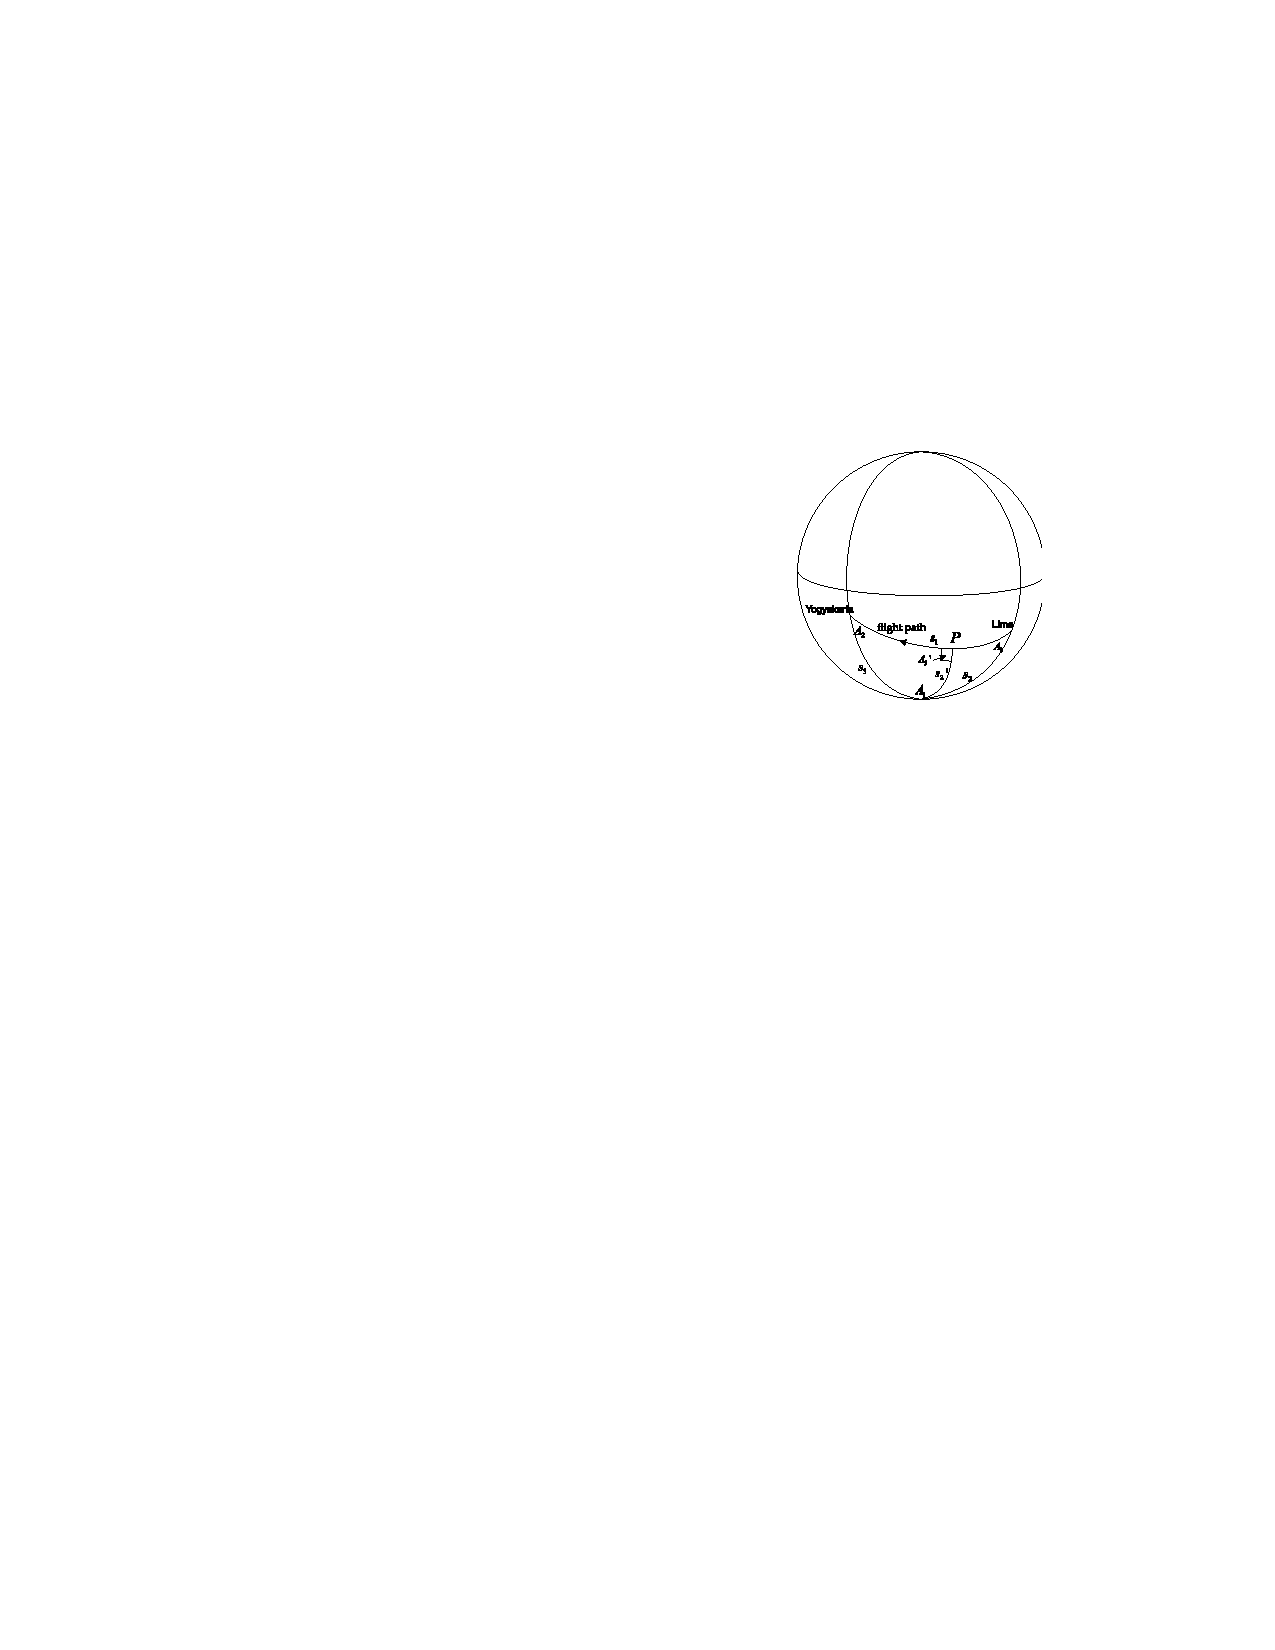
\includegraphics[pagebox=mediabox,viewport=376 455 504 576,clip,
      width=0.75\linewidth]{2015_TH_S15-s3.pdf}
  \end{center}
\end{description}

\solhead{1.21}{Shadows}
% source id: 2016_TH_T4
As the longest shadow of the Sun on the given day is of finite length, the
Sun is circumpolar for this observer on this day. \hfill[2.0]

\ioaafig{2016_TH_T4-s1.pdf}
In the figure, the left panel shows the shadow $OS$ formed by stick $OA$ (of
length 1.000\,m), and the right panel shows the Sun's location in two cases.

For an altitude $\theta$ of the Sun,
\[ \tan\theta = \frac{OA}{OS} = \frac{1.000\ \mathrm{m}}{OS} \]
\[ \therefore\ \cot\theta = OS\ \text{(in metres)} \]
\hfill[1.0]

Let $\theta_1$ and $\theta_2$ be the altitude in the two extreme cases.
\[ \theta_1 = 180^\circ - \phi - (90^\circ - \delta_\odot)
   = 90^\circ - \phi + \delta_\odot \]
\hfill[1.0]
\begin{align*}
\cot(90^\circ - \phi + \delta_\odot) &= 1.732\\
\therefore\ \tan(\phi - \delta_\odot) &= 1.732\\
\phi - \delta_\odot &= \tan^{-1}(1.732) = 60^\circ = 1.047\ \mathrm{rad}
\end{align*}
\hfill[1.5]
\[ \theta_2 = \phi - (90^\circ - \delta_\odot)
   = \phi - 90^\circ + \delta_\odot \]
\hfill[1.0]
\begin{align*}
\cot(\phi - 90^\circ + \delta_\odot) &= 5.671\\
\therefore\ \tan(\phi - 90^\circ + \delta_\odot) &= \frac{1}{5.671}\\
\phi + \delta_\odot &= \tan^{-1}\left(\frac{1}{5.671}\right) + 90^\circ
  = 100^\circ = 1.745\ \mathrm{rad}
\end{align*}
\hfill[1.5]

Solving,
\[ \boxed{\phi = 80^\circ} = 1.396\ \mathrm{rad} \]
\hfill[1.0]
\[ \boxed{\delta_\odot = 20^\circ} = 0.349\ \mathrm{rad} \]
\hfill[1.0]

Given high accuracy of shadow length, only $\pm 0.5^\circ$ is allowed.

One can also solve the question by manipulating $\tan(\phi - \delta_\odot)$
and $\tan(\phi + \delta_\odot)$, to get $\tan(\phi)$ and $\tan(\delta_\odot)$.

\solhead{1.22}{The Large Magellanic Cloud in Phuket}
% source id: 2017_TH_T1
\ioaafig{2017_TH_T1-s1.pdf}
When it culminates, $\mathrm{LHA} = 0$,
$\mathrm{RA} = -\mathrm{LST}$ \hfill[1.0]
\begin{align*}
\mathrm{LST} &= -(\mathrm{L} - \mathrm{GST}^{*}) = -\mathrm{RA}\\
\mathrm{GST}^{*} &= \mathrm{L} - \mathrm{RA}
  = 6^{\mathrm{h}}\,34^{\mathrm{min}} - 5^{\mathrm{h}}\,24^{\mathrm{min}}
  = 1^{\mathrm{h}}\,10^{\mathrm{min}}
\end{align*}
\hfill[2.0]
\begin{align*}
\mathrm{GST} &= 24^{\mathrm{h}} - 1^{\mathrm{h}}\,10^{\mathrm{min}}\\
\mathrm{GST} &= 22^{\mathrm{h}}\,50^{\mathrm{min}}
\end{align*}
\hfill[1.0]

Phuket time of 21:00 is UT\,14:00. \hfill[1.0]

\[ \mathrm{GST} = \text{GST of 1st Jan}
   + \text{The angle that $\Upsilon$ moves away from 1st Jan}
   + \mathrm{UT} \]
\hfill[1.0]
\begin{align*}
22^{\mathrm{h}}\,50^{\mathrm{min}}
  &= 6^{\mathrm{h}}\,43^{\mathrm{min}}
   + \left[\left(\frac{\text{Days that away from 1st Jan}}
                     {365.2422\ \text{days}}\right)\times 24\ \mathrm{h}\right]
   + \left[14^{\mathrm{h}}\times\left(\frac{24}{23.9344}\right)\right]\\
\text{Days that away from 1st Jan}
  &= (22^{\mathrm{h}}\,50^{\mathrm{min}} - 6^{\mathrm{h}}\,43^{\mathrm{min}}
    - 14^{\mathrm{h}}\,2^{\mathrm{min}})
    \left(\frac{365.2422\ \text{days}}{24^{\mathrm{h}}}\right)
\end{align*}
\hfill[2.0]

Days that away from 1st Jan $= 31.7$ days from 1st Jan (at Greenwich).
\hfill[1.0]

The time of the year that the LMC culminates in Phuket is on 2nd February.
\hfill[1.0]

\solhead{1.23}{Shipwreck}
% source id: 2017_TH_T12
\begin{description}
\item[a)] Draw a correct celestial sphere. \hfill[4.0]
  \ioaafig{2017_TH_T12-s1.pdf}
  \[ \frac{\sin\mathrm{LHA}^{*}}{\sin z}
     = \frac{\sin\mathrm{A}}{\sin(90^\circ - \delta)} \]
  \hfill[2.0]
  \begin{align*}
  \mathrm{LHA}^{*} &= \sin^{-1}\left(
    \frac{\sin\mathrm{A}\,\sin z}{\sin(90^\circ - \delta)}\right)\\
  &= \sin^{-1}\left(
    \frac{\sin 109^\circ\,\sin 37.5^\circ}{\sin 98.18^\circ}\right)
  \end{align*}
  \hfill[2.0]
  \[ \mathrm{LHA}^{*} = 35.56^\circ = 2^{\mathrm{h}}\,22\ \mathrm{min} \]
  \[ \mathrm{LHA} = 24^{\mathrm{h}} - 2^{\mathrm{h}}\,22\ \mathrm{min}
     = 21^{\mathrm{h}}\,38\ \mathrm{min} \]
  \hfill[2.0]

\item[b)] Bangkok time of 01:00 21st November is Universal Time (UT) 18:00
  20th November.

  Day number $+$ Time $= 323$ day 18\,h \hfill[1.0]

  GST $=$ GST of 1st Jan $+$ The angle that $\Upsilon$ moves away from 1st
  Jan \hfill[2.0]
  \[ \mathrm{GST} = 6^{\mathrm{h}}\,43^{\mathrm{min}}
     + \left(323\tfrac{18}{24}\ \mathrm{days}\right)
       \left(\frac{1}{365.2422}\right)\times 24\ \frac{\mathrm{h}}{\mathrm{day}}
     + \left[18\mathrm{h}\times\left(\frac{24}{23.9344}\right)\right] \]
  \hfill[5.0]
  \begin{align*}
  \mathrm{GST} &= 6^{\mathrm{h}}\,43^{\mathrm{min}}
    + 21^{\mathrm{h}}\,16\ \mathrm{min} + 18^{\mathrm{h}}\,3^{\mathrm{min}}\\
  \mathrm{GST} &= 46^{\mathrm{h}}\,2^{\mathrm{min}}\\
  \mathrm{GST} &= 21^{\mathrm{h}}\,58^{\mathrm{min}}
  \end{align*}
  \hfill[2.0]

  Any other correct alternative methods that provide the correct answer are
  also acceptable.

\item[c)]
  \ioaafig{2017_TH_T12-s2.pdf}
  \begin{align*}
  24^{\mathrm{h}} - \mathrm{LHA} &= \mathrm{RA} - \mathrm{LST}\\
  \mathrm{LST} &= \mathrm{RA} - 24^{\mathrm{h}} + \mathrm{LHA}\\
  \mathrm{L} &= \mathrm{RA} + \mathrm{LHA} - \mathrm{GST}\\
  \mathrm{L} &= 5^{\mathrm{h}}\,15^{\mathrm{min}}
    + 21^{\mathrm{h}}\,38\ \mathrm{min} - 21^{\mathrm{h}}\,58^{\mathrm{min}}
    = 4^{\mathrm{h}}\,55^{\mathrm{min}}
  \end{align*}
  \hfill[3.0]
  \[ \mathrm{L} = 73.75^\circ\,\mathrm{E} \]
  \hfill[2.0]

\item[d)]
  \begin{align*}
  \cos(90^\circ - \delta) &= \cos z\cos(90^\circ - \phi)
    + \sin z\sin(90^\circ - \phi)\cos\mathrm{A}\\
  \sin\delta &= \sin(h)\sin\phi + \cos(h)\cos\mathrm{A}\cos\phi
  \end{align*}
  \hfill[5.0]
  \[ \alpha = \sin\delta,\quad \beta = \sin(h),\quad
     \gamma = \cos(h)\cos\mathrm{A},\quad x = \sin\phi \]
  \[ \alpha = \beta x + \gamma\sqrt{1 - x^2} \]
  \[ (\beta^2 + \gamma^2)x^2 - 2\alpha\beta x + (\alpha^2 - \gamma^2) = 0 \]
  \hfill[1.0]
  \[ x = \frac{\alpha\beta \pm \gamma\sqrt{\gamma^2 + \beta^2 - \alpha^2}}
              {\beta^2 + \gamma^2} \]
  \hfill[1.0]
  \[ \sin\phi = \frac{\sin\delta\sin(h)
      \pm \cos(h)\cos\mathrm{A}
      \sqrt{(\cos(h)\cos\mathrm{A})^2 + \sin^2(h) - \sin^2\delta}}
     {\sin^2(h) + (\cos(h)\cos\mathrm{A})^2} \]
  \hfill[1.0]
  \[ \phi = -24.05^\circ,\ 4.01^\circ \]
  \hfill[2.0]

  For $\phi = -24.05^\circ\ \rightarrow\ \mathrm{A} = 71.0^\circ$
  \hfill[2.0]

  For $\phi = 4.01^\circ\ \rightarrow\ \mathrm{A} = 109^\circ$
  \hfill[2.0]

  The Latitude of the island is $4^\circ 1'$\,N. \hfill[1.0]
\end{description}

\textbf{Alternative Solutions}

\begin{description}
\item[b)] $-$LMT (Local Mean Time) $\rightarrow$ UT \hfill[1.0]

  Calculate the sidereal day using the given tropical year:
  \[ \gamma = \frac{\text{Sidereal time}}{\text{Solar time}}
     = \frac{24^{\mathrm{h}}\times\left(1
       + \dfrac{1}{T_{\mathrm{tropic}}}\right)}{24^{\mathrm{h}}}
     = 1 + \frac{1}{T_{\mathrm{tropic}}} = 1.002737909 \]
  \hfill[3.0]

  On the 21st November 2017, GST can be calculated from GST on 1st January
  2017.

  Day number $+$ Time $= 323$\,d 18\,h \hfill[2.0]
  \[ \mathrm{GST} = \mathrm{GST}_0 + \Delta\theta
     = \mathrm{GST}_0 + \gamma\cdot\Delta\mathrm{T} \]
  \hfill[2.0]
  \begin{align*}
  \Delta\theta &= \left(323^{\mathrm{d}}\ \tfrac{18}{24}\right)
    \cdot 1.002737909\\
  &= 324^{\mathrm{d}}.6363981
   = 15^{\mathrm{h}}16^{\mathrm{m}}24^{\mathrm{s}}.8\\
  \mathrm{GST} &= \mathrm{GST}_0
    + 15^{\mathrm{h}}16^{\mathrm{m}}24^{\mathrm{s}}.8\\
  &= 6^{\mathrm{h}}43^{\mathrm{m}}
   + 15^{\mathrm{h}}16^{\mathrm{m}}24^{\mathrm{s}}.8\\
  &= 21^{\mathrm{h}}59^{\mathrm{m}}24^{\mathrm{s}}.8
  \end{align*}
  \hfill[2.0]

\item[d)] From Cosine law:
  \begin{align*}
  \sin\delta &= (\cos z)\cdot\sin\phi + (\sin z\cos A)\cdot\cos\phi\\
  \cos z &= (\sin\delta)\cdot\sin\phi
    + (\cos\delta\cos\mathrm{LHA}^{*})\cdot\cos\phi
  \end{align*}
  \hfill[5.0]

  Correct calculation steps that can lead to the final answers. \hfill[5.0]

  Final answers:
  \[ \sin\phi = 0.0698,\quad \phi = 4.00^\circ \]
  OR
  \[ \cos\phi = 0.9976,\quad \phi = 4.00^\circ \]
  \hfill[5.0]
\end{description}

\solhead{1.24}{A Synchronous Satellite}
% source id: 2017_TH_T5
\ioaafig[1.0]{2017_TH_T5-s1.pdf}
Draw diagram and correctly identify the altitude. \hfill[1.0]

Identify another angle with the altitude $h$ in its expression, such as
$90^\circ - (\phi - \theta) - h$. \hfill[1.0]

Maximum altitude occurs when the satellite is at meridian. \hfill[1.0]

Intermediate steps that can lead to the calculation of $h$, such as
\[ \tan(90^\circ - (\phi - \theta) - h)
   = \frac{R\sin(\phi - \theta)}{H + R - R\cos(\phi - \theta)} \]
\hfill[3.0]

Correct expression for $h$: \hfill[2.0]
\[ h = 90^\circ - (\phi - \theta)
   - \tan^{-1}\left(\frac{R\sin(\phi - \theta)}
                        {H + R - R\cos(\phi - \theta)}\right) \]

Correct value of $h$:
\[ h = 90^\circ - (51.49^\circ - 6.69^\circ)
   - \tan^{-1}\left(\frac{\sin(51.49^\circ - 6.69^\circ)}
     {\dfrac{35.786\ \mathrm{km}}{6.38\times 10^{3}\ \mathrm{km}}
      + 1 - \cos(51.49^\circ - 6.69^\circ)}\right) \]
\[ h = 38.4^\circ \]
\hfill[2.0]

\emph{Maximum of 2.0 marks for solution with}
$h = 90.0^\circ - 51.49^\circ + 6.69^\circ = 45.2^\circ$.

\solhead{1.25}{Vega and Altair}
% source id: 2018_TH_T10
\begin{description}
\item[(a)] Assuming the positions of the two stars are: Vega:
  $(\alpha_1, \delta_1)$; Altair: $(\alpha_2, \delta_2)$
  \[ (\alpha_1, \delta_1) = (279.23538^\circ,\ 38.78547^\circ)
     \quad\text{and}\quad
     (\alpha_2, \delta_2) = (297.69875^\circ,\ 8.87036^\circ) \]
  \hfill(2 points)

  Cosine formula of the spherical geometry is given by:
  \[ \cos[a] = \cos[b]\cos[c] + \sin[b]\sin[c]\cos[A] \]
  \hfill(0.5 point)

  In our triangle, $b = (90 - \delta_1)$, $c = (90 - \delta_2)$ and
  $A = (\alpha_2 - \alpha_1)$. Then the angular distance $\beta$ between
  Vega and Altair is:
  \[ \cos[\beta] = \cos[90^\circ - \delta_1]\cos[90^\circ - \delta_2]
     + \sin[90^\circ - \delta_1]\sin[90^\circ - \delta_2]
       \cos[\alpha_2 - \alpha_1]; \]
  \hfill(3 points)
  \[ \cos[\beta] = \cos[51.21453^\circ]\cos[81.12964^\circ]
     + \sin[51.21453^\circ]\sin[81.12964^\circ]\cos[18.46337^\circ]; \]
  \hfill(1.5 points)
  \[ \beta = 34.19582^\circ \]
  \hfill(2 points)

\item[(b)] The distance of Vega is:
  $r_1 = 1/(130.23\times 10^{-3}) = 7.6787\,pc$

  The distance of Altair is:
  $r_2 = 1/(194.95\times 10^{-3}) = 5.1295\,pc$ \hfill(2 points)

  Using the Law of Cosines:
  $d^2 = r_1^{\,2} + r_2^{\,2} - 2r_1 r_2\cos[\beta]$ \hfill(2 point)

  we can obtain the distance: $d = 4.4855\,pc$ \hfill(2 points)

\item[(c)] Given the proper motions and radial velocities of the two stars,
  the directions of their movements on the celestial sphere can be
  estimated.

  For Vega:
  \begin{align*}
  \mu_{\alpha 1}\cos\delta_1 &= 200.94;\ \mu_{\delta 1} = 286.23\\
  \theta_1 &= \arctan\left[\frac{\mu_{\alpha 1}\cos\delta_1}
    {\mu_{\delta 1}}\right]\times\frac{180^\circ}{\pi} = 35.0697^\circ
  \end{align*}
  \hfill(2 points)

  For Altair:
  \begin{align*}
  \mu_{\alpha 2}\cos\delta_2 &= 536.23;\ \mu_{\delta 2} = 385.29\\
  \theta_2 &= \arctan\left[\frac{\mu_{\alpha 2}\cos\delta_2}
    {\mu_{\delta 2}}\right]\times\frac{180^\circ}{\pi} = 54.302^\circ
  \end{align*}
  \hfill(1 points)

\item[(d)] As the position angles of the proper motion of the two stars are
  different, the stars' paths will intersect. As the paths are circular on
  the celestial sphere, they will intersect in exactly \textbf{two} points.
  \hfill(2 points)

\item[(e)] Let the closer point of intersection be I with the coordinates
  $(\alpha_3, \delta_3)$.

  In triangle PVA,
  \[ PAV = \arcsin\left[\frac{\sin VPA\,\sin PV}{\sin VA}\right]
     = \arcsin\left[\frac{\sin(\alpha_1 - \alpha_2)
       \sin(90^\circ - \delta_1)}{\sin\beta}\right] = 26.055^\circ \]
  \[ PVA = \arcsin\left[\frac{\sin VPA\,\sin PA}{\sin VA}\right]
     = \arcsin\left[\frac{\sin(\alpha_1 - \alpha_2)
       \sin(90^\circ - \delta_2)}{\sin\beta}\right] = 146.196^\circ \]
  \hfill(5 points)

  Note that angle PVA is more than $90^\circ$, which will be evident from
  the diagram. \hfill(1 point)

  The motion of the stars on the celestial sphere will always be along some
  great circle. So VAI is a spherical triangle. Using the four parts formula
  for VAI
  \[ \cot VI = \frac{\cos VA\cos IVA + \sin IVA\cot VAI}{\sin VA} \]
  \[ VI = 90^\circ - \arctan\left[\frac{\cos 34.19582^\circ
     \cos(68.900^\circ) + \sin(68.900^\circ)\cot(99.643^\circ)}
     {\sin 34.19582^\circ}\right] = 76.085^\circ \]
  \hfill(5 points)

  by sine rule,
  \[ AI = \arcsin\left[\frac{\sin VI\sin IVA}{\sin VAI}\right]
     = \arcsin\left[\frac{\sin 76.085^\circ\sin 68.900^\circ}
       {\sin 99.643^\circ}\right] = 66.715^\circ \]
  \hfill(2 points counted in next part)

  Now we use triangle PVI: by cosine rule,
  \begin{align*}
  \cos[PI] &= \cos[PV]\cos[VI] + \sin[PV]\sin[VI]\cos[PVI];\\
  \cos[90^\circ - \delta_3] &= \cos[90^\circ - \delta_1]\cos[VI]
    + \sin[90^\circ - \delta_1]\sin[VI]\cos[180^\circ - \theta_1];\\
  \sin[\delta_3] &= \cos[51.215^\circ]\cos[76.085^\circ]
    + \sin[51.215^\circ]\sin[76.085^\circ]\cos[144.930^\circ];
  \end{align*}
  Thus, $\delta_3 = -27.945^\circ$ \hfill(4 points)

  Applying sine rule,
  \[ VPI = \arcsin\left[\frac{\sin PVI\sin VI}{\sin PI}\right]
     = \arcsin\left[\frac{\sin 144.930^\circ\sin 76.085^\circ}
       {\sin 117.945^\circ}\right] = 39.148^\circ \]
  Hence,
  $\alpha_3 = \alpha_1 - VPI = 279.235^\circ - 39.148^\circ = 240.087^\circ
   \approx 16^{\mathrm{h}}0^{\mathrm{m}}21^{\mathrm{s}}$ \hfill(5 points)

  Out of 5 points, 1 point is reserved for realising that the intersection
  point is in the past path.

\item[(f)] The total velocity along the great circle for Vega is
  \[ \mu_1 = \sqrt{(\mu_{\alpha 1}\cos\delta_1)^2 + \mu_{\delta 1}^{\,2}}
     = \sqrt{200.94^2 + 286.23^2} = 349.72\ \text{mas/year} \]
  \hfill(2 points)
  \[ \text{Number of years} = \frac{VI}{\mu_1}
     = \frac{76.085\times 3600}{0.34972} \approx 783200\ \text{years} \]
  It will happen in the year 781200 BCE. \hfill(2 points)

  Similarly, $\mu_2 = 660.30$ and number of years $= 363700$ years.

  It will happen in the year 3617 BCE.
  % sic: source says "3617 BCE"; 363700 years ago would be ~361700 BCE
  \hfill(2 points)

\item[(g)] After 363700 years, Vega would have traversed $35.335^\circ$
  along its path. \hfill(3 points)

  Thus, its separation from Altair will be
  $(76.085^\circ - 35.335^\circ) = 40.750^\circ$ \hfill(2 points)

\item[(h)] In earth centric Cartesian frame, coordinates of Vega (in units
  of parsec) will be:
  \begin{align*}
  x_1 &= r_1\cos\delta_1\cos(360^\circ - \alpha_1) = 0.96062\,\text{pc}\\
  y_1 &= r_1\cos\delta_1\sin(360^\circ - \alpha_1) = 5.90793\,\text{pc}\\
  z_1 &= r_1\sin\delta_1 = 4.80998\,\text{pc}
  \end{align*}
  Similarly, coordinates of Altair will be, $x_2 = 2.35579$,
  $y_2 = 4.48736$\,pc and $z_2 = 0.79097$\,pc. \hfill(6 points)

  Here, we are assuming the North as positive x-direction and pole as
  positive z-direction.

  The direction vectors for velocities in spherical coordinates are
  \[ v_1 = (-13.9, 7.33, 10.45)\quad\text{and}\quad
     v_2 = (-26.9, 19.57, 14.06) \]
  % sic: source uses radial velocity -26.9 for Altair though the problem
  % table gives -26.1; Altair's tangential components also appear to be
  % computed with Vega's distance (7.6787 pc) rather than Altair's
  \hfill(4 points)

  The same in Cartesian coordinates will be
  \begin{align*}
  v_{x1} &= v_{r1}\cos\delta_1\cos\alpha_1 - v_{\alpha 1}\sin\alpha_1
    - v_{\delta 1}\sin\delta_1\cos\alpha_1 = 4.45\\
  v_{y1} &= -v_{r1}\cos\delta_1\sin\alpha_1 - v_{\alpha 1}\cos\alpha_1
    + v_{\delta 1}\sin\delta_1\sin\alpha_1 = -18.33\\
  v_{z1} &= v_{r1}\sin\delta_1 + v_{\delta 1}\cos\delta_1 = -0.56
  \end{align*}
  Similarly, Cartesian velocity vector of Altair will be,
  $v_2 = (4.33, -33.85, 9.87)$. \hfill(8 points)

  Lastly, we evaluate the value of the determinant,
  \[ \begin{vmatrix}
     (x_1 - x_2) & (y_1 - y_2) & (z_1 - z_2)\\
     v_{x1} & v_{y1} & v_{z1}\\
     v_{x1} & v_{y1} & v_{z1}
     % sic: source labels the third row with Vega's components again;
     % the numbers below are Altair's
     \end{vmatrix}
   = \begin{vmatrix}
     -1.40 & 1.42 & 4.02\\
     4.45 & -18.33 & -0.56\\
     4.33 & -33.85 & 9.87
     \end{vmatrix} \]
  \[ = 279.82 - 65.81 - 286.48 = -72.47 \]
  As the value of the determinant is non-zero, the direction vectors of
  these two stars do not cross each other. Hence no such point can exist.
  \hfill(4 points)
\end{description}

\solhead{1.26}{Distance}
% source id: 2018_TH_T2
T F T F T \hfill(2 points each)

For parallaxes, we have a Gaussian with $\mu = 0.2$\,mas and
$\sigma = 0.05$\,mas, i.e.\ 25\% of the expectation value.

If we assume that the lowest and highest values of parallax are symmetric
w.r.t.\ the expected value (reasonable assumption if cluster has large
number of stars), then their distances would not be symmetric w.r.t.\ the
true distance.

$R_A > R$, $R_C = R$ (for statements (m) and (o), marks will be given only
if this relation is stated).

\solhead{1.27}{Atmospheric Refraction}
% source id: 2018_TH_T3
\begin{description}
\item[(a)] $r_d < r_u < r_l = r_r$ \hfill(4 points)
\item[(b)] When the upper edge of the Sun is under the horizon by $35'$, it
  will appear on the horizon earlier due to the influence of atmospheric
  refraction. With the apparent diurnal motion, i.e.
  \[ \omega = \frac{360^\circ}{23^{\mathrm{h}}56^{\mathrm{m}}4^{\mathrm{s}}}
     = \frac{21600'}{1436.0682^{\mathrm{m}}} = 15.0411\,'/m, \]
  \hfill(2 points)

  Ideally one should find the time taken by the mean sun to travel from
  $50'$ below horizon to $15'$ below true horizon.
  \[ \Delta t = \frac{(50' - 15')}{\omega\cos\varphi}
     = \frac{35'}{15.0411'\times\cos 40^\circ} = 3.04\ \mathrm{mins} \]
  \hfill(4 points)
\end{description}

\solhead{1.28}{Height of a Hill}
% source id: 2018_TH_T4
\ioaafig[1.0]{2018_TH_T4-s1.pdf}
First we should realise that the Sun doesn't set vertically. It sets at an
angle of $\theta = 90 - \varphi = 50^\circ$. Thus, the horizon depression
$x$ will be
\[ x = 15.0411' \times 4.1 \times \sin\theta
   = 1.03^\circ \sin 50^\circ = 0.787^\circ. \]
\hfill(4 points)

Let the height of the mountain be $H$. Let $C$ be the centre of the Earth,
point $T$ the hill top and point $T'$ the point on the horizon as seen from
$T$. Thus,
\[ \cos x = \left[\frac{R_\oplus}{(R_\oplus + H)}\right] \]
\[ H = \frac{R_\oplus(1 - \cos x)}{\cos x} = 602\ \mathrm{metres} \]
\hfill(3 points)

The distance of the horizon (from the base of the mountain, along the
surface of the earth) is found from the rectangular triangle $TCT'$ as
\[ D = (R_\oplus + H)\sin x \approx R_\oplus\sin x
   = 6.38\times 10^{3}\,\sin 0.787^\circ = 87.6\ \mathrm{km} \]
Alternatively,
\[ D = R_\oplus x = 6.38\times 10^{3}\times 0.787^\circ\times\pi
   \div 180^\circ = 87.6\ \mathrm{km} \]
\hfill(3 points)

\solhead{1.29}{Sidereal Time}
% source id: 2018_TH_T5
\begin{description}
\item[(1)] This can happen if the sidereal time is 00:00:00 just after the
  midnight and just before the midnight on the same day. It means that the Sun
  should be near the Autumn (September) Equinox. Approximate R.A. of the Sun is
  $18^{\mathrm{h}}$.
  % sic: the official solution says 18 h; at the September equinox the Sun's
  % R.A. is 12 h.
  \hfill(3 points)
\item[(2)] At $0^{\mathrm{h}}$, 1st January, 2018 (JD\,2458119.5), the mean
  sidereal time $\mathrm{GMST}_0$ was $6.706^{\mathrm{h}}$, i.e.
  $\mathrm{GMST}_0 = 100.59^\circ$. Since one mean solar day is longer than one
  mean sidereal day by $0.9856^\circ$ (about 4 minutes), the GMST will increase
  by $\Delta = 0.9856^\circ$ at next midnight on 2nd January, 2018. Therefore,
  we can first calculate how many days it will take for GMST to reach
  $360^\circ$, i.e.
  \[
    T = \frac{360^\circ - \mathrm{GMST}_0}{\Delta}
      = \frac{360^\circ - 100.59^\circ}{0.9856^\circ} = 263.20
  \]
  \hfill(3 points)

  i.e.\ after completion of 263 days, the GMST at midnight will be
  $359.80^\circ$.

  Thus, GMST will be 00:00:00 on the 264th day at 00:00:48 and then again at
  23:56:52 on the same day. \hfill(2 points)

  The 264th day in the calendar of 2018 is 21st September 2018.
  \hfill(2 points)
\end{description}

\solhead{1.30}{South to East to North}
% source id: 2019_TH_10
\begin{description}
\item[1.] The trivial solution of the problem is the North Pole ($N$). Starting
  from here we travel 6378\,km to the South ($\overset{\frown}{NA}$) along a meridian
  (e.g.\ Greenwich meridian), then 6378\,km to the East along a parallel
  ($\overset{\frown}{AB}$), and finally 6378\,km to the North ($\overset{\frown}{BN}$) (see
  figure~(a), where the black dashed lines are the Equator and the Greenwich
  meridian).

  For the general solution, mark the path to be taken in one direction with $s$
  and determine what it may be!

  Let us denote the longitude and latitude of the point $A$ by $\lambda_A$ and
  $\varphi_A$, and the point $B$ by $\lambda_B$ and $\varphi_B$.

  The triangle $ANB$ is a spherical one only if the points $A$ and $B$ are on
  the Equator (see figure~(b)), i.e.\ $\varphi_A = \varphi_B = 0^\circ$ and
  $s = R\pi/2$, because the arc $\overset{\frown}{AB}$ is lying along a great circle
  only in this case, otherwise it is a part of a parallel. The point $A$ and
  $B$ can be below the Equator as well (figure~(c)).

  \ioaafig[1.0]{2019_TH_10-s1.pdf}

  Next, we measure the angles in radians.

  The central angle of the arc $\overset{\frown}{NA}$ on the meridian fitting to the
  point $A$ ($O$ is the centre of the sphere):
  \[
    NOA\sphericalangle = \frac{\pi}{2} - \varphi,
    \quad\text{where } \varphi = \varphi_A = \varphi_B \tag{10.1}
  \]
  Thus the length $s$ of the arc $\overset{\frown}{NA}$:
  \[
    s = R\left(\frac{\pi}{2} - \varphi\right),
    \quad\text{where } s < R\pi \tag{10.2}
  \]
  The radius of the latitude circle fitting to the points $A$ and $B$:
  \[
    r_{AB} = R\sin\left(\frac{\pi}{2} - \varphi\right) = R\cos\varphi
    \tag{10.3}
  \]
  The central angle of the arc $\overset{\frown}{AB}$ is $\lambda_B - \lambda_A$,
  thus the length of the arc $\overset{\frown}{AB}$:
  \[
    s = r_{AB}\,(\lambda_B - \lambda_A) = R\cos\varphi\,(\lambda_B - \lambda_A)
    \tag{10.4}
  \]
  From the Eq.~(10.2) and Eq.~(10.4):
  \[
    \varphi = \frac{\pi}{2} - \frac{s}{R}
    \quad\text{and}\quad
    \lambda_B - \lambda_A = \frac{s}{R\cos\varphi} \tag{10.5}
  \]
  Substitute the expression of $\varphi$ from the first equation into the
  second equation:
  \[
    \lambda_B - \lambda_A = \frac{s}{R\cos\varphi}
      = \frac{\dfrac{s}{R}}{\cos\left(\dfrac{\pi}{2} - \dfrac{s}{R}\right)}
      = \frac{\dfrac{s}{R}}{\sin\dfrac{s}{R}} \tag{10.6}
  \]
  For a given arc length of $s$ ($s < R\pi$) the latitude $\varphi$ of the
  points $A$ and $B$, and the difference between their longitudes we can
  calculate from the following equations:
  \[
    \varphi = \frac{\pi}{2} - \frac{s}{R}
    \quad\text{and}\quad
    \lambda_B - \lambda_A = \frac{\dfrac{s}{R}}{\sin\dfrac{s}{R}} \tag{10.7}
  \]

  ***** Supplement. It is just for the sake of completeness, not necessary for
  the full marks.

  It is well known, that
  \[
    \lim_{x\to 0}\frac{\sin x}{x} = \lim_{x\to 0}\frac{x}{\sin x} = 1,
    \tag{10.8}
  \]
  thus $\lambda_B - \lambda_A = 1$ in case of $s \to 0$.

  Therefore the difference in longitude has a lower limit (1), but it has no
  upper limit. This means, that the distance between the points $A$ and $B$
  will increase by increasing $s$, the difference between their longitudes will
  approximate $2\pi$ (see figure~(d)), and in case of
  $\lambda_B - \lambda_A = 2\pi$ the points $A$ and $B$ will be the same (see
  figure~(e)). With further increasing of $s$ the difference
  $\lambda_B - \lambda_A$ will be larger than $2\pi$ (see figure~(f)), thus we
  have to stop at that point on the circle where the length of the path along
  it reaches the value of $s$, and then turn to the North.

  \ioaafig{2019_TH_10-s2.pdf}

  The arc length $s_{\lim}$ corresponding to the ``limit case'' of
  $\lambda_B - \lambda_A = 2\pi$ we can derive from the numerical solution of
  the following transcendent equation:
  \[
    \frac{s_{\lim}}{R} - 2\pi\sin\frac{s_{\lim}}{R} = 0
  \]
  Thus find the root of the function
  \[
    f(s) = \frac{s}{R} - 2\pi\sin\frac{s}{R},
  \]
  i.e.\ the value $s_{\lim}$, where $f(s_{\lim}) = 0$. We can solve it by
  iteration using e.g.\ the Newton--Raphson method:
  \[
    s_{k+1} = s_k - \frac{f(s_k)}{f'(s_k)}, \qquad k = 0, 1, 2, \ldots
  \]
  The first derivative of the function $f(s)$:
  \[
    f'(s) = \frac{1}{R} - \frac{2\pi}{R}\cos\frac{s}{R}
  \]
  We know that the parallel in question runs south from the Equator, thus a
  good initial value for the iteration could be $s_0 = R\pi/2 + \Delta s$,
  where $\Delta s = 1000$\,km.

  The result of the iteration and the corresponding latitude with three decimal
  places:
  \[
    s_{\lim} = 17\,206.566\ \mathrm{km}, \quad
    \varphi_{\lim} = -64.573^\circ
  \]
  $\lambda_B - \lambda_A$ is strictly increasing function of $s$ and
  \[
    \lim_{s/R\to 0} \lambda_B - \lambda_A = 1, \quad
    \lim_{s/R\to \pi} \lambda_B - \lambda_A = \infty, \tag{10.9}
  \]
  thus for any values of $0 < s < R\pi$ can be found an appropriate angle
  $\lambda_B - \lambda_A$.

  \ioaafig{2019_TH_10-s3.pdf}

  ***** End of supplement.

  In conclusion, the solution in this case is the North Pole ($N$).
  \hfill(2\,p)

  For the value of $s = 6378$\,km the solution is an (a)-type curve. The
  coordinates of the turning points are:
  \[
    \lambda_A = 0^\circ, \quad \lambda_B = 68.09^\circ, \quad
    \varphi_A = \varphi_B = 32.704^\circ
  \]
  \hfill(3\,p)

\item[2.] The non-trivial solutions are similar to the (e)-type (``lasso'')
  solution of the previous part, only the starting point is not the North Pole,
  but its location depends on the given value of arc length $s$. The circle of
  the lasso will run south from the (e)-type ``limit circle'', because the
  circumference of parallels running north from it are greater than the
  north--south arc.

  The procedure is the following.

  Knowing $s$, we have to find the parallel around the South Pole ($S$), whose
  circumference is an integer multiple of $s$. \hfill(2\,p)

  If the corresponding latitude is $\varphi_D$, then:
  \[
    2k\pi R\cos\varphi_D = s, \quad k = 1, 2, 3, \ldots \tag{10.10}
  \]
  \hfill(5\,p)

  If the latitude of the sought starting point $C$ is $\varphi_C$, then the
  length $s$ of the arc to be taken along the meridian:
  \[
    s = R\,(\varphi_C - \varphi_D) \tag{10.11}
  \]
  From the Eqs.~(10.10) and (10.11):
  \[
    \varphi_C = \varphi_D + 2k\pi\cos\varphi_D, \quad k = 1, 2, 3, \ldots
    \tag{10.12}
  \]
  Thus:
  \[
    \varphi_D = -\arccos\frac{s}{2k\pi R}, \quad k = 1, 2, 3, \ldots
    \tag{10.13}
  \]
  \hfill(2\,p)

  and
  \[
    \varphi_C = -\arccos\frac{s}{2k\pi R} + \frac{s}{R},
    \quad k = 1, 2, 3, \ldots \tag{10.14}
  \]
  \hfill(2\,p)

  The negative sign denotes that the parallel is in the southern hemisphere.

  So if the starting point is not the North Pole ($N$), there are infinitely
  many solutions.

  For the value of $s = 6378$\,km the first 5 ($k = 1, \ldots, 5$) value for
  $\varphi_D$ in degrees with 3 decimal places:
  \[
    \varphi_{D_1} = -80.842^\circ,\ \varphi_{D_2} = -85.436^\circ,\
    \varphi_{D_3} = -86.959^\circ,\ \varphi_{D_4} = -87.72^\circ,\
    \varphi_{D_5} = -88.176^\circ
  \]
  \hfill(2\,p)

  The first 5 ($k = 1, \ldots, 5$) value for $\varphi_C$ in degrees with 3
  decimal places:
  \[
    \varphi_{C_1} = -23.546^\circ,\ \varphi_{C_2} = -28.14^\circ,\
    \varphi_{C_3} = -29.663^\circ,\ \varphi_{C_4} = -30.424^\circ,\
    \varphi_{C_5} = -30.88^\circ
  \]
  \hfill(2\,p)

  In conclusion, starting to the South from a point of the parallel marked with
  a dashed red line ($C$), we get to a point on a parallel marked with a
  continuous red line ($D$). On this parallel we travel a full circle to the
  East, then we get back to the point $D$, then turn to North and travel back
  to starting point $C$.

  For the further values of $k$ the procedure is very similar, but we have to
  perform two full circles along the continuous green parallel, three along the
  blue, four along the gold, five along the brown and so on.

  Such kind of solution exists for any values of $0 < s < s_{\lim}$.

  \ioaafig{2019_TH_10-s4.pdf}
\end{description}

\solhead{1.31}{Distance to a Near-Earth Asteroid}
% source id: 2019_TH_12
\begin{description}
\item[a)] The geometric situation is the following: \hfill(5\,p)

  \ioaafig{2019_TH_12-s1.pdf}

\item[b)] One can recognize that the triangle $NOW$ is an isosceles triangle,
  two sides ($ON$ and $OW$) are equal to each other in length:
  \[
    ON = OW = R \tag{12.1}
  \]
  \hfill(1\,p)

  Therefore the angles $\alpha = ONW\sphericalangle = OWN\sphericalangle$. For
  the $NOW$ triangle we can write, that:
  \[
    2\alpha + \varphi_1 + \varphi_2 = 180^\circ
    \;\rightarrow\;
    \alpha = 90^\circ - \frac{\varphi_1 + \varphi_2}{2} \tag{12.2}
  \]
  \hfill(1\,p)

  Let us denote the direct -- i.e.\ measured through the body of the Earth, not
  on the surface -- distance between Nagykanizsa and Windhoek by $d$:
  $d = NW$. This distance can be obtained straightforward by the cosine theorem
  (one has to take care that the absolute values of the latitudes should be
  added inside the cosine function):
  \[
    d = \sqrt{R^2 + R^2 - 2R^2\cos(\varphi_1 + \varphi_2)}
      = R\sqrt{2\bigl(1 - \cos(\varphi_1 + \varphi_2)\bigr)} \tag{12.3}
  \]
  \hfill(2\,p)

  With numerical values:
  \[
    d = 1.133\,05\,R
  \]
  \hfill(1\,p)

  Let us use the following notations:
  \[
    x_1 = \overline{NA}, \quad x_2 = \overline{WA}, \quad p = p_1 + p_2
    \tag{12.4}
  \]
  For the $NOWA$ quadrilateral we can write that:
  \[
    \varphi_1 + \varphi_2 + (180^\circ - z_1) + p + (180^\circ - z_2)
      = 360^\circ \tag{12.5}
  \]
  \hfill(1\,p)

  and therefore:
  \[
    p = z_1 + z_2 - (\varphi_1 + \varphi_2) \tag{12.6}
  \]
  \hfill(1\,p)

  For the $NWA$ triangle we can write that:
  \[
    \frac{x_1}{d} = \frac{\sin(180^\circ - z_2 - \alpha)}{\sin p}
    \quad\text{and}\quad
    \frac{x_2}{d} = \frac{\sin(180^\circ - z_1 - \alpha)}{\sin p} \tag{12.7}
  \]
  \hfill(2\,p)

  Thus:
  \[
    x_1 = d\,\frac{\sin(z_2 + \alpha)}
                  {\sin(z_1 + z_2 - (\varphi_1 + \varphi_2))}
    \quad\text{and}\quad
    x_2 = d\,\frac{\sin(z_1 + \alpha)}
                  {\sin(z_1 + z_2 - (\varphi_1 + \varphi_2))} \tag{12.8}
  \]
  \hfill(2\,p)

  $D$ can be obtained either from the triangle $NOA$ or $WOA$ by the cosine
  theorem:
  \[
    D^2 = R^2 + x_1^2 - 2Rx_1\cos(180^\circ - z_1) \tag{12.9}
  \]
  or
  \[
    D^2 = R^2 + x_2^2 - 2Rx_2\cos(180^\circ - z_2) \tag{12.10}
  \]
  \hfill(2\,p)

  Let us take the sum of them:
  \[
    2D^2 = 2R^2 + (x_1^2 + x_2^2) + 2R(x_1\cos z_1 + x_2\cos z_2),
    \tag{12.11}
  \]
  \hfill(1\,p)

  where we have used that $\cos(180^\circ - x) = -\cos x$.

  (If someone determines $D$ only from one of the two ($NOA$, $WOA$)
  triangles, 1 point can be deducted, because that means, we ignore the error
  bars of one of the measurements in a significant way.)

  After substitution and dividing by two one gets:
  \[
    D^2 = R^2
      + d^2\,\frac{\sin^2(z_1 + \alpha) + \sin^2(z_2 + \alpha)}
                  {2\sin^2(z_1 + z_2 - (\varphi_1 + \varphi_2))}
      + Rd\,\frac{\sin(z_2 + \alpha)\cos z_1 + \sin(z_1 + \alpha)\cos z_2}
                 {\sin(z_1 + z_2 - (\varphi_1 + \varphi_2))} \tag{12.12}
  \]
  \hfill(3\,p)

  This contains only known quantities. After substitution we get (notice that
  for alpha and $D$ we need the absolute values of the geographical latitudes):
  \[
    \alpha = 55.5^\circ
  \]
  \hfill(1\,p)
  \[
    D = 65.8\,R = 1.1\,d_{\mathrm{Moon}}
  \]
  \hfill(2\,p)

  So, the asteroid is at 65.8 Earth-radii from the centre of the Earth. This is
  slightly more than the distance to the Moon.
\end{description}

\solhead{1.32}{The height of the chimney of Tiszaujvaros power plant}
% source id: 2019_TH_6
\begin{description}
\item[a)] (B) the one on December 16 \hfill(1\,p)

  At a given moment of the day, the Sun elevation is lower in winter on the
  northern hemisphere.

\item[b)] (B) late in the morning \hfill(1\,p)

  The shadows point slightly west of north. In fact these satellite images are
  taken at around 9:45 UTC (10:45 Central European Time).

\item[c)] The measured shadow lengths are $x_1 = 125$\,m (epoch 1, summer
  solstice) and $x_2 = 780$\,m (epoch 2, winter solstice).

  Let the unknown height of the chimney be $h$. The chimney and its shadow form
  the legs of a right-angled triangle and thus
  \begin{align*}
    \tan\alpha_1 &= h/x_1 \tag{6.1}\\
    \tan\alpha_2 &= h/x_2, \tag{6.2}
  \end{align*}
  \hfill(1\,p)

  where $\alpha_1$ and $\alpha_2$ are the Sun elevation angles at epoch 1 and
  epoch 2, respectively. \hfill(1\,p)

  At the time of the summer and winter solstices, the Earth is located at
  opposite sides of the Sun during its orbital revolution. Since the Equator is
  tilted by $\varepsilon \approx 23.5^\circ$ to the orbital plane, at a given
  point of the surface, and at a given time of the day, the Sun elevation
  angles will differ by $\alpha_1 - \alpha_2 = 2\varepsilon$ (here we ignore
  refraction and that the satellite images were not taken on the exact solstice
  days). \hfill(4\,p)

  Notice that, to a good approximation, $\alpha_1 - \alpha_2 \approx 45^\circ$.
  Assuming $\alpha_1 = \alpha_2 + 45^\circ$ makes the solution a lot easier.
  Using the trigonometric identity
  \[
    \tan\alpha_1 = \tan(\alpha_2 + 45^\circ)
      = \frac{\tan\alpha_2 + \tan 45^\circ}{1 - \tan\alpha_2 \tan 45^\circ},
    \tag{6.3}
  \]
  and substituting $\tan 45^\circ = 1$, Eq.~(6.3) becomes
  \[
    \tan\alpha_1 = \frac{1 + \tan\alpha_2}{1 - \tan\alpha_2}. \tag{6.4}
  \]
  \hfill(4\,p)

  Substituting $\tan\alpha_1$ and $\tan\alpha_2$ from Eqs.~(6.1) and (6.2) into
  Eq.~(6.4), one gets a quadratic equation for the unknown $h$:
  \[
    \frac{h}{x_1} = \frac{1 + \dfrac{h}{x_2}}{1 - \dfrac{h}{x_2}}. \tag{6.5}
  \]
  \hfill(2\,p)

  Reducing this equation to the standard format
  \[
    h^2 + h(x_1 - x_2) + x_1 x_2 = 0, \tag{6.6}
  \]
  and according to the quadratic formula, the two roots are obtained as
  \[
    h_{1,2} = \frac{x_2 - x_1 \pm \sqrt{(x_1 - x_2)^2 - 4x_1x_2}}{2}. \tag{6.7}
  \]
  \hfill(1\,p)

  Now with the measured values of $x_1 = 125$\,m and $x_2 = 780$\,m, the two
  roots for $h$ are $h_1 = 426$\,m and $h_2 = 229$\,m. \hfill(1\,p)

  Obviously, only one of the solutions is valid for our case.

  One may simply notice that $h_1 \approx 426$\,m seems just too high for a
  chimney (would in fact be comparable to the Empire State Building in New
  York, with 443\,m; the Eiffel tower in Paris is only 324\,m high).

  Alternatively, substituting $h_1 = 426$\,m into Eq.~(6.2), we obtain the Sun
  elevation angle at around the winter solstice,
  $\alpha_2 = \arctan(h_1/x_2) \approx 28.7^\circ$. However, at the geographic
  latitudes of Hungary, the Sun does not rise above ${\approx}19^\circ$ at this
  time of the year, so the larger value obtained for $h$ is clearly invalid.
  \hfill(2\,p)

  Note that according to the official data, the Tiszaújváros power plant has a
  chimney as high as $h = 250$\,m.

\item[d)] (B) and (E) \hfill(2\,p)
\end{description}

\solhead{1.33}{Radiant of a Meteor Shower}
% source id: 2020_TH_7
\begin{description}
\item[(a)] Step 1: Determine the GST at the time of observation.

  Let us denote the GST at 00:00 UT on 1st January 2020 as
  $\mathrm{GST}_0$. Total 268 days have elapsed since start of the year till
  $0^{\mathrm{h}}$ UT on 25 September. \hfill(1.0)

  At 21:00 for GMT+8 timezone, UT will be
  $21^{\mathrm{h}} - 8^{\mathrm{h}} = 13^{\mathrm{h}}$. Hence,
  \begin{align*}
    GST &= GST_0 + \Delta t\\
        &= 6^{\mathrm{h}}40^{\mathrm{m}}30^{\mathrm{s}}
           + \frac{268 \times 24}{365.2422} + \frac{13 \times 24}{23.9344}\\
        &\approx 6^{\mathrm{h}}40^{\mathrm{m}}30^{\mathrm{s}}
           + 17^{\mathrm{h}}36^{\mathrm{m}}36^{\mathrm{s}}
           + 13^{\mathrm{h}}2^{\mathrm{m}}8^{\mathrm{s}}\\
        &= 37^{\mathrm{h}}19^{\mathrm{m}}14^{\mathrm{s}}
         = \mathbf{13^{h}19^{m}14^{s}}
  \end{align*}
  \hfill(3.0)

  As longitude of observer is $120.4^\circ$, the LST of observation is,
  \begin{align*}
    LST &= GST + 24^{\mathrm{h}} \times \frac{120.4^\circ}{360^\circ}\\
        &= 13^{\mathrm{h}}19^{\mathrm{m}}14^{\mathrm{s}}
           + 8^{\mathrm{h}}1^{\mathrm{m}}36^{\mathrm{s}}\\
        &= \mathbf{21^{h}20^{m}50^{s}}
  \end{align*}
  \hfill(2.0)

\item[(b)] For horizontal coordinates

  \ioaafig{2020_TH_7-s1.pdf}
  \hfill(1.0)

  The spherical triangle has the radiant, initial position and final position
  of the $i$-th meteor to be $(A, a), (A_i, a_i)$ and $(A'_i, a'_i)$, where $a$
  and $A$ denotes the altitude and azimuth respectively.

  Using the four-parts (cotangent) equation on the left and right triangles, we
  have, for both meteors:
  \begin{align*}
    \cos(90 - a_i)\cos(A'_i - A_i)
      &= \sin(90 - a_i)\cot(90 - a'_i) - \sin(A'_i - A_i)\cot\theta\\
    \therefore \sin a_i \cos(A'_i - A_i)
      &= \cos a_i \tan a'_i - \sin(A'_i - A_i)\cot\theta
  \end{align*}
  Similarly,
  \begin{align*}
    \cos(90 - a_i)\cos(A_i - A)
      &= \sin(90 - a_i)\cot(90 - a) - \sin(A_i - A)\cot(180 - \theta)\\
    \therefore \sin a_i \cos(A_i - A)
      &= \cos a_i \tan a + \sin(A_i - A)\cot\theta
  \end{align*}
  \hfill(2.0)

  We can then eliminate $\cot\theta$ to yield:
  \[
    \frac{\sin a_i \cos(A_i - A)}{\sin(A_i - A)}
      - \frac{\cos a_i \tan a}{\sin(A_i - A)}
    = \frac{\cos a_i \tan a'_i}{\sin(A'_i - A_i)}
      - \frac{\sin a_i \cos(A'_i - A_i)}{\sin(A'_i - A_i)}
    = \cot\theta
  \]
  multiplying the whole equation by
  $\dfrac{\sin(A'_i - A_i)\sin(A_i - A)}{\cos a_i}$
  \begin{align*}
    \tan a_i \cos(A_i - A)\sin(A'_i - A)
      - \tan a \sin(A'_i - A)
      % sic: the printed solution has sin(A'_i - A) in the two left-hand
      % terms; mathematically it should be sin(A'_i - A_i).
      &= \tan a'_i \sin(A_i - A)
       - \tan a_i \cos(A'_i - A_i)\sin(A_i - A)\\
    \tan a_i \sin[(A'_i - A_i) + (A_i - A)]
      &= \tan a'_i \sin(A_i - A) + \tan a \sin(A'_i - A_i)\\
    \tan a_i \sin(A'_i - A)
      &= \tan a'_i \sin(A_i - A) + \tan a \sin(A'_i - A_i)
  \end{align*}
  \hfill(3.0)

  Plugging in $i = 1, 2$, and eliminating $\tan a$ by division, we have
  \[
    \frac{\tan a_1 \sin(A'_1 - A) - \tan a'_1 \sin(A_1 - A)}
         {\tan a_2 \sin(A'_2 - A) - \tan a'_2 \sin(A_2 - A)}
    = \frac{\sin(A'_1 - A_1)}{\sin(A'_2 - A_2)}
    \overset{\text{def}}{=} k
  \]
  where $k$ is the RHS defined above (which is a known value). Expanding the
  equation above and dividing by $\cos A$, gathering terms of $\tan A$, we get
  \[
    \tan A = \frac{\tan a_1 \sin A'_1 - \tan a'_1 \sin A_1
                   - k\tan a_2 \sin A'_2 + k\tan a'_2 \sin A_2}
                  {\tan a_1 \cos A'_1 - \tan a'_1 \cos A_1
                   - k\tan a_2 \cos A'_2 + k\tan a'_2 \cos A_2}
  \]
  \hfill(2.0)

  and
  \[
    \tan a = \frac{\tan a_1 \sin(A'_1 - A) - \tan a'_1 \sin(A_1 - A)}
                  {\sin(A'_1 - A_1)}
  \]

  Plugging in the respective values from the question,
  \begin{align*}
    A_1 &= 0^\circ  & a_1 &= 15^\circ\\
    A'_1 &= 90^\circ & a'_1 &= 0^\circ\\
    A_2 &= 210^\circ & a_2 &= 23.5^\circ\\
    A'_2 &= 255^\circ & a'_2 &= 75^\circ
  \end{align*}
  We get
  \begin{align*}
    k &= \frac{\sin(A'_1 - A_1)}{\sin(A'_2 - A_2)}
       = \frac{\sin 90^\circ}{\sin 15^\circ}\\
    k &= 1.414\\
    \tan a_1 \sin A'_1 &= 0.268\\
    \tan a'_1 \sin A_1 &= 0\\
    k\tan a_2 \sin A'_2 &= -0.594\\
    k\tan a'_2 \sin A_2 &= -2.639\\
    \tan a_1 \cos A'_1 &= 0\\
    \tan a'_1 \cos A_1 &= 0\\
    k\tan a_2 \cos A'_2 &= -0.159\\
    k\tan a'_2 \cos A_2 &= -4.571\\
    \therefore \tan A &= \frac{0.268 - 0 + 0.594 - 2.639}
                              {0 - 0 + 0.159 - 4.571} = 0.403\\
    \therefore A &= 21.94^\circ\\
    \text{OR } A &= 201.94^\circ
  \end{align*}
  \hfill(4.0)

  However, the student should realize that for $A = 21.94^\circ$, the radiant
  is in the path of the first meteor, which is unrealistic. Hence, it is more
  likely that the azimuth takes the second value. \hfill(1.0)

  Plugging in for the altitude, we find the coordinate of the radiant to be
  \begin{align*}
    \tan a_1 \sin(A'_1 - A) &= -0.249\\
    \tan a'_1 \sin(A_1 - A) &= 0\\
    \sin(A'_1 - A_1) &= 1\\
    \therefore \tan a &= (-0.2485 - 0)/1 = -0.2485\\
    a &= -13.96^\circ
  \end{align*}
  \hfill(2.0)

  As the meteor track origin and end points are rounded to integer degrees,
  the horizontal coordinates of the radiant will be
  \[
    (\mathbf{A}, \mathbf{a}) = (202^\circ, -14^\circ)
  \]
  \hfill(1.0)

  \textbf{Alternative solution}

  In the vector representation, let the starting and final locations of the
  meteroids be $\vec{u}_i$ and $\vec{v}_i$ respectively. For the subsequent
  calculations, the vectors are most conveniently represented in Cartesian
  coordinates. Letting the $x$-axis point east, $y$-axis north, and $z$-axis
  towards the zenith, we have
  \[
    \vec{u} = (u_x, u_y, u_z) = (\cos a \sin A, \cos a \cos A, \sin a)
    \tag{1}
  \]
  for a generic vector $\vec{u}$ with azimuth $A$ and altitude $a$. We can
  therefore compute
  \begin{align*}
    \vec{u}_1 &= (\cos 15^\circ \sin 0^\circ,
                  \cos 15^\circ \cos 0^\circ,
                  \sin 15^\circ) = (0, 0.9659, 0.2588)\,,\\
    \vec{u}_2 &= (\cos 23.5^\circ \sin 210^\circ,
                  \cos 23.5^\circ \cos 210^\circ,
                  \sin 23.5^\circ) = (-0.4585, -0.7942, 0.3988)\,,\\
    \vec{v}_1 &= (\cos 0^\circ \sin 90^\circ,
                  \cos 0^\circ \cos 90^\circ,
                  \sin 0^\circ) = (1, 0, 0)\,,\\
    \vec{v}_2 &= (\cos 75^\circ \sin 255^\circ,
                  \cos 75^\circ \cos 255^\circ,
                  \sin 75^\circ) = (-0.25, -0.0670, 0.9659)\,.
  \end{align*}
  \hfill(3.0)

  The meteors move along great arcs, and the two intersections of the great
  arcs correspond to the two possible locations of the radiant. A great arc is
  uniquely defined by its normal vector, denote it with $\vec{n}_i$. The
  normal vector is conveniently calculated through the cross product of the
  starting and final position, $\vec{n}_i = \vec{u}_i \times \vec{v}_i$. The
  cross product can be calculated via the determinant of the following matrix
  \[
    \vec{u}_i \times \vec{v}_i =
    \begin{vmatrix}
      i & j & k\\
      u_{ix} & u_{iy} & u_{iz}\\
      v_{ix} & v_{iy} & v_{iz}
    \end{vmatrix}
    = (u_{iy}v_{iz} - u_{iz}v_{iy},\,
       u_{iz}v_{ix} - u_{ix}v_{iz},\,
       u_{ix}v_{iy} - u_{iy}v_{ix}).
  \]
  \hfill(4.0)

  This yields
  \begin{align*}
    \vec{n}_1 &= (0, 0.2588, -0.9659)\,,\\
    \vec{n}_2 &= (-0.7404, 0.3432, -0.1678)\,.
  \end{align*}
  \hfill(1.0)

  Every point on the great circle $i$ is perpendicular to $\vec{n}_i$. This
  means that the intersections of the two great circles are perpendicular to
  both $\vec{n}_1$ and $\vec{n}_2$. The vector parallel to the intersections
  can therefore be calculated by the cross product of $\vec{n}_1$ and
  $\vec{n}_2$. Let the vector corresponding to the intersection be $\vec{m}$.
  Then
  \begin{align*}
    \vec{m} &= \vec{n}_1 \times \vec{n}_2 & \text{(3.0)}\\
            &= (0.3626, 0.9002, 0.2412)\,. & \text{(1.0)}
  \end{align*}

  Now all that's left is to calculate the azimuth and altitude corresponding
  to $\vec{m}$. Note that $-\vec{m}$ is also an intersection. The equations
  for the altitude and azimuth can be reverse-engineered from equation (1):
  \[
    a = \arctan\left(\frac{z}{\sqrt{x^2 + y^2}}\right), \qquad
    A = \arctan\left(\frac{x}{y}\right).
  \]
  \hfill(1.0)

  One has to take care that the arctans are signed. This gives the final
  values of the intersection points to be
  \[
    (A, a) = (22^\circ, 14^\circ)
    \quad\text{and}\quad
    (A, a) = (202^\circ, -14^\circ).
  \]
  \hfill(2.0)

  As in the first solution, the $A = 22^\circ$ solution can be eliminated due
  to it being on the path of the first meteor. This gives the final answer of
  \[
    (\mathbf{A}, \mathbf{a}) = (202^\circ, -14^\circ)
  \]
  \hfill(1.0)

\item[(c)] Now, it is easy to convert the horizontal coordinates of the
  radiant to equatorial coordinates.

  \ioaafig{2020_TH_7-s2.pdf}
  \hfill(1.0)

  Using the cosine rule:
  \begin{align*}
    \sin\delta &= \sin\phi \sin a + \cos\phi \cos a \cos A\\
      &= \sin(23.5^\circ)\sin(-13.4^\circ)
         + \cos(23.5^\circ)\cos(-13.96^\circ)\cos(201.94^\circ)\\
      % sic: the official solution writes -13.4 deg in two places here and
      % below where the altitude is a = -13.96 deg.
      &= -0.9217\\
    \therefore \delta &= -67.2^\circ
  \end{align*}
  \hfill(2.0)
  \begin{align*}
    \cos H &= \frac{\sin a - \sin\delta \sin\phi}{\cos\phi \cos\delta}\\
      &= \frac{\sin(-13.4^\circ) - \sin(-67.2^\circ)\sin(23.5^\circ)}
              {\cos(23.5^\circ)\cos(-67.2^\circ)} = 0.3551\\
    \therefore H &= 4^{\mathrm{h}}36^{\mathrm{m}}47^{\mathrm{s}}
  \end{align*}
  \hfill(1.5)

  From the relationship between the LST and the Hour Angle
  ($H = LST - \alpha$), we get the equatorial coordinates of the radiant to be
  \begin{align*}
    \alpha &= 21^{\mathrm{h}}20^{\mathrm{m}}50^{\mathrm{s}}
              - 4^{\mathrm{h}}36^{\mathrm{m}}47^{\mathrm{s}}\\
           &= 16^{\mathrm{h}}44^{\mathrm{m}}3^{\mathrm{s}}
  \end{align*}
  \hfill(1.5)

  Thus, the equatorial coordinates of the radiant are,
  \[
    (\alpha, \delta) = (16^{\mathrm{h}}44^{\mathrm{m}}, -67.2^\circ)
  \]

\item[(d)] Triangulum Australes \hfill(2.0)
\end{description}

\solhead{1.34}{IOAA Logo}
% source id: 2021_TH_Q8
\begin{description}
\item[(8.1)] Assuming $R = 6378$\,km (as per the table of constants)
  \begin{align*}
    \Delta x &= R \cdot
      \left[(4^\circ 36' 18'') - (4^\circ 35' 30'')\right]
      \cdot \frac{\pi}{180} = 1.4842\ \mathrm{km}\\
    \Delta y &= R \cdot
      \left[(74^\circ 3' 19'') - (74^\circ 3' 15'')\right]
      \cdot \frac{\pi \cdot \cos(4,35,54)}{180} = 0.1237\ \mathrm{km}\\
    \Delta z &= (3.100 - 3.296) = -0.196\ \mathrm{km}
  \end{align*}
  \hfill[2 points]
  \[
    d_{2-3} = \sqrt{(x^2 + y^2 + z^2)} = 1.502\ \mathrm{km}
  \]
  \hfill[1 point]

\item[(8.2)] Using the same method as part 8.1:
  \[
    d_{1-2} = 2.722\ \mathrm{km}
  \]
  \hfill[2 points]
  \[
    d_{1-3} = 2.580\ \mathrm{km}
  \]
  \hfill[2 points]

  Using Cosine rule for spherical triangle,
  \[
    \cos(A) = \frac{\bigl(d_{1-2}^{\;2} + d_{1-3}^{\;2}
                          - d_{2-3}^{\;2}\bigr)}
                   {2\,d_{1-2}\,d_{1-2}} = 0.841
    % sic: the official solution writes d_{1-2} twice in the denominator;
    % it should be 2 d_{1-2} d_{1-3}.
  \]
  \[
    A = 32.78^\circ
  \]
  \hfill[2 points]

\item[(8.3)] ~
  \[
    \alpha = \tan^{-1}\left(
      \frac{-\sin(\beta)\cdot\sin(\varepsilon)
            + \cos(\beta)\cdot\cos(\varepsilon)\cdot\sin(\lambda)}
           {\cos(\beta)\cdot\cos(\lambda)}\right)
  \]
  \[
    \alpha = 12^\circ 43' 3''
           = 0^{\mathrm{h}} 50^{\mathrm{m}} 52^{\mathrm{s}}
  \]
  \hfill[3 points]
  \[
    \delta = \sin^{-1}\bigl(\sin(\beta)\cdot\cos(\varepsilon)
             + \cos(\beta)\cdot\sin(\varepsilon)\cdot\sin(\lambda)\bigr)
  \]
  \[
    \delta = 1^\circ 33' 43''
  \]
  \hfill[3 points]
\end{description}

\solhead{1.35}{Georgia to Georgia}
% source id: 2022_TH_7
\ioaafig{2022_TH_7-s1.pdf}

In the diagram, $N$ is the northernmost point of the path
$\overset{\frown}{AB}$. Triangle $APB$, triangle $APN$ and triangle $BPN$ are
all spherical triangles. We shall use the convention that North and West are
positive, and South and East are negative. We notice,
\begin{align*}
  \overset{\frown}{PN} &= -\delta_F = 30^\circ 4'\\
  \overset{\frown}{PA} &= 90^\circ - \phi_A = 48^\circ 17'\\
  \overset{\frown}{PB} &= 90^\circ - \phi_B\\
  \sphericalangle PNA &= \sphericalangle PNB = 90^\circ\\
  \sphericalangle BPA &= \lambda_B - \lambda_A
\end{align*}
\hfill(5.0)
\begin{align*}
  x = \overset{\frown}{AB} &= vt = 4375 \times 2\tfrac{17}{60}
    = 9990\ \mathrm{km}\\
  \therefore x &= \frac{9900}{R_\oplus} = 1.5663\ \mathrm{rad}
  % sic: the official solution writes 9900 here; from the previous line it
  % should be 9990 km.
  \\
  &= 89.74^\circ = 89^\circ 44'
\end{align*}
\hfill(2.0)

In $\triangle APN$, using sine rule,
\begin{align*}
  \frac{\sin\sphericalangle A}{\sin\overset{\frown}{PN}}
    &= \frac{\sin\sphericalangle N}{\sin\overset{\frown}{PA}}\\
  \therefore \sin\sphericalangle A
    &= \frac{\sin 90^\circ \sin(30^\circ 4')}{\cos\phi_A}
     = \frac{\sin(30^\circ 4')}{\cos(41^\circ 43')} = 0.67119\\
  \therefore \sphericalangle A
    &= 0.7358\ \mathrm{rad} = 42.16^\circ = 42^\circ 10'
\end{align*}
\hfill(3.0)

(Recognise that to have a northern point on the path, it must be the acute
solution)

In $\triangle PBA$, using cosine rule,
\begin{align*}
  \cos\overset{\frown}{PB}
    &= \cos\overset{\frown}{PA}\cos\overset{\frown}{AB}
     + \sin\overset{\frown}{PA}\sin\overset{\frown}{AB}
       \cos\sphericalangle A\\
  \sin\phi_B &= \sin\phi_A \cos x + \cos\phi_A \sin x \cos A\\
    &= \sin(41^\circ 43')\cos(89^\circ 44')
     + \cos(41^\circ 43')\sin(89^\circ 44')\cos(42^\circ 10')\\
  \sin\phi_B &= 0.5563\\
  \therefore \phi_B &= 0.5900\ \mathrm{rad} = 33.80^\circ = 33^\circ 48'
\end{align*}
\hfill(4.0)

(Only one solution in the valid values of latitude)

Again using cosine rule,
\begin{align*}
  \cos\overset{\frown}{AB}
    &= \cos\overset{\frown}{PA}\cos\overset{\frown}{PB}
     + \sin\overset{\frown}{PA}\sin\overset{\frown}{PB}
       \cos\sphericalangle P\\
  \therefore \cos\sphericalangle P
    &= \frac{\cos x - \sin\phi_A \sin\phi_B}{\cos\phi_A \cos\phi_B}\\
    &= \frac{\cos(89^\circ 44') - \sin(41^\circ 43')\sin(33^\circ 48')}
            {\cos(41^\circ 43')\cos(33^\circ 48')}\\
  \cos\sphericalangle P &= -0.5891\\
  \therefore \sphericalangle P
    &= 2.201\ \mathrm{rad} = 126.13^\circ = 126^\circ 8'\\
  \lambda_B &= \sphericalangle P + \lambda_A = 126^\circ 8' - 41^\circ 48'\\
  \lambda_B &= 1.472\ \mathrm{rad} = 84.33^\circ = 84^\circ 20'
\end{align*}
\hfill(5.0)

(The other solution of $\lambda_B - \lambda_A = -126.13^\circ$ gives
$\lambda_B = -167.93^\circ$ which is clearly not valid)

Therefore, the coordinates of Atlanta are
\[
  (33^\circ 48'\mathrm{N}, 84^\circ 20'\mathrm{W})
\]
\hfill(1.0)

\medskip
\noindent\textbf{Alternative method to find $L_2$}

Using the spherical sine rule in triangle $PBA$,
\begin{align*}
  \frac{\sin A}{\sin(90^\circ - \phi_2)}
    &= \frac{\sin(L_2 - L_1)}{\sin x}\\
  \therefore \sin(L_2 - L_1) &= \frac{\sin x \sin A}{\cos\phi_2}\\
  \therefore \sin(L_2 - L_1)
    &= \frac{\sin(89^\circ 51')\sin(42^\circ 10')}{\cos(33^\circ 43')}
     = 0.80689\\
  \therefore L_2 - L_1
    &= 126.21^\circ \quad (= 126^\circ 12' = 2.20\ \mathrm{rad})\\
  \therefore L_2 &= 126^\circ 12' + L_1
    = 126^\circ 12' + (-41^\circ 48') = 84.41^\circ
    \quad (= 84^\circ 24' = 1.47\ \mathrm{rad})
\end{align*}

(The other solution of $L_2 - L_1 = 53.79^\circ$ gives $L_2 = 11.99^\circ$
which is clearly not valid)

Accept all other valid solutions (such as the four parts rule or using
Napier's rules) that give $\phi_2 = 33.71^\circ$ and $L_2 = 84.41^\circ$.
Students may do both methods for calculating $L_2$ to confirm which solution
is common to both as a quicker check than trying to do the reverse calculation
with a given pair of co-ordinates.

\solhead{1.36}{Neptune}
% source id: 2023_TH_Q1
Using Kepler's Third law and the semi-major axis ($a = 30.070$\,au) of the
orbit from the table of constants, the sidereal period of Neptune's orbit is:
\[
  P_{\mathrm{N}} = (a^3)^{\frac{1}{2}} = \sqrt{27189.4}
    = 164.89\ \mathrm{years} \hfill
\]
\hfill(1 point)

The rest of the calculation can be done in (at least) two ways:

\medskip
\noindent\textbf{(1) `day counting'/`date drift' solution:}

Since Neptune is an outer planet (relative to Earth), the synodic period $S$ in
years is given by:
\[
  \frac{1}{S} = \frac{1}{1\ \mathrm{year}} - \frac{1}{P_{\mathrm{N}}}
\]
\hfill(1 point)
\begin{align*}
  &= 1 - \frac{1}{164.89} = 1 - 0.006065 = 0.99394\\
  &\Longrightarrow S = 1/0.99394 = 1.006102\ \mathrm{years}
\end{align*}
\hfill(1 point)
\[
  \Longrightarrow 1.006102 \times 365.2422 = 367.4708\ \mathrm{solar\ days}
\]

Therefore the date of opposition drifts by:
\[
  D = 367.4708 - 365.2422 = 2.2286\ \mathrm{days/year}
\]
\hfill(1 point)

The approximate date of the northern spring equinox is 20 March. The number of
days between 21 September and 20 March $= 185$ days, therefore year of desired
opposition is:
\[
  2024 - (185/D) = 2024 - 83 = 1941
\]
\hfill(1 point)

If the student takes 21 March as the spring equinox, they get
$184/D = 82.5\,\mathrm{yr} \Longrightarrow 1942$.

\medskip
\noindent\textbf{(2) `angular drift' solution (more accurate)}

As before, the synodic period of Neptune can be derived as:
\[
  \frac{1}{S} = \frac{1}{1\ \mathrm{year}} - \frac{1}{P_{\mathrm{N}}}
\]
\hfill(1 point)
\[
  = 1 - \frac{1}{164.89} = \frac{163.89}{164.89}
  \Longrightarrow S = \frac{164.89}{163.89}\ \mathrm{years}
\]
Therefore the ecliptic longitude of Neptune at opposition drifts by
$(360^\circ/163.89)/\mathrm{year}$. We want to find how many years it takes for
the longitude of opposition to move by $180^\circ$, i.e.\ for what $t$:
\[
  t \times \frac{360^\circ}{163.89} = 180^\circ.
\]
\hfill(2 points)
\[
  \Longrightarrow t = 163.89/2 = 81.95\ \mathrm{years}
  \Longrightarrow 2024 - 82 = 1942
\]
\hfill(1 point)

We accept 1941 or 1942 for full points for calculations using the assumptions
in the question. If the student uses some other method which is conceptually
correct and results in 1943 (the true answer) they should also get full
points.

\medskip
Table of spring equinoxes and oppositions of Neptune:

\begin{center}
\begin{tabular}{|c|c|c|c|r|}
\hline
Year & Equinox (UT) & Opposition (UT) & Coordinates of Neptune
  & $\Delta T$ [days]\\
\hline
1940 & Mar 20 18:42 & Mar 14 21:08
  & $11^{\mathrm{h}}40^{\mathrm{m}}$ $+3^\circ 28'$ & $5.9$\\
1941 & Mar 21 00:20 & Mar 17 07:40
  & $11^{\mathrm{h}}49^{\mathrm{m}}$ $+2^\circ 39'$ & $3.7$\\
1942 & Mar 21 06:11 & Mar 19 18:12
  & $11^{\mathrm{h}}57^{\mathrm{m}}$ $+1^\circ 50'$ & $1.5$\\
1943 & Mar 21 12:03 & Mar 22 04:51
  & $12^{\mathrm{h}}04^{\mathrm{m}}$ $+1^\circ 00'$ & $-0.7$\\
1944 & Mar 20 17:49 & Mar 23 15:29
  & $12^{\mathrm{h}}13^{\mathrm{m}}$ $+0^\circ 11'$ & $-2.9$\\
\hline
2024 & Mar 20 03:06 & Sep 21 00:16
  & $23^{\mathrm{h}}55^{\mathrm{m}}$ $+1^\circ 56'$ & $-184.9$\\
\hline
\end{tabular}
\end{center}

Taking into account all effects, the last opposition closest to the spring
equinox was actually in 1943. 1942 results from the assumptions made in the
question.

\solhead{1.37}{Aldebaran}
% source id: 2023_TH_Q10
\begin{description}
\item[(a)] Aldebaran is far enough away that the light rays from it can be
  considered to be parallel, thus the problem can be modelled by the following
  diagram:

  \ioaafig{2023_TH_Q10-s1.pdf}

  where the light ray through $C$ passes through the centre of the Earth and
  thus $\delta_{\mathrm{A}}$ is the declination of Aldebaran; the ray through
  $D$ and $B$ (Bologna) represents the situation observed by Copernicus, with
  Aldebaran behind the Moon and $0.32'$ above the south edge; and the ray
  through $M$ and $P$ represents the situation where Aldebaran is exactly
  behind the centre of the Moon. $\varphi_{\mathrm{B}}$ is the geocentric
  latitude of Bologna, $\varphi_1$ is the latitude of the place $P$ and $r$ is
  the radius of the Earth (assume the Earth is spherical).

  Calculating the latitude $\varphi_1$ is thus a matter of simple geometry,
  where:
  \begin{align*}
    |CD| &= r\sin(\varphi_{\mathrm{B}} - \delta_{\mathrm{A}}),\\
    |CM| &= r\sin(\varphi_1 - \delta_{\mathrm{A}}),
  \end{align*}
  and the distance $|DM|$ is the fraction of the Moon's radius given by:
  \[
    |DM| = 1\,737\ \mathrm{km} \times
      \left(1 - \frac{0.32'}{31.5'/2}\right) = 1\,702\ \mathrm{km}.
  \]
  Therefore, since
  \begin{align*}
    |CM| &= |CD| + |DM| = 3\,099\ \mathrm{km} + 1\,702\ \mathrm{km}
          = 4\,801\ \mathrm{km},\\
    \Longrightarrow\ \varphi_1 &= \arcsin\left(\frac{4\,801}{6\,378}\right)
      + \delta_{\mathrm{A}} = 64.19^\circ.
  \end{align*}
  \hfill(6 points)

\item[(b)] Given the assumptions, the duration of the occultation will just
  depend on the difference between the tangential speeds of the observer,
  $v_{\mathrm{obs}}$, and Moon, $v_{\mathrm{Moon}}$, and on the diameter of
  the Moon.

  For the observer, the tangential speed is given by the circumference of
  their path at latitude $\varphi_1$ divided by the sidereal day:
  \[
    v_{\mathrm{obs}} = \frac{2\pi r_{\mathrm{Earth}} \cos\varphi_1}
                            {23^{\mathrm{h}}\,56\mathrm{m}\,4^{\mathrm{s}}}
                     = 729\ \mathrm{km/h}
  \]

  \ioaafig{2023_TH_Q10-s2.pdf}

  Similarly for the Moon, using the semi-major axis of the Moon's orbit and
  the length of the sidereal month (from the table of constants):
  \[
    v_{\mathrm{Moon}} = \frac{2\pi \times 3.844 \times 10^5\ \mathrm{km}}
                             {27.321661\ \mathrm{d} \times 24}
                      = 3\,683\ \mathrm{km/h}
  \]
  The difference of speeds is then:
  \[
    v_{\mathrm{rel}} = v_{\mathrm{Moon}} - v_{\mathrm{obs}}
                     = 2\,954\ \mathrm{km/h}
  \]
  and the time taken to move across the lunar diameter
  ($2 \times 1737$\,km) at that speed is:
  \[
    t = \frac{2 \times 1\,737\ \mathrm{km}}{2\,954\ \mathrm{km/h}}
      = 1.176 \approx 1.18\ \mathrm{hours}.
  \]
  \hfill(5 points)

\item[(c)] To determine the topocentric angular velocity, we need to find the
  distance $d$ between the observer (at place $P$ at latitude $\varphi_1$) and
  the Moon:

  \ioaafig{2023_TH_Q10-s3.pdf}

  where $a$ is the semi-major axis of the Moon's orbit, $\delta$ is the
  geocentric declination of the Moon, and $\delta'$ is the topocentric
  declination of the Moon as seen by the observer. We can rewrite
  $\varrho = \delta - \delta'$ and
  $\alpha = 180^\circ - (\varphi_1 - \delta) - \varrho
          = 180^\circ - (\varphi_1 - \delta) - (\delta - \delta')
          = 180^\circ - (\varphi_1 - \delta')$,
  then using the sine theorem:
  \[
    \frac{d}{\sin(\varphi_1 - \delta)}
      = \frac{a}{\sin\left(180^\circ - (\varphi_1 - \delta')\right)}
      = \frac{r}{\sin(\delta - \delta')}
  \]
  Simplifying and substituting $\delta' = \delta_{\mathrm{A}}$:
  \[
    \frac{d}{\sin(\varphi_1 - \delta)}
      = \frac{a}{\sin(\varphi_1 - \delta_{\mathrm{A}})}
      = \frac{r}{\sin(\delta - \delta_{\mathrm{A}})}
  \]
  We can now calculate $\delta$:
  \[
    \delta = \arcsin\left(
        \frac{r\sin(\varphi_1 - \delta_{\mathrm{A}})}{a}\right)
      + \delta_{\mathrm{A}} = 16.08^\circ
  \]
  and $d$:
  \[
    d = a\,\frac{\sin(\varphi_1 - \delta)}
                {\sin(\varphi_1 - \delta_{\mathrm{A}})}
      = 380\,203\ \mathrm{km}.
  \]
  Thus the angular velocity is:
  \[
    \omega = \left(\frac{2\,R_{\mathrm{Moon}}}{d}\right)
             \left(\frac{1}{1.176\ \mathrm{h}}\right) \mathrm{rad/h}
           = \left(\frac{2 \times 1\,737}{380\,203}\right)
             \left(\frac{1}{1.176\ \mathrm{h}}\right)
             \left(\frac{180 \times 60}{\pi}\right)
           = 26.71 \approx 27\ \mathrm{arcmin/h}.
  \]
  \hfill(7 points)

\item[(d)] The result in part (c), 27\,arcmin/h, was calculated for the
  situation when the Moon and observer are moving in the same direction,
  reducing their relative velocity, and thus represents the lower limit of the
  range of topocentric angular velocities. The upper limit is given by the
  situation when the Moon and observer are moving in the opposite direction,
  i.e.\ when the Moon is due north.

  Using the calculation from part (b), we find that the relative linear speed
  is:
  \[
    v'_{\mathrm{rel}} = v_{\mathrm{Moon}} + v_{\mathrm{obs}}
                      = 3\,683 + 729 = 4\,412\ \mathrm{km/h}
  \]
  Neglecting the effect of the slightly greater distance between the observer
  and the Moon when the Moon is on the northern side of the sky, the angular
  speed will be greater by the ratio of the linear speeds,
  \[
    \omega' = \omega\,\frac{4\,416}{2\,954} = 39.89
            \approx 40\ \mathrm{arcmin/h},
    % sic: the official solution writes 4416 here; the relative speed derived
    % above is 4412 km/h.
  \]
  thus the range is approximately 27--40 arcmin/h. \hfill(3 points)

  If the additional distance is taken into account, the upper limit will be
  around 1\% less.

  Expressing the velocities as vectors,
  \[
    \vec{v}_{\mathrm{rel}} = \vec{v}_{\mathrm{Moon}} - \vec{v}_{\mathrm{obs}},
  \]
  the magnitude of the relative velocity,
  $v_{\mathrm{rel}} = |\vec{v}_{\mathrm{rel}}|$ is given by the scalar
  projection of $\vec{v}_{\mathrm{obs}}$ on $\vec{v}_{\mathrm{Moon}}$:
  \[
    v_{\mathrm{rel}} = v_{\mathrm{Moon}} - v_{\mathrm{obs}}\cos\alpha
  \]
  where $\alpha$ is the angle between the vectors. From this it can be seen
  that the relative velocity must be minimum for $\alpha = 0^\circ$ and
  maximum for $\alpha = 180^\circ$. These conditions are met on the local
  meridian, due south or due north, respectively. \hfill(4 points)
\end{description}

\solhead{1.38}{Sundial}
% source id: 2024_TH_T1
\begin{description}
\item[(a)] \textbf{True}. The polar rod of the sundial faces the hemisphere
  that contains the south cardinal point as the fundamental pole, so the
  sundial was designed for a location in the southern hemisphere of the Earth.
\item[(b)] \textbf{False}. This curve represents the trajectory of the tip of
  the rod's shadow throughout the day of the summer solstice in the hemisphere
  in which the sundial is located.
\item[(c)] \textbf{True}. This straight line, which is perpendicular to the
  meridian line, represents the trajectory of the tip of the rod's shadow
  throughout the day of either southern autumnal or vernal equinox.
\item[(d)] \textbf{False}. This set of radial lines corresponds to the true
  local solar time. The 12h line coincides with north--south line, which must
  be the case for the true solar noon.
\item[(e)] \textbf{True}. The dashed lines and the solid lines form an angle
  corresponding to the longitude difference between the sundial and the center
  of the time zone. Therefore, the dashed lines correspond to the true solar
  time of the center of the time zone. An analemma shaped figure around the
  line that corresponds to a true local solar time indicates the mean solar
  time.
\end{description}

\solhead{1.39}{Castaway}
% source id: 2024_TH_T7
\begin{description}
\item[(a)] The first step is to find an expression for the azimuth of an
  object during sunrise:

  \ioaafig{2024_TH_T7-s1.pdf}

  Using the law of cosines:
  \begin{align*}
    \cos(90^\circ + \delta)
      &= \cos(90^\circ - a)\cos(90^\circ + \phi)
       + \sin(90^\circ - a)\sin(90^\circ + \phi)\cos(180^\circ - A)\\
    \therefore -\sin(\delta)
      &= -\sin(a)\cos(\phi) - \cos(a)\cos(\phi)\cos(A)
      % sic: the official solution writes -sin(a)cos(phi) for the first term;
      % expanding the law of cosines gives -sin(a)sin(phi). The term vanishes
      % anyway since a = 0 at sunrise.
  \end{align*}
  Since the altitude $a = 0^\circ$ at the sunrise:
  \[
    \cos(\phi) = \frac{\sin(\delta)}{\cos(A)}
  \]
  \hfill(2.0)

  Note that due to symmetry over the local meridian, the azimuth of sunrise
  corresponds to $180^\circ$ minus half of the angle given in the question
  statement (the $180^\circ$ term comes from the fact that the observer is on
  the southern hemisphere).

  The scenarios that lead to the minimum and maximum values of latitude
  correspond to the extreme values for the declination of the Sun in the
  southern hemisphere summer ($-23.5^\circ$ and $0^\circ$).

  If the declination of the Sun is $-23.5^\circ$, the latitude has to be
  \begin{align*}
    \cos(\phi) &= \frac{\sin(-23.5^\circ)}
                       {\cos\left(180^\circ - \frac{120^\circ}{2}\right)}\\
    \cos(\phi) &= -2\,\sin(-23.5^\circ)\\
    \phi &= -37.1^\circ
  \end{align*}
  \hfill(2.0)

  Only the negative solution of this equation is relevant in this case since
  the observer is in the southern hemisphere.

  If the declination of the Sun is $0^\circ$, simply plugging in this value to
  the formula will result in a latitude of $-90^\circ$. Since celestial
  objects do not rise or set at the poles, this approach would not be
  conceptually correct. However, at a point infinitesimally close to the pole,
  the Sun would still mathematically rise and set, and it would be possible to
  achieve the difference in azimuth from the problem statement with a
  declination very close to $0^\circ$. Thus, although a latitude of
  $-90^\circ$ is impossible, any latitude infinitesimally close to it would
  still mathematically be possible.

  Therefore, the range of possible latitudes for the island is the following:
  \[
    -90^\circ < \phi \leq -37.1^\circ
  \]
  \hfill(3.0)

\item[(b)] Since the latitude is constant, the following expression must be
  true:
  \[
    \cos(\phi) = \frac{\sin(\delta_0)}{\cos(A_0)}
               = \frac{\sin(\delta_{40})}{\cos(A_{40})}
  \]
  \hfill(2.0)

  It is also possible to apply the law of sines to the following triangle to
  derive another expression for the declination of the Sun on each day:

  \ioaafig{2024_TH_T7-s2.pdf}
  \hfill(1.0)

  \begin{align*}
    \frac{\sin(\theta_0)}{\sin(90^\circ)}
      &= \frac{\sin(-\delta_0)}{\sin(\epsilon)}\\
    \sin(\delta_0) &= -\sin(\theta_0)\sin(\epsilon)
  \end{align*}
  Analogously:
  \begin{align*}
    \frac{\sin(\theta_{40})}{\sin(90^\circ)}
      &= \frac{\sin(-\delta_{40})}{\sin(\epsilon)}\\
    \sin(\delta_{40}) &= -\sin(\theta_{40})\sin(\epsilon)
  \end{align*}
  \hfill(1.0)

  Combining the three previous expressions:
  \begin{align*}
    \sin(\delta_0) &= \frac{\sin(\delta_{40})\cos(A_0)}{\cos(A_{40})}\\
    -\sin(\theta_0)\sin(\epsilon)
      &= \frac{-\sin(\theta_{40})\sin(\epsilon)\cos(A_0)}{\cos(A_{40})}\\
    \sin(\theta_0) &= \frac{\sin(\theta_{40})\cos(A_0)}{\cos(A_{40})}\\
    \sin(\theta_0) &= k\,\sin(\theta_{40})
  \end{align*}
  \hfill(2.0)

  Where
  $k = \dfrac{\cos(A_0)}{\cos(A_{40})}
     = \dfrac{\cos(120^\circ)}{\cos(98.5^\circ)} = 3.38$.

  In order to replace one variable and solve for $\theta_0$, it is possible to
  consider that the angular velocity of the Sun on the Ecliptic is
  approximately constant due to the Earth's very low eccentricity. In that
  case, the following expression must be true:
  \begin{align*}
    \theta_{40} &= \theta_0 - \frac{40}{T_{year}} \times 360^\circ\\
    \theta_{40} &= \theta_0 - \beta
  \end{align*}
  \hfill(2.0)

  Where
  $\beta = \dfrac{40}{T_{year}} \times 360^\circ = 39.4^\circ$. Combining the
  expressions and solving for $\theta_0$:
  \begin{align*}
    \sin(\theta_0) &= k\,\sin(\theta_0 - \beta)\\
    \sin(\theta_0) &= k\,\bigl(\sin(\theta_0)\cos(\beta)
                     - \sin(\beta)\cos(\theta_0)\bigr)\\
    \sin(\theta_0)\bigl(k\,\cos(\beta) - 1\bigr)
      &= k\,\sin(\beta)\cos(\theta_0)\\
    \therefore \tan(\theta_0)
      &= \frac{k\,\sin(\beta)}{k\,\cos(\beta) - 1}
       = \frac{3.38\,\sin(39.4^\circ)}{3.38\,\cos(39.4^\circ) - 1}\\
    \theta_0 &= 53.1^\circ
  \end{align*}
  \hfill(3.0)

  Solving for $\delta_0$:
  \begin{align*}
    \sin(\delta_0) &= -\sin(\theta_0)\sin(\epsilon)\\
    \delta_0 &= -18.6^\circ
  \end{align*}
  \hfill(1.0)

  Solving for the latitude of the island:
  \begin{align*}
    \cos(\phi) &= \frac{\sin(\delta_0)}{\cos(A_0)}
      = \frac{\sin(-18.6^\circ)}
             {\cos\left(180^\circ - \frac{120^\circ}{2}\right)}\\
    \phi &= -50.4^\circ
  \end{align*}
  \hfill(1.0)

  Note that only the negative solution to the equation above is relevant since
  it is known that the island is in the southern hemisphere.
\end{description}

\solhead{1.40}{Makar-Sankranti}
% source id: 2025_TH_T02
\begin{description}
\item[(T02.1)] It is given that currently the Winter Solstice happens on 21
  December which is 24 days before the Sun's entry in Capricorn, on 14
  January. \hfill(0.5)

  The Sun moves $360^\circ/365.2564\,\mathrm{d} = 0.9856^\circ$ along the
  Ecliptic, per day. This corresponds to an angular shift of
  $0.9856^\circ \times 24 = 23.6544^\circ$ from the Vernal Equinox to entry in
  Capricorn. \hfill(1.0)

  The Vernal Equinox precesses at a rate of $1^\circ$ every 71.6 years (given
  in the Data Sheet) in the direction of decreasing RA. Hence, to cover
  $23.6544^\circ$ it will need ${\approx}1694$\,yr. \hfill(1.0)

  Hence, the celebration of this festival last coincided with the Winter
  Solstice in the year $2025 - 1694 = 331$.
  \[
    y_{\mathrm{c}} = 331\ \mathrm{CE}
  \]
  \hfill(0.5)

\item[(T02.2)] We need to consider the sidereal year which is
  365\,d 6\,h 9\,min 13\,s. Accounting for two leap years (2008 and 2012) in
  this interval, the date and time of entry in Capricorn will be as follows:
  \hfill(1.0)

  \begin{center}
  \begin{tabular}{|c|c|c|}
  \hline
  Year & Time of Entry & Date\\
  \hline
  2006 & 11:50:13 & 14\\
  2007 & 17:59:26 & 14\\
  2008 & 00:08:39 & 15\\
  2009 & 06:17:52 & 14\\
  \hline
  \end{tabular}
  \quad
  \begin{tabular}{|c|c|c|}
  \hline
  Year & Time of Entry & Date\\
  \hline
  2010 & 12:27:05 & 14\\
  2011 & 18:36:18 & 14\\
  2012 & 00:45:31 & 15\\
  2013 & 06:54:44 & 14\\
  \hline
  \end{tabular}
  \end{center}

  Hence, in the year 2013, the Sun enters Capricorn on
  \[
    D_{\mathrm{enter}} = \text{14 January}
  \]
  \hfill(1.0)
  \[
    t_{\mathrm{enter}} = \text{06:54:44 hrs.}
  \]
  \hfill(1.0)

\item[(T02.3)] Using the table in earlier part:
  \begin{itemize}
  \item Shift forward by one day due to crossing midnight -- 2008
  \item Shift back by one day due to leap year -- 2009
  \item Shift forward by one day due to sunset time -- 2011
  \item Shift back by one day due to leap year -- 2013
  \end{itemize}

  \begin{center}
  \begin{tabular}{|c|c|c|c|}
  \hline
  Year & 14 Jan & 15 Jan & 16 Jan\\
  \hline
  2006 & $\checkmark$ & & \\
  2007 & $\checkmark$ & & \\
  2008 & & $\checkmark$ & \\
  2009 & $\checkmark$ & & \\
  \hline
  \end{tabular}
  \quad
  \begin{tabular}{|c|c|c|c|}
  \hline
  Year & 14 Jan & 15 Jan & 16 Jan\\
  \hline
  2010 & $\checkmark$ & & \\
  2011 & & $\checkmark$ & \\
  2012 & & $\checkmark$ & \\
  2013 & $\checkmark$ & & \\
  \hline
  \end{tabular}
  \end{center}
  \hfill(4.0)
\end{description}

\solhead{1.41}{The Moon's age}
% source id: 2007_DA_D2
From the figures of the Moon's phase depicted above, we can conclude that the
full moon occurs on June 11th ($\pm 0.5$ day), 2006. We are going to use this
full moon as the reference for calculating the Moon's age on Albert Einstein's
birthday (March 14, 1879).

The student must find out that the approximate time span between June 11th,
2006 and March 14, 1879 is 127 years.

There are 31 leap years between the two years (i.e.\ 1880, 1884, 1888, 1892,
1896, 1904, 1908, 1912, 1916, 1920, 1924, 1928, 1932, 1936, 1940, 1944, 1948,
1952, 1956, 1960, 1964, 1968, 1972, 1976, 1980, 1984, 1988, 1992, 1996, 2000,
and 2004).

So, there are $365 \times 127 + 31 = 46.386$ days starting from January 1,
2006 to January 1, 1879. As a consequence, there are 46,475 days starting from
June 11, 2006 to March 14, 1879.

Number of days / synodic month $= 46.475/29.5306 = 1573.79$
% note: the source prints "1573.791254" with the trailing digits "1254"
% struck through in red.
or 1573 synodic months and $0.791254 \times 29.5306 = 23.3662$ days.

The remainder of days tells us the number of days into the synodic cycle we've
gone. Since we are going backwards in time in these calculations (from 2006 to
1879), this is the number of days from the top of the cycle, rather than from
the bottom. To convert to the number of days from the bottom of the cycle
(full moon), we simply subtract this value from a full cycle (29.5306 days).
This is $29.5306 - 23.3662 = 6.1644$ days.

6.1644 days from the bottom of the cycle (full moon $= 14.7653$ days) or
$14.7653 + 6.1644 = 20.9297$ days into the synodic month. And that's our
answer.

Finally, the Moon's age on Albert Einstein's birthday (March 14, 1879) is
$\mathbf{20.9 \pm 0.5}$ \textbf{days}.

\ioaafig{2007_DA_D2-s1.pdf}

\solhead{1.42}{Earth}
% source id: 2011_OBS-PLAN_1
Note: for questions requiring giving a position, correct to $1^\circ$ gets
full marks (usually 1 point), correct to $2^\circ$ gets half marks (usually
0.5 points).

\begin{description}
\item[(A)] The nova, the Moon and the comet are marked on the sky map (see
  the marked answer map). \hfill(2+1+3 points)
  \ioaafig{2011_OBS-PLAN_1-s2.pdf}
\item[(B)] Objects above the astronomical horizon (to be circled):
  $o$ Cet -- Mira; $\delta$ CMa -- Wezen; $\alpha$ Cyg -- Deneb;
  $\beta$ Per -- Algol; $\delta$ Cep -- Alrediph; M44 -- Praesepe (Beehive
  Cluster). Below the horizon (not circled): M20 -- Trifid Nebula;
  M57 -- Ring Nebula; $\alpha$ Boo -- Arcturus.
  \hfill(+0.5 for each correct, $-1$ for each incorrect)
\item[(C)] The northern part of the local meridian and the ecliptic north
  pole are marked on the answer map. \hfill(3+2 points)
\item[(D)] Geographical latitude of the observer:
  $\varphi = 50^\circ \pm 1^\circ$; \hfill(1 point)\\
  Local Sidereal Time:
  $\theta = 5^{\mathrm{h}}25^{\mathrm{m}} \pm 8^{\mathrm{m}}$;
  \hfill(2 points)\\
  time of year: Jan or Feb. \hfill(2 points)
\item[(E)] $A_1 = 45^\circ$, $h_1 = 58^\circ$: M45; \hfill(1 point)\\
  $A_2 = 278^\circ$, $h_2 = 20^\circ$: $\alpha$ Leo. \hfill(1 point)
\item[(F)] Sirius ($\alpha$ CMa):
  $A_3 = 340^\circ \pm 2^\circ$, $h_3 = 20^\circ \pm 1^\circ$;
  \hfill(0.5+0.5 points)\\
  the Andromeda Galaxy (M31):
  $A_4 = 108^\circ \pm 2^\circ$, $h_4 = 41^\circ \pm 2^\circ$.
  \hfill(0.5+0.5 points)
\item[(G)] $\alpha = 3^{\mathrm{h}}24^{\mathrm{m}} \pm 15^{\mathrm{m}}$;
  $\delta = 49^\circ \pm 3^\circ$. \hfill(1+1 points)
\end{description}

\solhead{1.43}{Mars}
% source id: 2011_OBS-PLAN_2
\begin{description}
\item[(H)] Areographic (Martian) latitude of the observer:
  $\varphi = 22.5^\circ$. \hfill(2 points)
\item[(I)] Pollux ($\beta$ Gem):
  $h_u = 61^\circ \pm 0.5^\circ$;
  $h_l = -50^\circ \pm 1^\circ$ (calculated). \hfill(1+2 points)\\
  Deneb ($\alpha$ Cyg):
  $h_u = 32^\circ \pm 0.5^\circ$;
  $h_l = 13^\circ \pm 0.5^\circ$. \hfill(1+1 points)
\item[(J)] Regulus ($\alpha$ Leo):
  $\delta = -22.5^\circ \pm 0.5^\circ$, from culmination
  $h_u = 45^\circ \pm 0.5^\circ$; \hfill(2 points)\\
  Toliman ($\alpha$ Cen):
  $\delta = -48^\circ \pm 0.5^\circ$, from culmination
  $h_u = 19.5^\circ \pm 0.5^\circ$. \hfill(2 points)
\item[(K)] Sketch diagrams on the meridian plane (zenith--nadir circle with
  the S--N horizon line): the celestial pole is drawn at altitude $\varphi$
  above the north point; the star's declination $\delta$ is laid off from
  the celestial equator to give the culmination altitude $h$.
  \hfill(2+2 points)
  \ioaafig{2011_OBS-PLAN_2-s1.pdf}
\item[(L)] The Martian celestial North Pole is marked ``M'' on the answer
  map (in Cygnus, near the Cyg/Cep border). \hfill(2 points)
  \ioaafig{2011_OBS-PLAN_1-s2.pdf}
\item[(M)] $A = 330^\circ - 180^\circ = 150^\circ$. \hfill(2 points)
\item[(N)] (b) near the northern Tropic circle. \hfill(3 points)
\item[(O)] The date is marked on the time axis at the beginning of northern
  spring. \hfill(3 points)
  \ioaafig{2011_OBS-PLAN_2-s2.pdf}
\end{description}

\solhead{1.44}{Planetarium part I}
% source id: 2014_OBS-PLAN_1
\begin{description}
\item[Question 1.]~
  \begin{description}
  \item[(a)] First arc: Meridian, segment size $10^\circ$;
    \hfill(1+2 points)\\
    second arc: Equator, segment size $15^\circ$. \hfill(1+2 points)
  \item[(b)] $\theta_{\mathrm{sidereal}} = 13^{\mathrm{h}}30^{\mathrm{m}}$
    ($\pm 15^{\mathrm{m}}$ full points; $\pm 30^{\mathrm{m}}$ half points).
    \hfill(6 points)
  \item[(c)] Month number: June (6). \hfill(8 points)
  \end{description}
\item[Question 2.] (15 points)

  \begin{center}
  \begin{tabular}{lccc}
  & Messier object & Type & Constellation \\
  \hline
  1st & M101 & 1 (galaxy) & UMa \\
  2nd & M57 & 2 (nebula) & Lyr \\
  3rd & M92 & 4 (globular cluster) & Her \\
  \end{tabular}
  \end{center}

  (2 points for each Messier number, 1 point for each type, 2 points for
  each constellation.)
\item[Question 3.] (15 points)

  \begin{center}
  \begin{tabular}{lccc}
  & Star & Type & Constellation \\
  \hline
  1st & $\beta$ UMi / Kochab & 1 (single) & UMi \\
  2nd & $\gamma$ Leo / Algieba & 2 (double) & Leo \\
  3rd & $\alpha$ CVn / Cor Caroli & 2 (double) & CVn \\
  \end{tabular}
  \end{center}

  (2 points for each star name, 1 point for each type, 2 points for each
  constellation.)
\end{description}

\solhead{1.45}{Three missing bright stars in the Magelang sky}
% source id: 2015_OBS-PLAN_1
The three missing bright stars are $\alpha$ Cen, $\alpha$ Vir and
$\alpha$ Boo. On the official answer chart (all-sky circle with S at top,
W at left, E at right, N at bottom; the Moon plotted near the centre for
reference) they are marked: $\alpha$ Cen towards the south, $\alpha$ Vir
in the west at mid-altitude, and $\alpha$ Boo in the north-west.

\ioaafig{2015_OBS-PLAN_1-s1.pdf}

\solhead{1.46}{Position of a bright supernova}
% source id: 2015_OBS-PLAN_2
The supernova position is marked on the official answer chart (all-sky
circle with S at top, W at left, E at right, N at bottom): the accepted
position lies a little east of the zenith, between the Moon (plotted just
west of the chart centre) and $\alpha$ Eri, with $\alpha$ Aql and
$\alpha$ Vir also plotted for reference.

\ioaafig{2015_OBS-PLAN_2-s1.pdf}

\solhead{1.47}{Rise and set times of a pointed star}
% source id: 2015_OBS-PLAN_3
The pointed star is Canopus.

\begin{center}
\begin{tabular}{ll}
Rise time & 16:33:57 \\
Set time & 05:51:10 \\
\end{tabular}
\end{center}

Full mark: $\pm 20$ minutes; half mark: $\pm 40$ minutes; quarter mark:
$\pm 60$ minutes.

\solhead{1.48}{Eight historical supernovae}
% source id: 2016_OBS-PLAN_OP1
\textit{No official solution was published for the 2016/2017 observation rounds.}

\solhead{1.49}{Sky of another planet}
% source id: 2016_OBS-PLAN_OP2
\textit{No official solution was published for the 2016/2017 observation rounds.}

\solhead{1.50}{Sky above Keszthely at midnight}
% source id: 2019_OBS-PLAN_1
\begin{description}
\item[(1.1)] The positions of the three novae are marked on the official
  answer map. \hfill(3 points each, maximum 9 points)
  \ioaafig{2019_OBS-PLAN_1-s1.pdf}
\item[(1.2)] Visible Messier globular clusters: M2, M13, M15, M30, M56,
  M71, M72, M92. (Checked with a transparent mask: inner circle $5^\circ$ and
  outer circle $10^\circ$ in diameter; X inside the inner circle 2 points,
  outer circle 1 point; correct Messier number 1 point each.)
  \hfill(maximum 24 points)
  % note: the checking-foil map on page 4 also carries a mask at M79 and
  % marks M75 (at the map edge) with "NO"
\item[(1.3)] October (the projected sky is for October 19, 2019).
  October = 2 points, September or November = 1 point.
  \hfill(maximum 2 points)
\item[(1.4)] Sidereal time is $1^{\mathrm{h}}00^{\mathrm{m}}$. Suggested
  method: $\gamma$ Cassiopeiae is near upper culmination; its RA is
  $0^{\mathrm{h}}57^{\mathrm{m}}$.
  ($1^{\mathrm{h}}00^{\mathrm{m}}$ = 3 points; $\pm 15^{\mathrm{m}}$ = 2
  points; $\pm 30^{\mathrm{m}}$ = 1 point.) \hfill(maximum 3 points)
\item[(1.5)] Sagittarius (Sgr), Capricornus (Cap), Aquarius (Aqr), Pisces
  (Psc), Aries (Ari), Taurus (Tau), Gemini (Gem), Cancer (Cnc).
  \hfill(1 point each, maximum 6 points)
\end{description}

\solhead{1.51}{Planetarium projected image 2}
% source id: 2019_OBS-PLAN_2
\begin{description}
\item[(2.1)] Geographical latitude of the observing site: $25^\circ$,
  Southern hemisphere. The constellation Crux shows the direction of the
  southern celestial pole; the altitude of the pole gives the latitude.
  (Latitude between $24^\circ$--$26^\circ$ = 2 points, within $\pm 3^\circ$
  = 1 point; Southern hemisphere = 1 point.) \hfill(maximum 3 points)
\item[(2.2)] % note: the official solution measures azimuth from South
  % towards West (0--360), unlike the answer-sheet wording
  1st brightest star: Sirius ($\alpha$ CMa), $A = 82^\circ$
  ($74^\circ$--$90^\circ$ = 2 points, $64^\circ$--$74^\circ$ and
  $90^\circ$--$100^\circ$ = 1 point);\\
  2nd brightest star: Canopus ($\alpha$ Car), $A = 42^\circ$
  ($34^\circ$--$50^\circ$ = 2 points, $24^\circ$--$34^\circ$ and
  $50^\circ$--$66^\circ$ = 1 point);\\
  3rd brightest star: Toliman ($\alpha$ Cen), $A = 331^\circ$
  ($324^\circ$--$339^\circ$ = 2 points, $314^\circ$--$324^\circ$ and
  $339^\circ$--$349^\circ$ = 1 point).\\
  (Star name 2 points each; incorrect position in the list $-1$ point.)
  \hfill(maximum 12 points)
\item[(2.3)] The number two comet is in the closest position to the
  ecliptic. (Distances of the comets from the ecliptic: No.\ 1 =
  $20^\circ$, No.\ 2 = $0^\circ$, No.\ 3 = $30^\circ$.) The line
  connecting Regulus and Spica approximately shows the direction of the
  ecliptic. \hfill(2 points)
\item[(2.4)] 1 point for each of: Octans (Oct), Mensa (Men), Chamaeleon
  (Cha), Apus (Aps), Hydrus (Hyi), Volans (Vol), Carina (Car), Musca
  (Mus), Circinus (Cir), Triangulum Australe (TrA), Pavo (Pav), Indus
  (Ind), Tucana (Tuc), Horologium (Hor), Ara (Ara).
  \hfill(maximum 9 points)
\item[(2.5)] 12 hours. $\delta$ Orionis is located approximately on the
  celestial equator ($\delta = -0^\circ 18'$). \hfill(2 points)
\end{description}

\solhead{1.52}{Planetarium projected image 3}
% source id: 2019_OBS-PLAN_3
\begin{description}
\item[(3.1)] Autumn (fall). The Moon, Earth and Sun are located on the same
  line; the Sun is seen from Earth in the constellation Virgo, next to the
  autumnal equinox point. \hfill(2 points)
\item[(3.2)] $598.8$ ($\approx 599$) million km. Juno, the Sun, the Earth
  and the Moon are nearly on the same line, so the distance is
  $3\,\mathrm{au} + 1\,\mathrm{au} + d(\mbox{Earth--Moon}) \approx
  4 \times 149.6 + 0.4 = 598.8$ million km.
  (2 points for $\pm 1$ million km, 1 point for $\pm 2$ million km.)
  \hfill(maximum 2 points)
\item[(3.3)] Sunset: about 3--4 days later (in mean solar days). The length
  of the day on the Moon equals the synodic month, 29.53 days (708.72
  hours), so the Sun moves $360^\circ/29.53 = 12.2^\circ$ per day on the
  lunar sky from east to west. The Sun is $40^\circ$ above the horizon and
  the site is on the lunar equator, so $40^\circ/12.2^\circ$ days
  $= 3.28$ days $= 78.7$ hours are needed for setting. (The extent of the
  solar disc is not considered; that adds about half an hour to complete
  sunset.) (Between 3--4 days: 4 points; 2 or 5 days: 2 points.)
  \hfill(maximum 4 points)\\
  Earth set: never. The Earth--Moon system is in synchronous rotation; the
  observing site is on the near side of the Moon, outside the libration
  zone, so the Earth is continuously observable. \hfill(2 points)
\item[(3.4)] Latitude $0^\circ$, longitude $50^\circ$\,E. If we sat at the
  origin of the selenographic coordinate system, the solar eclipse by the
  Earth would happen at the zenith; since the event is seen almost exactly
  towards the west at a horizontal altitude of $40^\circ$, the site is on
  the lunar equator, about $50^\circ$ east of the origin.
  (Latitude within $\pm 2^\circ$ = 3 points, $\pm 5^\circ$ = 2 points;
  longitude within $\pm 2^\circ$ ($48^\circ$--$52^\circ$) = 3 points,
  $\pm 5^\circ$ = 2 points.) \hfill(maximum 6 points)\\
  The area is Mare Fecunditatis (``Sea of Fecundity'' or ``Sea of
  Fertility''). \hfill(6 points)
\item[(3.5)] About 800 km. Disregarding the latitudinal difference of the
  Apollo-11 landing site from the observing site (it is less than
  $1^\circ$), both sites can be taken on the lunar equator, a great circle
  of circumference $D_{\mathrm{Moon}}\pi = 3474\,\mathrm{km} \times 3.14 =
  10914$ km. This corresponds to $360^\circ$, and the longitudinal
  difference between the sites is $50^\circ - 23.473^\circ = 26.527^\circ$,
  % sic -- the key uses 23.473 deg here although the problem gives the
  % Apollo-11 longitude as 23.4333 deg E
  so the arc length is 803.7 km.
  ($\pm 100$ km: 6 points; $\pm 200$ km: 5 points; $\pm 300$ km: 4 points;
  $\pm 400$ km: 3 points.) \hfill(maximum 6 points)
\end{description}

\solhead{1.53}{Simulated Sky}
% source id: 2021_OBS-PLAN_1
\begin{description}
\item[(1.1)] Line 1: Local Meridian; line 2: Celestial Equator; line 3:
  Ecliptic. \hfill(2+2+2 points)
\item[(1.2)] B. $17^\circ$ \hfill(3 points)
\item[(1.3)] Mizar and Spica. \hfill(4 points)
\item[(1.4)] A. Before sunrise to the east. \hfill(2 points)
\item[(1.5)] C. 8 h \hfill(5 points)
\item[(1.6)] D. 21:00h \hfill(4 points)
\item[(1.7)] A. Ori, Tau, Cet, Eri, Psc, Aqr, Aql, Ser \hfill(3 points)
\item[(1.8)] Star 1: Altair; star 2: Achernar; star 3: Canopus.
  \hfill(6 points)
\item[(1.9)] M15 (Peg): YES; M16 (Aql): YES; M27 (Vul): YES; M6 (Sco):
  YES; M15 (Cas): NO; M27 (CMi): NO. \hfill(6 points)
\item[(1.10)] Star 1: Sham (Sge); star 2: The Persian (Ind); star 3:
  Miaplacidus (Car). \hfill(3 points)
\item[(1.11)] B. Lib, Sco, Oph, Sgr \hfill(4 points)
\item[(1.12)] D. Corona Australis (CrA) \hfill(3 points)
\item[(1.13)] D. M8 -- Lagoon Nebula \hfill(3 points)
\item[(1.14)] E. M102 -- Spindle Galaxy \hfill(5 points)
\item[(1.15)] D. 2.5 (2 points); C. 2 or E. 3 earn 1 point each.
  \hfill(2 points)
\item[(1.16)] Star 1: Gomeisa; star 2: Aludra; star 3: Alzirr; star 4:
  $\alpha$ Mon. \hfill(8 points)
\item[(1.17)] Object 1: M48; object 2: M46; object 3: M50; object 4: M41.
  \hfill(8 points)
\end{description}

\solhead{1.54}{Planetarium round}
% source id: 2023_OBS-PLAN_1
\begin{description}
\item[(a)] Constellation: Aqr; right ascension:
  $22{:}30 \pm 0.5^{\mathrm{h}}$; declination: $-15^\circ \pm 8^\circ$.
  \hfill(1 point for each field, total 3)
\item[(b)] 1 point for each correct DIM/BRIGHT (total 8):

  \begin{center}
  \begin{tabular}{lccc}
  Name & atlas mag. & mag. range & DIM / BRIGHT \\
  \hline
  $\gamma$ Cas (Cih) & 2 & 1.6 -- 3.0 & DIM \\
  $\delta$ Cep & 4 & 3.5 -- 4.4 & DIM \\
  $\mu$ Cep (Erakis) & 4 & 3.4 -- 5.1 & DIM \\
  $\beta$ Per (Algol) & 2 & 2.2 -- 3.4 & DIM \\
  $o$ Cet (Mira) & 3.5 & 2.0 -- 10.1 & BRIGHT \\
  $\chi$ Cyg & 4.5 & 3.3 -- 14.1 & BRIGHT \\
  L$_2$ Pup & 4.5 & 2.6 -- 6 & BRIGHT \\
  $\delta$ Sco (Dschubba) & 2 & 1.6 -- 2.3 & BRIGHT \\
  \end{tabular}
  \end{center}
\item[(c)] Cet (1 pt), Cae (1 pt), Pup (1 pt), Crt (1 pt), Mus (1 pt),
  Ser (2 pt), CrA (1 pt), Equ (1 pt). \hfill(total 9)
\end{description}

\solhead{1.55}{Planetarium problem 1}
% source id: 2024_OBS-PLAN_1
Note: the total of 20 points is scaled up to 75.

\begin{description}
\item[Question 1] Zodiacal constellations partially or completely above the
  horizon:

  \begin{center}
  \begin{tabular}{ll}
  Pisces & Psc \\
  Aquarius & Aqr \\
  Capricornus & Cap \\
  Sagittarius & Sgr \\
  Ophiuchus & Oph \\
  Scorpius & Sco \\
  Libra & Lib \\
  Virgo & Vir \\
  \end{tabular}
  \end{center}

  (0.5 point for each correct answer; $-0.8$ point for each constellation
  mentioned wrongly.)
\item[Question 2]~
  \begin{description}
  \item[(a)] Azimuth $254^\circ 23'$, altitude $68^\circ 22'$:
    $\alpha$ Sco. \hfill(2 points)
  \item[(b)] Azimuth $113^\circ 24'$, altitude $24^\circ 30'$:
    $\alpha$ PsA. \hfill(2 points)
  \end{description}
\item[Question 3]~
  \begin{description}
  \item[(a)] $\alpha$ Lyr. \hfill(1 point)
  \item[(b)] M8 or NGC 6523, or M20 or NGC 6514 --- any of these answers
    is correct. \hfill(1 point)
  \end{description}
\end{description}

\solhead{1.56}{Planetarium problem 2}
% source id: 2024_OBS-PLAN_2
\begin{description}
\item[Question 1]~
  \begin{description}
  \item[(a)] The Moon is located in \textbf{Leo}. \hfill(2 points)
  \item[(b)] Since the Sun set 1 hour and 26 minutes ago in the projected
    sky, the current month is \textbf{March} (21/03). \hfill(2 points)
  \end{description}
\ioaafig{2024_OBS-PLAN_2-s1.pdf}
\ioaafig{2024_OBS-PLAN_2-s2.pdf}
\item[Question 2] The circumpolar stars are
  \[
  \beta\ \mathrm{Car}, \quad \beta\ \mathrm{Hyi}, \quad
  \beta\ \mathrm{Pav}, \quad \upsilon\ \mathrm{Oct}.
  \]
  (1 point for each correct answer.)
\ioaafig{2024_OBS-PLAN_2-s3.pdf}
\item[Question 3] Bright star very close to the satellite's position:
  \begin{description}
  \item[(a)] At maximum brightness (azimuth $2^\circ 27'$, altitude
    $54^\circ 47'$): $\alpha$ CMi. \hfill(1 point)
  \item[(b)] At disappearance (azimuth $311^\circ 19'$, altitude
    $26^\circ 47'$): $\alpha$ Tau. \hfill(1 point)
  \end{description}
\end{description}

\solhead{1.57}{Pointer: equator, equinox, Pegasus, Aries, Aldebaran offset}
% source id: 2007_OBS-SKY_1
\textit{No official marking scheme for the Part~I pointer tasks was published; the surviving 2007 key covers only the binocular tasks.}

\solhead{1.58}{Missing bright stars in Perseus and Andromeda}
% source id: 2009_OBS-SKY_1
The four missing bright stars, marked with circles and identified by their
numbers from Table 1-1, are:

\begin{center}
\begin{tabular}{cll}
Number & Common Name & Bayer Name \\
\hline
1 & Mirfak & Alpha Persei \\
2 & Alpheratz & Alpha Andromedae \\
6 & Algol & Beta Persei \\
7 & Almach & Gamma Andromedae \\
\end{tabular}
\end{center}

\ioaafig{2009_OBS-SKY_1-s1.pdf}

Marking (location of each bright star): small circle with correct number,
$+10$ points; large circle with correct number, $+5$ points; small circle
without identifier number, $+5$ points; large circle without identifier
number, 0 points; small or large circle with incorrect identifier number,
0 points.

\solhead{1.59}{Laser pointing: Antares, Vega, Altair, Peacock}
% source id: 2012_OBS-SKY_5
\textit{The official key contains no answer content for this task (a timed practical exercise).}

\solhead{1.60}{Star chart part II}
% source id: 2014_OBS-SKY_2
Official marking scheme for the chart part (50 points):

\begin{description}
\item[(1)] Horizon drawn. \hfill(2p)
\item[(2)] The four lines drawn, 2p for each line. \hfill(8p)
\item[(3)] 0.5p for each cardinal point ($0.5\mathrm{p} \times 4 =
  2\mathrm{p}$); 1.4p for each planet ($1.4\mathrm{p} \times 5 =
  7\mathrm{p}$). \hfill(9p)
\item[(4)] Each star name 0.5p, plus 0.5p for the correct position in the
  list. \hfill(4p)

  \begin{center}
  \begin{tabular}{cl}
  \hline
  1 & $\alpha$ Boo (Arcturus) \\
  2 & $\alpha$ Lyr (Vega) \\
  3 & $\alpha$ Aur (Capella) \\
  4 & $\alpha$ Aql (Altair) \\
  \hline
  \end{tabular}
  \end{center}
\item[(5)] 0.4p for each of the 15 constellations. \hfill(6p)
\item[(6)] Each object 1p. \hfill(5p)
\item[(7)] Sidereal time $18^{\mathrm{h}}$; $\pm 15^{\mathrm{m}}$ full
  points, $\pm 30^{\mathrm{m}}$ half points. \hfill(10p)
\item[(8)] Right ascension $20^{\mathrm{h}} \pm 1^{\mathrm{h}}$, 3p;
  declination $+10^\circ \pm 5^\circ$, 3p. \hfill(6p)
\end{description}

\solhead{1.61}{Nova Sagittarii field sketch}
% source id: 2015_OBS-SKY_1
Official marking scheme:

\begin{description}
\item[(1)] Dec and RA grids made: full score.
\item[(2)] Smallest circle, full score; medium circle, half score; largest
  circle, quarter score (concentric tolerance circles are drawn around each
  of the five stars on the key chart).
\item[(3)] Smallest circle, full score; medium circle, half score; largest
  circle, quarter score (tolerance circles around the Moon's position).
\item[(4)] Smallest circle, full score; medium circle, half score; largest
  circle, quarter score (tolerance circles around each Messier object).
\item[(5)] Galactic plane inside the yellow line: full score. Galactic
  plane crosses the yellow line: half score.
\item[(6)] $\pm 2^\circ$, full score; $\pm 5^\circ$, half score.
\end{description}

\ioaafig{2015_OBS-SKY_1-s1.pdf}

\ioaafig{2015_OBS-SKY_1-s2.pdf}

\ioaafig{2015_OBS-SKY_1-s3.pdf}

The key lists the Messier objects in the field of view (any five could be
marked for task 4):

\begin{center}
\begin{tabular}{ccc}
Messier & Magnitude & size ($'$) \\
\hline
7 & 3.3 & 80 \\
6 & 4.2 & 15 \\
25 & 4.6 & 32 \\
22 & 5.2 & 24 \\
23 & 5.5 & 27 \\
8 & 5.8 & 90 \\
21 & 5.9 & 13 \\
16 & 6 & 35 \\
17 & 6 & 46 \\
20 & 6.3 & 29 \\
62 & 6.6 & 14 \\
20 & 6.9 & 11 \\ % sic -- M20 is listed twice in the key table
18 & 6.9 & 9 \\
55 & 7 & 19 \\
19 & 7.2 & 13 \\
69 & 7.7 & 7 \\
54 & 7.7 & 9 \\
9 & 7.9 & 9 \\
70 & 8.1 & 7 \\
24 & 11 & 5 \\ % sic -- M24's listed magnitude and size as in the key
\end{tabular}
\end{center}

\solhead{1.62}{Mark five stars on the map}
% source id: 2016_OBS-SKY_OM1
\textit{No official solution was published for the 2016/2017 observation rounds.}

\solhead{1.63}{Sky map identification}
% source id: 2016_OBS-SKY_OM2
\textit{No official solution was published for the 2016/2017 observation rounds.}

\solhead{1.64}{Sky map identification}
% source id: 2016_OBS-SKY_OM3
\textit{No official solution was published for the 2016/2017 observation rounds.}

\solhead{1.65}{Sky map identification}
% source id: 2016_OBS-SKY_OM4
\textit{No official solution was published for the 2016/2017 observation rounds.}

\solhead{1.66}{Sky map identification}
% source id: 2016_OBS-SKY_OM5
\textit{No official solution was published for the 2016/2017 observation rounds.}

\solhead{1.67}{Day observation stations (7 problems)}
% source id: 2017_OBS-SKY_1
\textit{No official solution was published for the 2016/2017 observation rounds.}

\solhead{1.68}{Day observation problem 1}
% source id: 2018_OBS-SKY_O1
\begin{description}
\item[(1)] See Figure 1 (key chart). The missing planet is P = Mars. The
  missing stars are $\alpha$ Aql, $\alpha$ Cep, $\varepsilon$ Cas and
  $\alpha$ Ari (anticlockwise). 4 points for each; inside the small circle
  = 4 points, between the small and big circle = 2 points.
\ioaafig{2018_OBS-SKY_O1-s1.pdf}
\item[(2)] See Figure 1: going clockwise around the rim the cardinal
  points are E, N, W, S (E at the upper left, N at the upper right, W at
  the lower right, S at the lower left). 1 point for each, 5 points for
  all; between the curve = 1 point.
\item[(3)] From west to east: Ophiuchus (Oph), Serpens (Ser), Aquila (Aql),
  Aquarius (Aqr), Pisces (Psc), Cetus (Cet), Taurus (Tau), Eridanus (Eri),
  Orion (Ori). 2 points for each, 10 points for 5 or more.
\item[(4)] $18.33^\circ$. 5 points for $16^\circ \sim 21^\circ$, 3 points
  for $13^\circ \sim 15^\circ$ and $22^\circ \sim 24^\circ$, 1 point for
  $10^\circ \sim 12^\circ$ and $25^\circ \sim 27^\circ$.
\end{description}

\solhead{1.69}{Day observation problem 2}
% source id: 2018_OBS-SKY_O2
July 7.

20 points for July 5 $\sim$ July 9, 12 points for July 2 $\sim$ July 4 and
July 10 $\sim$ July 12, 6 points for June 29 $\sim$ July 1 and July 13
$\sim$ July 15.

\solhead{1.70}{Day observation problem 3}
% source id: 2018_OBS-SKY_O3
23:00.

20 points for 22:30 $\sim$ 23:30, 12 points for 21:30 $\sim$ 22:29 and
23:31 -- 0:30, 6 points for 20:30 $\sim$ 21:29 and 0:31 -- 1:30.

\solhead{1.71}{Day observation problem 4}
% source id: 2018_OBS-SKY_O4
M1 -- Taurus (Tau); M104 -- Virgo (Vir) or Corvus (Crv); M27 -- Vulpecula
(Vul); M42 (M43 is also acceptable) -- Orion (Ori).

2.5 points for each Messier catalogue number, 2.5 points for each
constellation name.

\solhead{1.72}{Daytime observation O5}
% source id: 2022_OBS-SKY_O5
Naming each lens type: % sic -- ``lense'' in the original
\begin{description}
\item[1.] (C) Gregorian \hfill(3 pt)
\item[2.] (A) Newtonian \hfill(3 pt)
\item[3.] (H) Cassegrain \hfill(3 pt)
\end{description}

\solhead{1.73}{Daytime observation O6}
% source id: 2022_OBS-SKY_O6
Filling missing equatorial constellations:
\begin{description}
\item[3.] Aql (Aquila) \hfill(2 pt)
\item[7.] Tau (Taurus) \hfill(2 pt)
\item[8.] Eri (Eridanus) \hfill(2 pt)
\item[9.] Ori (Orion) \hfill(2 pt)
\item[12.] Hya (Hydra) \hfill(2 pt)
\item[13.] Sex (Sextans) \hfill(2 pt)
\item[14.] Leo (Leo) \hfill(2 pt)
\end{description}

Ecliptic constellations are the following:
\begin{itemize}
\item Aqr (Aquarius) \hfill(1 pt)
\item Leo (Leo) \hfill(1 pt)
\item Oph (Ophiuchus) \hfill(2 pt)
\item Psc (Pisces) \hfill(1 pt)
\item Vir (Virgo) \hfill(1 pt)
\item Tau (Taurus) \hfill(1 pt)
\end{itemize}

\solhead{1.74}{Daytime observation O7}
% source id: 2022_OBS-SKY_O7
% solution source: 2022_TEL_sol.pdf page 2 (Sol: O7, 20 pt)
Each object identification is worth 2.5 points and each constellation 1.5
points.

\begin{center}
\begin{tabular}{ccl}
Image & Messier number & Constellation \\
\hline
I & M81 & UMa (Ursa Major) \\
II & M101 & UMa (Ursa Major) \\
III & M27 & Vul (Vulpecua) \\ % sic -- "Vulpecua" for Vulpecula in the source
IV & M42 & Ori (Orion) \\
V & M73 & Aqr (Aquatius) \\ % sic -- "Aquatius" for Aquarius in the source
\end{tabular}
\end{center}

\solhead{1.75}{Daytime observation O8}
% source id: 2022_OBS-SKY_O8
% solution source: 2022_TEL_sol.pdf page 2 (Sol: O8, 30 pt)
For each correct answer the student gets 5 points.

The official solution shows the original (correct) star sheet and the flawed
sheet with the corrections marked: the three additional stars are marked in
red and the three missing stars in green.

\ioaafig{2022_OBS-SKY_O8-s1.pdf}
\begin{center}\textit{Corrected sheet}\end{center}
\ioaafig[1.0]{2022_OBS-SKY_O8-s1-corrected.pdf}

\solhead{1.76}{Daytime observation O9}
% source id: 2022_OBS-SKY_O9
% solution source: 2022_TEL_sol.pdf page 3 (Sol: O9, 5 pt)
The time difference between the initial and final figures is
$6^{\mathrm{h}}\,20^{\mathrm{m}}$.

\solhead{1.77}{Circumference around Corvi on the star chart}
% source id: 2024_OBS-SKY_1
% solution source: 2024_OBS_sol.pdf page 4 (Question 1, 18 points)
There are 12 stars with $4 \le m \le 6$ inside the circumference of radius
$8^\circ$ around $\alpha$ Corvi; they are numbered 1--12 on the official
solution chart. Each star inside the circumference is worth $+1.5$ points;
$-1.5$ points for each other star marked, except for the star indicated with
an arrow on the solution chart (12 stars, total 18 points).

\ioaafig{2024_OBS-SKY_1-s1.pdf}

\solhead{1.78}{Star chart question 2}
% source id: 2024_OBS-SKY_2
% solution source: 2024_OBS_sol.pdf pages 5-6 (Question 2, 16 points)
\textbf{(2.1)} On the Star Chart, identify and mark the Cardinal Points N, E,
S and W. \hfill(4 points: 1 point for each Cardinal Point)

\textbf{(2.2)} Draw the Celestial Equator, the Local Meridian and the
Ecliptic. \hfill(6 points: 2 points for each line)

\ioaafig{2024_OBS-SKY_2-s1.pdf}

\textbf{(2.3)} Present on the Celeste Chart are the stars Denebola, Izar and
Atria. % sic -- "Celeste Chart" in the source
\hfill(6 points: 2 points for each star, $-2$ points for each star outside
the chart)

\begin{center}
\begin{tabular}{l}
(\ \ ) Procyon ($\alpha$ CMi) \\
(X) Denebola ($\beta$ Leo) \\
(X) Izar ($\epsilon$ Boo) \\
(X) Atria ($\alpha$ TrA) \\
(\ \ ) Tarf ($\beta$ Cancri) \\
\end{tabular}
\end{center}

\solhead{1.79}{Star chart question 3}
% source id: 2024_OBS-SKY_3
% solution source: 2024_OBS_sol.pdf pages 7-8 (Question 3, 11 points)
\textbf{(3.1)} The circled star is Alpha Hydrae ($\alpha$ Hya)
\hfill(4 points)

The star crosses the local meridian at 3\,am:
\begin{itemize}
\item 3\,am $\pm 10$\,min \hfill(3 points)
\item 3\,am $\pm 20$\,min \hfill(2 points)
\item 3\,am $\pm 30$\,min \hfill(1 point)
\end{itemize}

\textbf{(3.2)} $\beta$ Crucis sets below the horizon at:
\begin{itemize}
\item 3:45--4:00 \hfill(4 points)
\item 3:30--4:00 \hfill(3 points)
\item 3:15--4:00 \hfill(2 points)
\item 3:00--4:00 \hfill(1 point)
\end{itemize}

\ioaafig{2024_OBS-SKY_3-s1.pdf}

\solhead{1.80}{Know your Sky}
% source id: 2025_OBS-SKY_OM01
% solution source: 2025_SKYMAP_sol.pdf pages 1-4 (OM01: Solution and Marking Scheme)
\textbf{(OM01.1)} The eight objects are marked with boxes on the official
solution map; every correct star gets 0.5 marks. \hfill(4 marks)

\ioaafig{2025_OBS-SKY_OM01-s1.pdf}

\textbf{(OM01.2)} The six galaxies are marked on the official solution map.
The intersection point of each cross must lie inside the inner tolerance
circle for 1.0 mark (0.5 marks if between the inner and outer circles).
\hfill(6 marks)

\ioaafig{2025_OBS-SKY_OM01-s2.pdf}

\textbf{(OM01.3)} The Ecliptic is drawn on the official solution map with
inner and outer tolerance bounds. Full marks require the curve to pass
within the boundaries of 6 or 5 zodiacal constellations (1.0 mark) and to
lie completely inside the inner bounds (1.0 mark). If the curve is clearly
non-monotonic or not smooth, penalty of $-1.0$ mark. \hfill(2 marks)

\ioaafig{2025_OBS-SKY_OM01-s3.pdf}

\textbf{(OM01.4a)} The date when the eclipse occurred is 1st August. During
the start of the month of August the Sun is in the constellation of Cancer.
The Sun is marked with a cross and the label ``S'' inside the acceptance box
in Cancer. \hfill(1 mark)

\textbf{(OM01.4b)} 28 July was 4 days before the eclipse occurred. The Moon
moves around $13^\circ$ every day from west to east. Hence, the Moon will be
around $52^\circ$ to the east of the Sun, almost along the ecliptic, i.e.\
the Moon will be in the constellation of Taurus.

The phase of the Moon will be crescent (anything less than half is
acceptable). The bright part of the Moon should be towards the Sun.
\hfill(3 marks: crescent drawn 0.5; bright part towards Sun 0.5; drawing
within the box 1.0; elongation of Moon from Sun $\approx 52^\circ$ or
3.5\,h 1.0)

\ioaafig{2025_OBS-SKY_OM01-s4.pdf}

\solhead{1.81}{Know your Grid}
% source id: 2025_OBS-SKY_OM02
% solution source: 2025_SKYMAP_sol.pdf pages 5-11 (OM02: Solution and Marking Scheme)
\textbf{(OM02.1)} It is evident from the constellation lines and their
relative positions that
\[ \text{C1: Virgo (Vir)}, \qquad \text{C2: Corvus (Crv)}. \]
\hfill(1 mark: 0.5 for each constellation)

\textbf{(OM02.2a)} Since the constellation boundaries are parallel to the
grid lines, the grid shown in the figure must be the \textbf{Equatorial
Grid}. Circles of declination are centred around the poles. Hence, the
lines that pass through the red squares are declination ($\delta$) lines.
\hfill(1 mark)

\textbf{(OM02.2b)} Lines emanating from the poles and perpendicular to the
declination circles are RA lines. Hence, the lines that pass through the
blue circles are lines of constant RA ($\alpha$). \hfill(1 mark)

\textbf{(OM02.3)} The constellation of Corvus is towards the South of Virgo.
Hence, the pole of the hemisphere in which Corvus lies is the South pole.
(On the map: the left grid pole is ``S'', the right grid pole is ``N''.)
\hfill(1 mark: 0.5 for each pole)

\textbf{(OM02.4)} The two curves present on the map are the Ecliptic (the
dashed sinusoidal curve, marked with small bars) and the Celestial Equator
(the vertical lines midway between the poles, marked with small circles).
\hfill(2 marks: Ecliptic 1.0; Celestial Equator 1.0, or 0.5 if only one
segment of the Celestial Equator is marked)

\textbf{(OM02.5)} Equinoxes are the intersection points of the equator and
ecliptic. The Autumnal equinox (AE) lies in the constellation of Virgo.
Hence the other intersection point is the Vernal equinox (VE).
\hfill(2 marks: equinoxes at the intersections of CE and Ecliptic 1.0;
both equinoxes correctly identified 1.0)

\textbf{(OM02.6)} From the VE the Sun moves northward, so the Sun's motion
is in the direction of increasing RA. \hfill(1 mark)

\textbf{(OM02.7)} The Vernal Equinox (VE) and Autumnal Equinox (AE) were
identified in part (OM02.5). The Right Ascension of the VE is 0\,h, while
the RA of the AE is 12\,h. From part (OM02.6), the Sun moves northward in
the direction of increasing RA, which allows the RA circles to be marked
accordingly. RA is conventionally measured in hours, minutes, and seconds.
The celestial pole has a declination of $90^\circ$, with northern
declinations positive and southern declinations negative.

The values on the official solution map are: red squares (declination)
$+20^\circ$, $-10^\circ$, $-30^\circ$; blue circles (right ascension)
20\,h, 10\,h, 7\,h.
\hfill(3 marks: 0.5 per correct value with appropriate sign and units;
maximum 1.5 for values incorrect but with appropriate sign and units and
consistent with (OM02.2a) and (OM02.2b))

\textbf{(OM02.8)}
\begin{itemize}
\item In the given list there are 3 zodiacal constellations, Aquarius, Leo
  and Sagittarius, which implies that they should lie on the Ecliptic.
\item The Ecliptic passes through the constellation to the top left which is
  about 2 hours ahead in RA from Virgo, hence it is Sagittarius.
\item From the given list Leo and Orion are the constellations which lie on
  the Celestial Equator. Hence, the constellation on the lower right has to
  be Orion.
\item Out of the remaining constellations, i.e.\ Perseus and Cygnus, the
  constellation of Cygnus lies between RA 20\,h and 22\,h.
\item The remaining box is of Ursa Major, which is not present in the given
  list, so it is marked with a cross ($\times$).
\end{itemize}
\hfill(4 marks: 1.0 for each correct identification, including marking
$\times$ or ``UMa'')

\ioaafig{2025_OBS-SKY_OM02-s1.pdf}

\solhead{1.82}{Know your Time}
% source id: 2025_OBS-SKY_OM03
% solution source: 2025_SKYMAP_sol.pdf pages 12-14 (OM03: Solution and Marking Scheme)
\textbf{(OM03.1)} Draw the celestial equator (the line passing through W and
Mintaka ($\delta$ Ori)). Measure the angle $\phi_X$ between the Celestial
Equator and the vertical at $270^\circ$ azimuth.
\[ \phi_X = 21^\circ\,\mathrm{N} \]
Full credit for $20^\circ$ to $22^\circ$; half credit at the limits
$19^\circ$ and $23^\circ$. \hfill(4 marks: value 1.0; drawing the equator
0.5; equator passing through Mintaka (point C) 1.0; indication of
hemisphere either through ``$+$'', ``N'' or ``North'' 1.5)

\ioaafig{2025_OBS-SKY_OM03-s1.pdf}

\textbf{(OM03.2)} The star Mintaka (which lies very close to the Celestial
Equator, i.e.\ $\delta \approx 0^\circ$) has an approximate altitude at X at
22:00\,hrs on 21 March of $a_{X,\mathrm{21Mar},22:00} = 25^\circ$ from the
West horizon.

Therefore its hour angle at 22:00\,hrs local time on 21 March is given by
\[ H_{\mathrm{21Mar},22:00}
   = \cos^{-1}\!\left[\frac{\sin 25^\circ - \sin 0^\circ \sin 20^\circ}
                           {\cos 0^\circ \cos 20^\circ}\right]
   = 63.27^\circ \]
Therefore, the hour angle of Mintaka at 22:00\,hrs local time on 21 Jan 2026
(306 days later) will be
\[ H_{\mathrm{21Jan},22:00}
   = H_{\mathrm{21Mar},22:00} + 306 \times \frac{360^\circ}{365.2564}
   = 63.27^\circ + 301.60^\circ = 364.87^\circ \equiv 4.87^\circ \]
The hour angle of Mintaka at 18:00\,hrs local time on 21 Jan 2026 will be
\[ H_{\mathrm{21Jan},18:00}
   = H_{\mathrm{21Jan},22:00} - 4 \times \frac{360^\circ}{24}
   = 4.87^\circ - 60^\circ = -55.13^\circ \]
The hour angle of an object at a certain local time on a given day will be
the same at all locations.

Since the hour angle is negative, it indicates that Mintaka is to the east
of the meridian at 18:00\,hrs local time. Therefore, the point P represents
the cardinal point East.

The altitude of Mintaka at 18:00\,hrs local time on 21 Jan 2026 at the
location Y will be (since $\delta \approx 0$)
\[ a_{Y,\mathrm{21Jan},18:00}
   = \sin^{-1}\!\left[\cos H_{\mathrm{21Jan},18:00} \cos\phi_Y\right]
   = \sin^{-1}\!\left[\cos(-55.13^\circ)\cos(-40^\circ)\right]
   \approx 26^\circ \]
Now, the location Y lies in the Southern hemisphere. The Celestial Equator
lies towards the North (i.e.\ tilted towards the left of the cardinal point
E in the given projection) near the Eastern horizon in the Southern
hemisphere. Further, the latitude of Y is $40^\circ$\,S, which gives the
inclination of the Celestial Equator w.r.t.\ the vertical at $90^\circ$
azimuth. The position of Mintaka will be nearly on the Celestial Equator at
an altitude of $\approx 26^\circ$.

The orientation of Orion can be inferred by realizing that the shield of
Orion is ahead of the belt as the sky moves.

\ioaafig{2025_OBS-SKY_OM03-s2.pdf}

Marking scheme (14 marks):
\begin{itemize}
\item ``P'' marked as ``E'' \hfill(2.0)
\item Angle of the line joining Mintaka (C) and cardinal point (P) w.r.t.\
  the vertical between $37^\circ$ and $43^\circ$ \hfill(2.0)
  (1.0 if between $35^\circ$--$37^\circ$ or $43^\circ$--$45^\circ$)
\item All 6 of the A--F points lie to the left of the vertical at $90^\circ$
  azimuth \hfill(2.0)
  (1.0 if only 5 points, 0.5 if only 4 points)
\item Altitude of Mintaka (point C) between $24^\circ$ and $28^\circ$
  \hfill(2.0)
  (1.0 if between $22^\circ$--$24^\circ$ or $28^\circ$--$30^\circ$)
\item Shield (point D) at lesser azimuth than belt (point C) \hfill(2.0)
\item Legs (points A and B) are south of the Celestial Equator \hfill(2.0)
\item Scale: distance B--F is between 1.8\,cm and 2.8\,cm \hfill(2.0)
  (1.0 if between 1.3\,cm--1.8\,cm or 2.8\,cm--3.3\,cm)
\end{itemize}

\solhead{1.83}{The Little Dolphin}
% source id: 2011_OBS-TEL_1
% solution source: 2011_NIGHT_sol.pdf page 1 (Night Observation Q1 -- Little
% Dolphin, marking scheme). The official solution is the marking scheme; no
% model drawings are given.
\textbf{On Drawing 1:}

Draw the view of the constellation Delfinus (Del) through the finder
scope: % sic -- "Delfinus" for Delphinus in the source
\begin{itemize}
\item all 4 stars of the parallelogram \hfill(1 point)
\item the `tail' \hfill(1 point)
\item correct scale \hfill(1 point)
\item correct shape \hfill(1 point)
\item additional field stars \hfill(1 point)
\end{itemize}

With an arrow, mark the apparent direction of motion of the stars across the
field of view of the finder scope caused by the rotation of the Earth.
\hfill(2 points)

Label the stars with the Bayer designations given on the map ($\alpha$,
$\beta$, $\gamma$, $\delta$ and $\epsilon$). \hfill(1 point)

Also label the brightest of these 5 stars ``$m_{\max}$''. \hfill(1 point)

Also label the faintest of these 5 stars ``$m_{\min}$''. \hfill(1 point)

\textbf{On Drawing 2:}

Draw the view of the Little Dolphin through the larger telescope:
\begin{itemize}
\item all 4 stars of the parallelogram \hfill(4 points)
\item the `tail' \hfill(1 point)
\item correct scale \hfill(1 point)
\item correct shape \hfill(1 point)
\item additional field stars \hfill(1 point)
\end{itemize}

With an arrow, mark the apparent direction of motion of the stars across the
field of view of the finder scope caused by the rotation of the Earth.
% sic -- the source says "finder scope" here although Drawing 2 is the view
% through the larger telescope
\hfill(2 points)

Label the stars of the Little Dolphin $\alpha'$, $\beta'$, $\gamma'$,
$\delta'$ and $\epsilon'$ such that they match the labels of the stars in
the constellation Delphinus as given on the map. \hfill(3 points)

Label the brightest of these 5 stars ``$m_{\max}$''. \hfill(2 points)

Total: 25 points.

\solhead{1.84}{Determining declination}
% source id: 2011_OBS-TEL_2
% solution source: 2011_NIGHT_sol.pdf page 2 (Night Observation Q2 --
% Measuring Declination, marking scheme). The official solution is the
% marking scheme; no worked numerical answer is given.
Drawing of the field of view (any stars):
\begin{itemize}
\item the picture presents the positions of the stars S1, S2 and Sx
  \hfill(3 points)
\item more stars presented, as on the attached maps \hfill(1 point)
\item North direction marked on the picture of the FoV \hfill(1 point)
\item East direction marked on the picture of the FoV \hfill(1 point)
\end{itemize}

Proper method of observations:
\begin{itemize}
\item if the cross is parallel to N--S and E--W \hfill(0 points)\\
  (and the total score will be calculated from the previous points)
\item cross twisted from the N--S and E--W directions \hfill(2 points)
\item proper position angle of the cross corresponding to the formula used
  for the calculations \hfill(4 points)
\end{itemize}
If the student makes measurements in two or more different position angles,
they receive the 4 points if all of them will be corrected. % sic

\begin{itemize}
\item proper formula for the $\delta_x$ calculation \hfill(6 points)
\item several repetitions of the stopwatch measurement \hfill(3 points)\\
  or: the student gives some subjective estimation of the time measurement
  (from watching the transit of the star under the cross etc.)
  \hfill(2 points)
\item proper calculation of $\delta_x$ \hfill(2 points)
\item proper estimation of the final error \hfill(2 points)
\end{itemize}

Total: 25 points.

\chapter{Celestial Mechanics \& Gravitation}

\section*{Theory problems}

\probhead{2.1}{}{2007}{Chiang Mai, Thailand}{TH 1.6}{2}
% source id: 2007_TH_1.6   tag: comet period from Kepler third law
A Sun-orbiting periodic comet is the farthest at 31.5\,A.U. and the closest at
0.5\,A.U. What is the orbital period of this comet?

\probhead{2.2}{}{2007}{Chiang Mai, Thailand}{TH 1.7}{2}
% source id: 2007_TH_1.7   tag: areal velocity, Kepler second law
For the comet in question 1.6, what is the area (in square A.U. per year) swept
by the line joining the comet and the Sun?

\probhead{2.3}{}{2008}{Bandung, Indonesia}{TH S14}{20}
% source id: 2008_TH_S14   tag: orbit mass/energy from u-p data
Consider a Potentially Hazardous Object (PHO) moving in a closed orbit under
the influence of the Earth's gravitational force. Let $u$ be the inverse of the
distance of the object from the Earth and $p$ be the magnitude of its linear
momentum. As the object travels, the graph of $u$ as a function of $p$ passes
through points A and B as shown in the following table. Find the mass and the
total energy of the object, and express $u$ as a function of $p$ and sketch the
shape of the $u$ curve from A to B.

\begin{center}
\begin{tabular}{lcc}
\toprule
 & $p$ ($\times 10^{9}$\,$\mathrm{kg\,m\,s^{-1}}$)
 & $u$ ($\times 10^{-8}$\,$\mathrm{m^{-1}}$) \\
\midrule
A & 0.052 & 5.15 \\
B & 1.94 & 194.17 \\
\bottomrule
\end{tabular}
\end{center}

\probhead{2.4}{}{2008}{Bandung, Indonesia}{TH S8}{20}
% source id: 2008_TH_S8   tag: horizontal tidal acceleration due to Moon
Gravitational forces of the Sun and the Moon lead to the raising and lowering
of sea water surfaces. Let $\varphi$ be the difference in longitude between
points A and B, where both points are at the equator and A is on the sea
surface. Derive the horizontal acceleration of sea water at position A due to
the Moon's gravitational force at the time when the Moon is above point B
according to observers on the Earth (express it in $\varphi$, the radius $R$ of
Earth, and the Earth--Moon distance $r$).

\probhead{2.5}{}{2009}{Tehran, Iran}{TH P12}{10}
% source id: 2009_TH_P12   tag: Earth orbit growth from solar mass loss
Calculate how much the radius of the Earth's orbit increases as a result of the
Sun losing mass due to the thermo-nuclear reactions in its center in 100 years.
Assume the Earth's orbit remains circular during this period.

\probhead{2.6}{}{2009}{Tehran, Iran}{TH P14}{10}
% source id: 2009_TH_P14   tag: satellite distance from zenith angle
A satellite is orbiting around the Earth in a circular orbit in the plane of
the equator. An observer in Tehran at the latitude of $\varphi = 35.6^\circ$
observes that the satellite has a zenith angle of $z = 46.0^\circ$, when it
transits the local meridian. Calculate the distance of the satellite from the
center of the Earth (in the Earth radius unit).

\probhead{2.7}{High Altitude Projectile}{2009}{Tehran, Iran}{TH P16}{45}
% source id: 2009_TH_P16   tag: projectile as elliptical orbit
A projectile which starts from the surface of the Earth at the sea level is
launched with the initial speed of $v_0 = \sqrt{GM/R}$ and with the projecting
angle (with respect to the local horizon) of $\theta = \frac{\pi}{6}$. $M$ and
$R$ are the mass and radius of the Earth respectively. Ignore the air
resistance and rotation of the Earth.

\begin{description}
\item[(a)] Show that the orbit of the projectile is an ellipse with a
  semi-major axis of $a = R$.
\item[(b)] Calculate the highest altitude of the projectile with respect to the
  Earth surface (in the unit of the Earth radius).
\item[(c)] What is the range of the projectile (distance between launching
  point and falling point) in the units of the earth radii?
\item[(d)] What is eccentricity ($e$) of this elliptical orbit?
\item[(e)] Find the time of flight for the projectile.
\end{description}

\probhead{2.8}{}{2009}{Tehran, Iran}{TH P3}{10}
% source id: 2009_TH_P3   tag: planet radius escapable by jumping
Estimate the radius of a planet that a man can escape its gravitation by
jumping vertically. Assume density of the planet and the Earth are the same.

\probhead{2.9}{}{2009}{Tehran, Iran}{TH P6}{10}
% source id: 2009_TH_P6   tag: escape velocity from uniform cloud
Derive a relation for the escape velocity of an object, launched from the
center of a proto-star cloud. The cloud has uniform density with the mass of
$M$ and radius $R$. Ignore collisions between the particles of the cloud and
the launched object. If the object were allowed to fall freely from the
surface, it would reach the center with a velocity equal to $\sqrt{GM/R}$.

\probhead{2.10}{}{2010}{Beijing, China}{TH L16}{30}
% source id: 2010_TH_L16   tag: parabolic orbit crossing Mars
A spacecraft is launched from the Earth and it is quickly accelerated to its
maximum velocity in the direction of the heliocentric orbit of the Earth, such
that its orbit is a parabola with the Sun at its focus point, and grazes the
Earth orbit. Take the orbit of the Earth and Mars as circles on the same plane,
with radius of $r_E = 1$\,AU and $r_M = 1.5$\,AU, respectively. Make the
following approximation: during most of the flight only the gravity from the
Sun needs to be considered. The figure below shows the trajectory of the
spacecraft (not in scale); the inner circle is the orbit of the Earth, the
outer circle is the orbit of Mars.

\ioaafig{2010_TH_L16-f1.pdf}

\begin{description}
\item[(a)] What is the angle $\psi$ between the path of the spacecraft and the
  orbit of the Mars (see the figure) as it crosses the orbit of the Mars,
  without considering the gravity effect of the Mars?
\item[(b)] Suppose the Mars happens to be very close to the crossing point at
  the time of the crossing, from the point of view of an observer on Mars, what
  is the approaching velocity and direction of approach (with respect to the
  Sun) of the spacecraft before it is significantly affected by the gravity of
  the Mars?
\end{description}

\probhead{2.11}{}{2010}{Beijing, China}{TH S6}{10}
% source id: 2010_TH_S6   tag: walking speed vs orbital velocity on asteroid
A spacecraft landed on the surface of a spherical asteroid with negligible
rotation, whose diameter is 2.2\,km, and its average density is
2.2\,$\mathrm{g/cm^3}$. Can the astronaut complete a circle along the equator
of the asteroid on foot within 2.2 hours? Write your answer ``YES'' or ``NO''
on the answer sheet and explain why with formulae and numbers.

\probhead{2.12}{}{2011}{Katowice, Poland}{TH S1}{10}
% source id: 2011_TH_S1   tag: Oort-cloud comet infall travel time
Most single-appearance comets enter the inner Solar System directly from the
Oort Cloud. Estimate how long it takes a comet to make this journey. Assume
that in the Oort Cloud, 35\,000\,AU from the Sun, the comet was at aphelion.

\probhead{2.13}{}{2011}{Katowice, Poland}{TH S3}{10}
% source id: 2011_TH_S3   tag: Voyager orbit type; Sun's magnitude
On 9 March 2011 the Voyager probe was 116.406\,AU from the Sun and moving at
17.062\,$\mathrm{km\,s^{-1}}$. Determine the type of orbit the probe is on:
(a) elliptical, (b) parabolic, or (c) hyperbolic. What is the apparent
magnitude of the Sun as seen from Voyager?

\probhead{2.14}{}{2011}{Katowice, Poland}{TH S4}{10}
% source id: 2011_TH_S4   tag: Phobos time above Martian horizon
Assuming that Phobos moves around Mars on a perfectly circular orbit in the
equatorial plane of the planet, give the length of time Phobos is above the
horizon for a point on the Martian equator. Use the following data: radius of
Mars $R_{\mathrm{Mars}} = 3393$\,km, rotational period of Mars
$T_{\mathrm{Mars}} = 24.623$\,h, mass of Mars
$M_{\mathrm{Mars}} = 6.421 \times 10^{23}$\,kg, orbital radius of Phobos
$R_P = 9380$\,km.

\probhead{2.15}{}{2011}{Katowice, Poland}{TH S6}{10}
% source id: 2011_TH_S6   tag: tidal spin-down, ancient day count
Tidal forces result in a torque on the Earth. Assuming that, during the last
several hundred million years, both this torque and the length of the sidereal
year were constant and had values of $6.0 \times 10^{16}$\,N\,m and
$3.15 \times 10^{7}$\,s respectively, calculate how many days there were in a
year $6.0 \times 10^{8}$ years ago. Moment of inertia of a homogeneous filled
sphere of radius $R$ and mass $m$ is
\[ I = \frac{2}{5} m R^2. \]

\probhead{2.16}{}{2011}{Katowice, Poland}{TH S7}{10}
% source id: 2011_TH_S7   tag: impulse direction vs orbit types
A satellite orbits the Earth on a circular orbit. The initial momentum of the
satellite is given by the vector $\mathbf{p}$. At a certain time, an explosive
charge is set off which gives the satellite an additional impulse
$\Delta\mathbf{p}$, equal in magnitude to $|\mathbf{p}|$. Let $\alpha$ be the
angle between the vectors $\mathbf{p}$ and $\Delta\mathbf{p}$, and $\beta$
between the radius vector of the satellite and the vector $\Delta\mathbf{p}$.
By thinking about the direction of the additional impulse $\Delta\mathbf{p}$,
consider if it is possible to change the orbit to each of the cases given
below. If it is possible mark YES on the answer sheet and give values of
$\alpha$ and $\beta$ for which it is possible. If the orbit is not possible,
mark NO.

\begin{description}
\item[(a)] a hyperbola with perigee at the location of the explosion.
\item[(b)] a parabola with perigee at the location of the explosion.
\item[(c)] an ellipse with perigee at the location of the explosion.
\item[(d)] a circle.
\item[(e)] an ellipse with apogee at the location of the explosion.
\end{description}

Note that for $\alpha = 180^\circ$ and $\beta = 90^\circ$ the new orbit will be
a line along which the satellite will free fall vertically towards the centre
of the Earth.

\probhead{2.17}{}{2012}{Rio de Janeiro, Brazil}{TH S5}{}
% source id: 2012_TH_S5   tag: Earth/Sun density ratio from g, year
Calculate the ratio between the average densities of the Earth and the Sun,
using \textbf{ONLY} the dataset below:
\begin{itemize}
\item the angular diameter of the Sun, as seen from Earth
\item the gravitational acceleration on Earth's surface
\item the length of the year
\item the fact that one degree in latitude at Earth's surface corresponds to
  111\,km
\end{itemize}

\probhead{2.18}{}{2013}{Volos, Greece}{TH L2}{50}
% source id: 2013_TH_L2   tag: Seneca asteroid orbit, Jupiter mass
A spacecraft is orbiting the Near Earth Asteroid (2608) \textit{Seneca}
(staying continuously very close to the asteroid), transmitting pulsed data to
the Earth. Due to the relative motion of the two bodies (the asteroid and the
Earth) around the Sun, the time it takes for a pulse to arrive at the ground
station varies approximately between 2 and 39 minutes. The orbits of the Earth
and Seneca are coplanar. Assuming that the Earth moves around the Sun on a
circular orbit (with radius $a_{\mathrm{Earth}} = 1$\,AU and period
$T_{\mathrm{Earth}} = 1$\,yr) and that the orbit of Seneca does not intersect
the orbit of the Earth, calculate:

\begin{description}
\item[(1)] the semi-major axis, $a_{\mathrm{Sen}}$, and the eccentricity,
  $e_{\mathrm{Sen}}$, of Seneca's orbit around the Sun;
\item[(2)] the period of Seneca's orbit, $T_{\mathrm{Sen}}$, and the average
  period between two consecutive oppositions, $T_{\mathrm{syn}}$, of the
  Earth--Seneca couple;
\item[(3)] an approximate value for the mass of the planet Jupiter,
  $M_{\mathrm{Jup}}$ (assuming this is the only planet of our Solar system with
  non-negligible mass compared to the Sun). Assume that the presence of
  Jupiter does not influence the orbit of Seneca.
\end{description}

\probhead{2.19}{Cosmic Pendulum}{2014}{Suceava, Romania}{TH L2}{}
% source id: 2014_TH_L2   tag: gravity-gradient pendulum on shuttle
A space shuttle (N) orbits the Earth in the equatorial plane on a circular
trajectory with radius $r$. From the spaceship. The shuttle has an arm
designated to place satellites on the orbit. The arm is a metallic rod
(negligible mass) with length $l \ll r$. The arm is connected to the shuttle
with frictionless mobile articulation. A satellite \textbf{S} is attached to
the arm and let out from the shuttle. At a certain moment the angle between the
rod and the shuttle's orbit radius is $\alpha$, see the figure. You know the
mass of the Earth -- $M$, and the gravitational constant $G$.

\ioaafig{2014_TH_L2-f1.pdf}

\begin{description}
\item[(a)] Find out the values of angle $\alpha$ for which the configuration
  of the system shuttle--rod--satellite remains unchanged regardless to Earth
  (the system is in equilibrium), during orbiting the Earth. For each found
  value of angle $\alpha$, specify the type of the system equilibrium i.e.
  stable or unstable.

  You will take in to account the following assumptions: the initial orbit of
  the shuttle is not affected by the presence of the satellite S, all the
  external friction-type interactions are negligible, the satellite--shuttle
  gravitational interaction is negligible too. The following data are known:
  $m_1$ -- the mass of the shuttle, the mass of the satellite $m_2 \ll m_1$.
\item[(b)] In the moment of one stable equilibrium configuration, the rod with
  the satellite attached is slightly rotated with a very small angle in the
  orbital plane and then released. Demonstrate that the small oscillations of
  the satellite S relative to the shuttle are harmonically ones. Express the
  period $T_0$ of this cosmic pendulum as a function of the orbiting period $T$
  of the shuttle around the Earth.

  It is known the linear harmonic oscillator equation:
  \[ \frac{\mathrm{d}^2 \beta}{\mathrm{d}t^2} + \omega_0^2 \beta = 0; \quad
     \omega_0 = \frac{2\pi}{T_0}, \]
  where $\beta$ -- the instantaneous angular deviation, $T_0$ -- the period of
  the linear harmonic oscillator.
\item[(c)] If we consider that the mass of the satellite S, $m_2$, is not
  negligible by comparison with the shuttle's one $m_1$ in the conditions from
  point (a) the evolution on the orbit of the shuttle would be influenced by
  the presence of the satellite S rigid attached to the shuttle by the rod.
  Identify and determine the consequences on the shuttle's movement after one
  complete rotation around the Earth.
\item[(d)] Propose a special technical maneuver which can cancels the
  influence of the non negligible mass satellite S on the shuttles movement.
\end{description}

\probhead{2.20}{From Romania to Antipod! A ballistic messenger}{2014}{Suceava, Romania}{TH L3}{}
% source id: 2014_TH_L3   tag: ballistic trajectory to antipode
The 8th IOAA organizers plan to send to the \textbf{antipode} the official
flag using a ballistic projectile. The projectile will be launched from
Romania, and the rotation of the Earth will be neglected.

\begin{description}
\item[(a)] Calculate the coordinates of the target-point if the launch-point
  coordinates are: $\varphi_{\mathrm{Romania}} = 44^\circ$ North;
  $\lambda_{\mathrm{Romania}} = 30^\circ$ East.
\item[(b)] Determine the elements of the launching-speed vector, regardless to
  the center of the Earth, in order that the projectile should hit the target.
\item[(c)] Calculate the velocity of the projectile when it hits the target.
\item[(d)] Calculate the minimum velocity of the projectile.
\item[(e)] Calculate the flying-time of the projectile, from the launch-moment
  to the impact one. You will use the value of the gravitational acceleration
  at Earth surface $g_0 = 9.81$\,$\mathrm{m\,s^{-2}}$; the Earth radius
  $R = 6370$\,km.
\item[(f)] Evaluate the possibility that the projectile to be seen with the
  naked eye in the moment that it passes at the maximum distance from the
  Earth. You will use the following values: the Moon albedo
  $\alpha_M = 0.12$; the Moon radius $R_M = 1738$\,km; the Earth--Moon
  distance $r_{EL} = 384\,400$\,km; the apparent magnitude of the full moon
  $m_M = -12.7^{\mathrm{m}}$. You assume that the projectile is perfectly
  metallic sphere with radius
  $r_{\mathrm{projectile}} = 400 \times 10^{-3}$\,m and with perfectly
  reflective surface.
\end{description}

\probhead{2.21}{Lagrange Points}{2014}{Suceava, Romania}{TH P1}{}
% source id: 2014_TH_P1   tag: locate L3 Lagrange point Sun-Earth
The \textit{Lagrange} points are the five positions in an orbital
configuration, where a small object is stationary relative to two big bodies,
only gravitationally interacting with them. For example, an artificial
satellite relative to Earth and Moon, or relative to Earth and Sun. In the
figure below are sketched two possible orbits of Earth relative to Sun and of
a small satellite relative to the Sun. Find out which of the two points
$L_3^1$ and $L_3^2$ could be the real Lagrange point relative to the system
Earth--Sun, and calculate its position relative to Sun. You know the following
data: the Earth--Sun distance $d_{ES} = 15 \times 10^{7}$\,km and the
Earth--Sun mass ratio $M_E/M_S = 1/332\,946$.

\ioaafig{2014_TH_P1-f1.pdf}

\probhead{2.22}{Sun gravitational catastrophe!}{2014}{Suceava, Romania}{TH P2}{}
% source id: 2014_TH_P2   tag: new orbit after Sun's mass halves
In a gravitational catastrophe, the mass of the Sun mass decrease instantly to
half of its actual value. If you consider that the actual Earth orbit is
elliptical, its orbital period is $T_0 = 1$\,year and the eccentricity of the
Earth orbit is $e_0 = 0.0167$.

Find the period of the Earth's orbital motion, after the gravitational
catastrophe, if it occurs on: a) 3rd of July, b) 3rd of January.

\probhead{2.23}{The Astronaut saved by \ldots\ ice from a can!}{2014}{Suceava, Romania}{TH P5}{}
% source id: 2014_TH_P5   tag: reaction propulsion via vapor thrust
An astronaut, with mass $M = 100$\,kg, get out of the space ship for a
repairing mission. He has to repair a satellite standing still relatively to
shuttle, at about $d = 90$\,m distance away from the shuttle. After he finished
his job he realizes that the systems designated to assure his come-back to
shuttle were broken. He also observed that he has air only for 3 minutes. He
also noticed that he possessed a hermetically closed cylindrical can (base
section $S = 30\,\mathrm{cm}^2$) firmly attached to its glove, with
$m = 200$\,g of ice inside. The ice did not completely fill the can.

Determine if the astronaut is able to arrive safely to the shuttle, before his
air reserve is empty. Briefly explain your calculations. Note that he cannot
throw away anything of its equipment, or touch the satellite.

\emph{You may use the following data:} $T = 272$\,K --- the temperature of the
ice in the can; $p_s = 550$\,Pa --- the pressure of the saturated water vapors
at the temperature $T = 272$\,K; $R = 8300$\,J/(kmol$\cdot$K) --- the constant
of perfect gas; $\mu = 18$\,kg/kmol --- the molar mass of the water.

\probhead{2.24}{}{2015}{Magelang, Indonesia}{TH L1}{}
% source id: 2015_TH_L1   tag: moon orbit geometry from surface observer
A moon is orbiting a planet such that the plane of its orbit is perpendicular
to the surface of the planet where an observer is standing. After some
necessary scaling, suppose the orbit satisfies the following equation:
\[ 9\left(\frac{x}{2} + \frac{\sqrt{3}y}{2} - 4\right)^2
   + 25\left(-\frac{\sqrt{3}x}{2} + \frac{y}{2}\right)^2 = 225 \]
Consider Cartesian coordinates where $x$ is on the horizontal plane and $y$ is
on the zenith of the observer. Let $r$ be the radius of the moon. Assume that
the period of rotation of the planet is much larger than the orbital period of
the moon. Ignore the atmospheric refraction.

\begin{description}
\item[(a)] Calculate the semimajor and semiminor axis of the ellipse.
\item[(b)] Calculate the zenith angle of perigee.
\item[(c)] Determine $\tan\frac{\theta}{2}$ where $\theta$ is the elevation
  angle (altitude of the upper tangent of the moon) when the moon looks
  largest to the observer.
\end{description}
\ioaafig{2015_TH_L1-f1.pdf}

\probhead{2.25}{}{2015}{Magelang, Indonesia}{TH S1}{}
% source id: 2015_TH_S1   tag: orbital resonances Gliese 876 planets
Several exoplanets have been observed in the Gliese 876 system
($M_{\mathrm{G}} = 0.33 \pm 0.03\,M_\odot$) as given in the following table,

\begin{center}
\begin{tabular}{|l|l|l|}
\hline
\textbf{Gliese System} & \textbf{Mass} & \textbf{Semi Major Axis (AU)} \\
\hline
Gliese 876 b & $2.276\,M_{\mathrm{J}}$ & 0.2083 \\
\hline
Gliese 876 c & $0.714\,M_{\mathrm{J}}$ & 0.1296 \\
\hline
Gliese 876 d & $6.8\,M_\oplus$ & 0.0208 \\
\hline
Gliese 876 e & $15\,M_\oplus$ & 0.334 \\
\hline
\end{tabular}
\end{center}

where $M_\odot$ is mass of Sun, $M_{\mathrm{J}}$ is mass of Jupiter
($M_{\mathrm{J}} = 1.89813 \times 10^{27}$\,kg), and $M_\oplus$ is mass of
Earth. Assume that all these planets revolve around Gliese 876 in the same
direction. Two planets are said to be in resonant orbits if the synodic period
of one planet with respect to the other planet is an integer multiple of the
orbital period of the second planet.

Find if any of the exoplanets of Gliese 876 system may have resonant orbits.

\probhead{2.26}{}{2015}{Magelang, Indonesia}{TH S11}{}
% source id: 2015_TH_S11   tag: mass from density profile, escape velocity
The mass density of an object is inversely proportional to the radial distance
from the center of the object with a factor of proportionality
$\alpha = 5.0 \times 10^{13}\,\mathrm{kg/m}^2$. If the escape velocity at the
surface of the object is $v_0 = 1.5 \times 10^4$\,m/s, calculate the total
mass of the object.

\probhead{2.27}{}{2015}{Magelang, Indonesia}{TH S13}{}
% source id: 2015_TH_S13   tag: Io tidal heating from surface distortion
Volcanic activity on Io, whose rotation period synchronizes with its orbital
period, was proposed to be the result of tidal heating mainly from Jupiter.
The resultant tidal force on a body is the difference in gravitational force
experienced by the near and far sides of that body due to another body.
Measurements of the surface distortion of Io via satellite radar altimeter
mapping indicate that the surface rises and falls by up to 100\,m during
one-half orbit. Only the surface layers will move by this amount. Interior
layers within Io will move by a smaller amount, and thus we assume that on
average the entire mass of Io is moved through 50\,m. Assume that Io is
considered as two hemispheres each treated as a point mass. Calculate the
\emph{average power} of the tidal heating on Io.

\textbf{Hint:} you can use the following approximation
$(1+x)^n \approx 1 + nx$ for small $x$.

The mass of Io is $m_{\mathrm{Io}} = 8.931938 \times 10^{22}$\,kg\\
The perijove distance is $r_{peri} = 420\,000$\,km\\
The apojove distance is $r_{apo} = 423\,400$\,km\\
The orbital period of Io is 152853\,s\\
The radius of Io is $R_{\mathrm{Io}} = 1821.6$\,km.

\probhead{2.28}{}{2015}{Magelang, Indonesia}{TH S2}{}
% source id: 2015_TH_S2   tag: planet density from satellite orbit
One satellite of a planet has an orbital period of 7 days, 3 hours,
43 minutes, and the semi major axis is 15.3 times the mean radius of the
planet. The Moon has an orbital period of 27 days, 7 hours, 43 minutes and the
semi major axis is 60.3 times the Earth's mean radius. Assume that the mass of
the moon and the satellite is negligible compared to the mass of the planet.
Calculate the ratio of the planet's mean density to that of the Earth.

\probhead{2.29}{}{2015}{Magelang, Indonesia}{TH S5}{}
% source id: 2015_TH_S5   tag: eccentricity from apparent angular rates
An observer is trying to determine an approximate value of the orbital
eccentricity of a man-made satellite. When the satellite was at apogee, it was
observed to have moved by $\Delta\theta_1 = 2'44''$ in a short time. When the
radius vector connecting Earth and the satellite is perpendicular to the major
axis (true anomaly is equal to $90^\circ$), within the same duration of time,
it was observed to have moved by $\Delta\theta_2 = 21'17''$. Assume that the
observer is located at the center of the Earth. Find an approximate value of
the eccentricity of the satellite's orbit.

\probhead{2.30}{True or False}{2016}{Bhubaneswar, India}{TH T1}{10}
% source id: 2016_TH_T1   tag: true/false grab bag: orbits, analemma, expansion
Determine if each of the following statements is True or False. In the Summary
Answersheet, tick the correct answer (TRUE / FALSE) for each statement. No
justifications are necessary for this question.

\begin{description}
\item[(T1.1)] In a photograph of the clear sky on a Full Moon night with a
  sufficiently long exposure, the colour of the sky would appear blue as in
  daytime. \hfill[2]
\item[(T1.2)] An astronomer at Bhubaneswar marks the position of the Sun on
  the sky at 05:00 UT every day of the year. If the Earth's axis were
  perpendicular to its orbital plane, these positions would trace an arc of a
  great circle. \hfill[2]
\item[(T1.3)] If the orbital period of a certain minor body around the Sun in
  the ecliptic plane is less than the orbital period of Uranus, then its orbit
  must necessarily be fully inside the orbit of Uranus. \hfill[2]
\item[(T1.4)] The centre of mass of the solar system is inside the Sun at all
  times. \hfill[2]
\item[(T1.5)] A photon is moving in free space. As the Universe expands, its
  momentum decreases. \hfill[2]
\end{description}

\probhead{2.31}{Mars Orbiter Mission}{2016}{Bhubaneswar, India}{TH T9}{20}
% source id: 2016_TH_T9   tag: perigee burn, new apogee, eccentricity
India's Mars Orbiter Mission (MOM) was launched using the Polar Satellite
Launch Vehicle (PSLV) on 5 November 2013. The dry mass of MOM (body +
instruments) was 500\,kg and it carried fuel of mass 852\,kg. It was initially
placed in an elliptical orbit around the Earth with perigee at a height of
264.1\,km and apogee at a height of 23903.6\,km, above the surface of the
Earth. After raising the orbit six times, MOM was transferred to a trans-Mars
injection orbit (Hohmann orbit).

The first such orbit-raising was performed by firing the engines for a very
short time near the perigee. The engines were fired to change the orbit
without changing the plane of the orbit and without changing its perigee. This
gave a net impulse of $1.73 \times 10^5$\,kg\,m\,s$^{-1}$ to the satellite.
Ignore the change in mass due to burning of fuel.

\begin{description}
\item[(T9.1)] What is the height of the new apogee, $h_{\mathrm{a}}$ above the
  surface of the Earth, after this engine burn? \hfill[14]
\item[(T9.2)] Find the eccentricity ($e$) of the new orbit after the burn and
  the new orbital period ($P$) of MOM in hours. \hfill[6]
\end{description}

\probhead{2.32}{Distance of the Lagrangian point L2 of the Earth-Moon system}{2019}{Keszthely, Hungary}{TH 9}{20}
% source id: 2019_TH_9   tag: Earth-Moon L2 distance
On 3 January 2019, the Chinese spacecraft Chang'e-4 landed on the far side of
the Moon in the area of the von K\'arm\'an crater, which was named after the
world famous Hungarian-born physicist Theodore von K\'arm\'an.

As the Earth remains below the horizon of the spacecraft all the time, a relay
station is also necessary for the communication with mission control on the
Earth. For this purpose, The Chinese Space Agency launched a spacecraft,
Queqiao, which was placed into a halo orbit around the outer Lagrangian point
of the Earth--Moon system, $L_2$, the far side of the Moon.

Calculate the distance ($h$) of this satellite above the surface of the Moon.
The Moon's orbit should be considered as a perfect circle with a radius of
$R = 384\,400$\,km. Neglect perturbations from the Sun and other planets.

\emph{Hint:} You can use the following approximation:
$1/(1+x)^2 \approx 1 - 2x$, if $|x| \ll 1$.

\probhead{2.33}{Occultation of a X-ray Source}{2020}{GeCAA (Estonia, remote)}{TH 6}{20} % sic: "a X-ray" in source
% source id: 2020_TH_6   tag: satellite-orbit occultation timing
Consider a satellite observing x-ray sources, while orbiting the Earth in the
equatorial plane with orbital radius $r$, and orbital time period $P$. Let us
assume that this satellite is pointed to one fixed direction in space for a
given length of time. Take the radius of the earth as $R$.

When the satellite moves `behind' the earth, naturally, the x-ray source is
`occulted' and the measured x-ray flux from the source drops to zero. However,
due to Earth's atmosphere, this drop is gradual. If the line of sight of the
source passes through the atmosphere, the attenuation depends on the air-mass
(i.e.\ length of air column) along the line of sight.

\begin{description}
\item[(a)] Let us assume that pointing towards a fixed source at $0^\circ$
  declination. We consider that the source is occulted when 50\% of the light
  coming from the source gets attenuated due to the atmosphere. Let us say
  that this happens when the minimum height of the line of sight from the
  surface of the Earth is $h$.

  If $\theta_0$ is the angle between the direction to the source and the
  direction to the Earth, as measured from the spacecraft, find an expression
  for $\theta_0$. \hfill[1 point]
\item[(b)] The time duration $\Delta t$ between the source getting attenuated
  from 90\% of pre-occultation flux to 10\% is defined as the `occultation
  time' for the source. Assume the flux attenuates to 90\% when the minimum
  height of the line of sight is $(h + 0.5\Delta h)$ and similarly the flux
  attenuates to 10\% at $(h - 0.5\Delta h)$, where $\Delta h \ll R$.\\
  Find the expression for $\Delta t$ in terms of $r$, $P$, $\Delta h$ and
  $\theta_0$. \hfill[4 points]
\item[(c)] If the satellite was pointing towards a source at declination
  $\beta$ instead ($\beta$ not too large), what will be the expression for
  $\Delta t$? \hfill[15 points]
\end{description}

\textbf{Note:} If the satellite was not in the equatorial plane, then the
problem could have been simply rephrased by assuming the satellite's orbital
plane to be the equatorial plane. In that case, $\beta$ becomes `relative
declination'.

\probhead{2.34}{Minimum velocity of a projectile}{2021}{Bogot\'a (remote)}{TH Q11}{15}
% source id: 2021_TH_Q11   tag: minimum-energy ballistic ellipse
\begin{description}
\item[(11.1)] What is the minimum speed with which a projectile must be
  launched from the Earth's surface at the equator such that the projectile
  reaches the north pole? \hfill[12.0\,pt]
\item[(11.2)] Find the eccentricity of the trajectory described by the
  projectile \hfill[3.0\,pt]
\end{description}

You may ignore the rotation of the Earth. Also assume the earth surface is
spherical.
\ioaafig{2021_TH_Q11-f1.pdf}

\probhead{2.35}{Hodograph}{2021}{Bogot\'a (remote)}{TH Q12}{15}
% source id: 2021_TH_Q12   tag: velocity-space hodographs of orbits
In curvilinear motion of a planet around a star, the direction of the velocity
vector changes continuously. This can be represented by a so-called
``trajectory in velocity space'' and is obtained as follows: for each point on
the spatial trajectory, the corresponding velocity vector is drawn so that its
starting point is at the origin of the velocity space, and its magnitude and
direction is the same as the velocity vector at that point. The tip of this
variable velocity vector generates a curve in velocity space. (The name
`hodograph' was given to this curve by Hamilton in 1846.)

As an example, see figures 1 and 2 below. For a circular orbit (Figure 1), the
magnitude of the velocity is constant and therefore, the hodograph (Figure 2)
of the velocity vector for Keplerian circular motion is also a circle, the
center of which is located at the origin of the velocity space. The radius of
this circle is equal to the constant magnitude of the circular velocity.

\ioaafig{2021_TH_Q12-f1.pdf}
\ioaafig{2021_TH_Q12-f2.pdf}

\begin{description}
\item[(12.1)] Write an expression for the radius of the hodograph in Fig.~2,
  as a function of the mass $M$ of the star, and the radius $R$ of the
  circular orbit of the planet's motion. \hfill[1.0\,pt]
\item[(12.2)] For a planet in a Keplerian trajectory, write the expression for
  centripetal acceleration vector ($\vec{a}$) and the magnitude of angular
  momentum ($L$). For any Keplerian trajectory, it is true that
  \[ |\Delta v| = k\Delta\theta \tag{1} \]
  Where $k$ is a constant for each type of Keplerian trajectory. Find the
  expression for the constant $k$ as a function of the masses $M$ and $m$ of
  the star and the planet, respectively, and the angular momentum, $L$.\\
  (Eq.~1) allows us to conclude that for any Keplerian trajectory, the
  hodograph ($v$ as a function of $\theta$) is a circle, but except for
  circular motion, the centre of the hodograph does not coincide with the
  star. It is not necessary to prove this result, you may simply accept it as
  a given. For the hodograph of uniform circular motion, the compliance with
  (eq.~1) is completely obvious, as evidenced in Fig.~3. \hfill[4.0\,pt]

  \ioaafig{2021_TH_Q12-f3.pdf}

\item[(12.3)] Determine the expression of the constant $k$ for the hodograph
  of circular planetary motion. \hfill[2.0\,pt]
\item[(12.4)] Given that the hodograph of the Keplerian elliptical motion is a
  circle, determine the radius of this hodograph and the distance between the
  center of the hodograph and the position of the star, as a function of the
  velocities at periastron and apoastron. Draw a rough sketch of the hodograph
  in the answer sheet as per the schematic shown in Fig.~4. The black circle
  is the star. \hfill[4.0\,pt]

  \ioaafig{2021_TH_Q12-f4.pdf}

\item[(12.5)] Similarly, for the parabolic Keplerian trajectory, determine the
  radius of the corresponding hodograph and the distance from the center of
  that hodograph circle to the star. Express the radius as a function of the
  velocity at periastron. Draw a rough sketch of the hodograph circle in the
  answer sheet. \hfill[4.0\,pt]
\end{description}

\probhead{2.36}{Formation of the Venus-2}{2021}{Bogot\'a (remote)}{TH Q14}{35}
% source id: 2021_TH_Q14   tag: comet-Venus collision, new orbit
A comet of mass $\alpha m$ is heading (``falls'') radially towards the Sun. It
is known that the total mechanical energy of the comet is zero. The comet
crashes into Venus, whose mass is $m$. We further assume that the orbit of
Venus, before the collision, is circular with radius $R_0$. After the crash,
the comet and Venus form a single object, called ``Venus-2''.

\ioaafig{2021_TH_Q14-f1.pdf}

\begin{description}
\item[(14.1)] Find the expression in terms of $M_{sun}$ and $R_0$ for the
  orbital speed, $v_0$, of Venus before the collision. \hfill[1.0\,pt]
\item[(14.2)] Find an expression for the total mechanical energy of Venus in
  its orbit before colliding with the comet. \hfill[1.0\,pt]
\item[(14.3)] Find an expression for the radial velocity, $v_r$, the angular
  momentum, $L$, of ``Venus-2'' immediately after the collision.
  \hfill[10.0\,pt]
\item[(14.4)] Find an expression for the mechanical energy of the combined
  object ``Venus-2'' and express it in terms of energy before the collision,
  $E_i$, and $\alpha$. \hfill[5.0\,pt]
\item[(14.5)] Show that the post-collision orbit of ``Venus-2'' is elliptical
  and determine the semi-major axis of the orbit. \hfill[5.0\,pt]
\item[(14.6)] Determine if the year for the inhabitants of ``Venus-2'' has
  been shortened or lengthened because of collision with the comet. Write the
  ratio between the period of Venus-2 and Venus. \hfill[3.0\,pt]
\item[(14.7)] What should be the value of $\alpha$ such that the
  post-collision orbit of Venus-2 would make it crash in the Sun? We will call
  this as $\alpha_c$ \hfill[5.0\,pt]
\item[(14.8)] A comet with $\alpha = \alpha_c$ collided with Venus. Calculate
  the percentage change in the magnitude of Venus' velocity ($\delta v$) and
  the change in the direction of the velocity vector ($\delta\theta$)
  immediately after the collision. \hfill[5.0\,pt]
\end{description}

\probhead{2.37}{Mars}{2021}{Bogot\'a (remote)}{TH Q3}{10}
% source id: 2021_TH_Q3   tag: parabolic approach, braking burn
A spacecraft of mass $m = 5.0 \times 10^4$\,kg approaches in a parabolic orbit
$AB$, with respect to Mars. When the spacecraft reaches point $B$ of least
distance to the center of Mars, $r_B = 6.8 \times 10^6$\,m, it undergoes an
instantaneous deceleration using its rockets and goes into a perfectly
calculated orbit so that it will touch the Martian surface exactly at point
$C$, diametrically opposite $B$, as shown in the figure.

\ioaafig{2021_TH_Q3-f1.pdf}

\begin{description}
\item[(3.1)] Determine the speed ($\mathrm{km\,s}^{-1}$) of the spacecraft at
  point $B$ just before the deceleration. \hfill[3.0\,pt]
\item[(3.2)] Calculate the total energy ($J$) of the spacecraft as it is
  moving between points B and C. \hfill[4.0\,pt]
\item[(3.3)] Calculate the speed ($\mathrm{km\,s}^{-1}$) of the spacecraft at
  point $C$. \hfill[3.0\,pt]
\end{description}

\probhead{2.38}{Pluto Satellites}{2021}{Bogot\'a (remote)}{TH Q9}{15}
% source id: 2021_TH_Q9   tag: tidal + centrifugal gravity on Charon
The mass of Charon, the biggest satellite of Pluto, is 1/8th the mass of
Pluto. Both bodies move in a circular orbit around a common center of mass. In
addition, they both are tidally-locked. The distance between the center of the
planet and the center of the satellite is $R = 19\,640$\,km and radius of the
satellite is $r = 593$\,km.

Let $g_0$ be the gravitational acceleration on the surface of Charon due only
to its mass. Let A be the point on Charon surface directly facing Pluto, and B
the point diametrically opposite. Compute the percentage difference between
gravitational acceleration at A and B respect to $g_0$. \hfill[15.0\,pt]

\probhead{2.39}{Co-orbital satellites}{2022}{Kutaisi, Georgia}{TH 12}{50}
% source id: 2022_TH_12   tag: co-orbital horseshoe dynamics
This question applies a method of determining the masses of two approximately
co-orbital satellites developed by Dermott and Murray in 1981.

Suppose that two small satellites of masses $m_1$ and $m_2$ are approximately
co-orbital (moving on very similar orbits) around a large central body of mass
$M$, with $m_1,\,m_2 \ll M$. At any instant, the orbits of the satellites may
be approximated as circular Keplerian orbits with radii $r_1$ and $r_2$
respectively, although $r_1$ and $r_2$ will vary slightly over time due to the
mutual gravitational interaction between the satellites.

Figure 4 depicts the shapes of the orbits in the rotating reference frame with
zero angular momentum, centred on the central body. We denote by $\theta$ the
angle $\measuredangle m_1 M m_2$, while $R$, $x_1$, and $x_2$ denote the mean
orbital radius and radial deviations of the satellites.

Throughout this problem, write all answers in an inertial reference frame.\\
\emph{Hint:} $(1+x)^\alpha \approx 1 + \alpha x$ for $\alpha x \ll 1$

\ioaafig{2022_TH_12-f1.pdf}

First we will determine the value of $\frac{m_1}{m_2}$.

\begin{description}
\item[(a)] Write down the angular momentum $L_i$ of the satellite with mass
  $m_i$ when its circular orbit has radius $r_i$. \hfill(3\,pt)
\item[(b)] The satiletes total angular momentum $L_1 + L_2$ is conserved. Let % sic: "satiletes" in source
  $x_1,\,x_2 \ll R$ be the distances as shown in Figure 4. Find a simple
  relation between the ratios $\frac{m_1}{m_2}$ and $\frac{x_1}{x_2}$.
  \hfill(8\,pt)

  Now, we will try and determine the value of $m_1 + m_2$. For next parts, we
  will use the actual barycenter of the system, which may not be exactly at
  the center of the planet.
\item[(c)] The individual angular momenta of the satellites $m_1$ and $m_2$
  will vary over time due to their gravitational interactions. Show that the
  rate of change of the angular momentum of the second satellite is given by
  \[ \frac{\Delta L_2}{\Delta t} \approx -\frac{G m_1 m_2}{R} h(\theta)
     \quad\text{where}\quad
     h(\theta) = \left[
       \frac{\cos\left(\frac{\theta}{2}\right)}
            {4\sin^2\left(\frac{\theta}{2}\right)} - \sin\theta \right] \]
  \hfill(18\,pt)
\item[(d)] Show that $s = r_2 - r_1$ satisfies
  \[ \frac{\Delta s}{\Delta t} \approx
     -2\sqrt{\frac{G}{MR}}\,(m_1 + m_2)\,h(\theta) \]
  \hfill(8\,pt)
\item[(e)] For the angle $\theta = \measuredangle m_1 M m_2$ as indicated on
  Figure 4, find an expression for
  $\dfrac{\Delta\theta}{\Delta t}$ \hfill(5\,pt)
\item[(f)] Using the results above, find the relation between $\Delta s$ and
  $\Delta\theta$. \hfill(2\,pt)
\item[(g)] After integrating the expression above, we will obtain the result,
  \[ \overline{x}^2 \approx \frac{4R^2}{3}\,\frac{m_1 + m_2}{M}
     \left( \frac{1}{\sin\left(\frac{\theta_{\min}}{2}\right)}
       - 2\cos\theta_{\min} - 3 \right) \]
  where $\overline{x} = \dfrac{x_1 + x_2}{2}$.

  Epimetheus ($m_1$) and Janus ($m_2$) are two approximately co-orbital moons
  of Saturn. Detailed observations of their orbits have been performed by the
  Voyager 1 and Cassini spacecraft, which found that $R = 150\,000$\,km,
  $x_1 = 76$\,km and $x_2 = 21$\,km. The minimum distance between Janus and
  Epimetheus is $13\,000$\,km. The mass of Saturn is known to be
  $5.7 \times 10^{26}$\,kg. Estimate the masses of Epimetheus and Janus.
  \hfill(6\,pt)
\end{description}

\probhead{2.40}{Ring of a planet}{2022}{Kutaisi, Georgia}{TH 8}{20}
% source id: 2022_TH_8   tag: gravity of annular disk, oscillations
We are given a flat disk of mass M with inner radius $r$ and the outer radius
$R$.

\begin{description}
\item[(a)] A point mass $m$ is located on the symmetry axis of the disk at a
  distance $x$ from the plane of the disk (We assume throughout that mass $m$
  stays on the symmetry axis, and is free to move in the vertical direction.).
  What is the gravitational force exerted on the point mass? \hfill(10\,pt)

  \ioaafig{2022_TH_8-f1.pdf}

  \emph{Hint 1:} You may denote surface density by the symbol $\sigma$ and
  calculate force exerted by a small surface element $\Delta S$ subtending a
  solid angle $\Delta\Omega$ with $m$

  \emph{Hint 2:} The area cut by cone with opening angle $2\theta$ on a sphere
  of radius $R$:
  \[ S = 2\pi R^2 (1 - \cos(\theta)) \]

  \ioaafig{2022_TH_8-f2.pdf}

\item[(b)] what will be the frequency of the small oscillations of the system
  ($x \ll r$). \hfill(10\,pt)
\end{description}

\probhead{2.41}{DART}{2023}{Katowice, Poland}{TH Q12}{40}
% source id: 2023_TH_Q12   tag: impact changes Dimorphos orbital period
The Double Asteroid Redirection Test (DART) was a NASA mission to evaluate a
method of planetary defense against near-Earth objects. The spacecraft hit
Dimorphos, a moon of the asteroid Didymos, to study how the impact affected
its orbit.

\begin{description}
\item[(a)] Calculate the expected orbital period change (in minutes), assuming
  that the collision was head-on, central, and perfectly inelastic.

  Assume that before the impact Dimorphos orbited Didymos on a circular orbit
  with a period of $P = 11.92$\,h. The masses of Dimorphos and Didymos are
  $m = 4.3 \times 10^9$\,kg and $M = 5.6 \times 10^{11}$\,kg, respectively.
  The mass and speed of the DART spacecraft relative to Dimorphos at a moment
  of impact were $m_{\mathrm{s}} = 580$\,kg and
  $v_{\mathrm{s}} = 6.1$\,km\,s$^{-1}$. Neglect the gravitational influence of
  other bodies. \hfill(20 points)
\item[(b)] In reality, the orbital period of Dimorphos was observed to be
  changed by $\Delta P_0 = -33$\,min. This is due to the momentum transfer
  associated with the recoil of the ejected debris: the spacecraft was
  absorbed by the asteroid, but the impact excavated some material from the
  asteroid and ejected it into space. Calculate the momentum of the ejected
  debris and express it as a fraction of the momentum of Dimorphos before the
  collision. You can assume that the mass of the ejected material is much
  smaller than the mass of Dimorphos. \hfill(15 points)
\item[(c)] Calculate the velocity change (in mm\,s$^{-1}$) of Dimorphos as a
  result of the impact, taking into account the effect of the ejected debris.
  \hfill(5 points)
\end{description}

\probhead{2.42}{Ground Tracks}{2024}{Rio de Janeiro, Brazil}{TH T11}{75}
% source id: 2024_TH_T11   tag: Sun-synchronous and Tundra orbits
The projection of a satellite's orbit onto the Earth's surface is called its
ground track. At a given instant, one can imagine a radial line drawn outward
from the centre of the Earth to the satellite. The intersection between the
Earth's spherical surface and this radial line is a point on the ground track.

The location of this point is specified by its geocentric latitude and
longitude. The ground track is then essentially the figure traced by this
point as the satellite moves around the Earth.

\textbf{Part I: Sun-Synchronous Orbits (25 points)}

It is particularly interesting to analyse the ground track of a so-called
Sun-Synchronous orbit. This is a nearly polar orbit around a planet where the
satellite passes over any given point on the planet's surface at the same mean
local solar time. This property is especially interesting for satellite
imaging, ensuring similar illumination conditions over different days.

The figure below shows the ground track of a satellite in a Sun-Synchronous
orbit. Its inclination angle ($i$) --- the angle between the satellite orbital
plane and the Earth's equatorial plane --- falls within the range
$90^\circ < i < 180^\circ$. The graph depicts five complete orbits of the
satellite.

\ioaafig{2024_TH_T11-f2.pdf}

For the questions in Part I, assume that the Earth's orbit around the Sun is
circular.

\begin{description}
\item[(a)] (3 points) Determine the nodal precession rate for the orbit in
  rad/s.
\item[(b)] (8 points) Based on the ground track shown in Figure 2, determine
  the inclination of the satellite's orbit (in degrees) and estimate its
  orbital period (in minutes). Consider that the orbital period of the
  satellite is shorter than one sidereal day.
\item[(c)] (2 points) Calculate the semi-major axis $a$ of the orbit in km.
\item[(d)] (1 point) Determine the number of orbits completed by the satellite
  until it returns to the same position on Earth.
\item[(e)] (11 points) As seen in Figure 2, the ground track crosses the
  Brazilian city of Macei\'o
  $(\phi, \lambda) = (9.7^\circ S; 35.7^\circ W)$ and also Chorz\'ow
  $(\phi, \lambda) = (50.3^\circ N; 19.0^\circ E)$, in Poland. Knowing that
  the ground track crosses Macei\'o at noon (local time), determine the local
  time that the satellite track crosses Chorz\'ow. Hint: specifically for this
  task, you may neglect the effects of nodal precession.
\end{description}

\textbf{Part II: Tundra orbits (50 points)}

A Tundra orbit is a type of geosynchronous elliptical orbit characterised by a
high inclination. The apogee is positioned over a specific geographic region,
allowing for prolonged visibility and coverage over that area. This orbit
ensures that a satellite spends the majority of its orbital period over the
northern --- or southern --- hemisphere, making it particularly useful for
communications and weather observation over high-latitude regions.

The image below represents the ground track of a satellite in a Tundra orbit
with an argument of perigee equal to $270^\circ$. The satellite orbits the
Earth in the same direction as its rotation. For the following items, you can
ignore the effects of the Earth's oblateness.

\ioaafig{2024_TH_T11-f3.pdf}

\begin{description}
\item[(f)] (4 points) Based on the graph above, give the inclination of the
  satellite's orbit $i$ (in degrees), its orbital period $T$ (in minutes), and
  its semi-major axis $a$ (in km).
\item[(g)] (12 points) Show that the time a satellite spends in the northern
  hemisphere is given by
  \[ T' = \left( \frac{1}{2} + \frac{\sin^{-1}(e)}{\pi}
     + \frac{e}{\pi}\cdot\sqrt{1 - e^2} \right) T \]
  where $e$ is the eccentricity of the orbit and $T$ is its orbital period.
\item[(h)] (10 points) Estimate numerically the eccentricity $e$ of its orbit.
  You can consider that the eccentricity is so small that
  $\sin(e) \approx e$ and $e^2 \ll 1$.
\item[(i)] (18 points) From the ground track, we can observe that the
  satellite exhibits retrograde motion in both its northern and southern
  hemisphere trajectories. Find the true anomaly (in degrees) of the satellite
  at the beginning and end of its retrograde motion in the southern
  hemisphere.
\item[(j)] (6 points) It is also noticeable that the ground track of a Tundra
  orbit has the shape of a figure-8, similar to an analemma, so that the
  satellite passes over the same point on Earth in a single orbit. Calculate
  the minimum eccentricity the orbit would need to have for this property to
  cease occurring. Use the same orbital inclination as the orbit in Figure 3.
\end{description}

\probhead{2.43}{Asteroid}{2024}{Rio de Janeiro, Brazil}{TH T3}{10}
% source id: 2024_TH_T3   tag: radial-fall time, degenerate Kepler orbit
A peculiar asteroid of mass, $m$, was spotted at a distance, $d$, from a star
with mass, $M$. The magnitude of the asteroid's velocity at the time of the
observation was $v = \sqrt{\frac{GM}{d}}$, where $G$ is the universal
gravitational constant. The distance $d$ is much larger than the radius of the
star.

For both of the following items, express your answers in terms of $M$, $d$,
and physical or mathematical constants.

\begin{description}
\item[(a)] (8 points) If the asteroid is initially moving exactly towards the
  star, how long will it take for it to collide with the star?
\item[(b)] (2 points) If the asteroid is instead initially moving exactly away
  from the star, how long will it now take for it to collide with the star?
\end{description}

\section*{Data-analysis problems}

\probhead{2.44}{Minor Planet}{2020}{GeCAA (Estonia, remote)}{DA 2}{50}
% source id: 2020_DA_2   tag: orbit determination, Kepler elements
Table 1 gives ecliptic longitude ($\lambda$) and parallax ($p$) at different
times ($t$), for a certain hypothetical minor planet. The baseline for the
parallax is the diameter of the earth. The time is expressed in years and for
your reference ecliptic longitudes of the Sun ($\lambda_\odot$) for the same
dates are also given the table. Let us assume that the orbital inclination of
this minor planet, with respect to the ecliptic, is negligible and the
eccentricity of the Earth's orbit is negligible.

\begin{description}
\item[(a)] Calculate the coordinates of the minor planet in the heliocentric
  polar coordinate system and put them in a polar plot. The x-axis in the plot
  should be directed towards the initial position of the minor planet. Draw
  the major axis of the orbit of the minor planet.\\
  Identify erroneous observation(s), if any. \hfill[38 points]
\item[(b)] Assuming the heliocentric orbit of the minor planet to be
  elliptical, determine
  \begin{description}
  \item[(i)] the semimajor axis length $a_p$.
  \item[(ii)] eccentricity $e$.
  \item[(iii)] the period $P$.
  \end{description}
  \hfill[6 points]
\item[(c)] Estimate the errors in the values of $P$, $a_p$ and $e$.
  \hfill[6 points]
\end{description}

\begin{center}
Table 1: Minor planet data

\begin{tabular}{cccc}
\hline
$t$ & $\lambda$ & $\lambda_\odot$ & $p$ \\
{[year]} & {[$^\circ$]} & {[$^\circ$]} & {[$''$]} \\
\hline
2012.3 & 336.73 & 40.95 & 3.82 \\
2012.6 & 3.44 & 134.83 & 7.24 \\
2012.9 & 50.71 & 242.08 & 7.09 \\
2013.4 & 94.52 & 64.84 & 2.40 \\
2013.6 & 121.40 & 134.59 & 2.16 \\
2013.9 & 154.31 & 241.82 & 2.75 \\
2014.2 & 25.33 & 353.29 & 3.16 \\
2014.5 & 148.51 & 99.04 & 1.99 \\
2014.8 & 176.26 & 205.45 & 1.83 \\
2015.0 & 216.33 & 280.19 & 2.03 \\
2015.3 & 187.5 & 28.55 & 2.897 \\
\hline
\end{tabular}
\end{center}

\clearpage
\section*{Solutions to Chapter 2}

\solhead{2.1}{}
% source id: 2007_TH_1.6
According to Kepler's third law we have
\begin{align*}
  (\text{period})^2 &= (\text{constant})(\text{semi-major axis})^3 \\
  T^2 &= (\text{constant})\,a^3
\end{align*}
This constant is $1\,\dfrac{(\text{year})^2}{(\text{A.U.})^3}$ when $T$ is
measured in years and $a$ in A.U.'s.

For this comet we have
\begin{align*}
  a &= \frac{31.5 + 0.5}{2} = 16.0\ \text{A.U.} \\
  T^2 &= (16)^3 = 16 \times 4 \times 4 \times 16 = (64)^2 \\
  T &= 64\ \text{years}
\end{align*}

\solhead{2.2}{}
% source id: 2007_TH_1.7
According to Kepler's second law we have;

The area is swept out at constant rate throughout the orbital motion.
Now, for this comet the area swept out in one orbital period is $\pi ab$ where
$a$ is the semi-major axis and $b$ the semi-minor axis of the orbit.
\begin{align*}
  a &= 16.0\ \text{A.U.} \\
  b^2 &= a^2 - (\text{distance from a focus to centre of ellipse})^2 \\
  &= (16.0)^2 - (16.0 - 0.5)^2 \\
  b &= 3.968\ \text{A.U.} \\
  \pi ab &= 199.5\ (\text{A.U.})^2
\end{align*}
Hence, the area swept out per year is
\[
  \frac{199.5\ (\text{A.U.})^2}{64\ \text{years}}
  = 3.1\ (\text{A.U.})^2/\text{year}
\]

\solhead{2.3}{}
% source id: 2008_TH_S14
The mechanical energy is conserved and has the form \hfill(10\%)
\[
  E = \frac{p^2}{2m} - \frac{G\mathcal{M}m}{r} = \frac{p^2}{2m} - G\mathcal{M}mu
\]
Insert the values for $p$ and $u$ for points A and B and solve for $m$ and $E$.
\hfill(20\%)
\begin{align*}
  E_A &= \frac{p_A^2}{2m} - G\mathcal{M}mu_A \\
  E_B &= \frac{p_B^2}{2m} - G\mathcal{M}mu_B \\
  \frac{p_A^2}{2m} - G\mathcal{M}mu_A &= \frac{p_B^2}{2m} - G\mathcal{M}mu_B \\
  m &= \sqrt{\frac{p_A^2 - p_B^2}{2G\mathcal{M}(u_A - u_B)}} \\
  m &= \sqrt{\frac{(5.2\times 10^{7})^2 - (1.94\times 10^{9})^2}
       {2(6.6726\times 10^{-11})(5.9736\times 10^{24})
        (5.15\times 10^{-8} - 1.94\times 10^{-6})}}
     = 50\ \text{tons.}
\end{align*}
\hfill(20\%)

Thus,
\begin{align*}
  E &= E_A = \frac{p_A^2}{2m} - G\mathcal{M}mu_A \\
  E &= \frac{(5.20\times 10^{7})^2}{2(50000)}
      - (6.6726\times 10^{-11})(5.9736\times 10^{24})(50000)
        (5.15\times 10^{-8}) \\
  &= -1.0\times 10^{12}\ \text{J}
\end{align*}
\hfill(20\%)

To sketch the curve, we use the equation
\[
  E = \frac{p^2}{2m} - G\mathcal{M}mu
  \;\Longrightarrow\;
  u = \frac{1}{2G\mathcal{M}m^2}\,p^2 - \frac{E}{G\mathcal{M}m}
  \;\Longrightarrow\;
  \text{Parabolic curve}
\]
\hfill(10\%)

\ioaafig{2008_TH_S14-s1.pdf}
\hfill(20\%)

\solhead{2.4}{}
% source id: 2008_TH_S8
\ioaafig{2008_TH_S8-s1.pdf}
\hfill(10\%)

D in the figure is the center of the Moon. The Moon's gravitational
acceleration at A and at center of the Earth C are
\begin{align*}
  \vec{g}_A &= -\frac{G\mathcal{M}}{r_A^2}\,\hat{r}_A \\
  \vec{g}_C &= -\frac{G\mathcal{M}}{r_C^2}\,\hat{r}_C
             = -\frac{G\mathcal{M}}{r^2}\,\hat{r}_C
\end{align*}
Their directions are toward the Moon. $\mathcal{M}$ is the mass of the Moon.
$r_{\mathrm{A}} = \mathrm{AD}$ and $r_{\mathrm{C}} = \mathrm{CD} = r$.
$\hat{r}_A$, $\hat{r}_C$ are unit vectors from the center of the Moon toward
A and C, respectively. \hfill(20\%)

The Moon's gravitational acceleration at A according to observers is
\[
  \vec{g}\,'_A = \vec{g}_A - \vec{g}_C
  = -\left( \frac{G\mathcal{M}}{r_A^2}\,\hat{r}_A
          - \frac{G\mathcal{M}}{r^2}\,\hat{r}_C \right)
  = -\left( \frac{G\mathcal{M}}{r_A^3}\,\vec{r}_A
          - \frac{G\mathcal{M}}{r^3}\,\vec{r}_C \right)
\]
Since $\vec{r}_A = \vec{r}_C + \vec{R}$, $\vec{R}$ is the position of A with
respect to the Earth's center of mass
\[
  \vec{g}\,'_A = \vec{g}_A - \vec{g}_C
  = -\frac{G\mathcal{M}}{r_A^3}\,\vec{R}
    - \left( \frac{G\mathcal{M}}{r_A^3}
           - \frac{G\mathcal{M}}{r^3} \right)\vec{r}_C
\]
\hfill(20\%)

The first term is in radial direction. The tangential or horizontal component
of the second term is equal to the horizontal component of the acceleration of
sea water at A:
\begin{align*}
  g'_A(\text{horizontal})
  &= \left( \frac{G\mathcal{M}}{r^3} - \frac{G\mathcal{M}}{r_A^3} \right)
     r\,\sin\varphi \\
  &= G\mathcal{M}\left( \frac{1}{r^3}
     - \frac{1}{(r^2 + R^2 - 2Rr\,\cos\varphi)^{3/2}} \right) r\,\sin\varphi \\
  &= \frac{G\mathcal{M}}{r^2}\left( 1
     - \frac{1}{[\,1 + (R/r)^2 - 2(R/r)\cos\varphi\,]^{3/2}} \right)\sin\varphi
\end{align*}
\hfill(50\%)

\solhead{2.5}{}
% source id: 2009_TH_P12
The rate of change of solar mass could be estimated from solar luminosity:
\hfill(2 points)
\[
  L_\odot = -\frac{\Delta E}{\Delta t} = -\frac{\Delta M c^2}{\Delta t}
          = -\dot{M}c^2
\]
\[
  \dot{M} = -\frac{L_\odot}{c^2}
          = -\frac{3.83\times 10^{26}}{(3.00\times 10^{8})^2}
          = -4.26\times 10^{9}\,(kg\,s^{-1})
\]
Newton second law will give us:
\[
  \frac{v^2}{r} = \frac{GM}{r^2} \;\Longrightarrow\; v^2 = \frac{GM}{r}
\]
\hfill(2 points)

where $v$ and $r$ are orbital velocity and orbital radius of the Earth.
From conservation of angular momentum:
\[
  l = rmv \;\Longrightarrow\; v = \frac{l}{mr}
\]
\hfill(2 points)

Where $m$ and $l$ are the Earth mass and angular momentum which are constant:
\begin{align*}
  \frac{l^2}{m^2r^2} = \frac{GM}{r}
  \Rightarrow r = \frac{l^2}{GMm^2}
  &\Rightarrow \dot{r} = -\frac{l^2}{Gm^2}\,\frac{\dot{M}}{M^2}
   = -\frac{r^2m^2v^2}{GM^2m^2}\,\dot{M} \\
  \Rightarrow \dot{r} = -\frac{(GM/r)r^2}{G}\,\frac{\dot{M}}{M^2}
   = -r\,\frac{\dot{M}}{M}
  &\Rightarrow \frac{\dot{r}}{r} = -\frac{\dot{M}}{M}
   \Rightarrow \dot{r} = -r\,\frac{\dot{M}}{M} \\
  \Rightarrow \dot{r}
   = -\frac{1.50\times 10^{11}\times 4.26\times 10^{9}}{1.99\times 10^{30}}
  &= 3.21\times 10^{-10}\,(m/s)
\end{align*}
\hfill(2 points)
\[
  \Delta r = 3.19\times 10^{-10}\times 100\times 86400\times 365.24
  % sic: source uses 3.19e-10 here although \dot{r} was 3.21e-10 above
  = 1.01\,m \quad (for\ 100\ years)
\]
\hfill(2 points)

\solhead{2.6}{}
% source id: 2009_TH_P14
\ioaafig{2009_TH_P14-s1.pdf}
In the figure, the observer is at $O$ and the satellite is in $S$ the angle
$\angle EOS$ will be
\[
  \angle EOS = 180 - z = 180 - 46.0 = 134^\circ
\]
\hfill(2 points)
\[
  \delta = 180 - \varphi - \angle EOS = 10.4^\circ
\]
\hfill(3 points)

In $EOS$ triangle we have:
\[
  \frac{R_S}{\sin(\angle EOS)} = \frac{R}{\sin\delta}
\]
\hfill(3 points)
\[
  \frac{R_S}{R} = \frac{\sin(\angle EOS)}{\sin\delta} = 3.98
\]
\hfill(2 points)

\solhead{2.7}{High Altitude Projectile}
% source id: 2009_TH_P16
\begin{description}
\item[a)] Total energy of the projectile is
\[
  E = \tfrac{1}{2}mv_\circ^2 - \frac{GMm}{R} = -\frac{GMm}{2R} < 0
\]
$E < 0$ means that orbit might be ellipse or circle. As $\theta > 0$, the
orbit is an ellipse. Total energy for an ellipse is
\[
  E = -\frac{GMm}{2a}
\]
Then
\[
  a = R
\]
\hfill(7 points)

\item[b)] In figure (1) we have
\begin{align*}
  OA + O'A &= 2a \\
  O'A &= a
\end{align*}
\ioaafig{2009_TH_P16-s1.pdf}
In $OAO'$ triangle it is obvious that
\[
  OC = CO'
\]
Then $C$ must be the center of the ellipse with the initial velocity vector
$v_\circ$ parallel to the ellipse major-axis $(LH)$.

In figure (2)
\[
  HM = CH - CM = a - (R - R\sin\theta) = R - R + R\sin\theta
     = R\sin\theta = \frac{R}{2}
\]
\hfill(15 points)

\item[c)] Range of the projectile is $\overset{\frown}{AB}$
\[
  \overset{\frown}{AB} = 2\left(\frac{\pi}{2} - \theta\right)R
  = (\pi - 2\theta)R = \frac{2\pi}{3}R
\]
\hfill(6 points)

\item[d)]
\ioaafig{2009_TH_P16-s2.pdf}
Start with ellipse equation in polar coordinates
\[
  r = \frac{a(1 - e^2)}{1 + e\cos\varphi}
\]
For point A
\[
  R = \frac{R(1 - e^2)}{1 - e\cos(\frac{\pi}{2} + \theta)}
\]
\[
  e = \sin\theta = \frac{1}{2}
\]
\hfill(5 points)

\item[e)] Using Kepler's second law
\ioaafig{2009_TH_P16-s3.pdf}
\begin{align*}
  \frac{\Delta S}{S_0} &= \frac{\Delta T}{T} \\
  \Delta S = S_{AOBH} &= S_{\Delta AOB} + \frac{S_0}{2} \\
  &= 2\times\frac{bae}{2} + \frac{\pi ab}{2}
   = bae + \frac{\pi ab}{2} \\
  \frac{\Delta S}{S} &= \frac{bae + \frac{\pi ab}{2}}{\pi ab}
   = \frac{e + \frac{\pi}{2}}{\pi} = \frac{0.5 + \frac{\pi}{2}}{\pi}
\end{align*}
Kepler's third law
\[
  T = \sqrt{\frac{4\pi^2 R^3}{GM}} = 84.5\ min
\]
\[
  \Delta T = T\times\frac{0.5 + \frac{\pi}{2}}{\pi} = 55.7\ min
\]
\hfill(12 points)
\end{description}

\solhead{2.8}{}
% source id: 2009_TH_P3
We must compare the jumping speed of a normal human with escape velocity of
the planet. A normal human can jump up to 50\,cm then his initial velocity is
\begin{align*}
  v &= \sqrt{2gh} = \sqrt{2\times 9.81\times 0.5} \\
  v &= 3.13\ m\,s^{-1}
\end{align*}
\hfill(3 points)

Comparing this velocity with escape velocity of the planet
\[
  v = \sqrt{\frac{2GM}{R}}
\]
\hfill(3 points)
\begin{align*}
  v^2 &= \frac{2GM}{R} = \frac{2G}{R}\,\frac{4\pi}{3}\,\rho\,R^3 \\
      &= \frac{8\pi G}{3}\,\rho\,R^2
\end{align*}
\hfill(2 points)
\begin{align*}
  R^2 &= \frac{3v^2}{8\pi G\rho} \\
  R &= 2\times 10^{3}\ m
\end{align*}
\hfill(2 points)

\solhead{2.9}{}
% source id: 2009_TH_P6
To solve this problem we must calculate gravitational potential at the center
of the cloud, letting $\phi(\infty) = 0$. For a uniform density and spherical
mass distribution we have

\ioaafig{2009_TH_P6-s1.pdf}
\[
  \frac{1}{2}\,m\,v^2(r=R) - \frac{GMm}{R} = E
  = \frac{1}{2}mv^2(r=0) + \varphi(0)
\]
\hfill(4 points)
\[
  v(r=R) = 0 \qquad \& \qquad v(r=0) = \sqrt{\frac{GM}{R}}
\]
\hfill(1 point)
\[
  \varphi(0) = -\frac{1}{2}mv_0^2 - \frac{GmM}{R}
\]
\hfill(1 point)
\[
  \varphi(0) = \frac{-1}{2}\,m\left(\sqrt{\frac{GM}{R}}\right)^2
             - \frac{GmM}{R}
\]
\hfill(2 points)
\[
  \varphi(0) = \frac{-3}{2}\times\frac{GMm}{R}
\]
To escape from the cloud, the particle should have total energy equal to zero
\[
  E = \tfrac{1}{2}m{v_e}^2 + \phi(r=0)
    = \tfrac{1}{2}m{v_e}^2 - \tfrac{3}{2}\left(\frac{GMm}{R}\right) = 0
\]
\[
  {v_e}^2 = \frac{3GM}{R}
  \qquad\rightarrow\qquad
  v_e = \sqrt{\frac{3GM}{R}}
\]
\hfill(2 points)

\solhead{2.10}{}
% source id: 2010_TH_L16
Solution: (1) 10 points; (2) 20 points

(1) The orbit of the spacecraft is a parabola, this suggests that the
(specific) energy with respect to the Sun is initially
\[
  \varepsilon = 1/2\,v_{\max}^2 + U(r_E) = 0
\]
\hfill(2 points)

and
\[
  v_{\max} = \sqrt{2U} = \sqrt{2k_{sun}/r_E}
\]
The angular momentum is
\[
  l = r_E v_{\max} = \sqrt{2k_{sun}r_E}
\]
\hfill(2 points)

When the spacecraft cross the orbit of the Mars at 1.5\,AU, its total velocity
is
\[
  v = \sqrt{2U} = \sqrt{2k_{sun}r_M} = \sqrt{\frac{2}{3}}\,v_{\max}
  % sic: source prints \sqrt{2k_{sun}r_M}; dimensionally it should be \sqrt{2k_{sun}/r_M}
\]
This velocity can be decomposed into $v_r$ and $v_\theta$, using angular
momentum decomposition,
\[
  r_M v_\theta = l = r_E v_{\max}
\]
\hfill(2 points)

So,
\[
  v_\theta = \frac{r_E}{r_M}\,v_{\max} = \frac{2}{3}\,v_{\max}
\]
\hfill(2 points)

Thus the angle is given by
\[
  \cos\psi = \frac{v_\theta}{v} = \sqrt{\frac{r_E}{r_M}} = \sqrt{\frac{2}{3}}
\]
or
\[
  \psi = 35.26^\circ
\]
\hfill(2 points)

Note: students can arrived at the final answer with conservation of angular
momentum and energy, full mark.

(2) The Mars would be moving on the circular orbit with a velocity
\[
  v_M \equiv \sqrt{\frac{k_{sun}}{r_M}} = \sqrt{\frac{2}{3}}\,v_E
  = 24.32\,km/s
\]
\hfill(3 points)

from the point of view of an observer on Mars, the approaching spacecraft has
a velocity of
\[
  \overrightarrow{v_{rel}} = \vec{v} - \vec{v}_M
\]
\hfill(2 points)

Now
\[
  \vec{v} = v\sin\psi\,\hat{r} + v_\theta\,\hat{\theta}
\]
\hfill(2 points)

with
\[
  \sin\psi = \sqrt{1 - \cos^2\psi} = \frac{1}{\sqrt{3}}
\]
So
\begin{align*}
  \overrightarrow{v_{rel}}
  &= v\sin\psi\,\hat{r} + (v_\theta - v_M)\,\hat{\theta} \\
  &= \frac{1}{\sqrt{3}}\sqrt{\frac{2k_{sun}}{r_M}}\,\hat{r}
   + \Bigl(\frac{2}{3}\sqrt{\frac{2k_{sun}}{r_E}}
   - \sqrt{\frac{k_{sun}}{r_M}}\Bigr)\hat{\theta} \\
  &= \sqrt{\frac{2k_{sun}}{3r_M}}\,\hat{r}
   + \Bigl(\frac{2}{\sqrt{3}} - 1\Bigr)\sqrt{\frac{k_{sun}}{r_M}}\,\hat{\theta} \\
  &= \sqrt{\frac{k_{sun}}{r_M}}\,(0.8165\,\hat{r} + 0.1547\,\hat{\theta})
\end{align*}
\hfill(8 points)

The angle between the approaching spacecraft and Sun seen from Mars is:
\begin{align*}
  \tan\theta &= \frac{0.1547}{0.8165} = 0.1894 \\
  \theta &= 10.72^\circ
\end{align*}
\hfill(3 points)

The approaching velocity is thus
\[
  v_{rel} = \sqrt{\frac{2}{3} + \Bigl(\frac{2}{\sqrt{3}} - 1\Bigr)^2}
            \sqrt{\frac{k_{sun}}{r_M}} = 20.21\,km/s
\]
\hfill(2 points)

\solhead{2.11}{}
% source id: 2010_TH_S6
The mass of the asteroid is
\[
  m_1 = \frac{4}{3}\pi r^3 \rho = 1.23\times 10^{13}\,\mathrm{kg}
\]
\hfill(2 points)

Since $m_2 \ll m_1$, $m_2$ can be omitted,

Then
\[
  v = \sqrt{\frac{Gm_1}{r}} = 0.864\,\mathrm{m/s}
\]
\hfill(3 points)

It is the first cosmological velocity of the asteroid.
If the velocity of the astronaut is greater then $v$, he will escape from the
asteroid.

The astronaut must be at $v_2$ if he wants to complete a circle along the
equator of the asteroid on foot within 2.2 hours, and
\[
  v_2 = \frac{2\pi\times(2200/2)\,\mathrm{m}}{2.2\times 3600\,\mathrm{s}}
      = 0.873\,\mathrm{m/s}
\]
\hfill(3 points)

Obviously $v_2 > v$

So the answer should be ``NO''. \hfill(2 points)

\solhead{2.12}{}
% source id: 2011_TH_S1
Perihelium distance is much smaller than aphelium distance.
Thus, semimajor axis of the comet orbit $a \approx 17500$\,AU. \hfill[1]

Application of the III Kepler's Law to get the comet orbital period \hfill[4]

Actual calculations:
$T = a^{2/3} \approx 2.32\cdot 10^{6}$ ($T$ in years)
% sic: source prints a^{2/3}; Kepler's third law gives T = a^{3/2}
\hfill[4]

The sought solution is equal to one half of $T$, i.e.\ approx.\
$1.16\cdot 10^{6}$ years \hfill[1]

\solhead{2.13}{}
% source id: 2011_TH_S3
Sum of potential and kinetic energy of Voyager is
$E = -G\,m\,M_\odot/r + mv^2/2$ \hfill[3]

Where $m$ -- mass of Voyager, $r = 116.406$\,AU, $v = 17.062$\,km/s.

Substituting numerical values into energy equation, \hfill[3]

we get $E > 0$, therefore the orbit is hyperbolic \hfill[1]

Brightness of the Sun is $m(r) = m_\odot + 5\log(r)$ \hfill[2]

$\approx -16.5$\,mag. \hfill[1]

\solhead{2.14}{}
% source id: 2011_TH_S4
The orbit of Phobos and the rotation of the planet are in the same direction,
so the angular velocity of the moon relative to Mars, $\omega_{P/M}$, is equal
to the difference
\[
  \omega_{P/M} = \omega_M - \omega_P
\]
\hfill[2]

where $\omega_M$ and $\omega_P$ are the angular rotation velocity of Mars and
the angular orbital velocity of Phobos respectively.
For $\omega_M$ we have $\omega_M = 2\pi/T_M$ where $T_M$ is the period \hfill[1]

The time above the horizon, $t$, is found from the relation (see drawing):
\[
  t = 2\alpha/\omega_{P/M}
\]
\hfill[2]

where $\alpha = R_M/R_P$.
% sic: source omits the cosine; the geometry (and the numerical value below) give cos(alpha) = R_M/R_P
\hfill[1]

\ioaafig{2011_TH_S4-s1.pdf}

Find the angular velocity of Phobos $\omega_P$ assuming gravity is equal to
the centripetal force:
\[
  \omega_P = \mathrm{sqrt}(\,GM_M/R^{3/2}_{\;P})
  % sic: source prints sqrt(GM_M / R_P^{3/2}); dimensionally it should be sqrt(GM_M / R_P^3)
\]
\hfill[2]

Substituting:
\begin{align*}
  \omega_M &= 7.0882\cdot 10^{-5}\,\mathrm{s}^{-1}, \\
  \omega_P &= 2.2784\cdot 10^{-4}\,\mathrm{s}^{-1}, \\
  \omega_{P/M} &= -1.5696\cdot 10^{-4}\,\mathrm{s}^{-1}
\end{align*}
where ``$-$'' means that the moon ``leads'' the rotation of the planet;
substitute the absolute value into the equation,

thus
$\alpha = 68^\circ\!.794 = 1.2007$\,rad.
and $t \approx 15300\,\mathrm{s} = 4h\,15m$. \hfill[2]

\solhead{2.15}{}
% source id: 2011_TH_S6
Calculation of the moment of inertia of Earth \hfill[2]

The moment of inertia is
\[ I = \frac{2}{5} m_{\mathrm{E}} R_{\mathrm{E}}^2 \]

Equation of motion for this case
\[ K = I\cdot\varepsilon \]
\hfill[2]

where $\varepsilon$ is angular acceleration and $K$ is moment of force.

Calculation of angular acceleration \hfill[1]

Acceleration is equal to $\varepsilon = K/I$. From the assumption, the
acceleration $\varepsilon$ is constant and we find its numerical value equal
to $6\cdot10^{-22}\,\mathrm{s}^{-2}$. % sic: the minus sign of the exponent is illegible in the scan

Calculation of the change of $\varepsilon$ during assumed period of time % sic: change of omega, not epsilon
\hfill[1]

Multiplying this value by $1.9\cdot10^{16}$\,s [600\,My] we obtain
$\Delta\omega = 1.14\cdot10^{-5}\,\mathrm{s}^{-1}$.

Calculation of the angular frequency in the past \hfill[2]

Using the definition of the angular frequency one can calculate its recent
value $2\pi/86164\,\mathrm{s}^{-1} = 7.29\cdot10^{-5}\,\mathrm{s}^{-1}$.
Subtracting from it calculated above $\Delta\omega$ one gets
$\omega_{\mathrm{past}} = 6.15\cdot10^{-5}\,\mathrm{s}^{-1}$.

Calculation of the day length in the past and number of days in the ancient
year \hfill[2]

Having angular frequency one can get ancient period of Earth rotation.
Dividing sidereal year length by the obtained period one gets number of days
in the ancient year equal to about 420 days.

\solhead{2.16}{}
% source id: 2011_TH_S7
Limiting ourself to the orbits with peri and apogeum in the explosion point,
the angle $\beta$ should be equal to $90^\circ$ or $270^\circ$, while the
angle $\alpha$ should be:

\begin{description}
\item[1).] $\alpha \in \langle 0^\circ;\, 90^\circ)$ \ or \
  $\alpha \in (270^\circ;\, 360^\circ\rangle$, \hfill(2 points)
\item[2).] $\alpha = 90^\circ$ \ or \ $\alpha = 270^\circ$, \hfill(2 points)
\item[3).] $\alpha \in (90^\circ;\, 120^\circ)$ \ or \
  $\alpha \in (240^\circ;\, 270^\circ)$, \hfill(2 points)
\item[4).] $\alpha = 120^\circ$ \ or \ $\alpha = 240^\circ$, \hfill(2 points)
\item[5).] $\alpha \in (120^\circ;\, 180^\circ)$ \ or \
  $\alpha \in (180^\circ;\, 240^\circ)$, \hfill(2 points)
\end{description}
respectively.

Taking into account other kind of orbits (without peri and apogeum) one has to
make the angle $\beta$ free (unfixed).

\solhead{2.17}{}
% source id: 2012_TH_S5
\emph{Fact 1.} $\Delta\phi = 1^\circ = \frac{\pi}{180}$, $L = 111$\,km:
\[ R_\oplus = \frac{L}{\Delta\phi} \]
\hfill(2 pt, relations of fact 1)

\emph{Fact 2.} $g = 9.8\,\mathrm{m/s^2}$:
\[ g = \frac{GM_\oplus}{R_\oplus^2} = \frac{4\pi G \rho_\oplus R_\oplus}{3}
   \quad\therefore\quad
   \rho_\oplus = \frac{3g\,\Delta\phi}{4\pi G L} \]
\hfill(2 pt, relations of fact 2)

\emph{Fact 3.} $T_\oplus = 1$ year:
\[ \frac{T_\oplus^2}{a_\oplus^3} = \frac{4\pi^2}{GM_\odot}
   \quad\therefore\quad
   T_\oplus^2 = \frac{3\pi a_\oplus^3}{G\rho_\odot R_\odot^3},
   \qquad M_\odot = \frac{4}{3}\pi \rho_\odot R_\odot^3 \]
\hfill(2 pt, relations of fact 3)

\emph{Fact 4.} $\alpha = 30'$:
\[ \frac{\alpha}{2} \approx \frac{R_\odot}{a_\oplus}
   \quad\therefore\quad
   T_\oplus^2 = \frac{3\pi a_\oplus^3}{G\rho_\odot R_\odot^3}
   = \frac{24\pi}{G\rho_\odot \alpha^3} \]
\hfill(2 pt, relations of fact 4)

Therefore
\[ \frac{\rho_\oplus}{\rho_\odot}
   = \frac{\dfrac{3g\,\Delta\phi}{4\pi G L}}{\dfrac{24\pi}{G T_\oplus^2 \alpha^3}}
   = \frac{g\,\Delta\phi\,\alpha^3 T_\oplus^2}{32\pi^2 L} = 3.23 \]
\hfill(2 pt, answer)

\solhead{2.18}{}
% source id: 2013_TH_L2
\begin{description}
\item[(1)] For $\Delta t_b = 2\,\mathrm{min} = 120$\,sec, the distance
  travelled by a light pulse is $R_1 = c \times \Delta t$ or
  $R_1 = 0.24$\,AU, while for $\Delta t_a = 39$\,min the maximum distance is
  $R_2 = c \times \Delta t$ or $R_2 = 4.67$\,AU. \hfill(4 points)

  Since the orbits do not intersect and the $R_2$ exceeds by far 1\,AU, the
  orbit of Seneca is exterior to that of the Earth. $R_1$ corresponds to the
  minimum relative distance of the two bodies (i.e.\ at opposition), while
  $R_2$ corresponds to the maximum relative distance (i.e.\ at conjunction).

  If $q = a\times(1-e)$ is the perihelion and $Q = a\times(1+e)$ the aphelion
  distance of Seneca, then $R_1 = q - 1$\,AU (the minimum distance of Seneca
  from the Sun minus the semi-major axis of the Earth's orbit), while
  $R_2 = Q + 1$\,AU (the maximum distance of Seneca from the Sun plus the
  semi-major axis of the Earth's orbit). \hfill(6 points)

  Thus,
  \begin{align*}
    a_{\mathrm{Sen}}(1 - e_{\mathrm{Sen}}) &= 1 + R_1 = 1.24\ \mathrm{AU} \\
    a_{\mathrm{Sen}}(1 + e_{\mathrm{Sen}}) &= R_2 - 1 = 3.67\ \mathrm{AU}
  \end{align*}
  from which one finds $a_{\mathrm{Sen}} \sim 2.46$\,AU \hfill(2 point)

  and $e_{\mathrm{Sen}} \sim 0.49$ \hfill(2 points)

  (figures rounded to 2 dec.\ digits)

\item[(2)] The period, $T_{\mathrm{Sen}}$, of Seneca's orbit can be found by
  using Kepler's 3rd law for Seneca and the Earth (ignoring their small
  masses, compared to the Sun's):
  \[ a_{\mathrm{Sen}}^{3}/T_{\mathrm{Sen}}^{2}
     = a_{\mathrm{Earth}}^{3}/T_{\mathrm{Earth}}^{2} = 1 \]
  \hfill(6 points)

  from which one finds $T_{\mathrm{Sen}} \sim 3.87$\,yr \hfill(2 point)

  (Alternatively one can use Kepler's law for Seneca only and use natural
  units for the mass of the Sun and $G$, i.e.\ $[\mathrm{mass}] =
  1\,M_{\mathrm{Sun}}$, $[t] = 1$\,yr and $[r] = 1$\,AU, in which case
  $T_{\mathrm{Sen}} = a_{\mathrm{Sen}}^{3/2} = 3.86$\,yr) \hfill(8 points)

  Assuming non-retrogate orbit, % sic: "non-retrogate" in source
  the synodic period, $T_{\mathrm{syn}}$ of Seneca and Earth is given by
  \[ 1/T_{\mathrm{syn}} = 1/T_{\mathrm{Earth}} - 1/T_{\mathrm{Sen}}
     \quad (\text{Seneca is superior}) \]
  \hfill(6 points)

  which gives $T_{\mathrm{syn}} = 1.35$\,yr \hfill(2 point)

\item[(3)] From Kepler's law, we can calculate the mass of the Sun
  \[ 4\pi^2\, a_{\mathrm{Sen}}^{3}/T_{\mathrm{Sen}}^{2} = G\,M_{\mathrm{Sun}},
     \quad\text{i.e.}\quad
     M_{\mathrm{Sun}} \sim 1.988\times10^{30}\ \mathrm{kg}
     \quad(\text{depending on accuracy}) \]
  \hfill(4 points)

  Then, using Kepler's 3rd law for Seneca and Jupiter, one gets
  \[ \left(a_{\mathrm{Jup}}^{3}/T_{\mathrm{Jup}}^{2}\right) \big/
     \left(a_{\mathrm{Sen}}^{3}/T_{\mathrm{Sen}}^{2}\right)
     = \left(M_{\mathrm{Sun}} + M_{\mathrm{Jup}}\right)/M_{\mathrm{Sun}}
     = 1 + x \]
  \hfill(4 points)

  where $x$ is the mass ratio of Jupiter to the Sun. Then, solving for $x$ we
  get (depending on the accuracy used in determining the elements of Seneca's
  orbit)
  \[ x = 0.0016, \quad\text{thus}\quad
     M_{\mathrm{Jup}} = 3.2\times10^{27}\ \mathrm{kg} \]
  \hfill(4 points)
\end{description}

\solhead{2.19}{Cosmic Pendulum}
% source id: 2014_TH_L2
\begin{description}
\item[a)] In figure 1 are represented the forces in the system.

  $\vec F_1$ -- the gravitational attraction force acting on the shuttle due
  to the Earth;

  $\vec F_2$ -- the gravitational attraction force acting on the satelite due % sic: "satelite"
  to the Earth;

  $\vec F$ -- the tension force in the suspention rod. % sic: "suspention"

\ioaafig{2014_TH_L2-s1.pdf}

  For a value of $\alpha \neq 0$ the movement equations are:

  For the shuttle on circular orbit around the Earth:
  \[
    m_1\omega^2r = K\frac{m_1M}{r^2} + F\cos\alpha;
  \]
  For the satelite on circular orbit around the Earth:
  \[
    m_2\omega^2\left(r - l\cos\alpha\right)
      = K\frac{m_2M}{\left(r - l\cos\alpha\right)^2} - \frac{F}{\cos\alpha}.
  \]
  If the gravitational interaction between the shuttle and the satellite is
  negligible results: % sic: "is negligible results"
  \begin{align*}
    F\cos\alpha &\ll K\frac{m_1M}{r^2}; \\
    m_1\omega^2r \approx K\frac{m_1M}{r^2};\quad
      \omega^2 &= \frac{KM}{r^3} = \frac{4\pi^2}{T^2}; \\
    T &= 2\pi\sqrt{\frac{r^3}{KM}},
  \end{align*}
  The revolution time of the shuttle around the Earth:
  \begin{align*}
    m_2\frac{KM}{r^3}\left(r - l\cos\alpha\right)
      &= K\frac{m_2M}{\left(r - l\cos\alpha\right)^2}
       - \frac{F}{\cos\alpha}; \\
    m_2\frac{KM}{r^3}\left(r - l\cos\alpha\right)^3
      &= Km_2M - \frac{F}{\cos\alpha}\left(r - l\cos\alpha\right)^2; \\
    m_2\frac{KM}{r^3}r^3\left(1 - \frac{l}{r}\cos\alpha\right)^3
      &= Km_2M - \frac{F}{\cos\alpha}r^2
        \left(1 - \frac{l}{r}\cos\alpha\right)^2; \\
    m_2KM\left(1 - \frac{l}{r}\cos\alpha\right)^3
      &= Km_2M - \frac{F}{\cos\alpha}r^2
        \left(1 - \frac{l}{r}\cos\alpha\right)^2; \\
    m_2KM\left(1 - 3\frac{l}{r}\cos\alpha\right)
      &= Km_2M - \frac{F}{\cos\alpha}r^2
        \left(1 - 2\frac{l}{r}\cos\alpha\right); \\
    3Km_2M\frac{l}{r}\cos\alpha &\approx \frac{F}{\cos\alpha}r^2; \\
    F &\approx 3Km_2M\frac{l}{r^3}\cos^2\alpha,
  \end{align*}
  The tension force in the rod.

  The satellite movement regardless to the shuttle is non uniform circular
  one, described by the equation:
  \[
    m_2\vec a_{\mathrm{t}} = \vec F'';
  \]
  \[
    m_2a_{\mathrm{t}} = m_2\varepsilon l
      = m_2\frac{\mathrm{d}^2\alpha}{\mathrm{d}t^2}l
      = -F'' = -F\tan\alpha
      = -3Km_2M\frac{l}{r^3}\sin\alpha\cos\alpha;
  \]
  \[
    \frac{\mathrm{d}^2\alpha}{\mathrm{d}t^2}
      + 3\frac{KM}{r^3}\sin\alpha\cos\alpha = 0,
  \]
  The solutions of this equation is $\alpha(t)$. % sic: "solutions ... is"

  If during the system evolution the configuration of the system remains the
  same results:
  \begin{gather*}
    \alpha = \text{constant};\quad
      \frac{\mathrm{d}^2\alpha}{\mathrm{d}t^2} = 0; \\
    \sin\alpha\cdot\cos\alpha = 0; \\
    \sin\alpha = 0;\ \alpha_1 = 0;\ \alpha_2 = \pi;\
      \text{(echilibru stabil);} \\ % sic: Romanian "stable equilibrium"
    \cos\alpha = 0;\ \alpha_3 = \pi/2;\ \alpha_4 = 3\pi/2;\
      \text{(echilibru instabil),} % sic: Romanian "unstable equilibrium"
  \end{gather*}
  As seen in the pictures.

\ioaafig{2014_TH_L2-s2.pdf}

\item[b)] Coresponding to the position with $\alpha = 0$, the movement % sic: "Coresponding"
  equation of the satellite displaced from equilibrium position with a very
  small angle $\beta$:
  \begin{gather*}
    \frac{\mathrm{d}^2\beta}{\mathrm{d}t^2}
      + 3\frac{KM}{r^3}\sin\beta\cdot\cos\beta = 0; \\
    \sin\beta \approx \beta;\ \cos\beta \approx 1; \\
    \frac{\mathrm{d}^2\beta}{\mathrm{d}t^2} + 3\frac{KM}{r^3}\beta = 0,
  \end{gather*}
  Which represents the linear harmonic oscillator;
  \[
    \frac{\mathrm{d}^2\beta}{\mathrm{d}t^2} + \omega_0^2\beta = 0;
  \]
  Thus the period of the small oscillations will be
  \[
    \omega_0^2 = 3\frac{KM}{r^3} = \frac{4\pi^2}{T_0^2};\quad
    T_0 = 2\pi\sqrt{\frac{1}{3}\frac{r^3}{KM}} = \frac{T}{\sqrt{3}},
  \]

\item[c)]
  \begin{align*}
    m_1\omega^2r &= K\frac{m_1M}{r^2} + F\cos\alpha; \\
    m_2\omega^2\left(r - l\cos\alpha\right)
      &= K\frac{m_2M}{\left(r - l\cos\alpha\right)^2}
       - \frac{F}{\cos\alpha}; \\
    \omega^2 &= \frac{KM}{r^3} + \frac{F\cos\alpha}{m_1r}; \\
    m_2\omega^2\left(r - l\cos\alpha\right)^3
      &= Km_2M - \frac{F}{\cos\alpha}\left(r - l\cos\alpha\right)^2; \\
    m_2\omega^2r^3\left(1 - \frac{l}{r}\cos\alpha\right)^3
      &= Km_2M - \frac{F}{\cos\alpha}r^2
        \left(1 - \frac{l}{r}\cos\alpha\right)^2; \\
    m_2\omega^2r^3\left(1 - 3\frac{l}{r}\cos\alpha\right)
      &= Km_2M - \frac{F}{\cos\alpha}r^2
        \left(1 - 2\frac{l}{r}\cos\alpha\right); \\
    m_2\left(\frac{KM}{r^3} + \frac{F\cos\alpha}{m_1r}\right)
      r^3\left(1 - 3\frac{l}{r}\cos\alpha\right)
      &= Km_2M - \frac{F}{\cos\alpha}r^2
        \left(1 - 2\frac{l}{r}\cos\alpha\right); \\
    m_2\left(KM + \frac{F\cos\alpha}{m_1}r^2\right)\cdot
      \left(1 - 3\frac{l}{r}\cos\alpha\right)
      &= Km_2M - \frac{F}{\cos\alpha}r^2
        \left(1 - 2\frac{l}{r}\cos\alpha\right);
  \end{align*}
  \[
    F = \frac{3Km_2M\dfrac{l}{r}\cos\alpha}
      {\left(\dfrac{m_2}{m_1}\cos\alpha
        + \dfrac{1}{\cos\alpha}\right)r^2
        - rl\left(\dfrac{m_2}{m_1}\cos^2\alpha + 1\right)};
  \]
  \[
    \omega^2 = \frac{KM}{r^3} + \frac{F\cos\alpha}{m_1r};
  \]
  \[
    \omega^2 = \frac{KM}{r^3}
      + \frac{3K\dfrac{m_2}{m_1}M\dfrac{l}{r^2}\cos^2\alpha}
      {\left(\dfrac{m_2}{m_1}\cos\alpha
        + \dfrac{1}{\cos\alpha}\right)r^2
        - rl\left(\dfrac{m_2}{m_1}\cos^2\alpha + 1\right)}.
  \]
  \textit{Observation}: If $m_2 \ll m_1$ and $l \ll r$, the results are
  already found:
  \[
    \omega^2 = \frac{KM}{r^3} = \omega_0^2;
  \]
  \[
    F = \frac{3Km_2M\dfrac{l}{r}\cos\alpha}
      {\left(\dfrac{1}{\cos\alpha}\right)r^2}
      = 3Km_2M\frac{l}{r^3}\cos^2\alpha.
  \]
  Corresponding to the initial circulae orbit with radius $r$, the total % sic: "circulae"
  mechanical energy of the system shuttle -- Earth is:
  \[
    E_0 = \frac{m_1\mathrm{v}_0^2}{2} - K\frac{m_1M}{r} = -K\frac{m_1M}{2r}.
  \]
  After one complete rotation, the tangential component of the tension in the
  rod $\vec F_{\mathrm{t}}$, acting on the shuttle will determine the change
  of the radius of the orbit i.e.\ $(r - \Delta r)$. The total energy of the
  system will be:
  \begin{gather*}
    E = \frac{m_1\mathrm{v}^2}{2} - K\frac{m_1M}{r - \Delta r}
      = -K\frac{m_1M}{2(r - \Delta r)}. \\
    \Delta E = E - E_0
      = -K\frac{m_1M}{2(r - \Delta r)} + K\frac{m_1M}{2r}
      = -K\frac{m_1M}{2}
        \left(\frac{1}{r - \Delta r} - \frac{1}{r}\right); \\
    \Delta E = -K\frac{m_1M}{2}\cdot\frac{r - r + \Delta r}{r(r - \Delta r)}
      = -K\frac{m_1M}{2}\cdot\frac{\Delta r}{r(r - \Delta r)}; \\
    r - \Delta r \approx r;
  \end{gather*}
  The variation of the mechanical energy after a complete rotation
  \[
    \Delta E \approx -K\frac{m_1M\cdot\Delta r}{2r^2} < 0,
  \]
  Thus
  \[
    \Delta E = L_{\mathrm{t}} = -2\pi r\cdot F_{\mathrm{t}};\quad
    F_{\mathrm{t}} = F\sin\alpha;
  \]
  \[
    -K\frac{m_1M\cdot\Delta r}{2r^2} = -2\pi r\cdot F_{\mathrm{t}}
  \]
  The variation of the altitude due to the action of the satellite will be:
  \[
    \Delta r = \frac{4\pi r^3F_{\mathrm{t}}}{Km_1M}
      = \frac{4\pi r^3F\sin\alpha}{Km_1M},
  \]
  The potentialenergy v % sic: "The potentialenergy v" as printed
  \begin{gather*}
    \Delta E_{\mathrm{p}} = -K\frac{m_1M}{r - \Delta r}
      - \left(-K\frac{m_1M}{r}\right)
      = -Km_1M\left(\frac{1}{r - \Delta r} - \frac{1}{r}\right); \\
    \Delta E_{\mathrm{p}} = -Km_1M\cdot\frac{r - r + \Delta r}{r(r - \Delta r)}
      = -Km_1M\frac{\Delta r}{r(r - \Delta r)}; \\
    r - \Delta r \approx r; \\
    \Delta E_{\mathrm{p}} \approx -K\frac{m_1M\cdot\Delta r}{r^2} < 0,
  \end{gather*}
  Thus
  \begin{gather*}
    \Delta E_{\mathrm{p}} \approx -K\frac{m_1M\cdot\Delta r}{2r^2}\cdot2
      = \Delta E\cdot2 = -2\pi rF_{\mathrm{t}}\cdot2
      = -4\pi rF_{\mathrm{t}}; \\
    \Delta E_{\mathrm{c}} = \frac{m_1\mathrm{v}^2}{2}
      - \frac{m_1\mathrm{v}_0^2}{2}; \\
    \frac{m_1\mathrm{v}_0^2}{r} = K\frac{m_1M}{r^2};\quad
      m_1\mathrm{v}_0^2 = K\frac{m_1M}{r}; \\
    \frac{m_1\mathrm{v}^2}{r - \Delta r}
      = K\frac{m_1M}{(r - \Delta r)^2};\quad
      m_1\mathrm{v}^2 = K\frac{m_1M}{r - \Delta r}; \\
    \Delta E_{\mathrm{c}} = K\frac{m_1M}{2(r - \Delta r)}
      - K\frac{m_1M}{2r}
      = K\frac{m_1M}{2}\left(\frac{1}{r - \Delta r} - \frac{1}{r}\right); \\
    \Delta E_{\mathrm{c}} = K\frac{m_1M}{2}
      \left(\frac{1}{r - \Delta r} - \frac{1}{r}\right)
      = K\frac{m_1M}{2}
      \left(\frac{1}{r - \Delta r} - \frac{1}{r}\right); \\ % sic: identical expression repeated on both sides
    \Delta E_{\mathrm{c}} = K\frac{m_1M}{2}
      \left(\frac{1}{r - \Delta r} - \frac{1}{r}\right)
      = K\frac{m_1M}{2}\cdot\frac{r - r + \Delta r}{r(r - \Delta r)}; \\
    \Delta E_{\mathrm{c}} = K\frac{m_1M}{2}\cdot
      \frac{\Delta r}{r(r - \Delta r)}; \\
    r - \Delta r \approx r; \\
    \Delta E_{\mathrm{c}} \approx K\frac{m_1M\cdot\Delta r}{2r^2} > 0,
  \end{gather*}
  reprezent\^and varia\c{t}ia energiei cinetice a navei, dup\u{a} o rota\c{t}ie
  complet\u{a} \^in jurul P\u{a}m\^antului; % sic: the official solution switches to Romanian here
  \[
    \Delta E_{\mathrm{c}} > 0;\ \mathrm{v} > \mathrm{v}_0,
  \]
  rezultat care constituie ``paradoxul sateli\c{t}ilor'', adic\u{a}, atunci
  c\^and altitudinea orbitei navei scade, viteza navei cre\c{s}te;
  \begin{gather*}
    \Delta E = \Delta E_{\mathrm{c}} + \Delta E_{\mathrm{p}}; \\
    \Delta E_{\mathrm{c}} = \Delta E - \Delta E_{\mathrm{p}}
      = -2\pi rF_{\mathrm{t}} - \left(-4\pi rF\ \right)
      = 2\pi rF_{\mathrm{t}} > 0; \\ % sic: F for F_t inside the bracket
    \Delta E_{\mathrm{c}} = \frac{m_1\mathrm{v}^2}{2}
      - \frac{m_1\mathrm{v}_0^2}{2}
      = \frac{m_1}{2}\left(\mathrm{v}^2 - \mathrm{v}_0^2\right)
      = \frac{m_1}{2}\left(\mathrm{v} - \mathrm{v}_0\right)
        \left(\mathrm{v} + \mathrm{v}_0\right); \\
    \mathrm{v} = \mathrm{v}_0 + \Delta\mathrm{v};\quad
      \mathrm{v} - \mathrm{v}_0 = \Delta\mathrm{v};\quad
      \mathrm{v} + \mathrm{v}_0 = 2\mathrm{v}_0 + \Delta\mathrm{v}
      \approx 2\mathrm{v}_0; \\
    \Delta E_{\mathrm{c}} \approx \frac{m_1}{2}2\mathrm{v}_0\cdot
      \Delta\mathrm{v} = m_1\mathrm{v}_0\Delta\mathrm{v}
      = 2\pi rF_{\mathrm{t}}; \\
    \Delta\mathrm{v} = \frac{2\pi rF_{\mathrm{t}}}{m_1\mathrm{v}_0};\quad
      \mathrm{v}_0 = \sqrt{K\frac{M}{r}}; \\
    \Delta\mathrm{v} = \frac{2\pi rF_{\mathrm{t}}}{m_1}\cdot
      \sqrt{\frac{r}{KM}}.
  \end{gather*}

\item[d)] Manevra tehnic\u{a} propus\u{a} este reprezentat\u{a} \^in figura
  al\u{a}turat\u{a}: o for\c{t}\u{a} reactiv\u{a}, egal\u{a} \^in modul
  \c{s}i de sens contrar cu tensiunea din tij\u{a}: % sic: part d) of the official solution is in Romanian
  \[
    \vec F_{\mathrm{r}} = -\vec F,
  \]
  astfel \^inc\^at for\c{t}a rezultant\u{a} care ac\c{t}ioneaz\u{a} asupra
  navei s\u{a} r\u{a}m\^an\u{a} for\c{t}a de atrac\c{t}ie
  gravita\c{t}ional\u{a} din partea P\u{a}m\^antului:
  \[
    \vec F_{\mathrm{Nava}} = \vec F_1 + \vec F + \vec F_{\mathrm{r}}
      = \vec F_1.
  \]

\ioaafig{2014_TH_L2-s3.pdf}
\end{description}

\solhead{2.20}{From Romania to Antipod! A ballistic messenger}
% source id: 2014_TH_L3
\begin{description}
\item[a)] The two places are represented in the figure.

\ioaafig{2014_TH_L3-s1.pdf}

  \begin{gather*}
    \varphi_{\mathrm{Y}} = \varphi_{\mathrm{Y,Sud}}
      = \varphi_{\mathrm{X,Nord}} = \varphi_{\mathrm{X}}; \\
    \lambda_{\mathrm{Y,Vest}} + \lambda_{\mathrm{X,Eest}} = 180^\circ;\quad % sic: "Eest"
      \lambda_{\mathrm{Y}} + \lambda_{\mathrm{X}} = 180^\circ. \\
    \varphi_{\mathrm{Romania}} = 43^\circ\ \text{Nord};\quad % sic: statement gives 44 deg North
      \lambda_{\mathrm{Romania}} = 30^\circ\ \text{Est},
  \end{gather*}
  The landing point is
  \[
    \varphi_{\mathrm{Antipod}} = 43^\circ\ \text{Sud};\quad
    \lambda_{\mathrm{Antipod}} = 150^\circ\ \text{Vest},
  \]
  Somewhere South EEst from Tasmania (South from Australia). % sic: "EEst"

\ioaafig{2014_TH_L3-s2.pdf}
\ioaafig[1.0]{2014_TH_L3-s3.pdf}

\item[b)] The schetch of the trajectory % sic: "schetch"

\ioaafig{2014_TH_L3-s4.pdf}

  In order to hit the point the trajectory of the missile has to be an elypse % sic: "elypse"
  with the Earth center in the center of the Earth. Se \c{s}tie c\u{a}: % sic: Romanian "it is known that"
  \[
    \mathrm{F_2B} = 2\cdot\mathrm{F_1B};\quad
    \mathrm{F_1F_2} = 3\cdot\mathrm{F_1B}.
  \]
  Rezult\u{a}: % sic: Romanian "it results"
  \begin{gather*}
    \tan2\alpha = \frac{\mathrm{F_1F_2}}{R};\quad
      \mathrm{F_1F_2} = R\cdot\tan2\alpha; \\
    \tan\alpha = \frac{\mathrm{F_1B}}{R};\quad
      \mathrm{F_1B} = R\cdot\tan\alpha; \\
    R\cdot\tan2\alpha = \mathrm{F_1B} = R\cdot\tan\alpha; \\ % sic: missing factor 3 in the middle member
    \tan2\alpha = 3\cdot\tan\alpha; \\
    \frac{\sin2\alpha}{\cos2\alpha} = 3\frac{\sin\alpha}{\cos\alpha}; \\
    \frac{2\sin\alpha\cdot\cos\alpha}{\cos2\alpha}
      = 3\frac{\sin\alpha}{\cos\alpha}; \\
    2\cos^2\alpha = 3\cos2\alpha;\quad
      2\cos^2\alpha = 3\left(\cos^2\alpha - \sin^2\alpha\right); \\
    3\sin^2\alpha = \cos^2\alpha;\quad \tan^2\alpha = \frac{1}{3}; \\
    \tan\alpha = \frac{\sqrt{3}}{3};\quad \alpha = 30^\circ;\quad
      2\alpha = 60^\circ;\quad
      \beta = 90^\circ - 2\alpha = 30^\circ;\quad 2\beta = 60^\circ; \\
    \Delta(\mathrm{RF_2A}) \rightarrow \text{triunghi echilateral;} \\ % sic: Romanian "equilateral triangle"
    \mathrm{RF_2} = \mathrm{AF_2} = \mathrm{RA} = 2R; \\
    \mathrm{RF_2} + \mathrm{RF_1} = 2a = 3R; \\
    a = \frac{3}{2}R;
  \end{gather*}
  \begin{gather*}
    \mathrm{v}_0 = \sqrt{KM\left(\frac{2}{r} - \frac{1}{a}\right)};\quad
      r = R;\ g_0 = K\frac{M}{R^2}; \\
    \mathrm{v}_0 = \sqrt{\frac{KM}{R^2}\cdot R^2
      \left(\frac{2}{R} - \frac{2}{3R}\right)}
      = 2\sqrt{\frac{g_0R}{3}}.
  \end{gather*}

\item[c)]
  \[
    \mathrm{v}_{\mathrm{Antipod}} = \mathrm{v}_0.
  \]

\item[d)]
  \begin{gather*}
    \mathrm{F_1F_2} = R\cdot\tan2\alpha = 2c;\quad
      c = \frac{R}{2}\cdot\tan2\alpha = \frac{R}{2}\cdot\tan60^\circ
      = \frac{\sqrt{3}}{2}R; \\
    b = \sqrt{a^2 - c^2} = \sqrt{\frac{3}{2}}R; \\
    2a = 2r_{\min} + 2c;\quad
      r_{\min} = a - c = \frac{1}{2}\left(3 - \sqrt{3}\right)R; \\
    r_{\max} = 2a - r_{\min} = \frac{1}{2}\left(3 + \sqrt{3}\right)R; \\
    \mathrm{v}_{\min} = \sqrt{KM\left(\frac{2}{r_{\max}}
      - \frac{1}{a}\right)};\quad
      r_{\max} = \frac{1}{2}\left(3 + \sqrt{3}\right)R; \\
    \mathrm{v}_{\min} = \sqrt{\frac{KM}{R^2}\cdot R^2
      \left(\frac{4}{\left(3 + \sqrt{3}\right)R} - \frac{2}{3R}\right)}
      = \sqrt{\frac{2g_0R}{3}\cdot\frac{3 - \sqrt{3}}{3 + \sqrt{3}}}.
  \end{gather*}

\item[e)] Accordin to Kepplers laws: % sic: "Accordin to Kepplers"

\ioaafig{2014_TH_L3-s5.pdf}

  \begin{gather*}
    \Omega = \frac{\mathrm{d}S}{\mathrm{d}t} = \text{constant}; \\
    \frac{S_0}{T} = \frac{2\dfrac{S_0}{4} + 2S_1}{\Delta t};\quad
    \frac{S_0}{T} = \frac{\dfrac{S_0}{2} + 2S_1}{\Delta t};\quad
    \frac{S_0}{T} = \frac{S_0 + 4S_1}{2\cdot\Delta t}; \\
    S_0 = \pi ab;\quad
    S_1 = \frac{ab}{2}\left[\sqrt{1 - \frac{b^2}{a^2}}\cdot\frac{b}{a}
      + \arcsin\sqrt{1 - \frac{b^2}{a^2}}\right]; \\
    \Delta t = \frac{S_0 + 4S_1}{2S_0}\cdot T
      = \left(\frac{1}{2} + 2\frac{S_1}{S_0}\right)\cdot T; \\
    T = 2\pi\sqrt{\frac{a^3}{KM}};\quad
      T = \frac{2\pi}{R}\sqrt{\frac{a^3}{g_0}}; \\
    \frac{2S_1}{S_0} = \frac{1}{\pi}\left(\frac{b}{a}\cdot
      \sqrt{1 - \frac{b^2}{a^2}}
      + \arcsin\sqrt{1 - \frac{b^2}{a^2}}\right); \\
    \sqrt{1 - \frac{b^2}{a^2}} = e;\quad
      \frac{2S_1}{S_0} = \frac{1}{\pi}\left(\frac{b}{a}\cdot e
      + \arcsin e\right); \\
    \Delta t = \left(\frac{1}{2} + \frac{eb}{\pi a}
      + \frac{\arcsin e}{\pi}\right)\cdot T.
  \end{gather*}

\item[f)] The integral luminosity of Sun:
  \[
    L_{\mathrm{S}} = \frac{E_{\mathrm{emis,Soare}}}{t}
      = 3.86\cdot10^{26}\ \mathrm{W},
  \]
  Dac\u{a} For a circumsolar surface $\Sigma$ with radius % sic: "Daca For", mixed Romanian/English
  $r_{\mathrm{PS}}$, see picture bellow the solar radiation enegy passing % sic: "bellow", "enegy"
  through the surface in one second is $L_{\mathrm{S}}$.

\ioaafig{2014_TH_L3-s6.pdf}

  \textit{Density of solar flux}
  \[
    \phi_{\mathrm{Soare},r_{\mathrm{PS}}}
      = \frac{E_{\mathrm{emis,Soare}}}{St}
      = \frac{\dfrac{E_{\mathrm{emis,Soare}}}{t}}{S}
      = \frac{L_{\mathrm{S}}}{S}
      = \frac{L_{\mathrm{S}}}{4\pi r_{\mathrm{PS}}^2}
      = \text{constant}.
  \]
  \[
    F_{\mathrm{incident},FullMoon}
      = \phi_{\mathrm{S}un,r_{\mathrm{PS}}}\cdot\pi R_{\mathrm{L}}^2.
  \]
  Dac\u{a} $\alpha_{\mathrm{L}}$ este albedoul Lunii, rezult\u{a}: % sic: the remainder of f) is largely in Romanian
  \[
    \alpha_{\mathrm{L}} = \frac{F_{\mathrm{reflectat},FullMoon}}
      {F_{\mathrm{incident},FullMoon}},
  \]
  unde $F_{\mathrm{reflectat,Luna\,Plina}}$ -- fluxul energetic al
  radia\c{t}iilor reflectate de Luna Plin\u{a} spre observatorul de pe
  P\u{a}m\^ant;
  \[
    F_{\mathrm{reflectat},FullMoon}
      = \alpha_{\mathrm{L}}\cdot F_{\mathrm{incident},FullMoon}
      = \alpha_{\mathrm{L}}\cdot
        \phi_{\mathrm{Soa,,re},r_{\mathrm{PS}}}\cdot % sic: garbled subscript "Soa,,re" as printed
        \pi R_{\mathrm{L}}^2.
  \]
  \^In consecin\c{t}\u{a}, densitatea fluxului energetic ajuns la observator,
  dup\u{a} reflexia pe suprafa\c{t}a Lunii, este:
  \[
    \phi_{moon,\ \mathrm{observator}}
      = \frac{F_{\mathrm{reflectat},\ FullMoon}}{2\pi r_{\mathrm{PL}}^2}
      = \alpha_{\mathrm{L}}\cdot\phi_{\mathrm{Soare},r_{\mathrm{PS}}}\cdot
        \frac{\pi R_{\mathrm{L}}^2}{2\pi r_{\mathrm{PL}}^2}.
  \]
  Symilarly % sic: "Symilarly"
  \[
    \phi_{\mathrm{proiectil,\ observator}}
      = \frac{F_{\mathrm{reflectat,\ proiectil}}}
        {4\pi r_{\mathrm{D,proiectil}}^2}
      = \alpha_{\mathrm{proiectil}}\cdot
        \phi_{\mathrm{Soare},r_{\mathrm{PS}}}\cdot
        \frac{\pi R_{\mathrm{proiectil}}^2}{4\pi r_{\mathrm{D,proiectil}}^2}.
  \]
  \^In expresia anterioar\u{a} s-a avut \^in vedere faptul c\u{a} densitatea
  fluxului energetic al proiectilului la observator rezult\u{a} din
  distribuirea prin suprafa\c{t}a sferei cu raza $r_{\mathrm{P,proiectil}}$.

  Utiliz\^and formula lui Pogson, vom compara magnitudinea aparent\u{a}
  vizual\u{a} a Lunii Pline cu magnitudinea aparent\u{a} vizual\u{a} a
  proiectilului balistic:
  \begin{gather*}
    \log\frac{\phi_{\mathrm{Luna,observator}}}
      {\phi_{\mathrm{proiectil,observator}}}
      = -0.4\left(m_{\mathrm{Luna\,Plina}}
        - m_{\mathrm{proiectil}}\right); \\
    \log\frac{\phi_{\mathrm{Luna,observator}}}
      {\phi_{\mathrm{proiectil,observator}}}
      = \log\frac{\alpha_{\mathrm{L}}\cdot
        \phi_{\mathrm{Soare},r_{\mathrm{PS}}}\cdot
        \dfrac{\pi R_{\mathrm{L}}^2}{2\pi r_{\mathrm{PL}}^2}}
        {\alpha_{\mathrm{proiectil}}\cdot
        \phi_{\mathrm{Soare},r_{\mathrm{PS}}}\cdot
        \dfrac{\pi R_{\mathrm{proiectil}}^2}
          {4\pi r_{\mathrm{D,proiectil}}^2}}
      = \log\frac{\alpha_{\mathrm{L}}\cdot
        \dfrac{R_{\mathrm{L}}^2}{r_{\mathrm{PL}}^2}}
        {\alpha_{\mathrm{proiectil}}\cdot
        \dfrac{R_{\mathrm{proiectil}}^2}{2r_{\mathrm{D,proiectil}}^2}}; \\
    \log\frac{\alpha_{\mathrm{L}}\cdot
      \dfrac{R_{\mathrm{L}}^2}{r_{\mathrm{PL}}^2}}
      {\alpha_{\mathrm{proiectil}}\cdot
      \dfrac{R_{\mathrm{proiectil}}^2}{2r_{\mathrm{D,proiectil}}^2}}
      = -0.4\left(m_{\mathrm{L}} - m_{\mathrm{proiectil}}\right); \\
    \log\frac{\alpha_{\mathrm{L}}}{\alpha_{\mathrm{proiectil}}}\cdot
      \left(\frac{R_{\mathrm{L}}}{R_{\mathrm{proiectil}}}\right)^2\cdot
      2\cdot\left(\frac{r_{\mathrm{D,proiectil}}}{r_{\mathrm{PL}}}\right)^2
      = -0.4\left(m_{\mathrm{L}} - m_{\mathrm{proiectil}}\right); \\
    \alpha_{\mathrm{L}} = 0.12;\quad \alpha_{\mathrm{proiectil}} = 1; \\
    R_{\mathrm{L}} = 1738\,\mathrm{km};\quad
      R_{\mathrm{proiectil}} = 400\,\mathrm{mm}; \\
    r_{\mathrm{D,proiectil}}
      = r_{\mathrm{max,observator-proiectil}} = h_{\max}
      = r_{\max} - R;\quad
      r_{\max} = \frac{1}{2}\left(3 + \sqrt{3}\right)R; \\
    h_{\max} = \frac{1}{2}\left(3 + \sqrt{3}\right)R - R
      = \frac{1}{2}\left(1 + \sqrt{3}\right)R \approx 8700\ \mathrm{km}; \\
    r_{\mathrm{PL}} = r_{\mathrm{observator,Luna}} = 384400\,\mathrm{km};\quad
      m_{\mathrm{L}} = -12.7^{\mathrm{m}}; \\
    \log\frac{\alpha_{\mathrm{L}}}{\alpha_{\mathrm{proiectil}}}
      + 2\log\frac{R_{\mathrm{L}}}{R_{\mathrm{proiectil}}} + \log2
      + 2\log\frac{r_{\mathrm{D-proiectil}}}{r_{\mathrm{PL}}}
      = -0.4\left(m_{\mathrm{L}} - m_{\mathrm{proiectil}}\right); \\
    \log(0.12) + 2\log\frac{1738000\ \mathrm{m}}{0.400\ \mathrm{m}}
      + \log2 + 2\log\frac{8700\ \mathrm{km}}{384400\ \mathrm{km}}
      = -0.4\left(m_{\mathrm{L}} - m_{\mathrm{proiectil}}\right); \\
    \log(0.12) + 2\log\frac{1738000}{0.400} + \log2
      + 2\log\frac{8700}{384400}
      = -0.4\left(m_{\mathrm{L}} - m_{\mathrm{proiectil}}\right); \\
    -0.920818754 + 13.27597956 + 0.301029995 - 3.290528253
      = -0.4\left(m_{\mathrm{L}} - m_{\mathrm{proiectil}}\right); \\
    23.4^{\mathrm{m}} = 12.7^{\mathrm{m}} + m_{\mathrm{proiectil}}; \\
    m_{\mathrm{proiectil}} = 10.7^{\mathrm{m}}; \\
    m_{\max} \approx 6^{\mathrm{m}};\quad
      m_{\mathrm{proiectil}} > m_{\max},
  \end{gather*}
  The projectile wasn't seen when it was at its apogee
\end{description}

\solhead{2.21}{Lagrange Points}
% source id: 2014_TH_P1
According to the notations in fig.\,1.1 and fig.\,2.1 % sic: the figures are actually labelled "Figure 1a" and "Figure 1b" in the source
\ioaafig{2014_TH_P1-s1.pdf}
\ioaafig{2014_TH_P1-s2.pdf}

\begin{align*}
  \vec{F}_{\mathrm{S}} + \vec{F}_{\mathrm{P}}
    &= \vec{F}_{\mathrm{cp}} = m\vec{a}_{\mathrm{cp}} \\
  F_{\mathrm{S}} + F_{\mathrm{P}}
    &= ma_{\mathrm{cp}} = m\omega^2\left(r_{\mathrm{PS}} \pm w\right);
\end{align*}
\hfill(2 points)

The sign ``$+$'' for position $\mathrm{L}_3'$ and ``$-$'' for $\mathrm{L}_3''$
\[
  K\frac{mM_{\mathrm{S}}}{\left(r_{\mathrm{PS}} \pm w\right)^2}
  + K\frac{mM_{\mathrm{P}}}{\left(2r_{\mathrm{PS}} \pm w\right)^2}
  = m\omega^2\left(r_{\mathrm{PS}} \pm w\right);
\]
Using the assumption that $w \ll r_{\mathrm{PS}}$
\[
  \left(1 \pm \frac{w}{r_{\mathrm{PS}}}\right)^{-2}
  \approx 1 \mp 2\frac{w}{r_{\mathrm{PS}}}, \qquad
  \left(1 \pm \frac{w}{2r_{\mathrm{PS}}}\right)^{-2}
  \approx 1 \mp \frac{w}{r_{\mathrm{PS}}};
\]
\hfill(2 points)

The rotation speed
\[ \omega^2 = \frac{KM_{\mathrm{S}}}{r_{\mathrm{PS}}^3} \]
\hfill(2 p)

The final relation
\[ w = \mp \frac{M_{\mathrm{P}}\, r_{PS}}{\left(12M_{\mathrm{S}} + M_{P}\right)} \]

The value has to be positive, thus the $\mathrm{L}_3''$ is the position of one
Lagrange point \hfill(2 p)

\[ w \approx 37.54\ \mathrm{Km} \]
\hfill(2 p)

\solhead{2.22}{Sun gravitational catastrophe!}
% source id: 2014_TH_P2
\begin{description}
\item[(A)] The orbit of Earth is elliptical, so the shape of the orbit after
  the solar catastrophe will depend on the moment when the decrees % sic: "decrees" (decrease) in source
  of the mass of the Sun will occur.

  Initial analysis of the problem:
  \begin{description}
  \item[a)] In 3rd July the Earth is at the aphelion. The speed of the Earth
    is smaller than the speed of Earth on a circular orbit with radius
    $r_{0,\mathrm{max}} = a_0(1 + e_0)$.
  \item[b)] In 3rd January the Earth is at perihelion. The speed of the Earth
    is bigger than the speed of Earth on a circular orbit with radius
    $r_{0,\mathrm{max}} = a_0(1 - e_0)$. % sic: source writes r_{0,max} here; should be r_{0,min}
  \end{description}

  Conclusion (A): the period should be calculated only for situation a). The
  expected trajectory in this case is an elliptic one. The possibility that
  Earth hit the Sun is available too.

\item[(B)] Calculations:

  In 3rd July the distance from Sun is maximum: fig.~2.1,
  \[ r_{0,\mathrm{max}} = a_0(1 + e_0). \]
\ioaafig{2014_TH_P2-s1.pdf}

  \textbf{Before the catastrophe:}
  \begin{itemize}
  \item $v_{0,\mathrm{aph}}$ -- the speed of Earth on aphelion,
  \item $a_0$ -- big Earth's elliptical orbit semi axis,
  \item $v_0$ -- the speed of Earth if its orbit is circular with radius
    $r_0 = a_0$.
  \end{itemize}

  According to Keppler's % sic: "Keppler's" in source
  second law and the law of energy conservation (see figure 2.1) the
  following relations can be written:
  \begin{align*}
    & v_{0,\mathrm{per}}\, r_{0,\mathrm{per}}
      = v_{0,\mathrm{aph}}\, r_{0,\mathrm{aph}}; \\
    & \frac{v_{0,\mathrm{per}}^2}{2} - K\frac{M_0}{r_{0,\mathrm{per}}}
      = \frac{v_{0,\mathrm{aph}}^2}{2} - K\frac{M_0}{r_{0,\mathrm{aph}}} \\
    & r_{0,\mathrm{min}} = r_{0,\mathrm{per}} = a_0(1 - e_0) \\
    & r_{0,\mathrm{max}} = r_{0,\mathrm{aph}} = a_0(1 + e_0) \\
    & KM_0 = v_0^2\, r_0 = v_0^2\, a_0 \\
    & v_0 = \sqrt{K\frac{M_0}{r_0}} = \sqrt{K\frac{M_0}{a_0}} \\
    & v_{0,\mathrm{per}} = v_0 \sqrt{\frac{1 + e_0}{1 - e_0}} > v_0 \\
    & v_{0,\mathrm{per}} > v_0 \tag*{(1)} \\
    & v_{0,\mathrm{aph}} = v_0 \sqrt{\frac{1 - e_0}{1 + e_0}} \\
    & v_{0,\mathrm{aph}} < v_0 \tag*{(2)}
  \end{align*}

  Conclusion -- According to the relations (1) and (2) the new orbit of the
  Earth could be an elliptic one.

  For the new elliptical Earth orbit:
  \begin{align*}
    & r_{\mathrm{per}} = r_{0,\mathrm{aph}}; \\
    & r_{\mathrm{min}} = r_{\mathrm{per}} = a(1 - e); \\
    & a_0(1 + e_0) = a(1 - e); \quad a = a_0\,\frac{1 + e_0}{1 - e}; \\
    & v_{\mathrm{per}} = v_{0,\mathrm{aph}}; \\
    & v_{\mathrm{per}} = v\sqrt{\frac{1 + e}{1 - e}},
  \end{align*}
  where $v$ este % sic: Romanian "este" (is) left in source
  the Earth's speed on a circular orbit with the radius $r = a$, when the
  mass of the Sun becomes $M = M_0/2$;
  \begin{align*}
    & v\sqrt{\frac{1 + e}{1 - e}} = v_0\sqrt{\frac{1 - e_0}{1 + e_0}}; \\
    & v = \sqrt{K\frac{M}{r}} = \sqrt{K\frac{M_0}{2a}}
      = \sqrt{K\frac{M_0}{a_0}}\sqrt{\frac{a_0}{2a}}
      = v_0\sqrt{\frac{a_0}{2a}}; \\
    & e = 1 - 2e_0; \quad a = a_0\,\frac{1 + e_0}{2e_0}.
  \end{align*}

  Conclusion:
  \begin{align*}
    T_0 &= \frac{2\pi r_0}{v_0} = \frac{2\pi a_0}{v_0} \\
    T &= \frac{2\pi r}{v} = \frac{2\pi a}{v}; \\
    \frac{T}{T_0} &= \frac{a}{a_0}\,\frac{v_0}{v}
      = \frac{1 + e_0}{2e_0}\sqrt{\frac{2a}{a_0}}
      = \frac{1 + e_0}{2e_0}\,\sqrt{2}\,\sqrt{\frac{1 + e_0}{2e_0}}; \\
    T &= T_0\sqrt{2}\left(\frac{1 + e_0}{2e_0}\right)^{3/2}
      \approx 230\ \text{years}
  \end{align*}

  b) In 3rd of January the Earth is at perihelion. In that moment the Erath % sic: "Erath" in source
  speed is larger than the speed necessary for an Earth's circular orbit.
  Thus the trajectory of the Earth after the catastrophe will be an open
  trajectory, i.e.\ an hyperbolic or parabolic orbit.

  Conclusion: it is not necessary to calculate the period of revolution or it
  could be issued as infinite.
\end{description}

\solhead{2.23}{The Astronaut saved by \ldots\ ice from a can!}
% source id: 2014_TH_P5
\textbf{Theoretical considerations:}

The incident particle flux on a wall (i.e.\ a certain direction on a surface)
is:
\[ \Phi = m_0 \cdot \Omega
   = \frac{1}{6}\cdot m_0 \cdot n \cdot S \cdot \bar{v} \tag*{(3)} \]
\[ m_0 \cdot n = m_0 \cdot \frac{N}{a^3} = \frac{m_0 N}{a^3}
   = \frac{m}{V} = \rho, \]
where: $m_0$ is the mass of one molecule; $m$ -- mass of the gas in the cube;
$V$ -- volume of the cube; $\rho$ -- the density of the gas;
\[ \rho = \frac{\mu p}{RT}, \]
where $p$ -- the pressure of the gas in the cube. The relation (3) -- the mass
flux relation becomes:
\[ \Phi = \frac{1}{6}\cdot\rho\cdot S\cdot\bar{v}
   = \frac{1}{6}\cdot\frac{\mu p}{RT}\cdot S\cdot\sqrt{\frac{3RT}{\mu}}
   = \frac{1}{6}\cdot p\cdot S\cdot\sqrt{\frac{3\mu}{RT}}. \tag*{(4)} \]
\[ \Phi = \frac{1}{6}\cdot\rho\cdot S\cdot\bar{v}
   = \frac{1}{6}\cdot\frac{\mu p}{RT}\cdot S\cdot\sqrt{\frac{3RT}{\mu}}
   = \frac{1}{6}\cdot p\cdot S\cdot\sqrt{\frac{3\mu}{RT}}. \tag*{(5)} \]
% sic: relation (5) is a verbatim repeat of relation (4) in the source
\hfill(3 points)

\textbf{B. Reasoning}

Because the cylindrical can is not full of ice, in the empty part of it there
are saturated vapors, i.e.\ the mass flux of the molecule which sublimate is
equal with mass flux of gass % sic: "gass" in source
which transform into ice. Thus the pressure in the can is the saturated vapor
pressure $p_{\mathrm{s}}$ and it has the corresponding maximum density
$\rho_{\mathrm{s}}$. See figure 6.2.
\ioaafig{2014_TH_P5-s1.pdf}

\begin{align*}
  \Phi_1 &= \Phi_{\mathrm{sublimation}}
    = \frac{1}{6}\cdot\rho_{\mathrm{s}}\cdot S\cdot\bar{v}
    = \frac{1}{6}\cdot p_{\mathrm{s}}\cdot S\cdot\sqrt{\frac{3\mu}{RT}}; \\
  \Phi_2 &= \Phi_{\mathrm{solidification}}
    = \frac{1}{6}\cdot\rho_{\mathrm{s}}\cdot S\cdot\bar{v}
    = \frac{1}{6}\cdot p_{\mathrm{s}}\cdot S\cdot\sqrt{\frac{3\mu}{RT}}; \\
  \Phi_1 &= \Phi_2.
\end{align*}

After the can was opened, there be no molecules which sublimate thus the mass
flux of the molecules which gather the ice become null. So the pressure
becomes $\left(p_{\mathrm{s}}/2\right)$.

Thus the force acting on the astronaut will be

\textbf{C. Calculations according to the reasoning}, and/or as support for
reasoning \hfill(2 points)
\[ F = \frac{p_{\mathrm{s}}}{2}\cdot S, \]
Opening the can the astronaut will be accelearated % sic: "accelearated" in source
with:
\[ a = \frac{F}{M} = \frac{p_{\mathrm{s}}\cdot S}{2M}
   = \frac{550\,\mathrm{N\,m^{-2}} \cdot 30\cdot10^{-4}\,\mathrm{m^2}}
          {2\cdot10^{2}\,\mathrm{kg}}
   = 0.00825\,\mathrm{m\,s^{-2}}. \]

The total time of the acceleration movement will be the total time of ice
sublimation:
\[ \tau = \frac{m}{\Phi_1}
   = \frac{m}{\dfrac{1}{6}\cdot p_{\mathrm{s}}\cdot S
     \cdot\sqrt{\dfrac{3\mu}{RT}}}
   = \frac{6m}{p_{\mathrm{s}}\cdot S}\cdot\sqrt{\frac{RT}{3\mu}}
   \approx 150\,\mathrm{s}. \]

\textbf{D. Correct result}

The travel distance in this time will be:
\[ L = \frac{a\tau^2}{2}
   = \frac{0.00825\,\mathrm{m\,s^{-2}} \cdot 225\cdot10^{2}\,\mathrm{s^2}}{2}
   \approx 93\,\mathrm{m}, \]
The astronaut could arrive safely in at the shuttle if he didn't lose to much
time by solving the problem. % sic: "in at the shuttle", "to much" in source

\solhead{2.24}{}
% source id: 2015_TH_L1
\subsubsection*{1. Polar version}

\begin{description}
\item[(a)] \textbf{Rewrite the orbit equation using polar coordinate}
  \begin{align*}
    x &= R(\alpha)\cos\alpha \\
    y &= R(\alpha)\sin\alpha
  \end{align*}
  Thus, if we let
  \begin{align*}
    x^* &= R(\alpha)\cos\left(\alpha - \frac{\pi}{3}\right)
      = \frac{x}{2} + \frac{y\sqrt{3}}{2} \\
    y^* &= R(\alpha)\sin\left(\alpha - \frac{\pi}{3}\right)
      = -\frac{x\sqrt{3}}{2} + \frac{y}{2}
  \end{align*}
  \hfill(10 points)

  the equation of the orbit can be written as
  \begin{align*}
    9\left(R(\alpha)\cos\left(\alpha - \frac{\pi}{3}\right) - 4\right)^2
      + 25\left(R(\alpha)\sin\left(\alpha - \frac{\pi}{3}\right)\right)^2
      &= 225 \\
    9(x^* - 4)^2 + 25(y^*)^2 &= 225
  \end{align*}
  \hfill(10 points)

  \textbf{Determine semi major and semi minor axis of the orbit}

  Since
  \[
    9(x^* - 4)^2 + 25(y^*)^2 = 225
  \]
  is equivalent to
  \[
    \frac{(x^* - 4)^2}{25} + \frac{(y^*)^2}{9} = 1
  \]
  then, the semi major axis is 5, and \hfill(5 points) \\
  the semi minor axis is 3 \hfill(5 points)

\item[(b)] \textbf{Determine the zenith angle at perigee} \hfill(20 points)

  At the perigee, $\alpha - \frac{\pi}{3} = \pi$. Thus, the zenith angle at
  the perigee is
  \[
    \alpha - \frac{\pi}{2} = \pi + \frac{\pi}{3} - \frac{\pi}{2}
      = \frac{5\pi}{6}
  \]

\ioaafig{2015_TH_L1-s1.pdf}

\item[(c)] \textbf{Characterize the coordinates of the moon when it looks
  largest to the observer.}

  Let $P(x_0, y_0)$ be the point where it looks largest to the observer. Since
  the distance between the moon and the observer decreases as it moves from
  apogee towards perigee, then the moon looks largest to the observer at the
  planet when it closest to the planet while the whole of the moon still can % sic: "when it closest"
  be seen in full. Hence, $y_0 = r$.
  \begin{align*}
    y_0 &= r = R(\pi - \alpha_0\alpha_0)\sin(\pi - \alpha_0)
      = R_0\sin(\pi - \alpha_0) \\ % sic: "R(pi - alpha_0 alpha_0)" as printed
    x_0 &= R_0\cos(\pi - \alpha_0)
  \end{align*}
  \hfill(10 points)

\ioaafig{2015_TH_L1-s2.pdf}

  \textbf{Determine the coordinates of the point.}

  Let the coordinate be $(x_0, r)$.
  \[
    9\left(\frac{x_0}{2} + \frac{\sqrt{3}r}{2} - 4\right)^2
      + 25\left(-\frac{\sqrt{3}x_0}{2} + \frac{r}{2}\right)^2 = 225
  \]
  Rewrite it as a quadratic equation in $x_0$.
  \begin{align*}
    9\left(x_0 + r\sqrt{3} - 8\right)^2
      + 25\left(-x_0\sqrt{3} + r\right)^2 &= 900 \\
    84(x_0)^2 + \left(-32\sqrt{3}r - 144\right)x_0
      + \left(52r^2 - 144\sqrt{3}r + 576 = 900\ \right) % sic: stray "= 900" inside the bracket as printed
  \end{align*}
  \hfill(20 points)

  Solving for $x$, we get
  \[
    x_0 = \frac{4r\sqrt{3} + 18}{21}
      \pm \frac{15\sqrt{-r^2 + 4r\sqrt{3} + 9}}{21}
  \]
  Then choose the smaller one
  \[
    x_0 = \frac{4r\sqrt{3} + 18}{21}
      - \frac{15\sqrt{-r^2 + 4r\sqrt{3} + 9}}{21}
  \]
  \hfill(10 points)

  \textbf{Find $\tan\frac{\theta}{2}$.} Hence
  \[
    \tan\frac{\theta_0}{2} = \tan\alpha_0 = \frac{r}{x_0}
      = \frac{21r}{4r\sqrt{3} + 18 - 15\sqrt{-r^2 + 4r\sqrt{3} + 9}}
  \]
  \hfill(10 points)
\end{description}

\subsubsection*{2. Cartesian version}

\begin{description}
\item[(a)] \textbf{Notice the standard version of the orbits}

  Simplify the equation by introducing new variables
  \begin{align*}
    x^* &= \frac{x}{2} + \frac{\sqrt{3}y}{2}
      = x\cos\frac{\pi}{3} + y\sin\frac{\pi}{3} \\
    y^* &= -\frac{\sqrt{3}x}{2} + \frac{y}{2}
      = x\sin\left(-\frac{\pi}{3}\right) + y\cos\frac{\pi}{3}
  \end{align*}
  \hfill(10 points)

  Write the orbit equation in terms new variables % sic: "in terms new variables"
  \[
    9(x^* - 4)^2 + 25(y^*) = 225 % sic: exponent missing on (y*) as printed
  \]
  \hfill(10 points)

\ioaafig{2015_TH_L1-s3.pdf}

  \textbf{Determine semi major and semi minor axis of the orbit}

  Since
  \[
    9(x^* - 4)^2 + 25(y^*)^2 = 225
  \]
  is equivalent to
  \[
    \frac{(x^* - 4)^2}{25} + \frac{(y^*)^2}{9} = % sic: right-hand side left blank as printed
  \]
  The semi major axis is 5 \hfill(5 points) \\
  The semi major axis is 3 \hfill(5 points) % sic: "semi major" twice as printed

\item[(b)] \textbf{Determine the zenith angle at perigee} \hfill(20 points)

  Since the original ellipse may be obtained from standard ellipse
  \[
    \frac{(x^* - 4)^2}{25} + \frac{(y^*)^2}{9} = 1
  \]
  by $\pi/3$ counterclockwise rotation respect to the origin, the the zenith % sic: "the the"
  angle at perigee is equal to
  \[
    \pi + \frac{\pi}{3} - \frac{\pi}{2} = \frac{5\pi}{6}
  \]

\item[(c)] \textbf{Characterize the coordinates of the moon when it looks
  largest to the observer.}

  Let $P(x_0, y_0)$ be the point where it looks largest to the observer. Since
  the distance between the moon and the observer decreases as it moves from
  apogee towards perigee, then the moon looks largest to the observer at the
  planet when it closest to the planet while the whole of the moon still can
  be seen in full. Hence, $y_0 = r$. \hfill(10 points)

  \textbf{Find $x_0$.}
  \[
    9\left(\frac{x_0}{2} + \frac{\sqrt{3}r}{2} - 4\right)^2
      + 25\left(-\frac{\sqrt{3}x_0}{2} + \frac{r}{2}\right)^2 = 225
  \]
  Rewrite it as a quadratic equation in $x$.
  \begin{align*}
    9\left(x_0 + r\sqrt{3} - 8\right)^2
      + 25\left(-x_0\sqrt{3} + r\right)^2 &= 900 \\
    \left(9x_0^2 + \left(18\sqrt{3}r - 144\right)x_0 + 27r^2
      - 144\sqrt{3}r + 576\right)
      + \left(75x_0^2 - 50\sqrt{3}rx_0 + 25r^2\right) &= 900 \\
    84(x_0)^2 + \left(-32\sqrt{3}r - 144\right)x_0
      + \left(52r^2 - 144\sqrt{3}r + 576\ \right) &= 900
  \end{align*}
  Solving it for $x$ we get
  \[
    x_0 = \frac{4r\sqrt{3} + 18}{21}
      \pm \frac{15\sqrt{-r^2 + 4r\sqrt{3} + 9}}{21}
  \]
  \hfill(20 points)

  Then choose the smaller one
  \[
    x_0 = \frac{4r\sqrt{3} + 18}{21}
      - \frac{15\sqrt{-r^2 + 4r\sqrt{3} + 9}}{21}
  \]
  \hfill(10 points)

  \textbf{Find $\tan\frac{\theta}{2}$.} Hence
  \[
    \tan\frac{\theta}{2} = \tan\alpha_0 = \frac{r}{x_0}
      = \frac{21r}{4r\sqrt{3} + 18 - 15\sqrt{-r^2 + 4r\sqrt{3} + 9}}
  \]
  \hfill(10 points)
\end{description}

\subsubsection*{3. Cartesian version} % sic: both the second and third versions are titled "Cartesian version"

\begin{description}
\item[(a)] \textbf{Notice the standard version of the orbits}

  Simplify the equation by introducing new variables
  \begin{align*}
    x^* &= \frac{x}{2} + \frac{\sqrt{3}y}{2}
      = x\cos\frac{\pi}{3} + y\sin\frac{\pi}{3} \\
    y^* &= -\frac{\sqrt{3}x}{2} + \frac{y}{2}
      = x\sin\left(-\frac{\pi}{3}\right) + y\cos\frac{\pi}{3}
  \end{align*}
  \hfill(10 points)

  Write the orbit equation in terms new variables
  \[
    9(x^* - 4)^2 + 25(y^*) = 225
  \]
  \hfill(10 points)

  \textbf{Determine semi major and semi minor axis of the orbit}

  Since
  \[
    9(x^* - 4)^2 + 25(y^*)^2 = 225
  \]
  is equivalent to
  \[
    \frac{(x^* - 4)^2}{25} + \frac{(y^*)^2}{9} =
  \]
  The semi major axis is 5 \hfill(5 points) \\
  The semi major axis is 3 \hfill(5 points) % sic: "semi major" twice as printed

\item[(b)] \textbf{Notice the standard version of the orbits} \hfill(20 points)
  % sic: heading repeated from (a) as printed

  Since the original ellipse may be obtained from standard ellipse
  \[
    \frac{(x^* - 4)^2}{25} + \frac{(y^*)^2}{9} = 1
  \]
  by counterclockwise $\pi/3$ rotation respect to the origin, the zenith angle
  at perigee is
  \[
    \pi + \frac{\pi}{3} - \frac{\pi}{2} = \frac{5\pi}{6}
  \]

\item[(c)] \textbf{Identify and characterized the coordinates when the planet
  looks largest.} % sic: "characterized"

  Since the distance between the moon and the observer decreases as it moves
  from apogee towards perigee, then the moon looks largest to the observer at
  the planet when it closest to the planet while the whole of the moon still
  can be seen in full. Hence, it is at necessary that $y = r$. Let the % sic: "it is at necessary"
  coordinates be $(x_0, r)$. \hfill(10 points)

\ioaafig{2015_TH_L1-s4.pdf}

  \textbf{Obtain expression for calculating distance from a point on an
  ellipse to the foci to set up an equation}

  Consider standard ellipse
  \[
    \frac{(x^* - 4)^2}{5^2} + \frac{(y^*)^2}{3^2} = 1
  \]
  Choose any point $(x^*, y^*)$ on the ellipse. Let $d_1$ and $d_2$ be the
  distances from any point $(x^*, y^*)$ on the ellipse to the foci $(0.0)$
  and $d(8.0)$; $d_1^2 = (x^*)^2 + (y^*)^2$ and
  $d_2^2 = (x^* - 8)^2 + (y^*)^2$

  Thus,
  \[
    d_1^2 = (x^*)^2 + (y^*)^2
      = (x^*)^2 + \left(9 - \frac{9(x^* - 4)^2}{5^2}\right)
      = \frac{(16(x^*)^2 + 72x^* + 81)}{25}
  \]
  Therefore
  \[
    d_1^2 = \frac{(16(x^*)^2 + 72x^* + 81)}{25} = x^2 + r^2
  \]
  \hfill(10 points)

  where $x^* = \frac{x}{2} + \frac{r\sqrt{3}}{2}$. Therefore, we can obtain
  the value of $x$ by solving the above equation for $x$.

  \textbf{Solve equation
  $\frac{(16(x^*)^2 + 72x^* + 81)}{25} = x^2 + r^2$ to obtain value of $x$.}

  Substituting $x^* = \frac{x}{2} + \frac{r\sqrt{3}}{2}$ to the equation, we
  have
  \[
    25d_1^2 = 25x^2 + 25r^2
      = 16\left(\frac{x}{2} + \frac{r\sqrt{3}}{2}\right)^2
      + 72\left(\frac{x}{2} + \frac{r\sqrt{3}}{2}\right) + 81 = % sic: trailing "=" as printed
  \]
  or
  \begin{align*}
    25x^2 + 25r^2 &= 4x^2 + \left(8r\sqrt{3} + 36\right)x
      + \left(12r^2 + 36\sqrt{3}r + 81\right) \\
    21x^2 - \left(8r\sqrt{3} + 36\right)x
      + \left(13r^2 - 36r\sqrt{3} - 81\right) &= 0
  \end{align*}
  Then use quadratic formula to obtain $x$ in term of $r$. Choose smaller
  value of $x$ to get larger value of
  $\tan\frac{\theta}{2} = \frac{r}{x}$. The smaller one is
  \[
    x = \frac{4r\sqrt{3} + 18}{21}
      - \frac{15\sqrt{-r^2 + 4r\sqrt{3} + 9}}{21}
  \]
  \hfill(20 points)

  \textbf{Find the expression of $\tan\frac{\theta}{2}$.}

  Hence
  \[
    \tan\frac{\theta}{2} = \frac{r}{x}
      = \frac{21r}{4r\sqrt{3} + 18 - 15\sqrt{-r^2 + 4r\sqrt{3} + 9}}
  \]
  \hfill(10 points)
\end{description}

\solhead{2.25}{}
% source id: 2015_TH_S1
\textbf{Determine planet periods.}
Synodic period of planet 1 and 2 (assume $P_1 < P_2$) is
\[ \frac{1}{P_S} = \frac{1}{P_1} - \frac{1}{P_2}
   \quad\Rightarrow\quad
   P_S = \frac{P_1 P_2}{P_2 - P_1} \]
Resonant orbit happens if
\[ P_S = mP_1
   \quad\Rightarrow\quad
   \frac{P_1 P_2}{P_2 - P_1} = mP_1
   \quad\Rightarrow\quad
   m = \frac{P_2}{P_2 - P_1} > 1,\ \text{integer} \]

Using the data of the Gliesean system we have
\hfill(50 points)

\begin{center}
\begin{tabular}{|l|c|c|c|}
\hline
\textbf{Gliese System} & \textbf{Mass (kg)} & \textbf{Semi Major Axis (m)}
  & \textbf{Period (Earth, days)} $P = 2\pi\sqrt{\dfrac{a^3}{GM_G}}$ \\
\hline
Gliese 876 star & $6.64359 \times 10^{29}$ & & \\
\hline
Gliese 876 b & $4.31938 \times 10^{27}$ & $3.1161 \times 10^{10}$ & 60.07568 \\
\hline
Gliese 876 c & $1.35564 \times 10^{27}$ & $1.9388 \times 10^{10}$ & 29.48304 \\
\hline
Gliese 876 d & $4.079 \times 10^{25}$ & $3.1116 \times 10^{9}$ & 1.8956 \\
\hline
Gliese 876 e & $8.7194 \times 10^{25}$ & $5.0011 \times 10^{10}$ & 122.1432 \\
\hline
\end{tabular}
\end{center}

\textbf{Calculate resonant orbit for each planet.}
From the results above we see that
\begin{itemize}
\item Gliese 876 c and Gliese 876 b have resonant orbit
  \[ m = \frac{P_b}{P_b - P_c} = 1.96 \approx 2 \]
  \hfill(25 points)
\item Gliese 876 b and Gliese 876 e have resonant orbit
  \[ m = \frac{P_e}{P_e - P_b} = 1.9679 \approx 2 \]
  \hfill(25 points)
\end{itemize}

\solhead{2.26}{}
% source id: 2015_TH_S11
\[
  \frac{1}{2}mv_0^2 - \frac{GmM}{R} = 0
  \rightarrow R = \frac{2GM}{v_0^2}
\]
\hfill(20 points)

\[
  \Delta m(r) = \rho4\pi r^2\Delta r = 4\pi\alpha r\Delta r
  \rightarrow M = 2\pi\alpha R^2
\]
\[
  \left(dm(r) = \rho4\pi r^2dr = 4\pi\alpha r\,dr
  \rightarrow M = 2\pi\alpha R^2\right)
\]
\hfill(30 points)

\[
  M = \alpha2\pi R^2 = \alpha2\pi\frac{4G^2M^2}{v_0^4}
  \rightarrow M = \frac{v_0^4}{8\pi\alpha G^2}
\]
\hfill(30 points)

\[
  M = \frac{v_0^4}{8\pi\alpha G^2}
    = \frac{(1.5\times10^4\ \mathrm{m\,s^{-1}})^4}
      {8\pi(5\times10^{13}\ \mathrm{kg\,m^{-2}})
       (6.67\times10^{-11}\ \mathrm{kg^{-1}m^3s^{-2}})^2}
    = 9.1\times10^{21}\,\mathrm{kg}
\]
\hfill(20 points)

\solhead{2.27}{}
% source id: 2015_TH_S13
\textbf{Calculate the tidal force}

The tidal force (assuming the point mass of hemisphere is located at
$R_{Io}/2$):
\begin{align*}
  F_{\mathrm{tidal}} &= F(r - R_{Io}) - F(r + R_{Io}) \\ % sic: arguments written with R_Io, the fractions below use R_Io/2
  &= -\frac{GM_J\frac{m_{Io}}{2}}{\left(r - \frac{R_{Io}}{2}\right)^2}
     + \frac{GM_J\frac{m_{Io}}{2}}{\left(r + \frac{R_{Io}}{2}\right)^2}
   = -GM_J\frac{m_{Io}}{2}
     \left[\frac{1}{\left(r - \frac{R_{Io}}{2}\right)^2}
     - \frac{1}{\left(r + \frac{R_{Io}}{2}\right)^2}\right] \\
  &= -\frac{GM_J\frac{m_{Io}}{2}}{r^2}
     \left[\frac{\left(\frac{2R_{Io}}{r}\right)}
     {\left[1 - \left(\frac{R_{Io}}{r}\right)^2\right]^2}\right] % sic: exact denominator would be (1-(R_Io/2r)^2)^2
\end{align*}
\hfill(40 points)

The term $\left(\dfrac{R_{Io}}{r}\right)^2$ is too small and it can be
ignored, so that
\[
  F_{\mathrm{tidal}} = -\frac{GM_J m_{Io} R_{Io}}{r^3}
\]
\hfill(10 points)

\medskip
\textbf{Calculate the difference of the tidal force}

The difference in the tidal force experienced at perijove (closest to Jupiter)
and apojove (furthest from Jupiter)
\[
  \Delta F = \left|F_{\mathrm{tidal}}(r_{\mathrm{peri}})
    - F_{\mathrm{tidal}}(r_{\mathrm{apo}})\right|
\]
\hfill(15 points)
\[
  = GM_J m_{Io} R_{Io}
    \left[\frac{1}{r_{\mathrm{peri}}^3} - \frac{1}{r_{\mathrm{apo}}^3}\right]
  = 6.65\times10^{18}\ \mathrm{N}
\]
\hfill(15 points)

\medskip
\textbf{Calculate the average power of work done}

Hence, the average power of the work done on the rock during one-half orbit
is
\[
  \bar P = \frac{\Delta F\,d}{t_{Io}/2}
\]
\hfill(10 points)
\[
  \bar P = 4.35\times10^{15}\,W
\]
\hfill(10 points)

\bigskip
\textbf{Alternate solution}

If assume the mass of the hemisphere is located at the center of mass of a % sic: "If assume"
solid hemisphere, $3R_{Io}/8$, then

\medskip
\textbf{Calculate the tidal force}

The tidal force (assuming the point mass of hemisphere is located at
$3R_{Io}/8$):
\begin{align*}
  F_{\mathrm{tidal}} &= F(r - R_{Io}) - F(r + R_{Io}) \\
  &= -\frac{GM_J\frac{m_{Io}}{2}}{\left(r - \frac{3R_{Io}}{8}\right)^2}
     + \frac{GM_J\frac{m_{Io}}{2}}{\left(r + \frac{3R_{Io}}{8}\right)^2}
   = -GM_J\frac{m_{Io}}{2}
     \left[\frac{1}{\left(r - \frac{3R_{Io}}{8}\right)^2}
     - \frac{1}{\left(r + \frac{3R_{Io}}{8}\right)^2}\right] \\
  &= -\frac{GM_J\frac{m_{Io}}{2}}{r^2}
     \left[\frac{\left(\frac{3R_{Io}}{2r}\right)}
     {\left[1 - \left(\frac{6R_{Io}}{8r}\right)^2\right]^2}\right] % sic: 6R_Io/8r in source; exact would be 3R_Io/8r
\end{align*}
\hfill(40 points)

The term $\left(\dfrac{R_{Io}}{r}\right)^2$ is too small and it can be
ignored, so that
\[
  F_{\mathrm{tidal}} = -\frac{3GM_J m_{Io} R_{Io}}{4r^3}
\]
\hfill(10 points)

\medskip
\textbf{Calculate the difference of the tidal force}

The difference in the tidal force experienced at perijove (closest to Jupiter)
and apojove (furthest from Jupiter)
\[
  \Delta F = \left|F_{\mathrm{tidal}}(r_{\mathrm{peri}})
    - F_{\mathrm{tidal}}(r_{\mathrm{apo}})\right|
\]
\hfill(15 points)
\[
  = \frac{3}{4}GM_J m_{Io} R_{Io}
    \left[\frac{1}{r_{\mathrm{peri}}^3} - \frac{1}{r_{\mathrm{apo}}^3}\right]
  = 4.97\times10^{18}\ \mathrm{N}
\]
\hfill(15 points)

\medskip
\textbf{Calculate the average power of work done}

Hence, the average power of the work done on the rock during one-half orbit
is
\[
  \bar P = \frac{\Delta F\,d}{t_{Io}/2}
\]
\hfill(10 points)
\[
  \bar P = 3.25\times10^{15}\,W
\]
\hfill(10 points)

\solhead{2.28}{}
% source id: 2015_TH_S2
\textbf{First Version}

Kepler third Law for satelite % sic: "satelite" in source
and Moon: \hfill(30 points)
\begin{align*}
  \frac{P_S^2}{a_S^3} &= \frac{P_S^2}{(15.3\,R_P)^3} = \frac{4\pi^2}{GM_P}; \\
  \frac{P_M^2}{a_M^3} &= \frac{P_M^2}{(60.3\,R_E)^3} = \frac{4\pi^2}{GM_E};
\end{align*}

Express mass in term of mass density: \hfill(30 points)
\begin{align*}
  \frac{P_S^2}{(15.3\,R_P)^3} &= \frac{4\pi^2}{GM_P}
    = \frac{4\pi^2}{G\rho_P \frac{4}{3}\pi R_P^3} \\
  \frac{P_M^2}{(60.3\,R_E)^3} &= \frac{4\pi^2}{GM_E}
    = \frac{4\pi^2}{G\rho_E \frac{4}{3}\pi R_E^3}
\end{align*}

Evaluate ratio of mass-density: \hfill(30 points)
\[ \frac{\rho_E}{\rho_P}
   = \frac{60.3^3 \times P_S^2}{15.3^3 \times P_M^2} \]
% sic: the source labels this ratio (and the next) rho_E/rho_P; the value
% 0.238 is actually rho_P/rho_E, as the Second Alternate Version confirms
\[ \frac{\rho_E}{\rho_P} = 0.238 \approx 0.24 \]
\hfill(10 points)

\textbf{Second Alternate Version}

\begin{itemize}
\item The period of the Satellite:
  $P_S = 7\ \text{days},\ 3\ \text{hours},\ 43\ \text{minutes}
   = 0.0196\ \text{years}$,
\item Mean orbital radius of the Satellite: $a_S = 15.3\,R_P$; $R_P$: radius
  of the Planet.
\item The period of the Moon:
  $P_M = 27\ \text{days},\ 7\ \text{hours},\ 43\ \text{minutes}
   = 0.0749\ \text{years}$,
\item Mean orbital radius of the Moon: $a_M = 60.3\,R_E$; $R_E$: radius of
  the Earth.
\item Mass of the Sun ($M$)
\item Kepler's Third Law: $G(M + m) = 4\pi^2 \dfrac{a^3}{T^2}$
  $\rightarrow$
  \begin{itemize}
  \item Mass of the Planet: $m_P$
  \item Radius of the Planet: $R_P$
  \item Semi major axis of the Planet $=$ Mean orbital radius of the
    Plant: % sic: "Plant" in source
    $a_P$
  \item Semi major axis of the Satellite $=$ Mean orbital radius of the
    Satellite: $a_S$
  \item Semi major axis of the Moon $=$ Mean orbital radius of the Moon:
    $a_M$
  \item Mass of the Earth: $m_E$
  \item Radius of the Earth: $R_E$
  \item Semi major axis of the Earth $=$ Mean orbital radius of the Earth:
    $a_E$
  \end{itemize}
\end{itemize}

\begin{description}
\item[Planet--Satellite:]
  $G(m_P + m_S) = 4\pi^2 \dfrac{a_S^3}{P_S^2}$, $m_P \gg m_S$
  $\rightarrow$ $G(m_P) = 4\pi^2 \dfrac{a_S^3}{P_S^2}$ \hfill(1)\quad(5 points)
\item[The Earth--the Moon:]
  $G(m_E + m_M) = 4\pi^2 \dfrac{a_M^3}{P_M^2}$, $m_E \gg m_M$
  $\rightarrow$ $G(m_E) = 4\pi^2 \dfrac{a_M^3}{P_M^2}$ \hfill(2)\quad(5 points)
\item[Planet--Sun:]
  $G(M + m_P) = 4\pi^2 \dfrac{a_P^3}{P_P^2}$, $M \gg m_P$
  $\rightarrow$ $G(M) = 4\pi^2 \dfrac{a_P^3}{P_P^2}$ \hfill(3)\quad(5 points)
\item[Earth--Sun:]
  $G(M + m_E) = 4\pi^2 \dfrac{a_E^3}{P_E^2}$, $M \gg m_E$
  $\rightarrow$ $G(M) = 4\pi^2 \dfrac{a_E^3}{P_E^2}$ \hfill(4)\quad(5 points)
\end{description}

From equation (1) and (3):
\[ \frac{m_P}{M}
   = \frac{4\pi^2 \frac{a_S^3}{P_S^2}}{4\pi^2 \frac{a_P^3}{P_P^2}}
   = \frac{(a_S)^3}{(a_P)^3}\,\frac{(P_P)^2}{(P_S)^2}
   = \frac{(15.3R_P)^3}{(a_P)^3}\,\frac{(P_P)^2}{(P_S)^2}
   = \frac{(15.3R_P)^3}{(a_P)^3}\,\frac{(P_P)^2}{(0.0196)^2} \]
\hfill(20 points)

From equation (2) and (4):
\[ \frac{m_E}{M}
   = \frac{4\pi^2 \frac{a_M^3}{P_M^2}}{4\pi^2 \frac{a_E^3}{P_E^2}}
   = \frac{(a_M)^3}{(a_E)^3}\,\frac{(P_E)^2}{(P_M)^2}
   = \frac{(60.3R_E)^3}{(a_E)^3}\,\frac{(P_E)^2}{(P_E)^2} % sic: denominator printed as (P_E)^2 in source; should be (P_M)^2
   = \frac{(60.3R_E)^3}{(a_E)^3}\,\frac{(P_E)^2}{(0.0749)^2}
   = \frac{(60.3R_E)^3}{(1)^3}\,\frac{(1)^2}{(0.0749)^2} \]
\hfill(20 points)

$\rightarrow$
\[ \frac{m_E}{m_P}
   = \frac{\dfrac{(15.3R_P)^3}{(a_P)^3}\,\dfrac{(P_P)^2}{(0.0196)^2}}
          {\dfrac{(60.3R_E)^3}{(1)^3}\,\dfrac{(1)^2}{(0.0749)^2}}
   = \frac{(15.3R_P)^3/(0.0196)^2}{(60.3R_E)^3/(0.0749)^2} \]
% sic: the source writes m_E/m_P for what is actually m_P/m_E
\hfill(20 points)

$\rightarrow$
\[ \frac{\rho_P}{\rho_E}
   = \frac{m_P/\mathrm{Vol}_P}{m_E/\mathrm{Vol}_E}
   = \frac{m_P/\frac{4}{3}\pi(R_P)^3}{m_E/\frac{4}{3}\pi(R_E)^3}
   = \frac{(15.3R_P)^3/(0.0196)^2}{(60.3R_E)^3/(0.0749)^2}
     \cdot \frac{\frac{4}{3}\pi(R_E)^3}{\frac{4}{3}\pi(R_P)^3}
   = \frac{\dfrac{(15.3)^3}{(0.0196)^2}}{\dfrac{(60.3)^3}{(0.0749)^2}}
   = 0.24 \]
\hfill(20 points)

\solhead{2.29}{}
% source id: 2015_TH_S5
\textbf{Identify expression for $r(\theta)$.} \hfill(30 points)

We know that
$r(\theta) = \dfrac{a\left(1 - e^2\right)}{1 - e\cos\theta}$. Hence % sic: sign convention with perihelion at theta = pi
\begin{align*}
  r(0) &= \frac{a\left(1 - e^2\right)}{1 - e} = a(1 + e) \\
  r\left(\frac{\pi}{2}\right)
    &= \frac{a\left(1 - e^2\right)}{1 - e\times0} = a\left(1 - e^2\right)
\end{align*}

\ioaafig{2015_TH_S5-s1.pdf}
\ioaafig{2015_TH_S5-s2.pdf}

\medskip
\textbf{Estimate area of sectors using area of triangles.} \hfill(20 points)

Estimate the area of swept out sectors as the area of sectors of circles
\begin{align*}
  A(S_1) &\approx 0.5\times\Delta\theta_1\times\left(r(0)\right)^2
    = \Delta\theta_1\left(a(1 + e)\right)^2 \\ % sic: the 0.5 factor is dropped on the right-hand sides
  A(S_2) &\approx 0.5\times\Delta\theta_2
    \times\left(r\left(\tfrac{\pi}{2}\right)\right)^2
    = \Delta\theta_2\left(a(1 - e^2)\right)^2
\end{align*}

\medskip
\textbf{Use Kepler's second law to find a relation between the ratio
$\frac{\Delta\theta_1}{\Delta\theta_2}$ and the eccentricity $e$.}
\hfill(30 points)

Use Kepler's second law to obtain that
\begin{align*}
  A(S_1) &= A(S_2) \\
  \Delta\theta_1\times(a(1 + e))^2 &= \Delta\theta_2\times(a(1 - e^2))^2
\end{align*}
Thus,
\[
  \frac{\Delta\theta_1}{\Delta\theta_2}
    = \left(\frac{1 - e^2}{1 + e}\right)^2 = (1 - e)^2
    = \frac{2'44''}{21'17''} \approx 0.12843
\]

\medskip
\textbf{Obtain an estimate value of the eccentricity.} \hfill(20 points)

Thus, the eccentricity is $e \approx 1 - \sqrt{0.12843} = 0.64$.

\solhead{2.30}{True or False}
% source id: 2016_TH_T1
\begin{description}
\item[(T1.1)] \textbf{True.} \hfill(2 points)

  The colour of the clear sky during night is the same as during daytime,
  since the spectrum of sunlight reflected by the Moon is almost the same as
  the spectrum of sunlight. Only the intensity is lower.

\item[(T1.2)] \textbf{True.} \hfill(2 points)

  If the Earth's axis were perpendicular to its orbital plane, the celestial
  equator will coincide with ecliptic and the Sun will remain along the
  celestial equator every day. However, as the Earth's orbit is elliptical,
  the true sun would still lead or lag mean sun by a few minutes on different
  days of year.

\item[(T1.3)] \textbf{False.} \hfill(2 points)

  The semi-major axis of the orbit of the body will be less than that of
  Uranus. However the minor body's orbit may have a high eccentricity, in
  which case it may go outside that of Uranus.

\item[(T1.4)] \textbf{False.} \hfill(2 points)

  The centre of mass of Sun--Jupiter pair is just outside the Sun. Thus, if
  all gas giants are on same side of the Sun, the centre of mass of Solar
  system is definitely outside the Sun.

\item[(T1.5)] \textbf{True.} \hfill(2 points)

  For photons the wavelength increases when the Universe expands.
\end{description}

\solhead{2.31}{Mars Orbiter Mission}
% source id: 2016_TH_T9
\begin{description}
\item[(T9.1)]
Let apogee and perigee distances be $r_{\mathrm{a}}$ and $r_{\mathrm{p}}$
respectively.
\begin{align*}
r_{\mathrm{p}} &= R_\oplus + h^i_{\mathrm{p}} = (6371 + 264)\,\mathrm{km}
  = 6635\,\mathrm{km} \\
r_{\mathrm{a}} &= R_\oplus + h^i_{\mathrm{a}} = (6371 + 23904)\,\mathrm{km}
  = 30\,275\,\mathrm{km}
\end{align*}
Conservation of energy and angular momentum gives
\[ E = -\frac{GmM_\oplus}{r_{\mathrm{p}} + r_{\mathrm{a}}} \]
Total energy at perigee
\begin{align*}
\frac{1}{2}m{v_{\mathrm{p}}}^2 - \frac{GmM_\oplus}{r_{\mathrm{p}}}
  &= E = -\frac{GmM_\oplus}{r_{\mathrm{p}} + r_{\mathrm{a}}} \\
\frac{1}{2}{v_{\mathrm{p}}}^2
  &= \frac{GM_\oplus}{r_{\mathrm{p}}}
     \left(1 - \frac{r_{\mathrm{p}}}{r_{\mathrm{p}} + r_{\mathrm{a}}}\right) \\
\therefore v_{\mathrm{p}}
  &= \sqrt{2\,\frac{GM_\oplus}{r_{\mathrm{a}} + r_{\mathrm{p}}}\,
     \frac{r_{\mathrm{a}}}{r_{\mathrm{p}}}} \\
  &= \sqrt{\frac{2 \times 6.674 \times 10^{-11} \times 5.972 \times 10^{24}
     \times 3.0275 \times 10^{7}}
     {6.635 \times 10^{6} \times (3.0275 + 6.635 \times 10^{6})}} \\
% sic: the source prints the denominator as "(3.0275 + 6.635 x 10^6)";
% it should read (3.0275 x 10^7 + 6.635 x 10^6).
  &= 9.929\,\mathrm{km\,s^{-1}}
\end{align*}
As the engine burn is just 41.6\,s, we assume that the entire impulse is
applied instantaneously at perigee. The impulse is
$J = 1.73 \times 10^{5}\,\mathrm{kg\,m\,s^{-1}}$. Note that the total mass of
MOM must include the fuel, so we have to use
\[ m = 500 + 852 = 1352\,\mathrm{kg}. \]
Change in velocity due to impulse at perigee is
\[ \Delta v = \frac{J}{m} = \frac{1.73 \times 10^{5}}{1352}
   = 128.0\,\mathrm{m\,s^{-1}} \]
The new velocity will be given by (we use $'$ symbol to denote quantities
after the first orbit-raising maneuvre)
\[ v'_{\mathrm{p}} = v_{\mathrm{p}} + \Delta v = 10.06\,\mathrm{km\,s^{-1}} \]
The perigee remains unchanged. So we get $r'_{\mathrm{p}} = r_{\mathrm{p}}$.
Since the satellite is moving faster, the new apogee will be higher.
\begin{align*}
v'_{\mathrm{p}}
  &= \sqrt{2GM_\oplus \frac{r'_{\mathrm{a}}}
     {r'_{\mathrm{p}}(r'_{\mathrm{a}} + r'_{\mathrm{p}})}} \\
\therefore 1 + \frac{r'_{\mathrm{p}}}{r'_{\mathrm{a}}}
  &= \frac{2GM_\oplus}{(v'_{\mathrm{p}})^2 \times r'_{\mathrm{p}}} \\
  &= \frac{2 \times 6.674 \times 10^{-11} \times 5.972 \times 10^{24}}
     {(10.06 \times 10^{3})^2 \times 6.635 \times 10^{6}} = 1.188 \\
r'_{\mathrm{a}} &= \frac{6635}{0.188} = 35\,380\,\mathrm{km} \\
h_{\mathrm{a}} &= 35380 - 6371 \\
  &= \boxed{29\,009\,\mathrm{km}}
\end{align*}
Acceptable range: $\pm 150$\,km

\item[(T9.2)]
As seen above,
\begin{align*}
\frac{r'_{\mathrm{p}}}{r'_{\mathrm{a}}} &= 0.188 = \frac{1-e}{1+e} \\
\therefore e &= \frac{1 - 0.188}{1 + 0.188} = \boxed{0.683}
\end{align*}
Acceptable range: $\pm 0.002$

The new orbital semi-major axis and orbital period will be,
\begin{align*}
a' &= \frac{r'_{\mathrm{a}} + r'_{\mathrm{p}}}{2} \\
   &= \frac{35380 + 6635}{2} = 20\,933\,\mathrm{km} \\
P &= 2\pi\sqrt{\frac{a'^3}{GM_\oplus}} \\
  &= 2\pi\sqrt{\frac{(2.0933 \times 10^{7})^3}
     {6.674 \times 10^{-11} \times 5.972 \times 10^{24}}}
   = \boxed{30\,136\,\mathrm{s} = 8.37\,\mathrm{h}}
\end{align*}
Acceptable range: $\pm 0.1$\,h
\end{description}

\solhead{2.32}{Distance of the Lagrangian point L2 of the Earth-Moon system}
% source id: 2019_TH_9
The relay satellite revolves on a circular orbit, due to the gravitational
forces of the Earth and the Moon. Its net acceleration is: \hfill(4 p)
\begin{equation*}
\left(r + \frac{M}{m + M}R\right)\omega^2
  = \frac{GM}{(R + r)^2} + \frac{Gm}{r^2}, \tag{9.1}
\end{equation*}
where $R$ and $r$ denote the (constant) distances between Earth and Moon, and
between Moon and the satellite, respectively, while $M$ and $m$ stand for the
masses of Earth and Moon, respectively. Using Kepler's third law, the angular
velocity of the satellite, which is equal to the angular velocity of the Moon
can be written as \hfill(2 p)
\begin{equation*}
\omega^2 = \frac{4\pi^2}{P^2} = \frac{G(M + m)}{R^3}. \tag{9.2}
\end{equation*}
Substituting Eq.\ (9.2) into Eq.\ (9.1), eliminating the gravitational
constant ($G$), and introducing the dimensionless quantity $x = r/R$, we
obtain \hfill(2 p + 2 p)
\begin{gather*}
\frac{(M + m)x + M}{R^2} = \frac{M}{R^2(1 + x)^2} + \frac{m}{R^2 x^2}
  \tag{9.3} \\
(M + m)x + M = \frac{M}{(1 + x)^2} + \frac{m}{x^2}. \tag{9.4}
\end{gather*}
Assuming that $x = r/R \ll 1$ we can apply the approximation
$(1 + x)^{-2} \approx 1 - 2x$, which leads to the following expression:
\hfill(2 p)
\begin{equation*}
(M + m)x + M = M(1 - 2x) + \frac{m}{x^2}, \tag{9.5}
\end{equation*}
from which we get \hfill(2 p)
\begin{equation*}
x^3 = \frac{m}{3M + m}. \tag{9.6}
\end{equation*}
Substituting the mass ratio $m/M = 0.0123$ of the Earth--Moon system one can
obtain \hfill(2 p)
\begin{equation*}
x = 0.159\,83, \tag{9.7}
\end{equation*}
and therefore \hfill(2 p)
\begin{equation*}
r = xR_{\mathrm{Moon}} = 0.159\,83 \times 384\,400\,\mathrm{km}
  = 61\,440\,\mathrm{km} \tag{9.8}
\end{equation*}
% sic: the source writes "xR_Moon" although 384 400 km is the Earth--Moon
% distance R, not the radius of the Moon.
From this result we should subtract the radius of the Moon, and such a way we
obtain that \hfill(2 p)
\begin{equation*}
h = r - R_{\mathrm{Moon}} = 61\,440\,\mathrm{km} - 1737\,\mathrm{km}
  = \boxed{59\,703\,\mathrm{km}} \tag{9.9}
\end{equation*}

Here is another solution, which is erroneous in principle (or say,
``approximative'') but numerically gives an almost equivalent result.

One might say, that $m \ll M$ and therefore $m$ can be neglected either in
the left hand side of Eq.\ (9.1) and in the r.h.s.\ of Eq.\ (9.2), i.e.\ one
can use the following approximation:
\begin{equation*}
M + m \approx M \tag{9.10}
\end{equation*}
In this case instead of Eq.\ (9.6) one can arrive at
\begin{equation*}
x^3 = \frac{m}{3M}, \tag{9.11}
\end{equation*}
which leads to
\begin{equation*}
x = 0.160\,05, \tag{9.12}
\end{equation*}
and therefore,
\[ r = xR_{\mathrm{Moon}} = 0.160\,05 \times 384\,400\,\mathrm{km}
   = 61\,524\,\mathrm{km} \]
and, finally
\[ h = r - R_{\mathrm{Moon}} = 61\,524\,\mathrm{km} - 1737\,\mathrm{km}
   = 59\,787\,\mathrm{km} \]
This latter should be accepted as a full point solution, too. If, however,
$m$ is dropped out only from one of the two equations, then at least 2 points
should be subtracted.

\solhead{2.33}{Occultation of a X-ray Source}
% source id: 2020_TH_6
\begin{description}
\item[(a)] The solution for first part is obvious from the figure below.
\ioaafig{2020_TH_6-s1.pdf}
\begin{align*}
\sin\theta_0 &= \left(\frac{R + h}{r}\right) \\
\therefore \theta_0 &= \sin^{-1}\left(\frac{R + h}{r}\right)
\end{align*}

\item[(b)] Let us say the satelite % sic
has to move in the orbit by $\Delta\theta/2$ for $0.5\Delta h/2$ change in
height.
\begin{align*}
\sin\left(\theta_0 \pm \frac{\Delta\theta}{2}\right)
  &= \left(\frac{R + h \pm 0.5\Delta h}{r}\right) \\
\sin\left(\theta_0 + \frac{\Delta\theta}{2}\right)
  - \sin\left(\theta_0 - \frac{\Delta\theta}{2}\right)
  &= \left(\frac{\Delta h}{r}\right) \\
\therefore 2\cos\theta_0 \sin\left(\frac{\Delta\theta}{2}\right)
  &= \left(\frac{\Delta h}{r}\right) \\
2 \times \frac{\Delta\theta}{2}\cos\theta_0
  &= \left(\frac{\Delta h}{r}\right) \\
\Delta\theta &= \left(\frac{\Delta h}{r\cos\theta_0}\right)
  = \frac{2\pi\Delta t}{P} \\
\therefore \Delta t &= \left(\frac{P\Delta h}{2\pi r\cos\theta_0}\right)
\end{align*}

\item[(c)] Let $\theta$ be the new angle for 50\% attenuation. In the diagram
below, The line of sight from the satelite % sic
($S$) to the source is at minimum distance from the centre of the earth ($C$)
at point $A$. The points $S$, $C$ and $B$ are in the equatorial plane with
line $BA$ normal to the equatorial plane. One also realises that the line
$BS$ is normal to the plane defined by $A$, $B$ and $C$.
\ioaafig{2020_TH_6-s2.pdf}
\begin{align*}
a &= r\cos\theta \\
c &= r\sin\theta \\
b &= a\tan\beta \\
(R + h)^2 &= b^2 + c^2 \\
  &= (r\cos\theta\tan\beta)^2 + (r\sin\theta)^2 \\
\therefore \frac{(R + h)^2}{r^2}
  &= \cos^2\theta\tan^2\beta + \sin^2\theta \\
  &= (1 - \sin^2\theta)\tan^2\beta + \sin^2\theta \\
  &= \tan^2\beta + \sin^2\theta(1 - \tan^2\beta) \\
\therefore \sin^2\theta
  &= \left(\frac{(R + h)^2}{r^2} - \tan^2\beta\right)
     \left(\frac{1}{(1 - \tan^2\beta)}\right)
\end{align*}
Let us say $\tan^2\beta = k$
\[
\therefore \sin\theta
  = \sqrt{\left(\frac{(R + h)^2}{r^2} - k\right)
    \left(\frac{1}{(1 - k)}\right)}
\]
Using similar analysis as the previous part,
\begin{align*}
\Delta\theta\cos\theta
  &= \sqrt{\frac{1}{(1 - k)}}
     \left[\sqrt{\left(\frac{(R + h + \frac{\Delta h}{2})^2}{r^2} - k\right)}
     - \sqrt{\left(\frac{(R + h - \frac{\Delta h}{2})^2}{r^2} - k\right)}
     \right] \\
  &= \sqrt{\frac{1}{(1 - k)}}
     \left(\frac{\Delta h (R + h)}{r^2}\right)
     \left(\frac{(R + h)^2}{r^2} - k\right)^{-0.5} \\
  &= \sqrt{\frac{1}{(1 - k)}
     \left(\frac{(R + h)^2}{r^2} - k\right)}
     \left(\frac{\Delta h}{r} \times \frac{(R + h)}{r}\right)
     \left(\left(\frac{(R + h)}{r}\right)^{2} - k\right)^{-1} \\
  &= \sin\theta\left(\frac{\Delta h\sin\theta_0}{r}\right)
     \left(\sin^2\theta_0 - \tan^2\beta\right)^{-1} \\
\therefore \Delta t
  &= \left(\frac{P\Delta h\tan\theta}{2\pi r}\right)
     \left(\frac{\sin\theta_0}{\sin^2\theta_0 - \tan^2\beta}\right)
\end{align*}
\end{description}

\solhead{2.34}{Minimum velocity of a projectile}
% source id: 2021_TH_Q11
\begin{description}
\item[(11.1)]
\ioaafig{2021_TH_Q11-s1.pdf}
\begin{equation*}
EM = -\frac{GMm}{R} + \tfrac{1}{2}mv^2 \tag*{[1 point]}
\end{equation*}
At points A and B, the $v$ is the same; so, if $v$ is minimum, EM is minimum:

We know that the mechanical energy for an elliptical orbit is given by:
\begin{equation*}
EM = -\frac{GMm}{2a} \tag*{[1 point]}
\end{equation*}
where $2a$ is the length of the major axis.

Since EM must be minimal, then $2a$ must be minimal \hfill[1 point]
\ioaafig{2021_TH_Q11-s2.pdf}

\textbf{O:} Center of the Earth and one of the focus of the ellipse.

\textbf{F:} the other focus of the ellipse
\begin{equation*}
OB + BF = 2a \tag*{[1 point]}
\end{equation*}
$OB + BF = 2a$, must be minimal.

F takes an arbitrary position, so to minimize, BF must be perpendicular to
OF:
\ioaafig{2021_TH_Q11-s3.pdf}
\begin{gather*}
OB + BF = R + \frac{R}{\sqrt{2}} \tag*{[1 point]} \\
2a = R + \frac{R}{\sqrt{2}}
\end{gather*}
This is the minimum value it can take

Correspondingly, the expression for the minimum velocity is
\begin{equation*}
v = \sqrt{\frac{2GM}{(1 + \sqrt{2}\,)R}} \tag*{[1 point]}
\end{equation*}
Using the M and R values for the Earth, the minimum velocity is
\begin{equation*}
v = 7195\ \frac{\mathrm{m}}{\mathrm{s}} \tag*{[1 point]}
\end{equation*}

\item[(11.2)] Furthermore, $OF = 2\,e{\cdot}a$, where $e$ is the eccentricity
\begin{gather*}
\frac{R}{\sqrt{2}} = 2\,e\,\frac{R}{2}\left(1 + \frac{1}{\sqrt{2}}\right)
  \tag*{[2 points]} \\
e = \frac{1}{1 + \sqrt{2}} = 0.414 \tag*{[1 point]}
\end{gather*}
\end{description}

\solhead{2.35}{Hodograph}
% source id: 2021_TH_Q12
\begin{description}
\item[(12.1)] For a satellite that describes a uniform circular motion of
radius $r$ around the star and mass M, we have:
\begin{equation*}
v = \left[R_{Hodograph}\right] = \sqrt{\frac{GM}{r}} \tag*{[1 point]}
\end{equation*}

\item[(12.2)]
\begin{gather*}
\vec{a} = -\frac{Gm}{r^2}\hat{r} \tag*{[1 point]} \\
% sic: the source prints "Gm" here rather than "GM".
L = mr^2\omega \tag*{[1 point]} \\
\rightarrow\ \vec{a} = -\frac{GMm\omega}{L}\hat{r}
  = \frac{\Delta\vec{v}}{\Delta t} \\
\frac{GMm}{L}\,\frac{\Delta\theta}{\Delta t}
  = \left|\frac{\Delta v}{\Delta t}\right| \\
\Delta v = \pm\frac{GMm}{L}\Delta\theta \\
k = \frac{GMm}{L} \tag*{[2 points]}
\end{gather*}

\item[(12.3)]
\begin{gather*}
L = mv_c R \tag*{[1 point]} \\
k_c = \frac{GMm}{L} = v_c = \sqrt{\frac{GM}{R}} \tag*{[1 point]}
\end{gather*}

\item[(12.4)] In the following scheme, the hodographic circumference has
been constructed as follows:
\begin{itemize}
\item For $\theta = 0$, the velocity vector is drawn in arbitrary units (3,
  for instance) corresponding to the velocity in the periastron, $v_P$. Its
  head determines the point $A$.
\item For $\theta = \pi$, the velocity vector is drawn diametrically
  opposite in the apastron, $v_A$, also in arbitrary units. Its head
  determines point $B$. The hodograph must pass through points $A$ and $B$.
  Therefore, the radius of the hodograph must be equal to:
\begin{equation*}
R_{Hodograph} = \frac{v_P + v_A}{2} \tag*{[1 point]}
\end{equation*}
  And the ``distance'' $d$ from the star to the center of the circumference
  will be:
\begin{equation*}
d = \frac{v_P - v_A}{2} \tag*{[1 point]}
\end{equation*}
\end{itemize}
\ioaafig{2021_TH_Q12-s1.pdf}

\item[(12.5)] In the following scheme, the hodographic circumference has
been constructed as follows:
\begin{itemize}
\item For $\theta = 0$, the velocity vector is drawn in arbitrary units (4,
  for instance) corresponding to the velocity in the periastron, that is
  $v_P$. Its head determines the point $A$. Then the velocity vector is
  drawn diametrically opposite in the apastron, that is, $v_A = 0$. Its head
  determines point B that coincides with the star. The hodograph must pass
  through points A and B. Therefore, the radius of the hodograph must be
  equal to:
\begin{equation*}
R_{Hodograph} = \frac{v_P}{2} \tag*{[1 point]}
\end{equation*}
  And the distance $d$ from the star to the center of the hodographic
  circumference
\begin{equation*}
d = \frac{v_P}{2} \tag*{[1 point]}
\end{equation*}
\end{itemize}
\ioaafig{2021_TH_Q12-s2.pdf}
\end{description}

\solhead{2.36}{Formation of the Venus-2}
% source id: 2021_TH_Q14
\ioaafig{2021_TH_Q14-s1.pdf}

\begin{description}
\item[14.1] Let $M$ be the mass of the Sun, then
  \begin{align*}
    \frac{GMm}{R_0^2} &= \frac{mv_0^2}{R_0} \\
    v_0^2 &= \frac{GM}{R_0}
  \end{align*}
  \hfill[1 point]

\item[14.2] The mechanical energy of Venus (before collision) is:
  \[
    E_i = -\frac{GMm}{R_0} + \frac{1}{2}mv_0^2 = -\frac{GMm}{2R_0}
  \]
  \hfill[1 point]

\item[14.3] Since the comet moves radially towards the Sun, it has no angular
  momentum (with respect to the origin in the Sun). Then, the angular momentum
  of Venus is the same as that of ``Venus-2''
  \[
    L = R_0 m v_0
  \]
  \hfill[2 point] % sic: "[2 point]"

  This allows us to find the angular component of the velocity of Venus,
  $v_\theta$, just after the collision. The angular momentum just after the
  collision is
  \[
    L = R_0 m v_0 = R_0(m + \alpha m)v_\theta
  \]
  \hfill[1 points] % sic: "[1 points]"

  Since the angular momentum is conserved it follows that
  \[
    v_\theta = \frac{v_0}{1 + \alpha}
  \]
  The comet has zero energy, so
  \[
    K = -U = +\frac{GM\alpha m}{R_0} = \frac{1}{2}\alpha m v_c^2
  \]
  \hfill[2 points]

  where $v_c$ is the velocity of the comet just before the collision. It
  follows that
  \[
    v_c^2 = \frac{2GM}{R_0} = 2v_0^2
  \]
  \hfill[1 point]

  The collision between the comet and Venus is inelastic, thus the total
  energy is not conserved. Also notice that the mass of ``Venus-2'' is
  $(1 + \alpha)m$. \hfill[2 point] % sic: "[2 point]"

  We now apply the conservation of linear momentum. Along the radial direction
  we get
  \[
    \alpha m v_c = (m + \alpha m)v_r
  \]
  \hfill[1 point]

  where $v_r$ is the velocity of ``Venus-2'' just after the collision. It
  follows that
  \[
    v_r = \frac{\alpha}{1 + \alpha}v_c = \frac{\sqrt{2}\,\alpha}{1 + \alpha}v_0
  \]
  \hfill[1 point]

\item[14.4] Venus-2 mechanical energy (we evaluate it just after the
  collision) is:
  \[
    E_f = U + K = -\frac{GMm(1 + \alpha)}{R_0}
      + \frac{1}{2}m(1 + \alpha)\left(v_\theta^2 + v_r^2\right)
  \]
  \hfill[4 points]
  \begin{align*}
    &= -(1 + \alpha)\frac{GMm}{R_0} + \frac{1}{2}(1 + \alpha)
      \left[2\left(\frac{\alpha}{1 + \alpha}\right)^2
      + \frac{1}{(1 + \alpha)^2}\right]\frac{GMm}{R_0} \\
    &= -\frac{GMm}{2R_0}\left(\frac{1 + 4\alpha}{1 + \alpha}\right)
      = E_i\left(\frac{1 + 4\alpha}{1 + \alpha}\right)
  \end{align*}
  \hfill[1 point]

\item[14.5] ``Venus-2'' orbit is no longer a circle. Since the energy is
  negative it must, therefore, be elliptical. It follows that
  \hfill[1 points] % sic: "[1 points]"
  \[
    E_f = -G\frac{M(1 + \alpha)m}{2a_f}
  \]
  \hfill[2 points]

  where $a_f$ is the semi-major axis of the orbit of Venus-2. Now, solving for
  $a_f$:
  \begin{align*}
    -G\frac{M(1 + \alpha)m}{2a_f}
      &= E_i\left(\frac{1 + 4\alpha}{1 + \alpha}\right)
       = -G\frac{Mm}{2R_0}\left(\frac{1 + 4\alpha}{1 + \alpha}\right) \\
    \frac{(1 + \alpha)}{a_f}
      &= \frac{1}{R_0}\left(\frac{1 + 4\alpha}{1 + \alpha}\right) \\
    a_f &= R_0\,\frac{(1 + \alpha)^2}{1 + 4\alpha}
  \end{align*}
  \hfill[2 points]

\item[14.6] Using Kepler's third law, we have that
  \[
    \frac{T_f}{T_0} = \left(\frac{a_f}{R_0}\right)^{3/2}
  \]
  \hfill[2 points]
  \[
    \frac{T_f}{T_0}
      = \left(\frac{(1 + \alpha)^2}{1 + 4\alpha}\right)^{3/2}
      = \frac{(1 + \alpha)^3}{(1 + 4\alpha)^{3/2}}
  \]
  \hfill[1 points] % sic: "[1 points]"

  For $\alpha < 2$, the year is shorter, for $\alpha > 2$, the year is longer,
  while for $\alpha = 2$ the duration of the year does not change.

\item[14.7] For the `Venus-2' to collide with the Sun, the perihelion radius
  of the post-collision orbit should be $R_\odot$. \hfill[1 point]
  \[
    r_p = R_\odot = 6.955\times10^{8}\,m
      = \frac{6.955\times10^{8}}{0.723\times1.496\times10^{11}}R_0
      = 0.00643R_0
  \]
  Let $x = \dfrac{R_\odot}{R_0} = 0.00643$.

  Now, we apply conservation of angular momentum right after the collision and
  at the moment ``Venus-2'' is at the perihelion:
  \[
    L = mv_0R_0 = (1 + \alpha)mv_pR_\odot
  \]
  where $v_p$ is the speed of Venus-2 at the perihelion. Solving for $v_p$
  \[
    v_p = \frac{v_0}{x(1 + \alpha_c)}
  \]
  Applying conservation of energy between the two same instants we obtain:
  \begin{align*}
    E_f &= -\frac{GM(1 + \alpha_c)m}{R_\odot}
      + \frac{1}{2}m(1 + \alpha_c)v_p^2 \\
    -\left(\frac{1 + 4\alpha_c}{1 + \alpha_c}\right)\frac{GMm}{2R_0}
      &= -\frac{GM(1 + \alpha_c)m}{xR_0}
      + \frac{1}{2}m(1 + \alpha_c)
        \left(\frac{v_0}{x(1 + \alpha_c)}\right)^2 \\
    -\left(\frac{1 + 4\alpha_c}{1 + \alpha_c}\right)\frac{GMm}{2R_0}
      &= -\frac{(1 + \alpha_c)}{x}\frac{GMm}{R_0}
      + \frac{1}{2}(1 + \alpha_c)
        \left(\frac{1}{x(1 + \alpha_c)}\right)^2\frac{GMm}{R_0} \\
    -\frac{1}{2}\left(\frac{1 + 4\alpha_c}{1 + \alpha_c}\right)
      &= -\frac{(1 + \alpha_c)}{x}
      + \frac{1}{2}(1 + \alpha_c)
        \left(\frac{1}{x(1 + \alpha_c)}\right)^2 \\
    (1 + 4\alpha_c) &= \frac{2(1 + \alpha_c)^2}{x} - \frac{1}{x^2}
  \end{align*}
  \hfill[3 points]
  \begin{align*}
    2x\alpha_c^2 + 4x(1 - x)\alpha_c - (1 - x)^2 &= 0 \\
    \alpha_c = (1 - x)\left(\sqrt{1 + \frac{1}{2x}} - 1\right) & \\
    \alpha_c = 7.824 &
  \end{align*}
  \hfill[1 point]

\item[14.8] For post-collision orbit,
  \begin{align*}
    v_\theta &= \frac{1}{1 + \alpha_c}v_0 \\
    v_r &= \frac{\sqrt{2}\,\alpha_c}{1 + \alpha_c}v_0 \\
    v_f &= \sqrt{v_r^2 + v_\theta^2}
  \end{align*}
  \hfill[1 point]
  \[
    v_f = \frac{\sqrt{2\alpha_c^2 + 1}}{1 + \alpha_c}v_0
  \]
  \hfill[3 point] % sic: "[3 point]"

  Thus,
  \begin{align*}
    \delta v &= v_0 - v_f \\
      &= \left(1 - \frac{\sqrt{2\alpha_c^2 + 1}}{1 + \alpha_c}\right)v_0 \\
      &= -0.259\,v_0
  \end{align*}
  \[
    \frac{\delta v}{v_0} = 25.9\%
  \]
  \hfill[0.5 points]
  \begin{align*}
    \tan\delta\theta &= \left(\frac{v_r}{v_\theta}\right) \\
    \tan\delta\theta &= \left(\sqrt{2}\,\alpha_c\right) \\
    \delta\theta &= 1.480\ \mathrm{rad}
  \end{align*}
  \hfill[0.5 points]
  \[
    \delta\theta = 84.84^\circ
  \]
\end{description}

\solhead{2.37}{Mars}
% source id: 2021_TH_Q3
% note: the official 2021 T3 solution PDF is a single page which ends after
% "Solution A" of part 3.2; the announced alternative method ("next") and
% part 3.3 are not present in the source file.
% printed.
\begin{description}
\item[(3.1)] Since the path between $A$ and $B$ is parabolic, the total
energy of the spacecraft is zero,
\[ E_{AB} = 0, \qquad \leftrightarrow \qquad \varepsilon = 1. \]
So, when you get to point B, then
\begin{equation*}
E = \tfrac{1}{2}mv_B^2 - \frac{GMm}{r_B} = 0; \tag*{[1 point]}
\end{equation*}
From where
\begin{equation*}
v_B = \sqrt{\frac{2GM}{r_B}} \tag*{[1 point]}
\end{equation*}
Replacing with available values
\begin{equation*}
v_B = \sqrt{\frac{2 \times (6.67 \times 10^{-11}) \times
  (6.4 \times 10^{23})}{6.8 \times 10^{6}}}
  \approx 3.55\ \mathrm{km\,s^{-1}} \tag*{[1 point]}
\end{equation*}

\item[(3.2)] There are two possible solutions

\textbf{Solution A}

Immediately after breaking % sic: "braking"
the total energy and the angular momentum change since the braking force is
tangential, but along the elliptical path BC the values with which it passes
through are conserved and take on during the entire journey. C; then applying
conservation of energy between points B$'$ (immediately after braking) and C
as well as conservation of the angular momentum between B$'$ and C, we have
\begin{gather*}
\tfrac{1}{2}mv_{B'}^2 - \frac{GMm}{r_B}
  = \tfrac{1}{2}mv_C^2 - \frac{GMm}{R_M} \quad Eq.~1
  \tag*{[1 point]} \\
L = mv_{B'}r_B = mv_C R_M \quad Eq.~2 \tag*{[1 point]}
\end{gather*}
From these two equations we solve for $v_C$ and it's result is used to
calculate the total energy in C which gives us:
\begin{equation*}
E_{elipse} = -\frac{GMm}{R_M + r_B} \approx -2.10 \times 10^{11}\,J
  \quad Eq.~3a \tag*{[2 points]}
\end{equation*}
In both methods, this and next, two points for getting the equation and two
points for calculation + negative sign + unit.
\end{description}

\solhead{2.38}{Pluto Satellites}
% source id: 2021_TH_Q9
\ioaafig{2021_TH_Q9-s1.pdf}
Let P and C be the centers of Pluto and Charon respectively, and CM their
center of mass. Clearly $\overline{CM - P} = \frac{1}{9}R$ and
$\overline{CM - C} = \frac{8}{9}R$. The effective gravitational field at
points A and B are given by:
\begin{center}
[By recognizing the vectorial nature of gravities/forces/fields]
\hfill [4 points]
\end{center}
\begin{gather*}
g_A = \frac{GM_P}{(R-r)^2}\hat{r} - \frac{GM_C}{r^2}\hat{r}
  - \omega^2\left(\tfrac{8}{9}R - r\right)\hat{r} \tag*{[1 point]} \\
g_B = \frac{GM_P}{(R+r)^2}\hat{r} + \frac{GM_C}{r^2}\hat{r}
  - \omega^2\left(\tfrac{8}{9}R + r\right)\hat{r} \tag*{[1 point]}
\end{gather*}
where $\omega^2 = 9\dfrac{GM_C}{R^3}$ is the angular speed common to both
Pluto and Charon. Thus, the gravitational accelerations at these points are:
\begin{center}
[by finding angular speed] [2 points]
\end{center}
\begin{gather*}
g_A = \frac{GM_P}{(R-r)^2} - \frac{GM_C}{r^2}
  - \frac{GM_C}{R^2}\left(8 - 9\frac{r}{R}\right) \\
g_B = \frac{GM_P}{(R+r)^2} + \frac{GM_C}{r^2}
  - \frac{GM_C}{R^2}\left(8 + 9\frac{r}{R}\right)
\end{gather*}
Factorizing the expression to obtain formulas proportional to Charon's mass
[1 point]:
\begin{gather*}
g_A = -\frac{GM_C}{r^2}\left[1
  - \frac{M_P}{M_C}\left(\frac{r}{R}\right)^2
    \frac{1}{\left(1 - \frac{r}{R}\right)^2}
  + \left(\frac{r}{R}\right)^2\left(8 - 9\frac{r}{R}\right)\right] \\
g_B = \frac{GM_C}{r^2}\left[1
  + \frac{M_P}{M_C}\left(\frac{r}{R}\right)^2
    \frac{1}{\left(1 + \frac{r}{R}\right)^2}
  - \left(\frac{r}{R}\right)^2\left(8 + 9\frac{r}{R}\right)\right]
\end{gather*}
Replacing the numerical value of the ratio of the two masses:
\begin{gather*}
g_A = -\frac{GM_C}{r^2}\left[1
  - \left(\frac{r}{R}\right)^2\frac{8}{\left(1 - \frac{r}{R}\right)^2}
  + \left(\frac{r}{R}\right)^2\left(8 - 9\frac{r}{R}\right)\right] \\
g_B = \frac{GM_C}{r^2}\left[1
  + \left(\frac{r}{R}\right)^2\frac{8}{\left(1 + \frac{r}{R}\right)^2}
  - \left(\frac{r}{R}\right)^2\left(8 + 9\frac{r}{R}\right)\right]
\end{gather*}
Noting that the expressions in square brackets are dimensionless, it is
helpful to replace the given values of $r$ and $R$, resulting [2 points by
expressions of $g_A$ and $g_B$]:
\begin{gather*}
g_A = -\frac{GM_C}{r^2}\,(0.99929) \\
g_B = \frac{GM_C}{r^2}\,(0.99933)
\end{gather*}
The percentage difference with respect to Charon's normal gravity
$g_0 = \dfrac{GM_C}{r^2}$ is
\begin{equation*}
\frac{\big||g_A| - |g_B|\big|}{g_0}\cdot 100\% = 0.004\%
  = 4 \times 10^{-3}\,\% \tag*{[1 point]}
\end{equation*}
% kept as printed.

\solhead{2.39}{Co-orbital satellites}
% source id: 2022_TH_12
\begin{description}
\item[(a)] By Kepler's third law we have
  \begin{align*}
    T_i^2 &= \frac{4\pi^2}{GM}r_i^3 \\
    \omega_i &= \frac{2\pi}{T_i} = \sqrt{\frac{GM}{r_i^3}}
  \end{align*}
  \hfill(1.5 points)
  \begin{align*}
    L_i &= m_i\omega_i r_i^2 \\
    \therefore L_i &= m_i\sqrt{GMr_i}
  \end{align*}
  \hfill(1.5 points)

\item[(b)] When the satellites are opposing positions (i.e.\ $\theta = \pi$),
  we have % sic: "are opposing positions"
  \[
    r_1 = R \pm \frac{x_1}{2}, \quad r_2 = R \mp \frac{x_2}{2}
  \]
  \hfill(2.0 points)

  Thus, using the conservation of angular momentum
  \begin{align*}
    L_{tot} &= m_1\sqrt{GM\left(R + \frac{x_1}{2}\right)}
             + m_2\sqrt{GM\left(R - \frac{x_2}{2}\right)} \\
            &= m_1\sqrt{GM\left(R - \frac{x_1}{2}\right)}
             + m_2\sqrt{GM\left(R + \frac{x_2}{2}\right)}
  \end{align*}
  \hfill(4.0 points)
  \begin{align*}
    \therefore\ m_1\left(1 + \frac{x_1}{4R}\right)
      + m_2\left(1 - \frac{x_2}{4R}\right)
      &= m_1\left(1 - \frac{x_1}{4R}\right)
      + m_2\left(1 + \frac{x_2}{4R}\right) \\
    m_1\frac{x_1}{2R} &= m_2\frac{x_2}{2R} \\
    \therefore\ \frac{m_1}{m_2} &= \frac{x_2}{x_1}
  \end{align*}
  \hfill(2.0 points)

\item[(c)] Let the centre of mass of the ternary system be denoted by C. The
  total gravitational force on satellite $m_2$ due to the primary mass $M$,
  and the satellite $m_1$ may be resolved into a radial component, parallel to
  the line between $m_2$ and C and a tangential component, perpendicular to
  the line between $m_2$ and C. Only the tangential component of the force
  will act to change the angular momentum of the satellite $m_2$.

  The tangential component of the force is given by
  \[
    F_{2_\perp} = \frac{GMm_2}{r_2^2}\sin(\delta\beta)
      - \frac{Gm_1m_2}{d^2}\sin\beta
  \]
  \hfill(2.0 points)

  where $d = \mathit{dist}(m_1, m_2)$, $\beta = \measuredangle m_1 m_2 C$, and
  $\delta\beta = \measuredangle M m_2 C$. There are two ways to simplify this
  expression.

  The first way straightforward. By immediately exploiting the fact that % sic: "way straightforward"
  $m_1, m_2 \ll M$ and hence $\delta\beta \to 0$, we can say,
  \begin{align*}
    \frac{d}{\sin\theta} &= \frac{r_1}{\sin(\beta + \delta\beta)} \\
    \sin\beta &= \left(\frac{r_1}{d}\right)\sin\theta
  \end{align*}
  \hfill(3.0 points)
  \begin{align*}
    \text{Also,}\quad
    \frac{\left(\dfrac{r_1 m_1}{M + m_1}\right)}{\sin(\delta\beta)}
      &= \frac{r_2}{\sin(180 - \theta - \delta\beta)} \\
    \therefore\ \sin(\delta\beta)
      &= \left(\frac{m_1 r_1}{r_2(m_1 + M)}\right)\sin\theta
  \end{align*}
  \hfill(4.0 points)

  Another way is using the sine and cosine rules for triangles, we have the
  expressions
  \begin{align*}
    \frac{r_2}{\sin(180 - \gamma)}
      &= \frac{\left[\left(\frac{r_1 m_1}{M + m_1}\right)^2 + r_2^2
         - \frac{2m_1 r_1 r_2}{M + m_1}\cos\theta\right]^{\frac{1}{2}}}
         {\sin\theta} \\
    \frac{r_2\sin\theta}{\sin\gamma}
      &= \left[r_2^2 + \left(\frac{r_1 m_1}{M + m_1}\right)^2
         - \frac{2m_1 r_1 r_2}{M + m_1}\cos\theta\right]^{\frac{1}{2}} \\
    \frac{d}{\sin\gamma} &= \frac{\frac{Mr_1}{m_1 + M}}{\sin\beta} \\
    \sin\beta &= \frac{Mr_1}{m_1 + M}\,\frac{r_2}{d}\sin\theta
       \left[r_2^2 + \left(\frac{m_1 r_1}{m_1 + M}\right)^2
       - \frac{2m_1 r_1 r_2}{m_1 + M}\cos\theta\right]^{-\frac{1}{2}}
       \approx \frac{r_1}{d}\sin\theta \\
    \sin(\delta\beta) &= \frac{m_1 r_1}{m_1 + M}\sin\theta
       \left[r_2^2 + \left(\frac{m_1 r_1}{m_1 + M}\right)^2
       - \frac{2m_1 r_1 r_2}{m_1 + M}\cos\theta\right]^{-\frac{1}{2}}
       \approx \frac{m_1 r_1}{r_2(m_1 + M)}\sin\theta
  \end{align*}

  In both cases, finally we obtain
  \begin{align*}
    F_{2_\perp} &= \frac{GMm_2}{r_2^2}\,\frac{m_1 r_1}{r_2(m_1 + M)}\sin\theta
      - \frac{Gm_1 m_2}{d^2}\,\frac{r_1}{d}\sin\theta \\
    \intertext{As, $M + m_1 \approx M$}
    \therefore\ F_{2_\perp} &= Gm_1 m_2 r_1\sin\theta\,(r_2^{-3} - d^{-3})
  \end{align*}
  \hfill(3.0 points)

\ioaafig{2022_TH_12-s1.pdf}

  The distance between satellites
  \[
    d \approx 2R\sin\left(\frac{\theta}{2}\right)
  \]
  \hfill(1.0 points)

  The tangential component of the gravitational force then becomes
  \begin{align*}
    F_{2_\perp} &\approx \frac{Gm_1 m_2}{R^2}\sin\theta
      \left(1 - \frac{1}{8\sin^3\left(\frac{\theta}{2}\right)}\right) \\
    F_{2_\perp} &= \frac{Gm_1 m_2}{R^2}
      \left(\sin\theta - \frac{\cos\left(\frac{\theta}{2}\right)}
        {4\sin^2\left(\frac{\theta}{2}\right)}\right)
  \end{align*}
  \hfill(2.0 points)

  Finally, the torque generated by the gravitational force is then
  \[
    \frac{\Delta L_2}{\Delta t} = F_{2_\perp} r
      \approx -\frac{Gm_1 m_2}{R}
      \left(\frac{\cos\left(\frac{\theta}{2}\right)}
        {4\sin^2\left(\frac{\theta}{2}\right)} - \sin\theta\right)
  \]
  \hfill(3.0 points)

\item[(d)] We can see that
  \begin{align*}
    \Delta L_i &= m_i\sqrt{GM(r_i + \Delta r_i)} - m_i\sqrt{GMr_i} \\
      &= m_i\sqrt{GMr_i}
         \left[\left(1 + \frac{\Delta r_i}{r_i}\right)^{\frac{1}{2}} - 1\right] \\
      &= m_i\sqrt{GMr_i}\left(\frac{\Delta r_i}{2r_i}\right) \\
    \therefore\ \frac{\Delta L_i}{\Delta t}
      &= \frac{1}{2}m_i\sqrt{\frac{GM}{r_i}}\,\frac{\Delta r_i}{\Delta t}
  \end{align*}
  \hfill(2.0 points)
  \begin{align*}
    \frac{\Delta r_i}{\Delta t}
      &= \frac{2}{m_i}\sqrt{\frac{r_i}{GM}}\,\frac{\Delta L_i}{\Delta t} \\
    \therefore\ \frac{\Delta r_2}{\Delta t}
      &\approx -\frac{2}{m_2}\sqrt{\frac{r_2}{GM}}\,
        \frac{Gm_1 m_2}{R}\,h(\theta) \\
    \frac{\Delta r_2}{\Delta t}
      &\approx -2m_1\sqrt{\frac{G}{MR}}\,h(\theta)
  \end{align*}
  \hfill(1.0 points)

  Again, since $r1 \approx r2 \approx R$, we can say by symmetry/the % sic: upright r1, r2 in source
  conservation of angular momentum
  \[
    \frac{\Delta r_1}{\Delta t} \approx 2m_2\sqrt{\frac{G}{MR}}\,h(\theta)
  \]
  \hfill(3.0 points)
  \begin{align*}
    \therefore\ \frac{\Delta s}{\Delta t}
      &= \frac{\Delta r_2}{\Delta t} - \frac{\Delta r_1}{\Delta t} \\
    \frac{\Delta s}{\Delta t}
      &= -2\sqrt{\frac{G}{MR}}\,(m_1 + m_2)\,h(\theta)
  \end{align*}
  \hfill(2.0 points)

\item[(e)] Since $\theta$ is the angle between the two satellites, we have
  \[
    \frac{\Delta\theta}{\Delta t} = \omega_2 - \omega_1
      = \sqrt{\frac{GM}{r_2^3}} - \sqrt{\frac{GM}{r_1^3}}
  \]
  \hfill(2.0 points)
  \begin{align*}
    &= \sqrt{\frac{GM}{R^3}}
       \left[\left(\frac{r_2}{R}\right)^{-\frac{3}{2}}
       - \left(\frac{r_1}{R}\right)^{-\frac{3}{2}}\right] \\
    &= \sqrt{\frac{GM}{R^3}}
       \left[\left(1 + \frac{r_2 - R}{R}\right)^{-\frac{3}{2}}
       - \left(1 + \frac{r_1 - R}{R}\right)^{-\frac{3}{2}}\right] \\
    &= \sqrt{\frac{GM}{R^3}}
       \left[1 - \frac{3}{2}\frac{(r_2 - R)}{R} - 1
       + \frac{3}{2}\frac{(r_1 - R)}{R}\right] \\
    &\approx \sqrt{\frac{GM}{R^3}}
       \left[\frac{3}{2}\frac{r_1 - r_2}{R}\right] \\
    \frac{\Delta\theta}{\Delta t}
    &\approx -\frac{3}{2}\sqrt{\frac{GM}{R^3}}\,\frac{s}{R}
  \end{align*}
  \hfill(3.0 points)

\item[(f)] Using the expressions in the previous two parts,
  \[
    \frac{\Delta s}{\Delta\theta}
      = \frac{\Delta s}{\Delta t}\cdot\frac{\Delta t}{\Delta\theta}
  \]
  \hfill(1.0 points)
  \begin{align*}
    &= 2\sqrt{\frac{G}{MR}}\,(m_1 + m_2)\,h(\theta)\cdot
       \frac{2}{3}\sqrt{\frac{R^3}{GM}}\,\frac{R}{s} \\
    &= \frac{4}{3}\frac{R^2}{M}(m_1 + m_2)\,h(\theta)
       \left(\frac{1}{s}\right) \\
    \therefore\ s\,\Delta s
    &= \frac{4R^2}{3}\,\frac{(m_1 + m_2)}{M}\,h(\theta)\,\Delta\theta
  \end{align*}
  \hfill(1.0 points)

\item[(g)] The minimum distance of 13\,000\,km corresponds to a minimum angle
  of
  \[
    \theta_{min} \approx \frac{13000}{150000}
      \approx 0.0868\,\mathrm{rad} = 4^\circ 58'
  \]
  \hfill(2.0 points)

  Then we substitute the given values the into given expression and the result % sic: "the into given"
  of (b) which gives
  \[
    \frac{m_2}{m_1} \approx 3.6
  \]
  \hfill(1.0 points)

  and
  \[
    m_1 + m_2 \approx 2.5\times10^{18}\,\mathrm{kg}
  \]
  \hfill(2.0 points)

  Finally
  \[
    m_1 \approx 5.3\times10^{17}\,\mathrm{kg} \quad
    m_2 \approx 1.9\times10^{18}\,\mathrm{kg}
  \]
  \hfill(1.0 points)
\end{description}

\solhead{2.40}{Ring of a planet}
% source id: 2022_TH_8
\begin{description}
\item[(a)] Consider small surface element ($\Delta S$) of the disk. The
  gravitational field ($\Delta E$) generated by this surface element at at a
  point $O$ located at a distance $a$ from $\Delta S$ (see the figure below): % sic: "at at"
  \[
    \Delta E = G\frac{\sigma\,\Delta S}{a^2}
  \]
  where $\sigma$ is a surface density of the mass.

\ioaafig{2022_TH_8-s1.pdf}

  where $\alpha$ is the angle between surface normal and the vector $\vec r$
  and $\Delta\Omega$ is infinitesimal solid angle corresponding to the area
  $\Delta S$.

  For a ring, the surface density will be given by
  $\sigma = M/\pi(R^2 - r^2)$.

  As the horizontal component will get cancelled due to symmetry
  considerations, we only consider the normal component:
  \[
    \Delta E_\perp = \Delta E\cos(\alpha)
      = \frac{G\sigma}{a^2}\,\Delta S\cos(\alpha)
      = \frac{G\sigma}{a^2}\,\Delta S_\perp
      = G\sigma\,\Delta\Omega
  \]
  \hfill(5.0 points)

  By Summation, we can obtain total normal field of the surface:
  \[
    E_\perp = G\sigma\Omega
  \]
  \hfill(1.0 points)

  here $\Omega$ is the total solid angle subtended by the disk. In our case,
  when we observe disk from the point of view of the test particle:
  \begin{align*}
    \Omega &= 2\pi\left(1 - \cos\theta_{out}\right)
              - 2\pi\left(1 - \cos\theta_{in}\right) \\
           &= 2\pi\left(1 - \frac{x}{\sqrt{x^2 + R^2}}\right)
              - 2\pi\left(1 - \frac{x}{\sqrt{x^2 + r^2}}\right) \\
    \Omega &= 2\pi x\left(\frac{1}{\sqrt{x^2 + r^2}}
              - \frac{1}{\sqrt{x^2 + R^2}}\right)
  \end{align*}
  \hfill(3.0 points)
  \begin{align*}
    \therefore F_\perp &= G\sigma\Omega m \\
    F_\perp &= \frac{2GMmx}{R^2 - r^2}
       \left(\frac{1}{\sqrt{x^2 + r^2}} - \frac{1}{\sqrt{x^2 + R^2}}\right)
  \end{align*}
  \hfill(1.0 points)

\item[(b)] In small displacement approximation:
  \[
    F_\perp \approx \frac{2GMmx}{R^2 - r^2}
      \left(\frac{1}{r} - \frac{1}{R}\right)
      = \left(\frac{2GMm}{Rr(R + r)}\right)x = kx
  \]
  \hfill(3.0 points)

  when the distance between the disk and the point mass is $x$, the distance
  of the center of mass of the system from the center of the disk will be:
  \[
    x_1 = \frac{mx}{m + M}
  \]
  \hfill(2.5 points)

  If we choose the center of mass of the system as an origin of our coordinate
  system, then equation of motion of the disk will have a form:
  \begin{align*}
    Ma_1 &= -kx \\
    Ma_1 + k\,\frac{m + M}{m}\,x_1 &= 0
  \end{align*}
  \hfill(2.5 points)

  For this simple harmonic oscillator, the period of small oscillations will
  be:
  \[
    T = 2\pi\sqrt{\frac{Rr(R + r)}{2G(M + m)}}
  \]
  \hfill(2.0 points)
\end{description}

\solhead{2.41}{DART}
% source id: 2023_TH_Q12
\paragraph{Part (a)}

Didymos' mass is much larger than Dimorphos' mass. Therefore, the radius of
the orbit of Dimorphos before impact, $a$, can be calculated from Kepler's 3rd
law:
\[
  \frac{GM}{4\pi^2} = \frac{a^3}{P^2},
\]
and therefore:
\[
  a = \left(\frac{GMP^2}{4\pi^2}\right)^{1/3} = 1.2\,\mathrm{km}.
\]
The orbital velocity of Dimorphos before impact was:
\[
  v_0 = \frac{2\pi a}{P} = 0.176\,\mathrm{m/s}.
\]
\hfill(2 points)

Let $v'$ be the Dimorphos velocity right after the collision. Using the law of
conservation of momentum, we have:
\[
  mv_0 - m_s v_s = (m + m_s)v',
\]
and:
\[
  v' = \frac{mv_0 - m_s v_s}{m + m_s} \approx v_0 - \frac{m_s}{m}v_s,
\]
where we used the fact that the mass of the spacecraft mass is much smaller % sic: "the mass of the spacecraft mass"
than the mass of Dimorphos.

We then use the vis-viva equation to calculate the semi-major axis of the
orbit after collision $a'$:
\[
  (v')^2 = GM\left(\frac{2}{a} - \frac{1}{a'}\right)
    = \frac{GM}{a}\left(2 - \frac{a}{a'}\right)
    = v_0^2\left(2 - \frac{a}{a'}\right),
\]
so
\[
  2 - \frac{a}{a'} = \left(\frac{v'}{v_0}\right)^2
    = \left(1 - \frac{m_s}{m}\frac{v_s}{v_0}\right)^2
    \approx 1 - \frac{2m_s}{m}\frac{v_s}{v_0}.
\]
Thus, the semi-major axis changed by:
\[
  \frac{\Delta a}{a} = \frac{a' - a}{a} = -\frac{2m_s}{m}\frac{v_s}{v_0}.
\]
\hfill(8 points)

If the semi-major axis changes from $a$ to $a + \Delta a$, then the orbital
period changes from $P$ to $P + \Delta P$, and the mass of the spacecraft can
be neglected. Then:
\[
  \frac{a^3}{P^2} = \frac{(a + \Delta a)^3}{(P + \Delta P)^2}
    = \frac{a^3(1 + \Delta a/a)^3}{P^2(1 + \Delta P/P)^2}
    = \frac{a^3}{P^2}
      \left(1 + \frac{3\Delta a}{a} - \frac{2\Delta P}{P}\right),
\]
hence:
\[
  \frac{\Delta P}{P} = \frac{3}{2}\frac{\Delta a}{a}.
\]
Thus, the orbital period changes by:
\[
  \frac{\Delta P}{P} = \frac{3}{2}\frac{\Delta a}{a}
    = -\frac{3m_s}{m}\frac{v_s}{v_0}
\]
\hfill(8 points)

We therefore expect that the orbital period of Dimorphos should decrease by
1.4\%, that is, 10 minutes. \hfill(2 points)

\medskip
\textit{Alternative solution (requires better numerical precision)}
\begin{align*}
  v_0 &= 0.17622\ \mathrm{m/s} \\
  v' &= 0.17662 - 0.00082 = 0.17540\ \mathrm{m/s} \\ % sic: 0.17662 for 0.17622
  a' &= 0.99080a = 1192.5\ \mathrm{m} \\
  P' &= 705.4\ \mathrm{min}
\end{align*}
Hence $\Delta P = 705.4 - 715.2 = -9.8 \approx -10$\,min. I propose to grant
full points ONLY if the first four significant figures match the solution. If
the first three significant figures match the solution, grant 80\% of the
points. Otherwise (if the method is correct), grant HALF of the points.

\paragraph{Part (b)}

Let $\Delta p$ be the momentum of the ejected debris. Then, the momentum
conservation equation becomes:
\[
  mv_0 - m_s v_s = (m + m_s)v' + \Delta p,
\]
\hfill(4 points)

so:
\[
  v' = \frac{mv_0 - m_s v_s - \Delta p}{m + m_s}
    \approx v_0 - \frac{m_s}{m}v_s - \frac{\Delta p}{m}.
\]
Using similar calculations as in point a), we get:
\[
  \frac{\Delta a}{a}
    = -2\left(\frac{m_s}{m}\frac{v_s}{v_0} + \frac{\Delta p}{mv_0}\right),
\]
\hfill(8 points)

hence:
\[
  \frac{\Delta P_0}{P} = \frac{3}{2}\frac{\Delta a}{a}
    = -3\left(\frac{m_s}{m}\frac{v_s}{v_0} + \frac{\Delta p}{mv_0}\right).
\]
Thus:
\[
  \frac{\Delta p}{mv_0} = -\frac{\Delta P_0}{3P}
    - \frac{m_s}{m}\frac{v_s}{v_0} = 0.011.
\]
\hfill(3 points)

\medskip
\textit{Alternative solution (requires better numerical precision)}

The orbital period after the collision is
$P' = 11.92 - 33/60 = 11.37$\,h. Thus, the semi-major axis of the orbit (after
the collision) is
\[
  a' = \left(\frac{GMP'^2}{4\pi^2}\right)^{1/3} = 1166\,\mathrm{m}.
\]
The velocity of Dimorphos right after the collision is
$v' = v_0\sqrt{2 - a/a'} = 0.1734\,\mathrm{m\,s^{-1}}$, so
$\Delta p/mv_0 = 0.011$. I propose to grant full points ONLY if the first four
significant figures match the solution. If the first three significant figures
match the solution, grant 80\% of the points. Otherwise (if the method is
correct), grant HALF of the points.

\paragraph{Part (c)}
\[
  \Delta v = v' - v_0
    = -\frac{m_s}{m}v_s - \frac{\Delta p}{m}
    = -\frac{m_s}{m}v_s + \frac{\Delta P_0}{3P}v_0 + \frac{m_s}{m}v_s
    = \frac{\Delta P_0}{3P}v_0 = -2.7\,\mathrm{mm/s}.
\]
\hfill(5 points)

\solhead{2.42}{Ground Tracks}
% source id: 2024_TH_T11
\subsubsection*{Part I: Sun-Synchronous Orbits}

\begin{description}
\item[(a)] Since the orbit is Sun-Synchronous, this means that the satellite's
  line of nodes must drift $360^\circ$ along one sidereal year. This ensures
  that the satellite will always pass over a given meridian at the same local
  mean solar time. Hence, \hfill(1.0 points)
  \[
    \dot\Omega = \frac{360^\circ}{T_s}
      = \frac{2\pi}{365.2564\cdot24\cdot60\cdot60}
      = 1.991\cdot10^{-7}\ \mathrm{rad/s}
  \]
  \hfill(2.0 points)

\item[(b)] After one orbit, the difference in longitude perceived by the
  satellite on the ground track is associated with the combined effects of the
  rotation of the Earth and nodal precession. This is expressed by
  \[
    \lambda_2 = \lambda_1 - \omega_\oplus\cdot T + \dot\Omega\cdot T
  \]
  \hfill(2.0 points)

  From the Ground Track, $\lambda_1 = 90^\circ$ and
  $\lambda_2 \approx -135^\circ$ for five orbits. Therefore, knowing the value
  of $\omega_\oplus$, the angular velocity of the rotation of our planet,
  \[
    T = \frac{1}{5}\cdot\frac{\lambda_1 - \lambda_2}{\omega_\oplus - \dot\Omega}
      = \frac{1}{5}\cdot
        \frac{225^\circ\cdot\pi/180^\circ}
             {7.292\cdot10^{-5} - 1.991\cdot10^{-7}}
      \approx 10800\ \mathrm{s} = 180\ \mathrm{min}
  \]
  \hfill(2.0 points)

  Although $\dot\Omega$ is significantly smaller than $\omega_\oplus$, it is
  conceptually important to include the nodal precession rate in the formula.

  The inclination of the orbit can be obtained directly from the Ground
  Track. Taking any of the two points of the orbit with the largest (absolute)
  value of latitude, one finds
  \[
    |\phi_{max}| \approx 55^\circ
  \]
  \hfill(2.0 points)

  Since $i > 90^\circ$, $|\phi_{max}|$ is the supplementary angle of the
  inclination:
  \[
    i = 180^\circ - 55^\circ = 125^\circ
  \]
  \hfill(2.0 points)

\item[(c)] Having calculated the period associated with the orbit, the
  semi-major axis is directly obtained from
  \[
    \frac{T^2}{a^3} = \frac{4\pi^2}{GM_\oplus}
    \implies
    a = \left(\frac{T^2 GM_\oplus}{4\pi^2}\right)^{1/3}
      = 1.06\cdot10^4\ \mathrm{km}
  \]
  \hfill(2.0 points)

\item[(d)] Since the orbit is sun-synchronous, the satellite completes an
  integer number of orbits during one solar day. Hence,
  \[
    N_S = \frac{24\cdot60}{180} = 8\ \text{orbits}
  \]
  \hfill(1.0 points)

\item[(e)] The satellite takes more than 2 orbits and less than 3 orbits to go
  from Poland to Brazil. Using as reference the point $P_o$ ahead of Macei\'o
  that is exactly 3 orbits after Chorz\'ow,
  \[
    \lambda_o = \lambda_C - 3\cdot45^\circ
  \]
  \[
    \phi_0 = \phi_C
  \]
  Using sine law in the following spherical triangle,

\ioaafig{2024_TH_T11-s1.pdf}

  \[
    \sin\theta = \frac{\sin\phi}{\sin(180^\circ - i)}
  \]
  \hfill(2.0 points)
  \[
    \theta_0 = \arcsin\left(\frac{\sin\phi_o}{\sin i}\right) = 69.9^\circ
  \]
  \[
    \theta_M = \arcsin\left(\frac{\sin\phi_M}{\sin i}\right) = -12.0^\circ
  \]
  The angle the satellite traveled will depend on how many complete orbits it
  took and the angle from the final whole orbit to Macei\'o:
  \[
    \Delta\theta = n\cdot360^\circ - (\theta_0 - \theta_M)
  \]
  \hfill(3.0 points)

  by the graph, $n = 3$, which results in $\Delta\theta = 998.1^\circ$.
  \hfill(1.0 points)

  Knowing its orbit is circular,
  \[
    \Delta t = T\cdot\frac{\Delta\theta}{360^\circ} = 8.32\ \mathrm{h}
  \]
  \hfill(1.0 points)

  The local time at Chorz\'ow over which the satellite passes by will be,
  considering $\lambda_M = 35.7^\circ W = -35.7^\circ$,
  \[
    T_C = T_M - \Delta t + \omega_\oplus^{-1}(\lambda_C - \lambda_M)
  \]
  \hfill(3.0 points)
  \[
    \boxed{T_C \approx 7\mathrm{h}20\mathrm{min}}
  \]
  \hfill(1.0 points)
\end{description}

\subsubsection*{Part II: Tundra orbits}

\begin{description}
\item[(f)] For the inclination, we need to take the maximum latitude reached
  by the satellite, which gives us $\boxed{i = 63^\circ}$.
  \hfill(1.0 points)

  For the period, we have to realize that in one orbit, the Earth's rotation
  does not cause a shift in the orbit, so it must be geosynchronous, that is
  $T = T_\oplus = \boxed{1436\ \mathrm{min}}$. \hfill(1.0 points)

  For the semi-major axis, we apply Kepler's Third Law:
  \[
    \frac{a^3}{T^2} = \frac{GM}{4\pi^2}
    \rightarrow \boxed{a = 42.164\ \mathrm{km}}
  \]
  \hfill(2.0 points)

\item[(g)] We will first find the expression for the area divided by the
  semi-latus rectum as a function of eccentricity so then we can apply the
  Kepler's Second Law to find the required time. \hfill(2.0 points)

  To do this, we will use the projection of the area of a circle when it is
  inclined by an angle $\arccos\left(\frac{b}{a}\right)$, as shown in the
  figure below:

\ioaafig{2024_TH_T11-s2.pdf}

  Thus, we will first calculate the hatched area of the circle figure
  $A_{circle}$
  \[
    A_{circle} = A_{sector} - A_{triangle}
      = \frac{\theta}{2\pi}\cdot\pi a^2 - \frac{ae\cdot b}{2}
  \]
  \hfill(2.0 points)

  We can also use that $\theta = \frac{\pi}{2} - \alpha$ and
  $\alpha = \sin^{-1}(e)$. Therefore:
  \[
    A_{circle} = \left(\frac{\pi\cdot a^2}{4}
      - \frac{\sin^{-1}(e)\cdot a^2}{2} - \frac{ab\cdot e}{2}\right)
  \]
  Now, we project this area,
  \[
    A_{ellipse} = A_{circle}\cdot\frac{b}{a}
  \]
  \[
    A_{ellipse} = \left(\frac{\pi ab}{4}
      - \frac{\sin^{-1}(e)\cdot ab}{2} - \frac{b^2 e}{2}\right)
  \]
  \hfill(4.0 points)

  Thus, the area covered by the satellite's position vector from one
  semi-latus rectum to the other will be given by twice the area found above,
  as we can see from the image, so that the area on the perigee side is given
  by
  \[
    A_{per} = \frac{\pi ab}{2} - b(a\sin^{-1}(e) + eb)
  \]
  For the apogee side, it is enough to know that
  $A_{ap} = \pi ab - A_{per}$, where $\pi ab$ is the area of the whole
  ellipse. Therefore, we have:
  \[
    A_{ap} = \frac{\pi ab}{2} + b\left(a\sin^{-1}(e) + eb\right)
  \]
  \hfill(2.0 points)

  Using Kepler's Second Law, we can write:
  \[
    \frac{A_{ap}}{A_{ellipse}} = \frac{T'}{T}
  \]
  \hfill(2.0 points)

  Using that $A_{ellipse} = \pi ab$ and $b = a\sqrt{1 - e^2}$, we have:
  \[
    \boxed{\frac{T'}{T} = \frac{1}{2} + \frac{\sin^{-1}(e)}{\pi}
      + \frac{e}{\pi}\cdot\sqrt{1 - e^2}}
  \]

  \textbf{Alternative Solution}

\ioaafig{2024_TH_T11-s3.pdf}

  The relation between the true anomaly and the mean anomaly is given by
  \[
    M = E - e\cdot\sin(E)
  \]
  From the figure (improve figure later), we observe that the satellite has % sic: "(improve figure later)" left in the official solutions
  the following properties:
  \begin{itemize}
    \item At perigee:
      \begin{itemize}
        \item $E = 0$
        \item $\theta = 0$
      \end{itemize}
    \item At the semi-latus rectum:
      \begin{itemize}
        \item $E = \cos^{-1}(e)$
        \item $\theta = 90^\circ$
      \end{itemize}
  \end{itemize}
  \hfill(2.0 points)

  Therefore, at the moment of passage through the semi-latus rectum, knowing
  that $\sin(E) = \sqrt{1 - e^2}$, we have
  \[
    M = \cos^{-1}(e) - e\cdot\sqrt{1 - e^2}
  \]
  \hfill(4.0 points)

  If we also use the perigee as the initial reference for the mean anomaly, we
  can associate the time of passage from the perigee to a certain point in the
  orbit by
  \[
    t = \frac{M}{\omega}
  \]
  where $\omega$ is the mean angular velocity of the orbit, given by
  $\omega = \frac{2\pi}{T}$, with $T$ being the orbital period. Thus, the time
  elapsed from the perigee to the semi-latus rectum is given by
  \[
    t = T\frac{\cos^{-1}(e) - e\cdot\sqrt{1 - e^2}}{2\pi}
  \]
  \hfill(2.0 points)

  Finally, the time $T'$ spent in the northern hemisphere can be found as
  follows:
  \[
    T' + 2t = T \rightarrow T' = T - 2t
  \]
  Thus, the desired ratio $T'/T$ will be:
  \[
    \frac{T'}{T} = 1 - \frac{2t}{T}
  \]
  \hfill(2.0 points)

  Substituting the expression for $t$, we get:
  \[
    \frac{T'}{T} = 1 - \frac{\cos^{-1}(e) + e\cdot\sqrt{1 - e^2}}{\pi}
  \]
  If we use the relation $\cos^{-1}(e) + \sin^{-1}(e) = \frac{\pi}{2}$, we
  finally obtain:
  \[
    \boxed{\frac{T'}{T} = \frac{1}{2} + \frac{\sin^{-1}(e)}{\pi}
      + \frac{e}{\pi}\cdot\sqrt{1 - e^2}}
  \]

\item[(h)] Between the two consecutive passages through the semi-latus rectum,
  we can use the following equation:
  \[
    \Delta\lambda = \pi - \omega_\oplus\cdot T'
  \]
  \hfill(2.0 points)

  Where $\Delta\lambda$ is the variation in longitude of the satellite between
  its passages through the semi-latus rectum, as shown in the image below.

\ioaafig{2024_TH_T11-s4.pdf}

  Therefore, we can write using the expression of the last item
  \[
    \Delta\lambda + \omega_\oplus\cdot T\cdot
      \left(\frac{1}{2} + \frac{\sin^{-1}(e)}{\pi}
      + \frac{e}{\pi}\cdot\sqrt{1 - e^2}\right) = \pi
  \]
  As $\omega_\oplus = \frac{2\pi}{T}$ (the orbit is geosynchronous), we will
  get:
  \begin{align*}
    \Delta\lambda + 2\cdot\sin^{-1}(e) + 2e\cdot\sqrt{1 - e^2} &= 0 \\
    \sin^{-1}(e) + e\cdot\sqrt{1 - e^2} &= -\frac{\Delta\lambda}{2}
  \end{align*}
  \hfill(2.0 points)

  Considering that $\Delta\lambda \approx -67.5^\circ$ from the graph (it is
  important to note that this value should be negative by the figure), we find
  from the above formula, by iteration, $\boxed{e \approx 0.3}$.
  \hfill(2.0 points)

  If we use the approximations $\sin(e) \approx e$ and $e^2 \ll 1$ given in
  the statement, we find:
  \[
    2e = -\frac{\Delta\lambda}{2}
  \]
  \hfill(3.0 points)

  which gives us an approximate answer $\boxed{e \approx 0.295 \approx 0.3}$
  \hfill(1.0 points)

\item[(i)] At the start and end points of retrograde motion, we have
  $\omega_{RA} = \omega_\oplus$, where $\omega_{RA}$ is the right ascension
  angular velocity of the satellite. \hfill(2.0 points)

  To find this velocity, we use the following spherical triangle:

\ioaafig{2024_TH_T11-s5.pdf}

  where $\theta_2 = \theta - 90^\circ$, and it is known that:
  \[
    \cos(\theta_2) = \cos(\delta)\cos(\alpha) \quad\text{(Cosine Law)}
  \]
  \hfill(1.0 points)
  \[
    \frac{\sin(\theta_2)}{\sin(\alpha)} = \frac{\cos(\delta)}{\cos(i)}
    \quad\text{(Sine Law)}
  \]
  \hfill(1.0 points)

  We substitute $\cos(\delta)$ from the first expression into the second
  expression, obtaining:
  \begin{align*}
    \frac{\sin(\theta_2)}{\sin(\alpha)}
      &= \frac{\cos(\theta_2)}{\cos(\alpha)\cdot\cos(i)} \\
    \tan(\theta_2)\cdot\cos(i) &= \tan(\alpha)
  \end{align*}
  We then derive the above expression with respect to time --- it is possible
  to skip the derivative step by just decomposing the satellite's angular
  velocity vector.
  \[
    \frac{\cos(i)}{\cos^2(\theta_2)}\,\dot\theta
      = \frac{\dot\alpha}{\cos^2(\alpha)}
  \]
  \hfill(2.0 points)

  Using the Cosine Law expression to replace $\cos(\alpha)$, we finally have:
  \[
    \omega_{RA} = \dot\alpha = \frac{\cos(i)}{\cos^2(\delta)}\,\dot\theta
  \]
  \hfill(2.0 points)

  We can then calculate the value of $\dot\theta$ as a function of the
  distance of the satellite from the center of the Earth, using the
  conservation of angular momentum:
  \[
    \dot\theta = \frac{2\pi}{T}\,\frac{a^2\sqrt{1 - e^2}}{r^2}
  \]
  \hfill(2.0 points)

  We still have the polar expression for the distance $r$ as a function of the
  polar radius, given by: % sic: "as a function of the polar radius"
  \[
    r = \frac{a(1 - e^2)}{1 + e\cdot\cos(\theta)}
  \]
  \hfill(2.0 points)

  Substituting everything into the expression that gives the condition for the
  start or end of retrograde motion, we find:
  \begin{align*}
    \frac{2\pi}{T}\,
      \frac{(1 + e\cos\theta)^2}{(1 - e^2)^{\frac{3}{2}}}\,
      \frac{\cos(i)}{\cos^2(\delta)}
      &= \omega_{earth} = \frac{2\pi}{T} \\
    \frac{(1 + e\cos\theta)^2}{(1 - e^2)^{\frac{3}{2}}}\,
      \frac{\cos(i)}{\cos^2(\delta)} &= 1
  \end{align*}
  \hfill(2.0 points)

  From the graph, we find the latitude --- or declination --- of the start or
  end of retrograde motion, given by $\delta \approx -32^\circ$.
  \hfill(2.0 points)

  Thus, substituting all the variables into the above equation and solving for
  $\theta$, we find: $\boxed{\theta = 54^\circ}$ and
  $\boxed{\theta = 306^\circ}$ as solutions. \hfill(2.0 points)

\item[(j)] For the figure-8 shape not to form, we need the inversion of motion
  in the northern hemisphere to occur exactly at the apogee position.
  Therefore, we will use exactly the same expression as the previous item, but
  with $\theta = 180^\circ$ and eccentricity as the unknown variable.
  \hfill(2.0 + 1.0 points)

  For the value of $\delta$, as the satellite is at the position of maximum
  declination, $\delta = i$. We have:
  \[
    \frac{(1 - e)^2}{(1 - e^2)^{\frac{3}{2}}}\,\frac{1}{\cos(i)} = 1
  \]
  \hfill(2.0 points)

  Solving the above equation, we obtain: $\boxed{e \approx 0.4}$
  \hfill(1.0 points)
\end{description}

\solhead{2.43}{Asteroid}
% source id: 2024_TH_T3
\begin{description}
\item[(a)] In this scenario, the asteroid would fall directly towards the
  star. However, in order to simplify the calculations, it is possible to
  consider that the asteroid would be in a degenerate elliptical orbit. In
  that case, the semi-minor axis would be infinitesimally small and the
  asteroid would still practically be moving on a straight line. It is also
  important to notice that the focii would virtually be at the periapsis and % sic: "focii", "apapsis"
  apapsis points. The degenerate elliptical orbit is shown in the following
  figure: \hfill(2.0 points)

\ioaafig{2024_TH_T3-s1.pdf}

  The semi-major axis of this elliptical orbit can be obtained through the
  following expression, where $m$ is the mass of the asteroid:
  \begin{align*}
    E = \frac{mv^2}{2} - \frac{GMm}{d} &= -\frac{GMm}{2a} \\
    \frac{GMm}{2d} - \frac{GMm}{d} &= -\frac{GMm}{2a} \\
    \frac{1}{2d} &= \frac{1}{2a} \\
    \therefore\ d &= a
  \end{align*}
  \hfill(2.0 points)

  Now, it is possible to use Kepler's third law to find an expression for the
  period of the orbit:
  \[
    \frac{T^2}{d^3} = \frac{4\pi^2}{GM}
      \longrightarrow T = 2\pi d\sqrt{\frac{d}{GM}}
  \]
  \hfill(1.0 points)

  If the asteroid is initially moving towards the star, it sweeps area I to
  reach the star. Using Kepler's second law, it is possible to calculate how
  long it takes for that to happen:
  \[
    \frac{\Delta t}{T} = \frac{A_I}{A_{Total}}
      = \frac{\frac{\pi ab}{4} - \frac{ab}{2}}{\pi ab}
  \]
  \hfill(2.0 points)
  \[
    \Delta t = \left(\frac{1}{4} - \frac{1}{2\pi}\right)T
  \]
  \[
    \boxed{\Delta t = \left(\frac{\pi}{2} - 1\right)d\sqrt{\frac{d}{GM}}}
  \]
  \hfill(1.0 points)

  Note that the radius of the star is negligible in these calculations since
  it is significantly smaller than $d$.

\item[(b)] If the asteroid is initially moving away from the star, it sweeps
  areas II and III before reaching the star. It is possible to again use
  Kepler's second law to find the time interval:
  \[
    \frac{\Delta t}{T} = \frac{A_{II} + A_{III}}{A_{Total}}
      = \frac{\frac{ab}{2} + \frac{\pi ab}{4} + \frac{\pi ab}{2}}{\pi ab}
  \]
  \hfill(1.5 points)
  \[
    \Delta t = \left(\frac{3}{4} + \frac{1}{2\pi}\right)T
  \]
  \[
    \boxed{\Delta t = \left(\frac{3\pi}{2} + 1\right)d\sqrt{\frac{d}{GM}}}
  \]
  \hfill(0.5 points)
\end{description}

\solhead{2.44}{Minor Planet}
% source id: 2020_DA_2
\begin{description}
\item[(a)] We consider the $\triangle ESP$, the vertices of which are Earth
  (E), Sun (S) and the minor planet (P).

\ioaafig{2020_DA_2-s1.pdf}

  where $\Delta\lambda = |\lambda - \lambda_\odot|$. \hfill(2.0 points)
  \begin{align*}
    r\ \text{(in m)} &= \frac{R_\oplus}{p\ \text{(in rad)}} \\
    \therefore\ r\ \text{(in au)} &= \frac{206265 R_\oplus}{p\cdot a_\oplus}
  \end{align*}
  \hfill(1.0 points)

  By using the cosine rule and sine rule,
  \begin{align*}
    r_h^2 &= a_\oplus^2 + r^2 - 2a_\oplus r\cos(\Delta\lambda) \\
    r_h &= \sqrt{a_\oplus^2 + r^2 - 2a_\oplus r\cos(\Delta\lambda)}
  \end{align*}
  \hfill(1.0 points)
  \begin{align*}
    \frac{\sin\theta_h}{r} &= \frac{\sin(\Delta\lambda)}{r_h} \\
    \therefore\ \theta_h &=
      \sin^{-1}\left(\frac{r\sin(\Delta\lambda)}{r_h}\right)
  \end{align*}
  \hfill(1.0 points)

  An angle $\psi_P$ is defined as angle swept by the vector
  $\overrightarrow{SP}$ from an arbitrary x axis (see figure). Let us fix the
  direction of the x-axis as the direction $\overrightarrow{SP}$ at the
  initial moment $t = 2012.3$. In other words, $\psi_P(2012.3) = 0$. Using the
  same x-axis, let us define corresponding angle for the Earth,
  $\psi_E$. Thus, we have
  \[
    \psi_P = \psi_E - \theta_h
  \]
  If we take any two consecutive measurements,
  \[
    \Delta\psi_E = \Delta\lambda_\odot
  \]
  \hfill(2.0 points)

  This is preferred over the conversion of time difference to angle as this
  data has better accuracy.

  Using these formulae, one can find $r$, $r_h$, $\psi_E$ and $\psi_P$ for
  every measurement instance in the data. $\psi_P$ and $r_h$ can be used to
  plot locations of the minor planet.

  Alternatively, one can also convert these to rectangular coordinates, i.e.
  \begin{align*}
    x &= r_h\cos\psi_P, \\
    y &= r_h\sin\psi_P;
  \end{align*}

  \begin{center}
  \begin{tabular}{rrrrrrrrr}
    \multicolumn{1}{c}{$t$} & \multicolumn{1}{c}{$r$} &
    \multicolumn{1}{c}{$r_h$} & \multicolumn{1}{c}{$\sin\theta_h$} &
    \multicolumn{1}{c}{$\theta_h$} & \multicolumn{1}{c}{$\psi_E$} &
    \multicolumn{1}{c}{$\psi_P$} & \multicolumn{1}{c}{$x$} &
    \multicolumn{1}{c}{$y$} \\
    \multicolumn{1}{c}{[year]} & \multicolumn{1}{c}{[au]} &
    \multicolumn{1}{c}{[au]} & &
    \multicolumn{1}{c}{[$^\circ$]} & \multicolumn{1}{c}{[$^\circ$]} &
    \multicolumn{1}{c}{[$^\circ$]} & \multicolumn{1}{c}{[au]} &
    \multicolumn{1}{c}{[au]} \\
    \hline
    2012.3 & 2.302 & 2.073 & $-1.0000$ & 270.00 & 270.00 & 0 & 2.073 & 0 \\
    2012.6 & 1.215 & 2.020 & $-0.4510$ & $-26.81$ & 3.88 & 30.69 & 1.737 & 1.031 \\
    2012.9 & 1.240 & 2.229 & 0.1097 & 6.30 & 111.13 & 104.83 & $-0.571$ & 2.155 \\
    2013.4 & 3.664 & 2.839 & 0.6391 & 140.27 & 293.89 & 153.62 & $-2.543$ & 1.262 \\
    2013.6 & 4.071 & 3.106 & $-0.2991$ & 197.40 & 3.64 & 166.24 & $-3.017$ & 0.739 \\
    2013.9 & 3.198 & 3.309 & $-0.9655$ & $-74.92$ & 110.87 & 185.79 & $-3.292$ & $-0.334$ \\
    2014.2 & 2.783 & 2.007 & 0.7357 & 132.63 & 222.34 & 89.71 & 0.010 & 2.007 \\
    2014.5 & 4.419 & 3.845 & 0.8735 & 119.13 & 328.09 & 208.96 & $-3.364$ & $-1.862$ \\
    2014.8 & 4.805 & 3.962 & $-0.5914$ & 216.26 & 74.50 & 218.24 & $-3.112$ & $-2.453$ \\
    2015.0 & 4.332 & 3.994 & $-0.9738$ & $-76.85$ & 149.24 & 226.09 & $-2.770$ & $-2.877$ \\
    2015.3 & 3.035 & 3.985 & 0.2736 & 15.88 & 257.6 & 241.72 & $-1.888$ & $-3.509$ \\
    \hline
  \end{tabular}
  \end{center}
  % In the original the 2014.2 row is printed in red (the outlier).

  there are 11 rows. Two points for each row. \hfill(22.0 points)

  \textbf{Note.} The parallax value for $p(2014.2) = 3.16''$ is obviously an
  outlier. Due to this, the corresponding position of the minor planet is also
  an outlier. Therefore, it should not be included in the plot or in the next
  analysis. \hfill(1.0 points)

\ioaafig{2020_DA_2-s2.pdf}

  These 4 points are for merely drawing the approximate polar or rectangular
  plot. Points for the line of apsides are separate (see below). Marking the
  earth positions or drawing the visually fit ellipse (blue line) is NOT
  expected.

  One may try to identify a minimum and a maximum and maximum in the % sic: "a maximum and maximum"
  calculated values of $r_h$ and take these as the aphelion and perihelion. In
  the figure these two points are shown and the line between drawn, i.e.\ the
  magenta line. Clearly these are not the aphelion and perihelion (as
  evidenced by the fact that the line connecting them does not pass through
  the focus), but they lie close. \hfill(1.0 + 1.0 points)

  We see that the points on either side of supposed aphelion are reasonably
  close (and the planet will be moving slower close to aphelion). However,
  there is a big gap between the second and third point, we take the aphelion
  position to be the correct one and draw the line of apsides to pass through
  aphelion and (0,0). (see below for the actual calculation of $a_p$ that does
  not rely on the graphical identification of the line of the apsides.)
  \hfill(2.0 points)

\item[(b)]
  \begin{description}
  \item[(i)] Assuming that the points above are close to the perihelion and
    aphelion, we should realise that the distance between them is roughly
    equal to the length of the major axis. Using the cosine rule,
    \begin{align*}
      \psi_1 &= 30.69^\circ \\
      r_1 &= 2.020\,\mathrm{au} \\
      \psi_2 &= 226.09^\circ \\
      r_2 &= 3.994\,\mathrm{au} \\
      \therefore\ \Delta\psi_P &= 226.09^\circ - 30.69^\circ \\
        &= 195.40^\circ \\
      2a_P &\approx \sqrt{r_1^2 + r_2^2 - 2r_1 r_2\cos\Delta\psi_P} \\
        &= \sqrt{2.020^2 + 3.994^2
           - 2\times2.02\times3.994\times\cos195.40^\circ} \\
        &= 5.965\,\mathrm{au} \\
      \therefore\ a_P &\approx 2.98\,\mathrm{au}
    \end{align*}
    \hfill(3.0 points)

  \item[(ii)]
    \[
      e = \frac{r_a - r_p}{r_a + r_p}
        \approx \frac{3.994 - 2.02}{3.994 + 2.02}
        \approx \frac{1}{3} = 0.33
    \]
    \hfill(2.0 points)

    Some students may visually fit an ellipse to the data and draw this line
    up to this visually fit ellipse. For the fit ellipse in the figure, the
    length of the major axis (green line) is $2a = 2.98$\,au and
    $e = \frac{1}{3}$, rotated by $52^\circ$. % sic: 2a = 2.98 au (cf. 2a_P = 5.965 au above)

  \item[(iii)] From Kepler's Laws,
    \begin{align*}
      P &= \sqrt{a_P^3} = \sqrt{2.98^3} \\
        &= 5.15\,\mathrm{yr}
    \end{align*}
    \hfill(1.0 points)

    The semi-period will be 2.58\,yr. Note that the time difference between
    our chosen points is only 2.4\,yr. This is fine, as we can see from the
    best fit ellipse that these points are not exactly along the line of
    apsides.

    At the same time, this is precisely the reason why one should not take
    $\Delta t$ between these two points as the semi-period.
  \end{description}

\item[(c)] The error in the semimajor axis is determined by the error in $r_1$
  and $r_2$ which, in turn, depend on $p$ and $\Delta\psi$. The latter is
  dominated by the uncertainty in the orientation of the ellipse (i.e., the
  assumption that $r_1$ and $r_2$ are close to the line of the apsides).

  In order to take this into account we take as $\Delta\psi_P$ the difference
  with the value that corresponds to the difference in angles of the actual
  perihelion and aphelion ($180^\circ$); i.e.,
  $\delta\Delta\psi_P \approx 15/180$, corresponding to
  $\Delta(\Delta\psi) \approx 0.08\pi \approx 0.26$. The geocentric distance
  is determined via parallax, the other quantities are constants, so it may be
  written $r_g \propto p^{-1}$. The immediate consequence is
  $\delta r_g = \delta p$ where $\delta$ is the designation for the relative
  error. Thus,
  \[
    \Delta r = r\delta r = r\delta p
  \]
  This gives $\Delta r_1 = 1.01\times10^{-2}$\,au and
  $\Delta r_2 = 1.997\times10^{-2}$\,au.

  The error in $a_p$ is then
  \begin{align*}
    \Delta a_P &= \frac{\sqrt{(r_1 - r_2\cos\Delta\Psi_p)^2\Delta r_1^2
      + (r_2 - r_1\cos\Delta\Psi_p)^2\Delta r_2^2
      + (r_1 r_2\sin\Delta\Psi_p)^2\Delta(\Delta\Psi_p)^2}}{2\sqrt{2}a_P} \\
      &= 0.04\,\mathrm{au} \\
    \therefore\ a_P &= (2.98\pm0.04)\,\mathrm{yr} % sic: units given as yr in source, should be au
  \end{align*}
  \hfill(3.0 points)

  The uncertainty in the period can then be obtained from Kepler's law and is
  \begin{align*}
    \delta P &= 3/2\,\delta a_p = 2\times10^{-2} \\
    \therefore\ P &= (5.2\pm0.1)\,\mathrm{yr}
  \end{align*}
  \hfill(1.0 points)

  The eccentricity can be calculated from $r_p = a_p(1 - e)$. Error
  propagation leads to
  \begin{align*}
    \Delta e &= \sqrt{\left((1 - e)\delta r\right)^2
      + \left(\frac{1 - e}{a_p}\Delta a_p\right)^2} \\
      &= 9\times10^{-3} \approx 0.01 \\
    \therefore\ e &= 0.33\pm0.01
  \end{align*}
  \hfill(2.0 points)
\end{description}

\chapter{Solar System \& Planetary Science}

\section*{Theory problems}

\probhead{3.1}{}{2007}{Chiang Mai, Thailand}{TH 1.2}{2}
% source id: 2007_TH_1.2   tag: Venus greatest elongation gives orbit radius
The largest angular separation between Venus and the Sun, when viewed from the
Earth, is $46^\circ$. Calculate the radius of Venus's circular orbit in A.U.

\probhead{3.2}{}{2007}{Chiang Mai, Thailand}{TH 1.4}{2}
% source id: 2007_TH_1.4   tag: Moon distance from angular diameter
One night during a full Moon, the Moon subtends an angle of 0.46 degree to an
observer. What is the observer's distance to the Moon on that night?

\probhead{3.3}{A Planet \& Its Surface Temperature}{2007}{Chiang Mai, Thailand}{TH Q2}{10}
% source id: 2007_TH_Q2   tag: planet equilibrium temperature, albedo, rotation
A fast rotating planet of radius $R$ with surface albedo $a$ is orbiting a star
of luminosity $L$. The orbital radius is $D$. It is assumed here that, at
equilibrium, all of the energy absorbed by the planet is re-emitted as a
blackbody radiation.

\begin{description}
\item[a.)] What is the radiation flux from the star at the planet's surface?
  \hfill(1.5 points)
\item[b.)] What is the total rate of energy absorbed by the planet?
  \hfill(1.5 points)
\item[c.)] What is the reflected luminosity of the planet? \hfill(2 points)
\item[d.)] What is the average blackbody temperature of the planet's surface?
  \hfill(2 points)
\item[e.)] If we were to assume that one side of the planet is always facing
  the star, what would be the average surface temperature of that side?
  \hfill(2 points)
\item[f.)] For the planet in problem d:
  \[ a = 0.25, \qquad D = 1.523\ \mathrm{A.U.}, \]
  calculate its surface temperature in kelvins for the value of
  $L = 3.826 \times 10^{26}$\,W. \hfill(1 point)
\end{description}

\probhead{3.4}{}{2008}{Bandung, Indonesia}{TH S11}{20}
% source id: 2008_TH_S11   tag: annular eclipse photo: distances, coverage
Below is a picture on a 35\,mm film of annular solar eclipse in Dumai, Riau,
Indonesia on August 22, 1998, taken with a telescope having effective diameter
10\,cm and f-ratio 15. The diameter of the Sun's disk in original picture on
the film is 13.817\,mm and the diameter of the Moon's disk is 13.235\,mm.
Determine the distances of the Sun and the Moon (expressed in km) from the
Earth and the percentage of the solar disk covered by the Moon during the
annular solar eclipse.
\ioaafig{2008_TH_S11-f1.pdf}
% disk with the dark lunar disk inside), printed below the statement in the
% 2008 theory paper, problem 11.

\probhead{3.5}{}{2008}{Bandung, Indonesia}{TH S13}{20}
% source id: 2008_TH_S13   tag: tangent-line angles to circular asteroid
In the journey of a space craft, scientists make a close encounter with an
object and they would like to investigate the object more carefully using their
on-board telescope. For simplicity, we assume this to be a two-dimensional
problem and that the position of the space craft is stationary in $(0,0)$. The
shape of the object is a disk and the boundary has the equation
\[ x^2 + y^2 - 10x - 8y + 40 = 0. \]
Find the exact values of maximum and minimum of $\tan\varphi$ where $\varphi$
is the angle of the telescope with respect to the $x$ direction during
investigation from one edge to the other edge.

\probhead{3.6}{}{2008}{Bandung, Indonesia}{TH S9}{20}
% source id: 2008_TH_S9   tag: Earth temperature with atmospheric transmittance
The radiation incoming to the Earth from the Sun must penetrate the Earth's
atmosphere before reaching the earth surface. The Earth also releases radiation
to its environment and this radiation must penetrate the Earth's atmosphere
before going out to the outer space. In general, the transmittance ($t_1$) of
the Sun radiation during its penetration through the Earth's atmosphere is
higher than that of the radiation from the Earth ($t_2$). Let
$T_{\mathrm{eff}\,\odot}$ be the effective temperature of the Sun, $R_\odot$
the radius of the Sun, $r_\oplus$ the radius of the Earth, and $x$ the distance
between the Sun and the Earth. Derive the temperature of the Earth's surface as
a function of the aforementioned parameters.

\probhead{3.7}{}{2009}{Tehran, Iran}{TH P13}{10}
% source id: 2009_TH_P13   tag: Mars-Sun distance, opposition-quadrature timing
Assume that you are living in the time of Copernicus and do not know anything
about Kepler's laws. You might calculate Mars--Sun distance in the same way as
he did. After accepting the revolutionary belief that all the planets are
orbiting around the Sun, not around the Earth, you measure that the orbital
period of Mars is 687 days, then you observe that 106 days after opposition of
Mars, the planet appears in quadrature. Calculate Mars--Sun distance in
astronomical unit (AU).

\probhead{3.8}{}{2010}{Beijing, China}{TH L17}{30}
% source id: 2010_TH_L17   tag: fictional planetary system days, moons
The planet Taris is the home of the Korribian civilization. The Korribian
species is a highly intelligent alien life form. They speak Korribianese
language. The Korribianese--English dictionary is shown in Table~1; read it
carefully! Korriban astronomers have been studying the heavens for thousands of
years. Their knowledge can be summarized as follows:

\begin{itemize}
\item Taris orbits its host star Sola in a circular orbit, at a distance of
  1 Tarislength.
\item Taris orbits Sola in 1 Tarisyear.
\item The inclination of Taris's equator to its orbital plane is $3^\circ$.
\item There are exactly 10 Tarisdays in 1 Tarisyear.
\item Taris has two moons, named Endor and Extor. Both have circular orbits.
\item The sidereal orbital period of Endor (around Taris) is exactly
  0.2 Tarisdays.
\item The sidereal orbital period of Extor (around Taris) is exactly
  1.6 Tarisdays.
\item The distance between Taris and Endor is 1 Endorlength.
\item Corulus, another planet, also orbits Sola in a circular orbit. Corulus
  has one moon.
\item The distance between Sola and Corulus is 9 Tarislengths.
\item The tarisyear begins when Solaptic longitude of the Sola is zero.
\end{itemize}

\begin{center}
\begin{tabular}{ll}
\multicolumn{2}{l}{Table 1: Korribianese--English dictionary}\\[4pt]
\textbf{Korribianese} & \textbf{English Translation}\\
Corulus & A planet orbiting Sola\\
Endor & (i) Goddess of the night; (ii) a moon of Taris\\
Endorlength & The distance between Taris and Endor\\
Extor & (i) God of peace; (ii) a moon of Taris\\
Sola & (i) God of life; (ii) the star which Taris and Corulus orbit\\
Solaptic & Apparent path of Sola and Corulus as viewed from Taris\\
Taris & A planet orbiting the star Sola, home of the Korribians\\
Tarisday & The time between successive midnights on the planet Taris\\
Tarislength & The distance between Sola and Taris\\
Tarisyear & Time taken by Taris to make one revolution around Sola\\
\end{tabular}
\end{center}

Questions:
\begin{description}
\item[(a)] Draw the Sola-system, and indicate all planets and moons.
  \hfill(5 points)
\item[(b)] How often does Taris rotate around its axis during one Tarisyear?
  \hfill(5 points)
\item[(c)] What is the distance between Taris and Extor, in Endorlengths?
  \hfill(3 points)
\item[(d)] What is the orbital period of Corulus, in Tarisyears?
  \hfill(2 points)
\item[(e)] What is the distance between Taris and Corulus when Corulus is in
  opposition? \hfill(5 points)
\item[(f)] If at the beginning of a particular tarisyear, Corulus and taris
  were in opposition, what would be Solaptic longitude (as observed from Taris)
  of Corulus $n$ tarisdays from the start of that year? \hfill(5 points)
\item[(g)] What would be the area of the triangle formed by Sola, Taris and
  Corulus exactly one tarisday after the opposition? \hfill(5 points)
\end{description}

\probhead{3.9}{}{2010}{Beijing, China}{TH S11}{10}
% source id: 2010_TH_S11   tag: next Mars great opposition, synodic period
Mars arrived at its great opposition at UT $17^{\mathrm{h}}56^{\mathrm{m}}$
Aug.\ 28, 2003. The next great opposition of Mars will be in 2018, estimate the
date of that opposition. The semi-major axis of the orbit of Mars is
1.524\,AU.

\probhead{3.10}{}{2010}{Beijing, China}{TH S14}{10}
% source id: 2010_TH_S14   tag: Venus transit chord geometry
An observer observed a transit of Venus near the North Pole of the Earth. The
transit path of Venus is shown in the picture below. A, B, C, D are all on the
path of transit and marking the center of the Venus disk. At A and B, the
center of Venus is superposed on the limb of the Sun disk; C corresponds to the
first contact while D to the fourth contact, $\angle AOB = 90^\circ$, MN is
parallel to AB. The first contact occured at 9:00 UT. Calculate the time of the
fourth contact.
\[ T_{\mathrm{venus}} = 224.70\ \mathrm{days}, \quad
   T_{\mathrm{earth}} = 365.25\ \mathrm{days}, \quad
   a_{\mathrm{venus}} = 0.723\,\mathrm{AU}, \quad
   r_{\mathrm{venus}} = 0.949\,r_\oplus \]
\ioaafig{2010_TH_S14-f1.pdf}
% through points A, B (centre of Venus on the solar limb), C (first contact),
% D (fourth contact), and line MN parallel to AB; printed in the 2010
% proceedings (solutions section, p. 38, left figure).

\probhead{3.11}{}{2010}{Beijing, China}{TH S15}{10}
% source id: 2010_TH_S15   tag: annular vs total eclipse ratio
On average, the visual diameter of the Moon is slightly less than that of the
Sun, so the frequency of annular solar eclipses is slightly higher than total
solar eclipses. For an observer on the Earth, the longest total solar eclipse
duration is about 7.5 minutes, and the longest annular eclipse duration is
about 12.5 minutes. Here, the longest duration is the time interval from the
second contact to the third contact. Suppose we count the occurrences of both
types of solar eclipses for a very long time, estimate the ratio of the
occurrences of annular solar eclipses and total solar eclipses. Assume the
orbit of the Earth to be circular and the eccentricity of the Moon's orbit is
0.0549. Count all hybrid eclipses as annular eclipses.

\probhead{3.12}{}{2011}{Katowice, Poland}{TH S10}{10}
% source id: 2011_TH_S10   tag: proton energy to penetrate magnetosphere
Estimate the minimum energy a proton would need to penetrate the Earth's
magnetosphere. Assume that the initial penetration is perpendicular to a belt
of constant magnetic field $30\,\mu\mathrm{T}$ and thickness
$1.0 \times 10^{4}$\,km. Prepare the sketch of the particle trajectory. (Note
that at such high energies the momentum can be replaced by the expression
$E/c$. Ignore any radiative effects).

\probhead{3.13}{}{2012}{Rio de Janeiro, Brazil}{TH S3}{}
% source id: 2012_TH_S3   tag: synodic period between Mars oppositions
What is the time interval between two consecutive oppositions of Mars? Assume
the orbit is circular.

\probhead{3.14}{}{2012}{Rio de Janeiro, Brazil}{TH S4}{}
% source id: 2012_TH_S4   tag: full-Moon magnitude if albedo unity
What would be full Moon's visual magnitude if its albedo were equal to 1?

\probhead{3.15}{}{2013}{Volos, Greece}{TH S1}{10}
% source id: 2013_TH_S1   tag: Earth equilibrium temperature with albedo
What would be the mean temperature on the Earth's surface if we ignore the
greenhouse effect, assume that the Earth is a perfect black body and take into
account its non-vanishing albedo? Assume that the Earth's orbit around the Sun
is circular.

\probhead{3.16}{Apparent magnitude of the Moon}{2014}{Suceava, Romania}{TH P14}{}
% source id: 2014_TH_P14   tag: Moon magnitude at phases
You know that the absolute magnitude of the Moon is
$M_L = 0.25^{\mathrm{m}}$. Calculate the values of the apparent magnitudes of
the Moon corresponding to the following Moon-phases: full-moon and the first
quarter. You know: the Moon--Earth distance --
$d_{\mathrm{LP}} = 385000$\,km, the Earth--Sun distance --
$d_{\mathrm{PS}} = 1$\,AU, the Moon--Sun distance,
$d_{\mathrm{LS}} = 1$\,AU.

\probhead{3.17}{}{2015}{Magelang, Indonesia}{TH S3}{}
% source id: 2015_TH_S3   tag: asteroid diameter from occultation
On 27 May 2015 at 02:18:49, the occultation of the star HIP 89931
($\delta$--Sgr) by the asteroid 1285 Julietta was observed from Borobudur
temple, which was located at the center of the asteroid shadow path. It lasted
for only 6.201\,s. Assume that Earth's orbit is circular and the orbit of
Julietta is on the ecliptic plane and revolves in the same direction as Earth.
At the occultation, Julietta is near its aphelion. At the time of the
occultation the distances of Julietta from the Sun and the Earth are
3.076\,AU and 2.156\,AU respectively. Find the approximate diameter of asteroid
Julietta, if the semi major axis of Julietta is $a = 2.9914$\,AU.

\probhead{3.18}{}{2015}{Magelang, Indonesia}{TH S9}{}
% source id: 2015_TH_S9   tag: Venus equilibrium temperature, radio flux
Assume that the Sun is a perfect blackbody. Venus is also assumed to be a
blackbody, with temperature $T_{\mathrm{V}}$, and it is in thermal equillibrium
(i.e.\ it is radiating about as much energy as it receives from the Sun) at its
orbital distance of 0.72\,AU. Suppose that at closest approach to Earth, Venus
has an angular diameter of about 66 arcsec. What is the flux density of Venus
at the closest approach to Earth as observed by a radio telescope at an
observing frequency of 5\,GHz?

\probhead{3.19}{Gases on Titan}{2016}{Bhubaneswar, India}{TH T2}{10}
% source id: 2016_TH_T2   tag: minimum atomic weight retained by Titan
Gas particles in a planetary atmosphere have a wide distribution of speeds. If
the r.m.s.\ (root mean square) thermal speed of particles of a particular gas
exceeds $1/6$ of the escape speed, then most of that gas will escape from the
planet. What is the minimum atomic weight (relative atomic mass),
$A_{\min}$, of an ideal monatomic gas so that it remains in the atmosphere of
Titan?

Given, mass of Titan $M_{\mathrm{T}} = 1.23 \times 10^{23}$\,kg, radius of
Titan $R_{\mathrm{T}} = 2575$\,km, surface temperature of Titan
$T_{\mathrm{T}} = 93.7$\,K.

\probhead{3.20}{The Star of Bethlehem}{2017}{Phuket, Thailand}{TH T8}{20}
% source id: 2017_TH_T8   tag: Jupiter-Saturn great conjunction period
A great conjunction is a conjunction of Jupiter and Saturn for observers on
Earth. Assume that Jupiter and Saturn have circular orbits in the ecliptic
plane.

The time between successive conjunctions may vary slightly as viewed from the
Earth. However, the average time period of the great conjunctions is the same
as that of an observer at the centre of the Solar system.

\begin{description}
\item[a)] Find the average great conjunction period (in years) and average
  heliocentric angle between two successive great conjunctions (in degrees).
  \hfill[6]
\item[b)] The next great conjunction will be on 21st December 2020 with an
  elongation of $30.3^\circ$ East of the Sun. Suggest the constellation in
  which the conjunction on 21st December 2020 will occur. (Give the IAU Latin
  name or IAU three-letter abbreviation of the constellation, i.e.\ Ursa Major
  or UMa) \hfill[2]
\end{description}

In 1606, Johannes Kepler determined that in some years the great conjunction
can be happen three times in the same year due to the retrograde motions of
% sic: "can be happen" as in the original
the planets. He also determined that such an event happened in the year 7 BC,
which could have been the event commonly known as ``The Star of Bethlehem''.
For the calculations below you may ignore the precession of the axis of the
Earth.

\begin{description}
\item[c)] Suggest the constellation in which the great conjunctions in 7 BC
  occurred. (Give the IAU Latin name or IAU three-letter abbreviation of the
  constellation, i.e.\ Ursa Major or UMa) \hfill[8]
\item[d)] During the second conjunction of the series of three conjunctions
  in 7 BC, suggest the constellation the Sun was in as viewed by the observer
  on Earth. (Give the IAU Latin name or IAU three-letter abbreviation of the
  constellation, i.e.\ Ursa Major or UMa) \hfill[4]
\end{description}

\probhead{3.21}{Famous astronomical events}{2019}{Keszthely, Hungary}{TH 1}{10}
% source id: 2019_TH_1   tag: chronological ordering of events
Arrange the following astronomy-related events in chronological order from the
oldest to the most recent. Write the correct serial number (between 1 and 11)
in the appropriate box on the answer sheet.

\begin{enumerate}
\item Launch of the Hubble Space Telescope
\item Viking probes arrived at planet Mars
\item Discovery of Phobos and Deimos
\item Latest perihelion of comet 1/P Halley
\item Discovery of Ceres (asteroid / dwarf planet)
\item Discovery of Uranus (planet)
\item First successful measurement of a stellar parallax
\item Discovery of the first planetary nebula
\item Discovery of stellar populations (I and II)
\item First identification of a quasar with an optical source
\item Discovery of the expansion of the Universe
\end{enumerate}

\probhead{3.22}{Flat Earth}{2020}{GeCAA (Estonia, remote)}{TH 2}{10}
% source id: 2020_TH_2   tag: flat-Earth equilibrium temperature
A new model of the world is gaining in popularity among some people. These
people believe in the ``Flat Earth'' view of the world, where the Earth is not
a spheroid, but rather a circle with radius $R_\oplus$. The central axis of
the Earth (normal to the circle passing through its centre C) is passes
through the observer's zenith.
% sic: "is passes through" as in the original

This model must at least remain consistent with the observed phenomena, as
listed below:
\begin{itemize}
\item The value of the solar constant is
  $S_\odot = 1366\,\mathrm{W/m}^2$.
\item The Earth's central axis precesses in a circle with a period
  25800 years.
\item The radius of the precession circle is $23.5^\circ$.
\end{itemize}

We assume that the Earth is a perfect blackbody radiator and the Sun is
sufficiently far away that all sun rays are parallel. Let us also assume that
the Sun's current (initial) location is at the zenith.

Determine how many years it will take for the Earth's equilibrium temperature
to decrease by $1\,^\circ$C.

\probhead{3.23}{Jupiter's Great Red Spot}{2020}{GeCAA (Estonia, remote)}{TH 8}{30}
% source id: 2020_TH_8   tag: GRS vorticity, spheroid curvature, Coriolis
In the following problem the fluid mechanics of Jupiter's Great Red Spot
(GRS) is studied based on the velocity field data. The diagram below shows a
map of relative velocity for GRS and the surrounding region. The arrows are
oriented and scaled as per the directions and magnitudes of winds at
different points.

\ioaafig{2020_TH_8-f1.pdf}

Due to the combined effects of gravity and rotation, Jupiter is slightly
flattened at its poles. The equation of a spheroid approximating for the
shape of Jupiter can be stated as:
\[ \frac{x^2 + y^2}{R_e^2} + \frac{z^2}{R_p^2} = 1, \]
where $R_e = 7.15 \times 10^7$\,m is the equatorial radius of Jupiter, and
$R_p = 6.69 \times 10^7$\,m the polar radius. The radii of curvature of this
spheroid in any direction can be calculated by the following equations
($\epsilon = \frac{R_e}{R_p}$):
\[ r(\phi) = R_e \left( 1 + \epsilon^{-2} \tan^2 \phi \right)^{-1/2} \]
\[ R(\phi) = R_e \epsilon^{-2}
   \left( \frac{r(\phi)}{R_e \cos\phi} \right)^{3} \]
where $r$ and $R$ are the zonal (aka in the zone of a particular latitude)
and meridional (aka longitudinal) radii of curvature, respectively, as a
function of planetographic latitude $\phi$. The sidereal rotation period of
Jupiter is $P = 3.57 \times 10^4$\,s.

\begin{description}
\item[(a)] (4 points) Calculate the zonal and meridional radii values ($\overline{r}$
  and $\overline{R}$ respectively) at the location of the centre of the GRS.
\item[(b)] (5 points) Estimate the eccentricity of the GRS.
\item[(c)] (6 points) 'Vorticity' at any point is a measure of local spinning
  of the fluid as measured by an observer situated in the reference frame of
  the fluid. Mathematically, it is calculated as 'curl' (vector derivative
  product) of the velocity field. In this case, the average relative
  vorticity may be estimated by the equation:
  \[ \xi = \frac{V_w L_{GRS}}{A_{GRS}} \]
  where $V_w$ is the maximum value of winds as per the velocity field,
  $L_{GRS}$ is the length of the circumference of the GRS and $A_{GRS}$ is
  the area of the GRS.

  Estimate average relative vorticity of the GRS.

  \textbf{Hint:} The circumference of an ellipse is well approximated by an
  average of circumferences of the corresponding auxiliary and minor circles.
\item[(d)] (2 points) Find the absolute vorticity $\xi_a = (\xi + f)$ by
  adding the Coriolis parameter
  \[ f = 2\Omega \sin\phi \]
  where $\Omega$ is the angular velocity of the Jupiter (due to axial
  rotation) and is the appropriate latitude.
  % sic: original omits "$\phi$" before "is the appropriate latitude"
\item[(e)] (1 point) If the absolute vorticity has the same sign as the
  latitude, we call the storm a `cyclonic storm'. If they have opposite
  signs, the system is `anticyclonic'. Is the GRS cyclonic or anticyclonic?
\item[(f)] (12 points) Imagine that the GRS moves to another latitude
  $\phi_1$, where the absolute vorticity changes the sign (changes from
  anti-cyclonic to cyclonic or vice versa). Assuming minimum possible
  displacement of the GRS, at what value of $\phi_1$ do we expect this
  change?

  In your analysis, assume that the GRS at the new location would occupy the
  same angular span in latitude, as well as have the same wind velocities and
  eccentricity as the original.
\end{description}

\probhead{3.24}{Temperature of the Earth}{2021}{Bogot\'a (remote)}{TH Q2}{10}
% source id: 2021_TH_Q2   tag: Earth equilibrium temperature, greenhouse
For at least the last few million years, the Earth has been in roughly
thermal equilibrium with the radiation from the Sun at the Earth's orbital
distance.

\begin{description}
\item[(2.1)] Assuming our planet to be an ideal black body, calculate what
  the Earth's equilibrium temperature (in Celsius) would be.
  \hfill[4.0\,pt]
\item[(2.2)] The Earth's albedo is approximately 30\%. Calculate the Earth's
  surface temperature (in Celsius) considering its albedo. \hfill[2.0\,pt]
\item[(2.3)] The Earth's absorbed radiation is reemitted as black body
  radiation from its surface, but its atmosphere re-absorbs 58\% of that
  energy, causing a greenhouse effect. Considering this effect, calculate the
  Earth's surface temperature (which will be the same as the temperature of
  the lower atmosphere). Give your answer in Celsius.

  For simplicity, consider the reabsorption effect as happening only once,
  and do not consider the atmosphere as a separate black body.
  \hfill[4.0\,pt]
\end{description}

\probhead{3.25}{Solar Retrograde Motion on Mercury}{2022}{Kutaisi, Georgia}{TH 9}{20}
% source id: 2022_TH_9   tag: Sun's retrograde motion in Mercury's sky
Mercury's orbit has an unusually high eccentricity. Further, its sidereal
rotational period is $\frac{2}{3}$ of its sidereal year. As a consequence of
these factors, the Sun will exhibit retrograde motion in Mercury's sky, when
Mercury is near perihelion.

Calculate the total duration of this apparent solar retrograde motion during
one orbit of Mercury around the Sun. Express your answer in Earth days.

\probhead{3.26}{Europa}{2023}{Katowice, Poland}{TH Q4}{10}
% source id: 2023_TH_Q4   tag: heat conduction through ice, tidal heating
\begin{description}
\item[(a)] Assuming that the ice covering the ocean on Europa is 6\,km thick,
  that the surface temperature on the night side of Europa is 100\,K and that
  the temperature at the ice-water boundary is 273\,K, calculate the total
  power corresponding to the heat emitted from the interior of this moon.
\item[(b)] On Earth, the mean geothermal heat flux measured at the
  continental surface is $70 \times 10^{-3}$\,W\,m$^{-2}$ and originates
  mainly from radioactive decay. Is the heat emanating from the interior of
  Europa more likely to come from radioactive decay or tidal forces? Assume
  that Earth and Europa have a similar isotopic composition. (Select the
  correct answer on the answer sheet and show your working.)
\end{description}

Notes: the heat passing through a wall with a surface area $S$ and thickness
$d$ in time $t$ is described by the formula:
\[ Q = \lambda S \Delta T t / d, \]
where $\lambda$ stands for thermal conductivity and $\Delta T$ for the
temperature difference.

The thermal conductivity of ice
$\lambda = 3$\,W\,m$^{-1}$K$^{-1}$. The mass and radius of Europa are
$4.8 \times 10^{22}$\,kg and 1561\,km.

\probhead{3.27}{Libration}{2023}{Katowice, Poland}{TH Q7}{20}
% source id: 2023_TH_Q7   tag: lunar libration, visible surface fraction
As a result of libration, studied among others by Johannes Hevelius, more
than half of the Moon's surface can be observed from Earth. Assume that the
observer is geocentric.

\begin{description}
\item[(a)] Estimate $\phi_B$, the maximum angle of libration in latitude. The
  axial tilt (obliquity) of the Moon with respect to its orbital plane is
  $\alpha = 6^\circ 41'$.
\item[(b)] Estimate $\phi_L$, the maximum angle of libration in longitude.
  Assume that the Moon is always aligned with the same side facing towards
  the second focus F2 of its orbit, and that the eccentricity of the Moon's
  orbit $e$ changes between 0.044 and 0.064 on a timescale of several months.
\item[(c)] Estimate the fraction of the Moon's surface which can be seen from
  Earth.
\item[(d)] Calculate how many months (lunations) are needed for an observer
  to see the Moon's surface determined in part (c).
\end{description}

\probhead{3.28}{Greatest Eclipse}{2024}{Rio de Janeiro, Brazil}{TH T10}{75}
% source id: 2024_TH_T10   tag: 1919 eclipse shadow geometry, totality
The greatest eclipse is defined as the instant when the axis of the Moon's
shadow cone gets closest to the centre of the Earth in a solar eclipse. This
problem explores the geometry of this phenomenon, using the solar eclipse of
29\textsuperscript{th} May 1919 as an example, as it has great historical
significance for being the first time astronomers were able to
observationally verify general relativity. One of the scientific expeditions
to observe this eclipse took place in the Brazilian city of Sobral.

The two following tables show the Cartesian and spherical coordinates of the
Sun and the Moon at the time of the greatest eclipse. The system used for
these coordinates is right-handed and has the origin at the centre of the
Earth, the positive $x$-axis pointing towards the Greenwich meridian, and the
positive $z$-axis pointing towards the North Pole. For the rest of this
problem, this will be referred to as \textbf{System I}.

Spherical Coordinates:
\begin{center}
\begin{tabular}{c|c|c}
 & Centre of the Sun & Centre of the Moon \\
\hline
Radial Distance ($r$) & $1.516 \times 10^{11}$\,m
  & $3.589 \times 10^{8}$\,m \\
Polar Angle ($\theta$) & $68^\circ 29' 44.1''$ & $68^\circ 47' 41.6''$ \\
Azimuthal Angle ($\varphi$) & $-1^{\mathrm{h}}11^{\mathrm{m}}28.2^{\mathrm{s}}$
  & $-1^{\mathrm{h}}11^{\mathrm{m}}22.9^{\mathrm{s}}$ \\
\end{tabular}
\end{center}

Cartesian Coordinates:
\begin{center}
\begin{tabular}{c|c|c}
 & Centre of the Sun & Centre of the Moon \\
\hline
$x$ & $1.342 \times 10^{11}$\,m & $3.185 \times 10^{8}$\,m \\
$y$ & $-4.327 \times 10^{10}$\,m & $-1.025 \times 10^{8}$\,m \\
$z$ & $5.557 \times 10^{10}$\,m & $1.298 \times 10^{8}$\,m \\
\end{tabular}
\end{center}

For this problem, assume that the Earth is a perfect sphere.

\textbf{Note:} The spherical coordinates of a point $P$ are defined as
follows:
\begin{itemize}
\item Radial distance ($r$): distance between the origin ($O$) and $P$
  (range: $r \geq 0$).
\item Polar angle ($\theta$): angle between the positive $z$-axis and the
  line segment $OP$ (range: $0^\circ \leq \theta \leq 180^\circ$)
\item Azimuthal angle ($\varphi$): angle between the positive $x$-axis and
  the projection of the line segment $OP$ onto the $xy$-plane (range:
  $-12^{\mathrm{h}} \leq \varphi < 12^{\mathrm{h}}$)
\end{itemize}

\ioaafig{2024_TH_T10-f1.pdf}
% point P, radius r, polar angle theta and azimuthal angle phi (page 10 of
% the 2024 theory paper, top of page)

\textbf{Part I: Geographic Coordinates (25 points)}

\begin{description}
\item[(a)] (3 points) Determine the declination of the Sun and the Moon
  during the greatest eclipse for a geocentric observer.
\item[(b)] (3 points) Determine the right ascension of the Sun and the Moon
  at the time of the greatest eclipse for a geocentric observer. The local
  sidereal time at Greenwich at that same moment was
  $5^{\mathrm{h}}32^{\mathrm{m}}35.5^{\mathrm{s}}$.
\item[(c)] (4 points) Find a unit vector that indicates the direction of the
  axis of the Moon's shadow cone. This vector should point from the Moon to
  the vicinity of the centre of the Earth.
\item[(d)] (15 points) Determine the latitude and the longitude of the point
  where the axis of the Moon's shadow cone crosses the surface of the Earth
  during the greatest eclipse.
\end{description}

\textbf{Part II: Duration of the Totality (50 points)}

Precisely determining the duration of totality of a solar eclipse involves
complex calculations that would be beyond the scope of this problem. However,
it is possible to obtain a reasonable approximation for this value using the
two following assumptions:
\begin{itemize}
\item The size of the umbra on the surface of the Earth remains roughly
  constant throughout totality at a given location.
\item The velocity of the umbra on the surface of the Earth remains roughly
  constant throughout totality at a given location.
\end{itemize}

\begin{description}
\item[(e)] (10 points) Estimate the radius of the umbra during the greatest
  eclipse. In order to simplify the calculations, assume that the umbra is
  small enough that it can be considered approximately flat and that the axis
  of the Moon's shadow cone is extremely close to the centre of the Earth
  during the greatest eclipse.
\item[(f)] (3 points) Calculate the velocity of the Earth's rotation at the
  latitude of the centre of the umbra.
\item[(g)] (4 points) Determine the orbital velocity of the Moon at the
  instant of the greatest eclipse. Neglect the changes in the semi-major axis
  of the Moon's orbit.
\end{description}

For the remaining items of this problem, assume that the tangential velocity
of the Moon is roughly the same as the orbital velocity and neglect its
radial component.

In order to calculate the velocity of the umbra, it is convenient to define
two new additional right-handed coordinate systems. \textbf{System II} is
defined as follows:
\begin{itemize}
\item Origin ($O_{\mathrm{II}}$): position of the Moon at the instant of the
  greatest eclipse.
\item Positive $x$-axis: Tangent to the declination circle. Points
  eastwards.
\item Positive $y$-axis: Tangent to the meridian of right ascension. Points
  northwards.
\end{itemize}

\textbf{System III} is defined as follows:
\begin{itemize}
\item Origin ($O_{\mathrm{III}}$): centre of the umbra at the instant of the
  greatest eclipse.
\item Positive $x$-axis: Tangent to the latitude circle. Points eastwards.
\item Positive $y$-axis: Tangent to the meridian of longitude. Points
  northwards.
\end{itemize}

Note that in both systems, the $xy$-plane is tangent to the celestial sphere
at the position of the origin.

System III is similar to System II, with the only difference being that the
origin ($O_{\mathrm{III}}$) is at the centre of the umbra at the moment of
the greatest eclipse.

\begin{description}
\item[(h)] (14 points) Using System II, determine the velocity vector of the
  Moon during the greatest eclipse. Note that the intersection between the
  Celestial Equator and the lunar orbit that is closer to the position of the
  eclipse has a right ascension of
  $23^{\mathrm{h}}07^{\mathrm{m}}59.2^{\mathrm{s}}$.
\item[(i)] (10 points) Write the velocity vector of the Moon in System III.
  Note that in System I, the azimuthal angle difference between the positions
  of the origins $O_{\mathrm{II}}$ and $O_{\mathrm{III}}$ is negligible, so
  you should only take into account the difference in the polar angles.
\item[(j)] (6 points) Calculate the speed of the centre of the umbra along
  the surface of the Earth at the instant of the greatest eclipse.
\item[(k)] (3 points) Estimate the duration of the totality of the eclipse at
  the location with the coordinates found in part (d).
\end{description}

\section*{Data-analysis problems}

\probhead{3.29}{Galilean moons}{2007}{Chiang Mai, Thailand}{DA D1}{4}
% source id: 2007_DA_D1   tag: identify Galilean moons from motion
Computer simulation of the planet Jupiter and its 4 Galilean moons is shown
on the screen similar to the view you may see through a small telescope.
After observing the movement of the moons, please identify the names of the
moons that appear at the end of the simulation. (Simulation will be played on
screen during the first fifteen minutes and the last fifteen minutes of the
exam)

\ioaafig{2007_DA_D1-f1.pdf}

\probhead{3.30}{Solar System objects}{2007}{Chiang Mai, Thailand}{DA D3}{8}
% source id: 2007_DA_D3   tag: identify objects from positions, elongations
A set of data containing the apparent positions of 4 Solar System objects
over a period of 1 calendar year is given in Table 1. Show your method of
data analysis carefully and answer the following questions.

\begin{center}
\begin{tabular}{lll}
Location of observer & Latitude: & N $18^\circ 47' 00.0''$ \\
 & Longitude: & E $98^\circ 59' 00.0''$ \\
\end{tabular}
\end{center}

\textit{[Table 1 not in source paper (distributed separately with exam)]}

\begin{description}
\item[3.1] Put the letters A, B, C and D beside the appropriate objects on
  the answer sheet. \textbf{(2 points)}
\item[3.2] During the period of observation, which object could be observed
  for the longest duration at night time? \textbf{(1 point)}
\item[3.3] What was the date corresponding to the situation in 3.2?
  \textbf{(1 point)}
\item[3.4] Assuming the orbits are coplanar (lie on the same plane) and
  circular, indicate the positions of the four objects and the Earth on the
  date in 3.3, in the orbit diagram provided in your answer sheet. The answer
  (sheet) must show one of the objects as the Sun at the centre of the Solar
  System. Other objects including the Earth must be specified together with
  the correct values of elongation on that date. \textbf{(4 points)}
\end{description}

\probhead{3.31}{The Age of Meteorite}{2008}{Bandung, Indonesia}{DA D3}{100}
% source id: 2008_DA_D3   tag: Rb-Sr isochron regression
The basic equation of radioactive decay can be expressed as:
\[ N(t) = N_0 \exp(-\lambda t) \]
where $N(t)$ and $N_0$ are the number of remaining atoms of the radioactive
isotope (or parent isotope) at time $t$ and its initial number at $t = 0$,
respectively, while $\lambda$ is the decay constant. The decay of the parent
produces daughter nuclides $D(t)$, or radiogenics, which is defined as
\[ D(t) = N_0 - N(t)\,. \]

Based on those ideas, a group of astronomers investigates a number of
meteorite samples to determine their ages. They have two kinds of samples:
allende chondrite (A) and basaltic achondrite (B). From the samples, they
measure the abundance of $^{87}$Rb and $^{87}$Sr, where it is assumed that
$^{87}$Sr is entirely produced by the decay of $^{87}$Rb. The value of
$\lambda$ is $1.42 \times 10^{-11}$ per year for this isotopic decay. In
addition, non-radiogenic element $^{86}$Sr is also measured. Results of
measurement are given in the table below, expressed in ppm (part per
million).

\begin{center}
\begin{tabular}{c|c|c|c|c}
Sample No & Meteorite type & $^{86}$Sr (ppm) & $^{87}$Rb (ppm)
  & $^{87}$Sr (ppm) \\
\hline
1  & A & 29.6 & 0.3   & 20.7 \\
2  & B & 58.7 & 68.5  & 44.7 \\
3  & B & 74.2 & 14.4  & 52.9 \\
4  & A & 40.2 & 7.0   & 28.6 \\
5  & A & 19.7 & 0.4   & 13.8 \\
6  & B & 37.9 & 31.6  & 28.4 \\
7  & A & 33.4 & 4.0   & 23.6 \\
8  & B & 29.8 & 105.0 & 26.4 \\
9  & A & 9.8  & 0.8   & 6.9  \\
10 & B & 18.5 & 44.0  & 15.4 \\
\end{tabular}
\end{center}

Questions:
\begin{enumerate}
\item Express the time $t$ in term of $\dfrac{D(t)}{N(t)}$.
\item Determine the half-life $t_{1/2}$, i.e., the time needed to obtain a
  half number of parents after decay.
\item Knowledge on the ratio between two isotopes is more valuable than just
  the absolute abundance of each isotope. It is quite likely that there was
  some initial strontium present. By taking
  $\left(\frac{^{87}\mathrm{Rb}}{^{86}\mathrm{Sr}}\right)$ as independent
  variable and $\left(\frac{^{87}\mathrm{Sr}}{^{86}\mathrm{Sr}}\right)$ as
  dependent variable, estimate the simple linear regression model to
  represent the data.
\item Plot $\left(\frac{^{87}\mathrm{Rb}}{^{86}\mathrm{Sr}}\right)$ versus
  $\left(\frac{^{87}\mathrm{Sr}}{^{86}\mathrm{Sr}}\right)$ and also the
  regression line (isochrone) for each type of the meteorites. (Please use
  minimum 7 decimal digits for intermediate calculations)
\item Subsequently, help this astronomer to determine the age of each type of
  the meteorites and its error. Which type is older?
\item Determine the initial value of
  $\left(\frac{^{87}\mathrm{Sr}}{^{86}\mathrm{Sr}}\right)_0$ for each type of
  the meteorites and its error.
\end{enumerate}

\textit{Glossary}:

A simple linear regression line $y = a + bx$ can be fitted to a set of data
$(X_i, Y_i)$, $i = 1, \ldots, n$, in which
\[ b = \frac{SS_{xy}}{SS_{xx}} \]
\[ a = \bar{y} - b\bar{x} \]
where
\[ SS_{xx} \text{ : sum of square for } X
   = \sum_{i=1}^{n} X_i^2
   - \frac{1}{n}\left( \sum_{i=1}^{n} X_i \right)^2 \]
\[ SS_{yy} \text{ : sum of square for } Y
   = \sum_{i=1}^{n} Y_i^2
   - \frac{1}{n}\left( \sum_{i=1}^{n} Y_i \right)^2 \]
\[ SS_{xy} \text{ : sum of square for both } X \text{ and } Y
   = \sum_{i=1}^{n} X_i Y_i
   - \frac{1}{n} \sum_{i=1}^{n} X_i \sum_{i=1}^{n} Y_i \]

Standard deviation of each parameter, $a$ and $b$ can be calculated by
\[ S_a = \sqrt{ \frac{SS_{YY} - \dfrac{(SS_{XY})^2}{SS_{XX}}}
   {(n-2)\,SS_{XX}} \times \sum_{i=1}^{n} X_i^2 } \]
\[ S_b = \sqrt{ \frac{SS_{YY} - \dfrac{(SS_{XY})^2}{SS_{XX}}}
   {(n-2)\,SS_{XX}} } \]

\probhead{3.32}{Venus}{2009}{Tehran, Iran}{DA D2}{60}
% source id: 2009_DA_D2   tag: Venus orbit elements from phase
An observer in Deh-Namak (you will be taking the observational part of the
exam in this region tonight) has observed Venus for seven months, started
from September 2008 and continued until March 2009. During the observation, a
research CCD camera and an image processing software were used to take high
resolution images and to extract high precision data. Table 2.1 shows the
collected data during the observation.

Table 2.1 description:
\begin{center}
\begin{tabular}{lp{9cm}}
Column 1 & Date of observation. \\
Column 2 & Earth--Sun distance in astronomical unit (AU) for observation
  date and time. This value is taken from high precision tables. \\
Column 3 & Phase of Venus, Percent of Venus disk illuminated by the Sun as
  observed from the Earth. \\
Column 4 & Elongation of Venus, the angular distance between center of the
  Sun and center of Venus in degrees as observed from the Earth. \\
\end{tabular}
\end{center}

\begin{center}
Table 2.1

\begin{tabular}{c|c|c|c}
Column 1 & Column 2 & Column 3 & Column 4 \\
\hline
Date & Earth--Sun Distance (AU) & Phase (\%)
  & Elongation (SEV) ($^\circ$) \\
\hline
20/9/2008   & 1.0043 & 88.4 & 27.56 \\
10/10/2008  & 0.9986 & 84.0 & 32.29 \\
20/10/2008  & 0.9957 & 81.6 & 34.53 \\
30/10/2008  & 0.9931 & 79.0 & 36.69 \\
9/11/2008   & 0.9905 & 76.3 & 38.71 \\
19/11/2008  & 0.9883 & 73.4 & 40.62 \\
29/11/2008  & 0.9864 & 70.2 & 42.38 \\
19/12/2008  & 0.9839 & 63.1 & 45.29 \\
29/12/2008  & 0.9834 & 59.0 & 46.32 \\
18/1/2009   & 0.9838 & 49.5 & 47.09 \\
7/2/2009    & 0.9863 & 37.2 & 44.79 \\
17/2/2009   & 0.9881 & 29.6 & 41.59 \\
27/2/2009   & 0.9904 & 20.9 & 36.16 \\
19/3/2009   & 0.9956 & 3.8  & 16.08 \\
\end{tabular}
\end{center}

\begin{description}
\item[a)] Using given data in table 2.1, calculate the Sun-Venus-Earth angle
  ($\angle SVE$). This is angular separation between the Sun and the Earth as
  seen from Venus. Write $\angle SVE$ angle in column 2 of Table 2.2 in your
  answer sheet for the all observing dates.

  Hint: Remember that the line between light and shadow, in the phases, is an
  ellipse arc.

\ioaafig{2009_DA_D2-f1.pdf}
\begin{center}
Figure (part a)
\end{center}

\item[b)] Calculate Sun--Venus distance in AU and write it down in column 3
  of table 2.2 for all observation dates.
\item[c)] Plot Sun--Venus distance versus observing date.
\item[d)] Find perihelion ($r_{v,min}$) and aphelion ($r_{v,max}$) distances
  of Venus from the Sun.
\item[e)] Calculate semi-major axis ($a$) of the Venus orbit.
\item[f)] Calculate eccentricity ($e$) of Venus orbit.
\end{description}

\probhead{3.33}{Asteroid photometry}{2012}{Rio de Janeiro, Brazil}{DA D1}{}
% source id: 2012_DA_D1   tag: asteroid light curves, phase curve, regolith
A few facts about photometry of asteroids:
\begin{itemize}
\item Asteroids are small, irregularly shaped objects of our Solar System
  that orbit the Sun in approximately elliptical orbits.
\item Their brightness observed at a given instant from Earth depend on the
  surface area illuminated by the Sun and the part of the asteroid which is
  visible to the observer. Both vary as the asteroid moves.
\item The way the sunlight is reflected by the surface of the asteroid
  depends on its texture and on the angle between the Sun, the asteroid and
  the observer (phase angle), which varies as the Earth and the asteroid move
  along their orbits. In particular, asteroids with surfaces covered by fine
  dust (called regoliths) exhibit a sharp increase in brightness at phase
  angles $\varphi$ close to zero (i.e., when they are close to the
  opposition).
\item Since the observed flux of any source decreases with the square of
  distance, the observed magnitude of an asteroid also depends on its
  distance from the Sun and from the observer at the time of the observation.
  Their apparent magnitude $m$ outside the atmosphere is then
  \[ M(t) = M_r(t) + 5\log(RD) \]
  where $m_r$ is usually called reduced magnitude (meaning the magnitude the
  asteroid would have if its distances from the Sun and the Earth were
  reduced both to 1\,AU) and depends only on the visible illuminated surface
  area and on phase angle effects. $R$ and $D$ are, respectivelly, the
  % sic: "respectivelly" as in the original
  heliocentric and geocentric distances.
\end{itemize}

Consider now the following scenario. Light curves of a given asteroid were
obtained at three different nights at different points of its orbit, and at
each time a photometric standard was observed in the same frame of the
asteroid. Table 1 shows the geometric configuration of the asteroid at each
night (phase angle $\varphi$, in degrees, $R$ and $D$ in AUs), and the
calibrated magnitude of the photometric standard star that was observed along
with the asteroid. Consider the calibrated magnitude as the final apparent
magnitude after all the effects are taken into account.

Tables 2, 3 and 4 contain, for each night, the time interval of each
observation with respect to the first one (in hours) the air mass, the
instrumental magnitude of the asteroid and the instrumental magnitude of the
star.

Air mass is the dimensionless thickness of the atmosphere along the line of
sight, and is equal to 1 when looking to zenith.

\begin{center}
Table 1

\begin{tabular}{c|c|c|c|c}
Night & $D$ & $R$ & $\varphi$ & $M_{\mathrm{star}}$ \\
\hline
A & 0.36 & 1.35 & 0.0  & 8.2 \\
B & 1.15 & 2.13 & 8.6  & 8.0 \\
C & 2.70 & 1.89 & 15.6 & 8.1 \\
\end{tabular}
\end{center}

\begin{center}
Table 2: Night A

\begin{tabular}{c|c|c|c}
$\Delta t$ & Air mass & $m_{\mathrm{ast}}$ & $m_{\mathrm{star}}$ \\
\hline
0.00 & 1.28 & 7.44 & 8.67 \\
0.44 & 1.18 & 7.38 & 8.62 \\
0.89 & 1.11 & 7.34 & 8.59 \\
1.33 & 1.06 & 7.28 & 8.58 \\
1.77 & 1.02 & 7.32 & 8.58 \\
2.21 & 1.00 & 7.33 & 8.56 \\
2.66 & 1.00 & 7.33 & 8.56 \\
3.10 & 1.01 & 7.30 & 8.56 \\
3.54 & 1.03 & 7.27 & 8.58 \\
3.99 & 1.07 & 7.27 & 8.58 \\
4.43 & 1.13 & 7.31 & 8.61 \\
4.87 & 1.21 & 7.37 & 8.63 \\
5.31 & 1.32 & 7.42 & 8.67 \\
5.76 & 1.48 & 7.49 & 8.73 \\
6.20 & 1.71 & 7.59 & 8.81 \\
6.64 & 2.06 & 7.69 & 8.92 \\
7.09 & 2.62 & 7.87 & 9.14 \\
7.53 & 3.67 & 8.21 & 9.49 \\
\end{tabular}
\end{center}

\begin{center}
Table 3: Night B

\begin{tabular}{c|c|c|c}
$\Delta t$ & Air mass & $m_{\mathrm{ast}}$ & $m_{\mathrm{star}}$ \\
\hline
0.00 & 1.28 & 13.24 & 8.38 \\
0.44 & 1.18 & 13.21 & 8.36 \\
0.89 & 1.11 & 13.13 & 8.34 \\
1.33 & 1.06 & 13.11 & 8.33 \\
1.77 & 1.02 & 13.11 & 8.32 \\
2.21 & 1.00 & 13.15 & 8.32 \\
2.66 & 1.00 & 13.17 & 8.32 \\
3.10 & 1.01 & 13.17 & 8.32 \\
3.54 & 1.03 & 13.13 & 8.33 \\
3.99 & 1.07 & 13.15 & 8.34 \\
4.43 & 1.13 & 13.14 & 8.34 \\
4.87 & 1.21 & 13.14 & 8.37 \\
5.31 & 1.32 & 13.21 & 8.38 \\
5.76 & 1.48 & 13.30 & 8.43 \\
6.20 & 1.71 & 13.34 & 8.47 \\
6.64 & 2.06 & 13.39 & 8.54 \\
7.09 & 2.62 & 13.44 & 8.65 \\
7.53 & 3.67 & 13.67 & 8.87 \\
\end{tabular}
\end{center}

\begin{center}
Table 4: Night C

\begin{tabular}{c|c|c|c}
$\Delta t$ & Air mass & $m_{\mathrm{ast}}$ & $m_{\mathrm{star}}$ \\
\hline
0.00 & 1.28 & 11.64 & 8.58 \\
0.44 & 1.18 & 11.53 & 8.54 \\
0.89 & 1.11 & 11.56 & 8.60 \\
1.33 & 1.06 & 11.49 & 8.52 \\
1.77 & 1.02 & 11.58 & 8.48 \\
2.21 & 1.00 & 11.79 & 8.63 \\
2.66 & 1.00 & 11.67 & 8.53 \\
3.10 & 1.01 & 11.53 & 8.46 \\
3.54 & 1.03 & 11.47 & 8.48 \\
3.99 & 1.07 & 11.63 & 8.67 \\
4.43 & 1.13 & 11.51 & 8.51 \\
4.87 & 1.21 & 11.65 & 8.55 \\
5.31 & 1.32 & 11.77 & 8.61 \\
5.76 & 1.48 & 11.88 & 8.75 \\
6.20 & 1.71 & 11.86 & 8.78 \\
6.64 & 2.06 & 12.03 & 9.03 \\
7.09 & 2.62 & 12.14 & 9.19 \\
7.53 & 3.67 & 12.63 & 9.65 \\
\end{tabular}
\end{center}

\begin{enumerate}
\item Plot the star magnitude versus air mass for each set
\item Calculate the extinction coefficient for each night (see Appendix A at
  the end of the text)
\item Were the observations affected by clouds in one night? Express your
  answer as: a) Night A, b) Night B, c) Night C, d) None of the nights.
\item Plot the calibrated magnitude versus time for each set of observations
  of the asteroid (see Appendix B).
\item Determine the rotation period for each night. Consider that the light
  curve for this asteroid has two minima and two maxima, and that the
  semi-period is the average of the intervals between the two maxima and the
  two minima.
\item Determine the amplitude (difference from maximum to minimum) of the
  light curve for each night
\item Plot the calibrated reduced magnitude $M_r$ versus phase angle
  $\varphi$ (use the mean value of each light curve)
\item Calculate the angular coefficient of the phase curve (the plot of the
  calibrated reduced magnitude versus the phase angle) considering only the
  points away from the opposition (See 3rd bullet of facts about photometry
  of asteroids above)
\item Is there any reason to assume a surface covered by fine dust (regolith)?
  Answer YES/NO.
\end{enumerate}

\textbf{Appendix A: extinction coefficients}

The magnitude outside the atmosphere is given by:
\[ M = m - A.X + B \]
where $A$ is the extinction coefficient and $B$ is the zero point coefficient
for the night, $X$ is the airmass of the observation and $m$ is the
instrumental magnitude (that is, the magnitude obtained directly from the
image)

\textbf{Appendix B: calibrated differential magnitude}

If the standard star is the same frame as the object, the calibrated
magnitude of the object can be obtained by:
\[ M_{ast} = m_{ast} - m_{star} + M_{star} \]

\textbf{Appendix C: least squares estimation of angular coefficients}

Given straight lines described by
\[ y_i = \alpha + \beta x_i, \quad i = 1..n \]
the least squares estimator of $\beta$ is given by
\[ \beta = \frac{\sum_i^n x_i y_i
     - \frac{1}{n} \sum_i^n x_i \sum_i^n y_i}
   {\sum_i^n x_i^2 - \frac{1}{n} \left( \sum_i^n x_i \right)^2} \]

\probhead{3.34}{Thermodynamic test}{2014}{Suceava, Romania}{DA D2}{}
% source id: 2014_DA_D2   tag: CO2 atmosphere profiles from probe
An hypotetical shuttle is launched to investigate the atmosphere (100\%
% sic: "An hypotetical" as in the original
CO$_2$) of two extrasolar planets P$_1$ and P$_2$. The atmosphere is in
static thermodynamic equilibrium. When the shuttle is near each planet, a
radio probe is launched toward respective planet, in vertical direction (in
the direction of the planet's radius). When the radio probe reaches constant
velocity, it starts sending values of the pressure of the atmosphere. In
Fig.~3.1 is plotted the atmospheric pressure values (in arbitrary units) as
function of the time of descent for the planet P$_1$. When the probe touches
the surface of planet P$_1$ it sends the value of the temperature
$T_0 = 700$\,K and the value of the gravitational acceleration
$g_0 = 10\,\mathrm{m\,s}^{-2}$.

\ioaafig{2014_DA_D2-s7.pdf}
\begin{center}
Fig.~3.1.
\end{center}

The gravitational acceleration on each planet is assumed to be constant
during uniform descent of the radio probes.

\begin{description}
\item[a)] Find the altitude $h_0$ from where the radio probe R$_1$ starts the
  uniform descent and thus starts the transmitting information.
\item[b)] Find the temperature of planet P$_1$ at the altitude
  $h = 39.6$\,km. You know: The universal gas constant
  $R = 8.3$\,J/(mol\,K); the molar mass of CO$_2$, $\mu = 44$\,g/mol.
\item[c)] In Fig.~3.2.\ was plotted the atmospheric pressure values (in
  arbitrary units) as a function of time of descent for the planet P$_2$
  atmosphere. When the probe touched the surface of the planet P$_2$, it
  sends the value of the temperature $T_0 = 750$\,K and respectively the
  value of gravitational acceleration $g = 8\,\mathrm{m\,s}^{-2}$.

  Draw the following dependency graphs for $p = f(h)$ and $T = f(h)$ in the
  CO$_2$ atmosphere of the planet P$_2$.
\end{description}

\ioaafig{2014_DA_D2-s8.pdf}
\begin{center}
Fig.~3.2.
\end{center}

\probhead{3.35}{Distance to the Moon}{2016}{Bhubaneswar, India}{DA D2}{50}
% source id: 2016_DA_D2   tag: lunar ephemerides, eclipse umbra
Geocentric ephemerides of the Moon for September 2015 are given in the form
of a table. Each reading was taken at 00:00 UT.

\begin{center}
\begin{tabular}{c|ccc|ccc|c|c|c}
Date & \multicolumn{3}{c|}{R.A. ($\alpha$)}
  & \multicolumn{3}{c|}{Dec. ($\delta$)}
  & Angular Size ($\theta$) & Phase ($\phi$) & Elongation \\
 & h & m & s & $^\circ$ & $'$ & $''$ & $''$ & & Of Moon \\
\hline
Sep 01 & 0 & 36 & 46.02 & 3  & 6  & 16.8 & 1991.2 & 0.927 & $148.6^\circ$ W \\
Sep 02 & 1 & 33 & 51.34 & 7  & 32 & 26.1 & 1974.0 & 0.852 & $134.7^\circ$ W \\
Sep 03 & 2 & 30 & 45.03 & 11 & 25 & 31.1 & 1950.7 & 0.759 & $121.1^\circ$ W \\
Sep 04 & 3 & 27 & 28.48 & 14 & 32 & 4.3  & 1923.9 & 0.655 & $107.9^\circ$ W \\
Sep 05 & 4 & 23 & 52.28 & 16 & 43 & 18.2 & 1896.3 & 0.546 & $95.2^\circ$ W \\
\end{tabular}
\end{center}
% TABLE ABRIDGED — full data (Sep 01 to Sep 30) in crop edition; the complete
% table is also wired below as a figure.
\ioaafig{2016_DA_D2-f1.pdf}

The composite graphic\footnote{Credit: NASA's Scientific Visualization
Studio} below shows multiple snapshots of the Moon taken at different times
during the total lunar eclipse, which occurred in this month. For each shot,
the centre of frame was coinciding with the central north-south line of
umbra.

For this problem, assume that the observer is at the centre of the Earth and
angular size refers to angular diameter of the object / shadow.

\ioaafig{2016_DA_D2-f2.pdf}

\begin{description}
\item[(D2.1)] In September 2015, apogee of the lunar orbit is closest to

  New Moon / First Quarter / Full Moon / Third Quarter.

  Tick the correct answer in the Summary Answersheet. No justification for
  your answer is necessary. \hfill[3]
\item[(D2.2)] In September 2015, the ascending node of lunar orbit with
  respect to the ecliptic is closest to

  New Moon / First Quarter / Full Moon / Third Quarter.

  Tick the correct answer in the Summary Answersheet. No justification for
  your answer is necessary. \hfill[4]
\item[(D2.3)] Estimate the eccentricity, $e$, of the lunar orbit from the
  given data. \hfill[4]
\item[(D2.4)] Estimate the angular size of the umbra,
  $\theta_{\mathrm{umbra}}$, in terms of the angular size of the Moon,
  $\theta_{\mathrm{Moon}}$. Show your working on the image given on the
  backside of the Summary Answersheet. \hfill[8]
\item[(D2.5)] The angle subtended by the Sun at Earth on the day of the lunar
  eclipse is known to be $\theta_{\mathrm{Sun}} = 1915.0''$. In the figure
  below, $S_1 R_1$ and $S_2 R_2$ are rays coming from diametrically opposite
  ends of the solar disk. The figure is not to scale.

\ioaafig{2016_DA_D2-f3.pdf}

  Calculate the angular size of the penumbra, $\theta_{\mathrm{penumbra}}$,
  in terms of $\theta_{\mathrm{Moon}}$. Assume the observer to be at the
  centre of the Earth. \hfill[9]
\item[(D2.6)] Let $\theta_{\mathrm{Earth}}$ be angular size of the Earth as
  seen from the centre of the Moon. Calculate the angular size of the Moon,
  $\theta_{\mathrm{Moon}}$, as would be seen from the centre of the Earth on
  the eclipse day in terms of $\theta_{\mathrm{Earth}}$. \hfill[5]
\item[(D2.7)] Estimate the radius of the Moon, $R_{\mathrm{Moon}}$, in km
  from the results above. \hfill[3]
\item[(D2.8)] Estimate the shortest distance, $r_{\mathrm{perigee}}$, and the
  farthest distance, $r_{\mathrm{apogee}}$, to the Moon. \hfill[4]
\item[(D2.9)] Use appropriate data from September 10 to estimate the
  distance, $d_{\mathrm{Sun}}$, to the Sun from the Earth. \hfill[10]
\end{description}

\section*{Observation --- planetarium}

\probhead{3.36}{Hypothesized Planet in the Solar System}{2025}{Mumbai, India}{OBS-PLAN OP01}{25}
% source id: 2025_OBS-PLAN_OP01   tag: orbit inclinations from planetarium traces
For this question use sky map Map-OP01. This is an angle preserving
projection of the sky.

The sky projected on the planetarium dome is as seen from the solar system
barycentre. The Earth's orbit as seen from this position has been marked in
green both on the projected sky and in sky map Map-OP01. The first 3 minutes
are for dark adaptation and familiarization of the sky.

After first 3 minutes, four Trans-Neptunian Objects (TNOs) labelled O1, O2,
O3 and O4 will begin to appear on the dome. The brightness of the TNOs has
been enhanced to make them visible. No other solar system object is visible
in the projected sky. Time has been sped up to make their movements
noticeable.

We will assume that the orbital plane of a hypothesized new planet has an
inclination equal to the mean of the inclinations of the orbits of these 4
TNOs.

\ioaafig{2025_OBS-PLAN_OP01-s3.pdf}

\begin{description}
\item[(OP01.1)] Arrange the 4 TNOs in ascending order of the lengths of their
  semi-major axes and write their names in the appropriate boxes in the
  Summary Answersheet. Show measurements in the working sheet to justify your
  answer. \hfill[8]
\item[(OP01.2)] Trace at least 50\% of the visible trajectories for each of
  the 4 TNOs on the map Map-OP01. From these traces find the inclination
  angles, $i_1, i_2, i_3, i_4$, of the 4 TNOs, respectively, with respect to
  the Ecliptic. Hence obtain the best estimate of the inclination,
  $i_{\mathrm{hp}}$, of the plane of the orbit of the hypothesized planet.
  \hfill[17]
\end{description}

\probhead{3.37}{Observer on a Ringed Planet}{2025}{Mumbai, India}{OBS-PLAN OP02}{25}
% source id: 2025_OBS-PLAN_OP02   tag: sky as seen from a ringed planet
For this question use sky map Map-OP02.

The sky projected on the planetarium dome is as seen by an observer on some
hypothetical ringed planet. The observer is located very near to the equator
of the planet.

Assume that the ring lies in the equatorial plane of the planet and the
distance of the planet from its parent star is more than 15\,au. Note that
except for the 10 moons of this planet no other object from this planetary
system (other planets, their satellites, asteroids and even the parent star)
are visible on the projected sky.

At the start of the question the sky will make 3 full rotations at the rate
of 1 rotation every minute. After that the sky will stop rotating at the
observer's midnight. This sky view will remain on the dome for next 7
minutes.

Solve the following questions once the sky stops rotating.

\ioaafig{2025_OBS-PLAN_OP02-f1.pdf}
% exam; not part of the question paper PDF.

\begin{description}
\item[(OP02.1)] Mark the positions of any 4 (only 4) out of the 10 visible
  moons of the planet with a $\otimes$ sign and label them as ``M'' in the
  sky map. \hfill[8]
\item[(OP02.2)] The figure shown below is as seen from the top of the north
  pole of the planet (grey circle) and the horizontal lines are parallel
  light rays from its parent star.

% FIGURE NEEDED: diagram from page 2 of the 2025 planetarium paper — grey
% circle of radius R_P = 6.00 x 10^4 km labelled P, with parallel light rays
% from the parent star drawn as horizontal lines.

  Using the view of the ring on the dome, draw the inner and outer boundaries
  of the ring on this diagram, reproduced in the Summary Answersheet. Your
  sketch must be to scale. \hfill[12]
\item[(OP02.3)] Use the diagram above to determine the width of the ring,
  $w_{\mathrm{ring}}$ (in km), given that the radius of the planet is
  $6.00 \times 10^4$\,km. \hfill[5]
\end{description}

\clearpage

\probhead{3.38}{Retrograde Mars}{2023}{Katowice, Poland}{OBS-PLAN 2}{20}
% source id: 2023_OBS-PLAN_2   tag: Mars retrograde loop, heliocentric geometry
The projector will display Mars moving relative to the background stars over
one season of visibility (1.5 years) starting from the heliacal rising, chosen
so that Mars will be at maximum ecliptic latitude at opposition.

The ecliptic will also be displayed, marked with the positions of the Sun
during the year and the current date. The Sun will always be below the
horizon. Synodic period of Mars $= 780$ days. (Projection time: 10 minutes.)

\begin{description}
\item[(a)] Record the following quantities: \hfill(8 points)
  \begin{description}
  \item[i.] the dates of quadrature (when the elongation of Mars is $90^\circ$)
  \item[ii.] the date of the beginning of retrograde motion and the date of
    the end of retrograde motion
  \item[iii.] the date of opposition
  \item[iv.] the ecliptic latitude at opposition
  \item[v.] the width in ecliptic longitude of the loop made by the planet
  \end{description}
\end{description}

Based on your observations and assuming the orbits of Earth and Mars are
circular,
\begin{description}
\item[(b)] On the answer sheet, mark the positions of the Sun, Earth and Mars
  at the moments of opposition and quadrature in the heliocentric system and
  determine the radius of the orbit of Mars in a.u.\ geometrically, without
  using Kepler's Laws. Show your method in the answer sheet. \hfill(9 points)
\item[(c)] Derive the inclination of the orbit of Mars to the ecliptic.
  \hfill(3 points)
\end{description}

\section*{Solutions to Chapter 3}

\solhead{3.1}{}
% source id: 2007_TH_1.2
\ioaafig{2007_TH_1.2-s1.pdf}
The angular separation is maximum when Sun, Venus and Earth form a
right-angled triangle as shown. Here
\begin{align*}
R &= R_\oplus \sin 46^\circ\\
  &= (1\,\mathrm{A.U.})\sin 46^\circ\\
  &= 0.72\ \mathrm{A.U.}
\end{align*}

\solhead{3.2}{}
% source id: 2007_TH_1.4
During a full Moon we see the \underline{whole face} of the Moon. Hence
\[
\frac{\text{Moon's diameter}}{\text{distance to Moon}}
  = \text{angle in radians}
  = \frac{0.46 \times \pi}{180}
\]
\begin{align*}
\text{Distance to the Moon}
  &= \left(\text{Moon's diameter}\right)\times\frac{180}{0.46\times\pi}\\
  &= \left(2\times 1.7374\times 10^{6}\ \mathrm{m}\right)
     \times\frac{180}{0.46\times\pi}\\
  &= 4.328\times 10^{8}\ \mathrm{m} \;=\; 4.3\times 10^{5}\ \mathrm{km}
\end{align*}

\solhead{3.3}{A Planet \& Its Surface Temperature}
% source id: 2007_TH_Q2
\begin{description}
\item[a.)] Intensity
  \[ I = \frac{L}{4\pi D^2} \]
  \hfill(1 point)
\item[b.)] Absorption rate
  \begin{align*}
  \mathcal{A} &= \left(1-\alpha\right)\pi R^2 I\\
              &= \left(1-\alpha\right)\frac{LR^2}{4D^2}
  \end{align*}
  \hfill(1 point)
\item[c.)] Light energy reflected by the planet per unit time is
  \[ \alpha\pi R^2 I = \frac{\alpha L R^2}{4D^2} \]
  \hfill(1 point)

  Hence the planet's luminosity is
  \[ L_{\mathrm{planet}} = \frac{\alpha L R^2}{4D^2} \]
  \hfill(1 point)
\item[d.)] Here, we will neglect the planet's internal source of energy. Let
  $T$ be the black-body temperature of the planet's surface in kelvins. Since
  the planet is rotating fast, we may assume that its surface is being heated
  up uniformly to approximately the same temperature $T$. The total amount of
  black-body radiation emitted by the planet's surface is from
  Stefan-Boltzmann law: $4\pi R^2 \cdot \sigma T^4$, $\sigma$ being
  Stefan-Boltzmann constant. At equilibrium, that is when the temperature
  remains steady, this emission rate must be equal to the absorption rate in
  b.). \hfill(1 point)

  Hence
  \begin{align*}
  4\pi R^2 \cdot \sigma T^4 &= \left(1-\alpha\right)\frac{LR^2}{4D^2}\\
  T &= \left[\left(1-\alpha\right)\frac{L}{16\pi\sigma D^2}\right]^{\frac14}
  \end{align*}
  \hfill(1 point)
\item[e.)] In this case the emitted black-body radiation is mostly from the
  planet's surface facing the star. The emitting surface area is now only
  $2\pi R^2$ and not $4\pi R^2$. Hence the surface temperature is given by
  $T'$, where
  \[ 2\pi R^2 \cdot \sigma \left(T'\right)^4
     = \left(1-\alpha\right)\frac{LR^2}{4D^2} \]
  \hfill(1 point)
  \[ T' = \left[\left(1-\alpha\right)\frac{L}{8\pi\sigma D^2}\right]^{\frac14}
        = \left(2\right)^{\frac14}\cdot T \approx \left(1.19\right)T \]
  \hfill(1 point)
\item[f.)]
  \begin{align*}
  T &= \left[\left(1-\alpha\right)\frac{L}{16\pi\sigma D^2}\right]^{\frac14}\\
  T &= \left[\left(1-0.25\right)\times
       \frac{3.826\times 10^{26}}
            {16\pi\times 5.67\times 10^{-8}\times
             \left(1.523\times 1.496\times 10^{11}\right)^2}\right]^{\frac14}\\
    &= 209.8 \simeq 210\ \mathrm{K} = -63\,^\circ\mathrm{C}
  \end{align*}
  \hfill(2 points)
\end{description}

\solhead{3.4}{}
% source id: 2008_TH_S11
$D = 10$\,cm, $f$-ratio 15 or $f = F/D = 15$, then $F = 150$\,cm
($D$ = diameter of the telescope and $F$ is the focal length of the
telescope).

$S$ = scale of the image on the focal plane of the telescope
$= (206265/F)\ (''/\mathrm{mm})$
\[
= (206265/1500) = 137.51\ ''/\mathrm{mm}
\]
\hfill(25\%)

Angular diameter of the Sun
\begin{align*}
&= 137.51\ ''/\mathrm{mm} \times 13.817\ \mathrm{mm}\\
&= 1899.97567'' = 0^\circ.527771019 = 0^\circ\,31'\,39''.98
\end{align*}
Distance of the Sun
\begin{align*}
&= 1\,392\,000/\left((0^\circ.527771019/180^\circ)\times\pi\right)\\
&= 151\,118\,045.9\ \mathrm{km}
\end{align*}
\hfill(25\%)

Angular diameter of the Moon
\begin{align*}
&= 137.51\ ''/\mathrm{mm} \times 13.235\ \mathrm{mm}\\
&= 1819.94485'' = 0^\circ.505540236 = 0^\circ\,30'\,19''.94
\end{align*}
Distance of the Moon
$= 3476/(0^\circ.505540236/180^\circ \times \pi) = 393955.0515$\,km.
\hfill(25\%)

The percentage of the solar disk covered by the Moon is
$(13.235\ \mathrm{mm}/13.817\ \mathrm{mm})^2 \times 100\% = 91.75\,\%$.
\hfill(25\%)

\solhead{3.5}{}
% source id: 2008_TH_S13
\textbf{I. Algebraic Solution}

\ioaafig{2008_TH_S13-s1.pdf}
Let $y = mx$ be the line of sight of the telescope. \hfill(20\%)

Then, the intersection of the line of sight and the circle is
\begin{align*}
x^2 + (mx)^2 - 10x - 8(mx) + 40 &= 0\\
\left(1+m^2\right)x^2 - (10+8m)x + 40 &= 0
\end{align*}
\hfill(20\%)

The equation will have solution if its discriminant
\begin{align*}
D &= b^2 - 4ac \ge 0,\\
  &= (-(10+8m))^2 - 4(1+m^2)40 \ge 0.
\end{align*}
The solution of the inequality is
\[
\frac{5}{6} - \frac{\sqrt{10}}{12} \le m \le
\frac{5}{6} + \frac{\sqrt{10}}{12}
\]
\hfill(20\%)

Therefore the exact value of the maximum value of $\tan\varphi$ is
$\dfrac{5}{6} + \dfrac{\sqrt{10}}{12}$ \hfill(20\%)

and the minimum value is $\dfrac{5}{6} - \dfrac{\sqrt{10}}{12}$ \hfill(20\%)

\textbf{II. Geometric Solution}

\ioaafig{2008_TH_S13-s2.pdf}
Let us write the equation of the circle in the following form \hfill(20\%)
\begin{align*}
(x-5)^2 + (y-4)^2 &= -40 + 25 + 16\\
                  &= 1
\end{align*}
The centre of the circle is $(5,4)$ and the radius is 1.

First we obtain $\tan\alpha = \dfrac{4}{5}$ and
$\tan\beta = \dfrac{1}{\sqrt{40}}$ \hfill(20\%)

The minimum value of tan of elevation angle is \hfill(30\%)
\[
\tan(\alpha-\beta) = \frac{\tan\alpha - \tan\beta}{1 + \tan\alpha\tan\beta}
 = \frac{\dfrac{4}{5} - \dfrac{1}{\sqrt{40}}}{1 + \dfrac{4}{5\sqrt{40}}}
 = \frac{5}{6} - \frac{\sqrt{10}}{12}
\]
The maximum value of tan of elevation angle is
\[
\tan(\alpha+\beta) = \frac{\tan\alpha + \tan\beta}{1 - \tan\alpha\tan\beta}
 = \frac{\dfrac{4}{5} + \dfrac{1}{\sqrt{40}}}{1 - \dfrac{4}{5\sqrt{40}}}
 = \frac{5}{6} + \frac{\sqrt{10}}{12}
\]
\hfill(30\%)

\solhead{3.6}{}
% source id: 2008_TH_S9
\ioaafig{2008_TH_S9-s1.pdf}
Power of radiation received by the Earth from the Sun is
\[
P_m = \sigma T_{\mathrm{eff}\,\odot}^{4}\, 4\pi R_\odot^2\,
      \frac{\pi\, r_\oplus^2}{4\pi\, x^2}\, t_1
\]
\hfill(40\%)

Power radiated by the Earth and reach the outer space
\[
P_{\mathrm{out}} = \sigma\, T_\oplus^4\, 4\pi\, r_\oplus^2\, t_2
\]
\hfill(30\%)

In equilibrium $P_{\mathrm{in}} = P_{\mathrm{out}}$ \hfill(5\%)
\begin{align*}
\sigma T_{\mathrm{eff}\,\odot}^4\,\frac{\pi r_\oplus^2}{4\pi x^2}\,
  4\pi R_\odot^2 t_1 &= \sigma T_\oplus^4\, 4\pi r_\oplus^2 t_2\\
T_\oplus^4 &= \frac{T_{\mathrm{eff}\,\odot}^4\, t_1 R_\odot^2}{4 t_2 x^2}\\
T_\oplus &= \sqrt[4]{\frac{T_{\mathrm{eff}\,\odot}^4\, t_1 R_\odot^2}
                          {4 t_2 x^2}}
          = T_{\mathrm{eff}\,\odot}
            \sqrt[4]{\frac{t_1}{4 t_2}\left(\frac{R_\odot}{x}\right)^2}
\end{align*}
\hfill(25\%)

\solhead{3.7}{}
% source id: 2009_TH_P13
\ioaafig{2009_TH_P13-s1.pdf}
We know the orbital period of Mars then the angle $\angle M_1 S M_2$ can be
determined simply
\[
\angle M_1 S M_2 = \frac{106}{687}\times 360 = 55.5^\circ
\]
\hfill(2 points)

By the same way we determine $\angle E_1 S E_2$:
\[
\angle E_1 S E_2 = \frac{106}{365}\times 360 = 104.5^\circ
\]
\hfill(2 points)

Then angle $\angle M_2 S E_2$ is:
\[
\angle M_2 S E_2 = 104.5 - 55.5 = 49.0^\circ
\]
\hfill(2 points)
\[
\cos(\angle M_2 S E_2) = \frac{SE_2}{SM_2}
\]
\hfill(2 points)
\[
r_{\mathrm{mars}} = \frac{SM_2}{SE_2}
 = \frac{1}{\cos(\angle M_2 S E_2)}
 = \frac{1}{\cos(49^\circ)} = 1.52\ \mathrm{AU}
\]
\hfill(2 points)

\solhead{3.8}{}
% source id: 2010_TH_L17
\begin{description}
\item[(a)] Drawing scaled diagram is impossible. Rough sketch is accepted.
\item[(b)] There are 10 days and nights per taris year. The obliquity is
  $3^\circ$, which means that the planet's rotation is in the same direction
  as its orbit. Thus, total number of rotations per year is $10 + 1 = 11$.

  \textbf{Note:} The obliquity is positive (similar to the Earth / Mars /
  Jupiter). This means, we have ADD one rotation. Subtracting one rotation by
  assuming opposite rotation (like the Venus) is incorrect.
\item[(c)] By Kepler's third law, $\dfrac{T^2}{R^3} = \text{Constant}$
  \begin{align*}
  \frac{T_{en}^2}{R_{en}^3} &= \frac{T_{ex}^2}{R_{ex}^3} \tag{1}\\
  R_{ex}^3 &= \frac{1.6^2 R_{en}^3}{0.2^2} \tag{2}\\
  R_{ex} &= \sqrt[3]{64}\ \text{endorlengths} \tag{3}\\
         &= 4\ \text{endorlengths} \tag{4}
  \end{align*}
\item[(d)] Using same logic as above
  \begin{align*}
  \frac{T_C^2}{R_C^3} &= \frac{T_T^2}{R_T^3} \tag{5}\\
  T_C^2 &= \frac{9^3 R_T^3 T_T^2}{R_T^3} \tag{6}\\
  T_C &= \sqrt{729}\ \text{tarisyears} \tag{7}\\
      &= 27\ \text{tarisyears} \tag{8}
  \end{align*}
\item[(e)] As Corulus is in Opposition, Sola - Taris - Corulus form straight
  line (in that order). Distance $= 9 - 1 = 8$ tarislengths.
\item[(f)] In the figure, S is Sola, A and B are start of the year positions
  of Taris and Corulus, T and C are their positions after `$n$' days. Angles
  are named from $a$ to $f$. The dashed line is parallel to line SB.
  Triangle(SCT) is used for sine rule as well as answer in the next part.
  Figure is not to the scale.
  \ioaafig{2010_TH_L17-s1.pdf}
  \begin{align*}
  a + b + c &= \pi \tag{9}\\
  b + d + e &= \pi \tag{10}\\
  d &= f + c \tag{11}\\
  f + c &= \frac{2\pi n}{10} \tag{12}\\
  f &= \frac{2\pi n}{270} \tag{13}\\
  \sin b &= 9\sin a \ \text{(By Sine Rule)} \tag{14}\\[6pt]
  e &= \pi - b - d \tag{15}\\
    &= \pi - b - c - f \tag{16}\\
    &= a - f \tag{17}\\[6pt]
  b &= \pi - (a + c) \tag{18}\\
    &= \pi - \left(a + \frac{2\pi n}{10} - \frac{2\pi n}{270}\right) \tag{19}\\
    &= \pi - \left(a + \frac{52\pi n}{270}\right) \tag{20}\\[6pt]
  9\sin a &= \sin\left(\pi - \left(a + \frac{52\pi n}{270}\right)\right)
    \tag{21}\\
    &= \sin\left(a + \frac{52\pi n}{270}\right) \tag{22}\\
    &= \left[\sin a\cos\left(\frac{52\pi n}{270}\right)
       + \cos a\sin\left(\frac{52\pi n}{270}\right)\right] \tag{23}\\
  9 &= \cos\left(\frac{52\pi n}{270}\right)
       + \cot a\sin\left(\frac{52\pi n}{270}\right) \tag{24}\\
  \cot a &= \frac{9 - \cos\left(\frac{52\pi n}{270}\right)}
                 {\sin\left(\frac{52\pi n}{270}\right)} \tag{25}\\
  a &= \tan^{-1}\!\left[\frac{\sin\left(\frac{52\pi n}{270}\right)}
       {9 - \cos\left(\frac{52\pi n}{270}\right)}\right] \tag{26}\\[6pt]
  \lambda &= \pi - e \tag{27}\\
          &= \pi + f - a \tag{28}\\
  \lambda &= \pi + \frac{2\pi n}{270}
     - \tan^{-1}\!\left[\frac{\sin\left(\frac{52\pi n}{270}\right)}
       {9 - \cos\left(\frac{52\pi n}{270}\right)}\right] \tag{29}
  \end{align*}
\item[(g)]
  \begin{align*}
  \text{Area} &= \frac12 \times l(ST) \times l(SC) \times \sin c\\
              &= \frac12 \times 1 \times 9 \times 0.568\\
              &= 2.56
  \end{align*}
  The area is about 3\,(tarislength)$^2$.
\end{description}

\solhead{3.9}{}
% source id: 2010_TH_S11
\[
T_M = \sqrt{\frac{R_M^3}{R_E^3}}\,T_E = 1.881\ \mathrm{years}
\]
\hfill(2 points)
\begin{align*}
\frac{1}{T_s} &= \frac{1}{T_E} - \frac{1}{T_M}\\
T_s &= \frac{T_E \times T_M}{(T_M - T_E)}
     = \frac{1.881}{0.881}\times 365.25 = 779.8\ \mathrm{days}
\end{align*}
\hfill(3 points)

That means there is an opposite of the Mars about every 780 days. If the next
great opposite will be in 2018, then
\begin{align*}
15\times 365 + 4 &= 5479\ \mathrm{days}\\
5479/779.8 &= 7.026
\end{align*}
It means that there will have been 7 opposites before Aug.\,28, 2018,
\hfill(3 points)

So the date for the great opposite should be
\[
5479 - 7\times 779.8 = 20.4\ \mathrm{days},
\]
i.e.\ 20.4 days before Aug.\,28, 2018, \hfill(2 points)

It is on Aug.\,7, 2018.

\solhead{3.10}{}
% source id: 2010_TH_S14
Since the observer is at the pole, the affect of the earth's rotation on the
transit could be neglected.

Then the Sun's angle at the earth extends as
\[
\theta_0 = \arcsin\!\left(\frac{2r_{\mathrm{sun}}}{1\,\mathrm{AU}}\right)
 \approx 32.0';
\]
the angular velocity of the Venus around the Sun, respected to the earth is
$\omega_1$,
\[
\omega_1 = \omega_{\mathrm{venus}} - \omega_{\mathrm{earth}}
 = \frac{2\pi}{T_{\mathrm{venus}}} - \frac{2\pi}{T_{\mathrm{earth}}}
 \approx 4.29\times 10^{-4}\ ('/\mathrm{s})
\]
\hfill(2 points)

For the observer on earth, Venus moved $\theta$ during the whole transit. Let
OE be perpendicular to AB,
\[
OA = 16', \quad \angle AOB = 90^\circ, \quad MN \parallel AB,
\]
So $OE = 11.3'$,
$OC = \dfrac{d'_{\mathrm{venus}}}{2} + \dfrac{r'_{\mathrm{sun}}}{2}$,
$d'_{\mathrm{venus}}$ is the angular size of Venus seen from Earth.
\ioaafig{2010_TH_S14-s1.pdf}
\ioaafig{2010_TH_S14-s2.pdf}
\begin{align*}
d'_{\mathrm{venus}} &= \frac{2\times 0.949\times 6378}
                           {(1-0.723)\times 1\,\mathrm{AU}} \approx 1',\\
OC &\approx 16.5', \quad CD \approx 24.0',\\
CE &= \sqrt{OC^2 - OE^2} \approx 12.0'\\
CD &= 2CE = 24.0'
\end{align*}
So, $\theta = \angle CFD = 24.0'$, \hfill(3 points)

As shown on the picture, $\theta' = \angle COD$ is the additional angle that
Venus covered during the transit,
\[
\frac{\operatorname{tg}\dfrac{\theta}{2}}{\operatorname{tg}\dfrac{\theta'}{2}}
 = \frac{0.723}{(1-0.723)}, \quad
\operatorname{tg}\frac{\theta}{2} = \operatorname{tg} 12', \quad
\theta' = 9.195';
\]
\hfill(3 points)
\[
t_{\mathrm{transit}} = \frac{\theta'}{\omega_1}
 = \frac{9.195'}{4.29\times 10^{-4}\ '/\mathrm{s}}\times\cos\varepsilon,
 \text{ that is } 5^{\mathrm{h}}56^{\mathrm{m}}36^{\mathrm{s}},
\]
% sic: the factor cos(epsilon) appears in the source without epsilon being
% defined anywhere in the solution.
So the transit will finish at about $14^{\mathrm{h}}57^{\mathrm{m}}$.
\hfill(2 points)

\solhead{3.11}{}
% source id: 2010_TH_S15
The semi-major axis of Moon's orbit is $a$; its eccentricity is $e$; $T$ is
the revolution period; apparent radius of the Moon is $r$; the distance
between Earth and Moon is $d$; the angular radius of the Sun is $R_\odot$.

When the Moon is at perigee, the total eclipse will be longest.
\[
\omega_1 = v_1/d_1, \qquad t_1 = 2(r_1 - R)/\omega_1
\]
Here, $\omega$ is the angular velocity of the moon, and $v$ is its linear
velocity; $t_2$ is the during time of total solar eclipse; $r_1$ is the
angular radius of the Moon when it's at perigee.
% sic: the source defines "t2" as the duration of the total eclipse although
% the formula above uses t1.

When the Moon is at apogee, the annular eclipse will be longest.
\[
\omega_2 = v_2/d_2, \qquad t_2 = 2(R - r_2)/\omega_2
\]
Since $v_2/v_1 = d_1/d_2 = (1-e)/(1+e)$, we get:
\begin{equation}
\frac{t_2}{t_1} = \frac{R-r_2}{r_1-R}\times\left(\frac{1+e}{1-e}\right)^2
\tag{1}
\end{equation}
\hfill(3 points)

Moon orbits the Earth in a ellipse. Its apparent size $r$ varies with time.
When $r > R$, if there occurred an center eclipse, it must be total solar
eclipse. Otherwise when $r \le R$, the center eclipse must be annular.
% sic: "in a ellipse", "an center eclipse" as in the original.

We need to know that, in a whole moon period, what's the time fraction of
$r > R$ and $r \le R$. $r \propto 1/d$. But it's not possible to get $d$ by
solving the Kepler's equation. Since $e$ is a small value, it would be
reasonable to assume that $d$ changes linearly with $t$. So, $r$ also changes
linearly with $t$. Let the moment when the Moon is at perigee be the starting
time ($t=0$), in half a period, we get:
\[
r = r_2 + kt = r_2 + \frac{2(r_1-r_2)}{T}\cdot t, \qquad 0 \le t < T/2
\]
Here, $k = 2(r_1-r_2)/T = \mathrm{constant}$.

When $r = R$, we get a critical $t$:
\begin{equation}
t_R = \frac{R-r_2}{k} = \frac{(R-r_2)}{2(r_1-r_2)}\cdot T
\tag{2}
\end{equation}
\hfill(2 points)

During a Moon period, if $t \in (t_R, T-t_R)$, then $r > R$, and the central
eclipses occurred are total solar eclipses. The time interval from $t_R$ to
$T-t_R$ is $\Delta t_T = T - 2t_R$. If $t \in [0, t_R]$ \&\ $t \in [T-t_R, T]$,
then $r \le R$, and the central eclipses occurred are annular eclipses. The
time interval is $\Delta t_A = 2t_R$.
\hfill(4 points)

The probability of occurring central eclipse at any $t$ is the same. Thus the
counts ratio of annular eclipse and total eclipse is:
\[
\frac{f_A}{f_T} = \frac{\Delta t_A}{\Delta t_T} = \frac{2t_R}{T-2t_R}
 = \frac{R-r_2}{r_1-R}
 = \left.\frac{t_2}{t_1}\right/\left(\frac{1+e}{1-e}\right)^2
 \approx \frac{4}{3}
\]
\hfill(1 point)

\solhead{3.12}{}
% source id: 2011_TH_S10
Formulation of a penetration conditions \hfill[2]

From the conditions specified in the exercise text the particle should be pass in the belt of
magnetic field around quarter of the circle. If this particle leaves the belt the particle path
should be a little longer. It means that the radius of this circle should be larger then the belt
thickness.
% sic: "should be pass", "larger then" as in the original.

Determination of the forces (centrifugal and magnetic) acting upon the particle, writing of the
appropriate formulae \hfill[4]

Comparison of the forces and calculations \hfill[3]

Comparing centrifugal and magnetic force one obtains
\[
e \cdot v \cdot B = M \cdot v^2 / r
\]
So $e \cdot r \cdot B = p$, where $p$ denotes the momentum. From the assumed approximation
$e \cdot r \cdot B = E / c$.

Thus definitively particle energy is described by $E = c \cdot e \cdot r \cdot B$.

Substituting numerical values one obtains $E \approx 3\cdot10^{-8}$ J it means
$2\cdot10^{2}$ GeV.

Answer and conclusion: \hfill[1]

\solhead{3.13}{}
% source id: 2012_TH_S3
\ioaafig{2012_TH_S3-s1.pdf}

From Kepler's Third Law, we have:
\[
\frac{a_{\mathrm{Mars}}^3}{T_{\mathrm{Mars}}^2} = \frac{a_\oplus^3}{T_\oplus^2}
\;\Rightarrow\; T_{\mathrm{Mars}} = 1.874\ year
% original uses the planetary symbol for Mars as the subscript
\]
\hfill(5 pt -- calculating the period of Mars)

Thus
\[
\frac{1}{T_{\mathrm{op}}} = \frac{1}{T_\oplus} - \frac{1}{T_{\mathrm{Mars}}}
\;\Rightarrow\; T_{\mathrm{op}} = 2.14\ year
\]
\hfill(5 pt -- synodic period)

\solhead{3.14}{}
% source id: 2012_TH_S4
The Moon's flux is proportional to its albedo, so $\frac{F_1}{a} = \frac{F_2}{1}$,
being $F_1$ its actual flux, $a$ the albedo and $F_2$ the hypothetical flux in
the case the Moon had an albedo 1. \hfill(5 pt)

Being $m_1$ the Moon apparent magnitude and $m_2$ the desired value, we have:
\begin{equation*}
m_2 - m_1 = -2.5\log\frac{F_2}{F_1}
\quad\Rightarrow\quad
m_2 = m_1 + 2.5\log a \tag*{(5 pt)}
\end{equation*}
Replacing $m_1 = -12.74$ and $a = 0.14$ we have: $m_2 = \mathbf{-14.9}$

\solhead{3.15}{}
% source id: 2013_TH_S1
\textit{Answer:}
\[
T_\oplus = T_\odot\,(1-\alpha)^{1/4}\sqrt{\frac{R_\odot}{2r_\oplus}}
         = 246~\mathrm{K}
\quad\text{or}\quad
T_\oplus = -27\,^\circ\mathrm{C}
\]
\hfill(10 Points)

(Note: $r_\oplus$ = average Earth--Sun distance; the albedo, $a = 0.39$, is
given in the additional material.)

\solhead{3.16}{Apparent magnitude of the Moon}
% source id: 2014_TH_P14
The apparent magnitude of a planet from the Solar System depends on the phase
angle $M = M(\Psi)$. The apparent magnitude of the body is given by the
relation:
\[
m = M + 2.5\cdot\log\frac{d_{C,S}^{2}\cdot d_{C,O}^{2}}{d_{0}^{4}\cdot p(\Psi)},
\]
% sic: subscripts C,S / C,O here vs B,S / B,O in the text below, as in the original
unde: $d_{B,S}$ -- the distance between the body and the Sun; $d_{B,O}$ --
distance between the body and observer; $d_{0} = 1$\,AU; $\Psi$ -- the phase
angle; $p(\Psi)$ -- the phase function:
% sic: "unde" (Romanian for "where") as in the original
\[
p(\Psi) = \frac{2}{3}\cdot\left[\left(1 - \frac{\Psi}{\pi}\right)\cos\Psi
  + \frac{1}{\pi}\sin\Psi\right],
\]
$\Psi$ as seen in the figure bellow is given by the cosine law.
% sic: "bellow" as in the original
\ioaafig{2014_TH_P14-s1.pdf}
\[
\cos\Psi = \frac{d_{BO}^{2} + d_{BS}^{2} - d_{OS}^{2}}{2 d_{BO}\cdot d_{BS}}.
\]
In particularaly for the Moon
% sic: "particularaly" as in the original
\ioaafig{2014_TH_P14-s2.pdf}
\begin{gather*}
\cos\Psi = \frac{d_{ME}^{2} + d_{MS}^{2} - d_{ES}^{2}}{2 d_{ME}\cdot d_{MS}};\\
p(\Psi) = \frac{2}{3}\cdot\left[\left(1 - \frac{\Psi}{\pi}\right)\cos\Psi
  + \frac{1}{\pi}\sin\Psi\right];\\
m_{M} = M_{M} + 2.5\cdot\log\frac{d_{M,S}^{2}\cdot d_{ME}^{2}}
  {d_{0}^{4}\cdot p(\Psi)}.
\end{gather*}

Particular cases:

1) Full moon
\begin{gather*}
\Psi = 0;\\
\cos\Psi = 1;\quad \sin\Psi = 0;\\
p(\Psi) = \frac{2}{3};\\
d_{MS} = 1~\mathrm{AU};\ d_{ME} = 385000~\mathrm{km} \approx 0.00256~\mathrm{AU}
  = 256\cdot10^{-5}~\mathrm{SU};\ d_{0} = 1~\mathrm{SU};
% sic: "SU" as in the original
\end{gather*}
\[
m_{M} = M_{M} - 12.5^{\mathrm{m}} = 0.25^{\mathrm{m}} - 12.5^{\mathrm{m}}
      = -12.25^{\mathrm{m}}.
\]

2) First Quarter
\begin{gather*}
\Psi = 90^\circ;\\
\cos\Psi = 0;\quad \sin\Psi = 1;\\
p(\Psi) = \frac{2}{3\pi} \approx 0.2;\\
\frac{d_{M,S}^{2}\cdot d_{ME}^{2}}{d_{0}^{4}\cdot p(\Psi)}
  = \frac{65536\cdot10^{-10}}{0.2} = 491520\cdot10^{-10};
% sic: 65536/0.2 = 327680, source prints 491520
\end{gather*}
\[
m_{M} = M_{M} - 10.75^{\mathrm{m}} = 0.25^{\mathrm{m}} - 10.75^{\mathrm{m}}
      = -10.5^{\mathrm{m}}.
\]

\solhead{3.17}{}
% source id: 2015_TH_S3
\begin{enumerate}
\item \textbf{Calculate the Earth revolution speed.} \hfill(20)

  Earth revolution speed is
  \[
  v_E = \frac{2\pi \bar r_E}{T_E} = \frac{2\pi a_E}{T_E} = 29805~\mathrm{m/s}
  \]
\item \textbf{Calculate Julietta revolution speed.} \hfill(25)

  Julietta revolution is (since the given data is semimajor axis, the orbit of
  Julietta is ellipse)
  \[
  v_J = \sqrt{GM\left(\frac{2}{r_J} - \frac{1}{a}\right)} = 16742.9~\mathrm{m/s}
  \]
\item \textbf{Calculate the approximate dimension of Julietta.}

  From the geometry
  \ioaafig{2015_TH_S3-s1.pdf}
  \[
  \cos\alpha = \frac{r_E^2 + r_J^2 - r_{J-E}^2}{2 r_E r_J} = 0.995
  \]
  % sic: (1 + 3.076^2 - 2.156^2)/(2 x 3.076) = 0.945; source prints 0.995,
  % while the numbers below are consistent with 0.945
  Thus, Julietta's relative projected speed to Earth is
  \[
  v_{J,\mathrm{rel}} = v_E - v_J\cos\alpha = 13984.16~\mathrm{m/s} \tag*{(40)}
  \]
  Hence, the approximate dimension of Julietta is
  \[
  l_J = v_{J,\mathrm{rel}}\,t_{\mathrm{occil}} = 86701.8~\mathrm{m} \tag*{(15)}
  \]
  % sic: "t_occil" as in the original; 13984.16 x 6.201 = 86715.6, source
  % prints 86701.8
\end{enumerate}

\solhead{3.18}{}
% source id: 2015_TH_S9
\begin{enumerate}
\item Solar luminosity is
  \begin{align*}
  L_\odot &= 4\pi R_\odot^2\sigma T_\odot^4\\
    &= 4\times3.14\times(6.96\times10^{10})^2\,(5.67\times10^{-5})(5780)^4~\mathrm{ergs/sec}\\
    &= 3.9\times10^{33}~\mathrm{ergs/sec} \tag*{(10)}
  \end{align*}
\item Flux of the Sun intercepted by Venus is
  \[
  L_V = \left(A_{V\mathrm{(projected)}}/A_{\mathrm{(sphere,0.72au)}}\right)\times L_\odot
  \]
  Also,
  \[
  L_V = 4\pi R_V^2\sigma T_V^4
  \]
  So,
  \[
  4\pi R_V^2\sigma T_V^4 = (\pi R_V^2/4\pi d^2)\times L_\odot
    = (\pi R_V^2/4\pi d^2)\times 4\pi R_\odot^2\sigma T_\odot^4 \tag*{(30)}
  \]
\item Therefore,
  \begin{align*}
  T_V^4 &= (R_\odot^2/4d^2)\times T_\odot^4
    = \left[(6.957\times10^5~\mathrm{km})^2/4\times(0.72\times149.6\times10^6)^2\right]\times(5780)^4\\
  &= (483998490000/46407499776000000)\times(5780)^4
    = (4.84\times10^{11}/4.64\times10^{16})\times(5780)^4\\
  &= 1.0429316216908190111241385226915\text{e-}5\times1114577187760656\\
  % sic: "e-5" calculator notation and unrounded digit strings as in the original
  &= 1.04\times10^{-5}\times1.11\times10^{15}\\
  &= 11624277939.308134327737156481455 = 1.1624\times10^{10}\\
  T_V &= 328.5~\mathrm{K} \tag*{(20)}
  \end{align*}
\item The flux density of Venus at closest approach to Earth at an observing
  frequency of 5\,GHz: ($1'' = 4.84\times10^{-6}$\,rad)
  \begin{align*}
  S_{\mathrm{5GHz}} &= B_{\mathrm{5GHz}}\,\Omega = (2kT_b\nu^2/c^2)\,\Omega
    \qquad(\rightarrow T_b = T_V)\\
  &= \left(2\times1.38\times10^{-16}\times328.5\times(5\times10^9)^2
    \times\pi\,(66\times4.84\times10^{-6})^2\right)/\,(3\times10^{10})^2\\
  % sic: the solid angle uses the full 66 arcsec angular diameter in place of
  % the 33 arcsec radius, as in the original
  &= 8.07\times10^{-22}~\mathrm{ergs~s^{-1}~cm^{-2}~Hz^{-1}}\\
  &= 80.7~\mathrm{Jy} \tag*{(40)}
  \end{align*}
\end{enumerate}

\solhead{3.19}{Gases on Titan}
% source id: 2016_TH_T2
As the gas is monatomic,
\begin{align*}
\frac{3}{2}k_{\mathrm{B}}T_{\mathrm{T}} &\approx \frac{1}{2}m_{\mathrm{g}}v_{\mathrm{rms}}^2\\
3k_{\mathrm{B}}T_{\mathrm{T}} &\approx \frac{M_{\mathrm{g}}}{N_{\mathrm{A}}}v_{\mathrm{rms}}^2\\
\therefore\ v_{\mathrm{rms}} &\approx \sqrt{\frac{3k_{\mathrm{B}}N_{\mathrm{A}}T_{\mathrm{T}}}{M_{\mathrm{g}}}}
\end{align*}
\hfill(4.0)

To remain in atmosphere,
\begin{align*}
v_{\mathrm{rms}} &< \frac{v_{\mathrm{esc}}}{6} = \frac{1}{6}\sqrt{\frac{2GM_{\mathrm{T}}}{R_{\mathrm{T}}}}\\
\sqrt{\frac{3k_{\mathrm{B}}N_{\mathrm{A}}T_{\mathrm{T}}}{M_{\mathrm{g}}}} &< \sqrt{\frac{GM_{\mathrm{T}}}{18R_{\mathrm{T}}}}\\
\therefore\ M_{\mathrm{g}} &> \frac{54k_{\mathrm{B}}N_{\mathrm{A}}T_{\mathrm{T}}R_{\mathrm{T}}}{GM_{\mathrm{T}}} \tag*{(4.0)}\\
&> \frac{54 \times 1.381\times10^{-23} \times 6.022\times10^{23} \times 93.7 \times 2.575\times10^{6}}
        {6.6741\times10^{-11} \times 1.23\times10^{23}}~\mathrm{g}\\
&> 13.2~\mathrm{g} \tag*{(1.5)}
\end{align*}

Thus, all gases with atomic weight more than $A_{\min} = 13.2$ will be
retained in the atmosphere of Titan. \hfill(0.5)

\medskip
\underline{Alternative solution}
\begin{align*}
\frac{3}{2}k_{\mathrm{B}}T_{\mathrm{T}} &\approx \frac{1}{2}m_{\mathrm{g}}v_{\mathrm{rms}}^2\\
\therefore\ v_{\mathrm{rms}} &\approx \sqrt{\frac{3k_{\mathrm{B}}T_{\mathrm{T}}}{m_{\mathrm{g}}}} \tag*{(4.0)}\\
\therefore\ m_{\mathrm{g}} &> \frac{54k_{\mathrm{B}}T_{\mathrm{T}}R_{\mathrm{T}}}{GM_{\mathrm{T}}} \tag*{(4.0)}\\
m_{\mathrm{g}} &> 2.19\times10^{-26}~\mathrm{kg} \tag*{(1.0)}\\
\therefore\ A_{\min} &= \frac{m_{\mathrm{g}}}{\text{atomic mass unit}}
  = \frac{2.19\times10^{-26}~\mathrm{kg}}{1.66\times10^{-27}~\mathrm{kg}}\\
A_{\min} &= 13.2 \tag*{(1.0)}
\end{align*}

\solhead{3.20}{The Star of Bethlehem}
% source id: 2017_TH_T8
\begin{description}
\item[a.] Assume that the average Earth's orbit is at the Sun. Therefore, the
  average great conjunction period equals to the synodic period between Jupiter
  and Saturn.
  \begin{align*}
  \frac{1}{P_{\mathrm{Synodic}}} &= \frac{1}{P_{\mathrm{Jupiter}}} - \frac{1}{P_{\mathrm{Saturn}}} \tag*{[3.0]}\\
  \frac{1}{P_{\mathrm{Synodic}}} &= \frac{1}{11.86} - \frac{1}{29.45}\\
  P_{\mathrm{Synodic}} &= 19.86~\text{years} \tag*{[1.0]}
  \end{align*}
  From average great conjunction period, in 19.86 years Jupiter and Saturn move
  \[
  \text{Heliocentric angle} = \frac{19.86}{11.86}\times360^\circ
    = 602.7^\circ = 242.7^\circ
  \]
  in an eastward direction through the zodiac, or
  $360^\circ - 242.7^\circ = 117.3^\circ$ in a westward direction through the
  zodiac. \hfill[2.0]
\item[b.] On 21st December 2020 (winter solstice), the Sun will be in the
  constellation of Sagittarius. Planets are always near the ecliptic. The
  current 12 zodiac constellations can be roughly divided into 12 equal parts
  of 30 degrees each.

  The conjunction will locate elongation $30.3^\circ$ East to the Sun.
  % sic: "will locate elongation" as in the original
  Therefore, the conjunction will be in the constellation of
  \textbf{Capricornus (Cap)}. \hfill[2.0]
\item[c.] The duration between 7BC and 2020 is 2026 years or 2027 years.

  Each conjunction occurs on the average every 19.86 years. Therefore, the
  number of conjunction between 7BC and 2020 is
  \[
  \text{Integer value of } 2026/19.86 = 102 \tag*{[2.0]}
  \]
  From a conjunction to its previous successive conjunction, the conjunction
  moves $243^\circ$ westwards. The position of the conjunction in 7BC is
  \[
  102\times242.7^\circ = 24758.33^\circ = 278.3^\circ \tag*{[3.0]}
  \]
  % sic: 102 x 242.7 = 24755.4, source prints 24758.33
  westward, or equivalently $81.7^\circ$ eastward from the position of the
  conjunction in 2020. Therefore, the conjunction was in the constellation of
  \textbf{Aries (Ari)} or \textbf{Pisces (Psc)}. \hfill[3.0]
\item[d.] At the second conjunction, Jupiter and Saturn had retrograde
  motions. For observers on the Earth, both of them were in opposition.
  Therefore, the sun was in the constellation of \textbf{Libra (Lib)} (if
  answer c) is Aries) or \textbf{Virgo (Vir)} (if answer c) is Pisces).
  \hfill[4.0]
\end{description}

\solhead{3.21}{Famous astronomical events}
% source id: 2019_TH_1
Correct solution: \hfill(10 p)

\begin{enumerate}
\item 1764: Discovery of the first planetary nebula
\item 1781: Discovery of Uranus
\item 1801: Discovery of Ceres
\item 1838: First successful measurement of a stellar parallax
\item 1877: Discovery of Phobos and Deimos
\item 1929: Discovery of the expansion of the Universe
\item 1943: Discovery of stellar populations
\item 1963: First identification of a quasar with an optical source
\item 1976: Viking probes arrived at planet Mars
\item 1986: Latest perihelion of comet 1/P Halley
\item 1990: Launch of the Hubble Space Telescope
\end{enumerate}

\solhead{3.22}{Flat Earth}
% source id: 2020_TH_2
Assume the surface area of \emph{one side} of the flat Earth is $A$. Let the angle between
the Sun and the flat Earth's center axis be $\theta$, where $\theta$ is initially $0^\circ$. As
the Sun's rays are parallel, the power delivered to the Earth by the Sun will be
$S_\odot A\cos\theta$ at any given point in time.

At equilibrium, this is the energy radiated away via blackbody radiation, so the equilibrium
temperature $T$ satisfies
\[
S_\odot A\cos\theta = \sigma(2A)T^4
\]
\hfill(2.0)

\noindent, where the factor of 2 comes from the fact that the flat Earth would radiate energy
from both sides.

This yields
\[
T(\theta) = \sqrt[4]{\frac{S_\odot\cos\theta}{2\sigma}}
\]
and we wish to find the value of $\theta_1$ such that $T(\theta_1) = T(0) - \Delta T$.
Thus,
\begin{align*}
\sqrt[4]{\frac{S_\odot\cos\theta_1}{2\sigma}} &= \sqrt[4]{\frac{S_\odot}{2\sigma}} - \Delta T
  & &\hspace{-2em}(2.0)\\
\cos\theta_1 &= \left(1 - \Delta T\sqrt[4]{\frac{2\sigma}{S_\odot}}\right)^4
  & &\hspace{-2em}(1.0)\\
 &= \left(1 - \sqrt[4]{\frac{2\times5.67\times10^{-8}}{1366}}\right)^4\\
\cos\theta_1 &= 0.9880
  & &\hspace{-2em}(1.0)
\end{align*}

Now, we find the time it takes for the axis to make such an angle with the Sun. On the
celestial sphere, let O be the center of precession, Z be the current direction of the axis,
and X be direction of the axis when it makes an angle of $\theta_1$ with the sun, so
$\angle ZCX = \theta_1$. If $\epsilon$ is the radius of precession, then
$\angle OCZ = \angle OCX = \epsilon$. \hfill(1.0)

By the spherical Law of Cosines on angle O of spherical triangle OXZ, we have
\begin{align*}
\cos\theta_1 &= \cos\epsilon\cos\epsilon + \sin\epsilon\sin\epsilon\cos(\sphericalangle O)\\
 &= \cos^2\epsilon + \sin^2\epsilon\cos(\sphericalangle O)\\
\sphericalangle O &= \cos^{-1}\left(\frac{\cos\theta_1 - \cos^2\epsilon}{\sin^2\epsilon}\right)
  & &\hspace{-2em}(1.0)\\
\therefore \Delta t = \frac{\sphericalangle O}{2\pi}\times P
 &= \frac{P}{2\pi}\times\cos^{-1}\left(\frac{\cos\theta_1 - \cos^2\epsilon}{\sin^2\epsilon}\right)
  & &\hspace{-2em}(1.0)\\
 &= \frac{25800}{2\pi}\times\cos^{-1}\left(\frac{0.9880 - \cos^2 23.5^\circ}{\sin^2 23.5^\circ}\right)\\
 &\approx 1606\,\mathrm{yr}
\end{align*}

Thus, the average temperature of the earth will go down by $1\,^\circ\mathrm{C}$ in just over
\textbf{1600 years}. \hfill(1.0)

\solhead{3.23}{Jupiter's Great Red Spot}
% source id: 2020_TH_8
\begin{description}
\item[(a)] From the figure, the centre of GRS lies at $\phi = -20.0^\circ$. \hfill(1.0)
\begin{align*}
\epsilon &= \frac{R_e}{R_p} = \frac{7.15}{6.69}\\
 &= 1.069 & &\hspace{-2em}(1.0)\\
\overline{r} = r(-20^\circ) &= R_e\left(1 + \epsilon^{-2}\tan^2\phi\right)^{-1/2}\\
 &= 7.15\times10^7 \times \left(1 + (1.0688)^{-2}\tan^2(-20^\circ)\right)^{-1/2}\\
\overline{r} &= 6.77\times10^7\,\mathrm{m} & &\hspace{-2em}(1.0)\\
\overline{R} = R(-20^\circ) &= R_e\epsilon^{-2}\left(\frac{r(\phi)}{R_e\cos\phi}\right)^3\\
 &= 7.15\times10^7 \times (1.0688)^{-2}
   \left(\frac{r(-20^\circ)}{7.15\times10^7\times\cos(-20^\circ)}\right)^3\\
\overline{R} &= 6.40\times10^7\,\mathrm{m} & &\hspace{-2em}(1.0)
\end{align*}

\item[(b)] We use the figure to estimate size major and minor axis of the GRS and hence
estimate the eccentricity.
\begin{align*}
a &= \overline{r}\theta_{long}\\
 &= 6.77\times10^7 \times \frac{8.2^\circ\times\pi}{180^\circ}\\
a &= 9.69\times10^6\,\mathrm{m} & &\hspace{-2em}(2.0)\\
b &= \overline{R}\theta_{lat}\\
 &= 6.40\times10^7 \times \frac{4.3^\circ\times\pi}{180^\circ}\\
b &= 4.80\times10^6\,\mathrm{m} & &\hspace{-2em}(2.0)\\
e_{GRS} &= \sqrt{1 - \left(\frac{b}{a}\right)^2} = \sqrt{1 - \left(\frac{4.8}{9.7}\right)^2}\\
e_{GRS} &\approx 0.87 & &\hspace{-2em}(1.0)
\end{align*}

\item[(c)] The maximum value of wind velocity ($V_w$) is about $120\,\mathrm{m/s}$. \hfill(1.0)
\begin{align*}
A_{GRS} &= \pi a b & &\hspace{-2em}(1.0)\\
L_{GRS} &\approx \frac{2\pi a + 2\pi b}{2} = \pi a(1 + \sqrt{1 - e^2}) & &\hspace{-2em}(2.0)\\
\therefore \xi &= \frac{V_w L_{GRS}}{A_{GRS}} = \frac{V_w\pi a(1 + \sqrt{1 - e^2})}{\pi a b}\\
 &= \frac{120\times(1 + \sqrt{1 - 0.87^2})}{4.8\times10^6}\\
\xi &\approx 3.7\times10^{-5}\,\mathrm{s}^{-1} & &\hspace{-2em}(2.0)
\end{align*}

\item[(d)] The absolute vorticity will be given by
\begin{align*}
\xi_a &= \xi + 2\Omega\sin\phi\\
 &= \xi + \frac{2\times2\times\pi\sin-20^\circ}{P}
   = 3.7\times10^{-5} + \frac{4\pi\sin-20^\circ}{3.57\times10^4}\\
 &= 3.7\times10^{-5} - 1.2\times10^{-4}\\
\xi_a &= -8.3\times10^{-5} & &\hspace{-2em}(2.0)
\end{align*}

\item[(e)] The GRS is a cyclonic system. \hfill(1.0)

\item[(f)] For this, we have to write $\xi_a$ as a function of $\phi$ and then find root of the
function closest to the current latitude.
\begin{align*}
\xi_a = 0 &= \xi + 2\Omega\sin\phi & &\hspace{-2em}(1.0)\\
0 &= \frac{V_w(1 + \sqrt{1 - e^2})}{b} + 2\Omega\sin\phi_1\\
0 &= \frac{V_w(1 + \sqrt{1 - e^2})}{\overline{R}_1\theta_{lat}} + 2\Omega\sin\phi_1\\
0 &= \frac{V_w\epsilon^2 R_e^2(1 + \sqrt{1 - e^2})\cos^3\phi}{\theta_{lat}r^3(\phi_1)}
   + 2\Omega\sin\phi_1\\
0 &= \frac{V_w\epsilon^2 R_e^2(1 + \sqrt{1 - e^2})\cos^3\phi_1}
   {\theta_{lat}(R_e\left(1 + \epsilon^{-2}\tan^2\phi_1\right)^{-1/2})^3}
   + 2\Omega\sin\phi_1 & &\hspace{-2em}(3.0)\\
0 &= \left(\frac{V_w\epsilon^2(1 + \sqrt{1 - e^2})}{\theta_{lat}R_e}\right)
   \left(\cos\phi_1\sqrt{1 + \epsilon^{-2}\tan^2\phi_1}\right)^3 + 2\Omega\sin\phi_1\\
-3.520\times10^{-4}\sin\phi_1 &= 3.81\times10^{-5}\times
   \left(1 - (1 - \epsilon^{-2})\sin^2\phi_1\right)^{3/2}\\
35.2^2\sin^2\phi_1 &= 3.81^2\times\left(1 - (1 - \epsilon^{-2})\sin^2\phi_1\right)^3
\end{align*}
Let us define $\sin^2\phi_1 = x$
\[
\therefore x = 0.01172\,(1 - 0.1245x)^3
\]
\hfill(4.0)

Iterating over $x$, with starting value as $x_0 = \sin^2(-20^\circ) = 0.11698$
\begin{center}
\begin{tabular}{cc}
$\mathbf{x_0}$ & $\mathbf{x_1}$\\
\hline
0.11698 & 0.01121\\
0.01121 & 0.01167\\
0.01167 & 0.01167\\
\end{tabular}
\end{center}
\hfill(2.0)

Thus,
\begin{align*}
\phi_1 &= -\sin^{-1}(\sqrt{0.01167})\\
\phi_1 &= -6.2^\circ \approx -6^\circ & &\hspace{-2em}(2.0)
\end{align*}

An alternative solution is to try to find this using the plotting method, but one needs to
make sure the result is obtained to the equivalent precision.
\end{description}

\solhead{3.24}{Temperature of the Earth}
% source id: 2021_TH_Q2
\begin{description}
\item[2.1] The solar radiation intensity ($I_T$) received on Earth is:
  \[
  I_T = \frac{P_s}{4\pi r_{s-t}^2} = \sigma T_s^4\cdot\left(\frac{R_s}{r_{s-t}}\right)^{2} \tag*{[1 point]}
  \]
  with $P_s = 4\pi\sigma R_s^2 T_s^4$.

  Also, Earth would absorb energy at this rate:
  \[
  P_{abs} = I_T\,\pi R_t^2 = \pi\sigma T_s^4\cdot\left(\frac{R_s\cdot R_t}{r_{s-t}}\right)^{2}
  \]
  With $R_t = 6.4\times10^{6}$\,m as the radius of the planet ``disk''.
  \hfill[1 point]

  Then, by thermal equilibrium, the absorbed radiation would be radiated over
  the planet's surface:
  \[
  P_{abs} = P_{rad}
  \]
  With
  \begin{gather*}
  P_{rad} = 4\pi\sigma R_t^2 T_t^4\\
  \pi\sigma T_s^4\cdot\left(\frac{R_s\cdot R_t}{r_{s-t}}\right)^{2}
    = 4\pi\sigma R_t^2 T_t^4 \tag*{[1 point]}\\
  T_t = T_s\cdot\left(\frac{R_s}{2\,r_{s-t}}\right)^{\frac{1}{2}}
    = 278.58~K = 5.43~^\circ C \tag*{[1 point]}
  \end{gather*}
  This would be very cold but still viable to harbor life.
\item[2.2] The Earth's absorbed radiation, considering the albedo, is:
  \begin{gather*}
  P'_{abs} = 0.7\cdot\pi\sigma T_s^4\cdot\left(\frac{R_s\cdot R_t}{r_{s-t}}\right)^{2} \tag*{[1 point]}\\
  T'_T = T_s\,(0.7)^{\frac{1}{4}}\cdot\left(\frac{R_s}{2\,r_{s-t}}\right)^{\frac{1}{2}}
    = 254.81~K = -18.34~^\circ C \tag*{[1 point]}
  \end{gather*}
\item[2.3] If Earth reabsorbs 58\% of the 70\% re emitted energy, then:
  \[
  T''_T = T_s\,[0.7 + (0.58\cdot0.7)]^{\frac{1}{4}}
    \cdot\left(\frac{R_s}{2\,r_{s-t}}\right)^{\frac{1}{2}}
    = 285.68~K = 12.53~^\circ C \tag*{[4 points]}
  \]
\end{description}

\solhead{3.25}{Solar Retrograde Motion on Mercury}
% source id: 2022_TH_9
From Kepler's 3\textsuperscript{rd} Law, $T^2 = a^3$ in units of Earth years and au respectively.
\[
\therefore T_{\mathrm{Mercury}} = \sqrt{(0.387)^3} = 0.240\,75\,\mathrm{yr} = 87.934\,\mathrm{days}
\]
\hfill(2.0)

We know that $\omega_{\mathrm{orb}} = v/r$ so will vary throughout the orbit (since $r$ varies within
an ellipse) whilst $\omega_{\mathrm{rot}}$ is constant.
\[
\omega_{\mathrm{rot}} = \frac{2\pi}{T_{\mathrm{rot}}}
= \frac{2\pi}{\frac{2}{3} \times 87.934 \times 86400}
= 1.24 \times 10^{-6}\,\mathrm{rad/s}
\]
\hfill(2.0)

For retrograde motion, we need $\omega_{\mathrm{orb}} \ge \omega_{\mathrm{rot}}$.\\
Using the vis-viva equation for the critical value of $r$ for when
$\omega_{\mathrm{rot}} = \omega_{\mathrm{orb}}$,
\begin{align*}
\omega_{\mathrm{orb}}^2 &= \frac{v^2}{r^2}
  = \frac{GM_\odot}{r^2}\left(\frac{2}{r} - \frac{1}{a}\right) = \omega_{\mathrm{rot}}^2\\
\frac{2GM_\odot}{r^3} - \frac{GM_\odot}{ar^2} &= \omega_{\mathrm{rot}}^2\\
\therefore \frac{\omega_{\mathrm{rot}}^2}{GM_\odot}r^3 + \frac{1}{a}r - 2 &= 0\\
(1.160\times10^{-32})r^3 + (1.725\times10^{-11})r - 2 &= 0 \quad
  \text{(if $r$ is in meters)}\\
38.99r^3 + 2.584r - 2 &= 0 \quad \text{(if $r$ is in au)}
\end{align*}
\hfill(4.0)

Solving the cubic equation (by any valid method) gives only one non-imaginary root.
One possible way would be to use iterations for this polynomial $f(r)$, using perihelion
distance as the starting guess.
\begin{center}
\begin{tabular}{c|c}
$r$ & $f(r)$\\
\hline
0.3073 & $-0.07482$\\
0.3100 & $-0.03747$\\
0.3120 & $-0.00967$\\
0.3140 & 0.01841\\
0.3130 & 0.00433\\
0.3127 & 0.00012\\
\end{tabular}
\end{center}
\[
\therefore r = 0.3127\,\mathrm{au} = 4.684\times10^{10}\,\mathrm{m}
\]
\hfill(4.0)

From knowledge of ellipses, if $E$ is the eccentric anomaly
\begin{align*}
r &= a(1 - e\cos E)\\
\therefore E &= \cos^{-1}\left[\frac{1}{e}\left(1 - \frac{r}{a}\right)\right]
  = \cos^{-1}\left[\frac{1}{0.206}\left(1 - \frac{0.3127}{0.387}\right)\right]\\
E &= 0.3706\,\mathrm{rad} = 21.23^\circ = 21^\circ 14'
\end{align*}
\hfill(3.0)

Using Kepler's Equation we can find the mean anomaly, $M$
\begin{align*}
M &= E - e\sin E = 0.3706 - 0.206 \times \sin 0.3706\\
  &= 0.2960\,\mathrm{rad} = 16.96^\circ = 16^\circ 58'
\end{align*}
\hfill(2.0)

This is relative to the perihelion, so symmetry demands that the total time the sun is in
retrograde corresponds to
\begin{align*}
\Delta M &= 2M\\
\therefore T_{\odot,retro} &= T_{\mathrm{Mercury}}\frac{\Delta M}{2\pi}
  = 87.934 \times \frac{2 \times 0.296}{2\pi}\\
T_{\odot,retro} &= \boxed{8.28\,\mathrm{days}}
\end{align*}
\hfill(3.0)

[Accept alternative methods making use of the true anomaly e.g.\ with the relation
$\cos E = \frac{e + \cos\nu}{1 + e\cos\nu}$.]

\solhead{3.26}{Europa}
% source id: 2023_TH_Q4
\begin{description}
\item[(a)] From the formula $Q = \lambda S \Delta T t / d$, calculate the power
  $P$ of the heat flowing through a unit of the surface of ice:
  \[
    P = Q/t = \lambda S \Delta T / d.
  \]
  \hfill(1 point)

  Approximating the ice crust of Europa as a `wall', i.e.\ that the upper and
  lower surfaces are of equal area $S$, we obtain the power per unit surface
  area:
  \[
    P/S = \lambda \Delta T / d.
  \]
  \hfill(1 point)

  Substituting the data we obtain
  \[
    P/S = 86.5 \times 10^{-3}\ \mathrm{W\,m^{-2}}
        \approx 87\ \mathrm{mW\,m^{-2}},
  \]
  \hfill(1 point)

  similar to the value given for the Earth.

  The total power emitted inside Europa is therefore equal to
  \[
    4\pi R_{\mathrm{Eu}}^2 \, (P/S) = 2.65 \times 10^{12}\ \mathrm{W}.
  \]
  \hfill(2 points)

\item[(b)] The total power emitted inside the Earth is equal to
  \[
    4\pi R_{\oplus}^2 \times 70 \times 10^{-3}\ \mathrm{W\,m^{-2}}
      = 36 \times 10^{12}\ \mathrm{W},
  \]
  \hfill(1 point)

  which is about $13.5\times$ larger than the value for Europa. However, the
  mass ratio is 124. For the heat in Europa's interior to have a purely
  radioactive origin, the matter on Europa would have to contain an order of
  magnitude more radioactive elements per unit mass, which excludes this
  explanation.
  \hfill(3 points)

  Thus the answer must be tidal forces.
  \hfill(1 point)
\end{description}

\solhead{3.27}{Libration}
% source id: 2023_TH_Q7
\begin{description}
\item[(a)] $\phi_B = \alpha = 6^\circ 41'$
  \hfill(\textit{conceptually difficult:} 5 points)

\ioaafig{2023_TH_Q7-s1.pdf}

\item[(b)] The maximum angle of libration $\phi_L$ occurs when the Moon is at
  point $M$ and for $e = 0.064$:

\ioaafig{2023_TH_Q7-s2.pdf}

  $\phi_L$ is the Earth--Moon--F2 angle; $|EF2| = 2c$.\\
  Therefore
  $\sin(\phi_L/2) = c/a = e \implies
   \phi_L = 2\arcsin(0.064) = 7.34^\circ = 7^\circ 20'$
  \hfill(5 points)

\item[(c)] In the less accurate approximation,
  \[
    (2\phi_B + 2\phi_L)/180^\circ = x/50\% \implies x = 8\%
  \]
  and the total area visible is $S \approx 50\% + x = 58\%$.\\
  This is less accurate as it counts the overlapping areas made visible by both
  librations twice.

  A slightly more accurate approximation is given by taking the average of
  $\phi_B$ and $\phi_L$, $7^\circ 01'$. The belt made visible by libration will
  thus be $2\pi R_{\mathrm{Moon}} \cdot 7^\circ/360^\circ \approx 213$ km wide.
  The surface area of the belt is then approximately
  $213\ \mathrm{km} \times 2\pi R_{\mathrm{Moon}}
   = 2.32 \times 10^{6}\ \mathrm{km}^2$, which accounts for about 6\% of the
  lunar surface. If the students does this algebraically before substituting,
  they also get: % sic: "the students does"
  \[
    \frac{2\pi R_{\mathrm{Moon}} \cdot 2\pi R_{\mathrm{Moon}}}
         {4\pi \, 2 R_{\mathrm{Moon}}^2}
    \cdot \frac{7^\circ}{360^\circ}
    = \pi \, \frac{7^\circ}{360^\circ} \approx 6\%.
  \]
  In either case the total area visible is $S \approx 50\% + 6\% = 56\%$.
  \hfill(less accurate solution 4 points, better solution 5 points)

\item[(d)] It is necessary to find a common multiple of the period of libration
  in latitude $P_B = 27.2122$\,d (the draconic month) and the period of
  libration in longitude $P_L = 27.5545$\,d (the anomalistic month).

  The simplest way is analogous to synodic periods:
  \[
    \frac{1}{T_{\mathrm{syn}}} = \frac{1}{T_1} - \frac{1}{T_2}
  \]
  thus
  \[
    \frac{1}{T} = \frac{1}{P_B} - \frac{1}{P_L}
    \implies T \approx 2190.5\,\mathrm{d} = 74\,\mathrm{lunations}.
  \]
  Or using continued fractions:
  \[
    \frac{P_L}{P_B} = \frac{275545}{272122}
    \approx 1 + \cfrac{1}{79 + \cfrac{1}{2 + \cfrac{1}{131 + \cfrac{1}{6 + \cdots}}}}\,.
  \]
  With the first term we approximate $P_L/P_B \approx 80/79$; since
  $80 \times 27.2122 \approx 2176.9$ d and $79 \times 27.5545 \approx 2176.8$ d
  this is already close enough, and $T$ is again equal to about 74 lunations.
  \hfill(3 points)

  Since we only need half the cycle to see everything once (as the Moon swings
  away and back again during the whole cycle) therefore
  $T/2 = 37\ \mathrm{months} \approx 3$ years is enough to see all of the
  potentially visible parts of the Moon's surface.
  \hfill(2 points)
\end{description}

\solhead{3.28}{Greatest Eclipse}
% source id: 2024_TH_T10
\begin{description}
\item[(a)] The declination is simply the complement of the polar angle:
  \begin{align*}
    \delta &= 90^\circ - \theta\\
    \therefore \delta_\odot &= 21^\circ 30' 15.9''\\
    \delta_{\mathrm{Moon}} &= 21^\circ 12' 18.4''
  \end{align*}
  \hfill(1.0 + 1.0 + 1.0)

\item[(b)] The local sidereal time at Greenwich corresponds by definition to
  the meridian of right ascension that is right above Greenwich. Since
  Greenwich corresponds to an azimuthal angle of $0^h$, the right ascension at
  any given point corresponds simply to the sum of the local sidereal time at
  Greenwich and the azimuthal angle:
  \begin{align*}
    \alpha &= \varphi + LST_{\mathrm{Greenwich}}\\
    \therefore \alpha_\odot &= 4^h 21^m 7.3^s\\
    \alpha_{\mathrm{Moon}} &= 4^h 21^m 12.6^s
  \end{align*}
  \hfill(1.0 + 1.0 + 1.0)

\item[(c)] By subtracting the Cartesian coordinates of the Sun from the
  Cartesian coordinates of the Moon, it is possible to obtain a vector for the
  direction of the axis of the Moon's shadow cone:
  \hfill(1.0)
  \begin{align*}
    \vec{u} &= \langle -1.339 \times 10^{11},\ 4.317 \times 10^{10},\
                       -5.544 \times 10^{10} \rangle\ \mathrm{m}\\
    |\vec{u}| &= 1.512 \times 10^{11}\ \mathrm{m}\\
    \therefore \hat{u} &= \langle -0.8855,\ 0.2855,\ -0.3666 \rangle
  \end{align*}
  \hfill(1.0 + 1.0 + 1.0)

\item[(d)] If one draws a vector in the same direction as $\hat{u}$ up to the
  earth's surface, then its magnitude can be found by the formula, where
  $\vec{M}$ is the position vector of the Moon, $k$ is a constant, and
  $R_\oplus$ is the radius of the Earth:
  \[
    |\vec{M} + k\hat{u}|^2 = R_\oplus^2
  \]
  \hfill(5.0)

  Solving for $k$:
  \begin{align*}
    0 &= k^2 (\hat{u} \cdot \hat{u}) + 2k(\hat{u} \cdot \vec{M})
         + \vec{M} \cdot \vec{M} - R_\oplus^2\\
      &= k^2 + 2k(\hat{u} \cdot \vec{M}) + |\vec{M}|^2 - R_\oplus^2
  \end{align*}
  Now, $|\vec{M}|^2 - R_\oplus^2 = 1.288 \times 10^{17}\ \mathrm{m}$ % sic: units given as m in the source
  \begin{align*}
    2(\hat{u} \cdot \vec{M}) &= -7.178 \times 10^{8}\ \mathrm{m}\\
    \therefore 0 &= k^2 - k(7.178 \times 10^{8}) + (1.288 \times 10^{17})\\
    k &= \frac{7.178 \pm \sqrt{(-7.178)^2 - 4 \times 12.88}}{2} \times 10^{8}
  \end{align*}
  The vector will intersect the earth's surface at two points. Hence two
  solutions. However, only the first intersection with the sphere is relevant
  in this case, so only the smallest solution to the equation should be
  considered:
  \begin{align*}
    k &= \frac{7.178 - \sqrt{(-7.178)^2 - 4 \times 12.88}}{2} \times 10^{8}\\
      &= 3.528 \times 10^{8}
  \end{align*}
  \hfill(4.0)

  The vector of location of the greatest eclipse corresponds to the position
  vector of the Moon plus $k$ times the direction vector $\hat{u}$:
  \begin{align*}
    \vec{p} &= \vec{M} + k\hat{u}\\
      &= \langle 6.091 \times 10^{6},\ -1.828 \times 10^{6},\
                 4.854 \times 10^{5} \rangle
  \end{align*}
  \hfill(2.0)

  It is possible to use the following expressions to convert this vector to
  the spherical system:
  \begin{align*}
    r &= \sqrt{x^2 + y^2 + z^2}\\
      &= 6.378 \times 10^{6}\ \mathrm{m}\\
    \theta &= \arctan\left(\frac{\sqrt{x^2 + y^2}}{z}\right)
      \quad \text{(valid for } z > 0\text{)}\\
      &= 1.495\ \mathrm{rad} = 85^\circ 38'\\
    \varphi &= \arctan\left(\frac{y}{x}\right)
      \quad \text{(valid for } x > 0\text{)}\\
      &= -0.2915\ \mathrm{rad} = -16^\circ 42'
  \end{align*}
  \hfill(2.0)

  The latitude corresponds to the complement of the angle $\theta$, and the
  longitude corresponds to the angle $\varphi$:
  \[
    \boxed{4^\circ 22'\,\mathrm{N},\ 16^\circ 42'\,\mathrm{W}}
  \]
  \hfill(2.0)

\item[(e)] The approximate geometry described in the problem statement is
  shown below:

\ioaafig{2024_TH_T10-s1.pdf}
  \hfill(3.0)

  The angle $\beta$ can be calculated as follows:
  \begin{align*}
    \beta &= \arccos\left(
        \frac{R_\odot - R_{\mathrm{Moon}}}{d_\odot - d_{\mathrm{Moon}}}\right)\\
      &= \arccos\left(
        \frac{6.955 \times 10^{8} - 1.737 \times 10^{6}}
             {1.516 \times 10^{11} - 3.589 \times 10^{8}}\right)\\
      &= 89.74^\circ
  \end{align*}
  \hfill(3.0)

  Using this angle, it is possible to determine the radius of the umbra:
  \[
    r_{\mathrm{umbra}} = \frac{R_{\mathrm{Moon}}
      - (d_{\mathrm{Moon}} - R_\oplus)\cdot\cos(\beta)}{\sin(\beta)}
  \]
  \hfill(3.0)
  \[
    \boxed{r_{\mathrm{umbra}} = 1.196 \times 10^{5}\ \mathrm{m}}
  \]
  \hfill(1.0)

\item[(f)] The rotational velocity of the Earth at the latitude of the center
  of the umbra is the following:
  \begin{align*}
    v_{\mathrm{rot}} &= \frac{2\pi R_\oplus}{23^h 56^m 04^s}
        \cos(\phi_{\mathrm{umbra}})\\
      &= \frac{2\pi \times 6.378 \times 10^{6}}{23^h 56^m 04^s}
        \cos(4^\circ 22')
  \end{align*}
  \hfill(2.0)
  \[
    \boxed{v_{\mathrm{rot}} = 463.7\ \mathrm{m/s}}
  \]
  \hfill(1.0)

\item[(g)] Using the vis-viva equation:
  \begin{align*}
    v_{\mathrm{Moon}} &= \sqrt{GM_\oplus\left(\frac{2}{d_{\mathrm{Moon}}}
        - \frac{1}{a_{\mathrm{Moon}}}\right)}\\
      &= \sqrt{6.674 \times 10^{-11} \times 5.972 \times 10^{24}
        \left(\frac{2}{3.589 \times 10^{8}}
            - \frac{1}{3.844 \times 10^{8}}\right)}
  \end{align*}
  \hfill(2.0)
  \[
    \boxed{v_{\mathrm{Moon}} = 1088\ \mathrm{m/s}}
  \]
  \hfill(2.0)

\item[(h)] It is possible to use the following diagram to determine the value
  of the angle $\kappa$ between the $x$-axis and the velocity vector of the
  Moon:

\ioaafig{2024_TH_T10-s2.pdf}
  \hfill(6.0)

  Note that the great circle that intersects the Moon's meridian of right
  ascension at a right angle has a tangent line that coincides with the
  $x$-axis, so the angle $\kappa$ on the figure is also the angle between the
  velocity vector of the Moon and the $x$-axis. Also note that the Moon is
  moving from west to east in the celestial sphere (to the left in the
  figure), so its velocity vector is on the first quadrant of the $xy$-plane
  on this system.

  Using the four parts formula:
  \begin{align*}
    \cos(\delta_{\mathrm{Moon}})\cos(90^\circ)
      &= \sin(\delta_{\mathrm{Moon}})
         \cot(\alpha_{\mathrm{Moon}} + 24^h - \alpha_{\mathrm{intersection}})\\
      &\quad - \sin(90^\circ)\cot(90^\circ - \kappa)
  \end{align*}
  \hfill(3.0)
  \begin{align*}
    \therefore 0 &= \sin(\delta_{\mathrm{Moon}})
        \cot(\alpha_{\mathrm{Moon}} - \alpha_{\mathrm{intersection}})
        - \tan(\kappa)\\
    \tan(\kappa) &= \frac{\sin(\delta_{\mathrm{Moon}})}
        {\tan(\alpha_{\mathrm{Moon}} - \alpha_{\mathrm{intersection}})}\\
    \kappa &= \arctan\left[\frac{\sin(\delta_{\mathrm{Moon}})}
        {\tan(\alpha_{\mathrm{Moon}} - \alpha_{\mathrm{intersection}})}\right]\\
      &= \arctan\left[\frac{\sin(21^\circ 12' 18.4'')}
        {\tan(4^h 21^m 12.6^s - 23^h 07^m 59.2^s)}\right]\\
    \kappa &= 4^\circ 17'
  \end{align*}
  \hfill(2.0)

  Now it is possible to break down the velocity of the Moon into the $x$ and
  $y$ components:
  \[
    \mathbf{v}_{\mathrm{II}} =
    \begin{bmatrix}
      v_{\mathrm{Moon}}\cos(\kappa)\\
      v_{\mathrm{Moon}}\sin(\kappa)\\
      0
    \end{bmatrix}
    =
    \begin{bmatrix}
      1085\ \mathrm{m/s}\\
      81.25\ \mathrm{m/s}\\
      0
    \end{bmatrix}
  \]
  \hfill(3.0)

  The radial component of the velocity was neglected, so the velocity on the
  $z$-axis is equal to zero.

\item[(i)] It is possible to obtain system III by rotating system II from
  north to south by an angle of
  $\theta_{\mathrm{umbra}} - \theta_{\mathrm{Moon}}$ around the $x$-axis. The
  angles $\theta_{\mathrm{umbra}}$ and $\theta_{\mathrm{Moon}}$ correspond to
  the polar angles of the umbra and the Moon on system I.

  The following two figures illustrate this rotation.

\ioaafig{2024_TH_T10-s3.pdf}
  \hfill(3.0)

  Since the rotation is around the $x$-axis, the $x$ component remains
  unchanged. The component that was originally in the $y$-axis is broken down
  into two components on the $y$-axis and the $z$-axis of the new system,
  which results in the following vector:
  \[
    \mathbf{v}_{\mathrm{III}} =
    \begin{bmatrix}
      v_{\mathrm{Moon}} \cdot \cos(\kappa)\\
      v_{\mathrm{Moon}} \cdot \sin(\kappa) \cdot
        \cos(\theta_{\mathrm{umbra}} - \theta_{\mathrm{Moon}})\\
      -\,v_{\mathrm{Moon}} \cdot \sin(\kappa) \cdot
        \sin(\theta_{\mathrm{umbra}} - \theta_{\mathrm{Moon}})
    \end{bmatrix}
  \]
  \hfill(6.0)
  \[
    \mathbf{v}_{\mathrm{III}} =
    \begin{bmatrix}
      1085\ \mathrm{m/s}\\
      77.76\ \mathrm{m/s}\\
      -23.54\ \mathrm{m/s}
    \end{bmatrix}
  \]
  \hfill(1.0)

\item[(j)] The velocity of the umbra corresponds to the vector sum of the
  component caused by the rotation of the Earth and the component caused by
  the velocity of the Moon.

  Note that all points on the axis of the Moon's shadow cone have the same
  velocity, $\mathbf{v}_{\mathrm{III}}$ is also the velocity of the axis of
  the Moon's shadow cone at the center of the umbra. Since the umbra moves
  along the surface of the Earth, so the $z_{\mathrm{III}}$-component should
  be set to zero.
  \[
    \mathbf{v}_{\mathrm{umbra}} =
    \begin{bmatrix}
      v_{\mathrm{III},x} - v_{\mathrm{rot}}\\
      v_{\mathrm{III},y}\\
      0
    \end{bmatrix}
    =
    \begin{bmatrix}
      1085 - 463.7\\
      77.76\\
      0
    \end{bmatrix}
    =
    \begin{bmatrix}
      621.4\ \mathrm{m/s}\\
      77.59\ \mathrm{m/s}\\ % sic: 77.59 here, though the middle step and the modulus below use 77.76
      0
    \end{bmatrix}
  \]
  \hfill(4.0)

  The modulus of this vector is the following:
  \[
    v_{\mathrm{umbra}} = |\mathbf{v}_{\mathrm{umbra}}|
      = \sqrt{621.4^2 + 77.76^2} = 626.3\ \mathrm{m/s}
  \]
  \hfill(2.0)

\item[(k)] Considering the assumptions listed at the beginning of part II, it
  is possible to estimate the length of the totality by dividing the diameter
  of the umbra by its speed:
  \[
    \Delta t_{\mathrm{totality}}
      = \frac{2 \cdot r_{\mathrm{umbra}}}{v_{\mathrm{umbra}}}
      = \frac{2 \times 1.196 \times 10^{5}}{626.3}
  \]
  \hfill(2.0)
  \[
    \boxed{\Delta t_{\mathrm{totality}} = 6\,\mathrm{min}\,21.4\,\mathrm{s}}
  \]
  \hfill(1.0)
\end{description}

\solhead{3.29}{Galilean moons}
% source id: 2007_DA_D1
\ioaafig{2007_DA_D1-s1.pdf}
Names of the Galilean Moons

\begin{description}
\item[1.] Callisto \hfill(1.5 points)
\item[2.] Europa \hfill(1.5 points)
\item[3.] Io \hfill(1.5 points)
\item[4.] Ganymede \hfill(1.5 points)
% sic: the solution key awards 1.5 points each (6 total) although the exam paper titles the question "(4 points)"
\end{description}

\solhead{3.30}{Solar System objects}
% source id: 2007_DA_D3
\begin{description}
\item[3.1]
  \begin{center}
    \begin{tabular}{ll}
      Object   & Name    \\
      \hline
      Object A & Sun     \\
      Object B & Jupiter \\
      Object C & Venus   \\
      Object D & Mars    \\
    \end{tabular}
  \end{center}
  \hfill(0.5 points each)

\item[3.2] Object B \hfill(0.5 points)
  % sic: the marking scheme awards 0.5 points for 3.2 and 3.3 (7 total) although the exam paper says 1 point each (8 total)

\item[3.3] 3rd February \hfill(0.5 points)

\item[3.4]
\ioaafig{2007_DA_D3-s1.pdf}

  \begin{itemize}
  \item Correct position of the Earth relative to the Sun
    ($46^\circ$ before RA${}=0^h$) \hfill(1 point)
  \item Correct position of object in the orbit:\\
    Venus (C) ${}=0.5$ points\\
    Mars (D) ${}=0.5$ points\\
    Jupiter (B) ${}=0.5$ points
  \item Correct value of elongation angle:\\
    Venus (C) ${}=48.07^\circ$ \hfill(0.5 points)\\
    Mars (D) ${}=69.39^\circ$ \hfill(0.5 points)\\
    Jupiter (B) ${}=181.20^\circ$ % sic: elongation given as 181.20 degrees in the source
    \hfill(0.5 points)
  \end{itemize}
\end{description}

\solhead{3.31}{The Age of Meteorite}
% source id: 2008_DA_D3
\begin{description}
\item[1.] From $N(t) = N_0 \exp(-\lambda t)$ and $D(t) = N_0 - N(t)$, then we
  have
  \begin{align*}
    D(t) &= N(t)e^{\lambda t} - N(t) = N(t)(e^{\lambda t} - 1)\\
    \frac{D(t)}{N(t)} &= (e^{\lambda t} - 1)
      \ \text{ or }\ e^{\lambda t} = \frac{D(t)}{N(t)} + 1,\ \text{so}\\
    \lambda t &= \ln\left(\frac{D(t)}{N(t)} + 1\right) \ \text{ and}\\
    t &= \frac{1}{\lambda}\ln\left(\frac{D(t)}{N(t)} + 1\right)
  \end{align*}
  \hfill(10\%)

\item[2.] Setting $N(t) = \frac{1}{2}N_0$, we get:
  \[
    t_{1/2} = \ln 2/\lambda = 48.8 \times 10^{9}\ \mathrm{year}
            = 48.8\ \mathrm{Gyr}
  \]
  \hfill(5\%)

\item[3.] We know that $^{87}\mathrm{Rb} \rightarrow {}^{87}\mathrm{Sr}$, and
  taking the ratios $\frac{^{87}\mathrm{Sr}}{^{86}\mathrm{Sr}}$ as $y$
  (dependent variable) and $\frac{^{87}\mathrm{Rb}}{^{86}\mathrm{Sr}}$ as $x$
  (independent variable), we can use a simple linear regression equation:
  \[
    y = a + bx
  \]
  Taking into account the initial strontium, the corresponding equation is
  \[
    \left(\frac{^{87}\mathrm{Sr}}{^{86}\mathrm{Sr}}\right)
    = \left(\frac{^{87}\mathrm{Sr}}{^{86}\mathrm{Sr}}\right)_0
    + \left(e^{\lambda t} - 1\right)
      \left(\frac{^{87}\mathrm{Rb}}{^{86}\mathrm{Sr}}\right)
  \]
  where \textbf{the intercept}
  $a = \left(\frac{^{87}\mathrm{Sr}}{^{86}\mathrm{Sr}}\right)_0$;
  and \textbf{the slope} $b = \left(e^{\lambda t} - 1\right)$
  \hfill(20\%)

\item[4.] First, take the ratios:
  \begin{center}
    \begin{tabular}{ccccccc}
      Sample No & Meteorite type & $^{86}$Sr (ppm) & $^{87}$Rb (ppm)
        & $^{87}$Sr (ppm) & $^{87}$Rb/$^{86}$Sr & $^{87}$Sr/$^{86}$Sr\\
      \hline
      1  & A & 29.6 & 0.3   & 20.7 & 0.0101351 & 0.6993243\\
      2  & B & 58.7 & 68.5  & 44.7 & 1.1669506 & 0.7614991\\
      3  & B & 74.2 & 14.4  & 52.9 & 0.1940701 & 0.712938\\
      4  & A & 40.2 & 7.0   & 28.6 & 0.1741294 & 0.7114428\\
      5  & A & 19.7 & 0.4   & 13.8 & 0.0203046 & 0.7005076\\
      6  & B & 37.9 & 31.6  & 28.4 & 0.8337731 & 0.7493404\\
      7  & A & 33.4 & 4.0   & 23.6 & 0.1197605 & 0.7065868\\
      8  & B & 29.8 & 105.0 & 26.4 & 3.5234899 & 0.885906\\
      9  & A & 9.8  & 0.8   & 6.9  & 0.0816327 & 0.7040816\\
      10 & B & 18.5 & 44.0  & 15.4 & 2.3783784 & 0.8324324\\
    \end{tabular}
  \end{center}

  And we compile the data into Type A and B:

  \begin{center}
    \textbf{Type A}

    \medskip
    \begin{tabular}{cccccc}
      Sample No & $^{87}$Rb/$^{86}$Sr ($X$) & $^{87}$Sr/$^{86}$Sr ($Y$)
        & $XY$ & $X^2$ & $Y^2$\\
      \hline
      1 & 0.0101351 & 0.6993243 & 0.0070877 & 0.0001027 & 0.4890545\\
      4 & 0.1741294 & 0.7114428 & 0.1238831 & 0.030321  & 0.5061509\\
      5 & 0.0203046 & 0.7005076 & 0.0142235 & 0.0004123 & 0.4907109\\
      7 & 0.1197605 & 0.7065868 & 0.0846212 & 0.0143426 & 0.4992649\\
      9 & 0.0816327 & 0.7040816 & 0.0574761 & 0.0066639 & 0.4957309\\
      \hline
      Sum: & \textbf{0.4059623} & \textbf{3.5219431} & \textbf{0.2872916}
        & \textbf{0.0518425} & \textbf{2.4809121}\\
    \end{tabular}
  \end{center}

  \begin{align*}
    \lambda &= 1.42 \times 10^{-11}\\
    \bar{X} &= 0.0811925\\
    \bar{Y} &= 0.7043886\\
    SS_{xx} &= 0.0188814\\
    SS_{yy} &= 9.54601 \times 10^{-5}\\
    SS_{xy} &= 0.0013364\\
    b_A &= 0.0707786\\
    a_A &= 0.6986419
  \end{align*}
  where,
  \begin{align*}
    SS_{xx}&: \text{sum of square for } X
      = \sum_{i=1}^{n} X_i^2
        - \frac{1}{n}\left(\sum_{i=1}^{n} X_i\right)^{2}\\
    SS_{yy}&: \text{sum of square for } Y
      = \sum_{i=1}^{n} Y_i^2
        - \frac{1}{n}\left(\sum_{i=1}^{n} Y_i\right)^{2}\\
    SS_{xy}&: \text{sum of square for both } X \text{ and } Y
      = \sum_{i=1}^{n} X_i Y_i
        - \frac{1}{n}\sum_{i=1}^{n} X_i \sum_{i=1}^{n} Y_i
  \end{align*}
  and \textbf{the slope}
  \[
    b_A = \left(e^{\lambda t} - 1\right) = \frac{SS_{XY}}{SS_{XX}}
    = \frac{\displaystyle\sum_{i=1}^{5} X_i Y_i
        - \frac{1}{5}\sum_{i=1}^{5} X_i \sum_{i=1}^{5} Y_i}
      {\displaystyle\sum_{i=1}^{5} X_i^2
        - \frac{1}{5}\left(\sum_{i=1}^{5} X_i\right)^{2}}
    = \frac{0.2872916 - 0.2859552}{0.0518425 - 0.0329611}
    = 0.0707786 \qquad (*)
  \]
  and \textbf{the intercept}
  \begin{align*}
    a_A &= \left(\frac{^{87}\mathrm{Sr}}{^{86}\mathrm{Sr}}\right)_0
      = \bar{Y} - b\bar{X}
      = \overline{\left(\frac{^{87}\mathrm{Sr}}{^{86}\mathrm{Sr}}\right)}
        - b\,\overline{\left(\frac{^{87}\mathrm{Rb}}{^{86}\mathrm{Sr}}\right)}\\
      &= 0.7043886 - 0.0707786 \times 0.0811925 = 0.6986419
  \end{align*}

  The scatter plot and linear regression line for Type A is:

\ioaafig{2008_DA_D3-s1.pdf}
  \hfill(20\%)

  \begin{center}
    \textbf{Type B}

    \medskip
    \begin{tabular}{cccccc}
      Sample No & $^{87}$Rb/$^{86}$Sr ($X$) & $^{87}$Sr/$^{86}$Sr ($Y$)
        & $XY$ & $X^2$ & $Y^2$\\
      \hline
      2  & 1.1669506 & 0.7614991 & 0.8886318 & 1.3617737  & 0.5798809\\
      3  & 0.1940701 & 0.7129380 & 0.1383599 & 0.0376632  & 0.5082806\\
      6  & 0.8337731 & 0.7493404 & 0.6247799 & 0.6951776  & 0.561511\\
      8  & 3.5234899 & 0.8859060 & 3.1214808 & 12.4149811 & 0.7848294\\
      10 & 2.3783784 & 0.8324324 & 1.9798392 & 5.6566838  & 0.6929437\\
      \hline
      Sum: & \textbf{8.0966621} & \textbf{3.9421159} & \textbf{6.7530916}
        & \textbf{20.1662794} & \textbf{3.1274456}\\
    \end{tabular}
  \end{center}

  \begin{align*}
    \lambda &= 1.42 \times 10^{-11}\\
    \bar{X} &= 1.6193324\\
    \bar{Y} &= 0.7884232\\
    SS_{xx} &= 7.0550920\\
    SS_{yy} &= 0.019390046\\
    SS_{xy} &= 0.3694955\\
    b_B &= 0.0523729\\
    a_B &= 0.7036141
  \end{align*}
  and \textbf{the slope} $b_B = \left(e^{\lambda t} - 1\right)$
  \[
    = \frac{SS_{XY}}{SS_{XX}}
    = \frac{\displaystyle\sum_{i=1}^{5} X_i Y_i
        - \frac{1}{5}\sum_{i=1}^{5} X_i \sum_{i=1}^{5} Y_i}
      {\displaystyle\sum_{i=1}^{5} X_i^2
        - \frac{1}{5}\left(\sum_{i=1}^{5} X_i\right)^{2}}
    = \frac{6.7530916 - 6.3835961}{20.1662794 - 13.1111874}
    = 0.0523729
  \]
  and \textbf{the intercept}
  \begin{align*}
    a_B &= \left(\frac{^{87}\mathrm{Sr}}{^{86}\mathrm{Sr}}\right)_0
      = \bar{Y} - b_B\bar{X}
      = \overline{\left(\frac{^{87}\mathrm{Sr}}{^{86}\mathrm{Sr}}\right)}
        - b_B\,\overline{\left(\frac{^{87}\mathrm{Rb}}{^{86}\mathrm{Sr}}\right)}
      = 0.7884232 - 0.0523729 \times 1.6193324\\
      &= 0.7036141
  \end{align*}

  The scatter plot and linear regression line for Type B is:

\ioaafig{2008_DA_D3-s2.pdf}
  \hfill(20\%)

\item[5.] Since we have 2 types of meteorites, then we have to calculate their
  ages separately, and $\lambda = 1.42 \times 10^{-11}$. As
  $b = \left(e^{\lambda t} - 1\right)$, then $e^{\lambda t} = b + 1$.\\
  After we get $a$ and $b$ then
  \[
    t = \frac{1}{\lambda}\ln(b + 1)
  \]
  which is $4.81592 \times 10^{9}$ year.

  From $(*)$, we obtain
  \begin{align*}
    s_b &= 0.0040112\\
    s_a &= 0.0009133\\
    e_t &= 2.819138 \times 10^{8}
  \end{align*}
  sigma-$b$:
  \[
    s_b = \sqrt{\frac{SS_{YY} - \dfrac{(SS_{XY})^2}{SS_{XX}}}
                     {(n-2)\,SS_{XX}}}
        = \sqrt{\frac{0.0000955 - \dfrac{(0.0013364)^2}{0.0188814}}
                     {3 \times 0.0188814}}
        = 0.0040112
  \]
  error on $t$:
  \[
    e_t = \frac{1}{\lambda}\ln(s_b + 1)
        = \frac{\ln(0.0040112 + 1)}{1.42 \times 10^{-11}}
        = 2.819138 \times 10^{8}
  \]
  sigma-$a$ (error on initial):
  \[
    s_a = \sqrt{\frac{SS_{YY} - \dfrac{(SS_{XY})^2}{SS_{XX}}}
                     {(n-2)\,SS_{XX}} \times \sum_{i=1}^{n} X_i^2}
        = \sqrt{\frac{0.0000955 - \dfrac{(0.0013364)^2}{0.0188814}}
                     {3 \times 0.0188814} \times 0.0518425}
        = 0.0009133
  \]

  \textbf{Type B}

  Similar as in Type A, we obtain for Type B, in which
  $t = 3.595 \times 10^{9}$ year.
  \begin{align*}
    s_b &= 0.0013487\\ % sic: 0.0013487 listed, though the formula below gives 0.0013479
    s_a &= 0.0060566\\ % sic: 0.0060566 listed, though the formula below gives 0.0060532
    e_t &= 94915372.7530205
  \end{align*}
  sigma-$b$:
  \[
    s_b = \sqrt{\frac{SS_{YY} - \dfrac{(SS_{XY})^2}{SS_{XX}}}
                     {(n-2)\,SS_{XX}}}
        = \sqrt{\frac{0.0193900 - \dfrac{0.3694955^2}{7.0550920}}
                     {3 \times 7.0550920}}
        = 0.0013479
  \]
  error on $t$:
  \[
    e_t = \frac{1}{\lambda}\ln(s_b + 1)
        = \frac{\ln(0.0013479 + 1)}{1.42 \times 10^{-11}}
        = 9.48586 \times 10^{7}
  \]
  sigma-$a$ (error on initial):
  \[
    s_a = \sqrt{\frac{SS_{YY} - \dfrac{(SS_{XY})^2}{SS_{XX}}}
                     {(n-2)\,SS_{XX}} \times \sum_{i=1}^{n} X_i^2}
        = \sqrt{\frac{0.0193900 - \dfrac{0.3694955^2}{7.0550920}}
                     {3 \times 7.0550920} \times 20.1662794}
        = 0.0060532
  \]

  The Age of type A ${}= (4.816 \pm 0.282) \times 10^{9}$ year
  ${}= 4.816 \pm 0.282$ Gyr

  The Age of type B ${}= (3.595 \pm 0.095) \times 10^{9}$ year
  ${}= 3.595 \pm 0.435$ Gyr % sic: 0.095 and 0.435 both appear in the source

  Hence, the type A is much older than the type B.
  \hfill(20\%)

\item[6.] The initial value of type A
  $\left(^{87}\mathrm{Sr}/^{86}\mathrm{Sr}\right)_0
    = 0.6986419 \pm 0.0009133$\\
  The initial value of type B
  $\left(^{87}\mathrm{Sr}/^{86}\mathrm{Sr}\right)_0
    = 0.7036141 \pm 0.0060532$
  \hfill(5\%)
\end{description}

\solhead{3.32}{Venus}
% source id: 2009_DA_D2
\begin{description}
\item[a)]
The $\angle SVE$ angle should be calculated from the phase of Venus. Figure 2.1 shows that
projected area of Venus disk which is illuminated by the Sun is
\[
\frac{\pi r^2}{2} + \frac{\pi r r'}{2}
\]
where
\[
r' = r\cos(\angle SVE)
\]
Then,
\[
Phase = \Bigl(\frac{\dfrac{\pi r^2}{2} + \dfrac{\pi r^2\cos(\angle SVE)}{2}}{\pi r^2}\Bigr)
\times 100
= \frac{100}{2}\,(1 + \cos(\angle SVE)) = 100\cos^2\Bigl(\frac{\angle SVE}{2}\Bigr)
\]
The angle $\angle SVE$ is calculated and written in table 2.2, column 2.
\ioaafig{2009_DA_D2-s1.pdf}

\item[b)]
As in figure 2.1, in $SEV$ triangle we have,
\begin{align*}
\frac{r_e}{\sin(\angle SVE)} &= \frac{r_v}{\sin(\angle SEV)}\\
r_v &= r_e\,\frac{\sin(\angle SEV)}{\sin(\angle SVE)}
\end{align*}
where $r_e$ and $\angle SEV$ (elongation) is given in table 2.1 then, $r_v$ for all observing
dates is calculated and written in table 2.2 column 3.

\item[c)]
\ioaafig{2009_DA_D2-s2.pdf}

\item[d)]
According to the obtained values written in table 2.2 column 3,
\begin{align*}
r_v^{max} &= 0.728\ AU\\
r_v^{min} &= 0.718\ AU
\end{align*}

\item[e)]
Semi-major axis is
\[
a = \frac{(r_v^{max} + r_v^{min})}{2} = 0.723\ AU
\]

\item[f)]
Eccentricity could be calculated from both of aphelion and perihelion distances as
\[
e = \frac{r_v^{max} - r_v^{min}}{2a} = 6.92\times10^{-3}
\]
\end{description}

\begin{center}
Table 2.2

\begin{tabular}{|c|c|c|}
\hline
Column 1 & Column 2 & Column 3\\
\hline
Date & SVE ($^\circ$) & Sun - Venus Distance (AU)\\
\hline
2008-Sep-20 & 39.83 & 0.726\\
\hline
2008-Oct-10 & 47.16 & 0.728\\
\hline
2008-Oct-20 & 50.80 & 0.728\\
\hline
2008-Oct-30 & 54.55 & 0.728\\
\hline
2008-Nov-09 & 58.26 & 0.728\\
\hline
2008-Nov-19 & 62.10 & 0.728\\
\hline
2008-Nov-29 & 66.17 & 0.727\\
\hline
2008-Dec-19 & 74.81 & 0.725\\
\hline
2008-Dec-29 & 79.63 & 0.723\\
\hline
2009-Jan-18 & 90.57 & 0.721\\
\hline
2009-Feb-07 & 104.83 & 0.719\\
\hline
2009-Feb-17 & 114.08 & 0.718\\
\hline
2009-Feb-27 & 125.59 & 0.719\\
\hline
2009-Mar-19 & 157.52 & 0.721\\
\hline
\end{tabular}
\end{center}

\textbf{Note:} reported numbers in table 2 are not acceptable if they are out of 0.75 and
1.25 times of designer answer.
% The standalone "Venus Problem Marking Scheme" table (p.77) is omitted.

\solhead{3.33}{Asteroid photometry}
% source id: 2012_DA_D1
% Official solution (2012_da_sol.pdf, "Data analysis", August 10, 2012, Question 1).
% The published solution consists of a point distribution ("Pontuation", omitted here as a
% standalone marking scheme) and the answer list below; all quantitative results are
% presented in Figures 1-7.

Answers:
\begin{itemize}
\item Items 1,2 \textbf{See Fig. 1--3.}
\item Item 3: \textbf{Night B}
\item Items 4,5,6 \textbf{See Fig. 4--6.}
\item Items 7,8 \textbf{See Fig. 7.}
\item Item 9 \textbf{Yes}
\end{itemize}

\ioaafig{2012_DA_D1-s1.pdf}
\ioaafig{2012_DA_D1-s2.pdf}
\ioaafig{2012_DA_D1-s3.pdf}
\ioaafig{2012_DA_D1-s4.pdf}
\ioaafig{2012_DA_D1-s5.pdf}
\ioaafig{2012_DA_D1-s6.pdf}
\ioaafig{2012_DA_D1-s7.pdf}

\solhead{3.34}{Thermodynamic test}
% source id: 2014_DA_D2
% Official solution ("Problem 3 A. Marking scheme -- Thermodynamic test, 25 points",

\begin{description}
\item[a)]
The pressure and the density of the atmosphere increase with the decrease of the altitude.
The pressure at the surface of the planet is $p_{\max}$.

In figure 1 is represented a thin atmospheric layer with thickness $\Delta h$ near the surface
of the planet P$_1$ where the atmosphere density can be considered $\rho_{\max}$. Inside this
layer the pressure and the temperature are variable, reaching the values $p_{\max}$ and $T_0$
near the surface.
\ioaafig{2014_DA_D2-s1.pdf}

The following relations can be written:
\begin{align*}
p_{\max} &= p + \Delta p;\\
\Delta p &= \rho_{\max}g_0\Delta h,
\end{align*}
$\Delta p$ -- the variation of the pressure due to the altitude variation $\Delta h$, $g_0$
the gravitational acceleration near the surface of planet P$_1$;
\[
\Delta h = \frac{\Delta p}{\rho_{\max}g_0}.
\]
The superior layer where the density is constant $\rho$ is represented too. At its base the
pressure and temperature hav the values $p$ and respectively $T$. % sic: "hav"

For a gas volume inside the near surface layer of the atmosphere, near the surface of the
planet for $\nu$ mol of de gas according with Mendeleev--Klapeyron law % sic: "of de gas"
\begin{align*}
p_{\max}V &= \nu RT_0 = \frac{m}{\mu}RT_0;\\
p_{\max}\mu &= \frac{m}{V}RT_0 = \rho_{\max}RT_0;\\
\rho_{\max} &= \frac{p_{\max}\mu}{RT_0}.
\end{align*}

Just before touching the surface of the planet P$_1$ the radio-probe moves uniformly, so the
distance $\Delta h$ is spend with speed $\vec{\mathrm{v}}$, in time $\Delta t$: % sic: "is spend"
\begin{align*}
\Delta h &= \mathrm{v}\,\Delta t;\\
\Delta h &= \frac{\Delta p}{\rho_{\max}g_0};\quad
\rho_{\max} = \frac{p_{\max}\mu}{RT_0};\\
\frac{\Delta p}{\rho_{\max}g_0} &= \mathrm{v}\,\Delta t;\quad
\mathrm{v} = \frac{\Delta p}{\rho_{\max}g_0\Delta t};\quad
\mathrm{v} = \frac{\Delta p}{\dfrac{p_{\max}\mu}{RT_0}g_0\Delta t};\\
\mathrm{v} &= \frac{RT_0\Delta p}{g_0\mu p_{\max}\Delta t},\quad(1)
\end{align*}
Where accordingly to fig.~2 in the point F $(\tau;\,p_{\max})$, the trigonometric tangent of
$\alpha$ is:
\[
\tan\alpha = \frac{\Delta p}{\Delta t}.
\]
\ioaafig{2014_DA_D2-s2.pdf}

The rapport: % sic: "rapport"
\[
\frac{\Delta p}{p_{\max}\Delta t},
\]
Can be determined in the graph in the point F:
\[
\mathrm{v} = \frac{\Delta p}{p_{\max}\Delta t}\,\frac{RT_0}{g_0\mu};
\]
\[
\frac{\Delta p}{p_{\max}\Delta t}
= \frac{15\,\mathrm{u.c.}}{55\,\mathrm{u.c.}\,250\,\mathrm{s}}
= \frac{3}{2750}\,\frac{1}{\mathrm{s}}
\qquad
\frac{45\,\mathrm{u.c.}}{55\,\mathrm{u.c.}\,750\,\mathrm{s}}
= \frac{3}{2750}\,\frac{1}{\mathrm{s}};
\]
\begin{align*}
\mathrm{v} &= \frac{3}{2750}\,\frac{1}{\mathrm{s}}\,
\frac{8.3\,\dfrac{\mathrm{J}}{\mathrm{mol\,K}}\;700\,\mathrm{K}}
     {10\,\dfrac{\mathrm{m}}{\mathrm{s}^2}\;44\,\dfrac{10^{-3}\,\mathrm{kg}}{\mathrm{mol}}}
= 14.4\,\frac{\mathrm{m}}{\mathrm{s}};\\
h_0 &= \mathrm{v}\tau;\quad \tau = 3.750\ \mathrm{s};\\
h_0 &= 54.000\,\mathrm{m} = 54\,\mathrm{km}.
\end{align*}
% Dots in 3.750 s and 54.000 m are thousands separators, as in the original.

\item[b)]
Descending from the initial altitude $h_0 = 54\,\mathrm{km}$, with speed
$\mathrm{v} = 14.4\,\frac{\mathrm{m}}{\mathrm{s}}$, the radio-probe, after 1000 s arrives
at the altitude $h = 39.6\,\mathrm{km}$
\[
t = \frac{h_0 - h}{\mathrm{v}} = \frac{14400\,\mathrm{m}}{14.4\,\frac{\mathrm{m}}{\mathrm{s}}}
= 1000\,\mathrm{s}.
\]
On Graph at altitude $h = 39.6\,\mathrm{km}$, the atmospheric pressure is
$p_h = 4\,\mathrm{u.c.}$, -- see point C on grah. % sic: "grah"
\ioaafig{2014_DA_D2-s3.pdf}

In this point
\begin{align*}
\tan\beta &= \left(\frac{\Delta p}{\Delta t}\right)_{\!C};\\
\left(\frac{\Delta p}{p\Delta t}\right)_{\!C}
&= \frac{1}{p_h}\left(\frac{\Delta p}{\Delta t}\right)_{\!C}
= \frac{1}{4\,\mathrm{u.c.}}\,\frac{3\,\mathrm{u.c.}}{500\,\mathrm{s}}
= \frac{3}{2000}\,\frac{1}{\mathrm{s}};\\
\left(\frac{p\Delta t}{\Delta p}\right)_{\!C}
&= p_h\left(\frac{\Delta t}{\Delta p}\right)_{\!C}
= 4\,\mathrm{u.c.}\,\frac{500\,\mathrm{s}}{3\,\mathrm{u.c.}}
= \frac{2000}{3}\,\mathrm{s};\\
\mathrm{v} &= \left(\frac{\Delta p}{p\Delta t}\right)_{\!C}\frac{RT_h}{g_0\mu};\\
\mathrm{v} &= \frac{1}{p_h}\left(\frac{\Delta p}{\Delta t}\right)_{\!C}\frac{RT_h}{g_0\mu};\\
T_h &= \frac{\mathrm{v}\,g_0\mu}
{\dfrac{1}{p_h}\left(\dfrac{\Delta p}{\Delta t}\right)_{\!C}R};\quad
T_h = p_h\left(\frac{\Delta t}{\Delta p}\right)_{\!C}\frac{\mathrm{v}\,g_0\mu}{R};\\
T_h &= \frac{2000}{3}\,\mathrm{s}\,
\frac{14.4\,\dfrac{\mathrm{m}}{\mathrm{s}}\;10\,\dfrac{\mathrm{m}}{\mathrm{s}^2}\;
      44\,\dfrac{10^{-3}\,\mathrm{kg}}{\mathrm{mol}}}
     {8.3\,\dfrac{\mathrm{J}}{\mathrm{mol\,K}}};\\
T_h &= 508.9\,\mathrm{K}.
\end{align*}

\item[c)]
By using the same algorithm, corresponding to the points F, D, C, B \c{s}i A in graph on
figure 4: % sic: Romanian "şi" (and) left in the original
\ioaafig{2014_DA_D2-s4.pdf}
\begin{align*}
\mathrm{v} &= \frac{\Delta p}{p_{\max}\Delta t}\,\frac{RT_0}{g_0\mu};\\
\mathrm{v} &= \frac{10\,\mathrm{u.c.}}{50\,\mathrm{u.c.}\,500\,\mathrm{s}}\,
\frac{8.3\,\dfrac{\mathrm{J}}{\mathrm{mol\,K}}\;750\,\mathrm{K}}
     {8\,\dfrac{\mathrm{m}}{\mathrm{s}^2}\;44\,\dfrac{10^{-3}\,\mathrm{kg}}{\mathrm{mol}}}
\approx 7\,\frac{\mathrm{m}}{\mathrm{s}};\\
h_0 &= \mathrm{v}\tau = 7\,\frac{\mathrm{m}}{\mathrm{s}}\,2000\,\mathrm{s}
= 14.000\,\mathrm{m} = 14\,\mathrm{km};\\
h_F &= 0;
\end{align*}
\[
\mathrm{F}(p = 50\,\mathrm{u.c.};\ h = 0\,\mathrm{km};\ T = 750\,\mathrm{K});
\]
\begin{align*}
T_D &= p_D\left(\frac{\Delta t}{\Delta p}\right)_{\!D}\frac{\mathrm{v}\,g_0\mu}{R}
= 593.7\,\mathrm{K};\\
h_D &= h_0 - 7\,\frac{\mathrm{m}}{\mathrm{s}}\,1500\,\mathrm{s}
= 14\,\mathrm{km} - 10.500\,\mathrm{m} = 3.5\,\mathrm{km};
\end{align*}
\[
\mathrm{D}(p = 40\,\mathrm{u.c.};\ h = 3.5\,\mathrm{km};\ T = 593.7\,\mathrm{K});
\]
\begin{align*}
T_C &= p_C\left(\frac{\Delta t}{\Delta p}\right)_{\!C}\frac{\mathrm{v}\,g_0\mu}{R}
= 445.3\,\mathrm{K};\\
h_C &= h_0 - 7\,\frac{\mathrm{m}}{\mathrm{s}}\,1000\,\mathrm{s}
= 14\,\mathrm{km} - 7.000\,\mathrm{m} = 7\,\mathrm{km};
\end{align*}
\[
\mathrm{C}(p = 30\,\mathrm{u.c.};\ h = 7\,\mathrm{km};\ T = 445.3\,\mathrm{K});
\]
\begin{align*}
T_B &= p_B\left(\frac{\Delta t}{\Delta p}\right)_{\!B}\frac{\mathrm{v}\,g_0\mu}{R}
= 296.8\,\mathrm{K};\\
h_B &= h_0 - 7\,\frac{\mathrm{m}}{\mathrm{s}}\,500\,\mathrm{s}
= 14\,\mathrm{km} - 3.500\,\mathrm{m} = 10.5\,\mathrm{km};
\end{align*}
\[
\mathrm{B}(p = 20\,\mathrm{u.c.};\ h = 10.5\,\mathrm{km};\ T = 296.8\,\mathrm{K});
\]
\begin{align*}
T_A &= p_A\left(\frac{\Delta t}{\Delta p}\right)_{\!A}\frac{\mathrm{v}\,g_0\mu}{R}
= 148.4\,\mathrm{K};\\
h_A &= 14\,\mathrm{km};
\end{align*}
\[
\mathrm{A}(p = 10\,\mathrm{u.c.};\ h = 14\,\mathrm{km};\ T = 148.4\,\mathrm{K}).
\]

The data are in table below which allows to plot de graph $p = f(h)$ and $T = f(h)$ for
planet P$_2$ figure 5 and figure 6. % sic: "plot de graph"
\begin{center}
\begin{tabular}{|c|c|c|c|c|c|}
\hline
$t$ & 0 & 500 s & 1000 s & 1500 s & 2000 s\\
\hline
$p$ & 10 u.c. & 20 u.c. & 30 u.c. & 40 u.c. & 50 u.c.\\
\hline
$h$ & 14 km & 10,5 km & 7 km & 3,5 km & 0\\
\hline
$T$ & 148,4 K & 296,8 K & 445,3 K & 593,3 K & 750 K\\
\hline
\end{tabular}
\end{center}
% sic: the table prints 593,3 K although the computation above gives 593,7 K.
\ioaafig{2014_DA_D2-s5.pdf}
\ioaafig{2014_DA_D2-s6.pdf}
\end{description}

\solhead{3.35}{Distance to the Moon}
% source id: 2016_DA_D2
\begin{description}
\item[(D2.1)]
From the table we see that the angular size of Moon is smallest close to the New Moon day.
Thus, the answer is \fbox{New Moon}. \hfill(3.0)

\emph{Justification is NOT necessary for full credit.}

\item[(D2.2)]
As there is an eclipse happening in this month, the lunar nodes are close to Full Moon day
and New Moon day. Next we notice that lowest declination of Moon is just $18^\circ$. This
means that after the New Moon day, the orbit of Moon is above the ecliptic. In other words,
the ascending node is near the \fbox{New Moon}. \hfill(4.0)

\emph{Justification is NOT necessary for full credit.}

\item[(D2.3)]
The largest angular size of the Moon in the ephemerides is $2008.3''$ and the smallest
angular size is $1763.7''$. The distance is inversely proportional to the angular size. Hence
ratio of distance at perigee to the distance at apogee is:
\begin{align*}
\mathrm{Ratio} = \frac{r_{\mathrm{perigee}}}{r_{\mathrm{apogee}}}
 &= \frac{a_0}{1+e}\times\frac{1-e}{a_0}
 & &\hspace{-2em}(2.0)\\
 % the two a_0 factors are struck through (cancelled) in the original
\therefore \frac{1-e}{1+e} &= \frac{1763.7}{2008.3} = 0.87821\\
\therefore e &= \frac{1 - 0.87821}{1 + 0.87821} = 0.064846\\
&\fbox{$e \simeq 0.065$}
 & &\hspace{-2em}(2.0)
\end{align*}
\emph{Rounding off is done to account for the fact that our data are not continuous, hence
exact angular sizes at perigee and apogee are not known. A non-rounded answer will also
receive full credit.}

\item[(D2.4)]
The following construction is shown. \hfill(5.0)
\ioaafig{2016_DA_D2-s1.pdf}

Only two chords are necessary to determine the centre.

\emph{The credit is divided in two parts for the drawing:}
\begin{itemize}
\item \emph{Realisation that centre of umbra circle needs to be determined to find
$\theta_{\mathrm{umbra}}$: 1.5}
\item \emph{Accurate determination of centre of umbra circle by geometric construction: 2.5\\
Determination of centre of hand-drawn circle: maximum 1.5}
\item \emph{Measuring diameters of umbra and Moon: 0.5 each}
\end{itemize}

By estimating approximate centre of the shadow in the image, we find out,
\begin{align*}
\frac{\theta_{\mathrm{umbra}}}{\theta_{\mathrm{Moon}}}
 &= \frac{d_{\mathrm{umbra}}}{d_{\mathrm{Moon}}} & &\hspace{-2em}(2.0)\\
 &= \frac{9.1}{3.3} = 2.76\\
\therefore \theta_{\mathrm{umbra}} &\simeq 2.76\,\theta_{\mathrm{Moon}}
 & &\hspace{-2em}(1.0)
\end{align*}
\emph{Acceptable range: $\pm0.10$.}

\item[(D2.5)]
The following diagram needs to be drawn.
\ioaafig{2016_DA_D2-s2.pdf}

Angular size of umbra is $\theta_{\mathrm{umbra}} = 2\angle BOQ$\\
Angular size of penumbra is $\theta_{\mathrm{penumbra}} = 2\angle AOQ$

We have
\begin{align*}
QA &= QP + PA\\
 &= OE + PE\tan\theta_1\\
 &\approx R_\oplus + d_{\mathrm{Moon}}\theta_1 & &\text{since } PA \ll PE\\
 &\approx R_\oplus + d_{\mathrm{Moon}}\frac{\theta_{\mathrm{Sun}}}{2}
   & &\text{since } \theta_1 \approx \theta_2 \approx \theta_{\mathrm{Sun}}/2
   \quad(2.0)
\end{align*}
and
\begin{align*}
QB &= QP - PB\\
 &= OE - PE\tan\theta_2\\
 &\approx R_\oplus - d_{\mathrm{Moon}}\theta_2\\
 &\approx R_\oplus - d_{\mathrm{Moon}}\frac{\theta_{\mathrm{Sun}}}{2}
   & &\hspace{-2em}(2.0)
\end{align*}
\begin{align*}
\therefore \theta_{\mathrm{penumbra}} = 2\angle AOQ
 = 2\tan^{-1}\left(\frac{QA}{OQ}\right) &\approx 2\frac{QA}{OQ}
   \qquad\text{since } QA \ll OQ\\
 = 2\frac{R_\oplus + d_{\mathrm{Moon}}\dfrac{\theta_{\mathrm{Sun}}}{2}}{d_{\mathrm{Moon}}}
 &= \frac{2R_\oplus}{d_{\mathrm{Moon}}} + \theta_{\mathrm{Sun}}
   & &\hspace{-2em}(1.0)
\end{align*}
and
\begin{align*}
\theta_{\mathrm{umbra}} = 2\angle BOQ
 = 2\tan^{-1}\left(\frac{QB}{OQ}\right) &\approx 2\frac{QB}{OQ}\\
 = 2\frac{R_\oplus - d_{\mathrm{Moon}}\dfrac{\theta_{\mathrm{Sun}}}{2}}{d_{\mathrm{Moon}}}
 &= \frac{2R_\oplus}{d_{\mathrm{Moon}}} - \theta_{\mathrm{Sun}}
   & &\hspace{-2em}(1.0)
\end{align*}
Subtracting,
\[
\theta_{\mathrm{penumbra}} - \theta_{\mathrm{umbra}} = 2\theta_{\mathrm{Sun}}
\Rightarrow \theta_{\mathrm{penumbra}} = \theta_{\mathrm{umbra}} + 2\theta_{\mathrm{Sun}}
\]
\hfill(1.0)

We have,
\[
\theta_{\mathrm{umbra}} = 2.76\,\theta_{\mathrm{Moon}}
\qquad\text{and } \theta_{\mathrm{Sun}} = 1915.0''
\]
From the given data, $\theta_{\mathrm{Moon}} = 2008.3''$. \hfill(1.0)

Therefore,
\begin{align*}
\theta_{\mathrm{penumbra}} &= 2.76\,\theta_{\mathrm{Moon}}
 + 2\frac{1915.0}{2008.3}\theta_{\mathrm{Moon}}\\
&\fbox{$\theta_{\mathrm{penumbra}} = 4.67\,\theta_{\mathrm{Moon}}$}
 & &\hspace{-2em}(1.0)
\end{align*}
\emph{Acceptable range: $4.57\,\theta_{\mathrm{Moon}}$ to $4.77\,\theta_{\mathrm{Moon}}$.}

\underline{Alternative solution}:

In the figure below, rays $HEA$ and $IFC$ are coming from one edge of solar disk and rays
$HFD$ and $GEB$ are coming from the opposite edge. The observer ($O$) is assumed to be at
the centre of the Earth. The Moon travels along the path $ABCD$ during the course of
eclipse.
\ioaafig{2016_DA_D2-s3.pdf}

From figure,
\[
\angle AEB = \angle GEH = \angle HFI = \angle DFC = \angle EJF = \theta_{\mathrm{Sun}}
\]
\hfill(3.0)
\begin{align*}
\theta_{\mathrm{umbra}} &= \angle BOC = 2.76\,\theta_{\mathrm{Moon}}
 & &\hspace{-2em}(1.0)\\
\theta_{\mathrm{penumbra}} &= \angle AOD & &\hspace{-2em}(1.0)\\
\angle AOD &= \angle AOB + \angle BOC + \angle COD\\
\angle AOB &= \angle AEB & &\hspace{-2em}(1.0)\\
\angle COD &= \angle CFD & &\hspace{-2em}(1.0)\\
\theta_{\mathrm{penumbra}} &\simeq \angle AEB + \theta_{\mathrm{umbra}} + \angle CFD\\
 &= 2\theta_{\mathrm{Sun}} + 2.76\,\theta_{\mathrm{Moon}}
 = 2\times1915.0'' + 2.76\times2008.3''\\
\theta_{\mathrm{penumbra}} &= 9372.9'' = 4.67\,\theta_{\mathrm{Moon}}
 & &\hspace{-2em}(2.0)
\end{align*}

\item[(D2.6)]
From the Moon,
\[
\theta_{\mathrm{Earth}} = \frac{2R_\oplus}{d_{\mathrm{Moon}}}
\]
\hfill(1.0)

From part (D2.5),
\[
\theta_{\mathrm{umbra}} + \theta_{\mathrm{penumbra}} = 2\theta_{\mathrm{Earth}}
\]
\hfill(2.0)
\begin{align*}
\therefore \theta_{\mathrm{Earth}}
 &= \frac{\theta_{\mathrm{umbra}} + \theta_{\mathrm{penumbra}}}{2}
 = \frac{2.76 + 4.67}{2}\theta_{\mathrm{Moon}} = 3.72\,\theta_{\mathrm{Moon}}\\
&\fbox{$\theta_{\mathrm{Moon}} = {} = 0.269\,\theta_{\mathrm{Earth}}$}
 & &\hspace{-2em}(2.0)
\end{align*}
% sic: the boxed answer prints a doubled equals sign.

\underline{Alternative solution}:

Let us say that the Moon is at position of $B$. Thus, angular size of Earth as seen from
this position will be, (see figure in the previous part)
\begin{align*}
\theta_{\mathrm{Earth}} &= \angle EBF = \angle BFD & &\hspace{-2em}(2.0)\\
 &= \angle BFC + \angle CFD\\
 &\simeq \theta_{\mathrm{umbra}} + \theta_{\mathrm{Sun}} & &\hspace{-2em}(1.0)
\end{align*}
The angular size of the Full Moon on 28 September as seen in the table is $2008.3''$.
\begin{align*}
\theta_{\mathrm{Earth}} &= 2.76\times2008.3'' + 1915.0'' = 7453.0''\\
&\fbox{$\theta_{\mathrm{Moon}} = 0.269\,\theta_{\mathrm{Earth}}
 = \dfrac{\theta_{\mathrm{Earth}}}{3.72}$}
 & &\hspace{-2em}(2.0)
\end{align*}

\item[(D2.7)]
Thus, the radius of Moon will be,
\begin{align*}
R_{\mathrm{Moon}} &= \frac{R_\oplus}{3.72} & &\hspace{-2em}(1.0)\\
R_{\mathrm{Moon}} &= \frac{6371}{3.72}\\
&\fbox{$R_{\mathrm{Moon}} \simeq 1713\,\mathrm{km}$} & &\hspace{-2em}(2.0)
\end{align*}
\emph{Acceptable range: $\pm20\,\mathrm{km}$.}

\item[(D2.8)]
The shortest and longest distances will be,
\begin{align*}
r_{\mathrm{perigee}} &= \frac{2\times1713\times206265}{2008.3}\\
&\fbox{$r_{\mathrm{perigee}} = 3.52\times10^5\,\mathrm{km}$} & &\hspace{-2em}(2.0)\\
r_{\mathrm{apogee}} &= \frac{2\times1713\times206265}{1763.7}\\
&\fbox{$r_{\mathrm{apogee}} = 4.01\times10^5\,\mathrm{km}$} & &\hspace{-2em}(2.0)
\end{align*}

\item[(D2.9)]
\ioaafig{2016_DA_D2-s4.pdf}
On September 10, phase of Moon is 0.097 and elongation of Moon is $36.2^\circ$. Angular
size of the Moon on this day is $1792.0''$. Therefore, distance to Moon (from Earth) on
September 10 is
\begin{align*}
d_{\mathrm{Moon,10}} &= \frac{2\times1713\times206265}{1792.0}\\
 &= 3.94\times10^5\,\mathrm{km} & &\hspace{-2em}(2.0)
\end{align*}
Let
\begin{align*}
\angle EMS &= \varphi_M\\
\angle ESM &= \varphi_S\\
\angle SEM &= \varphi_E\\
\therefore \varphi_E &= 36.2^\circ & &\hspace{-2em}(1.0)\\
\mathrm{phase} &= \frac{1 + \cos\varphi_M}{2} & &\hspace{-2em}(2.0)\\
\therefore \varphi_M &= \cos^{-1}\left(2\times\mathrm{phase} - 1\right)\\
 &= \cos^{-1}\left(2\times0.097 - 1\right) = \cos^{-1}(-0.806)\\
 &= 143.71^\circ & &\hspace{-2em}(2.0)\\
\varphi_S &= 180^\circ - \varphi_E - \varphi_M\\
 &= 180^\circ - 36.2^\circ - 143.71^\circ\\
 &= 0.09^\circ & &\hspace{-2em}(1.0)
\end{align*}
Now using sine rule,
\begin{align*}
\frac{d_{\mathrm{Sun}}}{d_{\mathrm{Moon,10}}} &= \frac{\sin\varphi_M}{\sin\varphi_S}
 & &\hspace{-2em}(2.0)\\
\therefore d_{\mathrm{Sun}} &= 3.94\times10^8\times\frac{\sin 143.71^\circ}{\sin 0.09^\circ}\\
&\fbox{$d_{\mathrm{Sun}} = 1.48\times10^{11}\,\mathrm{m}$} & &\hspace{-2em}(1.0)
\end{align*}
\end{description}

\solhead{3.36}{Hypothesized Planet in the Solar System}
% source id: 2025_OBS-PLAN_OP01
\begin{description}
\item[(OP01.1)]
The orbits of the 4 TNOs are elliptical, which can be noticed from careful observations of
their speed. Hence, to estimate lengths of their semi-major axes it is essential to measure
the time period of one complete revolution of each TNO. The time periods of the planets are
\[
\mathrm{O1{:}\ 40\ sec},\quad \mathrm{O2{:}\ 30\ sec},\quad
\mathrm{O3{:}\ 48\ sec},\quad \mathrm{O4{:}\ 34\ sec}
\]
Hence, the correct ascending order is: $\mathrm{O2} < \mathrm{O4} < \mathrm{O1} < \mathrm{O3}$.
% The 24-row credit table for all possible orderings (marking scheme) is omitted.

\item[(OP01.2)]
The orbits of the TNOs can be drawn by marking a few important constellations and noticing
the fact that some prominent or important stars lie along the TNOs' paths. Also the
intersection points of each TNO trajectory with respect to the Earth's orbit (i.e.\ the
Ecliptic) lie near prominent stars.
\ioaafig{2025_OBS-PLAN_OP01-s1.pdf}

Since this map has an angle preserving (Stereoscopic) projection, measuring the angles
directly using a protractor at the intersection points gives the inclination of the orbits
with respect to the Ecliptic.

The measured values of inclination are:
\begin{itemize}
\item $i_1 = 18^\circ$
\item $i_2 = 14^\circ$
\item $i_3 = 20^\circ$
\item $i_4 = 12^\circ$
\end{itemize}
The average inclination $i_{hp} = 16^\circ$.
% The per-TNO trace/angle marking scheme lines are omitted.
\end{description}

\solhead{3.37}{Observer on a Ringed Planet}
% source id: 2025_OBS-PLAN_OP02
\begin{description}
\item[(OP02.1)]
% The solution is the marked sky map: the positions of the 10 moons are indicated by
% scoring circles on the solution overlay.
\ioaafig{2025_OBS-PLAN_OP02-s1.pdf}
For each moon:
\begin{itemize}
\item Centre of the $\otimes$ within the inner circle \hfill 2.0
\item Centre of the $\otimes$ between the inner and outer circles \hfill 1.0
\end{itemize}
Use 4 correctly placed moons for marking. Every incorrectly placed moon beyond 4 gets
$-1.0$, upto a minimum of 0. % sic: "upto"

\item[(OP02.2)]
The different angular extents of the shadow on the inner and outer edges of the ring are
visible on the dome. These edges may be marked on the sky map (using convenient positions
of the stars nearby).

From the grid of the RA lines on the map the angular sizes are measured to be:
\begin{center}
\begin{tabular}{ll}
Inner edge: & $\approx 75^\circ$\\
Outer edge: & $\approx 33^\circ$\\
\end{tabular}
\end{center}
These angles need to be used in the schematic diagram to locate the rings.

Place a protractor with its baseline along the dotted line, and with its origin at P (the
position of the observer).

Find the line of sight to the inner edge that subtends an angle of $75^\circ/2 = 37.5^\circ$
at P. Extend this line to intersect the tangent ray. This point marks one end of the shadow
on the inner ring. Similarly, find the other ends of the shadow on the inner edge.

Draw a circular arc (with centre at the centre of the planet) passing through these two
points of intersection to show the inner edge of the ring. Repeat for the outer edge.
\ioaafig{2025_OBS-PLAN_OP02-s2.pdf}

\item[(OP02.3)]
Once the edges of the ring are drawn, the width can be calculated by measuring the
difference of their distances from the centre of the planet. Use a ruler to measure these
distances. Also measure the radius of the planet on the diagram with the ruler to find the
calibration.

We find,
\begin{itemize}
\item Distance between the two rings along the dotted line: 3.8 cm
\item Radius of the planet on the diagram: 2 cm equivalent to $6.00\times10^4$ km (given)
\end{itemize}
Therefore,
\[
\text{Width of the ring in km:}
= \frac{3.8\,\mathrm{cm}}{2\,\mathrm{cm}}\times 6.00\times10^4\,\mathrm{km}
= 11.4\times10^4\,\mathrm{km}
\]

Tolerance on values of radii of inner and outer edges:
\begin{center}
\begin{tabular}{|c|c|c|}
\hline
Half credit lower limit & Full credit range & Half credit upper limit\\
\hline
$9.45\times10^4$ km & $10.60\times10^4$ km to $13.40\times10^4$ km & $14.55\times10^4$ km\\
\hline
\end{tabular}
\end{center}
\end{description}

\solhead{3.38}{Retrograde Mars}
% source id: 2023_OBS-PLAN_2
% Official solution (2023_PLAN_sol.pdf, Planetarium Round 2 'Retrograde Mars', p.71).
\begin{description}
\item[(a)] 2 points for correct date of opposition and 1 point for each other answer
(total 8)
\begin{center}
\begin{tabular}{|ll|l|}
\hline
i. & the dates of quadrature (when the elongation of Mars is $90^\circ$)
  & 8 Nov 1915 $\pm$ 5 days\\
 & & 15 May 1916 $\pm$ 5 days\\
\hline
ii. & the date of the beginning of retrograde motion & 1 Jan 1916 $\pm$ 5 days\\
 & and the date of the end of retrograde motion & 21 Mar 1916 $\pm$ 5 days\\
\hline
iii. & the date of opposition & 20 Feb 1916 $\pm$ 5 days\\
\hline
iv. & the ecliptic latitude at opposition & $4.5^\circ \pm 1^\circ$\\
\hline
v. & the width in ecliptic longitude of the loop made by the planet
  & $19^\circ \pm 2^\circ$\\
\hline
\end{tabular}
\end{center}

\item[(b)] radius 1.5 au.
% No worked construction is printed; the answer sheet (p.70) shows only the blank
% heliocentric diagram (Earth's orbit with the Sun at centre and the Earth on it) on which
% the geometric construction was to be drawn.

\item[(c)] inclination $1.5^\circ$.
\end{description}

\chapter{The Sun \& Heliophysics}

\section*{Theory problems}

\probhead{4.1}{}{2008}{Bandung, Indonesia}{TH S2}{20}
% source id: 2008_TH_S2   tag: sunspot area in msh, foreshortening
On April 2, 2008 a telescope (10\,cm diameter, $f/10$) at the Bosscha
Observatory was used to observe the Sun and found an active region 0987 (based
on the NOAA number) at $8^\circ$ South and $40^\circ$ West from the centre of
the solar disk. The region was recorded with a CCD SBIG ST-8 Camera
($1600 \times 1200$ pixels, $(9\,\mu\mathrm{m} \times 9\,\mu\mathrm{m})$ per
pixel) and its size was $5 \times 4$ pixels. According to the Astronomical
Almanac, the solar diameter is $32'$. How large is the corrected area of the
active region in units of millionths of the solar hemisphere (msh)?

\probhead{4.2}{}{2010}{Beijing, China}{TH S13}{10}
% source id: 2010_TH_S13   tag: solar photosphere temperature from color
Estimate the effective temperature of the photosphere of the Sun using the naked
eye colour of the Sun.

\probhead{4.3}{}{2011}{Katowice, Poland}{TH S14}{10}
% source id: 2011_TH_S14   tag: solar neutrino flux from fusion
Estimate the number of solar neutrinos which should pass through a
$1\,\mathrm{m}^2$ area of the Earth's surface perpendicular to the Sun every
second. Use the fact that each fusion reaction in the Sun produces
$26.8$\,MeV of energy and 2 neutrinos.

\probhead{4.4}{}{2012}{Rio de Janeiro, Brazil}{TH S6}{}
% source id: 2012_TH_S6   tag: p-p chain He-3 fusion energy release
Most of the energy emitted by the Sun is generated in its core via the so-called
proton--proton (p--p) nuclear chain reaction, which has three different
branches. The most energetic branch transforms $2\,^{3}\mathrm{He}$ into
$^{4}\mathrm{He} + 2\,^{1}\mathrm{H}$. Calculate the energy released (in MeV)
and the fractional reduction of the mass of the particles involved in this
reaction.


\probhead{4.5}{Sunspot}{2018}{Beijing, China}{TH T7}{25}
% source id: 2018_TH_T7   tag: sunspot magnetic pressure equilibrium
Magnetic fields are important in the physics of stars and sunspots. As an
approximation, we can model the photosphere of the Sun as consisting of a
plasma, which can be simply treated as a single component ideal gas, and a
magnetic field ($B$), which has an associated magnetic pressure
\[ p_B = \frac{B^2}{2\mu_0}. \]
It behaves like any other physical pressure except that it is carried by the
magnetic field rather than by the kinetic energy of particles.

Assume that the number density of particles in the photosphere is constant
everywhere, but the magnetic field inside the sunspot
($B_{\mathrm{in}} = 0.1$\,T) is much stronger than outside
($B_{\mathrm{out}} = 5 \times 10^{-3}$\,T). From the blackbody spectrum, the
temperature inside the sunspot is $T_{\mathrm{in}} \sim 4000$\,K, while the
temperature outside is $T_{\mathrm{out}} \sim 6000$\,K (which is why the sunspot
looks darker). For the sunspot to be stable, the inside must be in equilibrium
with the outside.

\begin{description}
\item[(a)] Estimate the number density of plasma particles in the solar
  photosphere.
\item[(b)] Compare your answer with an estimate of the number density of
  particles in the atmosphere at the surface of the Earth.
\end{description}

\probhead{4.6}{Effect of sunspots on solar irradiance}{2019}{Keszthely, Hungary}{TH 7}{20}
% source id: 2019_TH_7   tag: solar constant with sunspot
Since 1978, the solar constant has been almost continuously measured by
detectors on-board artificial satellites. These accurate measurements revealed
that there are seasonal, monthly, yearly, and longer timescale variations in the
solar constant. While the seasonal variations have their origins in the
periodically varying Earth--Sun distance, the decade-long quasi-cyclic
variations mainly depend on the activity cycle(s) of the Sun.

\begin{description}
\item[(a)] Calculate the value of the solar constant at the top of the Earth's
  atmosphere, when the Earth is 1\,au from a perfectly quiet Sun, assuming that
  the Sun emits as a perfect black-body. \hfill[4\,p]
\item[(b)] Calculate the solar constant of this perfectly quiet Sun in early
  January and early July, and find their ratio. \hfill[4\,p]
\item[(c)] Calculate the solar constant again at 1\,au in the presence of a
  near-equatorial sunspot with mean temperature $T_{\mathrm{sp}} = 3300$\,K and
  diameter $D_{\mathrm{sp}} = 90\,000$\,km. Calculate the ratio --- blank Sun to
  Sun with sunspot. \hfill[7\,p]\\
  Assume the sunspot is circular and ignore the effects of its spherical
  projection. Neglect any other activity features. Also assume that the Sun is
  rotating fast enough, hence solar irradiance is still isotropic.
\item[(d)] In reality solar irradiance is no longer isotropic. Calculate the
  ratio of solar irradiance for the case when the sunspot is not visible from
  the Earth to the case when it is fully visible. \hfill[5\,p]
\end{description}

\probhead{4.7}{Under Pressure}{2021}{Bogot\'a (remote)}{TH Q5}{10}
% source id: 2021_TH_Q5   tag: solar flux-tube magnetic vs gas pressure
Magnetic fields in the Sun are constantly shaping the structure of various
different features in the solar atmosphere. Inside any feature, the magnetic
field ($B$) adds to the total pressure exerted by the gas. This so-called
magnetic pressure is a function of the height $z$ and can be expressed as
\[ P_{mag}(z) = \frac{B^2(z)}{2\mu_0}. \]
On the other hand, the gas can be considered to be in hydrostatic equilibrium
and hence the gas pressure decays exponentially from an initial pressure value
$P_0$ with increasing $z$. It can be expressed as
\[ P_{gas}(z) = P_0 e^{-z/H}, \]
where $H$ is the scale height, i.e.\ the height at which the pressure falls to
$P_0/e$.

Consider one type of feature, a magnetic flux tube rising from the solar surface
up into an unmagnetized environment (see figure below). Assuming that the total
pressure of the material inside the tube and of the material outside it is in
equilibrium:

\begin{description}
\item[(5.1)] Find an expression for the magnetic field strength as a function of
  height $z$. \hfill[7.0\,pt]
\item[(5.2)] If the magnetic field at the base of a flux tube is $0.3$\,T, and
  the scale height $H$ in a given solar model is $150$\,km, at what height will
  the magnetic field be reduced to $0.03$\,T? \hfill[3.0\,pt]
\end{description}

\ioaafig{2021_TH_Q5-f1.pdf}

\section*{Data-analysis problems}

\probhead{4.8}{}{2013}{Volos, Greece}{DA D2}{}
% source id: 2013_DA_D2   tag: sunspot tracking, solar synodic rotation
You are given 5 recent photographs of the solar photosphere shot at exactly the
same time every two days (May 1 -- May 9, 2013) in equatorial coordinates. You
are also given two transparent Stonyhurst grids, which display heliocentric
coordinates (heliocentric longitude $\ell$, and heliocentric latitude $b$). They
cover the interval between April 28 to May 15. As the Earth does not orbit
exactly around the Sun's equator, through the year the solar equator seems to
move up and down a little more than 7 degrees from the centre of the solar disc.
This angle, $B_0$, varies sinusoidally through the year. Furthermore, the axis
of rotation of the Sun, as seen from the Earth, does not coincide with the axis
of rotation of the Earth. The angle on the plane of the sky between the two
axes, $P_0$, also varies through the year. The numerical values of these angles
($B_0$ and $P_0$) are indicated on each of the 5 images of the Sun.

\begin{enumerate}
\item Mark the axis of rotation of the Sun on each photograph.
\item Choose 3 prominent sunspots that can be followed in all (or most)
  photographs and mark them as $S_1$, $S_2$ and $S_3$ on the photos. Using the
  appropriate Stonyhurst grids, find their coordinates $(\ell, b)$ for every day
  (May 1 to May 9) and note them down in Table 1.
\item Construct the diagrams $\Delta\ell/\Delta t$ for each sunspot.
\item Calculate its synodic period ($P$) of rotation \textbf{in days} for each
  sunspot. Write down the result for each sunspot, $P_{S1}$, $P_{S2}$,
  $P_{S3}$.
\item Calculate the average synodic period ($P_\odot$) of rotation of the Sun
  in days.
\end{enumerate}

\probhead{4.9}{Predicting arrival times of coronal mass ejections on Earth}{2025}{Mumbai, India}{DA D02}{60}
% source id: 2025_DA_D02   tag: CME drag model arrival prediction
The Sun occasionally releases magnetized plasma, termed coronal mass
ejections (CMEs), that originate from the surface of the Sun and propagate
outwards. Accurate prediction of their arrival times at Earth is crucial for
understanding and mitigating their potential effects on satellites orbiting
the Earth. In this problem, we aim to predict the arrival times of CMEs by
developing an empirical model, using the data of 10 CMEs. Throughout this
problem, the distance between the Sun's surface and Earth is taken to be
$214\,R_\odot$. Further, assume that the Sun is not rotating. Due to
electromagnetic, gravitational and drag forces, CMEs experience a variable
acceleration throughout their propagation. In the first two parts of this
problem, we assume that the region between the Sun and the Earth is vacuum.

\medskip\noindent\textbf{CMEs through vacuum}

\begin{description}
\item[(D02.1)] The initial velocity, $u$, at the solar surface
  ($= 1\,R_\odot$), the final velocity, $v$, upon reaching Earth, and the time
  to arrive at Earth after leaving the surface of the Sun (in hours), $\tau$,
  are given for 10 CMEs in the following table.

  \begin{center}
  \begin{tabular}{l c c c}
  \toprule
  CME & $u$ & $v$ & $\tau$\\
  Name & (km\,s$^{-1}$) & (km\,s$^{-1}$) & (h)\\
  \midrule
  CME-A & 804  & 470 & 74.5\\
  CME-B & 247  & 360 & 127.5\\
  CME-C & 523  & 396 & 103.5\\
  CME-D & 830  & 415 & 71.0\\
  CME-E & 665  & 400 & 104.5\\
  CME-F & 347  & 350 & 101.5\\
  CME-G & 446  & 375 & 99.5\\
  CME-H & 155  & 360 & 97.0\\
  CME-I & 1016 & 515 & 67.0\\
  CME-J & 683  & 410 & 54.0\\
  \bottomrule
  \end{tabular}
  \end{center}
\item[(D02.1a)] Calculate the average acceleration, $a$, for each CME in
  m\,s$^{-2}$. \hfill[3]
\item[(D02.1b)] We assume an empirical model for the acceleration,
  $a_{\mathrm{model}}$, of a CME, which depends on its initial velocity, $u$,
  as $a_{\mathrm{model}} = m\left(\frac{u}{u_0}\right) + \alpha$, where
  $a_{\mathrm{model}}$ is expressed in m\,s$^{-2}$, $u$ is expressed in
  km\,s$^{-1}$ and $u_0 = 1.00 \times 10^{3}$\,km\,s$^{-1}$. Determine the
  constants $m$ and $\alpha$ and their associated uncertainties using an
  appropriate graph. \hfill[15]
\item[(D02.1c)] For each CME, tabulate $a_{\mathrm{model}}$ in m\,s$^{-2}$.
  Hence calculate the root-mean-square (rms) deviation of acceleration,
  $\delta a_{\mathrm{rms}}$, between the calculated accelerations, $a$, and
  the model values, $a_{\mathrm{model}}$. \hfill[4]
\item[(D02.2)] We consider two other CMEs: CME-1 and CME-2, with initial
  velocities, $u = 1044$\,km\,s$^{-1}$ and $273$\,km\,s$^{-1}$, respectively.
\item[(D02.2a)] Using the empirical model obtained in (D02.1b), calculate the
  predicted arrival times at Earth, $\tau_{1,m}$ and $\tau_{2,m}$ (in hours),
  for CME-1 and CME-2, respectively. \hfill[4]
\item[(D02.2b)] The observed arrival times at Earth of CME-1 and CME-2 are
  46.0\,h and 74.5\,h, respectively. The empirical model is considered to be
  VALID for a particular CME if its predicted arrival time is within 20\% of
  its observed arrival time; otherwise, it is NOT VALID. Indicate the validity
  of the model for each CME. \hfill[2]
\end{description}

\medskip\noindent\textbf{CMEs in presence of solar wind}

In reality, the space between the Sun and the Earth is permeated with the
solar wind, which exerts a drag force on CMEs. This drag force can either
decelerate or accelerate a CME, depending on the CME's velocity relative to
that of the solar wind. To account for the solar wind's influence, we will use
a ``drag-only'' model for distances $R_{\mathrm{obs}}(t) \geq R_0$, where
$R_0$ is the distance beyond which the drag force becomes the dominant force
affecting the CME's motion.

The distance from the surface of the Sun as determined from the ``drag-only''
model, $R_D(t)$, and velocity, $V_D(t)$, of a CME in this model is given by
\begin{gather*}
R_D(t) = \frac{S}{\gamma}\ln\left[1 + S\gamma(V_0-V_s)(t-t_0)\right]
  + V_s(t-t_0) + R_0\\
V_D(t) = \frac{V_0 - V_s}{1 + S\gamma(V_0-V_s)(t-t_0)} + V_s
\end{gather*}
where $\gamma = 2\times10^{-8}$\,km$^{-1}$, $V_s$ is the constant speed of the
solar wind, $R_0$ and $V_0$ are the distance and velocity, respectively, at
time $t_0$, and $S$ is the sign factor: $S = 1$ if $V_0 > V_s$; $S = -1$ if
$V_0 \leq V_s$.

\begin{description}
\item[(D02.3)] The tables below show the observed radial distance from the
  surface of the Sun, $R_{\mathrm{obs}}(t)$ (measured in $R_\odot$), as a
  function of time, $t$ (in hours), for two CMEs: CME-3 and CME-4. The last
  data point in each table (D5 and P8, respectively) corresponds to the
  arrival time of the respective CME at Earth. For this part, assume
  $V_s = 330$\,km\,s$^{-1}$.

  \begin{center}
  \begin{tabular}[t]{c c c}
  \multicolumn{3}{c}{CME-3}\\
  \toprule
  Data point & $t$ (in h) & $R_{\mathrm{obs}}(t)$ (in $R_\odot$)\\
  \midrule
  D1 & 0.200 & 6.36\\
  D2 & 0.480 & 7.99\\
  D3 & 1.22  & 11.99\\
  D4 & 1.49  & 13.51\\
  D5 & 58.05 & 214\\
  \bottomrule
  \end{tabular}
  \quad
  \begin{tabular}[t]{c c c}
  \multicolumn{3}{c}{CME-4}\\
  \toprule
  Data point & $t$ (in h) & $R_{\mathrm{obs}}(t)$ (in $R_\odot$)\\
  \midrule
  P1 & 1.00 & 4.00\\
  P2 & 3.00 & 6.00\\
  P3 & 4.00 & 9.00\\
  P4 & 5.00 & 11.0\\
  P5 & 21.0 & 43.0\\
  P6 & 50.0 & 100\\
  P7 & 85.0 & 170\\
  P8 & 111  & 214\\
  \bottomrule
  \end{tabular}
  \end{center}

  We shall evaluate if the ``drag-only'' model satisfactorily predicts the
  arrival times of these CMEs. To use this model an appropriate choice of
  $t_0$, and corresponding $R_0$ and $V_0$ needs to be made.
\item[(D02.3a)] For CME-3, take the following two cases: (C1) $t_0$ is taken as
  the midpoint of the interval D1--D2; (C2) $t_0$ is taken as the midpoint of
  the interval D3--D4. Assume the velocity remains constant in each specific
  interval D1--D2 and D3--D4, but may differ between the two intervals. Using
  $t_0$, $R_0$, and $V_0$, calculate the difference between the observed and the
  predicted radial distance,
  $\delta R_D \equiv R_{\mathrm{obs}}(t) - R_D(t)$ in units of $R_\odot$ at
  $t = 58.05$\,h, for each of the two cases. \hfill[6]
\item[(D02.3b)] Evaluate $R_D(t)$ at points P5, P6, P7 and P8 between the Sun
  and the Earth for CME-4 for the following two cases, adopting a procedure
  similar to (D02.3a): (C3) $t_0$ is taken as the midpoint of the interval
  P1--P2; (C4) $t_0$ is taken as the midpoint of the interval P3--P4.
  \hfill[4]
\item[(D02.3c)] Plot $R_D(t)$ (in $R_\odot$) vs $t$ (in hours) for the two
  cases, C3 and C4, for CME-4 at points P5, P6, P7 and P8. On the same graph,
  draw smooth curves of $R_D(t)$ for the two cases. For this part, take the
  range of the $x$ axis from 0 to 180\,h. \hfill[10]
\item[(D02.3d)] Using the graph, estimate the absolute difference
  $|\delta\tau|$ between the actual arrival time of CME-4 at the Earth and its
  time of arrival predicted by the drag-only model, for each of the cases C3 and
  C4. \hfill[4]
\item[(D02.3e)] Indicate whether the following statement is TRUE or FALSE (no
  written justification needed): ``The drag forces exerted by the solar wind on
  CMEs become dominant for CME-3 at an earlier time compared to CME-4.''
  \hfill[1]
\item[(D02.4)] Consider drag as the dominant force acting on the 10 CMEs in part
  D02.1. Assume that the ``drag-only'' model is applicable from the surface of
  the Sun ($R_0 = 1\,R_\odot$) and beyond, for all CMEs. Estimate and tabulate
  the solar wind speed $V_s$ in km\,s$^{-1}$ for each CME. Further, estimate the
  average solar wind speed $V_{s,\mathrm{avg}}$ for all 10 CMEs. \hfill[7]
\end{description}

\section*{Observation --- written and sky map}

\probhead{4.10}{Solar Physics: the solar slap}{2021}{Bogot\'a (remote)}{OBS-SKY 1}{75}
% source id: 2021_OBS-SKY_1   tag: CME evolution from solar images
Using the provided series of solar images, select the appropriate images showing
the evolution of a coronal mass ejection (CME) and identify the CME front in
each. From these measurements, characterise the evolution of the CME.

\clearpage
\section*{Solutions to Chapter 4}

% Solutions are not transcribed. The official solutions for every theory and
% data-analysis problem are reproduced in full in the crop edition,
% ../IOAA_Problems_by_Topic_2007-2025.pdf, under the same problem number.

\solhead{4.1}{}
% source id: 2008_TH_S2
The pixel scale is
\begin{equation*}
\text{Pixel size}\,('') = \frac{206265 \times \text{pixel size}\,(\mu\mathrm{m})}{1000 \times \text{focal length (mm)}}
= \frac{206265 \times 9}{1000 \times 1000} = 1.86'' \tag*{(30\%)}
\end{equation*}
Then
\[
\text{Solar diameter} = 32 \times 60''/1.86''\,\text{per pixel} = 1034~\text{pixels} = 9306~\mu\mathrm{m}
\]
% sic: 32 x 60"/1.86" = 1032 pixels; the official solution states 1034 pixels
\begin{equation*}
\text{Solar radius,}\ R = 4653~\mu\mathrm{m} \tag*{(25\%)}
\end{equation*}
If $A_s$ is the measured area, then
\begin{equation*}
A_s = 5 \times 4 \times 81~\mu\mathrm{m}^2 = 1620~\mu\mathrm{m}^2 \tag*{(15\%)}
\end{equation*}
The corrected area due to the projection effect is
\begin{align*}
A_m &= A_s \cdot 10^6/(2\pi R^2 \cos B \cos L)\\
    &= 1620 \times 10^6/(2 \times 3.14 \times 4653^2 \times \cos 8^\circ \times \cos 40^\circ)\\
    &= 15.7~\mathrm{msh} \tag*{(30\%)}
\end{align*}

\solhead{4.2}{}
% source id: 2010_TH_S13
The Wien law is
\begin{equation*}
\lambda_{\max} = \frac{0.29}{T}\,(\mathrm{cm}) \tag*{5}
\end{equation*}
So the temperature is
\begin{equation*}
T = \frac{0.29}{550\times 10^{-9}} = 5272 \approx 5300~\mathrm{K} \tag*{5}
\end{equation*}
% sic: the official solution states the Wien constant in cm K but writes the
% wavelength as 550e-9 (and 500e-9 below), i.e. in metres; the quoted results
% 5272 K and 5800 K correspond to the wavelength expressed in cm.
Or
\[
T = \frac{0.29}{500\times 10^{-9}} = 5800~\mathrm{K}
\]
Note: $5200\sim6000$\,K all full mark.

\solhead{4.3}{}
% source id: 2011_TH_S14
The solar constant (from the table) is $1366$\,W\,m$^{-2}$.

Each reaction gives
$26.8\,\mathrm{MeV} = 26.8 \cdot 1.602 \cdot 10^{-13}\,\mathrm{J}
= 4.3 \cdot 10^{-12}\,\mathrm{J}$. \hfill[4]

Thus there must be $1366 / 4.3 \cdot 10^{-12} = 3.2 \cdot 10^{14}$ reactions per
second to produce this energy flux. \hfill[4]

Each reaction produces 2 neutrinos, so there must be
$6.4 \cdot 10^{14}$ neutrinos m$^{-2}\,$s$^{-1}$. \hfill[2]

\solhead{4.4}{}
% source id: 2012_TH_S6
The reaction chain is
\[
2\,\mathrm{He}^{3} \rightarrow \mathrm{He}^{4} + 2\,\mathrm{H}^{1} + E
\]
So the energy is
\begin{equation*}
E = \left(2m_{\mathrm{He}^{3}} - m_{\mathrm{He}^{4}} - 2m_{\mathrm{H}^{1}}\right)\cdot c^{2}
= 12.66~\mathrm{MeV} \tag*{(7 pt)}
\end{equation*}
\begin{equation*}
\frac{\Delta m}{m} = \frac{12.66~\mathrm{MeV}/c^{2}}{2m_{\mathrm{He}^{3}}} = 0.002254 \tag*{(3 pt)}
\end{equation*}

\solhead{4.5}{Sunspot}
% source id: 2018_TH_T7
\begin{description}
\item[(a)] The pressure is from all directions. The plasma inside the sunspot
  must have the same total pressure as the plasma outside to maintain
  equilibrium on the border.

  The kinetic pressure inside the sunspot is $p_i = n_i k_B T_i$, where $n_i$
  is the number density inside the sunspot. And also,
  $p_e = n_e k_B T_e$. \hfill(3 points)

  ($p_e V = N_e k_B T_e$ is also correct. But it's better to write the
  pressure in terms of number density.)

  From the assumption, $n_i = n_e = n$. The equilibrium
  requires: \hfill(3 points)
  \begin{equation*}
  n k_B T_i + \frac{B_i^2}{2\mu_0} = n k_B T_e + \frac{B_e^2}{2\mu_0}
  \tag*{(8 points)}
  \end{equation*}
  Then
  \begin{equation*}
  n = \frac{1}{2\mu_0 k_B}\,\frac{(B_i^2 - B_e^2)}{(T_e - T_i)}
    = 1.43 \times 10^{23}\,m^{-3}
  \tag*{(6 points)}
  \end{equation*}
\item[(b)] On the Earth, $p_E = n_E k_B T_E$ where $P_E \approx 10^5$\,Pa and
  $T_E \approx 300$\,K.

  Thus,
  \begin{equation*}
  n_E = \frac{p_E}{k_B T_E} = 2.4 \times 10^{25}\,m^{-3}
  \tag*{(4 points)}
  \end{equation*}
  This means that the number density of the atmospheric particles at the
  surface of the earth is at least 100 times larger that the number density of
  particles in the solar photosphere (of course the mass density is even
  higher). \hfill(1 point)
  % sic: "larger that" as in the original
\end{description}

\solhead{4.6}{Effect of sunspots on solar irradiance}
% source id: 2019_TH_7
\begin{description}
\item[(a)] The Sun's total power can be calculated from the
  Stefan--Boltzmann law: \hfill(1 p)
  \begin{equation*}
  P = A\sigma T^4, \tag{7.1}
  \end{equation*}
  where $A$ is the emitting surface, $\sigma$ is the Stefan--Boltzmann
  constant and $T$ is the (effective) temperature.

  The total power emitted homogeneously and isotropically by the Sun
  ($P_\odot$) distributes uniformly on the surface area of a sphere with
  radius $d_\oplus = 1$\,au. Hence: \hfill(2 p)
  \begin{equation*}
  I_\odot = \frac{P_\odot}{4\pi d_\oplus^2}
          = \frac{\sigma 4\pi R_\odot^2 T_\odot^4}{4\pi d_\oplus^2}
          = \sigma\,\frac{R_\odot^2 T_\odot^4}{d_\oplus^2}, \tag{7.2}
  \end{equation*}
  where $R_\odot$ and $T_\odot$ denote the radius and effective temperature of
  the Sun, respectively.

  With the numerical values taken from the Table of constants:
  $I_\odot = 1365.9$\,W\,m$^{-2}$. \hfill(1 p)
\item[(b)] In the first days of January the Earth is in perihelion, while in
  the beginning of July it is in aphelion. Therefore, instead of the mean
  Earth--Sun distance (i.e.\ the semi-major axis of the Earth's orbit), now
  one should substitute the perihelion and aphelion distances, respectively.
  Therefore, one has to write that: \hfill(1 p)
  \begin{gather*}
  I_{\odot,\mathrm{perihelion}} = \frac{P_\odot}{4\pi(d_\oplus(1-e))^2}
    = \sigma \frac{R_\odot^2 T_\odot^4}{(d_\oplus(1-e))^2}
    = \frac{I_\odot}{(1-e)^2}, \tag{7.3}\\
  I_{\odot,\mathrm{aphelion}} = \frac{P_\odot}{4\pi(d_\oplus(1+e))^2}
    = \sigma \frac{R_\odot^2 T_\odot^4}{(d_\oplus(1+e))^2}
    = \frac{I_\odot}{(1+e)^2}, \tag{7.4}
  \end{gather*}
  where $e = 0.016\,710\,22$ is the eccentricity of the Earth's orbit (see the
  Table of constants).

  With numerical values:

  in early January: $I_{\odot,\mathrm{perihelion}} = 1412.7$\,W\,m$^{-2}$
  \hfill(1 p)

  in early July: $I_{\odot,\mathrm{aphelion}} = 1321.4$\,W\,m$^{-2}$
  \hfill(1 p)

  The ratio of the values:
  $I_{\odot,\mathrm{perihelion}}/I_{\odot,\mathrm{aphelion}} = 1.0691$. The
  perihelion irradiation is higher by about 7\%. \hfill(1 p)
\item[(c)] In this case the total power of the Sun becomes \hfill(2 p)
  \begin{equation*}
  P'_\odot = \sigma\left[T_\odot^4(A_\odot - A_{\mathrm{sp}})
    + T_{\mathrm{sp}}^4 A_{\mathrm{sp}}\right], \tag{7.5}
  \end{equation*}
  where $A_\odot$ stands for the solar surface, while $A_{\mathrm{sp}}$ is the
  area of the spot (as a circle).

  Thus, the solar constant takes the following form: \hfill(2 p)
  \begin{align*}
  I'_\odot &= \frac{P'_\odot}{4\pi d_\oplus^2}
    = \frac{\sigma\pi\left[T_\odot^4(4R_\odot^2 - R_{\mathrm{sp}}^2)
      + T_{\mathrm{sp}}^4 R_{\mathrm{sp}}^2\right]}{4\pi d_\oplus^2}
    = \frac{\sigma}{4 d_\oplus^2}\left[T_\odot^4(4R_\odot^2 - R_{\mathrm{sp}}^2)
      + T_{\mathrm{sp}}^4 R_{\mathrm{sp}}^2\right] = \tag{7.6}\\
  &= I_\odot\left[1 - \left(\frac{R_{\mathrm{sp}}}{2R_\odot}\right)^2
    + \left(\frac{R_{\mathrm{sp}}}{2R_\odot}\right)^2
      \left(\frac{T_{\mathrm{sp}}}{T_\odot}\right)^4\right]
   = I_\odot\left[1 - \left(\frac{R_{\mathrm{sp}}}{2R_\odot}\right)^2
      \left(1 - \left(\frac{T_{\mathrm{sp}}}{T_\odot}\right)^4\right)\right] =\\
  &= 0.9991\,I_\odot \tag*{(2 p)}
  \end{align*}
  With numerical value: $I'_\odot = 1364.6$\,W\,m$^{-2}$. \hfill(1 p)
\item[(d)] As we have seen, the ratio is
  \[
  A = \frac{I'_\odot}{I_\odot}
    = \frac{1364.64~\mathrm{W\,m^{-2}}}{1365.92~\mathrm{W\,m^{-2}}} = 0.9991,
  \]
  or, converting it into percentage, the solar constant in the case of the
  spotted Sun will be lower by 0.09\%.

  When this sunspot emerges in the surface of the Sun, solar emission no
  longer will be isotropic, i.e.\ uniform in every directions. When the
  sunspot is fully seen from the Earth, the ratio of the irradiation of the
  Earth in the spotted and unspotted cases will be equal to the ratio of the
  solar powers in the two cases, i.e.,
  \begin{gather*}
  P_{\odot,\mathrm{disk}} = \sigma T_\odot^4 A_\odot
    = \sigma\pi T_\odot^4 R_\odot^2 \tag{7.7}\\
  P'_{\odot,\mathrm{disk}} = \sigma\left[T_\odot^4(A_\odot - A_{\mathrm{sp}})
    + T_{\mathrm{sp}}^4 A_{\mathrm{sp}}\right]
    = \sigma\pi\left[T_\odot^4(R_\odot^2 - R_{\mathrm{sp}}^2)
    + T_{\mathrm{sp}}^4 R_{\mathrm{sp}}^2\right] \tag{7.8}
  \end{gather*}
  \hfill(1 p each)

  and therefore, the ratio of the irradiations (or the effective solar
  constants) can be written as: \hfill(2 p)
  \begin{equation*}
  A' = \frac{P'_{\odot,\mathrm{disk}}}{P_{\odot,\mathrm{disk}}}
     = \frac{T_\odot^4(R_\odot^2 - R_{\mathrm{sp}}^2)
       + T_{\mathrm{sp}}^4 R_{\mathrm{sp}}^2}{T_\odot^4 R_\odot^2}
     = 1 - \left(\frac{R_{\mathrm{sp}}}{R_\odot}\right)^2
       \left[1 - \left(\frac{T_{\mathrm{sp}}}{T_\odot}\right)^4\right] \tag{7.9}
  \end{equation*}
  With numerical values: $A' = 0.9963$. \hfill(1 p)

  Thus, when the spot directed towards the Earth the total irradiation of the
  Earth becomes weaker by 0.37\%.
  % sic: "when the spot directed towards" as in the original
\end{description}

\solhead{4.7}{Under Pressure}
% source id: 2021_TH_Q5
\begin{description}
\item[(5.1)] Pressure inside the flux tube $=$ Pressure outside the flux tube
  (surroundings):
  \[
  (\text{Magnetic pressure} + \text{Gas pressure inside}) = \text{Gas pressure outside}
  \]
  Particularly,
  \begin{equation*}
  \frac{B_0^2}{2\mu_0} + P_{gas_{in}} = P_{gas_{out}} \tag*{[2 points]}
  \end{equation*}
  \begin{equation*}
  \frac{B_0^2}{2\mu_0} = P_{0_{out}} - P_{0_{in}} \tag*{Eq.~(1)}
  \end{equation*}
  Similarly, for a particular height $z$,
  \begin{equation*}
  \frac{B(z)^2}{2\mu_0} = e^{-z/H}\left(P_{0_{out}} - P_{0_{in}}\right) \tag*{Eq.~(2)\quad[2 points]}
  \end{equation*}
  Dividing equation (2) to (1),
  \[
  \frac{B(z)^2}{B_0^2} = e^{-z/H}
  \]
  To finally get
  \begin{equation*}
  B(z) = B_0 e^{-z/2H} \tag*{[3 points]}
  \end{equation*}
\item[(5.2)] At $z = H$, $B = B_0 e^{-z/150}$
  % sic: the official solution writes "At z = H, B = B_0 e^{-z/150}"; with
  % H = 150 km the exponent should read -z/(2 x 150) = -z/300, as used below.
  \begin{align*}
  0.03 &= 0.3\, e^{-\frac{z}{2\times150}}\\
  z &= 300 \times \ln 10\\
  z &= 300 \times 2.301\\
  % sic: ln 10 = 2.303; the official solution uses 2.301
  z &= 690~km \tag*{[3 points]}
  \end{align*}
\end{description}

\solhead{4.8}{}
% source id: 2013_DA_D2
Five large photographs of the solar photosphere (adapted from
www.spaceweather.com) and the appropriate (and on-scale) Stonyhurst grids will
be given to the students (Figure 3A). The photographs given to the students,
will not be annotated. Each photograph is accompanied by the angle $B_0$ and
$P_0$ of the day of the observation. The student should calculate the rotation
of the Sun by measuring the coordinates of at least 3 well recognized sunspots
as they follow the rotation of the Sun.

\ioaafig{2013_DA_D2-s1.pdf}

\begin{enumerate}
\item Correctly draw the axis of rotation of the Sun. This can be done by
  drawing a straight line at an angle of $P_0$ degrees anticlockwise from the
  vertical for each photograph (note: the photographs are given in equatorial
  coordinates.) \hfill(4 Points)
\item Choose the correct Stonyhurst grid and place it on each photograph, so
  that the solar axis on the grid coincides with the solar axis of the
  photograph. Estimate the heliocentric longitude, ($\ell_\odot$), and
  heliocentric latitude ($b_\odot$) with the help of the grid. Write down
  these coordinates in Table 1 for each of the 5
  photographs. \hfill(12 Points)

  \begin{center}
  \begin{tabular}{l cc cc cc}
  \toprule
  Date & \multicolumn{2}{c}{Sunspot S1}
    & \multicolumn{2}{c}{Sunspot S2} & \multicolumn{2}{c}{Sunspot S3}\\
  & $\ell_\odot$ & $b_\odot$ & $\ell_\odot$ & $b_\odot$
    & $\ell_\odot$ & $b_\odot$\\
  \midrule
  May 1 & 54    & 17.5 & 33  & 18.5 & 30.5 & 16\\
  May 3 & 27    & 18   & 6   & 19   & 4    & 16\\
  May 5 & 3     & 18.5 & $-19$ & 18.5 & $-23$ & 17\\
  May 7 & $-24$ & 18   & $-46$ & 18   & $-49$ & 16\\
  May 9 & $-49.5$ & 19 & $-72$ & 18   & $-77$ & 17\\
  \bottomrule
  \end{tabular}
  \end{center}
\item Construct the diagram $\Delta\ell_\odot/\Delta t$ for each sunspot.
  \hfill(2 for each graph)\quad(6 Points)

  \ioaafig{2013_DA_D2-s2.pdf}
\item Calculate the rotation ($\Delta\ell_\odot/\Delta t$) of the Sun for each
  sunspot:
  \[
  P_i = 8 * \frac{360}{\Delta\ell_{\odot i}}, \qquad
  P_1 = 27.8~days, \qquad
  P_2 = 27.4~days, \qquad
  P_3 = 26.8~days
  \]
  \hfill(3 for each graph)\quad(9 Points)
\item Calculate the average period of the Sun
  \begin{equation*}
  P_\odot = (P_1 + P_2 + P_3)/3 = 27.3~days \tag*{(1.5 Point)}
  \end{equation*}
\end{enumerate}

\solhead{4.9}{Predicting arrival times of coronal mass ejections on Earth}
% source id: 2025_DA_D02
\begin{description}
\item[(D02.1a)] Average acceleration (in m\,s$^{-2}$) is given by the
  following relation,
  \[
  a = (v-u)\times 10^{3}/(\tau\times 3600)
  \]
  \begin{center}
  \begin{tabular}{l c c c c}
  \toprule
  CME & $u$ & $v$ & $\tau$ & $a$\\
  Name & (km\,s$^{-1}$) & (km\,s$^{-1}$) & (h) & (m\,s$^{-2}$)\\
  \midrule
  CME-A & 804  & 470 & 74.5  & $-1.25$\\
  CME-B & 247  & 360 & 127.5 & 0.246\\
  CME-C & 523  & 396 & 103.5 & $-0.341$\\
  CME-D & 830  & 415 & 71.0  & $-1.62$\\
  CME-E & 665  & 400 & 104.5 & $-0.704$\\
  CME-F & 347  & 350 & 101.5 & 0.00821\\
  CME-G & 446  & 375 & 99.5  & $-0.198$\\
  CME-H & 155  & 360 & 97.0  & 0.587\\
  CME-I & 1016 & 515 & 67.0  & $-2.08$\\
  CME-J & 683  & 410 & 54.0  & $-1.40$\\
  \bottomrule
  \end{tabular}
  \end{center}
\item[(D02.1b)]
  \begin{align*}
  m &= (-3.05 \pm 0.09)~\mathrm{m\,s^{-2}}\\
  \alpha &= (1.08 \pm 0.06)~\mathrm{m\,s^{-2}}
  \end{align*}
  Thus, the expression obtained by fitting a straight line to $a$ vs $u/u_0$
  is
  \[
  a_{\mathrm{model}} = -3.05\left(\frac{u}{u_0}\right) + 1.08
  \]
  \textit{[the official solution shows a scanned hand-drawn fit on graph
  paper; not reproduced here]}
\item[(D02.1c)]
  \begin{center}
  \begin{tabular}{l c}
  \toprule
  CME & $a_{\mathrm{model}}$\\
  Name & (m\,s$^{-2}$)\\
  \midrule
  CME-A & $-1.37$\\
  CME-B & 0.327\\
  CME-C & $-0.515$\\
  CME-D & $-1.45$\\
  CME-E & $-0.948$\\
  CME-F & 0.0217\\
  CME-G & $-0.280$\\
  CME-H & 0.607\\
  CME-I & $-2.02$\\
  CME-J & $-1.00$\\
  \bottomrule
  \end{tabular}
  \end{center}
  The root mean square (rms) deviation of acceleration is given by
  \[
  \delta a_{\mathrm{rms}}
    = \sqrt{\frac{\sum_{i=1}^{10}(a_{\mathrm{model},i}-a_i)^2}{10}}
  \]
  Using this expression we get, $\delta a_{\mathrm{rms}} = 0.176$\,m\,s$^{-2}$.
\item[(D02.2a)] The time of arrival of a CME at the Earth, $\tau_m$, can be
  calculated from the following relation.
  \[
  s = u\tau_m + \frac{1}{2}a_{\mathrm{model}}\tau_m^2
  \]
  However, this would yield two solutions for $\tau_m$, only one of which will
  be for a positive final velocity (acceptable), and the other for a negative
  final velocity (not acceptable). Since acceleration is constant, the final
  velocity $v_m$ at Earth at a distance $s = 214\,R_\odot$ is given by
  \[
  v_m = \left(u^2 + 2a_{\mathrm{model}}s\right)^{1/2}
      = \left[u^2 + 2\left(m\frac{u}{u_0}+\alpha\right)s\right]^{1/2}
  \]
  Using this velocity, we get the arrival time $\tau$ as
  \[
  \tau_m = \frac{v_m - u}{a_{\mathrm{model}}}
         = \frac{v_m - u}{m\frac{u}{u_0}+\alpha}
  \]
  Using the given value of $u$, and the obtained values of $m$ and $\alpha$,
  we get

  For CME-1: $v_{1,m} = 680.728$\,km\,s$^{-1}$ which gives
  $\tau_{1,m} = 48.0$\,h.

  For CME-2: $v_{1,m} = 384.941$\,km\,s$^{-1}$ which gives
  $\tau_{2,m} = 126$\,h.
  % sic: the official solution writes v_{1,m} for CME-2 as well (should be
  % v_{2,m})
\item[(D02.2b)] The arrival time for CME-1 is $\tau_{1,m} = 48.0$\,h,
  therefore the percentage error in the arrival time of CME-1 is,
  \[
  \Delta\tau_{1,m} = \frac{48.0-46.0}{46.0}\times 100\% = 4.35\%
  \]
  Similarly, the arrival time for CME-2 is $\tau_{2,m} = 126$\,h, hence the
  percentage error is arrival time for CME-2 is,
  % sic: "error is arrival time" as in the original
  \[
  \Delta\tau_{2,m} = \frac{126-74.5}{74.5}\times 100\% = 69.1\%
  \]
  Hence CME-1: VALID; CME-2: NOT VALID.
\item[(D02.3a)] Inserting $R_0$, $t_0$, $V_0$, and $V_s$ in the given
  expression
  \[
  R_D(t) = \frac{S}{\gamma}\ln\left[1 + S\gamma(V_0-V_s)(t-t_0)\right]
         + V_s(t-t_0) + R_0,
  \]
  we get

  Case C1:
  \begin{align*}
  R_0 &= \frac{7.99+6.36}{2} = 7.18~R_\odot\\
  t_0 &= \frac{0.20+0.48}{2} = 0.340~\mathrm{h}\\
  V_0 &= \frac{(7.99-6.36)\times 695700}{(0.48-0.20)\times 3600}
       = 1.12\times 10^{3}~\mathrm{km\,s^{-1}}
  \end{align*}
  we get, $R_D = 210.61\,R_\odot$ at $t = 58.05$\,h. Thus,
  $\delta R_D = 214 - 210.61 = 3.39\,R_\odot$.

  Case C2:
  \begin{align*}
  R_0 &= \frac{11.99+13.51}{2} = 12.8~R_\odot\\
  t_0 &= \frac{1.22+1.49}{2} = 1.36~\mathrm{h}\\
  V_0 &= \frac{(13.51-11.99)\times 695700}{(1.49-1.22)\times 3600}
       = 1.09\times 10^{3}~\mathrm{km\,s^{-1}}
  \end{align*}
  Using the expression above, $R_D = 210.86\,R_\odot$ at $t=58.05$. Thus,
  $\delta R_D = 214 - 210.86 = 3.14\,R_\odot$.
\item[(D02.3b)] Case C3:
  \begin{align*}
  R_0 &= \frac{6+4}{2} = 5~R_\odot\\
  t_0 &= \frac{3+1}{2} = 2~\mathrm{h}\\
  V_0 &= \frac{(6-4)\times 695700}{(3-1)\times 3600} = 193~\mathrm{km\,s^{-1}}
  \end{align*}
  Case C4:
  \begin{align*}
  R_0 &= \frac{11+9}{2} = 10~R_\odot\\
  t_0 &= \frac{5+4}{2} = 4.5~\mathrm{h}\\
  V_0 &= \frac{(11-9)\times 695700}{(5-4)\times 3600} = 386~\mathrm{km\,s^{-1}}
  \end{align*}
  \begin{center}
  \begin{tabular}{c c c c}
  \toprule
  Data Point & $t$ (in h) & C3 & C4\\
  & & $R_D(t)$ (in $R_\odot$) & $R_D(t)$ (in $R_\odot$)\\
  \midrule
  P5 & 21.0 & 25.1 & 42.8\\
  P6 & 50.0 & 59.1 & 99.9\\
  P7 & 85.0 & 104  & 168\\
  P8 & 111  & 139  & 218\\
  \bottomrule
  \end{tabular}
  \end{center}
\item[(D02.3c)] The plot below shows the data points of CME-4 and smooth
  variation of $R_D$ extrapolated up to $220\,R_\odot$.

  \ioaafig{2025_DA_D02-s1.pdf}
\item[(D02.3d)] The arrival time of CME at Earth ($214\,R_\odot$) can be
  obtained by estimating the point of intersection between
  $R_D = 214\,R_\odot = $ constant and two smooth curves.

  The points of intersection are 167\,h and 109\,h for the cases C3 and C4,
  respectively. Thus, absolute time differences are:
  \[
  \text{C3: } |\delta\tau| = 56~\mathrm{h}
  \qquad\text{and}\qquad
  \text{C4: } |\delta\tau| = 2~\mathrm{h}.
  \]
\item[(D02.3e)] The statement is TRUE.

  In the scenario of CME-3, the ``drag-only'' model predicts the arrival
  distance accurately when $R_D$ is computed using the initial velocity,
  $V_0$ and initial distance, $R_0$ at 0.20\,h and beyond. While for CME-4,
  the ``drag-only'' model start accurately predicting the arrival times of
  CME-4 when $R_D$ is calculated using $V_0$ and $R_0$ at 4\,h after the
  launch of the CME.
  % sic: "model start" as in the original
\item[(D02.4)]
  \[
  V_D(t) = \frac{V_0 - V_s}{1 + S\gamma(V_0-V_s)(t-t_0)} + V_s
  \qquad\Longrightarrow\qquad
  v = \frac{u - V_s}{1 + S\gamma(u-V_s)\tau} + V_s.
  \]
  Taking, $S = 1$ if $v < u$, else $S = -1$. The above expression is
  quadratic equation, thus, we get two values of $V_s$. If $v < u$, choose
  the solution with $V_s < u$. If $v > u$, choose the solution with
  $V_s > u$.

  Calculating $V_s$ using the above conditions for all ten CMEs.
  \begin{center}
  \begin{tabular}{l c c c c}
  \toprule
  CME & $u$ & $v$ & $\tau$ & $V_s$\\
  Name & (km\,s$^{-1}$) & (km\,s$^{-1}$) & (h) & (km\,s$^{-1}$)\\
  \midrule
  CME-A & 804  & 470 & 74.5  & 337\\
  CME-B & 247  & 360 & 127.5 & 428\\
  CME-C & 523  & 396 & 103.5 & 314\\
  CME-D & 830  & 415 & 71.0  & 270\\
  CME-E & 665  & 400 & 104.5 & 303\\
  CME-F & 347  & 350 & 101.5 & 369\\
  CME-G & 446  & 375 & 99.5  & 305\\
  CME-H & 155  & 360 & 97.0  & 457\\
  CME-I & 1016 & 515 & 67.0  & 357\\
  CME-J & 683  & 410 & 54.0  & 248\\
  \bottomrule
  \end{tabular}
  \end{center}
  Taking the average of the solar wind speed, $V_s$, for each case, we get
  $V_{s,\mathrm{avg}} = 339$\,km\,s$^{-1}$.
\end{description}

\solhead{4.10}{Solar Physics: the solar slap}
% source id: 2021_OBS-SKY_1
\begin{enumerate}
\item \textbf{Data selection} (selecting appropriate images showing the
  evolution of the CME) and identification of CME front.

  \begin{center}
  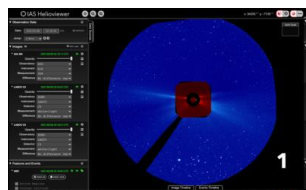
\includegraphics[width=0.48\linewidth]{2021_OBS-SKY_1-s1-panel1.pdf}\hfill
  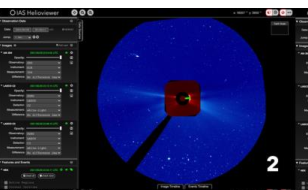
\includegraphics[width=0.48\linewidth]{2021_OBS-SKY_1-s1-panel2.pdf}\par\smallskip
  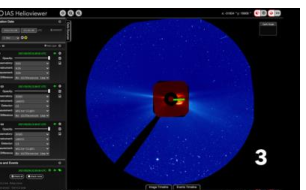
\includegraphics[width=0.48\linewidth]{2021_OBS-SKY_1-s1-panel3.pdf}\hfill
  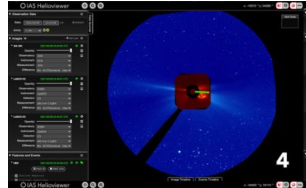
\includegraphics[width=0.48\linewidth]{2021_OBS-SKY_1-s1-panel4.pdf}\par\smallskip
  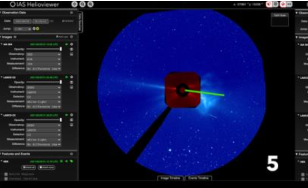
\includegraphics[width=0.48\linewidth]{2021_OBS-SKY_1-s1-panel5.pdf}\hfill
  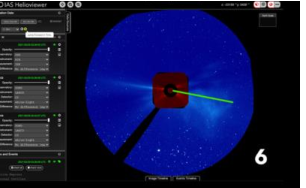
\includegraphics[width=0.48\linewidth]{2021_OBS-SKY_1-s1-panel6.pdf}\par\smallskip
  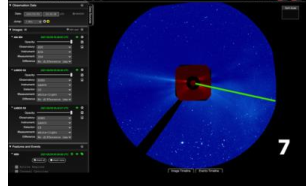
\includegraphics[width=0.48\linewidth]{2021_OBS-SKY_1-s1-panel7.pdf}
  \end{center}

  A total of 7 time intervals are selected tracing the evolution of the CME:
  \begin{enumerate}
  \item 2021/05/28 22:19:00 UT
  \item 2021/05/28 22:54:11 UT
  \item 2021/05/28 23:30:08 UT
  \item 2021/05/29 23:42:08 UT
  % sic: the official solution lists 2021/05/29 23:42:08 UT here, while its
  % summary table gives 2021/05/28 23:42:08 UT for interval 4
  \item 2021/05/29 01:12:16 UT
  \item 2021/05/29 03:36:08 UT
  \item 2021/05/29 05:00:08 UT
  % sic: the summary table gives 2021/05/29 05:36:08 UT for interval 7, but
  % 05:00:08 UT is consistent with the quoted 401 minutes from onset
  \end{enumerate}

  Summary of the information extracted from the images for all different
  selected intervals:

  {\footnotesize\setlength{\tabcolsep}{2.5pt}
  \begin{center}
  \begin{tabular}{c l c c c c c c}
  \toprule
  Interval & Date and Time & \begin{tabular}{@{}c@{}}Time\\ interval\\ (min)\end{tabular}
    & \begin{tabular}{@{}c@{}}Time from\\ CME onset\\ (min)\end{tabular}
    & \multicolumn{2}{c}{\begin{tabular}{@{}c@{}}Coordinates of\\ the CME front\end{tabular}}
    & \begin{tabular}{@{}c@{}}Distance from\\ disc center\\ (arcsec)\end{tabular}
    & \begin{tabular}{@{}c@{}}Distance from\\ disc center\\ (km)\end{tabular}\\
  & & & & $x''$ & $y''$ & &\\
  \midrule
  1 & 2021/05/28 22:19:00 UT & 0   & 0   & 950   & 144     & 961   & 696617\\
  2 & 2021/05/28 22:54:11 UT & 35  & 35  & 2682  & 174     & 2688  & 1948538\\
  3 & 2021/05/28 23:30:08 UT & 36  & 71  & 4579  & 97      & 4580  & 3320520\\
  4 & 2021/05/28 23:42:08 UT & 47  & 83  & 7441  & 116     & 7442  & 5395380\\
  5 & 2021/05/29 01:12:16 UT & 126 & 173 & 14000 & $-891$  & 14028 & 10170535\\
  6 & 2021/05/29 03:36:08 UT & 191 & 317 & 21048 & $-4570$ & 21538 & 15615349\\
  7 & 2021/05/29 05:36:08 UT & 210 & 401 & 27922 & $-7126$ & 28817 & 20892306\\
  \bottomrule
  \end{tabular}
  \end{center}
  % sic: the "Time interval" column of the official table is not consistent
  % with the differences of the successive timestamps (rows 4--7)

  \begin{center}
  \begin{tabular}{c c c c c c c}
  \toprule
  Interval & \begin{tabular}{@{}c@{}}Distance\\ from onset\\ (km)\end{tabular}
    & \begin{tabular}{@{}c@{}}Cumulative\\ velocity, plane\\ of the sky (km/s)\end{tabular}
    & \begin{tabular}{@{}c@{}}Deprojection of\\ velocity towards\\ ParkerSP (km/s)\end{tabular}
    & \begin{tabular}{@{}c@{}}Distance per\\ time interval\\ (km)\end{tabular}
    & \begin{tabular}{@{}c@{}}Velocity on\\ plane of the\\ sky (km/s)\end{tabular}
    & \begin{tabular}{@{}c@{}}Deprojection of\\ velocity towards\\ ParkerSP (km/s)\end{tabular}\\
  \midrule
  1 & 0        & 0   & 0    & 0       & 0   & 0\\
  2 & 1252198  & 596 & 728  & 1252198 & 596 & 728\\
  3 & 2624180  & 616 & 752  & 1371982 & 635 & 775\\
  4 & 4699040  & 944 & 1152 & 2074861 & 736 & 898\\
  5 & 9474195  & 913 & 1114 & 4775155 & 632 & 771\\
  6 & 14919009 & 784 & 958  & 5444814 & 475 & 580\\
  7 & 20195966 & 839 & 1025 & 5276957 & 419 & 511\\
  \bottomrule
  \end{tabular}
  \end{center}
  }
\item \textbf{Plotting the kinetic evolution of the CME.}

  Plots: distance vs time and velocity vs time.

  \ioaafig{2021_OBS-SKY_1-s2.pdf}
\item \textbf{Calculating the velocity of the CME front reaching ParkerSP.}

  The velocity corresponding to the last interval (up to reaching 30 solar
  radii) is 511\,km/s which, according to the considerations of the problem,
  would be the same velocity of the CME front once it reaches the ParkerSP.

  \textbf{Calculating the time spent by the CME front to reach the ParkerSP
  from its onset.}

  The Sun--ParkerSP distance estimated from Figure 1 is approx.\
  $0.66\,\mathrm{AU} = 9.9\times10^{7}\,\mathrm{km} = 141$ solar radii (given
  the information that 10 solar radii is approx.\ $7\times10^{6}$\,km).

  From the previous analysis, it is known that the CME front reaches a
  distance of 30 solar radii after 401 minutes (6.7 hours) from its onset
  (see Table). The distance that the CME travels at the constant speed of
  511\,km/s is expressed as $141-30=111$ solar radii
  $= 7.8\times 10^{7}$\,km, and thus the time spent in that interval is
  42.4 hours.

  Finally, the total time it takes for the CME front to reach the ParkerSP
  from its onset is computed as: $6.7 + 42.4 = 49.1$ hours.
\item \textbf{True and false statements}
  \begin{description}
  \item[A.] A larger number of selected images would give more precise
    information on the evolution of the CME and the calculated physical
    parameters. TRUE
  \item[B.] The analysis and measurements of the CME evolution should
    consider the differential rotation of the Sun, and therefore the
    calculated velocities will be affected. FALSE
  \item[C.] Any software (numerical) misalignment among the images when
    creating the mosaic will have direct effects on the precision of your
    calculations. TRUE
  \item[D.] The different assumptions made in order to construct the model
    displaying in a heliospheric density map in Figure 1, may affect the
    estimation of the Sun--ParkerSP distance. FALSE
  \item[E.] The interaction of the CME-front with the remnant dust left by
    the 2019 Borisov comet broadens and difuminate the images. This
    intensifies the lack of contrast in the images, increasing the
    uncertainty in determining the CME-front and its propagation. FALSE
    % sic: "difuminate" as in the original
  \end{description}
\item \textbf{Kinetic energy calculations}

  Proton:
  \[
  0.5 \times (1.67262\times10^{-27}~\mathrm{kg}) \times (511~\mathrm{m/s})^2
  = 1.4\times10^{-3}~\mathrm{eV}
  \]
  Alpha particle:
  \[
  0.5 \times (6.64\times10^{-27}~\mathrm{kg}) \times (511~\mathrm{m/s})^2
  = 5.4\times10^{-3}~\mathrm{eV}
  \]
  % sic: the official solution uses 511 m/s (instead of the CME speed of
  % 511 km/s); the quoted eV values follow from the m/s figure.
\end{enumerate}

\chapter{Optics, Telescopes \& Detectors}

\section*{Theory problems}

\probhead{5.1}{}{2007}{Chiang Mai, Thailand}{TH 1.13}{2}
% source id: 2007_TH_1.13   tag: naked-eye diffraction limit, lunar crater
A crater on the surface of the Moon has a diameter of 80\,km. Is it possible to
resolve this crater with naked eyes, assuming the eye pupil aperture is 5\,mm?

\probhead{5.2}{}{2008}{Bandung, Indonesia}{TH S10}{20}
% source id: 2008_TH_S10   tag: CCD frame fit and position angle
The coordinates of the components of Visual Binary Star $\mu$ Sco on August 22,
2008 are given in the table below.

\begin{center}
\begin{tabular}{|l|c|c|}
\hline
 & $\alpha$ (RA) & $\delta$ (Dec) \\
\hline
$\mu$ Sco 1 (primary) & $20^{\mathrm{h}}\,17^{\mathrm{m}}\,38^{\mathrm{s}}\!.90$
  & $-12^\circ\,30'\,30''$ \\
\hline
$\mu$ Sco 2 (secondary) &
  $20^{\mathrm{h}}\,18^{\mathrm{m}}\,03^{\mathrm{s}}\!.30$
  & $-12^\circ\,32'\,41''$ \\
\hline
\end{tabular}
\end{center}

The stars are observed using Zeiss refractor telescope at the Bosscha
Observatory with aperture and focal length are 600\,mm and 10\,780\,mm,
respectively. The telescope is equipped with $765 \times 510$ pixels CCD
camera. The pixel size of the chip is
$9\,\mu\mathrm{m} \times 9\,\mu\mathrm{m}$.

\begin{description}
\item[a.] Can both components of the binary be inside the frame? (``YES'' or
  ``NO'', show it in your computation!)
\item[b.] What is the position angle of the secondary star, with respect to the
  North?
\end{description}

\probhead{5.3}{}{2009}{Tehran, Iran}{TH P7}{10}
% source id: 2009_TH_P7   tag: eyepiece FOV from star drift time
A student tries to measure field of view (FOV) of the eyepiece of his/her
telescope, using rotation of the Earth. To do this job, the observer points the
telescope towards Vega (alpha Lyr., RA: $18.5^{\mathrm{h}}$, Dec: $+39^\circ$),
turns off its ``clock drive'' and measures trace out time, $t = 5.3$ minutes,
that Vega crosses the full diameter of the FOV. What is the FOV of this
telescope in arc-minutes?

\probhead{5.4}{}{2010}{Beijing, China}{TH S8}{10}
% source id: 2010_TH_S8   tag: VLBI wavelength to resolve Sgr A*
The Galactic Center is believed to contain a super-massive black hole with a
mass $M = 4 \times 10^6\,M_\odot$. The astronomy community is trying to resolve
its event horizon, which is a challenging task. For a non-rotating black hole,
this is the Schwarzschild radius, $R_s = 3(M/M_\odot)$\,km. Assume that we have
an Earth-sized telescope (using Very Long Baseline Interferometry). What
wavelengths should we adopt in order to resolve the event horizon of the black
hole? The Sun is located at 8.5\,kpc from the Galactic Center.

\probhead{5.5}{}{2010}{Beijing, China}{TH S9}{10}
% source id: 2010_TH_S9   tag: photon count rate, Gemini 8-m
A star has a measured I-band magnitude of 22.0. How many photons per second are
detected from this star by the Gemini Telescope (8\,m diameter)? Assume that
the overall quantum efficiency is 40\% and the filter passband is flat.

\begin{center}
\begin{tabular}{lccc}
Filter & $\lambda_0(\mathrm{nm})$ & $\Delta\lambda(\mathrm{nm})$
  & $F_{VEGA}(\mathrm{W\,m^{-2}\,nm^{-1}})$ \\
$I$ & $8.00 \times 10^2$ & 24.0 & $8.30 \times 10^{-12}$ \\
\end{tabular}
\end{center}

\probhead{5.6}{}{2011}{Katowice, Poland}{TH S5}{10}
% source id: 2011_TH_S5   tag: radio dish matching optical resolution
What would be the diameter of a radiotelescope working at a wavelength of
$\lambda = 1$\,cm with the same resolution as an optical telescope of diameter
$D = 10$\,cm?

\probhead{5.7}{}{2012}{Rio de Janeiro, Brazil}{TH S12}{}
% source id: 2012_TH_S12   tag: telescope to resolve Earth's lunar wobble
What is the minimum diameter of a telescope, observing in the visible and near
ultraviolet bands, located in one of the Lagrangian points L4 or L5 of the
Sun--Earth system, in order to be able to detect the Earth's wobbling relative
to the ecliptic plane caused by the gravitational action of the Moon?

\probhead{5.8}{}{2013}{Volos, Greece}{TH S2}{10}
% source id: 2013_TH_S2   tag: telescope diameter to resolve hot Jupiter
Let us assume that we observe a hot Jupiter planet orbiting around a star at an
average distance $d = 5$\,AU. It has been found that the distance of this
system from us is $r = 250$\,pc. What is the minimum diameter, $D$, that a
telescope should have to be able to resolve the two objects (star and planet)?
We assume that the observation is done in the optical part of the
electromagnetic spectrum ($\lambda \sim 500$\,nm), outside the Earth's
atmosphere and that the telescope optics are perfect.

\probhead{5.9}{The Vega star in the mirror}{2014}{Suceava, Romania}{TH P12}{}
% source id: 2014_TH_P12   tag: double image photometry with mirror
Inside a photo camera a plane mirror is placed along the optical axis of the
lens of the objective (as seen in figure below). The length of the mirror is
half of the focal distance of the lens of the objective. The photo camera is
oriented as on the photographic plate situated in the focal plane of the photo
camera are captured two images with different illuminations of the Vega star.
Find out the difference between the apparent photographical magnitudes of the
two images of the Vega stars.

\ioaafig{2014_TH_P12-f1.pdf}
% Vega starlight entering a lens objective (aperture r), a plane mirror of
% length f/2 lying on the optical axis in front of the photographic plate at
% focal distance f, with the two image positions Sigma_1 and Sigma_2 separated
% by r/2 on the plate. No auto-extracted figure exists for 2014_TH_P12.

\probhead{5.10}{}{2015}{Magelang, Indonesia}{TH S4}{}
% source id: 2015_TH_S4   tag: resolving supermassive black hole
Let us assume that an observer using a hypothetical, far-infrared, Earth-sized
telescope (wavelength range 20 to 640\,$\mu$m) found a static and neutral
supermassive black hole with a mass of $2.1 \times 10^{10}\,\mathrm{M}_\odot$.
Determine the maximum distance at which this black hole can be resolved by the
observer.

\probhead{5.11}{AstroSat}{2016}{Bhubaneswar, India}{TH T12}{50}
% source id: 2016_TH_T12   tag: X-ray instrument count rates, SNR
India astronomy satellite, AstroSat, launched in September 2015, has five
different instruments.

\ioaafig{2016_TH_T12-f1.pdf}

In this question, we will discuss three of these instruments (SXT, LAXPC,
CZTI), which point in the same direction and observe in X-ray wavelengths. The
details of these instruments are given in the table below.

\begin{center}
\small
\begin{tabular}{|l|c|c|c|p{3.2cm}|c|}
\hline
Instrument & Band & Collecting & Effective Photon & Saturation level & No.\ of
\\
 & [keV] & Area [m$^2$] & Detection Efficiency & [counts] & Pixels \\
\hline
SXT & 0.3--80 & 0.067 & 60\% & 15000 (total) & $512 \times 512$ \\
\hline
LAXPC & 3--80 & 1.5 & 40\% & 50000 (in any one counter) or 200000 (total)
  & --- \\
\hline
CZTI & 10--150 & 0.09 & 50\% & --- & $4 \times 4096$ \\
\hline
\end{tabular}
\end{center}

You should note that LAXPC energy range is divided into 8 different energy band
counters of equal bandwidth with no overlap.

\begin{description}
\item[(T12.1)] Some X-ray sources like Cas A have a prominent emission line at
  0.01825\,nm corresponding to a radioactive transition of $^{44}$Ti. Suppose
  there exists a source which emits only one bright emission line corresponding
  to this transition. What should be the minimum relative velocity ($v$) of the
  source, which will make the observed peak of this line to get registered in a
  different energy band counter of LAXPC as compared to a source at rest?
\end{description}

These instruments were used to observe an X-ray source (assumed to be a point
source), whose energy spectrum followed the power law,
\[ F(E) = K E^{-2/3} \qquad
   [\text{in units of counts/keV/m}^2\text{/s}] \]
where $E$ is the energy in keV, $K$ is a constant and $F(E)$ is photon flux
density at that energy. Photon flux density, by definition, is given for per
unit collecting area (m$^2$) per unit bandwidth (keV) and per unit time
(seconds). From prior observations, we know that the source has a flux density
of 10\,counts/keV/m$^2$/s at 1\,keV, when measured by a detector with 100\%
photon detection efficiency. The ``counts'' here mean the number of photons
reported by the detector.

As the source flux follows the power law given above, we know that for a given
energy range from $E_1$ (lower energy) to $E_2$ (higher energy) the total
photon flux ($F_{\mathrm{T}}$) will be given by
\[ F_{\mathrm{T}} = 3K\left(E_2^{1/3} - E_1^{1/3}\right) \qquad
   [\text{in units of counts/m}^2\text{/s}] \]

\begin{description}
\item[(T12.2)] Estimate the incident flux density from the source at 1\,keV,
  5\,keV, 40\,keV and 100\,keV. Also estimate what will be the total count per
  unit bandwidth recorded by each of the instruments at these energies for an
  exposure time of 200 seconds.
\item[(T12.3)] For this source, calculate the maximum exposure time
  ($t_{\mathrm{S}}$), without suffering from saturation, for the CCD of SXT.
\item[(T12.4)] If the source became 3500 times brighter, calculate the expected
  counts per second in LAXPC counter 1, counter 8 as well as total counts
  across the entire energy range. If we observe for longer period, will the
  counter saturate due to any individual counter or due to the total count?
  Tick the appropriate box in the Summary Answersheet.
\item[(T12.5)] Assume that the counts reported by CZTI due to random
  fluctuations in electronics are about 0.00014 counts per pixel per keV per
  second at all energy levels. Any source is considered as ``detected'' when
  the SNR (signal to noise ratio) is at least 3. What is minimum exposure time,
  $t_c$, needed for the source above to be detected in CZTI?\\
  Note that the ``noise'' in a detector is equal to the square root of the
  counts due to random fluctuations.
\item[(T12.6)] Let us consider the situation where the source shows variability
  in number flux, so that the factor $K$ increases by 20\%. AstroSat observed
  this source for 1 second before the change and 1 second after this change in
  brightness. Calculate the counts measured by SXT, LAXPC and CZTI in both the
  observations. Which instrument is best suited to detect this change? Tick the
  appropriate box in the Summary Answersheet.
\end{description}

\probhead{5.12}{GMRT beam transit}{2016}{Bhubaneswar, India}{TH T5}{10}
% source id: 2016_TH_T5   tag: source transit through radio dish FWHM
Giant Metrewave Radio Telescope (GMRT), one of the world's largest radio
telescopes at metre wavelengths, is located in western India (latitude:
$19^\circ 6'$\,N, longitude: $74^\circ 3'$\,E). GMRT consists of 30 dish
antennas, each with a diameter of 45.0\,m. A single dish of GMRT was held fixed
with its axis pointing at a zenith angle of $39^\circ 42'$ along the northern
meridian such that a radio point source would pass along a diameter of the
beam, when it is transiting the meridian.

What is the duration $T_{\mathrm{transit}}$ for which this source would be
within the FWHM (full width at half maximum) of the beam of a single GMRT dish
observing at 200\,MHz?

\textbf{Hint:} The FWHM size of the beam of a radio dish operating at a given
frequency corresponds to the angular resolution of the dish. Assume uniform
illumination.

\probhead{5.13}{Telescope optics}{2016}{Bhubaneswar, India}{TH T7}{20}
% source id: 2016_TH_T7   tag: magnification, Barlow lens, CCD pixel scale
In a particular ideal refracting telescope of focal ratio $f/5$, the focal
length of the objective lens is 100\,cm and that of the eyepiece is 1\,cm.

\begin{description}
\item[(T7.1)] What is the angular magnification, $m_0$, of the telescope? What
  is the length of the telescope, $L_0$, i.e.\ the distance between its
  objective and eyepiece?
\end{description}

An introduction of a concave lens (Barlow lens) between the objective lens and
the prime focus is a common way to increase the magnification without a large
increase in the length of the telescope. A Barlow lens of focal length 1\,cm is
now introduced between the objective and the eyepiece to double the
magnification.

\begin{description}
\item[(T7.2)] At what distance, $d_{\mathrm{B}}$, from the prime focus must the
  Barlow lens be kept in order to obtain this desired double magnification?
\item[(T7.3)] What is the increase, $\Delta L$, in the length of the telescope?
\end{description}

A telescope is now constructed with the same objective lens and a CCD detector
placed at the prime focus (without any Barlow lens or eyepiece). The size of
each pixel of the CCD detector is 10\,$\mu$m.

\begin{description}
\item[(T7.4)] What will be the distance in pixels between the centroids of the
  images of the two stars, $n_{\mathrm{p}}$, on the CCD, if they are $20''$
  apart on the sky?
\end{description}

\probhead{5.14}{U-Band photometry}{2016}{Bhubaneswar, India}{TH T8}{20}
% source id: 2016_TH_T8   tag: photon counting, sky background
A star has an apparent magnitude $m_{\mathrm{U}} = 15.0$ in the $U$-band. The
$U$-band filter is ideal, i.e., it has perfect (100\%) transmission within the
band and is completely opaque (0\% transmission) outside the band. The filter
is centered at 360\,nm, and has a width of 80\,nm. It is assumed that the star
also has a flat energy spectrum with respect to frequency. The conversion
between magnitude, $m$, in any band and flux density, $f$, of a star in Jansky
($1\,\mathrm{Jy} = 1 \times 10^{-26}\,\mathrm{W\,Hz^{-1}\,m^{-2}}$) is given by
\[ f = 3631 \times 10^{-0.4 m}\,\mathrm{Jy} \]

\begin{description}
\item[(T8.1)] Approximately how many $U$-band photons, $N_0$, from this star
  will be incident normally on a $1\,\mathrm{m}^2$ area at the top of the
  Earth's atmosphere every second?
\end{description}

This star is being observed in the $U$-band using a ground based telescope,
whose primary mirror has a diameter of 2.0\,m. Atmospheric extinction in
$U$-band during the observation is 50\%. You may assume that the seeing is
diffraction limited. Average surface brightness of night sky in $U$-band was
measured to be 22.0\,mag/arcsec$^2$.

\begin{description}
\item[(T8.2)] What is the ratio, $R$, of number of photons received per second
  from the star to that received from the sky, when measured over a circular
  aperture of diameter $2''$?
\item[(T8.3)] In practice, only 20\% of $U$-band photons falling on the primary
  mirror are detected. How many photons, $N_{\mathrm{t}}$, from the star are
  detected per second?
\end{description}

\probhead{5.15}{GOTO}{2017}{Phuket, Thailand}{TH T10}{25}
% source id: 2017_TH_T10   tag: plate scale, CCD noise, SNR, exposure
The Gravitational-Wave Optical Transient Observer (GOTO) aims to carry out
searches of optical counterparts of any Gravitational Wave (GW) sources within
an hour of their detection by the LIGO and VIRGO experiments. The survey needs
to cover a big area on the sky in a short time to search all possible regions
constrained by the GW experiments before the optical burst signal, if any,
fades away. The GOTO telescope array is composed of 4 identical reflective
telescopes, each with 40-cm diameter aperture and f-ratio of 2.5, working
together to image large regions of the sky. For simplicity, we assume that the
telescopes' fields-of-view (FoV) do not overlap with one another.

\begin{description}
\item[a)] Calculate the projected angular size per mm at the focal plane, i.e.\
  plate scale, of each telescope. \hfill[6]
\item[b)] If the zero-point magnitude (i.e.\ the magnitude at which the count
  rate detected by the detector is 1 count per second) of the telescope system
  is 18.5\,mag, calculate the minimum time needed to reach 21\,mag at
  Signal-to-Noise Ratio (SNR) $= 5$ for a point source. We first assume that
  the noise is dominated by both the Read-Out Noise (RON) at 10 counts/pixel
  and the CCD dark (thermal) noise (DN) rate of 1 count/pix/minute. The CCDs
  used with the GOTO have a 6-micron pixel size and gain (conversion factor
  between photo-electron and data count) of 1. The typical seeing at the
  observatory site is around 1.0\,arcsec. \hfill[8]\\
  The Signal-to-Noise Ratio is defined as
  \[ \mathrm{SNR} \equiv
     \frac{\text{Total Source Count}}{\sqrt{\sum_i \mathrm{Noise}_i^2}}
     = \frac{\text{Total Source Count}}
            {\sqrt{\sigma_{\mathrm{RON}}^2 + \sigma_{\mathrm{DN}}^2 + \dots}},
  \]
  \[ \sigma_{\mathrm{RON}} = \sqrt{N_{\mathrm{pix}} \cdot \mathrm{RON}^2},
     \qquad
     \sigma_{\mathrm{DN}} = \sqrt{N_{\mathrm{pix}} \cdot \mathrm{DN} \cdot t},
  \]
  where $t$ is the exposure time.
\item[c)] Normally when the exposure time is long and the source count is high
  then Poisson noise from the source is also significant. Determine the
  relation between SNR and exposure time in the case that the noise is
  dominated by Poisson noise of the source. Recalculate the minimum exposure
  time required to reach 21\,mag with SNR $= 5$ from part b) if Poisson noise
  is also taken into consideration. The Poisson noise (standard deviation) of
  the source is given by
  $\sigma_{\mathrm{source}} = \sqrt{\text{Source Count}}$. In reality, there is
  also the sky background which can be important source of Poisson noise. For
  our purpose here, please ignore any sky background in the calculation.
  \hfill[6]
\item[d)] The typical localisation uncertainty of the GW detector is about 100
  square-degrees and we would like to cover the entire possible location of any
  candidate within an hour after the GW is detected. Estimate the minimum side
  length of the square CCD needed for each telescope in terms of the number of
  pixels. You may assume that the time taken for the CCD read-out and the
  pointing change are negligible. \hfill[5]
\end{description}

\probhead{5.16}{Radio Galaxy}{2018}{Beijing, China}{TH T9}{25}
% source id: 2018_TH_T9   tag: radiometer equation, integration time
An observer wants to use the Five-hundred-meter Aperture Spherical radio
Telescope (FAST) in China to observe a radio galaxy at redshift of $z = 0.06$.
We assume that the radio source is compact compared to the beam size of the
telescope at the observing frequencies, i.e., the source is point-like as seen
through the telescope. To detect a point source with FAST, it must be
sufficiently strong (bright) relative to the noise level (for single
polarization observations), $\sigma$, which depends on the bandwidth,
$\Delta\nu$, and the integration time (the radio astronomy equivalent of
exposure time), $t_i$, as follows:
\[ \sigma = \frac{2 k_B T_{sys}}{A_e \sqrt{t_i\,\Delta\nu}} \]
where $T_{sys}$ is the system temperature (about 150\,K in the frequency range
of 0.28\,GHz -- 0.56\,GHz and 25\,K in the frequency range of 1.05\,GHz --
1.45\,GHz), and $A_e = 4.6 \times 10^4\,\mathrm{m}^2$ is the effective area of
the telescope taking into account the total efficiency of the instrument.

This radio galaxy has an observed continuum flux density of
$f_\nu = 2.5 \times 10^{-3}$\,Jy at an observing frequency of 0.4\,GHz. The
bandwidth $\Delta\nu$ for the continuum observation centered at 0.4\,GHz is
$2.8 \times 10^8$\,Hz.

\begin{description}
\item[(a)] In order to detect the continuum flux density at 0.4\,GHz with a
  signal-to-noise ratio of 30 (a so-called 30$\sigma$ detection), what is the
  required integration time, $t_i$?
\item[(b)] We want to search for the neutral Hydrogen (HI) in the galaxy using
  21\,cm absorption line. The HI 21\,cm line, with rest frame frequency of
  1.4204\,GHz. Calculate the observed frequency ($\nu_{obs}$) of the HI line
  for this galaxy.
\item[(c)] The radio continuum emission from this galaxy can be described by a
  power law $f_\nu \sim \nu^\alpha$, with a spectral index of $\alpha = -0.2$.
  Calculate the continuum flux density at $\nu_{obs}$ for this galaxy.
\item[(d)] The line width of the HI 21\,cm absorption line is 90\,km/s.
  Calculate the line width in Hz at the observing frequency of $\nu_{obs}$.
  According to Figure 1, the HI 21\,cm line absorbs 4\% of the continuum flux
  density (on average) over the line width of 90\,km\,s$^{-1}$. In order to
  detect the absorption line at $\geq 3\sigma$ in three consecutive
  30\,km\,s$^{-1}$ channels, what is the required integration time?
\end{description}

% Figure 1: spectrum of the HI 21cm absorption relative to the continuum
% emission in the radio galaxy.
\ioaafig{2018_TH_T9-f1.pdf}

\probhead{5.17}{Photographing a nanosatellite}{2019}{Keszthely, Hungary}{TH 14}{60}
% source id: 2019_TH_14   tag: cubesat magnitude, CCD detection, trailing
The very first, entirely Hungarian-made, satellite was ``MASAT--1'', a
nanosatellite ``cubesat''. It was made mostly of aluminium with total mass
1\,kg, sides length $l = 10$\,cm and a longer communication aerial. It was
designed and prepared at the Technical University of Budapest (BME) in 2009 by
students. The launch occurred on February 13, 2012, using a Vega rocket from
the Kourou launch site --- together with several other cubesats from other
countries. It operated successfully right up to the last minutes of its
lifetime (the transmitted last data packages were captured by radio receivers
on the evening of January 9, 2015, a few hours later the nanosatellite
re-entered the atmosphere and disintegrated).

\ioaafig{2019_TH_14-f1.pdf}

The orbital altitude of MASAT--1 changed between $h_{\mathrm{min}} = 350$\,km
and $h_{\mathrm{max}} = 1450$\,km (due to its highly eccentric orbit), but in
this question assume it to be in a circular orbit 900\,km above the sea level.

The MASAT team wished to photograph their nanosatellite from the ground. Thus,
they called the staff of Baja Astronomical Observatory (South Hungary,
$\lambda_{\mathrm{B}} = 19.010843^\circ$,
$\varphi_{\mathrm{B}} = 46.180329^\circ$, $h_{\mathrm{B}} = 100$\,m) to
photograph the orbiting MASAT--1 with their telescope.

The observatory has a Ritchey-Chr\'etien type reflecting telescope with a
diameter of 50\,cm, and focal ratio of $f/8.4$. The CCD camera installed on the
telescope had a $4096 \times 4096$ chip with 9\,$\mu$m sized square pixels. The
quantum efficiency of the CCD was about 70\,\%. The practical detection limit
was about $19.5^{\mathrm{m}}$ visual band applying a
$\tau_{\mathrm{exp}} = 2$\,min exposure time. Disregard any effects of seeing.
The orbital inclination of MASAT--1 was about $i = 70^\circ$ and the direction
of the orbital motion was the same as the Earth rotation. In addition, let us
assume that the reflection area always is 100\,cm$^2$. Throughout this event,
the telescope was pointed to the local zenith, and its RA motor was tracking
the stars. Consider only light from the Sun, you can ignore light reflected
from Earth and Moon. Ignore the effects of atmospheric extinction.

\begin{description}
\item[a)] Calculate the apparent visual magnitude of this cubesat under ideal
  observational circumstances, i.e.\ when it was at the local zenith of the
  observing site (Baja, Hungary) at midnight. Omit all atmospheric effects, and
  consider the Earth to be a sphere. The albedo of a specular aluminium plate
  is $a \approx 0.70$. \hfill(10\,p)\\
  \textit{Hint:} Use a comparison of MASAT--1 with the Full Moon.
\item[b)] What was the Observatory's answer to the MASAT team; would it ever be
  possible to photograph their nanosatellite with the existing equipment at the
  observatory? \textbf{Mark ``YES'' or ``NO'' on the answer sheet.} Support
  your answer with detailed calculations. \hfill(42\,p)
\item[c)] What would have been the answer if they had taken into account the
  blurring effect of the atmosphere, the so-called seeing? In Hungary the
  typical FWHM (Full Width at Half Maximum) value of the blurred stellar images
  --- which can be approximated by a symmetric 2D Gaussian profile close to the
  zenith --- is about $3.5''$. \textbf{Mark ``YES'' or ``NO'' or ``Close to the
  limit'' on the answer sheet.} Support your answer with a short calculation.
  \hfill(8\,p)\\
  \textit{Hint:} Although the illumination of the seeing spot in the focal
  plane can be approximated by a symmetric 2D Gaussian profile, you can take it
  to be homogeneous in your calculation.
\end{description}

\probhead{5.18}{Improving a common reflecting telescope}{2019}{Keszthely, Hungary}{TH 4}{10}
% source id: 2019_TH_4   tag: mirror reflectivity, limiting-magnitude gain
A student has an average quality Cassegrain telescope, with primary and
secondary mirrors having $\varepsilon_1 = 91$\,\% reflectivity aluminium
layers.

\begin{description}
\item[a)] What will be the change in the limiting magnitude of this telescope
  by replacing the mirror coatings with ``premium'' quality
  $\varepsilon_2 = 98$\,\% reflectivity ones? \hfill(5\,p)
\item[b)] Assuming the student also uses a star diagonal mirror, also with
  reflectivity $\varepsilon_1$ with the original telescope --- what will be the
  improvement if he/she also replaces this piece with an
  $\varepsilon_3 = 99$\,\% reflectivity (``dielectric'' mirror) model, combined
  with the new $\varepsilon_2$ mirrors? \hfill(3\,p)\\
  (A star diagonal mirror is a flat mirror, inclined to the optical axis by
  $45^\circ$.)
\item[c)] Is this difference obviously detectable by the human eye? \textbf{
  Mark ``YES'' or ``NO'' on the answer sheet.} \hfill(2\,p)
\end{description}

Consider the whole visual band and disregard any wavelength dependence and
geometric effects.

\probhead{5.19}{Astrophotography}{2020}{GeCAA (Estonia, remote)}{TH 1}{10}
% source id: 2020_TH_1   tag: camera FOV, pixel scale, star trails
An astrophotographer, based on the Equator, uses a good digital camera on a
tripod, but with no tracking. The camera has a telescopic lens with focal
length of 150\,mm and aperture (objective diameter) of 84\,mm. The sensor has
effective light collecting diameter of 22.5\,mm. The photographic target is a
star field at the observer's Zenith.

\begin{description}
\item[(a)] Calculate the field of view (the angular width of the image) which
  can be captured on the sensor using this equipment. \hfill(2 points)
\item[(b)] The pixels in the camera's sensor are separated by a distance of
  $3.23\,\mu$m. What is the maximum possible exposure time for a single
  frame, so that no star trails appear on the exposed image?
  \hfill(5 points)
\item[(c)] For a better-quality image of the star field, the photographer
  decides to take multiple shots at the exposure time calculated in b) and
  then to stack them together. The total time for all these shots is 30\,s
  (ignore any time taken to write data to the memory card) What proportion of
  the total field of view is possible at the higher signal to noise ratio?
  \hfill(3 points)
\end{description}

\probhead{5.20}{Lucy: The First Mission to the Trojan Asteroids}{2021}{Bogot\'a (remote)}{TH Q13}{15}
% source id: 2021_TH_Q13   tag: CCD radiation noise, excited pixels
CCD cameras on space probes are very sensitive and exposed to space weather
conditions. Intense radiation passing through the CCD produces electron-hole
pairs in the silicon of the CCD chip. The rate at which these pairs are
produced is an important parameter when operating cameras on board spacecraft
and can be calculated for radiation of any given energy.

A high energy particle or photon of radiation passing through the CCD will
deposit some energy in the chip with each electron-hole pair it creates. The
`stopping power' of silicon for a given type of particle can be measured as
the energy per areal density ($\mathrm{areal\ density} = \mathrm{mass\ per\
unit\ area}$) that the silicon `takes away' from the travelling particle.

\ioaafig{2021_TH_Q13-f1.pdf}

NASA's Lucy mission will be the first to study the Trojan asteroids and will
revolutionize our understanding of the formation of the Solar System. One of
the instruments on board is L'LORRI (Lucy LOng Range Reconnaissance Imager),
which contains a sensitive CCD in order to produce detailed images of the
Trojan asteroids. Unfortunately, the radiation around Jupiter is very intense
and it can generate a lot of `noise' in the pixels of the CCD.

Let us assume that an average charged particle trapped in Jupiter's magnetic
field has an energy of 15\,MeV and that the flux of such particles in this
region is equivalent to about 600 electrons $\mathrm{s}^{-1}\,
\mathrm{cm}^{-2}$. Also assume that for each electron-hole pair which a
particle passing through a pixel creates, it deposits exactly the excitation
energy of the pair in that pixel. After the pixel crosses a threshold number
of electron-hole pairs it is `excited' and no more pairs can be produced in
that pixel. Any remaining energy in the particle is passed to the next pixel
(and so on).

Using the data given below for the CCD chip in the L'LORRI camera, answer the
following questions:

\begin{description}
\item[(13.1)] How many pixels will be excited by one such particle of
  radiation passing through the CCD when the spacecraft is near Jupiter's
  orbit? \hfill[10.0\,pt]
\item[(13.2)] Given the radiation flux near Jupiter, what percentage of the
  total number of pixels in an image will be excited? \hfill[5.0\,pt]
\end{description}

CCD Data:
\begin{itemize}
\item Exposure time of an image $= 30$\,ms
\item Pixels on the CCD $= 1024 \times 1024$
\item CCD Area $= 13\,\mathrm{mm} \times 13\,\mathrm{mm}$
\item CCD chip thickness $= 0.06$\,cm
\item Density of silicon, $\rho = 2.34\,\mathrm{g\,cm}^{-3}$
\item Excitation energy of single pair $= 2.36$\,eV
\item Excitation threshold of a single pixel $= 250$ pairs
\item `Stopping power' of silicon for a 15\,MeV electron
  $= 3.012\,\mathrm{MeV\,g}^{-1}\,\mathrm{cm}^{2}$
\end{itemize}

\probhead{5.21}{ALMA - Calculating photons}{2021}{Bogot\'a (remote)}{TH Q4}{10}
% source id: 2021_TH_Q4   tag: photon rates, interferometer resolution
ALMA is a radio observatory with a revolutionary design. It consists of 66
high-precision antennas, operating in the wavelength range from 0.32\,mm to
8.60\,mm. The principal array has fifty antennas of 12\,m diameter each that
can work together as a single telescope in the so-called interferometric
mode. There is also another array of four 12\,m antennas, and twelve smaller
antennas of 7\,m diameter each.

Imagine that a single 12\,m antenna is being calibrated, pointing to a source
with a known incident flux of $1 \times 10^{-20}\,\mathrm{W/m}^2$.

\begin{description}
\item[(4.1)] Assuming that all the flux arrives at the shortest wavelength of
  ALMA sensitivity, determine the average number of photons that would reach
  the detector every second. \hfill[2.0\,pt]
\item[(4.2)] Compare it to the average number of photons that would have
  reached the detector, if all the flux arrived at the longest wavelength of
  operation. \hfill[2.0\,pt]
\item[(4.3)] What is the angular resolution (in arcsec) of a single 12\,m
  antenna, operating at 74.9\,GHz? \hfill[2.0\,pt]
\item[(4.4)] Imagine the principal array operating at 74.9\,GHz in the
  interferometric mode. Assuming for simplicity that the spatial resolution
  is solely given by the longest baseline (largest distance between any pair
  of antennas), which turns to be $D_{\max} = 16$\,km, what would be the
  angular resolution (in arcsec) in this case? Treat this case as a single
  slit aperture instead of a circular one. \hfill[2.0\,pt]
\item[(4.5)] For a radio antenna, the term SEFD refers to `System Equivalent
  Flux Density', which is a characteristic energy flux density of the
  antenna, depending on its temperature and size. We also note that for
  energy estimation of radio photons, Rayleigh-Jeans approximation is valid.
  Assuming a system temperature of 691\,K, what would be the SEFD of the full
  ALMA observatory in Jansky if all the 66 antennas could work together?
  \hfill[2.0\,pt]
\end{description}

\probhead{5.22}{Microlensing}{2023}{Katowice, Poland}{TH Q3}{5}
% source id: 2023_TH_Q3   tag: telescope diameter for equal S/N
A faint subdwarf star ($I = 20.4$\,mag) in the Galactic bulge was observed to
brighten to $I' = 15.2$\,mag as a result of gravitational microlensing,
allowing a high-resolution spectrum to be obtained with the UVES spectrograph
on the Very Large Telescope (mirror diameter $D = 8.2$\,m).

Estimate the diameter of the telescope needed to obtain a spectrum of the
same quality with the same instrument and exposure time for this star at its
normal apparent brightness. The fiber aperture is small enough so that the
sky background is negligible.

\probhead{5.23}{Bolometer}{2023}{Katowice, Poland}{TH Q6}{13}
% source id: 2023_TH_Q6   tag: conical cavity absorption, effective temperature
The entrance cavity of a particular bolometer is a cone with an opening angle
of $30^\circ$, the surface of which has an energy absorption coefficient of
$a = 0.99$. Assume that there is no scattering of the incident radiation on
the walls of the cavity, only multiple mirror-like (specular) reflections.
The bolometer is connected to a cooler which keeps the bolometer cavity
surface at practically 0\,K temperature. The instrument is orbiting at 2\,au
from the Sun and is pointed directly at the centre of the Solar disk.

Calculate the temperature of a black body which would radiate the same
amount of energy as the entire bolometer opening does per unit surface area.

Note: the opening angle is defined as twice the angle between the axis of
the cone and its generatrix.

\probhead{5.24}{Cluster Photography}{2024}{Rio de Janeiro, Brazil}{TH T6}{20}
% source id: 2024_TH_T6   tag: plate scale, CCD signal-to-noise
An astronomer takes pictures, in the $V$-band, of a faint celestial target,
from a place with no light pollution. The selected target is the globular
cluster Palomar 4, which has an angular diameter of $\theta = 72.0''$ and a
uniform surface brightness in the $V$-band of $m_V = 20.6$\,mag/arcsec$^2$.
The observation equipment consists of one reflector telescope, with diameter
$D = 305$\,mm and f-ratio $f/5$, and a prime focus CCD with quantum
efficiency $\eta = 80\%$ and square pixels with size $\ell = 3.80\,\mu$m.

Given data:
\begin{itemize}
\item $V$-band central wavelength: $\lambda_V = 550$\,nm
\item $V$-band bandwidth: $\Delta\lambda_V = 88.0$\,nm
\item Photon flux for a 0-magnitude object in the $V$-band:
  $10000\,\mathrm{counts/nm/cm^2/s}$
\end{itemize}

\begin{description}
\item[(a)] Calculate the plate scale (the angle of sky projected per unit
  length of the sensor) of the observation equipment in arcmin/mm.
  \hfill(3 points)
\item[(b)] Estimate the number of pixels, $n_p$, covered by the cluster
  image on the CCD. \hfill(4 points)
\item[(c)] With an exposure time of $t = 15$ seconds, the astronomer obtains
  a signal-to-noise ratio of $S/N = 225$. Compute the brightness of the sky
  at the observation site, knowing that the CCD has a readout noise
  (standard deviation) of 5 counts per pixel and dark noise of 6 counts per
  pixel per minute. Give your answer in mag/arcsec$^2$. You may find useful:
  $\sigma^2_{RON} = n_p \cdot 1 \cdot RON^2$ and
  $\sigma^2_{DN} = n_p \cdot DN \cdot t$. \hfill(13 points)
\end{description}

\probhead{5.25}{Daksha Mission}{2025}{Mumbai, India}{TH T01}{10}
% source id: 2025_TH_T01   tag: detector geometry, timing localization
``Daksha'' is a proposed Indian mission consisting of two satellites S1 and
S2 orbiting the Earth in the same circular orbit of radius $r = 7000$\,km but
with $180^\circ$ phase difference. These satellites observe the universe in
high energy domain (X-rays and $\gamma$-rays). Each of the satellites of
Daksha uses several flat, rectangular detectors.

To understand how to localize a source in the sky, we shall use a simplified
model of the Daksha mission. Assume that S1 has only two identical detectors
D1 and D2, each of area $A = 0.50\,\mathrm{m}^2$, attached to an opaque mount
M as shown in the figure below. The detectors lie symmetrically around the
$y$ axis in planes perpendicular to the $x$-$y$ plane and make an angle
$\alpha = 120^\circ$ with each other.

\ioaafig{2025_TH_T01-f1.pdf}

\begin{description}
\item[(T01.1)] When observing a distant source located in the $x$-$y$ plane,
  detector D1 records a power $P_1 = 2.70 \times 10^{-10}\,\mathrm{J\,s}^{-1}$
  and detector D2 records a power
  $P_2 = 4.70 \times 10^{-10}\,\mathrm{J\,s}^{-1}$. Estimate the angle $\eta$
  made by the position vector of the source with the positive $y$-axis, with
  counter-clockwise angle from the positive $y$ axis being considered
  positive. \hfill[5]
\end{description}

Consider a single pulse from a distant source (not necessarily in the
$x$-$y$ plane) recorded by both satellites (S1 and S2) of Daksha. The times
of the peaks of the pulses recorded by S1 and S2 are $t_1$ and $t_2$,
respectively.

\begin{description}
\item[(T01.2)] If $t_1 - t_2$ was measured to be $10.0 \pm 0.1$\,ms then
  determine the fraction, $f$, of the celestial sphere where the source
  might lie. \hfill[5]
\end{description}

\probhead{5.26}{Atmospheric Seeing}{2025}{Mumbai, India}{TH T09}{35}
% source id: 2025_TH_T09   tag: refraction layers, speckles
A telescope with an achromatic convex objective lens of diameter
$D = 15$\,cm and focal length $f = 200$\,cm is pointed to a star at the
zenith.

\begin{description}
\item[(T09.1)] Find the diameter (in m), $d_{\mathrm{image}}$, of the image
  of a point source as produced by the objective lens at its focal plane for
  green light ($\lambda = 550$\,nm), considering only the effects of
  diffraction. \hfill[1]
\end{description}

The image of an astronomical source is also affected by the so-called
``atmospheric seeing''. The boundaries between the layers in the atmosphere
as well as the refractive indices of the layers change continuously due to
turbulence, temperature variation and other factors. This leads to tiny
changes in the position of the image in the focal plane of the telescope,
known as the ``twinkling effect''. For rest of the problem, apart from the
diffraction limited finite size of the image of the star discussed above, no
interference effects will be considered.

The left panel of the figure below shows a vertical cross-section of the
atmosphere with multiple layers of different refractive indices
($n_1, n_2, n_3, \ldots$). The right panel shows the zoomed in view of a
thin vertical segment of the atmosphere and the boundary between the two
lowest atmospheric layers of refractive indices $n_1$ and $n_2$
($n_1 > n_2$). We consider only these two layers and their boundary for this
problem. The diagrams are not to scale.

\ioaafig{2025_TH_T09-f1.pdf}

\begin{description}
\item[(T09.2)] Let the boundary between the two layers be at a height
  $H = 1$\,km directly above the telescope objective, with a tilt of
  $\theta = 30^\circ$ with respect to the horizontal plane. In all parts of
  this problem $\theta$ is taken to be positive in the anti-clockwise
  direction. For a monochromatic light source, $n_1 = 1.00027$ and
  $n_2 = 1.00026$. Let the angular shift in the position of the image at the
  focal plane of the telescope for a star at the zenith be $\alpha$.
  \begin{description}
  \item[(T09.2a)] Draw an appropriately labelled ray-diagram at the boundary
    showing $n_1$, $n_2$, $\theta$ and $\alpha$. \hfill[2]
  \item[(T09.2b)] Find the expression for $\alpha$ in terms of $\theta$,
    $n_1$ and $n_2$. Use the small angle approximations:
    $\sin\alpha \approx \alpha$ and $\cos\alpha \approx 1$. \hfill[2]
  \item[(T09.2c)] Calculate the displacement, $\Delta x_\theta$ (in m), in
    the position of the image if $\theta$ increases by 1\% (keeping $n_1$
    and $n_2$ fixed). \hfill[3]
  \item[(T09.2d)] Calculate the displacement, $\Delta x_n$ (in m), in the
    position of the image if $n_2$ increases by 0.0001\% (keeping $n_1$ and
    $\theta$ fixed). \hfill[3]
  \end{description}
\item[(T09.3)] For white light coming from a star at the zenith, choose
  which of the following most closely describes the shape and colour of the
  image by ticking the appropriate box (only one) in the Summary
  Answersheet. Note $x$ increases from left to right in the figure.
  \hfill[2]

  \begin{tabular}{clccc}
  & Image colour & Image shape & Left edge & Right edge \\
  A & White & Circular & & \\
  B & White & Elliptical & & \\
  C & Coloured & Circular & Blue & Red \\
  D & Coloured & Circular & Red & Blue \\
  E & Coloured & Elliptical & Blue & Red \\
  F & Coloured & Elliptical & Red & Blue \\
  \end{tabular}
\end{description}

For all remaining parts of this question we consider monochromatic green
light with $\lambda = 550$\,nm. We model the boundary between the layers as
a set of infinite zigzag planes (running perpendicular to the plane of the
page) separated by $d = 10$\,cm along $x$-axis, with either
$\theta = 10^\circ$ or $\theta = -10^\circ$. The figure below (not to scale)
shows a cross-section of this model of the atmosphere of width $W$
($W \ll H$). For telescopes with large aperture this zigzag nature of the
boundary results in formation of speckles in the focal plane.

\ioaafig{2025_TH_T09-f2.pdf}

\begin{description}
\item[(T09.4)] Consider an atmosphere modelled as above.
  \begin{description}
  \item[(T09.4a)] A section of the atmosphere with consecutive zigzag
    planes, with same parameters as stated above, is shown in the diagram
    below (not to scale).

    \ioaafig{2025_TH_T09-f3.pdf}

    In this diagram, reproduced in the Summary Answersheet, draw the paths
    of the incident light rays up to the plane where the telescope objective
    is placed, shown by the gray dotted line. Mark the region(s), if any, by
    ``X'' in the diagram where no light rays will reach. \hfill[4]
  \item[(T09.4b)] Calculate the width $W_X$ of such region(s). \hfill[3]
  \item[(T09.4c)] Find the largest diameter, $D_{\max}$, of the telescope
    objective with which it will be possible to obtain a single image of a
    star, by appropriately choosing the location of the telescope relative
    to the structure of the boundary. \hfill[4]
  \end{description}
\item[(T09.5)] Consider the case when the zigzag shape of the boundary is
  allowed in both $x$ and $y$ directions, (like a field of pyramids), and
  $D = 100$\,cm (with $f = 200$\,cm). Draw the qualitative pattern of the
  resulting speckles in the box given in the Summary Answersheet. \hfill[6]
\item[(T09.6)] For a turbulent atmosphere again consider the same parallelly
  running zigzag shape of the boundary layer only along $x$-direction, but
  now the angle between two planes are changing at a uniform rate from
  $10^\circ$ to $-10^\circ$ in 1.0\,s. Assume that this leads to a uniform
  rate of shift of the position of the image.

  Consider a telescope with $D = 8$\,cm and $f = 1$\,m. Estimate the longest
  exposure time $t_{\max}$ allowed for its CCD camera so that one gets only
  a single image, and any possible deviation in its position remains less
  than 1\% of the diffraction limited diameter of the image. \hfill[5]
\end{description}

\section*{Data-analysis problems}

\probhead{5.27}{CCD Image Processing}{2009}{Tehran, Iran}{DA D1}{60}
% source id: 2009_DA_D1   tag: aperture photometry, zero point, seeing
As an exercise of image processing, this problem involves use of a simple
calculator and tabular data (table 1.1) which contains the pixel values of an
image during the given exposure time. This image, which is a part of a larger
CCD image, was taken by a small CCD camera, installed on an amateur telescope
and using a $V$ band filter. Figure 1.1 shows this $50 \times 50$ pixels
image that contains 5 stars.

\ioaafig{2009_DA_D1-f1.pdf}

% TABLE ABRIDGED — table 1.1 (50x50 grid of pixel values) in crop edition

In table 1.1 the first row and column indicates the pixels' x and y
coordinates. Table 1.2 gives the telescope and the image specifications.

\begin{center}
Table 1.2\\[2pt]
\begin{tabular}{|l|c|}
\hline
Telescope focal length & $1.20$\,m \\
\hline
CCD pixel size & $25 \times 25\,\mu$m \\
\hline
Exposure time & $450$\,s \\
\hline
Telescope zenith angle & $25^\circ$ \\
\hline
Average extinction coefficient in $V$ band & 0.3\,mag/airmass \\
\hline
\end{tabular}
\end{center}

The observer identified stars 1, 3 and 4 by comparing this image with
standard star catalogues. Table 1.3 shows stars true magnitudes ($m_t$) as
given in the catalogue.

\begin{center}
Table 1.3\\[2pt]
\begin{tabular}{|c|c|}
\hline
Star & $m_t$ \\
\hline
1 & 9.03 \\
\hline
3 & 6.22 \\
\hline
4 & 8.02 \\
\hline
\end{tabular}
\end{center}

\begin{description}
\item[(a)] Using the available data, determine the instrumental magnitudes
  of the stars in the image. Assume the dark current is negligible and the
  image is flat fielded. For simplicity you can use a square aperture.

  Hint: The instrumental magnitude is calculated using the difference
  between the measured flux from the star in the aperture and the flux from
  an equivalent area of dark sky.
\item[(b)] The instrumental magnitude of a star in a CCD image is related to
  true magnitude as
  \[ m_I = m_t + KX - Zmag \]
  where $K$ is extinction, $X$ is airmass, $m_I$ and $m_t$ are respectively
  instrumental and true magnitude of star and $Zmag$ is zero point constant.
  Calculate the zero point constant ($Zmag$) for identified stars. Calculate
  average zero point constant ($\overline{Zmag}$).

  Hint: Zero point constant is the constant reducing extinction-free
  magnitudes to the true magnitude.
\item[(c)] Calculate true magnitudes of stars 2 and 5.
\item[(d)] Calculate CCD pixel scale for the CCD camera in units of arcsec.
\item[(e)] Calculate average brightness of dark sky in magnitude per square
  arcsec ($m_{sky}$).
\item[(f)] Use a suitable plot to estimate astronomical seeing in arcsec.
\end{description}

\probhead{5.28}{CCD image}{2010}{Beijing, China}{DA D1}{35}
% source id: 2010_DA_D1   tag: plate scale, chip size, moving objects
Information:

Picture 1 presents a negative image of sky taken by a CCD camera attached to
a telescope whose parameters are presented in the accompanying table (which
is part of the FITS datafile header). Picture 2 consists of two images: one
is an enlarged view of part of Picture 1 and the second is an enlarged image
of the same part of the sky taken some time earlier. Picture 3 presents a
sky map which includes the region shown in the CCD images.

The stars in the images are far away and should ideally be seen as point
sources. However, diffraction on the telescope aperture and the effects of
atmospheric turbulence (known as `seeing') blur the light from the stars.
The brighter the star, the more of the spread-out light is visible above the
level of the background sky.

Questions:

\begin{enumerate}
\item Identify any 5 bright stars (mark them by Roman numerals) from the
  image and mark them on both the image and map.
\item Mark the field of view of the camera on the map.
\item Use this information to obtain the physical dimensions of the CCD chip
  in mm.
\item Estimate the size of the blurring effect in arcseconds by examining
  the image of the star in Picture 2. (Note that due to changes in contrast
  necessary for printing, the diameter of the image appears to be about 3.5
  times the full width at half maximum (FWHM) of the profile of the star.)
\item Compare the result with theoretical size of the diffraction disc of
  the telescope.
\item Seeing of 1 arcsecond is often considered to indicate good conditions.
  Calculate the size of the star image in pixels if the atmospheric seeing
  was 1 arcsecond and compare it with the result from question 4.
\item Two objects observed moving relative to the background stars have been
  marked on Picture 1. The motion of one (``Object 1'') was fast enough that
  it left a clear trail on the image. The motion of the other (``Object 2'')
  is more easily seen on the enlarged image (Picture 2A) and another image
  taken some time later (Picture 2B).

  Using the results of the first section, determine the angular velocity on
  the sky of both objects. Choose which of the statements in the list below
  are correct, assuming that the objects are moving on circular orbits.
  (Points will be given for each correct answer marked and deducted for each
  incorrect answer marked.) The probable causes of the different angular
  velocities are:
  \begin{description}
  \item[a)] different masses of the objects,
  \item[b)] different distances of the objects from Earth,
  \item[c)] different orbital velocities of the objects,
  \item[d)] different projections of the objects' velocities,
  \item[e)] Object 1 orbits the Earth while Object 2 orbits the Sun.
  \end{description}
\end{enumerate}

Data: for Picture 1, the data are,

\begin{center}
\begin{tabular}{lll}
BITPIX & 16 & Number of bits per pixel \\
NAXIS & 2 & Number of axes \\
NAXIS1 & 1024 & Width of image (in pixels) \\
NAXIS2 & 1024 & Height of image (in pixels) \\
DATE-OBS & 2010-09-07 05:00:40.4 & Middle of exposure \\
TIMESYS & UT & Time Scale \\
EXPTIME & 300.00 & Exposure time (seconds) \\
OBJCTRA & 22 29 20.031 & RA of center of the image \\
OBJCTDEC & +07 20 00.793 & DEC of center of the image \\
FOCALLEN & 3.180m & Focal length of the telescope \\
TELESCOP & 0.61m & Telescope aperture \\
\end{tabular}
\end{center}

\ioaafig{2010_DA_D1-f1.pdf}

For Picture 2A (the same area observed some time earlier) the data are:
DATE-OBS = 2010-09-07 04:42:33.3 (middle of exposure). Picture 2B is an
enlargement of Picture 1 around Object 2.

\ioaafig{2010_DA_D1-f2.pdf}

\ioaafig{2010_DA_D1-f3.pdf}

\probhead{5.29}{}{2013}{Volos, Greece}{DA D1}{}
% source id: 2013_DA_D1   tag: camera focal length from plate scale
In Figure 1, part of the constellation of Ursa Major is shown. It was taken
with a digital camera with a large CCD chip
($17\,\mathrm{mm} \times 22\,\mathrm{mm}$). Find the focal length, $f$, of
the optical system and give the error of your results.
\ioaafig{2013_DA_D1-f1.pdf}

\probhead{5.30}{Photometric comparison of surveys}{2024}{Rio de Janeiro, Brazil}{DA D1}{75}
% source id: 2024_DA_D1   tag: SDSS/DES magnitude errors, calibration
You are an astronomer working with large photometric surveys, such as the
Sloan Digital Sky Survey (SDSS) and the Dark Energy Survey (DES), both of
which have your host, Observat\'orio Nacional, as a participant. SDSS used a
2.5\,m telescope in Apache Point, USA, during the 2000s, and DES used a 4\,m
telescope in Cerro Tololo, Chile, from 2013 to 2019. Even though they mostly
covered different hemispheres of the sky, they had an equatorial region in
common known as Stripe 82 that you can use to compare and calibrate the
photometry of different data sets, like SDSS and DES.

The following tables containing object positions and magnitudes from Stripe
82 were downloaded for analysis. However, due to a file system corruption on
the computer, the file names were scrambled, and now you cannot tell which
table belongs to which survey.

Tables 1 and 2 appear next to each other below, with an identification
number for each source, its equatorial coordinates, and its magnitude in the
$g$-band ($m_g$) with its error (err $m_g$).

\begin{description}
\item[(a)] From these tables, which survey (SDSS or DES) is Table 1 and
  which is Table 2? Assume that both surveys are equivalent regarding
  detector response, exposure times, and site characteristics.
  \hfill(5 points)
\item[(b)] Using the data in the table, plot the magnitude ($m_g$) on the
  $x$-axis (linear scale) and the error in magnitude (err $m_g$) on the
  $y$-axis (logarithmic scale) using the semi-log paper marked as Graph 1.
  Estimate the angular coefficient A (slope) and linear coefficient B
  ($y$-axis intercept) for each dataset. There is no need to calculate the
  associated errors. \hfill(35 points)
\item[(c)] The Signal to Noise ratio ($S/N$) is approximately the inverse of
  the error in the magnitude, $S/N \approx 1/(\mathrm{err}\ m_g)$. Using the
  linear fit calculated in the previous part, what is the $S/N$ reached for
  each survey at a magnitude of $m_g = 21.5$\,mag? \hfill(5 points)
\item[(d)] An object in Table 1 that is within 1 arcsecond of an object in
  Table 2 can be considered to be the same object. By looking at the RA and
  Dec of the objects in both tables, identify the objects in common and
  write down a new table with the matching IDs, $ID_1$ and $ID_2$.
  \hfill(15 points)
\item[(e)] Using the matched table from part (d), plot the $g$-band
  magnitude of each survey against the other, Table 1 on $x$-axis, and
  Table 2 on $y$-axis using the millimetre (linear) paper marked as Graph 2.
  Draw on error bars for each point in both horizontal and vertical
  directions, using values \textbf{double} err $m_g$ (known as a $2\sigma$
  uncertainty). From your graph, identify the stars that would be suitable
  for photometric calibration between the two surveys and write down their
  correspondings IDs from Table 1. \hfill(15 points)
  % sic: "correspondings IDs" as printed in the source paper.
\end{description}

\begin{center}
Table 1\\[2pt]
\begin{tabular}{ccccc}
$ID_1$ & RA & Dec & $m_g$ & err $m_g$ \\
 & (deg) & (deg) & (mag) & (mag) \\
\hline
1 & 0.047255 & 0.000406 & 21.7649 & 0.0120 \\
2 & 0.064741 & 0.021568 & 21.1111 & 0.0067 \\
3 & 0.064911 & 0.026395 & 21.3931 & 0.0084 \\
4 & 0.098343 & 0.054871 & 21.3934 & 0.0088 \\
5 & 0.022256 & 0.039129 & 21.9933 & 0.0157 \\
6 & 0.006188 & 0.066928 & 21.5490 & 0.0088 \\
7 & 0.083945 & 0.074259 & 21.9395 & 0.0126 \\
8 & 0.076715 & 0.079496 & 21.4808 & 0.0089 \\
9 & 0.057422 & 0.076006 & 21.8897 & 0.0127 \\
10 & 0.024412 & 0.087688 & 21.8341 & 0.0126 \\
11 & 0.044723 & 0.091782 & 21.8868 & 0.0172 \\
12 & 0.071089 & 0.091053 & 21.4390 & 0.0098 \\
\end{tabular}
\end{center}

\begin{center}
Table 2\\[2pt]
\begin{tabular}{ccccc}
$ID_2$ & RA & Dec & $m_g$ & err $m_g$ \\
 & (deg) & (deg) & (mag) & (mag) \\
\hline
1 & 0.006167 & 0.066874 & 21.9020 & 0.0576 \\
2 & 0.018660 & 0.007450 & 21.8039 & 0.0529 \\
3 & 0.047853 & 0.061487 & 21.3007 & 0.0418 \\
4 & 0.050870 & 0.015659 & 21.1678 & 0.0388 \\
5 & 0.051270 & 0.020812 & 21.2524 & 0.0401 \\
6 & 0.057414 & 0.075999 & 21.8884 & 0.0578 \\
7 & 0.064745 & 0.021583 & 21.3634 & 0.0422 \\
8 & 0.064910 & 0.026419 & 21.6428 & 0.0488 \\
9 & 0.071102 & 0.091058 & 21.9259 & 0.0751 \\
10 & 0.074946 & 0.002792 & 21.3258 & 0.0410 \\
11 & 0.076709 & 0.079474 & 21.5303 & 0.0476 \\
12 & 0.092635 & 0.077395 & 21.6995 & 0.0513 \\
13 & 0.098343 & 0.054854 & 21.6542 & 0.0499 \\
14 & 0.099332 & 0.093711 & 21.8802 & 0.0577 \\
\end{tabular}
\end{center}

\section*{Observation --- written and sky map}

\probhead{5.31}{Binoculars: Hyades limiting magnitude, M31 shape}{2007}{Chiang Mai, Thailand}{OBS-SKY 2}{10}
% source id: 2007_OBS-SKY_2   tag: binocular observation, limiting magnitude
Use the provided binoculars to observe the objects and then answer the
questions by writing or drawing directly in the question sheets.

\begin{description}
\item[(2.1)] The open star cluster ``Hyades'' in constellation Taurus is one
  of the nearest clusters to us, being only 151 light years away. From the
  provided chart with brightness of some stars indicated by the apparent
  magnitude in parentheses, please estimate the apparent magnitude of the
  star Gamma-Tauri ($\gamma$-Tauri) to the nearest first decimal digit.
  \hfill(5 points)

\ioaafig{2007_OBS-SKY_2-s1.pdf}

\item[(2.2)] Observe the Andromeda Galaxy (M31) then draw the approximate
  shape and size of the galaxy that you see through the binoculars in the
  frame below with correct orientation (in equatorial coordinates). The
  field of view of the binoculars is 6.8 degrees. \hfill(5 points)

\ioaafig{2007_OBS-SKY_2-s2.pdf}
\end{description}

\section*{Observation --- telescope}

\probhead{5.32}{CCD imaging and identification of a cluster field}{2008}{Bandung, Indonesia}{OBS-TEL 1}{5}
% source id: 2008_OBS-TEL_1   tag: telescope + CCD photography, object ID
Participants have to identify as many stars as possible in the field of a
celestial photograph using the telescope and CCD provided by the committee.
Participants have to choose one out of the five recommended regions in the
sky listed below. Then, point the telescope to the direction of the selected
sky region. Take three photographs with different exposure times and record
the images of the sky by the CCD camera. Save the observational data.
Transfer the data to the printing facilities to print out the result. Ask
the technical assistant for a help. Choose the best prints-out and use the
image to identify the stars in the field of observations. The following
procedures are,

\begin{enumerate}
\item Choose only one out of the following five recommended regions to the
  directions of (marked by the following bright clusters):
  \begin{description}
  \item[i.] M7 ($\alpha = 17^{\mathrm{h}}53.^{\mathrm{m}}3$,
    $\delta = -34^\circ 46.'2$)
  \item[ii.] M8 ($\alpha = 18^{\mathrm{h}}04.^{\mathrm{m}}2$,
    $\delta = -24^\circ 22.'0$)
  \item[iii.] M20 ($\alpha = 18^{\mathrm{h}}02.^{\mathrm{m}}4$,
    $\delta = -22^\circ 58.'7$)
  \item[iv.] M21 ($\alpha = 18^{\mathrm{h}}04.^{\mathrm{m}}2$,
    $\delta = -22^\circ 29.'5$)
  \item[v.] M23 ($\alpha = 17^{\mathrm{h}}57.^{\mathrm{m}}0$,
    $\delta = -18^\circ 59.'4$)
  \end{description}
  You may not change your choice.
\item Type in your country code, your student code, and your choice of
  region into the answer page provided in the computer.
\item Point the telescope to the chosen cluster by using telescope
  controller. If necessary you may move the telescope slightly to get the
  best position in the frame of the CCD by checking the display of CCDops
  software.
\item Display the region in The Sky map software provided in the computer,
  to confirm that the telescope is pointed to the selected object in the
  sky. You may change field of view of the sky chart.
\item You may invert the background images into white color, as in the chart
  mode. Copy and paste the sky chart from The Sky into the answer page. Use
  ``Ctrl c'' and ``Ctrl v'' buttons from the keyboard, respectively.
\item Type the equatorial coordinates of the centre of that object in the
  answer page as indicated in The Sky.
\item Take three photographs of the chosen object by using the attached CCD
  camera and CCDops software, with various exposure times. Choose exposure
  time in the range between 1 and 120 seconds. Image is automatically
  subtracted with dark frame with the same exposure time.
\item You must invert the background images into white color. Copy and paste
  images from CCDops into the answer page. Use ``Ctrl c'' and ``Ctrl v''
  buttons from the keyboard, respectively.
\item Save your answer page into hard disk in a Microsoft Word file format.
\item Print your answer page which consists of the photographs and the
  corresponding sky chart.
\item Go to the identification room and bring with you the prints-out of the
  sky chart and the photographs. Ask some help from technical assistant, if
  necessary.
\item Choose the best out of the three printed images and identify as many
  objects as possible on it.
\item Use the assigned computer and The Sky software to identify objects.
  Type your identification to your answer page.
\item Type on the answer page the names (or catalogue number), RA, Dec, and
  magnitude of each identified star and put the sequential number on the
  photograph. Make sure that you list the stars on the answer page following
  the same order and number as on the photograph.
\item Estimate the limiting magnitude of the photograph you choose,
  empirically.
\end{enumerate}

\probhead{5.33}{Telescope pointing and field identification}{2009}{Tehran, Iran}{OBS-TEL 3}{80}
% source id: 2009_OBS-TEL_3   tag: telescope pointing, field ID
Note: You have only 13 Minutes to answer all parts of this Question.

Before starting this part, please note: the telescope is pointed by the
examiner towards Caph ($\beta$ Cas). Please note the readings on the grade
circles before moving the telescope (to be used in 3.2).

\begin{description}
\item[(3.1)] Choose one of the 4 recommended stars listed below; write down
  the name of the selected star in table 3-1 and point the telescope to that
  star. Then, notify the examiner to check it. \hfill(40 Points)
  \begin{description}
  \item[1-] Deneb (Alpha Cygni)
  \item[2-] Alfirk (Beta Cephei)
  \item[3-] Algol (Beta Persei)
  \item[4-] Capella (Alpha Aurigae)
  \end{description}
  (You have 6 Minutes to answer 3.1)
\item[(3.2)] The Telescope was parked to Caph in Cassiopeia constellation
  (RA: $0^{\mathrm{h}}9.7^{\mathrm{m}}$; Dec: $59^\circ 12'$). Using the
  clock beside the telescope write down the local time (with the format of
  HH:MM:SS) in the appropriate field in Table B. Then, by using the graded
  circle on the telescope mount, estimate the ``declination'' and the ``hour
  angle'' of the target measured from South, which you chose in part one of
  this question. Then, complete Table 3-2. \hfill(40 Points)

  (You have 7 Minutes to answer 3.2)
\end{description}

\probhead{5.34}{Field of view of the telescope (NGC 6231)}{2012}{Rio de Janeiro, Brazil}{OBS-TEL 1}{}
% source id: 2012_OBS-TEL_1   tag: estimating eyepiece field of view
Estimate the field of view of this telescope, using 10\,mm Pl\"oss eyepiece
and star chart-1, showing nearby region of open cluster NGC 6231. Star chart
1 shows two angular distances. Use them as reference. Express your answer in
arc minutes and tenths of it.

\ioaafig{2012_OBS-TEL_1-s1.pdf}

\probhead{5.35}{Night observation round}{2014}{Suceava, Romania}{OBS-TEL 1}{}
% source id: 2014_OBS-TEL_1   tag: telescope observation tasks
For the observational test outdoor, a Newtonian telescope on equatorial
mount EQ5 ($D = 200$\,mm, $F = 1000$\,mm) is used. Note: the telescope is
already aligned, but not necessarily calibrated --- do not change the
position of the tripod! The observational round in the field should take a
maximum of 30 minutes.

\begin{enumerate}
\item Name any five constellations which will be at the meridian 2 hours
  from the start of your observation test?
\item Point the telescope to M39. When you finish, ask your assistant to
  verify. Write in the box the number which corresponds to the object type
  (1 - globular cluster, 2 - double cluster, 3 - open cluster, 4 - galaxy,
  5 - nebula).
\item The right ascension and the declination for $\beta$ Aql (Alshain) are
  $\alpha = 19^{\mathrm{h}}55^{\mathrm{m}}$ and $\delta = 6^\circ 26'$. By
  using the telescope find out the right ascension and the declination for
  $\delta$ Cep. Write down the values in the appropriate boxes.
\item Point the telescope to the coordinate
  $\alpha = 2^{\mathrm{h}}22^{\mathrm{m}}$ and $\delta = 57^\circ 10'$. When
  you finish, ask your assistant to verify. Write in the box the number
  which corresponds to the object type (1 - globular cluster, 2 - double
  cluster, 3 - open cluster, 4 - galaxy, 5 - nebula).
\item Estimate UT when the meridian, the ecliptic and the equator are
  intersecting at the same point in this night. You may use the telescope or
  any other method.
\item Estimate the galactic latitude of $\xi$ Dra (Grumium).
\item Estimate the ecliptic latitude of $\varepsilon$ Cyg (Gienah).
\end{enumerate}

\probhead{5.36}{Main telescope: point to M7 and observe}{2015}{Magelang, Indonesia}{OBS-TEL 1}{}
% source id: 2015_OBS-TEL_1   tag: telescope pointing and observation
Main Telescope (Total Duration: 20 minutes)

\begin{enumerate}
\item Point your telescope to NGC 6475 (M7)\\
  RA (J2000): $17^{\mathrm{h}}\,53^{\mathrm{m}}\,54^{\mathrm{s}}$\\
  Dec (J2000): $-34^\circ 49'$\\
  Show the object to your telescope assistant. If you fail to find the
  object in the first 10 minutes, ask the assistant to help, but you will
  lose the mark. \hfill(23 points)
\item Write down the cardinal directions (North, South, East and West) on
  Chart 1 in the answer sheet. \hfill(10 points)
\item Three stars of M7 are missing from the Chart 1. Mark the position of
  the missing stars with crosses (x). \hfill(21 points)
\item The apparent magnitudes of comparison stars A, B and C are 7.6, 7.2,
  and 5.6 respectively. Estimate and write down the apparent magnitudes of
  the missing stars beside respective cross marks. \hfill(21 points)
\item Estimate the FOV of the instrument, using the given stopwatch. Show
  your calculation in the answer sheet. \hfill(25 points)
\end{enumerate}

\ioaafig{2015_OBS-TEL_1-s1.pdf}

\probhead{5.37}{Telescope already set: identify the field}{2016}{Bhubaneswar, India}{OBS-TEL OT1}{10}
% source id: 2016_OBS-TEL_OT1   tag: telescope field identification
When you arrive at your observing station, DO NOT disturb the telescope
before attempting this question.

The telescope is already set to a deep sky object. Identify the object and
tick the correct box in the Summary Answersheet.

\emph{Note:} You can use any technique to identify the object. However, if
you disturb the telescope, you will NOT be helped to bring it back to the
original position.

\probhead{5.38}{Telescope observation task}{2016}{Bhubaneswar, India}{OBS-TEL OT2}{20}
% source id: 2016_OBS-TEL_OT2   tag: telescope observation
\begin{description}
\item[(OT2.1)] Point the telescope to M45. Show the object to the
  examiner. \hfill(5 points)

  \emph{Note:} 1. After 5 minutes, 1 mark will be deducted for a delay of
  every minute (or part thereof) in pointing the telescope.
  2. You have a single chance to be evaluated. If your pointing is incorrect
  the examiner will change the pointing to M45 for the next part of the
  question.
\item[(OT2.2)] Your Summary Answersheet shows the telescopic field of M45.
  In the image, the seven (7) brightest stars of the cluster are replaced by
  a `+' sign. Compare the image with the field you see in the telescope and
  number the `+' marks from 1 to 7 in the order of decreasing brightness
  (brightest is 1 and faintest is 7) of the corresponding stars. \hfill(15 points)
\end{description}

\textit{[M45 answersheet image not in available sources]}

\probhead{5.39}{Telescope observation task}{2016}{Bhubaneswar, India}{OBS-TEL OT3}{20}
% source id: 2016_OBS-TEL_OT3   tag: telescope observation
The examiner will give you a moon filter, an eyepiece with a cross-wire and
a stopwatch. Point the telescope towards the Moon. Attach the filter to the
telescope. On the surface of the Moon, you will see several ``seas'' (maria)
which are nearly circular in shape. Estimate the diameter of Mare
Serenitatis, $D_{\mathrm{MSr}}$, labelled as ``1'' in the figure below, as a
fraction of the lunar diameter, $D_{\mathrm{Moon}}$, by measuring the
telescope drift times, $t_{\mathrm{Moon}}$ and $t_{\mathrm{MSr}}$, for the
Moon and the mare, respectively.

\ioaafig{2016_OBS-TEL_OT3-s1.pdf}

\probhead{5.40}{Night observation with the real sky}{2017}{Phuket, Thailand}{OBS-TEL 1}{}
% source id: 2017_OBS-TEL_1   tag: telescope observation tasks
This part of the exam involves observation of the real sky. You must
complete two tasks using the equipment provided. You have 6 minutes to
complete the first task, and 4 minutes to complete the second task. Once you
complete a task, call out to the proctor to have it graded; once graded,
that answer is considered final and you may not return to it again. Once the
timer has expired any ungraded task will be graded as is.

\textbf{N1: Observation with Equatorial Mount Telescope}

Use the Equatorial Mount Telescope to observe the target given in the star
chart. Write down the Name and make sure the target is focused.

Included:
\begin{itemize}
\item Equatorial Mount Telescope
\item Mount is already polar aligned
\item Eyepiece: 25 mm
\item Finder scope already aligned with the main scope
\item Telescope starts already pointing at ``starting star'' (see map)
\item Star chart with starting and target position marked.
\end{itemize}

Target name: \underline{\hspace{5cm}}

\ioaafig{2017_OBS-TEL_1-s1.pdf}

\textbf{N2: Observation with Dobsonian Telescope}

Use the Dobsonian Telescope provided to observe only one of the following
objects and focus on the selected object.

\begin{center}
\begin{tabular}{cll}
 & Name & Bayer Designation \\
\hline
$\square$ & Menkar & $\alpha$ Cet \\
$\square$ & Markab & $\alpha$ Peg \\
$\square$ & Hamal & $\alpha$ Ari \\
$\square$ & Fomalhaut & $\alpha$ PsA \\
$\square$ & Alpheratz & $\alpha$ And \\
\end{tabular}
\end{center}

Included:
\begin{itemize}
\item Dobsonian Telescope
\item Eyepieces: 12 and 25 mm
\item Finder scope is already aligned with the main scope.
\end{itemize}

\probhead{5.41}{Eyepiece field of view}{2018}{Beijing, China}{OBS-TEL O5}{10}
% source id: 2018_OBS-TEL_O5   tag: field of view measurement
You will use a telescope, equipped with one eyepiece but no finderscope, to
observe five red LED screens at a distance.

The eyepiece's field of view is $45^\circ$. Please estimate the field of
view (with an accuracy of $0.1^\circ$) of the telescope when observing.

\probhead{5.42}{Text observed through the telescope}{2018}{Beijing, China}{OBS-TEL O6}{40}
% source id: 2018_OBS-TEL_O6   tag: telescope resolution/reading
You will use a telescope, equipped with one eyepiece but no finderscope, to
observe five red LED screens at a distance. Some of these screens display
the names of planets, some show Messier numbers, and some show equatorial
coordinates.

Write down the text you observed on the screen.

\probhead{5.43}{Telescope task 1}{2019}{Keszthely, Hungary}{OBS-TEL 1}{5}
% source id: 2019_OBS-TEL_1   tag: telescope observation
\emph{Telescope: 150/750 Newton. Eyepieces: 25 mm, 10 mm, Barlow lens:
2$\times$. The telescope is already polar aligned. Use the 25 mm eyepiece
for this task.}

\textbf{Finderscope alignment} \hfill available time: 5 minutes

The finderscope is NOT aligned at the beginning. Point the telescope to
Saturn and align the finderscope parallel to the main tube.

If the alignment of Saturn is not within the crosshair of the finderscope,
the telescope assistant will correct it --- and you receive only partial or
no points.

\medskip
\emph{Alternative task (used in case of bad sky conditions at low
altitudes):} The finderscope is NOT aligned at the beginning. Point the
telescope to Altair ($\alpha$ Aql) and align the finderscope parallel to the
main tube. If the alignment is not satisfactory, the telescope assistant
will correct it --- and you receive only partial or no points.

\probhead{5.44}{Telescope task 2}{2019}{Keszthely, Hungary}{OBS-TEL 2}{15}
% source id: 2019_OBS-TEL_2   tag: telescope observation
\emph{Telescope: 150/750 Newton. For this task, we recommend using the 10 mm
eyepiece and the 2$\times$ Barlow lens.}

\textbf{Observation of Saturn} \hfill available time: 10 minutes

\begin{itemize}
\item In the upper box, the circle represents the disk of Saturn and the
  horizontal line is the E--W direction on the sky. Pay attention to the
  direction of North (see top right corner).

  Mark the position of Titan by a cross.
\item The smaller box on the bottom right corner of the first box is for
  drawing the rings of Saturn. Again the circle represents the disk of
  Saturn.

  Draw the rings of Saturn in this box with the correct size and
  orientation. Both the outer and inner edges of the ring are necessary, no
  faint ring details or gaps are needed. Keep the orientation of the image
  the same as the orientation in the upper box.
\item Estimate the angular distance (in arcsec) and position angle (in
  degrees) of Titan relative to the center of Saturn. You may do your
  calculations besides the answer.
\end{itemize}

Apparent major axis of the ring: $43''$


\medskip
\emph{Alternative task (used in case of bad sky conditions at low
altitudes): \textbf{Epsilon Lyrae}}

\begin{itemize}
\item Find $\epsilon$ Lyr, and make a drawing of the field of view (with the
  object and other stars) with the 10 mm eyepiece. Label the directions
  North and East by two arrows and mark them as `N' and `E'.
\item Estimate the angular distance between the wide pair
  ($\epsilon_1$--$\epsilon_2$), and estimate the position angle of the same
  pair.
\item Increase the magnification with the 2$\times$ Barlow lens to be able
  to resolve and separate the two close pairs. Estimate the angle (in
  degrees to the nearest integer) subtended by the two close pairs relative
  to each other (the enclosed angle of the two lines going through the two
  narrow pairs). Do not give any PA, only the relative angle of the two
  close pairs. No drawing is needed.
\end{itemize}

If you cannot find $\epsilon$ Lyr, the assistant can point to it for you,
but only after 5 minutes. In this case you will lose the marks for pointing
the telescope to the object. The telescope assistant will check the object at
the end of the 10 min limit. If you are ready sooner, keep the star in the
FOV, and wait for the check.

\probhead{5.45}{Telescope task 3}{2019}{Keszthely, Hungary}{OBS-TEL 3}{10}
% source id: 2019_OBS-TEL_3   tag: telescope observation
\emph{Telescope: 150/750 Newton. Use the 25 mm eyepiece for this task.}

\textbf{M57 --- field of view} \hfill available time: 10 minutes

\begin{itemize}
\item Find the planetary nebula M57 (in constellation Lyra), and put it in
  the centre of the field of view in the main scope.
\item The star chart in the answer sheet shows a part of constellation Lyra.
  In this chart, draw the FOV circle around M57 as accurately as possible.
\end{itemize}

If you cannot find M57, the assistant will help you, but only after 5
minutes. In this case you will lose the marks for pointing to the object.

\ioaafig{2019_OBS-TEL_3-s1.pdf}

\probhead{5.46}{Telescope task 4}{2019}{Keszthely, Hungary}{OBS-TEL 4}{15}
% source id: 2019_OBS-TEL_4   tag: telescope observation
\emph{Telescope: 150/750 Newton. Use the 25 mm eyepiece for this task.}

\textbf{Variable star --- AF Cygni} \hfill available time: 15 minutes

\begin{itemize}
\item Use the given charts of the constellation Cygnus to find the variable
  star AF Cyg.

  The large scale finder chart has normal orientation (N is up, E is to the
  left). The smaller scale chart has `telescope' orientation (S is up, W is
  to the left). Brightnesses of reference stars are given without decimal
  points, e.g.\ `97' means 9.7 magnitude.

  If you do not find AF Cyg, the telescope assistant cannot help you to
  point to it in this task.
\item Estimate the magnitude of AF Cyg by comparing it with the reference
  stars and write it down, with decimal point, at one decimal accuracy
  (i.e.\ 9.7).

  Write the time of your observation in UTC. You may ask the telescope
  assistant for the time in the local time zone (CEST).
\end{itemize}

\textit{[AF Cyg finder charts not in source PDFs]}

\probhead{5.47}{Telescope task 5}{2019}{Keszthely, Hungary}{OBS-TEL 5}{5}
% source id: 2019_OBS-TEL_5   tag: telescope observation
\emph{You are not allowed to use the telescope for this task.}

\textbf{Naked eye brightness estimation} \hfill available time: 5 minutes

\begin{itemize}
\item Estimate the visual magnitude of the two naked-eye stars marked on the
  stellar chart of constellation Ursa Minor:
  \begin{description}
  \item[(a)] $\zeta$ UMi (zeta UMi = Alifa) --- STAR 2
  \item[(b)] $\gamma$ UMi (gamma UMi = Pherkad) --- STAR 1
  \item[(c)] Write your estimate with one decimal accuracy (e.g.\ 8.6).
  \end{description}
\item Estimate the angular distance between $\gamma$ UMi (STAR 1) and
  Polaris in degrees.
\end{itemize}

\textit{[UMi chart not in source PDFs]}

\probhead{5.48}{Night observation O1}{2022}{Kutaisi, Georgia}{OBS-TEL O1}{15}
% source id: 2022_OBS-TEL_O1   tag: telescope observation
\emph{Time available: 5 min}

Your task is to identify the circled objects in the images that you will see
through the telescopes (numbered 1--5). The images are posted in the windows
of the academic building and the telescopes are already pointed to each
image. A single object will be marked on each board. For each object in the
list below, if it was marked on one of the boards, write the corresponding
telescope number in the list. You will get 30 seconds per telescope.

\begin{center}
\begin{tabular}{lc|lc}
Object & Number & Object & Number \\
\hline
Jupiter & & $\beta$ Her / Antilicus & \\
Saturn & & $\alpha$ Oph / Rasalhague & \\
Mars & & $\epsilon$ Peg / Enif & \\
$\alpha$ And / Alpheratz & & $\alpha$ Per / Mirfak & \\
$\alpha$ Aql / Altair & & $\alpha$ Sco / Antares & \\
$\alpha$ Boo / Arcturus & & $\alpha$ Ser / Unukalhai & \\
$\alpha$ CrB / Alphecca & & $\epsilon$ Sgr / Kaus Australis & \\
$\beta$ Dra / Rastaban & & $\beta$ UMi / Kochab & \\
\end{tabular}
\end{center}

\probhead{5.49}{Night observation O2}{2022}{Kutaisi, Georgia}{OBS-TEL O2}{15}
% source id: 2022_OBS-TEL_O2   tag: telescope observation
\emph{Time available: 4 min}

Determine the field of view FOV of the given telescope using the 25 mm
eyepiece. Show your calculations for the method used.

\probhead{5.50}{Night observation O3}{2022}{Kutaisi, Georgia}{OBS-TEL O3}{6}
% source id: 2022_OBS-TEL_O3   tag: telescope observation
\emph{Time available: 2 min}

Using the result from problem O2, determine the focal length of the
telescope. Assume the apparent field of view of the 25 mm eyepiece is 45
degrees.

Show and explain your calculations.

\probhead{5.51}{Night observation O4}{2022}{Kutaisi, Georgia}{OBS-TEL O4}{14}
% source id: 2022_OBS-TEL_O4   tag: telescope observation
\emph{Time available: 4 min}

$\beta$ Cyg (Albireo) is a visual binary star. You will be shown a picture
of this binary system from one of the windows of the building nearby. Aim
the telescope at this picture, and estimate the acute angle between the
horizon and the line going through the system's stars.

\probhead{5.52}{Observation round: the alien saucer screens}{2023}{Katowice, Poland}{OBS-TEL 1}{50}
% source id: 2023_OBS-TEL_1   tag: telescope observation tasks
\textbf{General instructions.} Scientists have discovered a crashed alien
flying saucer. High up inside the hold, they found several screens
transmitting views of the sky and telescopes have been set up to let you see
them clearly from the level of the deck. Use your telescope to observe the
(simulated) targets on the screens and record your results.

There are 5 screens on the opposite side: the central one will display video
for tasks 1 and 2, the other four will display static images for tasks 3 and
4. The two screens closer to the centre will display the (same) image for
task 3, and the two outer screens will display the (same) image for task 4.
Point your telescope at the screens furthest away from you.

You will have a total of 30 minutes to complete the observing tasks, however
tasks 1 and 2 will only be displayed once: just as with real observations
you will only have one opportunity to collect the data. There will be two
clocks visible showing the time remaining in the round.

At the start of the round a clock on the central screen will show the
simulated time at the observer's location. The clock will have the correct
orientation when seen through the telescope. The time will be shown for 3
minutes after which it will disappear; use this to set a start time for your
observations.

Caution: the scale of the field of view is different between the video and
still images.

\medskip
\textbf{Observation 1: `Asteroid occultation'} (15 points)

Calculations based on the orbital elements predict that an asteroid will
occult the star HD 163390 for 21 s, with the maximum occultation (mid-time)
occurring at 23:03:32 UT. However, the ephemeris is not perfect and the
prediction may be wrong by up to 20 s for the time and by 10 s for the
duration.

Based on your observations, find the true mid-time and duration of the
occultation. To identify the star use Map 1 and the following coordinates:
\[ \mathrm{HD\ 163390:}\quad \mathrm{RA} = 17^h58^m05^s, \quad
   \mathrm{DEC} = -18^\circ 50' 46.14'' \]
The map and the sky are in the same epoch.

[Answer table: mid-time of occultation $\pm$ error; duration of occultation
$\pm$ error]

\ioaafig{2023_OBS-TEL_1-s1.pdf}

\medskip
\textbf{Observation 2: `Starlink'} (15 points)

In the same star field as for Question 1, a `train' of Starlink satellites
will appear near the meridian of $17^h59^m$ at around 23:05 UT. Their
passage will last for around three minutes.

You may assume that the centre of the star field is at an altitude of
$20^\circ$ and that the satellites are 400 km above the Earth's surface
moving on circular orbits with equal distances between them. You may also
assume that satellites will move vertically (perpendicular to the horizon).

\begin{description}
\item[(a)] Measure the angular velocity of the satellites as seen by an
  observer on the simulated sky.
\item[(b)] Measure the time interval between the passes of successive
  satellites and mark their path on the sky chart (Map 1).
\item[(c)] Calculate the theoretical angular velocity of the satellites as
  seen by the observer, using the information given in the question.
\item[(d)] Estimate the distance in km between two consecutive satellites.
\end{description}

Constants: $G = 6.674 \times 10^{-11}\,\mathrm{N\,m^2\,kg^{-2}}$;
$M_\oplus = 5.972 \times 10^{24}$\,kg; $R_\oplus = 6378$\,km.

\medskip
\textbf{Observation 3: `Planetary Moons'} (10 points)

The screen will display an image of one of the planets of the Solar System
as seen on August 15, 2023, at 00:00 UT. Identify any five moons and mark
them on the answer sheet (you may use the moon position chart attached below
and the table showing their brightness).

\ioaafig{2023_OBS-TEL_1-s2.pdf}

\begin{center}
\begin{tabular}{cll}
Number & Name & Magnitude \\
\hline
I & Mimas & 13.0 \\
II & Enceladus & 11.8 \\
III & Tethys & 10.4 \\
IV & Dione & 10.6 \\
V & Rhea & 9.9 \\
VI & Titan & 8.5 \\
VII & Hyperion & 14.4 \\
VIII & Japetus & 11.0 \\
\end{tabular}
\end{center}

[Answer sheet: image of the planet on which the positions of any 5 moons are
to be marked with a dot and labelled with their numbers (I, II, \ldots)]

\medskip
\textbf{Observation 4: `Supernova'} (10 points)

The other screen presents the view of a galaxy and a bright (mag $< 11$)
object which was not visible previously. Estimate the right ascension (RA)
and declination (DEC) coordinates of this star and estimate its magnitude.
You may use Map 2, with stellar coordinates and a list of magnitudes.

[Answer table: right ascension, declination, estimated magnitude]

\ioaafig{2023_OBS-TEL_1-s3.pdf}

\probhead{5.53}{Discovery of 'Z'}{2025}{Mumbai, India}{OBS-TEL OT01}{25}
% source id: 2025_OBS-TEL_OT01   tag: sky map + telescope object discovery
You are given a sky map ``Map-OT01'' along with the question paper. This map
shows only stars but no diffuse objects.

\ioaafig{2025_OBS-TEL_OT01-s1.pdf}

Four known stars (S1, S2, S3 and S4), which are present in the map above,
are given in the table below with their Common names, Bayer designations and
Equatorial coordinates.

\begin{center}
\begin{tabular}{cllll}
Sr. No. & Common Name & Bayer Name & RA & Dec \\
\hline
S1 & Alpheratz & $\alpha$ Andromedae & $00^h08^m24^s$ & $29^\circ 5'16''$ \\
S2 & Markab & $\alpha$ Pegasi & $23^h04^m46^s$ & $15^\circ 12'17''$ \\
S3 & Scheat & $\beta$ Pegasi & $23^h03^m47^s$ & $28^\circ 4'58''$ \\
S4 & Algenib & $\gamma$ Pegasi & $00^h13^m14^s$ & $15^\circ 10'59''$ \\
\end{tabular}
\end{center}

Complete the tasks (OT01.1) and (OT01.2) while you are planning the
observations.

\begin{description}
\item[(OT01.1)] Your first task is to mark these 4 stars (with a circle
  around each star) and label them as S1, S2, S3 and S4 on the sky map
  ``Map-OT01'' provided to you. \hfill[6]
\item[(OT01.2)] An astronomer has discovered a new diffuse object `Z' at the
  following coordinates ---
  RA: $21^h36^m10.6^s$, Dec: $-26^\circ 10'24.4''$.

  Mark the position of this diffuse object on the same sky map ``Map-OT01''
  with a $\oplus$ sign and label it as `Z'. Assume that a linear rectangular
  grid for equatorial coordinates is valid in the relevant region of the
  map. \hfill[7]
\end{description}

The following task is to be performed once you reach the telescope station.

On the screen diagonally opposite to your station, initially a welcome
message, followed by a sample sky (sky unrelated to the question) will be
displayed along with a countdown timer. You may use this time to orient the
telescope towards the screen and familiarize yourself with other equipment
provided at the station. At the end of this time a part of the sky given in
the map ``Map-OT01'' will be projected on the screen for the next 6 minutes.
Note that the scale of the projection shown on the screen is different from
the actual scale seen in the sky.

\begin{description}
\item[(OT01.3)] Find the new object `Z' with the telescope using any
  appropriate eyepiece. Then centre the object properly in the field of view
  of the eyepiece with the crosshair, and show it to the examiner at your
  station.

  At the end of 6 minutes, the projection will be blurred for 20 seconds. At
  this point you must step away from the telescope. The projection will be
  restored for the examiner to check the view through the telescope. This
  marks the end of the first task. \hfill[12]
\end{description}

\probhead{5.54}{Lensing Time Delay}{2025}{Mumbai, India}{OBS-TEL OT02}{25}
% source id: 2025_OBS-TEL_OT02   tag: telescope observation
Gravitational lensing can result in multiple images of a background source
if the source, the lensing object and the observer are nearly aligned. These
multiple images take different times to reach the observer, and if the
background source is variable, each image shows the same feature in its
variability after specific time delays. These time delay measurements are
extremely useful to estimate the current expansion rate of the Universe, the
Hubble constant.

We will consider the gravitational lens system shown in the above figure.
The left hand panel shows a galaxy cluster (lens) together with 4 images of
a background quasar formed due to gravitational lensing. The 4 images,
labelled A, B, C and D, have different fluxes as each image is magnified by
a different amount. For any given image the magnification does not change
with time. Light takes the largest time to travel for the image labelled D.

\ioaafig{2025_OBS-TEL_OT02-s1.pdf}

The light coming from this quasar is variable, and astronomers have
monitored this system for more than a decade now. The right hand panel of
the figure shows the light curve for the image D.

On the screen opposite to your station you will see a movie of the
gravitational lens system. This movie is 28 s long and will loop 6 times
with breaks of 1 minute or 2 minutes between runs. Every second on the watch
corresponds to 250.0 days in the actual lens system.

\begin{description}
\item[(OT02.1)] Let the time delays of image D with respect to images A, B
  and C be given as $t_{DA} = t_D - t_A$, $t_{DB} = t_D - t_B$, and
  $t_{DC} = t_D - t_C$, respectively. Find these time delays, taking any
  necessary steps to reduce the uncertainty in your results. \hfill[25]
\end{description}

\clearpage
\section*{Solutions to Chapter 5}

\solhead{5.1}{}
% source id: 2007_TH_1.13
\ioaafig{2007_TH_1.13-s1.pdf}

A and B are two distant objects. $A'$ and $B'$ are the central maxima of
their diffracted images. The angular position $\phi_1$ of the first minimum
relative to central maximum of each diffraction pattern is given by
$\phi_1 = 1.22\,\dfrac{\lambda}{D}$.

According to Lord Rayleigh the minimum angle of resolution is $\phi_1$.
Hence the images of A and B will be resolved if $\theta > \phi_1$,
$D > 1.22\,\dfrac{\lambda}{\theta}$.

We may take distance AB to be the diameter of the crater. Hence the
diameter $D$ of the eye's aperture must be, at least,
$D_{\min} = 1.22\,\dfrac{\lambda}{\theta}$.
\begin{align*}
\theta &= \frac{80\ \mathrm{km}}{\text{distance from Earth to Moon}}\\
&= \frac{80 \times 10^{3}\ \mathrm{m}}{3.844 \times 10^{8}\ \mathrm{m}}
 = 2.081 \times 10^{-4}\ \text{radian}
\end{align*}
\[ \lambda = 500 \times 10^{-9}\ \mathrm{m} \]
\begin{align*}
\therefore\ D_{\min}
&= \frac{1.22 \times 500 \times 10^{-9}}{2.081 \times 10^{-4}}\ \mathrm{m}
 = 2.93 \times 10^{-3}\ \mathrm{m}\\
&= 2.9\ \mathrm{mm}
\end{align*}
Hence, it is possible to resolve the 80\,km-diameter crater with naked eye.

\solhead{5.2}{}
% source id: 2008_TH_S10
\begin{description}
\item[a.] Chip size:
\begin{align*}
(9 \times 765)\ \mu\mathrm{m} \times (9 \times 510)\ \mu\mathrm{m}
&= 6885\ \mu\mathrm{m} \times 4590\ \mu\mathrm{m}\\
&\approx 6.9\ \mathrm{mm} \times 4.6\ \mathrm{mm}
\end{align*}
\hfill(10\%)

For Zeiss telescope: $FL = 10780$\,mm
\[
\text{Pixel size (arc sec)}
 = 206265 \times \text{pixel size}\ (\mu\mathrm{m})
   /(1000 \times \text{focal length (mm)})''
\]
\hfill(10\%)
\[
 = 206265 \times 9/(1000 \times 10780) = 0.1722''
\]
\hfill(10\%)
\begin{align*}
\text{FOV CCD chip} &= (765 \times 510) \times 0.1722
  = 131.7330'' \times 87.8220''\\
&= 2.1956' \times 1.4637'
\end{align*}
\hfill(10\%)

For $\mu$ Sco 1: $\alpha_1 = 20^{\mathrm{h}}\,17^{\mathrm{m}}\,38^{\mathrm{s}}.90
  = 20.2941^{\mathrm{h}} = 304.4121^\circ$,\quad
$\delta_1 = -12^\circ\,30'\,30'' = -12.5083^\circ$

For $\mu$ Sco 2: $\alpha_2 = 20^{\mathrm{h}}\,18^{\mathrm{m}}\,03^{\mathrm{s}}.30
  = 20.3009^{\mathrm{h}} = 304.5138^\circ$,\quad
$\delta_2 = -12^\circ\,32'\,41'' = -12.5447^\circ$

Let the angular separation between the stars be $\gamma$.
Use spherical trigonometry:
\[
\cos\gamma = \cos(90^\circ - \delta_1)\cos(90^\circ - \delta_2)
 + \sin(90^\circ - \delta_1)\sin(90^\circ - \delta_2)\cos(\alpha_2 - \alpha_1)
\]
\hfill(10\%)
\begin{align*}
\cos\gamma &= \cos(90^\circ - (-12^\circ.5083))\cos(90^\circ - (-12^\circ.5447))\\
&\quad + \sin(90^\circ - (-12^\circ.5083))\sin(90^\circ - (-12^\circ.5447))
   \cos(304.5138^\circ - 304.4121^\circ)\\
\cos\gamma &= \cos(102.5083^\circ)\cos(102.5447^\circ)\\
&\quad + \sin(102.5083^\circ)\sin(102.5447^\circ)\cos(0.1017^\circ)
 = 0.999998298
\end{align*}
\hfill(10\%)
\[
\gamma = 0.1057^\circ = 6.3424'
\]
\ioaafig{2008_TH_S10-s1.pdf}

NO, because $\gamma > \sqrt{2.1956^2 + 1.4637^2}$ (diagonal of FOV Chip).
\hfill(10\%)

\item[b.] Position angle ($S_1$):
\[
\frac{\sin(\alpha_2 - \alpha_1)}{\sin\gamma}
 = \frac{\sin S_1}{\sin(90^0 - \delta_2)}
\]
\[
\sin S_1 = \frac{\sin(0^\circ 6'\,6'')\,\sin(102^\circ 32'41'')}{\sin(6'.1020)}
 = 0.9388
% sic: the printed denominator is sin(6'.1020); numerically the quoted result
% 0.9388 corresponds to dividing by sin(gamma) = sin(6'.3424).
\]
\[
S_1 = 69.8535^\circ \text{ or } 110.1466^\circ
\]
\hfill(20\%)

From the figure above, we found that the correct position angle is
$110.15^\circ$ ($\pm 6^\circ$ is full mark). \hfill(10\%)
\end{description}

\solhead{5.3}{}
% source id: 2009_TH_P7
\ioaafig{2009_TH_P7-s1.pdf}

Figure shows that if FOV of telescope is $\beta$ then we have:
\[ \beta = \phi\cos\delta \]
\hfill(4 points)

As the earth rotate, Vega moves through the FOV with constant angular
velocity of the earth
\[
\omega = \frac{2\pi}{86164} = 7.29 \times 10^{-5}\ (\mathrm{rad/s})
\]
\hfill(2 points)
\[
\phi = \omega t = 7.29 \times 10^{-5} \times 5.3 \times 60 = 0.023\ \mathrm{(rad)}
\]
\[
FOV = \beta = \phi\cos\delta = 0.023\cos 39^\circ
 = 0.018\ \mathrm{(rad)} \simeq 62\ \mathrm{min}
\]
\hfill(4 points)

\solhead{5.4}{}
% source id: 2010_TH_S8
Observationally, the diameter of the Galactic black hole at the distance of
$L = 8.5\,\mathrm{kpc}$ has the angular size,
\[
\theta_{BH} = 2R_s/L
\]
\hfill(2)

On the other hand, an Earth-sized telescope ($D = 2R_e$) has the resolution,
\[
\theta_{tel} = 1.22\lambda/(2R_e)
\]
\hfill(2)

In order to resolve the black hole at Galactic center, we need to have
$\theta_{BH} \geq \theta_{tel}$, which marginally we consider
$\theta_{BH} = \theta_{tel}$.

This leads to,
\[
\lambda = 4R_e R_s/(1.22L)
\]
\hfill(4)

Taking the values, we have
\[
\lambda \approx 0.9\,\mathrm{mm}
\]
\hfill(2)

This means that we need to observe at least at near sub-mm frequencies, which
is in radio or far-infrared band.

\solhead{5.5}{}
% source id: 2010_TH_S9
The definition of the magnitude is:
\[
m_I = -2.5\lg F_I + const
\]
where $F_I$ is the flux received from the source. Using the data above, we can
obtain the constant:
\begin{align*}
0.0 &= -2.5\lg(0.83 \times 10^{-11}) + const\\
% sic: the source prints 0.83 x 10^{11} (exponent sign lost in print); the
% value meant is 0.83 x 10^{-11} = 8.3 x 10^{-12}, as const = -27.7 confirms.
const &= -27.7
\end{align*}
Thus,
\begin{align*}
m_I &= -2.5\lg F_I - 27.7\\
F_I &= 10^{\frac{m_I + 27.7}{-2.5}}
  = 1.3 \times 10^{-20}\,\mathrm{W\,m^{-2}\,nm^{-1}}
\end{align*}
\hfill(4)

For our star, at an effective wavelength $\lambda_0 = 800$\,nm, using this
flux, the number of photons detected per unit wavelength per unit area is the
flux divided by the energy of a photon with the effective wavelength:
\[
N_I = \frac{1.3 \times 10^{-20}}{hc/\lambda_0}
 = 5.3 \times 10^{-2}\ \mathrm{photons\,s^{-1}\,m^{-2}\,nm^{-1}}
\]
\hfill(3)

Thus the total number of photons detected from the star per second by the 8\,m
Gemini telescope over the $I$ band is
\begin{align*}
N_I(total) &= (\text{tel.\ collecting area}) \times QE
  \times Bandwidth \times N_I\\
&= (\pi \times 4^2) \times 0.4 \times 24 \times N_I\\
&= 26\ \mathrm{photons/s} \approx 30\ \mathrm{photons/s}
\end{align*}
\hfill(3)

\solhead{5.6}{}
% source id: 2011_TH_S5
Angular resolution: $\sin(\lambda) = 1.22\,\lambda/D$
% sic: the source writes sin(lambda) for the sine of the resolution angle
\hfill[2]
\[
D_{\mathrm{radio}}\,[\mathrm{m}]
 = (\lambda_{\mathrm{radio}} \cdot D_{\mathrm{optic}})/\lambda_{\mathrm{optic}}
 = (1\,\mathrm{cm} \cdot 10\,\mathrm{cm})/550\,\mathrm{nm}
 = (0.01\ \mathrm{m} \cdot 0.1\ \mathrm{m})/0.00000055\ \mathrm{m}
 = 1820\ \mathrm{m}
\]

equation of angular resolution as a function of $\lambda$ and $D$ \hfill[2]

proportion of
$\lambda_{\mathrm{radio}}/D_{\mathrm{radio}}
 = \lambda_{\mathrm{optic}}/D_{\mathrm{optic}}$ \hfill[2]

proper calculation \hfill[2]

and result assuming $\lambda_{\mathrm{optic}}$ in proper range:
500--600\,nm; 400--900\,nm; out of range \hfill[2]

\solhead{5.7}{}
% source id: 2012_TH_S12
The phenomenon is as follow:
\ioaafig[1]{2012_TH_S12-s1.pdf}

The Center of Mass of the Earth--Moon system (CM) lies on the plane of the
ecliptic, so as the Lagrangian points of its orbit around the Sun. Let be $D$
the distance between Earth and Moon and $x$ the distance between Earth and
the CM. We then have:
\[
M_\oplus \cdot x = M_{\mathrm{Moon}} \cdot (D - x)
\ \therefore\
x = \left(\frac{M_{\mathrm{Moon}}}{M_\oplus + M_{\mathrm{Moon}}}\right)D
\]
\hfill(2 pt)

The Earth's displacement perpendicular to the ecliptic is $A = 2x\sin\theta$,
where $\theta = 5^\circ$ is the inclination of the plane of Moon's orbit
relative to the plane of ecliptic. Calculating:
\[
A = \frac{2D\,M_{\mathrm{Moon}}}{M_\oplus + M_{\mathrm{Moon}}}\sin 5^\circ
 = 810\ \mathrm{km}
\]
\hfill(4 pt)

The telescope resolution is given by
\[
r'' = 1.22\frac{\lambda}{\delta} = \frac{A}{d}
\]
\hfill(3 pt)

where $\delta$ is the diameter of the objective lens and $d$ is the distance
to the telescope to Earth. But, at L4(L5), Earth and Sun forms an equilateral
triangle, so $d = 1$\,UA. Using $\lambda = 400$\,nm (that is, the visible
wavelength that allows the smallest telescope), we find
$\delta = 9.01\ \mathrm{cm}$.
\hfill(1 pt)

\solhead{5.8}{}
% source id: 2013_TH_S2
\textit{Answer:} From the figure we have:
\ioaafig{2013_TH_S2-s1.pdf}
\[
\omega(\mathrm{rad}) \simeq \frac{d}{r} = \frac{5\,\mathrm{AU}}{250\,\mathrm{pc}}
 = \frac{5 \times 1.5 \times 10^{11}\,\mathrm{m}}
        {250 \times 3.09 \times 10^{16}\,\mathrm{m}}
 = 9.70 \times 10^{-8}\,\mathrm{rad}
\]
\hfill(5 Points)

Let us assume that $D$ is the minimum diameter of our space telescope.
Its angular resolution is
\[
\Delta\theta = 1.22 \times \frac{\lambda}{D}
\quad\rightarrow\quad
9.70 \times 10^{-8}\,\mathrm{rad}
 = 1.22 \times \frac{500 \times 10^{-9}\,\mathrm{m}}{D}
\quad\rightarrow\quad
D = 6\ \mathrm{m}
\]
\hfill(5 Points)

\solhead{5.9}{The Vega star in the mirror}
% source id: 2014_TH_P12
The light beam arriving from \textbf{Vega Star} can be considered paraxial,
due to the distance from it to the observer on Earth. The explanation for the
existence of two distinct images of the star is that the optical axis of the
objective is not parallel with the light beam from the star.

The images on the camera plate are symmetrical placed relative to the
principal optical axis.

\ioaafig{2014_TH_P12-s1.pdf}

Each of the point images of the Vega Star $\Sigma_1$ and $\Sigma_2$ didn't
concentrate the same light fluxes. In the down below figure it can be seen
the sections of the lens which correspond to each image. The sector APBC is
passed by the light which concentrates in the image $\Sigma_2$ and the light
passing the sector ACBQ concentrates into the point image $\Sigma_1$. See the
picture in figure 13.

\ioaafig{2014_TH_P12-s2.pdf}

The ratio between the light fluxes concentrated into the two image points
will directly depend on the ratio of the two sectors areas.

From the geometry of the figure 2 results:
\begin{align*}
&MN = OM;\quad N\Sigma_1 = OC = \frac{r}{2};\\
&\angle(CBO) = 30^\circ;\quad \angle(BOC) = 60^\circ;\quad
 \angle(AOB) = 120^\circ;
\end{align*}
\[
\frac{S_1}{S_2} = \frac{8\pi + 3\sqrt{3}}{4\pi - 3\sqrt{3}} \approx 4.
\]

Using the Pogson formula:
\[
\log\frac{E_1}{E_2}
 = \log\frac{\dfrac{\sigma T_{\mathrm{V}}^4 \cdot 4\pi R_{\mathrm{V}}^2}
                   {4\pi d_{\mathrm{PV}}^2} \cdot S_1}
            {\dfrac{\sigma T_{\mathrm{V}}^4 \cdot 4\pi R_{\mathrm{V}}^2}
                   {4\pi d_{\mathrm{PV}}^2} \cdot S_2}
 = -0.4(m_1 - m_2);
\]
\[
\log\frac{S_1}{S_2} = -0.4(m_1 - m_2);
\]
\[
m_2 - m_1 = 1.5^{\mathrm{m}}.
\]

\solhead{5.10}{}
% source id: 2015_TH_S4
This problem can be solved by using relationship between the telescope's
resolution and the angular size of black holes which can be seen in this
equation:
\[
\phi_{\mathrm{telescope}} \leq \phi_{\mathrm{blackhole}}
\quad\Rightarrow\quad
1.2\frac{\lambda}{D_{\mathrm{telescope}}}
 \leq \frac{\text{Diameter of event horizon}}
           {\text{Observer distance to the Galactic center}}
\]
\[
1.2\frac{\lambda}{D_{\mathrm{telescope}}}
 \leq \frac{2R_{\mathrm{blackhole}}}{d}
\]
\hfill(25)

Then, it is assumed that the radius of black hole is the Schwarzschild
radius; and the telescope is also Earth-sized telescope. Therefore:
\[
1.2\frac{\lambda}{2R_{\mathrm{Earth}}}
 \leq \frac{2R_{\mathrm{Schwarzschild,BH}}}{d}
\]
\begin{align*}
d &\leq \frac{4 \times R_{\mathrm{Schwarzschild,BH}} \times R_{\mathrm{Earth}}}
             {1.2 \times \lambda}
\quad\Rightarrow\quad
d \leq \frac{4 \times M_{\mathrm{Black\,Hole}}
             \times R_{\mathrm{Schwarzschild,Sun}} \times R_{\mathrm{Earth}}}
            {1.2 \times M_{\mathrm{Sun}} \times \lambda}\\
d &\leq \frac{4 \times 2.1 \times 10^{10}\,M_{\mathrm{Sun}}
             \times R_{\mathrm{Schwarzschild,Sun}} \times R_{\mathrm{Earth}}}
            {1.2 \times M_{\mathrm{Sun}} \times \lambda}
\quad\Rightarrow\quad
d \leq \frac{8.4 \times 10^{10}
             \times R_{\mathrm{Schwarzschild,Sun}} \times R_{\mathrm{Earth}}}
            {1.2 \times \lambda}
\end{align*}
\hfill(50)

To find the maximum distance, then we should use the minimum $\lambda$.
Therefore:
\[
d_{\max} = \frac{8.4 \times 10^{10}
            \times R_{\mathrm{Schwarzschild,Sun}} \times R_{\mathrm{Earth}}}
           {1.2 \times \lambda_{\min}}
 = \frac{8.4 \times 10^{10} \times 2.95 \times 10^{3}
         \times 6.3708 \times 10^{6}}
        {1.2 \times 20 \times 10^{-6}}\ \mathrm{m}
 = 6.6 \times 10^{25}\ \mathrm{m}
\]
\hfill(25)

\solhead{5.11}{AstroSat}
% source id: 2016_TH_T12
\textit{No official solution for the AstroSat problem was ever published: both the archived and the official 2016 solutions files contain the solution to a different (replaced) problem --- ``Exoplanets'' --- in place of T12. The AstroSat problem appears only in the exam paper.}

\solhead{5.12}{GMRT beam transit}
% source id: 2016_TH_T5
As the dish is pointed towards northern meridian at zenith angle of
$39.7^\circ$, altitude of the centre of the beam is
\[
a = 90.00^\circ - z = 90.00^\circ - 39.70^\circ = 50.30^\circ \tag*{(1.0)}
\]
Thus, declination of the source should be,
\[
\delta = 90.00 - a + \phi
 = 90.00^\circ - 50.30^\circ + 19.10^\circ = 58.80^\circ \tag*{(2.0)}
\]
FWHM beam size (for uniform illumination) will be given by
\begin{align*}
\theta &= \frac{1.22\lambda}{D} \tag*{(1.5)}\\
&= \frac{1.22c}{D\nu}
 = \frac{1.22 \times 2.998 \times 10^{8}}{45.0 \times 2 \times 10^{8}}\\
&= 0.0406\ \mathrm{rad}\\
\theta &= 2.33^\circ \tag*{(1.5)}
\end{align*}
\begin{align*}
T_{\mathrm{transit}} &= \frac{\theta \times 3.99\ \mathrm{min}}{\cos\delta}
  \tag*{(3.0)}\\
&= \frac{2.33 \times 3.99\ \mathrm{min}}{\cos 58.8}
\end{align*}
\[
\boxed{T_{\mathrm{transit}} = 17.9\ \mathrm{min}} \tag*{(1.0)}
\]

\solhead{5.13}{Telescope optics}
% source id: 2016_TH_T7
\begin{description}
\item[(T7.1)] The magnification will be given by,
\begin{align*}
m_0 &= \frac{f_{\mathrm{o}}}{f_{\mathrm{e}}} \tag*{(1.0)}\\
&= \frac{100}{1} = 100 \tag*{(1.0)}
\end{align*}
The magnification is $m_0 = 100$.

Length of the telescope will be
\begin{align*}
L_0 &= f_{\mathrm{o}} + f_{\mathrm{e}} \tag*{(1.0)}\\
&= 100 + 1 = 101\ \mathrm{cm} \tag*{(1.0)}
\end{align*}
The telescope length will be $L_0 = 101$\,cm.

\item[(T7.2)] We use the following sign convention. Lens is the origin.
Direction along the direction of light is taken as positive. The lens formula
is $\dfrac{1}{f} = \dfrac{1}{v} - \dfrac{1}{u}$ ($f$ is positive for convex
lens and negative for concave lens). Magnification is $m = \dfrac{v}{u}$.
Solutions using other sign conventions are acceptable.

Let $v$ be image distance from the Barlow lens.
\[
\frac{1}{f_{\mathrm{B}}} = \frac{1}{v} - \frac{1}{u} \tag*{(1.0)}
\]
Distance of Barlow lens, $d_{\mathrm{B}}$, before the prime focus is same as
the object distance, $u$, in this case. \hfill(1.0)
\[
\frac{1}{f_{\mathrm{B}}} = \frac{1}{v} - \frac{1}{d_B}
\]
Also, $m_{\mathrm{B}} = 2 = \dfrac{v}{u} = \dfrac{v}{d_{\mathrm{B}}}$
\hfill(0.5)
\begin{align*}
\therefore\ \frac{1}{d_{\mathrm{B}}} &= \frac{2}{v} \tag*{(1.0)}\\
\therefore\ \frac{1}{-1} &= \frac{1}{v} - \frac{2}{v}\\
-1 &= \frac{-1}{v}\\
v &= 1\ \mathrm{cm}\\
d_{\mathrm{B}} &= \frac{v}{2} = \frac{1\ \mathrm{cm}}{2} = 0.5\ \mathrm{cm}
  \tag*{(2.5)}
\end{align*}
The positive sign for $d_{\mathrm{B}}$ indicates that the Barlow lens was
introduced $\boxed{0.5\ \mathrm{cm}}$ before the prime focus.

\item[(T7.3)] The increase in the length will be,
\begin{align*}
\Delta L &= v - d_{\mathrm{B}} \tag*{(2.0)}\\
&= 1.0 - 0.5 = 0.5\ \mathrm{cm} \tag*{(2.0)}
\end{align*}
Thus, the length will be increased by $\boxed{\Delta L = 0.5\ \mathrm{cm}}$.

\item[(T7.4)] Plate scale at prime focus is given by,
\[
s = \frac{1}{f_o} = \frac{1\ \mathrm{rad}}{1\ \mathrm{m}}
 = 0.206\,265\ \mathrm{arcsec}/\mu\mathrm{m} \tag*{(2.0)}
\]
Since each pixel is $10\ \mu$m in size,
\[
s_{\mathrm{p}} = 10 \times 0.206\ \mathrm{arcsec}/\mu\mathrm{m}
 = 2.06\ \mathrm{arcsec/pixel} \tag*{(2.0)}
\]
Two stars will be separated by,
\[
n_{\mathrm{p}} = \frac{20''}{2.06''}\ \mathrm{pixels}
 \simeq 10\ \mathrm{pixels} \tag*{(2.0)}
\]
\end{description}

\solhead{5.14}{U-Band photometry}
% source id: 2016_TH_T8
\begin{description}
\item[(T8.1)]
The $U$-band is defined as $(360 \pm 40)$\,nm. Thus, the maximum, minimum and
average frequencies of the band will be,
\begin{align*}
\nu_{\mathrm{max}} &= \frac{c}{\lambda_{\mathrm{max}}}
  = 9.369 \times 10^{14}\,\mathrm{Hz} \\
\nu_{\mathrm{min}} &= 7.495 \times 10^{14}\,\mathrm{Hz} \\
\nu_{\mathrm{avg}} &= 8.432 \times 10^{14}\,\mathrm{Hz} \\
\Delta\nu &= \nu_{\mathrm{max}} - \nu_{\mathrm{min}} \\
  &= 1.874 \times 10^{14}\,\mathrm{Hz}
\end{align*}
\hfill(2.0 points)
\begin{align*}
f_{\mathrm{st1}} &= 3631 \times 10^{-0.4 \times 15} \\
  &= 3.631\,\mathrm{mJy}
   = 3.631 \times 10^{-29}\,\mathrm{W\,Hz^{-1}\,m^{-2}}
\end{align*}
\hfill(2.0 points)

Now, $N_0 \times h\nu_{\mathrm{avg}} = \Delta\nu \times f_{\mathrm{st1}}
\times A \times \Delta t$, \hfill(2.0 points)\\
where $A = 1\,\mathrm{m}^2$ \& $\Delta t = 1$\,s
\begin{align*}
\therefore N_0 &= \frac{1.874 \times 10^{14} \times 3.631 \times 10^{-29}}
  {6.626 \times 10^{-34} \times 8.432 \times 10^{14}} \\
  &\simeq 12180
\end{align*}
\hfill(2.0 points)

Exact calculation including integration is accepted with full credit (exact
answer: 12190).

\item[(T8.2)]
Let us call sky flux per square arcsec as $\Phi$ and total sky flux for the
given aperture as $\phi_{\mathrm{sky}}$. Let total star flux be
$\phi_{st}$.
\[ \phi_{\mathrm{sky}} = A\Phi = \pi \times (1\,\mathrm{arcsec})^2 \times \Phi
   = \pi\Phi \]
\hfill(3.0 points)
\begin{align*}
\therefore m_{\mathrm{sky}}
  &= 22.0 + 2.5\log_{10}\left(\frac{\Phi}{\phi_{\mathrm{sky}}}\right)
  && \text{(1.0 points)} \\
  &= 22.0 + 2.5\log_{10}\left(\frac{\Phi}{\pi\Phi}\right) \\
  &= 22.0 - 2.5\log_{10}(\pi) \\
m_{\mathrm{sky}} &= 20.76~\mathrm{mag}
  && \text{(1.0 points)}
\end{align*}
As extinction is 50\% \hfill(1.0 points)
\begin{align*}
R &= \frac{\phi_{\mathrm{st2}}}{\phi_{\mathrm{sky}}}
   = \frac{0.5\,\phi_{\mathrm{st1}}}{\phi_{\mathrm{sky}}}
   = 0.5 \times 10^{(20.76 - 15)/2.5} \\
  &\simeq 100
\end{align*}
\hfill(2.0 points)

A student may also calculate number of photons incident per second per metre
square in this case and then compare it with the answer in the first case to
get the correct ratio.

\item[(T8.3)]
\begin{align*}
N_{\mathrm{t}} \times 1\,\mathrm{m}^2
  &= N_0 \times 0.5 \times 0.2 \times A_{\mathrm{t}}
  && \text{(2.0 points)} \\
N_{\mathrm{t}} &= 12180 \times 0.5 \times 0.2 \times
  \pi\left(\frac{2.0}{2}\right)^2 = 1233\pi
  && \text{(1.0 points)} \\
N_{\mathrm{t}} &\simeq 3813
  && \text{(1.0 points)}
\end{align*}
\end{description}

\solhead{5.15}{GOTO}
% source id: 2017_TH_T10
\begin{description}
\item[a)]
\ioaafig{2017_TH_T10-s1.pdf}
For any two points on the sky separated by small angular distance $\theta$,
at the focal plane of the telescope the distance is $S$
\[ \tan\theta = \frac{S}{f}, \]
\hfill(0.5 marks)\\
where $f$ is the focal length.

For small angle $\theta$
\[ \tan\theta \approx \theta \]
Then plate scale is
\[ \frac{\theta}{S} = \frac{1}{f} \]
\hfill(0.5 marks)
\[ f = \text{F-ratio} \times \text{Diameter} \]
\hfill(1 mark)
\[ \text{Plate scale} = \frac{1}{\text{F-ratio} \times \text{Diameter}} \]
\hfill(1 mark)
\begin{align*}
\text{Plate Scale}
  &= \frac{1}{2.5 \times 40 \times 10^{-2}\,(\mathrm{m})
     \times 10^{3}\,(\mathrm{mm\,m^{-1}})}
     \times \frac{180 \times 3600\,(\mathrm{arcsec})}{\pi}
  && \text{(1 mark)} \\
  &= 206~\mathrm{arcsec/mm} \\
\text{Plate Scale} &= 3.44~\mathrm{arcmin/mm}
  && \text{(1 mark)}
\end{align*}

\item[b)]
From plate scale calculated in a), size of a star for typical seeing 1\,arcsec
\begin{align*}
  &= \frac{1/60~\mathrm{arcmin}}
     {\left(3.44~\mathrm{arcmin/mm} \times 6 \times 10^{-3}~\mathrm{mm}\right)}
     ~\text{pixels}
  && \text{(1 mark)} \\
  &= 0.8~\text{pixel}
\end{align*}
$\Rightarrow$ light from star is mostly contained within
$N_{\mathrm{pix}} = 1$ pixel. \hfill(1 mark)

\emph{Alternative solution:} If a student gets the correct answer for
1\,arcsec $= 0.8$ pixel but clearly explains that the chosen aperture size is
$N \times$ ``seeing'' or a circular aperture with radius $R_{N\mathrm{pix}}$
(where $R_{N\mathrm{pix}}$ is not larger than $2\times$ seeing), calculates
the total number of pixels as the closest round-up integer, and correctly uses
\[ \mathrm{SNR} = \frac{\mathrm{CR} \times t}
   {\sqrt{N_{\mathrm{pix}}\,\mathrm{RON}^2
    + (N_{\mathrm{pix}} \times \mathrm{DN} \times t)}} \]
then the student will be awarded full marks for the relevant parts (this
also applies to part c).

From the definition of the zero-point magnitude given in the question
\[ m = -2.5\log_{10}(\text{count rate}) + \text{Zero-Point} \]
\hfill(2 marks)
\[ m = 21,~\mathrm{ZP} = 18.5 \]
$\Rightarrow$ source count rate
$\mathrm{CR} = 10^{-(21-18.5)/2.5} = 0.1$ per second \hfill(1 mark)

Signal-to-noise ratio
\begin{gather*}
\mathrm{SNR} = \frac{\mathrm{CR} \times t}
  {\sqrt{\mathrm{RON}^2 + (\mathrm{DN} \times t)}} \\
(\mathrm{CR} \times t)^2 = 25(\mathrm{RON}^2 + (\mathrm{DN} \times t))
\end{gather*}
\hfill(1 mark)

Solve quadratic equation
\[ t = \frac{25\,\mathrm{DN}
   + \sqrt{(25\,\mathrm{DN})^2 + 100\,\mathrm{CR}^2\,\mathrm{RON}^2}}
   {2\,\mathrm{CR}^2} \]
\hfill(1 mark)
\[ t = \frac{\dfrac{25}{60}
   + \sqrt{\left(\dfrac{25}{60}\right)^2 + 100\,(0.1)^2\,10^2}}
   {2 \times 0.1^2}
   = 521~\mathrm{s} = 8.68~\text{minutes} \]
\hfill(1 mark)

\item[c)]
If we include the source Poisson noise,
\[ \mathrm{SNR} = \frac{\mathrm{CR} \times t}
   {\sqrt{\mathrm{RON}^2 + (\mathrm{DN} \times t) + \mathrm{CR} \times t}} \]
\hfill(1 mark)

For the Poisson noise dominated case
\[ \mathrm{SNR} \approx \frac{\mathrm{CR} \times t}
   {\sqrt{\mathrm{CR} \times t}} \]
\hfill(1 mark)

Hence
\[ \mathrm{SNR} \propto t^{\frac{1}{2}} \]
\hfill(1 mark)

Re-calculate exposure time
\begin{gather*}
\mathrm{SNR} = \frac{\mathrm{CR} \times t}
  {\sqrt{\mathrm{RON}^2 + (\mathrm{DN} \times t) + \mathrm{CR} \times t}}, \\
(\mathrm{CR} \times t)^2
  = 25(\mathrm{RON}^2 + (\mathrm{DN} + \mathrm{CR})t)
\end{gather*}
\hfill(1 mark)

Solve quadratic equation
\[ t = \frac{25(\mathrm{DN} + \mathrm{CR})
   + \sqrt{25^2(\mathrm{DN} + \mathrm{CR})^2
   + 100\,\mathrm{CR}^2\,\mathrm{RON}^2}}{2\,\mathrm{CR}^2} \]
\hfill(1 mark)
\[ t = 666~\mathrm{s} = 11.1~\text{minutes} \]
\hfill(1 mark)

\item[d)]
In 1\,hr, one can observe $\dfrac{60}{11.1} = 5.4$ \hfill(1 mark)\\
$\Rightarrow$ 5 pointings (round down to the nearest integer). \hfill(1 mark)

Therefore, we need to cover $100~\mathrm{deg}^2$ $\Rightarrow$ one pointing
needs to cover
\[ \frac{100}{(5 \times 4~\text{telescope})} = 5~\mathrm{deg}^2 \]
\hfill(1 mark)\\
or $2.24 \times 2.24$ deg per pointing per telescope. \hfill(1 mark)

Calculate size of each CCD
\begin{align*}
  &= \frac{2.24~\mathrm{deg} \times 60}
     {(3.4~\mathrm{arcmin/mm})(6 \times 10^{-3}~\mathrm{mm})}~\text{pixels}
  && \text{(1 mark)} \\
  &= 6588.2~\text{pixels}
   \;\Rightarrow\; 6589~\text{pixels (pixel number needs to be integer)}
\end{align*}
Therefore, we need minimum $\mathrm{CCD~size} = 6589 \times 6589$ pixels.
\hfill(1 mark)
\end{description}

\solhead{5.16}{Radio Galaxy}
% source id: 2018_TH_T9
\begin{description}
\item[(a)] For signal to noise ratio of 30 of flux density of
$2.5 \times 10^{-3}$\,Jy,
\[ \sigma = 2.5 \times 10^{-3}/30~\mathrm{Jy}
   \approx 8.33 \times 10^{-5}~\mathrm{Jy}
   = 8.33 \times 10^{-31}~\mathrm{W\,m^{-2}\,Hz^{-1}} \]
\hfill(4 points)
\[ T_{\mathrm{sys}} = 150~\mathrm{K}, \quad
   \Delta\nu = 280~\mathrm{MHz}, \]
Using the equation above, $t_{\mathrm{int}} \sim 42$\,s (more exactly
41.8\,s). \hfill(3 points)

\item[(b)] $\nu_{\mathrm{obs}} = 1.4204~\mathrm{GHz}/(1+z)
= 1.4204/1.06 = 1.34~\mathrm{GHz}$ \hfill(3 points)

\item[(c)]
\[ f_{\nu_{\mathrm{obs}}=1.34\,\mathrm{GHz}}
   = f_{0.4\,\mathrm{GHz}}\left(\frac{1.34}{0.4}\right)^{-0.2}
   = 2.5 \times 10^{-3}\,\mathrm{Jy}
     \times \left(\frac{1.34}{0.4}\right)^{-0.2}
   = 1.96 \times 10^{-3}\,\mathrm{Jy} \]
\hfill(3 points)

\item[(d)] Line width:
$90~\mathrm{km\,s^{-1}}/c \times \nu_{\mathrm{obs}}
 = 90/(2.9979 \times 10^{5}) \times 1.34~\mathrm{GHz}
 = 0.402~\mathrm{MHz}$ \hfill(2 points)

4\% of $1.96 \times 10^{-3}$\,Jy continuum
$= 7.84 \times 10^{-5}$\,Jy \hfill(1 point)

$\geq 3\sigma$ means
$\sigma = 7.84 \times 10^{-5}~\mathrm{Jy}/3
 = 2.61 \times 10^{-5}~\mathrm{Jy}
 = 2.61 \times 10^{-31}~\mathrm{W\,m^{-2}\,Hz^{-1}}$
(values around $2.6 \times 10^{-5}$\,Jy are ok)

in three consecutive 30\,km\,s$^{-1}$ channels:
$\Delta\nu = 0.402~\mathrm{MHz}/3 = 0.134~\mathrm{MHz}$ \hfill(6 points)
\[ T_{\mathrm{sys}} = 25~\mathrm{K} \]
Using equation (1), $t_{\mathrm{int}} = 24700\,\mathrm{s} \approx 6.9$ hours.
\hfill(3 points)
\end{description}

\solhead{5.17}{Photographing a nanosatellite}
% source id: 2019_TH_14
\begin{description}
\item[a)] As it was suggested in the hint the key is a comparison of the
sunlight scattered from a $10\,\mathrm{cm} \times 10\,\mathrm{cm}$ aluminium
plate and the Moon to the observer (both are nearly at the local zenith).

Let the distance of the Moon and the satellite from the observing site be
$d_{\mathrm{Moon}}$, and $d_{\mathrm{MASAT}}$, respectively. Under the
mentioned "ideal" circumstances, when both the Moon and the satellite is near
the local zenith: $d_{\mathrm{MASAT}} = 900$\,km, while
\begin{equation*}
d_{\mathrm{Moon}} = s_{\mathrm{Moon}} - R_{\mathrm{Earth}}
  - R_{\mathrm{Moon}}, \tag{14.1}
\end{equation*}
\hfill(2 p)\\
where the average distance between the centre of Earth and Moon
$s_{\mathrm{Moon}}$ is included in the \emph{Table of constants}.

Let the intensity coming from the Sun and scattered back to the direction of
the observer be $I$, this is considered practically the same at the solar
distance of the Moon and the satellite, but necessarily multiplied by the
albedo of the given surface quality (the lunar albedo $a_{\mathrm{Moon}}$ is
given in the Constant table, while $a_{\mathrm{MASAT}}$ of the satellite is
in the text).

Finally, for using the magnitude formula, to find the observable magnitude of
the satellite, we have to consider the resulted flux of the scattered light
at the observer, which is directly proportional to the intensity, the albedo
and the scattering area, but is inversely proportional to the distance on the
square:
\begin{equation*}
I_{\mathrm{scat}} \approx
  \frac{a_{\mathrm{obj}}\,I\,A_{\mathrm{obj}}}{d_{\mathrm{obj}}^2}
\tag{14.2}
\end{equation*}
\hfill(3 p)

Thus, the magnitude formula gives:
\begin{equation*}
m_{\mathrm{MASAT}} - m_{\mathrm{Moon}}
  = -2.5\log\frac{I_{\mathrm{MASAT}}}{I_{\mathrm{Moon}}}
  = -2.5\log\frac{\dfrac{a_{\mathrm{MASAT}}\,I\,A_{\mathrm{MASAT}}}
      {d_{\mathrm{MASAT}}^2}}
    {\dfrac{a_{\mathrm{Moon}}\,I\,A_{\mathrm{Moon}}}{d_{\mathrm{Moon}}^2}}
\tag{14.3}
\end{equation*}
\hfill(3 p)

With numerical values:
\[ m_{\mathrm{MASAT}} = 9.72^{\mathrm{m}} \]
\hfill(2 p)

\item[b)] A moving point-like object will generally cause a line on the CCD
image, resulting less photoelectrons in a given pixel, than a similarly
bright unmoving object. Since the MASAT--1 satellite is so small, it is not
resolved by the telescope -- it will cause a seeing-sized spot at the focus
of a telescope, like any other stars on the sky, but since the text of the
problem described: we should omit the seeing. Thus, the image of any point
source will be formed by the diffraction -- so we shall use the approximate
formula of the Airy disk.

By the diffraction-limited imaging, the point-like sources illuminate a spot
in the focal plane having the angular diameter of the so-called Airy disc
determined by the formula:
\begin{equation*}
\varphi_{\mathrm{Airy}} = 2.44\,\frac{\lambda}{D}, \tag{14.4}
\end{equation*}
\hfill(2 p)\\
while its linear size at the focus of $f$ focal length telescope is:
\begin{equation*}
d_{\mathrm{Airy}} = f\varphi_{\mathrm{Airy}} \tag{14.5}
\end{equation*}
\hfill(2 p)

For the telescope of Baja Observatory, described in the text, at a typical
visual wavelength of $0.55\,\mu\mathrm{m}$:
\[ d_{\mathrm{Airy}} = 2.44\,\frac{f\lambda}{D}
   = 2.44 \times \frac{4200\,\mathrm{mm} \times 0.55\,\mu\mathrm{m}}
     {500\,\mathrm{mm}}
   = 11.27\,\mu\mathrm{m} \]
\hfill(2 p)

This is very close to the pixel size of the applied CCD. However, this
number is not necessary for our calculation, since both the stars and the
MASAT--1 are point-like sources, illuminating the same number of pixels, thus
the number of pixels will drop out from all comparative calculations. So
does the quantum efficiency value of the applied CCD.

For deriving the effect of the moving object, let us first calculate the
scale of the image at the focus of the 50\,cm RC telescope of Baja ($N$ is
the f-number of the telescope, $N = f/D$):
\[ S = \frac{206\,265''}{DN}
     = \frac{206\,265''}{500\,\mathrm{mm} \times 8.4}
     = 49\,''\,\mathrm{mm^{-1}} = 0.049\,''\,\mu\mathrm{m}^{-1} \]
\hfill(3 p)

This means, that one pixel of the attached CCD describes
$P = 0.049\,''\,\mu\mathrm{m}^{-1} \times 9\,\mu\mathrm{m} = 0.44''$
side length area on the sky. \hfill(3 p)

Now let us estimate the relative flux, resulted by a star having the limiting
magnitude of the telescope-CCD system ($19.5^{\mathrm{m}}$), by the magnitude
formula:
\begin{equation*}
19.5 = -2.5\log\Phi_{19.5} \rightarrow
  \Phi_{19.5} = 10^{-7.8}\,\mathrm{s^{-1}} \tag{14.6}
\end{equation*}
\hfill(2 p)

And similarly, for the MASAT--1 brightness -- observed with the same system,
under the same conditions, if it were an unmoving object:
\begin{equation*}
9.72 = -2.5\log\Phi_{\mathrm{MASAT}} \rightarrow
  \Phi_{\mathrm{MASAT}} = 10^{-3.9}\,\mathrm{s^{-1}} \tag{14.7}
\end{equation*}
\hfill(2 p)

Next, we have to calculate the angular speed of MASAT--1 at 900\,km altitude
above the observing site, in order to derive the fluxes falling onto one
pixel of the CCD on the telescope.

The velocity of the motion on a circular orbit with orbital radius $r$:
\begin{equation*}
v_r = \sqrt{\frac{GM_{\mathrm{Earth}}}{r}}, \tag{14.8}
\end{equation*}
\hfill(2 p)\\
where $r = h + R_{\mathrm{Earth}}$. \hfill(2 p)

With numerical values:
\[ v_r = 7404\,\mathrm{m\,s^{-1}} \]
\hfill(1 p)

Hence, the visible angular speeds (aside from the Earth rotation):
\begin{equation*}
\omega_r = \frac{v_r}{r} \tag{14.9}
\end{equation*}
\hfill(2 p)
% sic: the source prints omega_r = v_r / r; for the angular speed seen from
% the observing site directly below, the distance should be the altitude h.
With numerical values:
\[ \omega_r = 0.47\,\mathrm{deg\,s^{-1}} = 1696.8\,''\,\mathrm{s^{-1}}, \]
\hfill(1 p)\\
when the satellite is near the local zenith.

For deriving the relative speed, which will be really exposed onto the CCD,
we have to calculate the angular speed of the observing site caused by the
terrestrial rotation. At the latitude of $\varphi$ it is given as:
\begin{equation*}
\omega_{\mathrm{rot},\varphi} = \omega_{\mathrm{rot,eq}}\cos\varphi
\tag{14.10}
\end{equation*}
\hfill(2 p)

For Baja its numerical value:
\[ \omega_{\mathrm{rot,B}} = 10.4\,''\,\mathrm{s^{-1}} \]
\hfill(1 p)

Its component parallel to the direction of the satellite's orbital motion:
\begin{equation*}
\omega_{\mathrm{rot,B},i} = \omega_{\mathrm{rot,B}}\cos i_{\mathrm{MASAT}}
\tag{14.11}
\end{equation*}
\hfill(2 p)

For Baja its numerical value:
\[ \omega_{\mathrm{rot,B},i} = 3.6\,''\,\mathrm{s^{-1}} \]
\hfill(1 p)

Finally, the relative angular speed of the nanosatellite above the telescope:
\begin{equation*}
\Delta\omega = \omega_a - \omega_{\mathrm{rot,B},i} \tag{14.12}
\end{equation*}
\hfill(2 p)

With numerical values:
\[ \Delta\omega = 1693.3\,''\,\mathrm{s^{-1}} \]
\hfill(1 p)

\ioaafig{2019_TH_14-s1.pdf}

Since the satellite image is moving with a given $\Delta\omega$ angular
speed, this means that the flux coming from the satellite is falling onto a
given pixel only for a very limited time (independently of the exposure time
of the image, but acting similarly, than that). Considering our very simple
approximation we get an approximate "illumination time" for one pixel falling
onto the line of the orbit:
\begin{equation*}
\tau = \frac{P}{\Delta\omega} \tag{14.13}
\end{equation*}
\hfill(2 p)

With numerical values:
\[ \tau = \frac{0.44''}{1693.3\,''\,\mathrm{s^{-1}}}
        = 2.61 \times 10^{-4}\,\mathrm{s} \]
\hfill(1 p)

For finishing our estimation -- to get the magnitude level of any pixel on
the observable trace of this nanosatellite, let us use the magnitude formula
for them and one non-moving light source at the detection limit. For doing
this we have to multiply the relative fluxes $\Phi_{\mathrm{MASAT}}$ and
$\Phi_{19.5}$ with the respective illumination times. (For a
$19.5^{\mathrm{m}}$ stars we should use the 2\,min-long exposure time
mentioned in the text, which is needed to collect enough photoelectrons for
the safe detection of such a faint star.)
\begin{equation*}
m_{\mathrm{MASAT,trace}} - 19.5^{\mathrm{m}}
  = -2.5\log\frac{\tau\Phi_{\mathrm{MASAT}}}
    {\tau_{\mathrm{exp}}\Phi_{19.5}} \tag{14.14}
\end{equation*}
\hfill(2 p)

With numerical values:
\[ m_{\mathrm{MASAT,trace}} = 23.9^{\mathrm{m}} \]
\hfill(2 p)

So, the trace of the moving $23.9^{\mathrm{m}}$ magnitude nanosatellite looks
so faint on a (2\,min-long exposure) CCD image, as a $\sim 24^{\mathrm{m}}$
stars would be seen, but they fall surely below the detection limit for the
described telescope. Thus, the answer is definitely

\textbf{NO}, WE COULD NOT RECORD THE MASAT--1 \hfill(2 p)\\
using that telescope.

\item[c)] If we consider a real atmosphere, due to the effect of the
atmospheric turbulences (the so-called seeing) during the 2 minutes-long
exposure the images of the stars will never be described by the ideal Airy
disk, but expanded to a much larger "seeing spot", which can be approximated
by a Gaussian profile. As mentioned in the text: in Hungary, its diameter at
half-maxima is typically $3.5''$. This means, that the flux coming from a
$19.5^{\mathrm{m}}$ star will be distributed over about a
\[ \frac{\mathrm{FWHM}}{P} \times \frac{\mathrm{FWHM}}{P}
   = \frac{3.5''}{0.44''} \times \frac{3.5''}{0.44''} \approx 8 \times 8 \]
\hfill(1 p)\\
pixels area. Thus, now the $F_{19.5}$ flux will be distributed amongst
$4 \cdot 4\pi \approx 50$ pixels (for the sake of simplicity:
homogeneously), i.e.\ one pixel gets:
\begin{equation*}
\Phi_{19.5} = \frac{10^{-7.8}}{50}\,\mathrm{s^{-1}}
  \approx 10^{-9.5}\,\mathrm{s^{-1}} \tag{14.15}
\end{equation*}
\hfill(1 p)

As we have seen above, the satellite image is moving so fast along the focal
plane (0.26\,ms per a pixel), that during this short time, the atmosphere can
be considered to be still. Thus, the image of MASAT--1 can further be
approximated with the Airy-disc size also in a real atmosphere.

Let us correct our last magnitude formula for this fact:
\begin{equation*}
m_{\mathrm{MASAT,trace}} - 19.5^{\mathrm{m}}
  = -2.5\log\frac{\tau\Phi_{\mathrm{MASAT}}}
    {\tau_{\mathrm{exp}}\dfrac{\Phi_{19.5}}{50}} \tag{14.16}
\end{equation*}
\hfill(2 p)

With numerical values:
\[ m_{\mathrm{MASAT,trace}} = 19.6^{\mathrm{m}} \]
\hfill(2 p)

Under real conditions the situation is much better: the trace of the small
nanosatellite is near the detectability! Thus, owing to further secondary
effects (pixel sensitivity inhomogenities, temporarily changing transparency
of the atmosphere, etc.), the trace of the cubesat can easily be seen on the
CCD of the 50\,cm reflector. So in real cases, the answer can be YES.

\textbf{YES}, WE COULD HAVE RECORDED THE MASAT--1. \hfill(2 p)
\end{description}

\solhead{5.18}{Improving a common reflecting telescope}
% source id: 2019_TH_4
\begin{description}
\item[a)] Let us designate the (unknown) original limiting magnitude of this
telescope as $m_1$, and refer to the intensity (at the focal plane) as $I_1$.
The new limiting magnitude is $m_2$. Due to the additional intensity, which
is due to the better reflectivity of the mirror surfaces, the stellar
intensity which will result in the same limiting illumination at the focal
plane, will be proportionally smaller, with the ratio of the reflectivities
of the new and old mirror coatings:
\begin{equation*}
I_2 = \frac{\varepsilon_1\varepsilon_1}{\varepsilon_2\varepsilon_2}\,I_1
\tag{4.1}
\end{equation*}
\hfill(2 p)

The reflectivities should be multiplied twice, since the light coming from
the star, loses some energy twice, suffering reflection on each of the two
mirrors.

Now applying the well-known magnitude formula:
\begin{equation*}
m_1 - m_2 = -2.5\log\frac{I_1}{I_2}
          = -2.5\log\frac{\varepsilon_2^2}{\varepsilon_1^2}
\tag{4.2}
\end{equation*}
\hfill(2 p)

With numerical values:
\[ m_1 - m_2 = -0.16^{\mathrm{m}} \]
And thus:
\[ m_2 = m_1 + 0.16^{\mathrm{m}} \]
\hfill(1 p)

\item[b)] % sic: the official solution swaps parts b) and c) relative to
% the question paper -- this item answers question c) (eye detectability),
% and the next item answers question b) (the star diagonal calculation).
Yes, it is well appreciable by most human eyes. Therefore,
especially the deep-sky-object hunters are using higher reflectivity mirrors
in their telescopes. \hfill(2 p)

\item[c)] The similar way of thinking gives:
\begin{equation*}
m_2 = m_1 + 2.5\log\frac{I_1}{I_2}
    = m_1 + 2.5\log\frac{\varepsilon_2^2\varepsilon_3}{\varepsilon_1^3}
\tag{4.3}
\end{equation*}
\hfill(2 p)

With numerical values:
\[ m_1 - m_2 = -0.25^{\mathrm{m}} \]
And thus:
\[ m_2 = m_1 + 0.25^{\mathrm{m}} \]
\hfill(1 p)
\end{description}

\solhead{5.19}{Astrophotography}
% source id: 2020_TH_1
\begin{description}
\item[(a)] By simple right angle triangle,
\begin{align*}
\mathrm{FOV} &= 2 \times \tan^{-1}
  \left(\frac{\text{sensor width}}{2 \times \text{Focal Length}}\right)
  = 2 \times \tan^{-1}\left(\frac{22.5}{2 \times 150}\right) \\
\alpha &\approx 8.58^\circ
\end{align*}
\hfill(2.0 points)

\item[(b)] Number of pixels on the sensor will be given by,
\begin{align*}
N &= \frac{\text{Sensor width}}{\text{pixel width}}
   = \frac{22.5}{3.23 \times 10^{-3}} \\
  &= 6965.94
\end{align*}
\hfill(1.0 points)

As the number of pixels have to be integer, we take $N = 6966$.
\hfill(1.0 points)\\
Angular coverage of each pixel will be,
\begin{align*}
\text{Pixel view} &= \frac{8.578^\circ}{6966} = 0.00123^\circ/\text{pixel} \\
  &\approx 4.43''/\text{pixel}
\end{align*}
\hfill(1.0 points)

As the stars complete one full circle in 23.9344 hours, \hfill(1.0 points)
\begin{align*}
t_1 &= 1.23 \times 10^{-3}\,\frac{23.9344^{h}}{360} = 0.294\,\mathrm{s} \\
  &\approx 0.3\,\mathrm{s}
\end{align*}
\hfill(1.0 points)

(in reality this is probably a factor of 10 smaller than the eye would
detect)

\item[(c)] In 30 seconds, the sky will move by,
\[ \Delta\alpha = \frac{360^\circ}{23.9344 \times 120} = 0.125\,342^\circ \]
\hfill(1.0 points)
\begin{align*}
\therefore \frac{\alpha - \Delta\alpha}{\alpha}
  &= \frac{8.578 - 0.125342}{8.578} \\
  &= 98.5\%
\end{align*}
\hfill(2.0 points)

(or $8.453^\circ$ is total field of view in high resolution images from the
stack)
\end{description}

\solhead{5.20}{Lucy: The First Mission to the Trojan Asteroids}
% source id: 2021_TH_Q13
\begin{description}
\item[(13.1)] A single electron deposits energy in the CCD, as follows:
\[ E_{\mathrm{deposited}}
   = \text{stopping power} \times \rho_{\mathrm{si}} \times \text{thickness} \]
\[ E_{deposited}
   = 3.012\,\frac{MeV\,cm^2}{g} \times \frac{2.34\,g}{cm^3}
     \times 0.06\,cm = 422.9~keV \]
\hfill(4 points)

Since an electron with 15\,MeV energy deposits 422.9\,keV, we must calculate
the number of pairs electron/hole
\[ 422.9\,keV \times \frac{1}{2.36\,eV}
   = 1.79 \times 10^{5}\,\frac{e}{h} \]
\hfill(4 points)

How many pixels will be able to excite $1.79 \times 10^{5}$ pairs of e/h?
\[ 1.79 \times 10^{5} \times \frac{1}{250} = 716~pixels \]
\hfill(2 points)

\item[(13.2)] The number of electrons entering the detector area is:
\[ flux \,\times\, area \,\times\, t \]
\hfill(1 point)
\[ \frac{600\,e}{cm^2\,s} \times [1.3 \times 1.3]\,cm^2 \times 0.03\,s
   = 30\,e^{-} \]
\hfill(1 point)

$\sim$30 electrons enter the detector area, and we know that one electron
excites 716 pixels, the total number of excited pixels is:
\[ 716\,\frac{pixels}{electron} \times 30.42~electrons
   = 2.18 \times 10^{4}\,pixels \]
\hfill(1 point)

If the CCD has a total of $1024 \times 1024$ pixels
$= 1.048 \times 10^{6}\,pixels$ then the total percentage of pixels that
will be driven in a single image is $\sim 2.08\%$. \hfill(2 points)
% sic: "driven" (presumably "excited") as printed in the source.
\end{description}

\solhead{5.21}{ALMA - Calculating photons}
% source id: 2021_TH_Q4
\begin{description}
\item[(4.1)] To get the number of photons per second we have to multiply the
Flux by the area of the dish, to know the incoming energy per second, and
divide this by the energy of a photon.

For $\lambda_1 = 0.32\,mm = 3.2 \times 10^{-4}\,m$:

Energy of a photon:
\[ E = \frac{hc}{\lambda} = 6.2076 \times 10^{-22}\,Jules \]
% sic: the source spells "Jules" for Joules.
\hfill(1 point)

Area of the disk:
\[ A = \pi R^2 = 113\,m^2 \]

Number of photons per second:
\[ n_1 = \frac{flux \times A}{E} \approx 1820~photon/s \]
\hfill(1 point)

\item[(4.2)] Same calculation, just changing the energy of the individual
photons:

For $\lambda_2 = 8.6\,mm = 8.6 \times 10^{-3}\,m$

Energy of a photon:
\[ E = \frac{hc}{\lambda} = 2.31 \times 10^{-23}\,Jules \]
\hfill(1 point)

Number of photons per second:
\[ n_2 = \frac{flux \times A}{E} \approx 48900~photon/s \]
\hfill(1 point)

\item[(4.3)] Spatial resolution of a single telescope is given by:
\[ \theta = 1.22\,\frac{\lambda}{D} \]
where $D$ represents the diameter of the dish. This value will be given in
radians, so it must be converted to arcsec afterwards.

For a frequency of 74.9\,GHz, the corresponding wavelength is:
\[ \lambda = \frac{c}{f} = 4\,mm \]
\hfill(1 point)

And the spatial resolution:
\[ \theta = 1.22\,\frac{4\,mm}{12\,m} \approx 83.9~arcsec \]
\hfill(1 point)

\item[(4.4)] For an array the correct expression is:
\[ \theta = \frac{\lambda}{B} \quad\text{or}\quad
   \theta = \frac{\lambda}{2B} \]
\hfill(1 point)\\
being $B$ the longest baseline in the array.

So in this case:
\[ \theta = \frac{4\,mm}{16\,km} \approx 0.0516~arcsec
   \quad\text{or}\quad 0.0258~arcsec \]
\hfill(1 point)

\item[(4.5)] The SEFD is a characteristic flux of a system, found by
dividing the characteristic energy associated to the so-called temperature of
the antenna by its effective area:
\[ SEFD = \frac{2kT_{sys}}{A_e} \]
\hfill(1 point)

As no additional information is given about the effective area, the actual
physical area of the array should be used:
\[ A = 54\left(\pi \times 6^2\right) + 12\left(\pi \times 3.5^2\right)
   \approx 6569\,m^2 \]
\hfill(0.5 points)

Substituting the Boltzmann constant, the given temperatura of the antenna,
and converting the answer to Jansky we get:
% sic: "temperatura" appears in the source.
\[ SEFD \approx 290.5~Jy \]
\hfill(0.5 points)
\end{description}

\solhead{5.22}{Microlensing}
% source id: 2023_TH_Q3
Let $F$ be the unmagnified flux of the star. During gravitational
microlensing, the apparent flux is magnified by a factor of $A$, thus using
the formula relating magnitude to flux:
\[ m_1 - m_2 = -2.5\log_{10}\left(\frac{F_1}{F_2}\right), \]
\hfill(1 point)
\[ I - I' = -2.5\log_{10}\left(\frac{F}{AF}\right) = 2.5\log A \]
\hfill(1 point)\\
and so
\[ A = 10^{2.08} \approx 120. \]
\hfill(1 point)

Let $D$ be the effective mirror diameter of a telescope which would collect
the same number of photons in unit time from the unbrightened star as VLT
from the brightened star. We have:
\[ FD^2 = AFD_{\mathrm{VLT}}^2, \]
\hfill(1 point)\\
therefore:
\[ D = \sqrt{A}\,D_{\mathrm{VLT}} \approx 90\,\mathrm{m}. \]
\hfill(1 point)

\solhead{5.23}{Bolometer}
% source id: 2023_TH_Q6
From the table of constants, the Solar luminosity
$L_\odot = 3.826 \times 10^{26}$\,W and
$1\,\mathrm{au} = 1.496 \times 10^{11}$\,m, therefore the distance to the
bolometer is:
\[ r = 2\,\mathrm{au} = 2.992 \times 10^{11}\,\mathrm{m} \]
and the surface area $A$ of a sphere of that radius is:
\[ A_{\mathrm{sphere}} = 4\pi r^2 = 1.125 \times 10^{24}\,\mathrm{m}^2 \]
and the incident flux is:
\[ F(r) = L_\odot/A_{\mathrm{sphere}} = 340.1\,\mathrm{W\,m^{-2}} \]
\hfill(3 points)

The incoming radiation can be assumed to be initially parallel to the axis of
the cone. As the rays hit the surface they are reflected, after the first
reflection the rays are travelling at $30^\circ$ to their original path
($2 \times 15^\circ$). They next meet the surface at
$30^\circ + 15^\circ = 45^\circ$ and are reflected by $90^\circ$, and so on
with each reflection, such that after $N = 6$ reflections the ray will be
sent back out of the aperture as shown in the figure below. These exiting
rays are what we are interested in; all the energy entering the bolometer
itself is removed by the 100\% efficient cooler.

\ioaafig{2023_TH_Q6-s1.pdf}

\hfill(\emph{conceptually difficult:} 4 points)

Thus the fraction of energy leaving the bolometer will be given by:
\[ S = (1-a)^N = 0.01^6 = 10^{-12}. \]
\hfill(2 points)

Treating the opening as if it were a black body radiator, we can apply the
Stefan-Boltzmann law:
\begin{gather*}
\Phi = \sigma T^4 \\
\implies T = (\Phi/\sigma)^{0.25},
\end{gather*}
\hfill(1 point)\\
and
\[ \Phi = F(r) \cdot S = 340.1 \times 10^{-12}\,\mathrm{W\,m^{-2}} \]
\hfill(2 points)

From the table of constants:
$\sigma = 5.670 \times 10^{-8}\,\mathrm{W\,m^{-2}\,K^{-4}}$, therefore the
effective temperature is:
\[ T = \left(\frac{340.1 \times 10^{-12}}{5.670 \times 10^{-8}}\right)^{0.25}
     = 0.28\,\mathrm{K} \]
\hfill(1 point)

\solhead{5.24}{Cluster Photography}
% source id: 2024_TH_T6
\begin{description}
\item[(a)] The plate scale is simply the angular size of the image per unit
length as projected at the focal plane. Hence, for small angles,
\[ \tan\theta_i = \frac{\ell_i}{f} \approx \theta_i \]
\hfill(1.0 points)\\
where $\theta_i$ is the angular size of the image, $\ell_i$ is the unit
length, and $f$ is the focal length of the telescope, which is given by
($D \times$ F-ratio). \hfill(0.5 points)
\begin{gather*}
\theta_i = \frac{1\,\mathrm{mm}}{5 \times 305\,\mathrm{mm}}
  = 6.56 \times 10^{-4}\,\mathrm{rad} = 2.254' \\
PS \approx 2.25\,\mathrm{arcmin/mm}
\end{gather*}
\hfill(1.5 points)

\item[(b)] Given the plate scale, the diameter of the image on the focal
plane is
\[ d_{GC} = \frac{72.0''}{2.25' \times 60} = 0.532\,\mathrm{mm} \]
\hfill(1.0 points)

This implies that the area covered by the image is
\[ S_{GC} = \frac{\pi}{4} \cdot d_{GC}^2 = 0.223\,\mathrm{mm}^2 \]
which can be divided by the area of a single pixel to estimate the pixel
coverage
\[ n_p = \frac{0.223}{(3.8 \times 10^{-3})^2}
   \approx 15\,400~\text{pixels} \]
\hfill(2.0 points)

Since there are other methods to estimate such quantity, the accepted range
is
\[ 15300 \leqslant n_p \leqslant 15600 \]
\hfill(1.0 points)

\item[(c)] The signal-to-noise ratio is given by the expression
\begin{align*}
S/N &= \frac{N_{GC}}
  {\sqrt{\sigma_{GC}^2 + \sigma_{sky}^2 + \sigma_{RON}^2 + \sigma_{DN}^2}} \\
  &= \frac{N_{GC}}
  {\sqrt{N_{GC} + N_{sky} + n_p \cdot RON^2 + n_p \cdot DN \cdot t}}
\end{align*}
\hfill(3.0 points)\\
where,
\[
\begin{cases}
N_{GC} \rightarrow~\text{Total Source Count} \\
\sigma_{GC} = \sqrt{N_{GC}} \rightarrow~\text{Poisson Noise} \\
N_{sky} \rightarrow~\text{Total Sky Count} \\
\sigma_{sky} = \sqrt{N_{sky}} \rightarrow~\text{Sky Noise} \\
\sigma_{RON} = \sqrt{n_p \cdot 1 \cdot RON^2}
  \rightarrow~\text{Readout Noise} \\
\sigma_{DN} = \sqrt{n_p \cdot DN \cdot t} \rightarrow~\text{Dark Noise}
\end{cases}
\]

The noise values associated with the CCD operation can be easily calculated:
\[
\begin{cases}
\sigma_{RON}^2 = 15400 \times 5^2 = 385000~\text{counts} \\
\sigma_{DN}^2 = 15400 \times 6 \times \dfrac{1}{60} \times 15
  = 23100~\text{counts}
\end{cases}
\]
\hfill(2.0 points)

Now, the apparent visual magnitude of the globular cluster must be
calculated,
\[ V_{GC} - m_V = -2.5\log\left(\frac{\Omega_{GC}}{1}\right) \]
with $\Omega_{GC}$ being the solid angle subtended by the globular cluster,
\[ \Omega_{GC} = \pi \cdot \left(\frac{\theta}{2}\right)^2
   = \pi \times \left(\frac{72.0''}{2}\right)^2
   = 4071.5\,\mathrm{arcsec}^2 \]
\hfill(1.0 points)

Hence,
\[ V_{GC} = 20.6 - 2.5\log(4071.5) = 11.6\,\mathrm{mag} \]
\hfill(1.0 points)\\
and the associated flux of photons can now be evaluated using the
0-magnitude as a reference:
\begin{align*}
V_{GC} - V_0 &= -2.5\log\left(\frac{\phi_{GC}}{\phi_0}\right) \\
\phi_{GC} &= \phi_0 \cdot 10^{-V_{GC}/2.5} \\
  &\approx 0.234\,\mathrm{counts/nm/cm^2/s}
\end{align*}
\hfill(1.0 points)

With the calculated parameters, the total source count is:
\begin{align*}
N_{GC} &= \eta \cdot \phi_{GC} \cdot \frac{\pi}{4} \cdot D^2
  \cdot \Delta\lambda \cdot t \\
N_{GC} &= 0.80 \times 0.234 \times \frac{\pi}{4} \times (30.5)^2
  \times 88.0 \times 15 \\
  &= 180\,540~\text{counts}
\end{align*}
\hfill(1.0 points)

By referring to the signal-to-noise ratio expression and substituting the
values,
\begin{align*}
225 &= \frac{180540}{\sqrt{180540 + N_{sky} + 385000 + 23100}} \\
N_{sky} &= \left(\frac{180540}{225}\right)^2 - 385000 - 180540 - 23100 \\
N_{sky} &= 55250~\text{counts}
\end{align*}
\hfill(1.0 points)

The inverse procedure to determine the Total Source Count is taken:
\begin{align*}
\phi_{sky} &= \frac{N_{sky}}
  {\eta \cdot \frac{\pi}{4} \cdot D^2 \cdot \Delta\lambda \cdot t} \\
  &= \frac{55250}
  {0.80 \times \frac{\pi}{4} \times 30.5^2 \times 88.0 \times 15} \\
\phi_{sky} &= 7.16 \times 10^{-2}\,\mathrm{counts/nm/cm^2/s}
\end{align*}
\hfill(1.0 points)\\
which implies
\[ V_{sky} = V_0 - 2.5\log\left(\frac{\phi_{sky}}{\phi_0}\right)
   = 12.9\,\mathrm{mag} \]
\hfill(1.0 points)\\
and finally, since $\Omega_{sky} = \Omega_{GC}$
\begin{align*}
m_{sky} &= V_{sky} + 2.5\log\left(\frac{\Omega_{sky}}{1}\right) \\
  &= 12.8 + 2.5\log(4071.5) \\
% sic: the source prints 12.8 here although V_sky = 12.9 mag above.
m_{sky} &= 21.9\,\mathrm{mag/arcsec^2}
\end{align*}
\hfill(1.0 points)

Considering the accepted range of pixels from the previous item, the
accepted answers for the brightness of the sky fall within the interval
\[ 21.7 \leqslant m_{sky} \leqslant 22.1\,\mathrm{mag/arcsec^2} \]
\end{description}

\solhead{5.25}{Daksha Mission}
% source id: 2025_TH_T01
\begin{description}
\item[(T01.1)]
Since the two detectors make an angle with each other, photons from the
source will not be incident on the detectors at the same angle. Using this
the source can localized.
% sic: "can localized" as printed in the source.

Let $\widehat{n_1}$ be the unit vector perpendicular to the plane of
D$_1$ and $\widehat{n_2}$ be the unit vector perpendicular to the plane of
D$_2$. We have,
\begin{align*}
\widehat{n_1} &= \frac{1}{2}\widehat{x} + \frac{\sqrt{3}}{2}\widehat{y}
  && \text{(0.5 marks)} \\
\widehat{n_2} &= -\frac{1}{2}\widehat{x} + \frac{\sqrt{3}}{2}\widehat{y}
  && \text{(0.5 marks)}
\end{align*}
Let $\widehat{s} = s_x\widehat{x} + s_y\widehat{y}$ be the unit vector in
the direction of the source and $F$ be the flux of the source. The
effective area of capture for a detector will be
\[ A_{\mathrm{eff}} = A(|\widehat{s} \cdot \widehat{n}|) \]
\hfill(0.5 marks)
\ioaafig{2025_TH_T01-s1.pdf}

Hence, the power received is,
\[ P = AF(|\widehat{s} \cdot \widehat{n}|) \]
\hfill(1.0 marks)\\
and therefore,
\begin{align*}
P_1 &= AF(|\widehat{s} \cdot \widehat{n_1}|) \\
P_2 &= AF(|\widehat{s} \cdot \widehat{n_2}|)
\end{align*}
Hence,
\begin{align*}
\widehat{s} \cdot \widehat{n_1}
  &= \frac{1}{2}s_x + \frac{\sqrt{3}}{2}s_y
   = \frac{2.70 \times 10^{-10}}{AF} \\
\widehat{s} \cdot \widehat{n_2}
  &= -\frac{1}{2}s_x + \frac{\sqrt{3}}{2}s_y
   = \frac{4.70 \times 10^{-10}}{AF}
\end{align*}
Solving,
\begin{align*}
s_x &= -\frac{2.00 \times 10^{-10}}{AF}
  && \text{(0.5 marks)} \\
s_y &= \frac{7.40 \times 10^{-10}}{\sqrt{3}AF}
  && \text{(0.5 marks)}
\end{align*}
Hence, the angle the direction vector makes with respect to the positive
$y$-axis is
\[ \eta = \tan^{-1}\left(-\frac{s_x}{s_y}\right) \]
\hfill(1.0 marks)

Then, $\eta = 25.1^\circ = 0.438$\,rad. \hfill(0.5 marks)

\item[(T01.2)]
The time delay occurs because the satellites S$_1$ and S$_2$ are located at
different distances from the source. Light takes longer time to reach the
satellite that is farther (here, say S$_1$). Let $\Delta t = t_1 - t_2$.

\ioaafig{2025_TH_T01-s2.pdf}

If the direction of the source makes an angle $\theta$ (see the figure
above) with the line joining telescopes S$_1$ and S$_2$ we have the path
difference ($\Delta d$) given as,
\[ \Delta d = c\Delta t \]
\hfill(0.5 marks)\\
From the figure above the path difference can be written as,
\[ \Delta d = 2r\cos\theta \]
\hfill(1.0 marks)\\
Therefore,
\[ \cos\theta = \frac{c\Delta t}{2r} \]
Since the measurement of $\Delta t$ has some uncertainty, that is
$\Delta t \in [9.9, 10.1]$\,ms, we get a range $[\theta_1, \theta_2]$ for the
possible values of $\theta$.
\begin{align*}
\theta_1 &= \cos^{-1}\left(\frac{c(10.1\,\mathrm{ms})}{2r}\right)
  = 77.51^\circ
  && \text{(0.5 marks)} \\
\theta_2 &= \cos^{-1}\left(\frac{c(9.9\,\mathrm{ms})}{2r}\right)
  = 77.76^\circ
  && \text{(0.5 marks)}
\end{align*}

\ioaafig{2025_TH_T01-s3.pdf}

The source may lie anywhere in the annulus bounded by the red and blue
circles on the unit sphere above, whose area is given by
\[ 2\pi(\cos\theta_1 - \cos\theta_2) \]
\hfill(1.5 marks)\\
Hence the fraction of sky where the source might lie is
\[ f = \frac{1}{2}(\cos\theta_1 - \cos\theta_2) \]
\hfill(0.5 marks)
\[ f = 2.13 \times 10^{-3} \]
\hfill(0.5 marks)
\end{description}

\solhead{5.26}{Atmospheric Seeing}
% source id: 2025_TH_T09
\begin{description}
\item[(T09.1)]
Angular radius of the diffraction disk is given by
$\dfrac{1.22\lambda}{D}$. The radius of the image is therefore,
\[ d_{\mathrm{image}} = f\left(\frac{1.22\lambda}{D}\right) \]
% sic: the source says "The radius of the image is therefore" although
% d_image is the diameter asked for and the boxed value is the diameter.
\hfill(0.5 marks)
\[ d_{\mathrm{image}} = 8.95 \times 10^{-6}\,\mathrm{m} \]
\hfill(0.5 marks)

\item[(T09.2a)]
\ioaafig{2025_TH_T09-s1.pdf}
The ray-diagram at the boundary shows the incident and refracted rays with
the normal to the boundary: the angle of incidence is $\theta$, the
refracted ray in $n_1$ makes angle $(\theta - \alpha)$ with the normal, and
$\alpha$ is the angular shift of the refracted ray from the incident
direction. \hfill(2.0 marks)

\item[(T09.2b)]
Using Snell's Law,
\begin{gather*}
n_2\sin\theta = n_1\sin(\theta - \alpha) \\
\frac{n_2}{n_1}\sin\theta = \sin\theta\cos\alpha - \cos\theta\sin\alpha
\end{gather*}
\hfill(1.0 marks)\\
Using small angle approximation ($\sin\alpha \approx \alpha$ and
$\cos\alpha \approx 1$)
\[ \frac{n_2}{n_1}\sin\theta = \sin\theta - \alpha\cos\theta \]
\[ \alpha = \frac{\sin\theta}{\cos\theta}\left(1 - \frac{n_2}{n_1}\right) \]
\hfill(1.0 marks)

\item[(T09.2c)]
The shift in position of image due to change in $\theta$ is:
\begin{align*}
\Delta x_\theta &= f\alpha
  = f\Delta\tan\theta\left(1 - \frac{n_2}{n_1}\right)
  && \text{(1.0 marks)} \\
  &= f\left(1 - \frac{n_2}{n_1}\right)
     (\tan(\theta + \Delta\theta) - \tan\theta) \\
  &= f\left(1 - \frac{n_2}{n_1}\right)\sec^2\theta\,\Delta\theta
  && \text{(1.0 marks)} \\
  &= f \times (6.98 \times 10^{-8}\,\mathrm{rad})
\end{align*}
\[ \Delta x_\theta = 1.40 \times 10^{-7}\,\mathrm{m} \]
\hfill(1.0 marks)

\item[(T09.2d)]
Shift in the position of image due to the change in $n_2$ is:
\begin{align*}
\Delta x_n &= f\tan\theta
  \left(-\frac{n_2 + \Delta n_2}{n_1} + \frac{n_2}{n_1}\right) \\
  &= -f\tan\theta\left(\frac{0.0001}{100} \times \frac{n_2}{n_1}\right)
  && \text{(2.0 marks)} \\
  &= -f \times (5.77 \times 10^{-7}\,\mathrm{rad})
\end{align*}
\[ \Delta x_n = -1.15 \times 10^{-6}\,\mathrm{m} \]
\hfill(1.0 marks)

\item[(T09.3)]
Blue light has larger refractive index than the red light, hence it will
bend more. So incoming light will vary in colour from red to blue towards
right.

So, the correct answer will be F. \hfill(2.0 marks)

Note: convex lens inverts image, but does not affect refractive index
dependent bending.

\item[(T09.4a)]
\ioaafig{2025_TH_T09-s2.pdf}
The paths of the incident light rays are drawn below the zigzag boundary:
each planar segment produces a set of parallel refracted rays, and just
below each point where two planes make an upward bend the rays diverge,
leaving a region marked "X" on the plane of the telescope objective where no
light rays will reach. \hfill(4.0 marks)

\item[(T09.4b)]
Each set of planes, with specific tilt, will lead to one set of stripes of
parallel rays. From solution of part (T09.2b),
\[ \alpha = \tan\theta\,\frac{(n_1 - n_2)}{n_1} \]
Two sets of planes with relative angle of $2\theta$ will create angular
separation of $2\alpha$ between the stripes. \hfill(1.0 marks)\\
At a distance of $H$ this will create a horizontal separation of
$\approx 2\alpha H$. For $H = 1$\,km, $\theta = 10^\circ$, the horizontal
shift will be
\[ \Delta x \simeq 2\alpha H = 2\tan\theta\,\frac{(n_1 - n_2)}{n_1}H
   = 2 \times 1.76 \times 10^{-6} \times 1 \times 10^{5}\,\mathrm{cm}
   = 0.35\,\mathrm{cm}. \]
\hfill(1.0 marks)\\
Just below the point where two planes make upward bend, a patch of this
width 0.35\,cm will be centred where no light from the star will reach.
Hence, $W_{\mathrm{X}} = 0.35$\,cm. \hfill(1.0 marks)

\item[(T09.4c)]
From the figure one can see that two adjacent planes (with downward bend),
will lead to overlapping stripes of rays producing two images.

Therefore, the region in which only single image is formed will be 10.0\,cm
(including the region X). Hence, $D_{\mathrm{max}} = 10.0$\,cm.
\hfill(4.0 marks)

\item[(T09.5)]
For $D \gg d$, several stripes will fall on the lens, leading to multiple
images. Here, four images will form, two each from the set of planes with
zigzag shapes along $x$-axis and $y$-axis respectively.

First consider the zigzag shape of the boundary along the $x$ axis. From
solution of (T09.4), angle between these two sets of rays will be
$3.52 \times 10^{-6}$\,rad. With $f = 2$\,m, the separation between the two
images will be $= 7.0\,\mu\mathrm{m}$.

For $D = 100$\,cm, the diffraction peak size $= 1.34\,\mu\mathrm{m}$. So
the images formed by the two sets of planes (with tilts of $\pm 10^\circ$
from horizontal for each set) will form two spots, clearly separated along
the $x$-axis. Similarly for the $y$-axis.

The resulting speckles will be as shown below. \hfill(6.0 marks)
\ioaafig{2025_TH_T09-s3.pdf}

\item[(T09.6)]
A single image is formed when only one stripe of rays is allowed to fall on
the objective. This is only possible when the objective is placed suitably
below the zigzag pattern.

The diffraction-limited image size for a $D = 8$\,cm lens is
$8.4 \times 10^{-6}$\,m. \hfill(1.0 marks)

The angle of the atmospheric layer changes from $+10^\circ$ to $-10^\circ$\\
$\implies$ Change in angle of rays is $3.52 \times 10^{-6}$\,rad\\
$\implies$ Shift in image position $= 3.52\,\mu\mathrm{m}$.
\hfill(1.0 marks)

Now, the shift in the image position allowed is 1\,\% of the image size.\\
$\therefore$ Allowed shift $= 0.084\,\mu\mathrm{m}$ \hfill(1.0 marks)

Longest exposure time $=$ Time taken by the image to shift by
$0.084\,\mu\mathrm{m}$

Image shifts by $3.52\,\mu\mathrm{m}$ in 1\,s $\implies$
$0.084\,\mu\mathrm{m}$ shift occurs in 0.024\,s.
\[ t_{\mathrm{max}} = 0.024\,\mathrm{s} \]
\hfill(2.0 marks)
\end{description}

\solhead{5.27}{CCD Image Processing}
% source id: 2009_DA_D1
\begin{description}
\item[(a)] To measure instrumental magnitude we should choose an aperture.
Careful investigation of the image shows that a $5 \times 5$ pixel aperture
is enough to measure $m_I$ for all stars. $m_I$ can be calculated using:
\[ m_I = -2.5\log\!\left(\frac{\sum_{i=1}^{N} I_{i(\mathrm{star})} - N\bar{I}_{\mathrm{Sky}}}{\mathrm{Exp}}\right) \]
where $I_{i(\mathrm{star})}$ is the pixel value for each pixel inside the
aperture, $N$ is number of pixels inside the aperture,
$\bar{I}_{\mathrm{Sky}}$ is the average of sky value per pixel taken from
dark part of image and Exp is the exposure time. Table (1.4) lists values
for $m_I$ and $Zmag$ calculated for all three identified stars.
\[ \bar{I}_{\mathrm{Sky}} = 4.42 \]
\[ N = 25 \]
\[ Exp = 450 \]

\begin{center}
Table (1.4)\\[2pt]
\begin{tabular}{|c|c|c|c|}
\hline
Star & $m_I$ & $m_t$ & $Zmag$ \\
\hline
1 & $-3.02$ & 9.03 & 12.38 \\
\hline
3 & $-5.85$ & 6.22 & 12.40 \\
\hline
4 & $-4.04$ & 8.02 & 12.39 \\
\hline
\end{tabular}
\end{center}

\item[(b)] Average $Zmag = 12.4$.

\item[(c)] Following part (a) for stars 2 and 5, we can calculate true
magnitudes ($m_t$) for these stars.

\begin{center}
Table (1.5)\\[2pt]
\begin{tabular}{|c|c|c|}
\hline
Star & $m_I$ & $m_t$ \\
\hline
2 & $-2.13$ & 9.93 \\
\hline
5 & $-0.66$ & 11.4 \\
\hline
\end{tabular}
\end{center}

\item[(d)] Pixel scale for this CCD is calculated as
\[ p = \frac{\text{pixel size}}{\text{focal length}} \times \frac{180 \times 3600}{\pi} = 4.30'' \]

\item[(e)] Average sky brightness:
\[ m_{sky} = -2.5\log\frac{\bar{I}_{\mathrm{Sky}}}{(Exp)(p)^2} + Zmag = 20.6 \]

\item[(f)] To estimate astronomical seeing, first we plot pixel values in
$x$ or $y$ direction for one of the bright stars in the image. As plot (1)
shows, the FWHM of pixel values which is plotted for star 3, is 1 pixel,
hence astronomical seeing is equal to
\[ seeing \cong 4'' \]

\ioaafig{2009_DA_D1-s1.pdf}
\end{description}

\solhead{5.28}{CCD image}
% source id: 2010_DA_D1
\begin{enumerate}
\item \hfill(0.5 point for one star, totally 2 points)
\item The field of view of the camera is marked on the map. \hfill(2 p)

\ioaafig{2010_DA_D1-s1.pdf}

\item According to the pic of A2, it's easy to find the field of view of the
telescope. It's about $26'$, and the declination of the center of the CCD
image is $7.3^\circ$. Thus the side length of the field of view is:
\[ 26' \times \cos 7.3^\circ = 1550'' \]
Image scale is $d = f\theta$, so, $s = f/206.265$\,mm/arcsec
$= 0.0154$\,mm/arcsec.\\
The chip size is $1550 \times 0.0154 = 24$\,mm. \hfill(4p)

\item The star is 10 pixels across, so the FWHM is $10/3.5 = 2.9$ pixels.
\hfill(4p)\\
Seeing is $S = 2.9\,\mathrm{pixels} \times 1.5''/\mathrm{pixel}$ (from Q3
and 1024 pixels) $= 4.4''$.

\item Theoretical (Airy) diffraction disc is $2.44\lambda/D$ radians in
diameter:
\[ A = 2.44 \times 550 \times 10^{-9}/0.61\ \mathrm{rad} = 0.45'' \sim 0.3\ \text{pixels} \]
$A \ll S$ (seeing). \emph{(Accept all reasonable wavelengths:
450--650\,nm)} \hfill(4p)

\item Seeing $=$ FWHM $\times\ 1.5''/\mathrm{pixel}$ (from Q3) $= 1''$. So,
FWHM $= 1/1.5$ pixel $= 1$ pixel.\\
Printed image of star would then be
$s_2 = 3.5 \times \mathrm{FWHM} = 3.5$ pixels. \hfill(3p)\\
Note: if use: $s_2 = 1'' \times 10\,\mathrm{pix}/4.4'' = 2.3$\,pix, 2 points.

\item For object 1, the trail of the object is about $107''$ (measured from
pic 1, 300\,s exposure). Its angular velocity is:
\[ \omega_1 = 107''/300\,\mathrm{s} = 0.36\,''/\mathrm{s} \]
Note: accept to $v \pm 10\%$. \hfill(3p)

For object 2, it moves about 8 pixels between pic 2A and 2B. 8 pixels
$\sim 12''$, and the time between exposures is $17^{\mathrm{m}}27^{\mathrm{s}}$.
Its angular velocity is: \hfill(3p)
\[ \omega_2 = 12''/1047\,\mathrm{s} = 0.012\,''/\mathrm{s}\ (\text{accept} \pm 10\%). \]
\begin{description}
\item[a)] \textbf{wrong}: different masses of the objects, \hfill($+2$/$-1$p)
\item[b)] \textbf{right}: different distances of the objects from Earth,
  \hfill($+3$/$-1$p)
\item[c)] \textbf{right}: different orbital velocities of the objects,
  \hfill($+3$/$-1$p)
\item[d)] \textbf{wrong}: different projections of the objects' velocities,
  \hfill($+2$/$-1$p)
\item[e)] \textbf{rejected}: Object 1 orbits the Earth while Object 2 orbits
  the Sun. \hfill(0p)
\end{description}
\end{enumerate}

\solhead{5.29}{}
% source id: 2013_DA_D1
Calculate the angular distance, $\varphi$, (in degrees or minutes of arc),
of two bright stars, whose coordinates are given in the \emph{List of Bright
stars}. Preferably these stars should be chosen to be far apart (e.g.
$\alpha$ UMa [$a_1 = 11^{\mathrm{h}}03^{\mathrm{m}}$,
$\delta_1 = +61^\circ 45'$] and $\eta$ UMa
[$a_2 = 13^{\mathrm{h}}48^{\mathrm{m}}$, $\delta_2 = +49^\circ 19'$]).

\ioaafig{2013_DA_D1-s1.pdf}

\begin{enumerate}
\item In order to calculate the angular distance of the two stars, the
coordinates should be converted to decimal degrees (e.g. $\alpha$ UMa
[$a_1 = 165^\circ.75$, $\delta_1 = +61.75^\circ$] and $\eta$ UMa
[$a_2 = 207.0^\circ$, $\delta_2 = +49^\circ.32$]) \hfill(2.5 Point)

\item Use the \emph{cosine law} to calculate the angular distance between
the two stars:
\[ \varphi = \arccos(\sin\delta_1 \times \sin\delta_2
   + \cos\delta_1 \times \cos\delta_2 \times \cos(a_1 - a_2))
   \quad\rightarrow\quad \varphi = 25^\circ.8448 \]
\hfill(10 Points)

\item Measure the distance, $d_0$, of the two stars in mm in Figure 1.
$d_0 = 138$\,mm. \hfill(2.5 Points)

\item The photograph in Figure 1 does not have the same dimensions as the
original photograph. Measure the length, $\ell$, of the photograph in mm.
$\ell = 140$\,mm. This length corresponds to 22\,mm. Convert $d_0$ to the
distance, $d$, of the original photograph,
$d = 138 \times \dfrac{22}{140}$\,mm. $d = 21.6857$\,mm \hfill(1.5 Points)

\item % sic: the source numbers this step "4." again, duplicating the
% previous item's number
The \emph{image scale} $\left(\dfrac{\varphi}{d}\right)$ of the original
photograph is
$\dfrac{\varphi}{d} = \dfrac{25^\circ.8448}{21.6857}
 = 1.1918\,\dfrac{\mathrm{deg}}{\mathrm{mm}}$ \hfill(2.5 Points)

\item The focal length is given from equation (see Figure 2):
\[ \tan\frac{\varphi}{2} = \frac{d}{2f}
   \quad\text{or}\quad
   f = \frac{d}{2\tan\dfrac{\varphi}{2}} \]
from which the focal length is calculated:
\[ f = \frac{21.6857}{2 \times 0.2294}
   \quad\text{or}\quad
   \mathbf{f = 47.3\ \mathrm{mm}} \]
\hfill(1.5 Points)\\
(If errors are included \hfill(4 Points)
% sic: the source sentence "(If errors are included" is left unfinished
\end{enumerate}

\solhead{5.30}{Photometric comparison of surveys}
% source id: 2024_DA_D1
\begin{description}
\item[(a)] DES is Table 1 and SDSS Table 2, since faint stars will have
higher uncertainties. SDSS uses a smaller telescope (2.5\,m) than DES
(4\,m) hence, it is typically shallower and has larger errors. Just looking
at the error distribution should be enough to tell who has larger errors.

\item[(b)] The linear regression of each curve:

\ioaafig{2024_DA_D1-s1.pdf}

The reported parameters are:

\textbf{SDSS:}
\[ \log_{10}(err\ m_g) = A \cdot m_g + B \]
$A = 0.2780$ (acceptable from 0.2502 to 0.3058 which is within 10\% range
of the fit)\\
$B = -7.3108$ (acceptable from $-8.0419$ to $-6.5797$ which is within 10\%
range of the fit)

\textbf{DES:}
\[ \log_{10}(err\ m_g) = A \cdot m_g + B \]
$A = 0.4063$ (acceptable from 0.3657 to 0.4470 which is within 10\% range
of the fit)\\
$B = -10.7597$ (acceptable from $-10.2217$ to $-11.2977$ which is within
10\% range of the fit)

\item[(c)] Using that $S/N \sim 1/err\ m_g$ and above fits we can arrive at
the following:\\
\textbf{SDSS:} $\log_{10}(err\ m_g) = 0.2780 \cdot 21.5 - 7.3108
\rightarrow err\ m_g = 0.0464$\\
\textbf{DES:} $\log_{10}(err\ m_g) = 0.4063 \cdot 21.5 - 10.7597
\rightarrow err\ m_g = 0.0095$\\
Accepted answers follow below.

\begin{center}
\begin{tabular}{|l|c|l|}
\hline
 & err & $S/N$ \\
\hline
SDSS err at 21.5 mag & 0.05 & \textbf{22} (acceptable from 19.8 to 24.2
$\rightarrow$ within 10\% range of the result) \\
\hline
DES err at 21.5 mag & 0.01 & \textbf{106} (acceptable from 95.4 to 116.6
$\rightarrow$ within 10\% range of the result) \\
\hline
\end{tabular}
\end{center}

\item[(d)] One tip for this question is that the student should realize
that the SDSS RA coordinate is sorted, so it can be used as a reference for
the scanning of DES coordinates to perform the match. These are the stars
that can be matched between catalogs:

\begin{center}
\begin{tabular}{ccccc|ccccc|c}
$ID_1$ & RA & Dec & $m_g$ & err $m_g$ &
$ID_2$ & RA & Dec & $m_g$ & err $m_g$ & Sep \\
 & (deg) & (deg) & (mag) & (mag) &
 & (deg) & (deg) & (mag) & (mag) & (arcsec) \\
\hline
3 & 0.064911 & 0.026395 & 21.3931 & 0.0084 & 8 & 0.064910 & 0.026419 & 21.6428 & 0.0488 & 0.08475 \\
9 & 0.057422 & 0.076006 & 21.8897 & 0.0127 & 6 & 0.057414 & 0.075999 & 21.8884 & 0.0578 & 0.03724 \\
4 & 0.098343 & 0.054871 & 21.3934 & 0.0088 & 13 & 0.098343 & 0.054854 & 21.6542 & 0.0499 & 0.06186 \\
6 & 0.006188 & 0.066928 & 21.5490 & 0.0088 & 1 & 0.006167 & 0.066874 & 21.9020 & 0.0576 & 0.2076 \\
12 & 0.071089 & 0.091053 & 21.4390 & 0.0098 & 9 & 0.071102 & 0.091058 & 21.9259 & 0.0751 & 0.05009 \\
2 & 0.064741 & 0.021568 & 21.1111 & 0.0067 & 7 & 0.064745 & 0.021583 & 21.3634 & 0.0422 & 0.05655 \\
8 & 0.076715 & 0.079496 & 21.4808 & 0.0089 & 11 & 0.076709 & 0.079747 & 21.5303 & 0.0476 & 0.08276 \\
% sic: the solution table gives Dec 0.079747 for ID2 = 11, whereas Table 2
% of the problem lists 0.079474
\end{tabular}
\end{center}

\item[(e)] The figure of g magnitude of DES vs SDSS should look like this
with the best linear fit:

\ioaafig{2024_DA_D1-s2.pdf}
\ioaafig{2024_DA_D1-s3.pdf}

The student should identify the stars that are closest to the one-to-one
line ($x = y$) between surveys. This could be with a zero offset, or a
non-zero offset. The \textbf{two} stars that would be suitable for
photometric calibration with zero offset are the ones with ID's \textbf{8}
and \textbf{9} of Table 1 (DES). The \textbf{four} stars that would be
suitable for photometric calibration with non-zero offset are the ones with
ID's \textbf{2, 3, 4 and 6} of Table 1 (DES).
\end{description}

\solhead{5.31}{Binoculars: Hyades limiting magnitude, M31 shape}
% source id: 2007_OBS-SKY_2
\textbf{(2.1)} The correct value of brightness of $\gamma$-Tauri $= 3.6$.

If the answer is 3.5, 3.6 or 3.7 \hfill(5 points)\\
If the answer is 3.3, 3.4, 3.8 or 3.9 \hfill(3 points)\\
If the answer is none of the above \hfill(0 point)

\textbf{(2.2)} Correct shape and size (between 0.5 to 1 degree) --- 3
points. Correct orientation (within 23 degrees of the picture) --- 2
points.

\ioaafig{2007_OBS-SKY_2-s3.pdf}

\solhead{5.32}{CCD imaging and identification of a cluster field}
% source id: 2008_OBS-TEL_1
Model answer pages are provided for each of the five recommended regions:
the sky chart image, an example CCD image with the identified stars
numbered, and the identification table.

\ioaafig{2008_OBS-TEL_1-s1.pdf}
\ioaafig{2008_OBS-TEL_1-s2.pdf}
\ioaafig{2008_OBS-TEL_1-s3.pdf}
\ioaafig{2008_OBS-TEL_1-s4.pdf}
\ioaafig{2008_OBS-TEL_1-s5.pdf}
\ioaafig{2008_OBS-TEL_1-s6.pdf}
\ioaafig{2008_OBS-TEL_1-s7.pdf}
\ioaafig{2008_OBS-TEL_1-s8.pdf}
\ioaafig{2008_OBS-TEL_1-s9.pdf}
\ioaafig{2008_OBS-TEL_1-s10.pdf}

\textbf{M7} ($\alpha = 17^{\mathrm{h}}53.^{\mathrm{m}}3$,
$\delta = -34^\circ 46.'2$). Central equatorial coordinates:
$\alpha = 17^{\mathrm{h}}54^{\mathrm{m}}22.3^{\mathrm{s}}$,
$\delta = -34^\circ 47' 15''$. Exposure time: 5\,sec.

\begin{center}
\begin{tabular}{clllc}
Number & Names or Catalogue number & R.A. & Declination & Magnitude \\
\hline
1 & SAO 209436 & $17^{\mathrm{h}}\,54^{\mathrm{m}}\,14.380^{\mathrm{s}}$ & $-34^\circ 43' 39.535''$ & 6.88 \\
2 & GSC 7386:494 & $17^{\mathrm{h}}\,54^{\mathrm{m}}\,09^{\mathrm{s}}$ & $-34^\circ 44' 31''$ & 11.6 \\
3 & GSC 7386:601 & $17^{\mathrm{h}}\,54^{\mathrm{m}}\,06^{\mathrm{s}}$ & $-34^\circ 44' 44''$ & 12.2 \\
4 & GSC 7386:561 & $17^{\mathrm{h}}\,54^{\mathrm{m}}\,04^{\mathrm{s}}$ & $-34^\circ 44' 06''$ & 8.5 \\
5 & GSC 7386:15 & $17^{\mathrm{h}}\,53^{\mathrm{m}}\,55^{\mathrm{s}}$ & $-34^\circ 48' 20''$ & 11.9 \\
6 & GSC 7386:40 & $17^{\mathrm{h}}\,54^{\mathrm{m}}\,13^{\mathrm{s}}$ & $-34^\circ 48' 18''$ & 11.8 \\
\end{tabular}
\end{center}

\textbf{M8} ($\alpha = 18^{\mathrm{h}}04.^{\mathrm{m}}2$,
$\delta = -24^\circ 22.'1$). Central equatorial coordinates:
$\alpha = 18^{\mathrm{h}}04^{\mathrm{m}}51^{\mathrm{s}}.2$,
$\delta = -24^\circ 23' 04''$. Exposure time: 10\,sec.

\begin{center}
\begin{tabular}{clllc}
Number & Names or Catalogue number & R.A. & Declination & Magnitude \\
\hline
1 & GSC 6842:1751 & $18^{\mathrm{h}}\,04^{\mathrm{m}}\,10^{\mathrm{s}}$ & $-24^\circ 20' 53''$ & 12.5 \\
2 & GSC 6846:166 & $18^{\mathrm{h}}\,04^{\mathrm{m}}\,05^{\mathrm{s}}$ & $-24^\circ 23' 01''$ & 12.1 \\
3 & GSC 6846:211 & $18^{\mathrm{h}}\,03^{\mathrm{m}}\,58^{\mathrm{s}}$ & $-24^\circ 25' 35''$ & 12.0 \\
4 & GSC 6846:718 & $18^{\mathrm{h}}\,04^{\mathrm{m}}\,27^{\mathrm{s}}$ & $-24^\circ 23' 52''$ & 12.4 \\
5 & GSC 6842:1578 & $18^{\mathrm{h}}\,04^{\mathrm{m}}\,23^{\mathrm{s}}$ & $-24^\circ 21' 25''$ & 13.4 \\
\end{tabular}
\end{center}

\textbf{M20} ($\alpha = 18^{\mathrm{h}}02.^{\mathrm{m}}4$,
$\delta = -22^\circ 58.'7$). Central equatorial coordinates:
$\alpha = 18^{\mathrm{h}}02^{\mathrm{m}}56^{\mathrm{s}}.7$,
$\delta = -23^\circ 01' 56''$. Exposure time: 10\,sec.

\begin{center}
\begin{tabular}{clllc}
Number & Names or Catalogue number & R.A. & Declination & Magnitude \\
\hline
1 & GSC 6842:631 & $18^{\mathrm{h}}\,02^{\mathrm{m}}\,18^{\mathrm{s}}$ & $-23^\circ 00' 25''$ & 12.4 \\
2 & GSC 6842:240 & $18^{\mathrm{h}}\,02^{\mathrm{m}}\,19^{\mathrm{s}}$ & $-23^\circ 00' 52''$ & 12.8 \\
\end{tabular}
\end{center}

\textbf{M21} ($\alpha = 18^{\mathrm{h}}04.^{\mathrm{m}}2$,
$\delta = -22^\circ 29.'5$). Central equatorial coordinates:
$\alpha = 18^{\mathrm{h}}04^{\mathrm{m}}46^{\mathrm{s}}.3$,
$\delta = -22^\circ 29' 27''$. Exposure time: 10\,sec.

\begin{center}
\begin{tabular}{clllc}
Number & Names or Catalogue number & R.A. & Declination & Magnitude \\
\hline
1 & GSC 6842:985 & $18^{\mathrm{h}}\,04^{\mathrm{m}}\,09^{\mathrm{s}}$ & $-22^\circ 30' 28''$ & 12.9 \\
2 & GSC 6263:306 & $18^{\mathrm{h}}\,04^{\mathrm{m}}\,01^{\mathrm{s}}$ & $-22^\circ 29' 36''$ & 13.1 \\
\end{tabular}
\end{center}

\textbf{M23} ($\alpha = 17^{\mathrm{h}}57.^{\mathrm{m}}0$,
$\delta = -18^\circ 59.'4$). Central equatorial coordinates:
$\alpha = 17^{\mathrm{h}}57^{\mathrm{m}}32^{\mathrm{s}}.1$,
$\delta = -19^\circ 01' 08''$. Exposure time: 10\,sec.

\begin{center}
\begin{tabular}{clllc}
Number & Names or Catalogue number & R.A. & Declination & Magnitude \\
\hline
1 & GSC 6258:809 & $17^{\mathrm{h}}\,56^{\mathrm{m}}\,58^{\mathrm{s}}$ & $-18^\circ 58' 21''$ & 13.2 \\
2 & GSC 6258:825 & $17^{\mathrm{h}}\,56^{\mathrm{m}}\,59^{\mathrm{s}}$ & $-18^\circ 58' 43''$ & 12.5 \\
\end{tabular}
\end{center}

Marking: student who has the highest number of stars identified ($N_m$)
gets 60\%; other students who get $N$ stars: $N \times 0.60/N_m$.
Estimation of the limiting magnitude: 20\% ($\Delta < 1$ mag: full mark,
$1 < \Delta < 2$ mag: half mark, $\Delta > 3$ mag: 0). Good image quality
(unsaturated, not under-exposed): 20\%.

\solhead{5.33}{Telescope pointing and field identification}
% source id: 2009_OBS-TEL_3
\begin{center}
\begin{tabular}{|l|c|c|c|}
\hline
\multicolumn{4}{|c|}{Coordinate of Selected Star} \\
\hline
Star & Hour Angle & R.A. & Dec. \\
\hline
Deneb (Alpha Cygni) & ST$-$RA & $20^{\mathrm{h}}\,41^{\mathrm{m}}$ & $+45^\circ$ \\
\hline
Alfirk (Beta Cephei) & ST$-$RA & $21^{\mathrm{h}}\,28^{\mathrm{m}}$ & $+71^\circ$ \\
\hline
Algol (Beta Persei) & RA$-$ST & $03^{\mathrm{h}}\,08^{\mathrm{m}}$ & $+41^\circ$ \\
\hline
Capella (Alpha Aurigae) & RA$-$ST & $05^{\mathrm{h}}\,18^{\mathrm{m}}$ & $+46^\circ$ \\
\hline
\end{tabular}
\end{center}

(The answer key leaves the ``Local Time:'' and ``Sidereal Time:'' fields
blank, to be filled at the moment of observation; the hour angle of each
star is expressed as ST$-$RA, or RA$-$ST when the star is east of the
meridian.)

\solhead{5.34}{Field of view of the telescope (NGC 6231)}
% source id: 2012_OBS-TEL_1
Answer: 24.0 arc minutes ($0.4^\circ$). We will tolerate up to 10\% error
as correct answer. Error between 10 to 20\% will be considered 70\%
correct.

\solhead{5.35}{Night observation round}
% source id: 2014_OBS-TEL_1
\textit{No official solution for the 2014 outdoor telescope round was published; the surviving 2014 keys cover only the planetarium and sky-chart rounds.}

\solhead{5.36}{Main telescope: point to M7 and observe}
% source id: 2015_OBS-TEL_1
\begin{enumerate}
\item Checklist (Telescope Assistant): Object Accuracy (Right Object $=$
Full Score).

\item Cardinal points: as marked on the solution chart (E at top, W at
bottom, N at left, S at right). Each correct cardinal point: quarter score.

\item Three missing stars: marked on the solution chart. Region 1 (Full
Score), 2 (Half Score), 3 (Quarter Score). Note: the regions are marked
with the circles (region will be chosen during the IBM).

\ioaafig{2015_OBS-TEL_1-s2.pdf}

\item Missing stars:
\begin{description}
\item[1.] 7.4
\item[2.] 6.4
\item[3.] 7.0
\end{description}
Score range: $\pm 0.2$ = Full Score; $\pm 0.5$ = Half Score;
$\pm 0.8$ = Quarter Score.

\item Using the 15\,mm (eyepiece), the field of view of the instrument is:
$0.75^\circ$
\begin{itemize}
\item Using stopwatch to measure the time for a star to travel from the
  center of the FOV to the edge of the FOV. \hfill(Half Score)
\item Using stopwatch to measure the time for a star to travel from the
  edge of the FOV to the other edge of the FOV. \hfill(Quarter Score)
\item Calculating the FOV,
\[ FOV(\mathrm{deg}) = \frac{\text{Travel time (sec)}}{23^{\mathrm{h}}\,56^{\mathrm{m}}}
   \times \cos(\delta) \times 360\,\mathrm{deg} \]
\hfill(Half Score)
\end{itemize}
\end{enumerate}

\solhead{5.37}{Telescope already set: identify the field}
% source id: 2016_OBS-TEL_OT1
\textit{No official solution was published for the 2016/2017 observation rounds.}

\solhead{5.38}{Telescope observation task}
% source id: 2016_OBS-TEL_OT2
\textit{No official solution was published for the 2016/2017 observation rounds.}

\solhead{5.39}{Telescope observation task}
% source id: 2016_OBS-TEL_OT3
\textit{No official solution was published for the 2016/2017 observation rounds.}

\solhead{5.40}{Night observation with the real sky}
% source id: 2017_OBS-TEL_1
\textit{No official solution was published for the 2016/2017 observation rounds.}

\solhead{5.41}{Eyepiece field of view}
% source id: 2018_OBS-TEL_O5
\[ F \tan(\mathrm{FOV}/2) = f \tan(45^\circ/2) \]
$F = 700$\,mm, $f = 26$\,mm
\[ \mathrm{FOV}/2 = \arctan(0.414 \cdot f/F) = 0.881^\circ \]
\[ \mathrm{FOV} = 2 \times 0.881^\circ = 1.76^\circ \approx 1.8^\circ \]
10 points for $1.6^\circ$--$1.9^\circ$, 5 points for $1.3^\circ$--$1.5^\circ$
and $2.0^\circ$--$2.2^\circ$.

\solhead{5.42}{Text observed through the telescope}
% source id: 2018_OBS-TEL_O6
2 planets: Saturn, Jupiter.\\
2 Messier objects: M15, M74.\\
1 equatorial coordinate: $+30^\circ$ $21^{\mathrm{h}}$.

8 points for each text.

\solhead{5.43}{Telescope task 1}
% source id: 2019_OBS-TEL_1
Evaluation of the alignment and marking is done by the telescope
assistants. \hfill Max.: 5 points

\solhead{5.44}{Telescope task 2}
% source id: 2019_OBS-TEL_2
\textbf{Saturn and Titan.} The official answer depends on the night of
observation; reference values are given for both nights. Titan's position is
checked with a transparent template foil: if Titan is within the template
circle, 2 points; if outside, 0 points.

\ioaafig{2019_OBS-TEL_2-s1.pdf}
\ioaafig{2019_OBS-TEL_2-s2.pdf}
\ioaafig{2019_OBS-TEL_2-s3.pdf}
\ioaafig{2019_OBS-TEL_2-s4.pdf}

\medskip
For 2019.08.04 22:00 UT:
\[ d_{\mathrm{Titan}} = 164'' \]
\begin{center}
\begin{tabular}{ll}
$d$: $148$--$180''$ & 3 points \\
$d$: $139$--$189''$ & 2 points \\
$d$: $123$--$205''$ & 1 point \\
\end{tabular}
\end{center}
\[ \mathrm{PA}_{\mathrm{Titan}} = 109^\circ \]
\begin{center}
\begin{tabular}{ll}
PA: $99$--$119^\circ$ & 4 points \\
PA: $89$--$129^\circ$ & 2 points \\
\end{tabular}
\end{center}

For 2019.08.05 22:00 UT:
\[ d_{\mathrm{Titan}} = 129'' \]
\begin{center}
\begin{tabular}{ll}
$d$: $116$--$131''$ & 3 points \\
$d$: $110$--$148''$ & 2 points \\
$d$: $97$--$161''$ & 1 point \\
\end{tabular}
\end{center}
\[ \mathrm{PA}_{\mathrm{Titan}} = 124^\circ \]
\begin{center}
\begin{tabular}{ll}
PA: $114$--$134^\circ$ & 4 points \\
PA: $104$--$144^\circ$ & 2 points \\
\end{tabular}
\end{center}

\medskip
Scoring:

\begin{center}
\begin{tabular}{lll}
Titan position + name: & & 2 points \\
Titan is outside the circle: & & 0 point \\[4pt]
Ring continuity in front of the disk is proper & & 2 points \\
Ring tilt towards Earth is proper & & 2 points \\
\multicolumn{3}{l}{\quad ring does not exceed northern pole, ring is not too thin} \\
Ring tilt towards sky E--W direction is proper & & 2 points \\[4pt]
PA measurement of Titan: & $\pm 10^\circ$ & 4 points \\
 & $\pm 20^\circ$ & 2 points \\[4pt]
Distance calculation of Titan & $\pm 10$\% & 3 points \\
 & $\pm 15$\% & 2 points \\
 & $\pm 25$\% & 1 point \\
\end{tabular}
\end{center}

The Saturn drawing evaluation scheme uses the sub-Earth latitude
$\Phi = 24.8^\circ$ (ring tilt towards Earth, max 2 points: drawings
equivalent to $22.8$--$26.8^\circ$ get 2p; $20.8^\circ$ gets 1p, S pole
visible; $28.8^\circ$ gets 1p, very thick; thinner or thicker gets 0p) and
the equatorial position angle $\mathrm{PA} = 6.4^\circ$ (ring tilt towards
the sky E--W direction, max 2 points: $6.4^\circ$ or $9.4^\circ$ get 2p;
$3.4^\circ$ or $12.4^\circ$ get 1p; $0^\circ$ or $15.4^\circ$ get 0p).
Inverse, improper, too wide or too narrow rings get 0 points for ring
continuity.

\ioaafig{2019_OBS-TEL_2-s5.pdf}
\ioaafig{2019_OBS-TEL_2-s6.pdf}

\medskip
\textbf{Alternative task: observing Epsilon Lyr.} \hfill TOTAL: 15 points

Checking the object in the FOV, and pointing is evaluated by the telescope
assistant. \hfill(0--3 points)

FOV with 10 mm eyepiece: the components of the close pairs are not resolved.

\ioaafig{2019_OBS-TEL_2-s7.pdf}

FOV drawing: star field and directions:
\begin{center}
\begin{tabular}{ll}
Correct direction \& labelling of North and East relative to the star field: & 2 points \\
Correct drawing of at least 3 stars in the FOV: & 1 point \\
Correct drawing of at least 6 stars in the FOV: & 2 points \\
\end{tabular}
\end{center}

Wide pair distance: $208'' = 3.47'$ \hfill 2 points

\begin{center}
\begin{tabular}{lll}
Distance estimation of wide pair: & $d_{\epsilon 1 - \epsilon 2} = 3.2$--$3.8'$ & 2 points \\
 & $d_{\epsilon 1 - \epsilon 2} = 2.8$--$4.2'$ & 1 point \\
\end{tabular}
\end{center}

Wide pair PA: $172^\circ$ \hfill 3 points

\begin{center}
\begin{tabular}{lll}
Position angle of the wide pair: & $\mathrm{PA}_{\epsilon 2} = 170$--$175^\circ$ & 3 points \\
 & $\mathrm{PA}_{\epsilon 2} = 167$--$177^\circ$ & 2 points \\
 & $\mathrm{PA}_{\epsilon 2} = 162$--$182^\circ$ & 1 point \\
\end{tabular}
\end{center}

Correct estimation of the relative angle of close pairs: \hfill 3 points

Relative angle between the direction of lines fitted onto the two close
pairs: $92^\circ$ (also the $88^\circ$ complementary angle is acceptable ---
referring to this, the evaluation bands are centered to $90^\circ$):
\begin{center}
\begin{tabular}{ll}
$85$--$95^\circ$ & 3 points \\
$80$--$100^\circ$ & 2 points \\
$75$--$105^\circ$ & 1 point \\
\end{tabular}
\end{center}

\solhead{5.45}{Telescope task 3}
% source id: 2019_OBS-TEL_3
Checking the object in the FOV, and pointing is evaluated by the telescope
assistant. \hfill(0--4 points)

The field of view (in the 25 mm eyepiece) drawn on the star chart is checked
against a transparent template foil showing the correct FOV circle around
M57, with dashed circles marking the $\pm 10$\% and $\pm 20$\% accuracy
bands.

\ioaafig{2019_OBS-TEL_3-s1.pdf}
\ioaafig{2019_OBS-TEL_3-s2.pdf}

\begin{center}
\begin{tabular}{ll}
Accuracy within $\pm 10$\%: & 6 points \\
Accuracy within $\pm 20$\%: & 3 points \\
\end{tabular}
\end{center}

\solhead{5.46}{Telescope task 4}
% source id: 2019_OBS-TEL_4
Checking the object in the FOV, and pointing is evaluated by the telescope
assistant. \hfill(0--8 points)

Brightness estimation:
\begin{center}
\begin{tabular}{ll}
Magnitude $\pm 0.2$ mag: & 6 points \\
Magnitude $\pm 0.3$ mag: & 4 points \\
Magnitude $\pm 0.4$ mag: & 2 points \\
\end{tabular}
\end{center}

Time in UTC (if corrected for Summer Time and Time Zone differences):
\hfill 1 point

Reference estimation: according to 3 independent visual amateur observations
during the night.

\solhead{5.47}{Telescope task 5}
% source id: 2019_OBS-TEL_5
Brightness estimation of STAR 2 ($\zeta$ UMi): \textbf{4.3} mag

Brightness estimation of STAR 1 ($\gamma$ UMi): \textbf{3.0} mag

\begin{center}
\begin{tabular}{ll}
Values within $\pm 0.2$ mag: & 2--2 points \\
Values within $\pm 0.3$ mag: & 1--1 point \\
\end{tabular}
\end{center}

Angular distance estimation between $\gamma$ UMi and Polaris:
$\mathbf{19^\circ}$

Values within $\pm 3^\circ$: \hfill 1 point

\solhead{5.48}{Night observation O1}
% source id: 2022_OBS-TEL_O1
Each correct answer is worth 3 pts.

\begin{center}
\begin{tabular}{lc|lc}
Object & Number & Object & Number \\
\hline
Jupiter & --- & $\beta$ Her / Antilicus & --- \\
% sic: the official solution table spells the name "Antilicus"; the question
% paper has "Antilicus" as well (the star is usually called Kornephoros)
Saturn & --- & $\alpha$ Oph / Rasalhague & --- \\
Mars & --- & $\epsilon$ Peg / Enif & 3 \\
$\alpha$ And / Alpheratz & --- & $\alpha$ Per / Mirfak & 1 \\
$\alpha$ Aql / Altair & --- & $\alpha$ Sco / Antares & 2 \\
$\alpha$ Boo / Arcturus & 4 & $\alpha$ Ser / Unukalhai & --- \\
$\alpha$ CrB / Alphecca & --- & $\epsilon$ Sgr / Kaus Australis & --- \\
$\beta$ Dra / Rastaban & --- & $\beta$ UMi / Kochab & 5 \\
\end{tabular}
\end{center}

\solhead{5.49}{Night observation O2}
% source id: 2022_OBS-TEL_O2
One method is to aim the telescope at an object, with easily recognizable
markings (such as a building) and scroll through several ($n$) fields of
view using only a single axis, while recording the difference between angles
($\Delta\alpha$) marked on the axis.

The final formula is:
\[
FOV = \frac{\Delta\alpha}{n}
\]

Full markings will be given for the range values of
$FOV = 0.6-1.2^\circ$, but only if accompanied with a working method.

\solhead{5.50}{Night observation O3}
% source id: 2022_OBS-TEL_O3
\[
F = f \cdot \frac{AFOV}{FOV}
\]
Full markings will be given for the range $f = \textbf{940--1875 mm}$, but
only if calculated using a correct formula and a value of $FOV$ from the
previous question.
% sic: the official solution writes "f" for the telescope focal length in
% the quoted range although the formula calls it F

\solhead{5.51}{Night observation O4}
% source id: 2022_OBS-TEL_O4
One method is to follow the line with a telescope to the end of the building
and remember the point. After that students could use rulers to measure $x$
and $y$ coordinate differences at an arm's length and calculate the angle.

Full markings will be given for the range $\textbf{39.5--47.5}^\circ$.

\solhead{5.52}{Observation round: the alien saucer screens}
% source id: 2023_OBS-TEL_1
\textbf{Observation 1: `Asteroid occultation'.}

Beginning of occultation: 23:03:31\\
End of occultation: 23:03:48

\begin{center}
\begin{tabular}{c|c|c|c}
Mid-time of occultation & $\pm$ error & Duration of occultation & $\pm$ error \\
\hline
23:03:39.5 & 0.4 s & 17 s & 0.2 s \\
\end{tabular}
\end{center}

Marking:
\begin{enumerate}
\item Mid-time $t$ of occultation:
  \begin{itemize}
  \item $23{:}03{:}39.3 \le t < 23{:}03{:}39.7$ $\Longrightarrow$ 4 points
  \item $23{:}03{:}39.0 \le t < 23{:}03{:}39.3$ or
    $23{:}03{:}39.7 < t \le 23{:}03{:}40.0$ $\Longrightarrow$ 3 points
  \item $23{:}03{:}38.0 \le t < 23{:}03{:}39.0$ or
    $23{:}03{:}40.0 < t \le 23{:}03{:}41.0$ $\Longrightarrow$ 1 point
  \item outside this range $\Longrightarrow$ 0 points
  \end{itemize}
\item Error in mid-time $\Delta t$:
  \begin{itemize}
  \item $0.1 < \Delta x \le 0.5$ $\Longrightarrow$ 3 points
  \item $0.5 < \Delta x \le 0.7$ $\Longrightarrow$ 2 points
  \item $0.7 < \Delta x \le 1.0$ $\Longrightarrow$ 1 point
  \item outside this range or missing $\Longrightarrow$ 0 points
  \end{itemize}
  % sic: the official solution uses "Delta x" in the bands for the error in
  % mid-time although the heading defines it as Delta t
\item Duration $x$ of occultation (should be to 1 s.f.):
  \begin{itemize}
  \item $16.8~\mathrm{s} \le x \le 17.2~\mathrm{s}$ $\Longrightarrow$ 4 points
  \item $16~\mathrm{s} \le x < 16.8~\mathrm{s}$ or
    $17.2~\mathrm{s} < x \le 18~\mathrm{s}$ $\Longrightarrow$ 3 points
  \item $15~\mathrm{s} \le x < 16~\mathrm{s}$ or
    $18~\mathrm{s} < x \le 19~\mathrm{s}$ $\Longrightarrow$ 1 point
  \item outside this range $\Longrightarrow$ 0 points
  \end{itemize}
\item Error in duration $\Delta x$:
  \begin{itemize}
  \item $0.05 < \Delta x \le 0.2$ $\Longrightarrow$ 3 points
  \item $0.2 < \Delta x \le 0.4$ $\Longrightarrow$ 2 points
  \item $0.4 < \Delta x \le 1.0$ $\Longrightarrow$ 1 point
  \item outside this range or missing $\Longrightarrow$ 0 points
  \end{itemize}
\item Error of duration lower than and different from error in mid time
  ($\Delta x < \Delta t$) $\Longrightarrow$ 1 point
\end{enumerate}

\medskip
\textbf{Observation 2: `Starlink'.}

The satellites are at an altitude $h = 20^\circ$ and their height above the
surface of the Earth is $H = 400$ km.

1) In the (simplified) solution neglecting the Earth's curvature, the
student will assume the distance to the satellites is equal to:
\[
d_{flat} = \frac{H}{\sin h} = 1170~\mathrm{km}
\]

\ioaafig{2023_OBS-TEL_1-s4.pdf}

2) In the solution taking into account the Earth's curvature, let us draw
the $OSC$ (observer--satellite--center of the Earth) triangle. The angles
are: $\angle COS = 90^\circ + h$, $\angle OSC$ that we shall denote as
$\eta$, and $\angle SCO = 180^\circ - (90^\circ + h) - \eta = 70^\circ - \eta$.

\ioaafig{2023_OBS-TEL_1-s5.pdf}

The law of sines can be applied:
\[
\frac{\sin(90^\circ + h)}{R_\oplus + H} = \frac{\sin\eta}{R_\oplus}
= \frac{\sin(70^\circ - \eta)}{d_{curve}}
\]
We calculate the distance to the satellites:
\[
\eta = \arcsin\left(\frac{R_\oplus}{R_\oplus + H}\sin(90^\circ + h)\right)
= 62^\circ.2
\]
\[
d_{curve} = R_\oplus \frac{\sin(70^\circ - \eta)}{\sin\eta} = 980~\mathrm{km}
\]

Knowing the radius of the orbit is $R_\oplus + H$, we calculate
$v_{orbit} = \sqrt{GM_\oplus/(R_\oplus + H)} = 7.6$ km/s. The observer can
only measure the tangential component of motion $v_t$.

The student will estimate the angular velocity to be
$v_t/d = v_{orbit}\sin h/d = 2.2\cdot 10^{-3}\,[1/\mathrm{s}] = 7.6\,['/\mathrm{s}]$
(for the solution neglecting the Earth's curvature) or
$2.6\cdot 10^{-3}\,[1/\mathrm{s}] = 9.0\,['/\mathrm{s}]$ (for the solution
taking into account the Earth's curvature).

\begin{flushright}
\textbf{5 points for predicting the angular velocity:}\\
5 points if within $8.55 - 9.45\,['/\mathrm{s}]$;\\
4 points if within $8.1 - 9.9\,['/\mathrm{s}]$;\\
3 points if within $7.5 - 10.5\,['/\mathrm{s}]$;\\
0 points otherwise
\end{flushright}

The simulated angular velocity is $8.5\,['/\mathrm{s}]$; the student should
conclude this value is similar to their prediction (or optionally comment it
is slightly lower and might imply e.g.\ the real orbit radius is minimally
larger than predicted, but it is not necessary).

\begin{flushright}
\textbf{4 points for measuring the angular velocity:}\\
4 points if agrees within 5\% ($8.1$ - $8.9$ $['/\mathrm{s}]$);\\
2 points if agrees within 10\% ($7.65$ - $9.35$ $['/\mathrm{s}]$);\\
0 points otherwise\\[4pt]
\textbf{1 point for correct comparison}
\end{flushright}

The student should then measure the time interval between the passes to be
$t = 2$ s.

\begin{flushright}
\textbf{2 points for measuring the time interval:}\\
2 points if agrees within 5\% ($1.9$ - $2.1$ s); 0 points otherwise
\end{flushright}

In such a short time, the path along the orbit can be approximated with a
straight line; the distance passed is $S = v_{orbit}t = 15$ km, which is the
distance between the satellites. (Alternatively, if the student chooses to
use their own $v_t$ measurement, $S = v_t t/\sin h = 14$ km).

\begin{flushright}
\textbf{2 points for calculating the distance}\\
2 points if within 13.8-15.2 km\\
1 point if within 12.5-16.5 km\\
0 points otherwise
\end{flushright}

Finally, the student should mark the observed satellite path on the sky map.

\begin{flushright}
\textbf{1 point for correctly marking the satellite trail}
\end{flushright}

\medskip
\textbf{Observation 3: `Planetary Moons'.}

The displayed planet is Saturn. On the reference solution image the moons
are marked and labelled with their names and magnitudes: Japetus (11.0),
Rhea (9.9), Mimas (13.0), Tethys (10.4), Enceladus (11.8), Dione (10.6) and
Titan (8.5) around the disk of Saturn.

\ioaafig{2023_OBS-TEL_1-s6.pdf}

2 points for each moon: position (1 pt) and name (1 pt).

\medskip
\textbf{Observation 4: `Supernova'.}

\begin{center}
\begin{tabular}{c|c|c}
Right ascension & Declination & est.\ magnitude \\
\hline
$9^h\,55^m\,54^s$ & $+69^\circ\,09'\,11''$ & 10.2 mag \\
\end{tabular}
\end{center}

\begin{enumerate}
\item Declination:
  \begin{itemize}
  \item[(a)] $< \pm 1.5'$ $\Longrightarrow$ 4 points
  \item[(b)] $\le \pm 3'$ $\Longrightarrow$ 2 points
  \item[(c)] $> \pm 3'$ $\Longrightarrow$ 0 points
  \end{itemize}
\item Right ascension:
  \begin{itemize}
  \item[(a)] $< \pm\,22.5$ s $\Longrightarrow$ 4 points
  \item[(b)] $\le \pm\,45$ s $\Longrightarrow$ 2 points
  \item[(c)] $> \pm\,45$ s $\Longrightarrow$ 0 points
  \end{itemize}
\item Magnitude:
  \begin{itemize}
  \item[(a)] $< \pm\,0.4$ mag $\Longrightarrow$ 2 points
  \item[(b)] $\le \pm\,0.8$ mag $\Longrightarrow$ 1 point
  \item[(c)] $> \pm\,0.8$ mag $\Longrightarrow$ 0 points
  \end{itemize}
\end{enumerate}

\solhead{5.53}{Discovery of 'Z'}
% source id: 2025_OBS-TEL_OT01
\textbf{(OT01.1)} The four stars are circled and labelled on the sky map:
S3 ($\beta$ Peg, $23^h3^m47^s$, $28^\circ4'58''$) at top, S1 ($\alpha$ And,
$0^h8^m24^s$, $29^\circ5'16''$) to its lower left on the map, S2
($\alpha$ Peg, $23^h4^m46^s$, $15^\circ12'17''$) at the centre and S4
($\gamma$ Peg, $0^h13^m14^s$, $15^\circ10'59''$) below.

\ioaafig{2025_OBS-TEL_OT01-s2.pdf}

\begin{center}
\begin{tabular}{l r}
\hline
Circle around each correct star & 0.5 \\
Correct identification as S1--S4 of each star & 1.0 \\
\hline
\end{tabular}
\end{center}

\textbf{(OT01.2)}
\begin{itemize}
\item Realize that two stars have almost the same RA and two of them have
  almost same declination.
\item We draw a line through them indicating constant RA and constant
  Declination. (On the official overlay the construction lines are labelled
  $\delta \approx 15^\circ$, $\alpha \approx 23^h$, and their parallels
  through Z are labelled $\alpha \approx 21^h36^m$ and
  $\delta \approx -26^\circ$.)
\item Given the scale of the map and the separation between the 4 stars and
  the new object we can assume that the celestial grid will be almost
  linear.
\item We can thus mark `Z' at its given coordinates
  ($\alpha = 21^h36^m$; $\delta = -26^\circ10'$).
\end{itemize}

\begin{center}
\begin{tabular}{l r}
\hline
Object marked within inner rectangle & 7.0 \\
\quad Object marked between outer and inner rectangles & 4.0 \\
\hline
\end{tabular}
\end{center}

\textbf{(OT01.3)}
\begin{itemize}
\item After marking the new object on the given sky map, we carefully look
  at its position and the star pattern surrounding it.
\item Using the 25 mm focal length eyepiece we try to locate it.
\item By doing some fine adjustments, we try to bring the same pattern in
  the 10 mm focal length eye piece (which has a crosshair).
\end{itemize}

\begin{center}
\begin{tabular}{l r}
\hline
Pointing towards the screen & 1.0 \\
\hline
\multicolumn{2}{l}{If 10 mm objective is used:} \\
% sic: the official marking table says "objective" for the eyepiece
\quad Correct choice of eyepiece & 2.0 \\
\quad Object is anywhere in FOV & 3.0 \\
\quad Any part of the object is touching the origin of crosshair & 6.0 \\
\hline
\multicolumn{2}{l}{If 25 mm objective is used:} \\
\quad Object is anywhere in FOV & 3.0 \\
\hline
\end{tabular}
\end{center}

\solhead{5.54}{Lensing Time Delay}
% source id: 2025_OBS-TEL_OT02
The solution is $t_{\mathrm{DA}} = 1694$ d, $t_{\mathrm{DB}} = 1651$ d and
$t_{\mathrm{DC}} = 2485$ d.

\begin{center}
\begin{tabular}{l r}
\hline
Pointing towards the screen & 1.0 \\
Choice of correct eyepiece & 1.0 \\
\hline
\multicolumn{2}{l}{For each of images A, B, C, D:} \\
\quad Timings of image & 2.0 \\
\qquad At least one reading & 1.0 \\
\qquad Extra reading (0.5 each, maximum 1.0) & 1.0 \\
\hline
\multicolumn{2}{l}{Calculation of time differences:} \\
\quad Calculation each of $t_{\mathrm{DA}}$, $t_{\mathrm{DB}}$ and
  $t_{\mathrm{DC}}$ & 3.0 \\
\qquad full credit for value $-25$ d to value $+25$ d; & \\
\qquad half credit down to value $-50$ d or up to value $+50$ d & \\
\quad Scaling from seconds to days for each interval & 1.0 \\
\hline
Correct order ($t_{\mathrm{DC}} > t_{\mathrm{DA}} > t_{\mathrm{DB}}$) & 3.0 \\
\hline
\end{tabular}
\end{center}

\chapter{Radiation, Magnitudes \& Spectra}

\section*{Theory problems}

\probhead{6.1}{}{2007}{Chiang Mai, Thailand}{TH 1.10}{2}
% source id: 2007_TH_1.10   tag: distance from flux and luminosity
A K star on the Main Sequence has a luminosity of $0.4\,L_\odot$. This star
is observed to have a flux of $6.23 \times 10^{-14}\,\mathrm{W\,m^{-2}}$.
What is the distance to this star? You may neglect the atmospheric effect.

\probhead{6.2}{}{2007}{Chiang Mai, Thailand}{TH 1.11}{2}
% source id: 2007_TH_1.11   tag: supernova distance from flux comparison
A supernova shines with a luminosity $10^{10}$ times that of the Sun. If
such a supernova appears in our sky as bright as the Sun, how far away from
us must it be located?

\probhead{6.3}{}{2007}{Chiang Mai, Thailand}{TH 1.12}{2}
% source id: 2007_TH_1.12   tag: 21-cm Doppler velocity of gas cloud
The (spin-flip) transition of atomic hydrogen at rest generates the
electromagnetic wave of the frequency $\nu_0 = 1420.406$\,MHz. Such an
emission from a gas cloud near the galactic center is observed to have a
frequency $\nu = 1421.65$\,MHz. Calculate the velocity of the gas cloud. Is
it moving towards or away from the Earth?

\probhead{6.4}{}{2007}{Chiang Mai, Thailand}{TH 1.15}{2}
% source id: 2007_TH_1.15   tag: flux ratio from magnitude difference
The magnitude of the faintest star you can see with naked eyes is $m = 6$,
whereas that of the brightest star in the sky is $m = -1.5$. What is the
energy-flux ratio of the faintest to that of the brightest?

\probhead{6.5}{}{2007}{Chiang Mai, Thailand}{TH 1.8}{2}
% source id: 2007_TH_1.8   tag: Wien law peak wavelength 4000 K
At what wavelength does a star with the surface temperature of 4000\,K emit
most intensely?

\probhead{6.6}{}{2008}{Bandung, Indonesia}{TH L2}{100}
% source id: 2008_TH_L2   tag: UBV extinction, intrinsic colors, Teff
A $UBV$ photometric ($UBV$ Johnson's) observation of a star gives
$U = 8.15$, $B = 8.50$, and $V = 8.14$. Based on the spectral class, one gets
the intrinsic color $(U-B)_{\mathrm{o}} = -0.45$. If the star is known to
have radius of $2.3\,R_\odot$, absolute bolometric magnitude of $-0.25$, and
bolometric correction ($BC$) of $-0.15$, determine:
\begin{description}
\item[a.] the intrinsic magnitudes $U$, $B$, and $V$ of the star (take, for
  the typical interstellar matters, the ratio of total to selective
  extinction (color excess) $R_V = 3.2$),
\item[b.] the effective temperature of the star,
\item[c.] the distance to the star in pc.
\end{description}
Note: The relation between color excess of $U-B$ and of $B-V$ is
$E(U-B) = 0.72\,E(B-V)$.

\probhead{6.7}{}{2009}{Tehran, Iran}{TH P2}{10}
% source id: 2009_TH_P2   tag: photon rate into eye from m=6 star
Estimate the number of photons per second that arrive on our eye at
$\lambda = 550$\,nm (V-band) from a G2 main sequence star with apparent
magnitude of $m = 6$ (the threshold of naked eye visibility). Assume the eye
pupil diameter is 6\,mm and all the radition % sic: "radition" for "radiation" in the source
from this star is in
$\lambda = 550$\,nm.

\probhead{6.8}{}{2010}{Beijing, China}{TH S1}{10}
% source id: 2010_TH_S1   tag: combined magnitude of two stars
In a binary system, the apparent magnitude of the primary star is 1.0 and
that of the secondary star is 2.0. Find the maximum combined magnitude of
this system.

\probhead{6.9}{}{2011}{Katowice, Poland}{TH S8}{10}
% source id: 2011_TH_S8   tag: dust grain radiation pressure vs gravity
Assuming that dust grains are black bodies, determine the diameter of a
spherical dust grain which can remain at 1\,AU from the Sun in equilibrium
between the radiation pressure and gravitational attraction of the Sun. Take
the density of the dust grain to be
$\varrho = 10^{3}\,\mathrm{kg\,m^{-3}}$.

\probhead{6.10}{}{2011}{Katowice, Poland}{TH S9}{10}
% source id: 2011_TH_S9   tag: sky covering fraction, surface brightness
Interstellar distances are large compared to the sizes of stars. Thus,
stellar clusters and galaxies which do not contain diffuse matter essentially
do not obscure objects behind them. Estimate what proportion of the sky is
obscured by stars when we look in the direction of a galaxy of surface
brightness $\mu = 18.0\,\mathrm{mag\,arcsec^{-2}}$. Assume that the galaxy
consists of stars similar to the Sun.

\probhead{6.11}{}{2012}{Rio de Janeiro, Brazil}{TH L1}{}
% source id: 2012_TH_L1   tag: globular cluster combined magnitudes
An astronomer on Earth observes a globular cluster, which has an angular
diameter $\alpha$ and contains $N$ stars, each one with the same absolute
magnitude $M_0$, and is at a distance $D$ from the Earth. A biologist is in
the center of that cluster.
\begin{description}
\item[1.1.] What is the difference between the combined visual magnitudes of
  all stars observed by the astronomer and the biologist. \textbf{Consider
  that the spatial distribution of stars in the cluster is perfectly
  homogeneous and the biologist is measuring the combined magnitude of the
  entire cluster.}
\item[1.2.] What is the diameter of the astronomer's telescope, considering
  he wants to visualize the cluster with the same brightness that the
  biologist sees?
\item[1.3.] What would be the difference between the visual magnitudes
  observed by the two scientists, if the diameter of the field of view of
  the biologist is also $\alpha$.
\end{description}

\probhead{6.12}{}{2012}{Rio de Janeiro, Brazil}{TH S9}{}
% source id: 2012_TH_S9   tag: interstellar+nebular extinction of WDs
An old planetary nebula, with a white dwarf (WD) in its center, is located
50\,pc away from Earth. Exactly in the same direction, but behind the
nebula, lies another WD, identical to the first, but located at 150\,pc from
the Earth. Consider that the two WDs have absolute bolometric magnitude
$+14.2$ and intrinsic color indexes $B-V = 0.300$ and $U-V = 0.330$.
Extinction occurs in the interstellar medium and in the planetary nebula.

When we measure the color indices for the closer WD (the one who lies at the
center of the nebula), we find the values $B-V = 0.327$ and $U-B = 0.038$.
In this part of the Galaxy, the interstellar extinction rates are 1.50, 1.23
and 1.00 magnitudes per kiloparsec for the filters $U$, $B$ and $V$,
respectively. Calculate the color indices as they would be measured for the
second star.

\probhead{6.13}{}{2013}{Volos, Greece}{TH S13}{10}
% source id: 2013_TH_S13   tag: fog optical depth from Sun dimming
Recently in London, because of a very thick layer of fog, the visual
magnitude of the Sun, became equal to the (usual -- as observed during
cloudless nights) magnitude of the full Moon. Assuming that the reduction of
the intensity of light due to the fog is given by an exponential equation,
calculate the exponential coefficient, $\tau$, which is usually called
\emph{optical depth}.

\probhead{6.14}{}{2013}{Volos, Greece}{TH S8}{10}
% source id: 2013_TH_S8   tag: decompose combined magnitude of pair
A binary system of stars consists of star ($a$) and star ($b$) with
brightness ratio 2. The binary system is difficult to resolve and is
observed from the Earth as \underline{one star} of $5^{\mathrm{th}}$
magnitude. Find the apparent magnitude of each of the two stars
($m_a$, $m_b$).

\probhead{6.15}{Space-ship orbiting the Sun}{2014}{Suceava, Romania}{TH P11}{}
% source id: 2014_TH_P11   tag: Sun magnitude from ship equilibrium temperature
A spherical space-ship orbits the Sun on a circular orbit, and spin around
one of its axes. The temperature on the exterior surface of the ship is
$T_N$. Find out the apparent magnitude of the Sun and the angular diameter
of the Sun as seen by the astronaut on board of the space-ship. The
following values are known: $T_S$ -- the effective temperature of the Sun;
$R_S$ -- the radius of the Sun; $d_0$ -- the Earth--Sun distance; $m_0$ --
apparent magnitude of Sun measured from Earth; $R_N$ -- the radius of the
space-ship.

\probhead{6.16}{The effective temperature on the surface of a star}{2014}{Suceava, Romania}{TH P7}{}
% source id: 2014_TH_P7   tag: Teff from two spectral intensities
A star emits radiation with wavelength values in a narrow range
$\Delta\lambda \ll \lambda$, i.e. the wavelength have values between
$\lambda$ and $\lambda + \Delta\lambda$. % sic: the source prints "between λ and λ and λ + Δλ" (duplicated "λ and"); normalized here
According to Planck's relationship
(for an absolute black body), the following relation define, the energy
emitted by star in the unit of time, through the unit of area of its
surface, per length-unit of the wavelength range:
% sic: the exponent below is printed as hc/k\lambda c in the original paper
% (physically it should be hc/\lambda kT); transcribed as printed.
\[ r = \frac{2\pi h c^2}{\lambda^5\left(e^{hc/k\lambda c} - 1\right)}. \]

The spectral intensities of two radiations with wavelengths $\lambda_1$ and
respectively $\lambda_2$, both in the range $\Delta\lambda$, measured on
Earth are $I_1(\lambda_1)$ and, respectively $I_2(\lambda_2)$.
\begin{description}
\item[a.] Establish the equation which, in a general case, allows
  determining the effective temperature on the surface of the star using
  only spectral measurements.
\item[b.] Find out the approximate value of the effective temperature on the
  star surface if $hc \gg \lambda k T$.
\item[c.] Find out the relation between wavelength $\lambda_1$ and
  $\lambda_2$, if $I_1(\lambda_1) = 2 I_2(\lambda_2)$, when
  $hc \ll \lambda k T$.
\end{description}
You know: $h$ -- Planck's constant; $k$ -- Boltzmann's constant; $c$ --
speed of light in vacuum.

\probhead{6.17}{Gradient temperatures}{2014}{Suceava, Romania}{TH P8}{}
% source id: 2014_TH_P8   tag: temperature from two-line magnitude differences
The spectra of two stars with different temperatures $T_1$ and respectively
$T_2$ were compared. In the spectrum of each star, two very close spectral
lines corresponding to the wavelength with values $\lambda_1$ and respectively
$\lambda_2$ were found. For each line of this spectral lines, the difference
between the corresponding visual apparent magnitudes of the stars are
$\Delta m_{\lambda_1} = m_{1,\lambda_1} - m_{2,\lambda_1}$ and
$\Delta m_{\lambda_2} = m_{1,\lambda_2} - m_{2,\lambda_2}$.
$m_{1,\lambda_1}$ is the apparent magnitude of the star 1 for the wavelength
$\lambda_1$, $m_{1,\lambda_2}$ is the apparent magnitude of the star 1 for the
wavelength $\lambda_2$, $m_{2,\lambda_1}$ is the apparent magnitude of the
star 2 for the wavelength $\lambda_1$, $m_{2,\lambda_2}$ is the apparent
magnitude of the star 2 for the wavelength $\lambda_2$.

\emph{Determine} the temperature $T_1$ of one of the two stars, if the
temperature $T_2$ of the other star is already known, by using the Planck
expression of black body radiation:
\[ r(\lambda) = \frac{2\pi h c^2}{\lambda^5}
   \left( e^{hc/k\lambda c} - 1 \right)^{-1}, \]
% sic: the original paper prints the exponent as hc/k\lambda c (presumably a
% typo for hc/k\lambda T; cf. the closing condition below).
where: $h$ --- Planck's constant; $k$ --- Boltzmann's constant; $c$ --- speed
of light in vacuum. You will consider that $hc \gg k\lambda T$.

\probhead{6.18}{Pressure of light}{2014}{Suceava, Romania}{TH P9}{}
% source id: 2014_TH_P9   tag: dust grain radiation pressure vs gravity
One particle of star dust is in static equilibrium at a certain distance from
Sun. Assuming that the particle is spherical and its density is $\rho$,
calculate the diameter of the particle.

The following assumption may be useful for solving the problem: the pressure
of electromagnetic radiation is equal with the volume density of the
electromagnetic radiations.

\probhead{6.19}{}{2015}{Magelang, Indonesia}{TH S6}{}
% source id: 2015_TH_S6   tag: zenith optical depth from attenuation
At the start of every observation, a radio telescope is pointed at a
point-source calibrator that has a known flux density of 21.86\,Jy outside the
Earth's atmosphere. However, on a certain date, the measured flux density of
the calibrator source was 14.27\,Jy. If the calibrator source was at an
altitude of 35 degrees, estimate the zenith atmospheric optical depth,
$\tau_z$.

\probhead{6.20}{}{2015}{Magelang, Indonesia}{TH S8}{}
% source id: 2015_TH_S8   tag: brightness temperature of radio burst
A strong continuum radio signal from a celestial body has been observed as a
burst with a very short duration of 700\,$\mu$s. The observed flux density at
a frequency of 1660\,MHz is measured to be 0.35\,kJy. If the distance from the
source is known to be 2.3\,kpc, estimate the brightness temperature of this
source.

\probhead{6.21}{21-cm HI galaxy survey}{2017}{Phuket, Thailand}{TH T4}{10}
% source id: 2017_TH_T4   tag: HI flux vs detection limit, max redshift
A radio telescope is equipped with a receiver which can observe in a frequency
range from 1.32 to 1.52\,GHz. Its detection limit is 0.5\,mJy per beam for a
1-minute integration time. In a galaxy survey, the luminosity of the HI
spectral line of a typical target galaxy is $10^{28}$\,W with a linewidth of
1\,MHz. For a large beam, the HI emitting region from a far-away galaxy can be
approximated as a point source. The HI spin-flip spectral line has a
rest-frame frequency of 1.42\,GHz.

What is the highest redshift, $z$, of a typical HI galaxy that can be detected
by a survey carried out with this radio telescope, using 1-minute integration
time? You may assume in your calculation that the redshift is small and the
non-relativistic approximation can be used. Note that
$1\,\mathrm{Jy} = 10^{-26}\,\mathrm{W\,m^{-2}\,Hz^{-1}}$.

\probhead{6.22}{Supernova 1987A}{2017}{Phuket, Thailand}{TH T6}{15}
% source id: 2017_TH_T6   tag: magnitude decay, limiting magnitude
Supernova SN 1987A was at its brightest with an apparent magnitude of $+3$ on
about 15th May 1987 and then faded, finally becoming invisible to the naked
eye by 4th February 1988. It is assumed that brightness $B$ varied with time
$t$ as an exponential decline, $B = B_0 e^{-t/\tau}$, where $B_0$ and $\tau$
are constant. The maximum apparent magnitude which can be seen by the naked
eye is $+6$.

\begin{description}
\item[a)] Determine the value of $\tau$ in days. \hfill[5]
\item[b)] Find the last day that observers could have seen the supernova if
  they had a 6-inch (15.24-cm) telescope with transmission efficiency
  $T = 70\%$. Assume that the average diameter of the human pupil is
  0.6\,cm. \hfill[10]
\end{description}

\probhead{6.23}{Observe the Sun with FAST}{2018}{Beijing, China}{TH T6}{25}
% source id: 2018_TH_T6   tag: Rayleigh-Jeans solar radio flux
The Five-hundred-meter Aperture Spherical radio Telescope (FAST) is a
single-dish radio telescope located in Guizhou Province, China. The physical
diameter of the dish is 500\,m, but during observations, the effective
diameter of the collecting area is 300\,m.

Consider observations of the thermal radio emission from the photosphere of
the Sun at 3.0\,GHz with this telescope and a receiver with bandwidth
0.3\,GHz.

\begin{description}
\item[(a)] Calculate the total energy ($E_\odot$) that the receiver will
  collect during 1 hour of observation.
\item[(b)] Estimate the energy needed to turn over one page of your answer
  sheet ($E'$). Hint: the typical surface density of paper is
  80\,g\,m$^{-2}$.
\item[(c)] Which one is larger?
\end{description}

\probhead{6.24}{Cosmic Microwave Background Oven}{2019}{Keszthely, Hungary}{TH 5}{10}
% source id: 2019_TH_5   tag: blackbody CMB absorption, heating
Since the human body is made mostly of water, it is very efficient at
absorbing microwave photons. Assume that an astronaut's body is a perfect
spherical absorber with mass of $m = 60$\,kg, and its average density and heat
capacity are the same as for pure water, i.e.\
$\rho = 1000\,\mathrm{kg\,m^{-3}}$ and
$C = 4200\,\mathrm{J\,kg^{-1}\,K^{-1}}$.

\begin{description}
\item[a)] What is the approximate rate, in watts, at which an astronaut in
  intergalactic space would absorb radiative energy from the Cosmic Microwave
  Background (CMB)? The spectral energy distribution of CMB can be
  approximated by blackbody radiation of temperature
  $T_{\mathrm{CMB}} = 2.728$\,K. \hfill[5\,p]
\item[b)] Approximately how many CMB photons per second would the astronaut
  absorb? \hfill[3\,p]
\item[c)] Ignoring other energy inputs and outputs, how long would it take for
  the CMB to raise the astronaut's temperature by $\Delta T = 1$\,K?
  \hfill[2\,p]
\end{description}

\probhead{6.25}{Dyson Sphere}{2022}{Kutaisi, Georgia}{TH 11}{50}
% source id: 2022_TH_11   tag: blackbody equilibrium, radiation pressure
The Kardashev scale distinguishes three stages of evolution of civilizations
according to the criterion of access to and use of energy.

A type II civilization is capable of harnessing all the energy radiated by its
own star. Currently, we are a type zero civilization (we are not even
harnessing 100\% of the energy that reaches the Earth). One of the ways to
become a type II civilization is by building a Dyson Sphere. You can imagine
it as a sphere, built around the Sun, having the inner surface covered with
solar panels.

We assume that modern solar panels are used to build the sphere. First, let's
find out at what distance from the Sun should it be built. Emissivity of the
back side of solar panels is $\epsilon = 0.8$.

\begin{description}
\item[(a)] Solar panels absorb and transfer about $k = 30\%$ of the incident
  radiation into internal heat. Find the temperature of a Dyson Sphere of
  radius $R$. Express your answer in terms of $k$, $R$, $\epsilon$ and
  $L_\odot$ (solar luminosity). You may consider the Sun to be a black body.
  Ignore reflections from the solar panels. Ignore any possible effect of the
  energy not transferred to the internal heat of the solar panels or into
  electrical energy generated by the panels. \hfill(3\,pt)
\end{description}

Assume that the highest operational temperature for modern solar panels is
about $T_{max} \approx 104.5\,^\circ$C. After that, efficiency drops
significantly. To minimize the amount of material used, we should consider
building the sphere as small as possible.

\begin{description}
\item[(b)] Calculate the radius of the sphere for the panels to work properly.
  Does the Earth stay inside or outside the sphere? Write IN or OUT in the
  answer sheet. \hfill(4\,pt)
\item[(c)] Find the power harnessed by this Dyson Sphere, if the final power
  output of modern solar panels is about $\eta = 20\%$ of the incident energy.
  \hfill(2\,pt)
\item[(d)] Currently, the average power usage of the whole world is about 17
  Terawatts. If this Dyson sphere collects energy for one second, for how long
  could that meet our energy needs? \hfill(2\,pt)
\item[(e)] In the case where the Dyson sphere completely blocks out the rays
  of the Sun, the temperature on Earth will drop significantly. Calculate the
  change in the average temperature of the Earth in this condition, if current
  average temperature is about $15\,^\circ$C. Assume that Earth is also a
  black body. \hfill(5\,pt)
\item[(f)] Building a rigid spherical object of that size is nearly
  impossible. Another way of ``building'' the sphere is by sending individual
  panels to orbit around the sun (in different inclined orbits) at the radius
  $R$ found in part b. Calculate the period $T$ of any object orbiting the sun
  at that radius. \hfill(3\,pt)
\item[(g)] Assume that each solar panel is a thin sheet of silicon, having
  unit surface mass $\rho = 1\,\mathrm{kg/m^2}$. The radiation pressure from
  the Sun, might interfere with the orbit of the panel. Calculate the ratio
  $\alpha$ of the gravitational and photon forces for unit surface area of
  panels at distance $R$. You assume that all incident light is absorbed. Will
  this radiation pressure have any measurable effect? Write YES or NO in the
  Answer Sheet. \hfill(13\,pt)
\end{description}

Now assume that the Dyson Sphere is a rigid body rotating with the period
found in part `f' and having the radius found in part `b'.

\begin{description}
\item[(h)] A major threat to the Dyson Sphere would be an asteroid whose orbit
  crosses the surface of the sphere. One way to solve this problem is by
  removing panels from the path of the asteroid. Obviously the size of the
  hole through which asteroid should pass is much smaller than radius of the
  sphere.

  Astronomers discovered an asteroid on an orbit in the ecliptic plane in the
  same direction as the direction of rotation of the Dyson sphere. They
  calculated that this asteroid will enter the sphere on 14th of August and
  leave it on 20th of September. Calculate the angular distance between the
  two holes in the sphere needed to provide a safe passage for the asteroid.
  \hfill(13\,pt)

  The trajectory of this asteroid in heliocentric cylindrical coordinate
  system can be described as
  \[ r = \frac{a}{1 - \cos\theta} \]
  where $a = 1.00$\,au.
\item[(i)] In what range of wavelengths should we be searching for a Dyson
  sphere created by a type II civilization in a distant galaxy, if its
  distance from Earth is $d$ and the sphere can operate between temperatures
  $T_1$ and $T_2$ ($T_1 < T_2$). Assume only non-relativistic effects.
  \hfill(5\,pt)
\end{description}

\probhead{6.26}{Magnetic Field}{2023}{Katowice, Poland}{TH Q2}{5}
% source id: 2023_TH_Q2   tag: cyclotron line gives magnetic field
An emission line of wavelength $\lambda = 600$\,nm was observed in the
spectrum of a white dwarf. Assuming that it originates from the interaction of
a free non-relativistic electron with a magnetic field,

\begin{description}
\item[(a)] calculate the magnetic flux density of the field;
\item[(b)] estimate the wavelength of another spectral line, the discovery of
  which could confirm that the lines originate from particles of a plasma
  interacting with the magnetic field.
\end{description}

\probhead{6.27}{Balmer Decrement}{2025}{Mumbai, India}{TH T04}{15}
% source id: 2025_TH_T04   tag: Halpha/Hbeta ratio gives extinction
Consider a main sequence star surrounded by a nebula. The observed V-band
magnitude of the star is 11.315\,mag. The ionised region of nebula close to
the star emits H$\alpha$ and H$\beta$ lines; their wavelengths are
0.6563\,$\mu$m and 0.4861\,$\mu$m, respectively. The theoretically predicted
ratio of fluxes in H$\alpha$ to H$\beta$ lines is
$f_{\mathrm{H}\alpha}/f_{\mathrm{H}\beta} = 2.86$. However, when this
radiation passes through the outer portion of the cold dusty nebula, the
observed emission fluxes of H$\alpha$ and H$\beta$ lines are
$6.80 \times 10^{-15}\,\mathrm{W\,m^{-2}}$ and
$1.06 \times 10^{-15}\,\mathrm{W\,m^{-2}}$, respectively.

The extinction $A_\lambda$ is a function of wavelength and is expressed as
\[ A_\lambda = \kappa(\lambda)\,E(B-V). \]
Here, $\kappa(\lambda)$ is the extinction curve and $E(B-V)$ denotes the
colour excess in the filter bands B and V. The extinction curve (with
$\lambda$ in $\mu$m) is given as follows.
\[ \kappa(\lambda) =
   \begin{cases}
     2.659 \times \left( -1.857 + \dfrac{1.040}{\lambda} \right) + R_V, &
       0.63 \le \lambda \le 2.20 \\[1ex]
     2.659 \times \left( -2.156 + \dfrac{1.509}{\lambda}
       - \dfrac{0.198}{\lambda^2} + \dfrac{0.011}{\lambda^3} \right) + R_V, &
       0.12 \le \lambda < 0.63
   \end{cases} \]
where, $R_V = A_V/E(B-V) = 3.1$ is the ratio of total-to-selective extinction.

\begin{description}
\item[(T04.1)] Find the values of $\kappa(\mathrm{H}\alpha)$ and
  $\kappa(\mathrm{H}\beta)$. \hfill[3]
\item[(T04.2)] Find the value of the ratio of colour excess
  $\dfrac{E(\mathrm{H}\beta - \mathrm{H}\alpha)}{E(B-V)}$. \hfill[4]
\item[(T04.3)] Estimate the extinction due to nebula, $A_{\mathrm{H}\alpha}$
  and $A_{\mathrm{H}\beta}$, at H$\alpha$ and H$\beta$ wavelengths,
  respectively. \hfill[6]
\item[(T04.4)] Estimate the extinction of the nebula ($A_V$) and the apparent
  magnitude of the star in the V band, $m_{V0}$, in the absence of the nebula.
  \hfill[2]
\end{description}

\section*{Data-analysis problems}

\probhead{6.28}{}{2013}{Volos, Greece}{DA D3}{}
% source id: 2013_DA_D3   tag: visual magnitude estimation, Hyades chart
Figure 2 shows a photograph of the sky in the vicinity of the Hyades open
cluster. The V-filter in the Johnson's photometric system was used. Figure 3
is a chart of the region with known V-magnitudes ($m_V$) of several stars
(note that in order to avoid confusion with the stars, no decimal point is
used, i.e.\ a magnitude $m_V = 8.1$ is noted as ``81''). Hint: some of the
stars may not be in the chart.

\begin{description}
\item[(a)] Identify as many of the \emph{stars shown with a number and an
  arrow} in Figure 3 and mark them on Figure 2.
\item[(b)] Comparing the V-magnitudes of the known stars in Figure 2, estimate
  the V-magnitudes of the \emph{stars shown with a number and an arrow} in
  Figure 3.
\end{description}

\ioaafig{2013_DA_D3-f1.pdf}
% V filter) and Figure 3 (chart of the region with V-magnitudes of several
% stars) from the 2013 data-analysis paper are not in images/.

\ioaafig{2013_DA_D3-f2.pdf}

\probhead{6.29}{Observer on an extrasolar planet}{2014}{Suceava, Romania}{DA D3}{}
% source id: 2014_DA_D3   tag: magnitudes/distances recomputed elsewhere
The Sirius star, located in the constellation of Canis Major, is the brightest
star in the night sky of the Earth. What the observer's eye sees as a single
star is actually a binary star system. The high brightness of Sirius is a
consequence of two facts: its intrinsic luminosity and its proximity to the
Earth.

The Mizar multiple star system, in the constellation of Ursa Major, consists
of 4 stars seen along the same line of sight from the Earth. Some of these
stars form a gravitationally bound system.

Let's assume that an observer (observer A) is located on one of the planets of
the Sirius system. \emph{Determine}:

\begin{description}
\item[a)] The magnitude of the Sun as seen by observer A
  ($m_{\mathrm{Sun,Planet}}$).
\item[b)] The magnitude of Sirius star system as seen by the observer A.
  ($m_{\mathrm{SY,Planet}}$)
\item[c)] The combined intrinsic luminosity of the Mizar system,
  $L_{\mathrm{Mizar}}$;
\item[d)] the average distance between gravitationally bound stars of the
  Mizar system and Earth, $\ell$
  % sic: the symbol in the original prints as a stray grave accent; it is
  % most plausibly a script ell.
\item[e)] The geocentric angular distance between Mizar system and Sirius,
  $\Delta\theta$;
\item[f)] The physical distance between the gravitationally bound stars of
  the Mizar system and the observer A. ($d_{\mathrm{Mizar,Planet}}$)
\item[g)] The magnitude of the entire Mizar system as seen by the observer A.
  ($m_{\mathrm{Mizar,Planet}}$)
\end{description}

Also estimate amount of errors in all your answers.

The following data may be used:
\begin{itemize}
\item $d_{\mathrm{Sirius,Earth}} = 2.6$\,pc --- the Sirius--Earth distance;
\item $m_{\mathrm{Sirius,Earth}} = -1.46^{\mathrm{m}}$ --- the apparent
  magnitude of Sirius measured from the Earth;
\item $d_{\mathrm{Sun,Earth}} = 1$\,AU --- the Sun--Earth distance;
\item $m_{\mathrm{Sun,Earth}} = -26.78^{\mathrm{m}}$ --- the apparent
  magnitude of the Sun as seen from Earth;
\item $d_{\mathrm{Sirius,Planet}} = 10$\,AU --- distance between Sirius and
  its planet where the observer A is located.
\end{itemize}

In the table below information for the stars from the Mizar system as
measured from the Earth is given.

\begin{center}
\begin{tabular}{cccc}
\hline
Star & Name of the & Apparent & Parallax \\
number & star & magnitude & (milli arc seconds) \\
\hline
1 & Alcor & $3.99 \pm 0.01$ & $39.91 \pm 0.13$ \\
2 & Mizar A & $2.23 \pm 0.01$ & $38.01 \pm 1.71$ \\
3 & Mizar B & $3.86 \pm 0.01$ & $38.01 \pm 1.71$ \\
4 & Sidus Ludoviciana & $7.56 \pm 0.01$ & $8 \pm 4$ \\
\hline
\end{tabular}
\end{center}

The equatorial coordinates of Mizar system ($\sigma_1$) and respectively of
Sirius ($\sigma_2$), located on the heliocentric map are:
\[ \alpha_{\mathrm{Mizar}} = \alpha_1 =
   13^{\mathrm{h}}23^{\mathrm{min}}55.5^{\mathrm{s}}; \quad
   \delta_{\mathrm{Mizar}} = \delta_1 = 54^\circ 55' 31''; \quad
   \alpha_{\mathrm{Sirius}} = \alpha_2 = 6^{\mathrm{h}}45^{\mathrm{min}};
   \quad
   \delta_{\mathrm{Sirius}} = \delta_2 = -16^\circ 43'. \]

Note
\[ \ln(1-x) \approx -x \text{ for } x \ll 1 \]
\[ e^x \approx 1 + x \text{ for } x \ll 1 \]
\ioaafig{2014_DA_D3-f1.pdf}

\probhead{6.30}{Interstellar extinction / IC 342}{2015}{Magelang, Indonesia}{DA D2}{}
% source id: 2015_DA_D2   tag: extinction curve, Cepheid distance IC 342
BVRIJHKLMN photometry of 2 stars from the constellation Cassiopeia is given in
Table 5. For both stars it is believed that their light is affected by
extinction by diffuse Interstellar Medium (ISM) only. Assuming that the
observation is done from outside the atmosphere.

\begin{description}
\item[a)] Using the data given in Tables 5 to 9, plot $E_{X-V}/E_{B-V}$ as a
  function of $1/\lambda_X$ for filters B, V, R, I, J, H, K, L, M, N for both
  stars. Fit approximate curves by eye (in particular, note that
  $E_{X-V}/E_{B-V} \sim \mathit{const.}$ as $1/\lambda_X \to 0$). X is each
  band in the photometric system.

  $E_{B-V}$ is the colour excess.
\item[b)] Using the graphs obtained in a), estimate $R_V$ and $R_R$ for each
  star.
  \[ R_V = \frac{A_V}{E_{B-V}} \quad \text{and} \quad
     R_R = \frac{A_R}{E_{R-I}} \]
  ($A_V$ is the absorption in V).
\end{description}

Now apply these results in order to derive a distance estimate for IC 342, a
spiral galaxy in Cassiopeia obscured by Milky Way. You should assume that the
properties of the ISM in IC 342 are similar to those of the ISM in our Galaxy.

\begin{description}
\item[c)] Using the period-magnitude diagrams for 20 Cepheids from IC 342
  (Figures 2 and 3) and assuming the period-luminosity relations:
  \[ \langle M_R \rangle = -2.91 \left( \log\left(\frac{P}{\mathrm{day}}\right)
     - 1 \right) - 4.04 \quad \text{and} \quad
     \langle M_I \rangle = -3.00 \left( \log\left(\frac{P}{\mathrm{day}}\right)
     - 1 \right) - 4.06 \]
  where $\langle M_R \rangle$ and $\langle M_I \rangle$ are the mean absolute
  magnitudes in filters R and I, find $A_R$ for objects in IC 342. Find the
  distance to IC 342.
\end{description}

\medskip
\noindent Table 5: BVRIJHKLMN photometry of two stars in Cassiopeia

\begin{center}
\begin{tabular}{lccccccccccc}
\hline
Star & MK & $B$ & $V$ & $R$ & $I$ & $J$ & $H$ & $K$ & $L$ & $M$ & $N$ \\
 & class & mag & mag & mag & mag & mag & mag & mag & mag & mag & mag \\
\hline
HD 4817 & K3Iab & 8.08 & 6.18 & 4.73 & 3.64 & 2.76 & 1.86 & 1.54 & 1.32 &
  1.59 & -- \\
HD 11092 & K4II & 8.66 & 6.57 & -- & -- & 3.10 & 2.14 & 1.63 & 1.41 & 1.65 &
  1.44 \\
\hline
\end{tabular}
\end{center}

\medskip
\noindent Table 6: $(B-V)_0$ intrinsic colours for selected sp.\ types and
luminosity classes

\begin{center}
\begin{tabular}{ccc}
\hline
 & \multicolumn{2}{c}{$(B-V)_0$ [mag]} \\
 & II & Iab / Ia \\
\hline
F0 & -- & 0.15 \\
G0 & 0.73 & 0.82 \\
K0 & 1.06 & 1.18 \\
K3 & 1.40 & 1.42 \\
K4 & 1.42 & 1.50 \\
\hline
\end{tabular}
\end{center}

\medskip
\noindent Table 7: Infrared intrinsic colours for selected sp.\ types of
supergiant stars

\begin{center}
\begin{tabular}{ccccccccc}
\hline
 & $(V-R)_0$ & $(V-I)_0$ & $(V-J)_0$ & $(V-H)_0$ & $(V-K)_0$ & $(V-L)_0$ &
   $(V-M)_0$ & $(V-N)_0$ \\
 & mag & mag & mag & mag & mag & mag & mag & mag \\
\hline
F0 & 0.20 & 0.31 & 0.36 & 0.51 & 0.60 & 0.64 & 0.65 & 0.82 \\
G0 & 0.55 & 0.90 & 1.14 & 1.52 & 1.71 & 1.72 & 1.72 & 1.98 \\
K0 & 0.95 & 1.59 & 2.01 & 2.64 & 2.80 & 2.87 & 2.79 & 3.14 \\
K3 & 1.13 & 1.96 & 2.41 & 3.14 & 3.25 & 3.39 & 3.25 & 3.63 \\
K4 & 1.20 & 2.13 & 2.59 & 3.37 & 3.44 & 3.62 & 3.46 & 3.84 \\
\hline
\end{tabular}
\end{center}

\medskip
\noindent Table 8: Infrared intrinsic colours for selected sp.\ types of
giant stars

\begin{center}
\begin{tabular}{ccccccccc}
\hline
 & $(V-R)_0$ & $(V-I)_0$ & $(V-J)_0$ & $(V-H)_0$ & $(V-K)_0$ & $(V-L)_0$ &
   $(V-M)_0$ & $(V-N)_0$ \\
 & mag & mag & mag & mag & mag & mag & mag & mag \\
\hline
K0 & 0.60 & 1.03 & 1.23 & 1.72 & 1.94 & 1.97 & 1.90 & 1.92 \\
K3 & 0.86 & 1.39 & 1.84 & 2.40 & 2.69 & 2.82 & 2.70 & 2.73 \\
K4 & 0.96 & 1.61 & 2.16 & 2.77 & 3.05 & 3.22 & 3.08 & 3.02 \\
\hline
\end{tabular}
\end{center}

\medskip
\noindent Table 9: Effective wavelengths of selected photometric filters

\begin{center}
\begin{tabular}{ccccccccccc}
\hline
Filter & B & V & R & I & J & H & K & L & M & N \\
$\lambda_{\mathrm{F}}$/nm & 450 & 555 & 670 & 870 & 1200 & 1620 & 2200 &
  3500 & 5000 & 9000 \\
\hline
\end{tabular}
\end{center}

% Fig. 2: <R> is the mean apparent magnitude in filter R
\ioaafig[0.5]{2015_DA_D2-f5.pdf}
% Fig. 3: <I> is the mean apparent magnitude in filter I
\ioaafig[0.5]{2015_DA_D2-f6.pdf}

\section*{Observation --- written and sky map}

\probhead{6.31}{Naked-eye magnitude estimates near Cepheus}{2009}{Tehran, Iran}{OBS-SKY 2}{80}
% source id: 2009_OBS-SKY_2   tag: naked-eye magnitude comparison
\begin{description}
\item[2.1:] Figure 2 shows a part of the sky which contains \textbf{Cephei
  constellation}, for 22 October 2009 at 22:00 local time. Five bright stars
  in Cephei constellation are identified by numbers (1, 2, \dots, 5) and
  common names. Estimate the angular distances (in units of degrees) between
  two pairs of stars shown in table 2-1 and complete this table with your
  answers. \textbf{(40 Points)}

  \medskip
  \noindent Table 2-1: Angular Distance

  \begin{center}
  \begin{tabular}{lc}
  \hline
  Pairs of stars & Angular Distance (degrees) \\
  \hline
  1 (Errai) and 2 (Alfirk) & \\
  1 (Errai) and 3 (Alderamin) & \\
  \hline
  \end{tabular}
  \end{center}

\item[2.2:] Use table 2-2 and figure 2, then Estimate the ``apparent visual
  magnitude'' of stars 2 (Alfirak) and 3 (Alderamin) and complete Table 2-3.
  % sic: "Alfirak" as printed in the source; the star is called Alfirk
  % elsewhere in the same problem
  \textbf{(40 Points)}

  \medskip
  \noindent Table 2-2

  \begin{center}
  \begin{tabular}{cc}
  \hline
  Star Name & Apparent Visual Magnitude \\
  \hline
  Polaris & 1.95 \\
  Altais & 3.05 \\
  Segin & 3.34 \\
  \hline
  \multicolumn{2}{c}{All of these stars, are marked in the figure 2} \\
  \hline
  \end{tabular}
  \end{center}

  \medskip
  \noindent Table 2-3: Magnitude Estimation

  \begin{center}
  \begin{tabular}{ccc}
  \hline
  Star Number & Star Name & Apparent Visual Magnitude \\
  \hline
  2 & Alfirk & \\
  3 & Alderamin & \\
  \hline
  \end{tabular}
  \end{center}
\end{description}

\ioaafig{2009_OBS-SKY_2-f1.pdf}
% ($IOAA_PAPERS_DIR/observation/2009_OBS.pdf, page 7): sky chart around
% Cepheus with stars 1 (Errai), 2 (Alfirk), 3 (Alderamin), 5 (Iota Cephei),
% plus Polaris, Altais and Segin marked.

\section*{Observation --- telescope}

\probhead{6.32}{Magnitude of a missing star in NGC 6231}{2012}{Rio de Janeiro, Brazil}{OBS-TEL 2}{}
% source id: 2012_OBS-TEL_2   tag: visual magnitude estimation
Use \emph{star chart-2} to estimate the magnitude of the missing star, shown
as a cross, inside NGC 6231. Use the magnitude of other stars as reference.

\textbf{Note}: To avoid confusion between decimal dots and real stars, dots
where supressed. % sic: "where supressed" as printed in the source
So, magnitude 60 corresponds to magnitude 6.0. Give your
answer using one decimal figure and 0.1 precision.

\ioaafig{2012_OBS-TEL_2-f1.pdf}
% ($IOAA_PAPERS_DIR/observation/2012_OBS.pdf, page 3): star chart of
% NGC 6231 with the missing star marked as a cross and magnitudes of
% reference stars printed without decimal points.

\clearpage
\section*{Solutions to Chapter 6}

\solhead{6.1}{}
% source id: 2007_TH_1.10
\begin{align*}
\text{flux density} &= \frac{\text{luminosity}}{4\pi \times (\text{distance})^2}\\
\text{distance} &= \sqrt{\frac{0.4 \times 3.826 \times 10^{26}}{4\pi \times 6.23 \times 10^{-14}}}
  = 1.398 \times 10^{19}~\mathrm{m}\\
&= \frac{1.398 \times 10^{19}}{3.0856 \times 10^{16}}~\mathrm{pc} = 453~\mathrm{pc}
\end{align*}

\solhead{6.2}{}
% source id: 2007_TH_1.11
\[
L_{\text{supernova}} = 10^{10} L_{\odot}
\]
Let $D$ be the distance to that supernova.

Then the flux intensity on Earth would be
$\displaystyle I = \frac{10^{10} L_{\odot}}{4\pi D^2}$.

This must be the same as $\displaystyle \frac{L_{\odot}}{4\pi \left(D_{\oplus-\odot}\right)^2}$
\[
\frac{10^{10} L_{\odot}}{4\pi D^2} = \frac{L_{\odot}}{4\pi\,(1~\mathrm{A.U.})^2}
\]
\begin{align*}
\therefore\quad D &= 10^{\frac{10}{2}}~\mathrm{A.U.} = 10^{5}~\mathrm{A.U.}\\
&= \frac{1.496 \times 10^{16}}{3.0856 \times 10^{16}}~\mathrm{pc} = 0.485~\mathrm{pc}\\
&= 0.485 \times 3.2615~\mathrm{ly} = 1.58~\mathrm{ly}
\end{align*}

\solhead{6.3}{}
% source id: 2007_TH_1.12
The difference in frequencies is due to the relativistic Doppler shift. Since
the observed frequency of emission from the gas cloud is higher than the
laboratory frequency $\nu_0$, the gas cloud must be approaching the observer.
Hence,
\begin{align*}
\nu &= \nu_0 \sqrt{\frac{c+v}{c-v}}\\
\frac{v}{c} &= \frac{\left(\dfrac{\nu}{\nu_0}\right)^2 - 1}
                    {\left(\dfrac{\nu}{\nu_0}\right)^2 + 1}\\
&= \frac{0.001752379}{2.001752379} = 0.000875422\\
v &= \left(0.000875422\right)\left(2.99792458 \times 10^{8}~\mathrm{m.s^{-1}}\right)\\
&= 0.00262445 \times 10^{8}~\mathrm{m.s^{-1}}\\
&= 262.445~\mathrm{km.s^{-1}}
\end{align*}

\solhead{6.4}{}
% source id: 2007_TH_1.15
The flux ratio versus magnitude difference implies
\begin{align*}
m_1 - m_2 &= -2.5 \log\!\left(\frac{f_1}{f_2}\right)\\
\frac{f_1}{f_2} &= 10^{\frac{(m_2 - m_1)}{2.5}}
\end{align*}
So for a magnitude difference of $(-1.5) - 6 = -7.5$ we find a flux ratio of
\[
\frac{f_{\min}}{f_{\max}} = 10^{\frac{-7.5}{2.5}} = 10^{-3}
\]
And thus the visible stars range only over a factor of 1000 in brightness.

\solhead{6.5}{}
% source id: 2007_TH_1.8
From the Wien's displacement law
\begin{align*}
\lambda_{\max} T &= 2.8977 \times 10^{-3}~\mathrm{m.K}\\
\lambda_{\max} &= \frac{2.8977 \times 10^{-3}}{4000}~\mathrm{m}
  = 7.244 \times 10^{-7}~\mathrm{m}\\
&= 724~\text{nanometers}
\end{align*}

\solhead{6.6}{}
% source id: 2008_TH_L2
$U = 8.15$, $B = 8.50$, and $V = 8.14$.\\
$(U-B)_{\mathrm{o}} = -0.45$. \quad
$R = 2.3\,R_\odot = 1.60 \times 10^{11}$\,cm,\\
$M_{bol} = -0.25$, $BC = -0.15$

\begin{description}
\item[a)] $U - B = 8.15 - 8.50 = -0.35$

The color excess for $U-B$:
\[
E(U-B) = (U-B) - (U-B)_{\mathrm{o}} = -0.35 - (-0.45) = 0.10
\]
The relation between color excess of $U-B$ and of $B-V$:
\[
E(U-B) = 0.72\,E(B-V)
\;\Longrightarrow\;
E(B-V) = 0.10/0.72 = 0.14 \tag*{(15\%)}
\]
Let $A_v$ be the interstellar extinction and $R = 3.2$, then
\[
A_v = 3.2\,E(B-V) = 3.2\,(0.14) = 0.45
\]
\[
V - V_{\mathrm{o}} = A_v
\;\Longrightarrow\;
V_{\mathrm{o}} = V - A_v = 8.14 - 0.45 = 7.69
\]
\begin{align*}
E(B-V) = (B-V) - (B-V)_{\mathrm{o}}
\;\Longrightarrow\;
(B-V)_{\mathrm{o}} &= (B-V) - E(B-V)\\
&= (8.50 - 8.14) - 0.14 = 0.22 \tag*{(15\%)}
\end{align*}
\[
(B-V)_{\mathrm{o}} = B_{\mathrm{o}} - V_{\mathrm{o}} = 0.22
\;\Longrightarrow\;
B_{\mathrm{o}} = 0.22 + V_{\mathrm{o}} = 0.22 + 7.69 = 7.91 \tag*{(10\%)}
\]
\[
(U-B)_{\mathrm{o}} = U_{\mathrm{o}} - B_{\mathrm{o}} = -0.45
\;\Longrightarrow\;
U_{\mathrm{o}} = B_{\mathrm{o}} - 0.45 = 7.91 - 0.45 = 7.46 \tag*{(10\%)}
\]

\item[b)] Luminosity -- absolute magnitude relation:
\begin{align*}
M_{bol} - M_{bol\odot} = -2.5 \log L/L_\odot
\;\Longrightarrow\;
L/L_\odot &= 10^{-(M_{bol} - M_{bol\odot})/2.5}\\
&= 10^{-(-0.25 - 4.75)/2.5}\\
&= 100 \tag*{(10\%)}
\end{align*}
\[
L = 100\,L_\odot = 3.90 \times 10^{35}~\mathrm{erg/det}
% sic: "det" (detik, Indonesian for second) in the source
\]
\[
L = 4\pi\sigma R^2\,T_{ef}^4
\]
\[
T_{ef} = \left( \frac{L}{4\pi\sigma R^2} \right)^{\!1/4}
  = \left( \frac{3.90 \times 10^{35}}
                {4\pi (5.67 \times 10^{-5})(1.60 \times 10^{11})^2}
    \right)^{\!1/4}
  = 12\,092~\mathrm{K} \tag*{(15\%)}
\]

\item[c)]
\[
M_v - M_{bol} = BC
\;\Longrightarrow\;
M_v = M_{bol} + BC = -0.25 - 0.15 = -0.40 \tag*{(10\%)}
\]
\begin{align*}
m_v - M_v = -5 + 5 \log d + A_v
\;\Longrightarrow\;
5 \log d &= m_v - M_v + 5 - A_v\\
&= 8.14 + 0.40 + 5 - 0.45 = 13.09
\end{align*}
\[
d = 10^{13.09/5} = 10^{2.62} = 414.9~\mathrm{pc} \tag*{(15\%)}
\]
\end{description}

\solhead{6.7}{}
% source id: 2009_TH_P2
To calculate flux of a $m = 6$ star we use the Sun as standard candle
\[
m_1 - m_2 = -2.5 \log\frac{f_1}{f_2} \tag*{(1 point)}
\]
\[
6 - (-26.8) = -2.5 \log\frac{f_1}{1.37 \times 10^{3}}
\]
\[
f_1 = 1.04 \times 10^{-10}~(\mathrm{w/m^2}) \tag*{(3 points)}
\]
We need to know how much energy a visual photon has (at 550\,nm)
\begin{align*}
E_p = h\nu = \frac{hc}{\lambda}
&= \frac{6.63 \times 10^{-34} \times 3.00 \times 10^{8}}{550 \times 10^{-9}}\\
&= 3.62 \times 10^{-19}~J \tag*{(3 points)}
\end{align*}
Then number of photon which arrive to our eye per second is
\[
N = \frac{f_1 \pi r_e^2}{E_p}
  = \frac{1.04 \times 10^{-10}}{3.62 \times 10^{-19}} \times 3.1416 \times 0.003^2
  = 8 \times 10^{3}~s^{-1} \tag*{(3 points)}
\]

\solhead{6.8}{}
% source id: 2010_TH_S1
Let $F_1$, $F_2$, and $F_0$ be the flux of the first, the second and the binary
system, respectively.
\begin{align*}
\Delta m &= -2.5 \lg (F_1/F_2)\\
(1-2) &= -2.5 \lg (F_1/F_2) \tag*{5}
\end{align*}
So, $F_1/F_2 = 10^{1/2.5} = 10^{0.4}$
\begin{equation*}
F_0 = F_1 + F_2 = F_1 (1 + 10^{-0.4}) \tag*{3}
\end{equation*}
The magnitude of the binary $m$ is:
\begin{equation*}
m - 1 = -2.5 \lg (F_0/F_1) = -2.5 \lg (F_1 (1+0.398)/F_1) = -0.36^m \tag*{2}
\end{equation*}
So, $m = 0.64^m$

\solhead{6.9}{}
% source id: 2011_TH_S8
Gravitational force can be expressed in the form:
$F_g = \dfrac{4}{3}\pi \cdot r^3 \cdot \rho \cdot G \cdot \dfrac{M}{R^2}$ \hfill[2]

The force of radiation reads $F_r = \pi \cdot r^2 \cdot C_0/c$ \hfill[2]\\
where $r, \rho, R, G, M, C_0$ are a radius and density of dust, distance form % sic: "form" for "from"
the Sun, gravitational constant, Solar mass and Solar constant respectively.

Comparing these forces one obtains $F_g = F_r$ \hfill[2]

and finally one gets the dust grain radius
$r = \dfrac{3}{4}\,\dfrac{C_0 \cdot R^2}{c \cdot \rho \cdot G \cdot M}$ \hfill[2]

Substituting numerical values one obtains $r \approx 5 \cdot 10^{-7}$\,m \hfill[2]

\solhead{6.10}{}
% source id: 2011_TH_S9
Finding that surface brightness is independent of distance \hfill[2]

Relationship between $m$ and the Sun surface brightness:
$m - \mu_\odot = -2.5 \log\left( (\pi\cdot\theta^2/4) \,/\, 1~\mathrm{arcsec}^2 \right)$. \hfill[2]

Calculations of $\mu_\odot = -10.79$ \hfill[1]

Galaxy vs.\ Sun surface brightness (in magnitudes$\cdot$arcsec$^{-2}$)\\
$\mu - \mu_\odot = 18.0 + 10.79 = 28.79$ \hfill[1]

Relationship between the sought sky fraction covered by stars, $x$,
and the surface brightness ratio: $\mu - \mu_\odot = -2.5 \log x$ \hfill[3]

Calculations $x = 10^{-0.4(\mu - \mu_\odot)} \approx 3.1 \cdot 10^{-12}$ \hfill[1]

\solhead{6.11}{}
% source id: 2012_TH_L1
\begin{description}
\item[(1.1)] Look at the figure:

\ioaafig{2012_TH_L1-s1.pdf}
\[
\tan\alpha \approx \alpha \approx \sin\alpha \approx \frac{2R}{D}
\]
\[
\Delta m = m_B - m_A = -2.5 \log\frac{F_B}{F_A}
\]
The brightness as seen by the astronomer ($F_A$) is the brightness of $N$
stars with absolute magnitude $M_0$ (and luminosity $L_0$) at a distance $D$
from him:
\[
F_A = N \frac{L_0}{4\pi D^2} \tag*{(4 pt)}
\]
We assume the cluster is homogeneous, so the density of stars $\rho$ inside
the cluster should be constant. The brightness coming from a spherical shell
with small thickness $\Delta R$ at a distance $R'$ is
\[
F_{\text{shell}}(R', \Delta R)
  = \rho V_{\text{shell}} \frac{L_0}{4\pi R'^2}
  = \frac{N}{\frac{4}{3}\pi R^3}\, 4\pi R'^2 \Delta R\, \frac{L_0}{4\pi R'^2}
  = \frac{3 N L_0 \Delta R}{4\pi R^3} \tag*{(5 pt)}
\]
The brightness doesn't depend on the radius of the shell $R'$. If we divide
the cluster in $n$ shells, $R = n \Delta R$, the brightness of the cluster as
seen by the astronomer 2 is: % sic: "astronomer 2" in the source; this is the
% flux seen by the observer at the centre (the biologist)
\[
F_B = n F_{\text{shell}} = n \frac{3 N L_0 \Delta R}{4\pi R^3}
    = \frac{3 N L_0}{4\pi R^2} \tag*{(4 pt)}
\]
So the difference in the magnitudes $\Delta m$ is:
\[
\Delta m = -2.5 \log\!\left(\frac{\;\frac{3NL_0}{4\pi R^2}\;}
                                 {\frac{NL_0}{4\pi D^2}}\right)
  = -2.5 \log\!\left[ 3 \left(\frac{D}{R}\right)^{\!2} \right]
  = 2.5 \log\!\left(\frac{\alpha^2}{12}\right) \tag*{(2 pt)}
\]

\item[(1.2)] The total energy received is proportional to the objective area:
\[
F'_A = F_A \frac{\pi \left(\frac{x}{2}\right)^2}
                {\pi \left(\frac{d_{\mathrm{pup}}}{2}\right)^2}
\quad\Rightarrow\quad
x = 6 \cdot 10^{-3} \sqrt{\frac{F'_A}{F_A}} \tag*{(3 pt)}
\]
\[
F'_A = F_B \quad\Rightarrow\quad
\frac{F'_A}{F_A} = \frac{F_B}{F_A} = \frac{12}{\alpha^2}
\quad\Rightarrow\quad
x = 6 \cdot 10^{-3} \sqrt{\frac{12}{\alpha^2}}
  = \frac{0.021}{\alpha}~m \tag*{(3 pt)}
\]

\item[(1.3)] In this case, a fraction
$\xi(d) = \dfrac{A(\alpha)}{4\pi d^2}$ of the light that comes from the
distance $d$ is seen by the biologist. $A(\alpha)$ is the area of the
interior of a cone with aperture $\alpha$ that intersects the sphere with
radius $d$ and center in the vertices of the cone (a spherical cap of radius
$d$ and height $D$): \hfill(2 pt)
\[
\cos\left(\frac{\alpha}{2}\right) = \frac{d - D}{d}
\quad\text{and}\quad
A(\alpha) = 2\pi D d
\;\Rightarrow\;
A(\alpha) = 2\pi d^2 \left[ 1 - \cos\left(\frac{\alpha}{2}\right) \right]
\;\Rightarrow\;
\xi = \sin^2\left(\frac{\alpha}{4}\right) \tag*{(4 pt)}
\]
So the fraction is independent of the distance $d$, and the fraction of light
that the biologist sees is $F'_B = \xi F_B$:
\[
\Delta m' = m'_B - m_A = -2.5 \log\frac{F'_B}{F_A}
  = -2.5 \log\!\left[ \frac{12 \sin^2\left(\frac{\alpha}{4}\right)}{\alpha^2} \right]
\tag*{(3 pt)}
\]
\end{description}

\solhead{6.12}{}
% source id: 2012_TH_S9
The intrinsic color indexes are $U - V = 0.300$
% sic: the source says "U - V = 0.300"; the problem gives B - V = 0.300
and $U - V = 0.330$, therefore
\[
U - B = (U - V) - (B - V) = 0.030
\]
The difference between the real and the measured color indexes are due to the
absorption in the interstellar medium, as well as due the stronger absorption
of the planetary nebula (in fact, during the calculations, one can easily see
that the interstellar absorption is not enough to account for the measured
values). So, for the first (nearest) star:
\begin{align*}
(B-V)_1 &= (B-V) + (E_B - E_V)\cdot D + (E'_B - E'_V)\cdot R = 0.327\\
(U-V)_1 &= (U-V) + (E_U - E_V)\cdot D + (E'_U - E'_V)\cdot R = 0.038\\
% sic: the values 0.038 and 0.365 on these two lines are swapped in the
% source; with the given data (U-V)_1 = 0.365 and (U-B)_1 = 0.038
(U-B)_1 &= (U-B) + (E_U - E_B)\cdot D + (E'_U - E'_B)\cdot R = 0.365
\tag*{(3 pt)}
\end{align*}
(the terms being, in order: apparent, intrinsic, interstellar absorption, and
nebula absorption). Calculating the interstellar absorption, we can find for,
the nebula values:
\begin{align*}
(E'_B - E'_V)\cdot R &= 0.0155\\
(E'_U - E'_V)\cdot R &= 0.0100\\
(E'_U - E'_B)\cdot R &= -0.0055 \tag*{(1 pt)}
\end{align*}
So, for the second (farthest) star,
\begin{align*}
(B-V)_2 &= (B-V) + (E_B - E_V)\cdot 3D + (E'_B - E'_V)\cdot 2R = \mathbf{0.3655}\\
(U-V)_2 &= (U-V) + (E_U - E_V)\cdot 3D + (E'_U - E'_V)\cdot 2R = \mathbf{0.425}\\
(U-B)_2 &= (U-B) + (E_U - E_B)\cdot 3D + (E'_U - E'_B)\cdot 2R = \mathbf{0.0595}
\tag*{(4 pt + 2 pt final answers)}
\end{align*}

\solhead{6.13}{}
% source id: 2013_TH_S13
The absorption due to the fog in London is obviously
\[
A = -26.8 - (-12.74) = -14.06~\text{mag}. \tag*{(2 Point)}
\]
Rearranging the equation $I_\nu(r) = I_\nu(0) \times e^{-\tau}$, we get
\[
\frac{I_\nu(0)}{I_\nu(r)} = e^{\tau}, \tag*{(5 Points)}
\]
or
\[
A = \Delta m = 2.5 \times \log(e) \times (-\tau)
\quad\text{or}\quad
\tau = (-A)/(2.5 \times \log e) = 14.06/1.08
\quad\text{or}\quad % sic: source has the Greek word for "or" here
\tau = 12.9 \tag*{(3 Points)}
\]

\solhead{6.14}{}
% source id: 2013_TH_S8
The apparent magnitude of star (a) is $m_a$, of star (b) is $m_b$ and that of
the system as a whole is $m_{a+b}$. The corresponding apparent brightnesses are
$\ell_a$, $\ell_b$ and $\ell_{a+b} = \ell_a + \ell_b$.

For star (a):
\[
m_{a+b} - m_a = -2.5 \log\!\left(\frac{\ell_a + \ell_b}{\ell_a}\right)
\]
and because $\dfrac{\ell_b}{\ell_a} = \dfrac{1}{2}$, we get
$m_a = m_{a+b} + 2.5 \log\left(1 + \tfrac{1}{2}\right)$ or
$m_a = 5 + 2.5 \log (3/2)$ and finally $m_a = 5.44$~mag. \hfill(5 point)

Similarly for star (b):
\[
m_{a+b} - m_b = -2.5 \log\!\left(\frac{\ell_a + \ell_b}{\ell_b}\right)
\]
and because $\dfrac{\ell_a}{\ell_b} = 2$, we get
$m_b = m_{a+b} + 2.5 \log (3)$ or
$m_b = 5 + 2.5 \log (3)$ and finally $m_b = 6.19$~mag. \hfill(5 Point)

\solhead{6.15}{Space-ship orbiting the Sun}
% source id: 2014_TH_P11
According to the Stefan--Boltzmann law, the luminosity of the Sun is:
\begin{equation*}
L_{\text{sun}} = Q_{\text{sun}} \cdot 4\pi R_{\text{Sun}}^2
  = \sigma T_{\text{Sun}}^4 \cdot 4\pi R_{\text{Sun}}^2, \tag{1}
\end{equation*}
At distance $d$ from the Sun, where the space ship is the energy which passes
the unit of surface in an unit of time is:
\begin{equation*}
\phi_{\text{Sun,d}} = \frac{L_S}{4\pi d^2}
  = \frac{\sigma T_S^4 \cdot 4\pi R_S^2}{4\pi d^2}. \tag{2}
\end{equation*}
The space ship receive through its entire surface, in the unit of time, the
energy:
\[
P_{\text{received}} = \frac{\sigma T_{\text{Sun}}^4 \cdot 4\pi R_{\text{Sun}}^2}{4\pi d^2}
  \cdot \pi R_{\text{ship}}^2.
\]
Corresponding to its temperature, $T_N$, according the Stefan--Boltzmann law,
the emitted energy by starship through its hole surface % sic: "hole" for "whole"
in the unit of time:
\[
P_{\text{emis,N}} = \sigma T_N^4 \cdot 4\pi R_N^2.
\]
When the temperature stabilized at thermic equilibrium:
\begin{align*}
P_{\text{received,N}} &= P_{\text{emis,N}}\\
\frac{\sigma T_S^4 \cdot 4\pi R_S^2}{4\pi d^2} \cdot \pi R_N^2
  &= \sigma T_N^4 \cdot 4\pi R_N^2
\end{align*}
the distance of orbiting the Sun of the space ship is:
\[
d = \frac{T_S^2 R_S}{2 T_N^2},
\]
The angular diameter of the Sun as seen from the space ship:
\begin{align*}
\alpha/2 &= \frac{R_S}{d}\\
\alpha &= \frac{2 R_S}{d} = 4 \left( \frac{T_N}{T_S} \right)^{\!2}
\end{align*}
According the Pogson formula written for Sun seen from Earth and space ship
the following relation occurs:
\begin{equation*}
\lg \frac{E_{\text{S,Nava}}}{E_{\text{S,P}}} = -0.4\,(m - m_0) \tag{2}
\end{equation*}
% sic: the source labels this equation (2) although (2) was already used above
\[
2 \cdot \lg\!\left( \frac{d_0}{d} \right) = -0.4\,(m - m_0)
\]
The apparent magnitude of the Sun as seen from the space ship
\[
m = m_0 - 5^{\mathrm{m}} \cdot \lg \frac{2 d_0 T_N^2}{R_S T_S^2}
\]

\solhead{6.16}{The effective temperature on the surface of a star}
% source id: 2014_TH_P7
\begin{description}
\item[a.] We start from the definition of $r$:
\[
r = \frac{\Delta E}{\Delta t \cdot S_{\text{stea}} \cdot \Delta\lambda}
  = \frac{\Delta E}{\Delta t \cdot 4\pi R^2 \cdot \Delta\lambda}
\quad\text{where $R$ is the radius of the star}
\]
% "S_stea" (Romanian: star surface) as in the source
\[
r = \frac{2\pi h c^2}{\lambda^5 \left( e^{hc/k\lambda T} - 1 \right)}
\]
Considering $d$ as the distance from the star to the Earth, the
definition-relation of the spectral intensity can be written as follows:
\begin{align*}
I(\lambda) &= \frac{\;\dfrac{\Delta E}{\Delta t \cdot \Delta\lambda}\;}{4\pi d^2}\\
I(\lambda) &= \frac{2\pi h c^2 R^2}
                  {d^2 \lambda^5 \left( e^{hc/\lambda k T} - 1 \right)};
\end{align*}
Particularly for each wavelength:
\[
I_1(\lambda_1) = \frac{2\pi h c^2 R^2}
  {d^2 \lambda_1^5 \left( e^{hc/\lambda_1 k T} - 1 \right)};\qquad
I_2(\lambda_2) = \frac{2\pi h c^2 R^2}
  {d^2 \lambda_2^5 \left( e^{hc/\lambda_2 k T} - 1 \right)};
\]
The ratio of the 2 above relations
\begin{equation*}
\frac{I_1(\lambda_1)}{I_2(\lambda_2)}
  = \left( \frac{\lambda_2}{\lambda_1} \right)^{\!5}
    \cdot \frac{e^{hc/\lambda_2 k T} - 1}{e^{hc/\lambda_1 k T} - 1}
\tag{1}
\end{equation*}
Represents an equation which allow to find out the temperature of star's
surface $T$ by using spectral measurements.

\item[b.] If we consider that $hc \gg \lambda k T$, then:
\[
e^{hc/\lambda_1 k T} - 1 \approx e^{hc/\lambda_1 k T}
\quad\text{and}\quad
e^{hc/\lambda_2 k T} - 1 \approx e^{hc/\lambda_2 k T}
\]
The relation (1) becomes
\[
\frac{I_1(\lambda_1)}{I_2(\lambda_2)}
  = \left( \frac{\lambda_2}{\lambda_1} \right)^{\!5}
    \cdot \frac{e^{hc/\lambda_2 k T}}{e^{hc/\lambda_1 k T}}
  = \left( \frac{\lambda_2}{\lambda_1} \right)^{\!5}
    \cdot e^{hc/\lambda_2 k T - hc/\lambda_1 k T}
\]
\[
\frac{I_1(\lambda_1)}{I_2(\lambda_2)}
  \cdot \left( \frac{\lambda_1}{\lambda_2} \right)^{\!5}
  = e^{hc/\lambda_2 k T - hc/\lambda_1 k T}
\]
\[
T = \frac{hc\,(\lambda_1 - \lambda_2)}
         {k \lambda_1 \lambda_2 \cdot
          \ln\!\left[ \dfrac{I_1(\lambda_1)}{I_2(\lambda_2)}
          \cdot \left( \dfrac{\lambda_1}{\lambda_2} \right)^{\!5} \right]}
\]

\item[c.] If $hc \ll \lambda k T$, then:
\begin{align*}
\frac{hc}{k\lambda_1 T} \ll 1;\quad
e^{hc/\lambda_1 k T} - 1 &\approx 1 + \frac{hc}{k\lambda_1 T} - 1
  = \frac{hc}{k\lambda_1 T}\\
\frac{hc}{k\lambda_2 T} \ll 1;\quad
e^{hc/\lambda_2 k T} - 1 &\approx 1 + \frac{hc}{k\lambda_2 T} - 1
  = \frac{hc}{k\lambda_2 T}
\end{align*}
The relation (1) becomes:
\[
\frac{I_1(\lambda_1)}{I_2(\lambda_2)}
  = \left( \frac{\lambda_2}{\lambda_1} \right)^{\!5}
    \cdot \frac{\;\dfrac{hc}{k\lambda_2 T}\;}{\dfrac{hc}{k\lambda_2 T}}
% sic: the source prints k lambda_2 T in both numerator and denominator;
% the denominator should be k lambda_1 T
  = \left( \frac{\lambda_2}{\lambda_1} \right)^{\!4}
\]
\[
I_1 = 2 I_2;\quad
\left( \frac{\lambda_2}{\lambda_1} \right)^{\!4} = 2;\quad
\lambda_2 = \lambda_1 \cdot \sqrt[4]{2} \approx 1.2 \cdot \lambda_1.
\]
\end{description}

\solhead{6.17}{Gradient temperatures}
% source id: 2014_TH_P8
\textbf{Detailed solution}

By using the Plank expression the spectral intensities for the two wavelengths
in the doublet emitted by the star number 1 are:
\[ r_1(\lambda_1) = \frac{2\pi h c^2}
     {\lambda_1^5\left(e^{hc/\lambda_1 k T_1}-1\right)};\quad
   r_1(\lambda_2) = \frac{2\pi h c^2}
     {\lambda_2^5\left(e^{hc/\lambda_2 k T_1}-1\right)}; \]
And by considering $hc \gg k\lambda T$;
\[ r_1(\lambda_1) = \frac{2\pi h c^2}{\lambda_1^5}\,
     e^{-hc/\lambda_1 k T_1};\quad
   r_1(\lambda_2) = \frac{2\pi h c^2}{\lambda_2^5}\,
     e^{-hc/\lambda_2 k T_1}. \tag*{(1)} \]
Respectively, the spectral intensities for the two wavelengths in the doublet
emitted by the star number 2 are:
\[ r_2(\lambda_1) = \frac{2\pi h c^2}
     {\lambda_1^5\left(e^{hc/\lambda_1 k T_2}-1\right)};\quad
   r_2(\lambda_2) = \frac{2\pi h c^2}
     {\lambda_2^5\left(e^{hc/\lambda_2 k T_2}-1\right)}; \]
And by considering $hc \gg k\lambda T$;
\[ r_2(\lambda_1) = \frac{2\pi h c^2}{\lambda_1^5}\,
     e^{-hc/\lambda_1 k T_2};\quad
   r_2(\lambda_2) = \frac{2\pi h c^2}{\lambda_2^5}\,
     e^{-hc/\lambda_2 k T_2}. \tag*{(2)} \]
Using the Pogson formula for star 1 and 2 and for $\lambda_1$, result:
\[ \log\frac{r_1(\lambda_1)}{r_2(\lambda_1)}
   = -0.4\left(m_{1,\lambda_1}-m_{2,\lambda_1}\right)
   = -0.4\cdot\Delta m_{\lambda_1}; \]
\[ \log e^{hc/\lambda_1 k\left(1/T_2-1/T_1\right)}
   = -0.4\cdot\Delta m_{\lambda_1} \tag*{(3)} \]
Similar the Pogson formula for $\lambda_2$:
\[ \log\frac{r_1(\lambda_2)}{r_2(\lambda_2)}
   = -0.4\left(m_{1,\lambda_2}-m_{2,\lambda_2}\right)
   = -0.4\cdot\Delta m_{\lambda_2}; \]
\[ \log e^{hc/\lambda_2 k\left(1/T_2-1/T_1\right)}
   = -0.4\cdot\Delta m_{\lambda_2} \tag*{(4)} \]
Using the relations (3) and (4)
\[ \log e^{hc/\lambda_2 k\left(1/T_2-1/T_1\right)}
   - \log e^{hc/\lambda_1 k\left(1/T_2-1/T_1\right)}
   = -0.4\cdot\Delta m_{\lambda_2} + 0.4\cdot\Delta m_{\lambda_1}; \]
\[ \log e^{hc/\lambda_2 k\left(1/T_2-1/T_1\right)}
   + \log e^{-hc/\lambda_1 k\left(1/T_2-1/T_1\right)}
   = -0.4\cdot\Delta m_{\lambda_2} + 0.4\cdot\Delta m_{\lambda_1}; \]
\[ \left[\frac{hc}{k}\left(\frac{1}{T_2}-\frac{1}{T_1}\right)\cdot
   \left(\frac{1}{\lambda_2}-\frac{1}{\lambda_1}\right)\right]\cdot\log e
   = 0.4\left(\Delta m_{\lambda_1}-\Delta m_{\lambda_2}\right); \]
Because $\log e \approx 0.43$;
$\dfrac{0.4}{\log e}\approx 0.93$;
\[ \frac{1}{T_2}-\frac{1}{T_1}
   = -0.93\cdot\frac{\left(\Delta m_{\lambda_1}-\Delta m_{\lambda_2}\right)}
     {\dfrac{hc}{k}\left(\dfrac{1}{\lambda_2}-\dfrac{1}{\lambda_1}\right)}
   = -0.93\cdot\frac{k\lambda_1\lambda_2
       \left(\Delta m_{\lambda_1}-\Delta m_{\lambda_2}\right)}
     {hc\left(\lambda_1-\lambda_2\right)}; \]
\[ T_1 = T_2\cdot\frac{hc\left(\lambda_1-\lambda_2\right)}
     {hc\left(\lambda_1-\lambda_2\right)
      + 0.93\cdot k\lambda_1\lambda_2 T_2
        \left(\Delta m_{\lambda_1}-\Delta m_{\lambda_2}\right)}. \tag*{(5)} \]

\solhead{6.18}{Pressure of light}
% source id: 2014_TH_P9
The pressure of the emitted radiation is
\[ p_{\mathrm{rad}} = w = \frac{\phi_{planet,D}}{c} \]
\[ p_{\mathrm{rad}}
   = \frac{\sigma T_{planet}^4 R_{planet}^2}{cD^2} \tag*{(1)} \]
% sic: the source writes "planet" subscripts although the problem concerns
% the Sun and a dust particle
As seen in the below image, the pressure due to the solar radiation is
effectively acting on an equivalent plane disc with the diameter $d$ of the
spherical star dust particle
\ioaafig{2014_TH_P9-s1.pdf}

Thus the force acting by the Sun radiation on the star-dust particle is:
\[ F_{\mathrm{rad,S}} = p_{\mathrm{rad,S}}\cdot\pi r^2
   = p_{\mathrm{rad,S}}\cdot\frac{\pi d^2}{4}
   = \frac{\sigma T_{\mathrm{S}}^4 R_{\mathrm{S}}^2}{cL_{\mathrm{S}}^2}
     \cdot\frac{\pi d^2}{4}, \]
% sic: "cL_S^2" in the source; from relation (1) and the following lines the
% denominator should be c D_S^2
The equilibrium condition is
\[ F_{\mathrm{rad,S}} = F_{\mathrm{g}}, \]
Where $F_{\mathrm{g}}$ is the gravitational attraction force between Sun and
the star-dust particle.
\begin{align*}
\frac{\sigma T_{\mathrm{S}}^4 R_{\mathrm{S}}^2}{cD_{\mathrm{S}}^2}
  \cdot\frac{\pi d^2}{4}
  &= K\,\frac{m M_{\mathrm{S}}}{D_{\mathrm{S}}^2};\\
m = \rho V = \rho\,\frac{4\pi r^3}{3}
  &= \rho\,\frac{4\pi}{3}\,\frac{d^3}{8}
   = \rho\,\frac{\pi d^3}{6};\\
\frac{\sigma T_{\mathrm{S}}^4 R_{\mathrm{S}}^2}{cD_{\mathrm{S}}^2}
  \cdot\frac{\pi d^2}{4}
  &= K\rho\,\frac{\pi d^3}{6}\,\frac{M_{\mathrm{S}}}{D_{\mathrm{S}}^2};\\
d &= \frac{3}{2}\cdot\frac{\sigma}{\rho K}\cdot
     \frac{T_{\mathrm{S}}^4 R_{\mathrm{S}}^2}{M_{\mathrm{S}}}.
\end{align*}
% sic: the final formula omits the factor 1/c which follows from the
% preceding line; dimensionally d = (3/2) sigma T_S^4 R_S^2 / (c rho K M_S)

\solhead{6.19}{}
% source id: 2015_TH_S6
Atmospheric optical depth $\tau_A$ can be determined from the measured flux,
that is:
\begin{align*}
S_{\mathrm{meas}} &= \exp(-\tau_A)\, S_{\mathrm{real}}\\
14.27 &= \exp(-\tau_A) \times 21.86
  \;\Rightarrow\; \exp(-\tau_A) = 14.27/21.86 = 0.65
\end{align*}
Then
\[ \tau_A = -\ln(0.65) = 0.43 \]
\hfill(50 points)

Now we have:
\begin{align*}
\tau_A &= \tau_Z \sec z\\
\tau_z &= \tau_A \cos z\\
       &= 0.43 \times \cos(90 - 35)^\circ = 0.25
\end{align*}
where $z$ is zenith angle. \hfill(50 points)

\solhead{6.20}{}
% source id: 2015_TH_S8
During 700\,$\mu$s, the radio wave travels about
$r = ct = 3\times10^{10}\times700\times10^{-6} = 2.1\times10^{7}$\,cm. The
region from where the burst originates must be no larger than the distance
that light can travel during the duration of the burst. So we estimate that
$r$ is the size of the source. ($r = 2.1\times10^{7}$\,cm,
$R = 2.3$\,kpc) \hfill(10 points)

Flux density observed at 1660\,MHz is
\begin{align*}
S_{\mathrm{1660\,MHz}} &= 0.35\ \mathrm{kJy}\\
  &= 0.35\times10^{3}\times10^{-23}\
     \mathrm{ergs\ s^{-1}\ cm^{-2}\ Hz^{-1}}\\
  &= 3.5\times10^{-21}\ \mathrm{ergs\ s^{-1}\ cm^{-2}\ Hz^{-1}}
\end{align*}
\hfill(10 points)

The solid angle subtended by this source of radiation is
\begin{align*}
\Omega = \pi\,(r/R)^2
  &= 3.14\,\bigl(2.1\times10^{7}/2.3\times10^{3}\times
     3.086\times10^{18}\bigr)^2\\
  &= 2.75\times10^{-29}\ \mathrm{sr}
\end{align*}
\hfill(30 points)

The flux density is related to the total brightness by the relation:
\[ S_{\mathrm{1660\,MHz}} = B_{\mathrm{1660\,MHz}}\,\Omega \]
\hfill(20 points)

while at this frequency, the total brightness can be approximated from the
Rayleigh--Jeans formula:
\[ B_{\mathrm{1660\,MHz}} = 2kT_b\nu^2/c^2 \]
\hfill(20 points)

where $T_b$ is the brightness temperature. Then we have:
\begin{align*}
T_b &= S_{\mathrm{1660\,MHz}}c^2/2k\nu^2\Omega\\
T_b &= [3.5\times10^{-21}\times(3\times10^{10})^2]/
       [2\times(1.38\times10^{-16})\times(1660\times10^{6})^2
        \times(2.75\times10^{-29})]\\
    &= 1.5\times10^{26}\ \mathrm{K}
\end{align*}
\hfill(10 points)

\solhead{6.21}{21-cm HI galaxy survey}
% source id: 2017_TH_T4
\textbf{Case 1:} If we only consider the frequency range where HI spectral
line can be detected by the receiver of this radio telescope,
\[ z \approx \frac{f_0 - f}{f_0} \]
\hfill[1 Mark]

The lowest frequency, 1.32\,GHz, can be used to observe the highest
redshifted HI, at
\[ z = \frac{1.42 - 1.32}{1.42} = 0.0704 \]
\hfill[1 Mark]

\textbf{Alternative solution:} Above is the cosmological redshift formula in
frequency conventionally used in radio astronomy. However, if the
cosmological redshift in optical astronomy is used, student may use
\[ z \approx \frac{f_0 - f}{f} = \frac{1.42 - 1.32}{1.32} = 0.0758 \]
and the student should be awarded full mark for this part.

\textbf{Case 2:} Use the information given to calculate the redshift limit
set by the flux limit due to furthest distance that typical HI galaxy can be
detected by the telescope

for low $z$, non-relativistic redshift
\[ d = \frac{v_r}{H_0} = \frac{cz}{H_0} \]
\hfill[1 Mark]

The HI spectral-line flux density for a galaxy with HI luminosity $L$ and
line-width $\Delta f$ at distance $d$ is
\[ \frac{L}{4\pi d^2}\times\frac{1}{\Delta f}\
   (\mathrm{W\,m^{-2}\,Hz^{-1}}) \]
\hfill[2 Mark]

Setting this to the detection limit and solve correctly, and taking special
care of converting various units
\[ S = \frac{L H_0^2}{4\pi\Delta f c^2 z^2} \ge S_{\mathrm{lim}}
     = 0.5\times10^{-26} \]
\hfill[1 Mark]

Therefore,
\[ z \le \frac{H_0}{c}\sqrt{\frac{L}{4\pi\Delta f S_{\mathrm{lim}}}}, \]
\hfill[1 Mark]

Correctly substitute numerical values,
\[ z \le \frac{67.8\,(\mathrm{km^{-1}\,Mpc^{-1}})}
     {2.99\times10^{5}\,(\mathrm{km\ s^{-1}})\times
      3.08\times10^{22}\ (\mathrm{m\ Mpc^{-1}})}
   \sqrt{\frac{10^{28}\ \mathrm{W}}
     {4\pi\times10^{6}\,(\mathrm{Hz})\times0.5\times10^{-29}\
      (\mathrm{Wm^{-2}Hz^{-1}})}} \]
% sic: the numerator's units are printed "km^-1 Mpc^-1" in the source
\hfill[1 Mark]
\[ z \le 0.0929 \]
\hfill[1 Mark]

\textbf{Conclusion:} For typical HI galaxy, the highest redshift is limited
by the receiver's lowest frequency limit and we get $z_{\max} = 0.0704$ (or
0.0758 for alternative solution given above). \hfill[1 Marks]

\emph{The last part is marked only if student calculate both instrumental
factors. If students use more precise cosmological effects, they will be
marked accordingly.}

\solhead{6.22}{Supernova 1987A}
% source id: 2017_TH_T6
\begin{description}
\item[a)]
  \[ m - m_0 = -2.5\log_{10}\left(\frac{B}{B_0}\right) \]
  \hfill[1.0]
  \[ m - m_0 = 2.5\,\frac{t}{\tau}\log_{10} e \]
  \hfill[1.0]

  The days from 15\textsuperscript{th} May 1987 to 4\textsuperscript{th}
  February 1988 is 265 days \hfill[1.0]
  \[ 6 - 3 = 2.5\,\frac{265\ \mathrm{days}}{\tau}\log_{10} e \]
  \hfill[1.0]
  \[ \tau = 95.9\ \mathrm{days} \]
  \hfill[1.0]
\item[b)]
  Consider the energy transmission
  \[ B_e d^2 = T B_T D^2 \]
  \hfill[3.0]
  \begin{align*}
  \frac{B_e}{B_T} &= T\,\frac{D^2}{d^2}\\
  m - m_0 &= -2.5\log_{10}\left(\frac{B}{B_0}\right)
    \tag*{[1.0]}\\
  m_{\mathrm{lim}} &= m_e + 2.5\log_{10} T
    + 5\log_{10}\left(\frac{D}{d}\right)
    \tag*{[1.0]}\\
  m_{\mathrm{lim}} &= 6 + 2.5\log_{10} 0.7
    + 5\log_{10}\left(\frac{15.24\ \mathrm{cm}}{0.6\ \mathrm{cm}}\right)\\
  m_{\mathrm{lim}} &= 12.64
  \end{align*}
  and

  From $m - m_0 = 2.5\,\dfrac{t}{\tau}\log_{10} e$ \hfill[2.0]
  \[ 12.64 - 3 = 2.5\,\frac{t}{95.9\ \mathrm{days}}\log_{10} e \]
  \hfill[1.0]
  \[ t = 851.5\ \mathrm{days} \]
  \hfill[1.0]

  The last day that observers could have seen the supernova is on
  \textbf{12\textsuperscript{th} September 1989} \hfill[1.0]

  \emph{11\textsuperscript{th} -- 13\textsuperscript{th} September 1989 are
  acceptable}
\end{description}

\solhead{6.23}{Observe the Sun with FAST}
% source id: 2018_TH_T6
Rayleigh--Jeans law to calculate the thermal emission from the sun at 3\,GHz
states,
\[ B_\nu = \frac{2k_B T}{c^2}\,\nu^2 \]
which is the power emitted per unit emitting area, per steradian, per unit
frequency. Therefore, the solar luminosity at 3\,GHz should be:
\[ L_\nu = B_\nu \cdot 4\pi R_\odot^2 \]
\hfill(3 points)

At the distance of the earth (1\,AU), the monochromatic flux from the sun at
3\,GHz should be:
\[ f_\nu = \frac{L_\nu}{4\pi D^2} \]
Hence the energy flux that FAST will receive is:
\[ F_\nu = f_\nu \cdot \Delta\nu \cdot \pi^2\,\frac{d_c^2}{4} \]
\hfill(8 points)
% sic: the source prints a factor pi^2 here and in the next line; the
% collecting area of a dish of effective diameter d_c is pi d_c^2/4

And the total energy that the receiver will collect during 1 hour of
observation is:
\[ E_\odot = F_\nu\Delta t
   = \frac{2k_B T}{c^2}\,\nu^2\,\frac{R_\odot^2}{D^2}
     \cdot \pi^2\,\frac{d_c^2}{4}\,\Delta\nu\,\Delta t
   = 8.5\times10^{-5}\,J \]
\hfill(8 points)

Then we can calculate the work we need to turn over one piece of the answer
sheet (A4 paper). The mass of an A4 paper
($297\,\mathrm{mm}\times210\,\mathrm{mm}$) is:
\[ m = \rho \cdot L_1 L_2 \]
\hfill(2 point)

Therefore, the energy of turning it over should be around:
\[ E' = mg \cdot \frac{L_2}{2} \approx 5\times10^{-3}\,J \]
\hfill(3 points)

As a consequence, $E' > E_\odot$. \hfill(1 point)

\solhead{6.24}{Cosmic Microwave Background Oven}
% source id: 2019_TH_5
\begin{description}
\item[a)] If the body is spherical, its radius $r$ can be calculated as:
  \[ \text{(5.1)}\quad V = \frac{m}{\varrho} = \frac{4}{3}r^3\pi
     \;\rightarrow\; r = \left(\frac{3m}{4\pi\varrho}\right)^{1/3} \]
  The area of the body:
  \[ \text{(5.2)}\quad A = 4r^2\pi
     = 4\pi\left(\frac{3m}{4\pi\varrho}\right)^{2/3}
     = (4\pi)^{1/3}\left(\frac{3m}{\varrho}\right)^{2/3} \]
  \hfill(1 p)

  According to the Stefan-Boltzmann law, the total energy radiated per unit
  surface area across all wavelengths per unit time:
  \[ \text{(5.3)}\quad j = \sigma T_{\mathrm{CMB}}^4 \]
  \hfill(1 p)

  The CMB is isotropic, which means the absorbed radiation by unit surface
  area of the spherical body is the same independent of the surface's normal
  direction. \hfill(1 p)

  The total absorbed energy by the spherical body per unit time:
  \[ \text{(5.4)}\quad P = jA = \sigma T_{\mathrm{CMB}}^4
     \times (4\pi)^{1/3}\left(\frac{3m}{\varrho}\right)^{2/3} \]
  \hfill(1 p)

  Its numerical value:
  \[ P \approx \boxed{2.3\times10^{-6}\,\mathrm{W}} \]
  \hfill(1 p)
\item[b)] The mean energy of CMB photons:
  \[ \text{(5.5)}\quad \langle\varepsilon\rangle = 3kT_{\mathrm{CMB}}
     = 1.1\times10^{-22}\,\mathrm{J} \]
  \hfill(1 p)

  The number of CMB photons the body would absorb per second:
  \[ \text{(5.6)}\quad n = \frac{P}{\langle\varepsilon\rangle} \]
  \hfill(1 p)

  Its numerical value:
  \[ n = \boxed{2.1\times10^{16}\,\mathrm{s^{-1}}} \]
  \hfill(1 p)
\item[c)] Denote the time necessary for raising the temperature by
  $\Delta t$, so:
  % sic: the source says "by Delta t"; the temperature rise is Delta T
  \[ \text{(5.7)}\quad P\Delta t = Cm\Delta T
     \;\rightarrow\; \Delta t = \frac{Cm\Delta T}{P} \]
  \hfill(1 p)

  Its numerical value:
  \[ \Delta t \approx \boxed{1.1\times10^{11}\,\mathrm{s}}
     \approx 1\,253\,200\,\mathrm{d} \approx \boxed{3430\,\mathrm{yr}} \]
  \hfill(1 p)
\end{description}

\solhead{6.25}{Dyson Sphere}
% source id: 2022_TH_11
\begin{description}
\item[(a)] Heat absorbed must be fully emitted to maintain the thermal
  equilibrium
  \begin{align*}
  kL_\odot &= 4\pi R^2\epsilon\sigma T_{\mathrm{eq}}^4
    \tag*{2.0}\\
  \therefore\ T_{\mathrm{eq}} &=
    \sqrt[4]{\frac{kL_\odot}{4\pi R^2\epsilon\sigma}}
    \tag*{1.0}
  \end{align*}
\item[(b)] In this part, we try minimize the radius at the expanse of
  reaching the highest operational temperature for panels. Again
  \begin{align*}
  kL_\odot &= 4\pi R^2\epsilon\sigma T_{\max}^4\\
  R &= \sqrt{\frac{kL_\odot}{4\pi\epsilon\sigma T_{\max}^4}}
    \tag*{1.0}\\
  &\approx 1\times10^{11}\,\mathrm{m} = 0.665\,\mathrm{au}
    \tag*{2.0}
  \end{align*}
  Clearly, this distance is approximately 1.5 times smaller than Earth-Sun
  separation. Hence, Earth will stay \textbf{OUT}side the sphere. \hfill 1.0
\item[(c)] Power transmitted into usable energy
  \begin{align*}
  P &= \eta L_\odot\\
  P &= 7.65\times10^{25}\,\mathrm{W}
    \tag*{2.0}
  \end{align*}
\item[(d)] Energy harnessed in 1 second will be enough for
  \[ \tau = \frac{7.65\times10^{25}\,\mathrm{W}\times1\,\mathrm{s}}
       {17\times10^{12}\,\mathrm{W}}
     = 4.5\times10^{12}\,\mathrm{s} \approx 143\,000\,\mathrm{yr} \]
  \hfill 2.0
\item[(e)] New equilibrium temperature may be found as
  \begin{align*}
  kL_\odot\frac{\pi R_\oplus^2}{4\pi a_\oplus^2}
    &= 4\pi R_\oplus^2\sigma T_{\mathrm{new}}^4
    \tag*{2.0}\\
  T_{\mathrm{new}} &= \sqrt[4]{\frac{kL_\odot}{16\pi\sigma a_\oplus^2}}\\
  T_{\mathrm{new}} &\approx 206\,\mathrm{K}
    \tag*{2.0}\\
  \Delta T &= 288 - 206 = 82\,\mathrm{K}
    \tag*{1.0}
  \end{align*}
\item[(f)] By Kepler's Third Law
  \begin{align*}
  T^2 &= \frac{4\pi^2}{GM_\odot}R^3\\
  \therefore\ T &= (0.665)^{1.5}\,\mathrm{yr}\\
  T &\approx 0.542\,\mathrm{yr} = 198\,\mathrm{days}
    \tag*{3.0}
  \end{align*}
\item[(g)] We compare the two forces for given area $A$ of the solar panel
  \begin{align*}
  F_{\mathrm{RP}} &= \frac{I_{inc}A}{c} = \frac{L_\odot A}{4\pi R^2 c}
    \tag*{2.0}\\
  F_{\mathrm{Grav}} &= \frac{GM_\odot A\rho}{R^2}
    \tag*{1.0}\\
  \alpha &= \frac{F_{\mathrm{RP}}}{F_{\mathrm{Grav}}}
    = \frac{L_\odot}{4\pi cGM_\odot\rho}\\
  \alpha &\approx 7.65\times10^{-4}
    \tag*{2.0}
  \end{align*}
  At the first sight, this might seem like a negligible effect, but let us
  look at the change of the orbital period
  \[ (1-\alpha)F_{\mathrm{Grav}} = m\omega_1^2 R \]
  \hfill 3.0

  The radius should be the same, because our aim is to minimize the radius.
  \begin{align*}
  \omega_1 &= \sqrt{\frac{GM_\odot(1-\alpha)}{R^3}}\\
  T_1 &= 2\pi\sqrt{\frac{R^3}{GM_\odot}}\,(1-\alpha)^{-0.5}
    \tag*{1.0}\\
  \therefore\ \frac{T_1}{T} &= (1-\alpha)^{-0.5} \approx 1 + 0.5\alpha\\
  \Delta T &= 0.5\alpha T\\
  \Delta T &\approx 1.8\,\mathrm{h}
    \tag*{3.0}
  \end{align*}
  Therefore, \textbf{YES} this additional force has an easily detectable
  effect. \hfill 1.0
\item[(h)] First, we find the angle between entrance and exit points
  \begin{align*}
  r &= \frac{a}{1-\cos\theta}\\
  R - R\cos\theta &= a\\
  \cos\theta &= \frac{R-a}{R} = \frac{0.665-1}{0.665}
    \tag*{1.0}\\
  \cos\theta &= -0.5046
    \tag*{1.0}\\
  \theta_1 &= 2.099\,\mathrm{rad} = 120.2^\circ = 120^\circ14'\\
  \theta_2 &= 4.185\,\mathrm{rad} = 239.8^\circ = 239^\circ46'\\
  2\phi &= 2.086\,\mathrm{rad} = 119.5^\circ = 119^\circ32'
    \tag*{3.0}
  \end{align*}
  \ioaafig{2022_TH_11-s1.pdf}
  \ioaafig{2022_TH_11-s2.pdf}

  We know the that asteroid will stay inside the sphere for about
  $\tau_0 = 37$ days. During this time, sphere will rotate with an angle
  % sic: "We know the that asteroid" in source
  \begin{align*}
  \Delta\gamma &= \omega\tau_0 = \frac{2\pi\tau_0}{T}\\
  \Delta\gamma &\approx 1.17\,\mathrm{rad}
    \tag*{2.0}
  \end{align*}
  Hence, if the angular distance between holes is $\beta$, the asteroid to
  go through safely, the following condition must be satisfied
  \begin{align*}
  2\phi &= \Delta\gamma + \beta
    \tag*{5.0}\\
  \therefore\ \beta &= 2\phi - \Delta\gamma\\
  \beta &\approx 0.91\,\mathrm{rad} = 52.3^\circ
    \tag*{1.0}
  \end{align*}
\item[(i)] By Wien's law, the most probable wavelength radiated by the
  sphere would be
  \begin{align*}
  \lambda_1 &= \frac{b}{T_1}\\
  \lambda_2 &= \frac{b}{T_2}
    \tag*{2.0}\\
  \lambda_1' &\approx \lambda_1\left(1+\frac{dH_0}{c}\right)\\
  \lambda_2' &\approx \lambda_2\left(1+\frac{dH_0}{c}\right)
    \tag*{2.0}
  \end{align*}
  \[ \frac{b}{T_2}\left(1+\frac{dH_0}{c}\right) < \lambda_{obs}
     < \frac{b}{T_1}\left(1+\frac{dH_0}{c}\right) \]
  \hfill 1.0
\end{description}

\solhead{6.26}{Magnetic Field}
% source id: 2023_TH_Q2
\begin{description}
\item[(a)] In a magnetic field, a charged particle moves along a circular
  path defined by the equality of centrifugal and magnetic forces:
  \[ mv^2/r = evB, \]
  \hfill(1 point)

  where $m$ is the mass, $v$ velocity, $r$ radius of the circle, $e$ charge
  of the particle, and $B$ magnetic flux density.

  For circular motion, $v = 2\pi r/T$, therefore $T = 2\pi m/eB$. The
  charged particle moving in harmonic motion (i.e.\ along the circular path
  with constant velocity) emits a wave of wavelength
  $\lambda = cT = 2\pi mc/eB$ and thus $B = 2\pi mc/e\lambda$.
  \hfill(1 point)

  Substituting the numerical values, including the mass and charge of the
  electron:
  \[ B = (2\pi\times9.109\times10^{-31}\times2.998\times10^{8})/
     (1.602\times10^{-19}\times6\times10^{-7})
     \approx 2\times10^{4}\ \mathrm{T}. \]
  \hfill(1 point)

  Since $\lambda$ is given to 1 s.f., the correct answer is 20\,kT, however
  accept 17.9\,kT or 18\,kT. More than 3 s.f.\ in the final answer loses
  points.
\item[(b)] In the plasma, besides electrons, only protons will be present in
  large quantities; protons will emit energy at a wavelength larger in
  proportion to the mass ratio, i.e.\ $1836\times$ larger (anything within
  1800--2000$\times$ $\implies$ $\lambda = 1.08$--$1.20$\,mm is acceptable).
  \hfill(2 points)
\end{description}

\solhead{6.27}{Balmer Decrement}
% source id: 2025_TH_T04
\begin{description}
\item[(T04.1)] For H$\alpha$ substituting in equation for $\kappa(\lambda)$,
  we get
  \[ \kappa(\mathrm{H}\alpha)
     = 2.659\times\left(-1.857+\frac{1.040}{0.6563}\right) + 3.1 \]
  \[ \boxed{\kappa(\mathrm{H}\alpha) = 2.4} \]
  \hfill 1.5

  Similarly, for H$\beta$ we have
  \[ \kappa(\mathrm{H}\beta)
     = 2.659\times\left(-2.156+\frac{1.509}{0.4861}
       -\frac{0.198}{0.4861^2}+\frac{0.011}{0.4861^3}\right) + 3.1 \]
  \[ \boxed{\kappa(\mathrm{H}\beta) = 3.6} \]
  \hfill 1.5
\item[(T04.2)]
  \begin{align*}
  E(\mathrm{H}\beta-\mathrm{H}\alpha)
    &= A_{\mathrm{H}\beta} - A_{\mathrm{H}\alpha}
    \tag*{2.0}\\
    &= \left[\kappa(\mathrm{H}\beta)-\kappa(\mathrm{H}\alpha)\right]
       E(B-V) = 1.270\,E(B-V)
  \end{align*}
  \[ \boxed{\frac{E(\mathrm{H}\beta-\mathrm{H}\alpha)}{E(B-V)} = 1.2} \]
  \hfill 2.0
\item[(T04.3)] If $f_{\lambda,\mathrm{obs}}$ and $f_{\lambda,\mathrm{em}}$
  represent the observed and emitted fluxes at wavelength $\lambda$,
  respectively, then the extinction is given by the equation
  \[ A_\lambda = -2.5\log
     \left(\frac{f_{\lambda,\mathrm{obs}}}{f_{\lambda,\mathrm{em}}}\right) \]
  \hfill 1.0

  Given, $\dfrac{f_{\mathrm{H}\alpha,\mathrm{em}}}
    {f_{\mathrm{H}\beta,\mathrm{em}}} = 2.86$
  \begin{align*}
  E(\mathrm{H}\beta-\mathrm{H}\alpha)
    &= A_{\mathrm{H}\beta} - A_{\mathrm{H}\alpha}\\
    &= -2.5\log\left(
       \frac{f_{\mathrm{H}\beta,\mathrm{obs}}}
            {f_{\mathrm{H}\alpha,\mathrm{obs}}}\times
       \frac{f_{\mathrm{H}\alpha,\mathrm{em}}}
            {f_{\mathrm{H}\beta,\mathrm{em}}}\right)\\
    &= -2.5\log\left(\frac{1.06\times10^{-15}}{6.80\times10^{-15}}
       \times2.86\right)\\
    &= 0.88
    \tag*{1.5}
  \end{align*}
  From extinction curve, we have
  $E(\mathrm{H}\beta-\mathrm{H}\alpha) = 1.2\,E(B-V)$.\\
  Equating these two, we obtain
  \[ E(B-V) = \frac{0.88}{1.2} = 0.73 \]
  \hfill 0.5

  This gives,
  \[ A_{\mathrm{H}\alpha} = \kappa(\mathrm{H}\alpha)\,E(B-V)
     = 2.4\times0.73 \]
  \[ \boxed{A_{\mathrm{H}\alpha} = 1.8\,\mathrm{mag}} \]
  \hfill 1.5
  \[ A_{\mathrm{H}\beta} = \kappa(\mathrm{H}\beta)\,E(B-V)
     = 3.6\times0.73 \]
  \[ \boxed{A_{\mathrm{H}\beta} = 2.6\,\mathrm{mag}} \]
  \hfill 1.5
\item[(T04.4)]
  \[ A_V = 3.1\times E(B-V) = 3.1\times0.69 \]
  % sic: the source substitutes 0.69 here although E(B-V) = 0.73 was
  % obtained above (full credit was given for E(B-V) between 0.69 and 0.73)
  \[ \boxed{A_V = 2.3\,\mathrm{mag}} \]
  \hfill 1.0
  \[ m_{\mathrm{V0}} = m_V - A_V = 11.315 - 2.3 \]
  \[ \boxed{m_{\mathrm{V0}} = 9.0\,\mathrm{mag}} \]
  \hfill 1.0
\end{description}

\solhead{6.28}{}
% source id: 2013_DA_D3
\textbf{Answer:} The human eye can easily recognize differences of the order
of $\Delta m_V = 0.1$ -- $0.2$\,mag. The student should first align the
photograph with the chart, which has a different scale and orientation. Then
the magnitudes of the stars can easily be recognized. Note: not all arrowed
stars can be found in the photograph. (0.5 Point for each star that has been
correctly identified and 0.5 point for every correct magnitude within
$\pm0.3$ magnitude \hfill(18 Points)

\begin{center}
\begin{tabular}{|c|c|c|c|c|c|c|c|c|c|}
\hline
\textbf{Star} & 3 & 4 & 5 & 6 & 7 & 8 & 9 & 10 & 11\\
\hline
\textbf{m} & 7.3 -- 7.9 & 5.3 -- 5.9 & 5.2 -- 5.8 & 4.6 -- 5.2
  & 5.2 -- 5.8 & 4.5 -- 5.1 & 4.3 -- 4.9 & 4.9 5.5 % sic: dash missing
  & 5.3 -- 5.9\\
\hline
\end{tabular}
\end{center}

Stars 1, 2 and 12 are outside the boundaries of the photograph
\ioaafig{2013_DA_D3-s1.pdf}

\solhead{6.29}{Observer on an extrasolar planet}
% source id: 2014_DA_D3
% Official solution ("Problem 3 B. Marking scheme -- Observer on an extrasolar
% Note: the official solution names the asterism "Big Dipper" (and keeps some
% Romanian words: Planeta, Soare, Pamant); the official English statement --
% and the book's problem text -- uses the Mizar system instead. Transcribed
% as printed.

\begin{description}
\item[a)] The magnitude of the \textbf{SUN as seen from the observer on the
  Sirrius planet} % sic: "Sirrius" in source
  \[ \log\frac{E_{\mathrm{SUN},EARTH}}{E_{\mathrm{SUN},PLANET}}
     = -0.4\left(m_{\mathrm{SUN},EARTH} - m_{\mathrm{SUN},PLANET}\right), \]
  Where: $E$ represents the apparent brightness of the body at the
  corresponding distance to the observer.
  \begin{align*}
  \log\frac{\dfrac{L_{\mathrm{S}}}{4\pi d_{\mathrm{S},E}^2}}
           {\dfrac{L_{\mathrm{S}}}{4\pi d_{\mathrm{S,P}}^2}}
    &= -0.4\left(m_{\mathrm{S},E} - m_{\mathrm{S,P}}\right);\\
  d_{\mathrm{S},E} = 1\,\mathrm{A}U;\
  d_{\mathrm{S,P}} &= 2.6\,\mathrm{pc}
    = 2.6\cdot206265\ \mathrm{A}U;\\
  m_{\mathrm{S},E} &= -26.78^{\mathrm{m}};\\
  m_{\mathrm{S,P}} &= 1.87^{\mathrm{m}},
  \end{align*}
  Apparent magnitude of Sun seen from the observer on one of the Sirius
  planet.
\item[b)] \textbf{Magnitude of Sirius, seen from the observer from its
  planet}:
  \begin{align*}
  \log\frac{E_{\mathrm{Sirius,Planeta}}}{E_{\mathrm{Sun,Planeta}}}
    &= -0.4\left(m_{\mathrm{Sirius,Planeta}}
       - m_{\mathrm{Sun,Planeta}}\right),\\
  d_{\mathrm{Sun,Planeta}} &= 2.6\,\mathrm{pc}
    = 2.6\cdot206265\ A\mathrm{U};\\
  d_{\mathrm{Sirius,Planeta}} &= 10\ A\mathrm{U};\\
  L_{\mathrm{Sirius}} &= 25\cdot L_{SUN};\\
  m_{\mathrm{Sun,Planeta}} &= 1.87^{\mathrm{m}};\\
  m_{\mathrm{Sirius,Planeta}} &= -25.255^{\mathrm{m}},
  \end{align*}
\item[c)] The luminosity of \textbf{Big Dipper}:
  \[ L_{\mathrm{Big\ Dipper}} = L_1 + L_2 + L_3 + L_4 + L_5 + L_6 + L_7, \]
  where $L_1$, $L_2$, \dots, $L_7$ are the luminosties % sic: "luminosties"
  of the seven stars of the asterism:
  \begin{align*}
  \log\frac{E_{\mathrm{S}un,Earth}}{E_{1,Earth}}
    &= -0.4\left(m_{\mathrm{SUN},Earth} - m_{1,Earth}\right),\\
  \log\frac{\dfrac{L_{\mathrm{S}un}}{4\pi d_{\mathrm{S}un,Earth}^2}}
           {\dfrac{L_1}{4\pi d_{1,Earth}^2}}
    &= -0.4\left(m_{\mathrm{S}un,Earth} - m_{1,Earth}\right);\\
  d_{1,Earth} &= 124\cdot63240\ A\mathrm{U};\\
  m_{\mathrm{S}un,Earth} = -26.78^{\mathrm{m}};\
  m_{1,Earth} &= 1.8^{\mathrm{m}};\\
  L_1 &\approx 225\cdot L_{\mathrm{S}},
  \end{align*}
  The luminosity of star 1 (Dubhe) from the asterism Big Dipper.

  Symilarly for the rest of stars in the asterism: % sic: "Symilarlyfor"
  \begin{align*}
  L_2 &\approx 50\cdot L_{\mathrm{S}};\\
  L_3 &\approx 60\cdot L_{\mathrm{S}};\\
  L_4 &\approx 0.134\cdot L_{\mathrm{S}};
    % sic: 0,134 as printed; the data of the problem (m = 3,3 at 58 ly)
    % give L_4 of order 13 L_S
  \\
  L_5 &\approx 52\cdot L_{\mathrm{S}};\\
  L_6 &\approx 4\cdot L_{\mathrm{S}};\\
  L_7 &\approx 1.37\cdot L_{\mathrm{S}}.
  \end{align*}
  The luminosity of the asterism Big Dipper is:
  \begin{align*}
  L_{\mathrm{Big\ Dipper}} &= L_1 + L_2 + L_3 + L_4 + L_5 + L_6 + L_7;\\
  L_{\mathrm{Big\ Dipper}} &= (225 + 50 + 60 + 0.134 + 52 + 4
    + 1.37)L_{Sun};\\
  L_{\mathrm{Big\ Dipper}} &= 392.5\cdot L_{\mathrm{S}un}.
  \end{align*}
\item[d)] \textbf{The distance between Big Dipper and Earth}
  $d_{\mathrm{Big\ Dipper},Earth}$:
  \begin{align*}
  \log\frac{E_{\mathrm{Big\ Dipper},Earth}}{E_{\mathrm{Soare},Earth}}
    &= -0.4\left(m_{\mathrm{Big\ Dipper},Earth}
       - m_{\mathrm{Soare},Earth}\right),\\
  L_{\mathrm{Big\ Dipper}} &= 392.5\cdot L_{\mathrm{S}};\\
  d_{\mathrm{Big\ Dipper},Earth} &= 573\cdot10^{3}\cdot\sqrt{392.5}
    \cdot d_{\mathrm{Soare},Earth};\\
  d_{\mathrm{Big\ Dipper},Earth} &\approx 11.3\cdot10^{6}\ AU.
  \end{align*}
\item[e)] Geocentric angular distance $\Delta\theta$, \textbf{between
  Big Dipper and Sirius}. % sic: source prints "between dintre Big Dipper"

  The equatorial coordinates of asterism Big Dipper $(\sigma_1)$ and Sirius
  $(\sigma_2)$ located on the sphere of geocentric celestial sphere are:
  \begin{align*}
  \alpha_{\mathrm{Big\ Dipper}} &= \alpha_1
    = 13^{\mathrm{h}}23^{\mathrm{min}}55.5^{\mathrm{s}};\
  \delta_{\mathrm{Big\ Dipper}} = \delta_1 = 54^\circ55'31'';\\
  \alpha_{\mathrm{Sirius}} &= \alpha_2 = 6^{\mathrm{h}}45^{\mathrm{min}};\
  \delta_{\mathrm{Sirius}} = \delta_2 = -16^\circ43'.
  \end{align*}
  \ioaafig{2014_DA_D3-s1.pdf}

  In the spherical dreptunghic triangle ABC: % sic: "dreptunghic"
  % (Romanian: right-angled)
  \[ \sphericalangle\left(\sigma_1\,\mathrm{O}\,\sigma_2\right)
     = \Delta\theta. \]
  Also
  \begin{align*}
  \sphericalangle\left(\gamma\,\mathrm{O}\,\sigma_{01}\right)
    &= \alpha_{\mathrm{Big\ Dipper}} = \alpha_1;\
  \sphericalangle\left(\sigma_{01}\,\mathrm{OB}\right)
    = \delta_{\mathrm{Big\ Dipper}} = \delta_1;\\
  \sphericalangle\left(\gamma\,\mathrm{O}\,\sigma_{02}\right)
    &= \alpha_{\mathrm{Sirius}} = \alpha_2;\
  \sphericalangle\left(\sigma_{02}\,\mathrm{OC}\right)
    = \delta_{\mathrm{Sirius}} = \delta_2;\\
  \sphericalangle\left(\sigma_{01}\,\mathrm{O}\,\sigma_{02}\right)
    &= \sphericalangle\left(\mathrm{AOC}\right)
    = \alpha_1 - \alpha_2 = \Delta\alpha;\\
  \sphericalangle\left(\sigma_1\,\mathrm{OA}\right)
    &= \sphericalangle\left(\sigma_{01}\,\mathrm{O}\,\sigma_1\right)
     + \sphericalangle\left(\sigma_{01}\,\mathrm{OA}\right)
    = \delta_{\mathrm{Big\ Dipper}} - \delta_{\mathrm{Sirius}}
    = \Delta\delta;\\
  \sphericalangle\left(\sigma_1\,\mathrm{O}\,\sigma_2\right)
    &= \Delta\theta.
  \end{align*}
  Results
  \begin{align*}
  \cos a &= \cos b\cdot\cos c + \sin b\cdot\sin c\cdot\cos A;\\
  A &= 90^{0};\\
  \cos a &= \cos b\cdot\cos c;\\
  a = \Delta\theta;\ b &= \Delta\alpha;\quad c = \Delta\delta;\\
  \cos\Delta\theta &= \cos\Delta\alpha\cdot\cos\Delta\delta;\\
  \Delta\alpha = \alpha_1 - \alpha_2
    &= 13^{\mathrm{h}}23^{\mathrm{min}}55.5^{\mathrm{s}}
     - 6^{\mathrm{h}}45^{\mathrm{min}}
     = 6^{\mathrm{h}}38^{\mathrm{min}}55.5' \approx 100^\circ;
    % sic: 55,5' for seconds as printed
  \\
  \Delta\delta = \delta_1 - \delta_2
    &= 54^\circ55'31'' + 16^\circ43' = 71^\circ38'31''
    \approx 72.4^\circ;\\
  \cos\Delta\theta &= \cos\left(100^\circ\right)
    \cdot\cos\left(72.4^\circ\right)
    = \left(-0.173648177\right)\cdot\left(0.30236989\right)
    = -0.05250598;\\
  \Delta\theta &\approx 90.3^\circ \approx 90^\circ,
  \end{align*}
\item[f)] The distance between \textbf{Big Dipper and the observer on sirius
  planet of Sirius}, % sic: as printed
  $d_{\mathrm{Big\ Dipper,Planeta}}$:
  \begin{align*}
  d_{\mathrm{Big\ Dipper,Planeta}}
    &\approx d_{\mathrm{Big\ Dipper,Sirius}};\\
  d_{\mathrm{Sirius},Earth} &\approx d_{\mathrm{Sirius,Soare}}
    \approx d_{\mathrm{Soare,Planeta}};\\
  d_{\mathrm{Sirius,Pamant}} &= 2.6\,\mathrm{pc};\\
  d_{\mathrm{Soare,Planeta}} &= 2.6\,\mathrm{pc}
    = 2.6\cdot206265\ \mathrm{UA} = d_{Earth};\\
  d_{\mathrm{Big\ Dipper},Earth} &\approx 11.3\cdot10^{6}\ AU;
  \end{align*}
  \ioaafig{2014_DA_D3-s2.pdf}
  \[ d_{\mathrm{Big\ Dipper,Sirius}}
     = \sqrt{d_{\mathrm{Big\ Dipper,Pamant}}^2
       + d_{\mathrm{Sirius},Eaarth}^2} % sic: "Eaarth" in source
     = d_{\mathrm{Big\ Dipper,Planeta}}
     \approx 11.312\cdot10^{6}\ \mathrm{UA}. \]
\item[g)] The magnitude of \textbf{Big Dipper for an observer from the
  observer on planet of Sirius}: % sic: as printed
  \begin{align*}
  \log\frac{E_{\mathrm{Big\ Dipper,Planeta}}}
           {E_{\mathrm{Big\ Dipper},Earth}}
    &= -0.4\left(m_{\mathrm{Big\ Dipper,Planeta}}
       - m_{\mathrm{Big\ Dipper},Earth}\right),\\
  m_{\mathrm{Big\ Dipper},Earth} \approx 2^{\mathrm{m}};\
  d_{\mathrm{Big\ Dipper},Earth} &\approx 11.3\cdot10^{6}\ A\mathrm{U};\\
  d_{\mathrm{Big\ Dipper,Sirius}} = d_{\mathrm{Big\ Dipper,Planeta}}
    &\approx 11.312\cdot10^{6}\ \mathrm{A}U;\\
  m_{\mathrm{Big\ Dipper,Planeta}}
    &= 2^{\mathrm{m}} + 5^{\mathrm{m}}\cdot
       \log\frac{11.312\cdot10^{6}\ \mathrm{AU}}
                {11.3\cdot10^{6}\ \mathrm{AU}};\\
  m_{\mathrm{Big\ Dipper,Planeta}}
    &= 2^{\mathrm{m}} + 5^{\mathrm{m}}\cdot
       \log\frac{11.312}{11.3};\\
  m_{\mathrm{Big\ Dipper,Planeta}} &\approx 2.0023^{\mathrm{m}},
  \end{align*}
\end{description}

\solhead{6.30}{Interstellar extinction / IC 342}
% source id: 2015_DA_D2
\begin{description}
\item[a)] Using the data from tables 5 to 9 and recalling that MK class II
  corresponds to giant stars while MK classes Ia and Iab correspond to
  supergiants, we easily obtain tables 10 to 12 and hence figures containing
  the plots of $E_{\mathrm{X-V}}/E_{\mathrm{B-V}}$ against $1/\lambda_X$ for
  both stars.

  \begin{center}
  Table 10 (10 points)

  \begin{tabular}{|l|c|c|c|c|c|c|c|c|c|c|}
  \hline
  Star & $\frac{B-V}{\mathrm{mag}}$ & $\frac{V-V}{\mathrm{mag}}$
    & $\frac{R-V}{\mathrm{mag}}$ & $\frac{I-V}{\mathrm{mag}}$
    & $\frac{J-V}{\mathrm{mag}}$ & $\frac{H-V}{\mathrm{mag}}$
    & $\frac{K-V}{\mathrm{mag}}$ & $\frac{L-V}{\mathrm{mag}}$
    & $\frac{M-V}{\mathrm{mag}}$ & $\frac{N-V}{\mathrm{mag}}$\\
  \hline
  HD 4817 & 1.9 & 0 & $-1.45$ & $-2.54$ & $-3.42$ & $-4.32$ & $-4.64$
    & $-4.86$ & $-4.59$ & --\\
  \hline
  HD 11092 & 2.09 & 0 & -- & -- & $-3.47$ & $-4.43$ & $-4.94$ & $-5.16$
    & $-4.92$ & $-5.13$\\
  \hline
  \end{tabular}
  \end{center}

  \begin{center}
  Table 11 (10 points)

  \begin{tabular}{|l|c|c|c|c|c|c|c|c|c|c|}
  \hline
  Star & $\frac{(B-V)_0}{\mathrm{mag}}$ & $\frac{(V-V)_0}{\mathrm{mag}}$
    & $\frac{(R-V)_0}{\mathrm{mag}}$ & $\frac{(I-V)_0}{\mathrm{mag}}$
    & $\frac{(J-V)_0}{\mathrm{mag}}$ & $\frac{(H-V)_0}{\mathrm{mag}}$
    & $\frac{(K-V)_0}{\mathrm{mag}}$ & $\frac{(L-V)_0}{\mathrm{mag}}$
    & $\frac{(M-V)_0}{\mathrm{mag}}$ & $\frac{(N-V)_0}{\mathrm{mag}}$\\
  \hline
  HD 4817 & 1.42 & 0 & $-1.13$ & $-1.96$ & $-2.41$ & $-3.14$ & $-3.25$
    & $-3.39$ & $-3.25$ & $-3.63$\\
  \hline
  HD 11092 & 1.42 & 0 & $-0.96$ & $-1.61$ & $-2.16$ & $-2.77$ & $-3.05$
    & $-3.22$ & $-3.08$ & $-3.02$\\
  \hline
  \end{tabular}
  \end{center}

  \begin{center}
  Table 12 (10 points)

  \begin{tabular}{|l|c|c|c|c|c|c|c|c|c|c|}
  \hline
  Star & $\frac{E_{\mathrm{B-V}}}{E_{\mathrm{B-V}}}$
    & $\frac{E_{\mathrm{V-V}}}{E_{\mathrm{B-V}}}$
    & $\frac{E_{\mathrm{R-V}}}{E_{\mathrm{B-V}}}$
    & $\frac{E_{\mathrm{I-V}}}{E_{\mathrm{B-V}}}$
    & $\frac{E_{\mathrm{J-V}}}{E_{\mathrm{B-V}}}$
    & $\frac{E_{\mathrm{H-V}}}{E_{\mathrm{B-V}}}$
    & $\frac{E_{\mathrm{K-V}}}{E_{\mathrm{B-V}}}$
    & $\frac{E_{\mathrm{L-V}}}{E_{\mathrm{B-V}}}$
    & $\frac{E_{\mathrm{M-V}}}{E_{\mathrm{B-V}}}$
    & $\frac{E_{\mathrm{N-V}}}{E_{\mathrm{B-V}}}$\\
  \hline
  HD 4817 & 1.00 & 0.00 & $-0.67$ & $-1.21$ & $-2.10$ & $-2.46$ & $-2.90$
    & $-3.06$ & $-2.79$ & --\\
  \hline
  HD 11092 & 1.00 & 0.00 & -- & -- & $-1.96$ & $-2.48$ & $-2.82$ & $-2.90$
    & $-2.75$ & $-3.15$\\
  \hline
  \end{tabular}
  \end{center}

  \ioaafig{2015_DA_D2-s1.pdf}
  \ioaafig{2015_DA_D2-s2.pdf}
\item[b)] We have that
  $E_{\lambda-\mathrm{V}} = A_\lambda - A_{\mathrm{V}}
  \rightarrow -A_{\mathrm{V}}$ as $\lambda\rightarrow\infty$, so the plot of
  $E_{\mathrm{X-V}}/E_{\mathrm{B-V}}$ against $1/\lambda_X$ intersects the
  vertical axis at
  \[ \frac{-A_{\mathrm{V}}}{E_{\mathrm{B-V}}} = -R_{\mathrm{V}}. \]
  \hfill(10 points)

  Hence $R_{\mathrm{V}}$ can be read off as minus the intersection of the
  plot with vertical axis. For the two stars we get Table 13 (the
  intersection points are obtained by fitting a curve to guide the eye,
  noting that as $1/\lambda\rightarrow0$, the curve becomes flat, as hinted
  at above).

  \begin{center}
  Table 13 (10 points)

  \begin{tabular}{|l|c|}
  \hline
  Star & $R_{\mathrm{V}}$\\
  \hline
  HD 4817 & 3.1\\
  \hline
  HD 11092 & 3.0\\
  \hline
  \end{tabular}
  \end{center}

  Next,
  \[ R_{\mathrm{r,r-i}} = \frac{A_{\mathrm{r}}}{E_{\mathrm{r-i}}}
     = \left(\frac{E_{\mathrm{r-V}}}{E_{\mathrm{B-V}}}
       + \frac{A_{\mathrm{V}}}{E_{\mathrm{B-V}}}\right)
       \frac{E_{\mathrm{B-V}}}{E_{\mathrm{r-i}}}
     = \frac{\dfrac{E_{\mathrm{r-V}}}{E_{\mathrm{B-V}}} + R_{\mathrm{V}}}
       {\dfrac{E_{\mathrm{r-V}}}{E_{\mathrm{B-V}}}
        - \dfrac{E_{\mathrm{i-V}}}{E_{\mathrm{B-V}}}}, \]
  where $E_{\mathrm{r-V}}/E_{\mathrm{B-V}}$ and
  $E_{\mathrm{i-V}}/E_{\mathrm{B-V}}$ can be read off from the plot (again,
  by fitting a curve to guide the eye). Hence we get Table 14.

  \begin{center}
  Table 14 (10 points)

  \begin{tabular}{|l|c|}
  \hline
  Star & $R_{\mathrm{r}}$\\
  \hline
  HD 4817 & 3.7\\
  \hline
  HD 11092 & 3.6\\
  \hline
  \end{tabular}
  \end{center}

  Hence we take the expected values to be $R_{\mathrm{V}} \approx 3.1$ and
  $R_{\mathrm{r}} \approx 3.7$. Note that the first value agrees with the
  widely used ratio of the total to selective extinction in filters B and V.
\item[c)] First let us find the apparent distance moduli $\mu_{\mathrm{r,i}}$
  in filters r and i. Reading off the fitted values e.g.\ at
  $\log(P/\mathrm{day}) = 1.6$ from figures 2 and 3 and substituting into
  the period-luminosity relations, we find $\mu_{\mathrm{r}} = 29.0$\,mag
  and $\mu_{\mathrm{i}} = 28.6$\,mag, so
  $E_{\mathrm{r-i}} = A_{\mathrm{r}} - A_{\mathrm{i}}
  = \mu_{\mathrm{r}} - \mu_{\mathrm{i}} = 0.4$\,mag and so
  $A_{\mathrm{r}} \approx 3.7E_{\mathrm{r-i}} = 1.5$\,mag. Hence the
  unreddened distance modulus is
  $\mu_0 = \mu_{\mathrm{r}} - A_{\mathrm{r}} = 27.5$\,mag and so we estimate
  the distance to IC 342 to be 3.2\,Mpc. \hfill(20 points)
\end{description}

\solhead{6.31}{Naked-eye magnitude estimates near Cepheus}
% source id: 2009_OBS-SKY_2
% Official solution: "Solution 2" of the 2009 observation round
% ($IOAA_PAPERS_DIR/observation/2009_OBS_sol.pdf, pp. 87-88).

\textbf{Part 1:}

\begin{center}
Table 2

\begin{tabular}{|c|c|}
\hline
\multicolumn{2}{|c|}{\textbf{Angular Distance}}\\
\hline
\textbf{Stars Name} & \textbf{Angular Distance (Degree)}\\
\hline
1 (Errai) and 2 (Alfirk) & $11^\circ\!:09':10'' \sim 11^\circ$\\
\hline
1 (Errai) and 3 (Alderamin) & $18^\circ\!:36':50'' \sim 19^\circ$\\
\hline
\end{tabular}
\end{center}

\textbf{Part 2:}

\begin{center}
Table 4

\begin{tabular}{|c|c|c|}
\hline
\multicolumn{3}{|c|}{\textbf{Magnitude Estimation}}\\
\hline
\textbf{Number} & \textbf{Star Name} & \textbf{Visible Magnitude}\\
\hline
2 & Alfirk & 3.2\\
\hline
3 & Alderamin & 2.4\\
\hline
\end{tabular}
\end{center}

\solhead{6.32}{Magnitude of a missing star in NGC 6231}
% source id: 2012_OBS-TEL_2
% Official solution: item 2 of "Observational exam -- 1st night -- Solutions"
% ($IOAA_PAPERS_DIR/observation/2012_OBS_sol.pdf, p.1).

Exact answer is magnitude 7.9 but we will assume values between 7.7 -- 8.1 as
correct (0.2 magnitude tolerance). Values between 7.5 -- 7.7 or 8.1 -- 8.3
will be considered as 70\% correct. (5 minutes)

\chapter{Stellar Astrophysics}

\section*{Theory problems}

\probhead{7.1}{}{2007}{Chiang Mai, Thailand}{TH 1.9}{2}
% source id: 2007_TH_1.9   tag: stellar luminosity via Stefan-Boltzmann
Calculate the total luminosity of a star whose surface temperature is $7500$\,K,
and whose radius is $2.5$ times that of our Sun. Give your answer in units of the
solar luminosity, assuming the surface temperature of the Sun to be $5800$\,K.

\probhead{7.2}{}{2008}{Bandung, Indonesia}{TH S4}{20}
% source id: 2008_TH_S4   tag: helium-burning lifetime, triple-alpha
Suppose a star has a mass of $20\,M_\odot$. If 20\% of the star's mass is now in
the form of helium, calculate the helium-burning lifetime of this star. Assume
that the luminosity of the star is $100\,L_\odot$, of which 30\% is contributed
by helium burning. The carbon mass, $^{12}$C, is $12.000000$\,amu. Helium
burning to carbon: $3\,^{4}\mathrm{He} \rightarrow\ ^{12}\mathrm{C} + \gamma$.

\probhead{7.3}{}{2008}{Bandung, Indonesia}{TH S7}{20}
% source id: 2008_TH_S7   tag: giant-branch luminosity, visibility distance
A main sequence star at a distance $20$\,pc is barely visible through a certain
space-based telescope which can record all wavelengths. The star will eventually
move up along the giant branch, during which time its temperature drops by a
factor of 3 and its radius increases 100 times. What is the new maximum distance
at which the star can still be (barely) visible using the same telescope?

\probhead{7.4}{}{2010}{Beijing, China}{TH S12}{10}
% source id: 2010_TH_S12   tag: stellar radius ratio from dm and Teff
The difference in brightness between two main sequence stars in an open cluster
is 2 magnitudes. Their effective temperatures are $6000$\,K and $5000$\,K
respectively. Estimate the ratio of their radii.

\probhead{7.5}{}{2010}{Beijing, China}{TH S5}{10}
% source id: 2010_TH_S5   tag: maximum solar lifetime from mass-energy
If 0.8\% of the initial total solar mass could be transformed into energy during
the whole life of the Sun, estimate the maximum possible lifetime for the Sun.
Assume that the solar luminosity remains constant.

\probhead{7.6}{}{2012}{Rio de Janeiro, Brazil}{TH S7}{}
% source id: 2012_TH_S7   tag: LBV radius ratio at constant luminosity
Luminous Blue Variable (LBV) stars greatly vary in visual brightness; however,
the bolometric magnitude remains constant. Imagine an LBV star with a black body
temperature of $5000$\,K at its maximum visual brightness, and $30\,000$\,K at
its minimum visual brightness. Calculate the ratio of the star's radius between
the two situations above.

\probhead{7.7}{}{2013}{Volos, Greece}{TH S12}{10}
% source id: 2013_TH_S12   tag: Sirius B radius from flux ratio
Sirius A, with visual magnitude $m_V = -1.47$ (the brighter star on the sky) and
with stellar radius $R_A = 1.7\,R_\odot$, is the primary star of a binary system.
The existence of its companion, Sirius B, was deduced from astrometry in 1844 by
the well known mathematician and astronomer Friedrich Bessel, before it was
directly observed. Assuming that both stars were of the same spectral type and
that Sirius B is fainter by 10 magnitudes ($\Delta m = 10$), calculate the radius
of Sirius B.

\probhead{7.8}{}{2013}{Volos, Greece}{TH S3}{10}
% source id: 2013_TH_S3   tag: main-sequence lifetime of 5 Msun star
It is estimated that the Sun will have spent a total of about
$t_1 = 10$ billion years on the main sequence before evolving away from it.
Estimate the corresponding amount of time, $t_2$, if the Sun were 5 times more
massive.
\ioaafig{2013_TH_S3-f1.pdf}

\probhead{7.9}{}{2013}{Volos, Greece}{TH S6}{10}
% source id: 2013_TH_S6   tag: star distance, luminosity, radius
A star has an effective temperature $T_{\mathrm{eff}} = 8700$\,K, absolute
magnitude $M = 1.6$ and apparent magnitude $m = 7.2$. Find (a) the star's
distance $r$, (b) its luminosity $L$, and (c) its radius $R$. (Ignore
extinction.)

\probhead{7.10}{}{2013}{Volos, Greece}{TH S7}{10}
% source id: 2013_TH_S7   tag: red-giant classification via bolometric correction
A star has visual apparent magnitude $m_v = 12.2$\,mag, parallax
$\pi = 0''.001$ and effective temperature $T_{\mathrm{eff}} = 4000$\,K. Its
bolometric correction is $\mathrm{B.C.} = -0.6$\,mag.
(a) Find its luminosity as a function of the solar luminosity.
(b) What type of star is it: (i) a red giant, (ii) a blue giant, or (iii) a red
dwarf?

\probhead{7.11}{The density of the star}{2014}{Suceava, Romania}{TH P10}{}
% source id: 2014_TH_P10   tag: hydrostatic star, gas+radiation pressure
In a very simple model, a star is assumed to be a sphere of gas in a state of
equilibrium in its own gravitational field. The stellar gas consists of plasma,
i.e.\ hydrogen and helium atoms, completely ionized. Find an expression for the
value of the mass of the star if you know:
\begin{itemize}\itemsep1pt
\item $r$ --- the radius of the star;
\item $T$ --- the temperature of the star;
\item $n$ --- the relative proportion of hydrogen in the mass of the star;
\item $\mu_H$ --- the molar mass of hydrogen;
\item $\mu_{He}$ --- the molar mass of helium;
\item $R$ --- the universal gas constant;
\item $K$ --- the gravitational constant.
\end{itemize}
You may use the formula for the pressure of radiation inside the star,
\[ p_{rad} = \tfrac{1}{3}\,a T^4, \]
where $a$ is a known constant. The rotation of the star is negligible.

\probhead{7.12}{Life-time of a star on main sequence}{2014}{Suceava, Romania}{TH P6}{}
% source id: 2014_TH_P6   tag: MS lifetime from mass-luminosity
\ioaafig{2014_TH_P6-f1.pdf}
The plot of the function $\log(L/L_S) = f\!\left(\log(M/M_S)\right)$ for data
collected from a large number of stars is represented in the figure. The symbols
represent: $L$ and $M$ the luminosity and the mass of a star, and $L_S$ and $M_S$
the luminosity and the mass of the Sun respectively.

Find an expression for the lifetime of each star on the Main Sequence of the
Hertzsprung--Russell diagram, if the time spent by the Sun on the same Main
Sequence is $\tau_S$. Consider the following assumptions: for each star the
fraction of its mass converted into energy is $\eta$, the fraction of the mass
of the Sun converted into energy is $\eta_S$, the mass of each star is
$M = nM_S$, and the luminosity of each star remains constant during its entire
lifetime.

\probhead{7.13}{}{2015}{Magelang, Indonesia}{TH L3}{}
% source id: 2015_TH_L3   tag: star equation of state, heat capacities
Suppose a static spherical star consists of $N$ neutral particles with radius $R$
(see figure), with $0 \le \theta \le \pi$, $0 \le \phi \le 2\pi$, satisfying the
following equation of state:
\begin{equation}
  PV = N k \,\frac{T_R - T_0}{\ln(T_R/T_0)}
\end{equation}
where $P$ and $V$ are the pressure inside the star and the volume of the star
respectively, and $k$ is the Boltzmann constant. $T_R$ and $T_0$ are the
temperature at the surface $r = R$ and the temperature at the centre $r = 0$
respectively. Assume that $T_R \le T_0$.

\ioaafig{2015_TH_L3-f1.pdf}

\begin{description}
\item[(a)] Simplify the stellar equation of state (1) if
  $\Delta T = T_R - T_0 \approx 0$ (this is called an ideal star).
  (\textit{Hint:} use the approximation $\ln(1+x) \approx x$ for small $x$.)
\end{description}

Suppose the star undergoes a quasi-static process, in which it may slightly
contract or expand, such that the above stellar equation of state (1) still
holds. The star satisfies the first law of thermodynamics
\begin{equation}
  Q = \Delta M c^2 + W
\end{equation}
where $Q$, $M$ and $W$ are the heat, the mass of the star, and the work
respectively, while $c$ is the speed of light in vacuum and
$\Delta M \equiv M_{\mathrm{final}} - M_{\mathrm{initial}}$.

In the following we assume $T_0$ to be constant, while $T_R \equiv T$ varies.

\begin{description}
\item[(b)] Find the heat capacity of the star at constant volume $C_v$ in terms
  of $M$, and at constant pressure $C_p$ expressed in $C_v$ and $T$.
  (\textit{Hint:} use the approximation $(1+x)^n \approx 1 + nx$ for small $x$.)
\item[(c)] Assuming that $C_v$ is constant and the gas undergoes an isobaric
  process so the star produces heat and radiates it outside into space, find the
  heat produced by the isobaric process if the initial temperature and the final
  temperature are $T_i$ and $T_f$ respectively.
\item[(d)] Suppose there is an observer far away from the star. Using
  information from part (c), estimate the distance of the observer from the
  star.
\end{description}

For the next parts, assume the star is the Sun.

\begin{description}
\item[(e)] If the sunlight is monochromatic with frequency $5\times10^{14}$\,Hz,
  estimate the number of photons radiated by the Sun per second.
\item[(f)] Calculate the heat capacity $C_v$ of the Sun assuming its surface
  temperature varies from $5500$\,K to $6000$\,K in one second.
\end{description}

\probhead{7.14}{Expanding ring nebula}{2022}{Kutaisi, Georgia}{TH 3}{10}
% source id: 2022_TH_3   tag: planetary-nebula expansion, shell resolution
A planetary nebula, located $100$\,pc from the Earth, has the shape of a perfect
circular ring with an inner radius of $7.0'$ and an outer radius of $8.0'$. Its
luminosity is powered by the UV radiation from the white dwarf remnant at the
centre of the nebula. From other observations, we know that 2000 years ago the
inner radius of the nebula was $3.5'$ and the outer radius was $4.0'$. We believe
that throughout these 2000 years the evolution of the nebula obeys a free
expansion scenario, so gravity is negligible and the expansion velocity remains
constant with time. Assume that all material in the planetary nebula was ejected
at the same instant, but different gas particles have different velocities.

\begin{description}
\item[(a)] Estimate the range of velocities of the gas particles. \hfill[4\,pt]
\item[(b)] Is the assumption of free expansion justified? Write YES or NO
  alongside appropriate calculations. \hfill[3\,pt]
\item[(c)] If this planetary nebula is bright enough, would an astronaut aboard
  the International Space Station be able to resolve the thickness of the shell
  clearly? Write YES or NO alongside the necessary calculations. \hfill[3\,pt]
\end{description}

\probhead{7.15}{Flaring protoplanetary disk}{2022}{Kutaisi, Georgia}{TH 5}{10}
% source id: 2022_TH_5   tag: flaring disk thermal structure
Planets are the products of collapsing clouds forming circumstellar disks around
young stars. In this problem, we examine the thermal structure of a type of
protoplanetary disk. We consider radiation from the central star to be the
dominant heating process and assume that the disk is optically thick and the
radiation can only be absorbed in the surface layers of the disk. This type of
disk is called a flaring disk (see figure below). In this case, the star
illuminates the surface of the disk directly, and the shallow angle $\beta$
between the light rays and the surface of the disk increases with distance from
the star.

\begin{description}
\item[(a)] Find an expression for $\beta$ as a function of $r$. Assume
  $h(r) \ll r$. \hfill[4\,pt]\\
  \textit{Hint:} the expression involves $h(r)$, $r$ and $\Delta h(r)/\Delta r$.
\item[(b)] Find an expression for the equilibrium temperature of the disk
  ($T_D$) as a function of $\beta(r)$, $r$ and the luminosity ($L_s$) of the star
  (ignore the size of the star). \hfill[3\,pt]
\item[(c)] We parameterize the disc height as $h(r) = a r^b$, where $a$ and $b$
  are constants. For which values of $a$ and $b$ is the condition for an
  isothermal layer ($T_D = $ constant) satisfied? Write your answer for the
  constant $a$ in terms of $T_D$ and $L_S$. \hfill[3\,pt]\\
  \textit{Hint:} if $\Delta r \ll r$, then
  $(1 + \Delta r/r)^b \approx 1 + b\,\Delta r/r$.
\end{description}
\ioaafig{2022_TH_5-f1.pdf}

\probhead{7.16}{Neutrinos}{2023}{Katowice, Poland}{TH Q8}{20}
% source id: 2023_TH_Q8   tag: supernova vs solar neutrino flux
In a simplified model of a supernova explosion, the core of a star, composed of
pure iron $^{56}_{26}$Fe nuclei with a total mass of $1\,M_\odot$, changes into a
neutron star composed of individual electrons, protons and neutrons in numerical
proportions of $1:1:8$. This process is called ``neutronization'' and results in
the emission of a large number of neutrinos.

Calculate the solar neutrino flux on Earth. How much larger would the flux of
neutrinos reaching the Earth from the supernova be than the steady neutrino
emission of the Sun, if the supernova exploded in the centre of the Galaxy and
the process of neutronization of the core took about $0.01$\,s? Give an
order-of-magnitude answer.

\probhead{7.17}{Stars through graphs}{2025}{Mumbai, India}{TH T11}{50}
% source id: 2025_TH_T11   tag: stellar interior profiles, evolution
\ioaafig{2025_TH_T11-f1.pdf}
Stars can be well approximated as spherically symmetric objects, and hence the
radial distance $r$ from the centre can be chosen as the only independent
variable in modelling stellar interiors. The mass contained within a sphere of
radius $r$ is denoted by $m(r)$. The luminosity $l(r)$ is defined as the net
energy flowing outward through a spherical surface of radius $r$ per unit time.
Other quantities of interest, for example, the density $\rho(r)$, temperature
$T(r)$, hydrogen mass fraction $X(r)$, helium mass fraction $Y(r)$, and the
nuclear energy generated per unit mass per unit time
$\epsilon_{\mathrm{nuc}}(r)$, are taken to be functions of $r$. Throughout this
problem we shall neglect the effects of diffusion and gravitational settling of
elements inside the star.

The symbol ``log'' refers to logarithm to the base 10. The problem consists of
three independent parts.

\medskip\noindent\textbf{Part 1: Inside a star}

The graph below shows the variation of three structural quantities, A, B, and
C, as functions of the fractional radius $r/R$ in a stellar model of mass
$1\,\mathrm{M_\odot}$ and age 4\,Gyr, where $R$ is the photospheric radius of
the star. The values of the helium mass fraction at the (photospheric) surface,
$Y_{\mathrm{s}}$, and the metallicity (mass fraction of all elements heavier
than helium) at the (photospheric) surface, $Z_{\mathrm{s}}$, of the star are
given by $(Y_{\mathrm{s}},\,Z_{\mathrm{s}}) = (0.28,\,0.02)$. All quantities
shown in the plots are normalised by their respective maximum values.
% MISSING FIGURE: normalized quantities A, B, C vs r/R (2025 paper p.13) -- needs extraction into images/ (e.g. 2025_TH_T11-f0.pdf)

\begin{description}
\item[(T11.1a)] Identify the three quantities A, B, and C uniquely from among
  the five possibilities:
  \[ T(r),\ l(r),\ \epsilon_{\mathrm{nuc}}(r),\ X(r),\ Y(r). \]
  (Write A/B/C in the boxes beside the appropriate quantities in the Summary
  Answersheet. No justification is needed for your answer.) \hfill[6\,pt]
\item[(T11.1b)] What is the mass fraction of helium at the centre,
  $Y_{\mathrm{c}}$, of the star? \hfill[3\,pt]
\item[(T11.1c)] Sketch the remaining two quantities from the list of five
  (which were not identified as curves A, B, or C) given in (T11.1a), as
  functions of $r/R$ on the same graph in the Summary Answersheet, and label by
  their respective quantities. \hfill[5\,pt]
\end{description}

\medskip\noindent\textbf{Part 2: Evolving stars}

Consider the evolution of a $1\,\mathrm{M_\odot}$ star whose initial uniform
composition is given by the mass fractions of helium, $Y_0 = 0.28$, and metals,
$Z_0 = 0.02$. The figures below show the variation of different global
quantities of this star as it evolves from ZAMS (Zero Age Main Sequence) till
the end of helium burning in its core.

The graph below shows the evolutionary track of the star on the HR diagram
(plot of $\log L/L_\odot$ vs $\log T_{\mathrm{eff}}$, where $L$ is the surface
luminosity and $T_{\mathrm{eff}}$ is the effective temperature).
\ioaafig{2025_TH_T11-f1.pdf}

The figure below has four graphs which show the variation of
$T_{\mathrm{eff}}$ (in K), $L$ (plotted as $\log L/L_\odot$), $R$ (plotted as
$\log R/R_\odot$), and $Y_{\mathrm{c}}$ with age (in $10^9$\,yr) of the same
star. In each of these four graphs, the insets show the variations of the
respective quantities in detail between the ages of $11.86\times10^9$\,yr to
$12.00\times10^9$\,yr, for greater clarity.
\ioaafig{2025_TH_T11-f2.pdf}
\ioaafig{2025_TH_T11-f3.pdf}

Use these graphs to answer the questions below.
\begin{description}
\item[(T11.2a)] What is the approximate main sequence lifetime,
  $t_{\mathrm{MS}}$ (in years), of the star? \hfill[1\,pt]
\item[(T11.2b)] What is the approximate duration, $\Delta t_{\mathrm{He}}$ (in
  years), for which the star burns helium in its core? \hfill[1\,pt]
\item[(T11.2c)] What fraction, $f_{\mathrm{H}}$, of the initial amount of
  hydrogen at its centre has been burnt when the luminosity of the star is
  $1\,\mathrm{L_\odot}$? \hfill[3\,pt]
\item[(T11.2d)] What is the radius of the star, $R_1$ (in units of
  $\mathrm{R_\odot}$) when 60\% of the initial amount of hydrogen at its centre
  has been burnt? \hfill[3\,pt]
\item[(T11.2e)] What are the radii of the star, $R_{\mathrm{P}}$ and
  $R_{\mathrm{Q}}$ (in units of $\mathrm{R_\odot}$), corresponding to its
  positions P and Q, respectively, as marked on the HR-diagram? \hfill[4\,pt]
\end{description}

\medskip\noindent\textbf{Part 3: Mass distribution inside a star}

The equation that governs the distribution of mass inside a star is given by
\[ \frac{dm(r)}{dr} = 4\pi r^2 \rho(r) \]
It would be convenient to express this equation in terms of three dimensionless
variables, namely, the fractional mass, $q$, the fractional radius, $x$, and
the relative density, $\sigma$, that we define as
\[ q = m/M \qquad x = r/R \qquad \sigma = \rho/\bar{\rho} \]
where $M$ and $R$ are the total mass and radius of the star, respectively, and
$\bar{\rho} \equiv \dfrac{M}{\frac{4}{3}\pi R^3}$ is the average density of the
star. For the particular star that we shall be considering in this part, the
following information is given:
\begin{itemize}
\item The central density $\rho(x = 0) = 80\bar{\rho}$
\item Half of the star's mass is contained within the inner 25\% of its total
  radius, and 70\% of its mass is contained within the inner 35\% of its total
  radius.
\end{itemize}
In all subsequent parts of this question, it will be sufficient to round off
all derived numerical coefficients to within 0.005.
\begin{description}
\item[(T11.3a)] Express the above equation describing the dependence of mass on
  radius in terms of $x$, $\dfrac{dq(x)}{dx}$ and $\sigma(x)$. \hfill[2\,pt]
\end{description}

To obtain the distribution of mass with radius, we need to know the density
profile inside the star. For the purpose of this problem, we shall describe the
variation of density with radius by approximate forms in two domains of $x$:
\begin{itemize}
\item the inner part of the star: $0 \le x \le 0.32$
\item the middle part of the star: $0.32 < x < 0.80$
\end{itemize}
We do not make any approximation for the outermost part, i.e.,
$0.80 \le x \le 1.00$.
\begin{description}
\item[(T11.3b)] \textbf{Approximation for the middle part}: The variation of
  $\log\sigma$, as a function of $\log x$ in the middle part of the star is
  shown (by the black curve) in the graph below. We shall make a linear
  approximation (shown as a dashed red line in the graph) for $\log\sigma$ as a
  function of $\log x$ in the domain $-0.5 < \log x < -0.1$, i.e.,
  $0.32 \lesssim x \lesssim 0.80$ (shown by the green shaded domain). Further,
  we shall approximate the slope of this line by the nearest integer.
  \ioaafig{2025_TH_T11-f4.pdf}
  Use this approximation to write an expression for $\sigma(x)$ as a function
  of $x$ in the domain $0.32 < x < 0.80$. \hfill[4\,pt]
\item[(T11.3c)] Use the result of (T11.3b) to derive an expression for $q(x)$
  in the domain $0.32 < x < 0.80$. \hfill[6\,pt]
\item[(T11.3d)] \textbf{Approximation for the inner part}: In the inner part of
  the star ($0 \le x \le 0.32$), the density may be approximated as a linear
  function of radius, i.e., $\sigma(x) = Ax + B$, where $A, B$ are constants.
  Determine $A$ and $B$, and hence obtain an expression for $q(x)$ in the
  domain $0 \le x \le 0.32$. Note that the approximations adopted in the
  previous part and this part may lead to small discontinuities in density or
  mass at $x = 0.32$. \hfill[8\,pt]
\item[(T11.3e)] The expressions for $q(x)$ obtained in parts (T11.3c) and
  (T11.3d) are approximations that describe the variation of mass with radius
  quite well, but only in specific regions of the star. For the domain
  $0.80 \le x \le 1$ (for which we have not derived any expression), it is
  possible to use appropriate extrapolation from the neighbouring region. Use
  these approximate expressions and given data to sketch a smooth curve
  (without any discontinuities either in $q(x)$ or its derivative) for $q(x)$
  vs $x$ for the entire star ($0 \le x \le 1$) that represents the variation of
  mass with radius. \hfill[4\,pt]
\end{description}

\clearpage
\section*{Solutions to Chapter 7}

\solhead{7.1}{}
% source id: 2007_TH_1.9
From the Stefan--Boltzmann law, the total power emitted is
\[
  L = \left(4\pi R^2\right)\left(\sigma T^4\right)
    = \left(4\pi R_\odot^2\right)\left(\sigma T_\odot^4\right)
      \left(\frac{R}{R_\odot}\right)^{\!2}\left(\frac{T}{T_\odot}\right)^{\!4}
    = L_\odot \left(2.5\right)^2 \left(\frac{7500}{5800}\right)^{\!4}
\]
\begin{align*}
  \frac{L}{L_\odot} &= \left(6.25\right)\left(2.796\right) = 17.47 = 17.5 \\
  L &= 17.5\,L_\odot
\end{align*}

\solhead{7.2}{}
% source id: 2008_TH_S4
The mass of three helium nuclei $= 3 \times 4.002603$ amu $= 12.007809$ amu
\hfill(20\%)

The mass converted to energy is the difference between the sum of the masses of
three helium nuclei and the mass of the resulting carbon nucleus:
\[
  12.007809\ \text{amu} - 12.000000\ \text{amu} = 7.81 \times 10^{-3}\ \text{amu}.
\]
\hfill(15\%)

This represents a fractional loss of mass of
$\dfrac{7.81 \times 10^{-3}}{12.007809} = 6.5 \times 10^{-4}$ of the original
mass.
\hfill(15\%)

The stellar mass $m = 20 \times \left(1.99 \times 10^{33}\right) = 3.98 \times 10^{34}\,\mathrm{g}$

Thus $6.5 \times 10^{-4}$ of 20\% of the star's mass will be converted into
energy during the triple-$\alpha$ process, or
\[
  E = mc^2 = 0.2(3.98 \times 10^{34})(6.5 \times 10^{-4})(3 \times 10^{10})^2
    = 4.66 \times 10^{51}\,\mathrm{erg}
\]
\hfill(25\%)

The helium-burning lifetime is
\[
  t = \frac{E}{0.3L}
    = \frac{4.66 \times 10^{51}}{0.3(100)(3.96 \times 10^{33})}
    = 3.92 \times 10^{16}\,\mathrm{s} = 1.24 \times 10^{9}\ \text{years}
\]
\hfill(25\%)

\solhead{7.3}{}
% source id: 2008_TH_S7
Let $L$ = luminosity of the giant stars in the giant branch,
$L_{MS}$ = luminosity of the main sequence star,
$F$ = flux of the giant stars in the giant branch,
$F_{MS}$ = flux of the main sequence star,
$T$ = temperature of the giant star,
$T_{MS}$ = temperature of the main sequence star,
$R$ = radius of the giant star,
$R_{MS}$ = radius of the main sequence star.

Use the radius--luminosity--temperature relation
\[
  \frac{L}{L_{MS}} = \frac{R^2 T^4}{R_{MS}^2 T_{MS}^4}
    = \left(\frac{R}{R_{MS}}\right)^{\!2}\left(\frac{T}{T_{MS}}\right)^{\!4}
    = \left(100\right)^2 \left(\frac{1}{3}\right)^{\!4} = 123.5
\]
\hfill(50\%)
\begin{align*}
  F &= \frac{L}{4\pi d^2} \\
  \frac{F}{F_{MS}} &= \frac{L}{L_{MS}}\left(\frac{d_{MS}}{d}\right)^{\!2}
\end{align*}
that is, the star becomes 123.5 times brighter when it becomes a giant star. To
be just barely visible using the same telescope, we push the star farther so
that it becomes 123.5 times dimmer (flux is inversely proportional to a square
of the distance).
\begin{align*}
  \frac{1}{123.5} &= \left[\frac{1/d}{1/d_{MS}}\right]^{2}
  \;\Longrightarrow\; \frac{d}{d_{MS}} = 11.11
  \;\Longrightarrow\; d = 11.11\,d_{MS} \\
  &= 11.11\,(20)\ \text{pc} = 222.20\ \text{pc}
\end{align*}
\hfill(50\%)

\solhead{7.4}{}
% source id: 2010_TH_S12
\[
  L_1 = 4\pi R_1^2 \sigma T_{\max}^4
\]
\hfill(3 points)
\[
  L_2 = 4\pi R_2^2 \sigma T_{\min}^4
\]
\[
  \Delta m = -2.5\lg(L_{\min}/L_{\max})
           = -5\lg(R_{\min}/R_{\max}) - 10\lg(T_{\min}/T_{\max})
\]
\hfill(3 points)
\[
  \lg(R_{\min}/R_{\max}) = -0.2\,\Delta m - 2\lg(T_{\min}/T_{\max}) = -0.24
\]
\hfill(2 points)

So,
\[
  R_{\min}/R_{\max} = 0.57
\]
\hfill(2 points)

\solhead{7.5}{}
% source id: 2010_TH_S5
The total mass of the Sun is
\[
  m \approx 1.99 \times 10^{30}\,\mathrm{kg}
\]
0.8\% mass transform into energy:
\[
  E = mc^2 \approx 0.008 \times 2 \times 10^{30} \times (3 \times 10^{8})^2
    = 1.4 \times 10^{45}\,\mathrm{J}
\]
\hfill(5 points)

Luminosity of the Sun is
\[
  L_{\mathrm{sun}} = 3.96 \times 10^{26}\,\mathrm{W}
\]
Sun's life would at most be:
\[
  t = E / L_{\mathrm{sun}} = 3.6 \times 10^{18}\,\mathrm{s} \approx 10^{11}\ \text{years}
\]
\hfill(5 points)

\solhead{7.6}{}
% source id: 2012_TH_S7
\[
  T_1 = 30000\ \mathrm{K}
\]
\hfill(4 pt)
\[
  T_2 = 5000\ \mathrm{K}
\]
\[
  m_{\mathrm{bol}} = \text{constant} \;\Longleftrightarrow\; L = \text{constant}
\]
\hfill(4 pt)

As $L = 4\pi\sigma R^2 T^4$ and $L_1 = L_2$, we have:
\[
  4\pi\sigma R_0^2 T_1^4 = 4\pi\sigma R_{\mathrm{shell}}^2 T_2^4
  \;\Longrightarrow\; \frac{R_{\mathrm{shell}}}{R_0} = 36
\]
\hfill(2 pt)

\solhead{7.7}{}
% source id: 2013_TH_S12
The distance of the two stars from our solar system is the same. Therefore
\[
  m_B - m_A = 2.5\,\log\frac{\dfrac{L_A}{4\pi r^2}}{\dfrac{L_B}{4\pi r^2}}
            = 2.5\,\log\frac{L_A}{L_B}
\]
\hfill(5 Point)

From which we get $L_A = 10^4\,L_B$. From equation
$L = 4\pi R^2 \sigma T_{\mathrm{eff}}^4$ we get
\[
  L_A/L_B = (R_A/R_B)^2\,(T_A/T_B)^4
\]
Assuming that the two stars belong to the same spectral type (and therefore
$T_A = T_B$) we get
\[
  R_B = 0.01 R_A = 0.01 \times 1.7 \times 696000\ \mathrm{km}
  \quad\text{or}\quad R_B = 1.2\times10^{4}\ \mathrm{km}
\]
\hfill(5 Point)

\solhead{7.8}{}
% source id: 2013_TH_S3
For the average luminosity of a main sequence star we have: $L \propto M^4$
(where $M$ is the initial mass of the star). We assume that the total energy
$E$ that the star produces is proportional to its mass, $E \propto M$.
Therefore the amount of time that the star spends on the main sequence is
approximately
\[
  t_{MS} \approx \frac{E}{L} \propto \frac{M}{M^4} \approx M^{-3}.
\]
\hfill(5 Points)

Therefore,
\[
  \frac{t_1}{t_2} \approx \frac{1^{-3}}{5^{-3}} = 5^3
  \;\rightarrow\;
  t_2 = \frac{1}{125}\times10^{10}\ \mathrm{yr}
  \quad\text{or}\quad t_2 = 8\times10^{7}\ \mathrm{yr}.
\]
\hfill(5 Points)

\solhead{7.9}{}
% source id: 2013_TH_S6
\begin{description}
\item[(a)] Its distance is calculated from equation: $m - M = 5\,\log(r) - 5$,
  or $7.2 - 1.6 + 5 = 5\log(r) \;\rightarrow\; \log(r) = 2.12$ and
  $r = 132\ \mathrm{pc}$
  \hfill(3 Points)
\item[(b)] Its Luminosity is calculated from equation:
  $M_\odot - M = 2.5\,\log\!\left(\dfrac{L}{L_\odot}\right)$ or
  \[
    4.8 - 1.6 = 2.5\,\log\!\left(\frac{L}{L_\odot}\right)
    \ \text{or}\
    \log\!\left(\frac{L}{L_\odot}\right) = 1.28
    \;\rightarrow\;
    \left(\frac{L}{L_\odot}\right) = 19.05
    \ \text{or}\
    L = 19.15\times L_\odot % sic: 19.15 vs 19.05 in source
    = 19.15\times3.9\times10^{33}
  \]
  and $L = 7.4\times10^{34}\ \mathrm{erg\,sec^{-1}}$
  \hfill(4 Points)
\item[(c)] Its radius can be easily calculated from equation:
  $L = 4\pi\sigma R^2\,T_{\mathrm{eff}}^4$, from which
  \[
    R = \frac{1}{T_{\mathrm{eff}}^2}\sqrt{\frac{L}{4\pi\sigma}}
  \]
  from which we get: $R = 1.35\times10^{11}\ \mathrm{cm}$
  \hfill(3 Points)
\end{description}

\solhead{7.10}{}
% source id: 2013_TH_S7
\begin{description}
\item[(a)] First its bolometric magnitude is calculated from equation:
  $M_V - m_V = 5 - 5\,\log(r)$ or equivalent:
  $M_V - m_V = 5 + 5\,\log\pi \;\rightarrow\;
  M_V = 12.2 + 5 + 5\log(0''.001) = 12.2 + 5 - 15 = 2.2$~mag.
  Its barycentric correction is: % sic: source says "barycentric" for bolometric
  $B.C. = M_{\mathrm{bol}} - M_V$ and $M_{\mathrm{bol}} = B.C. + M_V$ or
  $M_{\mathrm{bol}} = -0.6 + 2.2$ or $M_{\mathrm{bol}} = 1.6$~mag.
  \hfill(4 Points)

  Then its Luminosity is calculated from:
  \[
    M_\odot - M_{\mathrm{bol}} = 2.5\,\log\!\left(\frac{L}{L_\odot}\right),
    \ \text{or}\
    4.72 - 1.6 = 2.5\,\log\!\left(\frac{L}{L_\odot}\right)
    \ \text{or}\
    \log\!\left(\frac{L}{L_\odot}\right) = 1.25
    \ \text{and}\ L = 17.70\,L_\odot
  \]
  \hfill(2 Point)
\item[(b)] Type of star: A star with $M_{\mathrm{bol}} = 1.6$~mag,
  $L = 17.7\,L_\odot$ and $T_{\mathrm{eff}} = 4000$~K is much brighter and much
  cooler than the Sun (see \emph{Table of constants}). Therefore it is (i) a red
  giant star.
  \hfill(4 Points)
\end{description}

\solhead{7.11}{The density of the star}
% source id: 2014_TH_P10
The hydrostatic equilibrium inside the star means that in each point of the
inside of the star the gravitational forces are compensated by the hydrostatic
pressure forces. That means that the mater of the star remains localized in a
region of space.

The total pressure of the stellar gas has two components: the pressure due to
the movement of the stellar-gas particles $\left(p_{\mathrm{gaz}}\right)$ and
the pressure due to the emitted radiation by the stellar-gas particles
$\left(p_{\mathrm{rad}}\right)$, thus:
\begin{align*}
  p_{\mathrm{total}} &= p_{\mathrm{gaz}} + p_{\mathrm{rad}}; \\
  p_{\mathrm{gaz}} &= p_{\mathrm{H}} + p_{\mathrm{He}}; \\
  p_{\mathrm{rad}} &= \frac{1}{3}aT; % sic: source writes aT here and below (should be aT^4)
\end{align*}
\[
  p_{\mathrm{total}}
  = \rho\,\frac{n\mu_{\mathrm{He}} + (1-n)\mu_{\mathrm{H}}}{\mu_{\mathrm{H}}\mu_{\mathrm{He}}}\,RT
    + \frac{1}{3}aT. \tag{1}
\]
In order to calculate the gravitational pressure of the stellar gas let's
consider a narrow cylinder with section area $\Delta S$, along the radius of
the star. See the figure below. If the total gravitational force acting on this
cylinder is $\vec{F}_g$ than the gravitational pressure exert by the
gas-column is $p_{\mathrm{grav}} = F_g/\Delta S$.
\ioaafig{2014_TH_P10-s1.pdf}

In order to calculate $\vec{F}_g$ let divide the cylinder in $n$ identically
small cylinders each of it with height $\Delta r$ and mass $\Delta m$.
Considering an homogenous star:
\begin{align*}
  F_1 &= K\frac{\Delta m \cdot M_1}{\left(r - \dfrac{\Delta r}{2}\right)^{2}}
       = K\frac{\Delta m \cdot M_1}{r^2\left(1 - \dfrac{\Delta r}{2r}\right)^{2}}
       = K\frac{\Delta m \cdot M_1}{r^2}\left(1 - \frac{\Delta r}{2r}\right)^{\!-2}; \\
  \frac{M}{r^3} &= \frac{M_1}{(r-\Delta r)^3}; \quad
  M_1 = M\cdot\frac{(r-\Delta r)^3}{r^3} = M\cdot\left(1 - \frac{\Delta r}{r}\right)^{\!3}; \\
  F_1 &\approx K\frac{\Delta m \cdot M}{r^2}\left(1 - 2\frac{\Delta r}{r}\right); \\
  F_2 &\approx K\frac{\Delta m \cdot M}{r^2}\left(1 - 3\frac{\Delta r}{r}\right); \\
  &\dotso \\
  F_n &\approx K\frac{\Delta m \cdot M}{r^2}\left(1 - (n+1)\frac{\Delta r}{r}\right); \\
  F_g &= F_1 + F_2 + \dotsb + F_n; \\
  F_g &= K\frac{m\cdot M}{n r^2}\left[n - \frac{1}{n}\,\frac{(1+n)n}{2}\right]; \quad
  F_g = K\frac{m\cdot M}{r^2}\left[1 - \frac{(1+n)}{2n}\right]; \\
  F_g &= K\frac{m\cdot M}{r^2}\,\frac{n-1}{2n}; \quad
  \frac{n-1}{2n} \approx \frac{1}{2}; \\
  F_g &= K\frac{m\cdot M}{2r^2}. \tag{2}
\end{align*}
Thus the gravitational pressure is
\begin{align*}
  p_g &= \frac{F_g}{\Delta S}
       = \frac{1}{\Delta S}\,
         \frac{\rho\cdot r\cdot\Delta S\cdot\rho\cdot\dfrac{4\pi r^3}{3}}{2r^2} \\
  p_g &= \frac{2}{3}\pi K r^2 \rho^2
\end{align*}
Using the relations (1) and (2) in the pressures equilibrium relationship
\[
  p_{\mathrm{total}} = p_{\mathrm{gravitational}}
\]
Results:
\begin{align*}
  \frac{2}{3}\pi K r^2\rho^2
    &= \rho\,\frac{n\mu_{\mathrm{He}} + (1-n)\mu_{\mathrm{H}}}{\mu_{\mathrm{H}}\mu_{\mathrm{He}}}\,RT
       + \frac{1}{3}aT; \\
  \frac{2}{3}\pi K r^2\cdot\rho^2
    - \frac{n\mu_{\mathrm{He}} + (1-n)\mu_{\mathrm{H}}}{\mu_{\mathrm{H}}\mu_{\mathrm{He}}}\,RT\cdot\rho
    - \frac{1}{3}aT &= 0;
\end{align*}
This is an second degree equation in $\rho$
\[
  A\rho^2 - B\rho - C = 0
\]
Where the coefficients are
\begin{align*}
  A &= \frac{2}{3}\pi K r^2 \\
  B &= \frac{n\mu_{\mathrm{He}} + (1-n)\mu_{\mathrm{H}}}{\mu_{\mathrm{H}}\mu_{\mathrm{He}}}\,RT \\
  C &= \frac{1}{3}aT
\end{align*}
The positive solution is the valid one i.e.
\[
  \rho = \frac{B + \sqrt{B^2 + 4AC}}{2A}, \qquad
  \rho = \frac{\dfrac{n\mu_{\mathrm{He}} + (1-n)\mu_{\mathrm{H}}}{\mu_{\mathrm{H}}\mu_{\mathrm{He}}}\,RT
    + \sqrt{\left(\dfrac{n\mu_{\mathrm{He}} + (1-n)\mu_{\mathrm{H}}}{\mu_{\mathrm{H}}\mu_{\mathrm{He}}}\,RT\right)^{\!2}
    + \dfrac{8}{9}\pi K r^2 aT}}
    {\dfrac{4}{3}\pi K r^2}
\]

\solhead{7.12}{Life-time of a star on main sequence}
% source id: 2014_TH_P6
\textbf{A. The analysis of the graph:}

The graph is linear:
\[
  y = ax + b = ax;
\]
From the graph it can be obtain the following data:
\begin{align*}
  \log\frac{L}{L_S} &= a\cdot\log\frac{M}{M_S}; \\
  a = \tan\alpha &= \frac{\Delta y}{\Delta x} = \frac{3.5}{1} = 3.5;
\end{align*}
\ioaafig{2014_TH_P6-s1.pdf}
\[
  L \sim M^{3.5}. \tag{1}
\]
The total energy of the star is:
\[
  E = Mc^2,
\]
So the emitted energy due to the mass variation of the star is:
\[
  \Delta E = c^2 \Delta M,
\]
According to the text
\begin{align*}
  \Delta M &= \eta M; \\
  \Delta E &= c^2 \eta M.
\end{align*}
By using the definition of the luminosity:
\begin{align*}
  \frac{\Delta E}{\Delta t} &= L; \tag{2} \\
  \Delta t &= \tau; \\
  \frac{c^2\eta M}{\tau} &= L; \\
  \tau &= \frac{c^2\eta M}{L}, \tag{2}
\end{align*}
Which represents the life-time of the star.

By using the results from the graph analysis
\[
  L = \frac{L_S}{M_S^{3.5}}\cdot M^{3.5},
\]
Thus:
\[
  \tau = \frac{c^2\eta M_S^{3.5}}{L_S}\cdot M^{-2.5}.
\]
If use the same calculations for the Sun it can be obtain
\[
  E_S = M_S c^2;
\]
\[
  \tau_S = \frac{c^2\eta_S M_S}{L_S},
\]
Which is the life-time of the Sun
\begin{align*}
  \tau &= \frac{\eta}{\eta_S}\cdot\tau_S\cdot M_S^{2.5}\cdot M^{-2.5}; \\
  \frac{\tau}{\tau_S} &= \frac{\eta}{\eta_S}\cdot\left(\frac{M}{M_S}\right)^{\!-2.5};
  \quad M = nM_S; \\
  \tau &= \frac{\eta}{\eta_S}\,(n)^{-2.5}\,\tau_S.
\end{align*}

\solhead{7.13}{}
% source id: 2015_TH_L3
\begin{description}
\item[a.] Defining $\Delta T = T_R - T_0$ and $\Delta T \approx 0$, we have
  \[
    PV = Nk\,\frac{\Delta T}{\ln(1 + \Delta T/T_0)} \tag{3}
  \]
  using $\ln(1 + \Delta T/T_0) \approx \Delta T/T_0$, we then obtain
  \[
    PV = NkT_0 \tag{4}
  \]
  \hfill(15 points)
\item[b.] The internal energy of the star is $U = Mc^2$ ($U(T) = M(T)c^2$ for
  ideal star). Thus, the constant volume heat capacity of the star has the form
  \[
    C_v = \left(\frac{\Delta Q}{\Delta T}\right)_{\!V}
        = \left(\frac{\Delta M}{\Delta T}\right)_{\!V} c^2
  \]
  for small $\Delta T$. Then, using first law of themodynamics, the constant
  pressure heat capacity of the star is
  \[
    C_p = \left(\frac{\Delta Q}{\Delta T}\right)_{\!P}
        = \left(\frac{\Delta M}{\Delta T}\right)_{\!V} c^2 + P\,\frac{\Delta V}{\Delta T}
        = C_v + P\,\frac{\Delta V}{\Delta T}
  \]
  for small $\Delta T$. Defining $\Delta T = T_2 - T_1$, then
  \[
    P\,\Delta V = Nk\left(
      \frac{T_1 - T_0 + \Delta T}{\ln\!\big((T_1 + \Delta T)/T_0\big)}
      - \frac{T_1 - T_0}{\ln(T_1/T_0)}\right)
  \]
  Using the approximation
  \begin{align*}
    \ln\!\big((T_1 + \Delta T)/T_0\big)
      &\approx \ln\!\left(\frac{T_1}{T_0}\right) + \frac{\Delta T}{T_1} \\
    \left(1 + \frac{\Delta T}{T_1\ln(T_1/T_0)}\right)^{\!-1}
      &\approx 1 - \frac{\Delta T}{T_1\ln(T_1/T_0)}
  \end{align*}
  then we have
  \[
    P\,\frac{\Delta V}{\Delta T}
      = \frac{Nk}{\ln(T/T_0)}\left(1 - \frac{(T - T_0)/T}{\ln(T/T_0)}\right)
  \]
  where $T_1 \equiv T$. Finally, we obtain
  \[
    C_p = \left(\frac{\Delta Q}{\Delta T}\right)_{\!P}
        = \left(\frac{\Delta M}{\Delta T}\right)_{\!V} c^2 + P\,\frac{\Delta V}{\Delta T}
        = C_v + \frac{Nk}{\ln(T/T_0)}\left(1 - \frac{(T - T_0)/T}{\ln(T/T_0)}\right)
  \]
  \hfill(30 points)
\item[c.] Since $C_V$ is constant, the heat produced by the star is given by
  \begin{align*}
    Q_H &= C_v\left(T_f - T_i\right) + P\,\Delta V \\
        &= C_v\left(T_i - T_f\right) % sic: source flips to (T_i - T_f) in the second line
         + Nk\left(\frac{T_f - T_0}{\ln\!\big(T_f/T_0\big)}
         - \frac{T_i - T_0}{\ln(T_i/T_0)}\right)
  \end{align*}
  \hfill(20 points)
% Part d. is blank in the official solutions (15 points allotted), although the problem paper does pose a part d.
\item[e.] Energy per second radiated by the Sun
  \[
    L_\odot = Nh\nu
  \]
  where $N$ is the number of photon. Thus
  \[
    N = \frac{L_\odot}{h\nu}
      = \frac{3.96\times10^{26}}{6.6261\times10^{-34}\times 5\times10^{14}}
      = 1.195\times10^{45}\ \text{photons}
  \]
  \hfill(10 points)
\item[f.] Energy per second radiated by the Sun is proportional to mass defect
  of the Sun
  \[
    L_\odot = \Delta M\,c^2
  \]
  Thus,
  \[
    C_v = \frac{\Delta M\,c^2}{\Delta T} = \frac{L_\odot}{\Delta T}
        = \frac{3.96\times10^{26}}{6000 - 5500}\ \mathrm{J/K}
        = 7.92\times10^{23}\ \mathrm{J/K}
  \]
  \hfill(10 points)
\end{description}

\solhead{7.14}{Expanding ring nebula}
% source id: 2022_TH_3
\begin{description}
\item[(a)] The distance traveled by the gas particles of inner and outer radius
  can be calculated as follows:
  \begin{align*}
    S_{\mathrm{out}} &= d_\oplus(\theta'_{\mathrm{out}} - \theta_{\mathrm{out}})
      = 100\,\mathrm{pc}\cdot(8.0' - 4.0') = 24\times10^{3}\ \mathrm{au} \\
    S_{\mathrm{in}} &= d_\oplus(\theta'_{\mathrm{in}} - \theta_{\mathrm{in}})
      = 100\,\mathrm{pc}\cdot(7.0' - 3.5') = 21\times10^{3}\ \mathrm{au}
  \end{align*}
  \hfill(2.0 points)
  \begin{align*}
    \therefore\; v_{max} &= \frac{S_{\mathrm{out}}}{t_0} = 57.0\ \mathrm{km/s} \\
    v_{min} &= \frac{S_{\mathrm{in}}}{t_0} = 50.0\ \mathrm{km/s}
  \end{align*}
  \hfill(2.0 points)
\item[(b)] At the inner edge, escape velocity from the white dwarf can be
  maximal ($1.44M_\odot$ -- Chandrasekhar limit)
  \[
    v_{esc} = \sqrt{\frac{2G\cdot1.44M_\odot}{S_{\mathrm{in}}}}
      \approx 0.35\ \mathrm{km/s}
  \]
  \hfill(2.0 points)

  Since $v_{esc} \ll v_{min}$, the no-gravity scenario can be applied. YES
  \hfill(1.0 points)
\item[(c)]
  \begin{align*}
    \phi &= 8' - 7.5' = 0.5' = 30'' \ge \frac{1.22\lambda}{D} \\
    \therefore\; D &\ge \frac{1.22\lambda}{\phi}
      = \frac{1.22\times5\times10^{-7}\times206265}{30} = 4.19\ \mathrm{mm}
  \end{align*}
  \hfill(2.0 points)

  Hence YES
  \hfill(1.0 points)
\end{description}

\solhead{7.15}{Flaring protoplanetary disk}
% source id: 2022_TH_5
\ioaafig{2022_TH_5-s1.pdf}
\begin{description}
\item[(a)] The angle between the light beam and the horizontal plane is
  \[
    \theta_l \approx \tan\theta_l = \frac{h(r)}{r}
  \]
  \hfill(1.0 points)

  Additionally, a tangent is inclined to the disc plane with an angle of
  \[
    \theta_T \approx \tan\theta_T = \frac{\Delta h(r)}{\Delta r}
  \]
  \hfill(2.0 points)

  An exterior angle of a triangle is equal to the sum of its two interior
  opposite angles. Thus,
  \[
    \beta = \theta_T - \theta_l = \frac{\Delta h(r)}{\Delta r} - \frac{h(r)}{r}
  \]
  \hfill(1.0 points)
\item[(b)] The flux from of stellar radiation at distance $r$ from the star is
  $E_s = \frac{L_s}{4\pi r^2}$, where $L_s$ is the luminosity of the star.
  However, the irradiation flux is the normal projection of this flux onto the
  infinitesimal small surface $A$ of the disk.
  \[
    Q_+ = E_s A\sin\beta \approx \frac{L_s A\beta}{4\pi r^2}
  \]
  \hfill(1.5 points)

  From the Stefan-Boltzmann law, the cooling rate is give by
  \[
    Q_- = A\sigma T_D^4.
  \]
  \hfill(0.5 points)

  In the thermal equilibrium
  \[
    Q_+ = Q_- \Longrightarrow
    T_D = \left(\frac{L_s\beta}{4\pi\sigma r^2}\right)^{\!\frac{1}{4}}
  \]
  \hfill(1.0 points)
\item[(c)] The condition for the isothermal layer can be solved by applying
  \begin{align*}
    \beta &= \frac{\Delta h(r)}{\Delta r} - \frac{h(r)}{r}
      = \frac{a(r+\Delta r)^b - ar^b}{\Delta r} - \frac{ar^b}{r} \\
    &= ar^b\left(\frac{(1+\frac{\Delta r}{r})^b - 1}{\Delta r} - \frac{1}{r}\right)
      = ar^b\left(\frac{b\Delta r}{r\Delta r} - \frac{1}{r}\right) \\
    &= a(b-1)r^{b-1} \propto r^2 \\
    &\Longrightarrow b = 3
  \end{align*}
  \hfill(2.0 points)

  Finally, one can determine the second constant by
  \begin{align*}
    \beta &= a(b-1)r^{b-1} = 2ar^2 \\
    \therefore\; T_{SL}^4 &= \left(\frac{aL_s}{2\pi\sigma}\right) \\
    a &= \left(\frac{2\pi\sigma T_{SL}^4}{L_s}\right)
  \end{align*}
  \hfill(1.0 points)
\end{description}

\solhead{7.16}{Neutrinos}
% source id: 2023_TH_Q8
\textbf{Neutrino emission of the supernova:}

From the table of constants, the core mass
$M = 1M_\odot = 1.988 \cdot 10^{30}$\,kg.
Mass of one atom of iron $^{56}_{26}\mathrm{Fe}$:
\[
  m_{\mathrm{Fe}} = 56\,\mathrm{Da}
  = 56 \times 1.661 \times 10^{-27}\,\mathrm{kg}
  = 9.3016 \times 10^{-26}\,\mathrm{kg}.
\]
(Note: atomic mass is expressed in \emph{atomic mass units}, symbol a.m.u.\ or
u, also called \emph{Daltons}, symbol Da.)

The number of $^{56}_{26}\mathrm{Fe}$ nuclei in the core is therefore:
\[
  n_{\mathrm{Fe}} = M/m_{\mathrm{Fe}} = 2.1373 \times 10^{55}
\]
\hfill(1 points)

and the initial number of nucleons is:
\[
  n_{\mathrm{nuc}} = 56\,n_{\mathrm{Fe}} = 1.1969 \times 10^{57}.
\]
\hfill(1 points)

Correspondingly, the initial number of protons is
$n_{\mathrm{p}} = 26\,n_{\mathrm{Fe}}$ and the initial number of neutrons is
$n_{\mathrm{n}} = 30\,n_{\mathrm{Fe}}$. \hfill(2 points)

We assume all the nucleons in the original $^{56}_{26}\mathrm{Fe}$ nuclei are
converted to individual nucleons in the given proportions
(1 proton : 8 neutrons). Therefore after the explosion,
\[
  n'_{\mathrm{n}} = \frac{8}{9} n_{\mathrm{nuc}} = 1.0634 \times 10^{57}
\]
neutrons and
\[
  n'_{\mathrm{p}} = \frac{1}{9} n_{\mathrm{nuc}} = 1.3299 \times 10^{56}
\]
protons remain, and thus
\[
  n_{\mathrm{p}} - n'_{\mathrm{p}} = 26\,n_{\mathrm{Fe}} - n'_{\mathrm{p}}
  = 4.2271 \times 10^{56}
\]
\hfill(4 points)

protons are changed. Since 1 neutrino is produced for every converted proton
($\mathrm{p} + \mathrm{e}^- \to \mathrm{n} + \nu_{\mathrm{e}}$), the neutrino
flux is:
\[
  I_\nu = \frac{4.2271 \times 10^{56}}{0.01\,\mathrm{s}}
  = 4.2271 \times 10^{58}\ \mathrm{neutrinos\ s^{-1}}.
\]
\hfill(2 points)

The flux density observed at Earth is given by:
\[
  F_{\mathrm{SN}} = \frac{I_\nu}{4\pi d_{\mathrm{Gal}}^2}.
\]
Substituting
$d_{\mathrm{Gal}} = 8\ \mathrm{kpc} = 8000 \times 3.086 \times 10^{16}\,\mathrm{m}
= 2.4688 \times 10^{20}\,\mathrm{m}$,
\[
  F_{\mathrm{SN}} \approx 5.5 \times 10^{16}\ \mathrm{neutrinos\ s^{-1}\,m^{-2}}.
\]
\hfill(2 points)

\textbf{Neutrino flux from the Sun:}

We can assume that the primary source of Solar luminosity is the p--p reaction,
\[
  4\mathrm{p}^+ + 2\mathrm{e}^- \to {}^4\mathrm{He}^{2+} + 2\nu_{\mathrm{e}}.
\]
Neglecting the electrons and neutrinos, the change in mass $\Delta m$ is:
\[
  \Delta m = 4 \cdot 1.673 \times 10^{-27}\,\mathrm{kg}
  - 6.645 \times 10^{-27}\,\mathrm{kg}
  = 4.7 \times 10^{-29}\,\mathrm{kg},
\]
and thus from $E = (\Delta m)c^2$ the amount of energy released is
${\approx}\,4.2244 \times 10^{-12}$\,J. Solar luminosity is
$L_\odot = 3.826 \times 10^{26}$\,W, so the number of reactions per second is
approximately:
\[
  \frac{3.826 \times 10^{26}}{4.2244 \times 10^{-12}} = 9.057 \times 10^{37}.
\]
With 2 neutrinos released per reaction, this gives a Solar neutrino flux of:
\[
  I_{\nu\odot} \approx 1.8 \times 10^{38}\ \mathrm{neutrinos\ s^{-1}}.
\]
(If the student remembers that the p--p reaction releases
$26.73\ \mathrm{MeV} = 4.2826 \times 10^{-12}$\,J, they will get
$8.9338 \times 10^{37}$ reactions per second and the same final answer.)
\hfill(getting to $I_{\nu\odot}$: 5 points)

At the distance of Earth, the observed flux density is given by:
\[
  F_\odot = \frac{I_{\nu\odot}}{4\pi d_\odot^2},
\]
where $d_\odot = 1\ \mathrm{au} = 1.496 \times 10^{11}$\,m, and so:
\[
  F_\odot \approx 6.4 \times 10^{14}\ \mathrm{neutrinos\ s^{-1}\,m^{-2}}.
\]
\hfill(1 point)

The final ratio is therefore:
\[
  F_{SN}/F_\odot \approx \frac{5.5 \times 10^{16}}{6.4 \times 10^{14}}
  \approx 86 \approx 100,
\]
or two orders of magnitude. \hfill(2 points)

\solhead{7.17}{Stars through graphs}
% source id: 2025_TH_T11
\begin{description}
\item[(T11.1a)]\mbox{}
  \begin{itemize}
  \item $X$ and $l$ increase with $r$, while $T$, $\epsilon_{\mathrm{nuc}}$,
    and $Y$ decrease with $r$. So A and B must be $X$ and $l$.
  \item For a $1\,\mathrm{M_\odot}$ star of age 4\,Gyr, $X \neq 0$ at centre.
    So B cannot be $X$.
  \item Also, $l = 0$ at centre. Matches with B.
  \item Both $X$ and $l$ must saturate to their maximum values just outside
    the H-burning core, and this happens at $r/R = 0.3$ here.
  \item Each of $T$, $\epsilon_{\mathrm{nuc}}$, and $Y$ have their maximum
    value at the centre and decrease outwards. So C is one of these.
  \item But $Y$ cannot be (close to) zero at the surface ($r/R = 1$) compared
    to its central value.
  \item $\epsilon_{\mathrm{nuc}}$ becomes extremely small just outside the
    core ($r/R \lesssim 0.3$), and not at the surface.
  \item Therefore, C must be $T(r)$ (the surface value is
    ${\sim}\,10^3$\,K, compared to the maximum value at the centre
    ${\sim}\,10^6$\,K).
  \end{itemize}
  Therefore,
  \begin{align*}
    \mathrm{A} &\longrightarrow X(r) \tag*{(2.0)}\\
    \mathrm{B} &\longrightarrow l(r) \tag*{(2.0)}\\
    \mathrm{C} &\longrightarrow T(r) \tag*{(2.0)}
  \end{align*}

\item[(T11.1b)] Maximum value of $X$ occurs outside the core, and is given by
  \[
    X_{\mathrm{s}} = 1 - Y_{\mathrm{s}} - Z_{\mathrm{s}}
    = 1 - 0.28 - 0.02 = 0.70
  \]
  \hfill(1.0)

  Note $Z$ remains constant throughout the star in the absence of
  gravitational settling and diffusion (given).

  From the given graph, the central hydrogen mass fraction, $X_{\mathrm{c}}$,
  is approximately
  \[
    X_{\mathrm{c}} \approx 0.55 X_{\mathrm{s}} = 0.55 \times 0.70 = 0.39
  \]
  \hfill(1.5)

  Then, the helium mass fraction at the centre is
  \[
    Y_{\mathrm{c}} = 1 - X_{\mathrm{c}} - Z_{\mathrm{c}}
    = 1 - 0.39 - 0.02 = 0.59
  \]
  \hfill(0.5)

\item[(T11.1c)]\mbox{}
  \begin{itemize}
  \item The curve for $\epsilon_{\mathrm{nuc}}$ must mirror that of $l$: any
    reasonable smooth curve between $(0,1)$ and $(0.3,0)$. \hfill(2.5)
  \item The curve for $Y$ must mirror that of $X$, and flatten outside the
    core to the normalized value corresponding to $Y_{\mathrm{s}} = 0.28$.
    Previous result of $Y_{\mathrm{c}} = 0.59$ gives this normalized value:
    $0.28/0.59 \approx 0.47$. \hfill(2.5)
  \end{itemize}
  \ioaafig{2025_TH_T11-s1.pdf}

\item[(T11.2a)] During the main sequence phase, the mass fraction of helium at
  the centre increases steadily, up to a maximum value of
  $Y_{\mathrm{c,\,max}} = 1 - Z_{\mathrm{c}}$. Here that maximum value is
  reached at an age of around 8.5\,Gyr, from the plot of $Y_{\mathrm{c}}$ vs
  age.
  \[
    t_{\mathrm{MS}} = 8.5 \times 10^{9}\,\mathrm{yr}
  \]
  \hfill(1.0)

\item[(T11.2b)] During the helium burning phase, the mass fraction of helium
  at the centre decreases steadily, down to 0. The inset in the plot of
  $Y_{\mathrm{c}}$ vs age shows that this corresponds to ages between
  $11.896 \times 10^{9}$\,yr and $11.960 \times 10^{9}$\,yr, corresponding to
  a duration of 64\,Myr.
  \[
    \Delta t_{\mathrm{He}} = 64 \times 10^{6}\,\mathrm{yr}
  \]
  \hfill(1.0)

\item[(T11.2c)] Read-off from the plot of $\log L/L_\odot$ vs age, we get age
  ${\approx}\,4 \times 10^{9}$\,yr. \hfill(1.0)

  At this age, read-off from plot of $Y_{\mathrm{c}}$ vs age, we get
  \[
    Y_{\mathrm{c}} \approx 0.60 \implies
    X_{\mathrm{c}} \approx 1 - 0.60 - 0.02 = 0.38
  \]
  \hfill(1.0)

  Therefore the fraction of original H burnt is
  \[
    f_{\mathrm{H}} = 1 - \frac{X_{\mathrm{c}}}{X_0}
    = 1 - \frac{X_{\mathrm{c}}}{1 - Y_0 - Z_0} = 0.46
  \]
  \hfill(1.0)

\item[(T11.2d)]
  \[
    X_0 = 1 - Y_0 - Z_0 = 1 - 0.28 - 0.02 = 0.70
  \]
  At this stage 60\% of H has been burnt at the centre. So
  $X_{\mathrm{c}} = 0.40 X_0 = 0.28$. Therefore,
  \[
    Y_{\mathrm{c}} = 1 - X_{\mathrm{c}} - Z_{\mathrm{c}}
    = 1 - 0.28 - 0.02 = 0.70
  \]
  \hfill(2.0)

  From the graph of $Y_{\mathrm{c}}$ vs age, this corresponds to an age of
  approximately $5 \times 10^{9}$\,yr. At this age, the value of radius is
  approximately $1\,\mathrm{R_\odot}$ ($\log R/R_\odot \approx 0$), from the
  graph of $\log R/R_\odot$ vs age.
  \[
    R_1 = 1\,\mathrm{R_\odot}
  \]
  \hfill(1.0)

\item[(T11.2e)] For P:
  $\log T_{\mathrm{eff}} = 3.74 \implies T_{\mathrm{eff}} \approx 5500$\,K
  (the $L$, being flat, does not help here). \hfill(1.0)

  Read-off from plot of $T_{\mathrm{eff}}$ vs age, we get age
  ${\approx}\,11 \times 10^{9}$\,yr. At this age, read-off from plot of
  $\log R/R_\odot$ vs age, we get $\log R/R_\odot \approx 0.25 \implies
  R_{\mathrm{P}} = 1.78\,\mathrm{R_\odot}$. \hfill(1.0)

  For Q: $\log L/L_\odot = 2.5$. (One can also use
  $\log T_{\mathrm{eff}} = 3.60 \implies T_{\mathrm{eff}} \approx 3981$\,K
  which would require rounding off to 3950\,K at the next step.) \hfill(1.0)

  Read-off from (the inset) plot of $\log L/L_\odot$ vs age, we get age
  ${\approx}\,11.884 \times 10^{9}$\,yr. Notice that this value of
  $\log L/L_\odot$ occurs twice, and one has to take the first one, i.e., the
  ascending RGB branch.

  At this age, read-off from (inset) plot of $\log R/R_\odot$ vs age, we get
  $\log R/R_\odot \approx 1.6 \implies R_{\mathrm{Q}} = 39.81\,\mathrm{R_\odot}$.
  \hfill(1.0)

\item[(T11.3a)]
  \begin{align*}
    \frac{dq}{dx} &= \frac{dq}{dm}\frac{dm}{dr}\frac{dr}{dx}
      \tag*{(0.5)}\\
      &= \frac{1}{M}\left[4\pi (Rx)^2 \rho\right] R\\
      &= 3\left(\frac{4\pi R^3}{3M}\right) x^2 \rho
       = 3 \frac{1}{\bar{\rho}} x^2 \rho
      \tag*{(1.0)}\\
    \therefore\ \frac{dq}{dx} &= 3 x^2 \sigma
      \tag*{(0.5)}
  \end{align*}

\item[(T11.3b)] Let us denote the line as
  \[
    \log\sigma = \alpha \log x + \beta
  \]
  From the graph, we use the two end points $(-0.5, 1.0)$ and $(-0.1, -1.0)$.
  Therefore,
  \begin{align*}
    1.0 &= -0.5\alpha + \beta\\
    -1.0 &= -0.1\alpha + \beta
  \end{align*}
  Solving, we get $\alpha = -5$ and $\beta = -1.5$. Therefore,
  \begin{align*}
    \log\sigma &= -5\log x - 1.5
      &&\text{for } -0.5 < \log x < -0.1
      \tag*{(2.0)}\\
    \therefore\ \sigma(x) &= 10^{-1.5} x^{-5}
      &&\text{for } 0.32 < x < 0.80\\
    \implies \sigma(x) &= 0.030\,x^{-5}
      &&\text{for } 0.32 < x < 0.80
      \tag*{(2.0)}
  \end{align*}

\item[(T11.3c)]
  \[
    \frac{dq}{dx} = 3x^2\sigma = 3x^2(0.030\,x^{-5}) = 0.090\,x^{-3}
  \]
  \hfill(1.0)

  Integrating, we get
  \begin{align*}
    q(x) &= \int 0.090\,x^{-3}\,dx
      \tag*{(1.0)}\\
      &= -\frac{0.045}{x^2} + C
      \qquad (C \text{ is a constant of integration})
      \tag*{(1.0)}
  \end{align*}
  Now, given that $q(x = 0.35) = 0.7$. Using this, we get $C = 1.067$.
  \hfill(2.0)

  Therefore (rounding off to within 0.005),
  \[
    q(x) = 1.065 - \frac{0.045}{x^2}
    \qquad \text{for } 0.32 < x < 0.80
  \]
  \hfill(1.0)

\item[(T11.3d)]
  \[
    \frac{dq}{dx} = 3x^2\sigma = 3x^2(Ax + B) = 3Ax^3 + 3Bx^2
  \]
  \hfill(1.0)

  Integrating, we get
  \begin{align*}
    q(x) &= \int (3Ax^3 + 3Bx^2)\,dx
      \tag*{(1.0)}\\
      &= \frac{3A}{4}x^4 + Bx^3 + D
      \qquad (D \text{ is a constant of integration})
      \tag*{(1.0)}
  \end{align*}
  Three boundary conditions applied sequentially to find the constants:
  \begin{itemize}
  \item Mass at the centre is zero, i.e., $q(0) = 0 \implies D = 0$
    \hfill(0.5)
  \item $\rho(0) = 80\bar{\rho}$ (given), i.e.,
    $\sigma(0) = 80 \implies B = 80$ \hfill(1.5)
  \item Given $q(0.25) = 0.50$. Therefore,
    \begin{align*}
      0.5 &= \frac{3A}{4}(0.25)^4 + 80\,(0.25)^3\\
      \implies A &= \frac{4}{3}\,\frac{0.50 - 80(0.25)^3}{(0.25)^4}\\
      \implies A &= -256
      \tag*{(2.0)}
    \end{align*}
  \end{itemize}
  Therefore, putting the values of $A$ and $B$,
  \[
    q(x) = -192 x^4 + 80 x^3 \qquad \text{for } 0 \le x \le 0.32
  \]
  \hfill(1.0)

\item[(T11.3e)] The sketch should be a smooth curve for $q(x)$ from $(0,0)$
  to $(1,1)$, with zero slope at both ends, passing through the two given
  points $(0.25, 0.5)$ and $(0.35, 0.7)$; the initial part looks like a
  cubic--quartic, and the latter part looks like a negative inverse-square
  with a dc shift.
  \ioaafig{2025_TH_T11-s2.pdf}
\end{description}


\chapter{Binary \& Variable Stars}

\section*{Theory problems}

\probhead{8.1}{Binary System}{2007}{Chiang Mai, Thailand}{TH Q3}{10}
% source id: 2007_TH_Q3   tag: binary mass transfer, period change
A binary star system consists of $M_1$ and $M_2$ separated by a distance $D$.
$M_1$ and $M_2$ are revolving with an angular velocity $\omega$ in circular
orbits about their common centre of mass. Mass is continuously being
transferred from one star to the other. This transfer of mass causes their
orbital period and their separation to change slowly with time.

In order to simplify the analysis, we will assume that the stars are like
point particles and that the effects of the rotation about their own axes are
negligible.

\begin{description}
\item[(a)] What is the total angular momentum and kinetic energy of the
  system? \hfill(2 points)
\item[(b)] Find the relation between the angular velocity $\omega$ and the
  distance $D$ between the stars. \hfill(2 points)
\item[(c)] In a time duration $\Delta t$, a mass transfer between the two
  stars results in a change of mass $\Delta M_1$ in star $M_1$; find the
  quantity $\Delta\omega$ in terms of $\omega$, $M_1$, $M_2$ and
  $\Delta M_1$. \hfill(3 points)
\item[(d)] In a certain binary system, $M_1 = 2.9\,M_\odot$,
  $M_2 = 1.4\,M_\odot$ and the orbital period, $T = 2.49$ days. After 100
  years, the period $T$ has increased by 20\,s. Find the value of
  $\dfrac{\Delta M_1}{M_1 \Delta t}$ (in the unit ``per year'').
  \hfill(1.5 points)
\item[(e)] In which direction is mass flowing, from $M_1$ to $M_2$, or $M_2$
  to $M_1$? \hfill(0.5 point)
\item[(f)] Find also the value of $\dfrac{\Delta D}{D \Delta t}$ (in the
  unit ``per year''). \hfill(1 point)
\end{description}

You may use these approximations:
\[ (1+x)^n \approx 1 + nx, \quad \mbox{when } x \ll 1; \]
\[ (1+x)(1+y) \approx 1 + x + y, \quad \mbox{when } x \ll 1,\ y \ll 1. \]

\probhead{8.2}{}{2008}{Bandung, Indonesia}{TH L1}{100}
% source id: 2008_TH_L1   tag: eclipsing binary radii, masses
An eclipsing binary star system has a period of 30 days. The light curve in
the figure below shows that the secondary star eclipses the primary star
(from point A to point D) in 8 hours (measured from the time of first contact
to final contact), whereas from point B to point C, the total eclipse period
is 1 hour and 18 minutes. The spectral analysis yields the maximum radial
velocity of the primary star to be 30\,km/s and of the secondary star to be
40\,km/s. If we assume that the orbits are circular and have an inclination
of $i = 90^\circ$, determine the radii and the masses of both stars in units
of solar radius and solar mass.
% sic: the source prints "has an inclination" and "in unit of solar radius";
% grammar normalized in transcription.
\ioaafig{2008_TH_L1-f1.pdf}

\probhead{8.3}{}{2009}{Tehran, Iran}{TH P15}{10}
% source id: 2009_TH_P15   tag: prolate-spheroid eclipsing binary amplitude
An eclipsing close binary system consists of two giant stars with the same
sizes. As a result of mutual gravitational force, stars are deformed from
perfect sphere to the prolate spheroid with $a = 2b$, where $a$ and $b$ are
semi-major and semi-minor axes (the major axes are always co-linear). The
inclination of the orbital plane to the plane of sky is $90^\circ$. Calculate
the amplitude of light variation in magnitude ($\Delta m$) as a result of the
orbital motion of two stars. Ignore temperature variation due to tidal
deformation and limb darkening on the surface of the stars.

Hint: A prolate spheroid is a geometrical shape made by rotating of an
ellipse around its major axis, like rugby ball or melon.

\probhead{8.4}{}{2010}{Beijing, China}{TH S4}{10}
% source id: 2010_TH_S4   tag: visual binary component masses via Kepler
A binary system is 10\,pc away, the largest angular separation between the
components is $7.0''$, the smallest is $1.0''$. Assume that the orbital
period is 100 years, and that the orbital plane is perpendicular to the line
of sight. If the semi-major axis of the orbit of one component corresponds to
$3.0''$, that is $a_1 = 3.0''$, estimate the mass of each component of the
binary system, in terms of solar mass.

\probhead{8.5}{}{2011}{Katowice, Poland}{TH L3}{30}
% source id: 2011_TH_L3   tag: two stars gravitationally bound?
The planetarium program `Guide' gives the following data for two solar mass
stars:

\begin{center}
\begin{tabular}{lll}
Star & 1 & 2 \\
Right Ascension & $14^\mathrm{h}\,29^\mathrm{m}\,44.95^\mathrm{s}$
  & $14^\mathrm{h}\,39^\mathrm{m}\,39.39^\mathrm{s}$ \\
Declination & $-62^\circ\,40'\,46.14''$ & $-60^\circ\,50'\,22.10''$ \\
Distance & 1.2953\,pc & 1.3475\,pc \\
Proper motion in R.A. & $-3.776$\,arcsec/year & $-3.600$\,arcsec/year \\
Proper motion in Dec. & 0.95\,arcsec/year & 0.77\,arcsec/year \\
\end{tabular}
\end{center}

Based on these data, determine whether these stars form a gravitationally
bound system. Assume the stars are on the main sequence. Write YES if bound
% sic: the source prints "Write YES of bound"
or NO if not bound alongside your final calculation.

Note: the proper motion in R.A. has been corrected for the declination of
the stars.

\probhead{8.6}{}{2013}{Volos, Greece}{TH S4}{10}
% source id: 2013_TH_S4   tag: Cepheid P-L distance with extinction
Figure 2 shows the relation between absolute magnitude and period for
classical cepheids. Figure 3 shows the light curve (apparent magnitude versus
time in days) of a classical cepheid in a local group galaxy.

\begin{description}
\item[(a)] Using these two figures estimate the distance of the cepheid from
  us.
\item[(b)] Revise your estimate assuming that the interstellar extinction
  towards the cepheid is $A = 0.25$\,mag.
\end{description}
\ioaafig{2013_TH_S4-f1.pdf}
\ioaafig{2013_TH_S4-f2.pdf}

\probhead{8.7}{Absolute magnitude of a cepheide}{2014}{Suceava, Romania}{TH P15}{}
% source id: 2014_TH_P15   tag: derive Cepheid period-luminosity relation
The cepheides are variable stars, whose luminosities vary due to volume
oscillations. The period of the oscillations of a cepheide star is:
\[ P = 2\pi R \sqrt{\frac{R}{KM}}, \]
where $R$ is the radius of the cepheide; $M$ is the mass of the cepheid
(constant during oscillation); $R = R(t)$; $P = P(t)$.

Demonstrate that the absolute magnitude of the cepheide, $M_{\mathrm{cef}}$,
depends on the period of the cepheide's pulsation $P$ according to the
following relation:
\[ M_{\mathrm{cef}} = -2.5^{\mathrm{m}} \cdot \log k
   - \left(\frac{10}{3}\right)^{\mathrm{m}} \cdot \log P, \]
where $k$ is a constant; $P = P(t)$;
$M_{\mathrm{cef}} = M_{\mathrm{cef}}(t)$.


\probhead{8.8}{Mass function of a visual binary stellar system}{2014}{Suceava, Romania}{TH P4}{}
% source id: 2014_TH_P4   tag: mass function from RV amplitude
For a visual binary stellar system consisting of the stars $\sigma_1$ and
$\sigma_2$, the following relation represents the mass function of the
system:
\[ f(M_1; M_2) = \frac{M_2^3 \sin^3 i}{(M_1 + M_2)^2}, \]
where $M_1$ is the mass of star $\sigma_1$, $M_2$ is the mass of star
$\sigma_2$ and $i$ is the angle between the plane of the stars' orbits and a
plane perpendicular on the direction of observation.

The recorded spectrum of radiations emitted by the star $\sigma_1$, during
several months, reveals a sinusoidal variation of radiation wavelength, with
the period $T = 7$ days and a shift factor
$z = (\Delta\lambda)/\lambda = 0.001$.

\begin{description}
\item[(a)] Prove that the mass function of the system is:
  \[ f(M_1; M_2) = \frac{M_2^3 \sin^3 i}{(M_1 + M_2)^2}
     = \frac{T}{2\pi K} \left( v_1 \cdot \sin i \right)^3, \]
  where $v_1 \cdot \sin i$ is the maximum speed of star $\sigma_1$ relatively
  to the observer; $K$ is the gravitational constant; $i$ is the angle
  between the plane of the orbits and the plane normal to the observation
  direction. Assumptions: the orbits of the stars are circular.
\item[(b)] Derive an expression for the mass function of the system. The
  following values are known: $c = 3 \times 10^8$\,m/s;
  $K = 6.67 \times 10^{-11}\,\mathrm{N\,m^2\,kg^{-2}}$.
\end{description}


\probhead{8.9}{}{2015}{Magelang, Indonesia}{TH L2}{}
% source id: 2015_TH_L2   tag: binary RV curve, mass function, BH condition
Two massive stars A and B with masses $m_A$ and $m_B$ are separated by a
distance $d$. Both stars orbit around their center of mass under
gravitational force. Assume their orbits are circular and lie on the
$X$--$Y$ plane whose origin is at the stars' center of mass (see Figure 2).

\begin{description}
\item[(a)] Find the expressions for the tangential and angular speeds of
  star A.
\end{description}

An observer standing on the $Y$--$Z$ plane (see Figure 2) sees the stars from
a large distance with an angle $\theta$ relatively to the $Z$-axis. He
measures that the velocity component of star A to his line of sight has the
form $K\cos(\omega t + \varepsilon)$, where $K$ and $\varepsilon$ are
positive.

\begin{description}
\item[(b)] Express $K^3/\omega G$ in terms of $m_A$, $m_B$, and $\theta$,
  where $G$ is the universal gravitational constant.
\end{description}

Assume that the observer then identifies that star A has mass equal to
$30\,M_S$ where $M_S$ is the Sun's mass. In addition, he observes that star B
produces X-rays and then realizes that it could be a neutron star or a black
hole. This conclusion would depend on $m_B$, i.e.: i) if $m_B < 2M_S$, then B
is a neutron star; ii) if $m_B > 2M_S$, then B is a black hole.

\begin{description}
\item[(c)] A measurement by the observer shows that
  $\dfrac{K^3}{\omega G} = \dfrac{1}{250}\,M_S$. In practice, the value of
  $\theta$ is usually not known. What is the condition on $\theta$ for star B
  to be a black hole?
\end{description}
\ioaafig{2015_TH_L2-f1.pdf}

\probhead{8.10}{Cepheid Pulsations}{2016}{Bhubaneswar, India}{TH T6}{20}
% source id: 2016_TH_T6   tag: beta Dor radii from Wien peaks, Doppler
The star $\beta$-Doradus is a Cepheid variable star with a pulsation period
of 9.84 days. We make a simplifying assumption that the star is brightest
when it is most contracted (radius being $R_1$) and it is faintest when it is
most expanded (radius being $R_2$). For simplicity, assume that the star
maintains its spherical shape and behaves as a perfect black body at every
instant during the entire cycle. The bolometric magnitude of the star varies
from 3.46 to 4.08. From Doppler measurements, we know that during pulsation
the stellar surface expands or contracts at an average radial speed of
$12.8\,\mathrm{km\,s^{-1}}$. Over the period of pulsation, the peak of
thermal radiation (intrinsic) of the star varies from 531.0\,nm to
649.1\,nm.

\begin{description}
\item[(T6.1)] Find the ratio of radii of the star in its most contracted and
  most expanded states ($R_1/R_2$). \hfill[7]
\item[(T6.2)] Find the radii of the star (in metres) in its most contracted
  and most expanded states ($R_1$ and $R_2$). \hfill[3]
\item[(T6.3)] Calculate the flux of the star, $F_2$, when it is in its most
  expanded state. \hfill[5]
\item[(T6.4)] Find the distance to the star, $D_{\mathrm{star}}$, in
  parsecs. \hfill[5]
\end{description}

\probhead{8.11}{Identification of light curves of types of selected variable stars}{2019}{Keszthely, Hungary}{TH 11}{25}
% source id: 2019_TH_11   tag: light-curve type identification
TESS (Transiting Exoplanet Survey Satellite) is NASA's most recent exoplanet
hunter mission. It has been surveying the southern sky to locate exoplanets
around the brightest and closest stars, along with a large number of
time-variable phenomena (pulsating and eclipsing variable stars, supernovae,
stellar flares, and asteroids among others).

On the separate sheet you will find graphs with light curve plots of 8
periodic variable stars (intrinsic, eclipsing and rotational; namely FO Eri,
RW Dor, 24 Eri, TIC 147272181, ST Pic, UY Eri, VV Ori, AH Col) from the TESS
target list, numbered from 1 to 8. The horizontal axis is
$\mathrm{BJD} - 2\,400\,000$ in days, and the vertical axis is $V$ in
magnitudes, where BJD is the Barycentric Julian Date, and $V$ is the visual
brightness.

\begin{description}
\item[(a)] Below is a list of variable star types. Match each light curve of
  the star with its variability type by writing its number into the rectangle
  on the answer sheet. \hfill[8\,p]
  \begin{itemize}
  \item Heart-beat star
  \item RR Lyrae type (RRab subclass) pulsating variable star
  \item Eclipsing binary of Algol type (semi-detached) with a pulsating
    component
  \item $\alpha^2$ CVn pulsating variable star
  \item W Vir type (Population II) Cepheid pulsating variable star
  \item Detached eclipsing binary with strong reflection effect
  \item Contact eclipsing binary of W UMa type
  \item Rotationally variable (spotted) star
  \end{itemize}
\item[(b)] Based on the light curve plots, estimate the periods of each
  variable star in days. Give your answers on the answer sheet up to 2
  decimal places. Periods in the range $\pm5$\% of the true periods are
  acceptable. \hfill[16\,p]
\item[(c)] What type of astronomical object produced the TESS light curve
  shown in the figure below? Mark the letter of your answer with $\times$ on
  the answer sheet. \hfill[1\,p]
  \begin{description}
  \item[(A)] Microlensing event
  \item[(B)] Saturated galaxy due to the proximity of Mars
  \item[(C)] Comet's coma close to the edge of the camera field
  \item[(D)] Supernova in a distant galaxy
  \item[(E)] Superflare on a supergiant star
  \end{description}
\end{description}
\ioaafig{2019_TH_11-f1.pdf}

\probhead{8.12}{Amplitude variation of RR Lyrae stars}{2019}{Keszthely, Hungary}{TH 8}{20}
% source id: 2019_TH_8   tag: Blazhko effect, pulsation amplitude
Hungarian astronomers significantly contributed to the study of pulsating
variable stars of RR Lyrae type, which show cyclic amplitude modulation in
their light variation (Blazhko effect).

The light variation of an RR Lyrae star is observed at two different
wavelengths: $\lambda_1 = 500$\,nm and $\lambda_2 = 2000$\,nm. At each
wavelength, we see into the star at a different depth. We refer to the depths
as layer 1 and layer 2. One can approximate the light intensity of a star at
a given wavelength by the radius and the black-body radiation intensity at
the appropriate depth. Moreover, the Wien approximation can be used for the
black-body radiation to calculate the emitted power from unit surface area:
\[ F(\lambda, T) \propto \frac{1}{\lambda^5}
   \exp\left(-\frac{hc}{k\lambda T}\right), \]
where $h$ is the Planck constant, $k$ is the Boltzmann constant, and $c$ is
the speed of light. To simplify the calculations we introduce a new constant
$C_b = hc/k \approx 0.0144$\,m\,K.

\begin{description}
\item[(a)] Assume that the temperature varies between $T_1 = 6000$\,K and
  $T_2 = 7400$\,K in each of the layers and ignoring radius variation, what
  is the ratio of the amplitudes of variation in magnitudes at the two
  wavelengths? \hfill[5\,p]
\item[(b)] What is the peak to peak amplitude of the light curve at
  $\lambda_1$? Use the magnitude scale. \hfill[3\,p]
\item[(c)] Ignoring temperature variation, what is the contribution of the
  radius variation to the light-curve amplitude for a given wavelength, if
  $R_{\min} = 0.9\,\langle R\rangle$ and
  $R_{\max} = 1.05\,\langle R\rangle$? $\langle R\rangle$ is the mean radius
  of the given layer. \hfill[3\,p]
\item[(d)] Recent observations and models show that the radius of the
  photosphere is only minimally modulated during the Blazhko cycle; however,
  the temperature variation is significant. As a result, the amplitude of
  light curve itself keeps varying. Let us assume that during the minimum
  amplitude of pulsation the temperature variation is reduced to
  $T_{\min} = 6100$\,K and $T_{\max} = 6900$\,K. What is the modulation
  amplitude at the two wavelengths? For the maximum amplitude, use the
  temperature values given in part (a). \hfill[5\,p]
\item[(e)] Which statement is correct? (There can be more than one correct
  selection.) Mark the letter of your answer with $\times$ on the answer
  sheet. \hfill[4\,p]
  \begin{description}
  \item[(A)] It is easier to observe the Blazhko effect in the infrared
    band.
  \item[(B)] The temperature variation dominates the visual light curve.
  \item[(C)] If we neglect the radius variation, the amplitude is inversely
    proportional to the wavelength.
  \item[(D)] Multi-colour observations are not useful in understanding the
    Blazhko effect.
  \end{description}
\end{description}

\probhead{8.13}{Light Curves}{2020}{GeCAA (Estonia, remote)}{TH 4}{20}
% source id: 2020_TH_4   tag: eclipsing-binary light-curve changes
The light curve A shown below, shows a fictional edge-on eclipsing binary
system containing stars X (radius $r_X$, luminosity $L_X$) and Y (radius
$r_Y$, luminosity $L_Y$). Assume that star X is brighter, but star Y is
hotter.

\begin{description}
\item[(a)] (1 point) Which of the two stars is likely to be on the main
  sequence? (Write ``X'' or ``Y'')
\item[(b)] Based on light curve A, estimate:
  \begin{description}
  \item[(I)] (2 points) $\dfrac{r_X}{r_Y}$, the ratio of the radii of the
    two stars.
  \item[(II)] (2 points) $\dfrac{L_X}{L_Y}$, the ratio of the luminosity of
    the two stars.
  \end{description}
\item[(c)] (15 points) For light curves B to F, in each case only one
  parameter of the binary system has been changed from the case in light
  curve A. For each case, choose the description from the following list
  that best corresponds to the change (write the appropriate roman numeral
  in the answer sheet).
  \begin{description}
  \item[(i)] Star X increased in size.
  \item[(ii)] Star X increased in luminosity.
  \item[(iii)] Star X decreased in size.
  \item[(iv)] Star X decreased in luminosity.
  \item[(v)] Star Y increased in size.
  \item[(vi)] Star Y increased in luminosity.
  \item[(vii)] Star Y decreased in size.
  \item[(viii)] Star Y decreased in luminosity.
  \item[(ix)] Star X is a variable star.
  \item[(x)] Star Y is a variable star.
  \item[(xi)] The inclination of the system relative to the Earth has
    changed.
  \item[(xii)] The distance of the system from the Earth has decreased.
  \item[(xiii)] The distance of the system from the Earth has increased.
  \item[(xiv)] The orbital period of the system increased.
  \item[(xv)] The orbital period of the system decreased.
  \end{description}
\end{description}
\ioaafig{2020_TH_4-f1.pdf}
\ioaafig{2020_TH_4-f2.pdf}
\ioaafig{2020_TH_4-f3.pdf}

\probhead{8.14}{Menkalinan (beta Aurigae)}{2021}{Bogot\'a (remote)}{TH Q7}{13}
% source id: 2021_TH_Q7   tag: spectroscopic binary masses, luminosities
Almost half of the stars that we see are either binary or multiple star
systems. A well-known example of this is Menkalinan (Beta Aurigae), which was
initially thought to be a single star, but today recognised as a binary
system comprising two stars that we will refer to as Menkalinan A and B. In
the following figure, a spectrum of the system (obtained by the observatory
of the Universidad de los Andes, in Bogot\'a) is shown: a spectrum of the
Menkalinan binary system in the region of $H_\alpha$; the $y$-axis is for the
relative flux, and the $x$-axis measures wavelengths. Menkalinan A is marked
as A in the graph, and Menkalinan B is marked as B.

Answer the following questions using the plot and noting that the wavelength
of the $H_\alpha$ line in the laboratory frame is 656.28\,nm. Assume circular
orbits, and assume that the binary system as a whole is at rest with respect
to the observer.

\begin{description}
\item[(7.1)] In the spectrum, we can see the $H_\alpha$ line for each star
  in the system. Calculate the line-of-sight velocity of each star (km/s)
  and determine, at the time of this observation, which of the two stars is
  moving towards us. \hfill[5.0\,pt]
\item[(7.2)] The binary system is located 81.1 light years from Earth and
  has an orbital period of 3.96 days. The semi-major axis for Menkalinan B
  (smaller star) was measured to be 3.35 milliarcseconds. If the mass ratio
  of the two components is 1.026, find the total mass of the system (in
  solar masses). \hfill[4.0\,pt]
\item[(7.3)] Calculate the individual masses of Menkalinan A and B in solar
  masses. \hfill[2.0\,pt]
\item[(7.4)] Since Menkalinan A and B are main sequence stars, use the
  relation:
  \[ \frac{L}{L_\odot} = \left(\frac{M}{M_\odot}\right)^{3.5} \]
  to estimate the luminosity of each star (in solar luminosity).
  \hfill[2.0\,pt]
\end{description}
\ioaafig{2021_TH_Q7-f1.pdf}

\probhead{8.15}{Photometry of Binary stars}{2022}{Kutaisi, Georgia}{TH 6}{20}
% source id: 2022_TH_6   tag: binary photometry, masses, extinction
We observe a binary system, at a distance $d = 89$\,pc, with a circular,
edge-on orbit around the common center of mass and period of 100 days. Our
space-based telescope is of diameter $D = 10$\,m and operates at a wavelength
$\lambda = 364$\,nm. We notice that for a total of 38 days during each full
period, the two stars cannot be resolved by this telescope as separate
objects. The wavelength of peak emission for star A is
$\lambda_A = 500$\,nm and that for star B is $\lambda_B = 600$\,nm.

\begin{description}
\item[(a)] What are the temperatures of the stars A and B, ($T_A$, $T_B$)?
  \hfill(2pt)
\item[(b)] Calculate the distance $l$ between the stars. \hfill(6pt)
\item[(c)] Calculate the sum of the masses of the stars ($M_T$). \hfill(2pt)
\end{description}

Combined photometry of the system:

\begin{center}
\begin{tabular}{clcccc}
 & Configuration & $U_0$ & $(U-B)$ & $(B-V)$ & BC \\
1 & Stars next to each other & 6.39 & 0.2 & 0.1 & 0.1 \\
2 & B transiting in front of A & 6.86 & 0.25 & 0.12 & 0.175 \\
\end{tabular}
\end{center}

The interstellar extinction per kpc of $U$ is $a_U = 1.4$\,mag/kpc. The
ratio of the densities of the stars is $\rho_A/\rho_B = 0.7$.

Note: for bolometric correction we use the convention:
\[ \mathrm{BC} = m_{\mathrm{bol}} - m_V \]

\begin{description}
\item[(d)] Calculate the masses of both the stars ($M_A$, $M_B$).
  \hfill(10pt)
\end{description}

\probhead{8.16}{Second eclipse}{2023}{Katowice, Poland}{TH Q9}{20}
% source id: 2023_TH_Q9   tag: predict secondary eclipse light curves
For each of two eclipsing binary systems, Bolek and Lolek, the primary
eclipses were observed with very high cadence as depicted in the figures
below (Figure 1: observed lightcurve for system Bolek; Figure 2: observed
lightcurve for system Lolek).

In the figures, $t$ is the time in hours relative to the moment of minimum
and $V$ is the brightness in the $V$ (visible) band in magnitudes. The points
are the measurements and the line is the fitted model of the shape of the
eclipse.

You can assume that in both cases the eclipses are central ($i = 90^\circ$)
and last for a very small fraction of the orbital period, limb darkening is
negligible, and the orbits have low eccentricity.

On the Answer Sheet, draw the predicted shape of the light curve for each of
the secondary eclipses. Write down the equations and calculations leading to
your predictions.
\ioaafig{2023_TH_Q9-f1.pdf}
\ioaafig{2023_TH_Q9-f2.pdf}
\ioaafig{2023_TH_Q9-f3.pdf}

\probhead{8.17}{Binary Hardening}{2024}{Rio de Janeiro, Brazil}{TH T8}{25}
% source id: 2024_TH_T8   tag: BH binary hardening by stellar slingshots
Consider a binary system of black holes, both of equal mass $M$, separated by
a distance $a$, and revolving around their common centre of mass (CM) in
circular orbits. This binary system moves against, and interacts with, a very
large, uniform field of stars (each of mass $m \ll M$) with number density
$n$. Consider a star that approaches the system from infinity with speed $v$
and impact parameter $b$, in the reference frame of the CM (as shown in the
figure below). Its closest approach distance to the CM is
$r_p \approx \frac{1}{2}a$. For tasks (a) and (c), you should make use of the
fact that $v^2 \ll \frac{GM}{a}$.

\begin{description}
\item[(a)] (5 points) Obtain an expression for $b$, in terms of $M$, $a$,
  $v$, and physical constants. In this task, assume that the star interacts
  with the binary as if its total mass was fixed at the CM.
\end{description}

After a complex interaction with the binary, the star is slingshot from the
system. The exact calculation of its ejection speed is complex, but the
result can be estimated by considering that the star only interacts with one
of the components when near the system. As such, consider, in part (b),
\emph{only} the gravitational interaction between the star and \emph{one of
the components} in the binary.

\begin{description}
\item[(b)] (6 points) The star approaches the component with an initial
  speed negligible compared to the component's orbital speed, and both are
  moving directly towards each other. After interacting with the system,
  when the star is again far away from the black hole, we find that the
  direction of its velocity vector is reversed and the final speed is
  $v_f$. Determine $v_f$, in terms of $M$, $a$, and physical constants.
  Assume that linear momentum and mechanical energy are conserved during
  this interaction and that it takes place in a timescale much smaller than
  the binary's period. Recall that $m \ll M$.
\end{description}

For the following task, assume that all stars approaching the system from
infinity with an impact parameter $\frac{1}{2}b_0 \le b \le \frac{3}{2}b_0$
(where $b_0$ is the impact parameter of a star whose speed at infinity is
$v_0$) attain a closest-approach distance $r_p \approx \frac{1}{2}a$ to the
CM. Also, assume that all stars exit the system with the speed found in (b).

\begin{description}
\item[(c)] (14 points) Upon each encounter, part of the total energy of the
  binary is transferred to the kinetic energy of the star. Assume that the
  binary orbit remains circular. Knowing this, using your results from
  previous tasks, and taking into account \emph{only} encounters with the
  stars within the specified range of impact parameters, show that the
  reciprocal of the binary's separation increases at a constant rate:
  \[ \frac{\mathrm{d}}{\mathrm{d}t}\left(\frac{1}{a}\right)
     = H\,\frac{G\rho}{v_0}. \]
  Here, $\rho = nm$ is the mass density of the star field, and $G$ is the
  universal gravitational constant. Find the dimensionless constant $H$,
  which refers to hardening.
\end{description}
\ioaafig{2024_TH_T8-f1.pdf}

\section*{Data-analysis problems}

\probhead{8.18}{Stellar masses in a visual binary system}{2008}{Bandung, Indonesia}{DA D2}{100}
% source id: 2008_DA_D2   tag: alpha Cen visual binary masses
The star $\alpha$-Centauri (Rigel Kentaurus) is a triple star which consists
of two main-sequence stars $\alpha$-Centauri A and $\alpha$-Centauri B
representing a visual binary system, and the third star, called Proxima
Centauri, which is smaller and fainter than the other two stars. The angular
distance between $\alpha$-Centauri A and $\alpha$-Centauri B is $17.59''$.
The binary system has an orbital period of 79.24 years. The visual magnitudes
of $\alpha$-Centauri A and $\alpha$-Centauri B are $-0.01$ and 1.34
respectively. Their color indices are 0.65 and 0.85 respectively. Use the
data below to answer the following questions.

\begin{center}
Data for main-sequence stars

\medskip
\begin{tabular}{ccc}
$(B-V)_0$ & $T_{\mathrm{eff}}$ & BC \\
$-0.25$ & 24500 & 2.30 \\
$-0.23$ & 21000 & 2.15 \\
$-0.20$ & 17700 & 1.80 \\
$-0.15$ & 14000 & 1.20 \\
$-0.10$ & 11800 & 0.61 \\
$-0.05$ & 10500 & 0.33 \\
0.00 & 9480 & 0.15 \\
0.10 & 8530 & 0.04 \\
0.20 & 7910 & 0 \\
0.30 & 7450 & 0 \\
0.40 & 6800 & 0 \\
0.50 & 6310 & 0.03 \\
0.60 & 5910 & 0.07 \\
0.70 & 5540 & 0.12 \\
0.80 & 5330 & 0.19 \\
0.90 & 5090 & 0.28 \\
1.00 & 4840 & 0.40 \\
1.20 & 4350 & 0.75 \\
\end{tabular}

\medskip
BC = Bolometric Correction, $(B-V)_0$ = Intrinsic Color
\end{center}

Questions:
\begin{enumerate}
\item Plot the curve BC versus $(B-V)_0$.
\item Determine the apparent bolometric magnitudes of $\alpha$-Centauri A
  and $\alpha$-Centauri B using the corresponding curve.
\item Calculate the mass of each star.
\end{enumerate}

Notes:
\begin{enumerate}
\item Bolometric correction (BC) is a correction that must be made to the
  apparent magnitude of an object in order to convert an object's visible
  magnitude to its bolometric magnitude:
  \[ \mathrm{BC} = m_v - m_{\mathrm{bol}} \quad \mbox{or} \quad
     \mathrm{BC} = M_v - M_{\mathrm{bol}} \]
\item Luminosity mass relation:
  \[ M_{\mathrm{bol}} = -10.2\log\left(\frac{M}{M_\odot}\right) + 4.9 \]
\end{enumerate}
\ioaafig[0.45]{2008_DA_D2-f1.pdf}

\probhead{8.19}{Light curves of stars}{2010}{Beijing, China}{DA D2}{35}
% source id: 2010_DA_D2   tag: KZ Hya pulsation period, amplitude
A pulsating variable star KZ Hydrae was observed with a telescope equipped
with a CCD camera. Figure 1 shows a CCD image of KZ Hya marked together with
the comparison star and the check star. Table 1 lists the observation time in
Heliocentric Julian dates, the magnitude differences of KZ Hya and the check
star relative to the comparison star in $V$ and $R$ band.

The questions are:
\begin{enumerate}
\item Draw the light curves of KZ Hya relative to the comparison star in $V$
  and $R$ band, respectively.
\item What are the average magnitude differences of KZ Hya relative to the
  comparison star in $V$ and $R$, respectively?
\item What are the photometry precisions in $V$ and $R$, respectively?
\item Estimate the pulsation periods of KZ Hya in $V$ and $R$.
\item Give the estimation of the pulsation amplitudes of KZ Hya in $V$ and
  $R$.
\item What is the phase delay between the $V$ and $R$ bands, in terms of the
  pulsation period?
\end{enumerate}

Table 1: Data for the light curves of KZ Hya in $V$ and $R$. $\Delta V$ and
$\Delta R$ are KZ Hya relative to the comparison in $V$ and $R$.
$\Delta V_{\mathrm{chk}}$ and $\Delta R_{\mathrm{chk}}$ are the check star
relative to the comparison in $V$ and $R$.

\begin{center}
\begin{tabular}{cccccc}
HJD$-2453800$($t$) & $\Delta V$(mag) & $\Delta V_{\mathrm{chk}}$ &
HJD$-2453800$($t$) & $\Delta R$(mag) & $\Delta R_{\mathrm{chk}}$ \\
3.162 & 0.068 & 4.434 & 3.1679 & 0.260 & 2.789 \\
3.1643 & 0.029 & 4.445 & 3.1702 & 0.185 & 2.802 \\
3.1667 & $-0.011$ & 4.287 & 3.1725 & $-0.010$ & 2.789 \\
3.1691 & $-0.100$ & 4.437 & 3.1749 & $-0.147$ & 2.809 \\
3.1714 & $-0.310$ & 4.468 & 3.1772 & $-0.152$ & 2.809 \\
\end{tabular}
\end{center}
% TABLE ABRIDGED — full data (36 rows per band) in crop edition
\ioaafig{2010_DA_D2-f1.pdf}

\probhead{8.20}{Analysis of times of minima}{2011}{Katowice, Poland}{DA D1}{25}
% source id: 2011_DA_D1   tag: V1107 Cas O-C diagram, period
Figure 1 shows the light curve of the eclipsing binary V1107 Cas, classified
as a W Ursae Majoris type. Table 1 contains a list of observed minima of the
light variation. The columns contain: the number of the minimum, the date on
which the minimum was observed, the heliocentric time of minimum expressed in
Julian days and an error (in fractions of a day).

Using these data:
\begin{description}
\item[(a)] Determine an initial period of V1107 Cas, assuming that the
  period of the star is constant during the interval of observations. Assume
  that observations during one night are continuous. Duration of the transit
  is negligible.
\item[(b)] Make what is known as an (O$-$C) diagram (for ``observed $-$
  calculated'') of the times of minima, as follows: on the $x$-axis put the
  number of periods elapsed (the ``epoch'') since a chosen initial moment
  $M_o$; on the $y$-axis the difference between the observed moment of
  minimum $M_{\mathrm{obs}}$ and the moment of minimum calculated using the
  formula (``ephemeris''):
  \[ M_{\mathrm{calc}} = M_o + P \times E \]
  where $E$, the epoch, is exactly an integer or half-integer, and $P$ is
  the period in days.
\item[(c)] Using this (O$-$C) diagram, improve the determination of the
  initial moment $M_o$ and the period $P$, and estimate the errors in their
  values.
\item[(d)] Calculate the predicted times of minima of V1107 Cas given in
  heliocentric JD occurring between 19h, 1 September 2011 UT and 02h,
  2 September 2011 UT.
\end{description}

\begin{center}
\begin{tabular}{cccc}
No. & Date of minimum (UT) & Time of minimum (Heliocentric JD) & Error \\
1 & 22 December 2006 & 2\,454\,092.4111 & 0.0004 \\
2 & 23 December 2006 & 2\,454\,092.5478 & 0.0002 \\
3 & 23 September 2007 & 2\,454\,367.3284 & 0.0005 \\
4 & 23 September 2007 & 2\,454\,367.4656 & 0.0005 \\
5 & 15 October 2007 & 2\,454\,388.5175 & 0.0009 \\
6 & 15 October 2007 & 2\,454\,388.6539 & 0.0011 \\
7 & 26 August 2008 & 2\,454\,704.8561 & 0.0002 \\
8 & 5 November 2008 & 2\,454\,776.4901 & 0.0007 \\
9 & 3 January 2009 & 2\,454\,835.2734 & 0.0007 \\
10 & 15 January 2009 & 2\,454\,847.3039 & 0.0004 \\
11 & 15 January 2009 & 2\,454\,847.4412 & 0.0001 \\
12 & 16 January 2009 & 2\,454\,847.5771 & 0.0004 \\
\end{tabular}

\medskip
Table 1: Observed times of minima of V1107 Cassiopeae
\end{center}
\ioaafig{2011_DA_D1-f1.pdf}

\probhead{8.21}{Cepheids}{2012}{Rio de Janeiro, Brazil}{DA D2}{}
% source id: 2012_DA_D2   tag: Cepheid P-L fit, two distances
Cepheids are very bright variable stars whose mean absolute magnitudes are
functions of their pulsation periods. This allows astrophysicists to easily
determine their intrinsic luminosities from the variation in their observed,
apparent luminosities.

Below is a table with Cepheid data. $P_0$ is the pulsation period in days and
$\langle M_V\rangle$ is the mean absolute visual magnitude.

% The sixth Cepheid's name is printed with a corrupted glyph in the official
% paper (it appears as a CJK character); it is rendered here as alpha UMi.
\begin{center}
\begin{tabular}{ccc}
Cepheid & $P_0$ (days) & $\langle M_V\rangle$ \\
SU Cas & 1.95 & $-1.99$ \\
V1726 Cyg & 4.24 & $-3.04$ \\
SZ Tau & 4.48 & $-3.09$ \\
CV Mon & 5.38 & $-3.37$ \\
QZ Nor & 5.46 & $-3.32$ \\
$\alpha$ UMi & 5.75 & $-3.42$ \\
V367 Sct & 6.30 & $-3.58$ \\
U Sgr & 6.75 & $-3.64$ \\
DL Cas & 8.00 & $-3.80$ \\
S Nor & 9.75 & $-3.95$ \\
$\zeta$ Gem & 10.14 & $-4.10$ \\
X Cyg & 16.41 & $-4.69$ \\
WZ Sgr & 21.83 & $-5.06$ \\
SW Vel & 23.44 & $-5.09$ \\
SV Vul & 44.98 & $-6.04$ \\
\end{tabular}
\end{center}

\begin{enumerate}
\item Plot all Cepheids in a scatter diagram. $\log_{10}(P_0)$ should be the
  abscissa and $\langle M_V\rangle$ should be the ordinate.
\item Fit, using least squares, a straight line to the $\langle M_V\rangle$
  vs $\log_{10}(P_0)$ plot. This equation allows one to obtain the absolute
  magnitude from the pulsation period for any Cepheid.
\item Figures 1 and 2 show the light curves of two Cepheids. Use the
  available data to estimate the distances to each of these two Cepheids.
  Also estimate the uncertainty of the distance determination (exact
  formulae are not necessary).
\item Comparing the difference between the distances of the two stars with
  the typical size of a galaxy, would it be possible for these two stars to
  be in the same galaxy? Please mark ``YES'' (~) or ``NO'' (~).
\end{enumerate}

\paragraph{Appendix A: extinction coefficients.}
The magnitude outside the atmosphere is given by:
\[ M = m - A\cdot X + B \]
where $A$ is the extinction coefficient and $B$ is the zero point coefficient
for the night, $X$ is the airmass of the observation and $m$ is the
instrumental magnitude (that is, the magnitude obtained directly from the
image).

\paragraph{Appendix B: calibrated differential magnitude.}
If the standard star is in the same frame as the object, the calibrated
magnitude of the object can be obtained by:
\[ M_{\mathrm{ast}} = m_{\mathrm{ast}} - m_{\mathrm{star}}
   + M_{\mathrm{star}} \]

\paragraph{Appendix C: least squares estimation of angular coefficients.}
Given straight lines described by
\[ y_i = \alpha + \beta x_i,\ i = 1..n \]
the least squares estimator of $\beta$ is given by
\[ \beta = \frac{\sum_i^n x_i y_i - \frac{1}{n}\sum_i^n x_i \sum_i^n y_i}
   {\sum_i^n x_i^2 - \frac{1}{n}\left(\sum_i^n x_i\right)^2} \]
\ioaafig{2012_DA_D2-f1.pdf}
\ioaafig{2012_DA_D2-f2.pdf}
\ioaafig{2012_DA_D2-f3.pdf}

\probhead{8.22}{Cepheid HV2257}{2015}{Magelang, Indonesia}{DA D1}{}
% source id: 2015_DA_D1   tag: Cepheid curves, Baade-Wesselink distance
Photometry and radial velocity data for the Cepheid type star HV2257 are
given in Tables 1--3, based on observations by Gieren (MNRAS vol 265, 1993).
The pulsation period of the star is $P = 39.294$ days. A reference graph for
the temperature--color relation and the bolometric correction tables are
given in Figure 1 (Houdashelt et al., 2000) and Table 4
(http://xoomer.virgilio.it/hrtrace/Straizys.htm). Given that the solar
luminosity is $L_\odot = 3.96 \times 10^{26}\,\mathrm{J\,s^{-1}}$ and its
bolometric magnitude $M_{\odot\,\mathrm{bol}} = 4.72$. Please do not use the
period--luminosity relation from the second question for this question.

\begin{description}
\item[(a)] Plot the light curve based on Table 1, between phases 0.6 and 1.
\item[(b)] Plot the color in Table 2, between phases 0.6 and 1.
\item[(c)] Plot the radial velocity curve from Table 3, between phases 0.6
  and 1.
\item[(d)] Calculate the average radial velocity of the star.
\item[(e)] Calculate the distance to this pulsating star using the observed
  data and supplementary data given in Table 4 and Figure 1. Assume that
  there is no extinction in this direction.
\end{description}

\begin{center}
\begin{tabular}{cc@{\qquad}cc@{\qquad}cc}
\multicolumn{2}{c}{Table 1} & \multicolumn{2}{c}{Table 2}
  & \multicolumn{2}{c}{Table 3} \\
Phase & $V$ mag & Phase & $V-R$ & Phase & RadVel (km/s) \\
0.11 & 12.81 & 0.22 & 0.71 & 0.03 & 232 \\
0.13 & 12.84 & 0.24 & 0.73 & 0.05 & 234 \\
0.14 & 12.87 & 0.25 & 0.74 & 0.08 & 234 \\
0.16 & 12.88 & 0.27 & 0.75 & 0.08 & 237 \\
0.19 & 12.90 & 0.29 & 0.75 & 0.13 & 242 \\
\end{tabular}
\end{center}
% TABLE ABRIDGED — Tables 1 (36 rows), 2 (36 rows) and 3 (46 rows) are given
% in full in the crop edition

\begin{center}
Table 4. Bolometric correction

\medskip
\begin{tabular}{cc@{\qquad\qquad}cc}
$T_{\mathrm{eff}}$, K & BC, mag & $T_{\mathrm{eff}}$, K & BC, mag \\
9600 & $-0.25$ & 5250 & $-0.22$ \\
9400 & $-0.16$ & 5050 & $-0.29$ \\
9150 & $-0.10$ & 4950 & $-0.35$ \\
8900 & $-0.03$ & 4850 & $-0.42$ \\
8400 & 0.05 & 4700 & $-0.57$ \\
8000 & 0.09 & 4600 & $-0.75$ \\
7300 & 0.13 & 4400 & $-1.17$ \\
7100 & 0.11 & 3900 & $-1.25$ \\
6500 & 0.08 & 3750 & $-1.40$ \\
6150 & 0.03 & 3550 & $-1.60$ \\
5950 & 0.00 & 3400 & $-2.00$ \\
5800 & $-0.05$ & & \\
5500 & $-0.13$ & & \\
\end{tabular}
\end{center}
\ioaafig{2015_DA_D1-f1.pdf}
\ioaafig[0.52]{2015_DA_D1-f2.pdf}
\ioaafig[0.45]{2015_DA_D1-f3.pdf}

\probhead{8.23}{Binary Pulsar}{2016}{Bhubaneswar, India}{DA D1}{50}
% source id: 2016_DA_D1   tag: binary pulsar orbit determination
Through systematic searches during the past decades, astronomers have found a
large number of millisecond pulsars (spin period $< 10$\,ms). The majority of
these pulsars are found in binaries, with nearly circular orbits.

For a pulsar in a binary orbit, the measured pulsar spin period ($P$) and the
measured line-of-sight acceleration ($a$) both vary systematically due to
orbital motion. For circular orbits, this variation can be described
mathematically in terms of orbital phase $\phi$ ($0 \le \phi \le 2\pi$) as,
\[ P(\phi) = P_0 + P_{\mathrm{t}}\cos\phi \qquad \mbox{where }
   P_{\mathrm{t}} = \frac{2\pi P_0 r}{c P_{\mathrm{B}}}, \]
\[ a(\phi) = -a_{\mathrm{t}}\sin\phi \qquad \mbox{where }
   a_{\mathrm{t}} = \frac{4\pi^2 r}{P_{\mathrm{B}}^2}, \]
where $P_{\mathrm{B}}$ is the orbital period of the binary, $P_0$ is the
intrinsic spin period of the pulsar and $r$ is the radius of the orbit.

The following table gives one such set of measurements of $P$ and $a$ at
different heliocentric epochs, $T$, expressed in truncated Modified Julian
Days (tMJD), i.e.\ number of days since $\mathrm{MJD} = 2\,440\,000$.

\begin{center}
\begin{tabular}{cccc}
No. & $T$ & $P$ & $a$ \\
 & (tMJD) & ($\mu$s) & (m\,s$^{-2}$) \\
1 & 5740.654 & 7587.8889 & $-0.92 \pm 0.08$ \\
2 & 5740.703 & 7587.8334 & $-0.24 \pm 0.08$ \\
3 & 5746.100 & 7588.4100 & $-1.68 \pm 0.04$ \\
4 & 5746.675 & 7588.5810 & $+1.67 \pm 0.06$ \\
5 & 5981.811 & 7587.8836 & $+0.72 \pm 0.06$ \\
6 & 5983.932 & 7587.8552 & $-0.44 \pm 0.08$ \\
7 & 6005.893 & 7589.1029 & $+0.52 \pm 0.08$ \\
8 & 6040.857 & 7589.1350 & $+0.00 \pm 0.04$ \\
9 & 6335.904 & 7589.1358 & $+0.00 \pm 0.02$ \\
\end{tabular}
\end{center}

By plotting $a(\phi)$ as a function of $P(\phi)$, we can obtain a parametric
curve. As evident from the relations above, this curve in the
period-acceleration plane is an ellipse.

In this problem, we estimate the intrinsic spin period, $P_0$, the orbital
period, $P_{\mathrm{B}}$, and the orbital radius, $r$, by an analysis of this
data set, assuming a circular orbit.

\begin{description}
\item[(D1.1)] Plot the data, including error bars, in the
  period-acceleration plane (mark your graph as ``D1.1'').
\item[(D1.2)] Draw an ellipse that appears to be a best fit to the data (on
  the same graph ``D1.1'').
\item[(D1.3)] From the plot, estimate $P_0$, $P_{\mathrm{t}}$ and
  $a_{\mathrm{t}}$, including error margins.
\item[(D1.4)] Write expressions for $P_{\mathrm{B}}$ and $r$ in terms of
  $P_0$, $P_{\mathrm{t}}$, $a_{\mathrm{t}}$.
\item[(D1.5)] Calculate approximate value of $P_{\mathrm{B}}$ and $r$ based
  on your estimations made in (D1.3), including error margins.
\item[(D1.6)] Calculate orbital phase, $\phi$, corresponding to the epochs
  of the following five observations in the above table: data rows 1, 4, 6,
  8, 9.
\item[(D1.7)] Refine the estimate of the orbital period, $P_{\mathrm{B}}$,
  using the results in part (D1.6) in the following way:
  \begin{description}
  \item[(D1.7a)] First determine the initial epoch, $T_0$, which corresponds
    to the nearest epoch of zero orbital phase before the first observation.
  \item[(D1.7b)] The expected time, $T_{\mathrm{calc}}$, of the estimated
    orbital phase angle of each observation is given by,
    \[ T_{\mathrm{calc}} = T_0
       + \left(n + \frac{\phi}{360^\circ}\right) P_{\mathrm{B}}, \]
    where $n$ is the number of full cycles of orbital phases that may have
    elapsed between $T_0$ and $T$ (or $T_{\mathrm{calc}}$). Estimate $n$ and
    $T_{\mathrm{calc}}$ for each of the five observations in part (D1.6).
    Note down the difference $T_{\mathrm{O-C}}$ between observed $T$ and
    $T_{\mathrm{calc}}$. Enter these calculations in the table given in the
    Summary Answersheet.
  \item[(D1.7c)] Plot $T_{\mathrm{O-C}}$ against $n$ (mark your graph as
    ``D1.7'').
  \item[(D1.7d)] Determine the refined values of the initial epoch,
    $T_{0,\mathrm{r}}$, and the orbital period, $P_{\mathrm{B,r}}$.
  \end{description}
\end{description}

\probhead{8.24}{Compact Object in a Binary System}{2018}{Beijing, China}{DA D2}{75}
% source id: 2018_DA_D2   tag: RV curve, mass function, compact companion
Astronomers discovered an extraordinary binary system in the constellation of
Auriga during the course of the Apache Point Observatory Galactic Evolution
Experiment (APOGEE). In these questions, you will try to analyse the data and
recreate their discovery for yourself.

The research team is aiming to find compact stars in binary systems using the
radial velocity (RV) technique. They examined archival APOGEE spectra of
``single'' stars and measured the apparent variation of their RV within this
data. Among ${\sim}200$ stars with the highest accelerations, researchers
searched for periodic photometric variations in data from the All-Sky
Automated Survey for Supernovae (ASAS-SN) that might be indicative of
transits, ellipsoidal variations or starspots. After this process, they
spotted a star named 2M05215658+4359220, with a large variation in RV and
photometric variability.

2.1. The following table presents the radial velocity measurements of
2M05215658+4359220 during three epochs of APOGEE spectroscopic observation.
Here we assume the variation of its RV is due to the existence of an unseen
companion. The proper motion of the stars can be ignored.

\begin{center}
Table 3. APOGEE Radial Velocity Measurements of 2M05215658+4359220

\medskip
\begin{tabular}{cccc}
Observation & MJD & RV (km\,s$^{-1}$) & Uncertainty (km\,s$^{-1}$) \\
1 & 56204.9537 & $-37.417$ & 0.011 \\
2 & 56229.9213 & 34.846 & 0.010 \\
3 & 56233.8732 & 42.567 & 0.010 \\
\end{tabular}
\end{center}

\begin{description}
\item[(D2.1.1)] (6 points) Use the data and a simple linear model to obtain
  an initial estimate of the apparent \textbf{maximum acceleration} of the
  star:
  \[ a_{\max} = \left.\frac{\Delta RV}{\Delta t}\right|_{\max}, \quad
     \mbox{unit: } \mathrm{km\,s^{-1}\,day^{-1}} \]
\item[(D2.1.2)] (9 points) Now use the data to obtain an initial estimate of
  the \textbf{mass} of its unseen companion.
\end{description}

2.2. After discovering this peculiar star, astronomers conducted follow-up
observations using the 1.5-m Tillinghast Reflector Echelle Spectrograph
(TRES) at the Fred Lawrence Whipple Observatory (FLWO) located on Mt.\
Hopkins in Arizona, USA. The following table presents the RV measurements
using this instrument:

\begin{center}
Table 4. TRES Radial Velocity Measurements of 2M05215658+4359220

\medskip
\begin{tabular}{ccc}
MJD & RV (km/s) & Uncertainty (km/s) \\
58006.9760 & 0 & 0.075 \\
58023.9823 & $-43.313$ & 0.075 \\
58039.9004 & $-27.963$ & 0.045 \\
58051.9851 & 10.928 & 0.118 \\
58070.9964 & 43.782 & 0.075 \\
58099.8073 & $-30.033$ & 0.054 \\
58106.9178 & $-42.872$ & 0.135 \\
58112.8188 & $-44.863$ & 0.088 \\
58123.7971 & $-25.810$ & 0.115 \\
58136.6004 & 15.691 & 0.146 \\
58143.7844 & 34.281 & 0.087 \\
\end{tabular}
\end{center}

\begin{description}
\item[(D2.2.1)] (14 points) \textbf{Plot} the diagram of RV variation
  (measured with TRES) versus time on your graph paper and label it as
  Figure 4. Draw a suitable \textbf{sinusoidal function} to fit the given
  data. \textbf{Estimate} the orbital period ($P_{\mathrm{orb}}$) and radial
  velocity semi-amplitude ($K$) from your plot.
\item[(D2.2.2)] (4 points) If the star is moving in a circular orbit,
  calculate the \textbf{minimum value} of the orbital radius
  ($r_{\mathrm{orb}}$) of the star in units of both $R_\odot$ and au.
\item[(D2.2.3)] (7 points) The mass function of a binary system is defined
  as:
  \[ f(M_1, M_2) = \frac{(M_2 \sin i_{\mathrm{orb}})^3}{(M_1 + M_2)^2} \]
  where the subscript ``1'' represents the primary star and ``2'' represents
  its companion. The parameter $i_{\mathrm{orb}}$ is the orbital inclination
  of the binary system. This mass function can also be expressed in terms of
  observable parameters. Calculate the \textbf{mass function of this system}
  in units of $M_\odot$.
\end{description}

2.3. Based on a detailed analysis of APOGEE, TRES spectra and GAIA parallax
measurements, astronomers derived the following stellar parameters:

\begin{center}
Table 5. Selected Physical Properties of 2M05215658+4359220

\medskip
\begin{tabular}{ccccc}
Effective & Surface Gravity & Parallax & Measured Rotation & Bolometric \\
Temperature & $\log g$ (cm\,s$^{-2}$) & $\pi$ (mas) & Velocity & Flux \\
$T_{\mathrm{eff}}$ (K) & & &
  $v_{\mathrm{rot}}\sin i$ (km\,s$^{-1}$) &
  $F$ (J\,s$^{-1}$\,m$^{-2}$) \\
$4890 \pm 130$ & $2.2 \pm 0.1$ & $0.272 \pm 0.049$ & $14.1 \pm 0.6$ &
  $(1.1 \pm 0.1) \times 10^{-12}$ \\
\end{tabular}
\end{center}

Photometric observations indicate that the period of its light curve is
identical to its orbital period, thus we may assume that the rotation period
satisfies $P_{\mathrm{rot}} = P_{\mathrm{orb}} \equiv P$, and the inclination
satisfies $i_{\mathrm{orb}} = i_{\mathrm{rot}} \equiv i$.

\begin{description}
\item[(D2.3.1)] (16 points) \textbf{Calculate} the luminosity ($L_1$, in
  unit of $L_\odot$), radius ($R_1$, in unit of $R_\odot$), sine of the
  inclination angle ($\sin i$), as well as mass ($M_1$, in unit of
  $M_\odot$) of the visible star. Please \textbf{include} the uncertainty in
  your results.
\item[(D2.3.2)] (4 points) \textbf{Choose} the correct type of this star
  from the following options: (1) Blue Giant (2) Yellow main sequence star
  (3) Red Giant (4) Red main sequence star (5) White Dwarf.
\item[(D2.3.3)] (10 points) Based on the mass function $f(M_1, M_2)$ of the
  binary system, \textbf{plot} the rough relationship of $M_2$ (as vertical
  axis) and $M_1$ (as horizontal axis) on your graph paper and label it as
  Figure 5. Plot the most probable relation (by using $\sin i$), upper limit
  (with $\sin i + \Delta\sin i$) and lower limit (with
  $\sin i - \Delta\sin i$) derived in (D2.3.1).
\item[(D2.3.4)] (5 points) Draw a vertical \textbf{shadowed region} of
  $[M_1 - \Delta M_1, M_1 + \Delta M_1]$, as well as two horizontal
  \textbf{dashed lines} showing the maximum mass of the white dwarf and
  neutron star, on your Figure 5. What is the possible mass of the invisible
  companion, and what kind of celestial object could it be?
\end{description}

\probhead{8.25}{Photometry and spectroscopy of Nova Del 2013}{2019}{Keszthely, Hungary}{DA 1}{60}
% source id: 2019_DA_1   tag: nova decline, MMRD distance, P Cygni
Classical nova V339 Del (Nova Delphini 2013) was discovered by Koichi Itagaki
at 6.8 magnitude on 14 August 2013 at 14:01 UT ($\mathrm{MJD} = 56518.584$).
Both professional and amateur astronomers analysed the photometry and
spectroscopy of the nova. Less than 10 hours after the alert, when the night
falls at the Piszk\'estet\H{o} Mountain Station of the Konkoly Observatory of
the Hungarian Academy of Sciences, Hungarian astronomers took the first
spectrum data of the nova using the eShel echelle spectrograph in the Gothard
Astrophysical Observatory of Lor\'and E\"otv\"os University attached to the
1 meter telescope of the Konkoly Observatory.

Refer to Fig.~1.1 and Fig.~1.2 to complete the questions. The larger versions
of Fig.~1.1 and Fig.~1.2 are found on separate A3 papers.

Fig.~1.1 shows the visual light curve of the nova based on the data
downloaded from the website of AAVSO (American Association of Variable Star
Observers). On the horizontal and vertical axes, the Modified Julian Date
($\mathrm{MJD} = \mathrm{JD} - 2\,400\,000.5$) of the observations and the
Johnson $V$ magnitudes are plotted, respectively. The grey circles (about
38000 data points) represent the measured values, while the continuous black
line is the result of smoothing the data with a Gaussian filter (Full Width
at Half Maximum $= 0.5$\,day) to define an ``average'' light curve from the
data points.

The rate of decline can be characterized by the values $t_2$ and $t_3$, which
show the time interval in days in which a nova fades from its maximum
brightness by 2 and 3 magnitudes.

A few empirical formulae between the peak of the absolute magnitude in the
$V$ band ($M_0$) and $t_2$, $t_3$ values can be found in the following
literature:
\begin{description}
\item[(a)] $M_0 = -7.92 - 0.81\arctan\dfrac{1.32 - \log t_2}{0.23}$ \\
  (Della Valle, M. \& Livio, M.: 1995, ApJ 452, 704)
\item[(b)] $M_0 = -11.32 + 2.55\log t_2$ \\
  (Downes, R.A. \& Durbeck, H.W.: 2000, AJ 120, 2007)
\item[(c)] $M_0 = -11.99 + 2.54\log t_3$ \\
  (Downes, R.A. \& Durbeck, H.W.: 2000, AJ 120, 2007)
\end{description}

The $E(B-V)$ color excess of Nova Del 2013 (Chochol, D. et al.: 2014,
Contrib. Astron. Obs. Skalnat\'e Pleso 43, 330) is:
\[ E(B-V) = 0.184 \pm 0.035 \]

Fig.~1.2 shows the nova spectra taken in the wavelength region around the
H$\alpha$ line on six consecutive nights before and after the time of the
maximum brightness ($t_0$). The individual spectra have been shifted
vertically for clarity. The Modified Julian Dates (MJD) of the observations
are listed on the right hand side of each spectrum slice.

The H$\alpha$ line shows the so-called P Cygni profile with very broad wings,
which is typical not of novae only, but is present in almost all spectral
types and is a reliable sign of a massive radial motion of matter ejected
from the star. The P Cygni profile is composed of a strong, broad emission
peak which is considered to be centered at the rest wavelength in air
$\lambda_0$ of the line -- for H$\alpha$ $\lambda_0 = 6562.82$\,\AA{} -- and
a usually weaker, blueshifted absorption component. The expansion (radial)
velocity of the shell can be approximated from the measured wavelength
$\lambda$ of the absorption peak using the well known Doppler formula
connecting the displacement $\Delta\lambda = \lambda - \lambda_0$, the
radial velocity $v_{\mathrm{r}}$, and $c$, the speed of light.

Assume that the H$\alpha$ line showing P Cygni profile is excited in the
outermost part of the spherically expanding shell, and its extent at the
moment of taking the first spectrum was still negligible.

\begin{description}
\item[(a)] From Fig.~1.1, estimate the Modified Julian Date of the peak
  magnitude ($\mathrm{MJD}_0$) and the value of the peak magnitude itself.
  Consider the error of this brightness value to be $0.05^{\mathrm{m}}$.
  \hfill[3\,p]
\item[(b)] Estimate the Modified Julian Dates based on the time interval
  (days) in which the nova has faded by 2 and 3 magnitudes, then calculate
  $t_2$ and $t_3$ values. \hfill[6\,p]
\item[(c)] With reference to $t_2$ and $t_3$ from (b), determine the peak
  absolute magnitude of the nova using all three empirical formulae listed
  earlier, calculate their mean ($M_0$) and their standard deviation, and
  consider this latter as the uncertainty of $M_0$. \hfill[5\,p] \\
  The formula for standard deviation:
  \[ \sigma = \sqrt{\frac{\sum_{i=1}^{n}(x_i - \bar{x})^2}{n-1}} \]
\item[(d)] Using the value of the color excess $E(B-V)$, determine the
  interstellar extinction $A_V$ and its uncertainty in the direction of the
  nova. Use $R_V = 3.1$, without error. \hfill[4\,p]
\item[(e)] Estimate the distance to the nova and its uncertainty. Give the
  result in kpc. \hfill[11\,p]
\item[(f)] Measure the central wavelengths of the P Cygni absorption
  features plotted in Fig.~1.2 (refer to magnified version), and calculate
  the corresponding radial velocities. No error estimation is needed.
  \hfill[14\,p]
\item[(g)] Plot these radial velocities against the Modified Julian Dates of
  the observations. \hfill[6\,p]
\item[(h)] From the graph in (g), estimate the physical radius of the
  envelope at the end of the time interval. Give the answer in astronomical
  units (au). \hfill[7\,p]
\item[(i)] Knowing the distance to the nova and the physical radius of the
  spherical envelope 5 days after the discovery, estimate the apparent
  angular diameter of the envelope then. \hfill[4\,p]
\end{description}
\ioaafig{2019_DA_1-f1.pdf}

\probhead{8.26}{Triply eclipsing hierarchical triple stellar system}{2019}{Keszthely, Hungary}{DA 2}{90}
% source id: 2019_DA_2   tag: triple-star eclipses, RV+ETV masses
HD 181068 was one of the brightest targets which was continuously observed
during the almost 4-year-long primary mission of NASA's exoplanet-hunter
Kepler space telescope. The spacecraft observed ${\approx}3-4 \times 10^{-3}$
magnitude dimmings every 0.453 days. (Note: the even dimmings were slightly
smaller amplitude than the odd ones.) Furthermore, additional 0.007
magnitude, 2.3-day-long dimmings were detected every 22.7 days.

The correct explanation of this very unusual photometric behaviour was given
by Hungarian astronomers. They found that HD 181068 is a compact hierarchical
triple stellar system seen almost edge-on.

Hierarchical triple star systems consist of three stars; A, B, and C. Two of
these stars (B and C) form an inner or close stellar binary system, whilst
the outer component (star A) orbits at a distance from the inner system
significantly larger (usually orders of magnitude) than the semi-major axis
of the inner system. The schematic view of an example of a triple star system
is illustrated in Fig.~2.1 (the schematic pole-on view of a hypothetical
hierarchical triple stellar system; the black arrow is directed towards the
Earth; the thick segments of the three orbits represent the stars' orbital
arcs during an outer eclipse).

Mathematically, the motion of a hierarchical triple system can be well
approximated with two unperturbed Keplerian two-body motions; (1) Keplerian
motion of the inner binary. (2) The centre of mass of this close binary and
the third star revolves on a second Keplerian orbit, ``outer binary''.

In this problem, stars B and C form a $P_1 = 0.9056768$-day-period eclipsing
binary, while the centre of mass of these stars with star A forms the
$P_2 = 45.4711$-day-period outer binary. As the orbital plane of this outer
orbit is seen almost edge-on from the Kepler spacecraft (and from the Earth),
during their revolution on the outer orbit, stars B and C eclipse not only
each other, but also star A or, a half outer revolution later are eclipsed by
it, causing the extra dimmings.

\begin{description}
\item[i.] \emph{Determination of the physical stellar sizes (and other
  quantities) from the geometry of the eclipses}

  These assumptions are used throughout this section: (1) both the inner and
  outer orbits are exactly circular, (2) the orbital planes of the inner and
  outer orbits are identical, and (3) this plane is seen exactly edge-on
  (i.e.\ $i_1 = i_2 = 90^\circ$ and $i_{\mathrm{rel}} = 0^\circ$). Let's
  consider the extra dimmings, which are central eclipses (i.e.\ either
  occultations or transits -- annular eclipses), therefore, these events
  have four contacts. In the case of an ordinary eclipsing binary (or of a
  transiting exoplanet) at the times of the outer contacts the sky-projected
  disks of the two objects connect with each other at one point from
  outside, while at the inner contacts they approach each other from inside.
  While this last statement is also valid for outer eclipses, the situation
  becomes more complex, because instead of two, three stars are involved
  into the eclipses. However, despite this fact, we can certainly define the
  times of each contact from the light curve, and furthermore, we can also
  decide explicitly which member of the inner binary is involved in a given
  contact. (The other member, of course, is always star A.)

  In the table below, the accurate times of some contacts of different
  eclipses observed by the Kepler spacecraft, the contact types and the
  stars are documented. Time is expressed in barycentric Julian Days (BJD).

  \begin{center}
  \begin{tabular}{cccccc}
  event no. & contact & stars & BJD & $\varphi_1$ & $\varphi_2$ \\
  1 & I & A, B & 2455476.1096 & & \\
    & II & A, C & 2455476.4245 & & \\
    & III & A, B & 2455477.9677 & & \\
    & IV & A, B & 2455478.4722 & & \\
  2 & I & A, B & 2455521.5217 & & \\
  3 & III & A, C & 2455568.9434 & & \\
  4 & I & A, C & 2455612.4733 & & \\
    & III & A, C & 2455614.3571 & & \\
  5 & III & A, B & 2455659.9241 & & \\
    & IV & A, C & 2455660.2422 & & \\
  \end{tabular}
  \end{center}

  \begin{description}
  \item[(a)] Given that $T_{01} = 2455051.2361$ and
    $T_{02} = 2455522.7318$ denote the time of an inferior conjunction of
    the inner and outer binaries respectively (i.e.\ that time, when, from
    the perspective of the observer, star C eclipses star B, and when star A
    eclipses the centre of mass of stars B and C.)

    Define
    \[ \varphi_1(t) = \{(t - T_{01})/P_1\}, \quad \mbox{and} \quad
       \varphi_2(t) = \{(t - T_{02})/P_2\} \]
    as the photometric phases of the inner and outer binaries respectively.
    $\{x\}$ denotes the decimal part of the real number $x$. If
    $\{x\} < 0$, use $\{x\} + 1$ instead. Calculate the phases for the times
    of the tabulated contact events and write the answers in the appropriate
    columns of the table on the answer sheet. Round your answers to four
    decimal places. \hfill[10\,p]
  \item[(b)] Determine, whether star A, or the close binary (i.e.\ stars B
    and C) were closer to the observer during each eclipsing event. Write
    your answer in the table on the answer sheet. \hfill[5\,p]
  \item[(c)] Using the table above, calculate (1) the dimensionless radius
    of each star relative to the semi-major axis of the outer orbit
    ($R_{\mathrm{A,B,C}}/a_2$), (2) the ratio of the semi-major axes of the
    two orbits ($a_1/a_2$) and (3) the mass ratio of stars B and C
    ($q_1 = m_{\mathrm{C}}/m_{\mathrm{B}}$). Hint: use at least four decimal
    place accuracy in your calculations. Be cautious, it may not be possible
    to use all theoretically possible contact combinations with a given
    limited accuracy of time data. \hfill[30\,p]
  \item[(d)] Based on the results obtained above, calculate the outer mass
    ratio ($q_2 = m_{\mathrm{BC}}/m_{\mathrm{A}}$). \hfill[8\,p]
  \end{description}

\item[ii.] \emph{Dynamical determination of the stellar masses using radial
  velocity (RV) and eclipse timing variations (ETV) measurements}

  To obtain RV data, ground-based spectroscopic follow up observations were
  carried out with four different instruments. Only the lines of star A were
  detectable in all spectra. Plotting all the measurements against time, the
  RV curve was nicely fitted in the following form:
  \[ V_{\mathrm{rad,A}} = V_\gamma + K_{\mathrm{A}}\sin\phi_{\mathrm{RV}}, \]
  where $V_\gamma$ is the systemic velocity and $K_{\mathrm{A}}$ is the
  velocity amplitude:
  \[ V_\gamma = 6.993 \pm 0.011\,\mathrm{km\,s^{-1}}, \quad
     K_{\mathrm{A}} = 37.195 \pm 0.053\,\mathrm{km\,s^{-1}}, \]
  \[ P_2 = 45.4711 \pm 0.0002\,\mathrm{d}, \quad
     \phi_{\mathrm{RV}} = \frac{2\pi}{P_2}
     \left[t - (2455522.7318 \pm 0.0095)\right]. \]
  Furthermore, the researchers determined the mid-times of the regular
  eclipses of the close binary (formed by stars B and C), and found that the
  occurrence of for example the eclipsing minima belonging to the $N$th
  orbital revolution can be described by the simple expression:
  \[ T_N = T_0 + P_1 N + A_{\mathrm{ETV}}
     \sin\left(\frac{2\pi}{P_2}P_1 N + \phi_0\right), \]
  where
  \[ T_0 = \mathrm{BJD}\ 2455051.23607 \pm 5\times10^{-5}, \quad
     P_1 = 0.9056768 \pm 3\times10^{-7}\,\mathrm{d}, \]
  \[ A_{\mathrm{ETV}} = 0.001446 \pm 0.000110\,\mathrm{d}, \quad
     \phi_0 = -0.76779 \pm 0.01937\,\mathrm{rad}. \]
  In this expression $A_{\mathrm{ETV}}$ is the amplitude of the eclipse
  timing variation, $T_0$ denotes the mid-eclipse time of the reference
  (zeroth) primary eclipse, and $N$ is the cycle number, which is an integer
  for primary eclipses (i.e.\ when the slightly fainter star C eclipses star
  B), and half-integer for secondary ones (i.e.\ when star B eclipses star
  C).

  Determine (1) again the mass ratio
  ($q_2 = m_{\mathrm{BC}}/m_{\mathrm{A}}$) of the centre of mass of the
  inner binary and star A using only the results obtained in point ii., (2)
  the mass of component A ($m_{\mathrm{A}}$) and (3) the total mass of the
  inner, close binary ($m_{\mathrm{BC}}$). Calculate the errors for (1),
  (2), and (3) in masses. Hint: you can save much time by expressing the
  masses in solar mass and the orbital separations either in solar radius or
  au. \hfill[22\,p]

\item[iii.] Using results obtained in questions 1 and 2, determine the
  masses of stars B and C respectively and calculate the physical dimensions
  of all three stars (i.e.\ stellar radii in physical units). \hfill[15\,p]
\end{description}
\ioaafig{2019_DA_2-f1.pdf}
\ioaafig{2019_DA_2-f2.pdf}

\section*{Observation --- telescope}

\probhead{8.27}{Colours of the binary epsilon Trianguli Australis}{2012}{Rio de Janeiro, Brazil}{OBS-TEL 3}{}
% source id: 2012_OBS-TEL_3   tag: visual colour estimation of a binary
Point your telescope to the binary star $\varepsilon$-Trianguli Australis
using star chart-3 as a guide. That pair's components are magnitude 4.1 and
9.3, separated by $82''$. Choose the best option for the correct color of
each star:

\begin{description}
\item[Brighter:] White/blue (\quad) \qquad Yellow (\quad) \qquad
  Red (\quad)
\item[Dimmer:] White/blue (\quad) \qquad Yellow (\quad) \qquad
  Red (\quad)
\end{description}

\clearpage
\section*{Solutions to Chapter 8}

\solhead{8.1}{Binary System}
% source id: 2007_TH_Q3
\begin{description}
\item[a)] The total angular momentum of the system is
\[ L = I\omega = (M_1 r_1^2 + M_2 r_2^2)\,\omega \]
\hfill(0.5 points)

We have also $M_1 r_1 = M_2 r_2$ and $D = r_1 + r_2$, which yield
\[ L = \frac{M_1 M_2}{M_1 + M_2} D^2 \omega \qquad (1) \]
\hfill(0.5 points)

The kinetic energy of the system is
\begin{align*}
K.E. &= \frac{1}{2} M_1 (r_1\omega)^2 + \frac{1}{2} M_2 (r_2\omega)^2
  = \frac{1}{2}\left(M_1 r_1^2 + M_2 r_2^2\right)\omega^2
  && \text{(0.5 points)} \\
&= \frac{1}{2}\,\frac{M_1 M_2}{(M_1 + M_2)}\, D^2\omega^2
  \qquad (2)
  && \text{(0.5 points)}
\end{align*}

\item[b)] From Newton's laws of motion we have
\[ M_1\omega^2 r_1 = M_2\omega^2 r_2 = \frac{G M_1 M_2}{D^2} \]
\hfill(1 point)

These equations together with those in a) yield
\[ \omega^2 = \frac{G(M_1 + M_2)}{D^3} \qquad (3) \]
\hfill(1 point)

\item[c)] In order to find the quantity $\Delta\omega$, we must also realize
that
\[ M_1 + M_2 = \text{constant} \qquad (4) \]
\hfill(0.5 points)

And that, since there is no external torque acting on the system, the total
angular momentum must be conserved.
\[ L = \frac{M_1 M_2}{M_1 + M_2} D^2\omega = \text{constant} \]
that is,
\[ M_1 M_2 D^2 \omega = \text{constant} \]
\hfill(0.5 points)

Now, after the mass transfer,
\begin{align*}
\omega &\to \omega + \Delta\omega \\
M_1 &\to M_1 + \Delta M_1 \\
M_2 &\to M_2 - \Delta M_1 \\
D &\to D + \Delta D
\end{align*}
Hence,
\[ M_1 M_2 D^2\omega
   = \left(M_1 + \Delta M_1\right)\left(M_2 - \Delta M_1\right)
     \left(D + \Delta D\right)^2\left(\omega + \Delta\omega\right) \]

After using the approximation $(1+x)^n \sim 1 + nx$ and rearranging, we get
\[ \frac{\Delta\omega}{\omega} + 2\,\frac{\Delta D}{D}
   = \left(\frac{M_1 - M_2}{M_1 M_2}\right)\Delta M_1 \qquad (5) \]
\hfill(1 point)

From equation (3), $\omega^2 D^3$ is also constant. That is,
\[ \omega^2 D^3 = (\omega + \Delta\omega)^2 (D + \Delta D)^3 \]
This gives,
\[ \frac{\Delta D}{D} = -\frac{2}{3}\,\frac{\Delta\omega}{\omega}
   \qquad (6) \]
\hfill(0.5 points)

Hence
\[ \Delta\omega = -\frac{3\left(M_1 - M_2\right)}{M_1 M_2}\,
   \omega\,\Delta M_1 \qquad (7) \]
\hfill(0.5 points)

\item[d)] Given that
\begin{gather*}
M_1 = 2.9\,\mathrm{M}_\odot\,, \quad M_2 = 1.4\,\mathrm{M}_\odot \\
\text{orbital period,}\quad T = 2.49\ \text{days}
\end{gather*}
and that $T$ has increased by 20\,s in the past 100 years, we have
\[ \omega = \frac{2\pi}{T} \quad\text{and}\quad
   \Delta\omega = -\frac{\omega}{T}\,\Delta T \qquad (8) \]
\hfill(0.5 points)

\[ \Delta M_1 = +\frac{1}{3}\left(\frac{M_1 M_2}{M_1 - M_2}\right)
   \frac{\Delta T}{T} \]
\hfill(0.5 points)
\begin{align*}
\frac{\Delta M_1}{M_1 \Delta t}
  &= \frac{1}{3}\left(\frac{1.4}{(2.9 - 1.4)}\right)
     \left(\frac{20}{2.49 \times 24 \times 3600}\right)
     \left(\frac{1}{100}\right) \\
  &= 2.89 \times 10^{-7}\ \text{per year}
  && \text{(0.5 points)}
\end{align*}

\item[e)] Mass is flowing from $M_2$ to $M_1$. \hfill(0.5 points)

\item[f)] From equations (6) and (8):
\[ \frac{\Delta D}{D\Delta t} = -\frac{2}{3}\,\frac{\Delta\omega}{\omega}
   = +\frac{2}{3}\,\frac{\Delta T}{T}
   = 6.20 \times 10^{-7}\ \text{per year} \]
\hfill(1.0 points)
\end{description}

\solhead{8.2}{}
% source id: 2008_TH_L1
\ioaafig{2008_TH_L1-s1.pdf}

Binary period: $P = 30$ days $= 0.0821$ years.

Time of eclipse: $t_e = 8$ hours $= 0.0009$ years.

Time of total eclipse: $t_t = 1$ hour 18 minutes $= 0.0001$ years.

Radial velocity of primary star: $V_{r1} = 30\,\mathrm{km/s}
= 6.3285$\,AU/year.

The velocity of secondary star: $V_{r2} = 40\,\mathrm{km/s}
= 8.4380$\,AU/year.

For circular orbit
\[ V_r = \frac{2\pi a}{P} \quad\Longrightarrow\quad
   a = \frac{P V_r}{2\pi} \quad (a = \text{radius of orbit}) \]

For primary star: \hfill(10\%)
\[ a_1 = \frac{P V_{r1}}{2\pi}
   = \frac{(0.0821)(6.3285)}{2\pi}
   = 0.0827\ \mathrm{AU} = 1.24 \times 10^7\ \mathrm{km} \]

For secondary star: \hfill(10\%)
\[ a_2 = \frac{P V_{r2}}{2\pi}
   = \frac{(0.0821)(8.4380)}{2\pi}
   = 0.1103\ \mathrm{AU} = 1.65 \times 10^7\ \mathrm{km} \]
\[ a = a_1 + a_2 = 0.0827 + 0.1103
   = 0.1930\ \mathrm{AU} = 2.89 \times 10^7\ \mathrm{km} \]

The radius of the primary star can be determined from the equation:
\hfill(10\%)
\[ \frac{(t_e + t_t)}{P} = \frac{4R_1}{2\pi a}
   \qquad\text{or}\qquad
   R_1 = \frac{2\pi a}{4P}(t_e + t_t)
   = \frac{2\pi(0.1930)}{4(0.0821)}(0.0009 + 0.0001) \]
\[ = 0.0039\ \mathrm{AU} = 5.86 \times 10^5\ \mathrm{km}
   = 0.84\ R_\odot \]
\hfill(20\%)

The radius of the secondary star can be determined from the equation:
\hfill(10\%)
\begin{align*}
\frac{(t_e - t_t)}{P} = \frac{4R_2}{2\pi a}
  \qquad\text{or}\qquad
  R_2 &= \frac{2\pi a}{4P}(t_e - t_t) \\
  &= \frac{2\pi(0.1930)}{4(0.0821)}(0.0009 - 0.0001) \\
  &= 0.0028\ \mathrm{AU} = 4.22 \times 10^5\ \mathrm{km} = 0.61\ R_\odot
  && \text{(15\%)}
\end{align*}

From the Kepler's third law:
\[ \frac{a^3 \sin^3 i}{P^2} = \left(\mathcal{M}_1 + \mathcal{M}_2\right)
   \qquad\text{and}\qquad
   \frac{\mathcal{M}_1}{\mathcal{M}_2} = \frac{a_2}{a_1} \]

Since $i = 90^\circ$, $\sin i = \sin 90^\circ = 1$, and then
\[ \mathcal{M}_1 = \frac{a^3}{P^2(1 + a_1/a_2)}
   = \frac{(0.1930)^3}{(0.0821)^2(1 + 0.0827/0.1103)}
   = 0.61\ \mathcal{M}_\odot \]
\hfill(15\%)
\[ \mathcal{M}_2 = \frac{a^3}{P^2(1 + a_2/a_1)}
   = \frac{(0.1930)^3}{(0.0821)^2(1 + 0.1103/0.0827)}
   = 0.46\ \mathcal{M}_\odot \]
\hfill(10\%)

\solhead{8.3}{}
% source id: 2009_TH_P15
% NOTE: the official solution refers to "figure 1" (maximum-brightness
% configuration) and "Figure 2" (total eclipse, projected circle of radius b),
% but no such figures are printed in the source solutions PDF
% (2009_th_sol.pdf, pp. 54--55).

Ignoring temperature variation on the stars' surface, the brightness of the
star system will be proportional to the projected surface of both stars on the
plane of the sky. Maximum brightness will occur when the two stars are seen
like figure 1 and minimum light will happen when one of the stars is in total
eclipse and the projected surface of the other is a circle with radius $b$
(Figure 2). In maximum brightness
\[ I_{max} \propto 2\pi a b \]
\hfill(3 points)

In minimum brightness
\[ I_{min} \propto \pi b^2 \]
\hfill(3 points)

So
\[ \Delta m = -2.5\log\frac{I_{max}}{I_{min}}
   = -2.5\log\frac{2\pi ab}{\pi b^2}
   = -2.5\log 4 \]
\hfill(2 points)
\[ \Delta m = -1.5 \]
\hfill(2 points)

\solhead{8.4}{}
% source id: 2010_TH_S4
The semi-major axis is
\[ a = 1/2 \times (7 + 1) \times 10 = 40\ \mathrm{AU} \]
\hfill(2 points)

From Kepler's 3rd law,
\[ M_1 + M_2 = \frac{a^3}{p^2} = \frac{(40)^3}{(100)^2}
   = 6.4\,M_{\mathrm{sun}} \]
\hfill(4 points)

Since $a_1 = 3''$, $a_2 = 1''$, then
\[ \frac{m_1}{m_2} = \frac{a_2}{a_1} \]
\hfill(2 points)
\[ m_1 = 1.6\,M_{\mathrm{sun}}\,,\qquad m_2 = 4.8\,M_{\mathrm{sun}} \]
\hfill(2 points)

\solhead{8.5}{}
% source id: 2011_TH_L3
% The official 2011 solution for this long problem is published only as a
% worked marking scheme (max 30 points); it is transcribed as printed.

Difference in radial distance is about $1.58 \times 10^{15}$\,m
\hfill[2]\\
Difference in right ascension is about $2.4767^\circ$ \hfill[2]\\
Difference in declination is about $1.84^\circ$ \hfill[2]

Thus the angular distance on the sky is about $3.09^\circ$ \hfill[3]

Calculating the linear distance perpendicular to the line of sight:
using trigonometric functions and the distance from the Sun, we obtain a
distance of $2.1 \times 10^{15}$\,m. \hfill[2]

The distance between the stars is thus $2.63 \times 10^{15}$\,m. \hfill[3]

Calculate the difference in angular velocity in R.A.\ and Dec. Calculations
(same method) for R.A.\ and Dec.\ give a difference of 0.18\ arcsec/year in
both. \hfill[4]

Conversion of angular velocity on the sky to transverse linear velocity
(works out around 15). \hfill[4]

Note that transverse velocity is a lower limit to total velocity. \hfill[2]

Compare obtained velocity to velocity expected for the distances between
stars. At distances of tens of thousands of AU the velocity is too great for
the stars to form a bound system even with very massive stars. Even for a
pair of one light and one heavy star, the heavy one would have a mass of
thousands of solar masses. \hfill[4]

Final answer and conclusion: \hfill[2]

\solhead{8.6}{}
% source id: 2013_TH_S4
\begin{description}
\item[(a)] From Figure 2, % sic: the period is read off the light curve, i.e. Figure 3 of the statement
  the period of the cepheid is $P \sim 11$ days and
  its average apparent magnitude is $\sim(14.8 + 14.1)/2$ mag, i.e.\
  $m = 14.45$ mag. \hfill(2 points)

  [A careful student will notice that the graph is not upside-down symmetrical
  so he/she choose some value closer to the bottom; that is $m = 14.5$ mag.
  \hfill(1 point)]

  From Figure 1, % sic: the period-luminosity relation is Figure 2 of the statement
  we derive that for a period of 11 days the expected absolute
  magnitude of the cepheid is $M \approx -4.2$. \hfill(1 point)

  [A careful student will notice that the graph is logarithmic so he/she
  choose a value closer to 4.3] \hfill(1 point)

  Using the formula $m - M = -5 + 5\log r$, where $r$ is the distance of the
  cepheid, we get
  \[ \log r = (14.45 + 4.2 + 5)/5 = 4.73, \]
  thence $r = 10^{4.73} \approx 57500$\,pc or $r = 57.5$\,kpc.
  \hfill(3 points)
\item[(b)] Assuming $A = 0.25$, then
  \[ \log r = (14.45 + 4.2 + 5 + 0.25)/5 = 4.78, \]
  % sic: the extinction term should be subtracted (m - M - A = -5 + 5 log r),
  % which gives log r = 4.68 and r ~ 48 kpc.
  thence $r = 10^{4.78} \sim 53000$\,pc or $r = 64.5$\,kpc.
  % sic: 10^{4.78} = 60300 pc = 60.3 kpc; neither printed value matches, and
  % 53000 pc is inconsistent with 64.5 kpc.
  \hfill(2 points)
\end{description}

\solhead{8.7}{Absolute magnitude of a cepheide}
% source id: 2014_TH_P15
From
\[ P = 2\pi R\sqrt{\frac{R}{KM}} \]
results
\[ P^2 = \frac{4\pi^2 R^3}{KM}\,;\qquad
   R = \sqrt[3]{\frac{KMP^2}{4\pi^2}}
     = \left(\frac{KM}{4\pi^2}\right)^{1/3}\cdot P^{2/3}\,;
\]
\[ R^2 = \left(\frac{KM}{4\pi^2}\right)^{2/3}\cdot P^{4/3}. \]

The absolute brightness is:
\[ L_{\mathrm{cef}} = \sigma T_{\mathrm{cef}}^4 \cdot 4\pi R^2, \]
and the apparent brightness:
\[ E_{\mathrm{cef}} = \frac{L_{\mathrm{cef}}}{4\pi d_{\mathrm{P,cef}}^2}
   = \frac{\sigma T_{\mathrm{cef}}^4 \cdot 4\pi R^2}
          {4\pi d_{\mathrm{P,cef}}^2}, \]
where $d_{\mathrm{P,cef}}$ is the distance between the observer on Earth and
the cepheid,
\[ E_{\mathrm{cef}} = \frac{\sigma T_{\mathrm{cef}}^4\cdot 4\pi\cdot
   \left(\dfrac{KM}{4\pi^2}\right)^{2/3}\cdot P^{4/3}}
   {4\pi d_{\mathrm{P,cef}}^2}. \]

Similarly for the Sun
\[ E_{\mathrm{S}} = \frac{L_{\mathrm{S}}}{4\pi d_{\mathrm{PS}}^2}
   = \frac{\sigma T_{\mathrm{S}}^4 \cdot 4\pi R_{\mathrm{S}}^2}
          {4\pi d_{\mathrm{PS}}^2}. \]

By using the Pogson formula:
\[ \log\frac{E_{\mathrm{cef}}}{E_{\mathrm{S}}}
   = -0.4\left(m_{\mathrm{cef}} - m_{\mathrm{S}}\right); \]
\[ M_{\mathrm{cef}} = M_{\mathrm{S}}
   - 5^{\mathrm{m}}\log\frac{\left|d_{\mathrm{P,cef}}\right|}
                            {\left|d_{\mathrm{PS}}\right|}
   - 2.5\cdot\log\frac{E_{\mathrm{cef}}}{E_{\mathrm{S}}}\,; \]
% sic: the source prints the exponent 3/2; consistency with the earlier
% R^2 = (KM/4pi^2)^{2/3} P^{4/3} requires 2/3.
\[ \frac{T_{\mathrm{cef}}^4\cdot\left(\dfrac{KM}{4\pi^2}\right)^{3/2}
   \cdot d_{\mathrm{PS}}^2}
   {T_{\mathrm{S}}^4\cdot R_{\mathrm{S}}^2\cdot d_{\mathrm{P,cef}}^2}
   = k_1 = \text{constant}; \]
\begin{gather*}
M_{\mathrm{cef}} = M_{\mathrm{S}}
  - 5^{\mathrm{m}}\log\frac{\left|d_{\mathrm{P,cef}}\right|}
                           {\left|d_{\mathrm{PS}}\right|}
  - 2.5\cdot\log k_1 - \frac{10}{3}\cdot\log P\,; \\
M_{\mathrm{S}}
  - 5^{\mathrm{m}}\log\frac{\left|d_{\mathrm{P,cef}}\right|}
                           {\left|d_{\mathrm{PS}}\right|}
  - 2.5\cdot\log k_1 = -2.5\cdot\log k\,; \\
k = \text{constant}; \\
M_{\mathrm{cef}} = -2.5\cdot\log k - \frac{10}{3}\cdot\log P.
\end{gather*}

\solhead{8.8}{Mass function of a visual binary stellar system}
% source id: 2014_TH_P4
\textit{The official 2014 solutions file contains no solution for this problem (its marking-scheme index skips Problem 4).}

\solhead{8.9}{}
% source id: 2015_TH_L2
\begin{description}
\item[a.] The center of gravity of the stars is relatively to the star A given
  by
  \[ r_A = \frac{m_B}{m_A + m_B}\,d \]
  and since the orbit of A is a circle, then
  \[ F_{AX} = \frac{G m_A m_B}{d^2} = \frac{m_A v_A^2}{r_A} \]
  So, we get
  \[ v_A = m_B\sqrt{\frac{G}{(m_A + m_B)d}} \]
  The angular velocity of A is given by
  \[ \omega = \frac{v_A}{r_A} = \sqrt{\frac{G(m_A + m_B)}{d^3}} \]
  \hfill(30)
\item[b.] In Cartesian coordinate system, the velocity of A is
  \[ \vec{v}_A(t) = v_A\left(-\sin(\omega t + \varepsilon)\,\hat{\imath}
     + \cos(\omega t + \varepsilon)\,\hat{\jmath}\right) \]
  Unit vector of the observer is
  \[ \hat{r}_P = \cos\theta\,\hat{k} + \sin\theta\,\hat{\jmath} \]
  so the component of $\vec{v}_A$ in the line of the observer sight is given
  by
  \[ \vec{v}_A\cdot\hat{r}_P = v_A\sin\theta\,\cos(\omega t + \varepsilon) \]
  Since the component of $\vec{v}_A$ in the line of the observer sight is
  $K\cos(\omega t + \varepsilon)$, then
  \[ K = v_A\sin\theta \]
  Finally, we have
  \[ \frac{K^3}{\omega G} = \frac{m_B^3}{(m_A + m_B)^2}\sin^3\theta
     \qquad (**) \]
  \hfill(30)
\item[c.] From the result in b., namely eq.\ (**), we get
  \[ \sin^3\theta = \frac{K^3}{\omega G}\,
     \frac{(m_A + m_B)^2}{m_B^3}
     < \frac{1}{250}\,\frac{32^2}{8} = \frac{64}{125} \]
  Since $\theta \in [0, \pi]$, then $\sin\theta < 0.8$. Thus, the probability
  of B is a black hole is the same as the probability of $\sin\theta < 0.8$
  for $\theta \in [0, \pi]$. So $\theta$ is less than $53^\circ$ or greater
  than $127^\circ$.
  \hfill(40)
\end{description}

\solhead{8.10}{Cepheid Pulsations}
% source id: 2016_TH_T6
\begin{description}
\item[(T6.1)]
We first find the flux ratio and then use Stefan's law to compare the fluxes.
\[ m_1 - m_2 = -2.5\log\left(\frac{F_1}{F_2}\right) \]
\hfill(1.0 points)
\[ \Rightarrow\ \frac{F_1}{F_2} = 10^{-0.4(m_1 - m_2)}
   = 10^{-0.4(3.46 - 4.08)} = 1.77 \]
\hfill(1.0 points)
\[ L_i = 4\pi R_i^2\sigma T_i^4 \]
\hfill(1.0 points)
\[ \Rightarrow\quad
   F_1 = \frac{4\pi R_1^2\sigma T_1^4}{4\pi D^2}\,,\qquad
   F_2 = \frac{4\pi R_2^2\sigma T_2^4}{4\pi D^2} \]
\hfill(1.0 points)
\begin{align*}
\frac{F_1}{F_2} &= \frac{R_1^2}{R_2^2}\times\frac{T_1^4}{T_2^4} \\
\frac{R_1}{R_2} &= \sqrt{\frac{F_1}{F_2}}\times
  \left(\frac{T_2}{T_1}\right)^2
\end{align*}
From Wien's displacement law, $\dfrac{T_2}{T_1} = \dfrac{\lambda_1}{\lambda_2}$.
\hfill(1.0 points)
\begin{align*}
\Rightarrow\ \frac{R_1}{R_2}
  &= \sqrt{\frac{F_1}{F_2}}\times\left(\frac{\lambda_1}{\lambda_2}\right)^2
  && \text{(1.0 points)} \\
  &= \sqrt{1.77}\times\left(\frac{531.0}{649.1}\right)^2 \\
\frac{R_1}{R_2} &= 0.890
  && \text{(1.0 points)}
\end{align*}
Acceptable range: $\pm 0.010$.

\item[(T6.2)]
\[ R_2 - R_1 = v \times P/2 \]
\hfill(2.0 points)
\begin{gather*}
R_2 - R_1 = \frac{12.8\times 10^3\times 86\,400\times 9.84}{2}\ \mathrm{m} \\
(1 - 0.890)R_2 = 5.441\times 10^9\ \mathrm{m}
\end{gather*}
\[ \Rightarrow R_2 = 4.95\times 10^{10}\ \mathrm{m} \]
\hfill(0.5 points)
\[ R_1 = 4.41\times 10^{10}\ \mathrm{m} \]
\hfill(0.5 points)

Acceptable range: $\pm 0.02\times 10^{10}$\,m for both.

\item[(T6.3)]
To get the absolute value of flux ($F_2$) we must compare it with the observed
flux of the Sun.
\begin{gather*}
m_2 - m_\odot = -2.5\log\left(\frac{F_2}{F_\odot}\right) \\
\Rightarrow\ F_2 = F_\odot 10^{-0.4(m_2 - m_\odot)}
\end{gather*}
\hfill(3.0 points)
\begin{align*}
&= \frac{L_\odot}{4\pi a_\oplus^2}\times 10^{-0.4(4.08 + 26.72)} \\
&= \frac{3.826\times 10^{26}\times 4.7863\times 10^{-13}}
        {4\pi(1.496\times 10^{11})^2}\ \mathrm{W\,m^{-2}} \\
F_2 &= 6.51\times 10^{-10}\ \mathrm{W\,m^{-2}}
\end{align*}
\hfill(2.0 points)

Acceptable range: $\pm 0.04\times 10^{-10}\ \mathrm{W\,m^{-2}}$.

\item[(T6.4)]
\[ D_{\mathrm{star}} = \sqrt{\frac{L_2}{4\pi F_2}}
   = \sqrt{\frac{R_2^2\sigma T_2^4}{F_2}}
   = R_2 T_2^2\sqrt{\frac{\sigma}{F_2}} \]
\hfill(2.0 points)

Wien's law:
\[ T_2 = \frac{2.898\times 10^{-3}\ \mathrm{m\,K}}{\lambda_2} \]
\hfill(1.0 points)
\[ D_{\mathrm{star}} = 4.95\times 10^{10}\times
   \left(\frac{2.898\times 10^{-3}}{649.1\times 10^{-9}}\right)^2
   \sqrt{\frac{5.670\times 10^{-8}}{6.51\times 10^{-10}}} \]
\hfill(2.0 points)
\[ \Rightarrow\ D_{\mathrm{star}} = 9.208\times 10^{18}\ \mathrm{m}
   = 298\ \mathrm{pc} \]

Acceptable range: $298 \pm 2$\,pc (depends on truncation).
\end{description}

\solhead{8.11}{Identification of light curves of types of selected variable stars}
% source id: 2019_TH_11
\begin{description}
\item[a)] The score for each correct answer: 1 point. \hfill(8 p)

  \begin{center}
  \begin{tabular}{ll}
  Heart-beat star & 8 \\
  RR Lyrae type (RRab subclass) pulsating variable star & 4 \\
  Eclipsing binary of Algol type (semi-detached) with a pulsating component
    & 6 \\
  $\alpha^2$ CVn star & 5 \\
  W Vir type (Population II) Cepheid pulsating variable & 3 \\
  Detached eclipsing binary with strong reflection effect & 2 \\
  Contact eclipsing binary of W UMa type & 1 \\
  Rotationally variable (spotted) star & 7 \\
  \end{tabular}
  \end{center}
\item[b)] The values below have been determined by an AoV period searching
  algorithm and rounded to 2 decimal places. The range of $\pm 5$\,\% is also
  given for each value: the period in this range is acceptable. The score for
  each correct answer: 2 points. \hfill(16 p)

  \begin{center}
  \begin{tabular}{llll}
  1. & RW Dor & $P \approx 0.29$\,d
     & $0.28\,\mathrm{d} \le P \le 0.30\,\mathrm{d}$ \\
  2. & FO Eri & $P \approx 2.20$\,d
     & $2.09\,\mathrm{d} \le P \le 2.31\,\mathrm{d}$ \\
  3. & UY Eri & $P \approx 2.21$\,d
     & $2.10\,\mathrm{d} \le P \le 2.32\,\mathrm{d}$ \\
  4. & ST Pic & $P \approx 0.49$\,d
     & $0.47\,\mathrm{d} \le P \le 0.51\,\mathrm{d}$ \\
  5. & AH Col & $P \approx 1.10$\,d
     & $1.04\,\mathrm{d} \le P \le 1.16\,\mathrm{d}$ \\
  6. & VV Ori & $P \approx 1.49$\,d
     & $1.42\,\mathrm{d} \le P \le 1.56\,\mathrm{d}$ \\
  7. & TIC 147272181 & $P \approx 0.55$\,d
     & $0.52\,\mathrm{d} \le P \le 0.58\,\mathrm{d}$ \\
  8. & 24 Eri & $P \approx 8.12$\,d
     & $7.71\,\mathrm{d} \le P \le 8.53\,\mathrm{d}$ \\
  \end{tabular}
  \end{center}
\item[c)] (D) Supernova in a distant galaxy (ASASSN-18tb) \hfill(1 p)
\end{description}

\solhead{8.12}{Amplitude variation of RR Lyrae stars}
% source id: 2019_TH_8
\begin{description}
\item[a)] The total power of the star in the given lambda:
  \begin{equation*}
  I(\lambda, T, R) = C_1 R^2 F(\lambda, T)
    = C_1 R^2 \frac{1}{\lambda^5}
      \exp\left(-\frac{C_b}{\lambda T}\right) \tag{8.1}
  \end{equation*}
  \hfill(1 p)

  Converting to magnitudes:
  \begin{equation*}
  m(\lambda, T, R) = -2.5\log I(\lambda, T)
    = C_2 + 12.5\log\lambda - 5\log R
      - 2.5\log e\,\frac{C_b}{\lambda T} \tag{8.2}
  % sic: expanding -2.5 log I gives +2.5 log e C_b/(lambda T); the sign slip
  % is absorbed by the absolute value in (8.3).
  \end{equation*}
  \hfill(1 p)

  Then:
  \begin{equation*}
  A(\lambda) = \left|m(\lambda, T_{\mathrm{max}})
    - m(\lambda, T_{\mathrm{min}})\right|
    = \frac{2.5\log e\,C_b}{\lambda}
      \left(\frac{1}{T_{\mathrm{min}}}
      - \frac{1}{T_{\mathrm{max}}}\right) \tag{8.3}
  \end{equation*}
  \hfill(1 p)

  Thus:
  \begin{equation*}
  \frac{A(\lambda_1)}{A(\lambda_2)} = \frac{\lambda_2}{\lambda_1} \tag{8.4}
  \end{equation*}
  \hfill(1 p)

  With numerical values:
  \[ \frac{A(\lambda_1)}{A(\lambda_2)}
     = \frac{2\times 10^{-6}\ \mathrm{m}}{5\times 10^{-7}\ \mathrm{m}}
     = 4 \]
  \hfill(1 p)
\item[b)] From Eq.\ (8.3):
  \begin{equation*}
  A_{\mathrm{max}}(\lambda_1) = \frac{2.5\log e\,C_b}{\lambda_1}
    \left(\frac{1}{T_{\mathrm{min}}}
    - \frac{1}{T_{\mathrm{max}}}\right) \tag{8.5}
  \end{equation*}
  \hfill(2 p)

  With numerical values:
  \[ A_{\mathrm{max}}(\lambda_1)
     = \frac{2.5\log e\times 0.0144\ \mathrm{m\,K}}
            {5\times 10^{-7}\ \mathrm{m}}
       \left(\frac{1}{6000\ \mathrm{K}}
       - \frac{1}{7400\ \mathrm{K}}\right)
     = 1^{\mathrm{m}} \]
  \hfill(1 p)
\item[c)] If we ignore the temperature variation, then:
  \begin{equation*}
  A(\lambda) = \left|m(\lambda, R_{\mathrm{max}})
    - m(\lambda, R_{\mathrm{min}})\right|
    = 5\log\frac{R_{\mathrm{max}}}{R_{\mathrm{min}}} \tag{8.6}
  \end{equation*}
  \hfill(2 p)

  With numerical values:
  \[ A(\lambda) = 5\log\frac{1.05}{0.9} = 0.33^{\mathrm{m}} \]
  \hfill(1 p)
\item[d)] From Eq.\ (8.4):
  \begin{equation*}
  A_{\mathrm{max}}(\lambda_2)
    = A_{\mathrm{max}}(\lambda_1)\,\frac{\lambda_1}{\lambda_2}
    = 1^{\mathrm{m}}\times\frac{1}{4} = 0.25^{\mathrm{m}} \tag{8.7}
  \end{equation*}
  \hfill(1 p)

  Similarly:
  \[ A_{\mathrm{min}}(\lambda_1)
     = \frac{2.5\log e\times 0.0144\ \mathrm{m\,K}}
            {5\times 10^{-7}\ \mathrm{m}}
       \left(\frac{1}{6100\ \mathrm{K}}
       - \frac{1}{6900\ \mathrm{K}}\right)
     = 0.6^{\mathrm{m}} \]
  \hfill(2 p)

  and
  \[ A_{\mathrm{min}}(\lambda_2)
     = A_{\mathrm{min}}(\lambda_1)\,\frac{\lambda_1}{\lambda_2}
     = 0.6^{\mathrm{m}}\times\frac{1}{4} = 0.15^{\mathrm{m}} \]
  \hfill(2 p)

  At $\lambda_1 = 500$\,nm the amplitude changes by
  $1^{\mathrm{m}} - 0.6^{\mathrm{m}} = 0.4^{\mathrm{m}}$, while at
  $\lambda_2 = 2000$\,nm it is reduced to
  $0.25^{\mathrm{m}} - 0.15^{\mathrm{m}} = 0.1^{\mathrm{m}}$, that is a
  significant difference.
\item[e)] B and C \hfill(4 p)
\end{description}

\solhead{8.13}{Light Curves}
% source id: 2020_TH_4
\begin{description}
\item[(a)] As ``Y'' is smaller, yet hotter, it must be on the main sequence.
  \hfill(1.0)
\item[(b)]
  \begin{description}
  \item[(I)] For this we have to measure the total duration of eclipse and
    compare it with the bottom flat part (total eclipse phase) in the
    lightcurve. Total eclipse time should be $(1.25 \pm 0.10)$ days, flat
    period of eclipse $(0.25 \pm 0.05)$ days. \hfill(1.0)
    \[ \frac{r_X + r_Y}{r_X - r_Y} = \frac{1.25 \pm 0.10}{0.25 \pm 0.05}
       = 5.0 \pm 1.5 \]
    \[ \therefore\ \frac{r_X}{r_Y} = \frac{5 + 1}{5 - 1} = 1.5 \pm 0.2 \]
    \hfill(1.0)
  \item[(II)] Because star Y is hotter, star Y will be brighter than a part
    of star X with the same area. Thus, the deeper dip in the light curve is
    due to star Y passing behind star X. Thus, the flux from star X must be
    $10 \times 10^{-12}\ \mathrm{W/m^2}$. As the combined flux is
    $16 \times 10^{-12}\ \mathrm{W/m^2}$, the flux of star Y is
    $6 \times 10^{-12}\ \mathrm{W/m^2}$. Thus
    \[ \frac{L_X}{L_Y} = \frac{10 \times 10^{-12}}{6 \times 10^{-12}}
       = 1.67 \]
    \hfill(2.0)
  \end{description}
\item[(c)]
  \begin{itemize}
  \item Light Curve B: We see that the dips in brightness both become
    shallower and have become rounded at the bottom, while the maximum
    brightness is still $16 \times 10^{-12}\ \mathrm{W/m^2}$. If the radius
    of one of the stars had changed (rounded bottom), then we would expect
    the total eclipse period to also change. But that has not happened.
    Brightening of star X can explain a shallower dip but not a rounded
    trough. This means that the stars no longer fully eclipse each other.
    Hence,

    (xi): The inclination of the system relative to the Earth has changed.
    \hfill(4.0)
  \item Light Curve C: The y-axis shows that the overall flux has increased.
    Since the flux of both the stars has gone up by the same factor and there
    is no substantial change in the profile of eclipse,

    (xii): The distance of the system from the Earth has decreased.
    \hfill(4.0)
  \item Light Curve D: The regular fluctuations in brightness indicate that
    one of the components of the system is a variable star. Since the
    fluctuations persist through all the dips in flux, this indicates that
    the variable star is never completely eclipsed. Therefore,

    (ix): Star X is a variable star. \hfill(3.0)
  \item Light Curve E: The overall flux and dips in the flux are the same
    size, but occur much more frequently. This means that

    (xv): The orbital period of the system decreased. \hfill(2.0)
  \item Light Curve F: The regular fluctuations again indicate that one of
    the components of the system is a variable star. During the primary
    eclipse, the light curve is perfectly flat. This can only occur if,

    (x): Star Y is a variable star. \hfill(2.0)
  \end{itemize}
\end{description}

\solhead{8.14}{Menkalinan (beta Aurigae)}
% source id: 2021_TH_Q7
\ioaafig{2021_TH_Q7-s1.pdf}

\begin{description}
\item[(7.1)] Observing the plot, it is possible to estimate the wavelength of
  both H$\alpha$ lines and later find the velocity of each star by Doppler.
  \[ v_A = \frac{6561\,\text{\AA} - 6562.8\,\text{\AA}}{6562.8\,\text{\AA}}
     \times\left(2.998\cdot 10^5\ \mathrm{km\cdot s^{-1}}\right)
     = -82.23\ \mathrm{km\cdot s^{-1}} \]
  \hfill[2 point]
  \[ v_B = \frac{6565\,\text{\AA} - 6562.8\,\text{\AA}}{6562.8\,\text{\AA}}
     \times\left(2.998\cdot 10^5\ \mathrm{km\cdot s^{-1}}\right)
     = +100.50\ \mathrm{km\cdot s^{-1}} \]
  \hfill[2 point]
  So, Menkalinan A is approaching and Menkalinan B is moving away from us.
  \hfill[1 point]
\item[(7.2)]
  \[ m_A > m_B \ \Rightarrow\ \alpha_B > \alpha_A \]
  From the definition of CM:
  \[ \frac{\alpha_B}{\alpha_A} = 1.026 \]
  \hfill[0.5 points]
  \[ \alpha = (\alpha_A + \alpha_B)
     = \alpha_B\left(1 + \frac{\alpha_A}{\alpha_B}\right)
     = 1.975\,\alpha_B \]
  \hfill[0.5 points]
  Applying the 3rd Kepler's law, the total mass of the system is:
  \[ M_{tot} = \frac{4\pi^2}{G}\times\frac{\alpha^3\cdot d^3}{T^2} \]
  \hfill[1 point]
  \[ M_{tot} = \frac{4\pi^2}{G}\times
     \frac{\left(0.00662''\times\dfrac{1\,\mathrm{rad}}{206265''}\right)^3
       \cdot\left(81.1\,\mathrm{ly}\cdot
       \dfrac{9.46\cdot 10^{15}\,\mathrm{m}}{1\,\mathrm{ly}}\right)^3}
     {\left(3.96\,\mathrm{d}\cdot
       \dfrac{86400\,\mathrm{s}}{1\,\mathrm{d}}\right)^2} \]
  \hfill[2 point]
  \[ M_{tot} = 7.528\cdot 10^{31}\ \mathrm{kg} = 37.868\,M_\odot \]
\item[(7.3)]
  \[ m_A/m_B = 1.026 \]
  \[ M_{tot} = m_A + m_B = 1.026\cdot m_B + m_B = 2.026\,m_B
     = 37.868\,M_\odot \]
  \[ m_B = 18.691\,M_\odot \]
  \hfill[1 point]
  \[ m_A = 1.026\cdot m_B = 19.177\,M_\odot \]
  \hfill[1 point]
\item[(7.4)] Using the mass/luminosity relation given:
  \[ \frac{L_A}{L_\odot} = \left(\frac{m_A}{M_\odot}\right)^{3.5}
     = \left(\frac{19.177\,M_\odot}{M_\odot}\right)^{3.5}
     = 3.088\times 10^4 \]
  \[ L_A = 3.088\times 10^4\,L_\odot \]
  \hfill[1 point]
  \[ \frac{L_B}{L_\odot} = \left(\frac{m_B}{M_\odot}\right)^{3.5}
     = \left(\frac{18.691\,M_\odot}{M_\odot}\right)^{3.5}
     = 2.823\times 10^4 \]
  \[ L_B = 2.823\times 10^4\,L_\odot \]
  \hfill[1 point]
\end{description}

\solhead{8.15}{Photometry of Binary stars}
% source id: 2022_TH_6
\begin{description}
\item[(a)] From the Wien's displacement law the temperature of a black body is
  related to a peak wavelength of emission by the relation:
  \[ \lambda_{max} T = b \]
  \hfill(1.0)
  \begin{align*}
    T_A &= 5978\,\mathrm{K} \\
    T_B &= 4830\,\mathrm{K}
  \end{align*}
  \hfill(0.5 + 0.5)

\item[(b)] Due to the diffraction minimal angular separation between two
  celestial objects to distinguish them:
  \[ \delta = 1.22\,\frac{\lambda}{D} = 4.44 \times 10^{-8}\,\mathrm{rad}
     = 9.16\,\mathrm{mas} \]
  \hfill(1.0)

  Now let us derive the time dependence of the angular separation between two
  stars as seen from the earth.

  \ioaafig{2022_TH_6-s1.pdf}

  As it is seen from the figure, distance $s = l\cos\theta$, where $l$ is the
  distance between stars and $\theta$ is the angle of rotation of the stars
  about their center of mass after the stars are seen with maximum angular
  separation. The angular separation seen by an observer on the earth:
  \[ \gamma = \frac{s}{d} = \frac{l}{d}\cos\theta \]
  \hfill(1.0)

  The 38 days, during which objects are seen as a one object the system rotates
  by the angle $\beta = 2\pi\,\frac{38}{100}$. \hfill(1.0)

  Thus, the corresponding starting angle $\theta'$ at which stars are no longer
  distinguishable:
  \[ \theta' = \frac{\pi}{2} - \frac{\beta}{4}
     = \frac{\pi}{2} - \frac{19\pi}{100} = \frac{31\pi}{100} \]
  \hfill(1.5)

  and this is the moment, when stars stop to be distinguishable. Thus,
  corresponding angular separation on the sky is $\delta$:
  \[ \delta = \frac{l}{d}\cos\theta' \]
  From which one obtains
  \[ l = \frac{\delta d}{\cos\theta'} = 1.45\,\mathrm{au} \]
  \hfill(1.5)

\item[(c)] From the Kepler's 3rd law:
  \begin{align*}
    T^2 &= \frac{4\pi^2 l^3}{G(M_A + M_B)} \\
    M_A + M_B &= \frac{4\pi^2 l^3}{G T^2} = 40.7\,M_\odot
  \end{align*}
  \hfill(2.0)

\item[(d)] From given data for case 1:
  \begin{align*}
    (U - V)_1 &= (U - B)_1 + (B - V)_1 = 0.3 \\
    U_1 &= U_{0_1} + a_U d = 6.51 \\
    V_1 &= U_1 - (U - V)_1 = 6.21 \\
    m_{Bol_1} &= V_1 + BC_1 = 6.31
  \end{align*}
  \hfill(1.5)

  Similarly for second configuration:
  \begin{align*}
    (U - V)_2 &= (U - B)_2 + (B - V)_2 = 0.37 \\
    U_2 &= U_{0_2} + a_U d = 6.98 \\
    V_2 &= U_2 - (U - V)_2 = 6.61 \\
    m_{Bol_2} &= V_2 + BC_2 = 6.79
  \end{align*}
  \hfill(1.0)

  The difference in bolometric magnitudes:
  \begin{align*}
    m_{bol_2} - m_{bol_1}
      &= -2.5\log\left(\frac{L_2}{L_1}\right) \\
      &= -2.5\log\left(
         \frac{\pi(R_A^2 - R_B^2)\sigma T_A^4 + \pi R_B^2 \sigma T_B^4}
              {\pi R_A^2 \sigma T_A^4 + \pi R_B^2 \sigma T_B^4}\right)
  \end{align*}
  \hfill(1.5)
  \begin{align*}
    \therefore\ 6.79 - 6.31
      &= -2.5\log\left(
         \frac{(R_A^2 - R_B^2)T_A^4 + R_B^2 T_B^4}
              {R_A^2 T_A^4 + R_B^2 T_B^4}\right) \\
      &= -2.5\log\left(
         \frac{(R_A^2/R_B^2 - 1)T_A^4 + T_B^4}
              {T_A^4 R_A^2/R_B^2 + T_B^4}\right) \\
    \therefore\ 0.48
      &= -2.5\log\left[
         \frac{\left(\frac{R_A^2}{R_B^2} - 1\right) + \frac{T_B^4}{T_A^4}}
              {\frac{T_B^4}{T_A^4} + \frac{R_A^2}{R_B^2}}\right]
  \end{align*}
  \hfill(1.0)
  \[ \therefore\ 10^{\frac{-0.48}{2.5}}
     = \frac{\frac{R_A^2}{R_B^2} - 1 + \frac{T_B^4}{T_A^4}}
            {\frac{T_B^4}{T_A^4} + \frac{R_A^2}{R_B^2}}
     = 10^{-0.19} = 0.65 \]
  \hfill(1.0)
  \begin{align*}
    \frac{R_A^2}{R_B^2} - 1 + \frac{T_B^4}{T_A^4}
      &= 0.65\,\frac{T_B^4}{T_A^4} + 0.65\,\frac{R_A^2}{R_B^2} \\
    0.35\,\frac{R_A^2}{R_B^2}
      &= 1 - 0.35\,\frac{T_B^4}{T_A^4} \\
      &= 1 - 0.35 \times 0.482 = 0.83 \\
    \therefore\ \frac{R_A}{R_B}
      &= \sqrt{\frac{0.83}{0.35}} = 1.54
  \end{align*}
  \hfill(1.0)
  \[ \frac{M_A}{M_B} = \frac{\rho_A R_A^3}{\rho_B R_B^3}
     = 1.54^3 \cdot 0.7 = 2.56 \]
  \hfill(1.0)
  \[ \text{But, } M_A + M_B = 40.7\,M_\odot \]
  \hfill(1.0)
  \[ \therefore\ M_B = \frac{40.7\,M_\odot}{3.56} = 11.4\,M_\odot \]
  \hfill(1.0)
  \[ M_B = 29.3\,M_\odot \]
  % sic — the source writes M_B again; this last line is clearly M_A
  % (= 40.7 - 11.4 = 29.3 solar masses).
\end{description}

\solhead{8.16}{Second eclipse}
% source id: 2023_TH_Q9
% Official solution, 2023 theory solutions pp. 22-24. The interleaved
% marking-rubric tables ("Noticing that R1 = R2 ... 1 point", etc.) are
% omitted per transcription policy.

For each of the systems, since the eclipses are short we can assume that the
angle swept along the orbit during the eclipse is negligibly small, which means
that the tangential velocity in relative orbital motion is constant.

\medskip
\noindent\textbf{System A}

A sharp peak minimum in a central eclipse implies that $R_1 = R_2$. Therefore,
both eclipses will be total, with minima of brightnesses $m_1$ and $m_2$,
respectively.

Define the magnitude at minimum as $m_{\min} = m_1$ and the baseline magnitude
as $m_{1,2} = m_1 + m_2$.
% sic — the source writes "m_{1,2} = m_1 + m_2"; m_{1,2} is really the
% combined magnitude of both stars, not a literal sum of magnitudes.
From Pogson's law applied to the two cases:
$m_1 - m_{1,2} = -2.5\log_{10}\left(L_1/(L_1 + L_2)\right)$ and
$m_2 - m_1 = -2.5\log_{10}\left(L_2/L_1\right)$. For the first case, with
simple operations we obtain: $L_2/L_1 = 10^{(m_1 - m_{1,2})/2.5} - 1$.
Plugging this into the second case:
\[ m_2 = m_1 - 2.5\log_{10}\left(10^{(m_1 - m_{1,2})/2.5} - 1\right). \]

As the orbits are near-circular, timescales will be the same for both eclipses.
Therefore it is sufficient to `copy' the shape of the primary one while scaling
down the depth to $|m_{1,2} - m_2|$. Reading off $m_{1,2}$ and $m_{\min}$ from
the plot, we arrive at $L_2/L_1 = 2$, $m_2 = 11.44$, and the following figure:

\ioaafig{2023_TH_Q9-s1.pdf}

\medskip
\noindent\textbf{System B}

For the second system, we follow a generally similar scheme, but we see that
the minimum is flat. $t_{\mathrm{fall}}$ is the time of the descent from the
baseline brightness to the lowest point, i.e., between contacts I and II, while
$t_{\mathrm{flat}}$ is the time between contacts II and III during which the
lightcurve remains at its lowest point:

\ioaafig{2023_TH_Q9-s2.pdf}

From this, we obtain
$t_{\mathrm{flat}}/t_{\mathrm{fall}} = 2(R_2 - R_1)/2R_1$ and, after
rearranging, $R_2/R_1 = t_{\mathrm{flat}}/t_{\mathrm{fall}} + 1$.

Here $R_1$ is the radius of the smaller star and there are two solutions --- it
could either be (partially) \emph{eclipsing} or (entirely) \emph{eclipsed}.
Let us first assume that it was eclipsed. After measuring $m_{\min}$ for the
eclipse and $m_{1,2}$ for the baseline we again (just like for system A) assume
$m_{\min} = m_1$ and write down: $L_1/L_2 = 10^{(m_1 - m_{1,2})/2.5} - 1$.

Reading off $m_{1,2}$ and $m_{\min}$ from the plot, we arrive at $L_2/L_1 = 4$,
$R_2/R_1 = 2$.\\
$L_i = S_i \pi R_i^2$, where $S_i$ stands for the surface brightness of each
star.\\
$\implies S_1 = S_2 = S$ (or
$T_{\mathrm{eff},1} = T_{\mathrm{eff},2} = T_{\mathrm{eff}}$).

In such a case, \emph{it does not matter} if star 2 is eclipsing or eclipsed.
During the baseline, we always see two disks with a total brightness of
$S(\pi R_1^2 + \pi R_2^2)$, while during the eclipse, we see one disk of radius
$R_2$ and total brightness $S\pi R_2^2$.

\textbf{Note about marking:} This solution can be independently verified by
assuming that the smaller component was eclipsing and cutting out a disk of
surface $\pi R_1^2$ and brightness contribution $S_1 \pi R_1^2$ in the star of
surface $\pi R_2^2$ and surface brightness $S_2$. Instead of
$m_{\min} = m_1$ of star 1, we would have measured
$m_{\min} = m_{\mathrm{ecl},1}$ of a combination of the two, with a brightness
$L_{ecl1} = S_1 \pi R_1^2 + S_2 \pi (R_2^2 - R_1^2)$. The same conclusion
$S_1 = S_2 = S$ will follow. Any solution correctly arriving at this conclusion
and the correct figure --- no matter the order of steps taken --- should be
scored equally. For the maximum number of points, however, the student should
make a convincing point that this is the \emph{only} solution, i.e.\ lifting
the previously made assumption (or exploring both cases).

To draw the second eclipse, one must simply copy the shape of the first one:

\ioaafig{2023_TH_Q9-s3.pdf}

\solhead{8.17}{Binary Hardening}
% source id: 2024_TH_T8
\begin{description}
\item[(a)] Let $v_p$ be the closest approach velocity of the star. From
  conservation of mechanical energy:
  \[ -\frac{G M_T m}{r_p} + \frac{1}{2} m v_p^2 = \frac{1}{2} m v^2 \]
  \hfill(2.0)

  where $M_T = 2M$ is the total mass of the binary. From conservation of
  angular momentum, we obtain $v_p$:
  \[ v_p = \frac{b}{r_p}\,v \]
  \hfill(2.0)

  setting $r_p \approx a/2$ and inserting $v_p$ into the first equation, we
  solve for $b$:
  \begin{align*}
    b &= a\sqrt{\frac{1}{4} + \frac{2GM}{a v^2}} \\
    b &\approx \frac{\sqrt{2GMa}}{v}
  \end{align*}
  \hfill(1.0)

  Where we have used $v^2 \ll \frac{GM}{a}$ in the last step.

  \textbf{Note:} The student can also solve it by exploring the geometry of
  the star's orbit, which is hyperbolic, by writing
  $r_p = a_{orbit}(e - 1)$ and finding $a_{orbit}$ and $e$ by writing out
  equations for the angular momentum and mechanical energy.

\item[(b)] The speed of the black hole in circular orbit can be found by
  equating the gravitational force to the centripetal net force:
  \[ \frac{GM^2}{a^2} = \frac{M V^2}{\frac{a}{2}}
     \qquad \therefore\ V = \sqrt{\frac{GM}{2a}} \]
  \hfill(1.0)

  For the rest of the problem, we propose two different solutions:

  \textbf{Solution I:}
  Additionally, let $v_f$ be the ejection speed of the star, and $V'$ the
  final speed of the black hole. To find $v_f$, we use conservation of linear
  momentum and conservation of mechanical energy for the two bodies:
  \[ M V = M V' + m v_f \]
  \hfill(1.5)
  \[ \frac{1}{2} M V^2 = \frac{1}{2} m v_f^2 + \frac{1}{2} M V'^2 \]
  \hfill(1.5)
  \begin{align*}
    \frac{1}{2} M V^2
      &= \frac{1}{2} m v_f^2
       + \frac{1}{2} M \left( V - \frac{m}{M} v_f \right)^2 \\
    0 &= v_f^2 - 2 V v_f + \frac{m}{M} v_f^2
  \end{align*}
  Since $m \ll M$ \hfill(1.0)\\
  we neglect the last term, yielding:
  \[ v_f = 2V = \sqrt{\frac{2GM}{a}} \]
  \hfill(1.0)

  Because we are considering two moments where the distance between the star
  and the black hole is very large, we disregard potential energy terms.

  \textbf{Solution II:}
  In the reference frame of the component, the star approaches the component
  with a velocity $-\vec{V}$. \hfill(1.5)

  And, since mechanical energy and linear momentum are conserved, it can be
  shown that the relative speed between the components is the same before and
  after the interaction --- that is, restitution coefficient equal to unity.
  Furthermore, since $M \gg m$, the velocity of the component can be
  considered unchanged (notice this is not valid in Solution I, as there we
  deal with second order terms arising from energy considerations) in the
  interaction. Therefore, after the interaction, the star is ejected back with
  a velocity $\vec{v}\,'_f = \vec{V}$ in the opposite direction. \hfill(1.5)

  To return to the CM frame, we write $\vec{v}_f = \vec{v}\,'_f + \vec{V}$,
  such that
  \[ v_f = 2V \]
  \hfill(2.0)

  As we have previously found.

\item[(c)] First, we know the kinetic energy acquired by a star during an
  encounter:
  \[ \Delta K_* = \frac{1}{2} m v_f^2 - \frac{1}{2} m v^2
     \approx \frac{GMm}{a} \]
  \hfill(1.0)

  Where we used that $v^2$ is negligible with respect to $v_f^2$, since
  $v_f^2 = \frac{2GM}{a}$, and $v^2 \ll \frac{GM}{a}$. This is also the
  energy lost by the binary during an encounter.

  In order to find the rate of energy extraction, we must first obtain the
  rate of encounters, which can be estimated as follows: imagine the binary
  travelling with velocity $v$ in the reference frame of a far away star of
  impact parameter $b$. During a small interval $dt$, all the stars included
  inside the annular cylinder of length $L = v\,dt$ bounded by radii of $b$
  and $b + db$ will interact with the star. Call this number of stars $dN$.
  It is given by:
  \begin{align*}
    dN &= n \cdot V_{\mathrm{cylinder}} \\
       &= n \cdot A_{\mathrm{annulus}} \cdot L \\
       &= n \cdot \pi \cdot \left[ (b + db)^2 - b^2 \right] \cdot v \cdot dt \\
       &\approx 2\pi n\, b\, v\, db\, dt
  \end{align*}
  \hfill(4.0)

  Defining $d\varphi \equiv \frac{dN}{dt}$ to be the rate of encounters with
  stars of impact parameter between $b$ and $b + db$ and using $b$ from part
  (a),
  \begin{align*}
    d\varphi &= 2\pi n\, b\, v\, db \\
             &= 2\pi n \cdot \frac{\sqrt{2GMa}}{v} \cdot v \cdot db \\
    d\varphi &= 2\pi n \sqrt{2GMa} \cdot db
  \end{align*}
  \hfill(1.0)

  To find the total rate of encounters ($\varphi = \sum d\varphi$), we sum
  over all impact parameters in the interval
  $\frac{1}{2} b_0 \le b \le \frac{3}{2} b_0$. Notice
  $\sum db = \frac{3}{2} b_0 - \frac{1}{2} b_0 = b_0$, so that:
  \begin{align*}
    \varphi &= 2\pi n \sqrt{2GMa} \cdot \sum db \\
            &= 2\pi n \sqrt{2GMa} \cdot \frac{\sqrt{2GMa}}{v_0} \\
            &= \frac{4\pi n G M a}{v_0}
  \end{align*}
  \hfill(3.0)

  Since each encounter takes away $\Delta K_*$ and there are $\varphi$
  encounters per unit time, the rate of change of energy for the binary is:
  \[ \frac{dE_{\mathrm{bin}}}{dt} = (-\Delta K_*) \cdot \varphi
     = -\frac{4\pi n G^2 M^2 m}{v_0} \]
  \hfill(2.0)

  A change in the binary total energy can also be written as:
  \[ \frac{dE_{\mathrm{bin}}}{dt}
     = \frac{d}{dt}\left( -\frac{G M^2}{2a} \right)
     = -\frac{G M^2}{2} \frac{d}{dt}\left( \frac{1}{a} \right) \]
  \hfill(2.0)

  Therefore, equating the two:
  \[ \frac{d}{dt}\left( \frac{1}{a} \right) = \frac{8\pi G n m}{v_0} \]
  \[ \frac{d}{dt}\left( \frac{1}{a} \right) = 8\pi\,\frac{G\rho}{v_0} \]
  \hfill(1.0)

  Thus, $H = 8\pi$.
\end{description}

\solhead{8.18}{Stellar masses in a visual binary system}
% source id: 2008_DA_D2
\begin{description}
  \item[1.] \ioaafig{2008_DA_D2-s1.pdf}
  \hfill(20\%)

  \item[2.] \ioaafig{2008_DA_D2-s2.pdf}

  \begin{itemize}
  \item For $\alpha$ Cen.\ A., its colour index is given by $B-V = 0.65$.
    Then, by taking the line that intersecting the above curve we find
    $BC = 0.10$. \hfill(10\%)
  \item For $\alpha$ Cen.\ B., its colour index is given by $B-V = 0.85$.
    Then, by taking the line that intersecting the above curve we find
    $BC = 0.25$. \hfill(10\%)
  \end{itemize}
  From the relation $m_{\mathrm{v}} - m_{\mathrm{bol}} = BC$ it is then
  obtained,
  \begin{itemize}
  \item For $\alpha$ Cen.\ A, $m_{\mathrm{v}} = -0.01$, we get
    $m_{\mathrm{bol}} = -0.01 - 0.10 = -0.11$ \hfill(10\%)
  \item For $\alpha$ Cen.\ B, $m_{\mathrm{v}} = 1.34$, we get
    $m_{\mathrm{bol}} = 1.34 - 0.25 = 1.09$ \hfill(10\%)
  \end{itemize}

\item[3.] Periodic orbit of $\alpha$ Centauri star is $P = 79.24$ years and
  its angle of semi major axis is $\alpha = 17.59''$. From the result 2a we
  find that the apparent bolometric magnitude of $\alpha$ Centauri A is
  $m_{\mathrm{bol}A} = -0.11$, while the apparent bolometric magnitude of
  $\alpha$ Centauri B is $m_{\mathrm{bol}B} = 1.09$ (two decimal places).

  \emph{1st iteration:}
  \begin{description}
  \item[Step 1:] Let $\mathcal{M}_A$ and $\mathcal{M}_B$ be the mass of
    Centauri A and Centauri B stars, respectively. Then, we firstly take
    $\mathcal{M}_A + \mathcal{M}_B = 2$.
  \item[Step 2:] Inserting the values of $\mathcal{M}_A + \mathcal{M}_B$,
    $P$, and $\alpha$ to the third Kepler equation namely,
    \[ \left( \frac{\alpha}{p} \right)^3
       = (\mathcal{M}_A + \mathcal{M}_B) P^2 \]
    One gets $p$, that is
    \[ p = \left[ \frac{\alpha^3}{(\mathcal{M}_A + \mathcal{M}_B) P^2}
           \right]^{1/3}
         = \left[ \frac{(17.59)^3}{2 (79.24)^2} \right]^{1/3}
         = \left[ 0.4334 \right]^{1/3} = 0.7568'' \]
  \item[Step 3:] We determine the magnitude of absolute bolometric using
    Pogson equation,
    \[ m_{bol} - M_{bol} = -5 - 5\log p
       \;\Longrightarrow\; M_{bol} = m_{bol} + 5 + 5\log p \]
    For $\alpha$ Centauri A:
    \begin{align*}
      M_{bolA} = m_{bolA} + 5 + 5\log p &= -0.11 + 5 + 5\log(0.7568) \\
        &= -0.11 + 5 - 0.6051 = 4.2849
    \end{align*}
    For $\alpha$ Centauri B:
    \begin{align*}
      M_{bolB} = m_{bolB} + 5 + 5\log p &= 1.09 + 5 + 5\log(0.7568) \\
        &= 1.09 + 5 - 0.6051 = 5.4849
    \end{align*}
  \item[Step 4:] We determine the mass of both stars using luminosity mass
    relation,
    \[ M_{bol} = -10.2 \log\left( \frac{\mathcal{M}}{\mathcal{M}_\odot}
       \right) + 4.9
       \;\Longrightarrow\;
       \mathcal{M} = 10^{\left( \frac{4.9 - M_{bol}}{10.2} \right)}
       \mathcal{M}_\odot \]
    For $\alpha$ Centauri A:
    \[ \mathcal{M}_A = 10^{\left( \frac{4.9 - M_{bolA}}{10.2} \right)}
       \mathcal{M}_\odot
       = 10^{\left( \frac{4.9 - 4.2849}{10.2} \right)} \mathcal{M}_\odot
       = 1.1490\,\mathcal{M}_\odot \]
    For $\alpha$ Centauri B:
    \[ \mathcal{M}_B = 10^{\left( \frac{4.9 - M_{bolB}}{10.2} \right)}
       \mathcal{M}_\odot
       = 10^{\left( \frac{4.9 - 5.4949}{10.2} \right)} \mathcal{M}_\odot
       = 0.8763\,\mathcal{M}_\odot \]
    % sic — the exponent shows 5.4949 where Step 3 gave M_bolB = 5.4849;
    % the printed result 0.8763 follows from 5.4849.
  \end{description}
  \hfill(30\%)

  \emph{2nd iteration:} Repeating the step 1 until 4 and using the previous
  resulting mass in the first iteration:
  \begin{description}
  \item[Step 1:] $\mathcal{M}_A + \mathcal{M}_B = 1.1490 + 0.8763 = 2.0253$
  \item[Step 2:]
    \[ p = \left[ \frac{\alpha^3}{(\mathcal{M}_A + \mathcal{M}_B) P^2}
           \right]^{1/3}
         = \left[ \frac{(17.59)^3}{(2.0253)(79.24)^2} \right]^{1/3}
         = 0.7536 \]
  \item[Step 3:] For $\alpha$ Centauri A:
    \[ M_{bolA} = m_{bolA} + 5 + 5\log p
       = -0.11 + 5 + 5\log(0.7536) = 4.2757 \]
    For $\alpha$ Centauri B:
    \[ M_{bolB} = m_{bolB} + 5 + 5\log p
       = 1.09 + 5 + 5\log(0.7536) = 5.4757 \]
  \item[Step 4:] For $\alpha$ Centauri A:
    \[ \mathcal{M}_A
       = 10^{\left( \frac{4.9 - 4.2757}{10.2} \right)} \mathcal{M}_\odot
       = 1.1513\,\mathcal{M}_\odot \]
    For $\alpha$ Centauri B:
    \[ \mathcal{M}_B
       = 10^{\left( \frac{4.9 - 5.4757}{10.2} \right)} \mathcal{M}_\odot
       = 0.8781\,\mathcal{M}_\odot \]
  \end{description}
  \hfill(10\%)

  \emph{3rd iteration:} Repeating the step 1 until 4 and using the previous
  resulting mass in the second iteration:
  \begin{description}
  \item[Step 1:] $\mathcal{M}_A + \mathcal{M}_B = 1.1513 + 0.8781 = 2.0294$
  \item[Step 2:]
    \[ p = \left[ \frac{(17.59)^3}{(2.0294)(79.24)^2} \right]^{1/3}
         = 0.75314 \]
  \item[Step 3:] For $\alpha$ Centauri A:
    \[ M_{bolA} = -0.11 + 5 + 5\log(0.7531) = 4.2751 \]
    For $\alpha$ Centauri B:
    \[ M_{bolB} = 1.09 + 5 + 5\log(0.7531) = 5.4751 \]
  \item[Step 4:] For $\alpha$ Centauri A:
    \[ \mathcal{M}_A
       = 10^{\left( \frac{4.9 - 4.2751}{10.2} \right)} \mathcal{M}_\odot
       = 1.1515\,\mathcal{M}_\odot \]
    For $\alpha$ Centauri B:
    \[ \mathcal{M}_B
       = 10^{\left( \frac{4.9 - 5.4751}{10.2} \right)} \mathcal{M}_\odot
       = 0.8782\,\mathcal{M}_\odot \]
  \end{description}

  \emph{4th iteration:} Repeating the step 1 until 4 and using the previous
  resulting mass in the third iteration:
  \begin{description}
  \item[Step 1:] $\mathcal{M}_A + \mathcal{M}_B = 1.1515 + 0.8782 = 2.0297$
  \item[Step 2:]
    \[ p = \left[ \frac{(17.59)^3}{(2.0297)(79.24)^2} \right]^{1/3}
         = 0.7531 \]
  \item[Step 3:] For $\alpha$ Centauri A:
    \[ M_{bolA} = -0.11 + 5 + 5\log(0.7531) = 4.2753 \]
    For $\alpha$ Centauri B:
    \[ M_{bolB} = 1.09 + 5 + 5\log(0.7531) = 5.4743 \]
  \item[Step 4:] For $\alpha$ Centauri A:
    \[ \mathcal{M}_A
       = 10^{\left( \frac{4.9 - 4.2753}{10.2} \right)} \mathcal{M}_\odot
       = 1.1517\,\mathcal{M}_\odot \]
    For $\alpha$ Centauri B:
    \[ \mathcal{M}_B
       = 10^{\left( \frac{4.9 - 5.4743}{10.2} \right)} \mathcal{M}_\odot
       = 0.8784\,\mathcal{M}_\odot \]
  \end{description}

  \emph{5th iteration:} Repeating the step 1 until 4 and using the previous
  resulting mass in the fourth iteration:
  \begin{description}
  \item[Step 1:] $\mathcal{M}_A + \mathcal{M}_B = 1.1517 + 0.8784 = 2.0301$
  \item[Step 2:]
    \[ p = \left[ \frac{(17.59)^3}{(2.0301)(79.24)^2} \right]^{1/3}
         = 0.7530'' \]
  \item[Step 3:] For $\alpha$ Centauri A:
    \[ M_{bolA} = -0.11 + 5 + 5\log(0.7530) = 4.2740 \]
    For $\alpha$ Centauri B:
    \[ M_{bolB} = 1.10 + 5 + 5\log(0.7530) = 5.4740 \]
    % sic — the source writes 1.10 here where every other iteration uses
    % m_bolB = 1.09.
  \item[Step 4:] For $\alpha$ Centauri A:
    \[ \mathcal{M}_A
       = 10^{\left( \frac{4.9 - 4.2740}{10.2} \right)} \mathcal{M}_\odot
       = 1.1518\,\mathcal{M}_\odot \]
    For $\alpha$ Centauri B:
    \[ \mathcal{M}_B
       = 10^{\left( \frac{4.9 - 5.4740}{10.2} \right)} \mathcal{M}_\odot
       = 0.8785\,\mathcal{M}_\odot \]
  \end{description}

  The results of the fifth iteration equal the results of the fourth
  iteration, so
  \begin{itemize}
  \item The mass of $\alpha$ Centauri A:
    $\mathcal{M}_A = 1.1518\,\mathcal{M}_\odot$
  \item The mass of $\alpha$ Centauri B:
    $\mathcal{M}_B = 0.8785\,\mathcal{M}_\odot$
  \end{itemize}
\end{description}

\solhead{8.19}{Light curves of stars}
% source id: 2010_DA_D2
\begin{description}
  \item[1)] \ioaafig{2010_DA_D2-s1.pdf}
  \ioaafig{2010_DA_D2-s2.pdf}
  \hfill(6p)

\item[2)]
  \[ \langle \Delta V \rangle = \frac{1}{n} \sum_{i=1}^{n} \Delta V_i
     = -0.248\,\mathrm{mag} \]
  \hfill(4p)
  \[ \langle \Delta R \rangle = \frac{1}{n} \sum_{i=1}^{n} \Delta R_i
     = 0.127\,\mathrm{mag} \]
  \hfill(4p)

\item[3)]
  \[ \sigma_{\Delta V} = \sqrt{ \frac{1}{n-1} \sum_{i=1}^{n}
     \left( \Delta V_i - \langle \Delta V \rangle \right)^2 }
     = 0.083\,\mathrm{mag} \]
  \hfill(4p)
  \[ \sigma_{\Delta R} = \sqrt{ \frac{1}{n-1} \sum_{i=1}^{n}
     \left( \Delta R_i - \langle \Delta R \rangle \right)^2 }
     = 0.011\,\mathrm{mag} \]
  \hfill(4p)

\item[4)] measured from the differences of times at the maximum values of the
  fits of the two peaks in V and R, respectively: 0.06 days, 0.06 days.
  \hfill(4p)

\item[5)] measured from the differences of magnitudes at the maximum values of
  the fits of the two peaks in V and R, respectively: 0.79 mag, 0.49 mag.
  \hfill(4p)

\item[6)] measured from the differences of times at the maximum values of the
  fits of the first peaks in V and R: $0(\pm 0.025)$ P. \hfill(5p)
\end{description}

\solhead{8.20}{Analysis of times of minima}
% source id: 2011_DA_D1
\begin{description}
\item[1)] The star is a W UMa type, so both primary and secondary minima were
  observed. If the depth of the minimum isn't given, there is no way of
  deciding which (primary or secondary it is).

\item[2)] From the data, the can be seen that on four nights more than one
  minimum was observed. This allows us to estimate half the period based on
  the difference between pairs of observations:

  \begin{center}
  \begin{tabular}{ccc}
    \hline
    minima & $\Delta T$ & average \\
    \hline
    2--1   & .1367 & $\Sigma/5 = .1367$ \\
    4--3   & .1372 & Period $P =$ \\
    10--9  & .1364 & obtained average \\
    11--10 & .1373 & $\times\,2 = \underline{0.2734}$ \\
    12--11 & .1359 & \\
    \hline
  \end{tabular}
  \end{center}

\item[3)] For a first approximation of the elements, we chose an initial epoch
  ($M_0$), for example the first observed minimum 2454092.4111. The
  approximate elements are then:
  \[ M_{\mathrm{calc}} = 2454092.4111 + 0.2734 \cdot E \]

\item[4)] For an exact determination of the the elements we draw an O--C
  diagram. The data for making the O--C diagram are calculates as follows:

  \begin{center}
  \begin{tabular}{cccccc}
    \hline
    No & $(M_{\mathrm{obs}})$ & $E = (M_{\mathrm{obs}} - M_0)/P$
       & $E$ (rounded & $M_{\mathrm{calc}}$
       & O--C $=$ \\
       & $2454000+$ & & to the nearest & $2454000.0+$
       & $M_{\mathrm{obs}} - M_{\mathrm{calc}}$ \\
       & & & whole or half & & \\
       & & & integer) & & \\
    \hline
    1  & 092.4111 & 0         & 0.0    & 092.4111 & 0.0000 \\
    2  & 092.5478 & 0.5       & 0.5    & 092.5478 & 0.0000 \\
    3  & 367.3284 & 1005.5497 & 1005.5 & 367.3148 & 0.0136 \\
    4  & 367.4656 & 1006.0516 & 1006.0 & 367.4515 & 0.0141 \\
    5  & 388.5175 & 1083.0519 & 1083.0 & 388.5033 & 0.0142 \\
    6  & 388.6539 & 1083.5508 & 1083.5 & 388.6400 & 0.0139 \\
    7  & 704.8561 & 2240.1061 & 2240.0 & 704.8271 & 0.0290 \\
    8  & 776.4901 & 2502.1178 & 2502.0 & 776.4579 & 0.0322 \\
    9  & 835.2734 & 2717.1262 & 2717.0 & 835.2389 & 0.0345 \\
    10 & 847.3039 & 2761.1295 & 2761.0 & 847.2685 & 0.0354 \\
    11 & 847.4412 & 2761.6316 & 2761.5 & 847.4052 & 0.0360 \\
    12 & 847.5771 & 2762.1287 & 2762.0 & 847.5419 & 0.0352 \\
    \hline
  \end{tabular}
  \end{center}

\item[5)] The O--C diagram should be plotted on graph paper.
  \textit{[Official 2011 DA solution (p.82, scan) contains no drawn O-C diagram; it only instructs plotting on graph paper]}

\item[6)] From the diagram, it can be seen that over 2762 epochs the value of
  (O--C) increased by 0.0355 days, therefore over one cycle (one epoch) the
  period was too short by:
  \[ 0.0355/2762 = 0.0000129 \]
  and the estimated period $P$ should be increased by this value. Taking into
  account that the graph can be read to 3 significant figures, the correction
  should also be to 3 significant figures.
  \[ P' = 0.2734 + 0.0000129 = 0.2734129 \]
  thus the corrected light elements of V1107 Cas are:
  \[ M_{\mathrm{calc}} = 2454092.4111 + 0.2734129 \cdot E \]

\item[7)] The correction of the period could also be determined directly from
  the table, using the mean value of O--C for the initial epoch ($E = 0$; 0.5)
  and the final epochs ($E = 2761$; 2761.5; 2762).

\item[8)] To calculate the ephemeris, we need to know the JD of a given day.
  Since dates and JD numbers are given in the observations, we can calculate
  that, for example on 1 January 2008 at 12:00 the JD was 2454467.0, while on
  1 January 2011 at 12:00 it was 2455563.0. Since 1 September 2011 is the
  243-rd day of the year, thus at 12:00 on that day JD 2455806.0 begins.

\item[9)] On 1 September 2011 at 18:00 (JD 2455806.25) there have been
  1713.8389 days or 6268.3176 epochs since the inital epoch $M_0$
  (2454092.4111). Thus the nearest (secondary) minimum which agrees with
  these elements will be:
  \[ \mathrm{JD}\ 2454092.4111 + 0.2734129 \cdot 6268.5 = 2455806.2999
     = \underline{19^{\mathrm{h}}\,12^{\mathrm{m}}\ \mathrm{UT}} \]
  The next (primary) minimum will be:
  \[ \mathrm{JD}\ 2454092.4111 + 0.2734129 \cdot 6269 = 2455806.4366
     = \underline{22^{\mathrm{h}}\,29^{\mathrm{m}}\ \mathrm{UT}} \]
  The next (secondary) minimum will be on the same night, at:
  \[ \mathrm{JD}\ 2455806.4111 + 0.2734129 \cdot 6269.5 = 2457520.5733 \]
  % sic — so printed in the source; the first term should read
  % 2454092.4111, giving JD 2455806.5733.
  that is on 2 September at
  $\underline{1^{\mathrm{h}}\,46^{\mathrm{m}}\ \mathrm{UT}}$.

  Earlier and later minima can be determined by adding or subtracting half a
  period, or $3^{\mathrm{h}}17^{\mathrm{m}}$.
\end{description}

\solhead{8.21}{Cepheids}
% source id: 2012_DA_D2
% Official solution (scan), 2012 DA solutions p. 1-2. The "Pontuation"
% point-allocation list is omitted per transcription policy.

\begin{description}
\item[Items 1, 2:] Figure 1.
  \ioaafig[0.5]{2012_DA_D2-s1.pdf}

\item[3:] \hfill
  \begin{description}
  \item[Star 1:] $m = 25.35$, $P = 48$ days, $M = -6.06 \pm 0.05$,
    $d = 19.1 \pm 0.4$ Mpc
  \item[Star 2:] $m = 26.25$, $P = 22$ days, $M = -5.08 \pm 0.05$,
    $d = 18.4 \pm 0.4$ Mpc
  \end{description}

\item[4:] $\Delta d = 0.67$ Mpc. If one considers that a typical galaxy has a
  100 Kpc radius, then it is possible that they are in the same galaxy,
  considering the 0.4 Mpc uncertainty of each distance.
\end{description}

\solhead{8.22}{Cepheid HV2257}
% source id: 2015_DA_D1
\begin{description}
\item[a.] The light curve. \hfill(10 points)
  \ioaafig{2015_DA_D1-s1.pdf}

\item[b.] The color curve. \hfill(10 points)
  \ioaafig{2015_DA_D1-s2.pdf}

\item[c.] The radial velocity curve. \hfill(10 points)
  \ioaafig{2015_DA_D1-s3.pdf}
\end{description}

\noindent\textbf{Solar absolute bolometric magnitude calculation}
\hfill(5 points)

$F_\odot$ is the solar flux at the distance 10 pc which corresponds to the
solar bolomatric absolute magnitude.
\[ F_\odot = \frac{L_\odot}{4\pi \cdot (10\,pc)^2}
   = \frac{3.96 \cdot 10^{26}}
          {4 \cdot 3.14 \cdot 100 \cdot 3.086^2 \cdot 10^{32}}
   = 3.31 \cdot 10^{-10}\,\mathrm{W/m^2} \]

\medskip
\noindent\textbf{Formula derivation} \hfill(15 points)

From Stefan--Boltzmann equation we have luminosity of star:
\[ L = 4\pi R^2 \sigma T^4, \]
here $R$ is radius of the star, $\sigma$ is the Stefan--Boltzmann constant,
and $T$ is effective temperature of star. Star flux at distance $d$ will be
equal:
\[ F = \frac{\sigma R^2 T^4}{d^2} \]
From Pogson definition we have:
\[ m_1 - m_2 = -2.5\log\frac{F_1}{F_2} \]
Or using the Sun as reference, a star's observed bolometric flux will be:
\[ F = F_\odot\,10^{-\frac{m_{bol} - M_{\odot bol}}{2.5}} \]

Consider two moments, say $t_1$ and $t_2$. It is better to choose the phase
$t_1$ and $t_2$ during which the star's expansion acceleration close to
constant, and the difference in magnitude and color as large as possible. At
the moment $t_1$, with measured temperature $T_1$ and radius $R_1$, absolute
bolometric flux will be:
\[ F_1 = \frac{\sigma R_1^2 T_1^4}{d^2}
   \tag*{(1a)} \]
Later, at moment $t_2$:
\[ F_2 = \frac{\sigma R_2^2 T_2^4}{d^2}
   \tag*{(1b)} \]
During this time, the star's atmosphere has expanded from $R_1$ to $R_2$:
\[ R_2 = R_1 + \Delta R \]
or:
\[ \frac{R_2}{R_1} = 1 + \frac{\Delta R}{R_1} \]
Reminding:
\[ \frac{F_2}{F_1}
   = \left( \frac{T_2}{T_1} \right)^4 \left( \frac{R_2}{R_1} \right)^2 \]
We have
\[ \frac{F_2}{F_1}
   = \left( \frac{T_2}{T_1} \right)^4
     \left( \frac{\Delta R}{R_1} + 1 \right)^2
   \tag*{(2)} \]
From Pogson definition, and (2) we can find:
\[ R_1 = \frac{\Delta R}
   {\left( \frac{T_1}{T_2} \right)^2 \cdot 10^{-\frac{m_2 - m_1}{5}} - 1} \]

\medskip
\noindent\textbf{Calculation of $\Delta R$ from the radial velocity graph}
\hfill(20 points)

For finding $\Delta R$, we can use radial velocity curve, taking two moments,
$t_1$ and $t_2$, between which the expansion acceleration can be assumed
constant,
\[ \Delta R = \frac{(v_2 - v_1)\,\Delta\varphi\,P}{2} \]
here $P$ is pulsation period of star and $\Delta\varphi$ is phase difference
in moment between $t_1$ and $t_2$.

\begin{quote}
Alternative method using integral / sum:
\[ \Delta R = \int_{t_1}^{t_2} v(t)\,dt \]
We can calculate the integral by drawing lines connecting two adjacent points,
calculating the area of the trapesium under the line segment and sum up for
all line segment between moment $t_1$ and $t_2$.
\end{quote}

So, from radial velocity curve we choose the part of the graph which is close
to linear:
\ioaafig{2015_DA_D1-s4.pdf}
\begin{align*}
  t_1 &= 0.75 \\
  t_2 &= 0.85
\end{align*}
Which corresponds to
\begin{align*}
  v(t_1) &= 272\ \mathrm{km/s} \\
  v(t_2) &= 230\ \mathrm{km/s}
\end{align*}
Now we can calculate $\Delta R$:
\[ \Delta R = \frac{(230000 - 272000)(0.85 - 0.75) \cdot 39.294 \cdot 86400}
   {2} = -7.13 \cdot 10^9\,\mathrm{m} \]

\medskip
\noindent\textbf{Temperatures and magnitudes from photometric data}
\hfill(10 points)

For moments $t_1$ and $t_2$: from light curve we have the magnitude $V$:
\begin{align*}
  V_1 &= 13.58 \\
  V_2 &= 12.55
\end{align*}
From color curve we have the color $V-R$:
\begin{align*}
  (V-R)_1 &= 0.81 \\
  (V-R)_2 &= 0.53
\end{align*}
From Fig.~1 we can find the temperatures:
\begin{align*}
  T_1 &= 4000\,\mathrm{K} \\
  T_2 &= 4750\,\mathrm{K}
\end{align*}
From table 4 we have bolometric corrections for these moments (by using
Table 4 with linear interpolation):
\begin{align*}
  BC_1 &= -1.23 \\
  BC_2 &= -0.52
\end{align*}
Now we can calculate bolometric magnitudes:
\begin{align*}
  m_{bol}(t_1) &= 13.58 - 1.23 = 12.35 \\
  m_{bol}(t_2) &= 12.55 - 0.52 = 12.03
\end{align*}

\medskip
\noindent\textbf{Calculate $R_1$} \hfill(10 points)

First we calculate star's observed flux:
\[ F_1 = 2.913 \cdot 10^{-10} \cdot 10^{-\frac{12.35 - 4.72}{2.5}}
   = 2.584 \cdot 10^{-13}\,\mathrm{W/m^2} \]
% sic — the source uses F_sun = 2.913e-10 here although the value computed
% above was 3.31e-10 W/m^2.
Then the radius of the star at the moment $t_1$ will be:
\[ R_1 = \frac{\Delta R}
   {\left( \frac{T_1}{T_2} \right)^2 \cdot 10^{-\frac{m_2 - m_1}{5}} - 1}
   = \frac{-7.13 \cdot 10^9}
   {\left( \frac{4000}{4750} \right)^2
    \cdot 10^{-\frac{12.03 - 12.35}{5}} - 1}
   = 4.0 \cdot 10^{10}\,\mathrm{m} \]

\medskip
\noindent\textbf{Calculate distance} \hfill(10 points)

\[ d = \sqrt{ \frac{\sigma \cdot R_1^2 \cdot T_1^4}{F_1} }
   = 3.0 \cdot 10^{20}\,\mathrm{m}
   = \frac{3.0 \cdot 10^{20}}{3.086 \cdot 10^{16}} = 9.72\ \mathrm{kpc} \]

Answer: 9.72 kpc

\solhead{8.23}{Binary Pulsar}
% source id: 2016_DA_D1
% Official solution, 2016 DA examination pp. 1-8. The per-item marking
% bullet lists and the half/full-credit tolerance tables are omitted per
% transcription policy.

\begin{description}
\item[(D1.1)] Graph Number: D1.1.
  \ioaafig{2016_DA_D1-s1.pdf}

\item[(D1.2)] See above (the best-fit ellipse is drawn on graph D1.1).

\item[(D1.3)] Values are determined from lengths of axes of ellipse and
  mid-point of $P$-axis. Error margins may be determined by estimating
  extreme ellipses covering the points with errorbars. Any reasonable method
  of estimating error margins will be accepted.
  \begin{align*}
    2P_t &= (1.34 \pm 0.04)\,\mu\mathrm{s}
      \quad [(13.4 \pm 0.4)\ \mathrm{cm\ on\ graph}] \\
    P_t &= (0.67 \pm 0.02)\,\mu\mathrm{s}
  \end{align*}
  \hfill(2.0)
  \[ P_0 = (7588.48 \pm 0.02)\,\mu\mathrm{s} \]
  \hfill(2.0)
  \begin{align*}
    2a_t &= (3.42 \pm 0.12)\ \mathrm{m\,s^{-2}}
      \quad [(17.1 \pm 0.6)\ \mathrm{cm\ on\ graph}] \\
    a_t &= (1.71 \pm 0.06)\ \mathrm{m\,s^{-2}}
  \end{align*}
  \hfill(3.0)

\item[(D1.4)] We can easily recover the orbital period ($P_B$) and the radius
  of the orbit ($r$) in a circular orbit:
  \[ a_t = \frac{4\pi^2}{P_B^2}\,r
     \qquad \therefore\ r = \frac{P_B^2 a_t}{4\pi^2} \]
  \hfill(1.0)
  \[ P_t = \frac{2\pi P_0}{P_B} \times \frac{r}{c}
     = \frac{2\pi P_0}{P_B c} \times \frac{P_B^2 a_t}{4\pi^2}
     = \frac{P_0 P_B a_t}{2\pi c} \]
  \[ \therefore\ P_B = \frac{P_t}{P_0}\,\frac{2\pi c}{a_t} \]
  \hfill(1.0)
  \[ r = \frac{a_t}{4\pi^2}
     \left( \frac{P_t}{P_0}\,\frac{2\pi c}{a_t} \right)^2 \]
  \hfill(1.0)
  \[ \therefore\ r = \left( \frac{P_t}{P_0} \right)^2 \frac{c^2}{a_t} \]
  \hfill(1.0)

  Alternative algebraic routes accepted.

\item[(D1.5)]
  \[ P_B = \frac{P_t}{P_0}\,\frac{2\pi c}{a_t}
     = \frac{0.67}{7588.48} \times
       \frac{2\pi \times 2.998 \times 10^8}{1.71}\ \mathrm{s}
     = 96\,260\ \mathrm{s} = 1.125\,70\ \mathrm{d} \]
  \hfill(1.0)
  \begin{align*}
    \Delta P_B &= P_B \sqrt{
      \left( \frac{\Delta P_t}{P_t} \right)^2
      + \left( \frac{\Delta P_0}{P_0} \right)^2
      + \left( \frac{\Delta a_t}{a_t} \right)^2 } \\
    &= 1.12570 \times \sqrt{
      \left( \frac{0.02}{0.67} \right)^2
      + \left( \frac{0.02}{7588.48} \right)^2
      + \left( \frac{0.06}{1.71} \right)^2 }\ \mathrm{d} \\
    &= 1.12570 \times 0.0461 \simeq 0.052\ \mathrm{d}
  \end{align*}
  \hfill(1.0)
  \[ \therefore\ P_B = (1.13 \pm 0.05)\ \mathrm{d} \]
  \hfill(1.0)
  \[ r = \left( \frac{P_t}{P_0} \right)^2 \frac{c^2}{a_t}
     = \left( \frac{0.67}{7588.48} \right)^2 \times
       \frac{\left( 2.998 \times 10^8 \right)^2}{1.71}\ \mathrm{m} \]
  \[ \therefore\ r = 4.097\,39 \times 10^8\ \mathrm{m}
     = 2.738\,90 \times 10^{-3}\ \mathrm{AU} \]
  \hfill(1.0)
  \begin{align*}
    \Delta r &= r \sqrt{
      \left( \frac{2\Delta P_t}{P_t} \right)^2
      + \left( \frac{2\Delta P_0}{P_0} \right)^2
      + \left( \frac{\Delta a_t}{a_t} \right)^2 } \\
    &= 2.738\,90 \times 10^{-3} \times \sqrt{
      \left( \frac{2 \times 0.02}{0.67} \right)^2
      + \left( \frac{2 \times 0.02}{7588.48} \right)^2
      + \left( \frac{0.06}{1.71} \right)^2 }\ \mathrm{AU} \\
    &= 2.738\,90 \times 10^{-3} \times 0.069\,25\ \mathrm{AU}
      \simeq 0.19 \times 10^{-3}\ \mathrm{AU}
  \end{align*}
  \hfill(1.0)
  \[ r = (2.74 \pm 0.19) \times 10^{-3}\ \mathrm{AU} \]
  \hfill(1.0)

  Errors in $P_B$ and $r$ can be also estimated as maximum possible (worst
  case) error. In such case, errors would be about 1.5 times the standard
  error calculated above ($\delta P_B = 0.07$, $\delta r = 0.25$).

\item[(D1.6)] Using these newly determined orbital parameters, we can
  calculate the angular orbital phase for each data point, i.e., for each
  pair of acceleration and period measured $(P, a)$.
  \[ \varphi = \tan^{-1}\left( \frac{-a}{a_t}\,
     \frac{P_t}{P - P_0} \right) \]
  Care has to be taken to choose the value of the phase from among $\varphi$,
  $\pi \pm \varphi$, $2\pi - \varphi$, depending on the sign of $\cos\varphi$
  and $\sin\varphi$.

  \begin{center}
  \begin{tabular}{ccccc}
    \hline
    Sr. no. & $T$ (tMJD) & $P$ ($\mu$s) & $a$ ($\mathrm{m\,s^{-2}}$)
      & $\varphi$ \\
    \hline
    1 & 5740.654 & 7587.8889 & $-0.92$ & $148.62^\circ$ \\
    4 & 5746.675 & 7588.5810 & $+1.67$ & $278.77^\circ$ \\
    6 & 5983.932 & 7587.8552 & $-0.44$ & $164.57^\circ$ \\
    8 & 6040.857 & 7589.1350 & $+0.00$ & $0.00^\circ$ \\
    9 & 6335.904 & 7589.1358 & $+0.00$ & $0.00^\circ$ \\
    \hline
  \end{tabular}
  \end{center}

\item[(D1.7a)]
  \[ \frac{T_1 - T_0}{P_B} = \frac{\varphi_1}{2\pi}
     \;\Rightarrow\; T_0 = T_1 - \frac{\varphi_1}{2\pi}\,P_B \]
  \hfill(1.0)
  \begin{align*}
    T_0 &= 5740.654 - \frac{148.62^\circ}{360^\circ}
      \times 1.12570\ \mathrm{tMJD} \\
    T_0 &= 5740.189\ \mathrm{tMJD}
  \end{align*}
  \hfill(1.0)

\item[(D1.7b)]
  \[ T_{\mathrm{calc}} = T_0
     + \left( n + \frac{\varphi}{360^\circ} \right) P_B \]
  where $n$ = Integer part of $[(T - T_0)/P_B]$.

  \begin{center}
  \begin{tabular}{cccccc}
    \hline
    Sr. No. & $T$ (tMJD) & $\varphi$ & $n$ & $T_{\mathrm{calc}}$ (MJD)
      & $T_{\mathrm{O-C}}$ (days) \\
    \hline
    1 & 5740.654 & $148.62^\circ$ & 0   & 5740.654 & $0.000$ \\
    4 & 5746.675 & $278.77^\circ$ & 5   & 5746.689 & $-0.014$ \\
    6 & 5983.932 & $164.57^\circ$ & 216 & 5983.855 & $0.077$ \\
    8 & 6040.857 & $0.00^\circ$   & 267 & 6040.751 & $0.106$ \\
    9 & 6335.904 & $0.00^\circ$   & 529 & 6335.684 & $0.220$ \\
    \hline
  \end{tabular}
  \end{center}

\item[(D1.7c)] Graph Number: D1.7.
  \ioaafig{2016_DA_D1-s2.pdf}

\item[(D1.7d)] A linear fit to the plot of $T_{\mathrm{O-C}}$ vs $n$ gives
  the offset of period per cycle (slope) and the shift in the zero-phase
  point (intercept). \hfill(2.0)

  From a linear fit,
  \begin{align*}
    \mathrm{Slope} &= 0.000\,43\ \mathrm{d}/n \\
    \mathrm{Intercept} &= -0.010\ \mathrm{d}
  \end{align*}
  \hfill(3.0)
  \[ T_{0,r} = 5740.189 - 0.010 = 5740.179\ \mathrm{tMJD} \]
  \hfill(1.0)
  \begin{align*}
    P_{B,r} &= (1.12570 + 0.00043)\ \mathrm{d} \\
            &= 1.126\,13\ \mathrm{d} \\
    P_B &= 1.1261\ \mathrm{d}
  \end{align*}
  \hfill(1.0)
\end{description}

\solhead{8.24}{Compact Object in a Binary System}
% source id: 2018_DA_D2
% Official solution, 2018 DA solutions pp. 10-14. The grading-standard
% paragraphs for the figures and per-item mark breakdowns are omitted per
% transcription policy; the source's equation numbers (15)-(35) are kept.

\noindent\textbf{2.1. APOGEE RV Measurements} \hfill[15 marks]

\begin{description}
\item[(D2.1.1)] \hfill[6 marks]\\
  Table 3 gives 3 epochs of RV measurements from MJD 56204 to 56233, and the
  maximum acceleration occurred during the first and the second observation:
  \[ a_{\max} = \frac{RV_2 - RV_1}{t_2 - t_1}
     = 2.89\ \mathrm{km/(s \cdot d)} \tag*{(15)} \]

\item[(D2.1.2)] \hfill[9 marks]\\
  An easy approach to estimate the companion mass is consider the force
  exerted on the star:
  \[ F = M_1 a = \frac{G M_1 M_2}{r^2}
     \;\Rightarrow\; M_2 = \frac{a r^2}{G} \tag*{(16)} \]
  Therefore, we need to estimate $a$ and $r$ properly. Here we can assume the
  acceleration of the primary star as $a = a_{\max}$, and the distance
  between the two star $r = (v_2 - v_1) \cdot (t_2 - t_1)/2$, and we can
  derive:
  \[ M_2 \sim \frac{(v_2 - v_1)^3 (t_2 - t_1)}{4G}
     = 1.5\ M_\odot \tag*{(17)} \]
  (Note: This is only a rough estimate. If examinees derive a $M_2$ within
  the range of $0.5\,M_\odot \sim 3\,M_\odot$ with clear and proper
  assumption, then his/her solution should be considered correct.)
\end{description}

\medskip
\noindent\textbf{2.2. TRES RV Measurements} \hfill[25 marks]

\begin{description}
\item[(D2.2.1)] \hfill[14 marks]\\
  Given the data in Table 4, we can plot out all the TRES RV measurements,
  with a sinusoidal function connecting all the points:
  \ioaafig{2018_DA_D2-s1.pdf}

  The best-fit parameters of period an RV semi-amplitude are:
  \[ P_{\mathrm{orb}} = 83.26 \pm 0.02\ \mathrm{d};\quad
     K = 45.02 \pm 0.03\ \mathrm{km/s} \tag*{(18)} \]
  (error bars are reported here for benefit of jury. They do not carry any
  points)

  Answers within the range of $P_{\mathrm{orb}} \in [81, 85]$ d and
  $K \in [44, 46]$ km/s could be considered correct.

\item[(D2.2.2)] \hfill[4 marks]\\
  The orbital radius satisfies that:
  \[ 2\pi R_{\mathrm{orb}} = P_{\mathrm{orb}} \cdot
     \frac{K}{\sin i_{\mathrm{orb}}}
     \;\Rightarrow\;
     R_{\mathrm{orb}} > \frac{P_{\mathrm{orb}} K}{2\pi}
     = 74\ R_\odot = 0.34\ \mathrm{AU} \tag*{(19)} \]

\item[(D2.2.3)] \hfill[7 marks]\\
  The mass function of a binary system is defined as:
  \[ f(M_1, M_2) = \frac{M_2^3 \sin^3 i_{\mathrm{orb}}}
     {(M_1 + M_2)^2} \tag*{(20)} \]
  This mass function is actually derived from Newton's law (force balance):
  \[ \frac{G M_1 M_2}{D^2}
     = M_1 \left( \frac{2\pi}{P} \right)^2 R_{\mathrm{orb}} \tag*{(21)} \]
  And the relation between orbital radius and binary separation ($D$):
  \[ R_{\mathrm{orb}} = \frac{M_2}{M_1 + M_2}\,D
     = \frac{P_{\mathrm{orb}} K}{2\pi \sin i_{\mathrm{orb}}} \tag*{(22)} \]
  Therefore, Equation 20 could be rewritten as:
  \[ f(M_1, M_2) = \frac{M_2^3 \sin^3 i_{\mathrm{orb}}}{(M_1 + M_2)^2}
     = \frac{K^3 P_{\mathrm{orb}}}{2\pi G}
     \approx 0.79\ M_\odot \tag*{(23)} \]
\end{description}

\medskip
\noindent\textbf{2.3. Stellar Parameters} \hfill[35 marks]

\begin{description}
\item[(D2.3.1)] \hfill[16 marks]\\
  The first (and the most direct) thing we could solve from the given
  parameter table is the distance of this system, which is:
  \[ d = \frac{1}{\pi} = 3.68\ \mathrm{kpc} \tag*{(24)} \]
  And the uncertainty of $d$ should be:
  \[ \frac{\Delta d}{d}
     = \sqrt{ \left( -\frac{\Delta\pi}{\pi} \right)^2 }
     \;\Rightarrow\;
     \Delta d = \frac{\Delta\pi}{\pi} \cdot d
     = 0.66\ \mathrm{kpc} \tag*{(25)} \]
  Therefore, the luminosity of the star should be:
  \[ L_1 = 4\pi d^2 \cdot F = 464\ L_\odot \tag*{(26)} \]
  And the uncertainty is:
  \[ \frac{\Delta L_1}{L_1}
     = \sqrt{ \left( \frac{\Delta F}{F} \right)^2
       + \left( \frac{2\Delta d}{d} \right)^2 }
     \;\Rightarrow\; \Delta L_1 = 173\ L_\odot \tag*{(27)} \]
  By using Stefan-Boltzmann law, we can calculate the radius of the star:
  \[ R_1 = \sqrt{ \frac{L_1}{\sigma T^4 \cdot 4\pi} }
     = 30\ R_\odot \tag*{(28)} \]
  With an uncertainty of:
  \[ \Delta R_1 = R_1 \cdot \sqrt{
       \left( -2\,\frac{\Delta T}{T} \right)^2
       + \left( \frac{1}{2}\,\frac{\Delta L_1}{L_1} \right)^2 }
     = R_1 \cdot \sqrt{
       \left( -2\,\frac{\Delta T}{T} \right)^2
       + \left( \frac{1}{2}\,\frac{\Delta F}{F} \right)^2
       + \left( \frac{\Delta d}{d} \right)^2 }
     = 6\ R_\odot \tag*{(29)} \]
  Combined with the observed rotational velocity, we can calculate the sine
  of inclination angle:
  \[ \sin i = \frac{P \cdot v\sin i}{2\pi R_1} = 0.77 \tag*{(30)} \]
  And the uncertainty should be:
  \[ \Delta \sin i = \sin i \cdot \sqrt{
       \left( -\frac{\Delta R_1}{R_1} \right)^2
       + \left( \frac{\Delta (v\sin i)}{v\sin i} \right)^2 }
     = 0.15 \tag*{(31)} \]
  Now we can calculate the mass $M_1$. First of all, we need to translate the
  surface gravity from log scale to linear scale:
  \[ g = 10^{\log g} = 1.58\ \mathrm{m/s^2} \tag*{(32)} \]
  With an uncertainty of:
  \[ \Delta g = g \ln 10 \cdot \Delta(\log g)
     = 0.36\ \mathrm{m/s^2} \tag*{(33)} \]
  Therefore, $M_1$ should be:
  \[ M_1 = \frac{g R_1^2}{G} = 5.2\ M_\odot \tag*{(34)} \]
  And the uncertainty is:
  \[ \Delta M_1 = M_1 \sqrt{
       \left( \frac{\Delta g}{g} \right)^2
       + \left( 2\,\frac{\Delta R_1}{R_1} \right)^2 }
     = 2.3\ M_\odot \tag*{(35)} \]

\item[(D2.3.2)] \hfill[4 marks]\\
  From the temperature and the luminosity, we can find that the primary star
  should be a (3) Red Giant.

\item[(D2.3.3)] \hfill[10 marks]\\
  Since we have derived the binary system mass function, with a given range
  of $M_1$, we can calculate the corresponding range of $M_2$ and hence make
  a plot of $M_2 - M_1$ (Figure 5).
  \ioaafig{2018_DA_D2-s2.pdf}

\item[(D2.3.4)] \hfill[5 marks]\\
  The vertical shadowed zone should start at $2.9\,M_\odot$ and end at
  $7.5\,M_\odot$, while the maximum mass of white dwarf is $1.4\,M_\odot$ and
  the maximum mass of neutron star should be around $2.4 \sim 2.6\,M_\odot$
  (here we adopt $2.5\,M_\odot$ on the plot). From Figure 5, we can readout
  that the possible mass of the companion is roughly
  $6^{+4}_{-2.5}\,M_\odot$. Since we didn't receive any optical radiation
  from the companion, as well as $M_2$ has already exceeded the maximum mass
  of neutron star, the invisible companion in this binary system could be a
  \textbf{stellar-mass black hole}, or some unknown compact object that
  current theory hasn't predicted.

  (Note: Examinee's answer is not required to give an uncertainty range of
  $M_2$: if the answer is within the possible range of
  $6^{+4}_{-2.5}\,M_\odot$, the answer will be considered correct. In
  addition to this, examinee don't need to include ``unknown compact
  object'' in his/her answer while addressing the possible type of the
  companion: an answer like ``black hole'' or ``stellar-mass black hole'' is
  enough for receiving full grades.)
\end{description}

\solhead{8.25}{Photometry and spectroscopy of Nova Del 2013}
% source id: 2019_DA_1
% Official solution, 2019 DA solutions pp. 1-8; the source's equation
% numbers (1.1)-(1.15) are kept.

\begin{description}
\item[a)] From the light curve plot the Modified Julian Dates can be read
  with an error of about 0.5. The peak of the maximum brightness is very
  narrow and obviously placed at $\mathrm{MJD}_0 = 56\,520.5$ with a value of
  $m_0 = 4.5^m$, therefore:
  \[ \mathrm{MJD}_0 = 56\,520.5 \pm 0.5 \]
  \hfill(2 p)
  \[ m_0 = 4.5^m \pm 0.05^m \]
  \hfill(1 p)

\item[b)] The brightness values of $2^m$ and $3^m$ decline are
  $6.5^m \pm 0.05^m$ and $7.5^m \pm 0.05^m$, respectively. \hfill(2 p)

  The corresponding Modified Julian Dates are $\mathrm{MJD}_2$ and
  $\mathrm{MJD}_3$. Because of the poorly defined slopes on the light curve
  around these dates, their acceptable error is larger than in other parts of
  the light curve, let say it is about $1^d$, so:
  \[ \mathrm{MJD}_2 = 56\,531.5 \pm 1, \qquad
     \mathrm{MJD}_3 = 56\,543.5 \pm 1 \]
  \hfill(2 p)
  \[ t_2 = 11^d \pm 1^d, \qquad t_3 = 23^d \pm 1^d \]
  \hfill(2 p)

\item[c)] The text of this part does not ask for calculating the individual
  errors of the formulae, but it is worth estimating them here, just for the
  sake of completeness. (Students won't do it.)
  \begin{description}
  \item[(a)] The form of the function is
    \[ M = a + b \arctan\frac{c - \log t_2}{d}, \qquad
       a = -7.92,\ b = -0.81,\ c = 1.32,\ d = 0.23,
       \tag*{(1.1)} \]
    so its derivative:
    \[ M' = -\frac{b}{d \log(10)
       \left[ 1 + \left( \frac{c - \log t_2}{d} \right)^2 \right]}
       \frac{1}{t_2}
       \;\rightarrow\;
       \Delta M = -\frac{b}{d \log(10)
       \left[ 1 + \left( \frac{c - \log t_2}{d} \right)^2 \right]}
       \frac{\Delta t_2}{t_2}
       \tag*{(1.2)} \]
    The value and its error calculated from the formulae above (error is not
    necessary):
    \[ M_0^{(a)} = -8.63^m \pm 0.06^m \]
    \hfill(1 p)
  \item[(b)] The form of the function is
    \[ M = a + b \log t_2, \qquad a = -11.32,\ b = 2.55
       \tag*{(1.3)} \]
    so its derivative:
    \[ M' = \frac{b}{t_2 \log(10)}
       \;\rightarrow\;
       \Delta M = \frac{b}{\log(10)} \frac{\Delta t_2}{t_2}
       \tag*{(1.4)} \]
    The value and its error calculated from the formulae above (error is not
    necessary):
    \[ M_0^{(b)} = -8.66^m \pm 0.10^m \]
    \hfill(1 p)
  \item[(c)] The form of the function is
    \[ M = a + b \log t_3, \qquad a = -11.99,\ b = 2.54
       \tag*{(1.5)} \]
    so its derivative:
    \[ M' = \frac{b}{t_3 \log(10)}
       \;\rightarrow\;
       \Delta M = \frac{b}{\log(10)} \frac{\Delta t_3}{t_3}
       \tag*{(1.6)} \]
    The value and its error calculated from the formulae above (error is not
    necessary):
    \[ M_0^{(c)} = -8.53^m \pm 0.05^m \]
    \hfill(1 p)
  \end{description}

  The standard deviation of a dataset can be calculated as
  \[ \sigma = \sqrt{ \frac{\sum\limits_{i=1}^{n} (x_i - \bar{x})^2}{n-1} },
     \tag*{(1.7)} \]
  where $n$ is the number of data points, $x_i$ is the $i$th individual data
  value and $\bar{x}$ is their mean,
  $\bar{x} = (x_1 + x_2 + \ldots + x_n)/n$.

  The mean and the standard deviation of the three absolute maximum
  brightness values:
  \[ M_0 = -8.61^m \pm 0.07^m \]
  \hfill(2 p)

\item[d)] The color excess $E(B-V)$ is the difference between the observed
  color index of the star and the intrinsic color index predicted from its
  spectral type:
  \[ E(B-V) = (B-V) - (B-V)_0 = A_B - A_V
     \tag*{(1.8)} \]
  The total extinction is quantified by $A_V$ (at 5550 \AA). The ratio of
  total-to-selective extinction:
  \[ R = \frac{A_V}{E(B-V)}
     \;\rightarrow\; A_V = R\,E(B-V), \text{ where } R = 3.1
     \tag*{(1.9)} \]
  \hfill(2 p)

  With the given value and error of $E(B-V)$:
  \[ A_V = 3.1 \times E(B-V) = 3.1 \times (0.184^m \pm 0.035^m)
     = 0.57^m \pm 0.11^m \]
  \hfill(2 p)

\item[e)] According to the formula for the distance modulus:
  \[ m_V - M_V = -5 + 5\log d + A_V \;\rightarrow\;
     \tag*{(1.10)} \]
  \hfill(1 p)
  \[ \log d = \frac{m_V - M_V + 5 - A_V}{5} \;\rightarrow\;
     \tag*{(1.11)} \]
  \[ d = 10^{(m_V - M_V + 5 - A_V)/5},
     \tag*{(1.12)} \]
  \hfill(2 p)\\
  where the distance $d$ is in parsecs.

  Since $\Delta a^x / \Delta x = a^x \ln a$, therefore the error of the
  distance $d$:
  \[ \Delta d = 10^{(m_V - M_V + 5 - A_V)/5} \times \ln 10 \times
     \Delta\left( (m_V - M_V + 5 - A_V)/5 \right) \]
  \hfill(2 p)

  The error of $(m_V - M_V + 5 - A_V)/5$ can be estimated with the sum of
  the errors of $m_V$, $M_V$ and $A_V$, so:
  \[ \Delta\left( (m_V - M_V + 5 - A_V)/5 \right) \approx 0.05 \]
  \hfill(2 p)

  With the data:
  \[ d = 3220\ \mathrm{pc} \quad\text{and}\quad \Delta d = 338\ \mathrm{pc}, \]
  \hfill(2 p)\\
  so the distance to the nova:
  \[ d \approx 3.2 \pm 0.3\ \mathrm{kpc} \]
  \hfill(2 p)

\item[f)] The well known Doppler formula between the wavelength displacement
  and radial velocity:
  \[ \frac{\lambda - \lambda_0}{\lambda_0} = \frac{\Delta\lambda}{\lambda_0}
     = \frac{v_r}{c}
     \;\rightarrow\; v_r = \frac{\Delta\lambda}{\lambda_0}\,c,
     \tag*{(1.13)} \]
  \hfill(1 p)\\
  where $\lambda$ is the measured wavelength of the line feature, $\lambda_0$
  is the rest wavelength of the line, $c$ is the speed of light, and $v_r$ is
  the radial velocity to be calculated.

  The wavelength of the P Cygni absorption peak should be extracted from the
  figure with an error of about 1 \AA. The main part of this error is coming
  from the ``definition'' of the peak position of the Gaussian-like profile.
  This will result in inaccuracy of about
  $\Delta v_r = \pm 50\ \mathrm{km\,s^{-1}}$ in radial velocities. \hfill(1 p)

  The wavelengths and radial velocities should be something like these:
  \begin{center}
  \begin{tabular}{ccc}
    \hline
    MJD & WL & RV \\
    \hline
    56518.986 & 6527 & $-1636$ \\
    56519.813 & 6531 & $-1454$ \\
    56520.843 & 6534 & $-1317$ \\
    56521.835 & 6537 & $-1179$ \\
    56522.829 & 6542 & $-951$ \\
    56523.827 & 6544 & $-860$ \\
    \hline
  \end{tabular}
  \end{center}
  \hfill(12 p)

  Radial velocities within the range of $\pm 50\ \mathrm{km\,s^{-1}}$ of the
  RV values listed in the table should be given full marks, but velocities in
  the range of $\pm 100\ \mathrm{km\,s^{-1}}$ are still acceptable with half
  marks.

\item[g)] See the attached figure as an example for the acceptable solution.
  The plotted data are taken from the table above. For the sake of simplicity
  the absolute values of the radial velocities have been used for making the
  graph. \hfill(6 p)
  \ioaafig{2019_DA_1-s3.pdf}

\item[h)] It is obvious from the plot, that the radial velocities lie along a
  straight line. To estimate the size of the expanding envelope we need to
  calculate the area below the $t - v_r$ graph between the first and last
  date. Hence the graph is a straight line, this is very simple: we have to
  determine the area of the hatched region which is a trapezoid.

  If the two bases and the height of the trapezoid are $a$, $b$, and $m$,
  respectively, then the area of the trapezoid is:
  \[ T = \frac{a + b}{2}\,m
     \tag*{(1.14)} \]
  \hfill(3 p)

  In our case $a = v_{r1}$, $b = v_{r6}$, and $m = t_6 - t_1$. \hfill(1 p)

  We could use the fitted line (dashed) as the upper side of the trapezoid,
  but this would be a bit complicated --- because of the difficulties of the
  fitting process ---, and not necessary at all. Instead of this we use the
  line connecting the first and last radial velocity points as this runs very
  close to the fitted line.
  \[ R = \int_{t_1}^{t_6} |v_r|\,dt
     \approx \frac{(v_{r1} + v_{r6})}{2}\,(t_6 - t_1)
     \approx 3.5\ \mathrm{AU} \]
  The result: $R \approx 3.5$ AU \hfill(3 p)

\item[i)] The apparent angular diameter of the spherical envelope seen from
  the Earth:
  \[ \vartheta = 2 \times \arctan\left( \frac{R}{d} \right)
     \approx 2\,\frac{R}{d}
     \tag*{(1.15)} \]
  \hfill(2 p)

  Using the values of $d \approx 3.2$ kpc and $R \approx 3.5$ AU, 5 days
  after the discovery the angular diameter of the envelope is:
  \[ \vartheta = 0.0022'' = 2.2\ \mathrm{mas} \]
  \hfill(2 p)

  A less formal solution:
  \begin{itemize}
  \item By definition a parsec (1 pc) is the distance from the Sun to an
    astronomical object that has a parallax angle of one arcsecond, i.e.\ it
    represents the distance at which the radius of Earth's orbit (1 AU)
    subtends an angle of one arcsecond.
  \item Because of the very small angles the distance is a linear function of
    the parallax. This means that the radius $R \approx 3.5$ AU of the
    envelope subtends one arcsecond viewing from a distance of
    $d \approx 3.5$ pc, and one milliarcsecond from a distance of
    $1000d \approx 3500\ \mathrm{pc} = 3.5\ \mathrm{kpc}$.
  \item Since this value is close to the distance of Nova Del 2013 determined
    earlier, we can conclude that the apparent angular diameter of the
    spherical shape envelope 5 days after the discovery was about 2
    milliarcseconds.
  \end{itemize}

\ioaafig{2019_DA_1-s1.pdf}
\ioaafig{2019_DA_1-s2.pdf}
\end{description}

\solhead{8.26}{Triply eclipsing hierarchical triple stellar system}
% source id: 2019_DA_2
% Official solution, 2019 DA solutions pp. 8-15; the source's equation
% numbers (2.1)-(2.55) are kept. Photometric phases are written varphi_{1,2}
% and position angles phi_{1,2}, as in the source.

\begin{description}
\item[i)] \hfill
  \begin{description}
  \item[a)] See the following table. \hfill(10 p)

    \begin{center}
    \begin{tabular}{cccccc}
      \hline
      event no. & contacts & components & BJD & $\varphi_1$ & $\varphi_2$ \\
      \hline
      1 & I   & A, B & 2455476.1096 & 0.1226 & 0.9747 \\
        & II  & A, C & 2455476.4245 & 0.4703 & 0.9816 \\
        & III & A, B & 2455477.9677 & 0.1743 & 0.0155 \\
        & IV  & A, B & 2455478.4722 & 0.7313 & 0.0266 \\
      2 & I   & A, B & 2455521.5217 & 0.2643 & 0.9734 \\
      3 & III & A, C & 2455568.9434 & 0.6248 & 0.0163 \\
      4 & I   & A, C & 2455612.4733 & 0.6882 & 0.9736 \\
        & III & A, C & 2455614.3571 & 0.7682 & 0.0150 \\
      5 & III & A, B & 2455659.9241 & 0.0808 & 0.0171 \\
        & IV  & A, C & 2455660.2422 & 0.4320 & 0.0241 \\
      \hline
    \end{tabular}
    \end{center}

  \item[b)] See the following table. \hfill(5 p)

    \begin{center}
    \begin{tabular}{cc}
      \hline
      event no. & closer component \\
      \hline
      1 & A \\
      2 & A \\
      3 & A \\
      4 & A \\
      5 & A \\
      \hline
    \end{tabular}
    \end{center}

    All these events occur close to $\varphi_2 = 0$ (or $\varphi_2 = 1$)
    which means by definition that star A eclipses stars B and C. Therefore,
    star A is closer to the observer.

  \item[c)] In the moments of the 1st and last (4th) contacts:
    \[ R_A + R_{B,C} = d_{\mathrm{A-B,C}},
       \tag*{(2.1)} \]
    \hfill(1 p)\\
    while in the case of the 2nd and 3rd (inner) contacts:
    \[ R_A - R_{B,C} = d_{\mathrm{A-B,C}},
       \tag*{(2.2)} \]
    \hfill(1 p)\\
    where $d_{\mathrm{A-B,C}}$ stands for the sky-projected distance of the
    disks of the occulting star A and occulted component B or C.

    Let $\vec{r}_1$ the radius vector directed from star B toward star C,
    and $\vec{r}_2$ another radius vector directed from the centre of mass
    of stars B and C toward star A. By the use of these two (Jacobian)
    vectors, the position vectors connecting stars B and C with star A, can
    be written as:
    \[ \vec{r}_{\mathrm{BA}} = \vec{r}_A - \vec{r}_B
       = \vec{r}_2 + \frac{m_C}{m_{BC}}\,\vec{r}_1,
       \tag*{(2.3)} \]
    \hfill(1 p)
    \[ \vec{r}_{\mathrm{CA}} = \vec{r}_A - \vec{r}_C
       = \vec{r}_2 - \frac{m_B}{m_{BC}}\,\vec{r}_1.
       \tag*{(2.4)} \]
    \hfill(1 p)

    Using the facts that ($i_{\mathrm{rel}} = 0^\circ$) and, furthermore,
    $i_1 = i_2 = 90^\circ$, it is worthy to introduce the orbital plane as
    reference frame. Let the origin of our frame of reference be the centre
    of mass of the close binary (denoted as $O_2$ in figure above).
    \ioaafig{2019_DA_2-s1.pdf}
    Furthermore, let axis $X$ directed toward the line of sight. Therefore,
    axis $Y$ is located in the tangential plane of the sky.

    In this frame of reference, the components of vectors $\vec{r}_1$ and
    $\vec{r}_2$ can simply be written as
    \[ \vec{r}_1 = a_1 \left[ \cos(\phi_1); \sin(\phi_1) \right],
       \tag*{(2.5)} \]
    \hfill(1 p)
    \[ \vec{r}_2 = a_2 \left[ \cos(\phi_2); \sin(\phi_2) \right],
       \tag*{(2.6)} \]
    \hfill(1 p)\\
    as $\phi_1$ takes the values of $2k\pi$ in the moments, when star C
    eclipses star B, and similarly, $\phi_2 = 2k\pi$ when star A
    ``eclipses'' the centre of mass of the inner binary.

    One can also notice that there is a simple relation between these
    position angles and the photometric phases defined above as
    \[ \phi_{1,2} = 2\pi\varphi_{1,2}
       \tag*{(2.7)} \]
    \hfill(1 p)

    We are interested in the sky-projected distances of the stellar disks,
    which, in this frame of reference, are equal to the $y$ components of
    the vector equations (2.3 and 2.4). Accordingly,
    \[ d_{\mathrm{A-B}} = \left| a_2 \left[ \sin(2\pi\varphi_2)
       + \frac{m_C}{m_{BC}}\,\frac{a_1}{a_2}\,\sin(2\pi\varphi_1)
       \right] \right|,
       \tag*{(2.8)} \]
    \hfill(1 p)
    \[ d_{\mathrm{A-C}} = \left| a_2 \left[ \sin(2\pi\varphi_2)
       - \frac{m_B}{m_{BC}}\,\frac{a_1}{a_2}\,\sin(2\pi\varphi_1)
       \right] \right|.
       \tag*{(2.9)} \]
    \hfill(1 p)

    \emph{From this point we can use different combinations of eclipsing
    events given in the table. Therefore, here we use one possible order
    only for illustration.}

    We notice that both outer contacts (i.e.\ contacts I and IV) of the
    first event stars A and B are involved. Therefore, we can write the same
    equation for both contacts as follows:
    \[ \frac{R_A + R_B}{a_2} = \left| \sin(2\pi\varphi_2)
       + \frac{m_C}{m_{BC}}\,\frac{a_1}{a_2}\,\sin(2\pi\varphi_1) \right|.
       \tag*{(2.10)} \]
    \hfill(1 p)\\
    Therefore, we have two independent equations and two unknown variables,
    namely
    \[ \frac{R_A + R_B}{a_2}, \quad\text{and}\quad
       \frac{m_C}{m_{BC}}\,\frac{a_1}{a_2} = \frac{a_B}{a_2}.
       \tag*{(2.11)} \]
    \hfill(2 p)

    The computation is as follows: for the 1st contact
    $\sin 2\pi\varphi_2 = -0.158\,296$,
    $\sin 2\pi\varphi_1 = 0.696\,364$, while for the 4th one
    $\sin 2\pi\varphi_2 = 0.166\,356$,
    $\sin 2\pi\varphi_1 = -0.993\,105$. Consequently
    \[ 0.158\,296 - 0.696\,364\,\frac{a_B}{a_2}
       = 0.166\,356 - 0.993\,105\,\frac{a_B}{a_2},
       \tag*{(2.12)} \]
    \hfill(1 p)
    \[ \frac{a_B}{a_2} = 0.027\,161
       \tag*{(2.13)} \]
    \hfill(1 p)\\
    and, therefore,
    \[ \frac{R_A + R_B}{a_2} = 0.1394.
       \tag*{(2.14)} \]
    \hfill(1 p)

    Now, considering the also available 3rd contact moment of the same event
    (in which similarly, stars A and B play the roles), one can get
    \[ \frac{R_A - R_B}{a_2}
       = \left| \sin(2\pi \times 0.0155)
       + 0.027\,161 \times \sin(2\pi \times 0.1743) \right|
       \tag*{(2.15)} \]
    \hfill(1 p)
    \[ \frac{R_A - R_B}{a_2} = 0.1214
       \tag*{(2.16)} \]
    \hfill(1 p)

    Combining these results, we obtain that
    \[ \frac{R_A}{a_2} = \frac{1}{2}\left( \frac{R_A + R_B}{a_2}
       + \frac{R_A - R_B}{a_2} \right) = 0.1304
       \tag*{(2.17)} \]
    \hfill(2 p)
    \[ \frac{R_B}{a_2} = \frac{1}{2}\left( \frac{R_A + R_B}{a_2}
       - \frac{R_A - R_B}{a_2} \right) = 0.0090
       \tag*{(2.18)} \]
    \hfill(2 p)

    We repeat a very similar calculation for the 3rd contacts of events 3
    and 4, in which cases star B is substituted with star C. For the 3rd
    contact of the third event $\sin 2\pi\varphi_2 = 0.102\,237$,
    $\sin 2\pi\varphi_1 = -0.706\,218$, while the 3rd contact of the fourth
    event $\sin 2\pi\varphi_2 = 0.094\,108$,
    $\sin 2\pi\varphi_1 = -0.993\,469$. Therefore,
    \[ 0.102\,237 + 0.706\,218\,\frac{a_C}{a_2}
       = 0.094\,108 + 0.993\,469\,\frac{a_C}{a_2}
       \tag*{(2.19)} \]
    \hfill(1 p)
    \[ \frac{a_C}{a_2} = 0.028\,298
       \tag*{(2.20)} \]
    \hfill(1 p)\\
    and, accordingly,
    \[ \frac{R_A - R_C}{a_2} = 0.1222
       \tag*{(2.21)} \]
    \hfill(1 p)

    Taking into account that $R_A/a_2$ is already known from the previous
    stage, the dimensionless relative radius of star C can be obtained
    simply as
    \[ \frac{R_C}{a_2} = \frac{R_A}{a_2} - \frac{R_A - R_C}{a_2}
       = 0.1304 - 0.1222 = 0.0082
       \tag*{(2.22)} \]
    \hfill(2 p)

    The other possibility is, however, that e.g.\ from the 1st contact of
    event 4 we calculate the sum $(R_A + R_C)/a_2$, as
    \[ \frac{R_A + R_C}{a_2}
       = \left| \sin(2\pi \times 0.9736)
       - 0.028\,298 \times \sin(2\pi \times 0.6882) \right|
       \tag*{(2.23)} \]
    \[ \frac{R_A + R_C}{a_2} = 0.1389,
       \tag*{(2.24)} \]
    and then we obtain that
    \[ \frac{R_A}{a_2} = \frac{1}{2}\left( \frac{R_A + R_C}{a_2}
       + \frac{R_A - R_C}{a_2} \right) = 0.1306,
       \tag*{(2.25)} \]
    \[ \frac{R_C}{a_2} = \frac{1}{2}\left( \frac{R_A + R_C}{a_2}
       - \frac{R_A - R_C}{a_2} \right) = 0.0084.
       \tag*{(2.26)} \]

    \begin{quote}
    \emph{Several additional, equivalently acceptable scenarios.}

    We can write three equations for $(R_A + R_B)/a_2$:
    \begin{align*}
      \frac{R_A + R_B}{a_2}
        &= 0.158\,296 - 0.696\,364\,\frac{a_B}{a_2}
        && \text{(1st event Ist contact)} \\
      \frac{R_A + R_B}{a_2}
        &= 0.166\,356 - 0.993\,105\,\frac{a_B}{a_2}
        && \text{(1IV)} \\
      \frac{R_A + R_B}{a_2}
        &= 0.166\,433 - 0.995\,966\,\frac{a_B}{a_2}
        && \text{(2I)}
    \end{align*}
    Combining them one can get:
    \begin{center}
    \begin{tabular}{ccc}
      \hline
      contacts & $a_B/a_2$ & $(R_A + R_B)/a_2$ \\
      \hline
      1I--1IV & 0.027\,161 & 0.1394 \\
      1I--2I  & 0.027\,159 & 0.1394 \\
      1IV--2I & 0.026\,988 & 0.1396 \\
      \hline
    \end{tabular}
    \end{center}
    Similarly, for $(R_A - R_B)/a_2$:
    \begin{align*}
      \frac{R_A - R_B}{a_2}
        &= 0.097\,235 + 0.889\,001\,\frac{a_B}{a_2}
        && \text{(1III)} \\
      \frac{R_A - R_B}{a_2}
        &= 0.107\,236 + 0.486\,152\,\frac{a_B}{a_2}
        && \text{(5III)}
    \end{align*}
    Combining them one can get:
    \begin{center}
    \begin{tabular}{ccc}
      \hline
      contacts & $a_B/a_2$ & $(R_A - R_B)/a_2$ \\
      \hline
      1III--5III & 0.024\,826 & 0.1193 \\
      \hline
    \end{tabular}
    \end{center}
    Now for $(R_A + R_C)/a_2$:
    \begin{align*}
      \frac{R_A + R_C}{a_2}
        &= 0.165\,116 - 0.925\,553\,\frac{a_C}{a_2}
        && \text{(4I)} \\
      \frac{R_A + R_C}{a_2}
        &= 0.150\,847 - 0.414\,376\,\frac{a_C}{a_2}
        && \text{(5IV)}
    \end{align*}
    The only combination gives:
    \begin{center}
    \begin{tabular}{ccc}
      \hline
      contacts & $a_C/a_2$ & $(R_A + R_C)/a_2$ \\
      \hline
      4I--5IV & 0.027\,914 & 0.1393 \\
      \hline
    \end{tabular}
    \end{center}
    Finally, for $(R_A - R_C)/a_2$:
    \begin{align*}
      \frac{R_A - R_C}{a_2}
        &= 0.115\,353 + 0.185\,529\,\frac{a_C}{a_2}
        && \text{(1II)} \\
      \frac{R_A - R_C}{a_2}
        &= 0.102\,237 + 0.706\,218\,\frac{a_C}{a_2}
        && \text{(3III)} \\
      \frac{R_A - R_C}{a_2}
        &= 0.094\,108 + 0.993\,469\,\frac{a_C}{a_2}
        && \text{(4III)}
    \end{align*}
    The combinations are:
    \begin{center}
    \begin{tabular}{ccc}
      \hline
      contacts & $a_C/a_2$ & $(R_A - R_C)/a_2$ \\
      \hline
      1II--3III  & 0.025\,190 & 0.1200 \\
      1II--4III  & 0.026\,295 & 0.1202 \\
      3III--4III & 0.028\,299 & 0.1222 \\
      \hline
    \end{tabular}
    \end{center}
    \emph{End additional, equivalently acceptable scenarios.}
    \end{quote}

    Now, we are in the position to calculate the inner mass ratio $q_1$, as
    follows:
    \[ q_1 = \frac{a_B/a_2}{a_C/a_2}
       = \frac{0.027\,161}{0.028\,298} = 0.9598
       \tag*{(2.27)} \]
    \hfill(2 p)

    Furthermore, we can also get the ratio of the semi-major axes as
    \[ \frac{a_1}{a_2} = \frac{a_B}{a_2} + \frac{a_C}{a_2}
       = 0.027\,161 + 0.028\,298 = 0.055\,459
       \tag*{(2.28)} \]
    \hfill(2 p)

    The requested results with the range of the full marks (summary):
    \begin{align*}
      0.1150 &\le \frac{R_A}{a_2} \le 0.1450 \\
      0.0075 &\le \frac{R_B}{a_2} \le 0.0105 \\
      0.0070 &\le \frac{R_C}{a_2} \le 0.0100 \\
      0.045 &\le \frac{a_1}{a_2} \le 0.065 \\
      0.80 &\le q_1 \le 1.25
    \end{align*}

  \item[d)] The quickest method to obtain $q_2$ comes with the double use of
    Kepler's third law. Writing this law for both the inner and outer
    orbits, and dividing them one can get, that
    \[ \left( \frac{a_1}{a_2} \right)^3 \left( \frac{P_2}{P_1} \right)^2
       = \frac{m_{BC}}{m_{ABC}} = \frac{q_2}{1 + q_2}.
       \tag*{(2.29)} \]
    \hfill(4 p)\\
    Therefore
    \[ q_2 = \frac{\left( \frac{a_1}{a_2} \right)^3
       \left( \frac{P_2}{P_1} \right)^2}
       {1 - \left( \frac{a_1}{a_2} \right)^3
       \left( \frac{P_2}{P_1} \right)^2}
       \tag*{(2.30)} \]
    \hfill(2 p)
    \[ q_2 \approx \frac{0.055\,459^3 \times 50.206\,763^2}
       {1 - 0.055\,459^3 \times 50.206\,763^2} \approx 0.7543
       \tag*{(2.31)} \]
    \hfill(2 p)
  \end{description}

\item[ii)] The circular velocity of star A is
  \[ v_A = \frac{2\pi}{P_2}\,r_A.
     \tag*{(2.32)} \]
  \hfill(1 p)\\
  The amplitude of the RV curve is equal to maximum value of the
  line-of-sight component of that velocity, i.e.
  \[ K_A = v_A \sin i_2.
     \tag*{(2.33)} \]
  \hfill(1 p)

  The sinusoidal component in the occurrence of the eclipsing minima times
  comes from the light-travel time effect caused by the revolution of stars
  B and C around the centre of mass of the whole triple system. In this
  regard the motion of components B and C can simply be substituted by the
  movement of their centre of mass along the outer orbit. Therefore, the
  total variation of the inner binary's distance to the Earth is the
  line-of-sight component of the diameter of the orbit of the centre of mass
  of the inner binary around the centre of mass of the complete triple
  system, i.e.
  \[ \Delta z_{BC} = 2 r_{BC} \sin i_2.
     \tag*{(2.34)} \]
  \hfill(2 p)\\
  Therefore, the amplitude of the light-travel time sine wave is
  \[ A_{\mathrm{ETV}} = \frac{\Delta z}{2c}
     = \frac{r_{BC} \sin i_2}{c}
     \;\rightarrow\;
     r_{BC} = \frac{c A_{\mathrm{ETV}}}{\sin i_2}.
     \tag*{(2.35)} \]
  \hfill(2 p)

  Such a way, using that
  \[ q_2 = \frac{m_{BC}}{m_A} = \frac{r_A}{r_{BC}},
     \tag*{(2.36)} \]
  \hfill(1 p)\\
  one can obtain, that
  \[ q_2 = \frac{P_2 K_A}{2\pi c A_{\mathrm{ETV}}}.
     \tag*{(2.37)} \]
  \hfill(1 p)\\
  which gives a second, independent determination of the outer mass ratio
  $q_2$.

  The uncertainty can be estimated either as
  \[ \Delta q_2 = q_2 \sqrt{
       \left( \frac{\Delta P_2}{P_2} \right)^2
       + \left( \frac{\Delta K_A}{K_A} \right)^2
       + \left( \frac{\Delta A_{\mathrm{ETV}}}{A_{\mathrm{ETV}}} \right)^2 }
     \tag*{(2.38)} \]
  or
  \[ \Delta q_2 = q_2 \left(
       \left| \frac{\Delta P_2}{P_2} \right|
       + \left| \frac{\Delta K_A}{K_A} \right|
       + \left| \frac{\Delta A_{\mathrm{ETV}}}{A_{\mathrm{ETV}}} \right|
       \right)
     \tag*{(2.39)} \]
  \hfill(2 p)

  With numerical values:
  \[ q_2 = 0.621 \pm 0.047 \quad\text{or}\quad q_2 = 0.621 \pm 0.048 \]
  \hfill(1 p)

  Then, the semi-major axis of the outer orbit can be calculated in the
  following alternative ways:
  \[ a_2 = r_A\,\frac{1 + q_2}{q_2}
     = \frac{P_2}{2\pi}\,\frac{K_A}{\sin i_2}\,\frac{1 + q_2}{q_2}
     \tag*{(2.40)} \]
  \[ a_2 = r_{BC}\,(1 + q_2)
     = \frac{c A_{\mathrm{ETV}}}{\sin i_2}\,(1 + q_2)
     \tag*{(2.41)} \]
  \[ a_2 = r_A + r_{BC}
     = \frac{P_2}{2\pi}\,\frac{K_A}{\sin i_2}
     + \frac{c A_{\mathrm{ETV}}}{\sin i_2},
     \tag*{(2.42)} \]
  One of the three equations above: \hfill(2 p)

  We assumed that $i_2 = 90^\circ$, therefore $\sin i_2 = 1$. Then
  \[ a_2 = (60.712 \pm 2.851) \times 10^6\ \mathrm{km}
     = (87.293 \pm 4.099)\ R_\odot
     = (0.406 \pm 0.019)\ \mathrm{AU} \]
  \hfill(2 p)

  The uncertainties from the three different formulae above:
  \[ \Delta a_2 = a_2 \sqrt{
       \left( \frac{\Delta P_2}{P_2} \right)^2
       + \left( \frac{\Delta K_A}{K_A} \right)^2
       + \left( \frac{\Delta q_2}{q_2 (1 + q_2)} \right)^2 }
     \tag*{(2.43)} \]
  \[ \Delta a_2 \approx 2.851 \times 10^6\ \mathrm{km}
     \approx 4.10\ R_\odot \approx 0.019\ \mathrm{AU} \]
  \[ \Delta a_2 = a_2 \sqrt{
       \left( \frac{\Delta A_{\mathrm{ETV}}}{A_{\mathrm{ETV}}} \right)^2
       + \left( \frac{\Delta q_2}{1 + q_2} \right)^2 }
     \tag*{(2.44)} \]
  \[ \Delta a_2 \approx 4.946 \times 10^6\ \mathrm{km}
     \approx 7.11\ R_\odot \approx 0.033\ \mathrm{AU} \]
  \[ \Delta a_2 = \sqrt{
       \left( \frac{\Delta P_2}{2\pi}\,K_A \right)^2
       + \left( \frac{P_2}{2\pi}\,\Delta K_A \right)^2
       + \left( c\,\Delta A_{\mathrm{ETV}} \right)^2 }
     \tag*{(2.45)} \]
  \[ \Delta a_2 \approx 2.849 \times 10^6\ \mathrm{km}
     \approx 4.10\ R_\odot \approx 0.019\ \mathrm{AU} \]
  One of the three formulae above with its uncertainty: \hfill(3 p)

  In what follows, we use the smallest uncertainties (first row above) but
  the others, and also the nonquadratic ones are acceptable, too.

  The total mass of the triple now can be calculated directly from Kepler's
  third law or, as an alternative way, one can obtain it from the equations
  on the centripetal accelerations.
  \[ r_A\,\frac{4\pi^2}{P_2^2} = \frac{G m_{BC}}{a_2^2}
     \tag*{(2.46)} \]
  \[ r_{BC}\,\frac{4\pi^2}{P_2^2} = \frac{G m_A}{a_2^2},
     \tag*{(2.47)} \]
  where the only unknown quantities are the masses, so they can be
  calculated separately from the two equations or, summing the masses we can
  get back (formally) Kepler's third law:
  \[ m_{ABC} = \frac{4\pi^2}{G}\,\frac{a_2^3}{P_2^2}
     = (4.312 \pm 0.607)\ M_\odot,
     \tag*{(2.48)} \]
  \hfill(2 p)\\
  from which
  \[ m_A = \frac{m_{ABC}}{1 + q_2} = (2.660 \pm 0.383)\ M_\odot
     \tag*{(2.49)} \]
  \hfill(1 p)
  \[ m_{BC} = m_{ABC}\,\frac{q_2}{1 + q_2} = (1.652 \pm 0.245)\ M_\odot
     \tag*{(2.50)} \]
  \hfill(1 p)

\item[iii)] We obtained the total mass ($m_{BC}$) of the inner binary in the
  second part of the problem. Combining this with the inner mass ratio
  ($q_1$) obtained in the first part, one can get that
  \[ m_B = \frac{m_{BC}}{1 + q_1}
     = \frac{1.652\ M_\odot}{1 + 0.960} = 0.843\ M_\odot
     \tag*{(2.51)} \]
  \hfill(3 p)\\
  and
  \[ m_C = q_1 \times m_B = 0.960 \times 0.843\ M_\odot = 0.809\ M_\odot
     \tag*{(2.52)} \]
  \hfill(3 p)

  The dimensionless radius of each star relative to the semi-major axis was
  calculated in the first part, while the semi-major axis of the outer orbit
  ($a_2$) was obtained in the second part. Their multiplication gives the
  physical radii of the stars:
  \[ R_A = 0.1304 \times 87.29\ R_\odot = 11.381\ R_\odot
     \tag*{(2.53)} \]
  \hfill(3 p)
  \[ R_B = 0.0090 \times 87.29\ R_\odot = 0.786\ R_\odot
     \tag*{(2.54)} \]
  \hfill(3 p)
  \[ R_C = 0.0082 \times 87.29\ R_\odot = 0.712\ R_\odot
     \tag*{(2.55)} \]
  \hfill(3 p)
\end{description}

\solhead{8.27}{Colours of the binary epsilon Trianguli Australis}
% source id: 2012_OBS-TEL_3
% Official solution: 2012 observational exam, 1st night, task 3
% ($IOAA_PAPERS_DIR/observation/2012_OBS_sol.pdf, page 1).

\begin{description}
\item[Brighter:] White/blue (\quad) \qquad Yellow (X) \qquad
  Red (\quad) \hfill (K0III)
\item[Dimmer:] White/blue (X) \qquad Yellow (\quad) \qquad
  Red (\quad) \hfill (B9IV)
\end{description}

If the student is not able to point to the star the evaluator will do so, but
student loses half of the points.

\chapter{Exoplanets}

\section*{Theory problems}

\probhead{9.1}{}{2010}{Beijing, China}{TH S7}{10}
% source id: 2010_TH_S7   tag: Earth-like exoplanet transit depth
We are interested in finding habitable exoplanets. One way to achieve this is
through the dimming of the star, when the exoplanet transits across the stellar
disk and blocks a fraction of the light. Estimate the maximum luminosity ratio
change for an Earth-like planet orbiting a star similar to the Sun.

\probhead{9.2}{}{2011}{Katowice, Poland}{TH L1}{30}
% source id: 2011_TH_L1   tag: HD209458 transit + Doppler: star radius
A transit of duration 180 minutes was observed for a planet which orbits the
star HD\,209458 with a period of 84 hours. The Doppler shift of absorption lines
arising in the planet's atmosphere was also measured, corresponding to a
difference in radial velocity of $30$\,km\,s$^{-1}$ (with respect to
observer) between the beginning and the end of the transit. Assuming a circular
orbit exactly edge-on to the observer, find the approximate radius and mass of
the star and the radius of the orbit of the planet.

\probhead{9.3}{}{2012}{Rio de Janeiro, Brazil}{TH S11}{}
% source id: 2012_TH_S11   tag: Sun's astrometric wobble from Jupiter
What is the angular amplitude of the oscillatory motion of the Sun, due to the
existence of Jupiter, as measured by an observer located at Barnard's Star? What
is the period of this oscillation?

\probhead{9.4}{Exomoon}{2017}{Phuket, Thailand}{TH T13}{60}
% source id: 2017_TH_T13   tag: exomoon TTV/TDV, Hill sphere, Roche limit
Exomoons are natural satellites of exoplanets. The gravitational influence of
such a moon will affect the position of the planet relative to the planet--moon
barycentre, resulting in Transit Timing Variations ($\sigma_{TTV}$, TTVs) as the
observed transit of the planet occurs earlier or later than the predicted time
of transit for a planet without a moon.

The motion of the planet around the planet--moon barycentre will also induce
Transit Duration Variations ($\sigma_{TDV}$, TDVs) as the observed transit
duration is shorter or longer than the predicted transit duration for a planet
without a moon.

We will consider edge-on circular orbits with the following parameters:
\begin{itemize}\itemsep2pt
\item $M_p$ is the planet mass
\item $M_m$ is the moon mass
\item $P_p$ is the planet--moon barycentre's period around the host star
\item $P_m$ is the moon's period around the planet
\item $a_p$ is the distance of the planet--moon barycentre to the star
\item $a_m$ is the distance of the moon to the planet--moon barycentre
\item $f_m$ is the moon phase, $f_m = 0^\circ$ when the moon is in opposition to
  the star
\item $\tau$ is the mean transit duration of the planet (as if it has no moon)
\end{itemize}

We will only consider the orbit of a prograde moon orbiting in the same plane as
the planet's orbit. Example phases of the moon, as observed by distant
observers, are shown in the figure below.

\ioaafig{2017_TH_T13-f1.pdf}

\begin{description}
\item[(a)] We define $\sigma_{TTV} \equiv t_m - t$ where $t$ is the predicted
  transit time without the moon, and $t_m$ is the observed transit time with the
  moon. Show that
  \[ \sigma_{TTV} = \left[\frac{a_m M_m P_p}{2\pi a_p M_p}\right]\sin(f_m). \]
  A positive value of $\sigma_{TTV}$ indicates that the transit occurs later
  than the predicted time of transit for a planet without a moon. \hfill[10]
\item[(b)] Similarly, we define $\sigma_{TDV} \equiv \tau_m - \tau$ where $\tau$
  is the predicted transit duration without the moon, and $\tau_m$ is the
  observed transit duration with the moon. We can assume that the planet's
  velocity around the star is much bigger than the moon's velocity around the
  planet--moon barycentre, and also that the moon does not change phase during
  the transit. Show that
  \[ \sigma_{TDV} = \tau\left[\frac{P_p M_m a_m}{P_m M_p a_p}\right]\cos(f_m). \]
  A positive value of $\sigma_{TDV}$ indicates that the transit duration is
  longer than the predicted transit duration without a moon. \hfill[13]
\end{description}

An exoplanet is observed transiting a main-sequence solar-type star
($1\,M_\odot$, $1\,R_\odot$, spectral class: G2V). The planet has an edge-on
circular orbit with a period of $3.50$ days. From the observational data, the
planet has a mass of $120\,M_\oplus$ and a radius of $12\,R_\oplus$. The
observed relation between $\sigma_{TTV}^2$ and $\sigma_{TDV}^2$ can be written
as
\[ \sigma_{TDV}^2 = -0.7432\,\sigma_{TTV}^2 + 1.933\times10^{-8}\ \mathrm{days}^2. \]

\begin{description}
\item[(c)] Assume that the moon's mass is much smaller than the planet's mass.
  Find the mean transit duration of the planet ($\tau$) in days. \hfill[6]
\item[(d)] Find the moon's period ($P_m$) in days. \hfill[7]
\item[(e)] Estimate the distance of the moon to the planet--moon barycentre
  ($a_m$) in units of Earth radii. Also find the moon mass ($M_m$) in units of
  Earth mass. \hfill[7]
\item[(f)] The Hill sphere is a region around a planet within which the planet's
  gravity dominates. The radius of the Hill sphere can be written as
  \[ R_h = a_p \sqrt[3]{\frac{M_p}{x M_*}}, \]
  where $M_*$ is the host star mass. Find the value of the constant $x$
  (\textit{Hint:} for a massive host star, the radius of the Hill sphere of the
  system is approximately equal to the distance between the planet and the
  Lagrange point $L_1$ or $L_2$). Hence, find the radius of the Hill sphere of
  this planetary system in units of Earth radii. \hfill[11]
\item[(g)] The Roche limit is the minimum orbital radius at which a satellite
  can orbit without being torn apart by tidal forces. Take the Roche limit as
  \[ R_r = 1.26\,R_p \sqrt[3]{\frac{\rho_p}{\rho_m}}, \]
  where $\rho_p$ and $\rho_m$ are the density of the planet and moon,
  respectively and $R_p$ is the planet's radius. Assuming that the moon is a
  rocky moon with the same density as the Earth, find the Roche limit of the
  system. \hfill[3]
\item[(h)] Does the moon have a stable orbit? (YES / NO) \hfill[3]
\end{description}

\probhead{9.5}{Earth's Transit Zone}{2017}{Phuket, Thailand}{TH T2}{10}
% source id: 2017_TH_T2   tag: Earth-transit zone geometry
Earth's transit zone is an area where extrasolar observers (located far away
from the Solar System) can detect the Earth transiting across the Sun. For
observers on the Earth, this area is the projection of a band around the Earth's
ecliptic onto the celestial plane (light grey area in the left figure). Assume
that the Earth has a circular orbit of 1\,au.

\ioaafig{2017_TH_T2-f1.pdf}

\begin{description}
\item[(a)] Find the angular width of that part of the Earth's transit zone in
  degrees, in which the extrasolar observers can detect Earth's total transit
  (when the whole of the Earth's disk passes in front of the Sun). \hfill[5]
\item[(b)] Find the angular width of that part of the Earth's transit zone in
  degrees, where the extrasolar observers can detect at least Earth's grazing
  transit (when any part of the Earth's disk passes in front of the Sun).
  \hfill[5]
\end{description}

\probhead{9.6}{Life on Other Planets}{2017}{Phuket, Thailand}{TH T7}{20}
% source id: 2017_TH_T7   tag: habitability, MS lifetime, RV detection
One place to search for life is on planets orbiting main sequence stars. A good
starting point is the planets that have an Earth-like temperature range and a
small temperature fluctuation. Assume that for a main sequence star, the
relation between the luminosity $L$ and the mass $M$ is given by
$L \propto M^{3.5}$. You may assume that the total energy $E$ released over the
lifetime of the star is proportional to the mass $M$ of the star. For the Sun,
it will have a main sequence lifetime of about 10 billion years. The stellar
spectral types are given in the table below. Assume that the spectral subclasses
of stars (0--9) are assigned on a scale that is linear in $\log M$.

\begin{center}
\begin{tabular}{lccccccc}
\toprule
Spectral Class & O5V & B0V & A0V & F0V & G0V & K0V & M0V \\
\midrule
Mass ($M_\odot$) & 60 & 17.5 & 2.9 & 1.6 & 1.05 & 0.79 & 0.51 \\
\bottomrule
\end{tabular}
\end{center}

\begin{description}
\item[(a)] If it takes at least $4\times10^{9}$ years for an intelligent life
  form to evolve, what is the spectral type (accurate to the subclass level) of
  the most massive star in the main sequence around which astronomers should
  look for intelligent life? \hfill[6]
\item[(b)] Assume that the target planet has the same emissivity $\epsilon$ and
  albedo $a$ as the Earth. In order to have the same temperature as the Earth,
  express the distance $d$, in au, of the planet to its parent main sequence
  star, of mass $M$. \hfill[6]
\item[(c)] The existence of a planet around a star can be shown by the variation
  in the radial velocity of the star about the star--planet system centre of
  mass. If the smallest Doppler shift in the wavelength detectable by the
  observer is $(\Delta\lambda/\lambda) = 10^{-10}$, calculate the lowest mass
  of such a planet in (b), in units of Earth masses, that can be detected by
  this method, around the main sequence star in (a). \hfill[8]
\end{description}

\probhead{9.7}{Terrestrial Transit}{2021}{Bogot\'a (remote)}{TH Q10}{15}
% source id: 2021_TH_Q10   tag: transit duration geometry
\textit{Note:} Assume perfect circular orbits in both questions below.

\begin{description}
\item[(10.1)] An alien astronomer from a distant planetary system is observing
  the Sun. Suddenly, the brightness of the Sun drops due to the transit of the
  Earth in front of it. What is the maximum duration that this transit may last
  (in hours)? Assume that the planet where the astronomer observes from, does not
  move relative to the Sun. \hfill[5.0\,pt]
\item[(10.2)] Imagine that the transit of a given exoplanet as seen from Earth
  lasts 31 minutes. The host star is a red dwarf, with mass and radius that are
  10\% of the mass and radius of the Sun. What is the minimum orbital period
  this exoplanet may have (in days)? \hfill[10.0\,pt]
\end{description}

\probhead{9.8}{Macondo and Melquiades}{2021}{Bogot\'a (remote)}{TH Q6}{12}
% source id: 2021_TH_Q6   tag: exoplanet RV, orbital radius and period
In 2019, as a part of the NameExoWorlds campaign of the International
Astronomical Union, Colombia was granted an opportunity to select a name for the
star HD\,93083 and its planetary system. HD\,93083 is a $K$-type dwarf star and
has one extrasolar planet orbiting it. Today they are officially known as
Macondo (star) and Melquiades (planet), from the literary ideas of the Colombian
writer Gabriel Garc\'ia M\'arquez.

This star has an effective temperature of $4995$\,K and an apparent visual
magnitude of $8.3$. As per GAIA DR2, the parallax for Macondo is $35.03$
milliarcseconds. You may assume the orbit of Melquiades is perfectly circular.
In the figure you can see the plot of radial velocity of Macondo with respect to
the phase.

\ioaafig{2021_TH_Q6-f1.pdf}

Radial velocity of Macondo (Y-axis in $km\ s^{-1}$) as a function of the phase
(X-axis).

\begin{description}
\item[(6.1)] Find the wavelength (in nm) of peak emission for Macondo in its
  rest frame (i.e., ignoring Doppler shifts). \hfill[2.0\,pt]
\item[(6.2)] Find the distance of this system from the Earth (in parsecs) and
  the absolute visual magnitude ($M_V$) of the star. \hfill[2.0\,pt]
\item[(6.3)] Calculate the mean radial velocity of Macondo (in km\,s$^{-1}$).
  \hfill[2.0\,pt]
\item[(6.4)] Calculate the orbital velocity (in km/s) of Melquiades
  ($v_p$), if mass of the star ($m_s$) is $0.7\,M_\odot$ and the mass of
  exoplanet ($m_p$) is $7\times10^{26}$\,kg. Assume that the orbital plane of
  the system is edge-on with respect to our line-of-sight. \hfill[2.0\,pt]
\item[(6.5)] Find the orbital radius of Melquiades (in au) and its orbital
  period (in days). \hfill[4.0\,pt]
\end{description}

\probhead{9.9}{Circumbinary planet}{2022}{Kutaisi, Georgia}{TH 2}{10}
% source id: 2022_TH_2   tag: circumbinary planet synodic period, illumination
A stellar system consists of two main-sequence stars each of $2M_\odot$ orbiting
with a period of 4 years in a circular orbit. A circumbinary planet orbits the
center of the binary system in the same orbital plane and direction at a fixed
distance of 20\,au.

\begin{description}
\item[(a)] Calculate the amount of time it takes for the planet to reappear at
  the same position relative to the binary system. \hfill[6\,pt]
\item[(b)] At a given instant, what is the maximum fraction of the planet's
  surface area which receives light from at least one of the stars? Neglect any
  atmospheric effects and the sizes of the stars. \hfill[4\,pt]
\end{description}

\section*{Data-analysis problems}

\probhead{9.10}{Stars and Exoplanets}{2021}{Bogot\'a (remote)}{DA DA2}{75}
% source id: 2021_DA_DA2   tag: transit parameters, habitable zone
In this problem, we will explore the connection between the physical properties
of exoplanets and their host stars and will use the observational data to
discover as much as possible about these systems. You may neglect interstellar
extinction.

\medskip
\noindent\textbf{Part 1 (20 points).}

\begin{center}
\begin{tabular}{cccccc}
\toprule
Name of & Name of & $T_{\mathrm{eff}}$ & $g$ & $m_v$ & parallax \\
planet & star & (K) & (m\,s$^{-2}$) & (magnitudes) & (milliarcsec) \\
\midrule
Gorgona & HD\,209458 & 5980 & 347 & 7.63 & 20.67 \\
\bottomrule
\end{tabular}

\smallskip
Table 1: Observational data for exoplanet Gorgona and its parent star HD\,209458
\end{center}

The effective temperature ($T_{\mathrm{eff}}$) and the gravitational
acceleration in the surface of the star ($g$) can be measured from the shape of
the spectrum and its absorption lines.
% sic: "in the surface" as in the original
The visual apparent magnitude ($m_v$) and parallax are measured by doing
photometry and astrometry, respectively.

Additionally, it has been observed that every $3.52$ days the brightness of the
star drops due to the transit of the planet in front of it, as it is
represented in this lightcurve:

\ioaafig{2021_DA_DA2-f1.pdf}
% f1 = Figure 1: Normalized Flux (y-axis) against time (x-axis) for the parent
% star HD 209458

\begin{description}
\item[(1.1)] Use the given information to calculate the following quantities
  for the HD\,209458 system: \hfill[20\,pt]

  \begin{center}
  \begin{tabular}{ccccc}
  \toprule
  Luminosity of & Radius of & Mass of & Mean planet's & Radius of the planet\\
  the star & the star & the star & orbital radius & in Jupiter's radius\\
  $L_\star$ $[L_\odot]$ & $R_\star$ $[R_\odot]$ & $M_\star$ $[M_\odot]$
    & $a$ $[\mathrm{au}]$ & $R_p$ $[R_J]$\\
  \midrule
  \phantom{xxxx} & \phantom{xxxx} & \phantom{xxxx} & \phantom{xxxx}
    & \phantom{xxxx}\\
  \bottomrule
  \end{tabular}
  \end{center}

  \textbf{Note:} Assume that the bolometric correction for all F and G type
  stars is the same.
\end{description}

\medskip
\noindent\textbf{Part 2 (25 points).}

The habitable zone is defined as the region in which a planet may have liquid
water on its surface. This is mainly related to the amount of radiation
received from the host star, which must be within some limits to ensure a
favorable range of planet surface temperatures.

We define the effective flux received by a planet as
$S_{\mathrm{eff}} = \frac{L}{a^2}$, where $L$ is the star luminosity in solar
units, and $a$ is the mean orbital radius in au. The minimum flux in the
habitable zone can be approximated by
\[
S_{\mathrm{min}} = S_{\mathrm{eff}_\odot} + n\cdot T_\star + b\cdot T_\star^2
  + c\cdot T_\star^3 + d\cdot T_\star^4,
\]
where $T_\star = (T_{\mathrm{eff}} - T_{\mathrm{eff}_\odot})$, and
$S_{\mathrm{eff}_\odot}$ is the equivalent flux for the case of the Sun, which
along with the coefficients $n$, $b$, $c$, $d$ is given in the following
table. The maximum flux for habitability, $S_{\mathrm{max}}$, is found with the
same equation but different constants:

\begin{center}
\begin{tabular}{ccc}
\toprule
Constant & $S_{\mathrm{max}}$ & $S_{\mathrm{min}}$\\
\midrule
$S_{\mathrm{eff}_\odot}$ & $1.0512$ & $0.3438$\\
$n$ & $1.3242\times10^{-4}$ & $5.8942\times10^{-5}$\\
$b$ & $1.5418\times10^{-8}$ & $1.6558\times10^{-9}$\\
$c$ & $-7.9895\times10^{-12}$ & $-3.0045\times10^{-12}$\\
$d$ & $-1.8328\times10^{-15}$ & $-5.2983\times10^{-16}$\\
\bottomrule
\end{tabular}
\end{center}

The table below gives real data for 7 different star-planet systems. However
planet names have been changed to honour some natural sanctuaries in Colombia:

\begin{center}
\begin{tabular}{cc cc}
\toprule
\multicolumn{2}{c}{Stellar Parameters} & \multicolumn{2}{c}{Planet Parameters}\\
$T_{\mathrm{eff}}$ [K] & $M_V$ [mag] & Name & $a$ [au]\\
\midrule
6180 & 3.68 & Tayrona   & 0.04\\
5730 & 3.87 & Iguaque   & 0.04\\
5980 & 4.21 & Gorgona   & 0.04\\
5480 & 6.04 & Amacayacu & 0.08\\
5770 & 3.48 & Malpelo   & 0.05\\
6130 & 3.07 & Pisba     & 0.03\\
6140 & 3.85 & Tatam\'a  & 0.06\\
\bottomrule
\end{tabular}
\end{center}
% \ioaafig{2021_DA_DA2-f2.pdf} % f2 = image of the 7-system table transcribed
% just above; kept here (commented) to avoid printing the same table twice

\begin{description}
\item[(2.1)] In the following figure, the vertical axis represents the
  effective temperature of stars, and the horizontal axis represents the
  effective flux received by orbiting planets. The dot marked on the graph
  represents planet Earth, and dashed lines mark the limits of the habitable
  zone. \hfill[15\,pt]

  % NOTE: the original shows here an unlabelled grid (T_eff versus S_eff) with
  % the Earth marked as a dot and the habitable-zone limits as dashed lines;
  % no figure was extracted for it in the crop set (f1-f5).

  Put numerical labels at tickmark position on both axes. Draw on the same
  figure the exact position where Gorgona and Amacayacu would be, as if they
  were also located at 1\,au from their corresponding stars.
\item[(2.2)] Now considering the real orbital radius given in the table for
  each planet, indicate with YES or NO which of them are in the habitable
  zone. Show your quantitative reasoning on the working
  sheets. \hfill[10\,pt]

  \begin{center}
  \begin{tabular}{cc}
  \toprule
  Planet's Name & In habitable zone? YES / NO\\
  \midrule
  Tayrona   & \\
  Iguaque   & \\
  Gorgona   & \\
  Amacayacu & \\
  Malpelo   & \\
  Pisba     & \\
  Tatam\'a  & \\
  \bottomrule
  \end{tabular}
  \end{center}
  % \ioaafig{2021_DA_DA2-f3.pdf} % f3 = image of the blank YES/NO answer table
  % transcribed just above; kept here (commented) to avoid duplication
\end{description}

\medskip
\noindent\textbf{Part 3 (30 points).}

In the last page you find a list of 38 exoplanets, and the goal is to find out
if low-mass exoplanets (LME) and high-mass exoplanets (HME) tend to orbit
around stars with different characteristics.

\begin{description}
\item[(3.1)] To get a robust low-mass subsample one can apply a technique
  called ``iterative sigma-clipping''. The idea is to compute the mean ($\mu$)
  and the standard deviation ($\sigma$) of the masses and to exclude from the
  sample, those planets with masses above $\mu + \sigma$. Then repeat the same
  steps with the remaining subsample two more times. We will say that planets
  in the final subsample are the low-mass ones, and those excluded during the
  iterations, the high-mass ones. Fill the following table with the numbers
  you find in the process: \hfill[10\,pt]

  \begin{center}
  \begin{tabular}{cccccc}
  \toprule
  Low-mass sample & Sample size & $\mu$ & $\sigma$ & $\mu+\sigma$
    & No.\ of planets\\
  & & & & & to exclude\\
  \midrule
  Full / Original & 38 & & & & \\
  subsample after 1st iteration & & & & & \\
  subsample after 2nd iteration & & & & & \\
  subsample after final iteration & & --- & --- & --- & ---\\
  \bottomrule
  \end{tabular}
  \end{center}
  % \ioaafig{2021_DA_DA2-f4.pdf} % f4 = image of the blank sigma-clipping
  % answer table transcribed just above; kept here (commented) to avoid
  % duplication
\item[(3.2)] Make a plot using the X-axis for the serial number of the planets
  in the list $(1, 2, 3, \ldots)$, and the Y-axis for the mass of the
  planets. Mark 3 horizontal lines at the $\mu + \sigma$ thresholds you found
  in the iterations. \hfill[5\,pt]
\item[(3.3)] Let's investigate the possible difference in the effective
  temperatures of host stars in both groups, computing some descriptive
  statistics: \hfill[10\,pt]

  \begin{center}
  \begin{tabular}{cccccc}
  \toprule
  & Min. & 1st Quartile & Median (2nd quartile) & 3rd Quartile & Max\\
  \midrule
  LME & & & & & \\
  HME & & & & & \\
  \bottomrule
  \end{tabular}
  \end{center}
\item[(3.4)] Draw boxplots summarizing the numbers you just computed. Do you
  see a clear difference in the temperatures of the stars orbited by low-mass
  and high-mass planets? Write YES or NO. \hfill[5\,pt]

  % NOTE: the original provides here an empty chart frame labelled
  % "Planetary type vs host star temperature (K)", with HME and LME on the
  % vertical axis and temperature ticks 5200-6400 K on the horizontal axis;
  % no figure was extracted for it in the crop set (f1-f5).
\end{description}

\medskip
\noindent The list of 38 exoplanets (planet mass in Jupiter masses,
$T_{\mathrm{eff}}$ of the host star in K):

\begin{center}
\begin{tabular}{clcc}
\toprule
No. & Name of Planet & Planet Mass $[M_J]$ & $T_{\mathrm{eff}}$ of the Host Star\\
\midrule
1 & KEPLER-37 b & 0.01 & 5520\\
2 & KEPLER-21 b & 0.02 & 6256\\
3 & HD 97658 b  & 0.02 & 5468\\
4 & HD 46375 b  & 0.23 & 5345\\
5 & HD 219134 h & 0.28 & 5209\\
6 & HD 88133 b  & 0.30 & 5582\\
7 & HD33283 b   & 0.33 & 5877\\
8 & HD 149026 b & 0.36 & 6096\\
9 & BD-10 3166 b & 0.46 & 5578\\
10 & HD 75289 b & 0.47 & 6196\\
\bottomrule
\end{tabular}
\end{center}
% TABLE ABRIDGED — full data in crop edition
% (remaining rows: 11 HD 217014 b 0.47 5755; 12 HD 2638 b 0.48 5564;
% 13 WASP-13 b 0.49 6025; 14 WASP-34 b 0.59 5771; 15 HD 209458 b 0.69 5988;
% 16 HAT-P-30 b 0.71 6177; 17 WASP-76 b 0.92 6133; 18 WASP-74 b 0.97 5727;
% 19 HAT-P-6 b 1.06 6442; 20 HD189733 b 1.14 5374; 21 WASP-82 b 1.24 6257;
% 22 KELT-7 b 1.29 6460; 23 HD 149143 b 1.33 6067; 24 KELT-3 b 1.42 6404;
% 25 KELT-2A b 1.49 6164; 26 HD86081 b 1.50 6015; 27 HAT-P-7 b 1.74 6270;
% 28 HD 118203 b 2.14 5847; 29 HAT-P-14 b 2.20 6490; 30 WASP-38 b 2.71 6178;
% 31 HD17156 b 3.20 5985; 32 KELT-6 c 3.71 6176; 33 HD 75732 d 3.86 5548;
% 34 HD 115383 b 4.00 5891; 35 HD 120136 b 5.84 6210; 36 WASP-14 b 7.34 6195;
% 37 HAT-P-2 b 8.74 6439; 38 XO-3 b 11.79 6281)

\ioaafig{2021_DA_DA2-f5.pdf}
% f5 = image of the full 38-planet list (all rows), kept as the complete
% data table

\probhead{9.11}{30 Years of Exoplanets}{2025}{Mumbai, India}{DA D01}{90}
% source id: 2025_DA_D01   tag: radial velocity plus transit, limb darkening
This problem explores some aspects of the two main methods of exoplanet
detection: radial velocity and transit. Throughout this problem we shall
consider a particular system of a single planet (P) in a circular orbit with
radius $a$ around a solar-type star (S). We shall refer to this system as the
``SP system''.

\medskip\noindent\textbf{Stellar parameters}

\begin{description}
\item[(D01.1)] The V-band apparent magnitude of the star S is
  $(7.65\pm0.03)$\,mag, the parallax is $(20.67\pm0.05)$\,milliarcsecond and
  the bolometric correction (BC) is $-0.0650$\,mag. Thus the star has a higher
  bolometric luminosity than its luminosity in the V-band.

  Estimate the mass of the star, $M_{\mathrm{s}}$ (in units of $M_\odot$),
  assuming a mass-luminosity ($M$--$L$) relation of the form $L \propto M^4$.
  Also estimate the uncertainty in $M_{\mathrm{s}}$. You may need
  $\frac{d}{dx}\ln x = \frac{1}{x}$. \hfill[8]
\end{description}

\medskip\noindent\textbf{Radial Velocity method}

The radial velocity method uses the Doppler shift
$\delta\lambda \equiv \lambda_{\mathrm{obs}} - \lambda_0$ between the observed
wavelength $\lambda_{\mathrm{obs}}$ and the rest wavelength $\lambda_0$ of a
known spectral line to detect an exoplanet and determine its characteristics.

The figure below shows the $\delta\lambda$ for the Fe\,I line
($\lambda_0 = 543.45\times10^{-9}$\,m) as a function of time as observed for
the SP system.

\ioaafig{2025_DA_D01-f1.pdf}
% f1 = scatter plot of delta-lambda (in 10^-15 m) against time (0-24 days)

The radial velocity semi-amplitude $K$ is defined as
$K \equiv (v_{\mathrm{r,max}} - v_{\mathrm{r,min}})/2$ where
$v_{\mathrm{r,max}}$ and $v_{\mathrm{r,min}}$ are the minimum and maximum
radial velocities, respectively.
% sic: the original indeed says "the minimum and maximum radial velocities"
% in this order for v_r,max and v_r,min
For a circular planetary orbit the semi-amplitude $K$ can be written as:
\[
K = \left(\frac{2\pi G}{T}\right)^{1/3}
    \frac{M_{\mathrm{p}}\sin i}{(M_{\mathrm{p}} + M_{\mathrm{s}})^{2/3}}
\]
where $T$ is the period, $i$ is the inclination of the planetary orbit (angle
between the normal to the orbital plane of the planet and the line of sight of
the observer), $M_{\mathrm{p}}$ and $M_{\mathrm{s}}$ are the masses of the
planet and the star, respectively.

\begin{description}
\item[(D01.2)] Use the graph given in the Summary Answersheet to answer the
  following.
\item[(D01.2a)] Draw a smooth curve associated with the observed data shown in
  the graph. \hfill[2]
\item[(D01.2b)] Select appropriate points on your drawn curve and use suitable
  methods to determine $T$ and $K$ along with respective uncertainties. All
  data points used for the calculation of $T$ and $K$ must be shown in the
  table in the Summary Answersheet. Use the rest of the table to show your
  intermediate calculations, as needed, with appropriate headers. \hfill[11]
\item[(D01.2c)] Find the minimum mass of the planet $M_{\mathrm{p,min}}$ (in
  $M_\odot$), and its corresponding uncertainty, assuming
  $M_{\mathrm{p}} \ll M_{\mathrm{s}}$. \hfill[5]
\item[(D01.2d)] Using the value of $M_{\mathrm{p,min}}$ estimated in part
  (D01.2c), calculate the minimum value of the semi-major axis of the planet's
  orbit, $a_{\mathrm{min}}$, in au and its uncertainty. \hfill[4]
\end{description}

\medskip\noindent\textbf{Transit method (without limb darkening)}

The schematic diagram of a planet transit (not drawn to scale) is shown
below. Initially, we shall assume the stellar disk to have a uniform average
intensity with some intrinsic noise due to the star itself.

\ioaafig{2025_DA_D01-f2.pdf}
% f2 = schematic: face-on and side-on views of the transit (uniform disk),
% with R_s, bR_s, R_p, inclination i, and the schematic lightcurve showing
% Delta, t_F and t_T

The lightcurve of the normalized intensity, $I$, as a function of time $t$ is
shown in the schematic diagram of the transit above. The average stellar
intensity outside the transit is taken as unity. The maximum decrease in the
intensity is given by $\Delta$ in the normalized light curve. For a uniformly
bright stellar disk, the radius of the planet, $R_{\mathrm{p}}$, is related to
$\Delta$ as
\[
\left(\frac{R_{\mathrm{p}}}{R_{\mathrm{s}}}\right)^2 = \Delta,
\]
where $R_{\mathrm{s}}$ is the radius of the star.

The total duration of transit (when part or all of the planet covers the
stellar disk) is given by $t_{\mathrm{T}}$, while $t_{\mathrm{F}}$ gives the
duration when the planet is fully in front of the stellar disk. The ``impact
parameter'' $b$ is the projected distance between the planet and centre of the
stellar disk at the mid-point of the transit, in units of the stellar radius,
$R_{\mathrm{s}}$.

For a nearly edge-on star-planet orbit, the impact parameter is given by the
formula
\[
b = \left[\frac{(1-\sqrt{\Delta})^2
      - (t_{\mathrm{F}}/t_{\mathrm{T}})^2(1+\sqrt{\Delta})^2}
     {1 - (t_{\mathrm{F}}/t_{\mathrm{T}})^2}\right]^{1/2}
\]

\begin{description}
\item[(D01.3)] For the SP system, the stellar radius is known to be
  $R_{\mathrm{s}} = 1.20\,R_\odot$, and the transit of the planet is indeed
  visible. Using the minimum orbital radius, $a_{\mathrm{min}}$, estimated in
  part (D01.2d), find the minimum value, $i_{\mathrm{min}}$, of the
  inclination angle. \hfill[3]
\end{description}

Assuming a stellar disk of uniform brightness, the transit lightcurve would
look like as shown below.

\ioaafig{2025_DA_D01-f3.pdf}
% f3 = transit lightcurve: normalized intensity (0.980-1.000) against days
% relative to transit midpoint (-0.15 to +0.15)

\begin{description}
\item[(D01.4)] Using the given lightcurve answer the following questions. For
  your reference the above lightcurve is also given in the Summary
  Answersheet.
\item[(D01.4a)] Estimate the values of $t_{\mathrm{T}}$ and $t_{\mathrm{F}}$
  in days by marking appropriate readings on the graph. \hfill[3]
\item[(D01.4b)] Estimate the mean value of $\Delta$, by marking appropriate
  readings on the graph and hence find $R_{\mathrm{p}}$ in units of
  $R_\odot$. \hfill[2]
\item[(D01.4c)] Determine the value of $i$ in degrees assuming the orbital
  radius to be $a_{\mathrm{min}}$. \hfill[2]
\end{description}

\medskip\noindent\textbf{Introducing limb darkening}

So far we have assumed the stellar disk to be uniformly bright. In reality,
the observed brightness of the stellar disk is not uniform due to ``limb
darkening'' --- an optical effect where the central part of the stellar disk
appears brighter than the edge, or the ``limb''.

The limb darkening effect can be measured by the relative intensity
$J(\theta) \equiv \frac{I(\theta)}{I(0)}$, where $\theta$ is the angle between
the normal to the stellar surface at a point and the line joining the observer
to that point, $I(\theta)$ is the observed intensity of the stellar disk at
that point ($I(0)$ being the intensity at the centre of the stellar disk). For
a distant observer, $\theta$ varies from $\theta = 0$ (centre of the disk) to
$\theta \approx 90^\circ$ (edge of the disk).

\begin{description}
\item[(D01.5)] The table below gives measured $J(\theta)$ at a certain
  wavelength for the Sun. We shall assume that the same limb darkening profile
  holds for the star S.

  \begin{center}
  \begin{tabular}{cc}
  \toprule
  $\theta$ & $J(\theta)$\\
  \midrule
  $0^\circ$  & 1.000\\
  $10^\circ$ & 0.994\\
  $15^\circ$ & 0.984\\
  $20^\circ$ & 0.971\\
  $25^\circ$ & 0.950\\
  $30^\circ$ & 0.943\\
  $40^\circ$ & 0.883\\
  $50^\circ$ & 0.794\\
  $60^\circ$ & 0.724\\
  $70^\circ$ & 0.595\\
  $80^\circ$ & 0.475\\
  $90^\circ$ & 0.312\\
  \bottomrule
  \end{tabular}
  \end{center}

  The limb darkening profile can be modelled by a quadratic formula:
  \[
  J(\theta) = 1 - a_1(1-\cos\theta) - a_2(1-\cos\theta)^2,
  \]
  where $a_1$ and $a_2$ are two constants.

  We shall estimate the unknown coefficients $a_1$ and $a_2$ from the given
  data by making a plot with suitable variables.
\item[(D01.5a)] Choose a pair of variables $(x_1, y_1)$ which are suitable
  functions of $\theta$ and $J$, that you want to plot along $x$ and $y$ axes,
  respectively, to determine $a_1$ and $a_2$. Write the expressions for $x_1$
  and $y_1$.

  If you need to define additional variables for additional plots, define them
  as $(x_2, y_2)$, etc. \hfill[2]
\item[(D01.5b)] Tabulate the values necessary for your plots. \hfill[4]
\item[(D01.5c)] Plot the newly defined variables on the given graph paper
  (mark your graph as ``D01.5c''). \hfill[7]
\item[(D01.5d)] Obtain $a_1$ and $a_2$ from the plot. Uncertainties on the
  values are not needed. \hfill[7]
\end{description}

\medskip\noindent\textbf{Transit in the presence of limb darkening}

Now, we consider planetary transits across a limb darkened stellar disk. In
the presence of limb darkening, which we shall model by the quadratic formula
of $J(\theta)$ given above, the average observed intensity of the entire
stellar disk (without any transit), $\langle I\rangle$, is given by:
\[
\langle I\rangle = \left(1 - \frac{a_1}{3} - \frac{a_2}{6}\right) I(0)
\]
Further, the dip in the light caused by the transiting planet now depends not
only on the relative size of the planet and the star,
$\left(\frac{R_{\mathrm{p}}}{R_{\mathrm{s}}}\right)$, but also on the
intensity profile of the stellar disk along the transit chord, which in turn,
depends on the angle of inclination, $i$.

The schematic diagram below (not drawn to scale) shows the configuration. Note
that the brighter part of the star is shown in a darker shade, while the
planet is shown as a black dot.

\ioaafig{2025_DA_D01-f4.pdf}
% f4 = schematic: face-on view (transit chord through point C) and side-on
% view (angle theta_C between line of sight and surface normal) of a transit
% across a limb-darkened disk

Here the relation between
$\left(\frac{R_{\mathrm{p}}}{R_{\mathrm{s}}}\right)$ and the measured $\Delta$
from the light curve is
\[
\Delta = \frac{I(\theta_{\mathrm{C}})}{\langle I\rangle}
  \left(\frac{R_{\mathrm{p}}}{R_{\mathrm{s}}}\right)^2,
\]
where $I(\theta_{\mathrm{C}})$ is the intensity of the stellar disk at the
midpoint of the transit chord (point C in the figure above),
$\theta_{\mathrm{C}}$ being the angle between the line of sight and the normal
to the surface at that point. From the above it is obvious that for a given
star, the same value of $\Delta$ can be produced by many combinations of the
planet size, $R_{\mathrm{p}}$, and the inclination angle $i$.

\begin{description}
\item[(D01.6)] It is possible to uniquely determine both $R_{\mathrm{p}}$ and
  $i$ by using data from transit lightcurves at two wavelengths, say,
  $\lambda_{\mathrm{B}}$ (blue) and $\lambda_{\mathrm{R}}$ (red). The limb
  darkening coefficients for these two wavelengths are given below:

  \begin{center}
  \begin{tabular}{ccc}
  \toprule
  Wavelength & $a_1$ & $a_2$\\
  \midrule
  $\lambda_{\mathrm{B}}$ & 0.82 & 0.05\\
  $\lambda_{\mathrm{R}}$ & 0.24 & 0.20\\
  \bottomrule
  \end{tabular}
  \end{center}
\item[(D01.6a)] Choose the correct statement among the following that
  describes the relation between the maximum depth of the transit ($\Delta$)
  for $\lambda_{\mathrm{B}}$ and the inclination angle ($i$) of the orbit and
  tick ($\checkmark$) it in the Summary Answersheet.

  \begin{itemize}
  \item[(A)] $\Delta$ increases with decreasing $i$.
  \item[(B)] $\Delta$ decreases with decreasing $i$.
  \item[(C)] $\Delta$ is independent of $i$.
  \end{itemize}
  \hfill[2]
\item[(D01.6b)] The maximum depth of the transit ($\Delta$) for the ``SP
  system'' was measured to be 0.0182 and 0.0159 for $\lambda_{\mathrm{B}}$ and
  $\lambda_{\mathrm{R}}$, respectively.

  Draw schematic transit light curves for both $\lambda_{\mathrm{B}}$ and
  $\lambda_{\mathrm{R}}$ on the given grid and label the curves by ``B'' and
  ``R'' respectively. Assume that the total transit duration is same for both
  wavelengths. The curves need not be to scale, but should represent the
  shapes of the light curves correctly. \hfill[4]
\item[(D01.7)] We shall use a graphical method to find the values of
  $R_{\mathrm{p}}$ and $i$ for the SP system using measurements of $\Delta$ at
  $\lambda_{\mathrm{B}}$ and $\lambda_{\mathrm{R}}$.
\item[(D01.7a)] Write an appropriate expression connecting the relevant
  variables that are to be plotted. (Hint: You may consider $i$ or $b$, and
  $R_{\mathrm{p}}$ among the relevant variables.) \hfill[6]
\item[(D01.7b)] Tabulate the appropriate quantities that are to be
  plotted. \hfill[5]
\item[(D01.7c)] Draw a suitable graph and mark it as ``D01.7c''. \hfill[7]
\item[(D01.7d)] Estimate the values of $R_{\mathrm{p}}$ (in $R_\odot$) and $i$
  (in degrees) from the graph. \hfill[4]
\item[(D01.8)] Based on the results obtained in this problem, indicate whether
  the planet P is ``ROCKY'' or ``GASEOUS'' by ticking ($\checkmark$) the
  appropriate box in the Summary Answersheet. \hfill[2]
\end{description}

\section*{Observation --- planetarium}

\probhead{9.12}{TRAPPIST-1}{2023}{Katowice, Poland}{OBS-PLAN 3}{35}
% source id: 2023_OBS-PLAN_3   tag: planetarium exoplanet transits, resonances
Aliens have found out that Earth's astronomers discovered planets in the
TRAPPIST-1 system by observing numerous transits. They have used their flying
saucer (similar to the one you were in for the observation round) to take you
to the 5th planet (designated~f) of TRAPPIST-1, and have asked you to show
them the methods Earthlings use to uncover the parameters of the system. A
clock displaying time in Earth hours will be visible. The whole presentation
lasts 520\,h (1\,s represents 1\,h). (Projection time 10 minutes)

Based on your observations (you can use the space on the last sheet for
observing notes),
\begin{description}
\item[(a)] determine the following quantities for the planet you are on (use
  Earth hours for the times): \hfill(7 points)
  \begin{description}
  \item[i.] length of the sidereal day [h]
  \item[ii.] orbital period [h]
  \item[iii.] length of the `solar' day [h]
  \item[iv.] circular orbit --- YES / NO
  \item[v.] obliquity (axial tilt)
  \end{description}
\item[(b)] and the following quantities for each planet b, c, d and e:
  synodic period [h] and maximum elongation [$^\circ$]. \hfill(16 points)
\item[(c)] calculate the orbital period in hours and the semi-major axis in
  tau (where 1 tau $=$ ``TRAPPIST-1f astronomical unit'' $=$ the semi-major
  axis of the orbit of TRAPPIST-1f) of each planet b, c, d, e.
  \hfill(8 points)
\item[(d)] The term `gravitational resonance' is used to describe the
  phenomenon when ratio % sic: source omits "the"
  of the orbital periods of two planets in a system
  is close to the ratio of two integers. Find which pair(s) of planets
  correspond to each of the listed resonances if any: 3:2, 8:5, 5:3, 8:3,
  4:1, 6:1. \hfill(4 points)
\end{description}

\section*{Solutions to Chapter 9}

% Solutions are not transcribed. The official solutions for every theory and
% data-analysis problem are reproduced in full in the crop edition,
% ../IOAA_Problems_by_Topic_2007-2025.pdf, under the same problem number.

\solhead{9.1}{}
% source id: 2010_TH_S7
The flux change is proportional to the ratio of their surface areas, i.e.,
\[ F_e / F_{sun} = (R_e / R_{sun})^2 \]
\hfill(5 points)
\[ (R_e / R_{sun})^2 = 8.4\times10^{-5} \approx 10^{-4} \]
\hfill(5 points)

Obviously this difference is extremely small.

\solhead{9.2}{}
% source id: 2011_TH_L1
Calculation of the angular distance on the orbit which the planet travels
during the transit. \hfill(6 points)\\
Since the orbit is circular,
\[ \sin\frac{\alpha}{2} = \frac{\pi t}{T} \]
where $t$ and $T$ are, respectively, the duration of the transit and the
orbital period of the planet. We can leave the angle as $\sin\frac{\alpha}{2}$
as this will be useful later; the numerical value of this
expressiob % sic: source misprint for "expression"
is about $0.112$.

Calculation of the velocity of the planet. \hfill(10 points)\\
The velocity $v$ at the beginning and end of the transit and the measured
difference in velocities $\Delta v$ form an isosceles triangle, with the angle
between the equal sides $= 2\alpha$. Thus
\[ 2v\cdot\sin\frac{\alpha}{2} = \Delta v \]
from which we get a velocity equal to about $134$~km/h.
% sic: source says "km/h"; the value is in km/s
\hfill(2 points)

Calculation of the radius of the orbit. \hfill(2 points)\\
Since we know the velocity on a circular orbit, this is trivial:
\[ 2\pi r = vT \Rightarrow r = \frac{vT}{2\pi} \]
Substituting we get about $6.4\cdot10^{6}$~km. \hfill(2 points)

Calculation of the radius of the star. \hfill(2 points)\\
With the velocity on the orbit and the transit duration, we get the radius of
the star:
\[ 2R = tv \Rightarrow R = \frac{tv}{2} = 7.5\cdot10^{5}\ \mathrm{km}. \]
The star is thus similar to the Sun in size. \hfill(2 points)

Calculation of the mass of the % sic: sentence truncated in source
star:

Given the orbital speed and radius, do this in the usual way:
\[ \frac{v^2}{r} = \frac{GM}{r^2} \]
\hfill(2 points)

thus
\[ M = \frac{v^2 r}{G} \]
The mass is therefore about $1.8\cdot10^{30}$~kg, so again similar to the
mass of the Sun. \hfill(2 points)

\solhead{9.3}{}
% source id: 2012_TH_S11
The oscillation occurs due to the fact that the center of mass (CM) of the
Solar System does not lie
% sic: source has "lieexactly"
exactly at the center of the Sun, but in another position around which the
center of the Sun revolves.

% note: the source uses the astronomical symbol for Jupiter as subscript;
% rendered here as "Jup".
Given $a_{\mathrm{Jup}} = 5.204$~AU, the distance from CM to the center of the Sun
is:
\[ x_{CM} = \frac{\frac{1}{1047}}{1+\frac{1}{1047}}\,5.204 = 0.004966\ AU, \]
\hfill(3 pt: position of CM)

which is % sic: source has "Whichis"
the amplitude of the movement.

If the distance to Barnard's Star is $d_{bar} = 1.834$~pc, we can write, for
the angular amplitude:
\[ \alpha \approx \frac{x_{cm}}{d_{bar}} = 0.002708'' \]
\hfill(3 pt: angular amplitude)

As for the period, it is the period of Jupiter's orbit:
\[ \frac{T_{\mathrm{Jup}}^2}{a_{\mathrm{Jup}}^3} = \frac{T_\oplus^2}{a_\oplus^3}
   = 1\,\frac{year^2}{AU^3}
   \quad\therefore\quad T_{jup} = 11.87\ years \]
\hfill(4 pt: period of oscillation)

Obs: the difference of Jupiter's mass in the Kepler's Third Law represents a
difference in less than 0.01 year at the period of Jupiter.

\solhead{9.4}{Exomoon}
% source id: 2017_TH_T13
\begin{description}
\item[(a)] From centre of mass for planet--moon system, the distance of the
moon to the planet--moon barycenter can be written as,
\[ a_m = \frac{M_p}{M_m}\,a_{pb} \]
\hfill(2.0)

where $a_{pb}$ is distance of the planet to the planet--moon barycentre.

For the observers on the Earth, projection distance of the planet to the
planet--moon barycenter is
\[ a_{proj} = a_{pb}\sin(f_m) \]
\hfill(3.0)

From angular velocity, TTV signal can be calculated from
\begin{align*}
\sigma_{TTV} &\equiv t_m - t\\
\sigma_{TTV} &= \frac{\theta_{trans}}{\omega_p}
\end{align*}
\hfill(1.0)
\[ \sigma_{TTV} = \left.\left(\frac{a_{proj}}{a_p}\right)\middle/
   \left(\frac{2\pi}{P_p}\right)\right. \]
\hfill(2.0)
\[ \sigma_{TTV} = \frac{a_{proj}P_p}{a_p 2\pi} \]
\[ \sigma_{TTV} = \left[\frac{a_m M_m P_p}{2\pi a_p M_p}\right]\sin(f_m) \]
\hfill(2.0)

\item[(b)] The velocity of planet--moon barycenter around the star is
\[ v_p = \frac{2\pi}{P_p}\,a_p \]
\hfill(1.0)

The velocity of planet around the planet--moon barycentre is
\[ v_{pb} = \frac{2\pi}{P_m}\,a_{pb} \]
\hfill(1.0)

Therefore, the transverse velocity of planet around the planet--moon
barycentre is
\begin{align*}
v_{trans} &= -v_{pb}\cos(f_m)\\
v_{trans} &= -\frac{2\pi M_m}{P_m M_p}\,a_m\cos(f_m)
\end{align*}
\hfill(3.0)

Average transit duration can be written as
\[ \tau = \frac{D}{v_p} \]
\hfill(2.0)

where $D$ is the distance of the planet has to cross in order to complete the
transit. The transit duration with exomoon can be written as
\[ \tau_m = \frac{D}{v_p + v_{trans}} \]
\hfill(2.0)

Therefore, the TDV signal is
\[ \sigma_{TDV} \equiv \tau_m - \tau
   = \frac{\tau v_p}{v_p + v_{trans}} - \tau \]
\hfill(1.0)
\[ \sigma_{TDV} = \tau\left[\frac{-v_{trans}}{v_p + v_{trans}}\right] \]
In case $v_p \gg v_{trans}$
\[ \sigma_{TDV} = -\tau\left[\frac{v_{trans}}{v_p}\right] \]
\hfill(2.0)
\[ \sigma_{TDV} = \tau\left[\frac{P_p M_m a_m}{P_m M_p a_p}\right]\cos(f_m) \]
\hfill(1.0)

\item[(c)] From Kepler's third's law, assume that the moon mass is much
smaller than the planet mass, the distance of the planet--moon barycentre to
the star is
\[ P^2 = \frac{4\pi^2}{G(M_* + M_p)}\,a_p^3 \]
\hfill(1.0)
\[ (3.5\times86400)^2
   = \frac{4\pi^2}{6.67\times10^{-11}\times(1.99\times10^{30}
     + 120\times5.98\times10^{24})}\,a_p^3 \]
\[ a_p = 6.75\times10^{9}\ \mathrm{m} \]

The mean transit duration of the planet can be calculated from the transit
duration of exoplanet without exomoon.
\ioaafig{2017_TH_T13-s1.pdf}
\[ \tau = P\,\frac{\alpha}{2\pi} \]
\hfill(1.0)
\[ \tau = \frac{P}{2\pi}\times 2\sin^{-1}\!\left(\frac{R_* + R_p}{a_p}\right) \]
\hfill(2.0)
\[ \tau = \frac{3.5}{\pi}\,\sin^{-1}\!\left(
   \frac{6.96\times10^{8} + 12\times6.38\times10^{6}}{6.75\times10^{9}}\right)
   \ \mathrm{days} \]
\[ \tau = 0.128\ \mathrm{days} \]
\hfill(2.0)

\item[(d)] The TTV signal is 90 degrees out of phase with the TDV signal in
edge-on circular orbit system. Therefore, the relation between the TTV and TDV
signals is,
\[ \sigma_{TDV}^2 = -\left(\frac{2\pi\tau}{P_m}\right)^2\sigma_{TTV}^2
   + \tau^2\left(\frac{a_m M_m P_p}{a_p M_p P_m}\right)^2 \]
\hfill(3.0)

The observed relation between $\sigma_{TTV}^2$ and $\sigma_{TDV}^2$ can be
written as
\[ \sigma_{TDV}^2 = -0.7432\,\sigma_{TTV}^2 + 1.933\times10^{-8}\ \mathrm{days}^2 \]

Therefore
\[ -\left(\frac{2\pi\tau}{P_m}\right)^2 = -0.7432 \]
\hfill(2.0)
\[ P_m = 0.933\ \mathrm{days} \]
\hfill(2.0)

\item[(e)] From Kepler third law, assuming that moon is small and can be
neglected, the distance of the moon to the planet--moon barycentre is
\[ P_m^2 = \frac{4\pi^2}{GM_p}\,a_m^3 \]
\hfill(1.0)
\[ (0.933\times86400)^2
   = \frac{4\pi^2}{6.67\times10^{-11}\times(120\times5.98\times10^{24})}\,a_m^3 \]
\[ a_m = 1.99\times10^{8}\ \mathrm{m} = 31.2 R_\oplus \]
\hfill(2.0)

From the observed relation between $\sigma_{TTV}^2$ and $\sigma_{TDV}^2$, the
moon mass is
\[ \tau^2\left(\frac{a_m M_m P_p}{a_p M_p P_m}\right)^2
   = 1.933\times10^{-8}\ \mathrm{days}^2 \]
\hfill(2.0)
\[ (0.128)^2\left(\frac{(1.99\times10^{8})\times M_m\times(3.5)}
   {(6.75\times10^{9})\times(120)\times(0.933)}\right)^2
   = 1.933\times10^{-8}\ \mathrm{days}^2 \]
\[ M_m = 1.18 M_\oplus \]
\hfill(2.0)

\item[(f)] For planet--moon system, the angular velocity of barycenter of
planet--moon system is
\begin{align*}
F_{centrifugal-bary} &= F_{star-bary}\\
(M_p + M_m)\,\omega_p^2 a_p &= \frac{GM_*(M_p + M_m)}{a_p^2}\\
\omega_p^2 &= \frac{GM_*}{a_p^3}
\end{align*}
\hfill(2.0)

For exomoon at Lagrange point $L_1$ or $L_2$,
\[ F_{centrifugal-moon} = F_{star-moon} \pm F_{planet-moon} \]
\hfill(1.0)
\[ M_m\omega_p^2(a_p \pm a_m)
   = \frac{GM_*M_m}{(a_p \pm a_m)^2} \pm \frac{GM_pM_m}{(a_{pb}+a_m)^2} \]
\hfill(3.0)
\[ \frac{M_*(a_p \pm a_m)}{a_p^3}
   = \frac{M_*}{(a_p \pm a_m)^2} \pm \frac{M_p}{(a_{pb}+a_m)^2} \]

Since $M_p \gg M_m$ and $a_{pb} \ll a_m$
\[ \frac{M_*(a_p \pm a_m)}{a_p^3}
   = \frac{M_*}{(a_p \pm a_m)^2} \pm \frac{M_p}{a_m^2} \]
\hfill(1.0)
\begin{align*}
M_*(a_p \pm a_m)^3 a_m^2 &= M_*a_p^3 a_m^2 \pm M_p a_p^3 (a_p \pm a_m)^2\\
M_*(\pm 3a_p^2 a_m^3 + 3a_p a_m^4 \pm a_m^5)
  &= \pm M_p a_p^3 (a_p \pm a_m)^2
\end{align*}

For $a_p \gg a_m$, $M_*(3a_p^2 a_m^3) \approx M_p a_p^5$ \hfill(1.0)
\begin{align*}
a_m^3 &= \frac{M_p}{3M_*}\,a_p^3\\
a_m &= a_p\sqrt[3]{\frac{M_p}{3M_*}}
\end{align*}
\[ x = 3 \]
\hfill(1.0)

The radius of the Hill sphere of this planetary system is
\[ R_h = a_p\sqrt[3]{\frac{M_p}{3M_*}} \]
\[ R_h = 6.75\times10^{9}\times
   \sqrt[3]{\frac{120\times5.98\times10^{24}}{3\times1.99\times10^{30}}}
   \ \mathrm{m} \]
\[ R_h = 3.33\times10^{8}\ \mathrm{m} = 52.2 R_\oplus \]
\hfill(2.0)

\item[(g)] From Roche limit equation
\[ R_r = 1.26\,R_p\sqrt[3]{\frac{\rho_p}{\rho_m}} \]
\[ R_r = 1.26\times12\times\sqrt[3]{\frac{120/(12)^3}{1}}\,R_\oplus \]
\[ R_r = 6.21 R_\oplus \]
\hfill(3.0)

\item[(h)] \textbf{Stable orbit} because the distance between the moon and
planet--moon barycentre is between Roche limit and Hill sphere radius
($R_r < a_m < R_H$). \hfill(3.0)

\textit{Mark only if students get the answers for e) \& g) \& h). Students
obtain full mark if answer ``YES'' for $R_r < a_m < R_H$, and vice versa.}
\end{description}

\solhead{9.5}{Earth's Transit Zone}
% source id: 2017_TH_T2
\begin{description}
\item[(a)] For Earth's transit, the whole Earth's disk should pass in front of
the Sun.
\ioaafig{2017_TH_T2-s1.pdf}

From $\triangle STA \sim \triangle ETD$: \hfill(1.0)
\begin{align*}
\frac{X}{R_\oplus} &= \frac{a+X}{R_\odot}\\
X &= \frac{aR_\oplus}{R_\odot - R_\oplus}
\end{align*}
\hfill(1.0)

The half angular size of the Earth's Transit Zone with transit can be written
as,
\[ \theta_T = \arcsin\!\left(\frac{R_\oplus}{X}\right)
            = \arcsin\!\left(\frac{R_\odot}{a+X}\right)
            = \arcsin\!\left(\frac{R_\odot - R_\oplus}{a}\right) \]
\hfill(1.0)

\textit{Solution with}
$\theta_T = \arctan\!\left(\dfrac{R_\odot - R_\oplus}{a}\right)
 \approx \dfrac{R_\odot - R_\oplus}{a}$
\textit{is acceptable with full mark.}

The angular size of the Earth's Transit Zone with transit is
\[ 2\theta_T = 2\arcsin\!\left(\frac{R_\odot - R_\oplus}{a}\right) \]
\hfill(1.0)
\[ 2\theta_T = 0.527^\circ \]
\hfill(1.0)

\item[(b)] For Earth's grazing transit, any part of the Earth's disk should
pass in front of the Sun.
\ioaafig{2017_TH_T2-s2.pdf}

From $\triangle SGB \sim \triangle EGC$: \hfill(1.0)
\begin{align*}
\frac{Y}{R_\oplus} &= \frac{a-Y}{R_\odot}\\
Y &= \frac{aR_\oplus}{R_\odot + R_\oplus}
\end{align*}
\hfill(1.0)

The angular size of the Earth's Transit Zone with transit can be written as,
\[ \theta_G = \arcsin\!\left(\frac{R_\oplus}{Y}\right)
            = \arcsin\!\left(\frac{R_\odot}{a-Y}\right)
            = \arcsin\!\left(\frac{R_\odot + R_\oplus}{a}\right) \]
\hfill(1.0)

\textit{Solution with}
$\theta_G = \arctan\!\left(\dfrac{R_\odot + R_\oplus}{a}\right)
 \approx \dfrac{R_\odot + R_\oplus}{a}$
\textit{is acceptable with full mark.}

The angular size of the Earth's Transit Zone with grazing transit is
\[ 2\theta_G = 2\arcsin\!\left(\frac{R_\odot + R_\oplus}{a}\right) \]
\hfill(1.0)
\[ 2\theta_G = 0.537^\circ \]
\hfill(1.0)
\end{description}

\solhead{9.6}{Life on Other Planets}
% source id: 2017_TH_T7
\begin{description}
\item[(a)] Since $E \propto M \rightarrow L\tau \propto M$ and
$L \propto M^{3.5}$,
\[ \tau = \tau_\odot\left(\frac{M_\odot}{M}\right)^{2.5} \]
\hfill(2.0)

The maximum mass of the star should be
\[ M = M_\odot\left(\frac{\tau_\odot}{\tau}\right)^{1/2.5}
     = M_\odot\left(\frac{10^{10}}{4\times10^{9}}\right)^{1/2.5} \]
\hfill(0.5)
\[ M = 1.44 M_\odot \]
\hfill(0.5)

Use of spectral class--$\log M$ linear relation
\[ \frac{10}{(\log 1.6 - \log 1.05)}\times(\log 1.6 - \log 1.44) = 2.5 \]
\hfill(2.0)

which corresponds to the star of type \textbf{F2V} to \textbf{F3V}. \hfill(1.0)

\textit{0.5 mark for the answer ``between F0V and G0V''.}

\item[(b)] The received power by a planet of a radius $r$ and a distance $d$
from the star is
\[ P_{input} = (1-a)\frac{\pi r^2 L}{4\pi d^2} = (1-a)\frac{r^2 L}{4d^2}, \]
where $a$ is the planet's albedo. \hfill(1.0)

The released power of blackbody radiation is
\[ P_{output} = 4\pi r^2\epsilon\sigma T^4, \]
where $\epsilon$ is emissivity. \hfill(1.0)

Since we assume that the planet emits heat as blackbody radiation,
\[ (1-a)\frac{r^2 L}{4d^2} = 4\pi r^2\epsilon\sigma T^4. \]
\hfill(1.0)

The temperatures of the planet and the Earth are similar,
\[ T^4 = \frac{(1-a)L}{16\pi\epsilon\sigma d^2}
       = \frac{(1-a)L_\odot}{16\pi\epsilon\sigma d_\odot^2}. \]
\[ \frac{L}{d^2} = \frac{L_\odot}{d_\odot^2} \]
\hfill(1.0)
\[ \left(\frac{d}{d_\odot}\right)^2 = \frac{L}{L_\odot}
   = \left(\frac{M}{M_\odot}\right)^{3.5} \]
\hfill(1.0)

The distance of the planet to the star is
$d = \left(\frac{M}{M_\odot}\right)^{3.5/2}$~au. \hfill(1.0)

\item[(c)] Angular speed around the center of mass can be derived by Kepler's
law.
\[ T^2 = \frac{4\pi^2 d^3}{G(M+m)} \]
\hfill(1.0)
\[ \omega = \sqrt{\frac{G(M+m)}{d^3}} \]
\hfill(1.0)

According to the centre of mass of the planet and the star,
\begin{align*}
Md_s &= md\\
d_s &= \frac{m}{M}\,d
\end{align*}
\hfill(1.0)

and
\[ v = \omega d_s \]
\hfill(1.0)
\[ v = \omega d\,\frac{m}{M} = \frac{m}{M}\sqrt{\frac{G(M+m)}{d}}
     \approx m\sqrt{\frac{G}{Md}} \]

From
\[ \frac{\Delta\lambda}{\lambda} = \frac{v}{c} = \frac{m}{c}\sqrt{\frac{G}{Md}} \]
\hfill(1.0)

Use of previously derived expression. The distance of the planet to the star
is
\[ d = \left(\frac{M}{M_\odot}\right)^{3.5/2}\ \mathrm{au}. \]
\hfill(1.0)
\begin{align*}
m &= \frac{\Delta\lambda}{\lambda}\,c\sqrt{\frac{Md}{G}}
   = \frac{\Delta\lambda}{\lambda}\,c
     \sqrt{\frac{M\left(\frac{M}{M_\odot}\right)^{3.5/2}\times 1\ \mathrm{au}}{G}}\\
  &= \frac{\Delta\lambda}{\lambda}\,c
     \sqrt{\frac{M\,(1.44)^{3.5/2}\times 1\ \mathrm{au}}{G}}\\
  &= (299792458\ \mathrm{m/s})\times10^{-10}
     \sqrt{\frac{1.44\times1.99\times10^{30}\ \mathrm{kg}\,
       (1.44)^{3.5/2}\times1.50\times10^{11}\ \mathrm{m}}
       {6.67\times10^{-11}\ \mathrm{m^3kg^{-1}s^{-2}}}}
\end{align*}
\hfill(1.0)
\[ m = 3.31\times10^{24}\ \mathrm{kg} = 0.554 M_\oplus \]
\hfill(1.0)
\end{description}

\solhead{9.7}{Terrestrial Transit}
% source id: 2021_TH_Q10
\begin{description}
\item[(10.1)] The maximum duration occurs if Earth passes exactly along the
diameter of the Sun. Now consider the following figure, where Sun rays are
depicted as traveling to the right towards the hypothetical distant observer
(reason why they can be considered parallel):
\ioaafig[1.0]{2021_TH_Q10-s1.pdf}

The arc along the circumference associated to the transit, $2\alpha$, can be
easily found looking at the shaded triangle:
\[ \alpha = \sin^{-1}\!\left(\frac{R_\odot}{R_{orb}}\right) \]
\hfill(2 points)

being $R_{orb}$ the orbital radius of the Earth. Now the time of the transit
can be found by considering the angular velocity of the Earth, for instance by
means of the following proportionality relations:
\[ \frac{t_{tr}}{T_{orb}} = \frac{2\alpha}{2\pi}
   = \frac{\sin^{-1}\!\left(\frac{R_\odot}{R_{orb}}\right)}{\pi} \]
\hfill(2 points)

Substituting with the known values for these quantities we get, i.e.,
\[ t_{tr} \sim 12.97\ \mathrm{h} = 12\mathrm{h}\,58\mathrm{m} \]
\hfill(1 point)

\item[(10.2)] First of all it must be said that the minimum orbital period is
obtained if we assume that the transit occurs along the diameter of the star.
In other cases, the planet would be crossing a shorter path in front of the
star during the same time, meaning that it would have a smaller angular
velocity and therefore a longer period.

That said, it means that we can resort to the same expression of 10.1, yet
this time we need 2 additional elements:
\begin{itemize}
\item Using the small angle approximation:
\[ \sin(\alpha) \sim \alpha \]
\hfill(1 point)
\item Invoking the full expression for the orbital period:
\[ T_{orb} = \frac{2\pi}{\sqrt{GM_*}}\,R_{orb}^{3/2} \]
\hfill(1 point)
\end{itemize}

Combining these results, we get:
\[ \frac{t_{tr}}{T_{orb}}
   = \frac{t_{tr}}{\frac{2\pi}{\sqrt{GM_*}}R_{orb}^{3/2}}
   = \frac{\frac{R_*}{R_{orb}}}{\pi} \]
\hfill(2 points)

And solving for $R_{orb}$:
\[ R_{orb} = \frac{GM_*\,t_{tr}^2}{2^2 R_*^2} \]
\hfill(2 points)

Finally putting this last result back into the expression for the orbital
period:
\[ T = \frac{\pi G M_*}{4R^3}\,t_{tr}^3 \]
\hfill(2 points)

At this point, just a numerical evaluation is needed, though a more elegant
solution can be achieved by means of scaling relations by noting that this
very same expression must be true in the case of the Earth--Sun system as seen
from far away. Having that 31 minutes is the 4\% of 12.94h:
\[ T = 365.25\cdot\frac{0.1}{0.1^3}\cdot 0.04^3
     \sim 2.3\ \textit{d\'ias} % sic: Spanish "days" left in the source
     \sim 2\mathrm{d}\,7\mathrm{h} \]
\hfill(2 points)

These values were inspired by the planetary system Trappist 1.
\end{description}

\solhead{9.8}{Macondo and Melquiades}
% source id: 2021_TH_Q6
\begin{description}
\item[(6.1)] From Wien's law:
\[ \lambda_{max} = \frac{2.898\times10^{-3}\ \mathrm{m\cdot K}}{T_{eff}\,(\mathrm{K})}
   = \frac{2.898\times10^{-3}\ \mathrm{m\cdot K}}{4995\ \mathrm{K}} \]
\[ \lambda_{max} = 5.8\times10^{-7}\ \mathrm{m} = 580.2\ \mathrm{nm} \]
\hfill(2 points)

\item[(6.2)] With the parallax doable % sic: source wording
to find the distance from Earth:
\[ d = \frac{1}{pllx\,(\mathrm{arcsec})} = \frac{1}{0.035\ \mathrm{arcsec}}
     = 28.55\ \mathrm{pc} \]
\hfill(1 point)
\begin{align*}
M_V &= m_v - 5\log(d\,[\mathrm{pc}]) + 5\\
M_V &= 8.3 - 5\log(28.57) + 5 = 6.02
  % sic: source uses 28.55 pc above but 28.57 here
\end{align*}
\hfill(1 point)

\item[(6.3)] \hfill(2 points)\\
\ioaafig{2021_TH_Q6-s1.pdf}
Each division on Y has 0.002~km\,s$^{-1}$, so the maximum radial velocity is
$43.662$~km\,s$^{-1}$ and the minimus % sic: source misprint for "minimum"
is $43.626$~km\,s$^{-1}$. Then, the mean radial velocity of Macondo is
$v_r = 43.644$~km\,s$^{-1}$.

\item[(6.4)] The tangential velocity of Macondo, from the plot, is its
variation from the mean system velocity
\[ v_s = 43.662\ \mathrm{km\,s^{-1}} - 43.644\ \mathrm{km\,s^{-1}}
       = 0.018\ \mathrm{km\,s^{-1}} \]
The masses of the star and the planet are known so it is only needed to find
orbital velocity of Melquiades. But first it is important to convert the mass
of the star to kg.
\[ 0.7M_\odot \times \frac{1.989\times10^{30}\ \mathrm{kg}}{1M_\odot}
   = 1.4\times10^{30}\ \mathrm{kg} \]
\hfill(1 point)
\[ v_p = \frac{m_s}{m_p}\times v_s
       = \frac{1.4\times10^{30}\ \mathrm{kg}}{7\times10^{26}\ \mathrm{kg}}
         \times 0.02\ \mathrm{km\cdot s^{-1}}
       = 40\ \mathrm{km\cdot s^{-1}} \]
\hfill(1 point)

\item[(6.5)] As the motion of the planet is circular, the orbital period is:
\[ T = \frac{2\pi}{v_p}\times a \]
being $a$ the distance to the central star.

With the 3$^{\mathrm{rd}}$ Kepler's law, the orbital period is
$T^2 = \frac{4\pi^2}{Gm_s}\times a^3$.

Then, combining both expressions of $T$ is possible to find $a$
\begin{align*}
\left(\frac{2\pi}{v_p}\times a\right)^{2} &= \frac{4\pi^2}{Gm_s}\times a^3\\
\left(\frac{2\pi}{v_p}\right)^{2}\frac{Gm_s}{4\pi^2} &= a
\end{align*}
\[ a = 7.25\times10^{10}\ \mathrm{m} = 0.48\ \mathrm{au} \]
\hfill(2 points)

With the previous solution is able to find the orbital period:
\[ T = \frac{2\pi}{v_p}\times a
     = \frac{2\pi\times(7.21\times10^{10}\ \mathrm{m})}{36000\ \mathrm{m\cdot s^{-1}}}
     % sic: source gives a = 7.25e10 m above but uses 7.21e10 m here,
     % and v_p = 40 km/s above but 36000 m/s here
     = 1.27\times10^{7}\ \mathrm{s} = 147\ days \]
\hfill(2 points)
\end{description}

\solhead{9.9}{Circumbinary planet}
% source id: 2022_TH_2
Equating gravitational force to centrifugal force, we get:
\begin{align*}
\frac{4\pi^2}{T_b^2}\,a_b &= \frac{G\,2M_\odot}{4a_b^2}\\
\frac{T_b^2}{a_b^3} &= 2\,\frac{4\pi^2}{GM_\odot}\\
\Longrightarrow a_b &= 2\ \mathrm{au}.
\end{align*}
\hfill(2.0 pt)

The period of planet can be calculated from the 3rd Kepler's law of motion
\begin{align*}
\frac{T_p^2}{a_p^3} &= \frac{4\pi^2}{GM_\Sigma} = \frac{4\pi^2}{4GM_\odot}\\
\Longrightarrow T_p &= 44.7\ \mathrm{years}
\end{align*}
\hfill(2.0 pt)

Now,
\begin{align*}
\frac{1}{T_s} &= \frac{1}{T_b} - \frac{1}{T_p}\\
\therefore\ T_s &= \frac{T_b T_p}{T_p - T_b} = 4.4\ \mathrm{years}
\end{align*}
\hfill(2.0 pt)

One star always covers exactly the half of the planet's surface. In the best
case, the stars are located at the maximal angular distance from each other.
So the fraction of illuminated surface is simply given by
\[ n = \frac{1}{2} + \frac{\theta}{2\pi}
     = \frac{1}{2} + \frac{2\arctan\!\left(\frac{a_b}{a_p}\right)}{2\pi}
     = 0.53. \]
\hfill(4.0 pt)

\solhead{9.10}{Stars and Exoplanets}
% source id: 2021_DA_DA2
\noindent\textbf{Part 1.} \hfill(20 points)

\begin{itemize}
\item With the parallax we get the distance:
$D = \frac{1}{parallax} = 48.38$~pc, \hfill(1 point)\\
then we get the absolute magnitude using the distance modulus
$M_V = m_v - 5\log_{10}(D) + 5 = 4.2067$, \hfill(1 point)\\
and finally we go for the luminosity as BC is assumed to be the same for all
F/G stars, $(M_V - M_{V_\odot}) = (M_{bol} - M_{bol_\odot})$ \hfill(2 points)\\
by comparing with the magnitude of the Sun:
$\frac{L}{L_\odot} = 10^{-0.4(M_V - M_{V_\odot})} = 1.759$. \hfill(1 point)
\item We find the stellar radius from the Stephan--Boltzmann
% sic: source spelling "Stephan-Boltzmann"
law, which in solar units leads to
$\frac{T_{eff\,*}^4}{T_{eff\,\odot}^4}
 = \frac{R_\odot^2}{R_*^2}\frac{L_*}{L_\odot}$ \hfill(2 points)\\
i.e.,
$R_*[R_\odot] = \frac{T_{eff\,\odot}^2\sqrt{L_*\,[L_\odot]}}{T_{eff\,*}^2}
 = 1.238$. \hfill(2 points)
\item Now to find the stellar mass consider the surface gravitational
acceleration, which for Gauss' law and spherical symmetry considerations is:
$g = G\frac{M_*}{R_*^2}$, \hfill(1 point)\\
then one solves $M_*$ for and puts it in the right units,
$M_* = 1.944\ [M_\odot]$ \hfill(3 points)
\item Planet's orbital radius comes from
$a = \sqrt[3]{\frac{GMT^2}{4\pi^2}} = 0.0565$~A.U. \hfill(3 points)
\item Finally, checking the dimming due to the transit this is of
approximately 2.6\%, which is give
% sic: source wording "which is give by"
by the ratio between the areas of the planet disk and the stellar disk, i.e.,
$\left(\frac{R_p}{R_*}\right)^2 = 0.026$, \hfill(2 points)\\
leading to $R_p = 1.988\ [R_J]$ \hfill(2 points)
\end{itemize}

\begin{center}
\begin{tabular}{ccccc}
\toprule
Luminosity of & Radius of & Mass of & Mean planet's & Radius of the planet\\
the star & the star & the star & orbital radius & in Jupiter's radius\\
$L_*[L_\odot]$ & $R_*[R_\odot]$ & $M_*[M_\odot]$ & $a$[au] & $R_p[R_J]$\\
\midrule
1.759 & 1.24 & 1.94 & 0.0565 & 1.988\\
\bottomrule
\end{tabular}
\end{center}

Tolerance: of 5\% on the final answers is acceptable, numbers approximated to
the second digit in the partial calculations are OK.

\ioaafig{2021_DA_DA2-s1.pdf}

\medskip
\noindent\textbf{Part 2.} \hfill(25 points)

\noindent\textbf{(2.1)} \hfill(15 points)\\
One first needs to calibrate the axes. The shown circle representing the Earth
gives as a vertical mark in 5778~$^\circ$K,
% sic: source writes "5778 °K"
and a horizontal one at $S_{eff} = 1$. Then one need to retrieve additional
data from one or more of the additional observations:

\begin{itemize}
\item Having the temperature mark for the Sun, one can estimate $S_{min}$,
adding a second mark on the horizontal axis, so the scale of this one can be
calibrated. Then one can proceed backwards, starting from a given value of
$S_{min}$ or $S_{max}$, find the corresponding temperature, so the vertical
axis can be calibrated as well.
\item Alternatively, one can notice that the limiting $S_{max}$ curve crosses
the X axis in $S_{eff} = 1$, and look numerically for the corresponding
temperature of the bottom line, thus calibrating the vertical axis. Then
starting from a given temperature, one calibrates de
% sic: source wording
horizontal one pivoting on $S_{min}$ / $S_{max}$ calculations as explained
before.

There are several ways, some more precise than others. The student should be
as careful as possible (we give small tolerance to the error in the
calibrations of the axes). A tricky part is that the X-axis increases towards
the left, but this is something rigorous students will discover, as there is
no self-consistency otherwise. Intuition may also help if one knows that
Earth is closer to the high-flux end of the Sun's habitable zone.
\item The luminosity of Gorgona's host star was found in Part A. After
finding the luminosity of Amacayacu's one the final plot looks like this:
\end{itemize}

For placing Gorgona in the right position \hfill(2 pt)

\ioaafig{2021_DA_DA2-s2.pdf}

For calculating flux and placing Amacayacu in the right position \hfill(4 pt)

Tolerance for the position of the planets: $\pm0.025$ in $S_{eff}$; $\pm25$
[K] in $T_{eff}$.

\medskip
\noindent\textbf{(2.2)} \hfill(10 points)\\
NONE of the exoplanets lie in habitable zones. They orbit their stars too
close, so the effective flux is many times larger than $S_{max}$. The
long-but-straightforward answer is to perform all the calculations. The
elegant, clever one, is to note that Amacayacu orbits the faintest/coolest
star, and it is the one farthest away, so its effective flux is the absolute
minimum of the whole set. This effective flux was calculated as ${\sim}0.3$
in A), assuming a distance of 1~A.U. With the real distance, 0.08~A.U, it
grows by a factor $\frac{1}{0.08^2}\sim156$, i.e., it has
$S_{eff}\sim46$, but the habitable zone for this range of temperatures can
not exceed $S_{eff}\sim1.1$, which completely closes the case.

\begin{center}
\begin{tabular}{lr}
\toprule
Name & $S_{eff}$\\
\midrule
Tayrona & 1785.994090\\
Iguaque & 1499.270574\\
Gorgona & 1096.175314\\
Amacayacu & 50.794890\\
Malpelo & 1374.231792\\
Pisba & 5568.747040\\
Tatama & 678.730709\\
\bottomrule
\end{tabular}
\end{center}

\medskip
\noindent\textbf{Part 3.}

\noindent\textbf{(3.1)} (3 points per each row; 1 point extra for the only
number in the last row)

\begin{center}
\begin{tabular}{cccccc}
\toprule
Low-mass sample & Sample size & $\mu$ & $\sigma$ & $\mu+\sigma$
  & No.\ of planets to exclude\\
\midrule
Full / Original & 38 & 1.99 & 2.55 & 4.54 & 4\\
1st subsample & 34 & 1.23 & 1.11 & 2.34 & 5\\
2nd subsample & 29 & 0.84 & 0.61 & 1.45 & 5\\
Final subsample & 24 & -- & -- & -- & --\\
\bottomrule
\end{tabular}
\end{center}

\noindent\textbf{(3.2)}
\ioaafig{2021_DA_DA2-s3.pdf}

\noindent\textbf{(3.3)} (Tolerance 5\%)

\begin{center}
\begin{tabular}{cccccc}
\toprule
$T_{eff}$ & Min. & 1st Quartile & Median & 3rd Quartile & Max\\
\midrule
LME & 5209 & 5574.5 & 5932.5 & 6181.75 & 6460\\
HME & 5548 & 5992.5 & 6177.0 & 6255.0 & 6490\\
\bottomrule
\end{tabular}
\end{center}

\noindent\textbf{(3.4)}
\ioaafig{2021_DA_DA2-s4.pdf}

Yes, the boxplots indicate that HMEs tend to get formed around hotter stars.
\hfill(1 point)

\solhead{9.11}{30 Years of Exoplanets}
% source id: 2025_DA_D01
\begin{description}
\item[(D01.1)] \hfill(8 points)\\
Given\\
Parallax: $p = (20.67\pm0.05)$~milliarcsecond\\
V-band apparent magnitude: $m_{\mathrm{V}} = (7.65\pm0.03)$~mag\\
Let:\\
V-band absolute magnitude: $M_{\mathrm{V}}$\\
Bolometric Magnitude: $M_{\mathrm{bol}}$\\
Bolometric Magnitude of the Sun: $M_{\mathrm{bol},\odot} = 4.74$~mag (given)
\begin{align*}
M_{\mathrm{V}} &= m_{\mathrm{V}} + 5(\log p + 1) = 4.227\ \mathrm{mag}\\
M_{\mathrm{bol}} &= M_{\mathrm{V}} + BC\\
  &= m_{\mathrm{V}} + 5(\log p + 1) + \mathrm{BC} = 4.162\ \mathrm{mag}
\end{align*}
Also
\[ M_{\mathrm{bol}} = M_{\mathrm{bol},\odot} - 2.5\log\frac{L_{\mathrm{bol}}}{L_\odot} \]
\[ \therefore\quad L_{\mathrm{bol}}
   = 10^{\frac{M_{\mathrm{bol},\odot}-M_{\mathrm{bol}}}{2.5}}\,L_\odot
   = 6.521\times10^{26}\ \mathrm{W} \]
Then
\[ M_{\mathrm{s}} = \left(\frac{L_{\mathrm{bol}}}{L_\odot}\right)^{1/4} M_\odot
   = 1.14\ \mathrm{M_\odot} \]
Uncertainty estimate:
\begin{align*}
\Delta M_{\mathrm{bol}} &= \sqrt{(\Delta m_{\mathrm{V}})^2
  + \left(\frac{5}{\ln 10}\,\frac{\Delta p}{p}\right)^2}\\
  &= 0.03\ \mathrm{mag}
\end{align*}
Now,
\[ M_{\mathrm{s}} = 10^{\frac{M_{\mathrm{bol},\odot}-M_{\mathrm{bol}}}{10}} \]
\begin{align*}
\therefore\quad \Delta M_{\mathrm{s}}
  &= M_{\mathrm{s}}\,\frac{\Delta M_{\mathrm{bol}}}{10}\,\ln 10\\
  &= 0.01\ \mathrm{M_\odot}
\end{align*}
\[ \boxed{M_{\mathrm{s}} = (1.14\pm0.01)\ \mathrm{M_\odot}} \]

\item[(D01.2a)] \hfill(2 points)\\
\ioaafig{2025_DA_D01-s1.pdf}

\item[(D01.2b)] \hfill(11 points)\\
$T$ Determination:\\
Least count on time axis $= 0.2$~d\\
There are 13 zero crossings (ZC) and 6 periods.\\
Difference between ZC-1 and ZC-13 $= (21.6-0.6) = 21.0$~d
\[ T = \frac{21}{6} = 3.5\ \mathrm{d} \]
Uncertainty in $T$:
\[ \Delta T = \frac{1}{6}\sqrt{(0.2^2+0.2^2)} = 0.05\ \mathrm{d} \]
\[ \boxed{T = (3.50\pm0.05)\ \mathrm{d}} \]

$K$ Determination:
\begin{center}
\begin{tabular}{cccc}
\toprule
Serial No. & Values of Extrema & $2\delta\lambda$ & $K$\\
of Extrema & $(\times10^{-15}\mathrm{m})$ & m & m\,s$^{-1}$\\
\midrule
1 & $-165$ & & \\
2 & 160 & 325 & \\
3 & $-160$ & & \\
4 & 165 & 325 & \\
5 & $-160$ & & \\
6 & 155 & 315 & \\
7 & $-165$ & & \\
8 & 155 & 320 & \\
9 & $-160$ & & \\
10 & 160 & 320 & \\
11 & $-165$ & & \\
\bottomrule
\end{tabular}
\end{center}
% note: the table is cut by the page break in the source PDF after serial
% no. 11; the quoted mean 2(delta lambda) = 321.67e-15 m implies a 12th
% extremum (2 delta lambda = 325e-15 m) on the truncated row.

Least count on $\delta\lambda$ axis $= 5\times10^{-15}$~m\\
Differences in measured extrema ($\delta\lambda$) of alternate pairs are
written in table.
\begin{align*}
2(\delta\lambda)_{\mathrm{Mean}} &= 321.67\times10^{-15}\ \mathrm{m}\\
(\delta\lambda)_{\mathrm{Mean}} &= 160.83\times10^{-15}\ \mathrm{m}\\
K &= \frac{\delta\lambda}{\lambda}\times c\\
  &= \frac{160.83\times10^{-15}\times2.998\times10^{8}}{543.45\times10^{-9}}\\
  &= 88.73\ \mathrm{m\,s^{-1}}
\end{align*}
Uncertainty in $K$:
\begin{align*}
\sigma_{\delta\lambda} &= \sqrt{\frac{1}{N-1}
  \Sigma\left(\delta\lambda-(\delta\lambda)_{\mathrm{Mean}}\right)^2}\\
  &= 2.041\times10^{-15}\ \mathrm{m}\\
\sigma_K &= \frac{\sigma_{\delta\lambda}}{\lambda}\times c\\
  &= \frac{2.041\times10^{-15}\times2.998\times10^{8}}{543.45\times10^{-9}}
   = 1.12\ \mathrm{m\,s^{-1}}
\end{align*}
\[ \boxed{K = (89\pm1)\ \mathrm{m\,s^{-1}}} \]

\item[(D01.2c)] \hfill(5 points)\\
The minimum mass of the planet
$M_{\mathrm{p,min}} \equiv M_{\mathrm{p}}\sin i$ comes from equation of $K$.
\[ K = \left(\frac{2\pi G}{T}\right)^{1/3}
   \frac{M_{\mathrm{p}}\sin i}{(M_{\mathrm{p}}+M_{\mathrm{s}})^{2/3}} \]
We assume $M_{\mathrm{p}} + M_{\mathrm{s}} \approx M_{\mathrm{s}}$.

For $M_{\mathrm{s}} = 1.14\,\mathrm{M_\odot}$, $T = 3.5$~d:
\[ M_{\mathrm{p,min}} \approx K M_{\mathrm{s}}^{2/3}
   \left(\frac{T}{2\pi G}\right)^{1/3}
   = 6.927\times10^{-4}\ \mathrm{M_\odot} \]
Uncertainty in $M_{\mathrm{p,min}}$:
\begin{align*}
\Delta M_{\mathrm{p,min}} &= M_{\mathrm{p,min}}
  \sqrt{\left(\frac{\Delta K}{K}\right)^2
  + \left(\frac{2}{3}\frac{\Delta M_{\mathrm{s}}}{M_{\mathrm{s}}}\right)^2
  + \left(\frac{1}{3}\frac{\Delta T}{T}\right)^2}\\
  &= 0.091\times10^{-4}\ \mathrm{M_\odot}
\end{align*}
\[ \boxed{M_{\mathrm{p,min}} = (6.93\pm0.09)\times10^{-4}\ \mathrm{M_\odot}} \]

\item[(D01.2d)] \hfill(4 points)
\begin{align*}
a_{\min} &= \left(\frac{T^2G(M_{\mathrm{s}}+M_{\mathrm{p}}\sin i)}{4\pi^2}\right)^{1/3}
  = \left(\frac{T^2G(M_{\mathrm{s}}+M_{\mathrm{p,min}})}{4\pi^2}\right)^{1/3}\\
  &= 0.0471\ \mathrm{au}
\end{align*}
Uncertainty in $a_{\min}$:
\begin{align*}
\Delta a_{\min} &= a_{\min}\sqrt{\left(\frac{2}{3}\frac{\Delta T}{T}\right)^2
  + \left(\frac{1}{3}\right)^2\frac{(\Delta M_{\mathrm{s}})^2
    + (\Delta M_{\mathrm{p,min}})^2}{(M_{\mathrm{s}}+M_{\mathrm{p,min}})^2}}\\
  &= 0.0005\ \mathrm{au}
\end{align*}
\[ \boxed{a_{\min} = (0.0471\pm0.0005)\ \mathrm{au}} \]

\item[(D01.3)] \hfill(3 points)
\[ bR_{\mathrm{s}} = a\cos i \quad\Longrightarrow\quad
   i = \cos^{-1}\frac{bR_{\mathrm{s}}}{a} \]
The minimum value of $i$ corresponds to the maximum value of $b(=1)$ and the
minimum value of $a$. Therefore,
\[ i_{\min} = \cos^{-1}\!\left(\frac{b_{\max}R_{\mathrm{s}}}{a_{\min}}\right)
   = \cos^{-1}\!\left(\frac{R_{\mathrm{s}}}{a_{\min}}\right)
   = \cos^{-1}\!\left(\frac{1.20\ \mathrm{R_\odot}}{0.0471\ \mathrm{au}}\right) \]
\[ \boxed{i_{\min} = 83.20^\circ} \]

\item[(D01.4a)] \hfill(3 points)\\
\ioaafig{2025_DA_D01-s2.pdf}
In the figure of the transit curve, least count on time axis $= 0.006$~d, and
on the intensity axis $= 4\times10^{-4}$.\\
The measurements on the left and right edges of the transit for
$t_{\mathrm{T}}$ are $-0.072$~d and $0.072$~d.\\
The measurements on the left and right edges of the transit for
$t_{\mathrm{F}}$ are $-0.048$~d and $0.048$~d.\\
Therefore,
\[ \boxed{t_{\mathrm{T}} = 0.144\ \mathrm{d}} \qquad
   \boxed{t_{\mathrm{F}} = 0.096\ \mathrm{d}} \]

\item[(D01.4b)] \hfill(2 points)\\
The value of the dip is $(0.9860+0.9848)/2 = 0.9854$
\[ \Delta\ \text{measured from the graph is } 1-0.9854 = 0.0146 \]
\[ \therefore\ \frac{R_{\mathrm{p}}}{R_{\mathrm{s}}} = \sqrt{\Delta} = 0.121 \]
\[ \Longrightarrow\ R_{\mathrm{p}} = 0.121 R_{\mathrm{s}} \]
\[ \boxed{R_{\mathrm{p}} = 0.145\ \mathrm{R_\odot}} \]

\item[(D01.4c)] \hfill(2 points)
\[ b = \left[\frac{(1-\sqrt{\Delta})^2
   - (t_{\mathrm{F}}/t_{\mathrm{T}})^2(1+\sqrt{\Delta})^2}
   {1-(t_{\mathrm{F}}/t_{\mathrm{T}})^2}\right]^{1/2} \]
Plugging in values of $\Delta$, $t_{\mathrm{T}}$, and $t_{\mathrm{F}}$, we get
$b = 0.622$
\[ bR_{\mathrm{s}} = a\cos i \]
Putting $a = a_{\min}$,
\begin{align*}
i &= \cos^{-1}\!\left(\frac{bR_{\mathrm{s}}}{a_{\min}}\right)\\
  &= \cos^{-1}\!\left(\frac{0.622\times1.2\ \mathrm{R_\odot}}{0.0471\ \mathrm{au}}\right)
\end{align*}
\[ \boxed{i = 85.77^\circ} \]

\item[(D01.5a)] \hfill(2 points)\\
Define
\[ \boxed{x_1 = 1-\cos\theta} \qquad\text{and}\qquad
   \boxed{y_1 = \frac{J-1}{1-\cos\theta} \equiv \frac{J-1}{x_1}} \]
Then, $y_1 = -a_1 - a_2 x_1$.\\
In this method $a_1$ and $a_2$ can be determined from the intercept and
slope, respectively, of a best fit straight line to a plot of $y_1$ vs $x_1$.

\item[(D01.5b)] \hfill(4 points)
\begin{center}
\begin{tabular}{cccc}
\toprule
$\theta$ & $J(\theta)$ & $x_1$ & $y_1$\\
\midrule
$0^\circ$ & 1.000 & 0.000 & $\times$\\
$10^\circ$ & 0.994 & 0.015 & $-0.395$\\
$15^\circ$ & 0.984 & 0.034 & $-0.470$\\
$20^\circ$ & 0.971 & 0.060 & $-0.481$\\
$20^\circ$ & 0.970 & 0.060 & $-0.497$\\
$25^\circ$ & 0.950 & 0.094 & $-0.534$\\
$30^\circ$ & 0.943 & 0.134 & $-0.425$\\
$40^\circ$ & 0.883 & 0.234 & $-0.500$\\
$40^\circ$ & 0.890 & 0.234 & $-0.470$\\
$50^\circ$ & 0.794 & 0.357 & $-0.577$\\
$60^\circ$ & 0.724 & 0.500 & $-0.552$\\
$70^\circ$ & 0.595 & 0.658 & $-0.616$\\
$80^\circ$ & 0.475 & 0.826 & $-0.635$\\
$90^\circ$ & 0.312 & 1.000 & $-0.688$\\
\bottomrule
\end{tabular}
\end{center}

\item[(D01.5c)] \hfill(7 points)\\
Plot of $y_1$ vs $x_1$ with straight line fit:
\ioaafig[1.0]{2025_DA_D01-s3.pdf}

\item[(D01.5d)] \hfill(7 points)\\
Slope of best fit line $= -0.232$; Intercept $= -0.456$
\[ \boxed{\Longrightarrow\ a_1 = 0.46, \quad a_2 = 0.23} \]

\item[(D01.6a)] \hfill(2 points)\\
As $i$ decreases, the transit chord moves closer to the limb and the
contribution of the midpoint of the transit to the dip in the average
brightness reduces. Therefore, $\Delta$ decreases with decreasing $i$.\\
Correct option: \fbox{B}

\item[(D01.6b)] \hfill(4 points)\\
Since the limb darkening effect is stronger for $\lambda_{\mathrm{B}}$, it
causes \textit{lesser} reduction in the total light at the ingress and egress
and more reduction at the transit centre, than for $\lambda_{\mathrm{R}}$.
Therefore, the curves must intersect.
\ioaafig{2025_DA_D01-s4.pdf}

\item[(D01.7a)] \hfill(6 points)
\begin{align*}
\Delta &= \frac{I(\theta_{\mathrm{C}})}{\langle I\rangle}
  \left(\frac{R_{\mathrm{p}}}{R_{\mathrm{s}}}\right)^2\\
\Longrightarrow\ \left(\frac{R_{\mathrm{p}}}{R_{\mathrm{s}}}\right)^2
  &= \frac{\Delta\langle I\rangle}{I(\theta_{\mathrm{C}})}
\end{align*}
Here, $I(\theta_{\mathrm{C}})$ is a function of $i$. Further,
$\langle I\rangle = \left(1-\frac{a_1}{3}-\frac{a_2}{6}\right)I(0)$.
\ioaafig{2025_DA_D01-s5.pdf}

From the figure,
\[ \sin\theta_{\mathrm{C}} = \frac{bR_{\mathrm{s}}}{R_{\mathrm{s}}} = b
   = \frac{a\cos i}{R_{\mathrm{s}}} \]
\[ \Longrightarrow\ \cos\theta_{\mathrm{C}} = \sqrt{1-b^2}
   = \sqrt{1-\left(\frac{a\cos i}{R_{\mathrm{s}}}\right)^2} \]
Therefore,
\begin{align*}
I(\theta_{\mathrm{C}}) &= J(\theta_{\mathrm{C}})I(0)\\
  &= \left[1 - a_1(1-\cos\theta_{\mathrm{C}})
    - a_2(1-\cos\theta_{\mathrm{C}})^2\right]I(0)\\
  &= \left[1 - a_1\left(1-\sqrt{1-b^2}\right)
    - a_2\left(1-\sqrt{1-b^2}\right)^2\right]I(0)
\end{align*}
Thus,
\[ \left(\frac{R_{\mathrm{p}}}{R_{\mathrm{s}}}\right)
   = \left[\frac{\Delta\langle I\rangle}{I(\theta_{\mathrm{C}})}\right]^{1/2} \]
\[ \left(\frac{R_{\mathrm{p}}}{R_{\mathrm{s}}}\right)
   = \left[\frac{\Delta\left(1-\frac{a_1}{3}-\frac{a_2}{6}\right)}
   {1 - a_1\left(1-\sqrt{1-b^2}\right)
    - a_2\left(1-\sqrt{1-b^2}\right)^2}\right]^{1/2} \]
\[ \left(\frac{R_{\mathrm{p}}}{R_{\mathrm{s}}}\right)
   = \left[\frac{\Delta\left(1-\frac{a_1}{3}-\frac{a_2}{6}\right)}
   {1 - a_1\left(1-\sqrt{1-\left(\frac{a\cos i}{R_{\mathrm{s}}}\right)^2}\right)
    - a_2\left(1-\sqrt{1-\left(\frac{a\cos i}{R_{\mathrm{s}}}\right)^2}\right)^{2}}
   \right]^{1/2} \]

\item[(D01.7b)] \hfill(5 points)
\begin{center}
\begin{tabular}{cccc}
\toprule
$i$ ($^\circ$) & $b$ & $(R_{\mathrm{p}}/R_{\mathrm{s}})_{\lambda_{\mathrm{B}}}$
  & $(R_{\mathrm{p}}/R_{\mathrm{s}})_{\lambda_{\mathrm{R}}}$\\
\midrule
83.5 & 0.96 & 0.1842 & 0.1395\\
84.0 & 0.89 & 0.1547 & 0.1316\\
84.5 & 0.81 & 0.1419 & 0.1276\\
85.0 & 0.74 & 0.1341 & 0.1251\\
85.5 & 0.66 & 0.1287 & 0.1234\\
86.0 & 0.59 & 0.1248 & 0.1221\\
86.5 & 0.52 & 0.1218 & 0.1211\\
87.0 & 0.44 & 0.1196 & 0.1204\\
87.5 & 0.37 & 0.1178 & 0.1198\\
88.0 & 0.30 & 0.1165 & 0.1194\\
88.5 & 0.22 & 0.1155 & 0.1191\\
89.0 & 0.15 & 0.1149 & 0.1189\\
89.5 & 0.07 & 0.1145 & 0.1188\\
90.0 & 0.00 & 0.1143 & 0.1187\\
\bottomrule
\end{tabular}
\end{center}

\item[(D01.7c)] \hfill(7 points)\\
One can plot the full range ($i_{\min}\le i\le 90^\circ$):
\ioaafig{2025_DA_D01-s6.pdf}
However, it is enough to plot around the point of intersection (can be
deduced from the table above), to get a better resolution for the coordinates
of the intersection point.

\item[(D01.7d)] \hfill(4 points)\\
Intersection point of the graphs of
$\left(\frac{R_{\mathrm{p}}}{R_{\mathrm{s}}}\right)$ vs $i$ for
$\lambda_{\mathrm{B}}$ and $\lambda_{\mathrm{R}}$ will give the values of both
quantities.\\
Values deduced from either graph:
\begin{align*}
\left(\frac{R_{\mathrm{p}}}{R_{\mathrm{s}}}\right) &= 0.1208\\
\Longrightarrow\ R_{\mathrm{p}} &= 0.1208\times1.2\ \mathrm{R_\odot}
\end{align*}
\[ \boxed{R_{\mathrm{p}} = 0.145\ \mathrm{R_\odot}} \]
and
\[ \boxed{i = 86.75^\circ} \]

\item[(D01.8)] \hfill(2 points)
\begin{align*}
\text{Estimated mass of the planet P }
  M_{\mathrm{p}} &= 6.93\times10^{-4}\ \mathrm{M_\odot}
  = 1.389\times10^{27}\ \mathrm{kg}\\
\text{Estimated radius of the planet P }
  R_{\mathrm{p}} &= 0.145\ \mathrm{R_\odot} = 1.009\times10^{8}\ \mathrm{m}\\
\therefore\ \text{Average density of the planet} &= 320\ \mathrm{kg\,m^{-3}}
\end{align*}
The average density of the planet P is much less than that of Jupiter (a
known gaseous planet). Hence the planet P is \fbox{GASEOUS}.
\end{description}

\solhead{9.12}{TRAPPIST-1}
% source id: 2023_OBS-PLAN_3
\begin{description}
\item[(a)]~
\begin{center}
\begin{tabular}{lll}
\toprule
i. & length of the sidereal day [h] & $221\pm5$\\
ii. & orbital period [h] & $221\pm5$ (the same)\\
iii. & length of the `solar' day [h] & infinity\\
iv. & circular orbit & YES\\
v. & obliquity (axial tilt) & $0$ ($\le1^\circ$)\\
\bottomrule
\end{tabular}
\end{center}
\textit{For determining the orbital period -- 3 points, for other quantities
-- 1 point each.}

\item[(b)]~
\begin{center}
\begin{tabular}{lcccc}
\toprule
 & b & c & d & e\\
\midrule
synodic period [h] & $43.6\pm2$ & $78.9\pm2$ & $173.5\pm2$ & $433.8\pm2$\\
maximum elongation [$^\circ$] & $17.5\pm2$ & $24\pm2$ & $37\pm2$ & $49\pm2$\\
\bottomrule
\end{tabular}
\end{center}

\item[(c)]~
\begin{center}
\begin{tabular}{lcccc}
\toprule
 & b & c & d & e\\
\midrule
orbital period [h] & $36.2\pm2$ & $58.1\pm2$ & $97.2\pm2$ & $166.4\pm2$\\
semi-major axis [tau] & $0.30\pm.02$ & $0.41\pm.02$ & $0.60\pm.03$
  & $0.75\pm.04$\\
\bottomrule
\end{tabular}
\end{center}

\item[(d)]~
\begin{center}
\begin{tabular}{ll}
\toprule
Resonance & Pair of planets\\
\midrule
3:2 & e/d and f/e\\
8:5 & c/b\\
5:3 & d/c\\
8:3 & d/b\\
4:1 & e/b\\
6:1 & f/b\\
\bottomrule
\end{tabular}
\end{center}
\textit{Each resonance for 0.5 point, apart from f/e, which is worth 1
point.}
\end{description}

\chapter{Compact Objects \& Relativistic Astrophysics}

\section*{Theory problems}

\probhead{10.1}{}{2007}{Chiang Mai, Thailand}{TH 1.14}{2}
% source id: 2007_TH_1.14   tag: Schwarzschild radius of the Sun
If the Sun were to collapse gravitationally to form a non-rotating black hole,
what would be its event horizon (its Schwarzschild radius)?

\probhead{10.2}{Gravitational Lensing}{2007}{Chiang Mai, Thailand}{TH Q4}{10}
% source id: 2007_TH_Q4   tag: Einstein ring, two lensed images
\ioaafig{2007_TH_Q4-f1.pdf}

The deflection of light by a gravitational field was first predicted by
Einstein in 1912 a few years before the publication of the General Relativity
in 1916. A massive object that causes a light deflection behaves like a
classical lens. This prediction was confirmed by Sir Arthur Stanley Eddington
in 1919.

\ioaafig{2007_TH_Q4-f2.pdf}

Consider a spherically symmetric lens, with a mass $M$ with an impact
parameter $\xi$ from the centre. The deflection equation in this case is given
by:
\[ \phi = \frac{4GM}{\xi c^2}, \]
a very small angle. In figure 1, the massive object which behaves like a lens
is at L. Light rays emitted from the source S being deflected by the lens are
observed by observer O as images $\mathrm{S}_1$ and $\mathrm{S}_2$. Here,
$\phi, \beta$, and $\theta$ are very very small angles.

\begin{description}
\item[a)] For a special case in which the source is perfectly aligned with the
  lens such that $\beta = 0$, show that a ring-like image will occur with the
  angular radius, called Einstein radius $\theta_E$, given by:
  \[ \theta_E = \sqrt{\left(\frac{4GM}{c^2}\right)
     \left(\frac{D_S - D_L}{D_L D_S}\right)} \]
  \hfill[2\,pt]
\item[b)] The distance (from Earth) to a source star is about 50\,kpc. A
  solar-mass lens is about 10\,kpc from the star. Calculate the angular radius
  of the Einstein ring formed by this solar-mass lens with the perfect
  alignment. \hfill[1\,pt]
\item[c)] What is the resolution of the Hubble space telescope with 2.4\,m
  diameter mirror? Could the Hubble telescope resolve the Einstein ring in
  b)? \hfill[2\,pt]
\item[d)] In figure 1, for an isolated point source S, there will be two
  images ($\mathrm{S}_1$ and $\mathrm{S}_2$) formed by the gravitational
  lens. Find the positions ($\theta_1$ and $\theta_2$) of the two images.
  Answer in terms of $\beta$ and $\theta_E$. \hfill[2\,pt]
\item[e)] Find the ratio $\frac{\theta_{1,2}}{\beta}$ ($\frac{\theta_1}{\beta}$
  or $\frac{\theta_2}{\beta}$) in terms of $\eta$. Here $\theta_{1,2}$
  represents each of the image positions in d) and $\eta$ stands for the ratio
  $\frac{\beta}{\theta_E}$. \hfill[2\,pt]
\item[f)] Find also the values of magnifications
  $\frac{\Delta\theta}{\Delta\beta}$ in terms of $\eta$ for
  $\theta = \theta_{1,2}$ ($\theta = \theta_1$ or $\theta = \theta_2$), when
  $\Delta\beta \ll \beta$, and $\Delta\theta \ll \theta$. \hfill[1\,pt]
\end{description}

\probhead{10.3}{}{2009}{Tehran, Iran}{TH P1}{10}
% source id: 2009_TH_P1   tag: SMBH mean density inside Schwarzschild radius
Calculate the mean mass density for a super massive black hole with total mass
of $1 \times 10^8\,M_\odot$ inside the Schwarzschild radius.

\probhead{10.4}{}{2009}{Tehran, Iran}{TH P10}{10}
% source id: 2009_TH_P10   tag: magnetic flux conservation, neutron star
A main sequence star with the radius and mass of $R = 4R_\odot$,
$M = 6M_\odot$ has an average magnetic field of $1 \times 10^{-4}$\,T.
Calculate the strength of the magnetic field of the star when it evolves to a
neutron star with the radius of 20\,km.

\probhead{10.5}{}{2010}{Beijing, China}{TH S2}{10}
% source id: 2010_TH_S2   tag: radius where escape velocity exceeds light
If the escape velocity from a solar mass object's surface exceeds the speed of
light, what would be its radius?

\probhead{10.6}{}{2012}{Rio de Janeiro, Brazil}{TH S8}{}
% source id: 2012_TH_S8   tag: pulsar beam detection probability
A pulsar located 1000\,pc far from Earth, 10\,000 times more luminous than our
Sun, emits radiation only from its two opposite poles, creating an homogeneous
emission beam shaped as double cone with opening angle $\alpha = 4^\circ$.
Assuming the angle between the rotation axis and the emission axis is
$30^\circ$, and assuming a random orientation of the pulsar beams in relation
to an observer on Earth, what is the probability of detecting the pulses? In
case we can see it, what is the apparent bolometric magnitude of the pulsar?
\ioaafig{2012_TH_S8-f1.pdf}

\probhead{10.7}{Cosmic radiation}{2014}{Suceava, Romania}{TH P3}{}
% source id: 2014_TH_P3   tag: pion decay relativistic kinematics
During studies concerning cosmic radiation, a neutral unstable particle -- the
$\pi^0$ meson was identified. The rest-mass of meson $\pi^0$ is much larger
than the rest-mass of the electron. The studies reveal that during its flight,
the meson $\pi^0$ disintegrates into 2 photons.

Find an expression for the initial velocity of the meson $\pi^0$, if after its
disintegration, one of the photons has the maximum possible energy
$E_{\mathrm{max}}$ and, consequently, the other photon has the minimum
possible energy $E_{\mathrm{min}}$. You may use as known $c$ -- the speed of
light.

\probhead{10.8}{}{2015}{Magelang, Indonesia}{TH S12}{}
% source id: 2015_TH_S12   tag: relativistic proton Sun-Earth travel time
A proton with a kinetic energy of $1\,\mathrm{GeV}$ propagates out from the
surface of the Sun towards the Earth. Neglecting the magnetic field of the
Sun, calculate the travel time of the proton as seen from the Earth.

\probhead{10.9}{Gravitational Lensing Telescope}{2016}{Bhubaneswar, India}{TH T10}{20}
% source id: 2016_TH_T10   tag: solar gravitational lens focus
Einstein's General Theory of Relativity predicts bending of light around
massive bodies. For simplicity, we assume that the bending of light happens at
a single point for each light ray, as shown in the figure. The angle of
bending, $\theta_{\mathrm{b}}$, is given by
\[ \theta_{\mathrm{b}} = \frac{2R_{\mathrm{sch}}}{r} \]
where $R_{\mathrm{sch}}$ is the Schwarzschild radius associated with that
gravitational body. We call $r$, the distance of the incoming light ray from
the parallel $x$-axis passing through the centre of the body, as the ``impact
parameter''.

\ioaafig{2016_TH_T10-f1.pdf}

A massive body thus behaves somewhat like a focusing lens. The light rays
coming from infinite distance beyond a massive body, and having the same
impact parameter $r$, converge at a point along the axis, at a distance $f_r$
from the centre of the massive body. An observer at that point will benefit
from huge amplification due to this gravitational focusing. The massive body
in this case is being used as a Gravitational Lensing Telescope for
amplification of distant signals.

\begin{description}
\item[(T10.1)] Consider the possibility of our Sun as a gravitational lensing
  telescope. Calculate the shortest distance, $f_{\mathrm{min}}$, from the
  centre of the Sun (in A.U.) at which the light rays can get focused.
  \hfill[6\,pt]
\item[(T10.2)] Consider a small circular detector of radius $a$, kept at a
  distance $f_{\mathrm{min}}$ centered on the $x$-axis and perpendicular to
  it. Note that only the light rays which pass within a certain annulus (ring)
  of width $h$ (where $h \ll R_\odot$) around the Sun would encounter the
  detector. The amplification factor at the detector is defined as the ratio
  of the intensity of the light incident on the detector in the presence of
  the Sun and the intensity in the absence of the Sun.

  Express the amplification factor, $A_{\mathrm{m}}$, at the detector in terms
  of $R_\odot$ and $a$. \hfill[8\,pt]
\item[(T10.3)] Consider a spherical mass distribution, such as dark matter in
  a galaxy cluster, through which light rays can pass while undergoing
  gravitational bending. Assume for simplicity that for the gravitational
  bending with impact parameter, $r$, only the mass $M(r)$ enclosed inside the
  radius $r$ is relevant.

  What should be the mass distribution, $M(r)$, such that the gravitational
  lens behaves like an ideal optical convex lens? \hfill[6\,pt]
\end{description}

\probhead{10.10}{Deflection of radio photons in the gravitational field of solar system bodies}{2019}{Keszthely, Hungary}{TH 2}{10}
% source id: 2019_TH_2   tag: GR light deflection by Jupiter/Moon
A.~Eddington and F.~Dyson from Principe, and C.~Davidson and A.~Crommelin from
Sobral, Brazil measured the deflection of light coming from stars apparently
very close to the Sun during the total solar eclipse in 1919. The deflection
was found to agree with the theoretically predicted value of $1.75''$.

A light ray (or photon) which passes the Sun at a distance $d$ is deflected by
an angle
\[ \Delta\theta \propto \frac{4GM_\odot}{d c^2} \]

The present-day accuracy of the VLBI (Very Long Baseline Interferometry)
technique in the radio wavelength range is 0.1\,mas (milliarcsecond). Is it
possible to detect a deflection of radio photons from a quasar by (a) Jupiter,
(b) the Moon? Estimate the angle of deflection in both cases and mark ``YES''
or ``NO'' on the answer sheet.

\probhead{10.11}{The supermassive black hole in the centre of Milky Way Galaxy and M87}{2019}{Keszthely, Hungary}{TH 3}{10}
% source id: 2019_TH_3   tag: EHT resolving BH shadow
The first image of a black hole was constructed recently by the international
team of the Event Horizon Telescope (EHT). The imaged area surrounds the
supermassive black hole in the centre of the galaxy M87. The observations
resulting in the final image were carried out at a wavelength
$\lambda = 1.3$\,mm where the interstellar extinction is not prohibitively
large.

\begin{description}
\item[a)] How large an instrument would be needed to resolve the shadow (in
  effect the photon capture radius, which is three times the size of event
  horizon) of a supermassive black hole in the centre of a galaxy? Express the
  result as a function of the distance $d$ and the mass $M$ of the black hole.
  \hfill[6\,p]
\item[b)] Give the size of the instrument in units of Earth radius for
  \begin{description}
  \item[i.] the supermassive black hole in the centre of M87
    ($d_{\mathrm{BH\text{-}M87}} = 5.5 \times 10^7$\,ly,
    $M_{\mathrm{BH\text{-}M87}} = 6.5 \times 10^9\,\mathrm{M}_\odot$),
    \hfill[1\,p]
  \item[ii.] and Sgr~A*, the supermassive black hole of our own galaxy, Milky
    Way ($d_{\mathrm{Sgr\,A^*}} = 8.3$\,kpc,
    $M_{\mathrm{Sgr\,A^*}} = 3.6 \times 10^6\,\mathrm{M}_\odot$). \hfill[1\,p]
  \end{description}
\item[c)] What type of technology is needed for the development of such an
  instrument? Mark the letter of your answer with $\times$ on the answer
  sheet. \hfill[2\,p]
  \begin{description}
  \item[(A)] Gravitational lensing by dark matter
  \item[(B)] Interferometry with an array of radio telescopes
  \item[(C)] Photon deceleration in a dense environment
  \item[(D)] Reducing the effect of incoming wavefront distortions
  \item[(E)] Neutrino focusing with strong electromagnetic fields
  \end{description}
\end{description}

\probhead{10.12}{Planck's units}{2022}{Kutaisi, Georgia}{TH 1}{10}
% source id: 2022_TH_1   tag: Planck-scale dimensional analysis
In Max Planck's system of natural units of measurements, commonly used in
cosmology, all units are expressed in terms of 4 fundamental constants: speed
of light ($c$), universal gravitational constant ($G$), reduced Planck
constant ($\hbar = \frac{h}{2\pi}$) and Boltzmann constant ($k_B$). Also,
$(4\pi\epsilon_0)$ is included in this list of constants.

Using dimensional analysis, find expressions for
\begin{itemize}
\item Planck length ($L_p$),
\item Planck time ($t_p$),
\item Planck mass ($m_p$),
\item Planck temperature ($T_p$) and
\item the Planck charge ($q_p$).
\end{itemize}

\probhead{10.13}{Accretion}{2022}{Kutaisi, Georgia}{TH 10}{20}
% source id: 2022_TH_10   tag: Eddington limit, accretion luminosity
Consider a compact object (such as black hole, white dwarf or neutron star)
with a spherically symmetric accretion of gas, assume that accreting gas is
hydrogen. As particles fall into the object they heat up and radiate, thus
creating radiation pressure acting on rest of the accreting material. This
force is given by,
\[ F_L = \sigma_e \frac{I}{c} \]
where,
\[ \sigma_e = \frac{8\pi}{3}
   \left(\frac{e^2}{4\pi\epsilon_0 m_e c^2}\right)^2 \]
is the Thompson cross section for electrons, $c$ is the speed of light and $I$
intensity of the light. Although $F_L$ is calculated for electrons, it
effectively acts on the whole atom.

\begin{description}
\item[(a)] If the central compact object has a mass $M$, find an expression
  for the Eddington limit ($L_E$), which is the maximum possible luminosity
  for the accretion sphere. \hfill[3\,pt]
\item[(b)] For a particular compact object, the luminosity due to material
  accretion is the same as the Solar luminosity $L_\odot$. What is its minimum
  possible mass of this object to achieve this luminosity (in units of
  $M_\odot$)? \hfill[4\,pt]
\end{description}

Assume that the atoms in the accretion sphere originate far away from the
compact object. When these atoms fall into the compact object, their
gravitational energy is transformed into radiation.

\begin{description}
\item[(c)] Derive an expression for accretion luminosity ($L_{\mathrm{acc}}$)
  in terms of the compact object's mass ($M$), mass accretion rate
  ($\dot{M} = \frac{\Delta M}{\Delta t}$), and the compact object's radius
  ($R$). \hfill[2\,pt]
\item[(d)] Show that the maximum possible accretion rate in steady state is
  not directly dependent on the mass of the compact object. \hfill[2\,pt]
\item[(e)] For an object with $R = 12 \times 10^9$\,m, calculate the maximum
  possible accretion rate $\dot{M}$ (in units of $M_\odot$ per year).
  \hfill[2\,pt]
\end{description}

In reality, the accretion geometry is disk shaped, where most particles trace
an almost circular orbit around the compact object. Consider a binary system
consisting of a compact object of mass $M_1$ and a hydrogen burning star of
mass $M_2$ at a distance $a$ from each other. The gas from the hydrogen
burning star is accreted by the compact object and due to this mass transfer
the period of the binary system changes.

\begin{description}
\item[(f)] Find the condition on the two masses such that the separation
  between the stars is increasing. Ignore the rotation of the stars.
  \hfill[7\,pt]
\end{description}

\probhead{10.14}{Relativistic Beaming}{2022}{Kutaisi, Georgia}{TH 13}{50}
% source id: 2022_TH_13   tag: relativistic Doppler, aberration, M87 jet
Consider an isotropic light source of frequency $f_R$ in a frame which is
fixed to the source (i.e.\ rest frame). In this rest frame, consider a light
ray emitted from the source that makes an angle $\theta_R$ with the $X$-axis.
The light source is moving along positive $X$ direction with (relativistic)
speed $v$ as measured in the lab frame.

\begin{description}
\item[(a)] Find an expression for the frequency $f_L$ of this ray in the lab
  frame, and the cosine of the angle that this ray makes with the $X$-axis in
  the lab frame. \hfill[11\,pt]\\
  \textit{Hint:} In relativistic mechanics, energy $E$ and momentum $p$ of a
  particle between rest and lab frame are related in the following way:
  \begin{align*}
    \frac{E_L}{c} &= \gamma\left(\frac{E_R}{c} + p_{x_R}\frac{v}{c}\right)\\
    p_{x_L} &= \gamma\left(p_{x_R} + \frac{E_R v}{c^2}\right)\\
    p_{y_L} &= p_{y_R}\\
    p_{z_L} &= p_{z_R}
  \end{align*}
  where:
  \[ \gamma = \frac{1}{\sqrt{1 - \frac{v^2}{c^2}}} \]
\item[(b)] For the following cases:
  \begin{description}
  \item[i)] $\theta_R = 0^\circ$
  \item[ii)] $\theta_R = \cos^{-1}(-v/c)$
  \item[iii)] $\theta_R = 90^\circ$
  \item[iv)] $\theta_L = 180^\circ$
  \end{description}
  draw direction vectors of the beam in $XY$ plane of the rest frame as well
  as separately in $X'Y'$ plane of the lab frame. \hfill[4\,pt]
\end{description}

In accretion disks around black holes, the charged particles are orbiting at
relativistic speeds and in their rest frames may be considered as isotropic
point sources of light. Consider such a particle K in a circular orbit of
radius $r$ and angular speed $\omega$ around a central object located at $O$
(see figure).

\ioaafig{2022_TH_13-f1.pdf}

Let us assume that our lab frame is fixed to an observer located at a point
$P$ on the $OY$ axis, which is stationary with respect to $O$.
$OP = R \gg r$. Let $t_{L0} = t_{R0} = 0$ correspond to the moment when K is
seen crossing the $OX$ axis. As K is moving with relativistic speed, the
duration $\Delta t_R$ measured by an observer in the rest frame of the source
K is related to the duration measured in the lab frame $\Delta t_L$ at $P$ by
the expression $\Delta t_L = \gamma\Delta t_R$.

\begin{description}
\item[(c)] Derive an expression for $f_L$ as a function of $t_L$
  ($t_L > R/c$)? \hfill[7\,pt]
\end{description}

Let us consider a fraction of the light from the source that is emitted in an
infinitesimal solid angle
$\Delta\Omega_R = -\Delta(\cos\theta_R) \cdot \Delta\phi$ in the direction
making an angle $\theta_R$ with respect to the $X$ axis in the rest frame, as
it is shown on the figure below.

\ioaafig{2022_TH_13-f2.pdf}

\begin{description}
\item[(d)] Show that, as measured in the lab frame
  \[ \Delta\Omega_L = \frac{\Delta\Omega_R}
     {\gamma^2\left(1 + \frac{v}{c}\cos\theta_R\right)^2} \]
  \hfill[10\,pt]
\item[(e)] If the intrinsic luminosity of the light source is $L$, what is the
  energy flux $F_L$ observed by the observer at point $P$ at the moment $t_L$
  ($t_L > R/c$)? \hfill[15\,pt]\\
  \textit{Hint:} In the rest frame of the source, you may assume $N_R$ number
  of photons are directed within the solid angle $\Delta\Omega_R$ during the
  time interval $\Delta t_R$.
\item[(f)] Charged particles in the relativistic beam shot from the
  supermassive black hole at the centre of the galaxy M87 have speeds up to
  $0.95c$. What would be the maximum and minimum amplification factor for the
  energy flux for a relativistic beam from M87? \hfill[3\,pt]
\end{description}

\probhead{10.15}{White Dwarf}{2024}{Rio de Janeiro, Brazil}{TH T4}{10}
% source id: 2024_TH_T4   tag: degenerate electron gas mass-radius
The structure of a white dwarf is sustained against gravitational collapse by
the pressure of degenerate electrons, a phenomenon explained by quantum
physics and related to the Pauli Exclusion Principle for electrons. The
equation of state of a gas made of non-relativistic degenerate electrons is
the following:
\[ P = \left(\frac{3}{8\pi}\right)^{2/3}\frac{h^2}{5m_e}\,n_e^{5/3}, \]
where $n_e$ is the number of electrons per unit volume, which can be expressed
in terms of the mass density $\rho$ using the dimensionless factor $\mu_e$,
the number of nucleons (protons and neutrons) per unit electron. Also consider
that the central pressure can be described by this equation of state.

In the condition of hydrostatic equilibrium, the pressure and gravitational
forces balance each other at any distance $r$ from the centre of the star.
This condition can be expressed by:
\[ \frac{\mathrm{d}P}{\mathrm{d}r} = -\frac{GM(r)\rho(r)}{r^2}, \]
where $M(r)$ is the mass contained in the sphere of radius $r$, and $\rho(r)$
is the mass density of the star at a radius $r$.

Assume that $m_p = m_n$, the density of a white dwarf is roughly uniform, and
the following approximation is valid at the surface of the star:
\[ \left.\frac{\mathrm{d}P}{\mathrm{d}r}\right|_{r=R}
   \approx -\frac{P_c}{R}, \]
where $P_c$ is the pressure at the centre of the star, and $R$ the star
radius.

\begin{description}
\item[(a)] The relationship between the mass $M$ and the radius $R$ of a white
  dwarf can be written in the form:
  \[ R = a \cdot M^b \]
  Find the exponent $b$ and determine the coefficient $a$ in terms of physical
  constants and $\mu_e$. \hfill[6\,pt]
\item[(b)] Using the relationship found in the previous part, estimate the
  radius of a white dwarf made of fully ionised carbon
  ($^{12}_{6}\mathrm{C}$) with a mass of $M = 1.0\,M_\odot$. \hfill[4\,pt]
\end{description}

\probhead{10.16}{Physics of Accretion}{2024}{Rio de Janeiro, Brazil}{TH T9}{35}
% source id: 2024_TH_T9   tag: thin accretion disc luminosity
The accretion of matter onto compact objects, such as neutron stars and black
holes, is one of the most efficient ways to produce radiant energy in
astrophysical systems. Consider an element of gas of mass $\Delta m$ in a
stationary and geometrically thin disc of matter with a maximum radius of
$R_{\mathrm{max}}$ and minimum stable orbital radius of $R_{\mathrm{min}}$
(with $R_{\mathrm{min}}/R_{\mathrm{max}} \ll 1$), in rotation around a compact
object of mass $M$ and radius $R$.

\begin{description}
\item[(a)] Assuming that an element of gas in the disc follows an
  approximately Keplerian circular orbit, find an expression for the total
  mechanical energy per unit mass $\frac{\Delta E}{\Delta m}$ released by this
  gas from when it starts orbiting at a radius $R_{\mathrm{max}}$ until it
  reaches an orbital radius of $r \ll R_{\mathrm{max}}$. This process occurs
  very slowly, transforming kinetic energy into internal energy of the gas
  disc through viscous dissipation. \textbf{Note:} Ignore the gravitational
  interaction between particles within the accretion disc and give your final
  answer in terms of $G$, $M$, and $r$. \hfill[6\,pt]
\item[(b)] Considering that the disc receives mass at an average rate of
  $\dot{M}$, and assuming that all the mechanical energy lost is ultimately
  converted into radiation, find an expression for the total luminosity of the
  disc. \hfill[5\,pt]
\item[(c)] Consider now the ring composed of all mass elements with radii
  between $r$ and $r + \Delta r$. In this scenario, find an expression for the
  luminosity generated by the disc over its small width $\Delta r$ at this
  radius; that is, find the expression for
  $\frac{\Delta E}{\Delta t\,\Delta r}$. \hfill[8\,pt]
\item[(d)] Assuming that the gravitational energy released in this ring is
  locally emitted by the surface of the ring in the form of black-body
  radiation, find an expression for the surface temperature $T$ of the ring.
  \hfill[10\,pt]
\item[(e)] Consider that the central object is a stellar black hole with a
  mass of $3M_\odot$ and a rate of accretion of
  $\dot{M} = 10^{-9}\,M_\odot/\mathrm{year}$. Consider also that
  $R_{\mathrm{min}} = 3R_{\mathrm{sch}}$, where $R_{\mathrm{sch}}$ is the
  Schwarzschild radius of the black hole. Determine the luminosity of the disc
  and the peak wavelength of emission of its innermost part. Ignore
  gravitational redshift effects and assume that the emission from the
  innermost part of the ring dominates the total emission. \hfill[3\,pt]
\item[(f)] Now, considering another accretion system with
  $\dot{M} = 1\,M_\odot/\mathrm{year}$ and a peak emission wavelength of
  $\lambda = 6 \times 10^{-8}$\,m, estimate the mass of this black hole.
  \hfill[3\,pt]
\end{description}

\probhead{10.17}{Neutron Star Binary}{2025}{Mumbai, India}{TH T07}{20}
% source id: 2025_TH_T07   tag: wind-fed accretion, magnetospheric radius
In a binary system involving a compact star, where the companion star does not
overflow its Roche lobe, the primary source of accretion for the compact star
is the stellar wind from the companion star. This wind-fed accretion is
especially significant in systems that include an early-type star (such as an
O or B star, indicated henceforth as an OB star), alongside a compact object
like a neutron star (NS) in a close orbit.

Consider such a NS-OB star binary system where a neutron star of mass
$M_{\mathrm{NS}} = 2.0\,\mathrm{M}_\odot$ and radius
$R_{\mathrm{NS}} = 11$\,km is orbiting in a circular orbit of radius $a$
around the centre of the OB star with velocity
$v_{\mathrm{orb}} = 1.5 \times 10^5\,\mathrm{m\,s^{-1}}$ (see figure below).
Throughout this problem the mass loss from the OB star is assumed to be
spherically symmetric and its rate is
$\dot{M}_{\mathrm{OB}} = 1.0 \times 10^{-4}\,\mathrm{M}_\odot\,
\mathrm{yr}^{-1}$.

\ioaafig{2025_TH_T07-f1.pdf}

\begin{description}
\item[(T07.1)] The accretion radius, $R_{\mathrm{acc}}$, is defined as the
  maximum distance from the NS at which the stellar wind can be captured by
  the NS. If the stellar wind speed at the orbital distance of the NS is
  $v_{\mathrm{w}} = 3.0 \times 10^6\,\mathrm{m\,s^{-1}}$, find
  $R_{\mathrm{acc}}$ for the above system in km using standard escape velocity
  calculations. \hfill[3\,pt]
\item[(T07.2)] Assuming that all captured material is accreted by the NS,
  estimate the mass accretion rate, $\dot{M}_{\mathrm{acc}}$, from the stellar
  wind onto the NS in units of $\mathrm{M}_\odot\,\mathrm{yr}^{-1}$ if
  $a = 0.5$\,au. Neglect the effects of radiation pressure and finite cooling
  time of the accreting gas. \hfill[3\,pt]
\item[(T07.3)] Now consider the situation where the stellar wind speed at the
  orbital distance $a$ (near the NS) becomes comparable with orbital speed of
  the NS. The mass accretion rate from the stellar wind onto the NS in this
  case would be given by an expression of the form
  $\dot{M}_{\mathrm{acc}} = \dot{M}_{\mathrm{OB}} f(\tan\beta, q)$, where
  $q = M_{\mathrm{NS}}/M_{\mathrm{OB}}$ is the mass ratio of the binary and
  $\beta$ is the angle in the frame of the NS between the wind velocity
  direction and radial direction away from the OB star. Obtain the expression
  for $f(\tan\beta, q)$ assuming $M_{\mathrm{OB}} \gg M_{\mathrm{NS}}$.
  \hfill[6\,pt]
\item[(T07.4)] Consider that the fully ionized material accretes radially and
  is hindered by the strong magnetic field $\vec{B}$ of the NS. The pressure
  exerted by the magnetic field is given by $\frac{B^2}{2\mu_0}$. We shall
  assume that the NS has a dipole magnetic field whose magnitude in the
  equatorial plane varies with the distance $r$ from the NS for
  $r \gg R_{\mathrm{NS}}$ as
  \[ B(r) = B_0\left(\frac{R_{\mathrm{NS}}}{r}\right)^3 \]
  where $B_0$ is the magnetic field at the equator of the NS. Assume that the
  axis of the magnetic dipole aligns with the rotation axis of the NS.
  \begin{description}
  \item[(T07.4a)] Obtain the magnetic pressure, $P_{\mathrm{eq,\,mag}}$, in
    the equatorial plane in terms of $B_0$, $R_{\mathrm{NS}}$, $r$, and other
    suitable constants. \hfill[1\,pt]
  \item[(T07.4b)] The maximum distance where the accretion flow is stopped by
    the magnetic field at the equatorial plane is called the magnetospheric
    radius $R_{\mathrm{m}}$. This flow of matter will exert a pressure due to
    the relative motion between incoming stellar wind and the NS. Obtain an
    approximate expression for the critical magnetic field $B_{0,\mathrm{c}}$
    for which $R_{\mathrm{m}}$ coincides with $R_{\mathrm{acc}}$ and calculate
    its value in Tesla. Magnetic effects are neglected for
    $r > R_{\mathrm{m}}$ and consider $v_{\mathrm{w}} \gg v_{\mathrm{orb}}$.
    \hfill[7\,pt]
  \end{description}
\end{description}

\probhead{10.18}{Shadow of a black hole}{2025}{Mumbai, India}{TH T08}{20}
% source id: 2025_TH_T08   tag: photon sphere, BH shadow
The Event Horizon Telescope (EHT) has released an image of the supermassive
black hole at the centre of the M87 galaxy as shown in the left panel of the
figure below.

To understand some simple features of this image, we will consider a
simplified model of a non-rotating, static, spherically symmetric black hole
of mass $M = 6.5 \times 10^9\,\mathrm{M}_\odot$, surrounded by a massless,
thin, planar accretion disk of inner and outer radii,
$a_{\mathrm{inner}} = 6R_{\mathrm{SC}}$ and
$a_{\mathrm{outer}} = 10R_{\mathrm{SC}}$, respectively, where
$R_{\mathrm{SC}}$ is the Schwarzschild radius. A face-on view sketch is shown
in the right panel of the figure below (figure is not to scale).

\ioaafig{2025_TH_T08-f2.pdf}
\ioaafig{2025_TH_T08-f1.pdf}

We assume that the accretion disk is the only source of light to be
considered. Every point on the disk emits light in all directions. This light
travels under the influence of the gravitational field of the black hole. The
path of the light rays is governed by two equations given below (which are
similar to those of an object around the Sun):
\[ \frac{1}{2}v_{\mathrm{r}}^2 + \frac{L^2}{2r^2}
   \left(1 - \frac{2GM}{c^2 r}\right) = E
   \quad ; \quad
   v_\phi = r\,\omega = \frac{L}{r} \]
where $r \in (R_{\mathrm{SC}}, \infty)$ is the radial coordinate,
$\phi \in [0, 2\pi)$ is the azimuthal angle, and $E$ and $L$ are constants
related to the conserved energy and conserved angular momentum, respectively.

Here $v_{\mathrm{r}} \equiv dr/dt$ is the magnitude of the radial velocity,
$v_\phi$ is the magnitude of the tangential velocity, and
$\omega \equiv d\phi/dt$ is the angular velocity. We define the impact
parameter $b$ for a trajectory as $b = L/\sqrt{2E}$. Time dilation is
neglected in this problem.

Another useful equation is obtained by differentiating the first equation:
\[ \frac{dv_{\mathrm{r}}}{dt} - \frac{L^2}{r^3} + \frac{3GML^2}{c^2 r^4} = 0
\]

\begin{description}
\item[(T08.1)] Circular light trajectories can exist around the black hole.
  Find the radius, $r_{\mathrm{ph}}$, and impact parameter,
  $b_{\mathrm{ph}}$, for such photon trajectories in terms of $M$ and relevant
  constants. \hfill[4\,pt]
\item[(T08.2)] Calculate the time $T_{\mathrm{ph}}$ taken for completing one
  full orbit of the circular light trajectory in seconds. \hfill[2\,pt]
\item[(T08.3)] The radial velocity equation given above (the first equation in
  this question) for light trajectories can be compared with an equation of
  the form $\frac{v_{\mathrm{r}}^2}{2} + V_{\mathrm{eff}}(r) = E$. A schematic
  plot of $V_{\mathrm{eff}}/L^2$ as a function of $r$ is given below.

  \ioaafig{2025_TH_T08-f3.pdf}

  \begin{description}
  \item[(T08.3a)] The plot indicates two special radii, $r_\alpha$ and
    $r_\beta$. Obtain expressions for $r_\alpha$ and $r_\beta$ in terms of $M$
    and relevant constants. \hfill[2\,pt]
  \item[(T08.3b)] A photon travelling inward from the accretion disk towards
    the black hole can still escape out to infinity in some cases. Find the
    expression for the smallest value of the turning point radius,
    $r_{\mathrm{t}}$, for such a photon, in terms of $M$ and relevant
    constants. Find the expression for the minimum value of the impact
    parameter, $b_{\mathrm{min}}$, for this photon. \hfill[3\,pt]
  \end{description}
\item[(T08.4)] A ray of light coming from a radius $r_{\mathrm{actual}}$ from
  the centre of the system in the plane of the sky will suffer strong bending
  due to the gravity of the black hole, and eventually reach an observer
  (denoted by an eye) at a large distance $d$ from the system, as shown below.

  \ioaafig{2025_TH_T08-f4.pdf}

  To this observer, the ray would appear to have originated from a different
  point at a distance $r_{\mathrm{app}} \approx b$ from the black hole centre
  in the plane of the sky, where $b$ is the impact parameter for that photon
  trajectory. For points on the accretion disk at $r = r_{\mathrm{actual}}$,
  one may assume the following relation:
  \[ b(r_{\mathrm{actual}}) \approx r_{\mathrm{actual}}
     \left(1 + R_{\mathrm{SC}}/r_{\mathrm{actual}}\right)^{1/2} \]
  For the distant observer, like ourselves, with a face-on view of the
  accretion disk, the image of the system will appear to be circularly
  symmetric in the plane of the sky. Determine the outermost apparent radius,
  $r_{\mathrm{outer}}$, and the innermost apparent radius,
  $r_{\mathrm{inner}}$, of the image in units of au. \hfill[5\,pt]
\item[(T08.5)] Consider an isolated supermassive black hole of mass
  $M = 6.5 \times 10^9\,\mathrm{M}_\odot$ without any accretion disk. A brief
  strong burst of electromagnetic radiation occurs for 5\,s at a point Z at a
  distance, say, $r_{\mathrm{Z}} = 6R_{\mathrm{SC}}$ from the black hole as
  shown in the figure. The burst at point Z emits light in all directions. An
  observer at a point far from the black hole (denoted by an eye in the figure
  below) takes a long exposure image of the region around the black hole for
  60\,s.

  \ioaafig{2025_TH_T08-f5.pdf}

  Choose the correct option for each of the statements below:
  \begin{description}
  \item[(T08.5a)] The number of possible paths for light to travel from Z to
    the observer is\\
    (A) At most one \quad (B) Exactly one \quad (C) Exactly two \quad
    (D) Greater than two. \hfill[2\,pt]
  \item[(T08.5b)] The number of images of the EM burst at Z that will be seen
    in the long exposure image is\\
    (A) At most one \quad (B) Exactly one \quad (C) Exactly two \quad
    (D) Greater than two. \hfill[2\,pt]
  \end{description}
\end{description}

\probhead{10.19}{Hawking Radiation from Black Holes}{2025}{Mumbai, India}{TH T12}{50}
% source id: 2025_TH_T12   tag: BH temperature, evaporation, primordial BHs
\begin{description}
\item[(T12.1)] \textbf{Stellar mass blackholes}\\
  A black hole (BH) typically forms by the gravitational collapse of a massive
  star at the end of its life cycle to a point called a singularity. Due to
  the extreme gravity of such an object, nothing that enters the so-called
  event horizon (a spherical surface with $r = R_{\mathrm{SC}}$, where $r$ is
  the distance from the singularity) is able to escape from it. Here,
  $R_{\mathrm{SC}}$ is referred to as the Schwarzschild radius.
  \begin{description}
  \item[(T12.1a)] \textbf{Modelling the origin of Hawking radiation:}
    Consider a pair of particles, each with mass $m$, produced on either side
    of the BH horizon. One particle is slightly outside the horizon at
    $r \approx R_{\mathrm{SC}}$, while the other particle is inside the
    horizon at $r = \kappa R_{\mathrm{SC}}$. Assume that the total energy of a
    particle is the sum of its rest mass energy $mc^2$ and the gravitational
    potential energy due to the BH. Determine the value of $\kappa$ for which
    the particle pair has zero total energy. \hfill[4\,pt]
  \item[(T12.1b)] \textbf{Temperature of a black hole:} If the particle
    produced outside the horizon in the above process has enough kinetic
    energy, it may escape the BH in a process called Hawking radiation. The
    one inside the horizon, which has negative energy, gets absorbed and
    decreases the mass of the BH.

    Assume that all Hawking radiation is made of photons with a black body
    spectrum which peaks at the wavelength
    $\lambda_{\mathrm{bb}} \approx 16R_{\mathrm{SC}}$. It is known that for a
    solar mass BH, $R_{\mathrm{SC},\,\odot} = 2.952$\,km.

    Obtain an expression for the temperature, $T_{\mathrm{bh}}$, of the BH
    corresponding to this black body radiation, in terms of its mass
    $M_{\mathrm{bh}}$ and physical constants. Calculate the Schwarzschild
    radius, $R_{\mathrm{SC},\,10\odot}$, and temperature,
    $T_{\mathrm{bh},\,10\odot}$, for a BH with mass $10\,\mathrm{M}_\odot$.
    \hfill[4\,pt]
  \item[(T12.1c)] \textbf{Mass loss of a black hole:} Assume that the Hawking
    radiation is emitted out from the event horizon. Using the mass-energy
    equivalence, obtain an expression for the rate of mass loss,
    $dM_{\mathrm{bh}}(t)/dt$, in terms of the mass $M_{\mathrm{bh}}(t)$ of the
    BH and physical constants.

    Hence, obtain an expression for $M_{\mathrm{bh}}(t)$ for a BH with initial
    mass $M_0$. Sketch $M_{\mathrm{bh}}(t)$ as a function of $t$ from
    $M_{\mathrm{bh}} = M_0$ to $M_{\mathrm{bh}} = 0$. \hfill[8\,pt]
  \item[(T12.1d)] \textbf{Lifetime of a black hole:} Obtain an expression for
    the lifetime $\tau_{\mathrm{bh}}$ at which a black hole with initial mass
    $M_0$ completely evaporates due to Hawking radiation, in terms of $M_0$
    and physical constants. Calculate the lifetime
    $\tau_{\mathrm{bh},\,10\odot}$ (in seconds) for a black hole with
    $M_0 = 10\,\mathrm{M}_\odot$. \hfill[3\,pt]
  \item[(T12.1e)] \textbf{Black hole in a CMB radiation bath:} Consider an
    isolated black hole in space, far away from other bodies, with a current
    temperature $T_{\mathrm{bh}}^{\mathrm{now}}$, surrounded by the cosmic
    microwave background (CMB) with a current temperature
    $T_{\mathrm{cmb}}^{\mathrm{now}} = 2.7$\,K. The black hole can grow in
    mass by absorbing CMB radiation, and lose its mass by Hawking radiation.

    Taking into account the accelerating expansion of the Universe, identify
    which of the following figures show the long-term time evolution of
    $T_{\mathrm{bh}}$ in the following three cases: (X)
    $T_{\mathrm{bh}}^{\mathrm{now}} > T_{\mathrm{cmb}}^{\mathrm{now}}$, (Y)
    $T_{\mathrm{bh}}^{\mathrm{now}} = T_{\mathrm{cmb}}^{\mathrm{now}}$, (Z)
    $T_{\mathrm{bh}}^{\mathrm{now}} < T_{\mathrm{cmb}}^{\mathrm{now}}$.

    \ioaafig{2025_TH_T12-f1.pdf}

    Indicate your answer by ticking the appropriate box (only one) for each
    case X, Y or Z in the Table given in the Summary Answersheet corresponding
    to the appropriate figure number. \hfill[6\,pt]
  \end{description}
\item[(T12.2)] Primordial black holes (PBHs) of much smaller masses can form
  in the very early Universe. All the following questions are related to PBHs.
  Here, any processes that increase the mass of the black hole may be
  neglected.
  \begin{description}
  \item[(T12.2a)] \textbf{PBH evaporating at the current epoch:} As you may
    have noticed from the answers to the previous questions, black holes of
    solar mass would take a long time to evaporate. However, since PBHs can
    have a much smaller mass, we may be able to see them evaporating in
    current times.

    Find the initial mass $M_{0,\,\mathrm{PBH}}$ (in kg), Schwarzschild radius
    $R_{\mathrm{SC},\,\mathrm{PBH}}$ (in m), and temperature
    $T_{\mathrm{PBH}}$ (in K) of a black hole that may be evaporating away
    completely at the present epoch, i.e., those with lifetime
    $\tau_{\mathrm{PBH}} = 14$ billion years. \hfill[4\,pt]
  \item[(T12.2b)] \textbf{Formation of a PBH:} In the radiation-dominated
    early Universe, the scale factor varies as $a(t) \sim t^{1/2}$. In this
    era, PBHs form due to the collapse of all energy contained in a region of
    physical size $ct$, where $t$ is the age of the Universe at that time.

    A PBH with mass of $10^{12}$\,kg forms when the age of the Universe is
    about $10^{-23}$\,s. Calculate the age of the Universe, $t_{20}$, when a
    PBH of mass $10^{20}$\,kg forms. \hfill[6\,pt]
  \item[(T12.2c)] \textbf{Observed spectrum of Hawking radiation from PBH:}
    Consider a PBH of initial mass $10^{10}$\,kg which completely evaporates
    at the end of its lifetime $\tau_{\mathrm{PBH}}$. For this part, assume
    for simplicity that most of the Hawking radiation is emitted at this time,
    with a temperature corresponding to its initial mass. Also, take the scale
    factor of the Universe to be evolving as $a(t) \sim t^{2/3}$.

    Calculate the peak wavelength of this Hawking radiation as observed at
    Earth, $\lambda_{\mathrm{earth}}$, at the present epoch (at $t = 14$
    billion years). \hfill[5\,pt]
  \item[(T12.2d)] \textbf{High energy cosmic radiation from PBH:} Now assume
    that the Hawking radiation emitted at a given time $t$ corresponds to
    photons emitted with an energy $k_{\mathrm{B}}T_{\mathrm{bh}}(t)$. Also,
    the highest possible temperature for a black hole is the Planck
    temperature $T_{\mathrm{Planck}}$ where
    $k_{\mathrm{B}}T_{\mathrm{Planck}} = 10^{19}$\,GeV.

    The evolution of the scale factor over relevant time scales is given in
    the following figure. The scale factor today is set to be unity. $t(s)$ on
    the time axis represents the age of the universe in seconds.
\ioaafig{2025_TH_T12-f2.pdf}

    If a photon with an energy of $E_{\mathrm{det}} = 3.0 \times 10^{20}$\,eV
    is observed on Earth, determine the largest and the smallest possible
    values of the initial mass of the PBH ($M_0^{\mathrm{max}}$ and
    $M_0^{\mathrm{min}}$, respectively) which could be responsible for this
    photon. \hfill[10\,pt]
  \end{description}
\end{description}

\section*{Data-analysis problems}

\probhead{10.20}{Isolated black hole}{2023}{Katowice, Poland}{DA Q2}{75}
% source id: 2023_DA_Q2   tag: astrometric microlensing BH mass
In 2022, two independent groups reported the discovery of an isolated black
hole based on observations of the gravitational microlensing event
OGLE-2011-BLG-0462. In this problem, we will analyze data from the Hubble
Space Telescope to reproduce their findings.

Gravitational microlensing occurs when the light of a distant star (the
`source') is bent and magnified by the gravitational field of an intervening
object (the `lens'). The characteristic angular scale of gravitational
microlensing events, called the angular Einstein radius $\theta_E$, depends on
the mass $M$ and distance $D_\ell$ from the Earth to the lens:
\[ \theta_{\mathrm{E}} = \sqrt{\frac{4GM}{c^2}\,
   \frac{D_s - D_\ell}{D_s D_\ell}}, \]
where $D_s$ is the distance to the source star. For typical microlensing
events observed in the Milky Way, the source stars are in the Galactic bulge,
near the Galactic center, so $D_s \approx 8$\,kpc.

\begin{description}
\item[(a)] Calculate the angular Einstein radius in milliarcseconds (mas) for
  an example lens of $1\,M_\odot$ located at a distance of 1\,kpc.
  \hfill[2\,pt]
\end{description}

Suppose that at time $t$ the lens and the source are separated by an angle
$\theta \equiv u(t)\theta_E$ on the sky. Two images of the source are created
on a line through the positions of the source and the lens, at angular
distances $\theta_+$ and $\theta_-$ from the lens given by:
\[ \theta_\pm = \frac{1}{2}\left(u \pm \sqrt{u^2 + 4}\right)
   \theta_{\mathrm{E}}. \]
These two images are magnified, relative to the unlensed brightness of the
source. The absolute amplification of the images is:
\[ A_\pm = \frac{1}{2}\left(\frac{u^2 + 2}{u\sqrt{u^2 + 4}} \pm 1\right). \]
The image below shows the geometry of the event. The position of the lens is
marked as $L$, the unlensed position of the source is marked as $S$, while
$A_+$ and $A_-$ mark the positions of the two images of the source. The
dashed circle has a radius of one Einstein radius.

\ioaafig{2023_DA_Q2-f1.pdf}

\begin{description}
\item[(b)] Current telescopes cannot normally resolve this pair of images, but
  only measure the position of the image centroid, i.e.\ the
  brightness-weighted mean of the positions of the two images. Derive an
  expression for the angular separation $\theta_c$ of the image centroid
  relative to the lens as a function of $u$ and $\theta_E$. \hfill[8\,pt]
\item[(c)] Derive an expression for the source deflection $\Delta\theta$,
  i.e.\ the difference between the location of the centroid and the unlensed
  position of the source, as a function of $u$ and $\theta_{\mathrm{E}}$. What
  is the source deflection when the lens and the source are nearly perfectly
  aligned ($u \approx 0$)? \hfill[4\,pt]
\end{description}

The source and lens are moving relative to each other in the sky. Thus, both
the total magnification of the images and the position of the centroid changes
with time, resulting in observable photometric and astrometric microlensing
effects. For now, we assume that the source-lens relative motion is
rectilinear.

The plot below shows the light curve of the gravitational microlensing event
OGLE-2011-BLG-0462, discovered by the OGLE sky survey led by astronomers from
the University of Warsaw. The solid line shows the best-fitting light curve
model. The Einstein timescale of the event, i.e.\ the time needed for the
source to move by one angular Einstein radius relative to the lens, was
$t_E = 247$ days. The event peaked on 21 July 2011 (HJD = 2455763). The
minimal separation between the lens and the source was $u_0 \approx 0$.

\ioaafig{2023_DA_Q2-f2.pdf}

The table below shows the measured positions of the source star against the
background objects in the East and North directions based on images from the
Hubble Space Telescope.

\begin{center}
\begin{tabular}{rrr}
\toprule
HJD & E position (mas) & N position (mas) \\
\midrule
2455765.2 & $2.58 \pm 0.13$ & $7.29 \pm 0.16$ \\
2455865.7 & $2.32 \pm 0.12$ & $5.44 \pm 0.24$ \\
2456179.7 & $0.46 \pm 0.14$ & $1.62 \pm 0.08$ \\
2456195.8 & $0.88 \pm 0.36$ & $1.56 \pm 0.77$ \\
2456426.2 & $-1.02 \pm 0.21$ & $-0.94 \pm 0.12$ \\
2456587.7 & $-2.04 \pm 0.07$ & $-1.88 \pm 0.40$ \\
2456956.6 & $-4.54 \pm 0.25$ & $-5.16 \pm 0.29$ \\
2457995.2 & $-11.14 \pm 0.12$ & $-15.14 \pm 0.17$ \\
\bottomrule
\end{tabular}
\end{center}

\begin{description}
\item[(d)] Plot the measured positions of the source star in the East and
  North directions as a function of time. \hfill[10\,pt]
\item[(e)] The observed motion of the source star is the sum of two effects:
  rectilinear proper motion of the source and astrometric microlensing
  effects. Calculate the proper motion (in mas/year) of the source in the East
  and North directions and its uncertainty. \hfill[8\,pt]
\item[(f)] After subtracting the effects of proper motion from the data,
  calculate and plot the total resultant astrometric deflection as a function
  of $u$. Neglect uncertainty of the proper motion determination.
  \hfill[20\,pt]
\item[(g)] Analyse the data to determine the angular Einstein radius
  $\theta_{\mathrm{E}}$ of the event and its uncertainty. (\textit{Hint:} it
  may be helpful to linearise the expression for $\Delta\theta$).
  \hfill[16\,pt]
\item[(h)] For long-timescale events such as OGLE-2011-BLG-0462, the
  rectilinear approximation of the relative lens-source proper motion is not
  strictly true and the orbital motion of the Earth has to be taken into
  account. This allows measurement of a dimensionless quantity called the
  microlensing parallax, defined as
  $\pi_E = (\pi_l - \pi_s)/\theta_E$, where $\pi_l$ and $\pi_s$ are parallaxes
  of the lens and the source, respectively.

  For this event $\pi_E = 0.095 \pm 0.009$. Rearrange the expression for
  $\theta_{\mathrm{E}}$ given earlier to calculate the mass of the lens in
  solar masses and its uncertainty. \hfill[7\,pt]
\end{description}

\ioaafig{2023_DA_Q2-f3.pdf}
\ioaafig{2023_DA_Q2-f4.pdf}

\clearpage
\section*{Solutions to Chapter 10}

\solhead{10.1}{}
% source id: 2007_TH_1.14
The spherical boundary at which the escape velocity becomes equal to the speed
of light is of radius $R = \dfrac{2GM_\odot}{c^2}$
\begin{align*}
R &= \frac{2 \times 6.672 \times 10^{-11} \times 1.989 \times 10^{30}}
         {\left(2.99792458 \times 10^{8}\right)^2}~\mathrm{m}\\
  &= \frac{2 \times 6.672 \times 1.989}{2.998 \times 2.998} \times 10^{3}~\mathrm{m}\\
  &= 2.95~\mathrm{km}
\end{align*}

\solhead{10.2}{Gravitational Lensing}
% source id: 2007_TH_Q4
\ioaafig{2007_TH_Q4-s1.pdf}
\begin{description}
\item[a).] From figure 1, for small angles, $\tan\theta \approx \theta$, hence
\begin{align*}
\mathrm{PS}_1 &= \mathrm{PS} + \mathrm{SS}_1\\
\theta D_S &= \beta D_S + \left(D_S - D_L\right)\phi\\
\theta - \beta &= \frac{4GM}{\xi c^2}\,\frac{\left(D_S - D_L\right)}{D_S}
  \tag*{(1)\quad(1 point)}
\end{align*}
Note that $\theta = \dfrac{\xi}{D_L}$ also, hence,
\[
\theta^2 - \beta\theta
  = \left(\frac{4GM}{c^2}\right)\left(\frac{D_S - D_L}{D_L D_S}\right)
  \tag*{(2)}
\]
For a perfect alignment in which $\beta = 0$, we have $\theta = \pm\theta_E$,
where
\[
\theta_E = \sqrt{\left(\frac{4GM}{c^2}\right)\left(\frac{D_S - D_L}{D_L D_S}\right)}
  \tag*{(3)\quad(1 point)}
\]

\item[b).] From equation (3), for a solar-mass lens with $D_S = 50$~kpc,
$D_L = 50 - 10 = 40$~kpc,
\begin{align*}
\theta_E &= \sqrt{\left(\frac{4GM}{c^2}\right)
                  \left(\frac{D_S - D_L}{D_L D_S}\right)}
          = 0.956 \times 10^{-9}~\text{radian}\\
         &= 1.97 \times 10^{-4}~\text{arc second} \tag*{(1 point)}
\end{align*}

\item[c.)] The resolution of the Hubble space telescope having diameter of
2.4~m is
\[
\theta_{Hubble} = 1.22\,\frac{\lambda}{D}
  = 1.22 \times \frac{5 \times 10^{-7}~\mathrm{m}}{2.4~\mathrm{m}}
  = 2.54 \times 10^{-7}~\text{radian}
\]
for light of wavelength 500~nm. \hfill(1 point)

Hence the Hubble telescope could not resolve \underline{this} Einstein ring.
\hfill(1 point)

\item[d).] The quadratic equation (2) has two distinct roots, namely,
\begin{align*}
\theta_1 &= \frac{\beta}{2}
  + \sqrt{\left(\frac{\beta}{2}\right)^2 + \theta_E^2} \tag*{(1 point)}\\
\theta_2 &= \frac{\beta}{2}
  - \sqrt{\left(\frac{\beta}{2}\right)^2 + \theta_E^2} \tag*{(1 point)}
\end{align*}
where $\theta_E = \sqrt{\left(\dfrac{4GM}{c^2}\right)
\left(\dfrac{D_S - D_L}{D_L D_S}\right)}$.

This implies that there are two images for a single isolated source.

\item[e).]
\begin{align*}
\frac{\theta_{1,2}}{\beta}
  &= \frac{\dfrac{\beta}{2}
       \pm \sqrt{\left(\dfrac{\beta}{2}\right)^2 + \theta_E^2}}{\beta}\\
  &= \frac{1}{2}
     \pm \sqrt{\left(\frac{1}{2}\right)^2 + \left(\frac{1}{\eta}\right)^2}
   = \frac{1}{2}\left[1 \pm \frac{\sqrt{\eta^2 + 4}}{\eta}\right]
  \tag*{(1 point)}
\end{align*}

\item[f).] From equation (2) $\theta^2 - \beta\theta - \theta_E^2 = 0$
\begin{align*}
\left(\theta + \Delta\theta\right)^2
  - \left(\beta + \Delta\beta\right)\left(\theta + \Delta\theta\right)
  - \theta_E^2 &= 0\\
\frac{\Delta\theta}{\Delta\beta}
  &= \frac{\theta}{2\theta - \beta} \tag*{(1 point)}\\
\left(\frac{\Delta\theta}{\Delta\beta}\right)_{\theta=\theta_{1,2}}
  = \frac{\theta_{1,2}}{2\theta_{1,2} - \beta}
  &= \frac{\dfrac{1}{2}\eta \pm \sqrt{1 + \dfrac{\eta^2}{4}}}
          {\pm 2\sqrt{1 + \dfrac{\eta^2}{4}}}
   = \frac{1}{2}\left[1 \pm \frac{\eta}{\sqrt{\eta^2 + 4}}\right]
  \tag*{(1 point)}
\end{align*}
\end{description}

\solhead{10.3}{}
% source id: 2009_TH_P1
Schwarzschild radius of a black hole with mass $M$ is
\[
R = \frac{2GM}{c^2} \tag*{(4 points)}
\]
Then the mass density can be estimated as
\begin{align*}
\rho &= \frac{M}{\frac{4}{3}\pi \frac{8G^3M^3}{c^6}}
      = \frac{3c^6}{32\pi}\,\frac{1}{G^3M^2} \tag*{(2 points)}\\
     &= \frac{3 \times (3.00 \times 10^{8})^6}{32 \times 3.1416}\,
        \frac{1}{(6.67 \times 10^{-11})^3 (10^{8} \times 1.99 \times 10^{30})^2}\\
     &= 1.85 \times 10^{3}~\mathrm{kg\,m^{-3}} \tag*{(4 points)}
\end{align*}

\solhead{10.4}{}
% source id: 2009_TH_P10
Because of high conductivity of plasma inside the star, flux of magnetic field
will be conserved through contraction, then:
\[
4\pi R^2 B = 4\pi R_n^2 B_n \tag*{(6 points)}
\]
Where $R_n$ and $B_n$ are radius and magnetic field of neutron star, thus:
\begin{align*}
B_n &= \left(\frac{R}{R_n}\right)^2 B
     = \left(\frac{4 \times 6.96 \times 10^{5}}{20}\right)^2 \tag*{(2 points)}\\
B_n &= 1.93 \times 10^{10}~\mathrm{Gauss}\\
    &= 1.93 \times 10^{6}~\mathrm{T} \tag*{(2 points)}
\end{align*}

\solhead{10.5}{}
% source id: 2010_TH_S2
\begin{align*}
\sqrt{\frac{2GM_{object}}{R_{object}}} &> c \tag*{(4 points)}\\
R_{object} &< \frac{2GM_{object}}{c^2} \tag*{(2 points)}\\
R_{object} &< \frac{2 \times 6.6726 \times 10^{-11} \times 1.9891 \times 10^{30}}
                  {(2.9979 \times 10^{8})^2}\\
R &< 2953.6~\mathrm{m} \tag*{(4 points)}
\end{align*}

\solhead{10.6}{}
% source id: 2012_TH_S8
As for the probability, supposing that the neutron star space orientation is
random, is
\[
p = \frac{2A_p(d)}{4\pi d^2} \tag*{(2 pt)}
\]
where $A_p(d)$ is the area of the path of one light cone.

\ioaafig{2012_TH_S8-s1.pdf}

As the figure above shows, the area is the difference of the spherical caps of
height $H$ and $D$:
\[
A = 2\pi d (H - D)
  = 2\pi d^2 \left[\cos\left(\theta - \frac{\alpha}{2}\right)
    - \cos\left(\theta + \frac{\alpha}{2}\right)\right] \tag*{(3 pt)}
\]
\[
p = \cos\left(\theta - \frac{\alpha}{2}\right)
  - \cos\left(\theta + \frac{\alpha}{2}\right)
  = 3.5 \cdot 10^{-2} \quad \text{or} \quad 3.5\% \tag*{(2 pt)}
\]
The light waves are spread along the double cone and not along a sphere, thus:
\[
F = \frac{L}{2A(d)}
  = \frac{10\,000\,L_\odot}{4\pi d^2\left(1 - \cos\dfrac{\alpha}{2}\right)}
\]
Where $A(d)$ is the area of one light cone. Using the Sun's absolute magnitude,
we can find the absolute magnitude of the pulsar ($m_p$):
\[
m_p - M_\odot
  = -2.5\log\left(\frac{F}{\dfrac{L_\odot}{4\pi(10~\mathrm{pc})^2}}\right)
  = -2.5\log\left(10\,000 \cdot \frac{1}{1 - \cos\dfrac{\alpha}{2}}
    \cdot \left(\frac{10}{1000}\right)^2\right) \tag*{(3 pt)}
\]
\[
m_p = -3.24
\]

\solhead{10.7}{Cosmic radiation}
% source id: 2014_TH_P3
\begin{description}
\item[(A)] In the disintegration process the laws of energy conservation and
the law of the conservation of momentum are both obeyed.

In the general case the law of conservation of the momentum is represented in
the down below figure.
\ioaafig{2014_TH_P3-s1.pdf}

The total initial energy of the $\pi^0$ meson is
\[
E^2 = p^2c^2 + m_0^2c^4
\]
And its kinetic energy is
\[
E_c = E - m_0 c^2
\]
The expressions of the 2 conservation laws written after the disintegration
are:
\begin{align*}
\vec{p} &= \vec{p}_1 + \vec{p}_2;\\
E + m_0 c^2 &= E_1 + E_2,
\end{align*}
The energy of the photon 1 can be calculated using the notations in the figure
\begin{align*}
E &= E_c + m_0 c^2;\\
p_1\sin\theta_1 &= p_2\sin\theta_2;\\
\frac{E_1}{c}\sin\theta_1 &= \frac{E_2}{c}\sin\theta_2;\\
E^2 &= p^2c^2 + m_0^2c^4;\\
p^2c^2 &= E^2 - m_0^2c^4;\\
E &= E_1 + E_2;\\
E_2 &= E - E_1 = \left(E_c + m_0c^2\right) - E_1;\\
E_1 &= \frac{m_0^{\,2}c^4}{2}\,
  \frac{1}{E_c + m_0c^2 - \cos\theta_1\sqrt{E_c\left(E_c + m_0c^2\right)}}.
\end{align*}
Similar the second photon energy is:
\[
E_2 = \frac{m_0^{\,2}c^4}{2}\,
  \frac{1}{E_c + m_0c^2 - \cos\theta_2\sqrt{E_c\left(E_c + m_0c^2\right)}}
\]

\item[(B)] If one of the photons has the maximum possible energy
$E_{\mathrm{max}}$ and consequently the other photon has the minimum possible
energy $E_{\mathrm{min}}$ the law of momentum conservation is sketched:
\ioaafig{2014_TH_P3-s2.pdf}

Thus the relations become very simple:
\begin{align*}
mv &= \frac{m_0 v}{\sqrt{1 - \dfrac{v^2}{c^2}}}\\
E_{\mathrm{max}} &= \frac{m_0 c^2}{2\sqrt{1 - \dfrac{v^2}{c^2}}}
  \left(1 + \frac{v}{c}\right);\\
E_{\mathrm{min}} &= \frac{m_0 c^2}{2\sqrt{1 - \dfrac{v^2}{c^2}}}
  \left(1 - \frac{v}{c}\right);
\end{align*}

\item[(C)]
\[
v = c\,\frac{E_{\mathrm{max}} - E_{\mathrm{min}}}
            {E_{\mathrm{max}} + E_{\mathrm{min}}}.
\]
\end{description}

\solhead{10.8}{}
% source id: 2015_TH_S12
\begin{align*}
E_0 &= m_0 c^2 = 941~\mathrm{MeV} \tag*{(20 points)}\\
\gamma &= \frac{1}{\sqrt{1 - \dfrac{v^2}{c^2}}}
  = \frac{K}{E_0} + 1
  = \frac{1000~\mathrm{MeV}}{941~\mathrm{MeV}} + 1 = 2.062 \tag*{(20 points)}\\
1 - \frac{v^2}{c^2} &\approx \frac{1}{4}
  \;\Rightarrow\; v \approx 0.87c \tag*{(30 points)}\\
\text{Elapse time} &= \frac{\text{Earth--Sun distance}}{\text{speed}}
  = \frac{1.50 \times 10^{11}~\mathrm{m}}
         {0.87 \times (3 \times 10^{8})~\mathrm{m/s}}\\
  &= 9.6~\text{minutes} \tag*{(30 points)}
\end{align*}

\solhead{10.9}{Gravitational Lensing Telescope}
% source id: 2016_TH_T10
\begin{description}
\item[(T10.1)] The rays travelling closer to the gravitational body will bend
more. Thus, we get shortest convergence point where the rays just grazing the
solar surface will meet each other.
\ioaafig{2016_TH_T10-s1.pdf}
\begin{align*}
\theta_{\mathrm{b}} &= \frac{2R_{\mathrm{sch}}}{R_\odot}
  \simeq \frac{R_\odot}{f_{\min}} \tag*{(2.0)}\\
\therefore f_{\min} &= \frac{R_\odot^2}{2R_{\mathrm{sch}}}
  = \frac{R_\odot^2 c^2}{4GM_\odot} \tag*{(2.0)}\\
  &= \frac{(6.955 \times 10^{8} \times 2.998 \times 10^{8})^2}
          {4 \times 6.674 \times 10^{-11} \times 1.989 \times 10^{30}}~\mathrm{m}\\
  &= 8.188 \times 10^{13}~\mathrm{m}
   = \frac{8.188 \times 10^{13}}{1.496 \times 10^{11}}~\mathrm{AU}
\end{align*}
\[
\boxed{f_{\min} = 547.3~\mathrm{AU}} \tag*{(2.0)}
\]

\item[(T10.2)] The following figure needs to be drawn. \hfill(1.0)
\ioaafig{2016_TH_T10-s2.pdf}

The light bending from the surface of the Sun ($r = R_\odot$) will intersect
the detector at its centre, as it is kept at $f_{\min}$.

The boundary of the detector will be intersected by a light ray with
$r = R_\odot + h$. This ray will intersect the $x$-axis at a distance $f_2$.
\[
f_2 = \frac{(R_\odot + h)^2}{2R_{\mathrm{sch}}} \tag*{(2.0)}
\]
\textbf{Same argument as in Part 1.} For small angles,
\begin{align*}
a &= (f_2 - f_{\min})\theta_2\\
  &= \left[\frac{(R_\odot + h)^2}{2R_{\mathrm{sch}}}
     - \frac{R_\odot^2}{2R_{\mathrm{sch}}}\right]
     \frac{2R_{\mathrm{sch}}}{(R_\odot + h)}
   = \frac{2R_\odot h + h^2}{R_\odot + h}\\
  &\simeq 2h \tag*{(2.0)}
\end{align*}
Let original intensity of the incoming radiation be $I_0$.

The flux at the detector in the presence of Sun is
$\Phi_\odot = I_0\, 2\pi\, R_\odot\, h$ \hfill(1.0)

The flux at the detector in the absence of Sun is
$\Phi_0 = I_0\, \pi\, a^2$ \hfill(1.0)

The amplification is therefore
\[
A_{\mathrm{m}} = \frac{\Phi_\odot}{\Phi_0}
  = \frac{I_0 2\pi R_\odot h}{I_0 \pi a^2}
  = \boxed{\frac{R_\odot}{a}} \tag*{(1.0)}
\]

\item[(T10.3)]
\ioaafig{2016_TH_T10-s3.pdf}
All rays should focus at the same spot. This should be evident from figure
drawn on answersheet or otherwise. \hfill(2.0)

Let there be two rays with impact parameters $r_1$ and $r_2$. The
corresponding distances of focus will be
\[
f_i = \frac{r_i^2}{2r_{\mathrm{sch}_i}} = \frac{r_i^2 c^2}{4GM(r_i)} \tag*{(2.0)}
\]
\textbf{Same argument as in Part 1.} The rquirement % sic: "rquirement" in source
$f_1 = f_2$ implies
\[
\frac{r_1^2}{r_2^2} = \frac{M(r_1)}{M(r_2)} \tag*{(1.0)}
\]
The required mass distribution is: $\boxed{M(r) \propto r^2}$ \hfill(1.0)
\end{description}

\solhead{10.10}{Deflection of radio photons in the gravitational field of solar system bodies}
% source id: 2019_TH_2
One has to notice that in the case of the Sun $d = R_\odot$, that is $d$
equals the solar radius. \hfill(1 p)

The angular deflection scales as $m/r$ (mass over radius) of the deflector
body, so one has to consider $M_{\mathrm{b}}/R_{\mathrm{b}}$, where b stands
for Jupiter and Moon, respectively.
\[
\frac{\Delta\theta_{\mathrm{b}}}{\Delta\theta_\odot}
  = \frac{M_{\mathrm{b}}/R_{\mathrm{b}}}{M_\odot/R_\odot}
  \tag*{(2.1)\quad(2 p)}
\]
This means that:
\[
\Delta\theta_{\mathrm{b}}
  = \Delta\theta_\odot\,\frac{M_{\mathrm{b}}/R_{\mathrm{b}}}{M_\odot/R_\odot}
  \tag*{(2.2)\quad(1 p)}
\]
\begin{description}
\item[a)] Jupiter

Substituting the masses and radii one gets:
\[
\Delta\theta_{\mathrm{J}} = \boxed{0.017''} = \boxed{17~\mathrm{mas}}
  \tag*{(2 p)}
\]
The deflection of radio waves by Jupiter's gravitational field is
\emph{greater} than 0.1\,mas, so it is \emph{observable} with the VLBI
network. The answer is: YES \hfill(1 p)

\item[b)] Moon

Substituting the masses and radii one gets:
\[
\Delta\theta_{\mathrm{M}} = \boxed{0.000\,026''} = \boxed{0.026~\mathrm{mas}}
  \tag*{(2 p)}
\]
The deflection of radio waves by Moon's gravitational field is \emph{smaller}
than 0.1\,mas, so it is \emph{not observable} with the VLBI network. The
answer is: NO \hfill(1 p)
\end{description}

\solhead{10.11}{The supermassive black hole in the centre of Milky Way Galaxy and M87}
% source id: 2019_TH_3
\begin{description}
\item[a)] The scale of the black hole shadow is set by the Schwarzschild
  radius $R_{\mathrm{S}} = 2GM/c^2$. The light ring radius is
  $3R_{\mathrm{S}}$. \hfill(2\,p)

  For a diffraction limited instrument the angular resolution is bounded by
  \begin{equation*}
    \theta_{\mathrm{res}} = \frac{2R}{d} \ge \frac{1.22\lambda}{D}
    \tag{3.1}
  \end{equation*}
  \hfill(2\,p)

  where $\lambda$ is the wavelength and $D$ is the diameter of the
  instrument.

  Using the expression for the Schwarzschild radius:
  \begin{equation*}
    D \ge \frac{1.22\lambda}{6R_{\mathrm{S}}}\,d
      = \frac{1.22c^2\lambda d}{12GM}
    \tag{3.2}
  \end{equation*}
  \hfill(2\,p)
\item[b)] For $\lambda = 1.3$\,mm, this gives
  \begin{description}
  \item[(a)] $D > 7200\,\mathrm{km} \approx 1.1\,R_\oplus$ \hfill(1\,p)
  \item[(b)] $D > 6400\,\mathrm{km} \approx 1\,R_\oplus$ \hfill(1\,p)
  \end{description}
\item[c)] (B) Interferometry with array of radio telescopes \hfill(2\,p)
\end{description}

\solhead{10.12}{Planck's units}
% source id: 2022_TH_1
% The official solution labels its single part "(a)".
(a) From dimensional analysis
\begin{align*}
  c &\equiv \left[L^1 M^0 T^{-1}\right]\\
  G &\equiv \left[L^3 M^{-1} T^{-2}\right]\\
  \hbar &\equiv \left[L^2 M^1 T^{-1}\right]\\
  k_B &\equiv \left[L^2 M^1 T^{-2} \Theta^{-1}\right]
\end{align*}
\hfill(1 pt each)

\begin{align*}
  G\hbar &\equiv \left[L^5 M^0 T^{-3}\right]\\
  \frac{G\hbar}{c^3} &\equiv \left[L^2 M^0 T^0\right]\\
  \therefore\ L_p &= \sqrt{\frac{G\hbar}{c^3}}
\end{align*}
\hfill(1.5 pt)

\begin{align*}
  \frac{\hbar c}{G} &\equiv \left[L^0 M^2 T^0\right]\\
  \therefore\ m_p &= \sqrt{\frac{\hbar c}{G}}
\end{align*}
\hfill(1.5 pt)

\begin{align*}
  \frac{L_p}{c} &\equiv \left[L^0 M^0 T^1\right]\\
  \therefore\ t_p &= \sqrt{\frac{\hbar G}{c^5}}
\end{align*}
\hfill(1.0 pt)

\begin{align*}
  T_p &= \frac{L_p^2 m_p}{k_B t_p^2}
       = \frac{G\hbar}{k_B c^3} \times \frac{c^5}{\hbar G}
         \times \sqrt{\frac{\hbar c}{G}}\\
  \therefore\ T_p &= \sqrt{\frac{\hbar c^5}{G k_B^2}}
\end{align*}
\hfill(1.0 pt)

\begin{align*}
  4\pi\epsilon_0 &\equiv \left[L^{-3} M^{-1} T^2 Q^2\right]\\
  \hbar c &\equiv \left[L^3 M^1 T^{-2}\right]\\
  \therefore\ q_p &= \sqrt{4\pi\epsilon_0 \hbar c}
\end{align*}
\hfill(1.0 pt)

\solhead{10.13}{Accretion}
% source id: 2022_TH_10
\begin{description}
\item[(a)] Consider a particle at a distance $r$ from the center of the
  compact object. In case of maximal luminosity, the gravitational force must
  be balanced by the radiation pressure.
  \[ F_G = G\frac{m_H M}{r^2} \]
  \hfill(0.5 pt)
  \[ F_R = \frac{\sigma_e L_E}{4\pi c r^2} \]
  \hfill(0.5 pt)
  \[ \text{But, } F_G = F_R \]
  \hfill(1.0 pt)
  \[ \therefore\ L_E = \frac{4\pi G m_H M c}{\sigma_e} \]
  \hfill(1.0 pt)
\item[(b)] The lower bound of its mass given by:
  \begin{align*}
    \sigma_e &= \frac{8\pi}{3}
      \left(\frac{e^2}{4\pi\varepsilon_0 m_e c^2}\right)^2\\
    &\approx 6.65 \times 10^{-29}\ \mathrm{m}^2
  \end{align*}
  \hfill(1.5 pt)
  \begin{align*}
    M &= \frac{\sigma_e L_\odot}{4\pi G m_H c}\\
      &= 6.04 \times 10^{25}\ \mathrm{kg}\\
      &= 3.04 \times 10^{-5}\,M_\odot
  \end{align*}
  \hfill(2.5 pt)
\item[(c)] Gravitational energy of atoms of total mass $\Delta m$:
  \begin{align*}
    \Delta E &= \frac{GM\Delta m}{R}\\
    L_{\mathrm{acc}} &= \frac{\Delta E}{\Delta t}\\
    \therefore\ L_{\mathrm{acc}} &= \frac{GM}{R}\frac{\Delta m}{\Delta t}
      = \frac{GM}{R}\dot{M}
  \end{align*}
  \hfill(2.0 pt)
\item[(d)] For maximum $\dot{M}$:
  \begin{align*}
    L_{\mathrm{acc}} &= L_E\\
    \frac{GM}{R}\dot{M} &= \frac{4\pi G m_H M c}{\sigma_e}\\
    \dot{M} &= \left(\frac{4\pi m_H c}{\sigma_e}\right) R
  \end{align*}
  \hfill(2.0 pt)
\item[(e)] For given value of $R_*$:
  \begin{align*}
    \dot{M} &= \left(\frac{4\pi m_H c}{\sigma_e}\right) R_*\\
    \dot{M} &= 1.14 \times 10^{21}\ \mathrm{kg/s}\\
      &= 3.59 \times 10^{28}\ \mathrm{kg/yr}\\
    \dot{M} &= 0.018\,\mathrm{M}_\odot/\mathrm{yr}
  \end{align*}
  \hfill(2.0 pt)
\item[(f)] The total angular momentum and total mass must be conserved.
  \[ L = M_1 r_1^2 \Omega + M_2 r_2^2 \Omega \]
  \hfill(1.0 pt)
  \begin{align*}
    \text{Let } M_T &= M_1 + M_2\\
    \text{and } a &= r_1 + r_2\\
    r_1 = \frac{M_2 a}{M_T} &\quad\text{and}\quad r_2 = \frac{M_1 a}{M_T}
  \end{align*}
  \hfill(1.0 pt)
  \begin{align*}
    \therefore\ L &= \left[M_1\left(\frac{M_2 a}{M_T}\right)^2
      + M_2\left(\frac{M_1 a}{M_T}\right)^2\right]\Omega\\
    &= \left(M_1 M_2^2 + M_2 M_1^2\right)\frac{a^2\Omega}{M_T^2}\\
    \therefore\ L &= \frac{a^2\Omega M_1 M_2}{M_T}
      = \frac{a^2\Omega M_1 (M_T - M_1)}{M_T}
  \end{align*}
  \hfill(1.0 pt)
  \begin{align*}
    \therefore\ a &= \left(\sqrt{\frac{L M_T}{\Omega}}\right)
      M_1^{-0.5}(M_T - M_1)^{-0.5}\\
    a &= K M_1^{-0.5}(M_T - M_1)^{-0.5}
  \end{align*}
  \hfill(1.0 pt)

  Now let us say mass of the compact object \textbf{increases} by small
  fraction $\Delta M_1$. Let the corresponding \textbf{increases} in the
  separation be $\Delta a$.
  \begin{align*}
    a + \Delta a &= K(M_1 + \Delta M_1)^{-0.5}
      (M_T - M_1 - \Delta M_1)^{-0.5}\\
    &= K M_1^{-0.5}(M_T - M_1)^{-0.5}
      \left(1 + \frac{\Delta M_1}{M_1}\right)^{-0.5}
      \left(1 - \frac{\Delta M_1}{M_T - M_1}\right)^{-0.5}\\
    a + \Delta a &= a\left(1 + \frac{\Delta M_1}{M_1}\right)^{-0.5}
      \left(1 - \frac{\Delta M_1}{M_2}\right)^{-0.5}
  \end{align*}
  \hfill(1.0 pt)
  \begin{align*}
    \therefore\ 1 + \frac{\Delta a}{a}
      &\approx \left(1 - \frac{\Delta M_1}{2M_1}\right)
        \left(1 + \frac{\Delta M_1}{2M_2}\right)\\
    &\approx 1 - \frac{\Delta M_1}{2M_1} + \frac{\Delta M_1}{2M_2}\\
    \therefore\ \frac{\Delta a}{a}
      &= \frac{\Delta M_1}{2}\left(\frac{M_1 - M_2}{M_1 M_2}\right)
  \end{align*}
  \hfill(1.0 pt)

  Thus, $\Delta a$ is positive (separation increases) when $M_1 > M_2$ and
  the separation decreased when $M_1 < M_2$. \hfill(1.0 pt)
\end{description}

\solhead{10.14}{Relativistic Beaming}
% source id: 2022_TH_13
\begin{description}
\item[(a)] Energy of a photon:
  \[ E = hf \]
  while the momentum:
  \[ \vec{p} = \frac{hf}{c}\vec{n} \]
  \hfill(2.0 pt)

  where $\vec{n}$ is an unit vector in the direction of the motion of the
  photon. Substituting this into energy-momentum transformation law we have:
  \begin{align*}
    \frac{hf_L}{c} &= \gamma\left(\frac{hf_R}{c} + p_{x_R}\frac{v}{c}\right)\\
    p_{x_L} &= \gamma\left(p_{x_R} + \frac{hf_R v}{c^2}\right)\\
    p_{y_L} &= p_{y_R}\\
    p_{z_L} &= p_{z_R}
  \end{align*}
  \hfill(2.0 pt)

  in our case:
  \begin{align*}
    p_{x_L} &= |p_L|\cos\theta_L, & p_{y_L} &= |p_L|\sin\theta_L,
      & p_{z_L} &= 0\\
    p_{x_R} &= |p_R|\cos\theta_R, & p_{y_R} &= |p_R|\sin\theta_R,
      & p_{z_R} &= 0
  \end{align*}
  \hfill(3.0 pt)

  where
  \[ |p| = \frac{hf}{c} \]
  Thus,
  \begin{align*}
    f_L &= \gamma\left(f_R + \frac{v}{h}|p_R|\cos\theta_R\right)\\
        &= \gamma\left(f_R + \frac{v}{h}\,\frac{hf_R}{c}\cos\theta_R\right)\\
    \therefore\ f_L &= \gamma f_R\left(1 + \frac{v}{c}\cos\theta_R\right)
  \end{align*}
  \hfill(2.0 pt)
  \begin{align*}
    \cos(\theta_L) &= \frac{p_{x_L}}{|p_L|} = \frac{c\,p_{x_L}}{hf_L}
      = \frac{c\gamma\left(p_{x_R} + \dfrac{hf_R v}{c^2}\right)}
             {h\gamma f_R\left(1 + \dfrac{v}{c}\cos\theta_R\right)}\\
    &= \frac{c\left(\dfrac{hf_R}{c}\cos\theta_R + \dfrac{hf_R v}{c^2}\right)}
            {hf_R\left(1 + \dfrac{v}{c}\cos\theta_R\right)}\\
    \therefore\ \cos\theta_L
      &= \frac{\cos\theta_R + \dfrac{v}{c}}
              {1 + \dfrac{v}{c}\cos\theta_R}
  \end{align*}
  \hfill(2.0 pt)
\item[(b)] Now just by plugging in the values of cosine we see that in case
  (i) (orange arrow) $\cos\theta_L = 1$, So the photon keeps moving in the
  same direction, in case (ii) (Green arrow) $\cos\theta_L = 0$, in case
  (iii) (Yellow arrow) $\cos\theta_L = v/c$, (iv) (Grey arrow)
  $\cos\theta_L = -1$.
  \ioaafig{2022_TH_13-s1.pdf}
\item[(c)] From the figure we see that:
  \[ KP = OP - OK\sin\theta = R - r\sin\theta \]
  \hfill(1.0 pt)

  where $\theta = \omega t$.
  \ioaafig{2022_TH_13-s2.pdf}

  Let $t_L = T$ be the time at which photon reaches $P$ after leaving $K$ at
  a time $t$ (in lab frame) then:
  \begin{align*}
    c(T - t) &= KP = R - r\sin\theta \approx R\\
    \therefore\ t &= t_L - \frac{R}{c}
  \end{align*}
  \hfill(1.0 pt)

  This photon makes angle $\theta = \omega t$ to the direction of its motion
  in lab frame. Now,
  \begin{align*}
    \cos\theta_L &= \frac{\cos\theta_R + \dfrac{v}{c}}
                        {1 + \dfrac{v}{c}\cos\theta_R}\\
    \cos\theta_L + \frac{v}{c}\cos\theta_R\cos\theta_L
      &= \cos\theta_R + \frac{v}{c}\\
    \cos\theta_R\left(1 - \frac{v}{c}\cos\theta_L\right)
      &= \cos\theta_L - \frac{v}{c}\\
    \therefore\ \cos\theta_R
      &= \frac{\cos\theta_L - \dfrac{v}{c}}
              {1 - \dfrac{v}{c}\cos\theta_L}
  \end{align*}
  \hfill(2.0 pt)
  \begin{align*}
    f_L &= \gamma f_R\left(1 + \frac{v}{c}\cos\theta_R\right)\\
    &= \gamma f_R\left(1 + \frac{\dfrac{v}{c}
        \left(\cos\theta_L - \dfrac{v}{c}\right)}
        {1 - \dfrac{v}{c}\cos\theta_L}\right)\\
    &= \gamma f_R\left(\frac{1 - \dfrac{v}{c}\cos\theta_L
        + \dfrac{v}{c}\cos\theta_L - \left(\dfrac{v}{c}\right)^2}
        {1 - \dfrac{v}{c}\cos\theta_L}\right)\\
    &= \frac{f_R}{\gamma\left(1 - \dfrac{v}{c}\cos\theta_L\right)}
     = \frac{f_R}{\gamma\left(1 - \dfrac{v}{c}\cos(\omega t)\right)}\\
    \therefore\ f_L
      &= \frac{f_R}{\gamma\left(1 - \dfrac{v}{c}
         \cos\left[\omega\left(t_L - \dfrac{R}{c}\right)\right]\right)}
  \end{align*}
  \hfill(3.0 pt)
\item[(d)] \hspace{0pt}
  \begin{align*}
    \Delta\Omega_R &= -\Delta(\cos\theta_R)\cdot\Delta\phi\\
    &= \left[\cos\theta_R - \cos(\theta_R + \Delta\theta_R)\right]
       \cdot\Delta\phi\\
    &= \left[\cos\theta_R - \cos\theta_R\cos(\Delta\theta_R)
       + \sin\theta_R\sin(\Delta\theta_R)\right]\cdot\Delta\phi\\
    &= \left[\cos\theta_R - \cos\theta_R\cdot(1)
       + \sin\theta_R(\Delta\theta_R)\right]\cdot\Delta\phi\\
    \Delta\Omega_R &= \sin\theta_R(\Delta\theta_R)(\Delta\phi)\\
    \therefore\ \Delta\Omega_L &= \sin\theta_L(\Delta\theta_L)(\Delta\phi)
  \end{align*}
  \hfill(3.0 pt)
  \begin{align*}
    \sin^2\theta_L &= 1 - \cos^2\theta_L\\
    &= 1 - \left(\frac{\cos\theta_R + \dfrac{v}{c}}
        {1 + \dfrac{v}{c}\cos\theta_R}\right)^2\\
    &= \frac{1 + 2\dfrac{v}{c}\cos\theta_R
        + \left(\dfrac{v}{c}\right)^2\cos^2\theta_R - \cos^2\theta_R
        - 2\dfrac{v}{c}\cos\theta_R - \left(\dfrac{v}{c}\right)^2}
        {\left(1 + \dfrac{v}{c}\cos\theta_R\right)^2}\\
    &= \frac{\left(1 - \left(\dfrac{v}{c}\right)^2\right)
        \left(1 - \cos^2\theta_R\right)}
        {\left(1 + \dfrac{v}{c}\cos\theta_R\right)^2}
     = \frac{\sin^2\theta_R}
        {\gamma^2\left(1 + \dfrac{v}{c}\cos\theta_R\right)^2}\\
    \sin\theta_L &= \frac{\sin\theta_R}
        {\gamma\left(1 + \dfrac{v}{c}\cos\theta_R\right)}
  \end{align*}
  \hfill(3.0 pt)
  \begin{align*}
    \text{Also, } \Delta\theta_L \approx \sin(\Delta\theta_L)
      &= \frac{\sin(\Delta\theta_R)}
         {\gamma\left(1 + \dfrac{v}{c}\cos\theta_R\right)}\\
    \Delta\theta_L &\approx \frac{\Delta\theta_R}
      {\gamma\left(1 + \dfrac{v}{c}\cos\theta_R\right)}
  \end{align*}
  \hfill(2.0 pt)
  \begin{align*}
    \frac{\Delta\Omega_L}{\Delta\Omega_R}
      &= \frac{\sin\theta_L(\Delta\theta_L)(\Delta\phi)}
              {\sin\theta_R(\Delta\theta_R)(\Delta\phi)}\\
      &= \frac{\sin\theta_R(\Delta\theta_R)}
              {\gamma^2\left(1 + \dfrac{v}{c}\cos\theta_R\right)^2}
         \cdot\frac{1}{\sin\theta_R(\Delta\theta_R)}\\
    \therefore\ \Delta\Omega_L
      &= \frac{\Delta\Omega_R}
              {\gamma^2\left(1 + \dfrac{v}{c}\cos\theta_R\right)^2}
  \end{align*}
  \hfill(2.0 pt)
\item[(e)] Let $N(\theta_L)\Delta\Omega_L\Delta T$ be the number of photons
  arriving in the vicinity of $P$ within the element of solid angle
  $\Delta\Omega_L$ and time interval $T, T + \Delta T$ (it is important that
  $\Delta T \neq \Delta t$ where $\Delta t$ is the emission time of the same
  photons (in lab frame)). These being photons emitted by K into the solid
  angle $\Delta\Omega$ in the time interval $t_{0R}, t_{0R} + \Delta t_{0R}$,
  so that:
  \[ N(\theta_L)\Delta\Omega_L\Delta T = N\Delta\Omega_R\Delta t_{0R} \]
  \hfill(2.0 pt)

  From an earlier part:
  \begin{align*}
    cT &= ct + R - r\sin\theta_L = ct + R - r\sin(\omega t)\\
    % sic: the official solution writes sin(theta_L) here; from part (c) the
    % angle is theta = omega*t, not theta_L.
    \therefore\ c\Delta T &= c\Delta t
      - r\left[\sin(\omega t)\cos(\omega\Delta t)
      + \sin(\omega\Delta t)\cos(\omega t) - \sin(\omega t)\right]\\
    c\Delta T &= c\Delta t - r\omega\cos(\omega t)\Delta t
  \end{align*}
  \hfill(2.0 pt)
  \begin{align*}
    \frac{\Delta T}{\Delta t_{0R}}
      &= \frac{\Delta t}{\Delta t_{0R}}\frac{\Delta T}{\Delta t}
       = \gamma\left(1 - \frac{v}{c}\cos(\omega t)\right)\\
    \frac{\Delta t_{0R}}{\Delta T}
      &= \frac{1}{\gamma\left(1 - \dfrac{v}{c}\cos(\omega t)\right)}
  \end{align*}
  \hfill(3.0 pt)
  \begin{align*}
    \frac{N(t_L)}{N_R}
      &= \frac{\Delta\Omega_R\Delta t_{0R}}{\Delta\Omega_L\Delta T}\\
      &= \frac{\gamma^2\left(1 + \dfrac{v}{c}\cos\theta_R\right)^2}
              {\gamma\left(1 - \dfrac{v}{c}\cos(\omega t)\right)}\\
      &= \frac{\gamma\left(1 + \left(\dfrac{v}{c}\right)
          \dfrac{\cos\theta_L - \dfrac{v}{c}}
                {1 - \dfrac{v}{c}\cos\theta_L}\right)^2}
              {\left(1 - \dfrac{v}{c}\cos\theta_L\right)}\\
      &= \frac{\gamma}
              {\gamma^4\left(1 - \dfrac{v}{c}\cos\theta_L\right)^3}\\
    N(t_L) &= \frac{N_R}
      {\gamma^3\left(1 - \dfrac{v}{c}\cos\left(t_L - R/c\right)\right)^3}
    % sic: the official solution omits the factor omega inside the cosine;
    % it should read cos[omega(t_L - R/c)].
  \end{align*}
  \hfill(3.0 pt)

  In terms of energy fluxes
  \begin{align*}
    F_0 &= \frac{hf_R N_R}{R^2} = \frac{L}{4\pi R^2}\\
    F(t_L) &= \frac{hf_L N(t_L)}{R^2}
  \end{align*}
  \hfill(2.0 pt)
  \begin{align*}
    \frac{F(t_L)}{F_0} &= \frac{hf_L N(t_L)}{hf_R N_R}\\
      &= \frac{1}{\gamma^4\left(1 - \dfrac{v}{c}
         \cos\left[\omega\left(t - \dfrac{R}{c}\right)\right]\right)^4}\\
    F(t_L) &= \frac{L}{4\pi R^2\gamma^4\left(1 - \dfrac{v}{c}
      \cos\left[\omega\left(t - \dfrac{R}{c}\right)\right]\right)^4}
  \end{align*}
  \hfill(3.0 pt)

  The radiation is strongly beamed in the direction of motion of the source
  so that a remote observer in or near the orbital plane of the source sees
  strongly pulsed radiation.
\item[(f)] The amplification (for a given $v$) is highest when
  $\cos\theta_L = 1$. \hfill(1.0 pt)
  \begin{align*}
    F(t_L) &= \frac{F_0}{\left[\gamma\left(1 - \dfrac{v}{c}\right)\right]^4}\\
    A_{\max} &= \frac{1}{\left[0.0975 \times 0.05\right]^4}\\
    A_{\max} &\approx 1.8 \times 10^9
    % sic: the official solution substitutes 0.0975 = 1/gamma^2 where the
    % formula above calls for gamma = 3.2; evaluating [gamma(1-v/c)]^{-4}
    % directly gives ~1.5e3, not 1.8e9 (and similarly for A_min below).
  \end{align*}
  \hfill(1.0 pt)
  \begin{align*}
    \text{Similarly, } A_{\min}
      &= \frac{1}{\left[0.0975 \times 1.95\right]^4}\\
    A_{\min} &\approx 770
  \end{align*}
  \hfill(1.0 pt)
\end{description}

\solhead{10.15}{White Dwarf}
% source id: 2024_TH_T4
\begin{description}
\item[(a)] Simplifying the expression given in the problem statement:
  \[ \frac{\mathrm{d}P}{\mathrm{d}r} = -\frac{GM(r)\rho}{r^2} \]
  At $r = R$, it is possible to use the approximation provided and the
  expression $\rho = 3M/(4\pi R^3)$:
  \begin{align*}
    -\frac{P_c}{R} &= -\frac{GM\{3M/(4\pi R^3)\}}{R^2}\\
    P_c &= \frac{3GM^2}{4\pi R^4}
  \end{align*}
  \hfill(1.5 pt)

  Furthermore, electron density $n_e$ can be related to mass density as:
  \[ \rho = \mu_e m_p n_e \]
  \hfill(1.5 pt)

  Using now the equation of state:
  \begin{align*}
    P_c &= \left(\frac{3}{8\pi}\right)^{2/3}\frac{h^2}{5m_e}
      \left(\frac{\rho}{\mu_e m_p}\right)^{5/3}\\
    &= \left(\frac{3}{8\pi}\right)^{2/3}\frac{h^2}{5m_e}
      \left(\frac{3M}{4\pi R^3\mu_e m_p}\right)^{5/3}\\
    \frac{3GM^2}{4\pi R^4}
    &= \left(\frac{3}{8\pi}\right)^{2/3}\frac{h^2}{5m_e}
      \left(\frac{3}{4\pi\mu_e m_p}\right)^{5/3}\frac{M^{5/3}}{R^5}\\
    R &= \left(\frac{4\pi}{3}\right)\left(\frac{3}{8\pi}\right)^{2/3}
      \frac{h^2}{5Gm_e}\left(\frac{3}{4\pi\mu_e m_p}\right)^{5/3} M^{-1/3}
  \end{align*}
  Therefore:
  \[ \boxed{a = \left(\frac{4\pi}{3}\right)
     \left(\frac{3}{8\pi}\right)^{2/3}\frac{h^2}{5Gm_e}
     \left(\frac{3}{4\pi\mu_e m_p}\right)^{5/3}} \]
  \hfill(1.5 pt)
  \[ \boxed{b = -\frac{1}{3}} \]
  \hfill(1.5 pt)
\item[(b)] There are 2 nucleons (1 proton and 1 neutron) per unit electron
  for carbon, so that $\mu_e = 2$. \hfill(1.0 pt)

  Using the expression for the radius found on the previous item:
  \begin{align*}
    R &\approx \left(\frac{4\pi}{3}\right)
      \left(\frac{3}{8\pi}\right)^{2/3}\frac{1}{5}
      \left(\frac{3}{4\pi}\right)^{5/3}\frac{h^2}{Gm_e}\,
      \frac{1}{(\mu_e m_p)^{5/3}}\,\frac{1}{M^{1/3}}\\
    &\approx 1.866\cdot10^{-2}\,\frac{h^2}{Gm_e}\,
      \frac{1}{(\mu_e m_p)^{5/3}}\,\frac{1}{M^{1/3}}\\
    &\approx \frac{1.866\times10^{-2}\times
      \left(6.626\times10^{-34}\right)^2}
      {6.67\times10^{-11}\times 9.11\times10^{-31}\times
      \left(2\times1.67\times10^{-27}\right)^{5/3}\times
      \left(1.988\times10^{30}\right)^{1/3}}
  \end{align*}
  \[ \boxed{R \approx 1.44\times10^{6}\ \mathrm{m}} \]
  \hfill(3.0 pt)
\end{description}

\solhead{10.16}{Physics of Accretion}
% source id: 2024_TH_T9
\begin{description}
\item[(a)] For a Keplerian orbit:
  \[ \Delta m\frac{v_k^2}{r} = \frac{GM\Delta m}{r^2}
     \ \Rightarrow\ v_k^2 = \frac{GM}{r} \]
  \hfill(2.0 pt)

  Total energy:
  \[ E = E_{kin} + E_{pot}
     \ \Rightarrow\ E(r) = \frac{1}{2}\Delta m v_k^2 - \frac{GM\Delta m}{r}
     \ \Rightarrow\ E(r) = -\frac{1}{2}\frac{GM\Delta m}{r} \]
  \hfill(2.0 pt)
  \[ E(R_{max}) - E(r)
     = \frac{1}{2}GM\Delta m\left(\frac{1}{r} - \frac{1}{R_{max}}\right)
     = \frac{GM\Delta m}{2r}\left(1 - \frac{r}{R_{max}}\right)
     \approx \frac{GM\Delta m}{2r} \]
  \hfill(1.0 pt)

  Therefore:
  \[ \boxed{\frac{\Delta E}{\Delta m} \approx \frac{GM}{2r}} \]
  \hfill(1.0 pt)
\item[(b)] Variation in energy:
  \[ \Delta E_{Tot} = E(R_{max}) - E(R_{min}) \]
  Luminosity:
  \[ L_{Tot} = \frac{\Delta E_{Tot}}{\Delta t}
     = \frac{\Delta E_{Tot}}{\Delta m}\times\dot{M} \]
  \hfill(3.0 pt)
  \[ \boxed{L_{Tot} = \frac{GM\dot{M}}{2R_{min}}} \]
  \hfill(2.0 pt)

  Where the result from (a) was used, allied with $R_{min} \ll R_{max}$.
\item[(c)] Variation in the energy of the tiny mass:
  \[ \Delta E = E(r + \Delta r) - E(r)
     = \frac{1}{2}GM\Delta m\left(\frac{1}{r} - \frac{1}{r + \Delta r}\right)
     \approx \frac{1}{2}GM\Delta m
       \left(\frac{\Delta r}{r^2(1 + \Delta r/r)}\right) \]
  \[ \Rightarrow\ \frac{\Delta E}{\Delta m}
     \approx \frac{1}{2}GM\Delta r\,\frac{1}{r^2} \]
  \hfill(5.0 pt)

  Multiplying this expression by the rate of mass variation per time, it is
  possible to obtain an expression for $\frac{\Delta E}{\Delta t\Delta r}$:
  \[ \frac{\Delta E}{\Delta t} = \frac{\Delta E}{\Delta m}\times\dot{M}
     = \frac{GM\dot{M}\Delta r}{2r^2} \]
  \[ \Rightarrow\ \boxed{\frac{\Delta E}{\Delta t\Delta r}
     = \frac{GM\dot{M}}{2r^2}} \]
  \hfill(3.0 pt)
\item[(d)] Surface area of the ring:
  \[ A = 2\left[\pi(r + \Delta r)^2 - \pi r^2\right]
     = 2(\pi r^2 + 2\pi r\Delta r + \pi\Delta r^2 - \pi r^2) \]
  \hfill(4.0 pt)
  \[ \Rightarrow\ A \approx 4\pi r\Delta r \]
  Using Stefan-Boltzmann's law:
  \[ A\sigma T^4 = L \]
  \hfill(2.0 pt)
  \[ 4\pi r\Delta r\sigma T^4 = \frac{\Delta E}{\Delta t}
     \ \Rightarrow\ 4\pi r\sigma T^4 = \frac{\Delta E}{\Delta r\Delta t} \]
  \hfill(2.0 pt)
  \begin{align*}
    4\pi r\sigma T^4 &= \frac{GM\dot{M}}{2r^2}\\
    \Rightarrow\ &\boxed{T = \left(\frac{GM\dot{M}}
      {8\pi\sigma r^3}\right)^{1/4}}
  \end{align*}
  \hfill(2.0 pt)
\item[(e)] Internal radius of the ring:
  \[ R_{sch} = \frac{2GM}{c^2}
     \ \Rightarrow\ R_{min} = 3R_{sch} = \frac{6GM}{c^2} \]
  \[ R_{min} = \frac{6GM}{c^2}
     = \frac{6\times 6.674\times10^{-11}\times 3\times 1.988\times10^{30}}
            {(2.998\times10^8)^2}
     = 2.7\times10^4\ \mathrm{m} \]
  Total luminosity:
  \[ L_{Tot} = \frac{GM\dot{M}}{2R_{min}} = \frac{\dot{M}c^2}{12} \]
  \[ \Rightarrow\ L_{Tot}
     = \frac{10^{-9}\times 1.988\times10^{30}\times(2.998\times10^8)^2}
            {12\times 365.2422\times 24\times 60\times 60} \]
  \[ \Rightarrow\ \boxed{L_{Tot} = 5\times10^{29}\ \mathrm{W}} \]
  \hfill(1.5 pt)

  Surface temperature:
  \[ T = \left(\frac{GM\dot{M}}{8\pi\sigma R_{min}^3}\right)^{1/4}
     = \left(\frac{6.674\times10^{-11}\times 3\times10^{-9}\times
       (1.988\times10^{30})^2}
       {8\pi\times 5.670\times10^{-8}\times(2.7\times10^4)^3\times
       365.2422\times 24\times 60\times 60}\right)^{1/4} \]
  \[ T = 5.5\times10^6\ \mathrm{K} \]
  Using Wien's law:
  \[ \lambda = \frac{b}{T} = \frac{2.898\times10^{-3}}{5.5\times10^6} \]
  \[ \Rightarrow\ \boxed{\lambda = 5\times10^{-10}\ \mathrm{m}} \]
  \hfill(1.5 pt)
\item[(f)] Using Wien's law:
  \[ \lambda = \frac{b}{T}
     \ \Rightarrow\ T = \frac{b}{\lambda}
     = \frac{2.898\times10^{-3}}{6\times10^{-8}} \]
  \[ \Rightarrow\ T = 4.8\times10^4\ \mathrm{K} \]
  \hfill(1.0 pt)

  Considering this temperature to be that of the innermost of the accretion
  disk, and using $R_{\min} = 3R_{\mathrm{sch}}$:
  \[ T = \left(\frac{GM\dot{M}}{8\pi\sigma R_{min}^3}\right)^{1/4}
     \ \Rightarrow\ T^4
     = \left(\frac{GM\dot{M}}{8\pi\sigma(3R_{\mathrm{sch}})^3}\right)
     = \left(\frac{GM\dot{M}}{8\pi\sigma(6GM/c^2)^3}\right) \]
  \[ \Rightarrow\ M = \left(\frac{\dot{M}}{8\pi\sigma 6^3}\right)^{1/2}
     \frac{c^3}{GT^2} \]
  \[ \Rightarrow\ M = \frac{1}{(8\pi)^{1/2}}\,\frac{1}{6^{3/2}}
     \left\{\frac{1.988\times10^{30}/(3.15\times10^7)}
       {5.670\times10^{-8}}\right\}^{1/2}
     \frac{(2.998\times10^8)^3}
       {6.674\times10^{-11}\times(4.8\times10^4)^2} \]
  \[ \boxed{M \approx 2.5\times10^{39}\ \mathrm{kg}
     \approx 1.3\times10^9\ M_\odot} \]
  \hfill(2.0 pt)
\end{description}

\solhead{10.17}{Neutron Star Binary}
% source id: 2025_TH_T07
\begin{description}
\item[(T07.1)] The accretion radius can be estimated by equating the
  gravitational potential energy of the stellar wind to its kinetic energy
  \begin{align*}
    \frac{1}{2}\rho_{\mathrm{w}} v_{\mathrm{rel}}^2
      &= \frac{G M_{\mathrm{NS}} \rho_{\mathrm{w}}}{R_{\mathrm{acc}}}
      \tag*{(0.5)}\\
    \implies R_{\mathrm{acc}} &= \frac{2 G M_{\mathrm{NS}}}{v_{\mathrm{rel}}^2}
      \tag*{(0.5)}
  \end{align*}
  where $\rho_{\mathrm{w}}$ is the wind density and $v_{\mathrm{rel}}$ is the
  relative velocity of the wind.

  For the case considered above,
  \[
    v_{\mathrm{rel}}^2 = v_{\mathrm{w}}^2 + v_{\mathrm{orb}}^2
  \]
  Here, $v_{\mathrm{w}} \gg v_{\mathrm{orb}}$, therefore,
  $v_{\mathrm{rel}}^2 \approx v_{\mathrm{w}}^2
  = 9 \times 10^{12}\,\mathrm{m^2\,s^{-2}}$. \hfill(1.0)

  which gives,
  \[
    R_{\mathrm{acc}} = \frac{2 \times 6.674 \times 10^{-11} \times 2.0 \times
      1.988 \times 10^{30}}{9 \times 10^{12}}\,\mathrm{m}
  \]
  \[
    R_{\mathrm{acc}} = 5.9 \times 10^{4}\,\mathrm{km}
  \]
  \hfill(1.0)

\item[(T07.2)] In the case of spherically symmetric mass loss from the
  companion and $v_{\mathrm{w}} \gg v_{\mathrm{orb}}$, the companion mass loss
  is
  \[
    \dot{M}_{\mathrm{OB}} = 4\pi a^2 \rho_{\mathrm{w}} v_{\mathrm{w}}
  \]
  \hfill(1.0)

  where $a = 0.5\,\mathrm{au} = 7.480 \times 10^{10}$\,m is the orbital
  separation. Mass accretion rate on the compact object is
  \[
    \dot{M}_{\mathrm{acc}} \approx \pi R_{\mathrm{acc}}^2\,\rho_{\mathrm{w}}\,
      v_{\mathrm{rel}}
  \]
  \hfill(1.0)

  Also here, since $v_{\mathrm{w}} \gg v_{\mathrm{orb}}$,
  $v_{\mathrm{rel}} \approx v_{\mathrm{w}}$. This implies,
  \begin{align*}
    \dot{M}_{\mathrm{acc}}
      &\approx \left(\frac{\dot{M}_{\mathrm{OB}}}{4}\right)
        \left(\frac{R_{\mathrm{acc}}}{a}\right)^2
        \approx 9.74 \times 10^{11}\,\mathrm{kg\,s^{-1}}\\
    \implies \dot{M}_{\mathrm{acc}}
      &\approx 1.6 \times 10^{-11}\,\mathrm{M_\odot\,yr^{-1}}
      \tag*{(1.0)}
  \end{align*}

\item[(T07.3)] The orbital speed of the NS in the frame corresponding to the
  center of OB star (assuming the star is stationary) is given by
  \[
    v_{\mathrm{orb}}^2 = \frac{G M_{\mathrm{OB}}}{a}
  \]
  \hfill(1.0)

  Using vector algebra we get
  $\tan\beta = v_{\mathrm{orb}}/v_{\mathrm{w}}$. \hfill(1.0)

  Now, the ratio of the mass accretion rate to that of mass loss rate from the
  star
  \begin{align*}
    \frac{\dot{M}_{\mathrm{acc}}}{\dot{M}_{\mathrm{OB}}}
      &\sim \frac{\pi R_{\mathrm{acc}}^2 \rho_{\mathrm{w}} v_{\mathrm{rel}}}
        {4\pi a^2 \rho_{\mathrm{w}} v_{\mathrm{w}}}\\
      &= \frac{1}{4}\left(\frac{R_{\mathrm{acc}}}{a}\right)^2
        \sqrt{\frac{v_{\mathrm{orb}}^2 + v_{\mathrm{w}}^2}{v_{\mathrm{w}}^2}}
       = \frac{1}{4}\left(\frac{R_{\mathrm{acc}}}{a}\right)^2
        \sqrt{1 + \tan^2\beta}
      \tag*{(1.0)}
  \end{align*}
  To find the expression of the ratio of the two radii, $R_{\mathrm{acc}}$ and
  orbital separation $a$,
  \begin{align*}
    \frac{R_{\mathrm{acc}}}{a}
      &= \frac{2 G M_{\mathrm{NS}}}{v_{\mathrm{rel}}^2}\frac{1}{a}
       = \frac{2 G M_{\mathrm{OB}}\,q}{v_{\mathrm{rel}}^2}\frac{1}{a}
       = \frac{2 v_{\mathrm{orb}}^2}{v_{\mathrm{rel}}^2}\,q
      \tag*{(1.0)}\\
      &= \left(\frac{2\tan^2\beta}{1 + \tan^2\beta}\right) q
      \tag*{(1.0)}
  \end{align*}
  On substituting and simplifying, we can express,
  \[
    \implies f(\tan\beta, q)
      = q^2 \left(\frac{\tan^4\beta}{(1 + \tan^2\beta)^{3/2}}\right)
  \]
  \hfill(1.0)

\item[(T07.4a)] The magnetic pressure $P_{\mathrm{mag}} = B^2/2\mu_0$
  increases rapidly towards the NS magnetic poles.
  \[
    \implies P_{\mathrm{eq,\,mag}}
      = \frac{B_0^2 R_{\mathrm{NS}}^6}{2\mu_0 r^6}
  \]
  \hfill(1.0)

\item[(T07.4b)] The critical magnetic field $B_{0,\mathrm{c}}$ can be obtained
  by equating pressure due to incoming wind with the $P_{\mathrm{eq,\,mag}}$ at
  $r = R_{\mathrm{acc}}$. \hfill(1.0)

  The pressure due to incoming wind at $r = R_{\mathrm{acc}}$ is given by
  \[
    \rho_{\mathrm{w}} v_{\mathrm{rel}}^2 \sim \rho_{\mathrm{w}} v_{\mathrm{w}}^2
  \]
  \hfill(1.0)

  From part (T07.2), one can obtain the expression for $\rho_{\mathrm{w}}$ as
  follows:
  \[
    \rho_{\mathrm{w}}
      = \frac{\dot{M}_{\mathrm{acc}}}{\pi R_{\mathrm{acc}}^2 v_{\mathrm{w}}}
      = \frac{\dot{M}_{\mathrm{OB}}}{4\pi a^2 v_{\mathrm{w}}}
  \]
  \hfill(1.0)

  Now equating the pressures due to wind and magnetic field, we have:
  \[
    \frac{B_{0,\mathrm{c}}^2 R_{\mathrm{NS}}^6}{2\mu_0 R_{\mathrm{acc}}^6}
      = \frac{\dot{M}_{\mathrm{acc}}}{\pi R_{\mathrm{acc}}^2}
        \left(\frac{2 G M_{\mathrm{NS}}}{R_{\mathrm{acc}}}\right)^{1/2}
  \]
  \hfill(1.0)

  which gives the value of the critical magnetic field as
  \[
    \implies B_{0,\mathrm{c}}
      = \left(\frac{2\mu_0 \dot{M}_{\mathrm{acc}}
          \sqrt{2 G M_{\mathrm{NS}}}}{\pi R_{\mathrm{NS}}^6}\right)^{1/2}
        R_{\mathrm{acc}}^{7/4}
  \]
  \hfill(1.0)

  Now putting the values we get
  \[
    \implies B_{0,\mathrm{c}} \approx 4.0 \times 10^{9}\,\mathrm{T}
  \]
  \hfill(2.0)
\end{description}

\solhead{10.18}{Shadow of a black hole}
% source id: 2025_TH_T08
\begin{description}
\item[(T08.1)] Circular trajectories have $r = $ constant. Hence, the radial
  velocity $v_{\mathrm{r}} = 0$ \hfill(1.0)

  and rate of change of radial component of velocity
  $\dfrac{dv_{\mathrm{r}}}{dt} = 0$. \hfill(1.0)

  From the third equation,
  \[
    \frac{dv_{\mathrm{r}}}{dt} - \frac{L^2}{r^3} + \frac{3 G M L^2}{c^2 r^4}
    = 0,
  \]
  we get radius $r_{\mathrm{ph}}$ of circular orbits to be
  $r_{\mathrm{ph}} = 3GM/c^2$. \hfill(1.0)

  Then from the first equation, the impact parameter is found to be
  \[
    b_{\mathrm{ph}} = L/\sqrt{2E} = 3\sqrt{3}\,GM/c^2.
  \]
  \hfill(1.0)

\item[(T08.2)] Time taken to complete one circular orbit is
  \begin{align*}
    T_{\mathrm{ph}} &= 2\pi r_{\mathrm{ph}}/c = 6\pi G M/c^3
      \tag*{(1.0)}\\
      &= 6.0 \times 10^{5}\,\mathrm{s}
      \tag*{(1.0)}
  \end{align*}

\item[(T08.3a)] $r_\alpha$ corresponds to the radius where
  $V_{\mathrm{eff}} = \dfrac{L^2}{2r^2}\left(1 - \dfrac{2GM}{c^2 r}\right)$ is
  equal to zero. Hence $r_\alpha = 2GM/c^2 = R_{\mathrm{SC}}$. \hfill(1.0)

  Solving for $\dfrac{dV_{\mathrm{eff}}}{dr} = 0$ gives
  $r_\beta = 3GM/c^2 = r_{\mathrm{ph}}$. \hfill(1.0)

\item[(T08.3b)] The radius of the position of peak of $V_{\mathrm{eff}}(r)$ is
  the smallest possible turning point radius $r_{\mathrm{t}}$ for the light
  trajectory such that it can escape to infinity. \hfill(1.0)

  Hence, the least smallest possible turning point radius $r_{\mathrm{t}}$ is
  same as the radius $r_{\mathrm{ph}}$ of the circular orbits.
  $r_{\mathrm{t}} = 3GM/c^2$ \hfill(1.0)

  Since $r_{\mathrm{t}}$ is equal to $r_{\mathrm{ph}}$, the corresponding
  impact parameter is same as calculated in part one
  $b_{\mathrm{min}} = 3\sqrt{3}\,GM/c^2$. \hfill(1.0)

\item[(T08.4)] Since it is given that $r_{\mathrm{app}} \approx b$, the
  apparent radii $r_{\mathrm{inner}}$ and $r_{\mathrm{outer}}$ are related to
  the respective impact parameters $b_{\mathrm{inner}}$ and
  $b_{\mathrm{outer}}$ of the corresponding light rays.

  To figure out the $b_{\mathrm{inner}}$ and $b_{\mathrm{outer}}$, one needs to
  choose the correct corresponding $r_{\mathrm{actual}}$ in each case.

  The outer ring radius $r_{\mathrm{outer}}$ would correspond to the light ray
  which is emitted from the outer-edge of the accretion disk. Hence the
  $r_{\mathrm{outer}}$ is determined by the formula given
  $r_{\mathrm{outer}} \approx b_{\mathrm{outer}} \approx a_{\mathrm{outer}}
  \left(1 + R_{\mathrm{SC}}/a_{\mathrm{outer}}\right)^{1/2}$. \hfill(1.0)

  Substituting $a_{\mathrm{outer}} = 10 R_{\mathrm{SC}}$ we get
  $r_{\mathrm{outer}} = 1.3 \times 10^{3}$\,au. \hfill(1.0)

  For the inner ring radius $r_{\mathrm{inner}}$, the light ray corresponding
  to the smallest turning point $r_{\mathrm{t}}$ is the light ray which goes
  closest to the BH and returns back to infinity.

  Thus one should choose the impact parameter $b_{\mathrm{inner}}$ to be that
  of the circular orbit. Then,
  $r_{\mathrm{inner}} \approx b_{\mathrm{inner}} = b_{\mathrm{ph}}
  = 3\sqrt{3}\,GM/c^2$. \hfill(2.0)

  Hence $r_{\mathrm{inner}} = 3.3 \times 10^{2}$\,au. \hfill(1.0)

\item[(T08.5a)] The source is a point source.

  For the image, one has to look at all the possible trajectories light that
  can reach the observer starting from point Z in the same plane as the
  observer, the black hole and point Z.

  The shortest path is the direct path, without orbiting the black hole,
  connecting Z and the observer. This will be also be bent due to
  gravity. % sic: "will be also be" in source
  The
  next shortest path could be the one which goes half around the black hole in
  the anti-clockwise sense in the picture. Another one is the one with one and
  half revolution around the black hole in the anti-clockwise sense in the
  picture. And so on, paths with additional one more revolution around the
  black hole than the previous one.

  The above is also true for trajectories in clockwise sense of rotation
  around the black hole. Therefore, number of possible paths for light to
  travel from Z to the observer is (D) Greater than two. \hfill(2.0)

\item[(T08.5b)] One has to consider the time difference in the arrival times
  due to the different path lengths. From Part (T08.2), it takes around
  $6.0 \times 10^{5}$\,sec which is 166.7\,h for light to circularly orbit the
  supermassive black hole of mass $M = 6.5 \times 10^{9}\,\mathrm{M_\odot}$.
  Hence, the difference in the arrival times of light along these trajectories
  would be at least around half of 166.7\,h approximately, that is, around
  83.3\,h. Each of these signals would last for only the duration of the
  blast, i.e., 5\,s.

  Since the long exposure picture is only for 60\,s, either one or no image
  will be captured, depending on whether the exposure time encompasses the
  short window of the arrival of one of the signals and 5\,s thereafter.
  Therefore, the number of images in a picture would be (A) At most one.
  \hfill(2.0)
\end{description}

\solhead{10.19}{Hawking Radiation from Black Holes}
% source id: 2025_TH_T12
\begin{description}
\item[(T12.1a)] Total energy of any particle is
  $E = E_{\mathrm{grav}} + mc^2$, so we have
  \[
    E_1 = -\frac{G M_{\mathrm{bh}} m}{R_{\mathrm{SC}}} + mc^2, \qquad
    E_2 = -\frac{G M_{\mathrm{bh}} m}{\kappa R_{\mathrm{SC}}} + mc^2.
  \]
  \hfill(1.0)

  We require $E_1 + E_2 = 0$. Hence,
  \[
    2mc^2 - \frac{G M_{\mathrm{bh}} m}{R_{\mathrm{SC}}}
    \left(1 + \frac{1}{\kappa}\right) = 0
  \]
  \hfill(1.0)

  Then
  \[
    \frac{1}{\kappa} = \frac{2 c^2 R_{\mathrm{SC}}}{G M_{\mathrm{bh}}} - 1 = 3
  \]
  where we have used
  $R_{\mathrm{SC}} = \dfrac{2 G M_{\mathrm{bh}}}{c^2}$. \hfill(1.0)

  This gives
  \[
    \kappa = \frac{1}{3}.
  \]
  \hfill(1.0)

\item[(T12.1b)] Using Wien's law,
  $\lambda_{\mathrm{bb}} = b/T_{\mathrm{bh}}$ where
  $b = 2.898 \times 10^{-3}$\,m\,K. \hfill(1.0)

  Hence,
  \[
    T_{\mathrm{bh}} = \frac{b}{16 R_{\mathrm{SC}}}
    \implies T_{\mathrm{bh}} = \frac{b c^2}{32 G M_{\mathrm{bh}}}
  \]
  \hfill(1.0)

  Since $R_{\mathrm{SC}}$ for a solar mass black hole is 2.952\,km, for a
  black hole with mass $= 10\,M_\odot$, we get
  $R_{\mathrm{SC,\,10\odot}} \simeq 29.52$\,km. \hfill(1.0)

  The temperature of this BH will be
  \[
    T_{\mathrm{bh,\,10\odot}}
    = \frac{2.898 \times 10^{-3}\,\mathrm{m\,K}}{16 \times
      R_{\mathrm{SC,\,10\odot}}}
  \]
  \[
    T_{\mathrm{bh,\,10\odot}} = 6.1 \times 10^{-9}\,\mathrm{K}.
  \]
  \hfill(1.0)

\item[(T12.1c)] Power emitted by an evaporating black hole
  $= \sigma T_{\mathrm{bh}}^4 4\pi R_{\mathrm{SC}}^2$. \hfill(1.0)

  This gives
  \[
    \frac{dM_{\mathrm{bh}}}{dt}
    = -\frac{1}{c^2}\sigma T_{\mathrm{bh}}^4 4\pi R_{\mathrm{SC}}^2.
  \]
  \hfill(1.0)

  With $T_{\mathrm{bh}} = b/(16 R_{\mathrm{SC}})$,
  \[
    \frac{dM_{\mathrm{bh}}}{dt}
    = -\frac{\pi b^4 \sigma c^2}{16^4 G^2}\,\frac{1}{M_{\mathrm{bh}}^2}
  \]
  \hfill(1.0)

  This gives
  $\dfrac{dM_{\mathrm{bh}}}{M_{\mathrm{bh}}^{2}}
  = -\dfrac{\pi b^4 \sigma c^2}{16^4 G^2}\,dt$,
  % sic: source writes dM_bh/M_bh^2, though the integral that follows is of
  % M_bh^2 dM_bh
  and hence
  $\dfrac{M_{\mathrm{bh}}^3}{3}
  = -\dfrac{\pi b^4 \sigma c^2}{16^4 G^2}\,t + C$. \hfill(1.0)
  Since $M_{\mathrm{bh}} = M_0$ at $t = 0$, we get
  \[
    M_{\mathrm{bh}}^3 = M_0^3 - 3\frac{\pi b^4 \sigma c^2}{16^4 G^2} t
  \]
  \hfill(0.5)
  \[
    M_{\mathrm{bh}}(t)
    = \left(M_0^3 - 3\frac{\pi b^4 \sigma c^2}{16^4 G^2} t\right)^{1/3}
  \]
  \hfill(1.0)

  The sketch of $M_{\mathrm{bh}}(t)$ is a convex curve starting at $M_0$ on
  the $M_{\mathrm{bh}}(t)$-axis, with negative initial slope and large
  negative final slope, reaching zero at
  $t = \dfrac{16^4 G^2 M_0^3}{3\pi b^4 \sigma c^2}$. \hfill(2.5)
  \ioaafig{2025_TH_T12-s1.pdf}

\item[(T12.1d)] We know that
  $M(t) = \left(M_0^3 - 3\dfrac{\pi b^4 \sigma c^2}{16^4 G^2}
  t\right)^{1/3}$.

  Clearly, $M(t) = 0$ when
  $t = \dfrac{M_0^3}{3}\,\dfrac{16^4 G^2}{\pi b^4 \sigma c^2}$. Thus,
  \[
    \tau_{\mathrm{bh}} = \frac{M_0^3}{3}\,
      \frac{16^4 G^2}{\pi b^4 \sigma c^2}
  \]
  \hfill(1.0)

  With $A \equiv \dfrac{\pi b^4 \sigma c^2}{16^4 G^2}
  \simeq 3.868 \times 10^{15}\,\mathrm{kg^3\,s^{-1}}$, this gives \hfill(0.5)
  \[
    \tau_{\mathrm{bh}} \approx \frac{M_0^3}{3A}
    = 8.617 \times 10^{-17} \left(\frac{M_0}{\mathrm{kg}}\right)^3
    \mathrm{s}.
  \]
  \hfill(0.5)

  For $M_0 = 10\,\mathrm{M_\odot}$,
  \[
    \tau_{\mathrm{bh,\,10\odot}} \approx 6.8 \times 10^{77}\,\mathrm{s}
  \]
  \hfill(1.0)

\item[(T12.1e)] As the CMB will redshift away eventually, there will be no
  CMB radiation for the BH to absorb at large $t$. It will only decrease in
  mass and increase in temperature. So only the figures which show the
  temperature of the black hole increasing eventually ($t \to \infty$) are
  relevant. The derivatives at the origin (now) should distinguish the three
  cases.
  \begin{description}
  \item[(X)] If $T_{\mathrm{bh}}^{\mathrm{now}} >
    T_{\mathrm{cmb}}^{\mathrm{now}}$, then the BH is losing more energy now
    than it is gaining by CMB absorption, and its temperature should increase
    due to decreasing mass. $(dT/dt)_{\mathrm{now}} > 0$.
  \item[(Y)] If $T_{\mathrm{bh}}^{\mathrm{now}} =
    T_{\mathrm{cmb}}^{\mathrm{now}}$, the temperature will be in equilibrium
    for some time, i.e.\ $(dT/dt)_{\mathrm{now}} = 0$, before the CMB
    temperature redshifts to smaller values and $(dT/dt)_{\infty} > 0$.
  \item[(Z)] For $T_{\mathrm{bh}}^{\mathrm{now}} <
    T_{\mathrm{cmb}}^{\mathrm{now}}$, initially the BH will gain mass (and
    hence cool down) by absorbing from CMBR compared to what it loses by
    evaporation. So $(dT/dt)_{\mathrm{now}} < 0$. But eventually,
    $(dT/dt)_{\infty} > 0$.
  \end{description}
  Therefore: X $\to$ III, \quad Y $\to$ II, \quad Z $\to$ VI. \hfill(6.0)

\item[(T12.2a)] We want
  $\tau_{\mathrm{PBH}} = 14 \times 10^{9} \times 3.156 \times 10^{7}\,\mathrm{s}
  = 4.418 \times 10^{17}$\,s. \hfill(1.0)

  But we have found in (T12.1d) that
  $\tau_{\mathrm{bh}} = 8.617 \times 10^{-17}
  \left(\dfrac{M_0}{\mathrm{kg}}\right)^3$\,s. This gives
  \[
    M_{0,\mathrm{PBH}}^3
    = \left(\frac{\tau_{\mathrm{PBH}}}{8.617 \times 10^{-17}}\right)
      \mathrm{kg}^3
    \Rightarrow M_{0,\mathrm{PBH}} \simeq 1.7 \times 10^{11}\,\mathrm{kg}
  \]
  \hfill(1.0)

  Since $R_{\mathrm{SC}} \propto M_{\mathrm{bh}}$, and we know
  $R_{\mathrm{SC,\odot}} = 2952$\,m,
  \[
    R_{\mathrm{SC,\,PBH}} \simeq R_{\mathrm{SC,\odot}}
    \left(\frac{M_{0,\mathrm{PBH}}}{M_\odot}\right)
    \Rightarrow R_{\mathrm{SC,\,PBH}} = 2.6 \times 10^{-16}\,\mathrm{m}
  \]
  \hfill(1.0)

  Since $T_{\mathrm{bh}} \propto 1/M_{\mathrm{bh}}$ and we know
  $T_{\mathrm{bh,\,10\odot}}$ from (T12.1b),
  \[
    T_{\mathrm{PBH}} \simeq T_{\mathrm{bh,\,10\odot}}
    \left(\frac{10 M_\odot}{M_{0,\mathrm{PBH}}}\right)
    \Rightarrow T_{\mathrm{PBH}} = 7.1 \times 10^{11}\,\mathrm{K}
  \]
  \hfill(1.0)

\item[(T12.2b)] The size of horizon $r_{\mathrm{H}} = ct$. So the total mass
  contained within the horizon volume is
  \[
    M = \frac{1}{c^2}\rho \left(\frac{4\pi}{3}\right)
      \left(\frac{ct}{2}\right)^3.
  \]
  \hfill(2.0)

  With $a(t) \sim t^{1/2}$ and $a(t) \sim 1/T$, one gets
  $t \sim T^{-2}$. \hfill(2.0)

  With $\rho \sim T^4 \sim t^{-2}$, the mass of PBH formed at time $t$ would
  be
  \[
    M_{0,\mathrm{PBH}} \propto t.
  \]
  \hfill(1.0)

  The age of the Universe at which PBH of $10^{12}$\,kg forms is
  $t_{12} = 10^{-23}$\,s. Hence,
  \[
    t_{20} = t_{12} \times
    \left(\frac{10^{20}\,\mathrm{kg}}{10^{12}\,\mathrm{kg}}\right)
    \Rightarrow t_{20} = t_{12} \times 10^{8} = 10^{-15}\,\mathrm{s}
  \]
  \hfill(1.0)

\item[(T12.2c)] Lifetime of the PBH with
  $M_{0,\mathrm{PBH}} = 10^{10}$\,kg will be
  \[
    \tau_{\mathrm{PBH}} = 8.617 \times 10^{-17} \cdot (10^{10})^3\,\mathrm{s}
    = 8.617 \times 10^{13}\,\mathrm{s}.
  \]
  \hfill(0.5)

  As given in (T12.1b), $R_{\mathrm{SC,\odot}} = 2952$\,m. Using
  $R_{\mathrm{SC}} \propto M$, we get the peak wavelength of radiation
  emitted by this $10^{10}$\,kg PBH, at the time of emission, as
  \[
    \lambda_0 \simeq 16 R_{\mathrm{SC}}
    = 16 \cdot \frac{10^{10}\,\mathrm{kg}}{M_\odot} \cdot
      R_{\mathrm{SC,\odot}}
    = 2.4 \times 10^{-16}\,\mathrm{m}.
  \]
  \hfill(1.5)

  Redshifted wavelength received at earth at present time $t_0$ is obtained
  from
  \[
    \lambda_{\mathrm{earth}}
    = \lambda_0 \frac{a(t_0)}{a(\tau_{\mathrm{PBH}})}.
  \]
  \hfill(1.0)

  With $a(t) \sim t^{2/3}$, we get
  \[
    \lambda_{\mathrm{earth}}
    = \lambda_0 \left(\frac{t_{\mathrm{now}}}{\tau_{\mathrm{PBH}}}\right)^{2/3}
    = 2.4 \times 10^{-16}\,\mathrm{m}
      \left(\frac{4.418 \times 10^{17}\,\mathrm{s}}
        {8.617 \times 10^{13}\,\mathrm{s}}\right)^{2/3}
  \]
  \hfill(1.0)
  \[
    \lambda_{\mathrm{earth}} = 7.1 \times 10^{-14}\,\mathrm{m}
  \]
  \hfill(1.0)

\item[(T12.2d)] Using the expression for $T_{\mathrm{bh}}$ found in
  (T12.1b), the energy of a typical photon emitted at time $t$ for a PBH is
  \[
    E_{\mathrm{emitted}}(t) = k_{\mathrm{B}} T_{\mathrm{bh}}(t)
    = \frac{b c^2 k_{\mathrm{B}}}{32 G M_{\mathrm{bh}}(t)}.
  \]
  \hfill(1.0)

  From (T12.1c), we know
  \[
    M_0^3 = 3\frac{\pi b^4 \sigma c^2}{16^4 G^2} t + M_{\mathrm{bh}}(t)^3
    = 3At + \left(\frac{b c^2 k_{\mathrm{B}}}
      {32 G E_{\mathrm{emitted}}(t)}\right)^3.
  \]
  \hfill(1.0)

  The value of $E_{\mathrm{det}}$ can be different from
  $E_{\mathrm{emitted}}$ due to redshift. Hence, the smallest possible value
  of $E_{\mathrm{emitted}}(t)$ is
  $E_{\mathrm{det}} = 3.0 \times 10^{20}$\,eV. This gives the maximum value
  of the second term as
  \[
    \left(\frac{b c^2 k_{\mathrm{B}}}
      {32 G E_{\mathrm{emitted}}(t)}\right)^3_{\mathrm{max}}
    = 4.3 \times 10^{-5}\,\mathrm{kg}^3.
  \]
  \hfill(1.0)

  Given the value of $A = 3.868 \times 10^{15}\,\mathrm{kg^3\,s^{-1}}$, the
  second term can always be neglected for $t \gtrsim 10^{-19}$\,s. This is
  true in this problem. So $M_0 \approx (3At)^{1/3}$. \hfill(1.0)

  \textbf{The largest possible} $M_0$ would be obtained when $t$ is as large
  as possible, i.e., $t = t_{\mathrm{now}}$. This will correspond to a BH
  radiating in its last stages at present in the nearby region. \hfill(1.0)

  Then
  \[
    M_0^{\mathrm{max}} = (3At_{\mathrm{now}})^{1/3}
    = (5.13 \times 10^{33}\,\mathrm{kg^3})^{1/3}.
  \]
  \hfill(0.5)

  Thus,
  \[
    M_0^{\mathrm{max}} = 1.7 \times 10^{11}\,\mathrm{kg}.
  \]
  \hfill(0.5)

  Note that this was already found in (T12.2a), so the calculation above is
  not needed.

  \textbf{The smallest} $M_0$ will correspond to a BH that has evaporated as
  early as possible. Such a BH would have evaporated far away from Earth,
  and its radiation would be redshifted.

  The smallest time of evaporation would correspond to the largest redshift
  factor, and hence the largest $E_{\mathrm{emitted}}(t)$, which is
  $E_{\mathrm{emitted}}(t) = k_{\mathrm{B}} T_{\mathrm{Planck}}$.
  \hfill(1.0)

  The ratio of the scale factors at the time of the above PBH evaporation
  and now is
  \[
    \frac{a(t)}{a(t_{\mathrm{now}})}
    = \frac{E_{\mathrm{det}}}{k_{\mathrm{B}} T_{\mathrm{Planck}}}
    = \frac{3.0 \times 10^{20}\,\mathrm{eV}}{10^{19}\,\mathrm{GeV}}
    = 3.0 \times 10^{-8}
  \]
  With $a(t_{\mathrm{now}}) = 1.0$, we have
  $a(t) = 3.0 \times 10^{-8}$. \hfill(1.0)

  Using the plot of $a(t)$ vs $t$ from the figure, $t \simeq 10^{4}$\,s.
  Note that for this $t$, the second term in the original $M_0^3$ expression
  is still negligible. \hfill(1.0)

  Therefore,
  \[
    M_0^{\mathrm{min}} \approx (3At)^{1/3}
    \approx 4.9 \times 10^{6}\,\mathrm{kg}.
  \]
  \hfill(1.0)
\end{description}

\solhead{10.20}{Isolated black hole}
% source id: 2023_DA_Q2
\begin{description}
\item[(a)]
  \[
    \theta_{\mathrm{E}}
    = \sqrt{\frac{4GM}{c^2}\,\frac{D_s - D_\ell}{D_s D_\ell}}
    = \sqrt{\frac{4GM}{\mathrm{au}\,c^2}
      \left(\frac{\mathrm{au}}{D_\ell} - \frac{\mathrm{au}}{D_s}\right)}
    = 2.7\,\mathrm{mas}
  \]
  The angular resolution of modern large ($D \approx 10$\,m) optical
  ($\lambda = 550$\,nm) telescopes is
  $\theta_0 = 1.22\lambda/D \approx 14$\,mas. Thus,
  $\theta_0 \gg \theta_{\mathrm{E}}$, so the images created during
  microlensing events cannot be resolved by these telescopes.
  \hfill(2 points)

\item[(b)]
  \begin{align*}
    \theta_c &= \frac{\theta_+ A_+ + \theta_- A_-}{A_+ + A_-}
    = \frac{\frac{1}{4}\left(u + \sqrt{u^2+4}\right)
        \left(\frac{u^2+2}{u\sqrt{u^2+4}} + 1\right)
      + \frac{1}{4}\left(u - \sqrt{u^2+4}\right)
        \left(\frac{u^2+2}{u\sqrt{u^2+4}} - 1\right)}
      {\frac{u^2+2}{u\sqrt{u^2+4}}}\,\theta_{\mathrm{E}}\\
    &= \frac{\left(u + \sqrt{u^2+4}\right)
        \left(u^2 + 2 + u\sqrt{u^2+4}\right)
      + \left(u - \sqrt{u^2+4}\right)
        \left(u^2 + 2 - u\sqrt{u^2+4}\right)}
      {4(u^2+2)}\,\theta_{\mathrm{E}}\\
    &= \frac{2u(u^2+2) + 2u(u^2+4)}{4(u^2+2)}\,\theta_{\mathrm{E}}
    = \frac{2u(2u^2+6)}{4(u^2+2)}\,\theta_{\mathrm{E}}
    = \frac{u(u^2+3)}{u^2+2}\,\theta_{\mathrm{E}}
  \end{align*}
  \hfill(8 points)

\item[(c)]
  \[
    \Delta\theta = \theta_c - \theta
    = \frac{u(u^2+3)}{u^2+2}\,\theta_{\mathrm{E}} - u\theta_{\mathrm{E}}
    = \frac{u(u^2+3) - u(u^2+2)}{u^2+2}\,\theta_{\mathrm{E}}
    = \frac{u}{u^2+2}\,\theta_{\mathrm{E}}
  \]
  \hfill(3 points)
  \[
    \Delta\theta(u = 0) = 0
  \]
  so there is no deflection when the lens and the source are nearly
  perfectly aligned. \hfill(1 points)

\item[(d)] Plots of the measured E and N positions against time.
  \hfill(10 points, 5 points for each graph)
  \ioaafig{2023_DA_Q2-s1.pdf}

\item[(e)] I will use the fact that the first epoch of astrometric
  observations was taken close to the peak of the light curve (that is,
  $u_1 \approx 0$, that is, almost no astrometric deflection). Similarly,
  astrometric deflection is close to zero for the last epoch. Thus,
  \begin{align*}
    \mu_E &\approx \frac{x_{E,8} - x_{E,1}}{t_8 - t_1}
      = -2.247 \pm 0.029\,\mathrm{mas/yr}\\
    \mu_N &\approx \frac{x_{N,8} - x_{N,1}}{t_8 - t_1}
      = -3.674 \pm 0.038\,\mathrm{mas/yr}
  \end{align*}
  \hfill(8 points)

  \emph{No points should be given if a student does not recognize that the
  deflection is zero during the first epoch, e.g., they try fitting a
  straight line to all data points.}

\item[(f)] I fitted a straight line joining the first and last epoch data
  and then subtracted it from astrometric measurements. This is because the
  observed path of the source on the sky is the sum of two effects: the
  rectilinear proper motion of the source and the astrometric deflection:
  \begin{align*}
    x(E) &= x_1^E + (t - t_1)\mu_{\mathrm{E}} + \Delta\theta(E)\\
    x(N) &= x_1^N + (t - t_1)\mu_{\mathrm{N}} + \Delta\theta(N),
  \end{align*}
  where $x_1^E$ is the East position of the source during the first epoch,
  $x_1^N$ is the North position of the source during the first epoch, $t_1$
  is the time of the first observation, and $\Delta\theta(E)$ and
  $\Delta\theta(N)$ is the astrometric deflection due to microlensing in
  East and North direction, respectively.
  \ioaafig{2023_DA_Q2-s2.pdf}

  Thus, the astrometric deflection during $i$th epoch is:
  \begin{align*}
    \Delta\theta(E)_i &= x_i^E - x_1^E - (t_i - t_1)\mu_{\mathrm{E}}\\
    \Delta\theta(N)_i &= x_i^N - x_1^N - (t_i - t_1)\mu_{\mathrm{N}}
  \end{align*}
  and the total deflection is:
  \[
    \Delta\theta_i = \sqrt{\Delta\theta(E)_i^2 + \Delta\theta(N)_i^2}.
  \]
  I will also use the fact that $u_0 \approx 0$, so
  $u = (t - t_0)/t_E$, where $t_0 = 2455763$ is the peak time. Results of
  my calculations are shown in the table below.
  \ioaafig{2023_DA_Q2-s3.pdf}
  \ioaafig{2023_DA_Q2-s4.pdf}

  \begin{center}
  \begin{tabular}{rrrrr}
  \hline\hline
  Epoch & $u$ & $\Delta\theta$ (E,mas) & $\Delta\theta$ (N,mas)
    & $\Delta\theta$ (mas)\\
  \hline
  1 & 0.01 & $0.00 \pm 0.13$ & $-0.00 \pm 0.16$ & $0.00 \pm 0.21$\\
  2 & 0.42 & $0.36 \pm 0.12$ & $-0.84 \pm 0.24$ & $0.91 \pm 0.27$\\
  3 & 1.69 & $0.43 \pm 0.14$ & $-1.50 \pm 0.08$ & $1.56 \pm 0.16$\\
  4 & 1.75 & $0.95 \pm 0.36$ & $-1.40 \pm 0.77$ & $1.69 \pm 0.85$\\
  5 & 2.69 & $0.47 \pm 0.21$ & $-1.58 \pm 0.12$ & $1.65 \pm 0.24$\\
  6 & 3.34 & $0.44 \pm 0.07$ & $-0.90 \pm 0.40$ & $1.00 \pm 0.41$\\
  7 & 4.83 & $0.21 \pm 0.25$ & $-0.47 \pm 0.29$ & $0.51 \pm 0.38$\\
  8 & 9.04 & $0.00 \pm 0.12$ & $-0.00 \pm 0.17$ & $0.00 \pm 0.21$\\
  \hline
  \end{tabular}
  \end{center}
  \hfill(20 points)

\item[(g)] We would like to fit the function
  $\Delta\theta = \frac{u}{u^2+2}\theta_{\mathrm{E}}$ to the data. Thus, my
  ``new'' independent variable would be $x' = u/(u^2+2)$. Now, I would like
  to fit the function $y' = \theta_{\mathrm{E}} x'$, where
  $y' = \Delta\theta$. Thus
  \[
    \theta_{\mathrm{E}}
    = \frac{\sum y'_i x'_i/\sigma_i^2}{\sum x_i^{\prime 2}/\sigma_i^2}
      \pm \frac{1}{\sqrt{\sum x_i^{\prime 2}/\sigma_i^2}}
    = 4.5 \pm 0.4\,\mathrm{mas}
  \]
  \ioaafig{2023_DA_Q2-s5.pdf}

  Alternative solution: The gravitational deflection is described by the
  formula $\Delta\theta = \frac{u}{u^2+2}\theta_{\mathrm{E}}$. It can be
  demonstrated that this function reaches a local maximum for
  $u = \sqrt{2}$ with
  $\Delta\theta_{\mathrm{max}} = \frac{\sqrt{2}}{4}\theta_{\mathrm{E}}
  = 0.354\,\theta_{\mathrm{E}}$. From the data, we can estimate the maximum
  deflection of $\Delta\theta_{\mathrm{max}} = 1.59 \pm 0.14$\,mas. Thus,
  $\theta_{\mathrm{E}} = 4.5 \pm 0.4$\,mas. \hfill(16 points)

\item[(h)] Let $\pi_{\mathrm{rel}} = \pi_l - \pi_s$ be the relative
  lens--source parallax. From the definition of the angular Einstein radius
  we have
  \[
    \theta_{\mathrm{E}}
    = \sqrt{\frac{4GM}{c^2}\,\frac{D_s - D_l}{D_s D_l}}
    = \sqrt{\frac{4GM}{c^2}\left(\frac{1}{D_l} - \frac{1}{D_s}\right)}
    = \sqrt{\frac{4GM}{c^2\,\mathrm{au}}
      \left(\frac{\mathrm{au}}{D_l} - \frac{\mathrm{au}}{D_s}\right)}
    = \sqrt{\frac{4GM\pi_{\mathrm{rel}}}{c^2\,\mathrm{au}}}.
  \]
  From the definition of the microlensing parallax
  $\pi_{\mathrm{rel}} = \pi_{\mathrm{E}}\theta_E$, so this equation
  becomes:
  \[
    \theta_{\mathrm{E}}
    = \sqrt{\frac{4GM\pi_{\mathrm{E}}\theta_{\mathrm{E}}}{c^2\,\mathrm{au}}},
  \]
  and hence
  \[
    M = \frac{\theta_{\mathrm{E}} c^2\,AU}{4G\pi_{\mathrm{E}}}
    = 5.8 \pm 0.8\,M_\odot.
  \]
  The uncerainty% sic
  {} on $M$ can be determined from the relation:
  \[
    \frac{\Delta M}{M}
    = \sqrt{\left(\frac{\Delta\theta_E}{\theta_{\mathrm{E}}}\right)^2
      + \left(\frac{\Delta\pi_{\mathrm{E}}}{\pi_{\mathrm{E}}}\right)^2}
  \]
  \hfill(7 points)
\end{description}


\chapter{Galactic Astrophysics}

\section*{Theory problems}

\probhead{11.1}{}{2008}{Bandung, Indonesia}{TH S6}{20}
% source id: 2008_TH_S6   tag: Sgr A* black-hole mass from cloud Doppler
Radio wavelength observations of a gas cloud swirling around a black hole in the
centre of our galaxy show that radiation from the hydrogen spin-flip transition
(rest frequency $=1420.41$\,MHz) is detected at a frequency of $1421.23$\,MHz.
If this gas cloud is located at a distance of $0.2$\,pc from the black hole and
is orbiting in a circle, determine the speed of this cloud and whether it is
moving toward or away from us, and calculate the mass of the black hole.

\probhead{11.2}{Apparent number density of stars in the Galaxy}{2009}{Tehran, Iran}{TH P17}{45}
% source id: 2009_TH_P17   tag: red-clump counts, disk density, extinction
Let us model the number density of stars in the disk of the Milky Way Galaxy
with a simple exponential function
\[ n = n_0 \exp\!\left(-\frac{r-R_0}{R_d}\right), \]
where $r$ represents the distance from the centre of the Galaxy, $R_0$ is the
distance of the Sun from the centre of the Galaxy, $R_d$ is the typical size of
the disk and $n_0$ is the stellar density of the disk at the position of the Sun.
An astronomer observes the centre of the Galaxy within a small field of view. We
take a particular type of red giant star (red clump) as the standard candle for
the observation, with approximately constant absolute magnitude $M = -0.2$.

\begin{description}
\item[(a)] Considering a limiting magnitude of $m = 18$ for a telescope,
  calculate the maximum distance at which the telescope can detect the red clump
  stars. For simplicity we ignore the presence of the interstellar medium, so
  there is no extinction.
\item[(b)] Assume an extinction of $0.7$\,mag\,kpc$^{-1}$ for the interstellar
  medium. Repeat the calculation done in part (a) and obtain a rough number for
  the maximum distance at which these red giant stars can be observed.
\item[(c)] Give an expression for the number of these red giant stars per
  magnitude within a solid angle $\Omega$ that we can observe with apparent
  magnitude in the range $m$ to $m + \Delta m$ (i.e.\ $\Delta N/\Delta m$). Red
  giant stars contribute a fraction $f$ of the overall stars. In this part assume
  no extinction in the interstellar medium, as in part (a). Assume the size of
  the disk is larger than the maximum observable distance.
\end{description}

\probhead{11.3}{}{2009}{Tehran, Iran}{TH P8}{10}
% source id: 2009_TH_P8   tag: globular cluster virial mass estimate
Estimate the mass of a globular cluster with a radius of $r = 20$\,pc and a root
mean square velocity of stars equal to $v_{rms} = 3$\,km\,s$^{-1}$.

\probhead{11.4}{}{2009}{Tehran, Iran}{TH P9}{10}
% source id: 2009_TH_P9   tag: galactic rotation, galactocentric distance
The Galactic longitude of a star is $l = 15^\circ$. Its radial velocity with
respect to the Sun is $V_r = 100$\,km\,s$^{-1}$. Assume stars in the disk of the
Galaxy are orbiting the centre with a constant velocity of
$V_0 = 250$\,km\,s$^{-1}$ in circular orbits in the same sense in the galactic
plane. Calculate the distance of the star from the centre of the Galaxy.

\probhead{11.5}{}{2010}{Beijing, China}{TH S10}{10}
% source id: 2010_TH_S10   tag: vertical exponential disk stellar density
Assuming that the G-type main-sequence stars (such as the Sun) in the disc of the
Milky Way obey a vertical exponential density profile with a scale height of
$300$\,pc, by what factor does the density of these stars change at $0.5$ and
$1.5$\,kpc from the mid-plane relative to the density in the mid-plane?

\probhead{11.6}{}{2011}{Katowice, Poland}{TH S2}{10}
% source id: 2011_TH_S2   tag: globular cluster star count from escape velocity
Estimate the number of stars in a globular cluster of diameter $40$\,pc, if the
escape velocity at the edge of the cluster is $6$\,km\,s$^{-1}$ and most of the
stars are similar to the Sun.

\probhead{11.7}{}{2013}{Volos, Greece}{TH S10}{10}
% source id: 2013_TH_S10   tag: Sgr A* black-hole mass from stellar orbit
In the centre of our Galaxy, in the intense radio source Sgr\,A*, there is a
black hole with large mass. A team of astronomers measured the angular distance
of a star from Sgr\,A* and its orbital period around it. The maximum angular
distance was $0.12''$ and the period was 15 years. Calculate the mass of the
black hole in solar masses, assuming a circular orbit.

\probhead{11.8}{}{2015}{Magelang, Indonesia}{TH S10}{}
% source id: 2015_TH_S10   tag: H2 cloud rotational emission frequency
A molecular hydrogen cloud is known to have a temperature $T = 115$\,K. The
hydrogen atoms (assumed spherical) have (covalent) radius
$r_H = 0.37 \times 10^{-10}$\,m and the separation centre-to-centre distance
between the two atoms is $d_{H_2} = 0.74 \times 10^{-10}$\,m. Assume that the
molecules are in thermal equilibrium. Estimate the frequency at which they will
radiate due to molecular rotational excitation.

\probhead{11.9}{The Milky Way's Distant Outer Arm}{2017}{Phuket, Thailand}{TH T3}{10}
% source id: 2017_TH_T3   tag: Galactic rotation, CO radial velocity
In 2011, Dame and Thaddeus found a new part of the outer arm of the Milky Way by
studying the CO line using the CfA 1.2\,m telescope. They found that the CO line
was detected at galactic longitude $l = 13.25^\circ$ (marked A in the figure)
where it had a radial velocity of $20.9$\,km\,s$^{-1}$ towards the Sun. Assume
that the galactic rotation curve is flat beyond $5$\,kpc from the Galactic
centre. The distance between the Sun and the Galactic centre is $8.5$\,kpc. The
velocity of the Sun around the Galactic centre is $220$\,km\,s$^{-1}$.

\begin{description}
\item[(a)] Find the distance from the start of the arm (point A) to the Galactic
  centre. \hfill[7]
\item[(b)] Find the distance from the start of the arm (point A) to the Sun.
  \hfill[3]
\end{description}
\ioaafig{2017_TH_T3-f1.pdf}

\probhead{11.10}{HII region}{2020}{GeCAA (Estonia, remote)}{TH 5}{20}
% source id: 2020_TH_5   tag: Stromgren sphere, free-free emission
Luminous Blue Variables (LBV) are massive, unstable, supergiant stars that can
undergo episodes of very strong mass loss, due to an instability in their
atmospheres. After such an event, a dense nebula is formed around the star. LBVs
are also very hot stars and produce a large amount of high-energy photons that
are able to ionise hydrogen atoms ($E_{ph} > h\nu_0 = 13.6$\,eV) creating a
roughly spherical region of ionized hydrogen (HII region).

In this problem, we consider a static, homogeneous, pure hydrogen nebula with a
concentration of $n_H = 10^{8}$\,m$^{-3}$ and temperature
$T_{HII} = 10^{4}$\,K, ionized by photons from a single LBV star with a stable
rate of ionizing photons $Q = 10^{49}$\,ph\,s$^{-1}$. Assume that each photon
can ionise only one hydrogen atom. At a particular location within an HII region,
the rate of photoionization is balanced by the rate of recombination per unit
volume. This sets the radius of the fully ionized region and this region is
called the Str\"omgren sphere with radius $R_S$.

The total number of recombinations per volume is proportional to the
concentration of protons $n_p$, the concentration of electrons $n_e$ and the
recombination coefficient for hydrogen
$\alpha(T_{HII}) = 10^{-19}$\,m$^3$\,s$^{-1}$. For simplification, ignore the
fact that the process of recombination can also release ionising photons.

\begin{description}
\item[(a)] Derive an algebraic expression for the radius of the Str\"omgren
  sphere and calculate its value for the given parameters. Express your answer in
  units of parsecs (pc). \hfill[5 points]
\item[(b)] The photoionization cross-section of H-atoms in the ground state
  encountering photons with frequency $\nu_0$ is equal to
  $\sigma \approx 10^{-21}$\,m$^2$. Calculate the mean free path
  $l_{\nu_0}$ of an ionising photon. Compare $l_{\nu_0}$ to $R_S$ to determine
  if this ionized nebula is sharp-edged or not (answer YES or NO).
  \hfill[3 points]
\item[(c)] On what timescale (in years) do you expect the Str\"omgren sphere to
  form? \hfill[4 points]
\item[(d)] Radiation from an ionized hydrogen cloud (HII region) is often called
  free--free emission because it is produced by free electrons scattering off the
  ions without being captured: the electrons are free before the interaction and
  remain free afterwards. In this process, the electron retains most of its
  pre-scattering energy. An electron, while passing by a much more massive singly
  ionized hydrogen atom, produces a radio photon of $\nu = 10$\,GHz. Calculate
  the mean electron thermal energy in the HII region, for the given temperature
  of the Str\"omgren sphere. Is this an example of free--free emission (answer
  YES or NO)? \hfill[4 points]
\item[(e)] Since the HII region is in local thermodynamic equilibrium, one can
  calculate the absorption coefficient that is proportional to the optical depth
  $\tau_\nu \propto \nu^{-2.1}$, and it turns out that at sufficiently high radio
  frequencies the hot plasma is nearly transparent and hence
  $\tau_\nu \ll 1$. The flux density of photons has a power-law spectrum of the
  form $S_\nu \propto \nu^{\beta}$. Find $\beta$ for the radio frequencies.
  \hfill[4 points]
\end{description}

\probhead{11.11}{Galactic Rotation}{2025}{Mumbai, India}{TH T06}{20}
% source id: 2025_TH_T06   tag: HI rotation curve, Oort constants
The rotation curve of our Galaxy is determined using line-of-sight velocity
measurements of neutral hydrogen (HI) clouds along various Galactic longitudes,
observed through the 21\,cm HI line.

Consider an HI cloud with Galactic longitude $l$, located at a distance $R$ from
the Galactic Centre (GC) and a distance $D$ from the Sun. Consider the Sun to be
at a distance $R_0 = 8.5$\,kpc from the GC. Assume that both the Sun and the HI
cloud are in circular orbits around the GC in the Galactic plane, with angular
velocities $\Omega_0$ and $\Omega$, and rotational velocities $V_0$ and $V$,
respectively.

The line-of-sight velocity ($V_r$) and transverse velocity ($V_t$) components of
the cloud, as observed from the Sun, can be expressed as
\begin{align*}
  V_r &= (\Omega - \Omega_0) R_0 \sin l \\
  V_t &= (\Omega - \Omega_0) R_0 \cos l - \Omega D
\end{align*}
Seen from the North Galactic Pole, the Galactic rotation is clockwise.
Throughout this problem, we shall take line-of-sight velocity to be positive when
receding and clouds will be treated as point objects.

\begin{description}
\item[(T06.1)] In the graph provided, sketch $V_r$ as a function of $D$ from
  $D = 0$ to $D = 2R_0$ for two lines of sight defined by (i) $l = 45^\circ$ and
  (ii) $l = 135^\circ$. Label each of your lines/curves with the value of $l$.
  \hfill[5]
\item[(T06.2)] The graph shows the average radial (solid, red curve) and
  transverse (dashed, blue curve) velocity components of stars at a distance of
  100\,pc from the Sun, plotted as a function of Galactic longitude. Using the
  graph, estimate the Sun's orbital period ($P$) around the GC in mega-years
  (Myr). \hfill[3]
\item[(T06.3)] Jan Oort noted that in the solar neighbourhood ($D \ll R_0$), the
  difference in angular velocities ($\Omega - \Omega_0$) will be small, and hence
  derived the following first order approximation for the line-of-sight and the
  transverse velocity components:
  \begin{align*}
    V_r &= A D \sin 2l \\
    V_t &= A D \cos 2l + B D
  \end{align*}
  where $A$ and $B$ are known as Oort's constants. Let us consider two cases:
  (I) the actual observed rotation curve of the Galaxy, and (II) the rotation
  curve for a hypothetical scenario where the Galaxy is devoid of dark matter and
  the whole mass of the Galaxy is assumed to be concentrated at its centre.
  \begin{description}
  \item[(T06.3a)] Derive expressions for the radial gradient of the rotational
    velocity at the location of the Sun, $\left.dV/dR\right|_{R=R_0}$, for the
    two cases. \hfill[2]
  \item[(T06.3b)] Express $A$ and $B$ in terms of $V_0$, $R_0$, and the radial
    gradient of rotational velocity at the location of the Sun,
    $\left.dV/dR\right|_{R=R_0}$. \hfill[8]
  \item[(T06.3c)] The ratios $(A/B)$ of Oort's constants for the two given
    cases, (I) and (II), are defined as $F_I$ and $F_{II}$ respectively.
    Determine $F_I$ and $F_{II}$. \hfill[2]
  \end{description}
\end{description}
\ioaafig{2025_TH_T06-f1.pdf}

\section*{Data-analysis problems}

\probhead{11.12}{}{2013}{Volos, Greece}{DA D4}{}
% source id: 2013_DA_D4   tag: Hyades distance moving-cluster method
Calculate the distance of the Hyades cluster using the moving cluster method.

You are given a list of 35 stars from the field of the Hyades open cluster,
observed by the Hipparcos space telescope. The information listed in the columns
of the data file for each of the 35 stars is: (a) the Hipparcos catalogue number
(HIP); (b) right ascension $\alpha$ [h m s]; (c) declination $\delta$
[$^\circ$ $'$ $''$]; (d) trigonometric parallax $\pi$ [$'' \times 10^3$];
(e) proper motion in right ascension multiplied by $\cos\delta$
($\mu_\alpha\cos\delta$) [$'' \times 10^3$/yr]; (f) proper motion in
declination ($\mu_\delta$) [$'' \times 10^3$/yr]; (g) radial velocity $v_r$
[km\,s$^{-1}$].
\ioaafig{2013_DA_D4-f1.pdf}

\probhead{11.13}{Black Hole in Milky Way}{2014}{Suceava, Romania}{DA D1}{}
% source id: 2014_DA_D1   tag: S-star orbit plot, Sgr A* mass
Using the provided observations of the orbits of S-stars around the compact radio
source Sgr\,A* at the centre of the Milky Way, determine the orbital elements of
the star and hence the mass of the central black hole.
\ioaafig{2014_DA_D1-f1.pdf}
\ioaafig{2014_DA_D1-f2.pdf}
\ioaafig{2014_DA_D1-f3.pdf}

\probhead{11.14}{Hypervelocity stars}{2020}{GeCAA (Estonia, remote)}{DA 3}{55}
% source id: 2020_DA_3   tag: HVS1 velocity, Galactic escape
Hypervelocity stars (HVSs) are stars moving fast enough to escape the
gravitational pull of the Galaxy. Using the provided data, determine the velocity
of the hypervelocity star and assess whether it is gravitationally bound to the
Milky Way.
\ioaafig{2020_DA_3-f1.pdf}
\ioaafig{2020_DA_3-f2.pdf}

\probhead{11.15}{Shapley Hypothesis}{2024}{Rio de Janeiro, Brazil}{DA D2}{75}
% source id: 2024_DA_D2   tag: globular clusters, distance to Galactic Centre
In 1918 Harlow Shapley used the spatial distribution of globular clusters to
argue that the Sun is not at the centre of the Milky Way. Using the provided
catalogue of globular clusters, reproduce this argument and estimate the distance
from the Sun to the Galactic Centre.
\ioaafig{2024_DA_D2-f1.pdf}

\section*{Observation --- telescope}

\probhead{11.16}{Identify open/globular clusters and nebulae}{2012}{Rio de Janeiro, Brazil}{OBS-TEL 4}{}
% source id: 2012_OBS-TEL_4   tag: visual object classification
Identify objects pointed out by the evaluator as an Open Cluster (OC), Globular
Cluster (GC), Emission Nebula (EN) or Planetary Nebula (PN), for each of four
objects.

\clearpage
\section*{Solutions to Chapter 11}

\solhead{11.1}{}
% source id: 2008_TH_S6
Rest frequency $\nu_o = 1420.41$\,MHz

Detected frequency $\nu = 1421.23$\,MHz
\[
  \Delta\nu = \nu_o - \nu = 1420.41 - 1421.23 = -0.82\ \mathrm{MHz}
\]
\hfill(25\%)

Using Doppler's shift, the speed of the cloud is:
\[
  v = \frac{\Delta\nu}{\nu_o}\,c
    = \frac{-0.82}{1421.23}\left(3\times10^{10}\right)
    = -1.73\times10^{7}\ \mathrm{cm/s}
\]
\hfill(15\%)

Since $v$ is negative, then the cloud is moving toward us. \hfill(10\%)

(Since $\nu > \nu_o$, then the cloud is moving toward us)

If $\mathcal{M}$ is mass of black hole, $v$ is the speed of the cloud and $R$
is the orbital radius of cloud, then
\[
  \mathcal{M} = \frac{Rv^2}{G}
\]
\hfill(25\%)

$R = 0.2\,\mathrm{pc} = 0.2 \times (3.086 \times 10^{18}\,\mathrm{cm})
= 6.17 \times 10^{17}\,\mathrm{cm}$, and from the Table of Astronomical and
Physical constants: $G = 6.67 \times 10^{-8}\,\mathrm{cm}^3/\mathrm{s}^2\,\mathrm{g}$

Then,
\[
  \mathcal{M} = \frac{Rv^2}{G}
  = \frac{\left(6.17\times10^{17}\right)\left(-1.73\times10^{7}\right)^2}{6.67\times10^{-8}}
  = 2.78\times10^{39}\ \mathrm{gr} = 1.40\times10^{6}\ \mathcal{M}_\odot
\]
\hfill(25\%)

\solhead{11.2}{Apparent number density of stars in the Galaxy}
% source id: 2009_TH_P17
\begin{description}
\item[a)] Relation between the apparent and absolute magnitude is given by
  \[
    m = M + 5\log\left(\frac{d}{10}\right)
  \]
  \hfill(3 points)

  where $d$ is in terms of parsec. Substituting $m = 18$ and $M = -0.2$,
  results in
  \[
    d = 4.37\times10^{4}\ \mathrm{pc}
  \]
  \hfill(5 points)
\item[b)] Adding the term for the extinction, changes the magnitude distance
  relation as follows
  \[
    m = M + 0.7x + 5\log\,(100x)
  \]
  where $x$ is given in terms of kilo parsec. To have a rough value for $x$,
  after substituting $m$ and $M$, this equation reduces to
  \[
    8.2 = 0.7x + 5\log\,(x)
  \]
  \hfill(6 points)

  To solve this equation, we examine
  \[
    x = 5\,,\,5.5\,,\,6\,,\,6.5
  \]
  where the best value is obtained roughly $x \cong 6.1\ \mathrm{kpc}$.
  \hfill(8 points)
\item[c)] For a solid angle $\Omega$, the number of observed red clump stars
  at the distance in the range of $x$ and $x + \Delta x$ is given by
  \[
    \Delta N = \Omega\,x^2\,n(x)f\,\Delta x
  \]
  So the number of stars observed in $\Delta x$ is given by
  \[
    \frac{\Delta N}{\Delta x} = \Omega\,x^2\,n(x)f
  \]
  \hfill(6 points)

  From the relation between the distance and apparent magnitude we have
  \begin{align*}
    m_1 &= M + 5\log\left(\frac{x}{10}\right)\\
    m_2 &= M + 5\log\left(\frac{x+\Delta x}{10}\right)\\
    \Delta m &= 5\log\left(\frac{x+\Delta x}{x}\right)\\
    \Delta m &= 5\log\left(1 + \frac{\Delta x}{x}\right)\\
    \Delta m &= \frac{5}{\ln 10}\,\ln\left(1 + \frac{\Delta x}{x}\right)\\
    \Delta m &= \frac{5}{\ln 10}\left(\frac{\Delta x}{x}\right)
  \end{align*}
  Replacing $\Delta x$ with $\Delta m$, results in
  \[
    \frac{\Delta N}{\Delta m}
      = \frac{\Delta N}{\Delta x}\times\frac{\Delta x}{\Delta m}
  \]
  So the number of stars for a given magnitude is obtained by \hfill(5 points)
  \[
    \frac{\Delta N}{\Delta m} = \frac{\Omega \ln 10}{5}\,n(x)x^3 f
  \]
  Finally we substituting % sic
  $x$ in terms of apparent magnitude using $x = 10^{\frac{m+5.2}{5}}$.
  % sic: the exponent is printed with m+5.2 here but m-5.2 in the final
  % expressions below; with x in kpc the correct form is 10^{(m-5.2)/5}.
  In the case of no extinction, we are able to observe the Galaxy beyond the
  center. So $\frac{dN}{dm}$ has two terms in $x < R_0$ and $x > R_0$. The
  relation between $x$ and $r$ for these two cases are
  \[
    x = R_0 - r \qquad x < R_0
  \]
  and
  \[
    x = R_0 + r \qquad x > R_0
  \]
  \hfill(6 points)

  So in general we can write $\frac{\Delta N}{\Delta m}$ as
  \[
    \frac{\Delta N}{\Delta m}
      = \frac{\Omega \ln 10}{5}\,n_0
        \exp\Big(\frac{10^{\frac{m-5.2}{5}}}{R_d}\Big)
        \times 10^{\frac{3(m-5.2)}{5}} f
    \qquad x < R_0
  \]
  \[
    \frac{\Delta N}{\Delta m}
      = \frac{\Omega \ln 10}{5}\,n_0
        \exp\Big(\frac{2R_0}{R_d}\Big)
        \exp\Big(-\frac{10^{\frac{m-5.2}{5}}}{R_d}\Big)
        \times 10^{\frac{3(m-5.2)}{5}} f\,\Theta(x_0 - x)
    \qquad x > R_0
  \]
  \hfill(6 points)

  where $\Theta(x)$ is the step function and $x_0$ is the maximum observable
  distance.
\end{description}

\solhead{11.3}{}
% source id: 2009_TH_P8
\[
  \frac{1}{2}Mv_{esc}^2 = \frac{1}{2}M\,\frac{2GM}{R}
\]
\hfill(4 points)

The velocity must be smaller than the escape velocity
($v_{esc} \approx \sqrt{2}\,v_{rms}$) and since the problem is an estimation,
any velocities smaller than escape velocity is accepted and therefore the
escape velocity can be replaced by $v_{rms}$.
\[
  Mv_{rms}^2 = \frac{GM^2}{R}
\]
\hfill(2 points)
\[
  M = \frac{Rv_{rms}^2}{G}
    = \frac{20 \times 3.09\times10^{16} \times 9\times10^{6}}{6.67\times10^{-11}}
    = 8.3\times10^{34}\ \mathrm{Kg}
\]
\[
  M = 4.2\times10^{4}\,M_\odot
\]
\hfill(4 points)

\solhead{11.4}{}
% source id: 2009_TH_P9
\ioaafig{2009_TH_P9-s1.pdf}
In the figure, S is the Sun and $R_0$ and $V_0$ are Sun distance and velocity.
The distance and velocity of star $P$ is denoted by $R$ and $V = V_0$. The
radial velocity of star $P$ respect to the Sun is
\[
  V_r = V\cos\alpha - V_0\sin l = V_0(\cos\alpha - \sin l)
\]
\hfill(4 points)

In SCP triangle we have
\[
  \frac{\sin l}{R} = \frac{\cos\alpha}{R_0}
  \;\Rightarrow\; \cos\alpha = \frac{R_0}{R}\sin l
\]
\hfill(1 point)

So
\[
  V_r = V_0\left(\frac{R_0}{R} - 1\right)\sin l
\]
\hfill(2 points)
\begin{align*}
  \frac{R_0}{R} - 1 &= \frac{V_r}{V_0\sin l}\\
  \frac{R_0}{R} &= \frac{V_r + V_0\sin l}{V_0\sin l}\\
  R &= R_0\,\frac{V_0\sin l}{V_r + V_0\sin l}
\end{align*}
\hfill(2 points)
\begin{align*}
  R &= 8\times10^{3}\,\frac{250\sin 15^\circ}{100 + 250\sin 15^\circ}\\
  R &= 3\times10^{3}\ \mathrm{pc}
\end{align*}
\hfill(1 point)

\solhead{11.5}{}
% source id: 2010_TH_S10
Since $h_z = 300\,\mathrm{pc}$, we can substitute this into the vertical
(exponential) disc equation:
\[
  n(0.5\,\mathrm{kpc}) = n_0 \exp(-\left|500\,\mathrm{pc}\right|/300\,\mathrm{pc})
  \approx 0.189\,n_0
\]
\hfill(5 points)

In other words, the density of G-type MS stars at 0.5\,kpc above the plane is
just under 19\% of its mid-plane value.

For $z = 1.5\,\mathrm{kpc}$, this works out as $0.007$. \hfill(5 points)

\solhead{11.6}{}
% source id: 2011_TH_S2
$v_e = \sqrt{2GM_{\mathrm{sol}}\,n/R}$, \hfill[5]

solve for $n$. ($\sim 100\,000$). \hfill[5]

\solhead{11.7}{}
% source id: 2013_TH_S10
\[
  F = -\frac{GM_{BH}M_*}{R^2} = -\frac{M_*v^2}{R}
\]
\hfill(2 Point)

But $v = \dfrac{2\pi R}{P}$. Therefore
\[
  \frac{GM_{BH}}{R^2} = 4\pi^2\,\frac{R}{P^2}
  \qquad\text{or}\qquad
  GM_{BH} = 4\pi^2\,\frac{R^3}{P^2}
\]
\hfill(2 Points)

Similarly:
\[
  GM_\odot = 4\pi^2\,\frac{(1\,AU)^3}{(1\,yr)^2}
  \qquad\text{or}\qquad
  G = \frac{1}{M_\odot}\,4\pi^2\,\frac{(1\,AU)^3}{(1\,yr)^2}
\]
\hfill(2 Point)

From Kepler's 3rd law we get:
\[
  \frac{M_{BH}}{M_\odot} = \frac{(R/1\,AU)^3}{(P/1\,yr)^2}
\]
\hfill(1 Point)

Inserting the given data we find the distance of the star from the black hole:
\[
  R = \frac{0.12}{200.000}\,(8000)(3\times10^{18}\,\mathrm{cm})
    = 1.4\times10^{16}\,\mathrm{cm} = 960\,AU
\]
\hfill(2 Point)

Therefore:
\[
  \frac{M_{BH}}{M_\odot} = \frac{(960)^3}{(15)^2} = 4\times10^{6}
\]
form which % sic
we calculate the mass of the black hole:
\[
  M_{BH} = 4\times10^{6}\,M_\odot
\]
\hfill(1 Point)

\solhead{11.8}{}
% source id: 2015_TH_S10
The molecules rotate with angular velocity $\omega$ and for spherical
molecules, their moment of inertia is
\begin{align*}
  I_H &= I_{cm} + m_H r_H^2\\
      &= \frac{2}{5}m_H^2 + m_H r_H^2 = \frac{7}{5}m_H r_H^2
      % sic: the first term is printed as (2/5)m_H^2; it should read
      % (2/5)m_H r_H^2
\end{align*}
\hfill(30 points)

For $H_2$ molecule, yield
\[
  I_{H_2} = 2I_H = \frac{14}{5}m_H r_H^2\,,
\]
Thus
\[
  I = 6.401\times10^{-48}\ \mathrm{Kg\,m^2}
\]

In thermal equilibrium (only 2 rotational degrees of freedom), we have:
\[
  \frac{1}{2}I\omega^2 = kT
\]
\hfill(30 points)

So we can estimate:
\[
  \omega = \sqrt{2kT/I}
  = (2 \times 1.38\times10^{-16} \times 115/6.40\times10^{-48})^{1/2}
  = 2.23\times10^{13}\,s^{-1}
  % sic: the source prints 1.38e-16 (CGS k) although the numerical result
  \]
\[
  \nu = \frac{\omega}{2\pi} = 3.55\times10^{13}\,\mathrm{Hz}
\]
\hfill(40 points)

\solhead{11.9}{The Milky Way's Distant Outer Arm}
% source id: 2017_TH_T3
\begin{description}
\item[a)]
  \ioaafig[0.54]{2017_TH_T3-s1.pdf}
  If there is the flat rotation curve beyond 2\,kpc from the Galactic centre,
  the orbital velocity of the Sun and the start of the arm are both equal to
  \[
    v_r = -v_{\mathrm{LSR}}\sin(\ell) + v_{\mathrm{LSR}}\sin(\alpha)
  \]
  \hfill[3.0]

  Sine law ($\triangle AGS$):\quad
  $\dfrac{\sin(\ell)}{d} = \dfrac{\sin(\alpha)}{R_0}$ \hfill[1.0]
  \[
    v_r = -v_{\mathrm{LSR}}\sin(\ell) + v_{\mathrm{LSR}}R_0\,\frac{\sin(\ell)}{d}
  \]
  \hfill[1.0]
  \[
    20.9 = 220\sin(13.25^\circ) - 220\times8.5\times\frac{\sin(13.25^\circ)}{d}
  \]
  \hfill[1.0]

  \emph{Correctly substitute numerical values}
  \[
    d = 14.5\,\mathrm{kpc}
  \]
  \hfill[1.0]
\item[b)]
  Cosine law ($\triangle AGS$):
  \[
    d^2 = x^2 + R_0^2 - 2xR_0\cos(\ell)
  \]
  \hfill[1.0]
  \[
    14.5^2 = x^2 + 8.5^2 - 2\times8.5\,x\cos(13.25^\circ)
  \]
  \hfill[1.0]

  \emph{Correctly substitute numerical values}
  \[
    x = \frac{17\cos(13.25^\circ)
        + \sqrt{17^2\cos^2(13.25^\circ) - 4\times(8.5^2 - 14.5^2)}}{2}
  \]
  \[
    x = 22.6\,\mathrm{kpc}
  \]
  \hfill[1.0]
\end{description}

\solhead{11.10}{HII region}
% source id: 2020_TH_5
\begin{description}
\item[(a)] As the number of H-atoms undergoing ionization and recomination % sic
  are balanced at $R_S$, each photon can ionize exactly one hydrogen atom and
  each neutral hydrogen has exactly one proton and one electron,
  \begin{align*}
    n_{\mathrm{recomb}} &= n_{HII} = Q\\
    \text{and } n_e &= n_p = n_H \tag*{(2.0)}\\
    n_{\mathrm{recomb}} &= \alpha n_p n_e V_S\\
    Q &= \alpha n_H^2\,\frac{4\pi}{3}R_S^3 \tag*{(1.0)}\\
    \therefore R_S &= \sqrt[3]{\frac{3Q}{4\pi\alpha n_H^2}} \tag*{(1.0)}\\
      &= \sqrt[3]{\frac{3\times10^{49}}{4\pi\times10^{-19}\times(10^{8})^2}}\\
      &= 1.3\times10^{17}\,\mathrm{m}\\
    \therefore R_S &\approx 4\,\mathrm{pc} \tag*{(1.0)}
  \end{align*}
\item[(b)] Per one unit length distance, a typical photon will encounter
  $\sigma n_H$ H-atoms. Thus, the mean free path will be,
  \begin{align*}
    l_{\nu_0} &= \frac{1}{\sigma n_H} = \frac{1}{\sigma 10^{-21}\times10^{8}}
    % sic: the source prints "\sigma 10^{-21}" in the denominator
    \\
    l_{\nu_0} &= 10^{13}\,\mathrm{m} \tag*{(2.0)}\\
    \therefore l_{\nu_0} &\approx 10^{-4}R_S \ll R_S
  \end{align*}
  Thus, the boundary layer of the sphere is very thin as compared to its total
  size. Hence, ``YES'' this ionized nebula is very sharp-edged. \hfill(1.0)
\item[(c)] For Stromgren sphere to form, all H-atoms ($N$) inside $R_S$ need
  to be ionized. Thus, time $t_S$ required will be
  \begin{align*}
    N &= V_S n_H = \frac{4\pi}{3}R_S^3 n_H \tag*{(1.0)}\\
    t_S &= \frac{N}{Q} = \frac{4\pi R_S^3 n_H}{3Q} \tag*{(1.0)}\\
        &= \frac{1}{\alpha n_H} = \frac{1}{10^{-19}\times10^{8}}\\
        &= 10^{11}\,\mathrm{s}\\
        &\approx 3000\,\mathrm{yr} \tag*{(2.0)}
  \end{align*}
  For typical nebular densities, the main-sequence lifetime of LBV stars is
  much longer than this ionization time, and hence our assumption of a
  stationary system is justified.
\item[(d)] The mean electron thermal energy in a plasma of temperature
  $T_e = 10^4$\,K is
  \[
    E_e \approx k_B T_e \approx 1.4\times10^{-19}\,\mathrm{J}
        \approx 0.9\,\mathrm{eV}
  \]
  \hfill(2.0)

  The energy of a photon is
  \[
    E_\gamma = h\nu \approx 6.6\times10^{-24}\,\mathrm{J}
             \approx 4\times10^{-5}\,\mathrm{eV}
  \]
  \hfill(1.0)

  As the energy of the radio photon is much much smaller than that of the
  electron, the answer is ``Yes''. \hfill(1.0)
\item[(e)] As the plasma is nearly transparent, using the Rayleigh--Jeans law,
  \begin{align*}
    B_\nu &= \frac{2k_B T_e \nu^2}{c^2} \tag*{(1.0)}\\
    S_\nu &\propto B_\nu \tau_\nu = \frac{2k_B T_e \nu^2}{c^2}\,\tau_\nu\\
    S_\nu &\propto \nu^2\cdot\nu^{-2.1}\\
    \therefore S_\nu &\propto \nu^{-0.1} \tag*{(3.0)}
  \end{align*}
\end{description}

\solhead{11.11}{Galactic Rotation}
% source id: 2025_TH_T06
\begin{description}
\item[(T06.1)]
  \ioaafig[0.66]{2025_TH_T06-s1.pdf}
  The concept of differential rotation of the Galaxy is used here.
  \begin{itemize}
  \item For $l = 45^\circ$:
    \begin{itemize}
    \item From Sun to the GC, the quantity $(\Omega - \Omega_0)$ increases,
      which implies $V_{\mathrm{r}}$ increases.
    \item As shown in the figure, the line of sight intersects circular orbits
      that are at varying distances from the GC.
    \item The line of sight is closest to the GC when
      $D = R_0\cos l = 6.01$\,kpc. $V_{\mathrm{r}}$ reaches the maximum value
      here.
    \item Beyond this, $(\Omega - \Omega_0)$ decreases implying
      $V_{\mathrm{r}}$ decreases.
    \item $V_{\mathrm{r}} = 0$ when the line of sight intersects the Sun's
      orbit. Here, $D = 2R_0\cos l = 12.02$\,kpc
    \item Beyond the Sun's orbit, $\Omega < \Omega_0$. $V_{\mathrm{r}}$ is
      negative and its magnitude increases with increasing $D$.
    \end{itemize}
  \item $l = 135^\circ$
    \begin{itemize}
    \item The line of sight lies outside the Sun's orbit. Here,
      $V_{\mathrm{r}}$ is negative, there is no peak, and its magnitude
      increases with increasing $D$.
    \end{itemize}
  \end{itemize}
  The plot of the line-of-sight velocity as a function of the distance from
  the Sun for two values of $l$ is as follows:
  \ioaafig{2025_TH_T06-s2.pdf}
\item[(T06.2)] Consider $l = 90$,
  \begin{align*}
    V_{\mathrm{r}} &= 0 \text{ implying } \Omega = \Omega_0
       \tag*{(0.5)}\\
    V_{\mathrm{t}} &= -\Omega_0 D = -2.75\,\mathrm{km\,s^{-1}}
       \tag*{(0.5)}\\
    \Omega_0 &= 8.91\times10^{-16}\,\mathrm{rad\,s^{-1}}
       \tag*{(1.0)}\\
    P &= \frac{2\pi}{\Omega_0} = 224\,\mathrm{Myr}
       \tag*{(1.0)}
  \end{align*}
\item[(T06.3a)] \mbox{}
  \begin{description}
  \item[(I)] The observed rotation curve is flat near the Sun.

    $V$ is constant $\rightarrow$
    $\left.\dfrac{dV}{dR}\right|_{R=R_0} = 0$. \hfill(1.0)
  \item[(II)] If the whole mass of the Galaxy is assumed to be concentrated
    at the centre, then we consider Keplerian motion.
    \[
      V = \sqrt{\frac{GM}{R}}
      \;\rightarrow\;
      \left.\frac{dV}{dR}\right|_{R=R_0} = -\frac{1}{2}\frac{V_0}{R_0}.
    \]
    \hfill(1.0)
  \end{description}
\item[(T06.3b)] In the solar neighbourhood, $(\Omega - \Omega_0)$ will be
  very small. Using the approximation
  \[
    f(x) \simeq f(x_0)
      + \left.\frac{df}{dx}\right|_{x=x_0}(x - x_0),
    \text{ for } x \approx x_0, \text{ given in the Data Sheet,}
  \]
  \begin{align*}
    (\Omega - \Omega_0)
      &= \left.\frac{d\Omega}{dR}\right|_{R=R_0}(R - R_0)
       \tag*{(2.0)}\\
      &= \left[\left(\frac{1}{R}\frac{dV}{dR}\right)\bigg|_{R=R_0}
         - \left(\frac{1}{R^2}V\right)\bigg|_{R=R_0}\right](R - R_0)\\
      &= \frac{1}{R_0^2}\left[R_0\left.\frac{dV}{dR}\right|_{R=R_0}
         - V_0\right](R - R_0)
  \end{align*}
  Thus the line-of-sight velocity expression becomes
  \[
    V_{\mathrm{r}} = \frac{1}{R_0^2}
      \left[R_0\left.\frac{dV}{dR}\right|_{R=R_0} - V_0\right]
      (R - R_0)R_0\sin l
  \]
  Further, in the solar neighbourhood, $D \ll R_0$. So we can approximate
  \[
    (R - R_0) \approx -D\cos l
  \]
  \hfill(1.0)

  Thus, the line-of-sight velocity can be expressed as,
  \begin{align*}
    V_{\mathrm{r}}
      &= \frac{1}{R_0^2}
         \left[R_0\left.\frac{dV}{dR}\right|_{R=R_0} - V_0\right]
         (-D\cos l)R_0\sin l\\
      &= \frac{1}{2}
         \left[\frac{V_0}{R_0} - \left.\frac{dV}{dR}\right|_{R=R_0}\right]
         D\sin 2l
  \end{align*}
  Comparing with $V_{\mathrm{r}} = AD\sin 2l$, we get
  \[
    A = \frac{1}{2}
        \left[\frac{V_0}{R_0} - \left.\frac{dV}{dR}\right|_{R=R_0}\right]
  \]
  \hfill(2.0)

  Also, in the solar neighbourhood, $\Omega D \approx \Omega_0 D$. Using this
  approximation and $(R - R_0) \approx -D\cos l$, the tangential velocity is
  \hfill(1.0)
  \begin{align*}
    V_{\mathrm{t}} &= (\Omega - \Omega_0)R_0\cos l - \Omega D\\
      &= \frac{1}{R_0^2}
         \left[R_0\left.\frac{dV}{dR}\right|_{R=R_0} - V_0\right]
         (-D\cos l)R_0\cos l - \Omega_0 D\\
      &= \left[\frac{V_0}{R_0}
         - \left.\frac{dV}{dR}\right|_{R=R_0}\right]D\cos^2 l - \Omega_0 D\\
      &= \frac{1}{2}\left[\frac{V_0}{R_0}
         - \left.\frac{dV}{dR}\right|_{R=R_0}\right]D(1 + \cos 2l)
         - \frac{V_0}{R_0}D\\
      &= AD\cos 2l
         + \frac{1}{2}\left[\frac{V_0}{R_0}
         - \left.\frac{dV}{dR}\right|_{R=R_0}\right]D - \frac{V_0}{R_0}D\\
      &= AD\cos 2l
         - \frac{1}{2}\left[\frac{V_0}{R_0}
         + \left.\frac{dV}{dR}\right|_{R=R_0}\right]D
  \end{align*}
  Comparing with $V_{\mathrm{t}} = AD\cos 2l + BD$, we get
  \[
    B = -\frac{1}{2}
        \left[\frac{V_0}{R_0} + \left.\frac{dV}{dR}\right|_{R=R_0}\right]
  \]
  \hfill(2.0)
\item[(T06.3c)] For a flat rotation curve
  $\left(\dfrac{dV}{dR} = 0\right)$, $F_{\mathrm{I}} = -1$. \hfill(1.0)

  For Keplerian rotation
  $\left(\dfrac{dV}{dR} = -\dfrac{1}{2}\dfrac{V}{R}\right)$,
  $F_{\mathrm{II}} = -3$. \hfill(1.0)
\end{description}

\solhead{11.12}{}
% source id: 2013_DA_D4
\begin{description}
\item[(1)] The student should be able to import the ascii data of the
  \emph{txt} file in the \emph{MS Excel} spreadsheet application.
  \hfill(12 Points)
\item[(2)] In order to calculate the angular distance $\varphi$ (next step),
  all coordinates should be converted into decimal degrees. The students
  should be able to convert the [hours, min, sec] and the
  [$^\circ$,\ $'$,\ $''$] into decimal degrees, using. % sic
  For the right ascension:
  $\alpha_{\deg} = h\times15 + \dfrac{m}{60} + \dfrac{s}{3600}$
  and for the declination:
  $\delta_{\deg} = {}^\circ + \dfrac{'}{60} + \dfrac{''}{3600}$.
  All coordinates are positive, so the student does not have to worry about
  checking the sign, which is not trivial. \hfill(12 Points)
\item[(3)] Using the cosine law,
  $\varphi = \arccos(\sin\delta_1\times\sin\delta_2
    + \cos\delta_1\times\cos\delta_2\times\cos\,(a_1 - a_2))$,
  the angular distance, $\varphi$, between each of the stars and the point of
  convergence should be calculated \hfill(15 Points)
\item[(4)] The student should easily calculate the proper motion of each
  star, by inserting the given equation,
  $\mu = \sqrt{(\mu_a\cos\delta)^2 + \mu_d^2}$, in the spreadsheet.
  \hfill(9 Points)
\item[(5)] Again, inserting the given equation,
  $r_\mu = \dfrac{v_r\tan\varphi}{4.74047\,\mu}$ in the spreadsheet
  (remembering to divide the given values of $\mu$ by 1000 to get arcseconds),
  the student should be able to calculate the distance, $r_\mu$, of each star.
  Any star whose distance from the centre of the cluster is larger than
  10\,pc should be omitted from the following calculations. \hfill(12 Points)
\item[(6)] The trigonometric parallax distance is given by
  $r_\pi = \dfrac{1}{\pi\times10^{-3}}$. This equation should be inserted in
  the spreadsheet. The result is in parsecs [pc]. \hfill(6 Points)
\item[(7)] Using the statistical functions \emph{AVERAGE} and \emph{STDEV} of
  MS Excel, the student should easily calculate the \emph{average} and the
  \emph{standard deviation} of $r_\mu$ and $r_\pi$. \hfill(6 Points)
\item[(8)] The method with the smaller standard deviation is, obviously more
  accurate. \hfill(3 Point)
\end{description}

(\emph{macros} are allowed)

\solhead{11.13}{Black Hole in Milky Way}
% source id: 2014_DA_D1
\textbf{Detailed solution}

Usually the plane of apparent orbit (sky plane) is different from the plane of
the relative orbit due to the angle between the two planes ($i = 0$). % sic:
% the text prints (i = 0) here although it describes the general case of a
% nonzero inclination.
\ioaafig{2014_DA_D1-s1.pdf}

In the case of the problem the sky plane and the plane of the relative orbit
are the same ($i = 0$). See the figure.
\ioaafig{2014_DA_D1-s2.pdf}

The linear position coordinates $(u, w)$, of the projection of the star S* in
the sky plane with the coordinate axes (U, W), having the origin in
Sagittarius A*, expressed in light-days are given in the table 1. (for an
angular distance $\varphi = 1\,\mathrm{arcsec}$ correspond in sky plane the
linear distance $d = 41$\,light day).

\begin{center}
Table 1 The coordinates in light-days

\begin{tabular}{|c|c|c|c|c|}
\hline
 & Date (year) & $\alpha$(arcsec) & $u$(ld) & $\beta$(arcsec) \quad $w$(ld)\\
\hline
1  & 1995.222 & 0.117  & 4.797  & $-0.166$ \quad $-6.806$\\
2  & 1997.526 & 0.097  & 3.977  & $-0.189$ \quad $-7.749$\\
3  & 1998.326 & 0.087  & 3.567  & $-0.192$ \quad $-7.872$\\
4  & 1999.041 & 0.077  & 3.157  & $-0.193$ \quad $-7.913$\\
5  & 2000.414 & 0.052  & 2.132  & $-0.183$ \quad $-7.503$\\
6  & 2001.169 & 0.036  & 1.476  & $-0.167$ \quad $-6.847$\\
7  & 2002.831 & $-0.000$ & 0.000  & $-0.120$ \quad $-4.920$\\ % sic: comma
8  & 2003.584 & $-0.016$ & $-0.656$ & $-0.083$ \quad $-3.403$\\
9  & 2004.165 & $-0.026$ & $-1.066$ & $-0.041$ \quad $-1.681$\\
10 & 2004.585 & $-0.017$ & $-0.697$ & 0.008 \quad 0.328\\
11 & 2004.655 & $-0.004$ & $-0.164$ & 0.014 \quad 0.574\\
12 & 2004.734 & 0.008  & 0.328  & 0.017 \quad 0.697\\
13 & 2004.839 & 0.021  & 0.861  & 0.012 \quad 0.492\\
14 & 2004.936 & 0.037  & 1.517  & 0.009 \quad 0.369\\
15 & 2005.503 & 0.072  & 2.952  & $-0.024$ \quad $-0.984$\\
16 & 2006.041 & 0.088  & 3.608  & $-0.050$ \quad $-2.050$\\
17 & 2007.060 & 0.108  & 4.428  & $-0.091$ \quad $-3.731$\\
\hline
\end{tabular}
\end{center}

To represent the image of the relative orbit of star S* in a plane parallel
with the sky plane we use a scale of
$S = 1200\,\dfrac{\mathrm{mm}}{\mathrm{arcsec}}$, and for conversion we use
$x = \alpha S$ and $y = \beta S$, see figure 3. These coordinates of the image
of the star S* relative to the origin of the axes -- the image of Sagittarius
A* are given in the below table 3
% sic: the tables are captioned "Table 2 The coordinates in scaled plane"
\ioaafig{2014_DA_D1-s3.pdf}

\begin{center}
Table 2 The coordinates in scaled plane

\begin{tabular}{|c|c|c|c|c|c|}
\hline
 & Date (year) & $\alpha$(arcsec) & $x$(mm) & $\beta$(arcsec) & $y$(mm)\\
\hline
1  & 1995.222 & 0.117  & 140.4  & $-0.166$ & $-199.2$\\
2  & 1997.526 & 0.097  & 116.4  & $-0.189$ & $-226.8$\\
3  & 1998.326 & 0.087  & 104.4  & $-0.192$ & $-230.4$\\
4  & 1999.041 & 0.077  & 92.4   & $-0.193$ & $-231.6$\\
5  & 2000.414 & 0.052  & 62.4   & $-0.183$ & $-219.6$\\
6  & 2001.169 & 0.036  & 43.2   & $-0.167$ & $-200.4$\\
7  & 2002.831 & $-0.000$ & 0.0    & $-0.120$ & $-144.0$\\
8  & 2003.584 & $-0.016$ & $-20.0$  & $-0.083$ & $-100.0$\\
9  & 2004.165 & $-0.026$ & $-32.0$  & $-0.041$ & $-50.0$\\
10 & 2004.585 & $-0.017$ & $-20.4$  & 0.008  & 9.6\\
11 & 2004.655 & $-0.004$ & $-4.8$   & 0.014  & 16.8\\
12 & 2004.734 & 0.008  & 9.6    & 0.017  & 20.4\\
13 & 2004.839 & 0.021  & 25.2   & 0.012  & 14.4\\
14 & 2004.936 & 0.037  & 44.4   & 0.009  & 10.8\\
15 & 2005.503 & 0.072  & 86.4   & $-0.024$ & $-28.8$\\
16 & 2006.041 & 0.088  & 106.0  & $-0.050$ & $-60.0$\\
17 & 2007.060 & 0.108  & 130.0  & $-0.091$ & $-110.0$\\
\hline
\end{tabular}
\end{center}

The following pictures represents the plot of the values in the table 2, and
the measurements which have to be done in order to find out the required data.
\textit{[orbit plot is in a separate millimetric-paper annex ('See Anex', 2014\_da\_sol.pdf p.21) not included in the source PDF]}

\textbf{Numeric processing}

\begin{description}
\item[a)] From the measurements done on paper system (X, Y):
  \[
    a_{maesured} \approx 135\,\mathrm{mm};\;
    % sic: "maesured"/"mesured" as printed
    b_{mesured} \approx 66\,\mathrm{mm};\;
    d_{\min} = 17\,\mathrm{mm},
  \]
  Corresponding to the numeric scale:
  \[
    a_{mesured} = \varphi_a\cdot S;\;
    b_{mesured} = \varphi_b\cdot S;\;
    d_{\min\,mes} = \varphi_{\min}\cdot S,
  \]
  \begin{align*}
    \varphi_a &= 0.1125\,\mathrm{arcsec};\\
    \varphi_b &= 0.055\,\mathrm{arcsec};\\
    \varphi_{d\min} &= 0.01416\,\mathrm{arcsec};
  \end{align*}
  \begin{align*}
    1\,\mathrm{arcsec}\ &\ \dots\dots\dots\dots\ 41\,\mathrm{light\ day};\\
    \varphi_a = 0.1125\,\mathrm{arcsec}\ &\ \dots\dots\dots\dots\ a;\\
    \varphi_b = 0.055\,\mathrm{arcsec}\ &\ \dots\dots\dots\dots\ b;\\
    \varphi_{d\min} = 0.014666\,\mathrm{arcsec}\ &\ \dots\dots\dots\dots\ r_{\min};
    % sic: 0,01416 above vs 0,014666 here, as printed
  \end{align*}
  \begin{align*}
    a &= \frac{0.1125\,\mathrm{arcsec}\cdot41\,\mathrm{light\ days}}
              {1\,\mathrm{arcsec}};\;
    a = 4.6125\,\mathrm{light\ days},\\
    b &= \frac{0.055\,\mathrm{arcsec}\cdot41\,\mathrm{light\ days}}
              {1\,\mathrm{arcsec}};\;
    b = 2.255\,\mathrm{light\ days},\\
    r_{\min} &= \frac{0.0146\,\mathrm{arcsec}\cdot41\,\mathrm{light\ days}}
              {1\,\mathrm{arcsec}} = 0.5986\,\mathrm{light\ days};
  \end{align*}
  \[
    c = \sqrt{a^2 - b^2} \approx 4.0236\,\mathrm{light\ days};
  \]
  \[
    r_{\min} = a - c = 0.5889\,\mathrm{light\ days};\quad
    r_{\max} = a + c = 8.6361\,\mathrm{light\ days};
  \]
  \[
    e = \sqrt{1 - \frac{b^2}{a^2}} \approx 0.87,
  \]
\item[b)] $S_{\mathrm{elipsa}} = 28560\,\mathrm{mm}^2$; See Anex % sic
  \begin{align*}
    T\ &\ \dots\dots\dots\dots\ S_{\mathrm{elipsa}};\\
    \Delta t\ &\ \dots\dots\dots\dots\ \Delta S;\\
    T &= \frac{S_{\mathrm{elipsa}}}{\Delta S}\cdot\Delta t;
  \end{align*}
  Displacement $1 \rightarrow 2$
  \begin{align*}
    \Delta S_{12} &= \frac{252\,\mathrm{mm}\times34\,\mathrm{mm}}{2}
      + 86\,\mathrm{mm}^2 \approx 4370\,\mathrm{mm}^2;\\
    t_1 &= 1995.222\,\mathrm{years};\; t_2 = 1997.526\,\mathrm{years};\\
    \Delta t_{12} &= t_2 - t_1 = 2.304\,\mathrm{years};\\
    T\ &\ \dots\dots\dots\dots\ 28560\,\mathrm{mm}^2;\\
    2.304\,\mathrm{years}\ &\ \dots\dots\dots\dots\ 4370\,\mathrm{mm}^2;\\
    T &= 15.057\,\mathrm{years};
  \end{align*}
  Displacement $2 \rightarrow 3$
  \begin{align*}
    \Delta S_{23} &= \frac{252\,\mathrm{mm}\times12\,\mathrm{mm}}{2}
      + 20\,\mathrm{mm}^2 \approx 1532\,\mathrm{mm}^2;\\
    t_2 &= 1997.526\,\mathrm{years};\; t_3 = 1998.326\,\mathrm{years};\\
    \Delta t_{23} &= t_3 - t_2 = 0.800\,\mathrm{years};\\
    T\ &\ \dots\dots\dots\dots\ 28560\,\mathrm{mm}^2;\\
    0.800\,\mathrm{years}\ &\ \dots\dots\dots\dots\ 1532\,\mathrm{mm}^2;\\
    T &= 14.913\,\mathrm{years};
  \end{align*}
  Displacement $3 \rightarrow 4$
  \begin{align*}
    \Delta S_{34} &= \frac{250\,\mathrm{mm}\times11\,\mathrm{mm}}{2}
      + 26\,\mathrm{mm}^2 \approx 1400\,\mathrm{mm}^2;\\
    t_3 &= 1998.326\,\mathrm{years};\; t_4 = 1999.041\,\mathrm{years};\\
    \Delta t_{34} &= t_4 - t_3 = 0.715\,\mathrm{years};\\
    T\ &\ \dots\dots\dots\dots\ 28560\,\mathrm{mm}^2;\\
    0.715\,\mathrm{years}\ &\ \dots\dots\dots\dots\ 1400\,\mathrm{mm}^2;\\
    T &= 14.586\,\mathrm{years};
  \end{align*}
  Displacement $4 \rightarrow 5$
  \begin{align*}
    \Delta S_{45} &= \frac{244\,\mathrm{mm}\times22\,\mathrm{mm}}{2}
      + 30\,\mathrm{mm}^2 = 2714\,\mathrm{mm}^2;\\
    t_4 &= 1999.041\,\mathrm{years};\; t_5 = 2000.414\,\mathrm{years};\\
    \Delta t_{45} &= t_5 - t_4 = 1.373\,\mathrm{years};\\
    T\ &\ \dots\dots\dots\dots\ 28560\,\mathrm{mm}^2;\\
    1.373\,\mathrm{years}\ &\ \dots\dots\dots\dots\ 2714\,\mathrm{mm}^2;\\
    T &= 14.448\,\mathrm{years};
  \end{align*}
  Displacement $5 \rightarrow 6$
  \begin{align*}
    \Delta S_{56} &= \frac{220\,\mathrm{mm}\times13\,\mathrm{mm}}{2}
      + 5\,\mathrm{mm}^2 = 1435\,\mathrm{mm}^2;\\
    t_5 &= 2000.414\,\mathrm{years};\; t_6 = 2001.169\,\mathrm{years};\\
    \Delta t_{56} &= 0.755\,\mathrm{years};\\
    T\ &\ \dots\dots\dots\dots\ 28560\,\mathrm{mm}^2;\\
    0.755\,\mathrm{years}\ &\ \dots\dots\dots\dots\ 1435\,\mathrm{mm}^2;\\
    T &= 15.026\,\mathrm{years};
  \end{align*}
  Displacement $6 \rightarrow 7$
  \begin{align*}
    \Delta S_{67} &\approx \frac{203\,\mathrm{mm}\times30\,\mathrm{mm}}{2}
      + 120\,\mathrm{mm}^2 \approx 3165\,\mathrm{mm}^2;\\
    t_6 &= 2001.169\,\mathrm{years};\; t_7 = 2002.831\,\mathrm{years};\\
    \Delta t_{67} &= 1.662\,\mathrm{years};\\
    T\ &\ \dots\dots\dots\dots\ 28560\,\mathrm{mm}^2;\\
    1.662\,\mathrm{years}\ &\ \dots\dots\dots\dots\ 3165\,\mathrm{mm}^2;\\
    T &= 14.997\,\mathrm{years};
  \end{align*}
  Displacement $7 \rightarrow 8$
  \begin{align*}
    \Delta S_{78} &\approx \frac{143\,\mathrm{mm}\times20\,\mathrm{mm}}{2}
      + 5\,\mathrm{mm}^2 \approx 1435\,\mathrm{mm}^2;\\
    t_7 &= 2002.831\,\mathrm{years};\; t_8 = 2003.584\,\mathrm{years};\\
    \Delta t_{78} &= 0.753\,\mathrm{years};\\
    T\ &\ \dots\dots\dots\dots\ 28560\,\mathrm{mm}^2;\\
    0.753\,\mathrm{years}\ &\ \dots\dots\dots\dots\ 1435\,\mathrm{mm}^2;\\
    T &= 14.986\,\mathrm{years};
  \end{align*}
  Displacement $8 \rightarrow 9$
  \begin{align*}
    \Delta S_{89} &\approx \frac{100\,\mathrm{mm}\times22\,\mathrm{mm}}{2}
      + 7\,\mathrm{mm}^2 \approx 1107\,\mathrm{mm}^2;\\
    t_8 &= 2003.584\,\mathrm{years};\; t_9 = 2004.165\,\mathrm{years};\\
    \Delta t_{89} &= 0.581\,\mathrm{years};\\
    T\ &\ \dots\dots\dots\dots\ 28560\,\mathrm{mm}^2;\\
    0.581\,\mathrm{years}\ &\ \dots\dots\dots\dots\ 1107\,\mathrm{mm}^2;\\
    T &= 14.989\,\mathrm{years};
  \end{align*}
  Displacement $9 \rightarrow 10$
  \begin{align*}
    \Delta S_{9;10} &\approx \frac{60\,\mathrm{mm}\times20\,\mathrm{mm}}{2}
      + 200\,\mathrm{mm}^2 \approx 800\,\mathrm{mm}^2;\\
    t_9 &= 2004.165\,\mathrm{years};\; t_{10} = 2004.585\,\mathrm{years};\\
    \Delta t_{9,10} &\approx 0.420\,\mathrm{years};\\
    T\ &\ \dots\dots\dots\dots\ 28560\,\mathrm{mm}^2;\\
    0.420\,\mathrm{years}\ &\ \dots\dots\dots\dots\ 800\,\mathrm{mm}^2;\\
    T &= 14.994\,\mathrm{years};
  \end{align*}
  Displacement $10 \rightarrow 11$
  \begin{align*}
    \Delta S_{10;11} &\approx \frac{20\,\mathrm{mm}\times13\,\mathrm{mm}}{2}
      + 5\,\mathrm{mm}^2 \approx 135\,\mathrm{mm}^2;\\
    t_{10} &= 2004.585\,\mathrm{years};\; t_{11} = 2004.655\,\mathrm{years};\\
    \Delta t_{10;11} &\approx 0.070\,\mathrm{years};\\
    T\ &\ \dots\dots\dots\dots\ 28560\,\mathrm{mm}^2;\\
    0.070\,\mathrm{years}\ &\ \dots\dots\dots\dots\ 135\,\mathrm{mm}^2;\\
    T &= 14.808\,\mathrm{years};
  \end{align*}
  Displacement $11 \rightarrow 12$
  \begin{align*}
    \Delta S_{11;12} &= \frac{22\,\mathrm{mm}\times13\,\mathrm{mm}}{2}
      + 4\,\mathrm{mm}^2 = 147\,\mathrm{mm}^2;\\
    t_{11} &= 2004.655\,\mathrm{years};\; t_{12} = 2004.734\,\mathrm{years};\\
    \Delta t_{11;12} &\approx 0.077\,\mathrm{years};\\
    T\ &\ \dots\dots\dots\dots\ 28560\,\mathrm{mm}^2;\\
    0.077\,\mathrm{years};\ &\ \dots\dots\dots\dots\ 147\,\mathrm{mm}^2;\\
    T &= 14.960\,\mathrm{years};
  \end{align*}
  Displacement $12 \rightarrow 13$
  \begin{align*}
    \Delta S_{12;13} &= \frac{30\,\mathrm{mm}\times13\,\mathrm{mm}}{2}
      + 4\,\mathrm{mm}^2 = 200\,\mathrm{mm}^2;\\
    t_{12} &= 2004.734\,\mathrm{years};\; t_{13} = 2004.839\,\mathrm{years};\\
    \Delta t_{12;13} &\approx 0.105\,\mathrm{years};\\
    T\ &\ \dots\dots\dots\dots\ 28560\,\mathrm{mm}^2;\\
    0.105\,\mathrm{years}\ &\ \dots\dots\dots\dots\ 200\,\mathrm{mm}^2;\\
    T &= 14.994\,\mathrm{years};
  \end{align*}
  Displacement $13 \rightarrow 14$
  \begin{align*}
    \Delta S_{13;14} &= \frac{41\,\mathrm{mm}\times9\,\mathrm{mm}}{2}
      \approx 185\,\mathrm{mm}^2;\\
    t_{13} &= 2004.839\,\mathrm{years};\; t_{14} = 2004.936\,\mathrm{years};\\
    \Delta t_{13;14} &\approx 0.097\,\mathrm{years};\\
    T\ &\ \dots\dots\dots\dots\ 28560\,\mathrm{mm}^2;\\
    0.097\,\mathrm{years}\ &\ \dots\dots\dots\dots\ 185\,\mathrm{mm}^2;\\
    T &= 14.974\,\mathrm{years};
  \end{align*}
  Displacement $14 \rightarrow 15$
  \begin{align*}
    \Delta S_{14;15} &= \frac{90\,\mathrm{mm}\times22\,\mathrm{mm}}{2}
      + 90\,\mathrm{mm}^2 = 1080\,\mathrm{mm}^2;\\
    t_{14} &= 2004.936\,\mathrm{years};\; t_{15} = 2005.503\,\mathrm{years};\\
    \Delta t_{14;15} &\approx 0.567\,\mathrm{years};\\
    T\ &\ \dots\dots\dots\dots\ 28560\,\mathrm{mm}^2;\\
    0.567\,\mathrm{years}\ &\ \dots\dots\dots\dots\ 1080\,\mathrm{mm}^2;\\
    T &= 14.994\,\mathrm{years};
  \end{align*}
  Displacement $15 \rightarrow 16$
  \begin{align*}
    \Delta S_{15;16} &= \frac{1}{2}\cdot120\,\mathrm{mm}\times17\,\mathrm{mm}
      + 5\,\mathrm{mm}^2 = 1025\,\mathrm{mm}^2;\\
    t_{15} &= 2005.503\,\mathrm{years};\; t_{16} = 2006.041\,\mathrm{years};\\
    \Delta t_{15;16} &\approx 0.538\,\mathrm{years};\\
    T\ &\ \dots\dots\dots\dots\ 28560\,\mathrm{mm}^2;\\
    0.538\,\mathrm{years}\ &\ \dots\dots\dots\dots\ 1025\,\mathrm{mm}^2;\\
    T &= 14.990\,\mathrm{years};
  \end{align*}
  Displacement $16 \rightarrow 17$
  \begin{align*}
    \Delta S_{16;17} &= \frac{168\,\mathrm{mm}\times23\,\mathrm{mm}}{2}
      + 10\,\mathrm{mm}^2 = 1942\,\mathrm{mm}^2;\\
    t_{16} &= 2006.041\,\mathrm{years};\; t_{17} = 2007.060\,\mathrm{years};\\
    \Delta t_{16;17} &= 1.019\,\mathrm{years};\\
    T\ &\ \dots\dots\dots\dots\ 28560\,\mathrm{mm}^2;\\
    1.019\,\mathrm{years}\ &\ \dots\dots\dots\dots\ 1942\,\mathrm{mm}^2;\\
    T &= 14.985\,\mathrm{years};
  \end{align*}
  Displacement $17 \rightarrow 1$
  \begin{align*}
    \Delta S_{17;1} &= \frac{240\,\mathrm{mm}\times43\,\mathrm{m}}{2}
      % sic: "43 m" as printed (should be mm)
      + 300\,\mathrm{mm}^2 = 5460\,\mathrm{mm}^2;\\
    t_{17} &= 2007.060\,\mathrm{years};\\
    \Delta t_{17;1} &= 2.867\,\mathrm{years};\\
    T\ &\ \dots\dots\dots\dots\ 28560\,\mathrm{mm}^2;\\
    2.867\,\mathrm{years}\ &\ \dots\dots\dots\dots\ 5460\,\mathrm{mm}^2;\\
    T &= 14.996\,\mathrm{years};\\
    \overline{T} &= 14.923\,\mathrm{years};\\
    T &\approx 15\,\mathrm{years}.
  \end{align*}
\item[c)] By using the III rd Kepler's law:
  \begin{align*}
    T^2 &= \frac{4\pi^2}{K(M_{\mathrm{SA}*} + M_{\mathrm{S}*})}\cdot a^3;\\
    M_{\mathrm{SA}*} + M_{\mathrm{S}*} &= \frac{4\pi^2 a^3}{KT^2};
  \end{align*}
  \[
    a = 4.6125\,\mathrm{light\ days};\;
    T \approx 15\,\mathrm{years};\;
    K = 6.67\cdot10^{-11}\ \mathrm{Nm^2kg^{-2}};
  \]
  \[
    1\,\mathrm{ld} \approx 2.6\cdot10^{13}\,\mathrm{m};\;
    1\,\mathrm{years} \approx 3.1\cdot10^{7}\,\mathrm{s};\;
    4\pi^2 \approx 40;
  \]
  \[
    (2.6)^3 \approx 17.6;\quad (4.6125)^3 \approx 10^2;
  \]
  \begin{align*}
    M_{\mathrm{SA}*} + M_{\mathrm{S}*}
      &= \frac{40\cdot10^{2}\cdot17.6\cdot10^{39}}
              {6.67\cdot10^{-11}\cdot225\cdot10^{15}}\ \mathrm{kg};\\
    M_{\mathrm{SA}*} + M_{\mathrm{S}*} &\approx 4.6\cdot10^{36}\,\mathrm{kg};\\
    M_{\mathrm{Sun}} &\approx 1.8\cdot10^{30}\,\mathrm{kg};
    % sic: as printed (the usual value is 2.0e30 kg)
    \\
    M_{\mathrm{SA}*} + M_{\mathrm{S}*}
      &\approx 2.5\cdot10^{6}\cdot M_{\mathrm{Sun}};\\
    M_{\mathrm{S}*} &\ll M_{\mathrm{SA}*};\\
    M_{\mathrm{SA}*} &\approx 2.5\cdot10^{6}\cdot M_{\mathrm{Sun}},
  \end{align*}
\end{description}

\solhead{11.14}{Hypervelocity stars}
% source id: 2020_DA_3
\begin{description}
\item[(a)] By comparing with spectral charts in appendix 3, we notice that
  \begin{itemize}
  \item H-lines are the most promienent % sic
    lines,
  \item He I feature at 4144\,\AA\ is bearly % sic
    visible and
  \item Ca I feature around 4230\,\AA\ is not seen.
  \end{itemize}
  Thus, it may be reasonable to restrict the range of spectral types to
  B5--A5. \hfill(2.0)

  We find that the ratio of the intensity of a pair of lines and compare it
  with the standard spectra. We see,
  Ca II/H$\epsilon$ $\sim \frac{1}{4}$ \hfill(2.0)

  For B8 standard spectra it is $\sim \frac{1}{5}$, for A0 standard spectra it
  is $\sim \frac{1}{3}$. \hfill(2.0)

  Thus, we deduce that the spectral type lies somewhere between B8 and A0.
  One may write any spectral type in the range, say B9. \hfill(1.0)
\item[(b)] \mbox{}
  \begin{description}
  \item[i.] Appendix 1 gives absolute magnitude for stars of different
    spectral and luminosity classes. The relevant rows are A0 and B5.
    \hfill(1.0)

    In order to estimate the absolute magnitude of a B9 star, interpolate
    between B5 and A0.

    For MS:
    \begin{align*}
      M(\mathrm{B9}) &= M(\mathrm{A0})
        - \frac{(M(\mathrm{A0}) - M(\mathrm{B5}))}{5}\times(10-9)\\
        &= 0.7 - \frac{(0.7 - (-1.1))}{5} = 0.7 - 0.36\\
        &= 0.34 \tag*{(2.0)}
    \end{align*}
    For subgiants:
    \begin{align*}
      M(\mathrm{B9}) &= M(\mathrm{A0})
        - \frac{(M(\mathrm{A0}) - M(\mathrm{B5}))}{5}\times(10-9)\\
        &= 0.1 - \frac{(0.1 - (-1.8))}{5} = 0.1 - 0.38\\
        &= -0.28 \tag*{(2.0)}
    \end{align*}
  \item[ii.]
    \begin{align*}
      m_v &= M_v + 5\log(d) - 5\\
      \therefore d &= 10^{\frac{m_v - M_v + 5}{5}} \tag*{(1.0)}
    \end{align*}
    For MS:
    \[
      d \approx 79.4\,\mathrm{kpc}
    \]
    \hfill(1.0)

    For subgiants:
    \[
      d \approx 105.7\,\mathrm{kpc}
    \]
    \hfill(1.0)
  \item[iii.] \textbf{Yes}. HSV1 % sic
    is off the galactic plane, well into the halo. interstellar absorption
    should not be very high. Thus, ignoring it will not affect the distance
    very much. \hfill(2.0)
  \item[iv.] (A) if it is a MS star,
    \[
      \pi = 1/d \sim 0.01\,\mathrm{mas} < \pi_{\mathrm{GAIA}}
    \]
    Hence, the answer is ``\textbf{No}''. \hfill(1.0)

    (B) If it is a subgiant, then the distance is even larger. Hence, the
    answer is again ``\textbf{No}''. \hfill(1.0)
  \item[v.]
    \ioaafig{2020_DA_3-s1.pdf}
    The left panel is to the scale. The right panel shows details of the
    drawing. \hfill(2.0)
    \begin{align*}
      d(HC)^2 &= d(HP)^2 + d(PC)^2\\
        &= d(HP)^2 + \left[d(SC)^2 + d(PS)^2
           - 2\cdot d(SC)\cdot d(PS)\cos(\angle PSC)\right]\\
      r^2 &= (d\sin b)^2 + r_\odot^2 + (d\cos b)^2
           - 2r_\odot d\cos b\cos(360^\circ - l)\\
      \therefore r &= \sqrt{d^2 + r_\odot^2 - 2r_\odot d\cos b\cos l}\\
        &= \sqrt{105.7^2 + 8^2
           - 2\times8\times105.7\cos(31.332^\circ)\cos(227.335^\circ)}\\
      \therefore r &\approx 110\,\mathrm{kpc} \tag*{(4.0)}
    \end{align*}
  \end{description}
\item[(c)] \mbox{}
  \begin{description}
  \item[i.] From the spectrum, we can estimate the line shift as
    \[
      \Delta\lambda = (11\pm2)\,\text{\AA},\ \lambda_0 = 3934\,\text{\AA}
    \]
    \hfill(3.0)

    Doppler shift gives the heliocentric velocity
    \[
      v_{\mathrm{rHC}} = \frac{c\Delta\lambda}{\lambda_0}
        = (840\pm150)\,\mathrm{km\,s^{-1}}
    \]
    \hfill(2.0)
  \item[ii.]
    \begin{align*}
      v_{\mathrm{rf}} &= v_{\mathrm{rHC}} + 11.1\cos l\cos b
          + 247.24\sin l\,\cos b + 7.25\sin b\\
        &= 840 + 11.1\cos(227.335^\circ)\cos(31.332^\circ)\\
        &\quad + 247.24\sin(227.335^\circ)\cos(31.332^\circ)
          + 7.25\sin(31.332^\circ)\\
      v_{\mathrm{rf}} &= (680\pm130)\,\mathrm{km\,s^{-1}} \tag*{(2.0)}
    \end{align*}
  \item[iii.] The length of an arc does not depend on the coordinate system.
    Thus,
    \begin{align*}
      \Delta\mu &= \sqrt{\mu_\alpha^2 + \mu_\delta^2}\\
        &= \sqrt{0.08^2 + 0.12^2}\\
      \Delta\mu &= (0.144\pm0.340)\,\mathrm{mas/yr} \tag*{(2.0)}\\
      v_\theta = d\Delta\mu
        &= \frac{105.7\times10^{3}\times3.086\times10^{13}
           \times0.144\times10^{-3}}{206\,265\times3.16\times10^{7}}\\
        &= (72\pm170)\,\mathrm{km\,s^{-1}} \tag*{(2.0)}
    \end{align*}
  \item[iv.] The direction to the Galactic center is \emph{also}
    perpendicular to the plane of the sky. Thus,
    \begin{align*}
      v_{\mathrm{T}} &= \sqrt{v_{\mathrm{rf}}^2 + v_\theta^2}
        = \sqrt{680^2 + 72^2}\\
      v_{\mathrm{T}} &= (684\pm210)\,\mathrm{km\,s^{-1}} \tag*{(2.0)}
    \end{align*}
    i.e.\ it is almost radial.
    \[
      \theta = \tan^{-1}\left(\frac{v_\theta}{v_{\mathrm{rf}}}\right)
        \approx \tan^{-1}(0.105) \approx 6^\circ
    \]
    \hfill(2.0)
  \item[v.] As the velocity is almost radial, extrapolating backwards, the
    star would be in galactic disk somewhere close to the galactic centre.
    Thus, the answer is \textbf{A}. \hfill(2.0)
  \end{description}
\item[(d)] \mbox{}
  \begin{description}
  \item[i.]
    \[
      v_{esc} = \sqrt{\frac{2GM}{r}}
    \]
    \hfill(1.0)
  \item[ii.]
    \begin{align*}
      M_r &= 4\pi\rho_0 r_c^2
        \left[r - r_c\tan^{-1}\left(\frac{r}{r_c}\right)\right]\\
        &= 4\pi\times1.396\times10^{4}\times8^2
        \left[110 - 8\times\tan^{-1}\left(\frac{110}{8}\right)\right]\\
      M_r(110\,\mathrm{kpc}) &\approx 1.2\times10^{12}M_\odot \tag*{(2.0)}
    \end{align*}
  \item[iii.]
    \begin{align*}
      v_{esc} &= \sqrt{\frac{2GM}{r}}
        = \sqrt{\frac{2\times6.674\times10^{-11}\times1.2\times10^{12}
          \times1.998\times10^{30}}{110\times10^{3}\times3.086\times10^{16}}}\\
        &= 311\,\mathrm{km\,s^{-1}} \tag*{(2.0)}
    \end{align*}
  \item[iv.] $v_{\mathrm{rf}} > v_{esc} \implies$ \textbf{Yes}. \hfill(1.0)
  \end{description}
\item[(e)] If HSV1 % sic
  originated close to the galactic center and assuming is was % sic
  ejected at the measured speed, it has been traveling for
  \[
    t_{\mathrm{trav}} = \frac{r}{v_{\mathrm{rf}}}
      = \frac{110\times10^{3}\times3.086\times10^{16}}{680\times10^{3}}
      = 1.6\times10^{8}\,\mathrm{yr}
  \]
  \hfill(2.0)
\item[(f)] Main Sequence life time for the star will approximately be
  \[
    t \sim \frac{M}{L} \sim L^{-5/7}
  \]
  Comparing with absolute magnitude of the Sun,
  \[
    t \sim 10^{8}\,\mathrm{yr}
  \]
  This is very similar to the time taken by the star to travel from the disk
  to present position. Thus, the anwer % sic
  is \textbf{A}. \hfill(3.0)
\item[(g)] Stars of early type are very young, so they cannot belong to the
  native population of the halo. They must be coming from elsewhere. As a
  result, they may be moving very fast and some of them may be on their way
  to abandoning the Milky Way.
  $\implies$ C. \hfill(2.0)
\end{description}

\solhead{11.15}{Shapley Hypothesis}
% source id: 2024_DA_D2
\begin{description}
\item[(a)] The first step is to convert the extinction corrected distance
  moduli ($DM$) of all globular clusters to distance ($d$), in parsecs:
  \[
    DM = (m - M) - Av = 5\cdot\log(d) - 5
    \quad\Rightarrow\quad
    d = 10^{(DM+5)/5}\,\mathrm{pc}
  \]
  So, it follows to calculate the cartesian coordinates ($x$, $y$, $z$) of the
  globular clusters with respect to the Sun, using the galactic coordinates
  (longitude l and latitude b). The $x$-axis points to the Galactic Centre,
  the $y$-axis points to direction of galactic rotation and the $z$-axis is
  perpendicular to the galactic disk, and points in the direction antiparallel
  to the angular momentum. The conversion of coordinates should be done as
  follows:
  \[
    x = d\cdot\cos(l)\cdot\cos(b)\;,\quad
    y = d\cdot\sin(l)\cdot\cos(b)\;,\quad
    z = d\cdot\sin(b)
  \]
  The table below shows the calculated values of $d$, $x$, $y$, and $z$ for
  all globular clusters.

  \begin{center}
  \begin{tabular}{|l|r|r|r|r|}
  \hline
  \textbf{Name} & \textbf{d (pc)} & \textbf{x (pc)} & \textbf{y (pc)} & \textbf{z (pc)}\\
  \hline
  NGC 6522    &  7244.36 &  7226.20 &   129.29 &  -496.01\\
  NGC 6401    &  7585.78 &  7553.77 &   455.39 &   526.52\\
  NGC 6342    &  7943.28 &  7800.55 &   668.47 &  1341.77\\
  NGC 6553    &  5248.07 &  5218.73 &   479.81 &  -277.32\\
  NGC 6440    &  8317.64 &  8223.94 &  1116.16 &   551.39\\
  Ter 12      &  5248.07 &  5188.85 &   762.34 &  -192.40\\
  VVV-CL 160  &  6918.31 &  6809.92 &  1219.29 &    36.47\\
  2MASS-GC01  &  3311.31 &  3256.16 &   601.79 &     5.78\\
  NGC 6517    &  9120.11 &  8551.60 &  2982.17 &  1073.85\\
  NGC 6402    &  9120.11 &  8213.73 &  3206.36 &  2330.31\\
  NGC 6712    &  7244.36 &  6528.00 &  3093.30 &  -545.44\\
  NGC 6426    & 20892.96 & 17697.53 &  9444.44 &  5840.86\\
  NGC 5466    & 15848.93 &  3319.16 &  3004.35 & 15203.48\\
  NGC 7089    & 11481.54 &  5558.08 &  7476.05 & -6711.34\\
  NGC 288     &  9120.11 &   -86.55 &    47.41 & -9119.57\\
  NGC 2298    & 10000.00 & -3966.46 & -8755.80 & -2757.38\\
  NGC 4590    & 10471.29 &  4185.03 & -7359.22 &  6162.41\\
  NGC 4372    &  5754.40 &  2919.15 & -4859.63 &  -987.77\\
  NGC 362     &  8709.64 &  3150.05 & -5133.77 & -6291.21\\
  BH 140      &  4786.30 &  2611.38 & -3995.02 &  -359.45\\
  NGC 5927    &  8317.64 &  6919.31 & -4561.75 &   704.68\\
  Patchick 126&  7943.28 &  7465.49 & -2661.12 &  -530.03\\
  NGC 5897    & 12589.25 & 10392.20 & -3187.93 &  6350.49\\
  NGC 6380    &  9549.93 &  9393.28 & -1625.54 &  -570.03\\
  Djor 1      & 10000.00 &  9973.79 &  -579.45 &  -433.40\\
  \hline
  \end{tabular}
  \end{center}
\item[(b)] In order to estimate the distance from the Sun to the centre of
  the distribution and its uncertainty, we first need the mean values of each
  coordinate $\bar{x}$, $\bar{y}$ and $\bar{z}$, as well as the standard
  deviations in each axis, $\sigma_x$, $\sigma_y$ and $\sigma_z$. The
  calculations of the mean and standard deviation for the $x$, $y$, and $z$
  coordinates are as follows:

  \textbf{Mean in the three axes:}
  \[
    \bar{x} = \frac{1}{N}\sum_{i=1}^{N}x_i,\quad
    \bar{y} = \frac{1}{N}\sum_{i=1}^{N}y_i,\quad
    \bar{z} = \frac{1}{N}\sum_{i=1}^{N}z_i
  \]
  \[
    \bar{x} = 6164.1\ \mathrm{pc},\quad
    \bar{y} = -321.3\ \mathrm{pc},\quad
    \bar{z} = 434.3\ \mathrm{pc}
  \]

  \textbf{Standard deviations in the three axes:}
  \[
    \sigma_x = \sqrt{\frac{\sum_{i=1}^{N}(x_i-\bar{x})^2}{N-1}},\quad
    \sigma_y = \sqrt{\frac{\sum_{i=1}^{N}(y_i-\bar{y})^2}{N-1}},\quad
    \sigma_z = \sqrt{\frac{\sum_{i=1}^{N}(z_i-\bar{z})^2}{N-1}}
  \]
  \[
    \sigma_x = 4057.7\,\mathrm{pc}\;,\quad
    \sigma_y = 4196.4\,\mathrm{pc}\;,\quad
    \sigma_z = 4682.6\,\mathrm{pc}
  \]
  Consequently, we obtain the uncertainties associated to the mean in each
  axis:

  \textbf{Uncertainties of means in the three axes:}
  \[
    \delta\bar{x} = \frac{\sigma_x}{\sqrt{N}},\quad
    \delta\bar{y} = \frac{\sigma_y}{\sqrt{N}},\quad
    \delta\bar{z} = \frac{\sigma_z}{\sqrt{N}}
  \]
  \[
    \delta\bar{x} = 811.54\ \mathrm{pc},\quad
    \delta\bar{y} = 839.28\ \mathrm{pc},\quad
    \delta\bar{z} = 936.52\ \mathrm{pc}
  \]
  Finally, the distance $D$, in parsecs, from the Sun to the centre of the
  distribution of globular clusters is estimated as:
  \begin{align*}
    D &= \sqrt{\bar{x}^2 + \bar{y}^2 + \bar{z}^2}\\
    D &= \sqrt{(6164.1)^2 + (-321.3)^2 + (434.3)^2} = 6187.73\ \mathrm{pc}
  \end{align*}
  And, to estimate its uncertainty $\delta D$, we should perform an error
  propagation calculation:
  \begin{align*}
    (\delta D)^2 &= \left(\frac{\partial D}{\partial\bar{x}}\right)^2
        \cdot(\delta\bar{x})^2
      + \left(\frac{\partial D}{\partial\bar{y}}\right)^2
        \cdot(\delta\bar{y})^2
      + \left(\frac{\partial D}{\partial\bar{z}}\right)^2
        \cdot(\delta\bar{z})^2 \Rightarrow\\
    (\delta D)^2 &= \left[
        \left(\frac{\bar{x}}{D}\cdot\delta\bar{x}\right)^2
      + \left(\frac{\bar{y}}{D}\cdot\delta\bar{y}\right)^2
      + \left(\frac{\bar{z}}{D}\cdot\delta\bar{z}\right)^2
      \right] \Rightarrow\\
    \delta D &= \frac{1}{6187.73}\cdot
      \left[(6164.1\cdot811.54)^2 + (-321.3\cdot839.28)^2
      + (434.3\cdot936.52)^2\right]^{1/2} \Rightarrow\\
    \delta D &= 812.28\,\mathrm{pc}
  \end{align*}
\item[(c)] The table below shows the calculated values of the quartiles for
  each distribution.

  \begin{center}
  \begin{tabular}{|c|r|r|r|}
  \hline
  \textbf{Axis} & \textbf{Q1 (pc)} & \textbf{Q2 (pc)} & \textbf{Q3 (pc)}\\
  \hline
  $x$ &  3287.66 & 6809.92 & 8218.84\\
  $y$ & -3591.48 &  455.39 & 2100.73\\
  $z$ &  -557.74 & -192.40 & 1207.81\\
  \hline
  \end{tabular}
  \end{center}

  The expected histograms for each axis are as follows:
  \ioaafig{2024_DA_D2-s1-x.pdf}
  \ioaafig{2024_DA_D2-s1-y.pdf}
  \ioaafig{2024_DA_D2-s1-z.pdf}
\item[(d)] \textbf{F} (False). The analysed sample does not follow Shapley's
  hypothesis, because all distributions are asymmetrical. See table below for
  the values of calculated symmetry factors for each distribution.

  \begin{center}
  \begin{tabular}{|c|c|l|}
  \hline
  \textbf{Axis} & $\Phi$ & \textbf{Symmetry Type}\\
  \hline
  $x$ & 0,429 & asymmetrical\\   $y$ & 0,422 & asymmetrical\\
  $z$ & 0,588 & asymmetrical\\
  \hline
  \end{tabular}
  \end{center}
\end{description}

\solhead{11.16}{Identify open/globular clusters and nebulae}
% source id: 2012_OBS-TEL_4
Targets pointed by the evaluator will be M22, M8, M7 and M57. Student will
have 30 seconds to evaluate each target.

\begin{description}
\item[Object 1 (M22)] (GC)
\item[Object 2 (M57)] (PN)
\item[Object 3 (M7)] (OC)
\item[Object 4 (M8)] (EN)
\end{description}

\chapter{Extragalactic Astrophysics}

\section*{Theory problems}

\probhead{12.1}{}{2008}{Bandung, Indonesia}{TH S15}{20}
% source id: 2008_TH_S15   tag: Tully-Fisher mass and luminosity NGC 2639
Galaxy NGC 2639 is morphologically identified as an Sa galaxy with measured
maximum rotational velocity $v_{\max}$ of 324\,km/s. After corrections for any
extinction, its apparent magnitude in $B$ is $m_B = 12.22$. It is customary to
measure a radius $R_{25}$ (in units of kpc) at which the galaxy's surface
brightness falls to $25\,\mathrm{mag}_B/\mathrm{arcsec}^2$. Spiral galaxies
tend to follow a typical relation:
\[ \log R_{25} = -0.249 M_B - 4.00, \]
where $M_B$ is the absolute magnitude in $B$. Apply the $B$-band Tully--Fisher
relation for Sa spirals
\[ M_B = -9.95 \log v_{\max} + 3.15 \quad (v_{\max}\ \text{in km/s}) \]
to calculate the mass of NGC 2639 out to $R_{25}$. If colour index of the sun
is $(m_{B_\odot} - m_{V_\odot}) = 0.64$, write the mass (of NGC 2639) in units
of solar mass $M_\odot$ and its luminosity $B$-band in unit of $L_\odot$.

\probhead{12.2}{}{2011}{Katowice, Poland}{TH L2}{30}
% source id: 2011_TH_L2   tag: elliptical galaxy K-correction, cluster membership
Within the field of a galaxy cluster at a redshift of $z = 0.500$, a galaxy
which looks like a normal elliptical is observed, with an apparent magnitude in
the $B$ filter $m_B = 20.40$\,mag.

The luminosity distance corresponding to a redshift of $z = 0.500$ is
$d_L = 2754$\,Mpc.

The spectral energy distribution (SED) of elliptical galaxies in the wavelength
range 250\,nm to 500\,nm is adequately approximated by the formula:
\[ L_\lambda(\lambda) \propto \lambda^4 \]
(i.e., the spectral density of the object's luminosity, known also as the
monochromatic luminosity, is proportional to $\lambda^4$.)

\begin{description}
\item[(a)] What is the absolute magnitude of this galaxy in the $B$ filter?
\item[(b)] Can it be a member of this cluster? (write YES or NO alongside your
  final calculation)
\end{description}

Hints: Try to establish a relation that describe the dependence of the spectral
density of flux on distance for small wavelength interval. Normal elliptical
galaxies have maximum absolute magnitude equal to $-22$\,mag.

\probhead{12.3}{}{2012}{Rio de Janeiro, Brazil}{TH L2}{}
% source id: 2012_TH_L2   tag: spiral rotation curve, Tully-Fisher
Astronomers studied a spiral galaxy with an inclination angle of $90^\circ$
from the plane of the sky (``edge-on'') and apparent magnitude 8.5. They
measured the rotational velocity and radial distance from the Galactic center
and plotted its rotation curve.

\begin{description}
\item[(2.1)] Approximate the rotation curve in Figure 1 with a continuous
  function $V(D)$ composed of two straight lines.
\item[(2.2)] Using the same observations, they estimated that the rotation
  period of the pressure wave in the galactic disk is half of the rotation
  period of the mass of the disk. Estimate the time it takes for a spiral arm
  to take another turn around the galactic center (use the function
  constructed in 2.1).
\item[(2.3)] Calculate the distance to the galaxy using the Tully--Fisher
  relation (see Table of Constants).
\item[(2.4)] Calculate the maximum and minimum values of the observed
  wavelengths of the hydrogen lines corresponding to 656.28\,nm in the
  spectrum of this galaxy. Hint: also take into account the cosmological
  expansion.
\item[(2.5)] Using Figure 1, estimate the mass of the galaxy up to a radius of
  $3 \times 10^3$ light-years.
\item[(2.6)] Estimate the number of stars of the galaxy, assuming that:
  \begin{itemize}
  \item the mean mass of the stars is equal to one solar mass and one third of
    the baryonic mass of the galaxy is in the form of stars, and;
  \item the fraction of baryonic to dark matter in the galaxy is the same as
    the fraction for the whole Universe (see Table of Constants).
  \end{itemize}
\end{description}
\ioaafig{2012_TH_L2-f3.pdf}

\probhead{12.4}{}{2015}{Magelang, Indonesia}{TH S7}{}
% source id: 2015_TH_S7   tag: galaxy cluster density from escape velocity
A galaxy at the boundary of a galaxy cluster of radius 10\,Mpc is expected to
escape from the cluster if it has an initial velocity of at least 700\,km/s
relative to the center of the cluster. Calculate the density of the cluster.

\probhead{12.5}{Mass of the Local Group}{2017}{Phuket, Thailand}{TH T11}{50}
% source id: 2017_TH_T11   tag: MW-M31 timing argument
The dynamics of M31 (Andromeda) and the Milky Way (MW) can be used to estimate
the total mass of the Local Group (LG). The basic idea is that galaxies
currently in a binary system were at approximately the same point in space
shortly after the Big Bang. To a reasonable approximation, the mass of the
local group is dominated by the masses of the MW and M31. Via Doppler shifts
of the spectral lines, it was found that M31 is moving towards the MW with a
speed of 118\,km\,s$^{-1}$. This may be surprising, given that most galaxies
are moving away from each other with the general Hubble flow. The fact that
M31 is moving towards the MW is presumably because their mutual gravitational
attraction has eventually reversed their initial velocities. In principle, if
the pair of galaxies is well-represented by isolated point masses, their total
mass may be determined by measuring their separation, relative velocity and
the time since the universe began. Kahn and Woltjer (1959) used this argument
to estimate the mass in the LG.

In this problem we will follow this argument through our calculation as
follows.

\begin{description}
\item[(a)] Consider an isolated system with negligible angular momentum of two
  gravitating point masses $m_1$ and $m_2$ (as observed by an inertial
  observer at the centre of mass).

  \ioaafig{2017_TH_T11-f1.pdf}

  Write down the expression of the total mechanical energy ($E$) of this
  system in mathematical form connecting $m_1$, $m_2$, $r_1$, $r_2$, $v_1$,
  $v_2$, and the universal gravitational constant $G$, where $v_1$ and $v_2$
  are the radial velocities of $m_1$ and $m_2$, respectively. \hfill[5]
\item[(b)] Re-write the equation in a) in terms of $r$, $v$, $\mu$, $M$, and
  $G$, where $r \equiv r_1 + r_2$ is the separation distance between $m_1$ and
  $m_2$, $v$ is the changing rate of the separation distance,
  $\mu \equiv \dfrac{m_1 m_2}{m_1 + m_2}$ is the reduced mass of the system,
  and $M \equiv m_1 + m_2$ is the total mass of the system. \hfill[10]
\item[(c)] Show that the equation in b) yields
  \[ v^2 = (2GM)\left(\frac{1}{r} - \frac{1}{r_0}\right),
     \quad\text{where } r_0 \text{ is a new constant.} \]
  Find $r_0$ in terms of $\mu$, $M$, $G$ and $E$. \hfill[5]
\end{description}

The solution of the equation in b) is given below in parametric form, under
the initial condition $r = 0$ at $t = 0$:
\[ r(\theta) = \frac{r_0}{2}\left(1 - \cos\theta\right), \]
\[ t(\theta) = \left(\frac{r_0^3}{8GM}\right)^{\frac{1}{2}}
   \left(\theta - \sin\theta\right), \]
where $\theta$ is in radians.

\begin{description}
\item[(d)] From the above parametric equations, show that an expression for
  $\dfrac{vt}{r}$ is
  \[ \frac{vt}{r} = \frac{(\sin\theta)(\theta - \sin\theta)}
     {(1 - \cos\theta)^2} \]
  \hfill[10]
\item[(e)] Now we consider $m_1$ and $m_2$ as the MW and M31, respectively,
  such that the current values of $v$ and $r$ are $v = -118$\,km\,s$^{-1}$ and
  $r = 710$\,kpc, and $t$ may be taken to be the age of the Universe (13700
  million years). Find $\theta$ using numerical iteration. \hfill[10]
\item[(f)] Use the value of $\theta$ from e) to calculate the maximum distance
  between M31 and the MW, $r_{\max}$, and hence also obtain the value of $M$
  in solar masses. \hfill[10]
\end{description}

\probhead{12.6}{Galactic Outflow}{2017}{Phuket, Thailand}{TH T9}{20}
% source id: 2017_TH_T9   tag: galaxy rotation, escape velocity, outflow
Cannon et al.\ (2004) conducted an HI observation of a disk starburst galaxy,
IRAS 0833+6517, with the Very Large Array (VLA). The galaxy is located at a
distance of 80.2\,Mpc with an approximate inclination angle of 23 degrees.
According to the HI velocity map, IRAS 0833+6517 appears to be undergoing
regular rotation with an observed radial velocity of the HI gas of roughly
5850\,km\,s$^{-1}$ at a distance of 7.8\,kpc from the centre (the left panel
of the figure below).

Gas outflow from IRAS 0833+6517 is traced by using the blueshifted
interstellar absorption lines observed against the backlight of the stellar
continuum (the right panel of the figure). Assuming that this galaxy is
gravitationally stable and all the stars are moving in circular orbits,

\begin{description}
\item[(a)] Determine the rotational velocity ($v_{\mathrm{rot}}$) of IRAS
  0833+6517 at the observed radius of HI gas. \hfill[5]
\item[(b)] Calculate the escape velocity for a test particle in the gas
  outflow at the radius of 7.8\,kpc. \hfill[9]
\item[(c)] Determine if the outflowing gas can escape from the galaxy at this
  radius by considering the velocity offset of the C\,II $\lambda$1335
  absorption line, which is already corrected for the cosmological recessional
  velocity. (The central rest-frame wavelength of the CII absorption line is
  1335\,\AA.) (YES / NO) \hfill[6]
\end{description}
\ioaafig{2017_TH_T9-f1.pdf}

\probhead{12.7}{A Possible Dark Matter Deficient Galaxy}{2018}{Beijing, China}{TH T8}{25}
% source id: 2018_TH_T8   tag: NGC1052-DF2 dynamical vs stellar mass
Earlier this year, a team of astronomers reported their discovery of a galaxy
with much less dark matter than the galaxy evolution model predicted (van
Dokkum et al.\ 2018, Nature). This galaxy, named NGC 1052-DF2, is located
close to the elliptical galaxy NGC 1052 ($D = 20$\,Mpc from the Sun) in the
sky. The shape of NGC 1052-DF2 resembles an ellipse with semi major axis ($a$)
of $22.6''$ and $\frac{b}{a} = 0.85$. Half of the total light from the galaxy
comes from within this ellipse and the mean surface brightness within the
ellipse is about 24.7\,mag\,arcsec$^{-2}$.

\begin{description}
\item[(a)] Calculate the total apparent magnitude of this galaxy.
\item[(b)] The team suggested the galaxy is a companion of NGC 1052.
  Determine the total mass of stars in NGC 1052-DF2, assuming it has a mass to
  light ratio $\left(\frac{M/M_\odot}{L/L_\odot}\right)$ of 2.0.
\item[(c)] The team identified 10 globular clusters in NGC 1052-DF2 with a
  mean galactocentric distance of $78.4''$. They also measured the velocity
  dispersion of these clusters to be not more than 8.4\,km/s. Estimate the
  dynamical mass of this galaxy. For simplicity, assume the mass distribution
  in the galaxies is uniform and is spherically symmetric.
\item[(d)] This discovery was challenged by other groups (Kroupa et al.,
  Nature, 2018, Truijlo et al., MNRAS, 2018), who claimed that NGC 1052-DF2 is
  not a satellite of NGC 1052, and it is located at a much smaller distance to
  us. Show why a smaller distance would weaken the assertion of the dark
  matter deficiency in NGC 1052-DF2.
\end{description}

\probhead{12.8}{X-ray emission from galaxy clusters}{2023}{Katowice, Poland}{TH Q11}{30}
% source id: 2023_TH_Q11   tag: bremsstrahlung plasma mass, Sunyaev-Zeldovich
Clusters of galaxies are strong X-ray sources. It has been established that
the emission mechanism is thermal bremsstrahlung (free-free radiation) from a
hot hydrogen and helium plasma inside the cluster. The luminosity $L_X$ (in
Watts) of each component of the plasma is described by the formula:
\[ L_X = 6 \times 10^{-41}\, N_e\, N_X\, T^{\frac{1}{2}}\, V Z_X^2, \]
where the symbols represent:
\begin{itemize}
\item $X$ -- Hydrogen (H) or Helium (He),
\item $N_e$ -- number density of electrons [$\mathrm{m}^{-3}$],
\item $N_X$ -- number density of ions $X$ [$\mathrm{m}^{-3}$],
\item $Z_X$ -- atomic number of ion $X$,
\item $T$ -- temperature of the plasma [K],
\item $V$ -- volume occupied by the plasma [$\mathrm{m}^3$].
\end{itemize}

\begin{description}
\item[(a)] Determine the total mass (in solar masses) of the plasma which
  emits the X-rays, assuming that:
  \begin{itemize}
  \item the plasma is fully ionized with 1 helium ion for every 10 hydrogen
    ions,
  \item $L_{\mathrm{total}} = 1.0 \times 10^{37}$\,W,
  \item $T = 80 \times 10^6$\,K,
  \item the plasma is uniformly distributed in a sphere of radius
    $R = 500$\,kpc,
  \item self-absorption is negligible.
  \end{itemize}
  \hfill(16 points)
\end{description}

The photons of the cosmic microwave background (CMB) interact with plasma in a
process known as inverse Compton scattering. The CMB normally has a thermal
blackbody spectrum at a temperature of 2.73\,K. However, interaction with the
plasma leads to distortion of the CMB spectrum (known as the
Sunyaev-Zeldovich effect).

\begin{description}
\item[(b)] Estimate the mean free path of CMB photons in the plasma, i.e.\ the
  average distance travelled by a photon before interacting with an electron.
  Express it in Mpc. The effective cross section for photon-electron
  interactions is $\sigma = 6.65 \times 10^{-29}$\,$\mathrm{m}^2$.
  \hfill(5 points)
\item[(c)] Estimate the typical energy of CMB photons. \hfill(3 points)
\item[(d)] The energy of CMB photons can be increased by a factor of up to
  $(1+\beta)/(1-\beta)$ due to the inverse Compton scattering, where
  $v = \beta c$ is the velocity of electrons. Estimate the energy of scattered
  CMB photons. \hfill(6 points)
\end{description}

\probhead{12.9}{Galaxy Cluster}{2024}{Rio de Janeiro, Brazil}{TH T2}{10}
% source id: 2024_TH_T2   tag: virial cluster mass from redshift dispersion
An astrophysical survey mapped all the galaxies in a small region of the sky,
of angular diameter $\Delta\theta = 0.01$\,rad, where many galaxies seemed to
be concentrated around the central area of the image. When the positions and
redshifts of all the galaxies in this cluster were measured, an interesting
distribution emerged, which is shown in the plot below.

\ioaafig{2024_TH_T2-f1.pdf}

Using these observations, estimate the total mass of the galaxy cluster and
express your answer in solar masses. Assume that this galaxy cluster is in
dynamical equilibrium, with a root-mean-square redshift dispersion
$\sigma_z = \sqrt{\langle (z - 0.7)^2 \rangle} = 0.0005$. Feel free to make
reasonable approximations when considering the average velocities, masses, and
spatial distribution of the galaxies.

Consider that the distance to $\bar{z} = 0.7$ in the standard cosmological
model is $D_A = 1500$\,Mpc. Ignore cosmological effects on the distance.

\probhead{12.10}{Quasars}{2025}{Mumbai, India}{TH T05}{20}
% source id: 2025_TH_T05   tag: superluminal jet motion, core size
A quasar is an extremely luminous active galaxy powered by a supermassive
black hole that emits relativistic jets. The figure shows a series of panels
of radio images of a quasar (with redshift $z = 0.53$, and luminosity distance
$D_{\mathrm{L}} = 1.00 \times 10^{10}$\,ly) at different times. The ``core''
aligns with the vertical white line, while a jet, consisting of a ``blob''
(marked white $+$), moves away from it over time. Each panel shows the
observation time (starting with $T_0$ for the first image), and the angular
scale is indicated at the top and bottom of the figure.

\ioaafig{2025_TH_T05-f1-panel1.pdf}
\ioaafig{2025_TH_T05-f1-panel2.pdf}
\ioaafig{2025_TH_T05-f1-panel3.pdf}
\ioaafig{2025_TH_T05-f1-panel4.pdf}
\ioaafig{2025_TH_T05-f1-panel5.pdf}

\begin{description}
\item[(T05.1)] Determine the blob's angular separation, $\phi_{\mathrm{blob}}$
  (in milliarcsecond), and its transverse distance, $l_{\mathrm{blob}}$ (in
  light-year), from the quasar core for each observation. Then, calculate the
  blob's apparent velocity in the transverse direction ($v_{\mathrm{app}}$) as
  a fraction of light speed, $\beta_{\mathrm{app}}$
  ($= v_{\mathrm{app}}/c$) by using consecutive observations. Also calculate
  the average apparent velocity $\beta_{\mathrm{app}}^{\mathrm{ave}}$ over the
  entire observation period. \hfill[5]
\end{description}

The quasar jet actually moves at a relativistic speed $v \equiv \beta c$, but
not necessarily in the plane of the sky; e.g., it makes an angle $\theta$ (the
``viewing angle'') with respect to the line of sight of a distant observer
(indicated by the dashed lines), as shown in the sketch below.

For this and all subsequent parts, ignore redshift of the quasar and any
relativistic effects.

\ioaafig{2025_TH_T05-f2.pdf}

\begin{description}
\item[(T05.2)] The light emitted by the blob at two different times $t_0$
  (corresponding to position A) and $t_0 + \Delta t$ (corresponding to
  position B) reaches the observer at $t_{\mathrm{A}}$ and $t_{\mathrm{B}}$,
  respectively. Thus the observed time difference is
  $\Delta t_{\mathrm{app}} = t_{\mathrm{B}} - t_{\mathrm{A}}$.
  \begin{description}
  \item[(T05.2a)] Find an expression for the ratio
    $\dfrac{\Delta t_{\mathrm{app}}}{\Delta t}$ in terms of $\beta$ and
    $\theta$. \hfill[2]
  \item[(T05.2b)] Using this ratio, express $\beta_{\mathrm{app}}$ in terms of
    $\beta$ and $\theta$. \hfill[2]
  \end{description}
\item[(T05.3)] Motion is called superluminal if the apparent speed exceeds
  that of light ($\beta_{\mathrm{app}} > 1$), and subluminal if it does not
  ($\beta_{\mathrm{app}} < 1$).
  \begin{description}
  \item[(T05.3a)] For $\beta_{\mathrm{app}} = 1$, plot a smooth curve of
    $\beta$ as a function of $\theta$ to mark the boundary between subluminal
    and superluminal motions. Shade the superluminal region in the graph with
    slanted lines. \hfill[4]
  \item[(T05.3b)] Find the lowest true jet speed
    ($\beta_{\mathrm{low}} = v_{\mathrm{low}}/c$) for the superluminal motion
    to occur and also its corresponding viewing angle $\theta_{\mathrm{low}}$.
    \hfill[2]
  \end{description}
\item[(T05.4)] Find an expression for the maximum viewing angle,
  $\theta_{\max}$, for which a given value of $\beta_{\mathrm{app}}$ will be
  possible. \hfill[2]
\end{description}

The core of a quasar, its central compact object, exhibits variability in its
emission due to internal processes occurring within a causally connected
region. The size ($=$ radius) of this region is typically taken to be about
five times the Schwarzschild radius of the core.

\begin{description}
\item[(T05.5)] The core of a certain quasar is found to vary on time scales of
  about 1\,h. Obtain an upper limit, $M_{\mathrm{c,max}}$, on the mass of the
  central compact object, in units of solar mass. \hfill[3]
\end{description}

\section*{Data-analysis problems}

\probhead{12.11}{Weighing a galaxy}{2011}{Katowice, Poland}{DA D2}{25}
% source id: 2011_DA_D2   tag: NGC 7083 rotation curve, bulge mass
The attached images show a photograph of the spiral galaxy NGC 7083, which
lies at a distance of 40\,Mpc, and a fragment of its spectrum. The slit of the
spectrograph was aligned with the major axis of the image of the galaxy. The
$x$-axis of the spectrum represents wavelength, and the $y$-axis represents
the angular distance of the emitting region from the core of the galaxy, where
1\,pixel $= 0.82$\,arcsec. Two bright emission lines are visible, with rest
wavelengths of $\lambda_1 = 6564$\,\AA, $\lambda_2 = 6584$\,\AA.

Use the spectrum to plot the rotation curve of the galaxy and estimate the
mass of the central bulge.

Assumption: central bulge is spherical.

The photograph of the galaxy has the correct proportions.
\ioaafig{2011_DA_D2-f1.pdf}
\ioaafig{2011_DA_D2-f2.pdf}

\probhead{12.12}{Type IA Supernovae}{2016}{Bhubaneswar, India}{DA D3}{50}
% source id: 2016_DA_D3   tag: SN Ia standardization, H0, universe age
Supernovae of type Ia are considered very important for the measurements of
large extragalactic distances. The brightening and subsequent dimming of these
explosions follow a characteristic light curve, which helps in identifying
these as supernovae of type Ia.

Light curves of all type Ia supernovae can be fit to the same model light
curve, when they are scaled appropriately. In order to achieve this, we first
have to express the light curves in the reference frame of the host galaxy by
taking care of the cosmological stretching/dilation of all observed time
intervals, $\Delta t_{\mathrm{obs}}$, by a factor of $(1+z)$. The time
interval in the rest frame of the host galaxy is denoted by
$\Delta t_{\mathrm{gal}}$.

The rest frame light curve of a supernova changes by two magnitudes compared
to the peak in a time interval $\Delta t_0$ after the peak. If we further
scale the time intervals by a factor of $s$ (i.e.\
$\Delta t_s = s\,\Delta t_{\mathrm{gal}}$) such that the scaled value of
$\Delta t_0$ is the same for all supernovae, the light curves turn out to have
the same shape. It also turns out that $s$ is related linearly to the absolute
magnitude, $M_{\mathrm{peak}}$, at the peak luminosity for the supernova. That
is, we can write
\[ s = a + b M_{\mathrm{peak}}, \]
where $a$ and $b$ are constants. Knowing the scaling factor, one can determine
absolute magnitudes of supernovae at unknown distances from the above linear
equation.

The table below contains data for three supernovae, including their distance
moduli, $\mu$ (for the first two), their recession speed, $cz$, and their
apparent magnitudes, $m_{\mathrm{obs}}$, at different times. The time
$\Delta t_{\mathrm{obs}} \equiv t - t_{\mathrm{peak}}$ shows number of days
from the date at which the respective supernova reached peak brightness. The
observed magnitudes have already been corrected for interstellar as well as
atmospheric extinction.

\begin{center}
\begin{tabular}{c|c|c|c}
Name & SN2006TD & SN2006IS & SN2005LZ \\
$\mu$ (mag) & 34.27 & 35.64 & \\
$cz$ (km\,s$^{-1}$) & 4515 & 9426 & 12060 \\
\hline
$\Delta t_{\mathrm{obs}}$ (days) & $m_{\mathrm{obs}}$ (mag)
  & $m_{\mathrm{obs}}$ (mag) & $m_{\mathrm{obs}}$ (mag) \\
\hline
$-15.00$ & 19.41 & 18.35 & 20.18 \\
$-10.00$ & 17.48 & 17.26 & 18.79 \\
$-5.00$  & 16.12 & 16.42 & 17.85 \\
0.00     & 15.74 & 16.17 & 17.58 \\
5.00     & 16.06 & 16.41 & 17.72 \\
10.00    & 16.72 & 16.82 & 18.24 \\
15.00    & 17.53 & 17.37 & 18.98 \\
20.00    & 18.08 & 17.91 & 19.62 \\
25.00    & 18.43 & 18.39 & 20.16 \\
30.00    & 18.64 & 18.73 & 20.48 \\
\end{tabular}
\end{center}

\begin{description}
\item[(D3.1)] Compute $\Delta t_{\mathrm{gal}}$ values for all three
  supernovae, and fill them in the given blank boxes in the data tables on the
  BACK side of the Summary Answersheet. On a graph paper, plot the points and
  draw the three light curves in the rest frame (mark your graph as ``D3.1'').
  \hfill[15]
\item[(D3.2)] Take the scaling factor, $s_2$, for the supernova SN2006IS to be
  1.00. Calculate the scaling factors, $s_1$ and $s_3$, for the other two
  supernovae SN2006TD and SN2005LZ, respectively, by calculating $\Delta t_0$
  for them. \hfill[5]
\item[(D3.3)] Compute the scaled time differences, $\Delta t_s$, for all three
  supernovae. Write the values for $\Delta t_s$ in the same data tables on the
  Summary Answersheet. On another graph paper, plot the points and draw the 3
  light curves to verify that they now have an identical profile (mark your
  graph as ``D3.3''). \hfill[14]
\item[(D3.4)] Calculate the absolute magnitudes at peak brightness,
  $M_{\mathrm{peak},1}$, for SN2006TD and $M_{\mathrm{peak},2}$, for SN2006IS.
  Use these values to calculate $a$ and $b$. \hfill[6]
\item[(D3.5)] Calculate the absolute magnitude at peak brightness,
  $M_{\mathrm{peak},3}$, and distance modulus, $\mu_3$, for SN2005LZ.
  \hfill[4]
\item[(D3.6)] Use the distance modulus $\mu_3$ to estimate the value of
  Hubble's constant, $H_0$. Further, estimate the characteristic age of the
  universe, $T_{\mathrm{H}}$. \hfill[6]
\end{description}
\ioaafig{2016_DA_D3-f1.pdf}

\probhead{12.13}{Calibrating the distance ladder to the LMC}{2017}{Phuket, Thailand}{DA D1}{75}
% source id: 2017_DA_D1   tag: Cepheid PL/Wesenheit, LMC distance
An accurate trigonometric parallax calibration for Galactic Cepheids has long
been sought, but is very difficult to achieve in practice. All known classical
(Galactic) Cepheids are more than 250\,pc away, therefore for direct distance
estimates to achieve an uncertainty of up to 10\%, parallax uncertainties of
up to $\pm 0.2$\,milliarcsec are needed, requiring space-based observations.
The Hipparcos satellite reported parallaxes for 200 of the nearest Cepheids,
but even the best of these had high uncertainties. Recent progress has come
with the use of the Fine Guidance Sensor on HST where parallaxes (in many
cases) accurate to better than $\pm 10$\% were obtained for 10 Cepheids,
spanning a range of periods from 3.7 to 35.6 days. These nearby Cepheids cover
distances from about 300 to 560\,pc.

The measured periods, $P$, and average magnitudes in $V$, $K$ and $I$ bands
are given in Table~1 as well as the $A_V$ and $A_K$ for extinction in $V$ and
$K$ bands, respectively. The measured parallaxes with their uncertainties are
also given in milliarcsec (mas). All measured apparent magnitudes have
negligible uncertainty.

Table 1: Periods and average apparent magnitudes of 5 Galactic Cepheids with
accurate parallax measurements.

\begin{center}
\begin{tabular}{l|c|c|c|c|c|c|c|c}
 & $P$ & $\langle V\rangle$ & $\langle K\rangle$ & $A_V$ & $A_K$
 & $\langle I\rangle$ & parallax & error \\
 & (day) & (mag) & (mag) & (mag) & (mag) & (mag) & (mas) & (mas) \\
\hline
RT Aur      & 3.728  & 5.464 & 3.925 & 0.20 & 0.02 & 4.778 & 2.40 & 0.19 \\
FF Aql      & 4.471  & 5.372 & 3.465 & 0.64 & 0.08 & 4.510 & 2.81 & 0.18 \\
X Sgr       & 7.013  & 4.556 & 2.557 & 0.58 & 0.07 & 3.661 & 3.00 & 0.18 \\
$\zeta$ Gem & 10.151 & 3.911 & 2.097 & 0.06 & 0.01 & 3.085 & 2.78 & 0.18 \\
l Car       & 35.551 & 3.732 & 1.071 & 0.52 & 0.06 & 2.557 & 2.01 & 0.20 \\
\end{tabular}
\end{center}

\begin{description}
\item[(D1.1)] The observed correlation between the period of a Cepheid and its
  brightness is usually described by the so-called ``Period-Luminosity (PL)
  relation'', where $L \propto P^\beta$. In fact, such a relation is normally
  expressed in terms of the period and absolute magnitude, instead of
  luminosity. Hereafter, we shall refer to the Period-Absolute magnitude
  relation as the conventionally named ``PL relation''.

  Use the data given in Table~1 to plot a suitable linear graph in order to
  derive the Cepheid PL relation for the $V$-band and $K$-band. You should
  plot each graph separately on different pieces of graph paper. Determine the
  slope of the line that best describes the linear relation of the data. (You
  may find the relation
  $\Delta(\log_{10} x) \approx \dfrac{\Delta x}{x \log_e 10}$ useful)
  \hfill[36.5 Marks]
\end{description}

Any apparent differences in PL relations of stars in the different bands can
be explained if one also considers differences in colour. Therefore, the PL
relation is in fact a PLC (Period-Luminosity-Colour) relation. This is from
the reddening effect, due to extinction being a function of wavelength, which
can also vary among different Cepheids due to their different metallicities,
foreground Interstellar Medium and dust.

A new reddening-free magnitude (or bandpass) called ``Wesenheit'' has been
proposed that does not require the explicit information of the extinction of
individual stars but uses colour information from the star itself to get rid
of the effect. For example, $W_{VI}$ use $V$ and $I$ band photometry and is
defined as
\[ W_{VI} = V - \left[\frac{A_V}{E(V-I)}\right](V-I), \]
\[ \phantom{W_{VI}} = V - R_v (V-I) \]
where $R_v$ depends on the reddening law. In this case, we shall take the
value of $R_v$ to be 2.45.

\begin{description}
\item[(D1.2)] From the data given in Table~1, plot and derive the
  reddening-free PL relation using Wesenheit $W_{VI}$ magnitudes. Estimate the
  linear slope of the relation as well as its uncertainty.
  \hfill[14.5 Marks]
\item[(D1.3)] Next, we would like to use the newly-derived PL relations from
  question (D1.1) \& (D1.2) to estimate the distance to the Large Magellenic
  Cloud (LMC) using periods and magnitudes of classical Cepheids in the LMC.
  In Table~2, the periods, average extinction-corrected apparent magnitudes,
  $\langle V_{\mathrm{corr}}\rangle$, and Wesenheit $W_{VI}$ magnitudes are
  given.

  Estimate the distance modulus, $\mu$, to each star and then use all the
  information to derive the distance to the LMC (in parsecs) and its standard
  deviation for each band.

  Compare if the derived distances are statistically different for the 2 bands
  (YES/NO).

  Are the standard deviations of the estimated distances for 2 bands different
  (YES/NO)?

  Based on this dataset, which band ($V$ or Wesenheit) is more accurate in
  estimating the distance to the LMC? \hfill[24 Marks]
\end{description}

Table 2: Period, average extinction-corrected apparent magnitude,
$\langle V_{\mathrm{corr}}\rangle$, and average Wesenheit magnitude
measurements of Cepheids in the LMC.

\begin{center}
\begin{tabular}{l|c|c|c}
 & $P$ & $\langle V_{\mathrm{corr}}\rangle$ & $\langle W_{VI}\rangle$ \\
 & (day) & mag & mag \\
\hline
HV12199 & 2.63  & 16.08 & 14.56 \\
HV12203 & 2.95  & 15.93 & 14.40 \\
HV12816 & 9.10  & 14.30 & 12.80 \\
HV899   & 30.90 & 13.07 & 10.97 \\
HV2257  & 39.36 & 12.86 & 10.54 \\
\end{tabular}
\end{center}
\ioaafig{2017_DA_D1-f1.pdf}
\ioaafig{2017_DA_D1-f2.pdf}

\probhead{12.14}{Dust and Young Stars in Star-forming Galaxies}{2018}{Beijing, China}{DA D1}{75}
% source id: 2018_DA_D1   tag: UV slope, IRX-beta dust attenuation, CR7
As a by-product of the star-forming process in a galaxy, interstellar dust can
significantly absorb stellar light in ultraviolet (UV) and optical bands, and
then re-emit in far-infrared (FIR), which corresponds to a wavelength range of
10--300\,$\mu$m.

1.1. In the UV spectrum of a galaxy, the major contribution is from the light
of the young stellar population generated in recent star-formation processes,
thus the UV luminosity can act as a reliable tracer of the star-formation rate
(SFR) of a galaxy. Since the observed UV luminosity is strongly affected by
dust attenuation, extragalactic astronomers define an index called the
\emph{UV continuum slope} ($\beta$) to quantify the shape of the UV continuum:
\[ f_\lambda = Q \cdot \lambda^\beta \]
where $f_\lambda$ is the monochromatic flux of the galaxy at a given
wavelength $\lambda$ (in the unit of W\,m$^{-3}$) and $Q$ is a scaling
constant.

\begin{description}
\item[(D1.1.1)] (6 points) AB magnitude is a specific magnitude system. The AB
  magnitude is defined as:
  \[ m_{\mathrm{AB}} = -2.5 \log \frac{f_\nu}{3631\,\mathrm{Jy}} \]
  The AB magnitude of a typical galaxy is roughly constant in the UV band.
  What is the UV continuum slope of this kind of galaxy? (Hint:
  $f_\nu \Delta\nu = f_\lambda \Delta\lambda$)
\item[(D1.1.2)] (12 points) Table 1 presents the observed IR photometry
  results for a $z = 6.60$ galaxy called CR7. Plot the AB magnitude of CR7
  versus the logarithm of the rest-frame wavelength on graph paper and
  labelled as Figure 1.
\item[(D1.1.3)] (5 points) Calculate CR7's UV slope, plot the best-fit UV
  continuum on Figure 1 and make a comparison with the results you obtained in
  (D1.1.1). Is it dustier than the typical galaxy in (D1.1.1)? Please answer
  with [YES] or [NO]. (Hint: Express $m_{\mathrm{AB}}$ as a function of
  $\lambda$ and $m_{1600}$, where $m_{1600}$ is the AB magnitude at
  $\lambda_0 = 160$\,nm (1600\,\AA))
\end{description}

Table 1. (Observed Frame) IR Photometry of CR7 at $z = 6.60$.

\begin{center}
\begin{tabular}{l|c|c|c|c}
Band & $Y$ & $J$ & $H$ & $K$ \\
\hline
Central Wavelength ($\mu$m) & 1.05 & 1.25 & 1.65 & 2.15 \\
AB Magnitude & $24.71 \pm 0.11$ & $24.63 \pm 0.13$ & $25.08 \pm 0.14$
  & $25.15 \pm 0.15$ \\
\end{tabular}
\end{center}

1.2. Under the assumption that dust grains in the galaxy absorb the energy of
UV photons and re-emit it by blackbody radiation, the relation between the UV
continuum slope ($\beta$), UV brightness (at 1600\,\AA) and FIR brightness
could be established:
\[ \mathrm{IRX} \equiv \log\!\left(\frac{F_{FIR}}{F_{1600}}\right)
   = S(\beta) \]
where $F_{FIR}$ is the observed far-infrared flux and $F_{1600}$ is the
observed flux at rest-frame wavelength 160\,nm (1600\,\AA) (The ``flux''
$F_\lambda$ is defined as $F_\lambda = \lambda \cdot f_\lambda$). Table 2
presents 20 measurements of $\beta$, $F_{FIR}$ and $F_{1600}$ in nearby
galaxies (Meurer et al.\ 1999).

Table 2. UV slope, flux and FIR flux of 20 nearby galaxies.

\begin{center}
\begin{tabular}{l|c|c|c}
Galaxy Name & UV Slope $\beta$
  & $\log(F_{1600}/10^{-3}\,\mathrm{W\,m}^{-2})$
  & $\log(F_{FIR}/10^{-3}\,\mathrm{W\,m}^{-2})$ \\
\hline
NGC4861      & $-2.46$ & $-9.89$  & $-9.97$  \\
Mrk 153      & $-2.41$ & $-10.37$ & $-10.92$ \\
Tol 1924-416 & $-2.12$ & $-10.05$ & $-10.17$ \\
UGC 9560     & $-2.02$ & $-10.38$ & $-10.41$ \\
NGC 3991     & $-1.91$ & $-10.14$ & $-9.80$  \\
Mrk 357      & $-1.80$ & $-10.58$ & $-10.37$ \\
Mrk 36       & $-1.72$ & $-10.68$ & $-10.94$ \\
NGC 4670     & $-1.65$ & $-10.02$ & $-9.85$  \\
NGC 3125     & $-1.49$ & $-10.19$ & $-9.64$  \\
UGC 3838     & $-1.41$ & $-10.81$ & $-10.55$ \\
NGC 7250     & $-1.33$ & $-10.23$ & $-9.77$  \\
NGC 7714     & $-1.23$ & $-10.16$ & $-9.32$  \\
NGC 3049     & $-1.14$ & $-10.69$ & $-9.84$  \\
NGC 3310     & $-1.05$ & $-9.84$  & $-8.83$  \\
NGC 2782     & $-0.90$ & $-10.50$ & $-9.33$  \\
NGC 1614     & $-0.76$ & $-10.91$ & $-8.84$  \\
NGC 6052     & $-0.72$ & $-10.62$ & $-9.48$  \\
NGC 3504     & $-0.56$ & $-10.41$ & $-8.96$  \\
NGC 4194     & $-0.26$ & $-10.62$ & $-8.99$  \\
NGC 3256     & 0.16    & $-10.32$ & $-8.44$  \\
\end{tabular}
\end{center}

\begin{description}
\item[(D1.2.1)] (14 points) Based on the data given in Table 2, plot the
  $\mathrm{IRX}-\beta$ diagram on graph paper and labelled as Figure 2 and
  find a linear fit to the data. Write down your best-fit equation (i.e.\
  $\mathrm{IRX} = a \cdot \beta + b$) by the side of your diagram.
\item[(D1.2.2)] (6 points) Quantify the dispersion (in `units' of dex, where
  for example, $\log(10^9) - \log(10^4) = 5$\,dex) between the observed
  $\mathrm{IRX}_{\mathrm{obs}}$ and predicted $\mathrm{IRX}_{\mathrm{pred}}$
  using the following equation:
  \[ \sigma = \sqrt{\frac{\sum (\Delta\mathrm{IRX}_i)^2}{N-1}}
     \quad (\text{unit: dex}) \quad \text{where }
     \Delta\mathrm{IRX}_i = \mathrm{IRX}_{i,\mathrm{obs}}
       - \mathrm{IRX}_{i,\mathrm{pred}} \]
\end{description}

1.3. Under the previous assumption of the energy transfer process, the ratio
of $F_{FIR}$ to $F_{1600}$ can be expressed as:
\[ \frac{F_{FIR}}{F_{1600}} \approx 10^{0.4 A_{1600}} - 1 \]
where $F_{1600}$ is the unattenuated flux and $A_\lambda$ is the dust
absorption (in magnitudes) as a function of wavelength $\lambda$.

\begin{description}
\item[(D1.3.1)] (6 points) Express $A_{1600}$ as a function of IRX.
\item[(D1.3.2)] (12 points) Based on Table 2 data and the function of
  $A_{1600}(\mathrm{IRX})$ you derived above, plot the $A_{1600}-\beta$
  diagram on graph paper and label it as Figure 3 and find a linear fit to the
  data. Write down your best-fit equation (i.e.\
  $A_{1600} = a' \cdot \beta + b'$) by the side of your diagram.
\item[(D1.3.3)] (2 points) If your linear model in (D1.3.2) is correct, what
  is the expected UV continuum slope $\beta_0$ of a dust-free galaxy?
\end{description}

1.4. After establishing the local relation between UV continuum slope and IRX,
we could probably test this empirical law in the high-redshift universe. In
2016, researchers obtained an Atacama Large Millimeter\,/\,submillimeter Array
(ALMA) observation of CR7, and the FIR continuum corresponded to a $3\sigma$
upper limit of an FIR flux of $1.5 \times 10^{-19}$\,W\,m$^{-2}$.

\begin{description}
\item[(D1.4.1)] (6 points) Calculate the IRX of CR7. Is it an upper limit or
  lower limit?

  Hint: here $F_{1600}$ should be written in the form of:
  \[ F_{1600} = \lambda_0 \cdot f_{1600} \]
  where $\lambda_0 = 160$\,nm (1600\,\AA) and $f_{1600}$ is the observed flux
  in the rest-frame.
\item[(D1.4.2)] (6 points) Is the current observation long enough to show any
  deviation of CR7 from the $\mathrm{IRX}-\beta$ relationship you just derived
  in the local universe? Please answer with [YES] or [NO] on the summary
  answer sheet, give the IRX difference and show the working used to calculate
  it on the answer sheet.
\end{description}
\ioaafig{2018_DA_D1-f1.pdf}

\probhead{12.15}{AGN}{2020}{GeCAA (Estonia, remote)}{DA 1}{15}
% source id: 2020_DA_1   tag: reverberation mapping, virial BH mass
It is believed that the accretion disk around supermassive black holes (BH) at
galactic centres gives rise to UV thermal emission. This emission is
associated with Active Galactic Nuclei (AGNs).

The optical spectra of bright AGNs show additional bright broad emission
lines. Those emission lines arise from the dense gas in the Broad Line Region
(BLR), which is ionized by the UV photons from the accretion disk. See the
sketch to visualise this model.

\ioaafig{2020_DA_1-f1.pdf}

We can assume that the flux of broad emission lines varies in response to the
variation of the UV continuum with a time delay. This time delay should be
proportional to the separation $R_{\mathrm{BLR}}$ between the BH and the BLR.

Assume that the size of the accretion disk is negligible as compared to
$R_{\mathrm{BLR}}$.

\begin{description}
\item[(a)] (1 point) Estimate the time lag (days) between the B-band continuum
  and broad emission line (H-$\beta$) using the light curves shown below. The
  x-axis is in reduced Julian Dates (JD).

  \ioaafig{2020_DA_1-f2.pdf}
\item[(b)] (3 points) Estimate $R_{\mathrm{BLR}}$ in parsecs (pc).
\item[(c)] (2 points) Estimate the angular separation of this region
  $\theta_{\mathrm{BLR}}$ (in arcsec) from the blackhole, if this AGN is
  100\,Mpc away from us.

  It is possible to estimate the mass of the system using the Virial theorem,
  if the velocity dispersion of the gasses in the BLR and the size of the
  system are known. Assume that the masses of the accretion disk and broad
  line region are negligible, as compared to the black hole. The velocity
  dispersion $v_\sigma$ may be estimated from the broadening of the given
  emission line. We will take the corresponding wavelength dispersion to be
  \[ \sigma = \frac{\mathrm{FWHM}}{2.35} \]
  where FWHM is the full width at half maximum of the broad emission line.
\item[(d)] (5 points) Calculate the velocity dispersion $v_\sigma$ in units of
  km\,s$^{-1}$, from the spectral line shown below.

  \ioaafig{2020_DA_1-f3.pdf}
\item[(e)] (4 points) Calculate the mass of the central BH
  ($M_{\mathrm{vir,BH}}$) in a unit of $M_\odot$.
\end{description}

\probhead{12.16}{Distance to the Large Magellanic Cloud}{2023}{Katowice, Poland}{DA Q1}{50}
% source id: 2023_DA_Q1   tag: eclipsing-binary distance to LMC
In 2019 an international collaboration led by Polish astronomers measured,
with very high precision and accuracy, the distance to the Large Magellanic
Cloud (LMC), a satellite galaxy of the Milky Way. In this way they set the
zero point of the extragalactic distance scale, which allowed for a very
precise measurement of the Hubble constant. Their method involved measuring
the distances to 20 eclipsing binary stars in the LMC, using the concept of
the surface brightness $S_V$ of a star defined as:
\[ S_V = m_V + 5 \log_{10} \theta, \]
where $m_V$ is the magnitude of a star in the optical $V$ band and $\theta$ is
the angular diameter of the star on the sky in milliarcseconds (mas).

The quantity $S_V$ can be understood as the magnitude of a star with an
angular diameter of 1\,mas. An empirical relation has been established between
$S_V$ and the colour index $(m_V - m_K)$, where $m_V$ and $m_K$ are magnitudes
in the $V$-band and infrared $K$-band. This is shown in the figure below for
giant stars of spectral types G and K.

\ioaafig{2023_DA_Q1-f1.pdf}

Using this relation, the distance to an eclipsing binary system can be
determined by deriving the physical radii of the components (using photometry
and spectroscopy), and comparing these with the angular diameters predicted by
the $S_V - (m_V - m_K)$ relation.

The table below gives the parameters of three eclipsing binary stars. $R_1$
and $R_2$ are the radii of each component, $V_{1+2}$ and $K_{1+2}$ are the
total brightness in magnitudes of the binary in the $V$- and $K$-bands, and
$L_2/L_1$ is the luminosity ratio of the components in each band.

\begin{center}
\begin{tabular}{l|c|c|c|c|c|c}
source ID & $R_1$ [$R_\odot$] & $R_2$ [$R_\odot$] & $V_{1+2}$ [mag]
  & $K_{1+2}$ [mag] & $L_2/L_1$ ($V$) & $L_2/L_1$ ($K$) \\
\hline
OGLE-LMC-ECL-03160 & 17.03 & 37.42 & 16.73 & 14.10 & 2.80  & 4.23  \\
OGLE-LMC-ECL-10567 & 24.60 & 36.64 & 16.15 & 13.83 & 1.41  & 1.99  \\
OGLE-LMC-ECL-18365 & 37.30 & 15.94 & 16.27 & 14.01 & 0.206 & 0.188 \\
\end{tabular}
\end{center}

Apply the method outlined above to the three eclipsing binary systems and
calculate the distance to the LMC in kiloparsecs. Estimate the total error of
the result. Assume that the fitting of the $S_V - (m_V - m_K)$ relation
contributes to a bias of up to 0.8\% in all measurements simultaneously.

Hint: in your calculations keep at least three significant figures and two
decimal places. Assume that interstellar extinction is negligible and that the
angular size of the LMC is small.

\clearpage
\section*{Solutions to Chapter 12}

\solhead{12.1}{}
% source id: 2008_TH_S15
Absolute B magnitude of NGC 2639:
\[
M_B = -9.95 \log v_{max} + 3.15 = -9.95 \log(324) + 3.15 = -21.83
\hfill(20\%)
\]
\[
\log R_{25} = -0.249 M_B - 4.00 = 1.4357
\;\;\Longrightarrow\;\;
R_{25} = 27.2678~\mathrm{pc} = 8.41 \times 10^{19}~\mathrm{cm}
\hfill(20\%)
\]
% sic: source says "pc" and "8.41e19 cm"; from the definition R25 is in kpc
% (27.2678 kpc = 8.41e22 cm), and the final mass below is consistent with kpc.
Mass estimation of NGC 2639:
\[
\mathcal{M} = \frac{v^2 R_{25}}{G}
= \frac{(324 \times 10^{5})^{2}\,(8.41 \times 10^{19})}{6.6726 \times 10^{-8}}
= 1.32 \times 10^{42}~\mathrm{kg}
= 6.62 \times 10^{11}~\mathcal{M}_\odot
\hfill(20\%)
\]
% sic: mixed CGS/SI units as in the original
The B magnitude of the Sun:
\[
M_{B\odot} = M_{V\odot} + (m_{B\odot} - m_{V\odot}) = 4.82 + 0.64 = 5.46
\hfill(20\%)
\]
meaning the Sun is fainter in the blue band relative to the A0 standard star.

Luminosity of NGC 2639 in solar luminosity ($L_\odot$):
\[
L = 10^{0.4(M_{B\odot} - M_B)} L_\odot
= 10^{0.4(5.46 + 21.83)} L_\odot
= 8.24 \times 10^{10}\,L_\odot
\hfill(20\%)
\]

\solhead{12.2}{}
% source id: 2011_TH_L2
\begin{description}
\item[1)] The luminosity distance is defined to satisfy a canonical inverse
  square law of the bolometric luminosity $L$ (total emitted radiation power)
  and observed flux $F$ (flux--luminosity relationship)
  \[ F = \frac{L}{4\pi d_L^2} \tag*{(1)} \]
  Units of the flux and luminosity are expressed in SI
  ($\mathrm{W\,m^{-2}}$ and W respectively), or CGS
  ($\mathrm{erg\,s^{-1}\,cm^{-2}}$, $\mathrm{erg\,s^{-1}}$ respectively).
  \hfill(3 points)

\item[2)] Only the part of the spectrum (namely B-band) is observed, but the
  inverse square law is applicable also to the monochromatic luminosity
  $L_\lambda(\lambda)$ and monochromatic flux
  $S(\lambda)$,\footnote{Monochromatic flux is sometimes called as spectral
  density of flux (energy per unit time per unit area per unit wavelength)
  while monochromatic luminosity as spectral density of the luminosity (energy
  per unit time per unit wavelength). Their form is described by SED and thus
  spectral index.} taking into account that observed wavelengths are not equal
  to emitted ones. (Observers frame is not the same as a frame of galaxy.) For
  a small wavelength interval
  \[ S(\lambda_o)\cdot\Delta\lambda_o
     = \frac{L_\lambda(\lambda_e)}{4\pi d_L^2}\cdot\Delta\lambda_e , \]
  Observed fraction of the total spectrum is redshifted into the frame of the
  observer, and a relationship between the observed and emitted wavelengths,
  $\lambda_o$ and $\lambda_e$, can be expressed as
  \[ \lambda_e = \lambda_o/(1+z) . \]
  So,
  \[ S(\lambda)\Delta\lambda = \frac{1}{4\pi d_L^2}\cdot
     L_\lambda\!\left(\frac{\lambda}{1+z}\right)\cdot\frac{1}{1+z}\,
     \Delta\lambda . \tag*{(2)} \]
  \hfill(9 points)

\item[3)] The absolute luminosity is defined as the flux would be observed at
  a distance of 10\,pc from the compact source at rest (not redshifted). It
  means that the frame would be the same as for the object.
  \[ S_{10}(\lambda) = \frac{L_\lambda(\lambda)}{4\pi d_{10}^2}, \tag*{(3)} \]
  where $d_{10}$ is the distance equal to 10\,pc, $S_{10}(\lambda)$ denotes a
  monochromatic flux in the wavelength of $\lambda$ measured at 10\,pc from
  the object.
  \hfill(3 points)

\item[4)] Dividing eq.~(2) by (3) we get
  \[ \frac{S(\lambda)}{S_{10}(\lambda)}
     = \left(\frac{d_{10}}{d_L}\right)^2 \cdot
       \frac{L_\lambda\!\left(\dfrac{\lambda}{1+z}\right)}{L_\lambda(\lambda)}
       \cdot \frac{1}{1+z} \tag*{(4)} \]
  for all the wavelengths.

  The lower edge of validity of SED approximation is equal to 250\,nm. This
  corresponds to $1.5\cdot 250\ \mathrm{nm} = 375$\,nm what is below the blue
  cut-off of the B filter,\footnote{Blue band: Effective Wavelength Midpoint
  $\lambda\mathrm{eff}=445$\,nm, FWHM${}=94$\,nm
  [398\,nm $\div$ 492\,nm]} so SED approximation is applicable. Using the SED
  of the galaxy, we get
  \begin{align*}
    \frac{L_\lambda\!\left(\dfrac{\lambda}{1+z}\right)}{L_\lambda(\lambda)}
      \cdot \frac{1}{1+z}
      &= \left(\frac{1}{1+z}\right)^{4}\frac{1}{1+z}
       = (1+z)^{-5} \tag*{(5)} \\
    \frac{S(\lambda)}{S_{10}(\lambda)}
      &= \left(\frac{d_{10}}{d_L}\right)^{2}\cdot(1+z)^{-5} \tag*{(6)}
  \end{align*}
  The fraction of the monochromatic fluxes $S(\lambda)/S_{10}(\lambda)$ does
  not depend on the wavelength! So the relation (6) is valid also for blue
  band fluxes.
  \hfill(9 points)

\item[5)] The blue fluxes $F$ and $F_{10}$ have to be replaced by the
  corresponding magnitudes. Using Pogson's Ratio it can be obtained:
  \begin{align*}
    m_B - M_B &= -2.5\log\left(\frac{F}{F_{10}}\right)
      = 5\log\left(\frac{d_L}{d_{10}}\right) + 12.5\log(1+z) \\
    M_B &= m_B - 5\log\left(\frac{d_L}{d_{10}}\right)
      + 12.5\log(1+z) \tag*{(7)} % sic: source has "+"; the numerical
      % substitution below (and the first line) require "-"
  \end{align*}
  Substituting numerical data one can obtain:
  \[ M_B = 20.40^{\mathrm{mag}} - 5\log\!\left(2754\cdot 10^{5}\right)
     - 12.5\log(1.5) = -24.00^{\mathrm{mag}} \]
  \[ M_B = -24.00^{\mathrm{mag}} \tag*{(8)} \]
  Please note, that precision is determined by $m_B$!
  \hfill(3 points)

\item[6)] Only the cD galaxies are so luminous, while the normal elliptical
  galaxies are substantially weaker. Accordingly, the galaxy is not a member
  of the cluster, but is a foreground object.
  \hfill(3 points)
\end{description}

\solhead{12.3}{}
% source id: 2012_TH_L2
% Official solution labels these parts B1--B6 (question 2 = section B of the
% 2012 long-question solutions); they correspond to parts 2.1--2.6 of the
% statement. The A section in the same crop belongs to long question 1 and is
% not transcribed here.
\begin{description}
\item[B1.] \mbox{}
  \begin{align*}
    &1^{\mathrm{st}}\ \text{line:}\quad \{(0.0);\,(15.210)\}\ \
      (10^3\,\mathrm{ly},\ \mathrm{km/s}) \\
    &2^{\mathrm{nd}}\ \text{line:}\quad \{(15.210);\,(60.200)\}\ \
      (10^3\,\mathrm{ly},\ \mathrm{km/s})
  \end{align*}
  \[ V(D) = \begin{cases} 14D, & 0 \le D < 15 \\
       213 - 0.22D, & 15 \le D \le 60 \end{cases}, \qquad
     D \text{ in } 10^3\,\mathrm{l.y.} \text{ and } V \text{ in km/s} \]

\item[B2.] Using the equations from (a):
  \[ \omega(D) = \frac{V(D)}{D} \;\Rightarrow\;
     \omega(D) = \begin{cases} 14, & 0 \le D < 15 \\[2pt]
       \dfrac{213}{D} - 0.22, & 15 \le D \le 60 \end{cases}
     \quad \frac{\mathrm{km/s}}{10^3\,\mathrm{l.y.}} \]
  \[ \omega_{\mathrm{wave}}(D) = 2\omega(D) \]
  The time that a spiral arm takes to have one more turn around the galactic
  center:
  \[ \omega_{\mathrm{rel}} = \omega_{\mathrm{wave}}^{\mathrm{max}}
     - \omega_{\mathrm{wave}}^{\mathrm{min}} \]
  \[ \omega_{\mathrm{rel}} = \frac{1}{2}\left[
       \left(\frac{213}{15} - 0.22\right)
       - \left(\frac{213}{80} - 0.22\right)\right]
     = 23.9\,\frac{\mathrm{km/s}}{10^3\,\mathrm{l.y.}}
     % sic: as printed; the prefactor 1/2 and the denominator 80 do not
     % reproduce 23.9 (1/2 x 11.54 = 5.77), which is closer to 2 x 11.54
  \]
  \[ P_{\mathrm{sin}} = \frac{2\pi}{\omega_{\mathrm{rel}}}
     = 8.15\cdot 10^{7}\ \text{years} \]

\item[B3.] Tully--Fisher relation estimates the luminosity of the galaxy, and
  considering $\Delta V = 2V_{\mathrm{max}}$:
  \[ L = 16\,k\,V_{\mathrm{max}}^{4} \]
  We can compare the magnitude of the galaxy with the Sun:
  \[ m - M = 5\log d - 5 \;\Rightarrow\;
     m - \left(M_{\mathrm{Sun}}
       - 2.5\log\frac{L}{L_{\mathrm{Sun}}}\right) = 5\log d - 5 \]
  \[ \log d = 1 + \frac{m - M_{\mathrm{Sun}}
       + 2.5\log\!\left(\dfrac{16\,k\,V_{\mathrm{max}}^{4}}
       {L_{\mathrm{Sun}}}\right)}{5} \]
  From the graph: $V_{\mathrm{max}} = 230$\,km/s:
  \[ \log d = 1 + \frac{8.5 - 4.8
       + 2.5\log\!\left(16\cdot 0.317\cdot 230^{4}\right)}{5}
     = 6.816 \;\Rightarrow\; d = 6.5\,\mathrm{Mpc} \]

\item[B4.] We can estimate the recession velocity of the galaxy using
  Hubble's law:
  \[ V_0 = H\cdot d \]
  The maximum and minimum wavelengths occur where the radial velocity is
  $V_{\mathrm{max}}$, the radial velocity is:
  \[ V = V_0 \pm V_{\mathrm{max}} \]
  Using $\dfrac{\Delta\lambda}{\lambda} = \dfrac{v}{c}$, the wavelengths are:
  \begin{align*}
    \lambda_{\mathrm{max}} &= \lambda\left(1
      + \frac{Hd + V_{\mathrm{max}}}{c}\right) \\
    \lambda_{\mathrm{min}} &= \lambda\left(1
      + \frac{Hd - V_{\mathrm{max}}}{c}\right)
  \end{align*}
  Calculating the values, using $\lambda = 656.28$\,nm:
  \begin{align*}
    \lambda_{\mathrm{max}} &= 657.79\,\mathrm{nm} \\
    \lambda_{\mathrm{min}} &= 656.78\,\mathrm{nm}
  \end{align*}

\item[B5.] Supposing a mass with spherical symmetry distribution and a
  circular orbit, we have:
  \[ \frac{V^2}{D} = \frac{G M_{\mathrm{int}}}{D^2} \;\Rightarrow\;
     M_{\mathrm{int}} = \frac{V^2 D}{G} \]
  From the graph $V(3.0\cdot 10^{4}\ \mathrm{l.y.}) = 225$\,km/s, So the mass
  is:
  \[ M_{\mathrm{int}} = 2.15\cdot 10^{41}\,\mathrm{kg}
     = 1.08\cdot 10^{11}\,M_{\mathrm{sun}} \]

\item[B6.] As the mass is derived from the rotation curve, it is necessary to
  take into account that part of the mass is dark matter, and only part of the
  mass is in the stars ($\rho_{\mathrm{star}} = 1/3$). The fraction of
  baryonic matter is:
  \[ \rho_{\mathrm{matter}} = \frac{f_{\mathrm{baryon}}}{f_{\mathrm{matter}}}
     = \frac{4}{22+4} = \frac{4}{26} \]
  The number of stars is then:
  \[ N = \rho_{\mathrm{matter}}\cdot\rho_{\mathrm{star}}\,
     \frac{M_{\mathrm{galaxy}}}{M_{\mathrm{Sun}}}
     = \frac{4}{26}\,\frac{1}{3}\,1.08\cdot 10^{11}
     = 5.5\cdot 10^{9}\ \text{stars} \]
\end{description}

\solhead{12.4}{}
% source id: 2015_TH_S7
We have the total energy of the escaping galaxy:
\[
E_T = E_K + E_P = \frac{mV^2}{2} - \frac{GMm}{R}
\hfill(15)
\]
where $V$ is the velocity of the galaxy and $R$ the radius of the galaxy
cluster. The galaxy will escape from the galaxy cluster if the total energy
$E_T = 0$. \hfill(10)
\[
E_T = 0 \;\rightarrow\; \frac{mV^2}{2} - \frac{GMm}{R} = 0
\quad\Longrightarrow\quad
V^2 = \frac{2GM}{R}
\hfill(15)
\]
Escape velocity:
\[
V^2 = \frac{2G\left(\dfrac{4\pi}{3}R^3\rho\right)}{R}
\hfill(20)
\]
Density of cluster:
\[
\rho = \frac{3V^2}{8\pi G R^2}
\hfill(15)
\]
With $V = 700$~km/s, $R = 10$~Mpc,
$G = 6.6378 \times 10^{-11}~\mathrm{N\,m^2\,kg}$:
% sic: G value and units as in the original (should be 6.674e-11 N m^2 kg^-2)
\[
\rho = 9.20121 \times 10^{-27}~\mathrm{kg/m^3}
\hfill(25)
\]

\solhead{12.5}{Mass of the Local Group}
% source id: 2017_TH_T11
\begin{description}
\item[a)]
  \begin{equation*}
  \frac{1}{2}m_1 v_1^2 + \frac{1}{2}m_2 v_2^2 - \frac{Gm_1 m_2}{r_1 + r_2} = E.
  \tag*{[5]}
  \end{equation*}
  Note that the total energy is a negative quantity.

\item[b)] From $m_1 r_1 = m_2 r_2$ and $r_1 + r_2 = r$, we have
  \[
  r_1 = \frac{m_2}{m_1 + m_2}\,r
  \qquad\text{and}\qquad
  r_2 = \frac{m_1}{m_1 + m_2}\,r.
  \]
  Substituting them into the solution obtained in a), we get
  \begin{align*}
  \frac{1}{2}\mu v^2 - \frac{G(m_1 + m_2)\mu}{r} &= E \\
  v^2 - \frac{2GM}{r} &= \frac{2E}{\mu}
  \end{align*}
  Therefore,
  \begin{equation*}
  v^2 = 2\left(\frac{GM}{r} + \frac{E}{\mu}\right)
  \tag*{[10]}
  \end{equation*}

\item[c)] From b), we have
  \begin{align*}
  v^2 &= \frac{2GM}{r} + \frac{2E}{\mu}
  = (2GM)\left(\frac{1}{r} + \frac{E}{GM\mu}\right) \\
  &= (2GM)\left(\frac{1}{r} - \frac{1}{r_0}\right),
  \quad\text{where } r_0 = -\frac{GM\mu}{E}.
  \tag*{[5]}
  \end{align*}

\item[d)] Substituting $r(\theta)$ in the equation of part c):
  \[
  v^2 = 2GM\left(\frac{1}{r} - \frac{1}{r_0}\right)
  = 2GM\left(\frac{1}{\tfrac{1}{2}r_0(1-\cos\theta)} - \frac{1}{r_0}\right)
  = \frac{2GM}{r_0}\left(\frac{1+\cos\theta}{1-\cos\theta}\right)
  \]
  \[
  v^2 = \frac{2GM}{r_0}\,\frac{(1-\cos^2\theta)}{(1-\cos\theta)^2}
  = \frac{2GM}{r_0}\,\frac{\sin^2\theta}{(1-\cos\theta)^2}
  \;\Longrightarrow\;
  v(\theta) = \left(\frac{2GM}{r_0}\right)^{1/2}\frac{\sin\theta}{1-\cos\theta}
  \]
  Combining $v(\theta)$, $t(\theta)$, and $r(\theta)$:
  \[
  \frac{v(\theta)\,t(\theta)}{r(\theta)}
  = \frac{\left(\dfrac{2GM}{r_0}\right)^{1/2}
      \dfrac{\sin\theta}{1-\cos\theta}\cdot
      \left(\dfrac{r_0^3}{8GM}\right)^{1/2}(\theta - \sin\theta)}
      {\dfrac{r_0}{2}\,(1-\cos\theta)}
  = \frac{2}{r_0}\left(\frac{2GM r_0^3}{r_0\, 8GM}\right)^{1/2}
    \frac{(\sin\theta)(\theta - \sin\theta)}{(1-\cos\theta)^2}
  \]
  \[
  \frac{vt}{r} = \frac{(\sin\theta)(\theta - \sin\theta)}{(1-\cos\theta)^2}
  \]

  \emph{Alternative solution:}
  From $r(\theta) = \dfrac{r_0}{2}(1-\cos\theta)$, we have
  \[
  v = \left(\frac{r_0}{2}\sin\theta\right)\dot\theta
  \]
  From $t(\theta) = \left(\dfrac{r_0^3}{8GM}\right)^{1/2}(\theta-\sin\theta)$,
  we have
  \[
  1 = \left(\frac{r_0^3}{8GM}\right)^{1/2}(1-\cos\theta)\,\dot\theta
  \]
  \begin{equation*}
  \therefore\;
  \frac{vt}{r}
  = \frac{\left(\dfrac{r_0}{2}\sin\theta\right)
      \left(\dfrac{r_0^3}{8GM}\right)^{1/2}(\theta-\sin\theta)}
      {\left(\dfrac{r_0^3}{8GM}\right)^{1/2}(1-\cos\theta)\,
       \dfrac{r_0}{2}(1-\cos\theta)}
  = \frac{(\sin\theta)(\theta-\sin\theta)}{(1-\cos\theta)^2}.
  \tag*{[10]}
  \end{equation*}

\item[e)]
  \begin{align*}
  v &= -118~\mathrm{km\,s^{-1}} = -118 \times 10^{3}~\mathrm{m\,s^{-1}} \\
  r &= 710~\mathrm{kpc} = 2.19 \times 10^{22}~\mathrm{m} \\
  t &= 13700 \times 10^{6}~\mathrm{years} = 4.3233 \times 10^{17}~\mathrm{s}
  \end{align*}
  \begin{equation*}
  \therefore\;
  \frac{vt}{r}
  = -\frac{118 \times 10^{3} \times 4.3233 \times 10^{17}}
          {2.1908 \times 10^{22}}
  = -2.33
  = \frac{(\sin\theta)(\theta-\sin\theta)}{(1-\cos\theta)^2}
  \tag*{[5]}
  \end{equation*}
  The negative value of the left-hand side of this equation implies that
  $\theta$ is greater than $\pi$.

  \begin{center}
  \begin{tabular}{cc}
  $\theta$ & $(\sin\theta)(\theta-\sin\theta)/(1-\cos\theta)^2$ \\
  \hline
  $200^\circ = 3.49$ radians & $-0.348$ \\
  $210^\circ = 3.67$ radians & $-0.598$ \\
  $240^\circ = 4.19$ radians & $-1.95$ \\
  $244^\circ = 4.26$ radians & $-2.24$ \\
  $245^\circ = 4.28$ radians & $-2.32$ \\
  $246^\circ = 4.29$ radians & $-2.40$ \\
  $250^\circ = 4.36$ radians & $-2.77$ \\
  \end{tabular}
  \end{center}
  This gives the value of $\theta = 245^\circ = 4.28$ radians. \hfill[5]

\item[f)] From $r(\theta) = \dfrac{r_0}{2}(1-\cos\theta)$, we have
  $r_{\mathrm{max}} = r_0$, and hence
  \begin{equation*}
  r_{\mathrm{max}} = \frac{2r(\theta)}{1-\cos\theta}
  = \frac{2 \times 710~\mathrm{kpc}}{1 - \cos 245^\circ}
  = 998~\mathrm{kpc}
  \tag*{[5]}
  \end{equation*}
  (This is the maximum separation between the Milky-Way Galaxy and Andromeda
  Galaxy; they started to move towards each other afterwards.)

  The value of $M$ can be calculated from the relation
  $t(\theta) = \left(\dfrac{r_0^3}{8GM}\right)^{1/2}(\theta - \sin\theta)$:
  \[
  M = \left(\frac{r_{\mathrm{max}}^3}{8G}\right)
      \left\{\frac{\theta - \sin\theta}{t(\theta)}\right\}^{2}.
  \]
  From the maximum separation of
  $r_{\mathrm{max}} = 998~\mathrm{kpc} = 3.0795 \times 10^{22}$~m,
  $\theta = 245^\circ = 4.276$~radians,
  $t = t(\theta) = 13700 \times 10^{6}~\mathrm{years}
     = 4.3233 \times 10^{17}$~s, and
  $G = 6.67 \times 10^{-11}~\mathrm{N\,m^2\,kg^{-2}}$, we obtain
  \begin{equation*}
  \therefore\; M = 7.86 \times 10^{42}~\mathrm{kg}
  = \frac{7.86 \times 10^{42}}{1.99 \times 10^{30}}\,M_\odot
  = 3.95 \times 10^{12}\,M_\odot
  \tag*{[5]}
  \end{equation*}
  The estimated number of stars, most of which are of less than a solar mass,
  for Andromeda and Our Galaxy are $4 \times 10^{11}$ and $2 \times 10^{11}$
  respectively. This implies that most of mass of the system is DARK.
\end{description}

\medskip
\noindent\textbf{Note that}
\[
v = \frac{d}{dt}r = +(2GM)^{1/2}\left(\frac{r_0 - r}{r_0 r}\right)^{1/2}
\quad\text{for } r_0 > r
\]
\[
\int (2GM)^{1/2}\,dt = +\int \left(\frac{r_0 r}{r_0 - r}\right)^{1/2} dr
\]
Putting $\dfrac{r}{r_0} \equiv \sin^2\phi$,
\[
t = \left(\frac{r_0^3}{8GM}\right)^{1/2}\{2\phi - \sin 2\phi\} + D
\]
We choose the initial condition such that $m_1$ and $m_2$ are close together,
that is that $r = 0$ at $t = 0$. This implies that $\phi = 0$ at $t = 0$,
hence $D$ must be zero.
\[
t = \left(\frac{r_0^3}{8GM}\right)^{1/2}(\theta - \sin\theta),
\quad \theta \equiv 2\phi.
\]
And from $r = r_0 \sin^2\phi = \dfrac{1}{2}r_0(1 - \cos 2\phi)$, we have:
\[
r = \frac{1}{2}r_0(1 - \cos\theta).
\]
These form the parametric solution:
$r_{\mathrm{max}} = r(\theta = \pi) = r_0$.

\solhead{12.6}{Galactic Outflow}
% source id: 2017_TH_T9
\begin{description}
\item[a)] The systemic or recessional velocity of IRAS 0833+6517 can be
  determined by the Hubble's law
  \begin{align*}
  v_{\mathrm{sys}} = H_0 d
  &= 67.8~\mathrm{km\,s^{-1}\,Mpc^{-1}} \times 80.2~\mathrm{Mpc} \\
  &= 5437.6~\mathrm{km\,s^{-1}}
  \tag*{[2]}
  \end{align*}
  The observed radial velocity can be written in terms of systemic velocity
  and rotational velocity of a galaxy as
  \begin{equation*}
  v_{\mathrm{rad}} = v_{\mathrm{sys}} + v_{\mathrm{rot}} \sin i,
  \tag*{[1]}
  \end{equation*}
  where $v_{\mathrm{rad}}$, $v_{\mathrm{sys}}$, and $v_{\mathrm{rot}}$ are the
  radial, systemic, and rotational velocity of the galaxy and $i$ is an
  inclination angle.

  The rotational velocity of the galaxy can thus be obtained by
  \begin{equation*}
  v_{\mathrm{rot}} = \frac{v_{\mathrm{rad}} - v_{\mathrm{sys}}}{\sin i}
  = \frac{(5850 - 5437.6)~\mathrm{km\,s^{-1}}}{0.39}
  = 1055~\mathrm{km\,s^{-1}}
  \tag*{[2]}
  \end{equation*}
  Answers between 1050 to 1060 are acceptable for full marks.

\item[b)] \textbf{Method 1:} In order to determine the escape velocity, we
  need to know the dynamical mass of the system. In case of the rotation
  dominated galaxy, a dynamical mass can be estimated as
  \begin{equation*}
  M_{\mathrm{dyn}}(<R) = v_{\mathrm{rot}}^2 R / G,
  \tag*{[2]}
  \end{equation*}
  where $M_{\mathrm{dyn}}(<R)$ is the dynamical mass within the radius $R$.
  So the dynamical mass of IRAS 0833+6517 within the radius of 7.8~kpc is
  \begin{align*}
  M_{\mathrm{dyn}}(<R)
  &= \frac{(1055 \times 10^{3}~\mathrm{m\,s^{-1}})^{2}
     \times 7.8 \times 10^{3}~\mathrm{pc} \times 206265~\mathrm{au/pc}
     \times 1.50 \times 10^{11}~\mathrm{m/au}}
     {6.67 \times 10^{-11}~\mathrm{m^{3}\,kg^{-1}\,s^{-2}}} \\
  &= 4.0 \times 10^{42}~\mathrm{kg}
  \tag*{[2]}
  \end{align*}
  or $M_{\mathrm{dyn}}(<R) = 2.0 \times 10^{12}\,M_\odot$.

  Assuming the virial theorem, the escape velocity can be written as
  \begin{equation*}
  v_{\mathrm{esc}} = \sqrt{\frac{2GM}{R}}
  \tag*{[2]}
  \end{equation*}
  Therefore, the escape velocity is
  \begin{align*}
  v_{\mathrm{esc}}
  &= \sqrt{\frac{2 \times 6.67 \times 10^{-11}~\mathrm{m^{3}\,kg^{-1}\,s^{-2}}
      \times 4.0 \times 10^{42}~\mathrm{kg}}
     {7.8 \times 10^{3}~\mathrm{pc} \times 206265~\mathrm{au/pc}
      \times 1.50 \times 10^{11}~\mathrm{m/au}}} \\
  &= 1492~\mathrm{km\,s^{-1}}
  \tag*{[3]}
  \end{align*}

  \textbf{Method 2:} In order to determine the escape velocity, we need to
  know the dynamical mass of the system. In case of the rotation dominated
  galaxy, a dynamical mass can be estimated as
  \begin{equation*}
  M_{\mathrm{dyn}}(<R) = v_{\mathrm{rot}}^2 R / G,
  \tag*{[2]}
  \end{equation*}
  where $M_{\mathrm{dyn}}(<R)$ is the dynamical mass within the radius $R$.
  According to the virial theorem, the escape velocity is
  \begin{equation*}
  v_{\mathrm{esc}} = \sqrt{\frac{2GM}{R}}
  \tag*{[2]}
  \end{equation*}
  Substituting the dynamical mass into the above equation, we get
  \begin{align*}
  v_{\mathrm{esc}} &= \sqrt{2\,\frac{GM}{R}} = \sqrt{2}\,v_{\mathrm{rot}}
  \tag*{[3]} \\
  &= \sqrt{2}\,(1055~\mathrm{km\,s^{-1}}) = 1492~\mathrm{km\,s^{-1}}
  \tag*{[2]}
  \end{align*}
  Answers between 1487 to 1497 are acceptable for full marks.

\item[c)] To examine whether or not outflowing gas can escape from the
  galaxy, one needs to derive the outflow velocity of the gas from the
  blueshifted absorption line.

  The outflow velocity or the velocity offset of any emission or absorption
  lines can be calculated by the following equation:
  \begin{equation*}
  \Delta v = \frac{\Delta\lambda}{\lambda}\,c
  \tag*{[2]}
  \end{equation*}
  \ioaafig{2017_TH_T9-s1.pdf}
  For the C~II $\lambda 1335$ absorption line (Figure~1), we obtain
  \begin{align*}
  \Delta v_{\mathrm{obs}}(\mathrm{C~II}\,\lambda 1335)
  &= 299792.458~\mathrm{km\,s^{-1}}
     \left(\frac{1332 - 1335}{1335}\right) \\
  &= -673.7~\mathrm{km\,s^{-1}}
  \tag*{[2]}
  \end{align*}
  Answers between $-300~\mathrm{km\,s^{-1}}$ to $-900~\mathrm{km\,s^{-1}}$
  are acceptable with full marks.

  The velocity offsets of the C~II $\lambda 1335$ absorption line is
  $-673.7~\mathrm{km\,s^{-1}}$. It means that the outflowing gas is going out
  of the galaxy at this speed, which is smaller than the escape velocity
  obtained in (b).

  We conclude that the outflowing gas CANNOT escape from
  IRAS 0833+6517. \hfill[2]
\end{description}

\solhead{12.7}{A Possible Dark Matter Deficient Galaxy}
% source id: 2018_TH_T8
\begin{description}
\item[(1)] Total area within the ellipse (actually, half-light ellipse) of
  NGC 1052-DF2 is:
  \begin{equation*}
  A_{DF2} = \pi a b = 0.85\pi \times 22.6''^{\,2}
  = 1363.9~\mathrm{arcsec^2}
  \tag*{(2 points)}
  \end{equation*}
  Magnitude of the part of the galaxy within the ellipse:
  \begin{equation*}
  m_{ell} = SB - 2.5 \times \log(A_{DF2})
  = 24.7 - 2.5 \times \log(1363.9) = 16.9
  \tag*{(2 points)}
  \end{equation*}
  Total magnitude of the whole galaxy:
  \begin{equation*}
  m_{gal} = m_{ell} - 2.5 \times \log(2) = 16.1
  \tag*{(2 points)}
  \end{equation*}
\item[(2)] Absolute mag of the galaxy:
  \begin{equation*}
  M_{0,gal} = m_{gal} + 5 - 5 \times \log(D) = -15.4
  \tag*{(2 points)}
  \end{equation*}
  Convert to solar luminosity:
  \begin{equation*}
  \frac{L_{gal}}{L_\odot} = 10^{-0.4(M_{0,gal} - M_{0,\odot})}
  = 1.2 \times 10^{8}
  \tag*{(2 points)}
  \end{equation*}
  Thus, the total stellar mass should be:
  \begin{equation*}
  \frac{M_{gal}}{M_\odot} = \frac{L_{gal}}{L_\odot} \times \frac{M}{L}
  = 2.4 \times 10^{8}
  \tag*{(2 points)}
  \end{equation*}
\item[(3)] Mean galactocentric distance of globular clusters:
  \begin{equation*}
  r_{gc} = \frac{\theta D}{206265} = 7.6~\mathrm{kpc}
  \tag*{(2 points)}
  \end{equation*}
  Using viral theorem: % sic: "viral" for "virial" as in the original
  \begin{gather*}
  \langle 2K \rangle + \langle U \rangle = 0, \\
  \langle K \rangle = \tfrac{1}{2}M\langle v^2 \rangle
  = \tfrac{1}{2}M\sigma^2, \\
  \langle U \rangle = \frac{3}{5}\,\frac{GM^2}{r}
  \tag*{(4 points)}
  \end{gather*}
  Thus the maximal dynamical mass of this system should be:
  \begin{equation*}
  M_{dyn} = \frac{5 r_{gc}\sigma^2}{3G} = 2.1 \times 10^{8}\,M_\odot,
  \tag*{(3 points)}
  \end{equation*}
  even less than the total stellar mass within this radius.
\item[(4)] From Questions 2 and 3, we know:
  \[
  M_{star} \propto L_{gal} \propto F_{gal} \times D^2
  \]
  However,
  \begin{equation*}
  M_{dym} \propto D % sic: "dym" as in the original
  \tag*{(2 points)}
  \end{equation*}
  Thus
  \begin{equation*}
  M_{dym}/M_{star} \propto 1/D
  \tag*{(2 points)}
  \end{equation*}
  If the distance measured is smaller by a certain factor, the stellar mass to
  dynamical mass ratio would increase by the same factor, thus the dark matter
  in NGC 1052-DF2 would not be as deficient as Dragonfly team claimed.
\end{description}

\solhead{12.8}{X-ray emission from galaxy clusters}
% source id: 2023_TH_Q11
\begin{description}
\item[(a)] Concentrations of electrons, $N_e$, and He nuclei, $N_{He}$, is
  related to the concentration of H nuclei, $N_H$:
  \begin{equation*}
  N_{He} = 0.1\,N_H
  \tag*{(1 point)}
  \end{equation*}
  \begin{equation*}
  N_e = N_H + 2N_{He} = 1.2\,N_H
  \tag*{(2 points)}
  \end{equation*}
  The total X-ray emission is a sum of the bremmstrahlung generated by
  % sic: "bremmstrahlung" as in the original
  interaction of electrons with H and He nuclei:
  \[
  L = 6 \cdot 10^{-41}\, N_e\, T^{\frac{1}{2}} V \left(N_H + Z_{He}^2 N_{He}\right),
  \]
  where $Z_{He} = 2$. The luminosity $L$ is expressed by the concentration of
  H nuclei:
  \begin{gather*}
  L = 6 \cdot 10^{-41}\; 1.2\,N_H\; T^{\frac{1}{2}}\, V\; 1.4\,N_H, \\
  \Longrightarrow\;
  L = (10.08 \times 10^{-41})\, T^{\frac{1}{2}} V N_H^2
  \approx 10^{-40}\, T^{\frac{1}{2}} V N_H^2.
  \tag*{(3 points)}
  \end{gather*}
  The volume $V$ is given by:
  \begin{equation*}
  V = \frac{4}{3}\pi R^3 = 1.54 \cdot 10^{67}~\mathrm{m^3}.
  \tag*{(3 points)}
  \end{equation*}
  Thus, the concentration of $N_H$:
  \begin{equation*}
  N_H = \left(\frac{L}{10^{-40}\, T^{\frac{1}{2}} V}\right)^{1/2}
  \approx 8.48 \times 10^{2}~\mathrm{m^{-3}}.
  \tag*{(3 points)}
  \end{equation*}
  To obtain the total mass of the plasma, $M$, one should multiply the volume
  $V$ by the the sum of H and He mass densities:
  % sic: "the the" as in the original
  \begin{equation*}
  M = V\left(N_H m_H + N_{He} m_{He}\right)
  = 3.03 \times 10^{43}~\mathrm{kg}
  \approx 1.52 \times 10^{13}\,M_\odot,
  \tag*{(4 points)}
  \end{equation*}
  where $m_H$ and $m_{He}$ are the masses of hydrogen and helium atoms.

\item[(b)] Let $L$ be the mean free path of a photon. The number of electrons
  in a cylinder with a cross section area of $\sigma$ and a length of $L$
  equals
  \[
  N = nL\sigma = 1 \;\Longrightarrow\; L = 1/(n\sigma).
  \]
  Assuming $n = N_e = 1.2 N_H = 1.018 \times 10^{3}~\mathrm{m^{-3}}$, we get
  \begin{equation*}
  L = \frac{1}{1.018 \times 10^{3} \cdot 6.65 \times 10^{-29}}
  = 1.48 \times 10^{25}~\mathrm{m}
  = 4.79 \times 10^{8}~\mathrm{pc}
  \approx 500~\mathrm{Mpc}.
  \tag*{(5 points)}
  \end{equation*}
  (The radius of the cluster is $\sim 1000$ times smaller than $L$, so the
  interactions between the CMB photons and hot electrons are rare.)

\item[(c)] Using Wien's law,
  \begin{gather*}
  \lambda = \frac{b}{T} = \frac{2.898 \times 10^{-3}}{2.73}
  = 1.07 \times 10^{-3}~\mathrm{m} \\
  \Longrightarrow\; E_0 = \frac{hc}{\lambda} = 1.85 \times 10^{-22}~\mathrm{J}
  \tag*{(4 points)}
  \end{gather*}
  % sic: parts (c)+(d) point values in the source solution (4+3+2) do not
  % match the statement's split (3+6); transcribed as printed.

\item[(d)] We first have to estimate the typical velocity $v_e$ of electrons
  using the formula for the kinetic energy of the particles in a gas.
  \[
  \frac{1}{2}mv^2 = \frac{3}{2}kT
  \;\Longrightarrow\;
  v_e = \sqrt{\frac{3kT}{m_e}}
  \]
  \begin{equation*}
  \therefore\; v_e
  = \sqrt{\frac{3 \cdot 1.381 \times 10^{-23} \cdot 8 \times 10^{7}}
               {9.109 \times 10^{-31}}}
  = 6.032 \times 10^{7}~\mathrm{m\,s^{-1}} = 0.202c
  \tag*{(3 points)}
  \end{equation*}
  The energy of upscattered photons is:
  \begin{equation*}
  E' = \frac{1+\beta}{1-\beta}\,E_0 \approx 1.5 E_0
  = 2.78 \times 10^{-22}~\mathrm{J}.
  \tag*{(2 points)}
  \end{equation*}
  \emph{Note:} The formula for the kinetic energy of particles in an ideal gas
  remains valid even at such high temperatures. This is because
  \[
  x = \frac{m_e c^2}{kT}
  = \frac{9.109 \times 10^{-31} \cdot (2.998 \times 10^{8})^2}
         {1.381 \times 10^{-23} \cdot 8 \times 10^{7}}
  = 74.1 \gg 1,
  \]
  and the electrons can be treated as non-relativistic. The full relativistic
  formula for the rms velocity of particles in an ideal gas is
  \[
  \langle v_e^2 \rangle = \frac{xc^2}{K_2(x)}
  \int_0^\infty \frac{\sinh^4\varphi}{\cosh\varphi}\,
  e^{-x\cosh\varphi}\,d\varphi,
  \]
  where $K_2(x)$ is a modified Bessel function of the second kind. It can be
  shown that for $x = 74.1$ this formula yields
  $\sqrt{\langle v_e^2 \rangle} = 0.198c$, which is virtually identical to the
  prediction of the non-relativistic formula.
\end{description}

\solhead{12.9}{Galaxy Cluster}
% source id: 2024_TH_T2
If $U$ and $K$ are the total gravitational potential energy and the total
kinetic energy of the cluster, respectively, the virial theorem says that:
\begin{equation*}
U + 2K = 0
\tag*{(2.0)}
\end{equation*}
Let's say that there are $N$ galaxies of masses $m_i$, where $i = 1,\dots,N$,
moving with velocities $\vec{u}_i = \vec{v}_i - \vec{v}_0$ with respect to the
cluster, where $\vec{v}_0$ is the velocity of the cluster as a whole.
Therefore, in the cluster frame, $K$ is given by
\[
K = \sum_{i=1}^{N} \frac{1}{2} m_i u_i^2
\]
As an estimation, consider that all galaxies have mass equal to the average
mass $\langle m \rangle = M_T/N$:
\begin{equation*}
K = \frac{1}{2}\,\frac{M_T}{N} \sum_{i=1}^{N} u_i^2
= \frac{1}{2} M_T\,\frac{\sum u_i^2}{N}
= \frac{1}{2} M_T \sigma_v^2
\tag*{(2.0)}
\end{equation*}
where $\sigma_v = \sqrt{\langle u_i^2 \rangle}$ is the root-mean-square galaxy
speed, also known as velocity dispersion. Notice, however, that only the
dispersion in redshift is given, which translates into a radial velocity
dispersion:
\begin{equation*}
\sigma_{v_r} = c \cdot \sigma_z
= 2.998 \times 10^{8}~\mathrm{m/s} \times 0.0005
= 1.499 \times 10^{5}~\mathrm{m/s}
\tag*{(1.0)}
\end{equation*}
For completeness of the solution, we relate $\sigma_v$ and $\sigma_{v_r}$ by
assuming three-dimensional isotropy for velocities, which yields
$\sigma_v^2 = 3\sigma_{v_r}^2$. $K$ is then given by:
\[
K = \frac{3}{2} M_T \sigma_{v_r}^2
\]
The gravitational potential energy, on the other hand, is given by:
\[
U = -\sum_{i \neq j} \frac{G m_i m_j}{r_{ij}}
\]
This can be estimated in different ways. Usually, the spatial distribution of
the large number of galaxies may be approximated as uniform, so that one
estimates $U$ as the binding energy of a homogeneous spherical mass
distribution, which is given by:
\begin{equation*}
U = -\frac{3}{5}\,\frac{G M_T^2}{R}
\tag*{(2.0)}
\end{equation*}
And, assuming the cluster is spherical, its radius is:
\begin{equation*}
R = \frac{D_A \cdot \Delta\theta}{2}
= \frac{1500 \times 10^{6} \times 206265 \times 1.496 \times 10^{11}
        \times 10^{-2}}{2}
= 2.3143 \times 10^{23}~\mathrm{m}
\tag*{(1.0)}
\end{equation*}
Now, using the virial theorem, it is possible to calculate the total mass:
\begin{align*}
&\therefore\;
-\frac{3}{5} G M_T^2\,\frac{1}{R} + 2 \cdot \frac{3}{2} M_T \sigma_{v_r}^2 = 0
\;\Rightarrow\;
M_T = \frac{5 R \sigma_{v_r}^2}{G} \\
&M_T = \frac{5 \times 2.314 \times 10^{23}
             \times (1.499 \times 10^{5})^2}{6.67 \times 10^{-11}}~\mathrm{kg}
\\
&M_T \approx 3.9 \times 10^{44}~\mathrm{kg} = 2.0 \times 10^{14}\,M_\odot
\tag*{(2.0)}
\end{align*}

\medskip
\noindent\emph{Appendix on calculation of $U$:} Other valid methods for
estimating $U$ include explicitly writing the sum as:
\begin{align*}
U &= -\frac{1}{2} G \left(\sum_i m_i\right)^{2}
     \left\langle \frac{1}{r_{ij}} \right\rangle \\
U &= -\frac{1}{2}\,\frac{G M_T^2}{R}
\end{align*}
where the factor of $1/2$ comes from counting all the unique pairs, and
$\langle r_{ij}^{-1} \rangle$ was taken (as an approximation) as $R^{-1}$.
Or, alternatively, using dimensional analysis to argue that:
\[
U = -\frac{G M_T^2}{R}.
\]

\solhead{12.10}{Quasars}
% source id: 2025_TH_T05
\begin{description}
\item[(T05.1)] Angular diameter distance $= D_L/(1+z)^2$
  \begin{align*}
  \text{Scale} &= \text{Angular diameter distance} \times
    \frac{\pi}{60 \times 60 \times 180}~\mathrm{ly/arcsecond} \\
  &= 20.7~\mathrm{ly~milliarcsecond^{-1}}.
  \tag*{(1.0)}
  \end{align*}
  \begin{center}
  \begin{tabular}{cccc}
  Date of observation & $\phi_{\mathrm{blob}}$ (milliarcsecond)
    & $l_{\mathrm{blob}}$ (ly) & $\beta_{\mathrm{app}}$ \\
  \hline
  $T_0$            & 1.6 & 33 & $\times$ \\
  $T_0 + 605$~d    & 2.1 & 44 & 6.6 \\
  $T_0 + 1186$~d   & 2.3 & 48 & 2.5 \\
  $T_0 + 1786$~d   & 2.8 & 58 & 6.1 \\
  $T_0 + 2338$~d   & 3.1 & 64 & 4.0 \\
  \end{tabular}
  \hfill(3.0)
  \end{center}
  The average apparent velocity can be calculated by using the distance and
  time between the first and the last point which yields
  $\beta^{\mathrm{ave}}_{\mathrm{app}} = 4.8$.

\item[(T05.2a)] Radiation from the core always takes the same time to reach
  us, but the time taken by radiation from the moving blob in the jet
  decreases since its distance from us reduces.
  \ioaafig{2025_TH_T05-s1.pdf}

  As shown in the sketch above, a signal emitted from the moving blob at B
  covers a distance $(\beta c)\Delta t \cos\theta$ less than a signal emitted
  at A.

  Thus the apparent time difference between the light received by the
  observer is
  \begin{align*}
  \Delta t_{\mathrm{app}} = t_B - t_A
  &= \left(t_0 + \Delta t - \frac{(\beta c)\Delta t \cos\theta}{c}\right)
     - t_0 \\
  &= \Delta t\,(1 - \beta\cos\theta) \\
  \Longrightarrow\;
  \frac{\Delta t_{\mathrm{app}}}{\Delta t}
  &= (1 - \beta\cos\theta).
  \tag*{(2.0)}
  \end{align*}

\item[(T05.2b)] The apparent velocity on the sky is
  \begin{align*}
  \beta_{\mathrm{app}} = \frac{v_{\mathrm{app}}}{c}
  &= \frac{\beta\,\Delta t \sin\theta}{\Delta t_{\mathrm{app}}} \\
  \beta_{\mathrm{app}}
  &= \frac{\beta\sin\theta}{1 - \beta\cos\theta}
  \tag*{(2.0)}
  \end{align*}
  The resulting formula indicates that the measured apparent velocity of the
  jet's component is increased for relativistic features and can be higher
  than speed of light for small values of angle $\theta$.

\item[(T05.3a)] For $\beta_{\mathrm{app}} = 1$, we obtain
  \[
  \beta(\sin\theta + \cos\theta) = 1
  \;\Longrightarrow\;
  \beta = \frac{1}{\sin\theta + \cos\theta}
  \]
  Superluminal motion occurs if $\beta_{\mathrm{app}} > 1$; then
  \[
  \beta(\sin\theta + \cos\theta) > 1.
  \]
  This defines the superluminal region which is to be shaded.
  \ioaafig{2025_TH_T05-s2.pdf}

\item[(T05.3b)] It may be seen from graph drawn in (T05.3a) that the minimum
  value of $\beta$ for which superluminal motion is apparent occurs at
  $\theta = 45^\circ$, i.e., $\beta = 1/\sqrt{2}$.
  \begin{equation*}
  \beta_{\mathrm{low}} = 1/\sqrt{2} \approx 0.707,
  \tag*{(1.0)}
  \end{equation*}
  and the corresponding orientation angle,
  $\theta_{\mathrm{low}} = 45^\circ$. \hfill(1.0)

\item[(T05.4)] We know
  \[
  \beta_{\mathrm{app}} = \frac{\beta\sin\theta}{1 - \beta\cos\theta}
  \]
  Thus
  \[
  \beta\left(\frac{\sin\theta + \beta_{\mathrm{app}}\cos\theta}
                  {\beta_{\mathrm{app}}}\right) = 1
  \]
  Since $\beta \le 1$, we have
  \begin{equation*}
  \frac{\sin\theta + \beta_{\mathrm{app}}\cos\theta}{\beta_{\mathrm{app}}} > 1
  \tag*{(1.0)}
  \end{equation*}
  or
  \[
  \beta_{\mathrm{app}} \tan(\theta/2) < 1.
  \]
  Therefore, the maximum viewing angle for a jet with a given
  $\beta_{\mathrm{app}}$ is
  \begin{equation*}
  \theta_{\mathrm{max}}
  = 2\tan^{-1}\!\left(\frac{1}{\beta_{\mathrm{app}}}\right)
  \tag*{(1.0)}
  \end{equation*}

\item[(T05.5)] Time-scale $\delta t$ of any substantial variability from a
  source cannot be shorter than the light crossing time of the source.

  This then gives an upper limit to the size $\lesssim c\,\delta t$, where $c$
  is the speed of light. Therefore,
  \begin{equation*}
  c\,\delta t \gtrsim 5 R_{SC} = 5 \times \frac{2GM}{c^2}.
  \tag*{(1.0)}
  \end{equation*}
  where, $M$ is the mass of the central compact object. Rearranging,
  \[
  M \lesssim \frac{c^3\,\delta t}{10G}
  \]
  Thus, upper limit on the mass of central compact core of quasar
  \begin{align*}
  M_{c,\mathrm{max}} &= \frac{c^3\,\delta t}{10G}
  \tag*{(1.0)} \\
  &= \frac{(2.998 \times 10^{8})^3 \times 3600}
          {10 \times 6.674 \times 10^{-11}}~\mathrm{kg}
   = 7.311 \times 10^{7}\,M_\odot \\
  M_{c,\mathrm{max}} &= 7 \times 10^{7}\,M_\odot
  \tag*{(1.0)}
  \end{align*}
\end{description}

\solhead{12.11}{Weighing a galaxy}
% source id: 2011_DA_D2
\ioaafig{2011_DA_D2-s1.pdf}
Solution:

\[ \Delta\lambda = \lambda_1 - \lambda_2 = 20\,\text{\AA} \]
distance on picture ${}\approx 22$ pixels $\pm\,2$ \quad$\Rightarrow$\quad
horizontal scale $20/22 = 0.9091$\,\AA/pixel

Doppler shift from spectrum between upper and lower arm:
$\Delta\lambda = 7$ pixels $\pm\,1 = 6.3636$\,\AA
\[ 2V_{\mathrm{radial}} = c\cdot\Delta\lambda/\lambda \quad
   (c \approx 300\,000\ \mathrm{km/s}) = 290.8\ \mathrm{km/s} \]
Inclination problem: ($i$ -- angle between line of sight and galactic disc)

Size of galaxy image: $a = 11.5 \pm 0.5$\,cm, $b = 6.5 \pm 0.5$\,cm
\quad$\Rightarrow$\quad $i = \arcsin(b/a) \approx 35^\circ$
\[ \cos(i) = V_{\mathrm{radial}}/V_{\mathrm{rotation}}
   \quad\Rightarrow\quad
   V_{\mathrm{rotation}} = V_{\mathrm{radial}}/2\cdot\cos(35^\circ)
   = 216.7\ \mathrm{km/s}
   % sic: as printed; (290.8/2)/cos(35 deg) = 177.5 km/s, not 216.7
\]

Vertical scale (pixel to distance-from-centre conversion)

For 1 pixel: angle $0.82''$ corresponds to
$2\cdot 40\ \mathrm{Mpc}\cdot\mathrm{tg}(0.82''/2) = 159$\,pc in galactic
distance

Mass determination:

From Kepler's law: $M = V^2\cdot R\,/\,G$
\[ R \approx 10\ \mathrm{pixel} = 1590\ \mathrm{pc}\cdot
   3.09\cdot 10^{16}\ \mathrm{m/pc} = 4.9\cdot 10^{19}\ \mathrm{m} \]
\[ M = 3.4\cdot 10^{40}\ \mathrm{kg} \;\Rightarrow\;
   1.7\cdot 10^{10}\,M_\odot \quad
   (M_\odot \approx 2\cdot 10^{30}\ \mathrm{kg}) \]

\solhead{12.12}{Type IA Supernovae}
% source id: 2016_DA_D3
\begin{description}
\item[(D3.1)] Redshifts for the three supernovae are $z_1 = 0.0151$,
  $z_2 = 0.0314$ and $z_3 = 0.0402$. \hfill(1.5 points)

  Filling in the three tables ($\Delta t_{\mathrm{gal}}$, third column; the
  $\Delta t_{\mathrm{s}}$ column is filled in part D3.3): \hfill(3.5 points)

  \begin{center}
  SN2006TD

  \begin{tabular}{rrrr}
    $\Delta t_{\mathrm{obs}}$ (d) & $m_{\mathrm{obs}}$ (mag) &
    $\Delta t_{\mathrm{gal}}$ (d) & $\Delta t_{\mathrm{s}}$ (d) \\
    \hline
    $-15.00$ & 19.41 & $-14.78$ & $-20.00$ \\
    $-10.00$ & 17.48 & $-9.85$  & $-13.34$ \\
    $-5.00$  & 16.12 & $-4.93$  & $-6.67$  \\
    0.00     & 15.74 & 0.00     & 0.00     \\
    5.00     & 16.06 & 4.93     & 6.67     \\
    10.00    & 16.72 & 9.85     & 13.34    \\
    15.00    & 17.53 & 14.78    & 20.00    \\
    20.00    & 18.08 & 19.70    & 26.67    \\
    25.00    & 18.43 & 24.63    & 33.34    \\
    30.00    & 18.64 & 29.56    & 40.01    \\
  \end{tabular}

  \medskip
  SN2006IS

  \begin{tabular}{rrrr}
    $\Delta t_{\mathrm{obs}}$ (d) & $m_{\mathrm{obs}}$ (mag) &
    $\Delta t_{\mathrm{gal}}$ (d) & $\Delta t_{\mathrm{s}}$ (d) \\
    \hline
    $-15.00$ & 18.35 & $-14.54$ & $-14.54$ \\
    $-10.00$ & 17.26 & $-9.70$  & $-9.70$  \\
    $-5.00$  & 16.42 & $-4.85$  & $-4.85$  \\
    0.00     & 16.17 & 0.00     & 0.00     \\
    5.00     & 16.41 & 4.85     & 4.85     \\
    10.00    & 16.82 & 9.70     & 9.70     \\
    15.00    & 17.37 & 14.54    & 14.54    \\
    20.00    & 17.91 & 19.39    & 19.39    \\
    25.00    & 18.39 & 24.24    & 24.24    \\
    30.00    & 18.73 & 29.09    & 29.09    \\
  \end{tabular}

  \medskip
  SN2005LZ

  \begin{tabular}{rrrr}
    $\Delta t_{\mathrm{obs}}$ (d) & $m_{\mathrm{obs}}$ (mag) &
    $\Delta t_{\mathrm{gal}}$ (d) & $\Delta t_{\mathrm{s}}$ (d) \\
    \hline
    $-15.00$ & 20.18 & $-14.42$ & $-17.03$ \\
    $-10.00$ & 18.79 & $-9.61$  & $-11.35$ \\
    $-5.00$  & 17.85 & $-4.81$  & $-5.68$  \\
    0.00     & 17.58 & 0.00     & 0.00     \\
    5.00     & 17.72 & 4.81     & 5.68     \\
    10.00    & 18.24 & 9.61     & 11.35    \\
    15.00    & 18.98 & 14.42    & 17.03    \\
    20.00    & 19.62 & 19.23    & 22.70    \\
    25.00    & 20.16 & 24.03    & 28.38    \\
    30.00    & 20.48 & 28.84    & 34.06    \\
  \end{tabular}
  \end{center}

  The light curves in galaxy frame would appear as follows.
  \hfill(10.0 points)
  \ioaafig{2016_DA_D3-s1.pdf}

\item[(D3.2)] From the graph D3.1, SN2006IS took 22.0\,d to fade by 2
  magnitudes. That is, $\Delta t_0(\mathrm{SN2006IS}) = 22.0$\,d.

  Similarly, $\Delta t_0(\mathrm{SN2006TD}) = 16.4$\,d.

  And $\Delta t_0(\mathrm{SN2005LZ}) = 18.8$\,d.

  \textbf{Acceptable range:} $\pm 1.0$ days \hfill(3.0 points)

  Thus, stretching factors for these two supernovae are
  \begin{align*}
    s_1 &= \frac{22.2}{16.4} = 1.354 \\ % sic: 22.2 as printed, although
                                        % Delta t_0 is quoted as 22.0 d above
    s_3 &= \frac{22.2}{18.8} = 1.181
  \end{align*}
  \hfill(2.0 points)

\item[(D3.3)] Filling the scaled values in the fourth column of the table
  ($\Delta t_{\mathrm{s}}$ in the tables above). \hfill(3.5 points)

  The scaled light curves would appear as follows; the curves should show
  identical profiles. \hfill(10.5 points)
  \ioaafig{2016_DA_D3-s2.pdf}

\item[(D3.4)] To get $a$ and $b$,
  \begin{align*}
    M_{\mathrm{peak},1} &= m_{\mathrm{peak},1} - \mu_1
      = 15.74 - 34.27\ \mathrm{mag} \\
      &= -18.53\ \mathrm{mag} \\
    M_{\mathrm{peak},2} &= m_{\mathrm{peak},2} - \mu_2
      = 16.17 - 35.64\ \mathrm{mag} \\
      &= -19.47\ \mathrm{mag}
  \end{align*}
  \hfill(2.0 points)
  \begin{align*}
    \therefore b &= \frac{s_1 - s_2}{M_{\mathrm{peak},1} - M_{\mathrm{peak},2}}
      = \frac{1.354 - 1}{-18.53 - (-19.47)}\ \mathrm{mag}^{-1}
      = \frac{0.354}{0.94}\ \mathrm{mag}^{-1} \\
    b &= 0.3762\ \mathrm{mag}^{-1}
  \end{align*}
  \hfill(2.0 points)
  \begin{align*}
    a &= s_2 - b\,M_{\mathrm{peak},2} = 1 - 0.3762\times(-19.47)
       = 1 + 7.325 \\
    a &= 8.325
  \end{align*}
  \hfill(2.0 points)

\item[(D3.5)] \mbox{}
  \begin{align*}
    s_3 &= a + b\,M_{\mathrm{peak},3} \\
    \therefore M_{\mathrm{peak},3} &= \frac{s_3 - a}{b}
      = \frac{1.181 - 8.325}{0.3762}\ \mathrm{mag}
      = \frac{-7.144}{0.3762}\ \mathrm{mag} \\
    M_{\mathrm{peak},3} &= -18.99\ \mathrm{mag}
  \end{align*}
  \hfill(2.0 points)

  Distance modulus to SN2005LZ is
  \begin{align*}
    \mu_3 &= m_{\mathrm{peak},3} - M_{\mathrm{peak},3}
      = 17.58 - (-18.99)\ \mathrm{mag} \\
    \mu_3 &= 36.57\ \mathrm{mag}
  \end{align*}
  \hfill(2.0 points)

\item[(D3.6)] Distance to SN2005LZ is
  \begin{align*}
    d_3 &= 10^{\left(\frac{\mu_3}{5}+1\right)}\,\mathrm{pc}
        = 10^{\left(\frac{\mu_3}{5}+1-6\right)}\,\mathrm{Mpc} \\
        &= 10^{\left(\frac{36.57}{5}-5\right)}\,\mathrm{Mpc}
        = 10^{2.314}\,\mathrm{Mpc} \\
        &\simeq 206\ \mathrm{Mpc}
  \end{align*}
  \begin{align*}
    H_0 &= \frac{c z_3}{d_3}
      = \frac{12060}{206}\ \mathrm{km\,s^{-1}\,Mpc^{-1}} \\
    H_0 &= 58.5\ \mathrm{km\,s^{-1}\,Mpc^{-1}}
  \end{align*}
  \hfill(4.0 points)
  \begin{align*}
    T_H &= \frac{1}{H_0}
      = \frac{3.086\times 10^{22}}{58.5\times 10^{3}\times 3.156\times 10^{7}}
      \ \mathrm{yr} \\
    T_H &= 16.7\ \mathrm{Gyr}
  \end{align*}
  \hfill(2.0 points)

  Extra factor of $2/3$ allowed in the value of $T_H$.
\end{description}

\solhead{12.13}{Calibrating the distance ladder to the LMC}
% source id: 2017_DA_D1
\begin{description}
\item[(D1.1)] For Cepheid variable the PL relation is
  \[ \log L = \beta\log P + C \]
  and recall that $F = \dfrac{L}{4\pi d^2}$, so $\log L$ can be written in
  term of absolute magnitude, $M_x$:
  \[ \log L = \log F + 2\log d + \log 4\pi \]
  and
  \[ -\frac{m}{2.5} = \log F - \log F_0 \]
  subtract the 2 equations, we get
  \[ 2.5\log L = -m + 5\log d + C^{*} \]
  And from definition of absolute magnitude,
  \[ M = m + 5 - 5\log_{10} d_{\mathrm{pc}} \]
  We therefore get the relation between $L$ vs.\ $M$,
  \[ 2.5\log L = -M + C'' \]
  Substitute in the PL relation, we get
  \[ M = \beta'\log P + C' \quad\text{or via realising that }
     (\log L \propto M) \]
  where
  \[ \beta' = -2.5\beta \]

  Calculate distances and uncertainties from
  \[ d_{\mathrm{pc}}(\mathrm{parsec}) \approx
     \frac{1\,\mathrm{AU}}{\theta_{\mathrm{parallax}}(\mathrm{arcsec})},
     \qquad
     \Delta d_{\mathrm{pc}} = \frac{\Delta\theta}{\theta}\times
     d_{\mathrm{pc}} \]
  And then calculate absolute magnitude and its uncertainty using
  \[ M_x = m_x - A_x + 5 - 5\log_{10} d_{\mathrm{pc}} \]
  \[ \Delta M_x = \frac{5}{d_{\mathrm{pc}}\ln 10}\times
     \Delta d_{\mathrm{pc}} \]
  $\Delta M_K$ follows from realizing that $\Delta M_K = \Delta M_V$.

  \begin{center}
  \begin{tabular}{lrrrrrrr}
    & $d_{\mathrm{pc}}$ & $\Delta d_{\mathrm{pc}}$ & $\log P$ &
    $M_V$ & $\Delta M_V$ & $M_K$ & $\Delta M_K$ \\
    \hline
    RT Aur      & 416.6 & 32. & 0.572 & $-2.83$ & 0.17 & $-4.19$ & 0.17 \\
    FF Aql      & 355.8 & 22. & 0.650 & $-3.02$ & 0.13 & $-4.37$ & 0.13 \\
    X Sgr       & 333.3 & 20. & 0.846 & $-3.63$ & 0.13 & $-5.12$ & 0.13 \\
    $\zeta$ Gem & 359.7 & 23. & 1.007 & $-3.92$ & 0.14 & $-5.69$ & 0.14 \\
    l Car       & 497.5 & 49. & 1.551 & $-5.27$ & 0.21 & $-7.47$ & 0.21 \\
  \end{tabular}
  \end{center}

  Plot graph $\log P$ vs absolute magnitudes for each band, with error bars,
  and draw a straight line through the data points.
  \ioaafig[0.68]{2017_DA_D1-s1.pdf}
  \ioaafig[0.66]{2017_DA_D1-s2.pdf}

  V-band: slope $= -2.5 \pm 0.2$, with uncertainty between 0.1--0.3.

  K-band: slope $= -3.4 \pm 0.2$, with estimated uncertainty between
  0.1--0.3.

\item[(D1.2)] Calculate the Wesenheit magnitude from the given $V$, $I$ and
  $R_V$ values and then estimate the absolute magnitude for the Wesenheit
  system $M_{W_{VI}}$:

  \begin{center}
  \begin{tabular}{lrr}
    & $W_{VI}$ & $M_{W_{VI}}$ \\
    \hline
    RT Aur      & 3.78 & $-4.31$ \\
    FF Aql      & 3.26 & $-4.49$ \\
    X Sgr       & 2.36 & $-5.25$ \\
    $\zeta$ Gem & 1.88 & $-5.89$ \\
    l Car       & 0.85 & $-7.63$ \\
  \end{tabular}
  \end{center}

  Realising that $\Delta M_{W_{VI}} = \Delta M_V = \Delta M_K$ (or by full
  calculation). Plot $\log P$ vs $M_{W_{VI}}$ with error bars and draw an
  appropriate straight line through the data.
  \ioaafig[0.65]{2017_DA_D1-s3.pdf}

  Estimated slope $= -3.4 \pm 0.2$, with estimated uncertainty of slope
  between 0.1--0.3.

\item[(D1.3)] Distance modulus in each band is given by
  \[ \mu_x = m_x - M_x \]
  And from previous section
  \[ M_x = \beta'_x \log P + C'_x , \]
  where we have estimated slope $\beta$ but not the intercept $C'_x$.

  Therefore, to get the distance in parsec we will need to evaluate
  \[ \mu = m_x - (\beta_x\log P + C'_x) = 5\log_{10} d_{\mathrm{pc}} - 5 \]
  Using the best-estimate slope for each band and any point along the
  best-fit line (or intercept) one can estimate $C'_x$:

  V-band: $C'_V = -1.4$

  $W_{VI}$ band: $C'_{W_{VI}} = -2.4$

  \begin{center}
  \begin{tabular}{lrrrrr}
    Star & $\log P$ & $\mu_V$ & $\mu_{W_{VI}}$ &
    \begin{tabular}{@{}c@{}}V distance\\(pc)\end{tabular} &
    \begin{tabular}{@{}c@{}}$W_{VI}$ distance\\(pc)\end{tabular} \\
    \hline
    HV12199 & 0.42 & 18.53 & 18.39 & 50813 & 47596 \\
    HV12203 & 0.47 & 18.50 & 18.40 & 50223 & 47805 \\
    HV12816 & 0.96 & 18.10 & 18.46 & 41640 & 49221 \\
    HV899   & 1.49 & 18.19 & 18.43 & 43549 & 48660 \\
    HV2257  & 1.60 & 18.25 & 18.36 & 44620 & 47058 \\
    \hline
    & & & Mean & 46170 & 48068 \\
    & & & STD. & 4116  & 865   \\
  \end{tabular}
  \end{center}

  \begin{description}
  \item[a)] Answer NO, the distances estimated from V and Wesenheit are not
    statistically different (they are within one standard deviation of one
    another).
  \item[b)] Answer YES, standard deviation in the estimated distances from
    the 2 bands are significantly different.
  \item[c)] Wesenheit magnitude is better at estimating the distance to LMC.
  \end{description}
\end{description}

\solhead{12.14}{Dust and Young Stars in Star-forming Galaxies}
% source id: 2018_DA_D1
1.1. UV continuum slope ($\beta$) \hfill(23 marks)

\begin{description}
\item[(D1.1.1)] \hfill(6 marks)\\
  The AB magnitude of a typical galaxy is roughly constant, therefore:
  \[ f_\nu = \mathit{const.} \quad\ldots\ldots(1) \]
  Conversion between $f_\nu$ and $f_\lambda$ could be expressed as:
  \[ f_\nu\,\Delta\nu = f_\nu\left(\frac{c}{\lambda-\Delta\lambda}
     - \frac{c}{\lambda}\right)
     = f_\nu\,\frac{c}{\lambda^2}\,\Delta\lambda = f_\lambda\,\Delta\lambda
     \;\Rightarrow\; f_\lambda \propto \lambda^{-2} \quad\ldots\ldots(2) \]
  Therefore, the UV continuum slope should be $\beta = -2$.

\item[(D1.1.2)] \hfill(12 marks)\\
  First of all, we need to convert all the wavelength into rest-frame value,
  using the definition of redshift:
  \[ z = \frac{\lambda_{\mathrm{obs}}}{\lambda_{\mathrm{rest}}} - 1
     \;\Rightarrow\;
     \lambda_0 = \frac{\lambda_{\mathrm{obs}}}{1+z} \quad\ldots\ldots(3) \]
  Thus, the rest-frame wavelengths of the four bands are:

  \begin{center}
  \begin{tabular}{lcccc}
    Band & Y & J & H & K \\
    \hline
    Rest-frame Wavelength (\AA) & 1382 & 1645 & 2171 & 2829 \\
  \end{tabular}
  \end{center}

  The plot is shown as Figure 1.
  \ioaafig{2018_DA_D1-s1.pdf}

\item[(D1.1.3)] \hfill(5 marks)\\
  Here we can express the AB magnitude of CR7 (UV continuum only) using
  $\beta$ and $\lambda_{\mathrm{rest}}$:
  \[ m_{AB} = -2.5\log f_\nu + C = -2.5\log(\lambda^2 f_\lambda) + C
     = -2.5(\beta+2)\log\!\left(\frac{\lambda}{1600\,\text{\AA}}\right)
       + m_{1600} \quad\ldots\ldots(4) \]
  Here $m_{1600}$ is the AB magnitude at rest-frame 1600\,\AA\
  (observed-frame $(1+z)\cdot 1600$\,\AA). After writing this out, we can fit
  the data with a linear function $f(\log\lambda) = a\log\lambda + b$, where
  the slope $a = -2.5(\beta+2)$. Least squares fitting result is $a = 1.7$,
  therefore $\beta = -2.7$.

  The best-fit UV continuum should be plot as a straight line on Figure 1.

  Compared to the galaxy in (D1.1), CR7 shows smaller $\beta$ value,
  indicating its UV continuum is bluer than typical galaxy. Therefore, there
  should be less dust content in CR7, and the correct answer should be [NO].
  \hfill(2 marks)
\end{description}

1.2. UV slope and IRX \hfill(20 marks)

\begin{description}
\item[(D1.2.1)] \hfill(14 marks)\\
  For the galaxy sample in Table 2, the IRX could be calculated as:
  \[ \mathrm{IRX} = \log F_{FIR} - \log F_{1600} \quad\ldots\ldots(5) \]
  Therefore, the final dataset we need for plotting is:

  \begin{center}
  \begin{tabular}{lrr|lrr}
    Galaxy Name & $\beta$ & IRX & Galaxy Name & $\beta$ & IRX \\
    \hline
    NGC 4861     & $-2.46$ & $-0.08$ & NGC 7250 & $-1.33$ & 0.46 \\
    Mrk 153      & $-2.41$ & $-0.55$ & NGC 7714 & $-1.23$ & 0.84 \\
    Tol 1924-416 & $-2.12$ & $-0.12$ & NGC 3049 & $-1.14$ & 0.85 \\
    UGC 9560     & $-2.02$ & $-0.03$ & NGC 3310 & $-1.05$ & 1.01 \\
    NGC 3991     & $-1.91$ & 0.34    & NGC 2782 & $-0.9$  & 1.17 \\
    Mrk 357      & $-1.8$  & 0.21    & NGC 1614 & $-0.76$ & 2.07 \\
    Mrk 36       & $-1.72$ & $-0.26$ & NGC 6052 & $-0.72$ & 1.14 \\
    NGC 4670     & $-1.65$ & 0.17    & NGC 3504 & $-0.56$ & 1.45 \\
    NGC 3125     & $-1.49$ & 0.55    & NGC 4194 & $-0.26$ & 1.63 \\
    UGC 3838     & $-1.41$ & 0.26    & NGC 3256 & 0.16    & 1.88 \\
  \end{tabular}
  \end{center}

  The plot is shown as Figure 2. Best-fit function is:
  \[ \mathrm{IRX} = 0.98\cdot\beta + 1.96 \quad\ldots\ldots(6) \]
  which should be plotted as a straight line on Figure 2.
  \ioaafig{2018_DA_D1-s2.pdf}

\item[(D1.2.2)] \hfill(6 marks)\\
  With the IRX--$\beta$ relation we derived above, we can calculate the
  difference between observed IRX and expected value (inferred by $\beta$) of
  each galaxy:

  \begin{center}
  \begin{tabular}{lrrr|lrrr}
    Name & $\mathrm{IRX}_{\mathrm{obs}}$ & $\mathrm{IRX}_{\mathrm{exp}}$ &
    $\Delta$IRX & Name & $\mathrm{IRX}_{\mathrm{obs}}$ &
    $\mathrm{IRX}_{\mathrm{exp}}$ & $\Delta$IRX \\
    \hline
    NGC 4861     & $-0.08$ & $-0.45$ & 0.37    & NGC 7250 & 0.46 & 0.66 & $-0.20$ \\
    Mrk 153      & $-0.55$ & $-0.40$ & $-0.15$ & NGC 7714 & 0.84 & 0.75 & 0.09 \\
    Tol 1924-416 & $-0.12$ & $-0.12$ & 0.00    & NGC 3049 & 0.85 & 0.84 & 0.01 \\
    UGC 9560     & $-0.03$ & $-0.02$ & $-0.01$ & NGC 3310 & 1.01 & 0.93 & 0.08 \\
    NGC 3991     & 0.34    & 0.09    & 0.25    & NGC 2782 & 1.17 & 1.08 & 0.09 \\
    Mrk 357      & 0.21    & 0.20    & 0.01    & NGC 1614 & 2.07 & 1.22 & 0.85 \\
    Mrk 36       & $-0.26$ & 0.27    & $-0.53$ & NGC 6052 & 1.14 & 1.25 & $-0.11$ \\
    NGC 4670     & 0.17    & 0.34    & $-0.17$ & NGC 3504 & 1.45 & 1.41 & 0.04 \\
    NGC 3125     & 0.55    & 0.50    & 0.05    & NGC 4194 & 1.63 & 1.71 & $-0.08$ \\
    UGC 3838     & 0.26    & 0.58    & $-0.32$ & NGC 3256 & 1.88 & 2.12 & $-0.24$ \\
  \end{tabular}
  \end{center}

  Therefore, the dispersion of IRX is:
  \[ \sigma = \sqrt{\frac{\sum_{i=1}^{N}(\Delta\mathrm{IRX}_i)^2}{N-1}}
     = 0.28\ \mathrm{dex} \quad\ldots\ldots(7) \]
\end{description}

1.3. IRX and $A_{1600}$ \hfill(20 marks)

\begin{description}
\item[(D1.3.1)] \hfill(6 marks)\\
  Based on the two assumptions we made in Question (3), we can simplify
  $F_{FIR}/F_{1600}$ as:
  \[ \frac{F_{FIR}}{F_{1600}} \approx 10^{0.4 A_{1600}} - 1
     \quad\ldots\ldots(8) \]
  \[ \therefore A_{1600} = 2.5\log\left(1 + 10^{\mathrm{IRX}}\right)
     \quad\ldots\ldots(9) \]

\item[(D1.3.2)] \hfill(12 marks)\\
  Now we can calculate $A_{1600}$ of all the galaxies in Table 2 with
  Equation 9:

  \begin{center}
  \begin{tabular}{lrr|lrr}
    Name & $\beta$ & $A_{1600}$ & Name & $\beta$ & $A_{1600}$ \\
    \hline
    NGC 4861     & $-2.46$ & 0.66 & NGC 7250 & $-1.33$ & 1.47 \\
    Mrk 153      & $-2.41$ & 0.27 & NGC 7714 & $-1.23$ & 2.25 \\
    Tol 1924-416 & $-2.12$ & 0.61 & NGC 3049 & $-1.14$ & 2.27 \\
    UGC 9560     & $-2.02$ & 0.72 & NGC 3310 & $-1.05$ & 2.63 \\
    NGC 3991     & $-1.91$ & 1.26 & NGC 2782 & $-0.9$  & 3.00 \\
    Mrk 357      & $-1.8$  & 1.05 & NGC 1614 & $-0.76$ & 5.18 \\
    Mrk 36       & $-1.72$ & 0.48 & NGC 6052 & $-0.72$ & 2.93 \\
    NGC 4670     & $-1.65$ & 0.99 & NGC 3504 & $-0.56$ & 3.66 \\
    NGC 3125     & $-1.49$ & 1.64 & NGC 4194 & $-0.26$ & 4.10 \\
    UGC 3838     & $-1.41$ & 1.13 & NGC 3256 & 0.16    & 4.71 \\
  \end{tabular}
  \end{center}

  Then we can plot the $A_{1600}$--$\beta$ relation as Figure 3. The best-fit
  equation is:
  \[ A_{1600} = 1.92\cdot\beta + 4.62 \quad\ldots\ldots(10) \]
  \ioaafig{2018_DA_D1-s3.pdf}

\item[(D1.3.3)] \hfill(2 marks)\\
  If Equation 10 is correct, then for a dust-free galaxy, the dust
  attenuation $A_{1600}$ should equal to 0. Therefore, we can derive
  $\beta_0 \approx -2.4$, which is the expect UV continuum slope of a
  ``dust-free'' galaxy.

  (Note: The $\beta_0$ result here is conflict with some observations, for
  example, the UV slope of CR7 which we just derived. In fact, the linear
  model here is not necessarily correct and it is just a simplification of
  complex model: we have made two very rough assumption to derive the
  $A_{1600}-\mathrm{IRX}$ relation, and other physical parameters of galaxy,
  e.g.\ metallicity, will also influence the overall $A_{1600}-\beta$
  relation.)
\end{description}

1.4. Extend to high-redshift universe \hfill(12 marks) (discarded)

\begin{description}
\item[(D1.4.1)] \hfill(6 marks)\\
  Since we have already known the upper limit of $F_{FIR}$ of CR7, we only
  need to derive $F_{1600}$ in order to calculate IRX. First of all, we need
  to translate the $m_{1600}$ we got in (D 1.3) to
  $f_{(1+z)1600\text{\AA}}$:
  \[ f_{\lambda_0(1+z)} = f_{\nu_0(1+z)}\cdot
     \frac{c}{[\lambda_0(1+z)]^2}
     = \frac{c}{[\lambda_0(1+z)]^2}\cdot 10^{-0.4 m_{1600}}\cdot
     3631\ \mathrm{Jy} \quad\ldots\ldots(11) \]
  and we will derive
  $f_{\lambda_0(1+z)} = 9.3\times 10^{-13}\,
  \mathrm{J\,s^{-1}\,m^{-3}}$. Therefore:
  \[ F_{1600} = (1+z)\cdot\lambda_0\cdot f_{\lambda_0\cdot(1+z)}
     = 1.1\times 10^{-18}\,\mathrm{J\,s^{-1}\,m^{-2}}
     \quad\ldots\ldots(12) \]
  Thus, the upper limit of CR7's IRX should be:
  \[ \mathrm{IRX}_{CR7} = \log\frac{F_{FIR}}{F_{1600}} = -0.87
     \quad\ldots\ldots(13) \]
  It is an upper limit.

\item[(D1.4.2)] \hfill(6 marks)\\
  Given the UV continuum slop of CR7 ($-2.7$), we can infer its expected IRX
  from the IRX$\,-\,\beta$ relation in local universe:
  \[ \widehat{\mathrm{IRX}}_{CR7} = 0.98\cdot\beta_{CR7} + 1.96 = -0.69
     \quad\ldots\ldots(14) \]
  The upper limit of observed IRX is 0.18\,dex lower than the value predicted
  by local relation. However, we have already known the local relation has a
  dispersion of 0.28\,dex, which is larger than the 0.18\,dex difference.
  This indicates that the current IRX upper limit is not tight enough (in
  other words, current observation is not deep enough) to show any difference
  of CR7 from local galaxies on the diagram of IRX$-\beta$. Therefore, the
  correct answer should be [NO].
\end{description}

\solhead{12.15}{AGN}
% source id: 2020_DA_1
\begin{description}
\item[(a)] Taking multiple reference points, we get that the BLR emission
  lags by about \textbf{20--25 days}. \hfill(1.0 points)

  Answers from 15 to 25 days are acceptable.

\item[(b)] As the AGN is located very far, the time lag can be approximated
  as the time taken by UV emission to reach BLR region. Thus,
  \begin{align*}
    R_{\mathrm{BLR}} = c\Delta t
      &= 3\times 10^{8}\times 20\times 86\,400 \\
      &= 5.2\times 10^{14}\,\mathrm{m} = (0.017\pm 0.004)\,\mathrm{pc}
  \end{align*}
  \hfill(3.0 points)

\item[(c)] As this AGN is 100\,Mpc away from us,
  \begin{align*}
    \theta_{\mathrm{BLR}} &= \frac{0.017}{100e6}\times 206265 \\
      &= (3.5\pm 0.9)\times 10^{-5}\,\mathrm{arcsec}
  \end{align*}
  \hfill(2.0 points)

\item[(d)] The FWHM is approximately $(85\pm 5)$\,\AA\ and the peak is
  approximately at $(4940\pm 5)$\,\AA. \hfill(2.0 points)
  \[ v_\sigma = \frac{\sigma c}{\lambda_{\mathrm{peak}}}
     = \frac{\mathrm{FWHM}\times c}{2.35\,\lambda_{\mathrm{peak}}}
     = \frac{85\times 3\times 10^{5}}{2.35\times 4940} \]
  \hfill(2.0 points)
  \[ v_\sigma = (2200\pm 140)\,\mathrm{km\,s^{-1}} \]
  \hfill(1.0 points)

\item[(e)] \mbox{}
  \begin{align*}
    M_{\mathrm{vir,BH}} &= \frac{v_\sigma^2 R_{\mathrm{BLR}}}{G}
      = \frac{(2.2\times 10^{6})^2\times 5.2\times 10^{14}}
             {6.674\times 10^{-11}} \\
      &= 3.8\times 10^{37}\,\mathrm{kg} \\
    M_{\mathrm{vir,BH}} &= (1.9\pm 0.7)\times 10^{7}\,M_\odot
  \end{align*}
  \hfill(4.0 points)
\end{description}

\solhead{12.16}{Distance to the Large Magellanic Cloud}
% source id: 2023_DA_Q1
\textbf{Distance calculation}

The information from the table can be used to derive individual magnitudes of
both components according to equations:
\begin{align*}
  m_1 &= m_{1+2} + 2.5\log_{10}(1 + L_2/L_1) \\
  m_2 &= m_{1+2} + 2.5\log_{10}(1 + L_1/L_2).
\end{align*}
We will use the third system (OGLE LMC-ECL-18365) as an example to
demonstrate the calculations in detail. The values for this system are as
follows:

Magnitudes: $m_{V,1} = 16.47$\,mag, $m_{K,1} = 14.20$\,mag,
$m_{V,2} = 18.19$\,mag, $m_{K,2} = 16.01$\,mag.

Colours: $(m_V - m_K)_1 = 2.27$\,mag, $(m_V - m_K)_2 = 2.18$\,mag.

The second step is to determine the surface brightness $S_V$ for both
components using the figure. A least square fit to the data in the figure
results in a linear function:
\begin{align*}
  S_V &= 1.346\,\big((m_V - m_K) - 2.407\big) + 5.869\ [\mathrm{mag}],
    \text{ or} \\
  S_V &= 1.346\,(m_V - m_K) + 2.629\ [\mathrm{mag}].
\end{align*}
Uncertainties of the coefficients are $1.346 \pm 0.017$\,mag and
$2.63 \pm 0.04$\,mag.

For this system, this gives $S_{V,1} = 5.69$\,mag and $S_{V,2} = 5.57$\,mag.

However, participants will have two other ways of determining $S_V$.

1) The first way is a graphical way by using a ruler and a pencil in order to
draw the `best-fit' line on the figure. Then $S_V$ follows from an
intersection of the $x = (m_V - m_K)$ vertical line and the `best-fit' line.

2) The second way is to determine the coefficients of the best-fit line
$y = ax + b$ by using coordinates of two points on the figure. The points
should be far from each other.

For example, the coordinates of the second and the penultimate points are:
$(x_1, y_1) = (2.07, 5.41)$ and $(x_2, y_2) = (2.71, 6.28)$. This results in:
\begin{align*}
  a &= \frac{y_2 - y_1}{x_2 - x_1} = 1.36 \\
  b &= \frac{y_1 x_2 - y_2 x_1}{x_2 - x_1} = 2.60
\end{align*}
Using these coefficients we have:
$S_{V,1} = y = 2.27\cdot a + b = 5.69$\,mag and
$S_{V,2} = y = 2.18\cdot a + b = 5.56$\,mag, so within 0.01\,mag of the
`precise' results.

The third step is to calculate angular diameters of components by using the
equation presented in the problem. By modifying the equation defining $S_V$
we obtain:
\[ \theta = 10^{0.2(S_V - m_V)} \]
Subsequently we get: $\theta_1 = 10^{0.2(5.69-16.47)} = 0.00698$\,mas and
$\theta_2 = 10^{0.2(5.56-18.19)} = 0.00298$\,mas.

The fourth step is to calculate the distance to each target. As components
form a physical binary, their distances should be very similar. This is an
independent check of the method and calculations. As the angles under which
we see stellar discs are very small ($\sin\theta \approx \theta$) we can
safely use a linear relation between the angular and physical diameters of an
object. We therefore calculate the distance $D$ as $D = kR/\theta$, where
$\theta$ is expressed in mas, $R$ in solar radii and $k$ is a conversion
factor. The conversion factor results from a fraction
$(2R_\odot/1\,\mathrm{kpc})/(1\,\mathrm{mas}/1\,\mathrm{rad})
= (2R_\odot/1\,\mathrm{AU}) = 9.30\cdot 10^{-3}$.

The distances for the third system are
$D_1 = 9.30\cdot 10^{-3}\cdot 37.30/0.00698 = 49.70$\,kpc and
$D_2 = 9.30\cdot 10^{-3}\cdot 15.94/0.00298 = 49.75$\,kpc.

We then repeat the calculation following the same scheme for the first and
second systems, obtaining for the first system $D_1 = 49.33$\,kpc and
$D_2 = 49.07$\,kpc, and for the second system $D_1 = 49.56$\,kpc and
$D_2 = 49.30$\,kpc. The unweighted mean of all distances is 49.45\,kpc.

\medskip
\textbf{Uncertainties}

\emph{`Statistical' part.}

The standard deviation of the sample is $s = 0.24$\,kpc. The standard error
of the mean is $s/\sqrt{6} = 0.09$\,kpc.

OR:

The mean distances to the three eclipsing binaries are: 49.73\,kpc,
49.20\,kpc and 49.443\,kpc. The standard deviation is $s = 0.22$\,kpc, and
the standard error of the mean is $s/\sqrt{3} = 0.13$\,kpc.

\emph{`Systematic' part.}

All distances are inversely proportional to angular diameters derived from
the $S_V$\,--\,$(m_V - m_K)$ relation. Thus their accuracy is limited by the
precision of the relation. That gives the `irreducible' part of the error:
$0.008\cdot 49.45 = 0.40$\,kpc.

Finally: the distance is $49.45 \pm 0.09 \pm 0.40$\,kpc; the uncertainty is
completely dominated by the precision of the $S_V$\,--\,$(m_V - m_K)$
relation.

\chapter{Cosmology}

\section*{Theory problems}

\probhead{13.1}{}{2008}{Bandung, Indonesia}{TH L3}{100}
% source id: 2008_TH_L3   tag: CMB horizon distance, scale factor, inflation
Measurement of the cosmic microwave background radiation (CMB) shows that its
temperature is practically the same at every point in the sky to a very high
degree of accuracy. Let us assume that light emitted at the moment of
recombination ($T_r \approx 3000$\,K, $t_r \approx 300000$ years) is only
reaching us now ($T_o \approx 3$\,K, $t_o \approx 1.5 \times 10^{10}$ years).
Scale factor $S$ is defined as such $S_0 = S(t = t_o) = 1$ and
$S_t = S(t < t_o) < 1$. Note that the radiation dominated period was between
the time when the inflation stopped ($t = 10^{-32}$ seconds) and the time when
the recombination took place, while the matter dominated period started at the
recombination time. During the radiation dominated period $S$ is proportional
to $t^{1/2}$, while during the matter dominated period $S$ is proportional to
$t^{2/3}$.

\begin{description}
\item[a.] Estimate the horizon distances when recombination took place. Assume
  that temperature $T$ is proportional to $1/S$, where $S$ is a scale factor
  of the size of the Universe.
\item[b.] Note: Horizon distance in degrees is defined as maximum separation
  between the two points in CMBR imprint such that the points could ``see''
  each other at the time when the CMBR was emitted.
\item[c.] Consider two points in CMBR imprint which are currently observed at
  a separation angle $\alpha = 5^\circ$. Could the two points communicate with
  each other using photon? (Answer with ``YES'' or ``NO'' and give the reason
  mathematically)
\item[d.] Estimate the size of our Universe at the end of inflation period.
\end{description}

\probhead{13.2}{}{2008}{Bandung, Indonesia}{TH S12}{20}
% source id: 2008_TH_S12   tag: SN Ia distance and Hubble time
Consider a type Ia supernova, in a distant galaxy, which has a luminosity of
$5.8 \times 10^{9}L_\odot$ at maximum light. Suppose you observe this
supernova using your telescope and find that its brightness is
$1.6 \times 10^{-7}$ times the brightness of Vega. The redshift of its host
galaxy is known to be $z = 0.03$. Calculate the distance of this galaxy (in
pc) using the data of the supernova and also the Hubble time.

\probhead{13.3}{}{2008}{Bandung, Indonesia}{TH S5}{20}
% source id: 2008_TH_S5   tag: dark matter/dark energy ratio at recombination
The average temperature of the Cosmic Microwave Background (CMB) is currently
$T = 2.73$\,K, and it yields the origin of CMB to be at redshift
$z_{CMB} = 1100$. The current densities of the Dark Energy, Dark Matter, and
Normal Matter components of the Universe as a whole are
$\rho_{DE} = 7.1 \times 10^{-30}\,\mathrm{g/cm^3}$,
$\rho_{DM} = 2.4 \times 10^{-30}\,\mathrm{g/cm^3}$, and
$\rho_{NM} = 0.5 \times 10^{-30}\,\mathrm{g/cm^3}$, respectively. What is the
ratio between the density of Dark Matter to the density of Dark Energy at the
time CMB was emitted, if we assume that the dark energy is vacuum energy?

\probhead{13.4}{}{2009}{Tehran, Iran}{TH P11}{10}
% source id: 2009_TH_P11   tag: neutrino number density as dark matter
Assume the mass of neutrinos is $m_\nu = 10^{-5}m_e$. Calculate the number
density of neutrinos ($n_\nu$) needed to compensate the dark matter of the
universe. Assume the universe is flat and 25\,\% of its mass is dark matter.

Hint: Take the classical total energy equal to zero.

\probhead{13.5}{}{2010}{Beijing, China}{TH S3}{10}
% source id: 2010_TH_S3   tag: QSO distance from redshift, Hubble law
The observed redshift of a QSO is $z = 0.20$, estimate its distance. The
Hubble constant is 72\,km\,s$^{-1}$\,Mpc$^{-1}$.

\probhead{13.6}{}{2011}{Katowice, Poland}{TH S11}{10}
% source id: 2011_TH_S11   tag: star-formation redshift matter-dominated
Based on the spectrum of a galaxy with redshift $z = 6.03$ it was determined
that the age of the stars in the galaxy is from 560 to 600 million years. At
what $z$ did the epoch of star formation occur in this galaxy? Assume that the
current age of the Universe is $t_0 = 13.7 \times 10^{9}$ years and that the
rate of expansion of the Universe is given by a flat cosmological model with
cosmological constant $\Lambda = 0$. (In such a model the scale factor
$R \propto t^{2/3}$, where $t$ is the time since the Big Bang.)

\probhead{13.7}{}{2011}{Katowice, Poland}{TH S15}{10}
% source id: 2011_TH_S15   tag: CMB temperature scaling with redshift
Given that the cosmic background radiation has the spectrum of a black body
throughout the evolution of the Universe, determine how its temperature
changes with redshift $z$. In particular, give the temperature of the
background radiation at the epoch $z \approx 10$ (that of the farthest
currently observed objects). The current temperature of the cosmic background
radiation is 2.73\,K.

\probhead{13.8}{}{2012}{Rio de Janeiro, Brazil}{TH S10}{}
% source id: 2012_TH_S10   tag: matter-dominated universe cooling timescale
Assume that the universe currently is well described by a density parameter
$\Omega_0 = 1$, there is no dark energy, and the current temperature of the
universe is 2.73\,K. Knowing that the temperature of the universe is inversely
proportional to its radius (the scale factor), compute how long, starting from
the present time, it will take to the Universe to cool down by 0.1\,K.

\probhead{13.9}{}{2013}{Volos, Greece}{TH L1}{50}
% source id: 2013_TH_L1   tag: critical density, galaxy escape, Hubble flow
In a homogeneous and isotropic universe, the matter (baryonic matter + dark
matter) density parameter
$\Omega_m = \dfrac{\rho_m}{\rho_c} = 32\,\%$, where $\rho_m$ is the matter
density and $\rho_c$ is the critical density of the Universe.

\begin{description}
\item[(1)] Calculate the average matter density in our local neighbourhood.
\item[(2)] Calculate the escape velocity of a galaxy 100\,Mpc away from us.
  Assume that the recession velocity of galaxies in Hubble's law equals the
  corresponding escape velocity at that distance, for the critical density of
  the Universe that we observe.
\item[(3)] The particular galaxy is orbiting around the centre of our cluster
  of galaxies on a circular orbit. What is the angular velocity of this galaxy
  on the sky?
\item[(4)] Will we ever discriminate two such galaxies that are initially at
  the same line of sight, if they are both moving on circular orbits but at
  different radii (answer ``Yes'' or ``No'')? [Assume that the Earth is
  located at the centre of our local cluster.]
\end{description}

\probhead{13.10}{}{2013}{Volos, Greece}{TH L3}{50}
% source id: 2013_TH_L3   tag: Coma cluster virial mass, dark matter M/L
\begin{description}
\item[(1)] Using the \emph{virial theorem} for an isolated, spherical system,
  i.e, that $-2\langle K\rangle = \langle U\rangle$, where ``$K$'' is the
  average kinetic energy and ``$U$'' is the average potential energy of the
  system, determine an expression for the total mass of a cluster of galaxies
  if we know the radial velocity dispersion, $\sigma$, of the cluster's galaxy
  members and the cluster's radius, $R$. Assume that the cluster is isolated,
  spherical, has a homogeneous density and that it consists of galaxies of
  equal mass.
\item[(2)] Find the \emph{virial mass}, i.e.\ the mass calculated from the
  \emph{virial theorem}, of the Coma cluster, which lies at a distance of
  90\,Mpc from us, if you know that the radial velocity dispersion of its
  member galaxies is $\sigma_{v_r} = 1000\,\mathrm{km/s}$ and that its angular
  diameter (on the sky) is about $4^\circ$.
\item[(3)] From observations, the total luminosity of the galaxies comprising
  the cluster is approximately $L = 5 \times 10^{12}\,L_\odot$. If the mass to
  luminosity ratio, $M/L$, of the cluster is ${\sim}1$ (assume that all the
  mass of the cluster is visible mass), this should correspond to a total mass
  $M \sim 5 \times 10^{12}\,\mathrm{M}_\odot$ for the mass of the cluster.
  Give the ratio of the luminous mass to the total mass of the cluster you
  derived in question (2).
\end{description}

\probhead{13.11}{}{2013}{Volos, Greece}{TH S15}{10}
% source id: 2013_TH_S15   tag: recession velocities classical vs relativistic
The Doppler shift of three remote galaxies has been measured with the help of
spectral observations:

\begin{center}
\begin{tabular}{|c|c|}
\hline
Galaxy & Redshift, $z$ \\
\hline
3C 279 & 0.536 \\
\hline
3C 245 & 1.029 \\
\hline
4C41.17 & 3.8 \\
\hline
\end{tabular}
\end{center}

\begin{description}
\item[(a)] Calculate their apparent recession velocity (1) using the classical
  approach, (2) using the approximate formula $v = c\,\ln(1+z)$, that is often
  used by cosmologists and (3) using the special relativistic approach.
\item[(b)] For all three formulae, at what percentage of the speed of light do
  they appear to recede?
\item[(c)] Which of (1) classical, (2) special relativity (3) approximate
  cosmological.
\end{description}

\probhead{13.12}{}{2013}{Volos, Greece}{TH S5}{10}
% source id: 2013_TH_S5   tag: Hubble constant and Hubble time from Halpha
The optical spectrum of a galaxy, whose distance had been measured to be
41.67\,Mpc, showed the Balmer H$\alpha$ line ($\lambda_o = 656.3$\,nm)
redshifted to $\lambda = 662.9$\,nm.
\begin{description}
\item[(a)] Use this distance to calculate a value of the Hubble constant,
  $H_o$.
\item[(b)] Using your results, estimate the Hubble time of the Universe.
\end{description}

\probhead{13.13}{}{2015}{Magelang, Indonesia}{TH S14}{}
% source id: 2015_TH_S14   tag: Olbers-type mean free path of sight line
Suppose we live in a static and infinitely large universe where the average
density of stars is $n = 10^{9}\,\mathrm{Mpc}^{-3}$ and the average stellar
radius is equal to the solar radius. Assume that standard Euclidean geometry
holds true in this universe. How far, on average, could you see in any
direction before your line of sight strikes a star? Please write your answer
in Mpc.

\probhead{13.14}{Early Universe}{2016}{Bhubaneswar, India}{TH T3}{10}
% source id: 2016_TH_T3   tag: matter-radiation equality redshift
Cosmological models indicate that radiation energy density, $\rho_r$, in the
Universe is proportional to $(1+z)^4$, and the matter energy density,
$\rho_m$, is proportional to $(1+z)^3$, where $z$ is the redshift. The
dimensionless density parameter, $\Omega$, is given as $\Omega = \rho/\rho_c$,
where $\rho_c$ is the critical energy density of the Universe. In the present
Universe, the density parameters corresponding to radiation and matter, are
$\Omega_{r0} = 10^{-4}$ and $\Omega_{m0} = 0.3$, respectively.

\begin{description}
\item[(T3.1)] Calculate the redshift, $z_e$, at which radiation and matter
  energy densities were equal. \hfill[3]
\item[(T3.2)] Assuming that the radiation from the early Universe has a
  blackbody spectrum with a temperature of 2.732\,K, estimate the
  temperature, $T_e$, of the radiation at redshift $z_e$. \hfill[4]
\item[(T3.3)] Estimate the typical photon energy, $E_\nu$ (in eV), of the
  radiation as emitted at redshift $z_e$. \hfill[3]
\end{description}

\probhead{13.15}{Super Luminal Galaxies}{2018}{Beijing, China}{TH T1}{10}
% source id: 2018_TH_T1   tag: superluminal recession true/false
Read the statements given below and state if they are true or false:

\begin{description}
\item[(a)] For some galaxies the apparent recession speed exceeds the speed of
  light.
\item[(b)] The velocity--distance relation as given by Hubble cannot allow
  recession velocities to exceed the speed of light.
\item[(c)] Hubble--Lema\^itre's law (formerly known as Hubble's Law) does not
  violate special relativity.
\item[(d)] If some galaxies would have an apparent recession speed exceeding
  the speed of light, then the photons from those galaxies can never reach us.
\item[(e)] As the expansion of the Universe is accelerating, photons emitted
  right now from galaxies which have apparent recession speed equal to the
  speed of light will never reach us.
\end{description}

\probhead{13.16}{Thermal History of the Universe}{2018}{Beijing, China}{TH T11}{75}
% source id: 2018_TH_T11   tag: Friedmann equation, CMB, equality
Based on Einstein's general relativity, Russian physicist Alexander Friedmann
derived the Friedmann Equation by which the dynamics of a homogeneous and
isotropic universe can be well described. The Friedmann Equation is usually
written as follows:
\[
\left(\frac{\dot{a}}{a}\right)^2
  = \frac{8\pi G}{3}(\rho_m + \rho_r) + \frac{\Lambda c^2}{3}
    - \frac{kc^2}{a^2}.
\]
We define the Hubble parameter as $H = \dot{a}/a$, where $a$ is the scale
factor and $\dot{a}$ is the rate of change of scale factor with time. Thus,
the Hubble parameter is a function of cosmic time. In the Friedmann Equation,
$\rho_m$ is the density of matter, including dark matter and baryons,
$\rho_r$ is the density of radiation, $\Lambda$ is the cosmological constant,
and $k$ is the curvature of space. Subscript 0 indicates the value of a
physical quantity at present day, e.g.\ $H_0$ is the present value of the
Hubble parameter. Also, to avoid confusion with the reduced Hubble parameter,
we use the reduced Planck constant $\hbar = h/(2\pi)$ instead of the Planck
constant $h$.

\begin{description}
\item[(a)] (5 points) What are the dimensions of the Hubble parameter? One can
  define a characteristic timescale for the expansion of the Universe (i.e.\
  Hubble time $t_H$) using the Hubble parameter. Calculate the present-day
  Hubble time $t_{H0}$.
\item[(b)] (5 points) Let us define the critical density $\rho_c$ as the
  matter density required to explain the expansion of a flat universe without
  any radiation or dark energy. Find an expression for the critical density,
  in terms of $H$ and $G$. Calculate the present critical density
  $\rho_{c0}$.
\item[(c)] (6 points) It is convenient to define all density parameters in a
  dimensionless manner like $\Omega_i = \rho_i/\rho_c$, i.e.\ the ratio of
  density to critical density. The Friedmann Equation can be rewritten using
  these dimensionless density parameters simply as
  \[ \Omega_m + \Omega_r + \Omega_\Lambda + \Omega_k = 1. \]
  Use this information to find expressions for $\Omega_\Lambda$ and
  $\Omega_k$, in terms of $H$, $c$, $\Lambda$, $k$ and $a$.
\item[(d)] (7 points) Another equation which is valid for matter, radiation
  and dark energy is often called the Fluid Equation:
  \[ \dot{\rho} + 3\frac{\dot{a}}{a}\left(\rho + \frac{p}{c^2}\right) = 0, \]
  where $p$ is the pressure of some component, $\rho$ is the density and
  $\dot{\rho}$ is the rate of change of density over time. Radiation contains
  photons and massless neutrinos, and they both travel at the speed of light.
  The pressure exerted by these particles is $1/3$ of their energy density.
  Show that the density of radiation $\rho_r \propto (1+z)^4$, where $z$ is
  cosmological redshift. You may note that if
  $\dot{\rho}/\rho = n\,\dot{a}/a$, then $\rho \propto a^n$.
\item[(e)] (4 points) We know that the value of the cosmological constant
  $\Lambda$ doesn't evolve. Its equation of state has the form
  $p = w\rho_\Lambda c^2$, where $w$ is an integer. Find the value of $w$.
\item[(f)] (13 points) Planck time defines a characteristic timescale before
  which our present physical laws are no longer valid, and where quantum
  gravity is needed. The expression for Planck time can be written in terms of
  $\hbar$, $G$ and $c$, and the non-dimensional coefficient of this expression
  in SI units is of the order of unity. Using dimensional analysis, find an
  expression for the Planck time and estimate its value.
\item[(g)] (7 points) The Planck length defines the length scale associated
  with the Planck time and is given by $l_P = ct_P$. The minimal mass of a
  black hole, also called the Planck mass, is defined as the mass of a black
  hole whose Schwarzschild radius is two times the Planck length. Derive the
  Planck mass $M_P$ and calculate $M_P c^2$ in GeV. This mass is considered to
  be an upper threshold for elementary particles, beyond which they will
  collapse to a black hole.
\item[(h)] (4 points) At the very beginning (soon after the Planck time), all
  the particles were in thermal equilibrium in a primordial soup. As
  temperature decreased, different particles then decoupled from the
  primordial soup one by one and could travel freely in the Universe. Photons
  decoupled at ${\sim}300\,000$ years after the Big Bang. These photons
  emitted at that time are what constitutes the cosmic microwave background
  (CMB), which follows the Stefan--Boltzmann law for blackbody radiation,
  \[ \varepsilon_r = \frac{\pi^2}{15\hbar^3 c^3}(k_B T)^4. \]
  Show that the temperature of the CMB follows $T/(1+z) = \mathrm{constant}$.
\item[(i)] (16 points) With the expansion of the Universe, radiation density
  dropped more quickly than matter density, and at some epoch the matter
  density was equal to the radiation density. Radiation contains both photons
  and neutrinos. Apart from photons, neutrinos additionally contribute to the
  radiation energy density by 68\% (i.e.\
  $\Omega_{r0} = 1.68\,\Omega_{\gamma 0}$, where $\gamma$ indicates photons).
  Estimate the redshift of matter--radiation equality $z_{eq}$ in terms of
  $\Omega_{m0}$ and the reduced Hubble parameter
  $h = H_0/(100\,\mathrm{km\,s^{-1}\,Mpc^{-1}})$. You may use the current
  temperature of the CMB: $T_0 = 2.73$\,K.
\item[(j)] (8 points) The neutrinos decoupled from the primordial soup when
  the temperature of the universe was around 1\,MeV. At this time, the
  radiation density in the universe was much more than all other components.
  Estimate the time ($t = \frac{1}{2H}$) when neutrinos decoupled, and express
  it in seconds since the big bang.
\end{description}

\probhead{13.17}{Distance to the Coma galaxy cluster}{2019}{Keszthely, Hungary}{TH 13}{40}
% source id: 2019_TH_13   tag: Hubble distance, virial mass, M/L
The Coma galaxy cluster (Abell 1656) has an angular diameter on the sky of
about 100 arcminutes, and contains more than 1000 individual galaxies, most of
which are dwarf and giant ellipticals orbiting the common center of mass of
the cluster in approximately circular orbits. The table below lists the
measured radial velocities of a few individual cluster member galaxies.

\begin{center}
\begin{tabular}{cc|cc|cc|cc}
No. & $v_r$ (km/s) & No. & $v_r$ (km/s) & No. & $v_r$ (km/s) &
No. & $v_r$ (km/s) \\
\hline
1 & 6001 &  6 & 7116 & 11 & 7156 & 16 & 7111 \\
2 & 7666 &  7 & 7004 & 12 & 7522 & 17 & 8292 \\
3 & 6624 &  8 & 4476 & 13 & 7948 & 18 & 5358 \\
4 & 5952 &  9 & 6954 & 14 & 4951 & 19 & 4957 \\
5 & 5596 & 10 & 8953 & 15 & 7797 & 20 & 7183 \\
\end{tabular}
\end{center}

\begin{description}
\item[a)] Derive the distance of the cluster from the mean radial velocity of
  the galaxies listed in the table. \hfill(8\,p)
\item[b)] Estimate the physical diameter of the cluster (in Mpc).
  \hfill(4\,p)
\item[c)] The virial theorem states that if the galaxy cluster is in dynamic
  equilibrium, then the mean kinetic energy, $\langle K\rangle$, and the mean
  gravitational potential energy, $\langle U\rangle$, are related by
  \[ -2\langle K\rangle = \langle U\rangle \]
  assuming the Coma cluster is spherical. For simplicity, assume that each
  galaxy has approximately the same mass, $m$. Use the virial theorem to prove
  that, in this case, the cluster mass $M$ (also called the virial mass) can
  be expressed as
  \[ M = \frac{5R}{G}\sigma_r^2 \]
  where $\sigma_r^2$ is the velocity dispersion of the cluster. \hfill(10\,p)

  The formula for standard deviation:
  \[ \sigma = \sqrt{\frac{\sum_{i=1}^{n}(x_i - \bar{x})^2}{n-1}} \]
\item[d)] Using the data in the table, estimate the virial mass of the Coma
  cluster in solar masses. \hfill(12\,p)
\item[e)] The total luminosity of the Coma cluster (in solar luminosity,
  $L_\odot$) is $L \approx 5 \times 10^{12}\,L_\odot$. Calculate the
  mass-luminosity ratio of the cluster in solar mass per solar luminosity
  units. \hfill(2\,p)
\item[f)] Which of the following statements is true (more than one answer is
  possible)? Mark the letter of your answer with $\times$ on the answer sheet.
  \hfill(4\,p)
  \begin{description}
  \item[(A)] The mass-luminosity ratio of the Coma cluster is much higher than
    that of a typical spiral galaxy, like the Milky Way.
  \item[(B)] The mass-luminosity ratio of the Coma cluster is similar to that
    of a typical spiral galaxy.
  \item[(C)] The mass-luminosity ratio of the Coma cluster is much less than
    that of a typical spiral galaxy.
  \item[(D)] The Coma cluster contains much more dark matter than a typical
    spiral galaxy.
  \item[(E)] The Coma cluster contains much less dark matter than a typical
    spiral galaxy.
  \end{description}
\end{description}

\probhead{13.18}{Mirror}{2020}{GeCAA (Estonia, remote)}{TH 3}{10}
% source id: 2020_TH_3   tag: H0 from laser round-trip in expanding space
A bored cosmologist comes up with a thought experiment to determine the Hubble
constant ($H_0$) for his model of a Steady-State-Universe. In this experiment,
a large, fully reflecting flat mirror -- carrying several gyroscopes that
would maintain its spatial orientation in the same plane -- would be placed at
a distance $D$ from the Solar System in a region without gravitational
influences. From the Earth, a laser beam would be directed towards that region
for a long period of time. After a time $T$, the radiation would return and be
detected, allowing the determination of the fixed constant $H_0$.

\begin{description}
\item[(a)] (7 points) Find an expression for $H_0$ as a function of $D$, $c$
  (speed of light) and $T$. Consider that the separation $S$ between the Solar
  System and the mirror increases only due to the expansion of the universe
  according to the law $S = s\,e^{H_0 t}$, where $s$ is the initial
  separation. You may use $e^x \approx 1 + x$ for $x \ll 1$, if necessary.
\item[(b)] (3 points) Imagine that such a mirror is located in the vicinity of
  the star Vega (which also features on the logo of the 1st GeCAA). Vega was
  the first star outside the Solar System to be photographed and one of the
  first stars whose parallax ($p = 0.125''$) was accurately measured in 1840
  by G.~W.~von Struve. Estimate the total duration of this $H_0$ measurement
  experiment.
\end{description}

\probhead{13.19}{Cosmic String}{2021}{Bogot\'a (remote)}{TH Q15}{55}
% source id: 2021_TH_Q15   tag: cosmic-string gravity, photon gas, lensing
\textbf{Introduction}

According to our current understanding, just after the Big Bang, when the
Universe was extremely hot, the electromagnetic force, the strong nuclear
force as well as the weak nuclear force were unified as one Grand Unified
(GUT) force.

When the Universe cooled down to $T_{GUT} = 10^{29}$\,K, the strong nuclear
force decoupled from the electroweak force. Later, when the temperature
reduced to $T_{EW} = 10^{15}$\,K, the weak force decoupled from the
electromagnetic force. These transitions happened in a rapid succession within
a small fraction of a second after the Big Bang. It is thought that these
phase transitions produced a variety of peculiar objects, called vacuum
defects, which may still be observed today.

This question will discuss properties of one such possible type of defect
called cosmic strings and their observational effects.

\emph{Note 1.} Unless otherwise stated use the laws of Newtonian Mechanics.

\emph{Note 2.} You will use the following constants:
\begin{itemize}
\item Stefan--Boltzmann constant
  \[ \sigma = \frac{2\pi^5 k_B^4}{15\,h^3 c^2}
            = \frac{\pi^2 k_B^4}{60\,\hbar^3 c^2} \]
\item The reduced Planck constant
  \[ \hbar = \frac{h}{2\pi} \]
\item Universal radiation constant
  \[ a = \frac{4\sigma}{c}
       = 7.5657 \times 10^{-16}\,\mathrm{J\,m^{-3}\,K^{-4}} \]
\item Planck temperature
  \[ T_{pl} = \sqrt{\frac{\hbar c^5}{G k_B^2}}
            = 1.416784 \times 10^{32}\,\mathrm{K} \]
\end{itemize}

\emph{Note 3.} Recall that the gravitational field $\vec{g}$ satisfies the
Gauss theorem:
\[ \oint \vec{g}\cdot d\vec{A} = -4\pi G M_{in}, \]
where $M_{in}$ is the mass enclosed by the surface $A$.

\medskip
\textbf{Part A: Gravitational Field of a Cosmic String (22 points).}

As a first approximation, let us consider a cosmic string as an infinitely
long cylinder of radius $r_0$ and mass per unit length $\mu$.

\begin{description}
\item[A.1] Write an expression in terms of the constants $G$, $\mu$ and $r_0$
  for the gravitational field produced by the string, $\vec{g}(r)$. Consider
  the cases $r_0 < r$ and $r_0 > r$ independently. \hfill[6.0\,pt]
\item[A.2] Write an expression in terms of the constants $G$, $\mu$ and $r_0$
  for $g_0 \equiv |\vec{g}(r_0)|$. \hfill[1.0\,pt]
\item[A.3] Let $g$ be defined as $\vec{g}(r)\cdot\hat{r}$. Draw a rough sketch
  of $g$ vs.\ $r$ in the figure given in the answer sheet. \hfill[3.0\,pt]
\item[A.4] It is possible to define a stable orbit around a cosmic string. For
  circular orbits of radius $R > r_0$ and period $\tau$, the following
  relation is attained
  \[ R = A\tau^\alpha, \]
  where $A$ and $\alpha$ are constants. Find $A$ and $\alpha$ in terms of $G$
  and $\mu$. \hfill[4.0\,pt]
\end{description}

The following three questions refer to a classical Newtonian particle moving
with speed $v$ when at a distance $r > r_0$ from the string. You will need to
use the result below:
\[ \int_{x_0}^{x}\frac{dx}{x} = \ln\left(\frac{x}{x_0}\right) \]

\begin{description}
\item[A.5] Show that the gravitational potential energy of the particle is
  \[ U = Gm\mu\ln\left(\frac{r}{b}\right), \]
  where $b$ is any fixed distance. \hfill[3.0\,pt]
\item[A.6] What is the maximum distance, $R_{\max}$, from the string, that the
  particle can reach? \hfill[4.0\,pt]
\item[A.7] Is it possible for the particle to escape the gravitational field?
  Write YES/NO in the answer sheet. \hfill[1.0\,pt]
\end{description}

\medskip
\textbf{Part B: Cosmic string as a photon gas (17 points).}

Consider now a cosmic string as a photon gas inside a very long cylinder of
radius $r_0$ with adiabatic walls, and in thermal equilibrium at temperature
$T$.

\begin{description}
\item[B.1] What is the energy density $\rho$ of the string in terms of $T$,
  $\hbar$, $k_B$ and $c$? \hfill[2.0\,pt]
\item[B.2] The radius $r_0$ is related to the temperature $T$ via
  \[ r_0 = \frac{\hbar^{n_1} c^{n_2}}{k_B T}, \]
  where $\hbar$ is the reduced Planck constant, $c$ is the speed of light in
  vacuum, $k_B$ is the Boltzmann constant, and $n_1$ and $n_2$ are integer
  numbers. Determine $n_1$ and $n_2$. \hfill[4.0\,pt]
\item[B.3] What is the mass per unit length, $\mu$, of the string in terms of
  $\rho$ and $r_0$? \hfill[2.0\,pt]
\item[B.4] Express the inequality for the weak field condition, defined as
  \[ \frac{2G\mu}{c^2} \ll 1, \]
  only in terms of $T$ and $T_{pl}$. \hfill[5.0\,pt]
\item[B.5] Calculate $\frac{2G\mu}{c^2}$ for
  \begin{itemize}
  \item $T = T_{EW}$
  \item $T = T_{GUT}$
  \end{itemize}
  \hfill[3.0\,pt]
\item[B.6] Does the weak field condition hold for $T_{EW}$? Answer YES or NOT.
  Does the weak field condition hold for $T_{GUT}$? Answer YES or NOT.
  \hfill[1.0\,pt]
\end{description}

\medskip
\textbf{Part C: Gravitational Lensing from cosmic Strings (16 points).}

So far, in parts A and B, we have neglected the internal pressure of the
photon gas inside the string. If we include it in our analysis, we need to
consider the General Theory of Relativity.

After solving the Einstein field equations, one finds that the spacetime
around a cosmic string is conical, as if a narrow wedge were removed from a
flat sheet and the edges connected, as shown below.

\ioaafig[1.0]{2021_TH_Q15-f4.pdf}

{\centering\small
http://www.ctc.cam.ac.uk/outreach/origins/cosmic\_structures\_five.php\par}

A remarkable result of this model is light deflection by a cosmic string,
which leads to the possibility of detection through gravitational lensing.

The angle of deflection (in radians) of a light ray coming from a distant
quasar ($O$ in the figure below), as the light passes close to a cosmic string
($S$ in the figure below) and eventually reaching an observer on the Earth
($E$ in the figure below), is
\[ \delta\phi = \frac{4\pi G\mu}{c^2} \]
and is independent of the parameter, $p$, as shown in the figure below.

In the figure $E$ and $O$ are in a plane perpendicular to the string. The
distance between the observer and the string is $D_{ES}$ and the distance
between the observer and the source is $D_{OE}$.

\ioaafig[1.0]{2021_TH_Q15-f5.pdf}
% source O offset perpendicular by distance p above the line at the far end
% (source paper Q15-5, below the deflection-angle equation)

\begin{description}
\item[C.1] Although the angle of deflection does not depend on parameter $p$,
  an Earth-based observer will be able to see more than one image only if the
  value of $p$ is within a certain range. Find a condition on the value of the
  parameter $p$ in terms of $D_{ES}$, $D_{OE}$, and temperature $T$, for an
  Earth-based observer to see more than one image of the object $O$.
  \hfill[6.0\,pt]
\item[C.2] In case the observer sees more than one image, what is the angular
  separation between each pair? Find an expression in terms of $D_{ES}$,
  $D_{OE}$ and $\delta\phi$. \hfill[6.0\,pt]
\item[C.3] If $D_{OE} = 2D_{ES}$, determine the minimum size of an optical
  telescope needed to resolve this lensing event produced by a GUT string.
  \hfill[4.0\,pt]
\end{description}

\probhead{13.20}{Journey Between Galaxies}{2022}{Kutaisi, Georgia}{TH 4}{10}
% source id: 2022_TH_4   tag: travel through expanding space, scale factor
We start a long journey to a planet located at a distance of
$d_0 = 10$\,Mpc at the start of our journey. During our travel, the universe
keeps expanding according to Hubble--Lema\^itre's law. (Assume that Hubble's
constant ($H$) does not change.)

\begin{description}
\item[(a)] Write an expression for the distance between Earth and the planet
  at a time $t$ from the start of our journey. \hfill(2\,pt)
\item[(b)] What minimum constant speed $v_0$ should the rocket have to reach
  the destination? Assuming that the speed of our rocket is
  $v_0 = 1000$\,km/s, can we reach the planet? Write YES or NO. If yes, how
  long will our journey take? \hfill(8\,pt)
\end{description}

\emph{Hint:} A simplified way to account for the expansion of our universe is
to introduce a ``scale factor'' $a(t)$, which relates the distance between two
objects $l(t)$ at a time $t$ to a distance $l_0$ at a time $t = 0$ as
$l(t) = a(t)\,l_0$.

\probhead{13.21}{Dark Energy}{2023}{Katowice, Poland}{TH Q5}{12}
% source id: 2023_TH_Q5   tag: critical density, matter-DE equality redshift
Observations indicate that the expansion of the Universe is accelerating.
Fluctuations of the cosmic microwave background favour a flat (Euclidean)
geometry, in which the total mass density (i.e.\ the sum of density of matter
and equivalent mass density of all forms of energy) should be equal to the
so-called critical density:
\[ \rho_{\mathrm{cr}} = \frac{3H_0^2}{8\pi G}, \]
where $H_0$ is the present value of the Hubble constant. However, the total
density of matter (luminous and dark) is estimated at
\[ \rho_{\mathrm{m},0} \approx 2.8 \times 10^{-27}\,\mathrm{kg\,m^{-3}}. \]
To resolve this discrepancy, the standard cosmological model assumes that the
Universe is filled with a mysterious `dark energy' of constant energy density
$\varepsilon_\Lambda$.

Determine the value of $\varepsilon_\Lambda$ and calculate for which redshift
in the past the energy density equivalent to matter was equal to the density
of dark energy. Neglect the contribution of electromagnetic radiation.

\probhead{13.22}{CMB}{2024}{Rio de Janeiro, Brazil}{TH T5}{10}
% source id: 2024_TH_T5   tag: CMB redshift, matter-dominated age
The Cosmic Microwave Background (CMB) is radiation emitted during the early
Universe. It is reasonably homogeneous and isotropic, and well described by a
black-body radiation spectrum. Its emission spectrum today has a peak at a
temperature of approximately $T_{\mathrm{today}} \sim 3$\,K, as measured by
the COBE satellite FIRAS instrument.

\begin{description}
\item[(a)] (3 points) What is the redshift ($z$) at which the CMB spectrum has
  a peak at the infrared wavelength of
  $\lambda_{\mathrm{IR}} \sim 0.1$\,mm?
\item[(b)] (7 points) By assuming a spatially flat, matter-dominated Universe,
  what is the age of the Universe corresponding to the redshift of the
  previous part?
\end{description}

\probhead{13.23}{Big Bang Nucleosynthesis}{2025}{Mumbai, India}{TH T10}{35}
% source id: 2025_TH_T10   tag: freeze-out, deuterium Saha, helium abundance
During the radiation dominated era in the early Universe, the scale factor of
the Universe $a \propto t^{1/2}$, where $t$ is the time since the Big Bang.
During most of this era, neutrons (n) and protons (p) remain in thermal
equilibrium with each other via weak interactions. The number density ($N$) of
free neutrons or protons is related to the temperature $T$ and their
corresponding masses $m$ such that
\[ N \propto m^{3/2}\exp\left(-\frac{mc^2}{k_B T}\right), \]
as long as time $t \leq t_{\mathrm{wk}} = 1.70$\,s, when
$k_B T \geq k_B T_{\mathrm{wk}} = 800$\,keV. After $t_{\mathrm{wk}}$, the weak
interactions can no longer maintain such equilibrium, and free neutrons decay
to protons with a half-life time of $610.4$\,s.

\begin{description}
\item[(T10.1)] Let the number density of protons be $N_{\mathrm{p}}$, and that
  of neutrons be $N_{\mathrm{n}}$. Calculate the relative abundance of
  neutrons given the ratio
  $X_{\mathrm{n,wk}} = N_{\mathrm{n}}/(N_{\mathrm{n}} + N_{\mathrm{p}})$ at
  time $t_{\mathrm{wk}}$. \hfill[4]
\item[(T10.2)] Photons maintain thermal equilibrium and retain a blackbody
  spectrum at all epochs.
  \begin{description}
  \item[(T10.2a)] Find the index $\beta$, such that $T(a) \propto a^\beta$.
    \hfill[2]
  \item[(T10.2b)] Identify which of the following graphs shows the correct
    behaviour of the spectral energy density for two temperatures $T_1$ and
    $T_2$. Tick the correct option in the Summary Answersheet. \hfill[2]
  \end{description}

  \begin{center}
  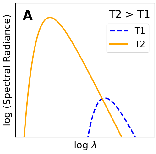
\includegraphics[width=0.48\linewidth]{2025_TH_T10-f1-panelA.pdf}\hfill
  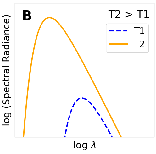
\includegraphics[width=0.48\linewidth]{2025_TH_T10-f1-panelB.pdf}\par\smallskip
  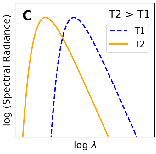
\includegraphics[width=0.48\linewidth]{2025_TH_T10-f1-panelC.pdf}\hfill
  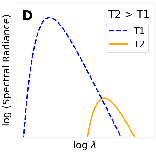
\includegraphics[width=0.48\linewidth]{2025_TH_T10-f1-panelD.pdf}\par\smallskip
  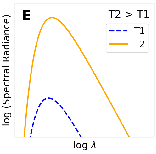
\includegraphics[width=0.48\linewidth]{2025_TH_T10-f1-panelE.pdf}
  \end{center}

\item[(T10.3)] After $t_{\mathrm{wk}}$, the process of formation of deuterium
  from protons and neutrons is governed by the Saha equation, given by the
  Indian physicist Prof.\ Meghnad Saha, which can be simplified to
  \[ \frac{N_{\mathrm{D}}}{N_{\mathrm{n}}}
     = 6.5\,\eta\left(\frac{k_B T}{m_{\mathrm{n}}c^2}\right)^{3/2}
       \exp\left(-\frac{(m_{\mathrm{D}} - m_{\mathrm{p}}
       - m_{\mathrm{n}})c^2}{k_B T}\right). \]
  Here, the baryon-to-photon ratio $\eta$ is $6.1 \times 10^{-10}$, and
  $N_{\mathrm{D}}$ is the number density of deuterium.
  \begin{description}
  \item[(T10.3a)] Plot the ratio $N_{\mathrm{D}}/N_{\mathrm{n}}$ on the grid
    in the Summary Answersheet, for at least 4 reasonably spaced values of
    temperature that lie in the domain $k_B T = [60, 70]$\,keV, and draw a
    smooth curve passing through these points. \hfill[5]
  \item[(T10.3b)] From the plot find $k_B T_{\mathrm{nuc}}$ (in keV) when
    $N_{\mathrm{D}} = N_{\mathrm{n}}$. \hfill[1]
  \item[(T10.3c)] Instead, now assume that all the free neutrons combine
    instantaneously with the protons at $k_B T_{\mathrm{nuc}}$ to form
    deuterium, all of which immediately gets converted to helium
    ($^4_2$He). Compute the corresponding epoch or time of nucleosynthesis,
    $t_{\mathrm{nuc}}$ (in s), for the formation of helium. \hfill[4]
  \end{description}
\item[(T10.4)] Calculate the value of $X_{\mathrm{n,nuc}}$ immediately before
  $t_{\mathrm{nuc}}$. \hfill[5]
\item[(T10.5)] The primordial helium abundance, $Y_{\mathrm{prim}}$, is
  defined to be the fraction of total mass in the Universe that is bound in
  helium at $T_{\mathrm{nuc}}$. Obtain a theoretical estimate for the value of
  $Y_{\mathrm{prim}}$. For the purpose of this calculation alone, assume
  $m_{\mathrm{p}} \approx m_{\mathrm{n}}$ and that the mass of helium,
  $m_{\mathrm{He}} \approx 4m_{\mathrm{n}}$. \hfill[3]
\item[(T10.6)] The primordial abundance of helium is very difficult to
  measure, as stars continuously convert hydrogen to helium in the Universe.
  The amount of processing by stars in a galaxy is characterised by the
  relative number density of oxygen (which is only produced by stars) to
  hydrogen, denoted as (O/H), in the galaxy. A compilation of the measurements
  of (O/H) and the helium abundance, $Y$, for different galaxies is plotted
  below. Use all of the points in this plot (which is reproduced in the
  Summary Answersheet) to answer the following.

  \ioaafig{2025_TH_T10-f2.pdf}

  \begin{description}
  \item[(T10.6a)] Estimate $Y$ for a blue compact dwarf galaxy with a value of
    $\mathrm{(O/H)} = 1.75 \times 10^{-4}$. \hfill[2]
  \item[(T10.6b)] Obtain the slope $dY/d\mathrm{(O/H)}$ of the straight line
    fit to the above data. \hfill[2]
  \item[(T10.6c)] Estimate the primordial helium abundance,
    $Y^{\mathrm{obs}}_{\mathrm{prim}}$, based on the above observations.
    \hfill[2]
  \end{description}
\item[(T10.7)] The deviation between $Y_{\mathrm{prim}}$ and
  $Y^{\mathrm{obs}}_{\mathrm{prim}}$ can be reconciled by changing the
  baryon-to-photon ratio $\eta$. When $\eta$ is decreased, as indicated by
  $\downarrow$ in the Summary Answersheet, indicate the increase ($\uparrow$)
  or decrease ($\downarrow$) in $N_{\mathrm{D}}/N_{\mathrm{n}}(T)$,
  $T_{\mathrm{nuc}}$ (when $N_{\mathrm{D}} = N_{\mathrm{n}}$),
  $t_{\mathrm{nuc}}$, $X_{\mathrm{n,nuc}}$, and $Y_{\mathrm{prim}}$ in the
  boxes provided in the Summary Answersheet. \hfill[3]
\end{description}

\section*{Data-analysis problems}

\probhead{13.24}{Virgo Cluster}{2008}{Bandung, Indonesia}{DA D1}{100}
% source id: 2008_DA_D1   tag: Virgo distance, H0, Hubble time
The Virgo cluster of galaxies is the nearest large cluster which extends over
nearly 10 degrees across the sky and contains a number of bright galaxies. It
is very interesting to find the distance to Virgo and to deduce certain
cosmological information from it. The table below provides the distance
estimates using various distance indicators (listed in the left column). The
right column lists the mean distance $d_i \pm$ the standard deviation $s_i$.

\begin{center}
\begin{tabular}{cl c}
$i$ & Distance Indicator & Virgo Distance (Mpc) \\
\hline
1 & Cepheids                       & $14.9 \pm 1.2$ \\
2 & Novae                          & $21.1 \pm 3.9$ \\
3 & Planetary Nebulae              & $15.2 \pm 1.1$ \\
4 & Globular Cluster               & $18.8 \pm 3.8$ \\
5 & Surface Brightness Fluctuation & $15.9 \pm 0.9$ \\
6 & Tully-Fisher relation          & $15.8 \pm 1.5$ \\
7 & Faber-Jackson relation         & $16.8 \pm 2.4$ \\
8 & Type Ia Supernovae             & $19.4 \pm 5.0$ \\
\end{tabular}
\end{center}

\begin{description}
\item[1.] By applying a weighted mean, compute the average distance (which can
  be taken as an estimate to the distance to Virgo)
  \[ d_{\mathrm{avg}}
     = \frac{\sum_i \dfrac{d_i}{s_i^2}}{\sum_i \dfrac{1}{s_i^2}} \]
  where the sum runs over the eight distance indicators used.
\item[2.] What is the uncertainty (rms) (in units of Mpc) in that estimate?
\item[3.] Spectra of the galaxies in Virgo indicate an average recession
  velocity of 1136\,km/sec for the cluster. Can you estimate the Hubble
  constant $H_0$ and its uncertainty (rms)?
\item[4.] What is the Hubble Time (age of the universe) using the value of the
  Hubble constant you found and the uncertainty (rms)?
\end{description}

\probhead{13.25}{The search for dark matter}{2017}{Phuket, Thailand}{DA D2}{75}
% source id: 2017_DA_D2   tag: LSB rotation curve, DM halo profile fit
A low surface brightness galaxy (LSB) is a diffuse galaxy with a surface
brightness that, when viewed from the Earth, is at least one magnitude lower
than the ambient night sky.

Some of its matter is in the form of ``baryonic'' matter such as neutral
hydrogen gas and stars. However, most of its matter is in the form of
invisible mass -- so called ``dark matter''. In this question, we will
investigate the mass of dark matter in a galaxy, the effect of dark matter on
the rotation curves of the galaxy, and the distribution of dark matter in the
galaxy.

The table below provides the data of a LSB galaxy named UGC4325. The galaxy is
assumed to be edge-on. At every distance $r$ from the centre of the galaxy, we
measure
\begin{enumerate}
\item $\lambda_{\mathrm{obs}}$, the observed wavelength of the H$\alpha$
  emission line. The Hubble expansion of the Universe has already been
  excluded from the data.
\item $V_{\mathrm{gas}}$, the contribution of the gas component to the
  rotation due to $M_{\mathrm{gas}}$, derived from HI surface densities.
\item $V_*$, the contribution of the stellar component to the rotation due to
  $M_*$, derived from R-band photometry.
\end{enumerate}
The rotational velocities of the test particle due to the gas component,
$V_{\mathrm{gas}}$, and the star component, $V_*$, are defined as the
velocities in the plane of the galaxy that would result from the corresponding
components without any external influences. These velocities are calculated
from the observed baryonic mass density distributions.

\begin{center}
\begin{tabular}{cccc}
$r$ & $\lambda_{\mathrm{obs}}$ & $V_{\mathrm{gas}}$ & $V_*$ \\
(kpc) & (nm) & (km/s) & (km/s) \\
\hline
 0.70 & 656.371 &  2.87 & 20.97 \\
 1.40 & 656.431 &  6.75 & 32.22 \\
 2.09 & 656.464 & 14.14 & 40.91 \\
 2.79 & 656.475 & 20.18 & 46.75 \\
 3.49 & 656.478 & 24.08 & 50.10 \\
 4.89 & 656.484 & 28.08 & 47.94 \\
 6.25 & 656.481 & 29.25 & 45.47 \\
 7.10 & 656.481 & 27.03 & 47.78 \\
 9.03 & 656.482 & 25.90 & 45.32 \\
12.05 & 656.482 & 21.03 & 42.30 \\
\end{tabular}
\end{center}

The mass of dark matter $M_{\mathrm{DM}}(r)$ within a volume of radius $r$ can
be defined in terms of the rotational velocity due to dark matter
$V_{\mathrm{DM}}$, the radius $r$ and the gravitational constant $G$,
\begin{equation}
M_{\mathrm{DM}}(r) = \frac{rV_{\mathrm{DM}}^2}{G}. \tag{1}
\end{equation}
To a good approximation, the observed rotational velocity $V_{\mathrm{obs}}$
can be modelled as
\begin{equation}
V_{\mathrm{obs}}^2 = V_{\mathrm{gas}}^2 + V_*^2 + V_{\mathrm{DM}}^2.
\tag{2}
\end{equation}
The observed rotational velocity $V_{\mathrm{obs}}$ depends on the mass of the
galaxy $M(r)$ within a volume of radius $r$ measured from the galaxy's centre.

The mass density $\rho_{\mathrm{DM}}(r)$ of dark matter within a volume of
radius $r$ can be modelled by a galaxy density profile,
\begin{equation}
\rho_{\mathrm{DM}}(r)
  = \frac{\rho_0}{1 + \left(\dfrac{r}{r_{\mathrm{C}}}\right)^2}
\tag{3}
\end{equation}
where $\rho_0$ and $r_{\mathrm{C}}$ are the central density and the core
radius of the galaxy, respectively. According to the density profile, the mass
of dark matter $M_{\mathrm{DM}}(r)$ within a volume of a radius $r$ can be
described by
\begin{equation}
M_{\mathrm{DM}}(r) = 4\pi\rho_0 r_{\mathrm{C}}^2
  \left[r - r_{\mathrm{C}}\arctan(r/r_{\mathrm{C}})\right].
\tag{4}
\end{equation}

\medskip
\textbf{Part 1 The mass of dark matter and rotation curves of the galaxy}

\begin{description}
\item[(D2.1)] In laboratories on Earth, H$\alpha$ has an emitted wavelength
  $\lambda_{\mathrm{emit}}$ of 656.281\,nm. Compute the observed rotational
  velocities of the galaxy $V_{\mathrm{obs}}$ and the rotational velocities
  due to the dark matter $V_{\mathrm{DM}}$ at distance $r$ in units of
  km\,s$^{-1}$.

  For the different values of $r$ given in the table, compute the dynamical
  mass $M(r)$ and the mass of dark matter $M_{\mathrm{DM}}(r)$ in solar
  masses. \hfill[21]
\item[(D2.2)] Create rotation curves of the galaxy on graph paper by plotting
  the points of $V_{\mathrm{obs}}$, $V_{\mathrm{DM}}$, $V_{\mathrm{gas}}$,
  $V_*$ versus the radius $r$ and draw smooth curves through the points (mark
  your graph as ``D2.2'').

  Order the contribution of the different components to the observed velocity
  in descending order. \hfill[16]
\end{description}

\medskip
\textbf{Part 2 Dark matter distribution}

\begin{description}
\item[(D2.3)] Take a data point at small $r$ and large $r$ to estimate
  $\rho_0$ and $r_{\mathrm{C}}$. Note that for large values of $x$,
  $\arctan(x) \approx \pi/2$ and at small $x$,
  $\arctan(x) \approx x - x^3/3$. \hfill[7]
\item[(D2.4)] By comparing Equation (4) to a linear function, the central
  density $\rho_0$ could also be found by a linear fit. Plot an appropriate
  graph so that a linear fit can be used to find another value of $\rho_0$.
  Evaluate $\rho_0$ in units of $M_\odot$\,kpc$^{-3}$. (Mark your graph as
  ``D2.4''). If you cannot find the value of $r_{\mathrm{C}}$ from the
  previous part, use $r_{\mathrm{C}} = 3.2$\,kpc as an estimate for this
  part. \hfill[19]
\item[(D2.5)] Compute logarithmic values of the dark matter density,
  $\ln[\rho_{\mathrm{DM}}(r)]$, and plot the distribution of dark matter in
  the galaxy as a function of radius $r$ on graph paper. (Mark your graph as
  ``D2.5''). \hfill[12]
\end{description}

\probhead{13.26}{Scaling Relations}{2021}{Bogot\'a (remote)}{DA DA1}{75}
% source id: 2021_DA_DA1   tag: Tully-Fisher fit, dark-to-baryonic masses
Spiral galaxies are disk-like rotating structures, whose dynamical state is
fairly grasped by the so-called rotation curves, quantifying the mean
rotational velocity of the disk at different distances from the center (see
Figure 1, curve B). An interesting feature is the flat region of the curve,
which is attributed to the presence of dark matter. Without it, rotation
velocities would drop steadily at large radii from the center, as depicted in
curve A.

\ioaafig[1.0]{2021_DA_DA1-f5.pdf}
% vs radius: curve A falling at large radii, curve B flattening (source paper
% Q1-1, "Figure 1: Rotation curves")

In disk galaxies a strong correlation has been observed between the intrinsic
luminosity of the whole galaxy and the asymptotic rotational velocity (as
given by the rotation curve for the outer edge of the galaxy, i.e.\
$R_{\max}$), a result that is known as the Tully--Fisher relation. This
relation also holds if you use the luminosity in a specific band. This is
shown on Figure 2 for a number of galaxies in a galaxy cluster. Every dot is a
galaxy, and the solid line is the best-fit linear relation between absolute
magnitude in $K$ band and $\log_{10}(V_{\max})$ for the whole sample.

\ioaafig{2021_DA_DA1-f1.pdf}

{\centering\small Figure 2: Absolute magnitude in $K$ band vs
$\log_{10}(V_{\max}\,[\mathrm{km\,s^{-1}}])$. Tully--Fisher relation for
several galaxies. Every dot represents a galaxy. The dark points are five
selected galaxies, for which we will provide some numbers in part 1.2.\par}

Another interesting trend is shown in Figure 3: disks with larger stellar
masses ($M_*$) tend to have smaller gas fractions ($M_{gas}/M_*$).

\ioaafig{2021_DA_DA1-f2.pdf}

In the following questions you will be asked to extract physical information
about the galaxies using the scaling relations just introduced. Consider the
following guidelines:
\begin{itemize}
\item Assume that $V_{\max}$ was measured at the same radius for all galaxies
  ($R_{\max}$), in the flat part of the rotation curves and well beyond the
  end of the stellar disk.
\item Use $M_{dm}$ for the dark matter mass up to $R_{\max}$ and $M_{tot}$
  for the sum of all components (gas, stars and dark matter).
\item Assume that all galaxies have identical stellar populations (the term
  stellar population refers to the type of stars that are present in a
  galaxy, and the relative amount of each type with respect to the total
  number of stars), and assume that the gaseous component does not interact
  with the stellar light.
\item The galaxy cluster is far away. Its distance is much larger than the
  cluster size.
\item In spherically-symmetric mass distributions, to infer the gravitational
  effect on a particle at distance $r$ from the center, it suffices to
  consider the total mass enclosed up to that radius $M(\leq r)$ as if it
  were placed at the very center of the distribution.
\end{itemize}

\medskip
\textbf{Part 1 (20 points).}

\begin{description}
\item[1.1] From an analysis of Figure 3, find the appropriate constants in the
  following relation: $M_{gas} = a \times M_*^b$
  \[ a = ?\qquad b = ? \]
  \hfill[5.0\,pt]
\item[1.2] In the plot of the Tully--Fisher relation there are 5 highlighted
  points. Data for these 5 galaxies is given in the following table. Use this
  dataset to find the appropriate constants for the TF relation presented
  below the table, by means of a linear fit using the method of least
  squares.

  \emph{Note:} Treat $\log_{10}(V_{\max})$ as the $x$ variable and $K$ as the
  $y$ variable in the linear fit.

  \begin{center}
  \begin{tabular}{cc}
  $V_{\max}$ [km/s] & $K$ [mag] \\
  \hline
   79.4 & $-16.8$ \\
  100.1 & $-19.2$ \\
  158.5 & $-21.3$ \\
  251.2 & $-21.4$ \\
  316.2 & $-24.0$ \\
  \end{tabular}
  \end{center}

  \[ K = c \times \log_{10}(V_{\max}) + d \]
  \[ c = ?\qquad d = ? \]
  \hfill[15.0\,pt]
\end{description}

\medskip
\textbf{Part 2 (16 points).}

For two galaxies, G1 and G2, in the cluster, the recorded \emph{apparent}
magnitudes are:
\[ k_1 = 19.2\,;\qquad k_2 = 25.2 \]
Using this information and the relations calibrated in Part 1, find the
correct exponents in the following equations:

\begin{description}
\item[2.1] $\dfrac{M_{*1}}{M_{*2}} = 10^e$;\quad $e = ?$ \hfill[6.0\,pt]
\item[2.2] $\dfrac{M_{gas1}}{M_{gas2}} = 10^f$;\quad $f = ?$ \hfill[4.0\,pt]
\item[2.3] $\dfrac{M_{tot1}}{M_{tot2}} = 10^g$;\quad $g = ?$ \hfill[6.0\,pt]
\end{description}

\medskip
\textbf{Part 3 (15 points).}

\begin{description}
\item[3.1] Fill in the missing values in the table using the fact that for
  galaxy $G_1$, the dark-to-baryonic mass ratio up to $R_{\max}$ is 6.82.
  \hfill[15.0\,pt]

  \begin{center}
  \begin{tabular}{cccccc}
  Galaxy & Apparent magnitude $k$ & $M_{gas}\,[M_\odot]$ & $M_*\,[M_\odot]$ &
  $M_{dm}\,[M_\odot]$ & $M_{tot}\,[M_\odot]$ \\
  \hline
  $G_1$ & 19.2 & & & & $4.39 \times 10^{11}$ \\
  \end{tabular}
  \end{center}
\end{description}

\medskip
\textbf{Part 4 (24 points).}

\begin{description}
\item[4.1] Consider a systematic uncertainty of $\sigma_{sys} = \pm 0.2$ in
  each apparent magnitude due to CCD calibration errors. Then $k_1$ must be
  read as $k_1 = 19.2 \pm 0.2$, i.e., the only thing we know is that $k_1$
  most likely lies in the interval $[19.0, 19.4]$. The same goes for $k_2$.

  Recalculate the exponent in the scaling relation
  $\frac{M_{*1}}{M_{*2}} = 10^e$ (found in 2.1), expressing $e$ as an
  interval estimated by considering the extreme possible variations in $k_1$
  and $k_2$.
  \[ e \in [?, ?] \]
  \hfill[4.0\,pt]
\item[4.2] Now we consider that there is always a natural spread of the data
  around any relation. For instance, for a given value of the $K$ magnitude
  the TF relation gives a single value of $\log_{10}(V_{\max})$, but it would
  be more realistic to report an interval of plausible values, derived from
  the natural spread of the data around the mean TF relation. We call this
  the statistical uncertainty, $\sigma_{stat}$.

  Estimate the statistical uncertainty if $\log_{10}(V_{\max})$ is inferred
  from $K$ using the TF relation from question 1.2. For this, consider for
  each point the difference between the value of $\log_{10}(V_{\max})$
  estimated from $K$ using your linear fit and the actual measurement of
  $\log_{10}(V_{\max})$, and take $\sigma_{stat}$ as two times the root mean
  square (RMS) of these differences (the RMS of a set of values is the square
  root of the arithmetic mean of the squares of those values).
  \[ \sigma_{stat} = ? \]
  \hfill[10.0\,pt]
\item[4.3] Recalculate the exponent in the scaling relation
  $\frac{M_{tot1}}{M_{tot2}} = 10^g$, expressing $g$ as an interval estimated
  by considering the extreme possible variations arising from both the
  systematic and statistical uncertainties:
  \[ g \in [?, ?] \]
  \hfill[10.0\,pt]
\end{description}

\probhead{13.27}{Galactic Surveys}{2022}{Kutaisi, Georgia}{DA 2}{105}
% source id: 2022_DA_2   tag: halo pair statistics, redshift-space distortions
In Cosmology, observations of the spatial distribution of galaxies are crucial
to understanding the evolution and expansion of the Universe. Numerous
telescopes conduct surveys to produce catalogues of galaxies, which are then
subjected to statistical analysis. Usually, galaxies form in groups, which
together are part of a cluster, surrounded by a very large, spherical
dark-matter halo. Most of the matter is concentrated in the centre, thus there
is a high probability of having a large-mass galaxy at the centre of the halo.

In this problem, we will assume that all halos have one central galaxy and
several groups of satellite galaxies, and use statistical analysis to draw
inferences about the spatial distribution of galaxies. In Figure 1, you can
see six different possible probability densities (A--F) for distances between
galaxies. On the X axis is the separation distance between galaxies ($a$), and
on the Y axis is the probability density ($f_p(a)$). The probability of the
distance between a pair of galaxies being in the range $a$ to $a + \Delta a$
is given by
\[ P(a) = f_p(a)\,\Delta a \]
Note that $f_p(a)$ may take values greater than 1 in some cases.

\ioaafig{2022_DA_2-f5.pdf}
% densities f_p(a) vs separation a (source paper, Data Analysis page 3 of 7,
% "Figure 1: Probability density of all possible galaxy pairs")

\medskip
\textbf{Part 1 (60\,pt)}

Table 1 gives the observational data of a single dark matter halo in the form
of Cartesian coordinates of 16 satellite groups and the coordinates of the
central galaxy, which is given in the first row. The $i^{\mathrm{th}}$ group
consists of $N_i$ galaxies. The origin of this coordinate system is the Earth.
For simplicity we assume that a group of galaxies means a collection of
galaxies with almost the same coordinates.

\begin{center}
\begin{tabular}{ccccc}
$i$ & $x$ (Mpc) & $y$ (Mpc) & $z$ (Mpc) & $N_i$ \\
\hline
C  & 8.300 & 6.200 &  1.100 & Central \\
\hline
1  & 8.401 & 6.309 &  1.394 & 291 \\
2  & 9.883 & 7.189 &  1.506 & 170 \\
3  & 8.883 & 6.413 &  2.226 & 253 \\
4  & 8.444 & 6.569 &  2.439 & 8   \\
5  & 7.782 & 6.048 & $-0.358$ & 72  \\
6  & 8.780 & 6.305 &  2.463 & 120 \\
7  & 7.990 & 5.881 &  0.532 & 302 \\
8  & 8.540 & 6.388 &  0.369 & 52  \\
9  & 7.975 & 6.030 &  1.216 & 28  \\
10 & 7.072 & 5.431 &  0.488 & 40  \\
11 & 8.037 & 5.965 &  0.615 & 72  \\
12 & 8.681 & 6.483 &  0.734 & 379 \\
13 & 7.115 & 5.259 &  1.403 & 82  \\
14 & 9.587 & 7.130 &  0.322 & 62  \\
15 & 8.193 & 6.104 &  0.915 & 305 \\
16 & 7.613 & 5.847 &  1.666 & 293 \\
\end{tabular}
\end{center}

\begin{description}
\item[(a)] The distribution of the satellite groups in the $X-Z$ plane and
  $Y-Z$ plane has been plotted for you. Plot the distribution in the $X-Y$
  plane on millimeter paper. \hfill(6\,pt)

  \ioaafig{2022_DA_2-f2.pdf}

\item[(b)] Given that this cluster of galaxies is shaped like a disk and our
  line of sight is in the plane of the disk, find the unit vector in the
  direction of the normal to the disk. \hfill(4\,pt)
\item[(c)] Let us define a new coordinate system centered on the central
  galaxy, defining our line of sight from the Earth to the central galaxy as
  the $X'$ axis and the normal to the disk as the $Z'$ axis. Find the unit
  vectors for this coordinate system. \hfill(2\,pt)
\item[(d)] Convert the given Cartesian coordinates to the new $X'Y'Z'$
  coordinates. Calculate $X'$, $Y'$, $Z'$. \hfill(24\,pt)
\item[(e)] Write the equations necessary to convert the new $X'Y'Z'$
  Cartesian coordinates into spherical coordinates centered on the central
  galaxy. The $\theta$ coordinate has been already calculated for you below.
  Calculate $R$ and $\phi$. \hfill(11\,pt)

  \begin{center}
  \begin{tabular}{cc}
  $i$ & $\theta$ \\
  \hline
  1  & 1.652 \\
  2  & 1.490 \\
  3  & 1.432 \\
  4  & 1.721 \\
  5  & 1.692 \\
  6  & 1.430 \\
  7  & 1.474 \\
  8  & 1.580 \\
  9  & 1.723 \\
  10 & 1.646 \\
  11 & 1.519 \\
  12 & 1.569 \\
  13 & 1.542 \\
  14 & 1.557 \\
  15 & 1.516 \\
  16 & 1.705 \\
  \end{tabular}
  \end{center}

  \emph{Note:} in spherical coordinates, one uses the coordinates $R$,
  $\theta$ and $\phi$, where $R$ is the radial distance, $\phi$ is the
  azimuthal angle measured anti-clockwise from the $X'$ axis (from 0 to
  $2\pi$) and $\theta$ is the polar angle (from 0 to $\pi$), i.e.\ the angle
  relative to the $Z'$ axis.
\item[(f)] Plot a histogram (on millimeter paper) showing the number of
  satellite galaxies at different radial distances from the central galaxy.
  Use 8 equally sized bins for radial distances, with 0.2\,Mpc to 2\,Mpc as
  the total range of the histogram. \hfill(9\,pt)
\item[(g)] The histogram must also be converted into a probability density. On
  the right hand side of the vertical axis of the histogram you plotted, add
  markings for the re-scaled vertical axis appropriate for the probability
  density. You will use this probability density data in part 3. \hfill(4\,pt)
\end{description}

\medskip
\textbf{Part 2 (17\,pt)}

The coordinates in the Table above are determined using distances obtained by
the redshift method. It is well-known that while measuring distance to any
galaxy with the redshift method, errors might occur because of the orbital
motion of the galaxies. Now, we will try to correct for these errors. Assume
that the central galaxy has an effective mass of $1 \times 10^{10}\,M_\odot$,
all satellite galaxies move in circular orbits around the central galaxy and
interactions between any two satellite galaxies can be ignored.

\begin{description}
\item[(a)] Use the data in Table 1 of the question sheet to obtain a histogram
  of number of galaxies against the $\phi$ azimuthal angle (take the width of
  the bins as $60^\circ$). The angle distribution is expected to be uniform,
  but it is not. Calculate the standard deviation for this data. \hfill(5\,pt)
\item[(b)] The two bins centered along the $Y'$ axis show an unusually low
  number of galaxies as the orbital velocities of satellite galaxies in these
  bins are almost parallel to our line of sight and hence there is maximum
  error in their distance estimated by the redshift method. Derive an
  expression for the correction in each azimuthal angle. \hfill(4\,pt)

  \emph{Note:} You may assume that the distance from the central galaxy ($R$)
  doesn't change significantly because of this correction.
\item[(c)] Calculate the corrected value of the azimuthal angles for each data
  row and recalculate the histogram and its standard deviation of its values.
  \hfill(8\,pt)
\end{description}

\medskip
\textbf{Part 3 (28\,pt)}

So far, we have only calculated the central galaxy -- satellite galaxy
histogram for a single halo. It is time to move on to calculating other
relations. The same observations and data analysis has been carried out for
different halos and their central galaxies. Suppose we have 500 halos, thus,
500 central galaxies ($N_C = 500$). Take that the average number of satellite
galaxies in each halo is 1000 ($N_S = 1000$).

\begin{description}
\item[a)] Calculate the following quantities:
  \begin{description}
  \item[(1)] $N_{CC}$, total number of pairs of central galaxies.
  \item[(2)] $N_{CS}^*$, total number of central galaxy -- satellite pairs
    such that the galaxies in the pair belong to the same halo.
  \item[(3)] $N_{CS}$, total number of central galaxy -- satellite pairs such
    that the galaxies in the pair belong to two separate halos.
  \item[(4)] $N_{SS}^*$, total number of satellite -- satellite galaxy pairs
    such that the galaxies in the pair belong to the same halo.
  \item[(5)] $N_{SS}$, total number of satellite -- satellite galaxy pairs
    such that the galaxies in the pair belong to two separate halos.
  \end{description}

  The table below gives the probability density values for different distances
  between central galaxies in different dark matter halos (CC). You should
  note this data is not real and doesn't represent the results of the real
  observations. Dark matter halos do not intersect. But for simplicity we will
  use this data.

  \begin{center}
  \begin{tabular}{cc}
  $R$ (Mpc) & $\rho_{CC}$ \\
  \hline
  0.3125 & 0.406 \\
  0.5375 & 0.808 \\
  0.7625 & 1.341 \\
  0.9875 & 1.134 \\
  1.2125 & 0.479 \\
  1.4375 & 0.143 \\
  1.6625 & 0.073 \\
  1.8875 & 0.060 \\
  \end{tabular}
  \end{center}

  We can calculate all probability densities using the given Center-Center
  (CC) data and the same halo Center-Satellite ($CS^*$) data that we have
  calculated in part 1. We use the following relations:
  \[ \rho_{SS}^*(R) = c_1 R\left(\rho_{CS}^*(R)\right)^2 \]
  \[ \rho_{CS}(R) = c_2 R\left(\rho_{CS}^*(R)\right)^2
     \sqrt{\rho_{CC}(R) + 1} \]
  \[ \rho_{SS}(R) = c_3 R\left(\rho_{CS}^*(R)\left(\rho_{CC}(R)
     - 5\right)\right)^2 \]
  where $c_1$, $c_2$ and $c_3$ are normalization constants and should be found
  for each probability density.
\item[b)] Calculate normalized $\rho_{SS}^*(R)$, $\rho_{CS}(R)$,
  $\rho_{SS}(R)$. \hfill(15\,pt)
\item[c)] Calculate the final probability density of all galaxy pairs, that
  combines all the distributions above with appropriate weights. Which one of
  the 6 graphs on Fig.~1 best represents this probability density?
  \hfill(8\,pt)
\end{description}

\clearpage
\section*{Solutions to Chapter 13}

\solhead{13.1}{}
% source id: 2008_TH_L3
\ioaafig{2008_TH_L3-s1.pdf}

\begin{description}
\item[a)] $X_0 = d\theta_0$, where $d = c(t_o - t_r) \approx ct_o$,
$t_o \gg t_r$.

Scale factor $S$ is defined as such $S_0 = S(t=t_o) = 1$ and
$S_t = S(t<t_o) < 1$. Maximum distance between objects at the time of
recombination
\[
X_r = S_r X_o = S_r \theta_o t_o c
\]
On the other hand $X_r = ct_r$, such that
\[
ct_r = S_r\theta_0 t_o c
\qquad\text{or}\qquad
\theta_o = \frac{t_r}{S_r t_o}
\]
\hfill(20\%)

From $T \propto \dfrac{1}{S}$ then
$\dfrac{S_o}{S_r} = \dfrac{T_r}{T_o}$ and
$\dfrac{1}{S_r} = \dfrac{T_r}{T_o}$.

So,
\[
\theta_o = \frac{t_r T_r}{t_o T_o}
= \frac{(3\times10^{5}\ yr)(3000\ K)}{(1.5\times10^{10}\ yr)(3\ K)}
= 2\times10^{-2}\ rad = 1.14^\circ
\]
\hfill(20\%)

\item[b)] NO, because $\alpha > \theta_o$
\hfill(20\%)

\item[c)]
\ioaafig{2008_TH_L3-s2.pdf}
From the time at recombination ($t_r$) to the current time ($t_0$)
$S \propto t^{2/3}$, we derive
\[
\frac{S_o}{S_r} = \left(\frac{t_o}{t_r}\right)^{2/3}
= \left(\frac{1.5\times10^{10}\ years}{3\times10^{5}\ years}\right)^{2/3}
= 1.36\times10^{3}
\]
The size of our universe at $t_r$ is
\[
\frac{1.5\times10^{10}\ \text{light years}}{1.36\times10^{3}}
= 1.11\times10^{7}\ \text{light years}
\]
\hfill(20\%)

When the inflation stopped, the Universe was radiation dominated
($t_r = 3\times10^{5}$ years to $t_i = 10^{-32}$ s), we get
\[
\frac{S_r}{S_i} = \left(\frac{t_r}{t_i}\right)^{1/2}
= \left(\frac{9.46\times10^{12}\ s}{10^{-32}\ s}\right)^{1/2}
= 3.08\times10^{22}.
\]
The size of universe at the end of the inflation period was
\[
\frac{1.1\times10^{7}\ \text{light years}}{3.08\times10^{22}}
= 3.57\times10^{-16}\ \text{light years} \approx 3\ m
\]
\hfill(20\%)
\end{description}

\solhead{13.2}{}
% source id: 2008_TH_S12
The relation between flux $F$ and luminosity $L$:
$F = \dfrac{L}{4\pi d^2}$.

For Vega:
\[
F_V = \frac{L_V}{4\pi\,d_V^2}
\]
For Supernova:
\[
F_{SN} = \frac{L_{SN}}{4\pi\,d_{SN}^2}
\]
\begin{align*}
F_{SN} = 1.6\times10^{-7}F_V
\quad\Longrightarrow\quad
\frac{L_{SN}}{4\pi\,d_{SN}^2}
  &= \left(1.6\times10^{-7}\right)\frac{L_V}{4\pi\,d_V^2}\\
L_{SN}\,d_V^2 &= \left(1.6\times10^{-7}\right)L_V\,d_{SN}^2
\end{align*}
\hfill(25\%)
\begin{align*}
d_{SN} &= d_V\left[\frac{1}{1.6\times10^{-7}}\,
  \frac{L_{SN}}{L_V}\right]^{1/2}
= 7.76\left[\frac{1}{1.6\times10^{-7}}\,
  \frac{5.8\times10^{9}}{130}\right]^{1/2}
= 129\,581\,812.59\ \mathrm{pc}\\
&= 1.3\times10^{8}\ \mathrm{pc}
\end{align*}
\hfill(35\%)

If $t_H$ is the Hubble time, then the relation between redshift, distance, and
Hubble time is:
\[
t_H = \frac{d_{SN}}{cz}
= \left[\frac{1.3\times10^{8}\ \mathrm{pc}}
  {(1\ \mathrm{lyr/yr})(0.03)}\right]
  \left(\frac{3.26\ \mathrm{lyr}}{1\ \mathrm{pc}}\right)
= 1.41\times10^{10}\ \mathrm{years}
\]
\hfill(40\%)

\solhead{13.3}{}
% source id: 2008_TH_S5
Universe change in size and redshift relation:
\[
1+z = \frac{\mathrm{size}_{\mathrm{now}}}{\mathrm{size}_{\mathrm{at}\,z}}
\quad\Longrightarrow\quad
\mathrm{size}_{\mathrm{at}\,z} = \frac{1}{1+z}\,\mathrm{size}_{\mathrm{now}}
= \frac{1}{1+1100}\,\mathrm{size}_{\mathrm{now}}
= 0.00091\,\mathrm{size}_{\mathrm{now}}
\]
so that the size of the Universe at the time of CMB emission was $0.00091$ of
its $\mathrm{size}_{\mathrm{now}}$.
\hfill(50\%)

If
\[
A = \frac{V_{\mathrm{CMB\ at\ emission\ time}}}{V_{\mathrm{Now}}}
= (0.00091)^3 = 7.5\times10^{-10},
\]
then the density of the Dark Matter at CMB emission time
\[
\rho_{\mathrm{DM\ at\ CMB}} = \frac{\rho_{\mathrm{DM}}}{A}
= \frac{2.4\times10^{-30}}{7.5\times10^{-10}}
= 3.2\times10^{-21}\ \mathrm{g/cm^3}.
\]
\hfill(25\%)

The ratio between the density of Dark Matter to the density of Dark Energy at
the time CMB was emitted
\[
= \frac{\rho_{\mathrm{DM\ at\ CMB}}}{\rho_{\Lambda}}
= \frac{3.2\times10^{-21}}{6.7\times10^{-30}} = 4.8\times10^{8}
\]
\hfill(25\%)

\solhead{13.4}{}
% source id: 2009_TH_P11
In a flat universe
\begin{equation*}
\rho = \rho_c = \frac{3H^2}{8\pi G} \tag*{(4 points)}
\end{equation*}
\begin{equation*}
H = 75~\mathrm{km\,s^{-1}\,Mpc^{-1}} = 2.4\times10^{-18}~\mathrm{s^{-1}}
\tag*{(2 points)}
\end{equation*}
\begin{equation*}
\rho_c = 1.1\times10^{-26}~\mathrm{kg\,m^{-3}} \tag*{(2 points)}
\end{equation*}
\begin{equation*}
n_\nu = \frac{0.25\,\rho_c}{10^{-5}\,m_e} = 3\times10^{8}~\mathrm{m^{-3}}
\tag*{(2 points)}
\end{equation*}

\solhead{13.5}{}
% source id: 2010_TH_S3
Recession velocity of the QSO is
\begin{equation*}
\frac{v}{c} = \frac{(z+1)^2 - 1}{(z+1)^2 + 1} = 0.18 \tag*{4}
\end{equation*}
According to the Hubble's law,
\begin{equation*}
v = H_0 D \tag*{2}
\end{equation*}
The distance of the QSO is
\begin{equation*}
D = v/H_0 = 0.18c/72 = 750~\mathrm{Mpc}, \tag*{4}
\end{equation*}

Remarks: if the student calculate the distance using cosmological formula and
arrive at the answer $D = 735~\mathrm{Mpc}$, assuming $\Omega_0 = 1.0$ will
get the full mark.

\solhead{13.6}{}
% source id: 2011_TH_S11
Within assumed cosmological model the following relation is valid:
\[
(1+z) = \frac{R_0}{R(z)} = \left(\frac{t_0}{t(z)}\right)^{2/3},
\]
where $R_0$ and $R(z)$ denote the current value of the scale factor and that
for the redshift equal to $z$ respectively, while $t_0$ and $t(z)$ stands for
the time that passed from the Big Bang. \hfill[5]

For $z=6.03$ the appropriate time $t(z) = 7.35\cdot10^{8}$ years. Subtracting
from $t(z)$ the interval equal to 560 My and 600 My one obtains
$t_1 = 1.75\cdot10^{8}$\,y and $t_2 = 1.35\cdot10^{8}$\,y \hfill[3]

what is equivalent to $z_1 = 17.3$ and $z_2 = 20.8$. \hfill[2]

\solhead{13.7}{}
% source id: 2011_TH_S15
Correct choice of the wavelength: \hfill[2]

If the nature of the spectrum does not change, it is sufficient to perform the
calculation for one wavelength. The simplest choice is for the wavelength of
the maximum (Wien's law)
\[
\lambda = b/T
\]

Understanding definition of redshift \hfill[2]

From this
\[
z = (\lambda_a - \lambda_e)/\lambda_e
\]
where $\lambda_a$ is the wavelength received at the Earth and $\lambda_e$ is
the emitted wavelength, thus $\lambda_e = \lambda_a/(z+1)$.

Substituting into Wien's law, we find
\[
T = b\cdot(z+1)/\lambda_a
\]
\hfill[4]

Substituting the current value of the temperature we find the result \hfill[2]

\solhead{13.8}{}
% source id: 2012_TH_S10
As we have a differential equation that should be integrated, we expect that
the student can solve it in two ways: using an approximation (Way 1) or
calculus (Way 2). \hfill(2 pt finding final scale factor)

\medskip
\noindent\textit{Way 1.}
Using the definition of Hubble constant:
$\dfrac{da}{dt} = Ha$, where $a$ is the scale factor and using the
approximation $\dfrac{da}{dt} \approx \dfrac{\Delta a}{\Delta t}$, and
supposing that the variation of the scale factor and the Hubble constant is
small compared to their values, and using that $aT = \mathrm{const}$:
\begin{equation*}
\frac{\Delta a}{\Delta t} = H_i a_i
\;\Rightarrow\;
\frac{\Delta T}{\Delta t} = -H_i T_i
\;\Rightarrow\;
\Delta t = -\frac{1}{H_i}\,\frac{\Delta T}{T_i} = 5.0\cdot10^{8}~years
\tag*{(7 pt + 1 pt)}
\end{equation*}

\medskip
\noindent\textit{Way 2.}
As we have a matter dominated Universe ($\rho \propto a^{-3}$), without dark
energy, and a density parameter $\Omega_0 = 1$, we have:
\begin{equation*}
\Omega_0 = \frac{8\pi G\rho}{3H^2} = \frac{8\pi G}{3H^2}\,\frac{\zeta}{a^3} = 1
\tag*{(4 pt)}
\end{equation*}
From the Hubble law, $\dfrac{da}{dt} = Ha$:
\[
\left(\frac{da}{dt}\right)^{2} = \frac{8\pi G}{3}\,\frac{\zeta}{a}
\;\Rightarrow\;
\frac{da}{dt} = \sqrt{\frac{8\pi G}{3}\,\frac{\zeta}{a}}
\]
Integrating this equation: \hfill(3 pt)
\[
\frac{2}{3}\left[a_f^{3/2} - a_i^{3/2}\right]
= \sqrt{\frac{8\pi G}{3}\,\zeta}\,\Delta t
\;\Rightarrow\;
\Delta t
= \frac{2}{3}\left[\left(\frac{a_f}{a_i}\right)^{3/2} - 1\right]
  \frac{1}{\sqrt{\dfrac{8\pi G}{3}\,\dfrac{\zeta}{a_i^{3}}}}
= \frac{2}{3}\,\frac{1}{H_i}
  \left[\left(\frac{a_f}{a_i}\right)^{3/2} - 1\right]
\]
Using the fact that $aT = \mathrm{const}$:
\[
a_i T_i = a_f T_f
\;\Rightarrow\;
\frac{a_f}{a_i} = \frac{T_i}{T_f} = \frac{2.73}{2.63} = 1.038
\]
So the time is:
\begin{equation*}
\Delta t = 5.2\cdot10^{8}~years \tag*{(1 pt)}
\end{equation*}
Obs: (7 pt for using correctly that $a \propto t^{2/3}$)

\solhead{13.9}{}
% source id: 2013_TH_L1
\begin{description}
\item[(1)] The critical density $\rho_c = \dfrac{3H_0^2}{8\pi G}$
\hfill(9 points)

If the matter density parameter
$\Omega_m = \dfrac{\rho_m}{\rho_c}$ is 32\%, thus
$\rho_m = 0.32\,\dfrac{3H_0^2}{8\pi G}$.
\hfill(3 points)

From the latest estimate of
$H_0 = 67.8\ \dfrac{\mathrm{km\,s^{-1}}}{Mpc}$ we obtain
$\rho_m = 8.6\times10^{-27}$ kg m$^{-3}$
% sic: 8.6e-27 kg/m^3 is the critical density for H_0 = 67.8; the matter
% density with the 0.32 factor would be 2.8e-27 kg/m^3.
\hfill(4 points)

\item[(2)] The escape velocity is
$\upsilon_{esc} = \sqrt{\dfrac{2GM}{d}}$.
\hfill(4 points)

By replacing $M = \rho_c\,\dfrac{4\pi}{3}d^3$
\hfill(2 points)

we obtain, for the escape velocity within $d = 100$ Mpc
\[
\upsilon_{esc}
= \sqrt{\frac{8\pi}{3}G\times0.32\times\frac{3H_0^2}{8\pi G}}
  \times 100\,Mpc
= 3835\ \mathrm{km\,s^{-1}}
\]
\hfill(8 points)

\item[(3)] If a galaxy is orbiting around the centre of our galaxy, its
velocity is $\dfrac{1}{\sqrt{2}}$ of its escape velocity. Thus
\[
\omega = \frac{v}{d} = \frac{v_{esc}/\sqrt{2}}{d}
= \frac{H_0 d\sqrt{\Omega_m/2}}{d}
= \frac{\sqrt{0.32}\,(67.8\times10^{3}\,m/s)/(3.09\times10^{22}\,m)}
  {\sqrt{2}}
= 8.8\times10^{-19}\ rad/s
\]
\hfill(12 Points)

This is $1.8\times10^{-13}\ arc\sec/s$ and it does not depend on the
distance $d$.

\item[(4)] Therefore we will never be able to resolve them and the answer is
``No''.
\hfill(8 Points)
\end{description}

\solhead{13.10}{}
% source id: 2013_TH_L3
\begin{description}
\item[(1)] Using the virial theorem for our isolated, spherical system of $N$
galaxies of mass $m$, each, we get
\[
-2\langle K\rangle = \langle U\rangle
\;\Rightarrow\;
-\frac{2}{N}\sum_{1}^{N}\frac{1}{2}m_i u_i^2 = \;<U>
\;\Rightarrow\;
-\frac{m}{N}\sum_{1}^{N}u_i^2 = \frac{U}{N}
\]
\hfill(3 point)

where
$\dfrac{1}{N}\displaystyle\sum_{1}^{N}u_i^2 \approx \langle u^2\rangle
= \langle u_r^{\,2}\rangle + \langle u_\theta^{\,2}\rangle
+ \langle u_\phi^{\,2}\rangle$,
where $u_r$, $u_\theta$ and $u_\phi$ are the radial velocity and the two
perpendicular velocities on the plane of the sky of the members of the
cluster.
\hfill(6 points)

Assuming that
$\langle u_r^{\,2}\rangle \sim \langle u_\theta^{\,2}\rangle
\sim \langle u_\phi^{\,2}\rangle$, we have
\[
-3m\langle u_r^2\rangle = U/N
= \Bigl(-\frac{3}{5}\frac{GM^2}{R}\Bigr)/N
= -\frac{3}{5}\frac{GMm}{R}
\;\Rightarrow\;
M \approx \frac{5R\langle u_r^2\rangle}{G}
\]
\hfill(13 points)

(where we used the gravitational potential of a spherical homogeneous mass
$M$ enclosed within radius $R$)

Alternatively the student can give a rougher order of magnitude estimate
\[
-2\langle K\rangle = \langle U\rangle
\;\Rightarrow\;
-2.\frac{1}{2}\langle u_r^2\rangle \approx -\frac{GM}{R}
\quad\text{etc}
\]
If they do not use the exact formula:
\hfill(11 Points)

\item[(2)] From the result of the previous question we have
$M \approx \dfrac{5R\langle u_r^2\rangle}{G}$, where
\[
\sqrt{\langle u_r^2\rangle} = \sigma = 1000\ km\,s^{-1}
\]
\hfill(8 points)

The angular diameter of the cluster is $\varphi = 4^\circ$ at a distance of
$d = 90$ Mpc. Therefore the diameter D of the cluster in Mpc is calculated
from:
\[
\tan\phi = \frac{D}{d}
\;\Rightarrow\;
\phi(rad) \approx \frac{D}{d}
\;\Rightarrow\;
D \approx 4\times\frac{\pi}{180}\times90\,\mathrm{Mpc} \approx 6.3\,Mpc
\;\Rightarrow\;
R \approx 3\,Mpc
\]
\hfill(11 points)

Therefore
$M \approx \dfrac{5R\langle u_r^2\rangle}{G} = 3.6\times10^{15}\,\mathrm{M}_\odot$
\hfill(3 point)

\item[(3)]
\[
\frac{M_{virial}}{L_{galaxies}}
= \frac{3.6\times10^{15}\,\mathrm{M}_\odot}{5\times10^{12}\,L_\odot}
= 720\,\frac{\mathrm{M}_\odot}{L_\odot}
\]
This is obviously much larger from
$\dfrac{\mathrm{M}_\odot}{L_\odot} = 1$ which is found from the visible mass
of the cluster. Thus $\dfrac{M}{M_{virial}} = \dfrac{1}{720}$.
\hfill(6 points)
\end{description}

\solhead{13.11}{}
% source id: 2013_TH_S15
The recession velocity is calculated by either the classical relation,
$v_c = z\times c$, or the relativistic relation,
\[
v_r = \frac{(1+z)^2 - 1}{(1+z)^2 + 1}\,c.
\]
The calculations for the three galaxies are summarized in the following
Table:

\begin{center}
\begin{tabular}{|c|c|c|c|c|}
\hline
Galaxy & $v_c$ (km/s) & $V_a$ (km/s) & $v_r$ (km/s) & $v_r/c \times 100$\\
\hline
3C279 & 160800 & 128750 & 121390 & 40\%\\
\hline
3C245 & 308700 & 212260 & 182740 & 61\%\\
\hline
4C41.17 & 1140000 & 470580 & 275040 & 92\%\\
\hline
\end{tabular}
\end{center}

\begin{description}
\item[(1)] Table 1, Columns 2,3,4 \hfill(5 Points)
\item[(2)] Column 5 \hfill(3 Points)
\item[(3)] If the student answers ``Classical'' \hfill(0 Points)\\
  If the student answers ``Special Relativity'' \hfill(1 Point)\\
  If the student answers ``Approximate formula'' \hfill(2 Points)
\end{description}

\solhead{13.12}{}
% source id: 2013_TH_S5
\begin{description}
\item[(a)]
\[
z = \frac{\lambda - \lambda_o}{\lambda_o}
= \frac{662.9 - 656.3}{656.3} \approx 0.01.
\]
\hfill(3 Point)

This is small enough that we can use the classical equation for the expansion
of the Universe.
\[
H_o = \frac{cz}{r}
= \frac{3\times10^{5}\ \mathrm{km\,s^{-1}} \times 10^{-2}}{41.67\ Mpc}
\quad\text{or}\quad
H_o = 72.4\ \frac{\mathrm{km\,s^{-1}}}{Mpc}
\]
\hfill(4 Points)

\item[(b)] $t_H \approx \dfrac{1}{H_o}$ or $t_H = 13.5$\,\textbf{Gyr}
\hfill(3 Point)
\end{description}

\solhead{13.13}{}
% source id: 2015_TH_S14
To decide how far one can see on average in a universe filled with spherical
objects of radius $R$, it is simplest to think of a long cylinder along the
line of sight. If an object is closer than $R$ to the line of sight, then the
line of sight intersects its surface. For a distance $\ell$, the cylindrical
volume which would contain such objects is $\pi R^2\ell$. If the density of
objects is $n$, then the volume that will on average contain one object is
defined by $\pi R^2\ell n = 1$ and the average distance to which we see
before our vision is blocked is
\[
\ell = \frac{1}{\pi R^2 n}
\]
\hfill(50 points)

The average radius $R$ in Mpc
\[
R = \frac{6.96\times10^{8}\ \mathrm{m}}
  {3.086\times10^{22}\ \mathrm{m\,Mpc^{-1}}}
= 2.3\times10^{-14}\ \mathrm{Mpc}
\]
\hfill(25 points)

Then
\[
\ell = \frac{1}
  {3.14\,(2.3\times10^{-14}\ \mathrm{Mpc})^2 (10^{9}\ \mathrm{Mpc^{-3}})}
= 6.3\times10^{17}\ \mathrm{Mpc}
\]
\hfill(25 points)

\solhead{13.14}{Early Universe}
% source id: 2016_TH_T3
\begin{description}
\item[(T3.1)]
\[
\frac{\rho_{\mathrm{m_0}}/\rho_{\mathrm{c}}}{\rho_{\mathrm{r_0}}/\rho_{\mathrm{c}}}
= \frac{\Omega_{\mathrm{m_0}}}{\Omega_{\mathrm{r_0}}}
= \frac{0.3}{10^{-4}} = 3000
\]
At $z_{\mathrm{e}}$, both matter density and radiation density were equal.
\begin{align*}
\rho_{\mathrm{r}} &= \rho_{\mathrm{m}}\\
\therefore\ \rho_{\mathrm{r_0}}(1+z_{\mathrm{e}})^4
  &= \rho_{\mathrm{m_0}}(1+z_{\mathrm{e}})^3\\
1+z_{\mathrm{e}} &= \frac{\rho_{\mathrm{m_0}}}{\rho_{\mathrm{r_0}}} = 3000
  \tag*{(2.0)}\\
\therefore\ z_{\mathrm{e}} &\simeq 3000 \tag*{(1.0)}
\end{align*}
\textbf{Only $z_{\mathrm{e}} = 2999$ and $z_{\mathrm{e}} = 3000$ are
acceptable answers.}

\item[(T3.2)] As the Universe behaves like an ideal black body, the radiation
density will be proportional to the fourth power of the temperature (Stefan's
law).
\begin{align*}
\left(\frac{T_{\mathrm{e}}}{T_0}\right)^4
  &= \frac{\rho_{\mathrm{r_e}}}{\rho_{\mathrm{r_0}}}
   = \frac{\rho_{\mathrm{r_0}}(1+z_{\mathrm{e}})^4}{\rho_{\mathrm{r_0}}}
  \tag*{(2.0)}\\
\left(\frac{T_{\mathrm{e}}}{2.732}\right)^4
  &= (1+z_{\mathrm{e}})^4 \tag*{(1.0)}\\
\frac{T_{\mathrm{e}}}{2.732} &= 1+z_{\mathrm{e}} = 3000\\
T_{\mathrm{e}} &= 3000\times2.732\\
T_{\mathrm{e}} &= 8200\ \mathrm{K} \tag*{(1.0)}
\end{align*}
\textbf{$8100 \le T_{\mathrm{e}} \le 8200$ gives 1.0;
$8200 < T_{\mathrm{e}} \le 9000$ gives 0.5; else 0.}

\item[(T3.3)] Wien's law:
\begin{align*}
\lambda_{\max} &= \frac{0.002898\ \mathrm{m\,K}}{T_e}\\
  &= \frac{0.002898}{8200}\ \mathrm{m} = 354\ \mathrm{nm} \tag*{(1.0)}\\
E_\nu &= \frac{hc}{\lambda_{\max}}\\
  &= \frac{6.62\times10^{-34}\times3\times10^{8}}{354\times10^{-9}}\
     \mathrm{J}
   = \frac{5.62\times10^{-19}}{1.602\times10^{-19}}\ \mathrm{eV}
  \tag*{(1.0)}\\
E_\nu &= 3.5\ \mathrm{eV} \tag*{(1.0)}
\end{align*}
Alternative solution:
\begin{align*}
E_\nu &= k_{\mathrm{B}}T_{\mathrm{e}}\\
  &= 1.38\times10^{-23}\times8200\ \mathrm{J}
   = \frac{1.13\times10^{-19}}{1.602\times10^{-19}}\ \mathrm{eV}
  \tag*{(2.0)}\\
E_\nu &= 0.71\ \mathrm{eV} \tag*{(1.0)}
\end{align*}
\textbf{Use of either Wien's law or $E = k_{\mathrm{B}}T$ gets full credit.
$E_\nu = 3k_{\mathrm{B}}T/2$ or similar gets no credit. Answers with
$E_\nu = 3k_{\mathrm{B}}T$ or $E_\nu = 2.7k_{\mathrm{B}}T$ also get full
credit.}
\end{description}

\solhead{13.15}{Super Luminal Galaxies}
% source id: 2018_TH_T1
The statements are, in order:

\begin{description}
\item[(a)] True
\item[(b)] False
\item[(c)] True
\item[(d)] False
\item[(e)] False
\end{description}

\hfill(2 points each)

\solhead{13.16}{Thermal History of the Universe}
% source id: 2018_TH_T11
\begin{description}
\item[(a)] One can argue this in different ways. One can note that the
  Hubble parameter is often called Hubble constant, but actually it's not a
  constant. The dimensions of Hubble parameter is the inverse of time
  $[T^{-1}]$. Alternatively, one can simply look at unit of $H_0$ in the
  table of constants and conclude the same. \hfill(1 point)

  It's natural to define a timescale as the reciprocal of Hubble
  parameter: $t_H = \frac{1}{H}$, and this is the Hubble time which is a
  characteristic timescale of Universe expansion. \hfill(2 points)

  Present-day Hubble time $t_{H0} = 14.46$\,Gyr. \hfill(2 points)

\item[(b)] From Friedmann Equation, the critical density is defined in the
  way of
  $\left(\frac{\dot{a}}{a}\right)^2 = \frac{8\pi G}{3}\rho_c$, thus
  $\rho_c = \frac{3H^2}{8\pi G}$. \hfill(2 points)

  Substitute $H_0 = 2.19\times 10^{-18}\,\mathrm{s^{-1}}$ into above, we
  have $\rho_{c0} = 8.59\times 10^{-27}\ kg/m^3$ \hfill(3 points)

\item[(c)] $\Omega_{\mathrm{m}} + \Omega_{\mathrm{r}} + \Omega_\Lambda
  + \Omega_k = 1$
  \begin{align*}
  \frac{\rho_m}{\rho_c} + \frac{\rho_r}{\rho_c}
    + \Omega_\Lambda + \Omega_k &= 1\\
  \frac{8\pi G}{3H^2}(\rho_m + \rho_r)
    + \Omega_\Lambda + \Omega_k &= 1\\
  \frac{8\pi G}{3}(\rho_m + \rho_r)
    + H^2\Omega_\Lambda + H^2\Omega_k &= H^2
  \end{align*}
  \hfill(2 points)

  Comparing this with the Friedmann equation
  \[ H^2 = \frac{8\pi G}{3}(\rho_m + \rho_r)
     + \frac{\Lambda c^2}{3} - \frac{kc^2}{a^2}. \]
  \[ \Omega_\Lambda = \frac{\Lambda c^2}{3H^2}
     \quad\text{and}\quad
     \Omega_k = -\frac{kc^2}{a^2 H^2} \]
  \hfill(4 points)

\item[(d)] Pressure exerted by the radiation is
  $p = \frac{1}{3}\rho_r c^2$

  Thus, the Fluid Equation becomes,
  $\dot{\rho_r} + 3\frac{\dot{a}}{a}
   \left(\rho_r + \frac{1}{3}\rho_r\right) = 0$ \hfill(2 points)

  $\frac{\dot{\rho_r}}{\rho_r} = -4\frac{\dot{a}}{a}$ implying

  Thus $\rho_r \propto a^{-4}$. \hfill(3 points)

  And we know $a = \frac{1}{1+z}$, hence $\rho_r \propto (1+z)^4$.
  \hfill(2 points)

\item[(e)] In the fluid equation,
  $\dot{\rho} + 3\frac{\dot{a}}{a}(\rho + q\rho) = 0$.

  But the cosmological constant does not evolve. So
  $\dot{\rho_\Lambda} = 0$

  $\frac{3\dot{a}\rho_\Lambda}{a}(1 + q) = 0$ which means $q = -1$.
  \hfill(4 points)

\item[(f)] From the units, one can figure out that $\hbar$ has the
  dimensions of $[ML^2T^{-1}]$.

  $G$ has the dimensions of $[M^{-1}L^3T^{-2}]$.

  And speed of light $c$ has dimensions of $[LT^{-1}]$. \hfill(5 points)

  We assume that Planck time is given by $\hbar^x c^y G^z$. In order to
  make it a time dimensional quantity, the following equation must hold:
  $T = (ML^2T^{-2})^x(LT^{-1})^y(M^{-1}L^3T^{-2})^z$.
  % sic: source writes (ML^2 T^{-2})^x for hbar despite stating
  % [ML^2 T^{-1}] above; the exponent bookkeeping below uses T^{-1}
  $T = M^{x-z}L^{2x+y+3z}T^{-x-y-2z}$. \hfill(3 points)

  From $x - z = 0$, $2x + y + 3z = 0$, $-x - y - 2z = 1$, we get
  $x = \frac{1}{2}$, $y = \frac{-5}{2}$, $z = \frac{1}{2}$. Thus, the
  Planck time is approximately $t_p \approx \sqrt{\hbar G/c^5}$.
  \hfill(3 points)

  Substitute the numerical values into it and get:
  $t_P = 5.4\times 10^{-44}\,s$. \hfill(2 points)

\item[(g)] Schwarzschild radius of a black hole equals to $2l_P$:
  \[ r_s = \frac{2GM_P}{c^2} = 2ct_P = 2c\sqrt{\hbar G/c^5}, \]
  \hfill(3 points)
  \[ M_P = \sqrt{\hbar c/G}. \]
  \hfill(2 points)
  \[ M_P c^2 = \sqrt{\hbar c^5/G} = 1.22\times 10^{19}\,GeV. \]
  \hfill(2 points)

\item[(h)] Given the energy density, and the result of problem \textbf{d},
  we find that $\varepsilon_r \propto T^4$,
  $\varepsilon_r = \rho_r c^2$, $\rho_r \propto (1+z)^4$.

  Thus $T \propto 1 + z$, $\frac{T}{1+z} = const$. \hfill(4 points)

\item[(i)] The matter-radiation equality means
  $\Omega_r(z_{eq}) = \Omega_m(z_{eq})$. We need to derive the behavior of
  this two density parameters. Obviously
  $\Omega_m(z) = \Omega_{m0}(1+z)^3$ and
  $\Omega_r(z) = \Omega_{r0}(1+z)^4$. \hfill(4 points)

  Thus $1 + z_{eq} = \frac{\Omega_{m0}}{\Omega_{r0}}$. $\Omega_{r0}$ is
  the density parameter of CMB radiation and can be calculated.
  \hfill(1 point)

  By the definition of density parameter of photon radiation (footnote
  gamma: $\gamma$,
  \[ \Omega_{\gamma 0} = \frac{\rho_{\gamma 0}}{\rho_{c0}}
     = \frac{\varepsilon_{\gamma 0}}{c^2}\frac{8\pi G}{3H^2}
     = \frac{\varepsilon_{\gamma 0}}{c^2}
       \frac{8\pi G}{3H_{100}^2 h^2}, \]
  where $H_{100} = 100\ km/s/Mpc$. \hfill(4 points)

  The energy density of blackbody photon radiation is
  $\varepsilon_\gamma = \frac{\pi^2}{15\hbar^3 c^3}(k_B T)^4$, thus
  \[ \Omega_{\gamma 0}h^2 = \frac{\pi^2}{15\hbar^3 c^5}\,k_B^4\,
     \frac{8\pi G}{3H_{100}^2}\,T_0^4 = 2.47\times 10^{-5}. \]
  \hfill(4 points)

  But there is also an additional contribution from neutrinos of about
  68\%, so the total density parameter of radiation is
  $\Omega_{r0}h^2 = \Omega_{\gamma 0}h^2\times 1.68
   = 4.15\times 10^{-5}$. \hfill(2 points)

  Hence
  $1 + z_{eq} = \frac{\Omega_{m0}}{\Omega_{r0}}
   = 2.4\times 10^{4}\,\Omega_{m0}h^2$. \hfill(1 point)

\item[(j)] At that time, the redshift is
  \[ 1 + z = \frac{1\,MeV}{k_B\times 2.73\,K} = 4.25\times 10^{9}. \]

  Thus the scale factor
  $a = \frac{1}{1+z} = 2.35\times 10^{-10}$. \hfill(2 points)

  Only considering radiation dominated Universe, Friedmann Equation can be
  written as
  \[ \left(\frac{\dot{a}}{a}\right)^2 = \frac{8\pi G}{3}\rho_r
     = \frac{8\pi G\rho_{r0}}{3a^4}, \]
  \hfill(2 points)
  \[ \frac{\dot{a}}{a} = \frac{1}{a^2}\sqrt{\frac{8\pi G\rho_{r0}}{3}} \]
  \[ a^2 H = \sqrt{\frac{8\pi G\Omega_{r0}}{3}\rho_{c0}}
     = \sqrt{H_0^2\Omega_{r0}} \]
  \hfill(1 points)

  Thus, we have,
  \[ t = \frac{1}{2H} = \frac{a^2}{2\sqrt{H_0^2\Omega_{r0}}}
     = 1.3\,s \sim 1\,s. \]

  Thus neutrino decoupled at about 1\,s after big bang. \hfill(3 points)
\end{description}

\solhead{13.17}{Distance to the Coma galaxy cluster}
% source id: 2019_TH_13
\begin{description}
\item[a)] The mean radial velocity of the cluster, from the data given in
  the table, is
  \[ \langle v_{\mathrm{r}}\rangle \approx 6731\ \mathrm{km\,s^{-1}} \]
  \hfill(5\,p)

  Using the Hubble law in the following form
  \[ v_{\mathrm{r}} = H_0 D, \]
  \hfill(2\,p)

  where $v_{\mathrm{r}}$ is the mean radial velocity in km/s, $D$ is the
  distance in Mpc, and $H_0 = 70\ \mathrm{km\,s^{-1}\,Mpc^{-1}}$ is the
  Hubble constant, we can get
  \[ D = \frac{v_{\mathrm{r}}}{H_0} \]
  With numerical values:
  \[ D = 96\ \mathrm{Mpc} \]
  \hfill(1\,p)

\item[b)] The angular diameter of the cluster is
  $\theta = 100' = 6000''$. Applying the definition of the parsec, $1''$
  angular distance from 1\,pc distance corresponds to 1\,au (Astronomical
  Unit, $1\,\mathrm{au} \approx 1.5\times 10^{8}$\,km), i.e.
  \[ d\,[\mathrm{AU}] = \theta\,['']\times D\,[\mathrm{pc}] \]
  \hfill(3\,p)

  Therefore, $\theta = 6000''$ from
  $D = 96\ \mathrm{Mpc} = 96\times 10^{6}$\,pc gives (with
  $1\,\mathrm{Mpc} = 3.086\times 10^{22}$\,m):
  \[ d = 5.77\times 10^{11}\,\mathrm{au} = 8.63\times 10^{22}\,\mathrm{m}
     = 2.80\ \mathrm{Mpc} \]
  \hfill(1\,p)

  Alternative solution: $100' = 1.67^\circ = 0.0291$\,rad. For such small
  angles $d \approx \theta D$. If $\theta$ is expressed in radians, then
  $d$ and $D$ have the same units. Thus, if $D = 96$\,Mpc, then
  \[ d = 0.0291\times 96\ \mathrm{Mpc} = 2.80\ \mathrm{Mpc} \]

\item[c)] In the virial theorem
  \[ \text{(13.1)}\quad \langle K\rangle
     = \frac{1}{N}\sum_{i=1}^{N}\frac{1}{2}\,m_i(v_i - v_{\mathrm{m}})^2 \]
  is the mean kinetic energy of $N$ galaxies. The $i^{\mathrm{th}}$ galaxy
  has mass $m_i$ and velocity $v_i$, and $v_{\mathrm{m}}$ is the mean
  velocity of the cluster.
  \[ \text{(13.2)}\quad \langle U\rangle
     = -\frac{3}{5}\,\frac{1}{N}\sum_{i=1}^{N}\frac{GM}{R}\,m_i \]
  is the mean gravitational potential energy of $N$ galaxies (having
  individual masses $m_i$ as above) filling in a sphere of $R$ radius,
  while $G$ is the gravitational constant and
  $M = \sum_{i=1}^{N} m_i$ is the total mass of the cluster.

  If the orbital velocity vectors are distributed randomly, then
  \[ \text{(13.3)}\quad
     \frac{1}{N}\sum_{i=1}^{N}(v_i - v_{\mathrm{m}})^2
     = \frac{1}{N}\sum_{i=1}^{N} 3(v_{i,\mathrm{r}} - v_{\mathrm{m,r}})^2
     = \frac{N-1}{N}\sum_{i=1}^{N}
       \frac{3(v_{i,\mathrm{r}} - v_{\mathrm{m,r}})^2}{N-1}
     \to 3\sigma_{\mathrm{r}}^2,\ \text{if}\ N\to\infty, \]
  where $v_{i,\mathrm{r}}$ is the radial velocity for the
  $i^{\mathrm{th}}$ galaxy, and $\sigma_{\mathrm{r}}$ is called the
  \emph{velocity dispersion} of the cluster.

  Combining Eq.~(13.1) and Eq.~(13.3) one can get:
  \[ \langle K\rangle = \frac{3}{2}\,m\sigma_{\mathrm{r}}^2 \]
  \hfill(2\,p)

  Inserting $\langle K\rangle$ into the equation of virial theorem gives:
  \[ -2\times\frac{3}{2}\,m\sigma_{\mathrm{r}}^2
     = -3m\sigma_{\mathrm{r}}^2 = \langle U\rangle \]
  \hfill(2\,p)

  Using Eq.~(13.2) to express $\langle U\rangle$ one can get
  \[ \langle U\rangle
     = -\frac{3}{5}\,m\,\frac{GM}{R}\,\frac{1}{N}\sum_{i=1}^{N} 1
     = -\frac{3}{5}\,m\,\frac{GM}{R}, \]
  \hfill(2\,p)

  because $\sum_{i=1}^{N} 1 = N$.

  Inserting this expression into the one above, we get:
  \[ -3m\sigma_{\mathrm{r}}^2 = -\frac{3}{5}\,m\,\frac{GM}{R} \]
  \hfill(2\,p)

  Dividing by $-3m$ both sides, and expressing $M$ we finally arrive at
  \[ M = \frac{5R\sigma_{\mathrm{r}}^2}{G}, \]
  \hfill(2\,p)

  which is the expression of the virial mass.

\item[d)] The radial velocity dispersion of the data given in the table is
  the same as the standard deviation of the data around the mean. The mean
  velocity, $\langle v_{\mathrm{r}}\rangle = 6731\ \mathrm{km\,s^{-1}}$,
  was already derived in part a). Thus (depending on how we define the
  standard deviation):
  \[ \sigma_{\mathrm{r},N}
     = \sqrt{\frac{1}{N}\sum_{i=1}^{N}
       \left(v_{\mathrm{r}} - \langle v_{\mathrm{r}}\rangle\right)^2}
     = 1184\ \mathrm{km\,s^{-1}} \]
  or
  \[ \sigma_{\mathrm{r},N-1}
     = \sqrt{\frac{1}{N-1}\sum_{i=1}^{N}
       \left(v_{\mathrm{r}} - \langle v_{\mathrm{r}}\rangle\right)^2}
     = 1214\ \mathrm{km\,s^{-1}} \]
  \hfill(10\,p)

  Inserting this value into the expression of the virial mass and using
  $R \approx 1.40$\,Mpc as the cluster radius (from b)), the result is:
  \begin{align*}
  M_N &= \frac{5\times(1.40\times 3.086\times 10^{22}\,\mathrm{m})
    \times(1.184\times 10^{6}\,\mathrm{m\,s^{-1}})^2}
    {6.67\times 10^{-11}\,\mathrm{m^3\,kg^{-1}\,s^{-2}}}\\
  M_N &= 4.53\times 10^{45}\,\mathrm{kg}
    \approx 2.28\times 10^{15}\,M_\odot
  \end{align*}
  or
  \begin{align*}
  M_{N-1} &= \frac{5\times(1.40\times 3.086\times 10^{22}\,\mathrm{m})
    \times(1.214\times 10^{6}\,\mathrm{m\,s^{-1}})^2}
    {6.67\times 10^{-11}\,\mathrm{m^3\,kg^{-1}\,s^{-2}}}\\
  M_{N-1} &= 4.77\times 10^{45}\,\mathrm{kg}
    \approx 2.40\times 10^{15}\,M_\odot
  \end{align*}
  \hfill(2\,p)

\item[e)] Using the virial mass from d) and the given total luminosity of
  the cluster one can get:
  \[ \frac{M_N}{L} = \frac{2.28\times 10^{15}\,M_\odot}
     {5\times 10^{12}\,L_\odot}
     = 455\ M_\odot/L_\odot \approx 460\ M_\odot/L_\odot \]
  or
  \[ \frac{M_{N-1}}{L} = \frac{2.40\times 10^{15}\,M_\odot}
     {5\times 10^{12}\,L_\odot}
     = 479\ M_\odot/L_\odot \approx 480\ M_\odot/L_\odot \]
  \hfill(1\,p)

  This mass-luminosity ratio is much higher than that of the individual
  galaxies which is typically in between 1 and 100. \hfill(1\,p)

\item[f)] (A) and (D) \hfill(4\,p)
\end{description}

\solhead{13.18}{Mirror}
% source id: 2020_TH_3
\begin{description}
\item[(a)] Let $t_1$ be the time taken by the light beam from the Solar
  System to the mirror, let $t_2$ be the time taken by the beam from the
  mirror to the Solar System and $T$ the total time to go back and forth.
  As a first order approximation, we will take distance travelled by the
  photon in each part as an average of the initial and final distance.
  Therefore, equating the kinematics of the situation, we have:
  \begin{align*}
  S_1 &= \frac{D + De^{H_0 t_1}}{2}
       = \frac{D\left(1 + e^{H_0 t_1}\right)}{2} = ct_1\\
  S_2 &= \frac{S_1 + S_1 e^{H_0 t_2}}{2}
       = \frac{S_1\left(1 + e^{H_0 t_2}\right)}{2} = ct_2
  \end{align*}
  \hfill(1.0)
  \begin{align*}
  &= \frac{D}{4}\left(1 + e^{H_0 t_1}\right)\left(1 + e^{H_0 t_2}\right)\\
  &\approx \frac{D}{4}\left(2 + H_0 t_1\right)\left(2 + H_0 t_2\right)\\
  &\approx \frac{D}{4}\left[4 + 2H_0\left(t_1 + t_2\right)\right]\\
  S_2 &= D\left(1 + \frac{1}{2}H_0 T\right)
  \end{align*}
  \hfill(1.5)

  From the first equation, we also find:
  \begin{align*}
  S_1 = ct_1 &= \frac{D\left(1 + e^{H_0 t_1}\right)}{2}\\
  ct_1 &= D\left(1 + \frac{1}{2}H_0 t_1\right)\\
  \therefore\ t_1 &= \frac{D}{c - \frac{1}{2}DH_0}\\
  S_1 = ct_1 &= \frac{2Dc}{2c - DH_0}
  \end{align*}
  \hfill(1.5)
  \[ \text{similarly, } S_2 = \frac{2S_1 c}{2c - S_1 H_0}. \]
  \hfill(0.5)

  Joining the expressions found, we obtain:
  \begin{align*}
  S_2 = D\left(1 + \frac{1}{2}H_0 T\right)
    &= \frac{2S_1 c}{2c - S_1 H_0}\\
  D\left(1 + \frac{1}{2}H_0 T\right)
    &= \frac{\frac{4Dc^2}{2c - DH_0}}
            {2c - \frac{2Dc}{2c - DH_0}\cdot H_0}\\
  \left(1 + \frac{1}{2}H_0 T\right)
    &= \frac{2c}{2c - DH_0 - DH_0} = \frac{c}{c - DH_0}\\
  c &= \left(1 + \frac{1}{2}H_0 T\right)(c - DH_0)\\
    &= c - DH_0 + \frac{1}{2}cH_0 T - \frac{1}{2}DH_0^2 T\\
  0 &= \frac{H_0}{2}\left(cT - 2D - DH_0 T\right)\\
  H_0 &= \frac{cT - 2D}{DT}.
  \end{align*}
  \hfill(2.5)

  \textbf{Alternative solution}\\
  First note that the time taken for the laser beam to travel to the mirror
  and back again is equal to the time taken for the laser beam to travel a
  distance of $2D$ (measured at $t = 0$) in a straight line. \hfill(2.0)\\
  The co-moving distance the beam has to cover is the same in both
  scenarios. We then equate the distance travelled by the light with the
  amount by which the space has expanded in that time.

  In time $t$, the space has expanded by a factor of $\exp(H_0 t)$, to
  first order we can linearise this to $1 + H_0 t$. This means that the
  beam, on average, travels through space that's stretched out by a factor
  of $1 + H_0 T/2$. \hfill(2.5)\\
  Thus,
  \[ cT = 2D\left(1 + \frac{H_0 T}{2}\right) \]
  and so
  \[ H_0 = \frac{cT - 2D}{DT}. \]
  \hfill(2.5)

  \textbf{Better approximation (not required in the exam)}\\
  In reality, the light does not travel a distance of $ct$ in this
  expanding universe. To find the exact expression, consider a time
  differential $\mathrm{d}t$ time $t$ after the beam was emitted. In this
  small time interval, the beam travels a distance of $c\,\mathrm{d}t$.
  Because the space is stretched out, the travelled distance corresponds to
  a smaller segment of space at $t = 0$, smaller by a factor of
  $\exp(H_0 t)$. The distance spanned at $t = 0$ is then
  \[ \mathrm{d}r = \exp(-H_0 t)\,c\,\mathrm{d}t. \]
  We integrate this from $t = 0$ to $t = T$:
  \begin{align*}
  \int_0^{2D}\mathrm{d}r &= c\int_0^{T}\exp(-H_0 t)\,\mathrm{d}t,\\
  2D &= \frac{c}{H_0}\left(1 - \exp(-H_0 T)\right).
  \end{align*}
  The result so far is accurate within the constraints of the model, but
  it's not analytically solvable for $H_0$. To get an estimate, we can
  approximate the right hand side to
  \[ 2D = \frac{c}{H_0}\left(1 - 1 + H_0 T - \frac{(H_0 T)^2}{2}\right)
     = cT - \frac{cH_0 T^2}{2}. \]
  Expressing $H_0$, we get
  \[ H_0 = \frac{2}{cT^2}\left(cT - 2D\right). \]
  The difference between this answer and the initial estimate is $2D/cT$
  which is almost unitary.

\item[(b)] From the $H_0$ expression found in the previous item, we find
  the travel time
  \begin{align*}
  T &= \frac{2D}{c - DH_0}
  \end{align*}
  \hfill(1.0)
  \begin{align*}
  &= \left(\frac{c}{2D} - \frac{H_0}{2}\right)^{-1}
   \approx \left(\frac{c}{2D}\right)^{-1} = \frac{2D}{c}
  \end{align*}
  \hfill(1.0)
  \begin{align*}
  T &= \frac{2\times 8\times 3.086\times 10^{16}}{3\times 10^{8}}\\
    &= 1.65\times 10^{9}\,\mathrm{s}\\
  T &\approx 52.2\,\mathrm{yr}.
  \end{align*}
  \hfill(1.0)
\end{description}

\solhead{13.19}{Cosmic String}
% source id: 2021_TH_Q15
\textbf{PART A:}

\begin{description}
\item[A.1] In cylindrical coordinates, the gravitational field is given by
  \[ \vec{g} = \vec{g}(r) = g(r)\,\hat{r} = g\,\hat{r}, \]
  \hfill[1 point]

  where, in view of the axial symmetry, $g$ can be computed from the Gauss
  law for the gravitational field:
  \[ \vec{g}\bullet\vec{A} = -\,4\pi G M_{in}, \]
  \hfill[1 point]

  where $M_{in}$ is the mass enclosed by the surface $A$, as shown in the
  figure below:
  \ioaafig{2021_TH_Q15-s1.pdf}

  Taking the surface to be a cylinder of length $L$ and radius $r$, from
  the above equation:
  \[ 2\pi r L g = -\,4\pi G M_{in} \]
  \[ g = -\frac{2GM_{in}}{rL} \]
  \hfill[1 point]

  There are two cases (regions):
  \begin{itemize}
  \item For $r > r_0$, one has $M_{in} = \mu L$ and so \hfill[0.5 points]
    \[ g = -\frac{2G\mu}{r} \]
    \hfill[1 point]
  \item For $r < r_0$, one has $M = \frac{r^2}{r_0^2}\mu L$ and so
    \hfill[0.5 points]
    \[ g = -\frac{2G\mu}{r_0}\left(\frac{r}{r_0}\right) \]
    \hfill[1 point]
  \end{itemize}

\item[A.2] Writing $\vec{g}(r_0)$, in terms of $G$, $\mu$ and $r_0$:
  \begin{align*}
  \vec{g}(r_0) &= -\frac{2G\mu}{r_0}\hat{r}\\
  g_0 \equiv \left|\vec{g}(r_0)\right| &= \frac{2G\mu}{r_0}
  \end{align*}
  \hfill[1 point]

\item[A.3] The following points should be included in the sketch:
  \begin{itemize}
  \item $(0, 0)$ \hfill[0.5 points]
  \item $(1, -1)$ \hfill[0.5 points]
  \end{itemize}
  Additionally,
  \begin{itemize}
  \item the sketch is linear between $(0,0)$ and $(1,-1)$
    \hfill[0.8 points]
  \item the sketch is concave for $r > r_0$,
    $\left(\sim\frac{1}{r}\right)$ \hfill[0.8 points]
  \item the sketch is drawn below x-axis. \hfill[0.4 points]
  \end{itemize}
  \ioaafig{2021_TH_Q15-s2.pdf}

\item[A.4] The centripetal acceleration equals the gravitational
  acceleration, thus
  \[ \frac{v^2}{R} = \frac{2G\mu}{R} \]
  \hfill[1 point]
  \[ \frac{2\pi R}{\tau} = \sqrt{2G\mu} \]
  \hfill[1 point]
  \[ R = \frac{\sqrt{2G\mu}}{2\pi}\tau \]
  \[ A = \frac{\sqrt{2G\mu}}{2\pi} \]
  \hfill[1 point]
  \[ \alpha = 1 \]
  \hfill[1 point]

\item[A.5] The potential energy of the particle is given by
  \[ U(r) = -\int_b^r \vec{F}(r)\cdot\vec{dr} \]
  \[ = m\int_b^r g(r)\,dr \]
  \hfill[1 point]
  \[ = 2Gm\mu\int_b^r \frac{1}{r}\,dr \]
  \hfill[1 point]
  \[ = 2Gm\mu\,\ln\!\left(\frac{r}{b}\right) \]
  \hfill[1 point]

  Where $b$ is a constant that sets the 0 of $U$.

  Note 1: Usually, $U = 0$ is set at $b = \infty$. For a cosmic string,
  this is not possible. Instead, we can choose $U = 0$, for example, at
  the string's surface $b = r_0$ \emph{(this choice is not relevant!)}.
  Thus
  \[ U = 2Gm\mu\,\ln\!\left(\frac{r}{r_0}\right) \]

  Note 2: For completeness, notice that the potential inside the string,
  $r < r_0$ is
  \[ U = 2Gm\mu\left(\frac{r}{r_0}\right)^2 - U_0, \]
  where
  $U_0 = 2Gm\mu\left(\frac{r}{r_0}\right)^2
   - 2\,Gm\mu\,\ln\!\left(\frac{r}{r_0}\right)$
  is a constant (again, not relevant!) that can be chosen such that $U$
  is continuous at the surface of the string. However, for the solution
  of the problem, it is not necessary to show this.

\item[A.6] The total energy of the particle is conserved, thus:
  \[ \frac{1}{2}mv^2 + 2Gm\mu\,\ln\!\left(\frac{r}{b}\right)
     = 2Gm\mu\,\ln\!\left(\frac{R_{max}}{b}\right) \]
  \hfill[2 point]

  Solving for $R_{max}$:
  \[ R_{max} = Re^{\frac{v^2}{4G\mu}} \]
  \hfill[2 point]

  Notice that the answer does not depend on $b$.

\item[A.7] \textbf{NO.} \hfill[1 point]

  From the previous result,
  \[ R_{max} = Re^{\frac{v^2}{4G\mu}}, \]
  we see that it is \textbf{not possible} to escape the gravitational
  field since for any speed, there is always a maximum distance
  $R_{max} < \infty$
\end{description}

\textbf{PART B:}

\begin{description}
\item[B.1] The energy density is given by
  \[ \rho = aT^4 \]
  \hfill[1 point]

  Equivalently:
  \[ \rho = \frac{4\sigma}{c}T^4
     = \frac{\pi^2 k_B^4}{15\,\hbar^3 c^3}T^4 \]
  \hfill[1 point]

  Note 3: This result arrives from the integration of the spectral energy
  density given by the Planck law over all frequencies. However, it is
  not required to show this integral.

\item[B.2]
  \[ r_0 = \frac{\hbar^{n_1}c^{n_2}}{k_B T} \]
  \begin{itemize}
  \item $r_0$ has dimensions of length: $[l]$
  \item $\hbar$ has dimensions of energy $\times$ time: $[e\,t]$
  \item $c$ has dimensions of speed: $[l/t]$
  \item $k_B T$ has dimensions of energy: $[e]$
  \end{itemize}
  Then:
  \[ [l] = \frac{[e\,t]^{n_1}\left[\frac{l}{t}\right]^{n_2}}{[e]} \]

  Since the LHS and the RHS should have the same dimensions, we get:
  \begin{align*}
  [l]&:\ 1 = n_2\\
  [e]&:\ 0 = n_1 - 1\\
  [t]&:\ n_1 = n_2
  \end{align*}
  \hfill[2 points]

  The solution is
  \[ n_1 = 1 \]
  \hfill[1 point]
  \[ n_2 = 1 \]
  \hfill[1 point]

\item[B.3] The energy of a piece of the string of length $L$ is
  \[ E = \rho\pi r_0^2 L = Mc^2 \]
  \hfill[1 point]

  where $M = \mu L$ is the mass of the piece. Solving for $\mu$:
  \[ \mu = \frac{\rho\pi r_0^2}{c^2} \]
  \hfill[1 point]

\item[B.4] The weak field condition is
  \[ \frac{2G\mu}{c^2}\ll 1 \]
  \[ 2G\frac{\rho\pi r_0^2}{c^2}\ll 1 \]
  \hfill[1 point]
  \[ 2G\frac{\pi}{c^2}\left(aT^4\right)
     \left(\frac{\hbar c}{k_B T}\right)^2\ll 1 \]
  \hfill[1 point]
  \[ \frac{2Ga\hbar^2\pi}{c^2 k_B^2}\,T^2\ll 1 \]
  \hfill[2 point]

  Where we used: $\mu = \frac{\rho\pi r_0^2}{c^2}$, $\rho = aT^4$,
  $r_0 = \frac{\hbar c}{k_B T}$
  \begin{align*}
  \frac{2Ga\hbar^2\pi}{c^2 k_B^2}\,T^2 &\ll 1\\
  \frac{2G\hbar^2\pi}{c^2 k_B^2}
    \left(\frac{\pi^2 k_B^4}{15\,\hbar^3 c^3}\right)T^2 &\ll 1\\
  \frac{2\pi^3}{15}\left(\frac{Gk_B^2}{\hbar c^5}\right)T^2 &\ll 1\\
  \frac{2\pi^3}{15}\,\frac{T^2}{T_{Pl}^2} &\ll 1
  \end{align*}
  \hfill[2 point]

  where $T_{Pl} = 1.416784\times 10^{32}\,K$ (known as the Planck
  Temperature)

  Note 4: the numerical factor $\frac{2\pi^3}{15}\sim 4.13$,
  \emph{(a 5\% error tolerance is accepted)}

  Note 5: From \textbf{A.4} we get that
  \[ 2G\mu = v^2 \]
  where $v$ is the speed with which a particle would orbit a string. Thus
  the weak field is rewritten as
  \[ \frac{v^2}{c^2}\ll 1 \]
  which is equivalent to a non-relativistic condition.

\item[B.5] The weak field condition is
  \[ 4.13\left(\frac{T}{T_{Pl}}\right)^2\ll 1 \]
  equivalently
  \[ \sim 2\frac{T}{T_{Pl}}\ll 1 \]
  \hfill[1 point]
  \begin{description}
  \item[i.] $\frac{2T_{EW}}{T_{Pl}}\sim
    2\times\frac{10^{15}}{10^{32}}\approx 1.4\times 10^{-17}\ll 1$
    \hfill[1 point]
  \item[ii.] $\frac{2T_{GUT}}{T_{Pl}}\sim
    2\times\frac{10^{29}}{10^{32}}\approx 1.4\times 10^{-3}\ll 1$
    \hfill[1 point]
  \end{description}

  Note 6: Using the following expression
  $4.13\left(\frac{T}{T_{Pl}}\right)^2\ll 1$

  One gets
  \begin{description}
  \item[i.] $4.13\left(\frac{T_{EW}}{T_{Pl}}\right)^2
    \sim 2.1\times 10^{-34}\ll 1$
  \item[ii.] $4.13\left(\frac{T_{GUT}}{T_{Pl}}\right)^2
    \sim 2.1\times 10^{-6}\ll 1$
  \end{description}
  And are also acceptable answers \emph{(a 5\% error tolerance is
  accepted)}

\item[B.6]\
  \begin{description}
  \item[i.] Yes \hfill[0.5 point]
  \item[ii.] Yes \hfill[0.5 point]
  \end{description}
\end{description}

\textbf{PART C:}

\begin{description}
\item[C.1] From the figure, the asymptotic condition for the observer to
  see a second image is that the light ray travelling from O directly to
  S should bend and travel along SE. This is the maximum angle of
  bending.

  As all angles are small, we can safely use
  \[ \sin x \approx \tan x \approx x \]
  Now,
  \[ \frac{p}{SP} < \delta\phi \]
  \hfill[2 points]
  \begin{align*}
  &< \frac{4\pi G\mu}{c^2}\\
  &< 2\pi\left(\frac{2G\mu}{c^2}\right)\\
  &< 2\pi\left(\frac{2\pi^3}{15}\right)
     \left(\frac{T^2}{T_{Pl}^2}\right)
  \end{align*}
  \hfill[2 points]

  And $SP \approx \left(D_{OE} - D_{ES}\right)$
  \[ p < \frac{4\pi^4}{15T_{Pl}^2}\,T^2\left(D_{OE} - D_{ES}\right) \]
  \hfill[2 points]

  \ioaafig{2021_TH_Q15-s3.pdf}

\item[C.2] In the figure, the blue lines represent the bending of two
  light rays corresponding to the images O1 and O2. Note that
  $D_{ES} \approx D_{ES1} \approx D_{ES2}$ and
  $D_{OS} \approx D_{OS1} \approx D_{OS2}$. Thus the angle
  $S1EO \approx S2EO \equiv \alpha$ and
  $S1OE \approx S2OE \equiv \beta$. $2\alpha$ is the angular separation
  we are looking for. \hfill[2 points]

  Further, notice
  \[ \alpha + \beta = \delta\phi \]
  \hfill[1 point]

  Using law of sines in the triangle \textbf{EOS1}
  \[ \frac{\alpha}{D_{S1O}} = \frac{\beta}{D_{ES1}} \]
  \hfill[1 point]

  we get
  \[ 2\alpha = 2\delta\phi
     \left(\frac{D_{OE} - D_{ES}}{D_{OE}}\right) \]
  \hfill[2 points]

\item[C.3] If $D_{OE} = 2D_{ES}$,
  \[ 2\alpha = \delta\phi
     = 2\pi\left(\frac{2\pi^3}{15}\right)
       \left(\frac{T_{GUT}^2}{T_{Pl}^2}\right)
     \approx 1.29\times 10^{-5} \]
  \hfill[2 points]

  and
  \[ \delta\phi = 1.22\frac{\lambda}{D} \]

  Thus, using
  $\lambda\in[3\times 10^{-7}m,\ 8\times 10^{-7}m]$
  \[ D = 1.22\frac{\lambda}{\delta\phi}
     \in\left[3.75\times 10^{-2}m,\ 7.51\times 10^{-2}m\right] \]
  \hfill[2 points]

  Any answer within this interval is valid.

  A remarkable result of this model is light deflection by a cosmic
  string, which leads to the possibility of detection through
  gravitational lensing. For instance, cosmic string trings moving across
  the line of sight with respect to an Earth-based observer will cause
  line-like discontinuities as shown in the figure below (taken from
  [1]).
  % sic: "cosmic string trings" as in source
  \ioaafig{2021_TH_Q15-s4.pdf}

  [1] M. V. Sazhin, O. S. Khovanskaya, M. Capaccioli, G. Longo,
  M. Paolillo, G. Covone, N. A. Grogin, E. J. Schreier, Gravitational
  lensing by cosmic strings: what we learn from the CSL-1 case,
  \emph{Monthly Notices of the Royal Astronomical Society}, Volume 376,
  Issue 4, March 2007, Pages 1731--1739.
\end{description}

\solhead{13.20}{Journey Between Galaxies}
% source id: 2022_TH_4
\begin{description}
\item[(a)] By the Hubble's Law, the rate of recession is
  \[ v(t) = \frac{\Delta d}{\Delta t} = H d(t) \]
  \hfill(1.0)

  Thus, by referring to the given relation,
  \[ d(t) = C e^{Ht} \]
  at time $t = 0$, $d(0) = d_0 = C$. Thus, the distance at a time $t$:
  \[ d(t) = d_0 e^{Ht} \]
  \hfill(1.0)

\item[(b)] It is easier to solve this problem, if we consider coordinate
  system that changes its scale in such a way that distance between earth
  and our destination does not change (called co-moving frame). Let $v(t)$
  be the velocity in this frame at time $t$ and let $l(t)$ be the total
  distance traveled until the moment $t$.
  \begin{align*}
  v(t)d(t) &= v_0 d_0\\
  v(t) &= v_0\frac{d_0}{d(t)} = v_0\frac{d_0}{d_0 e^{Ht}}\\
  v(t) &= \frac{\Delta l}{\Delta t} = -v_0 e^{-Ht}
  \end{align*}
  \hfill(3.0)
  \[ l(t) = -\frac{v_0}{-H}e^{-Ht} + C \]
  for specific cases:
  \[ l(t_0) = \frac{v_0}{H}e^{-Ht_0} + C \]
  \[ l(0) = \frac{v_0}{H} + C \]
  subtracting yields:
  \[ l(0) = \frac{v_0}{H} - \frac{v_0}{H}e^{-Ht_0} \]
  % sic: source writes l(0) for the difference l(0) - l(t_0)
  thus:
  \[ \therefore\ l_{\mathrm{Total}} = d_0 = -\frac{v_0}{H}(e^{-Ht_0} - 1) \]
  \hfill(2.0)

  Rearranging,
  \[ t_0 = -\frac{1}{H}\ln\left(1 - \frac{H d_0}{v_0}\right) \]
  \hfill(1.0)

  Thus, condition for reaching the planet at all:
  \begin{align*}
  1 - \frac{H d_0}{v_0} &> 0\\
  v_0 &> H d_0 = 70\ \mathrm{km/s}
  \end{align*}
  \hfill(1.0)

  (However at this speed it will take eternity to reach it)

  For $v_0 = 1000$\,km/s we can reach the planet, in:
  \[ t_0 \approx 5.3\times 10^{16}\,\mathrm{s} = 17\,\mathrm{Gyr} \]
  \hfill(1.0)
\end{description}

\solhead{13.21}{Dark Energy}
% source id: 2023_TH_Q5
Substituting the values of $H_0$ and $G$ from the table of constants,
\[ \rho_{\mathrm{cr}} = 9.202\times 10^{-27}\,\mathrm{kg\,m^{-3}}. \]
\hfill(1 point)

In flat geometry we have:
\[ \rho_{\mathrm{m},0} + \frac{E_\Lambda}{c^2} = \rho_{\mathrm{cr}}. \]
\hfill(2 points)

Hence $E_\Lambda$ is given by:
\[ E_\Lambda = \left[\rho_{\mathrm{cr}} - \rho_{\mathrm{m},0}\right]c^2
   \approx 5.756\times 10^{-10}\,\mathrm{J\,m^{-3}}. \]
\hfill(1 points)

The linear scale of the Universe, $a$, is related to the cosmological
redshift:
\[ a(z) = a_0/(1 + z). \]
\hfill(2 points)

Thus, the matter density, $\rho_{\mathrm{m}}$, increases with redshift:
\[ \rho_{\mathrm{m}}(z) = \rho_{\mathrm{m},0}\,(1 + z)^3. \]
\hfill(2 points)

We substitute the matter density, $\rho_{\mathrm{m}}$ by the energy
density, $E_{\mathrm{m}}$, using the relationship $E = mc^2$
\[ E_{\mathrm{m}}(z) = \rho_{\mathrm{m}}(z)\,c^2
   = \rho_{\mathrm{m},0}\,(1 + z)^3\,c^2. \]
\hfill(2 points)

We finally get
\[ z_{\mathrm{eq}} = \left(\frac{E_\Lambda}{\rho_{\mathrm{m},0}\,c^2}\right)^{1/3} - 1
   \approx 0.32. \]
\hfill(2 points)

\solhead{13.22}{CMB}
% source id: 2024_TH_T5
\begin{description}
\item[(a)] In order to find the redshift, we need $\lambda_{\mathrm{today}}$.
  Since $T_{\mathrm{today}}$ refers to the temperature at the emission
  peak, we use Wien's law:
  \begin{align*}
  \lambda_{\mathrm{today}}\cdot T_{\mathrm{today}} &= b\\
  \lambda_{\mathrm{today}} &\approx 1\,\mathrm{mm}
  \end{align*}
  \hfill(1.0)

  So the redshift of the CMB, when it is emmited at the infrared spectrum
  (with the values mentioned) is
  \[ z = \frac{\lambda_{\mathrm{today}} - \lambda_{\mathrm{infrared}}}
              {\lambda_{\mathrm{infrared}}} \]
  \hfill(1.0)
  \[ z \approx \frac{1 - 0.1}{0.1} = 9 \]
  \hfill(1.0)

  \textbf{Note:} It is also possible to find $T_{\mathrm{infrared}}$ using
  Wien's law, and then use the definition of redshift to find $z$, which
  leads to the same answer.

\item[(b)] As the Universe is assumed as composed of just matter (i.e.
  $\Omega_m = 1$), so the expression for the age of the Universe is given,
  in terms of the scale factor $\left(a = \frac{1}{1+z}\right)$, by
  \[ a_{\mathrm{ir}} = \frac{1}{1+z} = \frac{1}{1+9} = 0.1 \]
  \hfill(1.0)
  \[ \text{Now, }\ \frac{\mathrm{d}a}{\mathrm{d}t} = H(t)\cdot a(t) \]
  \hfill(1.0)

  And, from the first Friedmann equation for a matter-dominated universe,
  we know that:
  \[ H^2 = \frac{H_0^2}{a^3} \]
  \hfill(2.0)

  Therefore:
  \begin{align*}
  \frac{da}{dt} &= \frac{H_0}{a^{1.5}(t)}a(t) = \frac{H_0}{\sqrt{a(t)}}\\
  \therefore\ t &= \int_0^{0.1}\frac{\sqrt{a}}{H_0}\,\mathrm{d}a\\
  &= \frac{1}{H_0}\int_0^{0.1}\sqrt{a}\ \mathrm{d}a
   = \frac{2}{3\,H_0}\,a^{1.5}\big|_0^{0.1}
  \end{align*}
  \hfill(2.0)
  \begin{align*}
  &= \frac{2\times 0.1^{1.5}}{3\times 70}\\
  &= 3\times 10^{-4}\,\mathrm{s\,Mpc/km}\\
  &= \frac{3\times 10^{-4}\times 3.086\times 10^{22}}
          {1000\times 86400\times 365.2422}
  \end{align*}
  \[ t \approx 0.3\,\mathrm{Gyr} \]
  \hfill(1.0)
\end{description}

\solhead{13.23}{Big Bang Nucleosynthesis}
% source id: 2025_TH_T10
\begin{description}
\item[(T10.1)] The ratio of the number density of protons to that of
  neutrons at $t_{\mathrm{wk}}$ will be given by
  \[ \frac{N_{\mathrm{n}}(t_{\mathrm{wk}})}{N_{\mathrm{p}}(t_{\mathrm{wk}})}
     = \left(\frac{m_{\mathrm{n}}}{m_{\mathrm{p}}}\right)^{3/2}
       \exp\left(-\frac{(m_{\mathrm{n}} - m_{\mathrm{p}})c^2}
                        {k_{\mathrm{B}}T_{\mathrm{wk}}}\right) \]
  \hfill(2.0)

  Substituting the values of the masses of neutron and proton, and
  $k_{\mathrm{B}}T_{\mathrm{wk}} = 800$\,keV, one obtains
  \[ X_{\mathrm{n}}(t_{\mathrm{wk}})
     = \frac{N_{\mathrm{n}}}{N_{\mathrm{p}} + N_{\mathrm{n}}} = 0.166 \]
  \hfill(2.0)

\item[(T10.2a)] For a black body spectrum,
  $\lambda_{\mathrm{max}}T$ should be equal to a constant. \hfill(1.0)

  Since the wavelength of light is $\lambda \propto a$, this implies
  $T \propto a^{-1}$, which implies $\beta = -1$. \hfill(1.0)

  Alternatively, for black body radiation, energy density is proportional
  to $T^4$, but the energy density is proportional to $a^{-4}$.
  Therefore, $T \propto a^{-1}$.

\item[(T10.2b)] Graph B should be ticked. Wien's law removes options D
  and E, Planck curves at different temperatures should not intersect,
  and so C and A are also incorrect.

\item[(T10.3a)] Each of the 4 points correctly located on the graph
  \hfill(1.0)

  Drawing a smooth curve passing through all the points (within one grid
  point) \hfill(1.0)

  Non-smooth lines, or straight lines not passing through all points get
  0 credit.
  \ioaafig{2025_TH_T10-s1.pdf}

\item[(T10.3b)] The value of
  $k_{\mathrm{B}}T_{\mathrm{nuc}} = 66.0\,\mathrm{keV}$. \hfill(1.0)

  Full credit range: 65.4\,keV to 66.6\,keV.

\item[(T10.3c)] As $T \propto a^{-1}$, and $a \propto t^{1/2}$, we have
  $T \propto t^{-1/2}$. \hfill(2.0)

  The temperature and time when all neutrons and protons fuse into
  Helium are $T_{\mathrm{nuc}}$ (66.0\,keV) and $t_{\mathrm{nuc}}$,
  respectively.
  \[ t_{\mathrm{nuc}} = t_{\mathrm{wk}}
     \left(\frac{T_{\mathrm{wk}}}{T_{\mathrm{nuc}}}\right)^2
     = 250\,\mathrm{s} \]
  \hfill(2.0)

\item[(T10.4)] During $t_{\mathrm{wk}} < t < t_{\mathrm{nuc}}$, as the
  Universe cools from 800\,keV to 66.0\,keV, neutrons decay into protons
  and with a half life of 610.4\,s, which corresponds to a mean life time
  $\tau = 880.6$\,s. \hfill(1.0)

  The quantity $(N_{\mathrm{p}} + N_{\mathrm{n}})a^3$ does not change as
  the increase in protons is compensated by the decrease in neutrons.
  \hfill(1.0)

  However, $N_{\mathrm{n}}a^3$ will go down by an exponential factor
  compared to its value computed in the first question as the neutrons
  decay into protons, i.e.,
  \[ X_{\mathrm{n,\,nuc}} = X_{\mathrm{n,\,wk}}
     \exp(-(t_{\mathrm{nuc}} - t_{\mathrm{wk}}/880.6)) \]
  % sic: misplaced parenthesis in source; the numerical line below has
  % the intended (t_nuc - t_wk)/880.6
  \hfill(2.0)
  \[ X_{\mathrm{n,\,nuc}} = X_{\mathrm{n,\,wk}}
     \exp(-(250 - 1.70)/880.6) = 0.125 \]
  \hfill(1.0)

  Give part credit of 1 marks if half life time is used instead of the
  mean life time in the denominator of the exponential.

\item[(T10.5)] Helium forms with the combination of 2 protons and 2
  neutrons (ignoring mass deficit), and thus a number density
  $N_{\mathrm{n}}$ of neutrons and correspondingly same number density of
  protons will be locked in Helium. The number density of both species
  goes as $a^{-3}$, and so will cancel from the numerator and
  denominator. \hfill(1.0)

  Even after Helium is formed the sum of the mass of Helium and Hydrogen
  will still be the mass of all the neutrons and protons. \hfill(1.0)

  Thus, the abundance of Helium by mass should be
  \[ Y_{\mathrm{prim}}
     = \frac{(m_{\mathrm{p}} + m_{\mathrm{n}})N_{\mathrm{n}}}
            {m_{\mathrm{p}}N_{\mathrm{p}} + m_{\mathrm{n}}N_{\mathrm{n}}}
     \approx 2X_{\mathrm{n,\,nuc}} = 0.250 \]
  \hfill(1.0)

  Alternatively, the value of $X_{\mathrm{n,\,nuc}}$ is $1/8$. After
  formation of Helium all neutrons will combine with protons. Therefore,
  the mass in Helium will be $2/8$ of the total mass.

\item[(T10.6a)] By fitting a line to these data points the Helium
  abundance for the said galaxy would be: $Y = 0.2480$ \hfill(2.0)

  Full credit range: 0.2475 to 0.2485.
  \ioaafig{2025_TH_T10-s2.pdf}

\item[(T10.6b)] The slope of the line yields
  $dY/d(\mathrm{O/H}) = 23$. \hfill(2.0)

  Full credit range: 19 to 27.

\item[(T10.6c)] The primordial Helium abundance,
  $Y_{\mathrm{prim}}^{\mathrm{obs}} = 0.2440$. \hfill(2.0)

  Full credit range: 0.2435 to 0.2445.

\item[(T10.7)] From the Saha equation, we see that
  $N_{\mathrm{D}}/N_{\mathrm{n}}(T) \propto \eta$, thus when
  $\eta\downarrow$, $N_{\mathrm{D}}/N_{\mathrm{n}}(T)$ will also
  $\downarrow$. From the plot in (T10.3a), this would mean that
  $N_{\mathrm{D}}/N_{\mathrm{n}}(T)$ would be unity at a lower value of
  $T_{\mathrm{nuc}}$ which will go $\downarrow$. A lower temperature
  corresponds to a longer $t_{\mathrm{nuc}}$ ($\uparrow$). This would
  result in more neutrons decaying into protons and thus less
  $Y_{\mathrm{prim}}$ $\downarrow$.

  \begin{center}
  \begin{tabular}{ll}
  $\eta$ & $\downarrow$\\
  $N_{\mathrm{D}}/N_{\mathrm{n}}(T)$ & $\downarrow$\\
  $T_{\mathrm{nuc}}$ ($N_{\mathrm{D}} = N_{\mathrm{n}}$) & $\downarrow$\\
  $t_{\mathrm{nuc}}$ & $\uparrow$\\
  $X_{\mathrm{n,\,nuc}}$ & $\downarrow$\\
  $Y_{\mathrm{prim}}$ & $\downarrow$
  \end{tabular}
  \end{center}

  Each correct box fetches 0.5 marks. We give a bonus 0.5 marks if all 5
  boxes are marked correctly.
\end{description}

\solhead{13.24}{Virgo Cluster}
% source id: 2008_DA_D1
\begin{description}
\item[1.] From table above, we have
  $\sum_i \dfrac{d_i}{s_i^2} = 56.1082$ and
  $\sum_i \dfrac{1}{s_i^2} = 3.5485$, so:
  \[ d_{avg} = \frac{56.1082}{3.5485}\ \mathrm{Mpc} = 15.81\ \mathrm{Mpc} \]
  \hfill(30\%)

\item[2.] The uncertainty (rms):
  \[ s_d = \sqrt{\frac{1}{\sum_i \frac{1}{s_i^2}}}
     = \sqrt{\frac{1}{3.5485}}\ \mathrm{Mpc} = 0.53\ \mathrm{Mpc} \]
  \[ d_{\mathrm{Virgo}} = 15.81 \pm 0.53\ \mathrm{Mpc} \]
  \hfill(10\%)

\item[3.] Hubble constant
  \[ H_0 = \frac{v}{d_{avg}} = \frac{1136\ \mathrm{km/s}}{15.81\ \mathrm{Mpc}}
     = 71.9\ \mathrm{km/sec/Mpc} \]
  \hfill(15\%)

  Uncertainty:
  \[ s_{H_0} = \frac{s_d}{d_{avg}}H_0 = \frac{0.53}{15.81}\times 71.85
     = 0.0335\times 71.85 = 2.4\ \mathrm{km/sec/Mpc} \]
  \hfill(15\%)

  \textbf{Hubble constant:} $H_0 = 72 \pm 2\,km/\sec/Mpc$
  \hfill(5\%)

\item[4.] Hubble time:
  \[ H_0^{-1} = \frac{1}{H_0} = \frac{1}{71.85\ \mathrm{km/sec/Mpc}}
     \times 3.086\times 10^{10}\ \mathrm{km/Mpc}
     = 4.29\times 10^{17}\,\mathrm{sec} = 13.6\,\mathrm{Gyr} \]
  \hfill(20\%)

  Uncertainty is 3.35\% which is 0.45 Gyr.
  \hfill(5\%)
\end{description}

\solhead{13.25}{The search for dark matter}
% source id: 2017_DA_D2
\begin{description}
\item[(D2.1)] Redshift:
  $z = \dfrac{\lambda_{\mathrm{obs}} - \lambda_{\mathrm{emit}}}
             {\lambda_{\mathrm{emit}}}$ \hfill[0.5]

  Observed rotation velocity: $V_{\mathrm{obs}} = zc$ \hfill[0.5]

  \begin{center}
  \begin{tabular}{cccccc}
  $r$ (kpc) & $z$ & $V_{\mathrm{obs}}$ (km/s) & $V_{\mathrm{DM}}$ (km/s)
    & $M(r)$ ($M_\odot$) & $M_{\mathrm{DM}}(r)$ ($M_\odot$)\\
  0.70 & $1.37\times 10^{-4}$ & 41.11 & 35.25
    & $2.75\times 10^{8}$ & $2.02\times 10^{8}$\\
  1.40 & $2.29\times 10^{-4}$ & 68.52 & 60.10
    & $1.53\times 10^{9}$ & $1.18\times 10^{9}$\\
  2.09 & $2.79\times 10^{-4}$ & 83.60 & 71.52
    & $3.40\times 10^{9}$ & $2.49\times 10^{9}$\\
  2.79 & $2.96\times 10^{-4}$ & 88.62 & 72.53
    & $5.09\times 10^{9}$ & $3.41\times 10^{9}$\\
  3.49 & $3.00\times 10^{-4}$ & 89.99 & 70.77
    & $6.57\times 10^{9}$ & $4.06\times 10^{9}$\\
  4.89 & $3.09\times 10^{-4}$ & 92.73 & 74.25
    & $9.78\times 10^{9}$ & $6.27\times 10^{9}$\\
  6.25 & $3.05\times 10^{-4}$ & 91.36 & 73.65
    & $1.21\times 10^{10}$ & $7.88\times 10^{9}$\\
  7.10 & $3.05\times 10^{-4}$ & 91.36 & 73.03
    & $1.38\times 10^{10}$ & $8.80\times 10^{9}$\\
  9.03 & $3.06\times 10^{-4}$ & 91.82 & 75.54
    & $1.77\times 10^{10}$ & $1.20\times 10^{10}$\\
  12.05 & $3.06\times 10^{-4}$ & 91.82 & 78.74
    & $2.36\times 10^{10}$ & $1.74\times 10^{10}$
  \end{tabular}
  \end{center}

\item[(D2.2)]
  \ioaafig{2017_DA_D2-s1.pdf}
  From the official graph, the curves in descending order of contribution
  to the observed velocity are $V_{\mathrm{obs}}$, $V_{\mathrm{DM}}$,
  $V_{*}$, $V_{\mathrm{gas}}$.

\item[(D2.3)] Evaluating for $\rho_0$:
  \[ M_{\mathrm{DM}}(r) = 4\pi\rho_0 r_C^2
     \left[r - r_C\arctan(r/r_C)\right] \]
  \[ M_{DM}(r) = 4\pi\rho_0 r_C^3\left[x - \arctan(x)\right],
     \text{ where } x = r/r_C \]
  \hfill[1.0]
  \[ M_{DM}(r) \approx 4\pi\rho_0 r_C^3
     \left[x - \left(x - \frac{x^3}{3}\right)\right],
     \text{ for small } x \]
  \hfill[1.0]
  \[ M_{DM}(r) \approx 4\pi\rho_0 r_C^3\left(\frac{x^3}{3}\right)
     = \frac{4\pi\rho_0 r^3}{3} \]
  \[ \rho_0 \approx \frac{2.02\times 10^{8}M_\odot\times 3}
     {4\pi(0.7\,kpc)^3} = 1.42\times 10^{8}\,M_\odot/kpc^3 \]
  \hfill[1.5]

  Selected correct data to put into the formula gets 0.5, correct answer
  gets 0.5 and correct unit gets 0.5.

  \[ M_{DM}(r) = 4\pi\rho_0 r_C^2
     \left[r - r_C\arctan\left(\frac{r}{r_C}\right)\right] \]

  Evaluating for $r_C$ (Method 1):
  \[ M_{DM}(r) \approx 4\pi\rho_0 r_C^2
     \left[r - r_C\frac{\pi}{2}\right], \]
  \hfill[1.0]

  Take the last two data points at large $r$, then we get (for
  $r \gg r_C$
  \[ \Delta M_{DM}(r) \approx 4\pi\rho_0 r_C^2\left[\Delta r\right] \]
  \hfill[1.5]
  \[ r_C = 1.01\ kpc \]
  \hfill[1.0]

  Evaluating for $r_C$ (Method 2):
  \[ M_{DM}(r) \approx 4\pi\rho_0 r_C^2
     \left[r - r_C\frac{\pi}{2}\right], \]
  \hfill[1.0]

  Take the last data point, we get a cubic equation which students can
  solve to give
  \[ r_C = -0.855,\ 0.964,\ 7.56\ \text{kpc} \]
  \hfill[1.0]

  Select the correct $r_C = 0.964$ for the final answer because for the
  last data point $r \gg r_C$ \hfill[1.5]

  Less accurate $r_C$:

  Omit the last term,
  \[ M_{DM}(r) \approx 4\pi\rho_0 r_C^2 r \]
  \hfill[1.0]
  \[ r_C \approx \sqrt{\frac{1.74\times 10^{10}M_\odot}
     {4\pi\times 1.40\times\frac{10^{8}M_\odot}{kpc^3}\times 12.05\,kpc}}
     = 0.901\ kpc \]
  \hfill[1.0]

\item[(D2.4)] Solution 1:
  \[ x = \left[r - r_c\arctan\left(\frac{r}{r_C}\right)\right] \]
  \[ y = M_{DM}(r) \]

  \begin{center}
  \begin{tabular}{cc}
  $x = \left[r - r_C\arctan(r/r_C)\right]$ (kpc)
    & $y = M_{\mathrm{DM}}(r)$ (kg)\\
  % sic: source table header says (kg); the values are in solar masses
  0.010855 & $2.02\times 10^{8}$\\
  0.0803 & $1.18\times 10^{9}$\\
  0.2386 & $2.49\times 10^{9}$\\
  0.495 & $3.41\times 10^{9}$\\
  0.838 & $4.06\times 10^{9}$\\
  1.718 & $6.27\times 10^{9}$\\
  2.738 & $7.88\times 10^{9}$\\
  3.428 & $8.80\times 10^{9}$\\
  5.093 & $1.20\times 10^{10}$\\
  7.854 & $1.74\times 10^{10}$
  \end{tabular}
  \end{center}

  \ioaafig[0.65]{2017_DA_D2-s2.pdf}
  From the linear fit,
  \[ \text{slope} = \frac{\Delta y}{\Delta x} \approx
     2\times 10^{9}\,M_\odot/kpc,\qquad
     \rho_0 = \frac{\text{slope}}{4\pi r_c^2}
     = 1.43\times 10^{8}\ M_\odot/kpc^3 \]

  Solution 2:
  \[ x = \frac{r_C}{r}\arctan\left(\frac{r}{r_C}\right) \]
  \[ y = M_{DM}(r) \]
  % sic: source labels y as M_DM(r); the tabulated values are M_DM(r)/r

  \begin{center}
  \begin{tabular}{cc}
  $x = \dfrac{r_C}{r}\arctan\left(\dfrac{r}{r_C}\right)$
    & $y = M_{\mathrm{DM}}(r)$ ($M_\odot$)\\
  0.984 & $2.89\times 10^{8}$\\
  0.943 & $8.40\times 10^{8}$\\
  0.886 & $1.19\times 10^{9}$\\
  0.822 & $1.22\times 10^{9}$\\
  0.760 & $1.16\times 10^{9}$\\
  0.649 & $1.28\times 10^{9}$\\
  0.562 & $1.26\times 10^{9}$\\
  0.517 & $1.24\times 10^{9}$\\
  0.436 & $1.33\times 10^{9}$\\
  0.348 & $1.44\times 10^{9}$
  \end{tabular}
  \end{center}

  \ioaafig[0.70]{2017_DA_D2-s3.pdf}

\item[(D2.5)] Solution 1: $r_c = 0.906\ kpc$ from D2.3

  \begin{center}
  \begin{tabular}{cc}
  $r$ (kpc) & $\ln\left[\rho_{\mathrm{DM}}(r)\right]$
    $\left(\frac{M_\odot}{kpc^3}\right)$\\
  0.70 & 16.11\\
  1.40 & 15.36\\
  2.09 & 14.73\\
  2.79 & 14.23\\
  3.49 & 13.81\\
  4.89 & 13.17\\
  6.25 & 12.69\\
  7.10 & 12.44\\
  9.03 & 11.97\\
  12.05 & 11.40
  \end{tabular}
  \end{center}
  \begin{center}
  \textbf{Graph Number D2.5: Solution 1}\\[0.25em]
  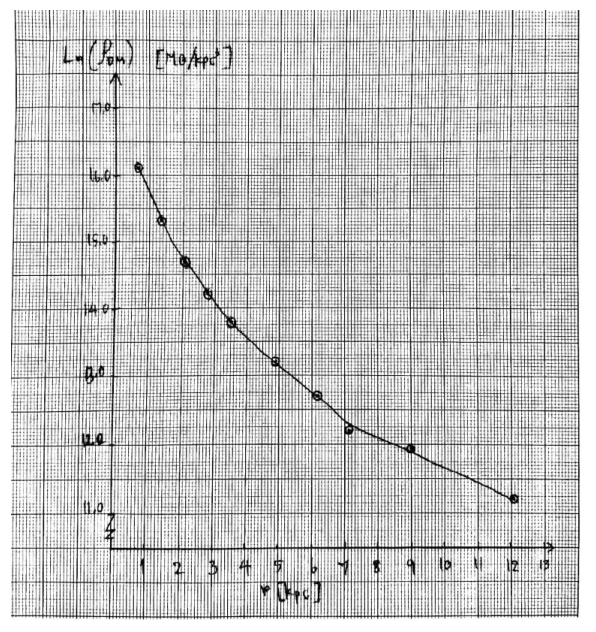
\includegraphics[width=0.57\linewidth]{2017_DA_D2-s4.pdf}
  \end{center}

  Solution 2: $r_c = 3.2\ kpc$

  \begin{center}
  \begin{tabular}{cc}
  $r$ (kpc) & $\ln\left[\rho_{\mathrm{DM}}(r)\right]$
    $\left(\frac{M_\odot}{kpc^3}\right)$\\
  0.70 & 12.79\\
  1.40 & 11.95\\
  2.09 & 11.47\\
  2.79 & 11.21\\
  3.49 & 11.07\\
  4.89 & 11.16\\
  6.25 & 11.26\\
  7.10 & 11.16\\
  9.03 & 11.27\\
  12.05 & 11.41
  \end{tabular}
  \end{center}
  \ioaafig[0.55]{2017_DA_D2-s5.pdf}
\end{description}

\solhead{13.26}{Scaling Relations}
% source id: 2021_DA_DA1
\textbf{Part 1.}

\begin{description}
\item[1.1)] From the plot on the right we can get the equation of the
  straight line as
  \[ y = -0.76\cdot x + 7.32 \]
  \hfill[3 points]

  which taking to the power of 10 is equivalent to:
  $f_g = 10^{7.32}M_*^{-0.76}$, being $f_g$ the gas fraction. Multiplying
  by the stellar mass we finally get:
  \[ M_{gas} = 10^{7.32}\times M_*^{0.24} \]
  \[ a = 10^{7.32} = 2.09\times 10^{7}\ \text{[1 point]};\qquad
     b = 0.24\ \text{[1 point]} \]

\item[1.2)] \hfill[15 points]

  \begin{center}
  \begin{tabular}{cccccc}
  V & LogV & K & Zx & Zy & ZxZy\\
  79.4 & 1.8998 & $-16.8$ & $-1.1778$ & 1.3873 & $-1.6339$\\
  100.1 & 2.0004 & $-19.2$ & $-0.7831$ & 0.4970 & $-0.3892$\\
  158.5 & 2.2000 & $-21.3$ & $-0.0001$ & $-0.2819$ & 0.0000\\
  251.2 & 2.4000 & $-21.4$ & 0.7845 & $-0.3190$ & $-0.2502$\\
  316.2 & 2.5000 & $-24$ & 1.1765 & $-1.2834$ & $-1.5100$\\
  \hline
  Ave & 2.2001 & $-20.54$ & & sum ZxZy & $-3.7833$\\
  St. Dev & 0.2549 & 2.696 & & r & $-0.9458$
  \end{tabular}
  \end{center}

  The best-fit straight line is
  $K = -10\cdot\log_{10}(V_{max}) + 1.47$.
\end{description}

\textbf{Part 2.}

\begin{description}
\item[2.1)] \hfill[10 points]

  Galaxies are at the same distance, therefore the difference in apparent
  magnitudes is the same as in absolute magnitudes, and this relates to a
  luminosity ratio:
  \[ (k_1 - k_2) = (K_1 - K_2)
     = -2.5\times\log_{10}\!\left(\frac{L_1}{L_2}\right) \]
  \hfill[2 points]

  For having the same stellar populations, and ignoring interstellar
  extinction, the luminosity of each galaxy is proportional to its
  stellar mass with the same mass-to-light ratio for both galaxies, such
  that:
  \[ (k_1 - k_2) = -2.5\times\log_{10}
     \!\left(\frac{M_{*1}}{M_{*2}}\right) \]
  \hfill[2 points]

  The difference in magnitudes being 6, we obtain:
  \[ \left(\frac{M_{*1}}{M_{*2}}\right) = 10^{2.4} \]
  \hfill[2 points]

\item[2.2)] \hfill[4 points]

  Using the last result in combination to that of 1A:
  \[ \frac{M_{gas1}}{M_{gas2}}
     = \left(\frac{M_{*1}}{M_{*2}}\right)^{0.24} \]
  \hfill[2 points]
  \[ \frac{M_{gas1}}{M_{gas2}} = 10^{0.576} \]
  \hfill[2 points]

\item[2.3)] \hfill[6 points]

  We found the slope of the TF relation in 1B:
  $\frac{\Delta K}{\Delta\log(V_{max})} = 10$, with $\Delta K = 6$ for
  our galaxies: $\frac{V_{max1}}{V_{max2}} = 10^{0.6}$ [2 points]. Now
  consider the mass distribution as approximately
  spherically-symmetric, giving:
  \[ V_{max} = \sqrt{\frac{G\cdot M_{tot}(<R_{max})}{R_{max}}}, \]
  \hfill[2 points]

  which combined with the ratio just found two lines above leads to:
  \[ \frac{M_{tot1}}{M_{tot2}} = 10^{1.2} \]
  \hfill[2 points]
\end{description}

\textbf{Part 3.} \hfill[15 points]

Baryonic mass is
$M_{Baryonic} = \frac{4.39\times 10^{11}}{7.82}\,[M_\odot]$ and Dark
matter mass is given by
$M_{dm} = 6.82\times\frac{4.39\times 10^{11}}{7.82}\,[M_\odot]$. The
baryonic contribution needs to be decomposed into stellar and gaseous
masses, which is not doable analytically but must be faced numerically,
by tuning the numbers, knowing their sum and knowing the relation between
them from 1.1. The final table looks like this:

\begin{center}
\begin{tabular}{cccccc}
Galaxy & Apparent magnitude $k$ & $M_{gas}$ [$M_\odot$]
  & $M_{*}$ [$M_\odot$] & $M_{dm}$ [$M_\odot$] & $M_{tot}$ [$M_\odot$]\\
$G_1$ & 19.2 & $7.67\times 10^{9}$ & $4.85\times 10^{10}$
  & $3.83\times 10^{11}$ & $4.39\times 10^{11}$
\end{tabular}
\end{center}

Equation to be solved: $1 - k = 0.1415\,k^{0.24}$. This gives
$k = 0.8634$

\textbf{Part 4}

\begin{description}
\item[4.1)] \hfill[4 points]

  We basically found in 2.1 that
  $\left(\frac{M_{*1}}{M_{*2}}\right) = 10^{\frac{\Delta K}{-2.5}}$,
  being $\Delta K = -6$. In this new case, we have the extreme values of
  $\Delta K$ to be $-6.4$ and $-5.6$, therefore the extreme values for
  the exponent are these values divided by $-2.5$, then
  $e\in[2.24,\ 2.56]$

\item[4.2)] \hfill[10 points]

  We have to invert the equation from 1.2 to get:
  $\log_{10}(V_{max}) = -\frac{K}{10} + 0.1467$. Now we can get the
  difference between the measured values and linear-fit predictions,
  approximating numbers to the second digit:

  \begin{center}
  \begin{tabular}{ccccc}
  $K$ [mag] & $V_{max}$ [km/s] & $\log_{10}(V_{max})$ measured
    & $\log_{10}(V_{max})$ from linear fit
    & $|\Delta\log_{10}(V_{max})|$\\
  $-16.8$ & 79.4 & 1.9 & 1.83 & 0.07\\
  $-19.2$ & 100.1 & 2.0 & 2.07 & 0.07\\
  $-21.3$ & 158.5 & 2.2 & 2.28 & 0.08\\
  $-21.4$ & 251.2 & 2.4 & 2.29 & 0.11\\
  $-24.0$ & 316.2 & 2.5 & 2.55 & 0.05
  \end{tabular}
  \end{center}

  Taking two times the RMS of the residuals:
  $\sigma_{stat} = 0.157$

\item[4.3)] With the uncertainties, the expression
  $\log_{10}(V_{max}) = -\frac{K}{10} + 0.1467$ becomes:
  \[ \log_{10}(V_{max}) = -\frac{K}{10} + 0.1467\pm\frac{0.2}{10}
     \pm 0.157 \]
  \hfill[2 points]

  Writing the same expression down for galaxy 1 and 2, subtracting, and
  using $\Delta K = -6$ we get:
  \[ \log_{10}\!\left(\frac{V_{max1}}{V_{max2}}\right)
     = 0.6\pm 0.02\pm 0.157\pm 0.02\pm 0.157 \]
  \hfill[4 points]

  Which leads to the extreme values: $0.954$ and $0.246$.
  \hfill[2 points]

  Finally remembering that circular velocities scale as the square root
  of the total mass, we have to multiply this exponent by 2, getting the
  final answer:
  \[ g\in[0.49,\ 1.91] \]
  \hfill[2 points]
\end{description}

\solhead{13.27}{Galactic Surveys}
% source id: 2022_DA_2
\textbf{Solutions -- Part 1}

\begin{description}
\item[(a)] If we plot given coordinates in XY, XZ and YZ planes we'll see
  the following pictures. See Figures 2, 3 and 4 (0.5p for each graph).
  \ioaafig{2022_DA_2-s1.pdf}
  \ioaafig{2022_DA_2-s2.pdf}
  \ioaafig{2022_DA_2-s3.pdf}
  By observing Figure 2 we can deduce that the group is edge-on and its
  normal lies in XY plane. $X'$ axis is along line of sight so it can be
  calculated by normalizing
  $8.3\hat{i} + 6.2\hat{j} + 1.1\hat{k}$. So
  \[ \hat{x}' = 0.79667866\,\hat{i} + 0.59510936\,\hat{j}
     + 0.10558392\,\hat{k} \]
  (0.5p) $Z'$ axis lays in XY plane and is perpendicular to $X'$ so it
  can be calculated by normalizing $\hat{x}'\times\hat{k}$
  \[ \hat{z}' = 0.59845448\,\hat{i} - 0.80115681\,\hat{j} \]
  \hfill(2p)

\item[(b)] One can choose $x'$ as line of sight (found in part (a)) (1p):
  \[ \hat{x}' = 0.79667866\,\hat{i} + 0.59510936\,\hat{j}
     + 0.10558392\,\hat{k} \]
  $z'$ can be chosen as halo disk normal (found in part (a)) (1p):
  \[ \hat{z}' = 0.59845448\,\hat{i} - 0.80115681\,\hat{j} \]
  And finally for $y'$ (1p):
  \[ \hat{y}' = \hat{x}'\times\hat{z}'
     = 0.08458928\,\hat{i} + 0.06318717\,\hat{j} - 0.9944104\,\hat{k} \]

\item[(c)] Each coordinate in $X'Y'Z'$ system can be found by following
  equations
  \begin{align*}
  x' &= \hat{x}'\cdot(\vec{r} - \vec{r}_c)\\
  y' &= \hat{y}'\cdot(\vec{r} - \vec{r}_c)\\
  z' &= \hat{z}'\cdot(\vec{r} - \vec{r}_c)
  \end{align*}
  Where $\hat{x}'$, $\hat{y}'$ and $\hat{z}'$ are unit vectors of local
  $X'Y'Z'$ system, $\vec{r}$ is coordinate of a galaxy and $\vec{r}_c$
  is coordinate of the center.

  This values are calculated in the following table (0.5p for each
  correct $x'$, $y'$, $z'$ tuple):

  \begin{center}
  \begin{tabular}{rrrrrrr}
  & $x - x_c$ & $y - y_c$ & $z - z_c$ & $x'$ & $y'$ & $z'$\\
  1 & 0.101124 & 0.109271 & 0.294476 & 0.176684 & $-0.277372$ & $-0.027025$\\
  2 & 1.582909 & 0.989392 & 0.405895 & 1.892722 & $-0.207212$ & 0.154641\\
  3 & 0.582735 & 0.213285 & 1.126426 & 0.710112 & $-1.057359$ & 0.177866\\
  4 & 0.144328 & 0.369381 & 1.338567 & 0.476137 & $-1.295537$ & $-0.209558$\\
  5 & $-0.517770$ & $-0.151687$ & $-1.458202$ & $-0.656729$ & 1.396668 & $-0.188336$\\
  6 & 0.480059 & 0.105110 & 1.362674 & 0.588881 & $-1.307808$ & 0.203084\\
  7 & $-0.309855$ & $-0.319116$ & $-0.568033$ & $-0.496739$ & 0.518483 & 0.070227\\
  8 & 0.239541 & 0.188218 & $-0.730736$ & 0.225694 & 0.758807 & $-0.007438$\\
  9 & $-0.324800$ & $-0.169551$ & 0.116378 & $-0.347375$ & $-0.153915$ & $-0.058541$\\
  10 & $-1.227659$ & $-0.768684$ & $-0.612379$ & $-1.500158$ & 0.456538 & $-0.118862$\\
  11 & $-0.263209$ & $-0.234869$ & $-0.485227$ & $-0.400698$ & 0.445410 & 0.030649\\
  12 & 0.381200 & 0.282515 & $-0.365581$ & 0.433222 & 0.413634 & 0.001792\\
  13 & $-1.185021$ & $-0.941303$ & 0.302593 & $-1.472310$ & $-0.460620$ & 0.044950\\
  14 & 1.286640 & 0.930147 & $-0.777889$ & 1.496445 & 0.941150 & 0.024802\\
  15 & $-0.106760$ & $-0.095804$ & $-0.184997$ & $-0.161600$ & 0.168879 & 0.012863\\
  16 & $-0.686865$ & $-0.352750$ & 0.566244 & $-0.697350$ & $-0.643470$ & $-0.128449$
  \end{tabular}
  \end{center}

\item[(d)] Spherical coordinates can by calculated by following
  relations:
  \[ r = \sqrt{x'^2 + y'^2 + z'^2} \]
  \[ \phi = \arctan\frac{y'}{x'}\ \text{and signs of $x'$ and $y'$} \]
  \[ \theta = \arccos\frac{z}{r} \]
  Calculated values are given in the following table (0.5p for each
  correct $r$, $\phi$, $\theta$ tuple):

  \begin{center}
  \begin{tabular}{rrrrrrr}
  & $x'$ & $y'$ & $z'$ & $r$ & $\phi$ & $\theta$\\
  1 & 0.176684 & $-0.277372$ & $-0.027025$ & 0.329974 & 5.279566 & 1.652789\\
  2 & 1.892722 & $-0.207212$ & 0.154641 & 1.910301 & 6.174141 & 1.489757\\
  3 & 0.710112 & $-1.057359$ & 0.177866 & 1.286042 & 5.303793 & 1.432047\\
  4 & 0.476137 & $-1.295537$ & $-0.209558$ & 1.396079 & 5.064586 & 1.721471\\
  5 & $-0.656729$ & 1.396668 & $-0.188336$ & 1.554814 & 2.010330 & 1.692226\\
  6 & 0.588881 & $-1.307808$ & 0.203084 & 1.448581 & 5.135477 & 1.430138\\
  7 & $-0.496739$ & 0.518483 & 0.070227 & 0.721461 & 2.334780 & 1.473302\\
  8 & 0.225694 & 0.758807 & $-0.007438$ & 0.791695 & 1.281697 & 1.580191\\
  9 & $-0.347375$ & $-0.153915$ & $-0.058541$ & 0.384430 & 3.558678 & 1.723672\\
  10 & $-1.500158$ & 0.456538 & $-0.118862$ & 1.572587 & 2.846171 & 1.646452\\
  11 & $-0.400698$ & 0.445410 & 0.030649 & 0.599906 & 2.303400 & 1.519685\\
  12 & 0.433222 & 0.413634 & 0.001792 & 0.598981 & 0.762273 & 1.567805\\
  13 & $-1.472310$ & $-0.460620$ & 0.044950 & 1.543336 & 3.444801 & 1.541667\\
  14 & 1.496445 & 0.941150 & 0.024802 & 1.767973 & 0.561416 & 1.556768\\
  15 & $-0.161600$ & 0.168879 & 0.012863 & 0.234094 & 2.334171 & 1.515821\\
  16 & $-0.697350$ & $-0.643470$ & $-0.128449$ & 0.957522 & 3.886829 & 1.705349
  \end{tabular}
  \end{center}

\item[(e)] Using radii calculated above and number of galaxies for each
  data one can calculate number of galaxies in each bin. Range of bin 1
  is (0.2, 0.425), bin 2 -- (0.425, 0.65) and so on bin 8 --
  (1.775, 2.0).

  Correct values for each bin are: (0.5p for each correct $n$)

  \begin{center}
  \begin{tabular}{rrr}
  & Center of the bin & Number of the galaxies\\
  1 & 0.312500 & 624\\
  2 & 0.537500 & 451\\
  3 & 0.762500 & 354\\
  4 & 0.987500 & 293\\
  5 & 1.212500 & 253\\
  6 & 1.437500 & 210\\
  7 & 1.662500 & 174\\
  8 & 1.887500 & 170
  \end{tabular}
  \end{center}
  \ioaafig{2022_DA_2-s4.pdf}

  In order to get probability density function each value of histogram
  must be divided by it integral on the whole region. The integral can
  be approximated by finding total area of the rectangles:
  \[ I = \sum_{n=1}^{8}H(r_i)\,d = 569.025 \]
  Where $d = 0.225$ is size of a bin. After dividing each data by $I$ we
  get (0.25p for each correct probability density):

  \begin{center}
  \begin{tabular}{rrrr}
  & Center of the bin & Number of the galaxies & Probability density\\
  1 & 0.312500 & 624 & 1.096613\\
  2 & 0.537500 & 451 & 0.792584\\
  3 & 0.762500 & 354 & 0.622117\\
  4 & 0.987500 & 293 & 0.514916\\
  5 & 1.212500 & 253 & 0.444620\\
  6 & 1.437500 & 210 & 0.369052\\
  7 & 1.662500 & 174 & 0.305786\\
  8 & 1.887500 & 170 & 0.298757
  \end{tabular}
  \end{center}
  \ioaafig{2022_DA_2-s5.pdf}

\item[(f)] Since histogram equation has following form:
  \[ H(r) = \frac{1}{A + B\cdot r} \]
  We should calculate $1/H(r)$ which gives the following values (0.125
  for each correct $1/H$):

  \begin{center}
  \begin{tabular}{rrrr}
  & $r$ & $H(r)$ & $1/H(r)$\\
  1 & 0.312500 & 624 & 0.001603\\
  2 & 0.537500 & 451 & 0.002217\\
  3 & 0.762500 & 354 & 0.002825\\
  4 & 0.987500 & 293 & 0.003413\\
  5 & 1.212500 & 253 & 0.003953\\
  6 & 1.437500 & 210 & 0.004762\\
  7 & 1.662500 & 174 & 0.005747\\
  8 & 1.887500 & 170 & 0.005882
  \end{tabular}
  \end{center}
  \ioaafig{2022_DA_2-s6.pdf}

  Finding the slope and the intercept of this line (by graph or any
  other method) gives following values:
  \[ A = 0.00065977;\qquad B = 0.00285494 \]
\end{description}

\textbf{Solutions -- Part 2}

\begin{description}
\item[(a)] We can $\phi$ values from Part 1.c to distribute them in 60
  degree bins.
  % sic: "We can phi values" as in source (missing "use")
  In bin 1 we have number of galaxies which fall in (0, 60) degree
  range, in bin 2 -- (60, 120) and so on bin 6 -- (300, 360).

  Part 1.c data in degrees:

  \begin{center}
  \begin{tabular}{rrr}
  & Angle & Number of galaxies\\
  1 & 302.496846 & 291\\
  2 & 353.752245 & 170\\
  3 & 303.884926 & 253\\
  4 & 290.179429 & 8\\
  5 & 115.183442 & 72\\
  6 & 294.241133 & 120\\
  7 & 133.773013 & 302\\
  8 & 73.435830 & 52\\
  9 & 203.897219 & 28\\
  10 & 163.073590 & 40\\
  11 & 131.975076 & 72\\
  12 & 43.675004 & 379\\
  13 & 197.372555 & 82\\
  14 & 32.166754 & 62\\
  15 & 133.738158 & 305\\
  16 & 222.698869 & 293
  \end{tabular}
  \end{center}

  We get the following data for the histogram (0.5p for each correct
  $n$):

  \begin{center}
  \begin{tabular}{rrr}
  & Center of the bin & Number of galaxies\\
  1 & 30 & 441\\
  2 & 90 & 124\\
  3 & 150 & 719\\
  4 & 210 & 403\\
  5 & 270 & 128\\
  6 & 330 & 714
  \end{tabular}
  \end{center}

  Uniform value is total number of galaxies divides by 6 which is
  421.5. Square deviation is $241^\circ$ (1p)
  \ioaafig{2022_DA_2-s7.pdf}

\item[(b)] A galaxy with the orbital radius $r$ around central mass $M$
  has velocity (2p):
  \[ v = \sqrt{\frac{GM}{r}} \]
  This will cause to give the following error in distance along line of
  sight (2p):
  \[ d = \frac{v}{H} = \frac{1}{H}\sqrt{\frac{GM}{r}} \]
  Angle difference for galaxies at 90 and 270 degrees will be (2p):
  \[ \alpha = \arctan\frac{d}{r}
     = \arctan\frac{1}{H}\sqrt{\frac{GM}{r^3}} \]
  \ioaafig{2022_DA_2-s8.pdf}

\item[(c)] Galaxies originally in bins of range (60, 120) and (240, 300)
  might move to (120, 180) and (300, 360) respectively. So we should
  subtract correction value found in previous task to the galaxies in
  bins 2 and 5 to see if they move to bins 1 and 4 respectively. (0.25p
  for each correct corrected angle)

  \begin{center}
  \begin{tabular}{rrrr}
  & Original angle & Corrected angle & Number of galaxies\\
  1 & 302.494665 & 276.136451 & 291\\
  2 & 353.752069 & 351.714594 & 170\\
  3 & 303.884728 & 300.199512 & 253\\
  4 & 290.178642 & 290.178642 & 8\\
  5 & 115.184577 & 115.184577 & 72\\
  6 & 294.241835 & 294.241835 & 120\\
  7 & 133.776280 & 125.061576 & 302\\
  8 & 73.437747 & 73.437747 & 52\\
  9 & 203.899065 & 203.899065 & 28\\
  10 & 163.073490 & 160.346665 & 40\\
  11 & 131.977481 & 120.548626 & 72\\
  12 & 43.676971 & 43.676971 & 379\\
  13 & 197.372956 & 197.372956 & 82\\
  14 & 32.167948 & 32.167948 & 62\\
  15 & 133.743596 & 94.077612 & 305\\
  16 & 222.694636 & 222.694636 & 293
  \end{tabular}
  \end{center}

  New corrected distribution looks like this (0.3p for each correct
  $n$):

  \begin{center}
  \begin{tabular}{rrr}
  & Center of the bin & Number of galaxies\\
  1 & 30 & 441\\
  2 & 90 & 429\\
  3 & 150 & 414\\
  4 & 210 & 403\\
  5 & 270 & 419\\
  6 & 330 & 423
  \end{tabular}
  \end{center}

  In this case square deviation equals to $12^\circ$ (1p)
  \ioaafig{2022_DA_2-s9.pdf}
\end{description}

\textbf{Solutions -- Part 3}

\begin{description}
\item[(a)] With simple combinatorics one can get (0.6p for each correct
  $N$):
  \begin{align*}
  N_{CC} &= N_C(N_C - 1) = 249500\\
  N^{*}_{CS} &= N_C N_S = 500000\\
  N_{CS} &= N_C(N_C - 1)N_S = 249500000\\
  N^{*}_{SS} &= N_C N_S(N_S - 1) = 499500000\\
  N_{SS} &= N_C N_S(N_C - 1)N_S = 249500000000
  \end{align*}

\item[(b)] We can calculate all probability densities using
  center-center and center-satellite densities. Non-normalized values
  (with $c_1 = c_2 = c_3 = 1$) are calculated in the following table
  (0.5p for each correct tuple):

  \begin{center}
  \begin{tabular}{rrrrrrr}
  & $r$ & $\rho^{*}_{CS}$ & $\rho_{CC}$ & $\rho^{*}_{SS}$
    & $\rho_{SS}$ & $\rho_{CS}$\\
  1 & 0.312500 & 1.096613 & 0.406141 & 0.375800 & 17.365137 & 0.975747\\
  2 & 0.537500 & 0.792584 & 0.807863 & 0.337652 & 12.992898 & 0.994072\\
  3 & 0.762500 & 0.622117 & 1.340510 & 0.295110 & 8.653487 & 0.988565\\
  4 & 0.987500 & 0.514916 & 1.134011 & 0.261824 & 8.568351 & 0.837480\\
  5 & 1.212500 & 0.444620 & 0.478630 & 0.239696 & 10.729180 & 0.638199\\
  6 & 1.437500 & 0.369052 & 0.143154 & 0.195787 & 10.112507 & 0.458355\\
  7 & 1.662500 & 0.305786 & 0.073165 & 0.155452 & 8.262279 & 0.352612\\
  8 & 1.887500 & 0.298757 & 0.060971 & 0.168470 & 8.998531 & 0.379962
  \end{tabular}
  \end{center}

  For normalization (same way as in Part 1.d) we get $c_1 = 2.18592$;
  $c_2 = 0.79304$; $c_3 = 0.0516$. Multiplying relevant densities by
  this values gives (0.5p for each correct normalized tuple):

  \begin{center}
  \begin{tabular}{rrrrr}
  & $r$ & $\rho^{*}_{SS}$ & $\rho_{SS}$ & $\rho_{CS}$\\
  1 & 0.312500 & 0.822854 & 0.900750 & 0.770962\\
  2 & 0.537500 & 0.739325 & 0.673957 & 0.785441\\
  3 & 0.762500 & 0.646175 & 0.448866 & 0.781089\\
  4 & 0.987500 & 0.573292 & 0.444450 & 0.661713\\
  5 & 1.212500 & 0.524839 & 0.556535 & 0.504257\\
  6 & 1.437500 & 0.428697 & 0.524548 & 0.362158\\
  7 & 1.662500 & 0.340380 & 0.428574 & 0.278607\\
  8 & 1.887500 & 0.368883 & 0.466764 & 0.300217
  \end{tabular}
  \end{center}
  \ioaafig{2022_DA_2-s10.pdf}
  \ioaafig{2022_DA_2-s11.pdf}
  \ioaafig{2022_DA_2-s12.pdf}
  \ioaafig{2022_DA_2-s13.pdf}

\item[(c)] Total probability density is weighted sum of all densities
  (4p):
  \[ \rho \sim \frac{N_{CC}\rho_{CC} + N^{*}_{CS}\rho^{*}_{CS}
     + N_{CS}\rho_{CS} + N^{*}_{SS}\rho^{*}_{SS} + N_{SS}\rho_{SS}}
     {N_{CC} + N^{*}_{CS} + N_{CS} + N^{*}_{SS} + N_{SS}} \]

  Calculated values and normalized densities are given in the following
  table:

  \begin{center}
  \begin{tabular}{rrrr}
  & $r$ & Calculated $\rho$ & Normalized $\rho$\\
  1 & 0.312500 & 0.004212 & 0.843662\\
  2 & 0.537500 & 0.003606 & 0.722433\\
  3 & 0.762500 & 0.002967 & 0.594357\\
  4 & 0.987500 & 0.002693 & 0.539524\\
  5 & 1.212500 & 0.002663 & 0.533361\\
  6 & 1.437500 & 0.002265 & 0.453652\\
  7 & 1.662500 & 0.001813 & 0.363239\\
  8 & 1.887500 & 0.001968 & 0.394216
  \end{tabular}
  \end{center}
  \ioaafig{2022_DA_2-s14.pdf}

  Most similar to this density is plot E on Figure 1 (1p).
\end{description}

\chapter{Gravitational Waves}

\section*{Theory problems}

\probhead{14.1}{Gravitational Waves}{2016}{Bhubaneswar, India}{TH T11}{50}
% source id: 2016_TH_T11   tag: GW frequency at merger MS/WD/NS/BH
The first signal of gravitational waves was observed by two advanced LIGO
detectors at Hanford and Livingston, USA in September 2015. One of these
measurements (strain vs.\ time in seconds) is shown in the accompanying figure.
In this problem, we will interpret this signal in terms of a small test mass $m$
orbiting around a large mass $M$ (i.e.\ $m \ll M$), by considering several
models for the nature of the central mass.

\ioaafig{2016_TH_T11-f1.pdf}

The test mass loses energy due to the emission of gravitational waves. As a
result the orbit keeps on shrinking, until the test mass reaches the surface of
the object, or in the case of a black hole, the innermost stable circular orbit
--- ISCO --- which is given by $R_{\mathrm{ISCO}} = 3R_{\mathrm{sch}}$, where
$R_{\mathrm{sch}}$ is the Schwarzschild radius of the black hole. This is the
``epoch of merger''. At this point, the amplitude of the gravitational wave is
maximum, and so is its frequency, which is always twice the orbital frequency.
In this problem, we will only focus on the gravitational waves before the
merger, when Kepler's laws are assumed to be valid. After the merger, the form
of gravitational waves will drastically change.

\begin{description}
\item[(T11.1)] Consider the observed gravitational waves shown in the figure
  above. Estimate the time period, $T_0$, and hence calculate the frequency,
  $f_0$, of gravitational waves just before the epoch of merger. \hfill[7]
\item[(T11.2)] For any main sequence (MS) star, the radius of the star,
  $R_{\mathrm{MS}}$, and its mass, $M_{\mathrm{MS}}$, are related by a power
  law. Find the highest frequency of emitted gravitational waves,
  $f_{\mathrm{MS,max}}$, if the test mass is orbiting a main sequence star.
\item[(T11.3)] Find the highest frequency of emitted gravitational waves,
  $f_{\mathrm{WD,max}}$, if the test mass is orbiting a white dwarf. Take the
  radii of white dwarfs to be in the range $\sim 3000$ to $6000$\,km.
\item[(T11.4)] Neutron stars (NS) are a peculiar type of compact objects which
  have masses between $1$ and $3M_\odot$ and radii in the range $10$--$15$\,km.
  Find the range of frequencies of emitted gravitational waves,
  $f_{\mathrm{NS,min}}$ and $f_{\mathrm{NS,max}}$, if the test mass is orbiting
  a neutron star at a distance close to the neutron star radius.
\item[(T11.5)] If the test mass is orbiting a black hole (BH), write the
  expression for the frequency of emitted gravitational waves,
  $f_{\mathrm{BH}}$, in terms of the mass of the black hole,
  $M_{\mathrm{BH}}$, and the solar mass $M_\odot$. \hfill[5]
\item[(T11.6)] Based only on the time period (or frequency) of gravitational
  waves before the epoch of merger, determine whether the central object can be
  a main sequence star (MS), a white dwarf (WD), a neutron star (NS), or a
  black hole (BH). Estimate the mass of this object, $M_{\mathrm{obj}}$, in
  units of $M_\odot$. \hfill[8]
\end{description}

\probhead{14.2}{LIGO}{2021}{Bogot\'a (remote)}{TH Q1}{5}
% source id: 2021_TH_Q1   tag: BH-merger GW energy vs supernova
The first detection of gravitational waves GW150914 was announced in 2016 by
the collaboration LIGO (Laser Interferometer Gravitational-Wave Observatory).
The detected signal corresponds to the merger of two black holes with masses of
$35M_\odot$ and $30M_\odot$, which when joined formed a black hole of
$62M_\odot$. Ignoring the rotational energies of the black holes, you may assume
that the energy released by this process ($E_{GW}$) is emitted solely in the
form of gravitational waves, that were observed by the interferometer in 2015.
You are given that the explosion of a supernova (SN) releases
$E_{SN} = 2 \times 10^{44}$\,J.

\begin{description}
\item[(1.1)] To find out which of these two events (SN, GW) releases more
  energy, estimate the energy ratio $E_{SN}/E_{GW}$. \hfill[5.0\,pt]
\end{description}

\probhead{14.3}{LISA}{2023}{Katowice, Poland}{TH Q13}{45}
% source id: 2023_TH_Q13   tag: white-dwarf binary GW strain, chirp mass
The Laser Interferometer Space Antenna (LISA) is a proposed experiment to detect
low-frequency gravitational waves. It consists of three spacecraft arranged in
an equilateral triangle. A passing gravitational wave changes the distance
between the spacecraft, which can be precisely measured (more details are given
in the notes below).

One of the sources of low-frequency gravitational waves are compact binary star
systems, for example binary white dwarfs. Such a system was recently discovered
at a distance of $2.34$\,kpc from the Sun. The orbital period of the binary was
found to be $414.79$\,s and is changing at a rate of
$-7.49 \times 10^{-4}$\,s\,yr$^{-1}$ due to the emission of gravitational waves.

\begin{description}
\item[(a)] Check if this binary system can be detected by LISA. \hfill[25 points]
\item[(b)] Calculate the chirp mass. \hfill[5 points]
\item[(c)] Determine the masses of both components knowing that the ratio
  between the radius of one of the components to the semi-major axis of the
  orbit is $0.139$, and assuming both components follow the mass--radius
  relation for white dwarfs given in the table below. \hfill[15 points]
\end{description}

\noindent\textbf{Notes:}
\begin{enumerate}
\item A binary star system with an orbital period $P$ emits gravitational waves
  with a frequency of $f = 2/P$.
\item LISA measures a dimensionless quantity called the characteristic strain
  amplitude, $S$, given by
  \[ S = h\sqrt{f T_{\mathrm{obs}}}, \]
  where $T_{\mathrm{obs}} = 4$\,yr is the expected duration of the mission. $h$
  is the gravitational wave strain, given by
  \[ h = \frac{2(G\mathcal{M})^{5/3}(\pi f)^{2/3}}{c^4 D}, \]
  where $\mathcal{M}$ is the so-called chirp mass, $f$ is the frequency of the
  gravitational wave and $D$ is the distance to the system. If we denote the
  masses of the components by $M_1$ and $M_2$, then the chirp mass is given by
  \[ \mathcal{M} = \frac{(M_1 M_2)^{3/5}}{(M_1 + M_2)^{1/5}}. \]
  The expected sensitivity of LISA as a function of gravitational wave
  frequency is presented in the figure below.
\item The semi-major axis $a$ of the binary system changes due to the emission
  of gravitational waves at a rate
  \[ \frac{\Delta a}{\Delta t} = -\frac{64}{5}\,\frac{G^3}{c^5}\,
     \frac{M_1 M_2 (M_1 + M_2)}{a^3}. \]
\end{enumerate}

\ioaafig{2023_TH_Q13-f2.pdf}

\probhead{14.4}{Gravitational Waves}{2025}{Mumbai, India}{TH T03}{15}
% source id: 2025_TH_T03   tag: binary BH chirp, merger time
Orbiting binary black holes generate gravitational waves. Consider two black
holes, in our Galaxy, with masses $M = 36\,M_\odot$ and $m = 29\,M_\odot$,
revolving in circular orbits with orbital angular frequency $\omega$ around
their centre of mass.

\begin{description}
\item[(T03.1)] Assuming Newtonian gravity, derive an expression for the angular
  frequency, $\omega_{\mathrm{ini}}$, of the black hole orbits at a time
  $t_{\mathrm{ini}}$, when the separation between the black holes was $4.0$
  times the sum of their Schwarzschild radii, in terms of only $M$, $m$, and
  physical constants. Calculate the value of $\omega_{\mathrm{ini}}$
  (in rad\,s$^{-1}$). \hfill[5]
\item[(T03.2)] In general relativity, black holes in orbit emit gravitational
  waves with frequency $f_{\mathrm{GW}}$, such that
  $2\pi f_{\mathrm{GW}} = \omega_{\mathrm{GW}} = 2\omega$. This shrinks the
  black hole orbits, which in turn increases $f_{\mathrm{GW}}$. The rate of
  change of $f_{\mathrm{GW}}$ is
  \[ \frac{\mathrm{d}f_{\mathrm{GW}}}{\mathrm{d}t}
     = \frac{96\pi^{8/3}}{5}\,G^{5/3} c^{\beta}
       \mathcal{M}_{\mathrm{chirp}}^{\alpha/3} f_{\mathrm{GW}}^{\delta/3}, \]
  where $\mathcal{M}_{\mathrm{chirp}} = \dfrac{(mM)^{3/5}}{(m+M)^{1/5}}$ is
  called the ``chirp mass''. Find the values of $\alpha$, $\beta$ and $\delta$.
  \hfill[4]
\item[(T03.3)] Assume that the gravitational waves associated with the event
  were first detected at time $t_{\mathrm{ini}} = 0$. Derive an expression for
  the observed time of black hole merger, $t_{\mathrm{merge}}$, when
  $f_{\mathrm{GW}}$ becomes very large, in terms of $\omega_{\mathrm{ini}}$,
  $\mathcal{M}_{\mathrm{chirp}}$, and physical constants only. Calculate the
  value of $t_{\mathrm{merge}}$ (in seconds). \hfill[6]
\end{description}

\section*{Data-analysis problems}

\probhead{14.5}{Gravitational wave astronomy}{2022}{Kutaisi, Georgia}{DA 1}{45}
% source id: 2022_DA_1   tag: GW170817 chirp mass from f(t)
In this problem, we will analyze frequency vs.\ time representations of data
containing the gravitational wave event GW170817, which was the first
observation by LIGO of a merger of a binary neutron star system.

\ioaafig{2022_DA_1-f1.pdf}

\subsection*{1.1 Data from the graph}
\begin{description}
\item[(1.1.1)] You are given a semi-logarithmic graph, from which you need to
  extract values of frequency and time. Let the bottom left corner be the
  origin $(0,0)$, horizontal coordinate $x$ is measured in centimetres. Find a
  linear expression to obtain actual time $t$ from $x$. \hfill[2\,pt]
\item[(1.1.2)] Similarly, find an expression for the frequency $f$ as a
  function of the vertical coordinate $y$ measured in centimetres.
  \hfill[3\,pt]
\item[(1.1.3)] Extract 14 values of time and corresponding frequency from the
  given graph into a table. At least one of the values should correspond to a
  frequency more than $100$\,Hz. \hfill[7\,pt]
\end{description}

\subsection*{1.2 Calculate system parameters}
The most plausible explanation for this evolution of frequency is the
in-spiraling of two orbiting masses, $m_1$ and $m_2$, due to gravitational-wave
emission. At the lower frequencies, such evolution is characterized by the
``chirp mass''
\[ M_{\mathrm{chirp}} = \frac{(m_1 m_2)^{3/5}}{(m_1+m_2)^{1/5}}
   = \frac{c^3}{G}\left[\frac{5}{96}\,\pi^{-8/3} f^{-11/3}\dot{f}\right]^{3/5}, \]
where $f$ and $\dot{f}$ are the observed frequency and its rate of change with
respect to time, and $G$ and $c$ are the gravitational constant and the speed
of light.

\begin{description}
\item[(1.2.1)] From the equation above, derive an expression for the frequency
  dependence on time. \hfill[3\,pt]\\
  \textit{Note:} if $x^n \dot{x} = k$, then $\dfrac{x^{n+1}}{n+1} = kt + C$,
  where $k$, $n$ and $C$ are constants.
\item[(1.2.2)] By plotting the appropriate graph, find the chirp mass and
  estimate its error caused by uncertainty in the slope calculation.
  \hfill[22\,pt]
\end{description}

We realize that what is measured by the ground-based GW detectors are actually
the detector-frame masses, which are related to the source-frame masses by
\[ m_{\mathrm{detector}} = (1+z)\,m, \]
where $z$ is the redshift of the binary.

\begin{description}
\item[(1.2.3)] If the host galaxy NGC 4993 has a redshift $z = 0.009783$, find
  the source-frame chirp mass. \hfill[2\,pt]
\item[(1.2.4)] The mass ratio $q = m_1/m_2$ is much harder to measure. Advanced
  waveform analysis constrains this ratio; using the chirp mass found above,
  determine the range of possible values of the individual masses $m_1$ and
  $m_2$. \hfill[6\,pt]
\end{description}

\clearpage
\section*{Solutions to Chapter 14}

\solhead{14.1}{Gravitational Waves}
% source id: 2016_TH_T11
\begin{description}
\item[(T11.1)] From the graph, just before the peak of emission, the time
  period of gravitational waves is approximately $(0.007 \pm 0.004)$\,s.
  \[ T_0 \approx 0.007\,\mathrm{s} \]
  \hfill(2 points)

  That is, the frequency of the gravitational waves is
  $f_0 \approx 142.86$\,Hz. \hfill(1 point)

\item[(T11.2)] Since $m \ll M$ then, by Kepler's third law
  \[ f_{\mathrm{orbital}} = \frac{1}{2\pi}\sqrt{\frac{GM}{r^3}} \]
  \hfill(4 points)

  Hence the frequency of the gravitational waves is
  \[ f_{\mathrm{grav}} = 2 f_{\mathrm{orbital}}
     = \frac{1}{\pi}\sqrt{\frac{GM}{r^3}} \]
  \hfill(1 point)

  The frequency will be maximum when $r = R_{\mathrm{MS}}$. \hfill(1 point)

  For main sequence stars,
  \[ \frac{R_{\mathrm{MS}}}{R_\odot}
     = \left(\frac{M_{\mathrm{MS}}}{M_\odot}\right)^{\alpha}
     \qquad\therefore\quad R_{\mathrm{MS}}
     = R_\odot \left(\frac{M_{\mathrm{MS}}}{M_\odot}\right)^{\alpha} \]
  \hfill(1 point)
  \begin{align*}
    \therefore f_{\mathrm{MS}}
      &= \frac{1}{\pi}\sqrt{\frac{G M_{\mathrm{MS}}}{R_\odot^3}}
         \left(\frac{M_\odot}{M_{\mathrm{MS}}}\right)^{3\alpha/2} \\
      &= \frac{1}{\pi}\sqrt{\frac{G M_\odot}{R_\odot^3}}
         \left(\frac{M_\odot}{M_{\mathrm{MS}}}\right)^{(3\alpha-1)/2} \\
    f_{\mathrm{MS}}
      &= \frac{1}{\pi}\sqrt{\frac{G M_\odot}{R_\odot^3}}
         \left(\frac{M_{\mathrm{MS}}}{M_\odot}\right)^{(1-3\alpha)/2}
  \end{align*}
  \hfill(3 points)

\item[(T11.3)] For possible values of $\alpha$ given in the question, the
  exponent $\frac{1-3\alpha}{2}$ is negative. Thus, if
  $M_{\mathrm{MS}} > M_\odot$, the frequency will be smaller. Thus, for highest
  possible frequency coming from a main sequence star, you should take lowest
  possible mass i.e.\ $\alpha = 1.0$. \hfill(4 points)
  \begin{align*}
    f_{\mathrm{MS,max}}
      &= \frac{1}{\pi}\sqrt{\frac{G M_\odot}{R_\odot^3}}
         \left(\frac{M_{\mathrm{MS}}}{M_\odot}\right)^{\left(\frac{1-3\times 1}{2}\right)} \\
      &= \frac{1}{\pi}\sqrt{\frac{G M_\odot}{R_\odot^3}}
         \times \frac{M_\odot}{M_{\mathrm{MS}}}
  \end{align*}
  \hfill(2 points)

  The frequency of gravitational waves will be given by,
  \begin{align*}
    f_{\mathrm{MS,max}}
      &= \frac{1}{\pi}\sqrt{\frac{6.674 \times 10^{-11} \times 1.989 \times 10^{30}}
         {(6.955 \times 10^{8})^{3}}} \times \frac{1}{0.08} \\
    f_{\mathrm{MS,max}} &= 2.5\,\mathrm{mHz}
  \end{align*}
  \hfill(3 points)

\item[(T11.4)] The maximum frequency would be when $r = R_{\mathrm{WD}}$.
  \hfill(1 point)

  We use the notation $R_{WD\odot}$ for the radius of a solar mass white
  dwarf. Then for white dwarfs
  % sic: the official solution prints the mass ratio below as M_WD/M_sun;
  % from R \propto M^{-1/3} it should be M_sun/M_WD, which is what the
  % subsequent lines (and the numerical answer) actually use.
  \[ R_{WD}^3 = R_{WD\odot}^3 \frac{M_{WD}}{M_\odot} \]
  \hfill(1 point)
  \begin{align*}
    f_{\mathrm{WD}}
      &= \frac{1}{\pi}\sqrt{\frac{G M_{\mathrm{WD}}}{R_{WD}^3}} \\
      &= \frac{1}{\pi}\sqrt{\frac{G M_\odot}{R_{WD\odot}^3}}\,
         \frac{M_{WD}}{M_\odot}
  \end{align*}
  \hfill(2 points)

  For maximum frequency, we have to take highest white dwarf mass.
  \hfill(2 points)
  \begin{align*}
    f_{\mathrm{WD,max}}
      &= 2.600 \times 10^{-6} \times
         \sqrt{\frac{1.989 \times 10^{30}}{(6000 \times 10^{3})^{3}}}
         \times 1.44 \\
      &= 2.600 \times 10^{-6} \times 95.96 \times 10^{3} \times 1.44 \\
    f_{\mathrm{WD,max}} &= 0.359\,\mathrm{Hz}
  \end{align*}
  \hfill(2 points)

\item[(T11.5)]
  \[ f_{grav} = \frac{1}{\pi}\sqrt{\frac{G M_{\mathrm{NS}}}{R_{\mathrm{NS}}^3}} \]
  The lowest possible frequency is when $M_{\mathrm{NS}}$ is lowest and
  $R_{\mathrm{NS}}$ is the highest. \hfill(2 points)

  For $M_{\mathrm{NS}} = M_\odot$ and $R = 15$\,km, we get
  \[ f_{\mathrm{NS,min}} = 1.996\,\mathrm{kHz} \]
  \hfill(2 points)

  Similarly, the largest possible frequency is when $M_{\mathrm{NS}}$ is the
  largest and $R_{\mathrm{NS}}$ is the smallest. \hfill(2 points)

  For $M_{\mathrm{NS}} = 3M_\odot$ and $R = 10$\,km, we get
  \[ f_{\mathrm{NS,max}} = 6.352\,\mathrm{kHz} \]
  \hfill(2 points)

\item[(T11.6)] For black holes, we have to consider $R_{ISCO}$.
  \hfill(2 points)

  Hence the equation will be,
  \[ f_{BH} = \frac{1}{\pi} \times
     \sqrt{\frac{G M_\odot}{27 R_{sch-\odot}^3}} \times
     \frac{M_\odot}{M_{BH}} \]
  \hfill(2 points)
  \[ f_{BH} = 4.396\,\mathrm{kHz} \times \frac{M_\odot}{M_{BH}} \]
  \hfill(3 points)

\item[(T11.7)] We found the frequency of the LIGO-detected wave to be
  166.67\,Hz just before merger.
  % sic: the official solution says 166.67 Hz here, although part (T11.1)
  % found 142.86 Hz (and 142.86 is used in the mass estimate below).
  As per our analysis above, only black holes can lead to emission in this
  frequency range: Black Hole. \hfill(2 points)

  By using corresponding expression,
  \[ M_{\mathrm{obj}} = \frac{4396}{142.86} M_\odot \approx 31 M_\odot \]
  \hfill(3 points)
\end{description}

\solhead{14.2}{LIGO}
% source id: 2021_TH_Q1
\begin{description}
\item[(1.1)] Based on Einstein's relationship, $E = mc^2$. Doing a mass-energy
  balance:
  % note: the source writes the speed of light as a capital C throughout.
  \[ 35 M_\odot c^2 + 30 M_\odot c^2 = 62 M_\odot c^2 + E_{GW} \]
  \hfill(1 point)
  \[ 3 M_\odot c^2 = E_{GW} \]
  \hfill(1 point)
  \[ M_\odot = 1.988 \times 10^{30}\,\mathrm{kg} \]
  \[ E_{GW} = 3\,(1.988 \times 10^{30}\,\mathrm{kg})
     (9 \times 10^{16}\,\mathrm{m^2\,s^{-2}}) \]
  \hfill(1 point)
  \[ E_{GW} = 5.36 \times 10^{47}\,\mathrm{J} \]
  \hfill(1 point)

  Now using $E_{SN} = 2 \times 10^{44}$\,J we have the ratio:
  \[ \frac{E_{SN}}{E_{GW}} = 3.7 \times 10^{-4} \]
  \hfill(1 point)

  GW150914 released approximately 2865 times more energy than a supernova
  explosion. $E_{SN} \ll E_{GW}$.
\end{description}

\solhead{14.3}{LISA}
% source id: 2023_TH_Q13
% Note: the official solution is divided into Part (a) and Part (b) only;
% its Part (b) covers both parts (b) and (c) of the problem statement.
\begin{description}
\item[Part (a)] To determine whether the system can be detected by LISA, we
  need to determine two quantities: the gravitational-wave frequency and the
  characteristic strain amplitude.

  It is straightforward to calculate the gravitational-wave frequency:
  \[ f = \frac{2}{P} = \frac{2}{414.79} = 4.8 \times 10^{-3}\,\mathrm{Hz}. \]
  This frequency is within the LISA band and close to the maximum LISA
  sensitivity. \hfill(2 points)

  To estimate the characteristic strain amplitude, we need to know the chirp
  mass $\mathcal{M}$. The other required quantities (such as the gravitational
  wave frequency, distance, and duration of the LISA observations) are already
  known.

  The orbital period change rate $\Delta P/\Delta t$ is given in the problem.
  We need to link it to $\Delta a/\Delta t$ which we know from Note 3 is
  linked to the mass function. From Kepler's third law, we know that:
  \[ \frac{a^3}{P^2} = \frac{G(M_1 + M_2)}{4\pi^2}, \]
  where $M_1$ and $M_2$ are masses of both components of the system. If, due
  to the emission of gravitational waves, the semi-major axis changes from $a$
  to $a + \Delta a$, then the orbital period changes from $P$ to
  $P + \Delta P$, as the masses of both components are constant. Then:
  \[ \frac{a^3}{P^2} = \frac{(a+\Delta a)^3}{(P+\Delta P)^2}
     = \frac{a^3(1+\Delta a/a)^3}{P^2(1+\Delta P/P)^2}
     = \frac{a^3}{P^2}\left(1 + \frac{3\Delta a}{a}
       - \frac{2\Delta P}{P}\right), \]
  hence:
  \[ \frac{\Delta P}{P} = \frac{3}{2}\,\frac{\Delta a}{a}. \]
  Here, we used the fact that $(1+x)^n \approx 1 + nx$ for $x \ll 1$.

  Therefore:
  \begin{align*}
    \frac{\Delta P}{\Delta t}
      &= \frac{3P}{2a}\frac{\Delta a}{\Delta t}
       = -\frac{3}{2}\cdot\frac{64}{5}\,\frac{P}{a}\,\frac{G^3}{c^5}\,
         \frac{M_1 M_2 (M_1+M_2)}{a^3} \\
      &= -\frac{96}{5}\,\frac{G^3}{c^5}\,\frac{P}{a}\,
         \frac{M_1 M_2 (M_1+M_2)}{G(M_1+M_2)P^2}\cdot 4\pi^2 \\
      &= -\frac{96}{5}(2\pi)^2\,\frac{G^2}{c^5}\,\frac{M_1 M_2}{aP}
       = -\frac{96}{5}(2\pi)^2\,\frac{G^2}{c^5}\,\frac{M_1 M_2}{P}\,
         \frac{(2\pi)^{2/3}}{G^{1/3}(M_1+M_2)^{1/3}P^{2/3}} \\
      &= -\frac{96}{5}(2\pi)^{8/3}\,\frac{G^{5/3}}{c^5}\,
         \frac{M_1 M_2}{(M_1+M_2)^{1/3}}\,\frac{1}{P^{5/3}} \\
      % note: the source prints the expression on the line above twice.
      &= -\frac{96}{5c^5}(2\pi)^{8/3}
         \left(\frac{G\mathcal{M}}{P}\right)^{5/3}
       = -\frac{192\pi}{5c^5}(G\mathcal{M})^{5/3}
         \left(\frac{P}{2\pi}\right)^{-5/3},
  \end{align*}
  Thus, by knowing the orbital period and its rate of change from
  observations, we can determine the chirp mass:
  \[ \mathcal{M} = \left(\frac{5}{192\pi}\right)^{3/5}\frac{c^3}{G}\,
     \frac{P}{2\pi}\left(-\frac{\Delta P}{\Delta t}\right)^{3/5}
     = 0.319\,M_\odot, \]
  and find the characteristic strain amplitude $h$.

  Alternatively, if we notice that the characteristic strain amplitude $h$
  depends on $(G\mathcal{M})^{5/3}$ which we can get directly from the rate of
  change of the period:
  \[ (G\mathcal{M})^{5/3} = -\frac{\Delta P}{\Delta t}
     \left(\frac{P}{2\pi}\right)^{5/3}\frac{5c^5}{192\pi}, \]
  we can skip calculating the chirp mass and get the characteristic strain
  amplitude directly, which is all we need to check if the binary can be
  detected.

  Either way, the gravitational wave strain is:
  \[ h = -\frac{5c}{192\pi^2}\,P\,\frac{\Delta P}{\Delta t}\,\frac{1}{D}. \]
  If we plug in the numerical values, we get $h = 1.1 \times 10^{-22}$ and
  $S = 8.4 \times 10^{-20}$. Checking the plot, this is above the expected
  sensitivity of LISA at 5\,mHz. Thus, this object should be detected by LISA.

\item[Part (b)] To determine the masses of both components $M_1$ and $M_2$ we
  need two simultaneous $M_1 - M_2$ relations. The expression for the chirp
  mass:
  \[ \mathcal{M} = \frac{(M_1 M_2)^{3/5}}{(M_1 + M_2)^{1/5}}, \]
  gives us one relation, and we can calculate the chirp mass of the observed
  system from the rate of change of the period, if that was not already done
  in part (a):
  \[ \mathcal{M} = \left(\frac{5}{192\pi}\right)^{3/5}\frac{c^3}{G}\,
     \frac{P}{2\pi}\left(-\frac{\Delta P}{\Delta t}\right)^{3/5}
     = 0.319\,M_\odot. \]
  The second relation can be obtained from the mass--radius relation for white
  dwarfs given in the table and Kepler's third law.

  We are told that for one of the components (call it `1'),
  \[ a = \frac{R_1}{0.139}. \]
  From Kepler's third law we know that:
  \[ M_1 + M_2 = \left(\frac{a}{1\,\mathrm{au}}\right)^3
     \left(\frac{P}{1\,\mathrm{yr}}\right)^2, \]
  which will give us the mass of the second component $M_2$ from the mass of
  the first, $M_1$.

  From here, it is not possible to derive an analytical formula for the masses
  of the components. Instead, we need to use numerical methods to estimate the
  result.

  Taking the masses and radii listed in the given table as $M_1$ and $R_1$, we
  can obtain $a$ and thus $M_1 + M_2$, $M_2$ and finally $\mathcal{M}$ for
  each mass:

  \begin{center}
  \begin{tabular}{cccccc}
    \hline
    $M_1$ ($M_\odot$) & $R$ ($R_\odot$) & $a$ ($R_\odot$) & $M_1+M_2$ &
    $M_2$ & $\mathcal{M}$ \\
    \hline
    0.48 & 0.0144 & 0.104 & 0.647 & 0.167 & 0.240 \\
    0.50 & 0.0147 & 0.106 & 0.689 & 0.189 & 0.261 \\
    0.52 & 0.0150 & 0.108 & 0.732 & 0.212 & 0.283 \\
    0.54 & 0.0153 & 0.110 & 0.776 & 0.236 & 0.306 \\
    0.56 & 0.0156 & 0.112 & 0.823 & 0.263 & 0.329 \\
    0.58 & 0.0159 & 0.114 & 0.871 & 0.291 & 0.354 \\
    0.60 & 0.0162 & 0.117 & 0.922 & 0.322 & 0.379 \\
    0.62 & 0.0165 & 0.119 & 0.974 & 0.354 & 0.405 \\
    0.64 & 0.0168 & 0.121 & 1.028 & 0.388 & 0.431 \\
    \hline
  \end{tabular}
  \end{center}

  The actual chirp mass is $\mathcal{M} = 0.319\,M_\odot$. Therefore, by
  linear interpolation or graphically, we estimate $M_1 = 0.55\,M_\odot$ and
  $M_2 = 0.25\,M_\odot$.

  (The student does not need to calculate $\mathcal{M}$ for all values of
  $M_1$.)

  \ioaafig{2023_TH_Q13-s1.pdf}
\end{description}

\solhead{14.4}{Gravitational Waves}
% source id: 2025_TH_T03
\begin{description}
\item[(T03.1)] Assuming Newtonian gravity, for black hole masses $M$ and $m$
  at distances $R$ and $r$, respectively, from their centre of mass,
  \begin{align*}
    \omega^2 r &= \frac{GM}{(R+r)^2} \\
    \omega &= \left[\frac{GM}{r(R+r)^2}\right]^{1/2}
  \end{align*}
  \hfill(1 point)

  Since $MR = mr$, we can rewrite this as
  \[ \omega = \left[\frac{G(M+m)}{(R+r)^3}\right]^{1/2} \]
  \hfill(1 point)

  Let $R_{\mathrm{s}}$ and $r_{\mathrm{s}}$ be the respective Schwarzschild
  radii of the black holes of mass $M$ and $m$. Expressing the separation
  $(r+R) = 4.0 \times (r_{\mathrm{s}} + R_{\mathrm{s}})$ at
  $t_{\mathrm{ini}}$, we obtain,
  \begin{align*}
    \omega_{\mathrm{ini}}
      &= \left[\frac{G(M+m)}{4^3 (R_{\mathrm{s}}+r_{\mathrm{s}})^3}\right]^{1/2}
       = \left[\frac{c^6 G(M+m)}{8 \times 4^3 G^3 (M+m)^3}\right]^{1/2} \\
      &= \frac{c^3}{16\sqrt{2}\,G(M+m)} \\
    \omega_{\mathrm{ini}} &= \frac{c^3}{16\sqrt{2}\,G(M+m)}
  \end{align*}
  \hfill(2 points)

  Substituting the values of the masses,
  \[ \omega_{\mathrm{ini}} = 1.4 \times 10^2\,\mathrm{rad\,s^{-1}}. \]
  \hfill(1 point)

\item[(T03.2)] We use dimensional analysis to calculate the exponents in the
  above equation. The dimension of $\mathcal{M}_{\mathrm{chirp}}$ is [M].

  The dimensions of the left and right hand sides of the equation are
  \[ [\mathrm{T}]^{-2} = [\mathrm{T}]^{-\delta/3}
     \left([\mathrm{L}]^3[\mathrm{T}]^{-2}[\mathrm{M}]^{-1}\right)^{5/3}
     \left([\mathrm{L}][\mathrm{T}]^{-1}\right)^{\beta}
     [\mathrm{M}]^{\alpha/3} \]
  \hfill(1 point)

  Equating the dimensions for T, L, and M, we get
  \begin{align*}
    -2 &= -\frac{\delta}{3} - \frac{10}{3} - \beta \\
    0 &= 5 + \beta \\
    0 &= \frac{\alpha}{3} - \frac{5}{3},
  \end{align*}
  respectively. Solving, we get $\alpha = 5$, $\beta = -5$ and $\delta = 11$.
  \hfill(3 points)

\item[(T03.3)] From (T03.2), we get
  \[ \frac{\mathrm{d}f_{\mathrm{GW}}}{\mathrm{d}t}
     = \frac{96\pi^{8/3}}{5}\,\frac{G^{5/3}}{c^5}\,
       \mathcal{M}_{\mathrm{chirp}}^{5/3} f_{\mathrm{GW}}^{11/3}. \]
  \hfill(1 point)

  Integrating the equation for $f_{\mathrm{GW}}$, we obtain
  \[ \int_{\omega_{\mathrm{ini}}/\pi}^{\infty}
     f_{\mathrm{GW}}^{-11/3}\,\mathrm{d}f_{\mathrm{GW}}
     = \int_{0}^{t_{\mathrm{merge}}} \frac{96\pi^{8/3}}{5}\,
       \frac{G^{5/3}}{c^5}\,\mathcal{M}_{\mathrm{chirp}}^{5/3}\,\mathrm{d}t \]
  \hfill(1 point)
  \[ \left.-\frac{3}{8} f_{\mathrm{GW}}^{-8/3}
     \right|_{\omega_{\mathrm{ini}}/\pi}^{\infty}
     = \frac{96\pi^{8/3}}{5}\,\frac{G^{5/3}}{c^5}\,
       \mathcal{M}_{\mathrm{chirp}}^{5/3}\,t_{\mathrm{merge}} \]
  \hfill(1 point)
  \begin{align*}
    t_{\mathrm{merge}}
      &= \frac{3}{8}\left[\frac{\omega_{\mathrm{ini}}}{\pi}\right]^{-8/3}
         \frac{5}{96\pi^{8/3}}\,\frac{c^5}{G^{5/3}}\,
         \frac{1}{\mathcal{M}_{\mathrm{chirp}}^{5/3}} \\
      &= \frac{5}{256}\,\omega_{\mathrm{ini}}^{-8/3}\,
         \frac{c^5}{(G\mathcal{M}_{\mathrm{chirp}})^{5/3}}. \\
    t_{\mathrm{merge}}
      &= \frac{5}{256}\,\omega_{\mathrm{ini}}^{-8/3}\,
         \frac{c^5}{(G\mathcal{M}_{\mathrm{chirp}})^{5/3}}
  \end{align*}
  \hfill(1 point)

  We calculate
  $\mathcal{M}_{\mathrm{chirp}} = \dfrac{(mM)^{3/5}}{(m+M)^{1/5}}
   = 28\,\mathrm{M}_\odot$. \hfill(1 point)

  Substituting the values of $\mathcal{M}_{\mathrm{chirp}}$, and
  $\omega_{\mathrm{ini}}$ we get the value of
  $t_{\mathrm{merge}} = 0.10$\,s. \hfill(1 point)
\end{description}

\solhead{14.5}{Gravitational wave astronomy}
% source id: 2022_DA_1
% Note: part labels below are those of the official solution ((1.1)-(3.5)).
% The statement transcribed in the book is the released exam version, whose
% numbering (1.1.1, 1.2.1, ...) differs slightly and which omits the
% distance part (2.4) and the whole section 3 (speed of the gravitational
% wave); the full official solution is transcribed here.

\noindent\textbf{1\quad Data from the graph}
\begin{description}
\item[(1.1)] To make the scaling as accurate as possible, we take the time
  values far apart. When $x = 0.0$\,cm $t = -30$\,s, using the ruler we can
  also measure that at $t = 0$\,s we have $x = 11.1$\,cm. \hfill(1 point)

  This leads to
  \begin{align*}
    0.0\,\mathrm{cm} &= (-30\,\mathrm{s})A + B \\
    11.1\,\mathrm{cm} &= (0\,\mathrm{s})A + B = B \\
    A &= \frac{11.1\,\mathrm{cm}}{30\,\mathrm{s}} = 0.37\,\mathrm{cm/s} \\
    \therefore t &= \frac{x - 11.1}{0.37}\,\mathrm{s}
  \end{align*}
  \hfill(1 point)

\item[(1.2)] Analogues to the previous scaling,
  \begin{align*}
    0.0\,\mathrm{cm} &= C\log(30\,\mathrm{Hz}) + D \\
    5.3\,\mathrm{cm} &= C\log(500\,\mathrm{Hz}) + D
  \end{align*}
  \hfill(1 point)
  \begin{align*}
    5.3\,\mathrm{cm} &= C\log\left(\frac{500}{30}\right) \\
    C &= 4.34\,\mathrm{cm} \\
    D &= -6.41\,\mathrm{cm} \\
    \therefore f &= 10^{\left(\frac{y+6.41}{4.34}\right)}\,\mathrm{Hz}
  \end{align*}
  \hfill(2 points)

\item[(1.3)] It is not necessary to use $X$-scaling as students can choose
  convenient points from the graph.

  \begin{center}
  \begin{tabular}{ccccc}
    \hline
    $x$ (cm) & $y$ (cm) & $t$ (s) & $f$ (Hz) & $f^{-8/3}$ ($\mathrm{Hz}^{-8/3}$) \\
    \hline
    - & 0.5 & $-28.0$ & 39.1 & 5.67E-05 \\
    - & 0.5 & $-26.0$ & 39.1 & 5.67E-05 \\
    - & 0.6 & $-24.0$ & 41.3 & 4.92E-05 \\
    - & 0.6 & $-22.0$ & 41.3 & 4.92E-05 \\
    - & 0.7 & $-20.0$ & 43.5 & 4.27E-05 \\
    - & 0.8 & $-18.0$ & 45.9 & 3.71E-05 \\
    - & 0.9 & $-16.0$ & 48.4 & 3.22E-05 \\
    - & 1.0 & $-14.0$ & 51.0 & 2.79E-05 \\
    - & 1.1 & $-12.0$ & 53.8 & 2.43E-05 \\
    - & 1.2 & $-10.0$ & 56.7 & 2.11E-05 \\
    - & 1.4 & $-8.0$  & 63.1 & 1.59E-05 \\
    - & 1.6 & $-6.0$  & 70.1 & 1.20E-05 \\
    - & 1.8 & $-4.0$  & 78.0 & 0.90E-05 \\
    - & 2.3 & $-2.0$  & 101.7 & 0.43E-05 \\
    - & 3.4 & 0.0     & 182.4 & 0.09E-05 \\
    \hline
  \end{tabular}
  \end{center}
\end{description}

\noindent\textbf{2\quad Calculate system parameters}
\begin{description}
\item[(2.1)]
  \begin{align*}
    \frac{96}{5}\pi^{8/3}
      \left(\frac{G M_{chirp}}{c^3}\right)^{5/3} &= f^{-11/3}\dot{f} \\
    \therefore \left[\frac{96}{5}\pi^{8/3}
      \left(\frac{G M_{chirp}}{c^3}\right)^{5/3}\right]t
      + \left[\frac{3}{8}\right] f^{-8/3} + C &= 0
  \end{align*}
  \hfill(3 points)

\item[(2.2)]
  \ioaafig{2022_DA_1-s1.pdf}
  Calculation of $f^{-8/3}$ values \hfill(3 points)

  Properly drawn graph \hfill(6 points)
  \begin{align*}
    \mathrm{slope} &= \frac{8}{3}\left[\frac{96}{5}\pi^{8/3}
      \left(\frac{G M_{chirp}}{c^3}\right)^{5/3}\right] \\
    M_{chirp} &= \left[\left(\frac{5}{256}\right)^{3/5}
      \frac{c^3}{G}\,\pi^{-8/5}\right](\mathrm{slope})^{3/5}
  \end{align*}
  \hfill(2 points)
  \[ \mathrm{slope} = 2.10 \times 10^{-6} \]
  \hfill(2 points)
  \[ \therefore M_{chirp} = 2.39 \times 10^{30}\,\mathrm{kg} = 1.20 M_\odot \]
  \hfill(2 points)

  with 95\% confidence interval
  \begin{align*}
    \Delta\mathrm{slope} &= 9 \times 10^{-8} \\
    \frac{\Delta M_{chirp}}{M_{chirp}}
      &= \frac{3}{5}\,\frac{\Delta\mathrm{slope}}{\mathrm{slope}} = 0.04 \\
    \Delta M_{chirp} &= 0.03 M_\odot
  \end{align*}

\item[(2.3)]
  \[ M_{chirp} = \frac{M_{chirp\,\mathrm{detector}}}{1+z}
     = \frac{1.20 M_\odot}{1.009783} = 1.19 M_\odot \]
  \hfill(2 points)

\item[(2.4)] According to the Hubble law,
  \[ D = \frac{zc}{H} = \frac{0.009783 \times 3 \times 10^5}{70}
     = 41.9\,\mathrm{Mpc} \]
  \hfill(2 points)

\item[(2.5)]
  \begin{align*}
    M_{chirp} &= \frac{(m_1 m_2)^{3/5}}{(m_1+m_2)^{1/5}} \\
    \therefore M_{chirp} &= m_2 \sqrt[5]{\frac{q^3}{1+q}}
  \end{align*}
  \hfill(2 points)

  This is an increasing function of $q$
  \begin{align*}
    \therefore m_{2,min} &= M_{chirp} 2^{1/5} = 1.37 M_\odot \\
    m_{2,max} &= 1.60 M_\odot
  \end{align*}
  \hfill(1 point)

  Also,
  \[ M_{chirp} = \frac{m_1}{q}\sqrt[5]{\frac{q^3}{1+q}}
     = \frac{m_1}{\sqrt[5]{q^2(1+q)}} \]
  \hfill(2 points)
  \begin{align*}
    \therefore m_{1,max} &= M_{chirp} 2^{1/5} = 1.37 M_\odot \\
    m_{2,min} &= 1.17 M_\odot
    % sic: the official solution labels this second value m_{2,min};
    % it is the minimum of the primary mass, m_{1,min}.
  \end{align*}
  \hfill(1 point)
\end{description}

\noindent\textbf{3\quad Speed of the gravitational wave}
\begin{description}
\item[(3.1)]
  \ioaafig{2022_DA_1-s2.pdf}

\item[(3.2)] It appears that the event is starting from $\Delta t = 1.8$\,s.
  Some students may also write $\Delta t = 2.2$\,s as that is when the signal
  is truly above fluctuations seen before the event. We will accept both the
  answers. \hfill(1 point)

\item[(3.3)] By simple substitution we can calculate that
  \[ \frac{\Delta v}{v_{EM}} = \frac{\Delta t\, v_{GW}}{D}
     \approx \frac{\Delta t\, c}{D} \]
  \hfill(1 point)

\item[(3.4)]
  \[ \frac{\Delta v}{v_{EM}} = 4.2 \times 10^{-16}
     \text{ to } 5.1 \times 10^{-16} \]
  \hfill(1 point)

\item[(3.5)]
  \[ \Delta t' = \Delta t - 10 = -8.2\,\mathrm{s} \text{ to } 7.8\,\mathrm{s} \]
  % sic: the official solution omits the minus sign; the upper value should
  % be -7.8 s (= 2.2 s - 10 s).
  From this time delay
  \[ \frac{\Delta v}{v_{EM}} = -1.9 \times 10^{-15}
     \text{ to } 1.8 \times 10^{-15} \]
  % sic: correspondingly, the upper value should be -1.8e-15.
  \hfill(1 point)
\end{description}


\appendix
\chapter{Errata in the Official Solutions}
\label{ch:errata}

During transcription every solution was checked digit by digit against
the official papers. The list below collects the places where the
\emph{official} text itself is wrong or internally inconsistent ---
sign slips, inverted relations, mismatched values between a derivation
and its numerical substitution, misprints, and stray editorial leftovers.
In the body of this book each is transcribed \emph{as printed} and
marked with a comment in the source; this appendix is the reader-facing
summary. Trivial spelling slips are included only where they could
confuse (wrong symbol names, wrong units).

\section*{Chapter 1 --- Positional Astronomy \& Time}

\noindent\textbf{Solution 1.11} (IOAA 2012 TH S13): presumably 2*pi*t/T is meant
\smallskip

\noindent\textbf{Solution 1.15} (IOAA 2013 TH S11): stray "(P)" in source
\smallskip

\noindent\textbf{Solution 1.17} (IOAA 2013 TH S9): source gives the declination as 18$^\circ$05' above but uses 18$^\circ$07' here
\smallskip

\noindent\textbf{Solution 1.18} (IOAA 2014 TH L1): the solution switches from d\_ES to d\_PS for the Earth-Sun distance
\smallskip

\noindent\textbf{Solution 1.18} (IOAA 2014 TH L1): the problem gives phi = 45 degrees, but the solution evaluates with 45deg21'
\smallskip

\noindent\textbf{Solution 1.18} (IOAA 2014 TH L1): source writes delta\_min (not delta\_0,min) in the middle term
\smallskip

\noindent\textbf{Solution 1.19} (IOAA 2014 TH P13): source has stray "(G\_1;g\_1)" here and below, and never names the second triangle (presumably sigma\_1 B sigma\_2)
\smallskip

\noindent\textbf{Solution 1.25} (IOAA 2018 TH T10): source says "3617 BCE"; 363700 years ago would be \textasciitilde{}361700 BCE
\smallskip

\noindent\textbf{Solution 1.25} (IOAA 2018 TH T10): source labels the third row with Vega's components again; the numbers below are Altair's
\smallskip

\noindent\textbf{Solution 1.29} (IOAA 2018 TH T5): the official solution says 18 h; at the September equinox the Sun's R.A. is 12 h.
\smallskip

\noindent\textbf{Solution 1.33} (IOAA 2020 TH 7): the printed solution has sin(A'\_i - A) in the two left-hand terms; mathematically it should be sin(A'\_i - A\_i).
\smallskip

\noindent\textbf{Solution 1.33} (IOAA 2020 TH 7): the official solution writes -13.4 deg in two places here and below where the altitude is a = -13.96 deg.
\smallskip

\noindent\textbf{Solution 1.34} (IOAA 2021 TH Q8): the official solution writes d\_{1-2} twice in the denominator; it should be 2 d\_{1-2} d\_{1-3}.
\smallskip

\noindent\textbf{Solution 1.35} (IOAA 2022 TH 7): the official solution writes 9900 here; from the previous line it should be 9990 km.
\smallskip

\noindent\textbf{Solution 1.37} (IOAA 2023 TH Q10): the official solution writes 4416 here; the relative speed derived above is 4412 km/h.
\smallskip

\noindent\textbf{Solution 1.61} (IOAA 2015 OBS-SKY 1): M20 is listed twice in the key table
\smallskip

\noindent\textbf{Solution 1.61} (IOAA 2015 OBS-SKY 1): M24's listed magnitude and size as in the key
\smallskip

\noindent\textbf{Solution 1.72} (IOAA 2022 OBS-SKY O5): ``lense'' in the original
\smallskip

\noindent\textbf{Solution 1.74} (IOAA 2022 OBS-SKY O7): "Vulpecua" for Vulpecula in the source
\smallskip

\noindent\textbf{Solution 1.74} (IOAA 2022 OBS-SKY O7): "Aquatius" for Aquarius in the source
\smallskip

\noindent\textbf{Solution 1.78} (IOAA 2024 OBS-SKY 2): "Celeste Chart" in the source
\smallskip

\noindent\textbf{Solution 1.83} (IOAA 2011 OBS-TEL 1): "Delfinus" for Delphinus in the source
\smallskip

\noindent\textbf{Solution 1.83} (IOAA 2011 OBS-TEL 1): the source says "finder scope" here although Drawing 2 is the view through the larger telescope
\smallskip

\section*{Chapter 2 --- Celestial Mechanics \& Gravitation}

\noindent\textbf{Solution 2.5} (IOAA 2009 TH P12): source uses 3.19e-10 here although $\dot{r}$ was 3.21e-10 above
\smallskip

\noindent\textbf{Solution 2.10} (IOAA 2010 TH L16): source prints $\sqrt{2k_{sun}r_M}$; dimensionally it should be $\sqrt{2k_{sun}/r_M}$
\smallskip

\noindent\textbf{Solution 2.12} (IOAA 2011 TH S1): source prints a\^{}{2/3}; Kepler's third law gives T = a\^{}{3/2}
\smallskip

\noindent\textbf{Solution 2.14} (IOAA 2011 TH S4): source omits the cosine; the geometry (and the numerical value below) give cos(alpha) = R\_M/R\_P
\smallskip

\noindent\textbf{Solution 2.14} (IOAA 2011 TH S4): source prints sqrt(GM\_M / R\_P\^{}{3/2}); dimensionally it should be sqrt(GM\_M / R\_P\^{}3)
\smallskip

\noindent\textbf{Solution 2.15} (IOAA 2011 TH S6): the minus sign of the exponent is illegible in the scan
\smallskip

\noindent\textbf{Solution 2.15} (IOAA 2011 TH S6): change of omega, not epsilon
\smallskip

\noindent\textbf{Solution 2.18} (IOAA 2013 TH L2): "non-retrogate" in source
\smallskip

\noindent\textbf{Solution 2.19} (IOAA 2014 TH L2): "satelite"
\smallskip

\noindent\textbf{Solution 2.19} (IOAA 2014 TH L2): "suspention"
\smallskip

\noindent\textbf{Solution 2.19} (IOAA 2014 TH L2): "is negligible results"
\smallskip

\noindent\textbf{Solution 2.19} (IOAA 2014 TH L2): "solutions ... is"
\smallskip

\noindent\textbf{Solution 2.19} (IOAA 2014 TH L2): Romanian "stable equilibrium"
\smallskip

\noindent\textbf{Solution 2.19} (IOAA 2014 TH L2): Romanian "unstable equilibrium"
\smallskip

\noindent\textbf{Solution 2.19} (IOAA 2014 TH L2): "Coresponding"
\smallskip

\noindent\textbf{Solution 2.19} (IOAA 2014 TH L2): "circulae"
\smallskip

\noindent\textbf{Solution 2.19} (IOAA 2014 TH L2): "The potentialenergy v" as printed
\smallskip

\noindent\textbf{Solution 2.19} (IOAA 2014 TH L2): identical expression repeated on both sides
\smallskip

\noindent\textbf{Solution 2.19} (IOAA 2014 TH L2): the official solution switches to Romanian here
\smallskip

\noindent\textbf{Solution 2.19} (IOAA 2014 TH L2): F for F\_t inside the bracket
\smallskip

\noindent\textbf{Solution 2.19} (IOAA 2014 TH L2): part d) of the official solution is in Romanian
\smallskip

\noindent\textbf{Solution 2.20} (IOAA 2014 TH L3): "Eest"
\smallskip

\noindent\textbf{Solution 2.20} (IOAA 2014 TH L3): statement gives 44 deg North
\smallskip

\noindent\textbf{Solution 2.20} (IOAA 2014 TH L3): "EEst"
\smallskip

\noindent\textbf{Solution 2.20} (IOAA 2014 TH L3): "schetch"
\smallskip

\noindent\textbf{Solution 2.20} (IOAA 2014 TH L3): "elypse"
\smallskip

\noindent\textbf{Solution 2.20} (IOAA 2014 TH L3): Romanian "it is known that"
\smallskip

\noindent\textbf{Solution 2.20} (IOAA 2014 TH L3): Romanian "it results"
\smallskip

\noindent\textbf{Solution 2.20} (IOAA 2014 TH L3): missing factor 3 in the middle member
\smallskip

\noindent\textbf{Solution 2.20} (IOAA 2014 TH L3): Romanian "equilateral triangle"
\smallskip

\noindent\textbf{Solution 2.20} (IOAA 2014 TH L3): "Accordin to Kepplers"
\smallskip

\noindent\textbf{Solution 2.20} (IOAA 2014 TH L3): "Daca For", mixed Romanian/English
\smallskip

\noindent\textbf{Solution 2.20} (IOAA 2014 TH L3): "bellow", "enegy"
\smallskip

\noindent\textbf{Solution 2.20} (IOAA 2014 TH L3): the remainder of f) is largely in Romanian
\smallskip

\noindent\textbf{Solution 2.20} (IOAA 2014 TH L3): garbled subscript "Soa,,re" as printed
\smallskip

\noindent\textbf{Solution 2.20} (IOAA 2014 TH L3): "Symilarly"
\smallskip

\noindent\textbf{Solution 2.21} (IOAA 2014 TH P1): the figures are actually labelled "Figure 1a" and "Figure 1b" in the source
\smallskip

\noindent\textbf{Solution 2.21} (IOAA 2014 TH P1): decimal comma and capital "Km" as in source
\smallskip

\noindent\textbf{Solution 2.22} (IOAA 2014 TH P2): "decrees" (decrease) in source
\smallskip

\noindent\textbf{Solution 2.22} (IOAA 2014 TH P2): source writes r\_{0,max} here; should be r\_{0,min}
\smallskip

\noindent\textbf{Solution 2.22} (IOAA 2014 TH P2): "Keppler's" in source
\smallskip

\noindent\textbf{Solution 2.22} (IOAA 2014 TH P2): Romanian "este" (is) left in source
\smallskip

\noindent\textbf{Solution 2.22} (IOAA 2014 TH P2): "Erath" in source
\smallskip

\noindent\textbf{Solution 2.23} (IOAA 2014 TH P5): relation (5) is a verbatim repeat of relation (4) in the source
\smallskip

\noindent\textbf{Solution 2.23} (IOAA 2014 TH P5): "gass" in source
\smallskip

\noindent\textbf{Solution 2.23} (IOAA 2014 TH P5): "accelearated" in source
\smallskip

\noindent\textbf{Solution 2.23} (IOAA 2014 TH P5): "in at the shuttle", "to much" in source
\smallskip

\noindent\textbf{Solution 2.24} (IOAA 2015 TH L1): "when it closest"
\smallskip

\noindent\textbf{Solution 2.24} (IOAA 2015 TH L1): "R(pi - alpha\_0 alpha\_0)" as printed
\smallskip

\noindent\textbf{Solution 2.24} (IOAA 2015 TH L1): stray "= 900" inside the bracket as printed
\smallskip

\noindent\textbf{Solution 2.24} (IOAA 2015 TH L1): "in terms new variables"
\smallskip

\noindent\textbf{Solution 2.24} (IOAA 2015 TH L1): exponent missing on (y*) as printed
\smallskip

\noindent\textbf{Solution 2.24} (IOAA 2015 TH L1): right-hand side left blank as printed
\smallskip

\noindent\textbf{Solution 2.24} (IOAA 2015 TH L1): "the the"
\smallskip

\noindent\textbf{Solution 2.24} (IOAA 2015 TH L1): both the second and third versions are titled "Cartesian version"
\smallskip

\noindent\textbf{Solution 2.24} (IOAA 2015 TH L1): "semi major" twice as printed
\smallskip

\noindent\textbf{Solution 2.24} (IOAA 2015 TH L1): heading repeated from (a) as printed
\smallskip

\noindent\textbf{Solution 2.24} (IOAA 2015 TH L1): "characterized"
\smallskip

\noindent\textbf{Solution 2.24} (IOAA 2015 TH L1): "it is at necessary"
\smallskip

\noindent\textbf{Solution 2.24} (IOAA 2015 TH L1): trailing "=" as printed
\smallskip

\noindent\textbf{Solution 2.27} (IOAA 2015 TH S13): arguments written with R\_Io, the fractions below use R\_Io/2
\smallskip

\noindent\textbf{Solution 2.27} (IOAA 2015 TH S13): exact denominator would be (1-(R\_Io/2r)\^{}2)\^{}2
\smallskip

\noindent\textbf{Solution 2.27} (IOAA 2015 TH S13): "If assume"
\smallskip

\noindent\textbf{Solution 2.27} (IOAA 2015 TH S13): 6R\_Io/8r in source; exact would be 3R\_Io/8r
\smallskip

\noindent\textbf{Solution 2.28} (IOAA 2015 TH S2): "satelite" in source
\smallskip

\noindent\textbf{Solution 2.28} (IOAA 2015 TH S2): the source labels this ratio (and the next) rho\_E/rho\_P; the value 0.238 is actually rho\_P/rho\_E, as the Second Alternate Version confirms
\smallskip

\noindent\textbf{Solution 2.28} (IOAA 2015 TH S2): "Plant" in source
\smallskip

\noindent\textbf{Solution 2.28} (IOAA 2015 TH S2): the source writes m\_E/m\_P for what is actually m\_P/m\_E
\smallskip

\noindent\textbf{Solution 2.29} (IOAA 2015 TH S5): sign convention with perihelion at theta = pi
\smallskip

\noindent\textbf{Solution 2.29} (IOAA 2015 TH S5): the 0.5 factor is dropped on the right-hand sides
\smallskip

\noindent\textbf{Solution 2.31} (IOAA 2016 TH T9): the source prints the denominator as "(3.0275 + 6.635 x 10\^{}6)"; it should read (3.0275 x 10\^{}7 + 6.635 x 10\^{}6).
\smallskip

\noindent\textbf{Solution 2.32} (IOAA 2019 TH 9): the source writes "xR\_Moon" although 384 400 km is the Earth--Moon distance R, not the radius of the Moon.
\smallskip

\noindent\textbf{Solution 2.35} (IOAA 2021 TH Q12): the source prints "Gm" here rather than "GM".
\smallskip

\noindent\textbf{Solution 2.36} (IOAA 2021 TH Q14): "[2 point]"
\smallskip

\noindent\textbf{Solution 2.36} (IOAA 2021 TH Q14): "[1 points]"
\smallskip

\noindent\textbf{Solution 2.36} (IOAA 2021 TH Q14): "[2 point]"
\smallskip

\noindent\textbf{Solution 2.36} (IOAA 2021 TH Q14): "[1 points]"
\smallskip

\noindent\textbf{Solution 2.36} (IOAA 2021 TH Q14): "[1 points]"
\smallskip

\noindent\textbf{Solution 2.36} (IOAA 2021 TH Q14): "[3 point]"
\smallskip

\noindent\textbf{Solution 2.37} (IOAA 2021 TH Q3): "braking"
\smallskip

\noindent\textbf{Solution 2.39} (IOAA 2022 TH 12): "are opposing positions"
\smallskip

\noindent\textbf{Solution 2.39} (IOAA 2022 TH 12): "way straightforward"
\smallskip

\noindent\textbf{Solution 2.39} (IOAA 2022 TH 12): upright r1, r2 in source
\smallskip

\noindent\textbf{Solution 2.39} (IOAA 2022 TH 12): "the into given"
\smallskip

\noindent\textbf{Solution 2.40} (IOAA 2022 TH 8): "at at"
\smallskip

\noindent\textbf{Solution 2.41} (IOAA 2023 TH Q12): "the mass of the spacecraft mass"
\smallskip

\noindent\textbf{Solution 2.41} (IOAA 2023 TH Q12): 0.17662 for 0.17622
\smallskip

\noindent\textbf{Solution 2.42} (IOAA 2024 TH T11): "(improve figure later)" left in the official solutions
\smallskip

\noindent\textbf{Solution 2.42} (IOAA 2024 TH T11): "as a function of the polar radius"
\smallskip

\noindent\textbf{Solution 2.43} (IOAA 2024 TH T3): "focii", "apapsis"
\smallskip

\noindent\textbf{Solution 2.44} (IOAA 2020 DA 2): "a maximum and maximum"
\smallskip

\noindent\textbf{Solution 2.44} (IOAA 2020 DA 2): 2a = 2.98 au (cf. 2a\_P = 5.965 au above)
\smallskip

\noindent\textbf{Solution 2.44} (IOAA 2020 DA 2): units given as yr in source, should be au
\smallskip

\section*{Chapter 3 --- Solar System \& Planetary Science}

\noindent\textbf{Solution 3.10} (IOAA 2010 TH S14): the factor cos(epsilon) appears in the source without epsilon being defined anywhere in the solution.
\smallskip

\noindent\textbf{Solution 3.11} (IOAA 2010 TH S15): the source defines "t2" as the duration of the total eclipse although the formula above uses t1.
\smallskip

\noindent\textbf{Solution 3.12} (IOAA 2011 TH S10): "should be pass", "larger then" as in the original.
\smallskip

\noindent\textbf{Solution 3.16} (IOAA 2014 TH P14): subscripts C,S / C,O here vs B,S / B,O in the text below, as in the original
\smallskip

\noindent\textbf{Solution 3.16} (IOAA 2014 TH P14): "unde" (Romanian for "where") as in the original
\smallskip

\noindent\textbf{Solution 3.16} (IOAA 2014 TH P14): "bellow" as in the original
\smallskip

\noindent\textbf{Solution 3.16} (IOAA 2014 TH P14): "particularaly" as in the original
\smallskip

\noindent\textbf{Solution 3.16} (IOAA 2014 TH P14): "SU" as in the original
\smallskip

\noindent\textbf{Solution 3.16} (IOAA 2014 TH P14): 65536/0.2 = 327680, source prints 491520
\smallskip

\noindent\textbf{Solution 3.17} (IOAA 2015 TH S3): (1 + 3.076\^{}2 - 2.156\^{}2)/(2 x 3.076) = 0.945; source prints 0.995, while the numbers below are consistent with 0.945
\smallskip

\noindent\textbf{Solution 3.17} (IOAA 2015 TH S3): "t\_occil" as in the original; 13984.16 x 6.201 = 86715.6, source prints 86701.8
\smallskip

\noindent\textbf{Solution 3.18} (IOAA 2015 TH S9): "e-5" calculator notation and unrounded digit strings as in the original
\smallskip

\noindent\textbf{Solution 3.18} (IOAA 2015 TH S9): the solid angle uses the full 66 arcsec angular diameter in place of the 33 arcsec radius, as in the original
\smallskip

\noindent\textbf{Solution 3.20} (IOAA 2017 TH T8): "will locate elongation" as in the original
\smallskip

\noindent\textbf{Solution 3.20} (IOAA 2017 TH T8): 102 x 242.7 = 24755.4, source prints 24758.33
\smallskip

\noindent\textbf{Solution 3.27} (IOAA 2023 TH Q7): "the students does"
\smallskip

\noindent\textbf{Solution 3.28} (IOAA 2024 TH T10): units given as m in the source
\smallskip

\noindent\textbf{Solution 3.28} (IOAA 2024 TH T10): 77.59 here, though the middle step and the modulus below use 77.76
\smallskip

\noindent\textbf{Solution 3.30} (IOAA 2007 DA D3): elongation given as 181.20 degrees in the source
\smallskip

\noindent\textbf{Solution 3.31} (IOAA 2008 DA D3): 0.0013487 listed, though the formula below gives 0.0013479
\smallskip

\noindent\textbf{Solution 3.31} (IOAA 2008 DA D3): 0.0060566 listed, though the formula below gives 0.0060532
\smallskip

\noindent\textbf{Solution 3.31} (IOAA 2008 DA D3): 0.095 and 0.435 both appear in the source
\smallskip

\noindent\textbf{Solution 3.34} (IOAA 2014 DA D2): "hav"
\smallskip

\noindent\textbf{Solution 3.34} (IOAA 2014 DA D2): "of de gas"
\smallskip

\noindent\textbf{Solution 3.34} (IOAA 2014 DA D2): "is spend"
\smallskip

\noindent\textbf{Solution 3.34} (IOAA 2014 DA D2): "rapport"
\smallskip

\noindent\textbf{Solution 3.34} (IOAA 2014 DA D2): "grah"
\smallskip

\noindent\textbf{Solution 3.34} (IOAA 2014 DA D2): Romanian "?i" (and) left in the original
\smallskip

\noindent\textbf{Solution 3.34} (IOAA 2014 DA D2): "plot de graph"
\smallskip

\noindent\textbf{Solution 3.34} (IOAA 2014 DA D2): the table prints 593,3 K although the computation above gives 593,7 K.
\smallskip

\noindent\textbf{Solution 3.35} (IOAA 2016 DA D2): the boxed answer prints a doubled equals sign.
\smallskip

\noindent\textbf{Solution 3.37} (IOAA 2025 OBS-PLAN OP02): "upto"
\smallskip

\section*{Chapter 4 --- The Sun \& Heliophysics}

\noindent\textbf{Solution 4.1} (IOAA 2008 TH S2): 32 x 60"/1.86" = 1032 pixels; the official solution states 1034 pixels
\smallskip

\noindent\textbf{Solution 4.5} (IOAA 2018 TH T7): "larger that" as in the original
\smallskip

\noindent\textbf{Solution 4.6} (IOAA 2019 TH 7): "when the spot directed towards" as in the original
\smallskip

\noindent\textbf{Solution 4.7} (IOAA 2021 TH Q5): the official solution writes "At z = H, B = B\_0 e\^{}{-z/150}"; with H = 150 km the exponent should read -z/(2 x 150) = -z/300, as used below.
\smallskip

\noindent\textbf{Solution 4.7} (IOAA 2021 TH Q5): ln 10 = 2.303; the official solution uses 2.301
\smallskip

\noindent\textbf{Solution 4.9} (IOAA 2025 DA D02): the official solution writes v\_{1,m} for CME-2 as well (should be v\_{2,m})
\smallskip

\noindent\textbf{Solution 4.9} (IOAA 2025 DA D02): "error is arrival time" as in the original
\smallskip

\noindent\textbf{Solution 4.9} (IOAA 2025 DA D02): "model start" as in the original
\smallskip

\noindent\textbf{Solution 4.10} (IOAA 2021 OBS-SKY 1): the official solution lists 2021/05/29 23:42:08 UT here, while its summary table gives 2021/05/28 23:42:08 UT for interval 4
\smallskip

\noindent\textbf{Solution 4.10} (IOAA 2021 OBS-SKY 1): the summary table gives 2021/05/29 05:36:08 UT for interval 7, but 05:00:08 UT is consistent with the quoted 401 minutes from onset
\smallskip

\noindent\textbf{Solution 4.10} (IOAA 2021 OBS-SKY 1): the "Time interval" column of the official table is not consistent with the differences of the successive timestamps (rows 4--7)
\smallskip

\noindent\textbf{Solution 4.10} (IOAA 2021 OBS-SKY 1): "difuminate" as in the original
\smallskip

\noindent\textbf{Solution 4.10} (IOAA 2021 OBS-SKY 1): the official solution uses 511 m/s (instead of the CME speed of 511 km/s); the quoted eV values follow from the m/s figure.
\smallskip

\section*{Chapter 5 --- Optics, Telescopes \& Detectors}

\noindent\textbf{Solution 5.2} (IOAA 2008 TH S10): the printed denominator is sin(6'.1020); numerically the quoted result 0.9388 corresponds to dividing by sin(gamma) = sin(6'.3424).
\smallskip

\noindent\textbf{Solution 5.6} (IOAA 2011 TH S5): the source writes sin(lambda) for the sine of the resolution angle
\smallskip

\noindent\textbf{Solution 5.17} (IOAA 2019 TH 14): the source prints omega\_r = v\_r / r; for the angular speed seen from the observing site directly below, the distance should be the altitude h.
\smallskip

\noindent\textbf{Solution 5.20} (IOAA 2021 TH Q13): "driven" (presumably "excited") as printed in the source.
\smallskip

\noindent\textbf{Solution 5.21} (IOAA 2021 TH Q4): the source spells "Jules" for Joules.
\smallskip

\noindent\textbf{Solution 5.21} (IOAA 2021 TH Q4): "temperatura" appears in the source.
\smallskip

\noindent\textbf{Solution 5.24} (IOAA 2024 TH T6): the source prints 12.8 here although V\_sky = 12.9 mag above.
\smallskip

\noindent\textbf{Solution 5.25} (IOAA 2025 TH T01): "can localized" as printed in the source.
\smallskip

\noindent\textbf{Solution 5.26} (IOAA 2025 TH T09): the source says "The radius of the image is therefore" although d\_image is the diameter asked for and the boxed value is the diameter.
\smallskip

\noindent\textbf{Solution 5.29} (IOAA 2013 DA D1): the source numbers this step "4." again, duplicating the previous item's number
\smallskip

\noindent\textbf{Solution 5.29} (IOAA 2013 DA D1): the source sentence "(If errors are included" is left unfinished
\smallskip

\noindent\textbf{Solution 5.30} (IOAA 2024 DA D1): the solution table gives Dec 0.079747 for ID2 = 11, whereas Table 2 of the problem lists 0.079474
\smallskip

\noindent\textbf{Solution 5.48} (IOAA 2022 OBS-TEL O1): the official solution table spells the name "Antilicus"; the question paper has "Antilicus" as well (the star is usually called Kornephoros)
\smallskip

\noindent\textbf{Solution 5.50} (IOAA 2022 OBS-TEL O3): the official solution writes "f" for the telescope focal length in the quoted range although the formula calls it F
\smallskip

\noindent\textbf{Solution 5.52} (IOAA 2023 OBS-TEL 1): the official solution uses "Delta x" in the bands for the error in mid-time although the heading defines it as Delta t
\smallskip

\noindent\textbf{Solution 5.53} (IOAA 2025 OBS-TEL OT01): the official marking table says "objective" for the eyepiece
\smallskip

\section*{Chapter 6 --- Radiation, Magnitudes \& Spectra}

\noindent\textbf{Problem 6.16} (IOAA 2014 TH P7): the exponent below is printed as hc/k$\lambda$ c in the original paper (physically it should be hc/$\lambda$ kT); transcribed as printed.
\smallskip

\noindent\textbf{Problem 6.17} (IOAA 2014 TH P8): the original paper prints the exponent as hc/k$\lambda$ c (presumably a typo for hc/k$\lambda$ T; cf. the closing condition below).
\smallskip

\noindent\textbf{Problem 6.29} (IOAA 2014 DA D3): the symbol in the original prints as a stray grave accent; it is most plausibly a script ell.
\smallskip

\noindent\textbf{Solution 6.6} (IOAA 2008 TH L2): "det" (detik, Indonesian for second) in the source
\smallskip

\noindent\textbf{Solution 6.9} (IOAA 2011 TH S8): "form" for "from"
\smallskip

\noindent\textbf{Solution 6.11} (IOAA 2012 TH L1): "astronomer 2" in the source; this is the flux seen by the observer at the centre (the biologist)
\smallskip

\noindent\textbf{Solution 6.12} (IOAA 2012 TH S9): the source says "U - V = 0.300"; the problem gives B - V = 0.300
\smallskip

\noindent\textbf{Solution 6.12} (IOAA 2012 TH S9): the values 0.038 and 0.365 on these two lines are swapped in the source; with the given data (U-V)\_1 = 0.365 and (U-B)\_1 = 0.038
\smallskip

\noindent\textbf{Solution 6.13} (IOAA 2013 TH S13): source has the Greek word for "or" here
\smallskip

\noindent\textbf{Solution 6.15} (IOAA 2014 TH P11): "hole" for "whole"
\smallskip

\noindent\textbf{Solution 6.15} (IOAA 2014 TH P11): the source labels this equation (2) although (2) was already used above
\smallskip

\noindent\textbf{Solution 6.16} (IOAA 2014 TH P7): the source prints k lambda\_2 T in both numerator and denominator; the denominator should be k lambda\_1 T
\smallskip

\noindent\textbf{Solution 6.18} (IOAA 2014 TH P9): the source writes "planet" subscripts although the problem concerns the Sun and a dust particle
\smallskip

\noindent\textbf{Solution 6.18} (IOAA 2014 TH P9): "cL\_S\^{}2" in the source; from relation (1) and the following lines the denominator should be c D\_S\^{}2
\smallskip

\noindent\textbf{Solution 6.18} (IOAA 2014 TH P9): the final formula omits the factor 1/c which follows from the preceding line; dimensionally d = (3/2) sigma T\_S\^{}4 R\_S\^{}2 / (c rho K M\_S)
\smallskip

\noindent\textbf{Solution 6.21} (IOAA 2017 TH T4): the numerator's units are printed "km\^{}-1 Mpc\^{}-1" in the source
\smallskip

\noindent\textbf{Solution 6.23} (IOAA 2018 TH T6): the source prints a factor pi\^{}2 here and in the next line; the collecting area of a dish of effective diameter d\_c is pi d\_c\^{}2/4
\smallskip

\noindent\textbf{Solution 6.24} (IOAA 2019 TH 5): the source says "by Delta t"; the temperature rise is Delta T
\smallskip

\noindent\textbf{Solution 6.25} (IOAA 2022 TH 11): "We know the that asteroid" in source
\smallskip

\noindent\textbf{Solution 6.27} (IOAA 2025 TH T04): the source substitutes 0.69 here although E(B-V) = 0.73 was obtained above (full credit was given for E(B-V) between 0.69 and 0.73)
\smallskip

\noindent\textbf{Solution 6.28} (IOAA 2013 DA D3): dash missing
\smallskip

\noindent\textbf{Solution 6.29} (IOAA 2014 DA D3): "Sirrius" in source
\smallskip

\noindent\textbf{Solution 6.29} (IOAA 2014 DA D3): "luminosties"
\smallskip

\noindent\textbf{Solution 6.29} (IOAA 2014 DA D3): "Symilarlyfor"
\smallskip

\noindent\textbf{Solution 6.29} (IOAA 2014 DA D3): 0,134 as printed; the data of the problem (m = 3,3 at 58 ly) give L\_4 of order 13 L\_S
\smallskip

\noindent\textbf{Solution 6.29} (IOAA 2014 DA D3): source prints "between dintre Big Dipper"
\smallskip

\noindent\textbf{Solution 6.29} (IOAA 2014 DA D3): "dreptunghic" (Romanian: right-angled)
\smallskip

\noindent\textbf{Solution 6.29} (IOAA 2014 DA D3): 55,5' for seconds as printed
\smallskip

\noindent\textbf{Solution 6.29} (IOAA 2014 DA D3): as printed
\smallskip

\noindent\textbf{Solution 6.29} (IOAA 2014 DA D3): "Eaarth" in source
\smallskip

\noindent\textbf{Solution 6.29} (IOAA 2014 DA D3): as printed
\smallskip

\section*{Chapter 7 --- Stellar Astrophysics}

\noindent\textbf{Solution 7.9} (IOAA 2013 TH S6): 19.15 vs 19.05 in source
\smallskip

\noindent\textbf{Solution 7.10} (IOAA 2013 TH S7): source says "barycentric" for bolometric
\smallskip

\noindent\textbf{Solution 7.11} (IOAA 2014 TH P10): source writes aT here and below (should be aT\^{}4)
\smallskip

\noindent\textbf{Solution 7.13} (IOAA 2015 TH L3): source flips to (T\_i - T\_f) in the second line
\smallskip

\section*{Chapter 8 --- Binary \& Variable Stars}

\noindent\textbf{Solution 8.6} (IOAA 2013 TH S4): the period is read off the light curve, i.e. Figure 3 of the statement
\smallskip

\noindent\textbf{Solution 8.6} (IOAA 2013 TH S4): the period-luminosity relation is Figure 2 of the statement
\smallskip

\noindent\textbf{Solution 8.6} (IOAA 2013 TH S4): the extinction term should be subtracted (m - M - A = -5 + 5 log r), which gives log r = 4.68 and r \textasciitilde{} 48 kpc.
\smallskip

\noindent\textbf{Solution 8.6} (IOAA 2013 TH S4): 10\^{}{4.78} = 60300 pc = 60.3 kpc; neither printed value matches, and 53000 pc is inconsistent with 64.5 kpc.
\smallskip

\noindent\textbf{Solution 8.7} (IOAA 2014 TH P15): the source prints the exponent 3/2; consistency with the earlier R\^{}2 = (KM/4pi\^{}2)\^{}{2/3} P\^{}{4/3} requires 2/3.
\smallskip

\noindent\textbf{Solution 8.12} (IOAA 2019 TH 8): expanding -2.5 log I gives +2.5 log e C\_b/(lambda T); the sign slip is absorbed by the absolute value in (8.3).
\smallskip

\noindent\textbf{Solution 8.15} (IOAA 2022 TH 6): the source writes M\_B again; this last line is clearly M\_A (= 40.7 - 11.4 = 29.3 solar masses).
\smallskip

\noindent\textbf{Solution 8.16} (IOAA 2023 TH Q9): the source writes "m\_{1,2} = m\_1 + m\_2"; m\_{1,2} is really the combined magnitude of both stars, not a literal sum of magnitudes.
\smallskip

\noindent\textbf{Solution 8.18} (IOAA 2008 DA D2): the exponent shows 5.4949 where Step 3 gave M\_bolB = 5.4849; the printed result 0.8763 follows from 5.4849.
\smallskip

\noindent\textbf{Solution 8.18} (IOAA 2008 DA D2): the source writes 1.10 here where every other iteration uses m\_bolB = 1.09.
\smallskip

\noindent\textbf{Solution 8.20} (IOAA 2011 DA D1): so printed in the source; the first term should read 2454092.4111, giving JD 2455806.5733.
\smallskip

\noindent\textbf{Solution 8.22} (IOAA 2015 DA D1): the source uses F\_sun = 2.913e-10 here although the value computed above was 3.31e-10 W/m\^{}2.
\smallskip

\section*{Chapter 9 --- Exoplanets}

\noindent\textbf{Solution 9.2} (IOAA 2011 TH L1): source misprint for "expression"
\smallskip

\noindent\textbf{Solution 9.2} (IOAA 2011 TH L1): source says "km/h"; the value is in km/s
\smallskip

\noindent\textbf{Solution 9.2} (IOAA 2011 TH L1): sentence truncated in source
\smallskip

\noindent\textbf{Solution 9.3} (IOAA 2012 TH S11): source has "lieexactly"
\smallskip

\noindent\textbf{Solution 9.7} (IOAA 2021 TH Q10): Spanish "days" left in the source
\smallskip

\noindent\textbf{Solution 9.8} (IOAA 2021 TH Q6): source wording
\smallskip

\noindent\textbf{Solution 9.8} (IOAA 2021 TH Q6): source uses 28.55 pc above but 28.57 here
\smallskip

\noindent\textbf{Solution 9.8} (IOAA 2021 TH Q6): source misprint for "minimum"
\smallskip

\noindent\textbf{Solution 9.8} (IOAA 2021 TH Q6): source gives a = 7.25e10 m above but uses 7.21e10 m here, and v\_p = 40 km/s above but 36000 m/s here
\smallskip

\noindent\textbf{Solution 9.10} (IOAA 2021 DA DA2): source spelling "Stephan-Boltzmann"
\smallskip

\noindent\textbf{Solution 9.10} (IOAA 2021 DA DA2): source wording "which is give by"
\smallskip

\noindent\textbf{Solution 9.10} (IOAA 2021 DA DA2): source writes "5778 $^\circ$K"
\smallskip

\noindent\textbf{Solution 9.10} (IOAA 2021 DA DA2): source wording
\smallskip

\section*{Chapter 10 --- Compact Objects \& Relativistic Astrophysics}

\noindent\textbf{Solution 10.9} (IOAA 2016 TH T10): "rquirement" in source
\smallskip

\noindent\textbf{Solution 10.14} (IOAA 2022 TH 13): the official solution writes sin(theta\_L) here; from part (c) the angle is theta = omega*t, not theta\_L.
\smallskip

\noindent\textbf{Solution 10.14} (IOAA 2022 TH 13): the official solution omits the factor omega inside the cosine; it should read cos[omega(t\_L - R/c)].
\smallskip

\noindent\textbf{Solution 10.14} (IOAA 2022 TH 13): the official solution substitutes 0.0975 = 1/gamma\^{}2 where the formula above calls for gamma = 3.2; evaluating [gamma(1-v/c)]\^{}{-4} directly gives \textasciitilde{}1.5e3, not 1.8e9 (and similarly for A\_min below).
\smallskip

\noindent\textbf{Solution 10.19} (IOAA 2025 TH T12): source writes dM\_bh/M\_bh\^{}2, though the integral that follows is of M\_bh\^{}2 dM\_bh
\smallskip

\section*{Chapter 11 --- Galactic Astrophysics}

\noindent\textbf{Solution 11.2} (IOAA 2009 TH P17): the exponent is printed with m+5.2 here but m-5.2 in the final expressions below; with x in kpc the correct form is 10\^{}{(m-5.2)/5}.
\smallskip

\noindent\textbf{Solution 11.8} (IOAA 2015 TH S10): the first term is printed as (2/5)m\_H\^{}2; it should read (2/5)m\_H r\_H\^{}2
\smallskip

\noindent\textbf{Solution 11.8} (IOAA 2015 TH S10): the source prints 1.38e-16 (CGS k) although the numerical result follows from the SI value 1.38e-23; "6,40" (decimal comma) as printed.
\smallskip

\noindent\textbf{Solution 11.10} (IOAA 2020 TH 5): the source prints "$\sigma$ 10\^{}{-21}" in the denominator
\smallskip

\noindent\textbf{Solution 11.13} (IOAA 2014 DA D1): the text prints (i = 0) here although it describes the general case of a nonzero inclination.
\smallskip

\noindent\textbf{Solution 11.13} (IOAA 2014 DA D1): comma
\smallskip

\noindent\textbf{Solution 11.13} (IOAA 2014 DA D1): the tables are captioned "Table 2 The coordinates in scaled plane"
\smallskip

\noindent\textbf{Solution 11.13} (IOAA 2014 DA D1): "maesured"/"mesured" as printed
\smallskip

\noindent\textbf{Solution 11.13} (IOAA 2014 DA D1): 0,01416 above vs 0,014666 here, as printed
\smallskip

\noindent\textbf{Solution 11.13} (IOAA 2014 DA D1): "43 m" as printed (should be mm)
\smallskip

\noindent\textbf{Solution 11.13} (IOAA 2014 DA D1): as printed (the usual value is 2.0e30 kg)
\smallskip

\noindent\textbf{Solution 11.15} (IOAA 2024 DA D2): decimal commas as printed
\smallskip

\section*{Chapter 12 --- Extragalactic Astrophysics}

\noindent\textbf{Solution 12.1} (IOAA 2008 TH S15): source says "pc" and "8.41e19 cm"; from the definition R25 is in kpc (27.2678 kpc = 8.41e22 cm), and the final mass below is consistent with kpc.
\smallskip

\noindent\textbf{Solution 12.1} (IOAA 2008 TH S15): mixed CGS/SI units as in the original
\smallskip

\noindent\textbf{Solution 12.2} (IOAA 2011 TH L2): source has "+"; the numerical substitution below (and the first line) require "-"
\smallskip

\noindent\textbf{Solution 12.3} (IOAA 2012 TH L2): as printed; the prefactor 1/2 and the denominator 80 do not reproduce 23.9 (1/2 x 11.54 = 5.77), which is closer to 2 x 11.54
\smallskip

\noindent\textbf{Solution 12.4} (IOAA 2015 TH S7): G value and units as in the original (should be 6.674e-11 N m\^{}2 kg\^{}-2)
\smallskip

\noindent\textbf{Solution 12.7} (IOAA 2018 TH T8): "viral" for "virial" as in the original
\smallskip

\noindent\textbf{Solution 12.7} (IOAA 2018 TH T8): "dym" as in the original
\smallskip

\noindent\textbf{Solution 12.8} (IOAA 2023 TH Q11): "bremmstrahlung" as in the original
\smallskip

\noindent\textbf{Solution 12.8} (IOAA 2023 TH Q11): "the the" as in the original
\smallskip

\noindent\textbf{Solution 12.8} (IOAA 2023 TH Q11): parts (c)+(d) point values in the source solution (4+3+2) do not match the statement's split (3+6); transcribed as printed.
\smallskip

\noindent\textbf{Solution 12.11} (IOAA 2011 DA D2): as printed; (290.8/2)/cos(35 deg) = 177.5 km/s, not 216.7
\smallskip

\noindent\textbf{Solution 12.12} (IOAA 2016 DA D3): 22.2 as printed, although Delta t\_0 is quoted as 22.0 d above
\smallskip

\section*{Chapter 13 --- Cosmology}

\noindent\textbf{Solution 13.9} (IOAA 2013 TH L1): 8.6e-27 kg/m\^{}3 is the critical density for H\_0 = 67.8; the matter density with the 0.32 factor would be 2.8e-27 kg/m\^{}3.
\smallskip

\noindent\textbf{Solution 13.16} (IOAA 2018 TH T11): source writes (ML\^{}2 T\^{}{-2})\^{}x for hbar despite stating [ML\^{}2 T\^{}{-1}] above; the exponent bookkeeping below uses T\^{}{-1}
\smallskip

\noindent\textbf{Solution 13.19} (IOAA 2021 TH Q15): "cosmic string trings" as in source
\smallskip

\noindent\textbf{Solution 13.20} (IOAA 2022 TH 4): source writes l(0) for the difference l(0) - l(t\_0)
\smallskip

\noindent\textbf{Solution 13.23} (IOAA 2025 TH T10): misplaced parenthesis in source; the numerical line below has the intended (t\_nuc - t\_wk)/880.6
\smallskip

\noindent\textbf{Solution 13.25} (IOAA 2017 DA D2): source table header says (kg); the values are in solar masses
\smallskip

\noindent\textbf{Solution 13.25} (IOAA 2017 DA D2): source labels y as M\_DM(r); the tabulated values are M\_DM(r)/r
\smallskip

\noindent\textbf{Solution 13.27} (IOAA 2022 DA 2): "We can phi values" as in source (missing "use")
\smallskip

\section*{Chapter 14 --- Gravitational Waves}

\noindent\textbf{Solution 14.1} (IOAA 2016 TH T11): the official solution prints the mass ratio below as M\_WD/M\_sun; from R $\propto$ M\^{}{-1/3} it should be M\_sun/M\_WD, which is what the subsequent lines (and the numerical answer) actually use.
\smallskip

\noindent\textbf{Solution 14.1} (IOAA 2016 TH T11): the official solution says 166.67 Hz here, although part (T11.1) found 142.86 Hz (and 142.86 is used in the mass estimate below).
\smallskip

\noindent\textbf{Solution 14.5} (IOAA 2022 DA 1): the official solution labels this second value m\_{2,min}; it is the minimum of the primary mass, m\_{1,min}.
\smallskip

\noindent\textbf{Solution 14.5} (IOAA 2022 DA 1): the official solution omits the minus sign; the upper value should be -7.8 s (= 2.2 s - 10 s).
\smallskip

\noindent\textbf{Solution 14.5} (IOAA 2022 DA 1): correspondingly, the upper value should be -1.8e-15.
\smallskip


\end{document}
